%\documentclass[overheadsbeamer.tex]{subfiles}
\documentclass[handoutsbeamer.tex]{subfiles}

\begin{document}

\ona{ \setcounter{chapter}{2} } % ONE LESS
\lecture{Models of Open Quantum Systems}{Lect03}
\chapter{Models of Open Quantum Systems}\label{C.Open}

\begin{frame}\ft{Outline}
\ona{Very few quantum systems are truly isolated from their environment. This \chap{} summarises the common mathematical descriptions of \emph{open} quantum systems, with an emphasis on master equations, and shows that many of them can be reduced to a single form, the Gorini--Kossakowski--Sudarshan--Lindblad (GKSL) equation. We then recast the controlled GKSL equation as a real bilinear dynamical system with outputs, the representation on which the identification theory of \Chaps~\ref{C.StateSpace}--\ref{C.SampleComplexity} is built. Finally we introduce the random Schr\"odinger equation, a noise model that sits between unitary and GKSL dynamics and that will reappear in the robust-control chapters.}
\onp{Outline of today's lecture:
\begin{itemize}\setlength\itemsep{0.8em}
    \item system plus bath: reduced states and the two kinds of description;
    \item phenomenological master equations: the canonical GKSL equation and the Lindblad form;
    \item perturbative master equations: Nakajima--Zwanzig, TCL, Redfield, secular approximation;
    \item the assumptions behind them, and Markovian embedding;
    \item the controlled GKSL equation as a \alert{bilinear system with outputs};
    \item the random Schr\"odinger equation.
\end{itemize}}
\ona{\medskip\noindent\textit{Sources.} This \chap{} draws on \citep{parvaiz2026survey,parvaiz2025identifiability,lawrence2026geometric}; passages from these papers are reproduced with light editing.}
\onp{\vfill{\scriptsize Sources: \citep{parvaiz2026survey,parvaiz2025identifiability,lawrence2026geometric}.}}
\end{frame}

\section{Open quantum systems}

\begin{frame}\ft{System and environment}
\ona{The dynamics of a closed quantum system are described by the Liouville--von Neumann equation \eqref{eq:lvn}, $\dot\rho=-\imath\comm{H_S}{\rho}$. As mentioned in \Chap~\ref{C.Closed}, this model is severely limited when applied to real-world quantum systems, for example, interacting qubits on a quantum processor, as very few such systems are truly isolated from their environment. This concern motivates the formulation of a model which takes into account the surrounding environment. The evolution of such a system can be described by considering the whole system as a product of the system of interest $S$ and the environment $B$ (often called a bath). With this description, the full system Hamiltonian can be written as}
\onp{Model the system $S$ together with its bath $B$:}
\begin{equation}\label{eq:ch03:hamil_full}
    H_{\rm{full}} = H_{\rm S} \otimes \Id + \Id \otimes H_{\rm B} + H_{I} = H_{0} + H_{I},
\qquad H_{I} = g\sum_{\alpha}S_{\alpha} \otimes B_{\alpha},
\end{equation}
\ona{where $H_{0}$ is known as the free Hamiltonian and $H_{I}$ the interaction Hamiltonian between the system and environment, written as a sum of couplings between self-adjoint operators acting on the system and environment, respectively. We assume that the full system is closed, and hence its dynamics follow the Liouville--von Neumann equation. A standard assumption that we will follow is that there is no initial correlation between the system and environment, i.e., at the initial time $t_0=0$}
\onp{Full system closed; standard \alert{separability} assumption}
\begin{equation}\label{eq:ch03:assump_sep}
\rhofull\left(0\right)=\rhoS\left(0\right)\otimes\rhoB\left(0\right),
\end{equation}
\ona{where $\rhoS$ and $\rhoB$ are the density matrices that describe the system of interest and the environment, respectively. Taking a partial trace over the degrees of freedom of the environment, we compute the reduced density matrix of the system,}
\onp{Reduced state of the system:}
\begin{equation}\label{eq:ch03:reduced}
\rhoS(t)=\TrB\big[U(t)\rhofull(0)U^\dagger(t)\big],\qquad U(t)=\ee^{-\imath H_{\rm full}t}.
\end{equation}
\ona{This formula is exact but useless in practice, since it requires the full evolution of system and bath. Describing the dynamics of $\rhoS$ alone needs more care.}
\onp{Exact, but needs the bath. Describing $\rhoS$ alone is the hard part.}
\end{frame}

\begin{frame}\ft{System and bath, pictured}
\ona{Figure~\ref{fig:ch03:bath} shows the typical picture behind \eqref{eq:ch03:hamil_full}. The system $S$, here a single qubit, is coupled to a bath $B$ of very many harmonic oscillators with frequencies $\omega_k$, through couplings of strength $g_k$. The bath enters the reduced dynamics only through its \emph{spectral density} $J(\omega)$, which records how strongly the system couples to bath modes of each frequency; for a continuum of modes, $g_k^2\approx J(\omega_k)\,\Delta\omega$. A common model is the Ohmic density $J(\omega)=\eta\,\omega\,\ee^{-\omega/\omega_c}$. Everything outside the dashed window is traced out: the reduced state $\rhoS$ is all we keep.}
\ona{\begin{figure}[H]\centering
\resizebox{0.85\linewidth}{!}{% Generated by code/needham.py -- do not edit by hand.
\definecolor{qocA}{rgb}{0.00,0.45,0.70}
\definecolor{qocB}{rgb}{0.90,0.60,0.00}
\definecolor{qocC}{rgb}{0.00,0.62,0.45}
\definecolor{qocD}{rgb}{0.80,0.40,0.00}
\definecolor{qocE}{rgb}{0.80,0.60,0.70}
\definecolor{qocF}{rgb}{0.35,0.70,0.90}
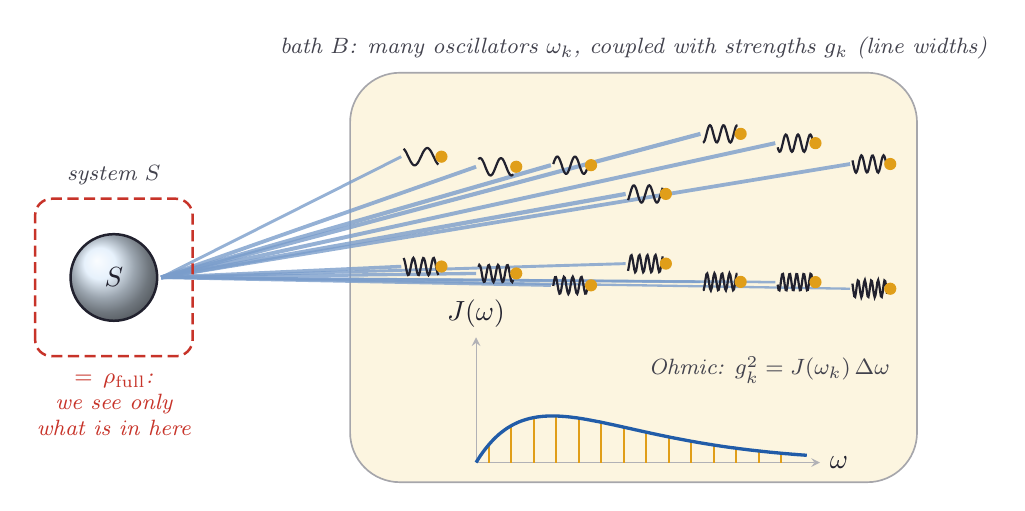
\begin{tikzpicture}[ink/.style={line width=0.9pt, ndInk}, faint/.style={line width=0.4pt, ndInk!35}, dashedink/.style={line width=0.5pt, ndInk!55, dash pattern=on 2.5pt off 2pt}, vec/.style={->, >=stealth, line width=1.2pt}, note/.style={font=\footnotesize\itshape, text=ndInk!85, align=center}, pointer/.style={->, >=stealth, line width=0.4pt, ndInk!60, shorten >=2pt, shorten <=1pt}, dot/.style={circle, fill=ndInk, inner sep=0pt, minimum size=3.4pt}, wash/.style={fill=ndSky, fill opacity=0.55}, every node/.style={text=ndInk}]
\definecolor{ndInk}{rgb}{0.13,0.13,0.18}
\definecolor{ndPaper}{rgb}{0.99,0.96,0.88}
\definecolor{ndSky}{rgb}{0.84,0.91,0.98}
\definecolor{ndRose}{rgb}{0.98,0.86,0.84}
\definecolor{ndBlue}{rgb}{0.13,0.36,0.66}
\definecolor{ndRed}{rgb}{0.78,0.20,0.16}
\definecolor{ndGold}{rgb}{0.88,0.62,0.10}
\definecolor{ndGreen}{rgb}{0.18,0.52,0.30}
\filldraw[fill=ndPaper, draw=ndInk!40, line width=0.6pt, rounded corners=18pt] (3.0,-2.6) rectangle (10.2,2.6);
\draw[line width=1.05pt, ndBlue!60, opacity=0.8] (0.600,0.000) -- (3.650,1.534);
\draw[line width=1.38pt, ndBlue!60, opacity=0.8] (0.600,0.000) -- (4.600,1.406);
\draw[line width=1.50pt, ndBlue!60, opacity=0.8] (0.600,0.000) -- (5.550,1.426);
\draw[line width=1.52pt, ndBlue!60, opacity=0.8] (0.600,0.000) -- (6.500,1.061);
\draw[line width=1.49pt, ndBlue!60, opacity=0.8] (0.600,0.000) -- (7.450,1.824);
\draw[line width=1.43pt, ndBlue!60, opacity=0.8] (0.600,0.000) -- (8.400,1.706);
\draw[line width=1.36pt, ndBlue!60, opacity=0.8] (0.600,0.000) -- (9.350,1.441);
\draw[line width=1.28pt, ndBlue!60, opacity=0.8] (0.600,0.000) -- (3.650,0.139);
\draw[line width=1.20pt, ndBlue!60, opacity=0.8] (0.600,0.000) -- (4.600,0.051);
\draw[line width=1.12pt, ndBlue!60, opacity=0.8] (0.600,0.000) -- (5.550,-0.100);
\draw[line width=1.05pt, ndBlue!60, opacity=0.8] (0.600,0.000) -- (6.500,0.176);
\draw[line width=0.97pt, ndBlue!60, opacity=0.8] (0.600,0.000) -- (7.450,-0.056);
\draw[line width=0.91pt, ndBlue!60, opacity=0.8] (0.600,0.000) -- (8.400,-0.059);
\draw[line width=0.84pt, ndBlue!60, opacity=0.8] (0.600,0.000) -- (9.350,-0.143);
\draw[line width=0.8pt, ndInk] (3.680,1.635) -- (3.691,1.622) -- (3.703,1.606) -- (3.714,1.586) -- (3.725,1.563) -- (3.736,1.540) -- (3.748,1.516) -- (3.759,1.492) -- (3.770,1.471) -- (3.782,1.453) -- (3.793,1.439) -- (3.804,1.429) -- (3.815,1.424) -- (3.827,1.425) -- (3.838,1.431) -- (3.849,1.442) -- (3.861,1.457) -- (3.872,1.476) -- (3.883,1.498) -- (3.894,1.522) -- (3.906,1.546) -- (3.917,1.570) -- (3.928,1.592) -- (3.939,1.611) -- (3.951,1.626) -- (3.962,1.637) -- (3.973,1.643) -- (3.985,1.644) -- (3.996,1.639) -- (4.007,1.629) -- (4.018,1.615) -- (4.030,1.597) -- (4.041,1.576) -- (4.052,1.553) -- (4.064,1.528) -- (4.075,1.505) -- (4.086,1.482) -- (4.097,1.462) -- (4.109,1.446) -- (4.120,1.434);
\fill[ndGold] (4.160,1.534) circle (2.2pt);
\draw[line width=0.8pt, ndInk] (4.630,1.502) -- (4.641,1.513) -- (4.653,1.516) -- (4.664,1.511) -- (4.675,1.499) -- (4.686,1.480) -- (4.698,1.456) -- (4.709,1.428) -- (4.720,1.399) -- (4.732,1.370) -- (4.743,1.344) -- (4.754,1.322) -- (4.765,1.306) -- (4.777,1.297) -- (4.788,1.296) -- (4.799,1.303) -- (4.811,1.317) -- (4.822,1.338) -- (4.833,1.363) -- (4.844,1.391) -- (4.856,1.421) -- (4.867,1.449) -- (4.878,1.474) -- (4.889,1.495) -- (4.901,1.509) -- (4.912,1.515) -- (4.923,1.514) -- (4.935,1.506) -- (4.946,1.490) -- (4.957,1.468) -- (4.968,1.442) -- (4.980,1.413) -- (4.991,1.384) -- (5.002,1.356) -- (5.014,1.332) -- (5.025,1.313) -- (5.036,1.301) -- (5.047,1.296) -- (5.059,1.299) -- (5.070,1.310);
\fill[ndGold] (5.110,1.406) circle (2.2pt);
\draw[line width=0.8pt, ndInk] (5.580,1.441) -- (5.591,1.474) -- (5.603,1.502) -- (5.614,1.523) -- (5.625,1.534) -- (5.636,1.535) -- (5.648,1.524) -- (5.659,1.504) -- (5.670,1.477) -- (5.682,1.444) -- (5.693,1.410) -- (5.704,1.377) -- (5.715,1.348) -- (5.727,1.328) -- (5.738,1.317) -- (5.749,1.317) -- (5.761,1.327) -- (5.772,1.348) -- (5.783,1.376) -- (5.794,1.408) -- (5.806,1.443) -- (5.817,1.476) -- (5.828,1.504) -- (5.839,1.524) -- (5.851,1.534) -- (5.862,1.534) -- (5.873,1.523) -- (5.885,1.503) -- (5.896,1.475) -- (5.907,1.442) -- (5.918,1.407) -- (5.930,1.375) -- (5.941,1.347) -- (5.952,1.327) -- (5.964,1.317) -- (5.975,1.317) -- (5.986,1.329) -- (5.997,1.349) -- (6.009,1.378) -- (6.020,1.411);
\fill[ndGold] (6.060,1.426) circle (2.2pt);
\draw[line width=0.8pt, ndInk] (6.530,0.982) -- (6.541,1.015) -- (6.553,1.053) -- (6.564,1.093) -- (6.575,1.128) -- (6.586,1.155) -- (6.598,1.169) -- (6.609,1.169) -- (6.620,1.155) -- (6.632,1.129) -- (6.643,1.093) -- (6.654,1.054) -- (6.665,1.016) -- (6.677,0.983) -- (6.688,0.960) -- (6.699,0.951) -- (6.711,0.955) -- (6.722,0.974) -- (6.733,1.004) -- (6.744,1.041) -- (6.756,1.080) -- (6.767,1.117) -- (6.778,1.147) -- (6.789,1.166) -- (6.801,1.170) -- (6.812,1.161) -- (6.823,1.138) -- (6.835,1.106) -- (6.846,1.067) -- (6.857,1.028) -- (6.868,0.993) -- (6.880,0.966) -- (6.891,0.952) -- (6.902,0.952) -- (6.914,0.967) -- (6.925,0.993) -- (6.936,1.028) -- (6.947,1.068) -- (6.959,1.106) -- (6.970,1.139);
\fill[ndGold] (7.010,1.061) circle (2.2pt);
\draw[line width=0.8pt, ndInk] (7.480,1.715) -- (7.491,1.718) -- (7.503,1.738) -- (7.514,1.773) -- (7.525,1.816) -- (7.536,1.860) -- (7.548,1.899) -- (7.559,1.925) -- (7.570,1.934) -- (7.582,1.925) -- (7.593,1.899) -- (7.604,1.861) -- (7.615,1.817) -- (7.627,1.774) -- (7.638,1.739) -- (7.649,1.718) -- (7.661,1.715) -- (7.672,1.730) -- (7.683,1.760) -- (7.694,1.802) -- (7.706,1.846) -- (7.717,1.887) -- (7.728,1.918) -- (7.739,1.933) -- (7.751,1.930) -- (7.762,1.909) -- (7.773,1.874) -- (7.785,1.831) -- (7.796,1.787) -- (7.807,1.749) -- (7.818,1.723) -- (7.830,1.714) -- (7.841,1.723) -- (7.852,1.749) -- (7.864,1.788) -- (7.875,1.832) -- (7.886,1.875) -- (7.897,1.910) -- (7.909,1.930) -- (7.920,1.933);
\fill[ndGold] (7.960,1.824) circle (2.2pt);
\draw[line width=0.8pt, ndInk] (8.430,1.653) -- (8.441,1.616) -- (8.453,1.597) -- (8.464,1.601) -- (8.475,1.626) -- (8.486,1.668) -- (8.498,1.717) -- (8.509,1.765) -- (8.520,1.800) -- (8.532,1.815) -- (8.543,1.809) -- (8.554,1.781) -- (8.565,1.738) -- (8.577,1.688) -- (8.588,1.642) -- (8.599,1.609) -- (8.611,1.596) -- (8.622,1.606) -- (8.633,1.636) -- (8.644,1.681) -- (8.656,1.731) -- (8.667,1.776) -- (8.678,1.806) -- (8.689,1.816) -- (8.701,1.803) -- (8.712,1.770) -- (8.723,1.724) -- (8.735,1.674) -- (8.746,1.631) -- (8.757,1.603) -- (8.768,1.596) -- (8.780,1.612) -- (8.791,1.647) -- (8.802,1.695) -- (8.814,1.744) -- (8.825,1.786) -- (8.836,1.811) -- (8.847,1.815) -- (8.859,1.796) -- (8.870,1.759);
\fill[ndGold] (8.910,1.706) circle (2.2pt);
\draw[line width=0.8pt, ndInk] (9.380,1.487) -- (9.391,1.433) -- (9.403,1.381) -- (9.414,1.344) -- (9.425,1.331) -- (9.436,1.346) -- (9.448,1.385) -- (9.459,1.438) -- (9.470,1.492) -- (9.482,1.533) -- (9.493,1.551) -- (9.504,1.542) -- (9.515,1.508) -- (9.527,1.457) -- (9.538,1.402) -- (9.549,1.357) -- (9.561,1.334) -- (9.572,1.337) -- (9.583,1.366) -- (9.594,1.414) -- (9.606,1.469) -- (9.617,1.517) -- (9.628,1.546) -- (9.639,1.549) -- (9.651,1.525) -- (9.662,1.480) -- (9.673,1.426) -- (9.685,1.375) -- (9.696,1.341) -- (9.707,1.332) -- (9.718,1.350) -- (9.730,1.391) -- (9.741,1.445) -- (9.752,1.498) -- (9.764,1.536) -- (9.775,1.551) -- (9.786,1.539) -- (9.797,1.502) -- (9.809,1.450) -- (9.820,1.396);
\fill[ndGold] (9.860,1.441) circle (2.2pt);
\draw[line width=0.8pt, ndInk] (3.680,0.247) -- (3.691,0.218) -- (3.703,0.166) -- (3.714,0.106) -- (3.725,0.056) -- (3.736,0.031) -- (3.748,0.038) -- (3.759,0.075) -- (3.770,0.131) -- (3.782,0.190) -- (3.793,0.234) -- (3.804,0.249) -- (3.815,0.232) -- (3.827,0.187) -- (3.838,0.128) -- (3.849,0.072) -- (3.861,0.036) -- (3.872,0.031) -- (3.883,0.058) -- (3.894,0.109) -- (3.906,0.169) -- (3.917,0.220) -- (3.928,0.247) -- (3.939,0.242) -- (3.951,0.206) -- (3.962,0.150) -- (3.973,0.091) -- (3.985,0.046) -- (3.996,0.029) -- (4.007,0.045) -- (4.018,0.089) -- (4.030,0.147) -- (4.041,0.204) -- (4.052,0.241) -- (4.064,0.248) -- (4.075,0.222) -- (4.086,0.172) -- (4.097,0.112) -- (4.109,0.060) -- (4.120,0.032);
\fill[ndGold] (4.160,0.139) circle (2.2pt);
\draw[line width=0.8pt, ndInk] (4.630,0.134) -- (4.641,0.160) -- (4.653,0.148) -- (4.664,0.101) -- (4.675,0.037) -- (4.686,-0.022) -- (4.698,-0.056) -- (4.709,-0.053) -- (4.720,-0.013) -- (4.732,0.049) -- (4.743,0.111) -- (4.754,0.152) -- (4.765,0.158) -- (4.777,0.126) -- (4.788,0.068) -- (4.799,0.004) -- (4.811,-0.044) -- (4.822,-0.059) -- (4.833,-0.036) -- (4.844,0.018) -- (4.856,0.083) -- (4.867,0.137) -- (4.878,0.160) -- (4.889,0.146) -- (4.901,0.098) -- (4.912,0.033) -- (4.923,-0.025) -- (4.935,-0.057) -- (4.946,-0.051) -- (4.957,-0.010) -- (4.968,0.053) -- (4.980,0.114) -- (4.991,0.154) -- (5.002,0.157) -- (5.014,0.123) -- (5.025,0.064) -- (5.036,-0.000) -- (5.047,-0.046) -- (5.059,-0.059) -- (5.070,-0.033);
\fill[ndGold] (5.110,0.051) circle (2.2pt);
\draw[line width=0.8pt, ndInk] (5.580,-0.107) -- (5.591,-0.039) -- (5.603,0.004) -- (5.614,0.005) -- (5.625,-0.036) -- (5.636,-0.103) -- (5.648,-0.169) -- (5.659,-0.206) -- (5.670,-0.201) -- (5.682,-0.154) -- (5.693,-0.085) -- (5.704,-0.023) -- (5.715,0.009) -- (5.727,-0.003) -- (5.738,-0.055) -- (5.749,-0.124) -- (5.761,-0.184) -- (5.772,-0.210) -- (5.783,-0.191) -- (5.794,-0.135) -- (5.806,-0.065) -- (5.817,-0.009) -- (5.828,0.010) -- (5.839,-0.015) -- (5.851,-0.075) -- (5.862,-0.145) -- (5.873,-0.196) -- (5.885,-0.209) -- (5.896,-0.177) -- (5.907,-0.114) -- (5.918,-0.045) -- (5.930,0.001) -- (5.941,0.007) -- (5.952,-0.030) -- (5.964,-0.096) -- (5.975,-0.163) -- (5.986,-0.205) -- (5.997,-0.203) -- (6.009,-0.160) -- (6.020,-0.093);
\fill[ndGold] (6.060,-0.100) circle (2.2pt);
\draw[line width=0.8pt, ndInk] (6.530,0.084) -- (6.541,0.144) -- (6.553,0.219) -- (6.564,0.274) -- (6.575,0.283) -- (6.586,0.243) -- (6.598,0.172) -- (6.609,0.102) -- (6.620,0.067) -- (6.632,0.082) -- (6.643,0.141) -- (6.654,0.216) -- (6.665,0.272) -- (6.677,0.284) -- (6.688,0.245) -- (6.699,0.175) -- (6.711,0.104) -- (6.722,0.067) -- (6.733,0.081) -- (6.744,0.138) -- (6.756,0.213) -- (6.767,0.271) -- (6.778,0.284) -- (6.789,0.248) -- (6.801,0.177) -- (6.812,0.107) -- (6.823,0.068) -- (6.835,0.080) -- (6.846,0.136) -- (6.857,0.211) -- (6.868,0.270) -- (6.880,0.285) -- (6.891,0.250) -- (6.902,0.180) -- (6.914,0.109) -- (6.925,0.069) -- (6.936,0.078) -- (6.947,0.133) -- (6.959,0.208) -- (6.970,0.268);
\fill[ndGold] (7.010,0.176) circle (2.2pt);
\draw[line width=0.8pt, ndInk] (7.480,-0.159) -- (7.491,-0.157) -- (7.503,-0.102) -- (7.514,-0.022) -- (7.525,0.040) -- (7.536,0.051) -- (7.548,0.006) -- (7.559,-0.071) -- (7.570,-0.141) -- (7.582,-0.166) -- (7.593,-0.133) -- (7.604,-0.059) -- (7.615,0.016) -- (7.627,0.053) -- (7.638,0.033) -- (7.649,-0.034) -- (7.661,-0.113) -- (7.672,-0.161) -- (7.683,-0.155) -- (7.694,-0.096) -- (7.706,-0.016) -- (7.717,0.043) -- (7.728,0.050) -- (7.739,0.001) -- (7.751,-0.078) -- (7.762,-0.145) -- (7.773,-0.165) -- (7.785,-0.128) -- (7.796,-0.053) -- (7.807,0.021) -- (7.818,0.054) -- (7.830,0.029) -- (7.841,-0.041) -- (7.852,-0.118) -- (7.864,-0.163) -- (7.875,-0.152) -- (7.886,-0.090) -- (7.897,-0.010) -- (7.909,0.046) -- (7.920,0.048);
\fill[ndGold] (7.960,-0.056) circle (2.2pt);
\draw[line width=0.8pt, ndInk] (8.430,-0.091) -- (8.441,-0.157) -- (8.453,-0.164) -- (8.464,-0.109) -- (8.475,-0.025) -- (8.486,0.039) -- (8.498,0.045) -- (8.509,-0.011) -- (8.520,-0.096) -- (8.532,-0.159) -- (8.543,-0.163) -- (8.554,-0.105) -- (8.565,-0.021) -- (8.577,0.041) -- (8.588,0.044) -- (8.599,-0.015) -- (8.611,-0.100) -- (8.622,-0.160) -- (8.633,-0.161) -- (8.644,-0.102) -- (8.656,-0.017) -- (8.667,0.043) -- (8.678,0.042) -- (8.689,-0.019) -- (8.701,-0.103) -- (8.712,-0.162) -- (8.723,-0.159) -- (8.735,-0.098) -- (8.746,-0.013) -- (8.757,0.044) -- (8.768,0.040) -- (8.780,-0.023) -- (8.791,-0.107) -- (8.802,-0.163) -- (8.814,-0.158) -- (8.825,-0.094) -- (8.836,-0.009) -- (8.847,0.046) -- (8.859,0.038) -- (8.870,-0.027);
\fill[ndGold] (8.910,-0.059) circle (2.2pt);
\draw[line width=0.8pt, ndInk] (9.380,-0.078) -- (9.391,-0.165) -- (9.403,-0.238) -- (9.414,-0.247) -- (9.425,-0.187) -- (9.436,-0.098) -- (9.448,-0.038) -- (9.459,-0.047) -- (9.470,-0.120) -- (9.482,-0.207) -- (9.493,-0.252) -- (9.504,-0.224) -- (9.515,-0.143) -- (9.527,-0.061) -- (9.538,-0.033) -- (9.549,-0.078) -- (9.561,-0.165) -- (9.572,-0.238) -- (9.583,-0.247) -- (9.594,-0.187) -- (9.606,-0.098) -- (9.617,-0.038) -- (9.628,-0.047) -- (9.639,-0.120) -- (9.651,-0.207) -- (9.662,-0.252) -- (9.673,-0.224) -- (9.685,-0.143) -- (9.696,-0.061) -- (9.707,-0.033) -- (9.718,-0.078) -- (9.730,-0.165) -- (9.741,-0.238) -- (9.752,-0.247) -- (9.764,-0.187) -- (9.775,-0.098) -- (9.786,-0.038) -- (9.797,-0.047) -- (9.809,-0.120) -- (9.820,-0.207);
\fill[ndGold] (9.860,-0.143) circle (2.2pt);
\shade[ball color=ndSky!80!white] (0.000,0.000) circle (0.55);
\draw[ink] (0.000,0.000) circle (0.55);
\node at (0.000,0.000) {$S$};
\draw[line width=0.9pt, ndRed, dash pattern=on 4pt off 2pt, rounded corners=6pt] (-1.0,-1.0) rectangle (1.0,1.0);
\node[note, anchor=north, text=ndRed] at (0,-1.1) {$\rhoS=\TrB\,\rho_{\rm full}$:\\ we see only\\ what is in here};
\node[note, anchor=south] at (6.6,2.65) {bath $B$: many oscillators $\omega_k$, coupled with strengths $g_k$ (line widths)};
\node[note, anchor=south] at (0,1.05) {system $S$};
\draw[faint, ->, >=stealth] (4.600,-2.350) -- (8.968,-2.350) node[right, text=ndInk] {$\omega$};
\draw[faint, ->, >=stealth] (4.600,-2.350) -- (4.600,-0.760) node[above, text=ndInk] {$J(\omega)$};
\draw[line width=0.8pt, ndGold] (4.762,-2.350) -- (4.762,-2.123);
\draw[line width=0.8pt, ndGold] (5.047,-2.350) -- (5.047,-1.882);
\draw[line width=0.8pt, ndGold] (5.333,-2.350) -- (5.333,-1.779);
\draw[line width=0.8pt, ndGold] (5.619,-2.350) -- (5.619,-1.760);
\draw[line width=0.8pt, ndGold] (5.905,-2.350) -- (5.905,-1.787);
\draw[line width=0.8pt, ndGold] (6.191,-2.350) -- (6.191,-1.839);
\draw[line width=0.8pt, ndGold] (6.476,-2.350) -- (6.476,-1.901);
\draw[line width=0.8pt, ndGold] (6.762,-2.350) -- (6.762,-1.965);
\draw[line width=0.8pt, ndGold] (7.048,-2.350) -- (7.048,-2.025);
\draw[line width=0.8pt, ndGold] (7.334,-2.350) -- (7.334,-2.080);
\draw[line width=0.8pt, ndGold] (7.620,-2.350) -- (7.620,-2.128);
\draw[line width=0.8pt, ndGold] (7.905,-2.350) -- (7.905,-2.169);
\draw[line width=0.8pt, ndGold] (8.191,-2.350) -- (8.191,-2.204);
\draw[line width=0.8pt, ndGold] (8.477,-2.350) -- (8.477,-2.232);
\draw[line width=1.2pt, ndBlue] (4.600,-2.350) -- (4.621,-2.316) -- (4.642,-2.283) -- (4.663,-2.252) -- (4.684,-2.222) -- (4.706,-2.193) -- (4.727,-2.166) -- (4.748,-2.140) -- (4.769,-2.115) -- (4.790,-2.091) -- (4.811,-2.069) -- (4.832,-2.047) -- (4.853,-2.027) -- (4.874,-2.007) -- (4.895,-1.989) -- (4.917,-1.971) -- (4.938,-1.955) -- (4.959,-1.939) -- (4.980,-1.924) -- (5.001,-1.910) -- (5.022,-1.897) -- (5.043,-1.885) -- (5.064,-1.873) -- (5.085,-1.862) -- (5.107,-1.852) -- (5.128,-1.842) -- (5.149,-1.833) -- (5.170,-1.825) -- (5.191,-1.817) -- (5.212,-1.810) -- (5.233,-1.804) -- (5.254,-1.798) -- (5.275,-1.792) -- (5.296,-1.787) -- (5.318,-1.783) -- (5.339,-1.778) -- (5.360,-1.775) -- (5.381,-1.771) -- (5.402,-1.769) -- (5.423,-1.766) -- (5.444,-1.764) -- (5.465,-1.762) -- (5.486,-1.761) -- (5.508,-1.760) -- (5.529,-1.759) -- (5.550,-1.759) -- (5.571,-1.759) -- (5.592,-1.759) -- (5.613,-1.759) -- (5.634,-1.760) -- (5.655,-1.761) -- (5.676,-1.762) -- (5.697,-1.764) -- (5.719,-1.765) -- (5.740,-1.767) -- (5.761,-1.769) -- (5.782,-1.771) -- (5.803,-1.773) -- (5.824,-1.776) -- (5.845,-1.779) -- (5.866,-1.781) -- (5.887,-1.784) -- (5.909,-1.788) -- (5.930,-1.791) -- (5.951,-1.794) -- (5.972,-1.798) -- (5.993,-1.801) -- (6.014,-1.805) -- (6.035,-1.809) -- (6.056,-1.813) -- (6.077,-1.817) -- (6.098,-1.821) -- (6.120,-1.825) -- (6.141,-1.829) -- (6.162,-1.833) -- (6.183,-1.837) -- (6.204,-1.842) -- (6.225,-1.846) -- (6.246,-1.851) -- (6.267,-1.855) -- (6.288,-1.860) -- (6.310,-1.864) -- (6.331,-1.869) -- (6.352,-1.873) -- (6.373,-1.878) -- (6.394,-1.883) -- (6.415,-1.887) -- (6.436,-1.892) -- (6.457,-1.897) -- (6.478,-1.902) -- (6.499,-1.906) -- (6.521,-1.911) -- (6.542,-1.916) -- (6.563,-1.920) -- (6.584,-1.925) -- (6.605,-1.930) -- (6.626,-1.935) -- (6.647,-1.939) -- (6.668,-1.944) -- (6.689,-1.949) -- (6.711,-1.953) -- (6.732,-1.958) -- (6.753,-1.963) -- (6.774,-1.967) -- (6.795,-1.972) -- (6.816,-1.977) -- (6.837,-1.981) -- (6.858,-1.986) -- (6.879,-1.990) -- (6.901,-1.995) -- (6.922,-1.999) -- (6.943,-2.004) -- (6.964,-2.008) -- (6.985,-2.012) -- (7.006,-2.017) -- (7.027,-2.021) -- (7.048,-2.025) -- (7.069,-2.030) -- (7.090,-2.034) -- (7.112,-2.038) -- (7.133,-2.042) -- (7.154,-2.046) -- (7.175,-2.050) -- (7.196,-2.054) -- (7.217,-2.058) -- (7.238,-2.062) -- (7.259,-2.066) -- (7.280,-2.070) -- (7.302,-2.074) -- (7.323,-2.078) -- (7.344,-2.082) -- (7.365,-2.085) -- (7.386,-2.089) -- (7.407,-2.093) -- (7.428,-2.097) -- (7.449,-2.100) -- (7.470,-2.104) -- (7.491,-2.107) -- (7.513,-2.111) -- (7.534,-2.114) -- (7.555,-2.118) -- (7.576,-2.121) -- (7.597,-2.124) -- (7.618,-2.128) -- (7.639,-2.131) -- (7.660,-2.134) -- (7.681,-2.137) -- (7.703,-2.141) -- (7.724,-2.144) -- (7.745,-2.147) -- (7.766,-2.150) -- (7.787,-2.153) -- (7.808,-2.156) -- (7.829,-2.159) -- (7.850,-2.162) -- (7.871,-2.164) -- (7.892,-2.167) -- (7.914,-2.170) -- (7.935,-2.173) -- (7.956,-2.176) -- (7.977,-2.178) -- (7.998,-2.181) -- (8.019,-2.183) -- (8.040,-2.186) -- (8.061,-2.189) -- (8.082,-2.191) -- (8.104,-2.194) -- (8.125,-2.196) -- (8.146,-2.198) -- (8.167,-2.201) -- (8.188,-2.203) -- (8.209,-2.205) -- (8.230,-2.208) -- (8.251,-2.210) -- (8.272,-2.212) -- (8.293,-2.214) -- (8.315,-2.217) -- (8.336,-2.219) -- (8.357,-2.221) -- (8.378,-2.223) -- (8.399,-2.225) -- (8.420,-2.227) -- (8.441,-2.229) -- (8.462,-2.231) -- (8.483,-2.233) -- (8.505,-2.235) -- (8.526,-2.237) -- (8.547,-2.238) -- (8.568,-2.240) -- (8.589,-2.242) -- (8.610,-2.244) -- (8.631,-2.246) -- (8.652,-2.247) -- (8.673,-2.249) -- (8.694,-2.251) -- (8.716,-2.252) -- (8.737,-2.254) -- (8.758,-2.255) -- (8.779,-2.257) -- (8.800,-2.259);
\node[note, anchor=west] at (6.668,-1.171) {Ohmic: $g_k^2=J(\omega_k)\,\Delta\omega$};
\end{tikzpicture}
}
\caption{A qubit $S$ coupled to a bath of oscillators, with line widths proportional to the couplings $g_k$ sampled from an Ohmic spectral density (inset). The partial trace keeps only what is inside the dashed window. Generated by \texttt{code/ch03\_bath.py}.}\label{fig:ch03:bath}
\end{figure}}
\ona{\endgraf\medskip\noindent\textit{Reading the figure.} The ball on the left is the system we care about, here a qubit. Each little spring on the right is one vibration mode of the environment: a photon mode of the electromagnetic field, a vibration of the crystal lattice, a resonance in the wiring of a chip. A thicker line means a stronger coupling between the qubit and that mode. The inset plots the spectral density $J(\omega)$: the horizontal axis is the frequency of a bath mode, the height says how strongly the qubit couples to modes of that frequency, and each stem is one of the springs drawn above.\endgraf\smallskip\noindent\textit{Why it matters.} The full system, a qubit together with a practically infinite number of bath modes, is far too large to simulate. What we can observe is only the qubit, the inside of the dashed window. For readers with a computer-science background, the partial trace $\TrB$ is the quantum analogue of \emph{marginalising} a joint probability distribution over the variables one does not observe; every master equation in this \chap{} is an attempt to describe the marginal without simulating the rest. For readers with a physics background: for a bath of harmonic oscillators coupled linearly to the system, the bath enters the second-order (Born) theory only through its correlation function, which is fixed by $J(\omega)$ and the temperature. Different hardware platforms differ to a large extent by their spectral densities.}
\onp{\begin{center}\resizebox{!}{0.6\textheight}{% Generated by code/needham.py -- do not edit by hand.
\definecolor{qocA}{rgb}{0.00,0.45,0.70}
\definecolor{qocB}{rgb}{0.90,0.60,0.00}
\definecolor{qocC}{rgb}{0.00,0.62,0.45}
\definecolor{qocD}{rgb}{0.80,0.40,0.00}
\definecolor{qocE}{rgb}{0.80,0.60,0.70}
\definecolor{qocF}{rgb}{0.35,0.70,0.90}
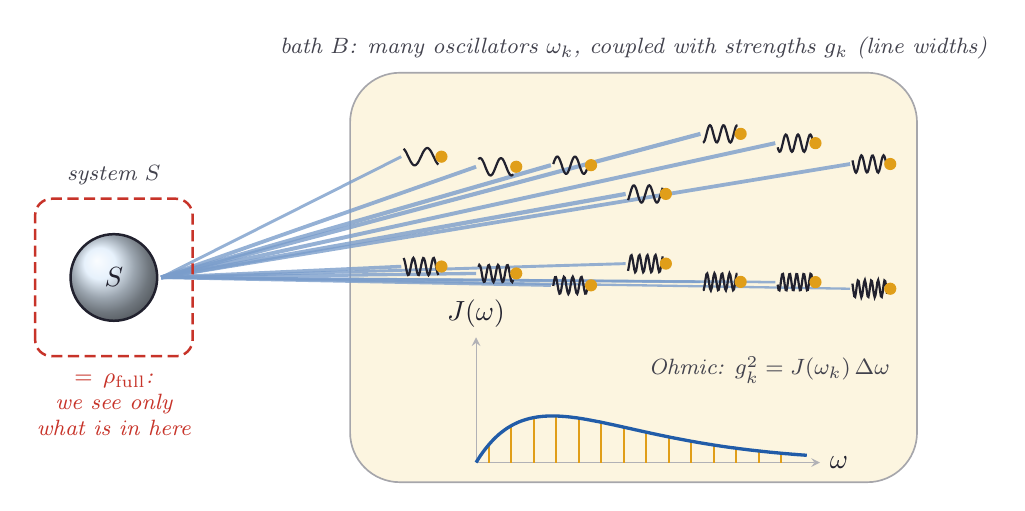
\begin{tikzpicture}[ink/.style={line width=0.9pt, ndInk}, faint/.style={line width=0.4pt, ndInk!35}, dashedink/.style={line width=0.5pt, ndInk!55, dash pattern=on 2.5pt off 2pt}, vec/.style={->, >=stealth, line width=1.2pt}, note/.style={font=\footnotesize\itshape, text=ndInk!85, align=center}, pointer/.style={->, >=stealth, line width=0.4pt, ndInk!60, shorten >=2pt, shorten <=1pt}, dot/.style={circle, fill=ndInk, inner sep=0pt, minimum size=3.4pt}, wash/.style={fill=ndSky, fill opacity=0.55}, every node/.style={text=ndInk}]
\definecolor{ndInk}{rgb}{0.13,0.13,0.18}
\definecolor{ndPaper}{rgb}{0.99,0.96,0.88}
\definecolor{ndSky}{rgb}{0.84,0.91,0.98}
\definecolor{ndRose}{rgb}{0.98,0.86,0.84}
\definecolor{ndBlue}{rgb}{0.13,0.36,0.66}
\definecolor{ndRed}{rgb}{0.78,0.20,0.16}
\definecolor{ndGold}{rgb}{0.88,0.62,0.10}
\definecolor{ndGreen}{rgb}{0.18,0.52,0.30}
\filldraw[fill=ndPaper, draw=ndInk!40, line width=0.6pt, rounded corners=18pt] (3.0,-2.6) rectangle (10.2,2.6);
\draw[line width=1.05pt, ndBlue!60, opacity=0.8] (0.600,0.000) -- (3.650,1.534);
\draw[line width=1.38pt, ndBlue!60, opacity=0.8] (0.600,0.000) -- (4.600,1.406);
\draw[line width=1.50pt, ndBlue!60, opacity=0.8] (0.600,0.000) -- (5.550,1.426);
\draw[line width=1.52pt, ndBlue!60, opacity=0.8] (0.600,0.000) -- (6.500,1.061);
\draw[line width=1.49pt, ndBlue!60, opacity=0.8] (0.600,0.000) -- (7.450,1.824);
\draw[line width=1.43pt, ndBlue!60, opacity=0.8] (0.600,0.000) -- (8.400,1.706);
\draw[line width=1.36pt, ndBlue!60, opacity=0.8] (0.600,0.000) -- (9.350,1.441);
\draw[line width=1.28pt, ndBlue!60, opacity=0.8] (0.600,0.000) -- (3.650,0.139);
\draw[line width=1.20pt, ndBlue!60, opacity=0.8] (0.600,0.000) -- (4.600,0.051);
\draw[line width=1.12pt, ndBlue!60, opacity=0.8] (0.600,0.000) -- (5.550,-0.100);
\draw[line width=1.05pt, ndBlue!60, opacity=0.8] (0.600,0.000) -- (6.500,0.176);
\draw[line width=0.97pt, ndBlue!60, opacity=0.8] (0.600,0.000) -- (7.450,-0.056);
\draw[line width=0.91pt, ndBlue!60, opacity=0.8] (0.600,0.000) -- (8.400,-0.059);
\draw[line width=0.84pt, ndBlue!60, opacity=0.8] (0.600,0.000) -- (9.350,-0.143);
\draw[line width=0.8pt, ndInk] (3.680,1.635) -- (3.691,1.622) -- (3.703,1.606) -- (3.714,1.586) -- (3.725,1.563) -- (3.736,1.540) -- (3.748,1.516) -- (3.759,1.492) -- (3.770,1.471) -- (3.782,1.453) -- (3.793,1.439) -- (3.804,1.429) -- (3.815,1.424) -- (3.827,1.425) -- (3.838,1.431) -- (3.849,1.442) -- (3.861,1.457) -- (3.872,1.476) -- (3.883,1.498) -- (3.894,1.522) -- (3.906,1.546) -- (3.917,1.570) -- (3.928,1.592) -- (3.939,1.611) -- (3.951,1.626) -- (3.962,1.637) -- (3.973,1.643) -- (3.985,1.644) -- (3.996,1.639) -- (4.007,1.629) -- (4.018,1.615) -- (4.030,1.597) -- (4.041,1.576) -- (4.052,1.553) -- (4.064,1.528) -- (4.075,1.505) -- (4.086,1.482) -- (4.097,1.462) -- (4.109,1.446) -- (4.120,1.434);
\fill[ndGold] (4.160,1.534) circle (2.2pt);
\draw[line width=0.8pt, ndInk] (4.630,1.502) -- (4.641,1.513) -- (4.653,1.516) -- (4.664,1.511) -- (4.675,1.499) -- (4.686,1.480) -- (4.698,1.456) -- (4.709,1.428) -- (4.720,1.399) -- (4.732,1.370) -- (4.743,1.344) -- (4.754,1.322) -- (4.765,1.306) -- (4.777,1.297) -- (4.788,1.296) -- (4.799,1.303) -- (4.811,1.317) -- (4.822,1.338) -- (4.833,1.363) -- (4.844,1.391) -- (4.856,1.421) -- (4.867,1.449) -- (4.878,1.474) -- (4.889,1.495) -- (4.901,1.509) -- (4.912,1.515) -- (4.923,1.514) -- (4.935,1.506) -- (4.946,1.490) -- (4.957,1.468) -- (4.968,1.442) -- (4.980,1.413) -- (4.991,1.384) -- (5.002,1.356) -- (5.014,1.332) -- (5.025,1.313) -- (5.036,1.301) -- (5.047,1.296) -- (5.059,1.299) -- (5.070,1.310);
\fill[ndGold] (5.110,1.406) circle (2.2pt);
\draw[line width=0.8pt, ndInk] (5.580,1.441) -- (5.591,1.474) -- (5.603,1.502) -- (5.614,1.523) -- (5.625,1.534) -- (5.636,1.535) -- (5.648,1.524) -- (5.659,1.504) -- (5.670,1.477) -- (5.682,1.444) -- (5.693,1.410) -- (5.704,1.377) -- (5.715,1.348) -- (5.727,1.328) -- (5.738,1.317) -- (5.749,1.317) -- (5.761,1.327) -- (5.772,1.348) -- (5.783,1.376) -- (5.794,1.408) -- (5.806,1.443) -- (5.817,1.476) -- (5.828,1.504) -- (5.839,1.524) -- (5.851,1.534) -- (5.862,1.534) -- (5.873,1.523) -- (5.885,1.503) -- (5.896,1.475) -- (5.907,1.442) -- (5.918,1.407) -- (5.930,1.375) -- (5.941,1.347) -- (5.952,1.327) -- (5.964,1.317) -- (5.975,1.317) -- (5.986,1.329) -- (5.997,1.349) -- (6.009,1.378) -- (6.020,1.411);
\fill[ndGold] (6.060,1.426) circle (2.2pt);
\draw[line width=0.8pt, ndInk] (6.530,0.982) -- (6.541,1.015) -- (6.553,1.053) -- (6.564,1.093) -- (6.575,1.128) -- (6.586,1.155) -- (6.598,1.169) -- (6.609,1.169) -- (6.620,1.155) -- (6.632,1.129) -- (6.643,1.093) -- (6.654,1.054) -- (6.665,1.016) -- (6.677,0.983) -- (6.688,0.960) -- (6.699,0.951) -- (6.711,0.955) -- (6.722,0.974) -- (6.733,1.004) -- (6.744,1.041) -- (6.756,1.080) -- (6.767,1.117) -- (6.778,1.147) -- (6.789,1.166) -- (6.801,1.170) -- (6.812,1.161) -- (6.823,1.138) -- (6.835,1.106) -- (6.846,1.067) -- (6.857,1.028) -- (6.868,0.993) -- (6.880,0.966) -- (6.891,0.952) -- (6.902,0.952) -- (6.914,0.967) -- (6.925,0.993) -- (6.936,1.028) -- (6.947,1.068) -- (6.959,1.106) -- (6.970,1.139);
\fill[ndGold] (7.010,1.061) circle (2.2pt);
\draw[line width=0.8pt, ndInk] (7.480,1.715) -- (7.491,1.718) -- (7.503,1.738) -- (7.514,1.773) -- (7.525,1.816) -- (7.536,1.860) -- (7.548,1.899) -- (7.559,1.925) -- (7.570,1.934) -- (7.582,1.925) -- (7.593,1.899) -- (7.604,1.861) -- (7.615,1.817) -- (7.627,1.774) -- (7.638,1.739) -- (7.649,1.718) -- (7.661,1.715) -- (7.672,1.730) -- (7.683,1.760) -- (7.694,1.802) -- (7.706,1.846) -- (7.717,1.887) -- (7.728,1.918) -- (7.739,1.933) -- (7.751,1.930) -- (7.762,1.909) -- (7.773,1.874) -- (7.785,1.831) -- (7.796,1.787) -- (7.807,1.749) -- (7.818,1.723) -- (7.830,1.714) -- (7.841,1.723) -- (7.852,1.749) -- (7.864,1.788) -- (7.875,1.832) -- (7.886,1.875) -- (7.897,1.910) -- (7.909,1.930) -- (7.920,1.933);
\fill[ndGold] (7.960,1.824) circle (2.2pt);
\draw[line width=0.8pt, ndInk] (8.430,1.653) -- (8.441,1.616) -- (8.453,1.597) -- (8.464,1.601) -- (8.475,1.626) -- (8.486,1.668) -- (8.498,1.717) -- (8.509,1.765) -- (8.520,1.800) -- (8.532,1.815) -- (8.543,1.809) -- (8.554,1.781) -- (8.565,1.738) -- (8.577,1.688) -- (8.588,1.642) -- (8.599,1.609) -- (8.611,1.596) -- (8.622,1.606) -- (8.633,1.636) -- (8.644,1.681) -- (8.656,1.731) -- (8.667,1.776) -- (8.678,1.806) -- (8.689,1.816) -- (8.701,1.803) -- (8.712,1.770) -- (8.723,1.724) -- (8.735,1.674) -- (8.746,1.631) -- (8.757,1.603) -- (8.768,1.596) -- (8.780,1.612) -- (8.791,1.647) -- (8.802,1.695) -- (8.814,1.744) -- (8.825,1.786) -- (8.836,1.811) -- (8.847,1.815) -- (8.859,1.796) -- (8.870,1.759);
\fill[ndGold] (8.910,1.706) circle (2.2pt);
\draw[line width=0.8pt, ndInk] (9.380,1.487) -- (9.391,1.433) -- (9.403,1.381) -- (9.414,1.344) -- (9.425,1.331) -- (9.436,1.346) -- (9.448,1.385) -- (9.459,1.438) -- (9.470,1.492) -- (9.482,1.533) -- (9.493,1.551) -- (9.504,1.542) -- (9.515,1.508) -- (9.527,1.457) -- (9.538,1.402) -- (9.549,1.357) -- (9.561,1.334) -- (9.572,1.337) -- (9.583,1.366) -- (9.594,1.414) -- (9.606,1.469) -- (9.617,1.517) -- (9.628,1.546) -- (9.639,1.549) -- (9.651,1.525) -- (9.662,1.480) -- (9.673,1.426) -- (9.685,1.375) -- (9.696,1.341) -- (9.707,1.332) -- (9.718,1.350) -- (9.730,1.391) -- (9.741,1.445) -- (9.752,1.498) -- (9.764,1.536) -- (9.775,1.551) -- (9.786,1.539) -- (9.797,1.502) -- (9.809,1.450) -- (9.820,1.396);
\fill[ndGold] (9.860,1.441) circle (2.2pt);
\draw[line width=0.8pt, ndInk] (3.680,0.247) -- (3.691,0.218) -- (3.703,0.166) -- (3.714,0.106) -- (3.725,0.056) -- (3.736,0.031) -- (3.748,0.038) -- (3.759,0.075) -- (3.770,0.131) -- (3.782,0.190) -- (3.793,0.234) -- (3.804,0.249) -- (3.815,0.232) -- (3.827,0.187) -- (3.838,0.128) -- (3.849,0.072) -- (3.861,0.036) -- (3.872,0.031) -- (3.883,0.058) -- (3.894,0.109) -- (3.906,0.169) -- (3.917,0.220) -- (3.928,0.247) -- (3.939,0.242) -- (3.951,0.206) -- (3.962,0.150) -- (3.973,0.091) -- (3.985,0.046) -- (3.996,0.029) -- (4.007,0.045) -- (4.018,0.089) -- (4.030,0.147) -- (4.041,0.204) -- (4.052,0.241) -- (4.064,0.248) -- (4.075,0.222) -- (4.086,0.172) -- (4.097,0.112) -- (4.109,0.060) -- (4.120,0.032);
\fill[ndGold] (4.160,0.139) circle (2.2pt);
\draw[line width=0.8pt, ndInk] (4.630,0.134) -- (4.641,0.160) -- (4.653,0.148) -- (4.664,0.101) -- (4.675,0.037) -- (4.686,-0.022) -- (4.698,-0.056) -- (4.709,-0.053) -- (4.720,-0.013) -- (4.732,0.049) -- (4.743,0.111) -- (4.754,0.152) -- (4.765,0.158) -- (4.777,0.126) -- (4.788,0.068) -- (4.799,0.004) -- (4.811,-0.044) -- (4.822,-0.059) -- (4.833,-0.036) -- (4.844,0.018) -- (4.856,0.083) -- (4.867,0.137) -- (4.878,0.160) -- (4.889,0.146) -- (4.901,0.098) -- (4.912,0.033) -- (4.923,-0.025) -- (4.935,-0.057) -- (4.946,-0.051) -- (4.957,-0.010) -- (4.968,0.053) -- (4.980,0.114) -- (4.991,0.154) -- (5.002,0.157) -- (5.014,0.123) -- (5.025,0.064) -- (5.036,-0.000) -- (5.047,-0.046) -- (5.059,-0.059) -- (5.070,-0.033);
\fill[ndGold] (5.110,0.051) circle (2.2pt);
\draw[line width=0.8pt, ndInk] (5.580,-0.107) -- (5.591,-0.039) -- (5.603,0.004) -- (5.614,0.005) -- (5.625,-0.036) -- (5.636,-0.103) -- (5.648,-0.169) -- (5.659,-0.206) -- (5.670,-0.201) -- (5.682,-0.154) -- (5.693,-0.085) -- (5.704,-0.023) -- (5.715,0.009) -- (5.727,-0.003) -- (5.738,-0.055) -- (5.749,-0.124) -- (5.761,-0.184) -- (5.772,-0.210) -- (5.783,-0.191) -- (5.794,-0.135) -- (5.806,-0.065) -- (5.817,-0.009) -- (5.828,0.010) -- (5.839,-0.015) -- (5.851,-0.075) -- (5.862,-0.145) -- (5.873,-0.196) -- (5.885,-0.209) -- (5.896,-0.177) -- (5.907,-0.114) -- (5.918,-0.045) -- (5.930,0.001) -- (5.941,0.007) -- (5.952,-0.030) -- (5.964,-0.096) -- (5.975,-0.163) -- (5.986,-0.205) -- (5.997,-0.203) -- (6.009,-0.160) -- (6.020,-0.093);
\fill[ndGold] (6.060,-0.100) circle (2.2pt);
\draw[line width=0.8pt, ndInk] (6.530,0.084) -- (6.541,0.144) -- (6.553,0.219) -- (6.564,0.274) -- (6.575,0.283) -- (6.586,0.243) -- (6.598,0.172) -- (6.609,0.102) -- (6.620,0.067) -- (6.632,0.082) -- (6.643,0.141) -- (6.654,0.216) -- (6.665,0.272) -- (6.677,0.284) -- (6.688,0.245) -- (6.699,0.175) -- (6.711,0.104) -- (6.722,0.067) -- (6.733,0.081) -- (6.744,0.138) -- (6.756,0.213) -- (6.767,0.271) -- (6.778,0.284) -- (6.789,0.248) -- (6.801,0.177) -- (6.812,0.107) -- (6.823,0.068) -- (6.835,0.080) -- (6.846,0.136) -- (6.857,0.211) -- (6.868,0.270) -- (6.880,0.285) -- (6.891,0.250) -- (6.902,0.180) -- (6.914,0.109) -- (6.925,0.069) -- (6.936,0.078) -- (6.947,0.133) -- (6.959,0.208) -- (6.970,0.268);
\fill[ndGold] (7.010,0.176) circle (2.2pt);
\draw[line width=0.8pt, ndInk] (7.480,-0.159) -- (7.491,-0.157) -- (7.503,-0.102) -- (7.514,-0.022) -- (7.525,0.040) -- (7.536,0.051) -- (7.548,0.006) -- (7.559,-0.071) -- (7.570,-0.141) -- (7.582,-0.166) -- (7.593,-0.133) -- (7.604,-0.059) -- (7.615,0.016) -- (7.627,0.053) -- (7.638,0.033) -- (7.649,-0.034) -- (7.661,-0.113) -- (7.672,-0.161) -- (7.683,-0.155) -- (7.694,-0.096) -- (7.706,-0.016) -- (7.717,0.043) -- (7.728,0.050) -- (7.739,0.001) -- (7.751,-0.078) -- (7.762,-0.145) -- (7.773,-0.165) -- (7.785,-0.128) -- (7.796,-0.053) -- (7.807,0.021) -- (7.818,0.054) -- (7.830,0.029) -- (7.841,-0.041) -- (7.852,-0.118) -- (7.864,-0.163) -- (7.875,-0.152) -- (7.886,-0.090) -- (7.897,-0.010) -- (7.909,0.046) -- (7.920,0.048);
\fill[ndGold] (7.960,-0.056) circle (2.2pt);
\draw[line width=0.8pt, ndInk] (8.430,-0.091) -- (8.441,-0.157) -- (8.453,-0.164) -- (8.464,-0.109) -- (8.475,-0.025) -- (8.486,0.039) -- (8.498,0.045) -- (8.509,-0.011) -- (8.520,-0.096) -- (8.532,-0.159) -- (8.543,-0.163) -- (8.554,-0.105) -- (8.565,-0.021) -- (8.577,0.041) -- (8.588,0.044) -- (8.599,-0.015) -- (8.611,-0.100) -- (8.622,-0.160) -- (8.633,-0.161) -- (8.644,-0.102) -- (8.656,-0.017) -- (8.667,0.043) -- (8.678,0.042) -- (8.689,-0.019) -- (8.701,-0.103) -- (8.712,-0.162) -- (8.723,-0.159) -- (8.735,-0.098) -- (8.746,-0.013) -- (8.757,0.044) -- (8.768,0.040) -- (8.780,-0.023) -- (8.791,-0.107) -- (8.802,-0.163) -- (8.814,-0.158) -- (8.825,-0.094) -- (8.836,-0.009) -- (8.847,0.046) -- (8.859,0.038) -- (8.870,-0.027);
\fill[ndGold] (8.910,-0.059) circle (2.2pt);
\draw[line width=0.8pt, ndInk] (9.380,-0.078) -- (9.391,-0.165) -- (9.403,-0.238) -- (9.414,-0.247) -- (9.425,-0.187) -- (9.436,-0.098) -- (9.448,-0.038) -- (9.459,-0.047) -- (9.470,-0.120) -- (9.482,-0.207) -- (9.493,-0.252) -- (9.504,-0.224) -- (9.515,-0.143) -- (9.527,-0.061) -- (9.538,-0.033) -- (9.549,-0.078) -- (9.561,-0.165) -- (9.572,-0.238) -- (9.583,-0.247) -- (9.594,-0.187) -- (9.606,-0.098) -- (9.617,-0.038) -- (9.628,-0.047) -- (9.639,-0.120) -- (9.651,-0.207) -- (9.662,-0.252) -- (9.673,-0.224) -- (9.685,-0.143) -- (9.696,-0.061) -- (9.707,-0.033) -- (9.718,-0.078) -- (9.730,-0.165) -- (9.741,-0.238) -- (9.752,-0.247) -- (9.764,-0.187) -- (9.775,-0.098) -- (9.786,-0.038) -- (9.797,-0.047) -- (9.809,-0.120) -- (9.820,-0.207);
\fill[ndGold] (9.860,-0.143) circle (2.2pt);
\shade[ball color=ndSky!80!white] (0.000,0.000) circle (0.55);
\draw[ink] (0.000,0.000) circle (0.55);
\node at (0.000,0.000) {$S$};
\draw[line width=0.9pt, ndRed, dash pattern=on 4pt off 2pt, rounded corners=6pt] (-1.0,-1.0) rectangle (1.0,1.0);
\node[note, anchor=north, text=ndRed] at (0,-1.1) {$\rhoS=\TrB\,\rho_{\rm full}$:\\ we see only\\ what is in here};
\node[note, anchor=south] at (6.6,2.65) {bath $B$: many oscillators $\omega_k$, coupled with strengths $g_k$ (line widths)};
\node[note, anchor=south] at (0,1.05) {system $S$};
\draw[faint, ->, >=stealth] (4.600,-2.350) -- (8.968,-2.350) node[right, text=ndInk] {$\omega$};
\draw[faint, ->, >=stealth] (4.600,-2.350) -- (4.600,-0.760) node[above, text=ndInk] {$J(\omega)$};
\draw[line width=0.8pt, ndGold] (4.762,-2.350) -- (4.762,-2.123);
\draw[line width=0.8pt, ndGold] (5.047,-2.350) -- (5.047,-1.882);
\draw[line width=0.8pt, ndGold] (5.333,-2.350) -- (5.333,-1.779);
\draw[line width=0.8pt, ndGold] (5.619,-2.350) -- (5.619,-1.760);
\draw[line width=0.8pt, ndGold] (5.905,-2.350) -- (5.905,-1.787);
\draw[line width=0.8pt, ndGold] (6.191,-2.350) -- (6.191,-1.839);
\draw[line width=0.8pt, ndGold] (6.476,-2.350) -- (6.476,-1.901);
\draw[line width=0.8pt, ndGold] (6.762,-2.350) -- (6.762,-1.965);
\draw[line width=0.8pt, ndGold] (7.048,-2.350) -- (7.048,-2.025);
\draw[line width=0.8pt, ndGold] (7.334,-2.350) -- (7.334,-2.080);
\draw[line width=0.8pt, ndGold] (7.620,-2.350) -- (7.620,-2.128);
\draw[line width=0.8pt, ndGold] (7.905,-2.350) -- (7.905,-2.169);
\draw[line width=0.8pt, ndGold] (8.191,-2.350) -- (8.191,-2.204);
\draw[line width=0.8pt, ndGold] (8.477,-2.350) -- (8.477,-2.232);
\draw[line width=1.2pt, ndBlue] (4.600,-2.350) -- (4.621,-2.316) -- (4.642,-2.283) -- (4.663,-2.252) -- (4.684,-2.222) -- (4.706,-2.193) -- (4.727,-2.166) -- (4.748,-2.140) -- (4.769,-2.115) -- (4.790,-2.091) -- (4.811,-2.069) -- (4.832,-2.047) -- (4.853,-2.027) -- (4.874,-2.007) -- (4.895,-1.989) -- (4.917,-1.971) -- (4.938,-1.955) -- (4.959,-1.939) -- (4.980,-1.924) -- (5.001,-1.910) -- (5.022,-1.897) -- (5.043,-1.885) -- (5.064,-1.873) -- (5.085,-1.862) -- (5.107,-1.852) -- (5.128,-1.842) -- (5.149,-1.833) -- (5.170,-1.825) -- (5.191,-1.817) -- (5.212,-1.810) -- (5.233,-1.804) -- (5.254,-1.798) -- (5.275,-1.792) -- (5.296,-1.787) -- (5.318,-1.783) -- (5.339,-1.778) -- (5.360,-1.775) -- (5.381,-1.771) -- (5.402,-1.769) -- (5.423,-1.766) -- (5.444,-1.764) -- (5.465,-1.762) -- (5.486,-1.761) -- (5.508,-1.760) -- (5.529,-1.759) -- (5.550,-1.759) -- (5.571,-1.759) -- (5.592,-1.759) -- (5.613,-1.759) -- (5.634,-1.760) -- (5.655,-1.761) -- (5.676,-1.762) -- (5.697,-1.764) -- (5.719,-1.765) -- (5.740,-1.767) -- (5.761,-1.769) -- (5.782,-1.771) -- (5.803,-1.773) -- (5.824,-1.776) -- (5.845,-1.779) -- (5.866,-1.781) -- (5.887,-1.784) -- (5.909,-1.788) -- (5.930,-1.791) -- (5.951,-1.794) -- (5.972,-1.798) -- (5.993,-1.801) -- (6.014,-1.805) -- (6.035,-1.809) -- (6.056,-1.813) -- (6.077,-1.817) -- (6.098,-1.821) -- (6.120,-1.825) -- (6.141,-1.829) -- (6.162,-1.833) -- (6.183,-1.837) -- (6.204,-1.842) -- (6.225,-1.846) -- (6.246,-1.851) -- (6.267,-1.855) -- (6.288,-1.860) -- (6.310,-1.864) -- (6.331,-1.869) -- (6.352,-1.873) -- (6.373,-1.878) -- (6.394,-1.883) -- (6.415,-1.887) -- (6.436,-1.892) -- (6.457,-1.897) -- (6.478,-1.902) -- (6.499,-1.906) -- (6.521,-1.911) -- (6.542,-1.916) -- (6.563,-1.920) -- (6.584,-1.925) -- (6.605,-1.930) -- (6.626,-1.935) -- (6.647,-1.939) -- (6.668,-1.944) -- (6.689,-1.949) -- (6.711,-1.953) -- (6.732,-1.958) -- (6.753,-1.963) -- (6.774,-1.967) -- (6.795,-1.972) -- (6.816,-1.977) -- (6.837,-1.981) -- (6.858,-1.986) -- (6.879,-1.990) -- (6.901,-1.995) -- (6.922,-1.999) -- (6.943,-2.004) -- (6.964,-2.008) -- (6.985,-2.012) -- (7.006,-2.017) -- (7.027,-2.021) -- (7.048,-2.025) -- (7.069,-2.030) -- (7.090,-2.034) -- (7.112,-2.038) -- (7.133,-2.042) -- (7.154,-2.046) -- (7.175,-2.050) -- (7.196,-2.054) -- (7.217,-2.058) -- (7.238,-2.062) -- (7.259,-2.066) -- (7.280,-2.070) -- (7.302,-2.074) -- (7.323,-2.078) -- (7.344,-2.082) -- (7.365,-2.085) -- (7.386,-2.089) -- (7.407,-2.093) -- (7.428,-2.097) -- (7.449,-2.100) -- (7.470,-2.104) -- (7.491,-2.107) -- (7.513,-2.111) -- (7.534,-2.114) -- (7.555,-2.118) -- (7.576,-2.121) -- (7.597,-2.124) -- (7.618,-2.128) -- (7.639,-2.131) -- (7.660,-2.134) -- (7.681,-2.137) -- (7.703,-2.141) -- (7.724,-2.144) -- (7.745,-2.147) -- (7.766,-2.150) -- (7.787,-2.153) -- (7.808,-2.156) -- (7.829,-2.159) -- (7.850,-2.162) -- (7.871,-2.164) -- (7.892,-2.167) -- (7.914,-2.170) -- (7.935,-2.173) -- (7.956,-2.176) -- (7.977,-2.178) -- (7.998,-2.181) -- (8.019,-2.183) -- (8.040,-2.186) -- (8.061,-2.189) -- (8.082,-2.191) -- (8.104,-2.194) -- (8.125,-2.196) -- (8.146,-2.198) -- (8.167,-2.201) -- (8.188,-2.203) -- (8.209,-2.205) -- (8.230,-2.208) -- (8.251,-2.210) -- (8.272,-2.212) -- (8.293,-2.214) -- (8.315,-2.217) -- (8.336,-2.219) -- (8.357,-2.221) -- (8.378,-2.223) -- (8.399,-2.225) -- (8.420,-2.227) -- (8.441,-2.229) -- (8.462,-2.231) -- (8.483,-2.233) -- (8.505,-2.235) -- (8.526,-2.237) -- (8.547,-2.238) -- (8.568,-2.240) -- (8.589,-2.242) -- (8.610,-2.244) -- (8.631,-2.246) -- (8.652,-2.247) -- (8.673,-2.249) -- (8.694,-2.251) -- (8.716,-2.252) -- (8.737,-2.254) -- (8.758,-2.255) -- (8.779,-2.257) -- (8.800,-2.259);
\node[note, anchor=west] at (6.668,-1.171) {Ohmic: $g_k^2=J(\omega_k)\,\Delta\omega$};
\end{tikzpicture}
}\end{center}}
\end{frame}

\begin{frame}\ft{Two kinds of description}
\ona{On a theoretical level, any valid description should correspond (at least approximately) to the evolution governed by tracing out the environment from the dynamics determined by the full Hamiltonian \eqref{eq:ch03:hamil_full}. The temporal evolution of $S$ can be formally characterised either by utilising \emph{quantum master equations} or by employing \emph{dynamical maps}. Master equations are ordinary differential equations in which the state of the reduced subsystem serves as the unknown variable,}
\begin{equation}\label{eq:ch03:first_master}
\dot{\rhoS}\left(t\right) = F\left(\rhoS\right),
\end{equation}
\ona{where $F$ represents a superoperator that maps the reduced state (in general, its whole history $\rhoS(\cdot)$) to its time derivative. Relationships of this type are typically numerically solvable when supplied with a suitable initial condition \cite{Breuer_Petruccione_2010a}. Dynamical maps, on the other hand, are a closed-form alternative: a map $\mathcal{E}_{t_{1},t_{2}}$ governs the evolution from $t_1$ to $t_2$ if $\mathcal{E}_{t_{1},t_{2}}(\rhoS(t_{1}))=\rhoS(t_{2})$. The maps are required to be completely positive, trace preserving and Hermiticity preserving; their structure and the notion of Markovianity are the subject of \Chap~\ref{C.GeometryChannels}. Here we concentrate on master equations, since these are what we recast as dynamical systems.}
\onp{\begin{itemize}\setlength\itemsep{0.6em}
\item \textbf{Master equations}: ODEs $\dot\rhoS(t)=F(\rhoS)$, $F$ a superoperator, possibly depending on the history. Infinitesimal description. \alert{This \chap{}.}
\item \textbf{Dynamical maps}: $\mathcal E_{t_1,t_2}(\rhoS(t_1))=\rhoS(t_2)$, completely positive and trace preserving. Finite-time description. \Chap~\ref{C.GeometryChannels}.
\item Master equations come in two families: \emph{phenomenological} (GKSL) and \emph{perturbative} (Nakajima--Zwanzig, Redfield, \dots).
\end{itemize}}
\end{frame}

\section{The GKSL master equation}

\begin{frame}\ft{From a Kraus decomposition to a master equation}
\ona{Let us start with perhaps the most famous of quantum master equations, namely the Lindblad or GKSL (after Gorini, Kossakowski, Sudarshan and Lindblad) equation. We follow \cite{Hall2014}, and in part \cite{gorini1976completely}, and derive its canonical form, which can be Markovian or non-Markovian. Any evolution of the reduced state that starts from a product state admits a Kraus decomposition (\Chap~\ref{C.GeometryChannels})}
\onp{Start from a Kraus decomposition}
\begin{equation}\label{eq:ch03:kraus}
\rhoS(t)=\sum_jE_j(t)\rhoS(0)E_j^\dagger(t).
\end{equation}
\ona{Taking a time derivative,}
\onp{and differentiate:}
\begin{equation}
    \dot\rhoS(t)=\sum_j \left(\dot E_j(t)\rhoS(0)E_j^\dagger(t)+E_j(t)\rhoS(0)\dot E_j^\dagger(t)\right).
\end{equation}
\ona{Here we have assumed that the Kraus operators themselves are differentiable, which is justified when the system--environment Hamiltonian is smooth. If the dynamical map is invertible, we can re-express $\rhoS(0)=\sum_j P_j(t)\rhoS(t)Q_j^\dagger(t)$ for some system operators $P_j$, $Q_j$, and hence $\dot \rhoS=\sum_m A_m(t)\rhoS B_m^\dagger(t)$ for suitable operators $A_m,B_m$. Expanding $A_m$ and $B_m$ in the orthonormal basis \eqref{eq:ch02:basis_conditions}, $A_m=\sum_nF_na_{nm}$, $B_m=\sum_nF_nb_{nm}$, gives the unique decomposition}
\onp{Invert the map, $\rhoS(0)=\sum_jP_j\rhoS(t)Q_j^\dagger$, and expand everything in the basis $\{F_m\}$ of \eqref{eq:ch02:basis_conditions}:}
\begin{equation}\label{eq:ch03:cmn}
    \dot\rhoS(t)=\sum_{m,n=0}^{N^2-1} c_{mn}F_m\rhoS(t) F_n,\qquad c_{mn}\coloneqq \sum_{p} a_{mp}\bar b_{np},
\end{equation}
\ona{where the matrix $(c_{mn})$ is Hermitian. Splitting off the terms with $m=0$ or $n=0$ (those containing the identity) and using that $\dot\rhoS$ is traceless yields the canonical form on the next slide.}
\onp{$(c_{mn})$ Hermitian. Split off $m=0$ or $n=0$ and use $\Tr\dot\rhoS=0$.}
\end{frame}

\begin{frame}\ft{The canonical GKSL equation}
\begin{thm}[Canonical GKSL form \cite{Hall2014,gorini1976completely}]\label{thm:ch03:gksl}
Under the assumptions above, the reduced state obeys
\begin{equation}\label{eq:ch03:gksl}
        \dot \rhoS(t)= -\imath \comm{H(t)}{\rhoS(t)}+
        \sum_{j,k=1}^{N^2-1}\gamma_{jk}(t)\Big(F_j\rhoS(t) F_k-\tfrac{1}{2}\acomm{F_kF_j}{\rhoS(t)}\Big),
\end{equation}
where $H(t)$ is Hermitian and $\gamma(t)=(\gamma_{jk}(t))$ is a Hermitian $(N^2-1)\times(N^2-1)$ matrix, the \emph{Kossakowski} (or decoherence) matrix.
\end{thm}
\ona{Explicitly, with $C\coloneqq \frac12 \frac{c_{00}}{N}+\sum_{j\ge1}\frac{c_{j0}}{\sqrt{N}}F_j$ one has
\[H(t)= \tfrac{\imath}{2}\big(C(t)-C^\dagger(t)\big),\qquad \gamma_{jk}(t)=\sum_{l}\Tr[F_jA_l(t)]\,\Tr[F_kB_l^\dagger(t)].\]
If $\gamma$ is positive semidefinite and time independent, we get the ordinary Markovian form of the GKSL equation \cite{Lindblad1976,gorini1976completely}. By diagonalising $\gamma=U\tilde\gamma U^\dagger$ and defining $L_k(t)\coloneqq \sum_{j}U_{jk}(t)F_j$ we find the well-known \emph{Lindblad form}}
\onp{$H=\tfrac\imath2(C-C^\dagger)$ and $\gamma_{jk}=\sum_l\Tr[F_jA_l]\Tr[F_kB_l^\dagger]$ are explicit. $\gamma\succeq0$ constant $\Rightarrow$ Markovian GKSL \cite{Lindblad1976,gorini1976completely}.}
\end{frame}

\begin{frame}\ft{The Lindblad form}
\onp{Diagonalise $\gamma=U\tilde\gamma U^\dagger$ and set $L_k=\sum_jU_{jk}F_j$: \alert{Lindblad form}}
\begin{equation}\label{eq:ch03:lindblad}
        \dot\rhoS(t) = -\imath\comm{H(t)}{\rhoS(t)}
        +\sum_{j=1}^{N^2-1}\tilde\gamma_j(t)\Big(L_j(t)\rhoS(t) L_j^\dagger(t) -\tfrac12\acomm{L_j^\dagger(t)L_j(t)}{\rhoS(t)}\Big),
\end{equation}
\ona{with \emph{jump operators} $L_j$ and rates $\tilde\gamma_j$. In the time-independent case the solution is a semigroup, $\rhoS(t)=\Phi(t)\rhoS(0)$ with $\Phi(t)=\exp(\Lind t)$, and Gorini, Kossakowski and Sudarshan showed that every generator of a completely positive trace-preserving semigroup has the form \eqref{eq:ch03:gksl} with constant $\gamma\succeq0$; see also \cite{Breuer2016}. Negative eigenvalues of $\gamma(t)$ signal non-Markovianity (\Chap~\ref{C.GeometryChannels}).}
\onp{Jump operators $L_j$, rates $\tilde\gamma_j$. Negative $\tilde\gamma_j(t)$ $\Leftrightarrow$ non-Markovian (\Chap~\ref{C.GeometryChannels}). Constant, non-negative rates: the \alert{Markovian} Lindblad equation}
\ona{In the Markovian case, with time-independent jump operators and rates $\tilde\gamma_j\ge0$, the equation reads}
\begin{equation}\label{eq:ch03:lindblad-markov}
\dot\rhoS=\Lind\rhoS\coloneqq-\imath\comm{H}{\rhoS}+\sum_j\tilde\gamma_j\Big(L_j\rhoS L_j^\dagger-\tfrac12\acomm{L_j^\dagger L_j}{\rhoS}\Big),\qquad \rhoS(t)=\ee^{\Lind t}\rhoS(0).
\end{equation}
\end{frame}

\begin{frame}\ft{Markovian and non-Markovian evolution}
\ona{What distinguishes Markovian from non-Markovian dynamics can be seen in an exactly solvable model: a qubit coupled resonantly to a bath with the Lorentzian spectral density $J(\omega)=\frac{\gamma_0\lambda^2}{2\pi((\omega_0-\omega)^2+\lambda^2)}$ \cite{Breuer_Petruccione_2010a}. The excited-state amplitude is multiplied by a function $G(t)$, and the reduced dynamics obey the master equation $\dot\rhoS=\gamma(t)\big(\sigma_-\rhoS\sigma_+-\tfrac12\acomm{\sigma_+\sigma_-}{\rhoS}\big)$ with the time-dependent rate $\gamma(t)=-2\,\tfrac{\mathrm d}{\mathrm dt}\log\abs{G(t)}$. A good measure of the state of the dynamics is \emph{distinguishability}: the trace distance between the evolved states of $\ket+$ and $\ket-$, which here equals $\abs{G(t)}$. Under any Markovian evolution, distinguishability can only decrease, since information flows from the system into the bath and never returns. For weak coupling ($\lambda\gg\gamma_0$) this is what happens, and $\gamma(t)\approx\gamma_0>0$ (Figure~\ref{fig:ch03:nonmarkov}). For strong coupling ($\lambda<2\gamma_0$) the distinguishability \emph{revives}: information flows back from the bath. Precisely on the revivals the rate $\gamma(t)$ is negative, which is the signature of non-Markovianity mentioned above.}
\onp{Exactly solvable: qubit, Lorentzian bath. Distinguishability of $\ket\pm$ $=\abs{G(t)}$; rate $\gamma(t)=-2\frac{\mathrm d}{\mathrm dt}\log\abs{G}$.}
\ona{\begin{figure}[H]\centering
\resizebox{\linewidth}{!}{% Generated by code/needham.py -- do not edit by hand.
\definecolor{qocA}{rgb}{0.00,0.45,0.70}
\definecolor{qocB}{rgb}{0.90,0.60,0.00}
\definecolor{qocC}{rgb}{0.00,0.62,0.45}
\definecolor{qocD}{rgb}{0.80,0.40,0.00}
\definecolor{qocE}{rgb}{0.80,0.60,0.70}
\definecolor{qocF}{rgb}{0.35,0.70,0.90}
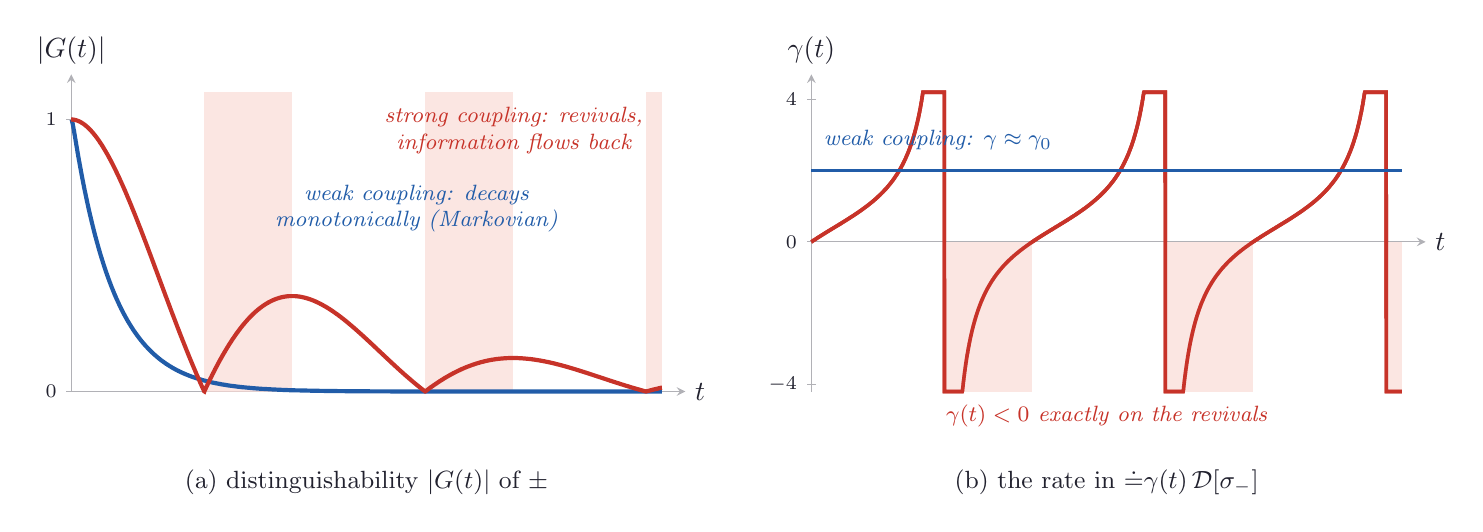
\begin{tikzpicture}[ink/.style={line width=0.9pt, ndInk}, faint/.style={line width=0.4pt, ndInk!35}, dashedink/.style={line width=0.5pt, ndInk!55, dash pattern=on 2.5pt off 2pt}, vec/.style={->, >=stealth, line width=1.2pt}, note/.style={font=\footnotesize\itshape, text=ndInk!85, align=center}, pointer/.style={->, >=stealth, line width=0.4pt, ndInk!60, shorten >=2pt, shorten <=1pt}, dot/.style={circle, fill=ndInk, inner sep=0pt, minimum size=3.4pt}, wash/.style={fill=ndSky, fill opacity=0.55}, every node/.style={text=ndInk}]
\definecolor{ndInk}{rgb}{0.13,0.13,0.18}
\definecolor{ndPaper}{rgb}{0.99,0.96,0.88}
\definecolor{ndSky}{rgb}{0.84,0.91,0.98}
\definecolor{ndRose}{rgb}{0.98,0.86,0.84}
\definecolor{ndBlue}{rgb}{0.13,0.36,0.66}
\definecolor{ndRed}{rgb}{0.78,0.20,0.16}
\definecolor{ndGold}{rgb}{0.88,0.62,0.10}
\definecolor{ndGreen}{rgb}{0.18,0.52,0.30}
\draw[faint, ->, >=stealth] (0.000,0.000) -- (7.800,0.000) node[right, text=ndInk] {$t$};
\draw[faint, ->, >=stealth] (0.000,0.000) -- (0.000,4.028) node[above, text=ndInk] {$|G(t)|$};
\draw[faint] (0.060,0.000) -- (-0.060,0.000) node[left, font=\scriptsize, text=ndInk] {$0$};
\draw[faint] (0.060,3.455) -- (-0.060,3.455) node[left, font=\scriptsize, text=ndInk] {$1$};
\fill[ndRose, fill opacity=0.7] (1.691,0.000) rectangle (2.803,3.800);
\fill[ndRose, fill opacity=0.7] (4.494,0.000) rectangle (5.608,3.800);
\fill[ndRose, fill opacity=0.7] (7.299,0.000) rectangle (7.497,3.800);
\draw[line width=1.5pt, ndBlue] (0.000,3.455) -- (0.003,3.453) -- (0.005,3.448) -- (0.008,3.442) -- (0.011,3.433) -- (0.013,3.423) -- (0.016,3.411) -- (0.019,3.399) -- (0.021,3.386) -- (0.024,3.372) -- (0.027,3.357) -- (0.029,3.342) -- (0.032,3.327) -- (0.035,3.312) -- (0.038,3.296) -- (0.040,3.280) -- (0.043,3.264) -- (0.046,3.248) -- (0.048,3.232) -- (0.051,3.216) -- (0.054,3.200) -- (0.056,3.184) -- (0.059,3.168) -- (0.062,3.152) -- (0.064,3.136) -- (0.067,3.120) -- (0.070,3.104) -- (0.072,3.088) -- (0.075,3.073) -- (0.078,3.057) -- (0.080,3.041) -- (0.083,3.026) -- (0.086,3.010) -- (0.088,2.995) -- (0.091,2.980) -- (0.094,2.964) -- (0.096,2.949) -- (0.099,2.934) -- (0.102,2.919) -- (0.105,2.904) -- (0.107,2.889) -- (0.110,2.875) -- (0.113,2.860) -- (0.115,2.845) -- (0.118,2.831) -- (0.121,2.816) -- (0.123,2.802) -- (0.126,2.787) -- (0.129,2.773) -- (0.131,2.759) -- (0.134,2.745) -- (0.137,2.731) -- (0.139,2.717) -- (0.142,2.703) -- (0.145,2.689) -- (0.147,2.675) -- (0.150,2.662) -- (0.153,2.648) -- (0.155,2.634) -- (0.158,2.621) -- (0.161,2.607) -- (0.163,2.594) -- (0.166,2.581) -- (0.169,2.568) -- (0.171,2.554) -- (0.174,2.541) -- (0.177,2.528) -- (0.180,2.515) -- (0.182,2.503) -- (0.185,2.490) -- (0.188,2.477) -- (0.190,2.464) -- (0.193,2.452) -- (0.196,2.439) -- (0.198,2.427) -- (0.201,2.414) -- (0.204,2.402) -- (0.206,2.390) -- (0.209,2.377) -- (0.212,2.365) -- (0.214,2.353) -- (0.217,2.341) -- (0.220,2.329) -- (0.222,2.317) -- (0.225,2.305) -- (0.228,2.293) -- (0.230,2.282) -- (0.233,2.270) -- (0.236,2.258) -- (0.238,2.247) -- (0.241,2.235) -- (0.244,2.224) -- (0.247,2.212) -- (0.249,2.201) -- (0.252,2.190) -- (0.255,2.179) -- (0.257,2.167) -- (0.260,2.156) -- (0.263,2.145) -- (0.265,2.134) -- (0.268,2.123) -- (0.271,2.113) -- (0.273,2.102) -- (0.276,2.091) -- (0.279,2.080) -- (0.281,2.070) -- (0.284,2.059) -- (0.287,2.048) -- (0.289,2.038) -- (0.292,2.028) -- (0.295,2.017) -- (0.297,2.007) -- (0.300,1.997) -- (0.303,1.986) -- (0.305,1.976) -- (0.308,1.966) -- (0.311,1.956) -- (0.314,1.946) -- (0.316,1.936) -- (0.319,1.926) -- (0.322,1.916) -- (0.324,1.906) -- (0.327,1.897) -- (0.330,1.887) -- (0.332,1.877) -- (0.335,1.868) -- (0.338,1.858) -- (0.340,1.849) -- (0.343,1.839) -- (0.346,1.830) -- (0.348,1.820) -- (0.351,1.811) -- (0.354,1.802) -- (0.356,1.793) -- (0.359,1.783) -- (0.362,1.774) -- (0.364,1.765) -- (0.367,1.756) -- (0.370,1.747) -- (0.372,1.738) -- (0.375,1.729) -- (0.378,1.720) -- (0.380,1.712) -- (0.383,1.703) -- (0.386,1.694) -- (0.389,1.685) -- (0.391,1.677) -- (0.394,1.668) -- (0.397,1.660) -- (0.399,1.651) -- (0.402,1.643) -- (0.405,1.634) -- (0.407,1.626) -- (0.410,1.618) -- (0.413,1.609) -- (0.415,1.601) -- (0.418,1.593) -- (0.421,1.585) -- (0.423,1.577) -- (0.426,1.569) -- (0.429,1.561) -- (0.431,1.553) -- (0.434,1.545) -- (0.437,1.537) -- (0.439,1.529) -- (0.442,1.521) -- (0.445,1.513) -- (0.447,1.505) -- (0.450,1.498) -- (0.453,1.490) -- (0.456,1.482) -- (0.458,1.475) -- (0.461,1.467) -- (0.464,1.460) -- (0.466,1.452) -- (0.469,1.445) -- (0.472,1.437) -- (0.474,1.430) -- (0.477,1.423) -- (0.480,1.415) -- (0.482,1.408) -- (0.485,1.401) -- (0.488,1.394) -- (0.490,1.387) -- (0.493,1.380) -- (0.496,1.373) -- (0.498,1.366) -- (0.501,1.359) -- (0.504,1.352) -- (0.506,1.345) -- (0.509,1.338) -- (0.512,1.331) -- (0.514,1.324) -- (0.517,1.317) -- (0.520,1.311) -- (0.523,1.304) -- (0.525,1.297) -- (0.528,1.291) -- (0.531,1.284) -- (0.533,1.277) -- (0.536,1.271) -- (0.539,1.264) -- (0.541,1.258) -- (0.544,1.251) -- (0.547,1.245) -- (0.549,1.239) -- (0.552,1.232) -- (0.555,1.226) -- (0.557,1.220) -- (0.560,1.213) -- (0.563,1.207) -- (0.565,1.201) -- (0.568,1.195) -- (0.571,1.189) -- (0.573,1.183) -- (0.576,1.177) -- (0.579,1.171) -- (0.581,1.165) -- (0.584,1.159) -- (0.587,1.153) -- (0.589,1.147) -- (0.592,1.141) -- (0.595,1.135) -- (0.598,1.129) -- (0.600,1.124) -- (0.603,1.118) -- (0.606,1.112) -- (0.608,1.106) -- (0.611,1.101) -- (0.614,1.095) -- (0.616,1.089) -- (0.619,1.084) -- (0.622,1.078) -- (0.624,1.073) -- (0.627,1.067) -- (0.630,1.062) -- (0.632,1.056) -- (0.635,1.051) -- (0.638,1.046) -- (0.640,1.040) -- (0.643,1.035) -- (0.646,1.030) -- (0.648,1.024) -- (0.651,1.019) -- (0.654,1.014) -- (0.656,1.009) -- (0.659,1.004) -- (0.662,0.998) -- (0.665,0.993) -- (0.667,0.988) -- (0.670,0.983) -- (0.673,0.978) -- (0.675,0.973) -- (0.678,0.968) -- (0.681,0.963) -- (0.683,0.958) -- (0.686,0.953) -- (0.689,0.948) -- (0.691,0.944) -- (0.694,0.939) -- (0.697,0.934) -- (0.699,0.929) -- (0.702,0.924) -- (0.705,0.920) -- (0.707,0.915) -- (0.710,0.910) -- (0.713,0.906) -- (0.715,0.901) -- (0.718,0.896) -- (0.721,0.892) -- (0.723,0.887) -- (0.726,0.883) -- (0.729,0.878) -- (0.732,0.874) -- (0.734,0.869) -- (0.737,0.865) -- (0.740,0.860) -- (0.742,0.856) -- (0.745,0.852) -- (0.748,0.847) -- (0.750,0.843) -- (0.753,0.839) -- (0.756,0.834) -- (0.758,0.830) -- (0.761,0.826) -- (0.764,0.821) -- (0.766,0.817) -- (0.769,0.813) -- (0.772,0.809) -- (0.774,0.805) -- (0.777,0.801) -- (0.780,0.797) -- (0.782,0.792) -- (0.785,0.788) -- (0.788,0.784) -- (0.790,0.780) -- (0.793,0.776) -- (0.796,0.772) -- (0.798,0.768) -- (0.801,0.764) -- (0.804,0.761) -- (0.807,0.757) -- (0.809,0.753) -- (0.812,0.749) -- (0.815,0.745) -- (0.817,0.741) -- (0.820,0.738) -- (0.823,0.734) -- (0.825,0.730) -- (0.828,0.726) -- (0.831,0.723) -- (0.833,0.719) -- (0.836,0.715) -- (0.839,0.711) -- (0.841,0.708) -- (0.844,0.704) -- (0.847,0.701) -- (0.849,0.697) -- (0.852,0.693) -- (0.855,0.690) -- (0.857,0.686) -- (0.860,0.683) -- (0.863,0.679) -- (0.865,0.676) -- (0.868,0.672) -- (0.871,0.669) -- (0.874,0.666) -- (0.876,0.662) -- (0.879,0.659) -- (0.882,0.655) -- (0.884,0.652) -- (0.887,0.649) -- (0.890,0.645) -- (0.892,0.642) -- (0.895,0.639) -- (0.898,0.635) -- (0.900,0.632) -- (0.903,0.629) -- (0.906,0.626) -- (0.908,0.623) -- (0.911,0.619) -- (0.914,0.616) -- (0.916,0.613) -- (0.919,0.610) -- (0.922,0.607) -- (0.924,0.604) -- (0.927,0.601) -- (0.930,0.598) -- (0.932,0.594) -- (0.935,0.591) -- (0.938,0.588) -- (0.941,0.585) -- (0.943,0.582) -- (0.946,0.579) -- (0.949,0.576) -- (0.951,0.573) -- (0.954,0.571) -- (0.957,0.568) -- (0.959,0.565) -- (0.962,0.562) -- (0.965,0.559) -- (0.967,0.556) -- (0.970,0.553) -- (0.973,0.550) -- (0.975,0.548) -- (0.978,0.545) -- (0.981,0.542) -- (0.983,0.539) -- (0.986,0.536) -- (0.989,0.534) -- (0.991,0.531) -- (0.994,0.528) -- (0.997,0.526) -- (0.999,0.523) -- (1.002,0.520) -- (1.005,0.518) -- (1.008,0.515) -- (1.010,0.512) -- (1.013,0.510) -- (1.016,0.507) -- (1.018,0.504) -- (1.021,0.502) -- (1.024,0.499) -- (1.026,0.497) -- (1.029,0.494) -- (1.032,0.492) -- (1.034,0.489) -- (1.037,0.487) -- (1.040,0.484) -- (1.042,0.482) -- (1.045,0.479) -- (1.048,0.477) -- (1.050,0.474) -- (1.053,0.472) -- (1.056,0.469) -- (1.058,0.467) -- (1.061,0.465) -- (1.064,0.462) -- (1.066,0.460) -- (1.069,0.458) -- (1.072,0.455) -- (1.074,0.453) -- (1.077,0.451) -- (1.080,0.448) -- (1.083,0.446) -- (1.085,0.444) -- (1.088,0.441) -- (1.091,0.439) -- (1.093,0.437) -- (1.096,0.435) -- (1.099,0.432) -- (1.101,0.430) -- (1.104,0.428) -- (1.107,0.426) -- (1.109,0.424) -- (1.112,0.421) -- (1.115,0.419) -- (1.117,0.417) -- (1.120,0.415) -- (1.123,0.413) -- (1.125,0.411) -- (1.128,0.409) -- (1.131,0.407) -- (1.133,0.405) -- (1.136,0.402) -- (1.139,0.400) -- (1.141,0.398) -- (1.144,0.396) -- (1.147,0.394) -- (1.150,0.392) -- (1.152,0.390) -- (1.155,0.388) -- (1.158,0.386) -- (1.160,0.384) -- (1.163,0.382) -- (1.166,0.380) -- (1.168,0.378) -- (1.171,0.376) -- (1.174,0.375) -- (1.176,0.373) -- (1.179,0.371) -- (1.182,0.369) -- (1.184,0.367) -- (1.187,0.365) -- (1.190,0.363) -- (1.192,0.361) -- (1.195,0.359) -- (1.198,0.358) -- (1.200,0.356) -- (1.203,0.354) -- (1.206,0.352) -- (1.208,0.350) -- (1.211,0.349) -- (1.214,0.347) -- (1.217,0.345) -- (1.219,0.343) -- (1.222,0.341) -- (1.225,0.340) -- (1.227,0.338) -- (1.230,0.336) -- (1.233,0.335) -- (1.235,0.333) -- (1.238,0.331) -- (1.241,0.329) -- (1.243,0.328) -- (1.246,0.326) -- (1.249,0.324) -- (1.251,0.323) -- (1.254,0.321) -- (1.257,0.319) -- (1.259,0.318) -- (1.262,0.316) -- (1.265,0.315) -- (1.267,0.313) -- (1.270,0.311) -- (1.273,0.310) -- (1.275,0.308) -- (1.278,0.307) -- (1.281,0.305) -- (1.283,0.303) -- (1.286,0.302) -- (1.289,0.300) -- (1.292,0.299) -- (1.294,0.297) -- (1.297,0.296) -- (1.300,0.294) -- (1.302,0.293) -- (1.305,0.291) -- (1.308,0.290) -- (1.310,0.288) -- (1.313,0.287) -- (1.316,0.285) -- (1.318,0.284) -- (1.321,0.282) -- (1.324,0.281) -- (1.326,0.280) -- (1.329,0.278) -- (1.332,0.277) -- (1.334,0.275) -- (1.337,0.274) -- (1.340,0.272) -- (1.342,0.271) -- (1.345,0.270) -- (1.348,0.268) -- (1.350,0.267) -- (1.353,0.266) -- (1.356,0.264) -- (1.359,0.263) -- (1.361,0.261) -- (1.364,0.260) -- (1.367,0.259) -- (1.369,0.257) -- (1.372,0.256) -- (1.375,0.255) -- (1.377,0.254) -- (1.380,0.252) -- (1.383,0.251) -- (1.385,0.250) -- (1.388,0.248) -- (1.391,0.247) -- (1.393,0.246) -- (1.396,0.245) -- (1.399,0.243) -- (1.401,0.242) -- (1.404,0.241) -- (1.407,0.240) -- (1.409,0.238) -- (1.412,0.237) -- (1.415,0.236) -- (1.417,0.235) -- (1.420,0.234) -- (1.423,0.232) -- (1.426,0.231) -- (1.428,0.230) -- (1.431,0.229) -- (1.434,0.228) -- (1.436,0.226) -- (1.439,0.225) -- (1.442,0.224) -- (1.444,0.223) -- (1.447,0.222) -- (1.450,0.221) -- (1.452,0.220) -- (1.455,0.218) -- (1.458,0.217) -- (1.460,0.216) -- (1.463,0.215) -- (1.466,0.214) -- (1.468,0.213) -- (1.471,0.212) -- (1.474,0.211) -- (1.476,0.210) -- (1.479,0.209) -- (1.482,0.208) -- (1.484,0.206) -- (1.487,0.205) -- (1.490,0.204) -- (1.492,0.203) -- (1.495,0.202) -- (1.498,0.201) -- (1.501,0.200) -- (1.503,0.199) -- (1.506,0.198) -- (1.509,0.197) -- (1.511,0.196) -- (1.514,0.195) -- (1.517,0.194) -- (1.519,0.193) -- (1.522,0.192) -- (1.525,0.191) -- (1.527,0.190) -- (1.530,0.189) -- (1.533,0.188) -- (1.535,0.187) -- (1.538,0.186) -- (1.541,0.185) -- (1.543,0.184) -- (1.546,0.183) -- (1.549,0.183) -- (1.551,0.182) -- (1.554,0.181) -- (1.557,0.180) -- (1.559,0.179) -- (1.562,0.178) -- (1.565,0.177) -- (1.568,0.176) -- (1.570,0.175) -- (1.573,0.174) -- (1.576,0.173) -- (1.578,0.173) -- (1.581,0.172) -- (1.584,0.171) -- (1.586,0.170) -- (1.589,0.169) -- (1.592,0.168) -- (1.594,0.167) -- (1.597,0.166) -- (1.600,0.166) -- (1.602,0.165) -- (1.605,0.164) -- (1.608,0.163) -- (1.610,0.162) -- (1.613,0.161) -- (1.616,0.161) -- (1.618,0.160) -- (1.621,0.159) -- (1.624,0.158) -- (1.626,0.157) -- (1.629,0.156) -- (1.632,0.156) -- (1.635,0.155) -- (1.637,0.154) -- (1.640,0.153) -- (1.643,0.153) -- (1.645,0.152) -- (1.648,0.151) -- (1.651,0.150) -- (1.653,0.149) -- (1.656,0.149) -- (1.659,0.148) -- (1.661,0.147) -- (1.664,0.146) -- (1.667,0.146) -- (1.669,0.145) -- (1.672,0.144) -- (1.675,0.143) -- (1.677,0.143) -- (1.680,0.142) -- (1.683,0.141) -- (1.685,0.140) -- (1.688,0.140) -- (1.691,0.139) -- (1.693,0.138) -- (1.696,0.138) -- (1.699,0.137) -- (1.702,0.136) -- (1.704,0.136) -- (1.707,0.135) -- (1.710,0.134) -- (1.712,0.133) -- (1.715,0.133) -- (1.718,0.132) -- (1.720,0.131) -- (1.723,0.131) -- (1.726,0.130) -- (1.728,0.129) -- (1.731,0.129) -- (1.734,0.128) -- (1.736,0.127) -- (1.739,0.127) -- (1.742,0.126) -- (1.744,0.125) -- (1.747,0.125) -- (1.750,0.124) -- (1.752,0.124) -- (1.755,0.123) -- (1.758,0.122) -- (1.760,0.122) -- (1.763,0.121) -- (1.766,0.120) -- (1.768,0.120) -- (1.771,0.119) -- (1.774,0.119) -- (1.777,0.118) -- (1.779,0.117) -- (1.782,0.117) -- (1.785,0.116) -- (1.787,0.116) -- (1.790,0.115) -- (1.793,0.114) -- (1.795,0.114) -- (1.798,0.113) -- (1.801,0.113) -- (1.803,0.112) -- (1.806,0.112) -- (1.809,0.111) -- (1.811,0.110) -- (1.814,0.110) -- (1.817,0.109) -- (1.819,0.109) -- (1.822,0.108) -- (1.825,0.108) -- (1.827,0.107) -- (1.830,0.106) -- (1.833,0.106) -- (1.835,0.105) -- (1.838,0.105) -- (1.841,0.104) -- (1.844,0.104) -- (1.846,0.103) -- (1.849,0.103) -- (1.852,0.102) -- (1.854,0.102) -- (1.857,0.101) -- (1.860,0.101) -- (1.862,0.100) -- (1.865,0.100) -- (1.868,0.099) -- (1.870,0.099) -- (1.873,0.098) -- (1.876,0.098) -- (1.878,0.097) -- (1.881,0.097) -- (1.884,0.096) -- (1.886,0.096) -- (1.889,0.095) -- (1.892,0.095) -- (1.894,0.094) -- (1.897,0.094) -- (1.900,0.093) -- (1.902,0.093) -- (1.905,0.092) -- (1.908,0.092) -- (1.911,0.091) -- (1.913,0.091) -- (1.916,0.090) -- (1.919,0.090) -- (1.921,0.089) -- (1.924,0.089) -- (1.927,0.089) -- (1.929,0.088) -- (1.932,0.088) -- (1.935,0.087) -- (1.937,0.087) -- (1.940,0.086) -- (1.943,0.086) -- (1.945,0.085) -- (1.948,0.085) -- (1.951,0.085) -- (1.953,0.084) -- (1.956,0.084) -- (1.959,0.083) -- (1.961,0.083) -- (1.964,0.082) -- (1.967,0.082) -- (1.969,0.082) -- (1.972,0.081) -- (1.975,0.081) -- (1.977,0.080) -- (1.980,0.080) -- (1.983,0.079) -- (1.986,0.079) -- (1.988,0.079) -- (1.991,0.078) -- (1.994,0.078) -- (1.996,0.077) -- (1.999,0.077) -- (2.002,0.077) -- (2.004,0.076) -- (2.007,0.076) -- (2.010,0.075) -- (2.012,0.075) -- (2.015,0.075) -- (2.018,0.074) -- (2.020,0.074) -- (2.023,0.074) -- (2.026,0.073) -- (2.028,0.073) -- (2.031,0.072) -- (2.034,0.072) -- (2.036,0.072) -- (2.039,0.071) -- (2.042,0.071) -- (2.044,0.071) -- (2.047,0.070) -- (2.050,0.070) -- (2.053,0.070) -- (2.055,0.069) -- (2.058,0.069) -- (2.061,0.068) -- (2.063,0.068) -- (2.066,0.068) -- (2.069,0.067) -- (2.071,0.067) -- (2.074,0.067) -- (2.077,0.066) -- (2.079,0.066) -- (2.082,0.066) -- (2.085,0.065) -- (2.087,0.065) -- (2.090,0.065) -- (2.093,0.064) -- (2.095,0.064) -- (2.098,0.064) -- (2.101,0.063) -- (2.103,0.063) -- (2.106,0.063) -- (2.109,0.062) -- (2.111,0.062) -- (2.114,0.062) -- (2.117,0.061) -- (2.120,0.061) -- (2.122,0.061) -- (2.125,0.061) -- (2.128,0.060) -- (2.130,0.060) -- (2.133,0.060) -- (2.136,0.059) -- (2.138,0.059) -- (2.141,0.059) -- (2.144,0.058) -- (2.146,0.058) -- (2.149,0.058) -- (2.152,0.058) -- (2.154,0.057) -- (2.157,0.057) -- (2.160,0.057) -- (2.162,0.056) -- (2.165,0.056) -- (2.168,0.056) -- (2.170,0.055) -- (2.173,0.055) -- (2.176,0.055) -- (2.178,0.055) -- (2.181,0.054) -- (2.184,0.054) -- (2.186,0.054) -- (2.189,0.054) -- (2.192,0.053) -- (2.195,0.053) -- (2.197,0.053) -- (2.200,0.052) -- (2.203,0.052) -- (2.205,0.052) -- (2.208,0.052) -- (2.211,0.051) -- (2.213,0.051) -- (2.216,0.051) -- (2.219,0.051) -- (2.221,0.050) -- (2.224,0.050) -- (2.227,0.050) -- (2.229,0.050) -- (2.232,0.049) -- (2.235,0.049) -- (2.237,0.049) -- (2.240,0.049) -- (2.243,0.048) -- (2.245,0.048) -- (2.248,0.048) -- (2.251,0.048) -- (2.253,0.047) -- (2.256,0.047) -- (2.259,0.047) -- (2.262,0.047) -- (2.264,0.046) -- (2.267,0.046) -- (2.270,0.046) -- (2.272,0.046) -- (2.275,0.045) -- (2.278,0.045) -- (2.280,0.045) -- (2.283,0.045) -- (2.286,0.044) -- (2.288,0.044) -- (2.291,0.044) -- (2.294,0.044) -- (2.296,0.044) -- (2.299,0.043) -- (2.302,0.043) -- (2.304,0.043) -- (2.307,0.043) -- (2.310,0.042) -- (2.312,0.042) -- (2.315,0.042) -- (2.318,0.042) -- (2.320,0.042) -- (2.323,0.041) -- (2.326,0.041) -- (2.329,0.041) -- (2.331,0.041) -- (2.334,0.041) -- (2.337,0.040) -- (2.339,0.040) -- (2.342,0.040) -- (2.345,0.040) -- (2.347,0.040) -- (2.350,0.039) -- (2.353,0.039) -- (2.355,0.039) -- (2.358,0.039) -- (2.361,0.039) -- (2.363,0.038) -- (2.366,0.038) -- (2.369,0.038) -- (2.371,0.038) -- (2.374,0.038) -- (2.377,0.037) -- (2.379,0.037) -- (2.382,0.037) -- (2.385,0.037) -- (2.387,0.037) -- (2.390,0.036) -- (2.393,0.036) -- (2.395,0.036) -- (2.398,0.036) -- (2.401,0.036) -- (2.404,0.035) -- (2.406,0.035) -- (2.409,0.035) -- (2.412,0.035) -- (2.414,0.035) -- (2.417,0.035) -- (2.420,0.034) -- (2.422,0.034) -- (2.425,0.034) -- (2.428,0.034) -- (2.430,0.034) -- (2.433,0.034) -- (2.436,0.033) -- (2.438,0.033) -- (2.441,0.033) -- (2.444,0.033) -- (2.446,0.033) -- (2.449,0.033) -- (2.452,0.032) -- (2.454,0.032) -- (2.457,0.032) -- (2.460,0.032) -- (2.462,0.032) -- (2.465,0.032) -- (2.468,0.031) -- (2.471,0.031) -- (2.473,0.031) -- (2.476,0.031) -- (2.479,0.031) -- (2.481,0.031) -- (2.484,0.030) -- (2.487,0.030) -- (2.489,0.030) -- (2.492,0.030) -- (2.495,0.030) -- (2.497,0.030) -- (2.500,0.030) -- (2.503,0.029) -- (2.505,0.029) -- (2.508,0.029) -- (2.511,0.029) -- (2.513,0.029) -- (2.516,0.029) -- (2.519,0.028) -- (2.521,0.028) -- (2.524,0.028) -- (2.527,0.028) -- (2.529,0.028) -- (2.532,0.028) -- (2.535,0.028) -- (2.538,0.027) -- (2.540,0.027) -- (2.543,0.027) -- (2.546,0.027) -- (2.548,0.027) -- (2.551,0.027) -- (2.554,0.027) -- (2.556,0.026) -- (2.559,0.026) -- (2.562,0.026) -- (2.564,0.026) -- (2.567,0.026) -- (2.570,0.026) -- (2.572,0.026) -- (2.575,0.026) -- (2.578,0.025) -- (2.580,0.025) -- (2.583,0.025) -- (2.586,0.025) -- (2.588,0.025) -- (2.591,0.025) -- (2.594,0.025) -- (2.596,0.025) -- (2.599,0.024) -- (2.602,0.024) -- (2.605,0.024) -- (2.607,0.024) -- (2.610,0.024) -- (2.613,0.024) -- (2.615,0.024) -- (2.618,0.024) -- (2.621,0.023) -- (2.623,0.023) -- (2.626,0.023) -- (2.629,0.023) -- (2.631,0.023) -- (2.634,0.023) -- (2.637,0.023) -- (2.639,0.023) -- (2.642,0.022) -- (2.645,0.022) -- (2.647,0.022) -- (2.650,0.022) -- (2.653,0.022) -- (2.655,0.022) -- (2.658,0.022) -- (2.661,0.022) -- (2.663,0.022) -- (2.666,0.021) -- (2.669,0.021) -- (2.671,0.021) -- (2.674,0.021) -- (2.677,0.021) -- (2.680,0.021) -- (2.682,0.021) -- (2.685,0.021) -- (2.688,0.021) -- (2.690,0.020) -- (2.693,0.020) -- (2.696,0.020) -- (2.698,0.020) -- (2.701,0.020) -- (2.704,0.020) -- (2.706,0.020) -- (2.709,0.020) -- (2.712,0.020) -- (2.714,0.020) -- (2.717,0.019) -- (2.720,0.019) -- (2.722,0.019) -- (2.725,0.019) -- (2.728,0.019) -- (2.730,0.019) -- (2.733,0.019) -- (2.736,0.019) -- (2.738,0.019) -- (2.741,0.019) -- (2.744,0.018) -- (2.747,0.018) -- (2.749,0.018) -- (2.752,0.018) -- (2.755,0.018) -- (2.757,0.018) -- (2.760,0.018) -- (2.763,0.018) -- (2.765,0.018) -- (2.768,0.018) -- (2.771,0.018) -- (2.773,0.017) -- (2.776,0.017) -- (2.779,0.017) -- (2.781,0.017) -- (2.784,0.017) -- (2.787,0.017) -- (2.789,0.017) -- (2.792,0.017) -- (2.795,0.017) -- (2.797,0.017) -- (2.800,0.017) -- (2.803,0.017) -- (2.805,0.016) -- (2.808,0.016) -- (2.811,0.016) -- (2.814,0.016) -- (2.816,0.016) -- (2.819,0.016) -- (2.822,0.016) -- (2.824,0.016) -- (2.827,0.016) -- (2.830,0.016) -- (2.832,0.016) -- (2.835,0.016) -- (2.838,0.015) -- (2.840,0.015) -- (2.843,0.015) -- (2.846,0.015) -- (2.848,0.015) -- (2.851,0.015) -- (2.854,0.015) -- (2.856,0.015) -- (2.859,0.015) -- (2.862,0.015) -- (2.864,0.015) -- (2.867,0.015) -- (2.870,0.015) -- (2.872,0.014) -- (2.875,0.014) -- (2.878,0.014) -- (2.880,0.014) -- (2.883,0.014) -- (2.886,0.014) -- (2.889,0.014) -- (2.891,0.014) -- (2.894,0.014) -- (2.897,0.014) -- (2.899,0.014) -- (2.902,0.014) -- (2.905,0.014) -- (2.907,0.014) -- (2.910,0.013) -- (2.913,0.013) -- (2.915,0.013) -- (2.918,0.013) -- (2.921,0.013) -- (2.923,0.013) -- (2.926,0.013) -- (2.929,0.013) -- (2.931,0.013) -- (2.934,0.013) -- (2.937,0.013) -- (2.939,0.013) -- (2.942,0.013) -- (2.945,0.013) -- (2.947,0.013) -- (2.950,0.012) -- (2.953,0.012) -- (2.956,0.012) -- (2.958,0.012) -- (2.961,0.012) -- (2.964,0.012) -- (2.966,0.012) -- (2.969,0.012) -- (2.972,0.012) -- (2.974,0.012) -- (2.977,0.012) -- (2.980,0.012) -- (2.982,0.012) -- (2.985,0.012) -- (2.988,0.012) -- (2.990,0.012) -- (2.993,0.011) -- (2.996,0.011) -- (2.998,0.011) -- (3.001,0.011) -- (3.004,0.011) -- (3.006,0.011) -- (3.009,0.011) -- (3.012,0.011) -- (3.014,0.011) -- (3.017,0.011) -- (3.020,0.011) -- (3.023,0.011) -- (3.025,0.011) -- (3.028,0.011) -- (3.031,0.011) -- (3.033,0.011) -- (3.036,0.011) -- (3.039,0.011) -- (3.041,0.010) -- (3.044,0.010) -- (3.047,0.010) -- (3.049,0.010) -- (3.052,0.010) -- (3.055,0.010) -- (3.057,0.010) -- (3.060,0.010) -- (3.063,0.010) -- (3.065,0.010) -- (3.068,0.010) -- (3.071,0.010) -- (3.073,0.010) -- (3.076,0.010) -- (3.079,0.010) -- (3.081,0.010) -- (3.084,0.010) -- (3.087,0.010) -- (3.089,0.010) -- (3.092,0.009) -- (3.095,0.009) -- (3.098,0.009) -- (3.100,0.009) -- (3.103,0.009) -- (3.106,0.009) -- (3.108,0.009) -- (3.111,0.009) -- (3.114,0.009) -- (3.116,0.009) -- (3.119,0.009) -- (3.122,0.009) -- (3.124,0.009) -- (3.127,0.009) -- (3.130,0.009) -- (3.132,0.009) -- (3.135,0.009) -- (3.138,0.009) -- (3.140,0.009) -- (3.143,0.009) -- (3.146,0.009) -- (3.148,0.009) -- (3.151,0.008) -- (3.154,0.008) -- (3.156,0.008) -- (3.159,0.008) -- (3.162,0.008) -- (3.165,0.008) -- (3.167,0.008) -- (3.170,0.008) -- (3.173,0.008) -- (3.175,0.008) -- (3.178,0.008) -- (3.181,0.008) -- (3.183,0.008) -- (3.186,0.008) -- (3.189,0.008) -- (3.191,0.008) -- (3.194,0.008) -- (3.197,0.008) -- (3.199,0.008) -- (3.202,0.008) -- (3.205,0.008) -- (3.207,0.008) -- (3.210,0.008) -- (3.213,0.008) -- (3.215,0.007) -- (3.218,0.007) -- (3.221,0.007) -- (3.223,0.007) -- (3.226,0.007) -- (3.229,0.007) -- (3.232,0.007) -- (3.234,0.007) -- (3.237,0.007) -- (3.240,0.007) -- (3.242,0.007) -- (3.245,0.007) -- (3.248,0.007) -- (3.250,0.007) -- (3.253,0.007) -- (3.256,0.007) -- (3.258,0.007) -- (3.261,0.007) -- (3.264,0.007) -- (3.266,0.007) -- (3.269,0.007) -- (3.272,0.007) -- (3.274,0.007) -- (3.277,0.007) -- (3.280,0.007) -- (3.282,0.007) -- (3.285,0.007) -- (3.288,0.007) -- (3.290,0.006) -- (3.293,0.006) -- (3.296,0.006) -- (3.298,0.006) -- (3.301,0.006) -- (3.304,0.006) -- (3.307,0.006) -- (3.309,0.006) -- (3.312,0.006) -- (3.315,0.006) -- (3.317,0.006) -- (3.320,0.006) -- (3.323,0.006) -- (3.325,0.006) -- (3.328,0.006) -- (3.331,0.006) -- (3.333,0.006) -- (3.336,0.006) -- (3.339,0.006) -- (3.341,0.006) -- (3.344,0.006) -- (3.347,0.006) -- (3.349,0.006) -- (3.352,0.006) -- (3.355,0.006) -- (3.357,0.006) -- (3.360,0.006) -- (3.363,0.006) -- (3.365,0.006) -- (3.368,0.006) -- (3.371,0.006) -- (3.374,0.006) -- (3.376,0.006) -- (3.379,0.005) -- (3.382,0.005) -- (3.384,0.005) -- (3.387,0.005) -- (3.390,0.005) -- (3.392,0.005) -- (3.395,0.005) -- (3.398,0.005) -- (3.400,0.005) -- (3.403,0.005) -- (3.406,0.005) -- (3.408,0.005) -- (3.411,0.005) -- (3.414,0.005) -- (3.416,0.005) -- (3.419,0.005) -- (3.422,0.005) -- (3.424,0.005) -- (3.427,0.005) -- (3.430,0.005) -- (3.432,0.005) -- (3.435,0.005) -- (3.438,0.005) -- (3.441,0.005) -- (3.443,0.005) -- (3.446,0.005) -- (3.449,0.005) -- (3.451,0.005) -- (3.454,0.005) -- (3.457,0.005) -- (3.459,0.005) -- (3.462,0.005) -- (3.465,0.005) -- (3.467,0.005) -- (3.470,0.005) -- (3.473,0.005) -- (3.475,0.005) -- (3.478,0.005) -- (3.481,0.005) -- (3.483,0.004) -- (3.486,0.004) -- (3.489,0.004) -- (3.491,0.004) -- (3.494,0.004) -- (3.497,0.004) -- (3.499,0.004) -- (3.502,0.004) -- (3.505,0.004) -- (3.508,0.004) -- (3.510,0.004) -- (3.513,0.004) -- (3.516,0.004) -- (3.518,0.004) -- (3.521,0.004) -- (3.524,0.004) -- (3.526,0.004) -- (3.529,0.004) -- (3.532,0.004) -- (3.534,0.004) -- (3.537,0.004) -- (3.540,0.004) -- (3.542,0.004) -- (3.545,0.004) -- (3.548,0.004) -- (3.550,0.004) -- (3.553,0.004) -- (3.556,0.004) -- (3.558,0.004) -- (3.561,0.004) -- (3.564,0.004) -- (3.566,0.004) -- (3.569,0.004) -- (3.572,0.004) -- (3.574,0.004) -- (3.577,0.004) -- (3.580,0.004) -- (3.583,0.004) -- (3.585,0.004) -- (3.588,0.004) -- (3.591,0.004) -- (3.593,0.004) -- (3.596,0.004) -- (3.599,0.004) -- (3.601,0.004) -- (3.604,0.004) -- (3.607,0.004) -- (3.609,0.004) -- (3.612,0.004) -- (3.615,0.003) -- (3.617,0.003) -- (3.620,0.003) -- (3.623,0.003) -- (3.625,0.003) -- (3.628,0.003) -- (3.631,0.003) -- (3.633,0.003) -- (3.636,0.003) -- (3.639,0.003) -- (3.641,0.003) -- (3.644,0.003) -- (3.647,0.003) -- (3.650,0.003) -- (3.652,0.003) -- (3.655,0.003) -- (3.658,0.003) -- (3.660,0.003) -- (3.663,0.003) -- (3.666,0.003) -- (3.668,0.003) -- (3.671,0.003) -- (3.674,0.003) -- (3.676,0.003) -- (3.679,0.003) -- (3.682,0.003) -- (3.684,0.003) -- (3.687,0.003) -- (3.690,0.003) -- (3.692,0.003) -- (3.695,0.003) -- (3.698,0.003) -- (3.700,0.003) -- (3.703,0.003) -- (3.706,0.003) -- (3.708,0.003) -- (3.711,0.003) -- (3.714,0.003) -- (3.717,0.003) -- (3.719,0.003) -- (3.722,0.003) -- (3.725,0.003) -- (3.727,0.003) -- (3.730,0.003) -- (3.733,0.003) -- (3.735,0.003) -- (3.738,0.003) -- (3.741,0.003) -- (3.743,0.003) -- (3.746,0.003) -- (3.749,0.003) -- (3.751,0.003) -- (3.754,0.003) -- (3.757,0.003) -- (3.759,0.003) -- (3.762,0.003) -- (3.765,0.003) -- (3.767,0.003) -- (3.770,0.003) -- (3.773,0.003) -- (3.775,0.003) -- (3.778,0.003) -- (3.781,0.003) -- (3.783,0.003) -- (3.786,0.003) -- (3.789,0.002) -- (3.792,0.002) -- (3.794,0.002) -- (3.797,0.002) -- (3.800,0.002) -- (3.802,0.002) -- (3.805,0.002) -- (3.808,0.002) -- (3.810,0.002) -- (3.813,0.002) -- (3.816,0.002) -- (3.818,0.002) -- (3.821,0.002) -- (3.824,0.002) -- (3.826,0.002) -- (3.829,0.002) -- (3.832,0.002) -- (3.834,0.002) -- (3.837,0.002) -- (3.840,0.002) -- (3.842,0.002) -- (3.845,0.002) -- (3.848,0.002) -- (3.850,0.002) -- (3.853,0.002) -- (3.856,0.002) -- (3.859,0.002) -- (3.861,0.002) -- (3.864,0.002) -- (3.867,0.002) -- (3.869,0.002) -- (3.872,0.002) -- (3.875,0.002) -- (3.877,0.002) -- (3.880,0.002) -- (3.883,0.002) -- (3.885,0.002) -- (3.888,0.002) -- (3.891,0.002) -- (3.893,0.002) -- (3.896,0.002) -- (3.899,0.002) -- (3.901,0.002) -- (3.904,0.002) -- (3.907,0.002) -- (3.909,0.002) -- (3.912,0.002) -- (3.915,0.002) -- (3.917,0.002) -- (3.920,0.002) -- (3.923,0.002) -- (3.926,0.002) -- (3.928,0.002) -- (3.931,0.002) -- (3.934,0.002) -- (3.936,0.002) -- (3.939,0.002) -- (3.942,0.002) -- (3.944,0.002) -- (3.947,0.002) -- (3.950,0.002) -- (3.952,0.002) -- (3.955,0.002) -- (3.958,0.002) -- (3.960,0.002) -- (3.963,0.002) -- (3.966,0.002) -- (3.968,0.002) -- (3.971,0.002) -- (3.974,0.002) -- (3.976,0.002) -- (3.979,0.002) -- (3.982,0.002) -- (3.984,0.002) -- (3.987,0.002) -- (3.990,0.002) -- (3.992,0.002) -- (3.995,0.002) -- (3.998,0.002) -- (4.001,0.002) -- (4.003,0.002) -- (4.006,0.002) -- (4.009,0.002) -- (4.011,0.002) -- (4.014,0.002) -- (4.017,0.002) -- (4.019,0.002) -- (4.022,0.002) -- (4.025,0.002) -- (4.027,0.002) -- (4.030,0.002) -- (4.033,0.002) -- (4.035,0.002) -- (4.038,0.002) -- (4.041,0.002) -- (4.043,0.002) -- (4.046,0.002) -- (4.049,0.002) -- (4.051,0.002) -- (4.054,0.002) -- (4.057,0.001) -- (4.059,0.001) -- (4.062,0.001) -- (4.065,0.001) -- (4.068,0.001) -- (4.070,0.001) -- (4.073,0.001) -- (4.076,0.001) -- (4.078,0.001) -- (4.081,0.001) -- (4.084,0.001) -- (4.086,0.001) -- (4.089,0.001) -- (4.092,0.001) -- (4.094,0.001) -- (4.097,0.001) -- (4.100,0.001) -- (4.102,0.001) -- (4.105,0.001) -- (4.108,0.001) -- (4.110,0.001) -- (4.113,0.001) -- (4.116,0.001) -- (4.118,0.001) -- (4.121,0.001) -- (4.124,0.001) -- (4.126,0.001) -- (4.129,0.001) -- (4.132,0.001) -- (4.135,0.001) -- (4.137,0.001) -- (4.140,0.001) -- (4.143,0.001) -- (4.145,0.001) -- (4.148,0.001) -- (4.151,0.001) -- (4.153,0.001) -- (4.156,0.001) -- (4.159,0.001) -- (4.161,0.001) -- (4.164,0.001) -- (4.167,0.001) -- (4.169,0.001) -- (4.172,0.001) -- (4.175,0.001) -- (4.177,0.001) -- (4.180,0.001) -- (4.183,0.001) -- (4.185,0.001) -- (4.188,0.001) -- (4.191,0.001) -- (4.193,0.001) -- (4.196,0.001) -- (4.199,0.001) -- (4.202,0.001) -- (4.204,0.001) -- (4.207,0.001) -- (4.210,0.001) -- (4.212,0.001) -- (4.215,0.001) -- (4.218,0.001) -- (4.220,0.001) -- (4.223,0.001) -- (4.226,0.001) -- (4.228,0.001) -- (4.231,0.001) -- (4.234,0.001) -- (4.236,0.001) -- (4.239,0.001) -- (4.242,0.001) -- (4.244,0.001) -- (4.247,0.001) -- (4.250,0.001) -- (4.252,0.001) -- (4.255,0.001) -- (4.258,0.001) -- (4.260,0.001) -- (4.263,0.001) -- (4.266,0.001) -- (4.268,0.001) -- (4.271,0.001) -- (4.274,0.001) -- (4.277,0.001) -- (4.279,0.001) -- (4.282,0.001) -- (4.285,0.001) -- (4.287,0.001) -- (4.290,0.001) -- (4.293,0.001) -- (4.295,0.001) -- (4.298,0.001) -- (4.301,0.001) -- (4.303,0.001) -- (4.306,0.001) -- (4.309,0.001) -- (4.311,0.001) -- (4.314,0.001) -- (4.317,0.001) -- (4.319,0.001) -- (4.322,0.001) -- (4.325,0.001) -- (4.327,0.001) -- (4.330,0.001) -- (4.333,0.001) -- (4.335,0.001) -- (4.338,0.001) -- (4.341,0.001) -- (4.344,0.001) -- (4.346,0.001) -- (4.349,0.001) -- (4.352,0.001) -- (4.354,0.001) -- (4.357,0.001) -- (4.360,0.001) -- (4.362,0.001) -- (4.365,0.001) -- (4.368,0.001) -- (4.370,0.001) -- (4.373,0.001) -- (4.376,0.001) -- (4.378,0.001) -- (4.381,0.001) -- (4.384,0.001) -- (4.386,0.001) -- (4.389,0.001) -- (4.392,0.001) -- (4.394,0.001) -- (4.397,0.001) -- (4.400,0.001) -- (4.402,0.001) -- (4.405,0.001) -- (4.408,0.001) -- (4.411,0.001) -- (4.413,0.001) -- (4.416,0.001) -- (4.419,0.001) -- (4.421,0.001) -- (4.424,0.001) -- (4.427,0.001) -- (4.429,0.001) -- (4.432,0.001) -- (4.435,0.001) -- (4.437,0.001) -- (4.440,0.001) -- (4.443,0.001) -- (4.445,0.001) -- (4.448,0.001) -- (4.451,0.001) -- (4.453,0.001) -- (4.456,0.001) -- (4.459,0.001) -- (4.461,0.001) -- (4.464,0.001) -- (4.467,0.001) -- (4.469,0.001) -- (4.472,0.001) -- (4.475,0.001) -- (4.477,0.001) -- (4.480,0.001) -- (4.483,0.001) -- (4.486,0.001) -- (4.488,0.001) -- (4.491,0.001) -- (4.494,0.001) -- (4.496,0.001) -- (4.499,0.001) -- (4.502,0.001) -- (4.504,0.001) -- (4.507,0.001) -- (4.510,0.001) -- (4.512,0.001) -- (4.515,0.001) -- (4.518,0.001) -- (4.520,0.001) -- (4.523,0.001) -- (4.526,0.001) -- (4.528,0.001) -- (4.531,0.001) -- (4.534,0.001) -- (4.536,0.001) -- (4.539,0.001) -- (4.542,0.001) -- (4.544,0.001) -- (4.547,0.001) -- (4.550,0.001) -- (4.553,0.001) -- (4.555,0.001) -- (4.558,0.001) -- (4.561,0.001) -- (4.563,0.001) -- (4.566,0.001) -- (4.569,0.001) -- (4.571,0.001) -- (4.574,0.001) -- (4.577,0.001) -- (4.579,0.001) -- (4.582,0.001) -- (4.585,0.001) -- (4.587,0.001) -- (4.590,0.001) -- (4.593,0.001) -- (4.595,0.001) -- (4.598,0.001) -- (4.601,0.001) -- (4.603,0.001) -- (4.606,0.001) -- (4.609,0.001) -- (4.611,0.001) -- (4.614,0.001) -- (4.617,0.001) -- (4.620,0.001) -- (4.622,0.001) -- (4.625,0.001) -- (4.628,0.001) -- (4.630,0.000) -- (4.633,0.000) -- (4.636,0.000) -- (4.638,0.000) -- (4.641,0.000) -- (4.644,0.000) -- (4.646,0.000) -- (4.649,0.000) -- (4.652,0.000) -- (4.654,0.000) -- (4.657,0.000) -- (4.660,0.000) -- (4.662,0.000) -- (4.665,0.000) -- (4.668,0.000) -- (4.670,0.000) -- (4.673,0.000) -- (4.676,0.000) -- (4.678,0.000) -- (4.681,0.000) -- (4.684,0.000) -- (4.686,0.000) -- (4.689,0.000) -- (4.692,0.000) -- (4.695,0.000) -- (4.697,0.000) -- (4.700,0.000) -- (4.703,0.000) -- (4.705,0.000) -- (4.708,0.000) -- (4.711,0.000) -- (4.713,0.000) -- (4.716,0.000) -- (4.719,0.000) -- (4.721,0.000) -- (4.724,0.000) -- (4.727,0.000) -- (4.729,0.000) -- (4.732,0.000) -- (4.735,0.000) -- (4.737,0.000) -- (4.740,0.000) -- (4.743,0.000) -- (4.745,0.000) -- (4.748,0.000) -- (4.751,0.000) -- (4.753,0.000) -- (4.756,0.000) -- (4.759,0.000) -- (4.762,0.000) -- (4.764,0.000) -- (4.767,0.000) -- (4.770,0.000) -- (4.772,0.000) -- (4.775,0.000) -- (4.778,0.000) -- (4.780,0.000) -- (4.783,0.000) -- (4.786,0.000) -- (4.788,0.000) -- (4.791,0.000) -- (4.794,0.000) -- (4.796,0.000) -- (4.799,0.000) -- (4.802,0.000) -- (4.804,0.000) -- (4.807,0.000) -- (4.810,0.000) -- (4.812,0.000) -- (4.815,0.000) -- (4.818,0.000) -- (4.820,0.000) -- (4.823,0.000) -- (4.826,0.000) -- (4.829,0.000) -- (4.831,0.000) -- (4.834,0.000) -- (4.837,0.000) -- (4.839,0.000) -- (4.842,0.000) -- (4.845,0.000) -- (4.847,0.000) -- (4.850,0.000) -- (4.853,0.000) -- (4.855,0.000) -- (4.858,0.000) -- (4.861,0.000) -- (4.863,0.000) -- (4.866,0.000) -- (4.869,0.000) -- (4.871,0.000) -- (4.874,0.000) -- (4.877,0.000) -- (4.879,0.000) -- (4.882,0.000) -- (4.885,0.000) -- (4.887,0.000) -- (4.890,0.000) -- (4.893,0.000) -- (4.895,0.000) -- (4.898,0.000) -- (4.901,0.000) -- (4.904,0.000) -- (4.906,0.000) -- (4.909,0.000) -- (4.912,0.000) -- (4.914,0.000) -- (4.917,0.000) -- (4.920,0.000) -- (4.922,0.000) -- (4.925,0.000) -- (4.928,0.000) -- (4.930,0.000) -- (4.933,0.000) -- (4.936,0.000) -- (4.938,0.000) -- (4.941,0.000) -- (4.944,0.000) -- (4.946,0.000) -- (4.949,0.000) -- (4.952,0.000) -- (4.954,0.000) -- (4.957,0.000) -- (4.960,0.000) -- (4.962,0.000) -- (4.965,0.000) -- (4.968,0.000) -- (4.971,0.000) -- (4.973,0.000) -- (4.976,0.000) -- (4.979,0.000) -- (4.981,0.000) -- (4.984,0.000) -- (4.987,0.000) -- (4.989,0.000) -- (4.992,0.000) -- (4.995,0.000) -- (4.997,0.000) -- (5.000,0.000) -- (5.003,0.000) -- (5.005,0.000) -- (5.008,0.000) -- (5.011,0.000) -- (5.013,0.000) -- (5.016,0.000) -- (5.019,0.000) -- (5.021,0.000) -- (5.024,0.000) -- (5.027,0.000) -- (5.029,0.000) -- (5.032,0.000) -- (5.035,0.000) -- (5.038,0.000) -- (5.040,0.000) -- (5.043,0.000) -- (5.046,0.000) -- (5.048,0.000) -- (5.051,0.000) -- (5.054,0.000) -- (5.056,0.000) -- (5.059,0.000) -- (5.062,0.000) -- (5.064,0.000) -- (5.067,0.000) -- (5.070,0.000) -- (5.072,0.000) -- (5.075,0.000) -- (5.078,0.000) -- (5.080,0.000) -- (5.083,0.000) -- (5.086,0.000) -- (5.088,0.000) -- (5.091,0.000) -- (5.094,0.000) -- (5.096,0.000) -- (5.099,0.000) -- (5.102,0.000) -- (5.105,0.000) -- (5.107,0.000) -- (5.110,0.000) -- (5.113,0.000) -- (5.115,0.000) -- (5.118,0.000) -- (5.121,0.000) -- (5.123,0.000) -- (5.126,0.000) -- (5.129,0.000) -- (5.131,0.000) -- (5.134,0.000) -- (5.137,0.000) -- (5.139,0.000) -- (5.142,0.000) -- (5.145,0.000) -- (5.147,0.000) -- (5.150,0.000) -- (5.153,0.000) -- (5.155,0.000) -- (5.158,0.000) -- (5.161,0.000) -- (5.163,0.000) -- (5.166,0.000) -- (5.169,0.000) -- (5.171,0.000) -- (5.174,0.000) -- (5.177,0.000) -- (5.180,0.000) -- (5.182,0.000) -- (5.185,0.000) -- (5.188,0.000) -- (5.190,0.000) -- (5.193,0.000) -- (5.196,0.000) -- (5.198,0.000) -- (5.201,0.000) -- (5.204,0.000) -- (5.206,0.000) -- (5.209,0.000) -- (5.212,0.000) -- (5.214,0.000) -- (5.217,0.000) -- (5.220,0.000) -- (5.222,0.000) -- (5.225,0.000) -- (5.228,0.000) -- (5.230,0.000) -- (5.233,0.000) -- (5.236,0.000) -- (5.238,0.000) -- (5.241,0.000) -- (5.244,0.000) -- (5.247,0.000) -- (5.249,0.000) -- (5.252,0.000) -- (5.255,0.000) -- (5.257,0.000) -- (5.260,0.000) -- (5.263,0.000) -- (5.265,0.000) -- (5.268,0.000) -- (5.271,0.000) -- (5.273,0.000) -- (5.276,0.000) -- (5.279,0.000) -- (5.281,0.000) -- (5.284,0.000) -- (5.287,0.000) -- (5.289,0.000) -- (5.292,0.000) -- (5.295,0.000) -- (5.297,0.000) -- (5.300,0.000) -- (5.303,0.000) -- (5.305,0.000) -- (5.308,0.000) -- (5.311,0.000) -- (5.314,0.000) -- (5.316,0.000) -- (5.319,0.000) -- (5.322,0.000) -- (5.324,0.000) -- (5.327,0.000) -- (5.330,0.000) -- (5.332,0.000) -- (5.335,0.000) -- (5.338,0.000) -- (5.340,0.000) -- (5.343,0.000) -- (5.346,0.000) -- (5.348,0.000) -- (5.351,0.000) -- (5.354,0.000) -- (5.356,0.000) -- (5.359,0.000) -- (5.362,0.000) -- (5.364,0.000) -- (5.367,0.000) -- (5.370,0.000) -- (5.372,0.000) -- (5.375,0.000) -- (5.378,0.000) -- (5.380,0.000) -- (5.383,0.000) -- (5.386,0.000) -- (5.389,0.000) -- (5.391,0.000) -- (5.394,0.000) -- (5.397,0.000) -- (5.399,0.000) -- (5.402,0.000) -- (5.405,0.000) -- (5.407,0.000) -- (5.410,0.000) -- (5.413,0.000) -- (5.415,0.000) -- (5.418,0.000) -- (5.421,0.000) -- (5.423,0.000) -- (5.426,0.000) -- (5.429,0.000) -- (5.431,0.000) -- (5.434,0.000) -- (5.437,0.000) -- (5.439,0.000) -- (5.442,0.000) -- (5.445,0.000) -- (5.447,0.000) -- (5.450,0.000) -- (5.453,0.000) -- (5.456,0.000) -- (5.458,0.000) -- (5.461,0.000) -- (5.464,0.000) -- (5.466,0.000) -- (5.469,0.000) -- (5.472,0.000) -- (5.474,0.000) -- (5.477,0.000) -- (5.480,0.000) -- (5.482,0.000) -- (5.485,0.000) -- (5.488,0.000) -- (5.490,0.000) -- (5.493,0.000) -- (5.496,0.000) -- (5.498,0.000) -- (5.501,0.000) -- (5.504,0.000) -- (5.506,0.000) -- (5.509,0.000) -- (5.512,0.000) -- (5.514,0.000) -- (5.517,0.000) -- (5.520,0.000) -- (5.523,0.000) -- (5.525,0.000) -- (5.528,0.000) -- (5.531,0.000) -- (5.533,0.000) -- (5.536,0.000) -- (5.539,0.000) -- (5.541,0.000) -- (5.544,0.000) -- (5.547,0.000) -- (5.549,0.000) -- (5.552,0.000) -- (5.555,0.000) -- (5.557,0.000) -- (5.560,0.000) -- (5.563,0.000) -- (5.565,0.000) -- (5.568,0.000) -- (5.571,0.000) -- (5.573,0.000) -- (5.576,0.000) -- (5.579,0.000) -- (5.581,0.000) -- (5.584,0.000) -- (5.587,0.000) -- (5.589,0.000) -- (5.592,0.000) -- (5.595,0.000) -- (5.598,0.000) -- (5.600,0.000) -- (5.603,0.000) -- (5.606,0.000) -- (5.608,0.000) -- (5.611,0.000) -- (5.614,0.000) -- (5.616,0.000) -- (5.619,0.000) -- (5.622,0.000) -- (5.624,0.000) -- (5.627,0.000) -- (5.630,0.000) -- (5.632,0.000) -- (5.635,0.000) -- (5.638,0.000) -- (5.640,0.000) -- (5.643,0.000) -- (5.646,0.000) -- (5.648,0.000) -- (5.651,0.000) -- (5.654,0.000) -- (5.656,0.000) -- (5.659,0.000) -- (5.662,0.000) -- (5.665,0.000) -- (5.667,0.000) -- (5.670,0.000) -- (5.673,0.000) -- (5.675,0.000) -- (5.678,0.000) -- (5.681,0.000) -- (5.683,0.000) -- (5.686,0.000) -- (5.689,0.000) -- (5.691,0.000) -- (5.694,0.000) -- (5.697,0.000) -- (5.699,0.000) -- (5.702,0.000) -- (5.705,0.000) -- (5.707,0.000) -- (5.710,0.000) -- (5.713,0.000) -- (5.715,0.000) -- (5.718,0.000) -- (5.721,0.000) -- (5.723,0.000) -- (5.726,0.000) -- (5.729,0.000) -- (5.732,0.000) -- (5.734,0.000) -- (5.737,0.000) -- (5.740,0.000) -- (5.742,0.000) -- (5.745,0.000) -- (5.748,0.000) -- (5.750,0.000) -- (5.753,0.000) -- (5.756,0.000) -- (5.758,0.000) -- (5.761,0.000) -- (5.764,0.000) -- (5.766,0.000) -- (5.769,0.000) -- (5.772,0.000) -- (5.774,0.000) -- (5.777,0.000) -- (5.780,0.000) -- (5.782,0.000) -- (5.785,0.000) -- (5.788,0.000) -- (5.790,0.000) -- (5.793,0.000) -- (5.796,0.000) -- (5.798,0.000) -- (5.801,0.000) -- (5.804,0.000) -- (5.807,0.000) -- (5.809,0.000) -- (5.812,0.000) -- (5.815,0.000) -- (5.817,0.000) -- (5.820,0.000) -- (5.823,0.000) -- (5.825,0.000) -- (5.828,0.000) -- (5.831,0.000) -- (5.833,0.000) -- (5.836,0.000) -- (5.839,0.000) -- (5.841,0.000) -- (5.844,0.000) -- (5.847,0.000) -- (5.849,0.000) -- (5.852,0.000) -- (5.855,0.000) -- (5.857,0.000) -- (5.860,0.000) -- (5.863,0.000) -- (5.865,0.000) -- (5.868,0.000) -- (5.871,0.000) -- (5.874,0.000) -- (5.876,0.000) -- (5.879,0.000) -- (5.882,0.000) -- (5.884,0.000) -- (5.887,0.000) -- (5.890,0.000) -- (5.892,0.000) -- (5.895,0.000) -- (5.898,0.000) -- (5.900,0.000) -- (5.903,0.000) -- (5.906,0.000) -- (5.908,0.000) -- (5.911,0.000) -- (5.914,0.000) -- (5.916,0.000) -- (5.919,0.000) -- (5.922,0.000) -- (5.924,0.000) -- (5.927,0.000) -- (5.930,0.000) -- (5.932,0.000) -- (5.935,0.000) -- (5.938,0.000) -- (5.941,0.000) -- (5.943,0.000) -- (5.946,0.000) -- (5.949,0.000) -- (5.951,0.000) -- (5.954,0.000) -- (5.957,0.000) -- (5.959,0.000) -- (5.962,0.000) -- (5.965,0.000) -- (5.967,0.000) -- (5.970,0.000) -- (5.973,0.000) -- (5.975,0.000) -- (5.978,0.000) -- (5.981,0.000) -- (5.983,0.000) -- (5.986,0.000) -- (5.989,0.000) -- (5.991,0.000) -- (5.994,0.000) -- (5.997,0.000) -- (5.999,0.000) -- (6.002,0.000) -- (6.005,0.000) -- (6.008,0.000) -- (6.010,0.000) -- (6.013,0.000) -- (6.016,0.000) -- (6.018,0.000) -- (6.021,0.000) -- (6.024,0.000) -- (6.026,0.000) -- (6.029,0.000) -- (6.032,0.000) -- (6.034,0.000) -- (6.037,0.000) -- (6.040,0.000) -- (6.042,0.000) -- (6.045,0.000) -- (6.048,0.000) -- (6.050,0.000) -- (6.053,0.000) -- (6.056,0.000) -- (6.058,0.000) -- (6.061,0.000) -- (6.064,0.000) -- (6.066,0.000) -- (6.069,0.000) -- (6.072,0.000) -- (6.074,0.000) -- (6.077,0.000) -- (6.080,0.000) -- (6.083,0.000) -- (6.085,0.000) -- (6.088,0.000) -- (6.091,0.000) -- (6.093,0.000) -- (6.096,0.000) -- (6.099,0.000) -- (6.101,0.000) -- (6.104,0.000) -- (6.107,0.000) -- (6.109,0.000) -- (6.112,0.000) -- (6.115,0.000) -- (6.117,0.000) -- (6.120,0.000) -- (6.123,0.000) -- (6.125,0.000) -- (6.128,0.000) -- (6.131,0.000) -- (6.133,0.000) -- (6.136,0.000) -- (6.139,0.000) -- (6.141,0.000) -- (6.144,0.000) -- (6.147,0.000) -- (6.150,0.000) -- (6.152,0.000) -- (6.155,0.000) -- (6.158,0.000) -- (6.160,0.000) -- (6.163,0.000) -- (6.166,0.000) -- (6.168,0.000) -- (6.171,0.000) -- (6.174,0.000) -- (6.176,0.000) -- (6.179,0.000) -- (6.182,0.000) -- (6.184,0.000) -- (6.187,0.000) -- (6.190,0.000) -- (6.192,0.000) -- (6.195,0.000) -- (6.198,0.000) -- (6.200,0.000) -- (6.203,0.000) -- (6.206,0.000) -- (6.208,0.000) -- (6.211,0.000) -- (6.214,0.000) -- (6.217,0.000) -- (6.219,0.000) -- (6.222,0.000) -- (6.225,0.000) -- (6.227,0.000) -- (6.230,0.000) -- (6.233,0.000) -- (6.235,0.000) -- (6.238,0.000) -- (6.241,0.000) -- (6.243,0.000) -- (6.246,0.000) -- (6.249,0.000) -- (6.251,0.000) -- (6.254,0.000) -- (6.257,0.000) -- (6.259,0.000) -- (6.262,0.000) -- (6.265,0.000) -- (6.267,0.000) -- (6.270,0.000) -- (6.273,0.000) -- (6.275,0.000) -- (6.278,0.000) -- (6.281,0.000) -- (6.283,0.000) -- (6.286,0.000) -- (6.289,0.000) -- (6.292,0.000) -- (6.294,0.000) -- (6.297,0.000) -- (6.300,0.000) -- (6.302,0.000) -- (6.305,0.000) -- (6.308,0.000) -- (6.310,0.000) -- (6.313,0.000) -- (6.316,0.000) -- (6.318,0.000) -- (6.321,0.000) -- (6.324,0.000) -- (6.326,0.000) -- (6.329,0.000) -- (6.332,0.000) -- (6.334,0.000) -- (6.337,0.000) -- (6.340,0.000) -- (6.342,0.000) -- (6.345,0.000) -- (6.348,0.000) -- (6.350,0.000) -- (6.353,0.000) -- (6.356,0.000) -- (6.359,0.000) -- (6.361,0.000) -- (6.364,0.000) -- (6.367,0.000) -- (6.369,0.000) -- (6.372,0.000) -- (6.375,0.000) -- (6.377,0.000) -- (6.380,0.000) -- (6.383,0.000) -- (6.385,0.000) -- (6.388,0.000) -- (6.391,0.000) -- (6.393,0.000) -- (6.396,0.000) -- (6.399,0.000) -- (6.401,0.000) -- (6.404,0.000) -- (6.407,0.000) -- (6.409,0.000) -- (6.412,0.000) -- (6.415,0.000) -- (6.417,0.000) -- (6.420,0.000) -- (6.423,0.000) -- (6.426,0.000) -- (6.428,0.000) -- (6.431,0.000) -- (6.434,0.000) -- (6.436,0.000) -- (6.439,0.000) -- (6.442,0.000) -- (6.444,0.000) -- (6.447,0.000) -- (6.450,0.000) -- (6.452,0.000) -- (6.455,0.000) -- (6.458,0.000) -- (6.460,0.000) -- (6.463,0.000) -- (6.466,0.000) -- (6.468,0.000) -- (6.471,0.000) -- (6.474,0.000) -- (6.476,0.000) -- (6.479,0.000) -- (6.482,0.000) -- (6.484,0.000) -- (6.487,0.000) -- (6.490,0.000) -- (6.492,0.000) -- (6.495,0.000) -- (6.498,0.000) -- (6.501,0.000) -- (6.503,0.000) -- (6.506,0.000) -- (6.509,0.000) -- (6.511,0.000) -- (6.514,0.000) -- (6.517,0.000) -- (6.519,0.000) -- (6.522,0.000) -- (6.525,0.000) -- (6.527,0.000) -- (6.530,0.000) -- (6.533,0.000) -- (6.535,0.000) -- (6.538,0.000) -- (6.541,0.000) -- (6.543,0.000) -- (6.546,0.000) -- (6.549,0.000) -- (6.551,0.000) -- (6.554,0.000) -- (6.557,0.000) -- (6.559,0.000) -- (6.562,0.000) -- (6.565,0.000) -- (6.568,0.000) -- (6.570,0.000) -- (6.573,0.000) -- (6.576,0.000) -- (6.578,0.000) -- (6.581,0.000) -- (6.584,0.000) -- (6.586,0.000) -- (6.589,0.000) -- (6.592,0.000) -- (6.594,0.000) -- (6.597,0.000) -- (6.600,0.000) -- (6.602,0.000) -- (6.605,0.000) -- (6.608,0.000) -- (6.610,0.000) -- (6.613,0.000) -- (6.616,0.000) -- (6.618,0.000) -- (6.621,0.000) -- (6.624,0.000) -- (6.626,0.000) -- (6.629,0.000) -- (6.632,0.000) -- (6.635,0.000) -- (6.637,0.000) -- (6.640,0.000) -- (6.643,0.000) -- (6.645,0.000) -- (6.648,0.000) -- (6.651,0.000) -- (6.653,0.000) -- (6.656,0.000) -- (6.659,0.000) -- (6.661,0.000) -- (6.664,0.000) -- (6.667,0.000) -- (6.669,0.000) -- (6.672,0.000) -- (6.675,0.000) -- (6.677,0.000) -- (6.680,0.000) -- (6.683,0.000) -- (6.685,0.000) -- (6.688,0.000) -- (6.691,0.000) -- (6.693,0.000) -- (6.696,0.000) -- (6.699,0.000) -- (6.702,0.000) -- (6.704,0.000) -- (6.707,0.000) -- (6.710,0.000) -- (6.712,0.000) -- (6.715,0.000) -- (6.718,0.000) -- (6.720,0.000) -- (6.723,0.000) -- (6.726,0.000) -- (6.728,0.000) -- (6.731,0.000) -- (6.734,0.000) -- (6.736,0.000) -- (6.739,0.000) -- (6.742,0.000) -- (6.744,0.000) -- (6.747,0.000) -- (6.750,0.000) -- (6.752,0.000) -- (6.755,0.000) -- (6.758,0.000) -- (6.760,0.000) -- (6.763,0.000) -- (6.766,0.000) -- (6.768,0.000) -- (6.771,0.000) -- (6.774,0.000) -- (6.777,0.000) -- (6.779,0.000) -- (6.782,0.000) -- (6.785,0.000) -- (6.787,0.000) -- (6.790,0.000) -- (6.793,0.000) -- (6.795,0.000) -- (6.798,0.000) -- (6.801,0.000) -- (6.803,0.000) -- (6.806,0.000) -- (6.809,0.000) -- (6.811,0.000) -- (6.814,0.000) -- (6.817,0.000) -- (6.819,0.000) -- (6.822,0.000) -- (6.825,0.000) -- (6.827,0.000) -- (6.830,0.000) -- (6.833,0.000) -- (6.835,0.000) -- (6.838,0.000) -- (6.841,0.000) -- (6.844,0.000) -- (6.846,0.000) -- (6.849,0.000) -- (6.852,0.000) -- (6.854,0.000) -- (6.857,0.000) -- (6.860,0.000) -- (6.862,0.000) -- (6.865,0.000) -- (6.868,0.000) -- (6.870,0.000) -- (6.873,0.000) -- (6.876,0.000) -- (6.878,0.000) -- (6.881,0.000) -- (6.884,0.000) -- (6.886,0.000) -- (6.889,0.000) -- (6.892,0.000) -- (6.894,0.000) -- (6.897,0.000) -- (6.900,0.000) -- (6.902,0.000) -- (6.905,0.000) -- (6.908,0.000) -- (6.911,0.000) -- (6.913,0.000) -- (6.916,0.000) -- (6.919,0.000) -- (6.921,0.000) -- (6.924,0.000) -- (6.927,0.000) -- (6.929,0.000) -- (6.932,0.000) -- (6.935,0.000) -- (6.937,0.000) -- (6.940,0.000) -- (6.943,0.000) -- (6.945,0.000) -- (6.948,0.000) -- (6.951,0.000) -- (6.953,0.000) -- (6.956,0.000) -- (6.959,0.000) -- (6.961,0.000) -- (6.964,0.000) -- (6.967,0.000) -- (6.969,0.000) -- (6.972,0.000) -- (6.975,0.000) -- (6.977,0.000) -- (6.980,0.000) -- (6.983,0.000) -- (6.986,0.000) -- (6.988,0.000) -- (6.991,0.000) -- (6.994,0.000) -- (6.996,0.000) -- (6.999,0.000) -- (7.002,0.000) -- (7.004,0.000) -- (7.007,0.000) -- (7.010,0.000) -- (7.012,0.000) -- (7.015,0.000) -- (7.018,0.000) -- (7.020,0.000) -- (7.023,0.000) -- (7.026,0.000) -- (7.028,0.000) -- (7.031,0.000) -- (7.034,0.000) -- (7.036,0.000) -- (7.039,0.000) -- (7.042,0.000) -- (7.044,0.000) -- (7.047,0.000) -- (7.050,0.000) -- (7.053,0.000) -- (7.055,0.000) -- (7.058,0.000) -- (7.061,0.000) -- (7.063,0.000) -- (7.066,0.000) -- (7.069,0.000) -- (7.071,0.000) -- (7.074,0.000) -- (7.077,0.000) -- (7.079,0.000) -- (7.082,0.000) -- (7.085,0.000) -- (7.087,0.000) -- (7.090,0.000) -- (7.093,0.000) -- (7.095,0.000) -- (7.098,0.000) -- (7.101,0.000) -- (7.103,0.000) -- (7.106,0.000) -- (7.109,0.000) -- (7.111,0.000) -- (7.114,0.000) -- (7.117,0.000) -- (7.120,0.000) -- (7.122,0.000) -- (7.125,0.000) -- (7.128,0.000) -- (7.130,0.000) -- (7.133,0.000) -- (7.136,0.000) -- (7.138,0.000) -- (7.141,0.000) -- (7.144,0.000) -- (7.146,0.000) -- (7.149,0.000) -- (7.152,0.000) -- (7.154,0.000) -- (7.157,0.000) -- (7.160,0.000) -- (7.162,0.000) -- (7.165,0.000) -- (7.168,0.000) -- (7.170,0.000) -- (7.173,0.000) -- (7.176,0.000) -- (7.178,0.000) -- (7.181,0.000) -- (7.184,0.000) -- (7.186,0.000) -- (7.189,0.000) -- (7.192,0.000) -- (7.195,0.000) -- (7.197,0.000) -- (7.200,0.000) -- (7.203,0.000) -- (7.205,0.000) -- (7.208,0.000) -- (7.211,0.000) -- (7.213,0.000) -- (7.216,0.000) -- (7.219,0.000) -- (7.221,0.000) -- (7.224,0.000) -- (7.227,0.000) -- (7.229,0.000) -- (7.232,0.000) -- (7.235,0.000) -- (7.237,0.000) -- (7.240,0.000) -- (7.243,0.000) -- (7.245,0.000) -- (7.248,0.000) -- (7.251,0.000) -- (7.253,0.000) -- (7.256,0.000) -- (7.259,0.000) -- (7.262,0.000) -- (7.264,0.000) -- (7.267,0.000) -- (7.270,0.000) -- (7.272,0.000) -- (7.275,0.000) -- (7.278,0.000) -- (7.280,0.000) -- (7.283,0.000) -- (7.286,0.000) -- (7.288,0.000) -- (7.291,0.000) -- (7.294,0.000) -- (7.296,0.000) -- (7.299,0.000) -- (7.302,0.000) -- (7.304,0.000) -- (7.307,0.000) -- (7.310,0.000) -- (7.312,0.000) -- (7.315,0.000) -- (7.318,0.000) -- (7.320,0.000) -- (7.323,0.000) -- (7.326,0.000) -- (7.329,0.000) -- (7.331,0.000) -- (7.334,0.000) -- (7.337,0.000) -- (7.339,0.000) -- (7.342,0.000) -- (7.345,0.000) -- (7.347,0.000) -- (7.350,0.000) -- (7.353,0.000) -- (7.355,0.000) -- (7.358,0.000) -- (7.361,0.000) -- (7.363,0.000) -- (7.366,0.000) -- (7.369,0.000) -- (7.371,0.000) -- (7.374,0.000) -- (7.377,0.000) -- (7.379,0.000) -- (7.382,0.000) -- (7.385,0.000) -- (7.387,0.000) -- (7.390,0.000) -- (7.393,0.000) -- (7.395,0.000) -- (7.398,0.000) -- (7.401,0.000) -- (7.404,0.000) -- (7.406,0.000) -- (7.409,0.000) -- (7.412,0.000) -- (7.414,0.000) -- (7.417,0.000) -- (7.420,0.000) -- (7.422,0.000) -- (7.425,0.000) -- (7.428,0.000) -- (7.430,0.000) -- (7.433,0.000) -- (7.436,0.000) -- (7.438,0.000) -- (7.441,0.000) -- (7.444,0.000) -- (7.446,0.000) -- (7.449,0.000) -- (7.452,0.000) -- (7.454,0.000) -- (7.457,0.000) -- (7.460,0.000) -- (7.462,0.000) -- (7.465,0.000) -- (7.468,0.000) -- (7.471,0.000) -- (7.473,0.000) -- (7.476,0.000) -- (7.479,0.000) -- (7.481,0.000) -- (7.484,0.000) -- (7.487,0.000) -- (7.489,0.000) -- (7.492,0.000) -- (7.495,0.000) -- (7.497,0.000) -- (7.500,0.000);
\draw[line width=1.5pt, ndRed] (0.000,3.455) -- (0.003,3.455) -- (0.005,3.454) -- (0.008,3.454) -- (0.011,3.454) -- (0.013,3.454) -- (0.016,3.454) -- (0.019,3.454) -- (0.021,3.453) -- (0.024,3.453) -- (0.027,3.453) -- (0.029,3.452) -- (0.032,3.452) -- (0.035,3.452) -- (0.038,3.451) -- (0.040,3.451) -- (0.043,3.450) -- (0.046,3.450) -- (0.048,3.449) -- (0.051,3.448) -- (0.054,3.448) -- (0.056,3.447) -- (0.059,3.446) -- (0.062,3.446) -- (0.064,3.445) -- (0.067,3.444) -- (0.070,3.443) -- (0.072,3.442) -- (0.075,3.441) -- (0.078,3.440) -- (0.080,3.439) -- (0.083,3.438) -- (0.086,3.437) -- (0.088,3.436) -- (0.091,3.435) -- (0.094,3.434) -- (0.096,3.433) -- (0.099,3.431) -- (0.102,3.430) -- (0.105,3.429) -- (0.107,3.428) -- (0.110,3.426) -- (0.113,3.425) -- (0.115,3.424) -- (0.118,3.422) -- (0.121,3.421) -- (0.123,3.419) -- (0.126,3.418) -- (0.129,3.416) -- (0.131,3.414) -- (0.134,3.413) -- (0.137,3.411) -- (0.139,3.409) -- (0.142,3.408) -- (0.145,3.406) -- (0.147,3.404) -- (0.150,3.402) -- (0.153,3.401) -- (0.155,3.399) -- (0.158,3.397) -- (0.161,3.395) -- (0.163,3.393) -- (0.166,3.391) -- (0.169,3.389) -- (0.171,3.387) -- (0.174,3.385) -- (0.177,3.383) -- (0.180,3.381) -- (0.182,3.378) -- (0.185,3.376) -- (0.188,3.374) -- (0.190,3.372) -- (0.193,3.369) -- (0.196,3.367) -- (0.198,3.365) -- (0.201,3.362) -- (0.204,3.360) -- (0.206,3.358) -- (0.209,3.355) -- (0.212,3.353) -- (0.214,3.350) -- (0.217,3.348) -- (0.220,3.345) -- (0.222,3.342) -- (0.225,3.340) -- (0.228,3.337) -- (0.230,3.334) -- (0.233,3.332) -- (0.236,3.329) -- (0.238,3.326) -- (0.241,3.323) -- (0.244,3.321) -- (0.247,3.318) -- (0.249,3.315) -- (0.252,3.312) -- (0.255,3.309) -- (0.257,3.306) -- (0.260,3.303) -- (0.263,3.300) -- (0.265,3.297) -- (0.268,3.294) -- (0.271,3.291) -- (0.273,3.288) -- (0.276,3.285) -- (0.279,3.281) -- (0.281,3.278) -- (0.284,3.275) -- (0.287,3.272) -- (0.289,3.268) -- (0.292,3.265) -- (0.295,3.262) -- (0.297,3.258) -- (0.300,3.255) -- (0.303,3.252) -- (0.305,3.248) -- (0.308,3.245) -- (0.311,3.241) -- (0.314,3.238) -- (0.316,3.234) -- (0.319,3.231) -- (0.322,3.227) -- (0.324,3.224) -- (0.327,3.220) -- (0.330,3.216) -- (0.332,3.213) -- (0.335,3.209) -- (0.338,3.205) -- (0.340,3.201) -- (0.343,3.198) -- (0.346,3.194) -- (0.348,3.190) -- (0.351,3.186) -- (0.354,3.182) -- (0.356,3.178) -- (0.359,3.174) -- (0.362,3.170) -- (0.364,3.166) -- (0.367,3.162) -- (0.370,3.158) -- (0.372,3.154) -- (0.375,3.150) -- (0.378,3.146) -- (0.380,3.142) -- (0.383,3.138) -- (0.386,3.134) -- (0.389,3.130) -- (0.391,3.125) -- (0.394,3.121) -- (0.397,3.117) -- (0.399,3.113) -- (0.402,3.108) -- (0.405,3.104) -- (0.407,3.100) -- (0.410,3.095) -- (0.413,3.091) -- (0.415,3.086) -- (0.418,3.082) -- (0.421,3.077) -- (0.423,3.073) -- (0.426,3.068) -- (0.429,3.064) -- (0.431,3.059) -- (0.434,3.055) -- (0.437,3.050) -- (0.439,3.046) -- (0.442,3.041) -- (0.445,3.036) -- (0.447,3.032) -- (0.450,3.027) -- (0.453,3.022) -- (0.456,3.018) -- (0.458,3.013) -- (0.461,3.008) -- (0.464,3.003) -- (0.466,2.998) -- (0.469,2.994) -- (0.472,2.989) -- (0.474,2.984) -- (0.477,2.979) -- (0.480,2.974) -- (0.482,2.969) -- (0.485,2.964) -- (0.488,2.959) -- (0.490,2.954) -- (0.493,2.949) -- (0.496,2.944) -- (0.498,2.939) -- (0.501,2.934) -- (0.504,2.929) -- (0.506,2.924) -- (0.509,2.919) -- (0.512,2.913) -- (0.514,2.908) -- (0.517,2.903) -- (0.520,2.898) -- (0.523,2.893) -- (0.525,2.887) -- (0.528,2.882) -- (0.531,2.877) -- (0.533,2.872) -- (0.536,2.866) -- (0.539,2.861) -- (0.541,2.856) -- (0.544,2.850) -- (0.547,2.845) -- (0.549,2.839) -- (0.552,2.834) -- (0.555,2.829) -- (0.557,2.823) -- (0.560,2.818) -- (0.563,2.812) -- (0.565,2.807) -- (0.568,2.801) -- (0.571,2.796) -- (0.573,2.790) -- (0.576,2.784) -- (0.579,2.779) -- (0.581,2.773) -- (0.584,2.768) -- (0.587,2.762) -- (0.589,2.756) -- (0.592,2.751) -- (0.595,2.745) -- (0.598,2.739) -- (0.600,2.733) -- (0.603,2.728) -- (0.606,2.722) -- (0.608,2.716) -- (0.611,2.710) -- (0.614,2.705) -- (0.616,2.699) -- (0.619,2.693) -- (0.622,2.687) -- (0.624,2.681) -- (0.627,2.675) -- (0.630,2.669) -- (0.632,2.664) -- (0.635,2.658) -- (0.638,2.652) -- (0.640,2.646) -- (0.643,2.640) -- (0.646,2.634) -- (0.648,2.628) -- (0.651,2.622) -- (0.654,2.616) -- (0.656,2.610) -- (0.659,2.604) -- (0.662,2.598) -- (0.665,2.591) -- (0.667,2.585) -- (0.670,2.579) -- (0.673,2.573) -- (0.675,2.567) -- (0.678,2.561) -- (0.681,2.555) -- (0.683,2.549) -- (0.686,2.542) -- (0.689,2.536) -- (0.691,2.530) -- (0.694,2.524) -- (0.697,2.517) -- (0.699,2.511) -- (0.702,2.505) -- (0.705,2.499) -- (0.707,2.492) -- (0.710,2.486) -- (0.713,2.480) -- (0.715,2.473) -- (0.718,2.467) -- (0.721,2.461) -- (0.723,2.454) -- (0.726,2.448) -- (0.729,2.442) -- (0.732,2.435) -- (0.734,2.429) -- (0.737,2.422) -- (0.740,2.416) -- (0.742,2.409) -- (0.745,2.403) -- (0.748,2.397) -- (0.750,2.390) -- (0.753,2.384) -- (0.756,2.377) -- (0.758,2.371) -- (0.761,2.364) -- (0.764,2.358) -- (0.766,2.351) -- (0.769,2.344) -- (0.772,2.338) -- (0.774,2.331) -- (0.777,2.325) -- (0.780,2.318) -- (0.782,2.312) -- (0.785,2.305) -- (0.788,2.298) -- (0.790,2.292) -- (0.793,2.285) -- (0.796,2.278) -- (0.798,2.272) -- (0.801,2.265) -- (0.804,2.258) -- (0.807,2.252) -- (0.809,2.245) -- (0.812,2.238) -- (0.815,2.232) -- (0.817,2.225) -- (0.820,2.218) -- (0.823,2.211) -- (0.825,2.205) -- (0.828,2.198) -- (0.831,2.191) -- (0.833,2.184) -- (0.836,2.177) -- (0.839,2.171) -- (0.841,2.164) -- (0.844,2.157) -- (0.847,2.150) -- (0.849,2.143) -- (0.852,2.137) -- (0.855,2.130) -- (0.857,2.123) -- (0.860,2.116) -- (0.863,2.109) -- (0.865,2.102) -- (0.868,2.095) -- (0.871,2.089) -- (0.874,2.082) -- (0.876,2.075) -- (0.879,2.068) -- (0.882,2.061) -- (0.884,2.054) -- (0.887,2.047) -- (0.890,2.040) -- (0.892,2.033) -- (0.895,2.026) -- (0.898,2.019) -- (0.900,2.012) -- (0.903,2.005) -- (0.906,1.998) -- (0.908,1.991) -- (0.911,1.984) -- (0.914,1.977) -- (0.916,1.970) -- (0.919,1.963) -- (0.922,1.956) -- (0.924,1.949) -- (0.927,1.942) -- (0.930,1.935) -- (0.932,1.928) -- (0.935,1.921) -- (0.938,1.914) -- (0.941,1.907) -- (0.943,1.900) -- (0.946,1.893) -- (0.949,1.886) -- (0.951,1.879) -- (0.954,1.872) -- (0.957,1.865) -- (0.959,1.858) -- (0.962,1.851) -- (0.965,1.844) -- (0.967,1.837) -- (0.970,1.829) -- (0.973,1.822) -- (0.975,1.815) -- (0.978,1.808) -- (0.981,1.801) -- (0.983,1.794) -- (0.986,1.787) -- (0.989,1.780) -- (0.991,1.773) -- (0.994,1.765) -- (0.997,1.758) -- (0.999,1.751) -- (1.002,1.744) -- (1.005,1.737) -- (1.008,1.730) -- (1.010,1.723) -- (1.013,1.715) -- (1.016,1.708) -- (1.018,1.701) -- (1.021,1.694) -- (1.024,1.687) -- (1.026,1.680) -- (1.029,1.672) -- (1.032,1.665) -- (1.034,1.658) -- (1.037,1.651) -- (1.040,1.644) -- (1.042,1.637) -- (1.045,1.629) -- (1.048,1.622) -- (1.050,1.615) -- (1.053,1.608) -- (1.056,1.601) -- (1.058,1.593) -- (1.061,1.586) -- (1.064,1.579) -- (1.066,1.572) -- (1.069,1.565) -- (1.072,1.557) -- (1.074,1.550) -- (1.077,1.543) -- (1.080,1.536) -- (1.083,1.529) -- (1.085,1.521) -- (1.088,1.514) -- (1.091,1.507) -- (1.093,1.500) -- (1.096,1.493) -- (1.099,1.485) -- (1.101,1.478) -- (1.104,1.471) -- (1.107,1.464) -- (1.109,1.457) -- (1.112,1.449) -- (1.115,1.442) -- (1.117,1.435) -- (1.120,1.428) -- (1.123,1.421) -- (1.125,1.413) -- (1.128,1.406) -- (1.131,1.399) -- (1.133,1.392) -- (1.136,1.385) -- (1.139,1.377) -- (1.141,1.370) -- (1.144,1.363) -- (1.147,1.356) -- (1.150,1.349) -- (1.152,1.341) -- (1.155,1.334) -- (1.158,1.327) -- (1.160,1.320) -- (1.163,1.313) -- (1.166,1.305) -- (1.168,1.298) -- (1.171,1.291) -- (1.174,1.284) -- (1.176,1.277) -- (1.179,1.269) -- (1.182,1.262) -- (1.184,1.255) -- (1.187,1.248) -- (1.190,1.241) -- (1.192,1.234) -- (1.195,1.226) -- (1.198,1.219) -- (1.200,1.212) -- (1.203,1.205) -- (1.206,1.198) -- (1.208,1.191) -- (1.211,1.183) -- (1.214,1.176) -- (1.217,1.169) -- (1.219,1.162) -- (1.222,1.155) -- (1.225,1.148) -- (1.227,1.140) -- (1.230,1.133) -- (1.233,1.126) -- (1.235,1.119) -- (1.238,1.112) -- (1.241,1.105) -- (1.243,1.098) -- (1.246,1.090) -- (1.249,1.083) -- (1.251,1.076) -- (1.254,1.069) -- (1.257,1.062) -- (1.259,1.055) -- (1.262,1.048) -- (1.265,1.041) -- (1.267,1.034) -- (1.270,1.027) -- (1.273,1.019) -- (1.275,1.012) -- (1.278,1.005) -- (1.281,0.998) -- (1.283,0.991) -- (1.286,0.984) -- (1.289,0.977) -- (1.292,0.970) -- (1.294,0.963) -- (1.297,0.956) -- (1.300,0.949) -- (1.302,0.942) -- (1.305,0.935) -- (1.308,0.928) -- (1.310,0.921) -- (1.313,0.914) -- (1.316,0.907) -- (1.318,0.900) -- (1.321,0.893) -- (1.324,0.886) -- (1.326,0.879) -- (1.329,0.872) -- (1.332,0.865) -- (1.334,0.858) -- (1.337,0.851) -- (1.340,0.844) -- (1.342,0.837) -- (1.345,0.830) -- (1.348,0.823) -- (1.350,0.816) -- (1.353,0.809) -- (1.356,0.802) -- (1.359,0.795) -- (1.361,0.788) -- (1.364,0.781) -- (1.367,0.774) -- (1.369,0.767) -- (1.372,0.760) -- (1.375,0.754) -- (1.377,0.747) -- (1.380,0.740) -- (1.383,0.733) -- (1.385,0.726) -- (1.388,0.719) -- (1.391,0.712) -- (1.393,0.705) -- (1.396,0.699) -- (1.399,0.692) -- (1.401,0.685) -- (1.404,0.678) -- (1.407,0.671) -- (1.409,0.665) -- (1.412,0.658) -- (1.415,0.651) -- (1.417,0.644) -- (1.420,0.637) -- (1.423,0.631) -- (1.426,0.624) -- (1.428,0.617) -- (1.431,0.610) -- (1.434,0.604) -- (1.436,0.597) -- (1.439,0.590) -- (1.442,0.583) -- (1.444,0.577) -- (1.447,0.570) -- (1.450,0.563) -- (1.452,0.557) -- (1.455,0.550) -- (1.458,0.543) -- (1.460,0.537) -- (1.463,0.530) -- (1.466,0.523) -- (1.468,0.517) -- (1.471,0.510) -- (1.474,0.503) -- (1.476,0.497) -- (1.479,0.490) -- (1.482,0.483) -- (1.484,0.477) -- (1.487,0.470) -- (1.490,0.464) -- (1.492,0.457) -- (1.495,0.451) -- (1.498,0.444) -- (1.501,0.437) -- (1.503,0.431) -- (1.506,0.424) -- (1.509,0.418) -- (1.511,0.411) -- (1.514,0.405) -- (1.517,0.398) -- (1.519,0.392) -- (1.522,0.385) -- (1.525,0.379) -- (1.527,0.373) -- (1.530,0.366) -- (1.533,0.360) -- (1.535,0.353) -- (1.538,0.347) -- (1.541,0.340) -- (1.543,0.334) -- (1.546,0.328) -- (1.549,0.321) -- (1.551,0.315) -- (1.554,0.308) -- (1.557,0.302) -- (1.559,0.296) -- (1.562,0.289) -- (1.565,0.283) -- (1.568,0.277) -- (1.570,0.271) -- (1.573,0.264) -- (1.576,0.258) -- (1.578,0.252) -- (1.581,0.245) -- (1.584,0.239) -- (1.586,0.233) -- (1.589,0.227) -- (1.592,0.220) -- (1.594,0.214) -- (1.597,0.208) -- (1.600,0.202) -- (1.602,0.196) -- (1.605,0.190) -- (1.608,0.183) -- (1.610,0.177) -- (1.613,0.171) -- (1.616,0.165) -- (1.618,0.159) -- (1.621,0.153) -- (1.624,0.147) -- (1.626,0.141) -- (1.629,0.134) -- (1.632,0.128) -- (1.635,0.122) -- (1.637,0.116) -- (1.640,0.110) -- (1.643,0.104) -- (1.645,0.098) -- (1.648,0.092) -- (1.651,0.086) -- (1.653,0.080) -- (1.656,0.074) -- (1.659,0.068) -- (1.661,0.062) -- (1.664,0.056) -- (1.667,0.051) -- (1.669,0.045) -- (1.672,0.039) -- (1.675,0.033) -- (1.677,0.027) -- (1.680,0.021) -- (1.683,0.015) -- (1.685,0.009) -- (1.688,0.004) -- (1.691,0.002) -- (1.693,0.008) -- (1.696,0.014) -- (1.699,0.020) -- (1.702,0.025) -- (1.704,0.031) -- (1.707,0.037) -- (1.710,0.043) -- (1.712,0.048) -- (1.715,0.054) -- (1.718,0.060) -- (1.720,0.065) -- (1.723,0.071) -- (1.726,0.077) -- (1.728,0.082) -- (1.731,0.088) -- (1.734,0.094) -- (1.736,0.099) -- (1.739,0.105) -- (1.742,0.110) -- (1.744,0.116) -- (1.747,0.122) -- (1.750,0.127) -- (1.752,0.133) -- (1.755,0.138) -- (1.758,0.144) -- (1.760,0.149) -- (1.763,0.155) -- (1.766,0.160) -- (1.768,0.166) -- (1.771,0.171) -- (1.774,0.177) -- (1.777,0.182) -- (1.779,0.187) -- (1.782,0.193) -- (1.785,0.198) -- (1.787,0.204) -- (1.790,0.209) -- (1.793,0.214) -- (1.795,0.220) -- (1.798,0.225) -- (1.801,0.230) -- (1.803,0.236) -- (1.806,0.241) -- (1.809,0.246) -- (1.811,0.251) -- (1.814,0.257) -- (1.817,0.262) -- (1.819,0.267) -- (1.822,0.272) -- (1.825,0.277) -- (1.827,0.283) -- (1.830,0.288) -- (1.833,0.293) -- (1.835,0.298) -- (1.838,0.303) -- (1.841,0.308) -- (1.844,0.313) -- (1.846,0.319) -- (1.849,0.324) -- (1.852,0.329) -- (1.854,0.334) -- (1.857,0.339) -- (1.860,0.344) -- (1.862,0.349) -- (1.865,0.354) -- (1.868,0.359) -- (1.870,0.364) -- (1.873,0.369) -- (1.876,0.374) -- (1.878,0.379) -- (1.881,0.384) -- (1.884,0.388) -- (1.886,0.393) -- (1.889,0.398) -- (1.892,0.403) -- (1.894,0.408) -- (1.897,0.413) -- (1.900,0.418) -- (1.902,0.422) -- (1.905,0.427) -- (1.908,0.432) -- (1.911,0.437) -- (1.913,0.441) -- (1.916,0.446) -- (1.919,0.451) -- (1.921,0.456) -- (1.924,0.460) -- (1.927,0.465) -- (1.929,0.470) -- (1.932,0.474) -- (1.935,0.479) -- (1.937,0.484) -- (1.940,0.488) -- (1.943,0.493) -- (1.945,0.497) -- (1.948,0.502) -- (1.951,0.506) -- (1.953,0.511) -- (1.956,0.515) -- (1.959,0.520) -- (1.961,0.524) -- (1.964,0.529) -- (1.967,0.533) -- (1.969,0.538) -- (1.972,0.542) -- (1.975,0.547) -- (1.977,0.551) -- (1.980,0.556) -- (1.983,0.560) -- (1.986,0.564) -- (1.988,0.569) -- (1.991,0.573) -- (1.994,0.577) -- (1.996,0.582) -- (1.999,0.586) -- (2.002,0.590) -- (2.004,0.594) -- (2.007,0.599) -- (2.010,0.603) -- (2.012,0.607) -- (2.015,0.611) -- (2.018,0.616) -- (2.020,0.620) -- (2.023,0.624) -- (2.026,0.628) -- (2.028,0.632) -- (2.031,0.636) -- (2.034,0.640) -- (2.036,0.645) -- (2.039,0.649) -- (2.042,0.653) -- (2.044,0.657) -- (2.047,0.661) -- (2.050,0.665) -- (2.053,0.669) -- (2.055,0.673) -- (2.058,0.677) -- (2.061,0.681) -- (2.063,0.685) -- (2.066,0.689) -- (2.069,0.692) -- (2.071,0.696) -- (2.074,0.700) -- (2.077,0.704) -- (2.079,0.708) -- (2.082,0.712) -- (2.085,0.716) -- (2.087,0.719) -- (2.090,0.723) -- (2.093,0.727) -- (2.095,0.731) -- (2.098,0.735) -- (2.101,0.738) -- (2.103,0.742) -- (2.106,0.746) -- (2.109,0.749) -- (2.111,0.753) -- (2.114,0.757) -- (2.117,0.760) -- (2.120,0.764) -- (2.122,0.768) -- (2.125,0.771) -- (2.128,0.775) -- (2.130,0.778) -- (2.133,0.782) -- (2.136,0.786) -- (2.138,0.789) -- (2.141,0.793) -- (2.144,0.796) -- (2.146,0.800) -- (2.149,0.803) -- (2.152,0.807) -- (2.154,0.810) -- (2.157,0.813) -- (2.160,0.817) -- (2.162,0.820) -- (2.165,0.824) -- (2.168,0.827) -- (2.170,0.830) -- (2.173,0.834) -- (2.176,0.837) -- (2.178,0.840) -- (2.181,0.844) -- (2.184,0.847) -- (2.186,0.850) -- (2.189,0.853) -- (2.192,0.857) -- (2.195,0.860) -- (2.197,0.863) -- (2.200,0.866) -- (2.203,0.869) -- (2.205,0.872) -- (2.208,0.876) -- (2.211,0.879) -- (2.213,0.882) -- (2.216,0.885) -- (2.219,0.888) -- (2.221,0.891) -- (2.224,0.894) -- (2.227,0.897) -- (2.229,0.900) -- (2.232,0.903) -- (2.235,0.906) -- (2.237,0.909) -- (2.240,0.912) -- (2.243,0.915) -- (2.245,0.918) -- (2.248,0.921) -- (2.251,0.924) -- (2.253,0.927) -- (2.256,0.930) -- (2.259,0.932) -- (2.262,0.935) -- (2.264,0.938) -- (2.267,0.941) -- (2.270,0.944) -- (2.272,0.946) -- (2.275,0.949) -- (2.278,0.952) -- (2.280,0.955) -- (2.283,0.957) -- (2.286,0.960) -- (2.288,0.963) -- (2.291,0.965) -- (2.294,0.968) -- (2.296,0.971) -- (2.299,0.973) -- (2.302,0.976) -- (2.304,0.979) -- (2.307,0.981) -- (2.310,0.984) -- (2.312,0.986) -- (2.315,0.989) -- (2.318,0.991) -- (2.320,0.994) -- (2.323,0.996) -- (2.326,0.999) -- (2.329,1.001) -- (2.331,1.004) -- (2.334,1.006) -- (2.337,1.009) -- (2.339,1.011) -- (2.342,1.013) -- (2.345,1.016) -- (2.347,1.018) -- (2.350,1.021) -- (2.353,1.023) -- (2.355,1.025) -- (2.358,1.027) -- (2.361,1.030) -- (2.363,1.032) -- (2.366,1.034) -- (2.369,1.036) -- (2.371,1.039) -- (2.374,1.041) -- (2.377,1.043) -- (2.379,1.045) -- (2.382,1.047) -- (2.385,1.050) -- (2.387,1.052) -- (2.390,1.054) -- (2.393,1.056) -- (2.395,1.058) -- (2.398,1.060) -- (2.401,1.062) -- (2.404,1.064) -- (2.406,1.066) -- (2.409,1.068) -- (2.412,1.070) -- (2.414,1.072) -- (2.417,1.074) -- (2.420,1.076) -- (2.422,1.078) -- (2.425,1.080) -- (2.428,1.082) -- (2.430,1.084) -- (2.433,1.086) -- (2.436,1.088) -- (2.438,1.090) -- (2.441,1.091) -- (2.444,1.093) -- (2.446,1.095) -- (2.449,1.097) -- (2.452,1.099) -- (2.454,1.100) -- (2.457,1.102) -- (2.460,1.104) -- (2.462,1.106) -- (2.465,1.107) -- (2.468,1.109) -- (2.471,1.111) -- (2.473,1.112) -- (2.476,1.114) -- (2.479,1.116) -- (2.481,1.117) -- (2.484,1.119) -- (2.487,1.121) -- (2.489,1.122) -- (2.492,1.124) -- (2.495,1.125) -- (2.497,1.127) -- (2.500,1.128) -- (2.503,1.130) -- (2.505,1.131) -- (2.508,1.133) -- (2.511,1.134) -- (2.513,1.136) -- (2.516,1.137) -- (2.519,1.139) -- (2.521,1.140) -- (2.524,1.141) -- (2.527,1.143) -- (2.529,1.144) -- (2.532,1.145) -- (2.535,1.147) -- (2.538,1.148) -- (2.540,1.149) -- (2.543,1.151) -- (2.546,1.152) -- (2.548,1.153) -- (2.551,1.155) -- (2.554,1.156) -- (2.556,1.157) -- (2.559,1.158) -- (2.562,1.159) -- (2.564,1.161) -- (2.567,1.162) -- (2.570,1.163) -- (2.572,1.164) -- (2.575,1.165) -- (2.578,1.166) -- (2.580,1.167) -- (2.583,1.169) -- (2.586,1.170) -- (2.588,1.171) -- (2.591,1.172) -- (2.594,1.173) -- (2.596,1.174) -- (2.599,1.175) -- (2.602,1.176) -- (2.605,1.177) -- (2.607,1.178) -- (2.610,1.179) -- (2.613,1.180) -- (2.615,1.180) -- (2.618,1.181) -- (2.621,1.182) -- (2.623,1.183) -- (2.626,1.184) -- (2.629,1.185) -- (2.631,1.186) -- (2.634,1.187) -- (2.637,1.187) -- (2.639,1.188) -- (2.642,1.189) -- (2.645,1.190) -- (2.647,1.190) -- (2.650,1.191) -- (2.653,1.192) -- (2.655,1.193) -- (2.658,1.193) -- (2.661,1.194) -- (2.663,1.195) -- (2.666,1.195) -- (2.669,1.196) -- (2.671,1.197) -- (2.674,1.197) -- (2.677,1.198) -- (2.680,1.199) -- (2.682,1.199) -- (2.685,1.200) -- (2.688,1.200) -- (2.690,1.201) -- (2.693,1.201) -- (2.696,1.202) -- (2.698,1.202) -- (2.701,1.203) -- (2.704,1.203) -- (2.706,1.204) -- (2.709,1.204) -- (2.712,1.205) -- (2.714,1.205) -- (2.717,1.206) -- (2.720,1.206) -- (2.722,1.206) -- (2.725,1.207) -- (2.728,1.207) -- (2.730,1.207) -- (2.733,1.208) -- (2.736,1.208) -- (2.738,1.208) -- (2.741,1.209) -- (2.744,1.209) -- (2.747,1.209) -- (2.749,1.210) -- (2.752,1.210) -- (2.755,1.210) -- (2.757,1.210) -- (2.760,1.211) -- (2.763,1.211) -- (2.765,1.211) -- (2.768,1.211) -- (2.771,1.211) -- (2.773,1.211) -- (2.776,1.212) -- (2.779,1.212) -- (2.781,1.212) -- (2.784,1.212) -- (2.787,1.212) -- (2.789,1.212) -- (2.792,1.212) -- (2.795,1.212) -- (2.797,1.212) -- (2.800,1.212) -- (2.803,1.212) -- (2.805,1.212) -- (2.808,1.212) -- (2.811,1.212) -- (2.814,1.212) -- (2.816,1.212) -- (2.819,1.212) -- (2.822,1.212) -- (2.824,1.212) -- (2.827,1.212) -- (2.830,1.212) -- (2.832,1.212) -- (2.835,1.212) -- (2.838,1.211) -- (2.840,1.211) -- (2.843,1.211) -- (2.846,1.211) -- (2.848,1.211) -- (2.851,1.210) -- (2.854,1.210) -- (2.856,1.210) -- (2.859,1.210) -- (2.862,1.210) -- (2.864,1.209) -- (2.867,1.209) -- (2.870,1.209) -- (2.872,1.208) -- (2.875,1.208) -- (2.878,1.208) -- (2.880,1.208) -- (2.883,1.207) -- (2.886,1.207) -- (2.889,1.206) -- (2.891,1.206) -- (2.894,1.206) -- (2.897,1.205) -- (2.899,1.205) -- (2.902,1.205) -- (2.905,1.204) -- (2.907,1.204) -- (2.910,1.203) -- (2.913,1.203) -- (2.915,1.202) -- (2.918,1.202) -- (2.921,1.201) -- (2.923,1.201) -- (2.926,1.200) -- (2.929,1.200) -- (2.931,1.199) -- (2.934,1.199) -- (2.937,1.198) -- (2.939,1.198) -- (2.942,1.197) -- (2.945,1.196) -- (2.947,1.196) -- (2.950,1.195) -- (2.953,1.195) -- (2.956,1.194) -- (2.958,1.193) -- (2.961,1.193) -- (2.964,1.192) -- (2.966,1.191) -- (2.969,1.191) -- (2.972,1.190) -- (2.974,1.189) -- (2.977,1.188) -- (2.980,1.188) -- (2.982,1.187) -- (2.985,1.186) -- (2.988,1.185) -- (2.990,1.185) -- (2.993,1.184) -- (2.996,1.183) -- (2.998,1.182) -- (3.001,1.181) -- (3.004,1.181) -- (3.006,1.180) -- (3.009,1.179) -- (3.012,1.178) -- (3.014,1.177) -- (3.017,1.176) -- (3.020,1.175) -- (3.023,1.175) -- (3.025,1.174) -- (3.028,1.173) -- (3.031,1.172) -- (3.033,1.171) -- (3.036,1.170) -- (3.039,1.169) -- (3.041,1.168) -- (3.044,1.167) -- (3.047,1.166) -- (3.049,1.165) -- (3.052,1.164) -- (3.055,1.163) -- (3.057,1.162) -- (3.060,1.161) -- (3.063,1.160) -- (3.065,1.159) -- (3.068,1.158) -- (3.071,1.157) -- (3.073,1.156) -- (3.076,1.155) -- (3.079,1.154) -- (3.081,1.152) -- (3.084,1.151) -- (3.087,1.150) -- (3.089,1.149) -- (3.092,1.148) -- (3.095,1.147) -- (3.098,1.146) -- (3.100,1.144) -- (3.103,1.143) -- (3.106,1.142) -- (3.108,1.141) -- (3.111,1.140) -- (3.114,1.138) -- (3.116,1.137) -- (3.119,1.136) -- (3.122,1.135) -- (3.124,1.133) -- (3.127,1.132) -- (3.130,1.131) -- (3.132,1.130) -- (3.135,1.128) -- (3.138,1.127) -- (3.140,1.126) -- (3.143,1.124) -- (3.146,1.123) -- (3.148,1.122) -- (3.151,1.121) -- (3.154,1.119) -- (3.156,1.118) -- (3.159,1.116) -- (3.162,1.115) -- (3.165,1.114) -- (3.167,1.112) -- (3.170,1.111) -- (3.173,1.109) -- (3.175,1.108) -- (3.178,1.107) -- (3.181,1.105) -- (3.183,1.104) -- (3.186,1.102) -- (3.189,1.101) -- (3.191,1.099) -- (3.194,1.098) -- (3.197,1.096) -- (3.199,1.095) -- (3.202,1.093) -- (3.205,1.092) -- (3.207,1.090) -- (3.210,1.089) -- (3.213,1.087) -- (3.215,1.086) -- (3.218,1.084) -- (3.221,1.083) -- (3.223,1.081) -- (3.226,1.080) -- (3.229,1.078) -- (3.232,1.077) -- (3.234,1.075) -- (3.237,1.073) -- (3.240,1.072) -- (3.242,1.070) -- (3.245,1.068) -- (3.248,1.067) -- (3.250,1.065) -- (3.253,1.064) -- (3.256,1.062) -- (3.258,1.060) -- (3.261,1.059) -- (3.264,1.057) -- (3.266,1.055) -- (3.269,1.054) -- (3.272,1.052) -- (3.274,1.050) -- (3.277,1.049) -- (3.280,1.047) -- (3.282,1.045) -- (3.285,1.043) -- (3.288,1.042) -- (3.290,1.040) -- (3.293,1.038) -- (3.296,1.036) -- (3.298,1.035) -- (3.301,1.033) -- (3.304,1.031) -- (3.307,1.029) -- (3.309,1.027) -- (3.312,1.026) -- (3.315,1.024) -- (3.317,1.022) -- (3.320,1.020) -- (3.323,1.018) -- (3.325,1.017) -- (3.328,1.015) -- (3.331,1.013) -- (3.333,1.011) -- (3.336,1.009) -- (3.339,1.007) -- (3.341,1.006) -- (3.344,1.004) -- (3.347,1.002) -- (3.349,1.000) -- (3.352,0.998) -- (3.355,0.996) -- (3.357,0.994) -- (3.360,0.992) -- (3.363,0.990) -- (3.365,0.988) -- (3.368,0.986) -- (3.371,0.985) -- (3.374,0.983) -- (3.376,0.981) -- (3.379,0.979) -- (3.382,0.977) -- (3.384,0.975) -- (3.387,0.973) -- (3.390,0.971) -- (3.392,0.969) -- (3.395,0.967) -- (3.398,0.965) -- (3.400,0.963) -- (3.403,0.961) -- (3.406,0.959) -- (3.408,0.957) -- (3.411,0.955) -- (3.414,0.953) -- (3.416,0.951) -- (3.419,0.949) -- (3.422,0.947) -- (3.424,0.945) -- (3.427,0.943) -- (3.430,0.941) -- (3.432,0.938) -- (3.435,0.936) -- (3.438,0.934) -- (3.441,0.932) -- (3.443,0.930) -- (3.446,0.928) -- (3.449,0.926) -- (3.451,0.924) -- (3.454,0.922) -- (3.457,0.920) -- (3.459,0.918) -- (3.462,0.915) -- (3.465,0.913) -- (3.467,0.911) -- (3.470,0.909) -- (3.473,0.907) -- (3.475,0.905) -- (3.478,0.903) -- (3.481,0.900) -- (3.483,0.898) -- (3.486,0.896) -- (3.489,0.894) -- (3.491,0.892) -- (3.494,0.890) -- (3.497,0.887) -- (3.499,0.885) -- (3.502,0.883) -- (3.505,0.881) -- (3.508,0.879) -- (3.510,0.876) -- (3.513,0.874) -- (3.516,0.872) -- (3.518,0.870) -- (3.521,0.868) -- (3.524,0.865) -- (3.526,0.863) -- (3.529,0.861) -- (3.532,0.859) -- (3.534,0.856) -- (3.537,0.854) -- (3.540,0.852) -- (3.542,0.850) -- (3.545,0.847) -- (3.548,0.845) -- (3.550,0.843) -- (3.553,0.841) -- (3.556,0.838) -- (3.558,0.836) -- (3.561,0.834) -- (3.564,0.831) -- (3.566,0.829) -- (3.569,0.827) -- (3.572,0.825) -- (3.574,0.822) -- (3.577,0.820) -- (3.580,0.818) -- (3.583,0.815) -- (3.585,0.813) -- (3.588,0.811) -- (3.591,0.808) -- (3.593,0.806) -- (3.596,0.804) -- (3.599,0.801) -- (3.601,0.799) -- (3.604,0.797) -- (3.607,0.794) -- (3.609,0.792) -- (3.612,0.790) -- (3.615,0.787) -- (3.617,0.785) -- (3.620,0.783) -- (3.623,0.780) -- (3.625,0.778) -- (3.628,0.776) -- (3.631,0.773) -- (3.633,0.771) -- (3.636,0.768) -- (3.639,0.766) -- (3.641,0.764) -- (3.644,0.761) -- (3.647,0.759) -- (3.650,0.757) -- (3.652,0.754) -- (3.655,0.752) -- (3.658,0.749) -- (3.660,0.747) -- (3.663,0.745) -- (3.666,0.742) -- (3.668,0.740) -- (3.671,0.737) -- (3.674,0.735) -- (3.676,0.732) -- (3.679,0.730) -- (3.682,0.728) -- (3.684,0.725) -- (3.687,0.723) -- (3.690,0.720) -- (3.692,0.718) -- (3.695,0.715) -- (3.698,0.713) -- (3.700,0.711) -- (3.703,0.708) -- (3.706,0.706) -- (3.708,0.703) -- (3.711,0.701) -- (3.714,0.698) -- (3.717,0.696) -- (3.719,0.693) -- (3.722,0.691) -- (3.725,0.689) -- (3.727,0.686) -- (3.730,0.684) -- (3.733,0.681) -- (3.735,0.679) -- (3.738,0.676) -- (3.741,0.674) -- (3.743,0.671) -- (3.746,0.669) -- (3.749,0.666) -- (3.751,0.664) -- (3.754,0.661) -- (3.757,0.659) -- (3.759,0.656) -- (3.762,0.654) -- (3.765,0.651) -- (3.767,0.649) -- (3.770,0.647) -- (3.773,0.644) -- (3.775,0.642) -- (3.778,0.639) -- (3.781,0.637) -- (3.783,0.634) -- (3.786,0.632) -- (3.789,0.629) -- (3.792,0.627) -- (3.794,0.624) -- (3.797,0.622) -- (3.800,0.619) -- (3.802,0.617) -- (3.805,0.614) -- (3.808,0.612) -- (3.810,0.609) -- (3.813,0.607) -- (3.816,0.604) -- (3.818,0.602) -- (3.821,0.599) -- (3.824,0.597) -- (3.826,0.594) -- (3.829,0.591) -- (3.832,0.589) -- (3.834,0.586) -- (3.837,0.584) -- (3.840,0.581) -- (3.842,0.579) -- (3.845,0.576) -- (3.848,0.574) -- (3.850,0.571) -- (3.853,0.569) -- (3.856,0.566) -- (3.859,0.564) -- (3.861,0.561) -- (3.864,0.559) -- (3.867,0.556) -- (3.869,0.554) -- (3.872,0.551) -- (3.875,0.549) -- (3.877,0.546) -- (3.880,0.544) -- (3.883,0.541) -- (3.885,0.539) -- (3.888,0.536) -- (3.891,0.533) -- (3.893,0.531) -- (3.896,0.528) -- (3.899,0.526) -- (3.901,0.523) -- (3.904,0.521) -- (3.907,0.518) -- (3.909,0.516) -- (3.912,0.513) -- (3.915,0.511) -- (3.917,0.508) -- (3.920,0.506) -- (3.923,0.503) -- (3.926,0.501) -- (3.928,0.498) -- (3.931,0.496) -- (3.934,0.493) -- (3.936,0.490) -- (3.939,0.488) -- (3.942,0.485) -- (3.944,0.483) -- (3.947,0.480) -- (3.950,0.478) -- (3.952,0.475) -- (3.955,0.473) -- (3.958,0.470) -- (3.960,0.468) -- (3.963,0.465) -- (3.966,0.463) -- (3.968,0.460) -- (3.971,0.458) -- (3.974,0.455) -- (3.976,0.453) -- (3.979,0.450) -- (3.982,0.448) -- (3.984,0.445) -- (3.987,0.443) -- (3.990,0.440) -- (3.992,0.437) -- (3.995,0.435) -- (3.998,0.432) -- (4.001,0.430) -- (4.003,0.427) -- (4.006,0.425) -- (4.009,0.422) -- (4.011,0.420) -- (4.014,0.417) -- (4.017,0.415) -- (4.019,0.412) -- (4.022,0.410) -- (4.025,0.407) -- (4.027,0.405) -- (4.030,0.402) -- (4.033,0.400) -- (4.035,0.397) -- (4.038,0.395) -- (4.041,0.392) -- (4.043,0.390) -- (4.046,0.387) -- (4.049,0.385) -- (4.051,0.382) -- (4.054,0.380) -- (4.057,0.377) -- (4.059,0.375) -- (4.062,0.372) -- (4.065,0.370) -- (4.068,0.367) -- (4.070,0.365) -- (4.073,0.362) -- (4.076,0.360) -- (4.078,0.357) -- (4.081,0.355) -- (4.084,0.352) -- (4.086,0.350) -- (4.089,0.347) -- (4.092,0.345) -- (4.094,0.342) -- (4.097,0.340) -- (4.100,0.337) -- (4.102,0.335) -- (4.105,0.333) -- (4.108,0.330) -- (4.110,0.328) -- (4.113,0.325) -- (4.116,0.323) -- (4.118,0.320) -- (4.121,0.318) -- (4.124,0.315) -- (4.126,0.313) -- (4.129,0.310) -- (4.132,0.308) -- (4.135,0.305) -- (4.137,0.303) -- (4.140,0.301) -- (4.143,0.298) -- (4.145,0.296) -- (4.148,0.293) -- (4.151,0.291) -- (4.153,0.288) -- (4.156,0.286) -- (4.159,0.283) -- (4.161,0.281) -- (4.164,0.279) -- (4.167,0.276) -- (4.169,0.274) -- (4.172,0.271) -- (4.175,0.269) -- (4.177,0.266) -- (4.180,0.264) -- (4.183,0.262) -- (4.185,0.259) -- (4.188,0.257) -- (4.191,0.254) -- (4.193,0.252) -- (4.196,0.250) -- (4.199,0.247) -- (4.202,0.245) -- (4.204,0.242) -- (4.207,0.240) -- (4.210,0.238) -- (4.212,0.235) -- (4.215,0.233) -- (4.218,0.230) -- (4.220,0.228) -- (4.223,0.226) -- (4.226,0.223) -- (4.228,0.221) -- (4.231,0.218) -- (4.234,0.216) -- (4.236,0.214) -- (4.239,0.211) -- (4.242,0.209) -- (4.244,0.207) -- (4.247,0.204) -- (4.250,0.202) -- (4.252,0.200) -- (4.255,0.197) -- (4.258,0.195) -- (4.260,0.193) -- (4.263,0.190) -- (4.266,0.188) -- (4.268,0.186) -- (4.271,0.183) -- (4.274,0.181) -- (4.277,0.179) -- (4.279,0.176) -- (4.282,0.174) -- (4.285,0.172) -- (4.287,0.169) -- (4.290,0.167) -- (4.293,0.165) -- (4.295,0.162) -- (4.298,0.160) -- (4.301,0.158) -- (4.303,0.155) -- (4.306,0.153) -- (4.309,0.151) -- (4.311,0.149) -- (4.314,0.146) -- (4.317,0.144) -- (4.319,0.142) -- (4.322,0.139) -- (4.325,0.137) -- (4.327,0.135) -- (4.330,0.133) -- (4.333,0.130) -- (4.335,0.128) -- (4.338,0.126) -- (4.341,0.124) -- (4.344,0.121) -- (4.346,0.119) -- (4.349,0.117) -- (4.352,0.115) -- (4.354,0.112) -- (4.357,0.110) -- (4.360,0.108) -- (4.362,0.106) -- (4.365,0.103) -- (4.368,0.101) -- (4.370,0.099) -- (4.373,0.097) -- (4.376,0.095) -- (4.378,0.092) -- (4.381,0.090) -- (4.384,0.088) -- (4.386,0.086) -- (4.389,0.084) -- (4.392,0.081) -- (4.394,0.079) -- (4.397,0.077) -- (4.400,0.075) -- (4.402,0.073) -- (4.405,0.070) -- (4.408,0.068) -- (4.411,0.066) -- (4.413,0.064) -- (4.416,0.062) -- (4.419,0.060) -- (4.421,0.058) -- (4.424,0.055) -- (4.427,0.053) -- (4.429,0.051) -- (4.432,0.049) -- (4.435,0.047) -- (4.437,0.045) -- (4.440,0.043) -- (4.443,0.040) -- (4.445,0.038) -- (4.448,0.036) -- (4.451,0.034) -- (4.453,0.032) -- (4.456,0.030) -- (4.459,0.028) -- (4.461,0.026) -- (4.464,0.024) -- (4.467,0.022) -- (4.469,0.019) -- (4.472,0.017) -- (4.475,0.015) -- (4.477,0.013) -- (4.480,0.011) -- (4.483,0.009) -- (4.486,0.007) -- (4.488,0.005) -- (4.491,0.003) -- (4.494,0.001) -- (4.496,0.001) -- (4.499,0.003) -- (4.502,0.005) -- (4.504,0.007) -- (4.507,0.009) -- (4.510,0.011) -- (4.512,0.013) -- (4.515,0.015) -- (4.518,0.017) -- (4.520,0.019) -- (4.523,0.021) -- (4.526,0.023) -- (4.528,0.025) -- (4.531,0.027) -- (4.534,0.029) -- (4.536,0.031) -- (4.539,0.033) -- (4.542,0.035) -- (4.544,0.037) -- (4.547,0.039) -- (4.550,0.041) -- (4.553,0.043) -- (4.555,0.045) -- (4.558,0.047) -- (4.561,0.049) -- (4.563,0.051) -- (4.566,0.053) -- (4.569,0.055) -- (4.571,0.057) -- (4.574,0.058) -- (4.577,0.060) -- (4.579,0.062) -- (4.582,0.064) -- (4.585,0.066) -- (4.587,0.068) -- (4.590,0.070) -- (4.593,0.072) -- (4.595,0.074) -- (4.598,0.076) -- (4.601,0.077) -- (4.603,0.079) -- (4.606,0.081) -- (4.609,0.083) -- (4.611,0.085) -- (4.614,0.087) -- (4.617,0.089) -- (4.620,0.090) -- (4.622,0.092) -- (4.625,0.094) -- (4.628,0.096) -- (4.630,0.098) -- (4.633,0.100) -- (4.636,0.101) -- (4.638,0.103) -- (4.641,0.105) -- (4.644,0.107) -- (4.646,0.109) -- (4.649,0.110) -- (4.652,0.112) -- (4.654,0.114) -- (4.657,0.116) -- (4.660,0.117) -- (4.662,0.119) -- (4.665,0.121) -- (4.668,0.123) -- (4.670,0.124) -- (4.673,0.126) -- (4.676,0.128) -- (4.678,0.130) -- (4.681,0.131) -- (4.684,0.133) -- (4.686,0.135) -- (4.689,0.137) -- (4.692,0.138) -- (4.695,0.140) -- (4.697,0.142) -- (4.700,0.143) -- (4.703,0.145) -- (4.705,0.147) -- (4.708,0.149) -- (4.711,0.150) -- (4.713,0.152) -- (4.716,0.154) -- (4.719,0.155) -- (4.721,0.157) -- (4.724,0.159) -- (4.727,0.160) -- (4.729,0.162) -- (4.732,0.163) -- (4.735,0.165) -- (4.737,0.167) -- (4.740,0.168) -- (4.743,0.170) -- (4.745,0.172) -- (4.748,0.173) -- (4.751,0.175) -- (4.753,0.176) -- (4.756,0.178) -- (4.759,0.180) -- (4.762,0.181) -- (4.764,0.183) -- (4.767,0.184) -- (4.770,0.186) -- (4.772,0.187) -- (4.775,0.189) -- (4.778,0.191) -- (4.780,0.192) -- (4.783,0.194) -- (4.786,0.195) -- (4.788,0.197) -- (4.791,0.198) -- (4.794,0.200) -- (4.796,0.201) -- (4.799,0.203) -- (4.802,0.204) -- (4.804,0.206) -- (4.807,0.207) -- (4.810,0.209) -- (4.812,0.210) -- (4.815,0.212) -- (4.818,0.213) -- (4.820,0.215) -- (4.823,0.216) -- (4.826,0.218) -- (4.829,0.219) -- (4.831,0.221) -- (4.834,0.222) -- (4.837,0.224) -- (4.839,0.225) -- (4.842,0.226) -- (4.845,0.228) -- (4.847,0.229) -- (4.850,0.231) -- (4.853,0.232) -- (4.855,0.234) -- (4.858,0.235) -- (4.861,0.236) -- (4.863,0.238) -- (4.866,0.239) -- (4.869,0.241) -- (4.871,0.242) -- (4.874,0.243) -- (4.877,0.245) -- (4.879,0.246) -- (4.882,0.247) -- (4.885,0.249) -- (4.887,0.250) -- (4.890,0.251) -- (4.893,0.253) -- (4.895,0.254) -- (4.898,0.255) -- (4.901,0.257) -- (4.904,0.258) -- (4.906,0.259) -- (4.909,0.261) -- (4.912,0.262) -- (4.914,0.263) -- (4.917,0.265) -- (4.920,0.266) -- (4.922,0.267) -- (4.925,0.268) -- (4.928,0.270) -- (4.930,0.271) -- (4.933,0.272) -- (4.936,0.273) -- (4.938,0.275) -- (4.941,0.276) -- (4.944,0.277) -- (4.946,0.278) -- (4.949,0.280) -- (4.952,0.281) -- (4.954,0.282) -- (4.957,0.283) -- (4.960,0.284) -- (4.962,0.286) -- (4.965,0.287) -- (4.968,0.288) -- (4.971,0.289) -- (4.973,0.290) -- (4.976,0.292) -- (4.979,0.293) -- (4.981,0.294) -- (4.984,0.295) -- (4.987,0.296) -- (4.989,0.297) -- (4.992,0.299) -- (4.995,0.300) -- (4.997,0.301) -- (5.000,0.302) -- (5.003,0.303) -- (5.005,0.304) -- (5.008,0.305) -- (5.011,0.306) -- (5.013,0.307) -- (5.016,0.309) -- (5.019,0.310) -- (5.021,0.311) -- (5.024,0.312) -- (5.027,0.313) -- (5.029,0.314) -- (5.032,0.315) -- (5.035,0.316) -- (5.038,0.317) -- (5.040,0.318) -- (5.043,0.319) -- (5.046,0.320) -- (5.048,0.321) -- (5.051,0.322) -- (5.054,0.323) -- (5.056,0.324) -- (5.059,0.325) -- (5.062,0.326) -- (5.064,0.327) -- (5.067,0.328) -- (5.070,0.329) -- (5.072,0.330) -- (5.075,0.331) -- (5.078,0.332) -- (5.080,0.333) -- (5.083,0.334) -- (5.086,0.335) -- (5.088,0.336) -- (5.091,0.337) -- (5.094,0.338) -- (5.096,0.339) -- (5.099,0.340) -- (5.102,0.341) -- (5.105,0.342) -- (5.107,0.343) -- (5.110,0.344) -- (5.113,0.344) -- (5.115,0.345) -- (5.118,0.346) -- (5.121,0.347) -- (5.123,0.348) -- (5.126,0.349) -- (5.129,0.350) -- (5.131,0.351) -- (5.134,0.352) -- (5.137,0.352) -- (5.139,0.353) -- (5.142,0.354) -- (5.145,0.355) -- (5.147,0.356) -- (5.150,0.357) -- (5.153,0.357) -- (5.155,0.358) -- (5.158,0.359) -- (5.161,0.360) -- (5.163,0.361) -- (5.166,0.361) -- (5.169,0.362) -- (5.171,0.363) -- (5.174,0.364) -- (5.177,0.365) -- (5.180,0.365) -- (5.182,0.366) -- (5.185,0.367) -- (5.188,0.368) -- (5.190,0.368) -- (5.193,0.369) -- (5.196,0.370) -- (5.198,0.371) -- (5.201,0.371) -- (5.204,0.372) -- (5.206,0.373) -- (5.209,0.374) -- (5.212,0.374) -- (5.214,0.375) -- (5.217,0.376) -- (5.220,0.376) -- (5.222,0.377) -- (5.225,0.378) -- (5.228,0.378) -- (5.230,0.379) -- (5.233,0.380) -- (5.236,0.380) -- (5.238,0.381) -- (5.241,0.382) -- (5.244,0.382) -- (5.247,0.383) -- (5.249,0.384) -- (5.252,0.384) -- (5.255,0.385) -- (5.257,0.386) -- (5.260,0.386) -- (5.263,0.387) -- (5.265,0.387) -- (5.268,0.388) -- (5.271,0.389) -- (5.273,0.389) -- (5.276,0.390) -- (5.279,0.390) -- (5.281,0.391) -- (5.284,0.392) -- (5.287,0.392) -- (5.289,0.393) -- (5.292,0.393) -- (5.295,0.394) -- (5.297,0.394) -- (5.300,0.395) -- (5.303,0.395) -- (5.305,0.396) -- (5.308,0.397) -- (5.311,0.397) -- (5.314,0.398) -- (5.316,0.398) -- (5.319,0.399) -- (5.322,0.399) -- (5.324,0.400) -- (5.327,0.400) -- (5.330,0.401) -- (5.332,0.401) -- (5.335,0.402) -- (5.338,0.402) -- (5.340,0.403) -- (5.343,0.403) -- (5.346,0.403) -- (5.348,0.404) -- (5.351,0.404) -- (5.354,0.405) -- (5.356,0.405) -- (5.359,0.406) -- (5.362,0.406) -- (5.364,0.407) -- (5.367,0.407) -- (5.370,0.407) -- (5.372,0.408) -- (5.375,0.408) -- (5.378,0.409) -- (5.380,0.409) -- (5.383,0.409) -- (5.386,0.410) -- (5.389,0.410) -- (5.391,0.410) -- (5.394,0.411) -- (5.397,0.411) -- (5.399,0.412) -- (5.402,0.412) -- (5.405,0.412) -- (5.407,0.413) -- (5.410,0.413) -- (5.413,0.413) -- (5.415,0.414) -- (5.418,0.414) -- (5.421,0.414) -- (5.423,0.415) -- (5.426,0.415) -- (5.429,0.415) -- (5.431,0.416) -- (5.434,0.416) -- (5.437,0.416) -- (5.439,0.416) -- (5.442,0.417) -- (5.445,0.417) -- (5.447,0.417) -- (5.450,0.418) -- (5.453,0.418) -- (5.456,0.418) -- (5.458,0.418) -- (5.461,0.419) -- (5.464,0.419) -- (5.466,0.419) -- (5.469,0.419) -- (5.472,0.420) -- (5.474,0.420) -- (5.477,0.420) -- (5.480,0.420) -- (5.482,0.420) -- (5.485,0.421) -- (5.488,0.421) -- (5.490,0.421) -- (5.493,0.421) -- (5.496,0.421) -- (5.498,0.422) -- (5.501,0.422) -- (5.504,0.422) -- (5.506,0.422) -- (5.509,0.422) -- (5.512,0.422) -- (5.514,0.423) -- (5.517,0.423) -- (5.520,0.423) -- (5.523,0.423) -- (5.525,0.423) -- (5.528,0.423) -- (5.531,0.424) -- (5.533,0.424) -- (5.536,0.424) -- (5.539,0.424) -- (5.541,0.424) -- (5.544,0.424) -- (5.547,0.424) -- (5.549,0.424) -- (5.552,0.424) -- (5.555,0.424) -- (5.557,0.425) -- (5.560,0.425) -- (5.563,0.425) -- (5.565,0.425) -- (5.568,0.425) -- (5.571,0.425) -- (5.573,0.425) -- (5.576,0.425) -- (5.579,0.425) -- (5.581,0.425) -- (5.584,0.425) -- (5.587,0.425) -- (5.589,0.425) -- (5.592,0.425) -- (5.595,0.425) -- (5.598,0.425) -- (5.600,0.425) -- (5.603,0.425) -- (5.606,0.425) -- (5.608,0.425) -- (5.611,0.425) -- (5.614,0.425) -- (5.616,0.425) -- (5.619,0.425) -- (5.622,0.425) -- (5.624,0.425) -- (5.627,0.425) -- (5.630,0.425) -- (5.632,0.425) -- (5.635,0.425) -- (5.638,0.425) -- (5.640,0.425) -- (5.643,0.425) -- (5.646,0.425) -- (5.648,0.425) -- (5.651,0.425) -- (5.654,0.425) -- (5.656,0.425) -- (5.659,0.425) -- (5.662,0.425) -- (5.665,0.425) -- (5.667,0.424) -- (5.670,0.424) -- (5.673,0.424) -- (5.675,0.424) -- (5.678,0.424) -- (5.681,0.424) -- (5.683,0.424) -- (5.686,0.424) -- (5.689,0.424) -- (5.691,0.423) -- (5.694,0.423) -- (5.697,0.423) -- (5.699,0.423) -- (5.702,0.423) -- (5.705,0.423) -- (5.707,0.423) -- (5.710,0.423) -- (5.713,0.422) -- (5.715,0.422) -- (5.718,0.422) -- (5.721,0.422) -- (5.723,0.422) -- (5.726,0.422) -- (5.729,0.421) -- (5.732,0.421) -- (5.734,0.421) -- (5.737,0.421) -- (5.740,0.421) -- (5.742,0.420) -- (5.745,0.420) -- (5.748,0.420) -- (5.750,0.420) -- (5.753,0.420) -- (5.756,0.419) -- (5.758,0.419) -- (5.761,0.419) -- (5.764,0.419) -- (5.766,0.418) -- (5.769,0.418) -- (5.772,0.418) -- (5.774,0.418) -- (5.777,0.417) -- (5.780,0.417) -- (5.782,0.417) -- (5.785,0.417) -- (5.788,0.416) -- (5.790,0.416) -- (5.793,0.416) -- (5.796,0.416) -- (5.798,0.415) -- (5.801,0.415) -- (5.804,0.415) -- (5.807,0.415) -- (5.809,0.414) -- (5.812,0.414) -- (5.815,0.414) -- (5.817,0.413) -- (5.820,0.413) -- (5.823,0.413) -- (5.825,0.412) -- (5.828,0.412) -- (5.831,0.412) -- (5.833,0.411) -- (5.836,0.411) -- (5.839,0.411) -- (5.841,0.411) -- (5.844,0.410) -- (5.847,0.410) -- (5.849,0.409) -- (5.852,0.409) -- (5.855,0.409) -- (5.857,0.408) -- (5.860,0.408) -- (5.863,0.408) -- (5.865,0.407) -- (5.868,0.407) -- (5.871,0.407) -- (5.874,0.406) -- (5.876,0.406) -- (5.879,0.406) -- (5.882,0.405) -- (5.884,0.405) -- (5.887,0.404) -- (5.890,0.404) -- (5.892,0.404) -- (5.895,0.403) -- (5.898,0.403) -- (5.900,0.402) -- (5.903,0.402) -- (5.906,0.402) -- (5.908,0.401) -- (5.911,0.401) -- (5.914,0.400) -- (5.916,0.400) -- (5.919,0.399) -- (5.922,0.399) -- (5.924,0.399) -- (5.927,0.398) -- (5.930,0.398) -- (5.932,0.397) -- (5.935,0.397) -- (5.938,0.396) -- (5.941,0.396) -- (5.943,0.395) -- (5.946,0.395) -- (5.949,0.395) -- (5.951,0.394) -- (5.954,0.394) -- (5.957,0.393) -- (5.959,0.393) -- (5.962,0.392) -- (5.965,0.392) -- (5.967,0.391) -- (5.970,0.391) -- (5.973,0.390) -- (5.975,0.390) -- (5.978,0.389) -- (5.981,0.389) -- (5.983,0.388) -- (5.986,0.388) -- (5.989,0.387) -- (5.991,0.387) -- (5.994,0.386) -- (5.997,0.386) -- (5.999,0.385) -- (6.002,0.385) -- (6.005,0.384) -- (6.008,0.384) -- (6.010,0.383) -- (6.013,0.383) -- (6.016,0.382) -- (6.018,0.382) -- (6.021,0.381) -- (6.024,0.380) -- (6.026,0.380) -- (6.029,0.379) -- (6.032,0.379) -- (6.034,0.378) -- (6.037,0.378) -- (6.040,0.377) -- (6.042,0.377) -- (6.045,0.376) -- (6.048,0.375) -- (6.050,0.375) -- (6.053,0.374) -- (6.056,0.374) -- (6.058,0.373) -- (6.061,0.373) -- (6.064,0.372) -- (6.066,0.371) -- (6.069,0.371) -- (6.072,0.370) -- (6.074,0.370) -- (6.077,0.369) -- (6.080,0.368) -- (6.083,0.368) -- (6.085,0.367) -- (6.088,0.367) -- (6.091,0.366) -- (6.093,0.365) -- (6.096,0.365) -- (6.099,0.364) -- (6.101,0.364) -- (6.104,0.363) -- (6.107,0.362) -- (6.109,0.362) -- (6.112,0.361) -- (6.115,0.360) -- (6.117,0.360) -- (6.120,0.359) -- (6.123,0.359) -- (6.125,0.358) -- (6.128,0.357) -- (6.131,0.357) -- (6.133,0.356) -- (6.136,0.355) -- (6.139,0.355) -- (6.141,0.354) -- (6.144,0.353) -- (6.147,0.353) -- (6.150,0.352) -- (6.152,0.351) -- (6.155,0.351) -- (6.158,0.350) -- (6.160,0.349) -- (6.163,0.349) -- (6.166,0.348) -- (6.168,0.347) -- (6.171,0.347) -- (6.174,0.346) -- (6.176,0.345) -- (6.179,0.345) -- (6.182,0.344) -- (6.184,0.343) -- (6.187,0.343) -- (6.190,0.342) -- (6.192,0.341) -- (6.195,0.341) -- (6.198,0.340) -- (6.200,0.339) -- (6.203,0.338) -- (6.206,0.338) -- (6.208,0.337) -- (6.211,0.336) -- (6.214,0.336) -- (6.217,0.335) -- (6.219,0.334) -- (6.222,0.334) -- (6.225,0.333) -- (6.227,0.332) -- (6.230,0.331) -- (6.233,0.331) -- (6.235,0.330) -- (6.238,0.329) -- (6.241,0.328) -- (6.243,0.328) -- (6.246,0.327) -- (6.249,0.326) -- (6.251,0.326) -- (6.254,0.325) -- (6.257,0.324) -- (6.259,0.323) -- (6.262,0.323) -- (6.265,0.322) -- (6.267,0.321) -- (6.270,0.320) -- (6.273,0.320) -- (6.275,0.319) -- (6.278,0.318) -- (6.281,0.317) -- (6.283,0.317) -- (6.286,0.316) -- (6.289,0.315) -- (6.292,0.314) -- (6.294,0.314) -- (6.297,0.313) -- (6.300,0.312) -- (6.302,0.311) -- (6.305,0.311) -- (6.308,0.310) -- (6.310,0.309) -- (6.313,0.308) -- (6.316,0.307) -- (6.318,0.307) -- (6.321,0.306) -- (6.324,0.305) -- (6.326,0.304) -- (6.329,0.304) -- (6.332,0.303) -- (6.334,0.302) -- (6.337,0.301) -- (6.340,0.300) -- (6.342,0.300) -- (6.345,0.299) -- (6.348,0.298) -- (6.350,0.297) -- (6.353,0.296) -- (6.356,0.296) -- (6.359,0.295) -- (6.361,0.294) -- (6.364,0.293) -- (6.367,0.292) -- (6.369,0.292) -- (6.372,0.291) -- (6.375,0.290) -- (6.377,0.289) -- (6.380,0.288) -- (6.383,0.288) -- (6.385,0.287) -- (6.388,0.286) -- (6.391,0.285) -- (6.393,0.284) -- (6.396,0.284) -- (6.399,0.283) -- (6.401,0.282) -- (6.404,0.281) -- (6.407,0.280) -- (6.409,0.279) -- (6.412,0.279) -- (6.415,0.278) -- (6.417,0.277) -- (6.420,0.276) -- (6.423,0.275) -- (6.426,0.275) -- (6.428,0.274) -- (6.431,0.273) -- (6.434,0.272) -- (6.436,0.271) -- (6.439,0.270) -- (6.442,0.270) -- (6.444,0.269) -- (6.447,0.268) -- (6.450,0.267) -- (6.452,0.266) -- (6.455,0.265) -- (6.458,0.264) -- (6.460,0.264) -- (6.463,0.263) -- (6.466,0.262) -- (6.468,0.261) -- (6.471,0.260) -- (6.474,0.259) -- (6.476,0.259) -- (6.479,0.258) -- (6.482,0.257) -- (6.484,0.256) -- (6.487,0.255) -- (6.490,0.254) -- (6.492,0.253) -- (6.495,0.253) -- (6.498,0.252) -- (6.501,0.251) -- (6.503,0.250) -- (6.506,0.249) -- (6.509,0.248) -- (6.511,0.248) -- (6.514,0.247) -- (6.517,0.246) -- (6.519,0.245) -- (6.522,0.244) -- (6.525,0.243) -- (6.527,0.242) -- (6.530,0.241) -- (6.533,0.241) -- (6.535,0.240) -- (6.538,0.239) -- (6.541,0.238) -- (6.543,0.237) -- (6.546,0.236) -- (6.549,0.235) -- (6.551,0.235) -- (6.554,0.234) -- (6.557,0.233) -- (6.559,0.232) -- (6.562,0.231) -- (6.565,0.230) -- (6.568,0.229) -- (6.570,0.228) -- (6.573,0.228) -- (6.576,0.227) -- (6.578,0.226) -- (6.581,0.225) -- (6.584,0.224) -- (6.586,0.223) -- (6.589,0.222) -- (6.592,0.221) -- (6.594,0.221) -- (6.597,0.220) -- (6.600,0.219) -- (6.602,0.218) -- (6.605,0.217) -- (6.608,0.216) -- (6.610,0.215) -- (6.613,0.214) -- (6.616,0.214) -- (6.618,0.213) -- (6.621,0.212) -- (6.624,0.211) -- (6.626,0.210) -- (6.629,0.209) -- (6.632,0.208) -- (6.635,0.207) -- (6.637,0.207) -- (6.640,0.206) -- (6.643,0.205) -- (6.645,0.204) -- (6.648,0.203) -- (6.651,0.202) -- (6.653,0.201) -- (6.656,0.200) -- (6.659,0.199) -- (6.661,0.199) -- (6.664,0.198) -- (6.667,0.197) -- (6.669,0.196) -- (6.672,0.195) -- (6.675,0.194) -- (6.677,0.193) -- (6.680,0.192) -- (6.683,0.191) -- (6.685,0.191) -- (6.688,0.190) -- (6.691,0.189) -- (6.693,0.188) -- (6.696,0.187) -- (6.699,0.186) -- (6.702,0.185) -- (6.704,0.184) -- (6.707,0.184) -- (6.710,0.183) -- (6.712,0.182) -- (6.715,0.181) -- (6.718,0.180) -- (6.720,0.179) -- (6.723,0.178) -- (6.726,0.177) -- (6.728,0.176) -- (6.731,0.176) -- (6.734,0.175) -- (6.736,0.174) -- (6.739,0.173) -- (6.742,0.172) -- (6.744,0.171) -- (6.747,0.170) -- (6.750,0.169) -- (6.752,0.168) -- (6.755,0.168) -- (6.758,0.167) -- (6.760,0.166) -- (6.763,0.165) -- (6.766,0.164) -- (6.768,0.163) -- (6.771,0.162) -- (6.774,0.161) -- (6.777,0.160) -- (6.779,0.160) -- (6.782,0.159) -- (6.785,0.158) -- (6.787,0.157) -- (6.790,0.156) -- (6.793,0.155) -- (6.795,0.154) -- (6.798,0.153) -- (6.801,0.152) -- (6.803,0.152) -- (6.806,0.151) -- (6.809,0.150) -- (6.811,0.149) -- (6.814,0.148) -- (6.817,0.147) -- (6.819,0.146) -- (6.822,0.145) -- (6.825,0.145) -- (6.827,0.144) -- (6.830,0.143) -- (6.833,0.142) -- (6.835,0.141) -- (6.838,0.140) -- (6.841,0.139) -- (6.844,0.138) -- (6.846,0.137) -- (6.849,0.137) -- (6.852,0.136) -- (6.854,0.135) -- (6.857,0.134) -- (6.860,0.133) -- (6.862,0.132) -- (6.865,0.131) -- (6.868,0.130) -- (6.870,0.130) -- (6.873,0.129) -- (6.876,0.128) -- (6.878,0.127) -- (6.881,0.126) -- (6.884,0.125) -- (6.886,0.124) -- (6.889,0.123) -- (6.892,0.123) -- (6.894,0.122) -- (6.897,0.121) -- (6.900,0.120) -- (6.902,0.119) -- (6.905,0.118) -- (6.908,0.117) -- (6.911,0.117) -- (6.913,0.116) -- (6.916,0.115) -- (6.919,0.114) -- (6.921,0.113) -- (6.924,0.112) -- (6.927,0.111) -- (6.929,0.110) -- (6.932,0.110) -- (6.935,0.109) -- (6.937,0.108) -- (6.940,0.107) -- (6.943,0.106) -- (6.945,0.105) -- (6.948,0.104) -- (6.951,0.104) -- (6.953,0.103) -- (6.956,0.102) -- (6.959,0.101) -- (6.961,0.100) -- (6.964,0.099) -- (6.967,0.098) -- (6.969,0.098) -- (6.972,0.097) -- (6.975,0.096) -- (6.977,0.095) -- (6.980,0.094) -- (6.983,0.093) -- (6.986,0.092) -- (6.988,0.092) -- (6.991,0.091) -- (6.994,0.090) -- (6.996,0.089) -- (6.999,0.088) -- (7.002,0.087) -- (7.004,0.087) -- (7.007,0.086) -- (7.010,0.085) -- (7.012,0.084) -- (7.015,0.083) -- (7.018,0.082) -- (7.020,0.082) -- (7.023,0.081) -- (7.026,0.080) -- (7.028,0.079) -- (7.031,0.078) -- (7.034,0.077) -- (7.036,0.077) -- (7.039,0.076) -- (7.042,0.075) -- (7.044,0.074) -- (7.047,0.073) -- (7.050,0.072) -- (7.053,0.072) -- (7.055,0.071) -- (7.058,0.070) -- (7.061,0.069) -- (7.063,0.068) -- (7.066,0.067) -- (7.069,0.067) -- (7.071,0.066) -- (7.074,0.065) -- (7.077,0.064) -- (7.079,0.063) -- (7.082,0.063) -- (7.085,0.062) -- (7.087,0.061) -- (7.090,0.060) -- (7.093,0.059) -- (7.095,0.058) -- (7.098,0.058) -- (7.101,0.057) -- (7.103,0.056) -- (7.106,0.055) -- (7.109,0.054) -- (7.111,0.054) -- (7.114,0.053) -- (7.117,0.052) -- (7.120,0.051) -- (7.122,0.050) -- (7.125,0.050) -- (7.128,0.049) -- (7.130,0.048) -- (7.133,0.047) -- (7.136,0.046) -- (7.138,0.046) -- (7.141,0.045) -- (7.144,0.044) -- (7.146,0.043) -- (7.149,0.042) -- (7.152,0.042) -- (7.154,0.041) -- (7.157,0.040) -- (7.160,0.039) -- (7.162,0.038) -- (7.165,0.038) -- (7.168,0.037) -- (7.170,0.036) -- (7.173,0.035) -- (7.176,0.035) -- (7.178,0.034) -- (7.181,0.033) -- (7.184,0.032) -- (7.186,0.031) -- (7.189,0.031) -- (7.192,0.030) -- (7.195,0.029) -- (7.197,0.028) -- (7.200,0.028) -- (7.203,0.027) -- (7.205,0.026) -- (7.208,0.025) -- (7.211,0.025) -- (7.213,0.024) -- (7.216,0.023) -- (7.219,0.022) -- (7.221,0.022) -- (7.224,0.021) -- (7.227,0.020) -- (7.229,0.019) -- (7.232,0.019) -- (7.235,0.018) -- (7.237,0.017) -- (7.240,0.016) -- (7.243,0.016) -- (7.245,0.015) -- (7.248,0.014) -- (7.251,0.013) -- (7.253,0.013) -- (7.256,0.012) -- (7.259,0.011) -- (7.262,0.010) -- (7.264,0.010) -- (7.267,0.009) -- (7.270,0.008) -- (7.272,0.007) -- (7.275,0.007) -- (7.278,0.006) -- (7.280,0.005) -- (7.283,0.005) -- (7.286,0.004) -- (7.288,0.003) -- (7.291,0.002) -- (7.294,0.002) -- (7.296,0.001) -- (7.299,0.000) -- (7.302,0.001) -- (7.304,0.001) -- (7.307,0.002) -- (7.310,0.003) -- (7.312,0.003) -- (7.315,0.004) -- (7.318,0.005) -- (7.320,0.005) -- (7.323,0.006) -- (7.326,0.007) -- (7.329,0.008) -- (7.331,0.008) -- (7.334,0.009) -- (7.337,0.010) -- (7.339,0.010) -- (7.342,0.011) -- (7.345,0.012) -- (7.347,0.012) -- (7.350,0.013) -- (7.353,0.014) -- (7.355,0.015) -- (7.358,0.015) -- (7.361,0.016) -- (7.363,0.017) -- (7.366,0.017) -- (7.369,0.018) -- (7.371,0.019) -- (7.374,0.019) -- (7.377,0.020) -- (7.379,0.021) -- (7.382,0.021) -- (7.385,0.022) -- (7.387,0.023) -- (7.390,0.023) -- (7.393,0.024) -- (7.395,0.025) -- (7.398,0.025) -- (7.401,0.026) -- (7.404,0.027) -- (7.406,0.027) -- (7.409,0.028) -- (7.412,0.029) -- (7.414,0.029) -- (7.417,0.030) -- (7.420,0.031) -- (7.422,0.031) -- (7.425,0.032) -- (7.428,0.032) -- (7.430,0.033) -- (7.433,0.034) -- (7.436,0.034) -- (7.438,0.035) -- (7.441,0.036) -- (7.444,0.036) -- (7.446,0.037) -- (7.449,0.038) -- (7.452,0.038) -- (7.454,0.039) -- (7.457,0.039) -- (7.460,0.040) -- (7.462,0.041) -- (7.465,0.041) -- (7.468,0.042) -- (7.471,0.043) -- (7.473,0.043) -- (7.476,0.044) -- (7.479,0.044) -- (7.481,0.045) -- (7.484,0.046) -- (7.487,0.046) -- (7.489,0.047) -- (7.492,0.047) -- (7.495,0.048) -- (7.497,0.049) -- (7.500,0.049);
\node[note, anchor=south west, text=ndBlue] at (2.464,1.900) {weak coupling: decays\\ monotonically (Markovian)};
\node[note, anchor=north west, text=ndRed] (r) at (3.857,3.731) {strong coupling: revivals,\\ information flows back};
\node[font=\small] at (3.750,-1.150) {(a) distinguishability $|G(t)|$ of $\ket\pm$};
\draw[faint, ->, >=stealth] (9.400,1.900) -- (17.200,1.900) node[right, text=ndInk] {$t$};
\draw[faint, ->, >=stealth] (9.400,0.000) -- (9.400,4.028) node[above, text=ndInk] {$\gamma(t)$};
\draw[faint] (9.460,0.090) -- (9.340,0.090) node[left, font=\scriptsize, text=ndInk] {$-4$};
\draw[faint] (9.460,1.900) -- (9.340,1.900) node[left, font=\scriptsize, text=ndInk] {$0$};
\draw[faint] (9.460,3.710) -- (9.340,3.710) node[left, font=\scriptsize, text=ndInk] {$4$};
\draw[line width=1.3pt, ndRed] (9.400,1.901) -- (9.403,1.902) -- (9.405,1.904) -- (9.408,1.905) -- (9.411,1.907) -- (9.413,1.909) -- (9.416,1.911) -- (9.419,1.913) -- (9.421,1.914) -- (9.424,1.916) -- (9.427,1.918) -- (9.429,1.920) -- (9.432,1.921) -- (9.435,1.923) -- (9.438,1.925) -- (9.440,1.927) -- (9.443,1.929) -- (9.446,1.930) -- (9.448,1.932) -- (9.451,1.934) -- (9.454,1.936) -- (9.456,1.937) -- (9.459,1.939) -- (9.462,1.941) -- (9.464,1.942) -- (9.467,1.944) -- (9.470,1.946) -- (9.472,1.948) -- (9.475,1.949) -- (9.478,1.951) -- (9.480,1.953) -- (9.483,1.955) -- (9.486,1.956) -- (9.488,1.958) -- (9.491,1.960) -- (9.494,1.961) -- (9.496,1.963) -- (9.499,1.965) -- (9.502,1.967) -- (9.505,1.968) -- (9.507,1.970) -- (9.510,1.972) -- (9.513,1.973) -- (9.515,1.975) -- (9.518,1.977) -- (9.521,1.978) -- (9.523,1.980) -- (9.526,1.982) -- (9.529,1.983) -- (9.531,1.985) -- (9.534,1.987) -- (9.537,1.988) -- (9.539,1.990) -- (9.542,1.992) -- (9.545,1.994) -- (9.547,1.995) -- (9.550,1.997) -- (9.553,1.999) -- (9.555,2.000) -- (9.558,2.002) -- (9.561,2.004) -- (9.563,2.005) -- (9.566,2.007) -- (9.569,2.008) -- (9.571,2.010) -- (9.574,2.012) -- (9.577,2.013) -- (9.580,2.015) -- (9.582,2.017) -- (9.585,2.018) -- (9.588,2.020) -- (9.590,2.022) -- (9.593,2.023) -- (9.596,2.025) -- (9.598,2.027) -- (9.601,2.028) -- (9.604,2.030) -- (9.606,2.032) -- (9.609,2.033) -- (9.612,2.035) -- (9.614,2.037) -- (9.617,2.038) -- (9.620,2.040) -- (9.622,2.041) -- (9.625,2.043) -- (9.628,2.045) -- (9.630,2.046) -- (9.633,2.048) -- (9.636,2.050) -- (9.638,2.051) -- (9.641,2.053) -- (9.644,2.055) -- (9.647,2.056) -- (9.649,2.058) -- (9.652,2.059) -- (9.655,2.061) -- (9.657,2.063) -- (9.660,2.064) -- (9.663,2.066) -- (9.665,2.068) -- (9.668,2.069) -- (9.671,2.071) -- (9.673,2.072) -- (9.676,2.074) -- (9.679,2.076) -- (9.681,2.077) -- (9.684,2.079) -- (9.687,2.081) -- (9.689,2.082) -- (9.692,2.084) -- (9.695,2.085) -- (9.697,2.087) -- (9.700,2.089) -- (9.703,2.090) -- (9.705,2.092) -- (9.708,2.094) -- (9.711,2.095) -- (9.714,2.097) -- (9.716,2.099) -- (9.719,2.100) -- (9.722,2.102) -- (9.724,2.103) -- (9.727,2.105) -- (9.730,2.107) -- (9.732,2.108) -- (9.735,2.110) -- (9.738,2.112) -- (9.740,2.113) -- (9.743,2.115) -- (9.746,2.116) -- (9.748,2.118) -- (9.751,2.120) -- (9.754,2.121) -- (9.756,2.123) -- (9.759,2.125) -- (9.762,2.126) -- (9.764,2.128) -- (9.767,2.130) -- (9.770,2.131) -- (9.772,2.133) -- (9.775,2.135) -- (9.778,2.136) -- (9.780,2.138) -- (9.783,2.139) -- (9.786,2.141) -- (9.789,2.143) -- (9.791,2.144) -- (9.794,2.146) -- (9.797,2.148) -- (9.799,2.149) -- (9.802,2.151) -- (9.805,2.153) -- (9.807,2.154) -- (9.810,2.156) -- (9.813,2.158) -- (9.815,2.159) -- (9.818,2.161) -- (9.821,2.163) -- (9.823,2.164) -- (9.826,2.166) -- (9.829,2.168) -- (9.831,2.169) -- (9.834,2.171) -- (9.837,2.173) -- (9.839,2.174) -- (9.842,2.176) -- (9.845,2.178) -- (9.847,2.179) -- (9.850,2.181) -- (9.853,2.183) -- (9.856,2.184) -- (9.858,2.186) -- (9.861,2.188) -- (9.864,2.190) -- (9.866,2.191) -- (9.869,2.193) -- (9.872,2.195) -- (9.874,2.196) -- (9.877,2.198) -- (9.880,2.200) -- (9.882,2.201) -- (9.885,2.203) -- (9.888,2.205) -- (9.890,2.207) -- (9.893,2.208) -- (9.896,2.210) -- (9.898,2.212) -- (9.901,2.213) -- (9.904,2.215) -- (9.906,2.217) -- (9.909,2.219) -- (9.912,2.220) -- (9.914,2.222) -- (9.917,2.224) -- (9.920,2.226) -- (9.923,2.227) -- (9.925,2.229) -- (9.928,2.231) -- (9.931,2.233) -- (9.933,2.234) -- (9.936,2.236) -- (9.939,2.238) -- (9.941,2.240) -- (9.944,2.241) -- (9.947,2.243) -- (9.949,2.245) -- (9.952,2.247) -- (9.955,2.249) -- (9.957,2.250) -- (9.960,2.252) -- (9.963,2.254) -- (9.965,2.256) -- (9.968,2.258) -- (9.971,2.259) -- (9.973,2.261) -- (9.976,2.263) -- (9.979,2.265) -- (9.981,2.267) -- (9.984,2.268) -- (9.987,2.270) -- (9.989,2.272) -- (9.992,2.274) -- (9.995,2.276) -- (9.998,2.278) -- (10.000,2.279) -- (10.003,2.281) -- (10.006,2.283) -- (10.008,2.285) -- (10.011,2.287) -- (10.014,2.289) -- (10.016,2.291) -- (10.019,2.292) -- (10.022,2.294) -- (10.024,2.296) -- (10.027,2.298) -- (10.030,2.300) -- (10.032,2.302) -- (10.035,2.304) -- (10.038,2.306) -- (10.040,2.308) -- (10.043,2.310) -- (10.046,2.311) -- (10.048,2.313) -- (10.051,2.315) -- (10.054,2.317) -- (10.056,2.319) -- (10.059,2.321) -- (10.062,2.323) -- (10.065,2.325) -- (10.067,2.327) -- (10.070,2.329) -- (10.073,2.331) -- (10.075,2.333) -- (10.078,2.335) -- (10.081,2.337) -- (10.083,2.339) -- (10.086,2.341) -- (10.089,2.343) -- (10.091,2.345) -- (10.094,2.347) -- (10.097,2.349) -- (10.099,2.351) -- (10.102,2.353) -- (10.105,2.355) -- (10.107,2.357) -- (10.110,2.359) -- (10.113,2.361) -- (10.115,2.363) -- (10.118,2.365) -- (10.121,2.367) -- (10.123,2.369) -- (10.126,2.372) -- (10.129,2.374) -- (10.132,2.376) -- (10.134,2.378) -- (10.137,2.380) -- (10.140,2.382) -- (10.142,2.384) -- (10.145,2.386) -- (10.148,2.389) -- (10.150,2.391) -- (10.153,2.393) -- (10.156,2.395) -- (10.158,2.397) -- (10.161,2.399) -- (10.164,2.402) -- (10.166,2.404) -- (10.169,2.406) -- (10.172,2.408) -- (10.174,2.410) -- (10.177,2.413) -- (10.180,2.415) -- (10.182,2.417) -- (10.185,2.419) -- (10.188,2.422) -- (10.190,2.424) -- (10.193,2.426) -- (10.196,2.429) -- (10.198,2.431) -- (10.201,2.433) -- (10.204,2.436) -- (10.207,2.438) -- (10.209,2.440) -- (10.212,2.443) -- (10.215,2.445) -- (10.217,2.447) -- (10.220,2.450) -- (10.223,2.452) -- (10.225,2.454) -- (10.228,2.457) -- (10.231,2.459) -- (10.233,2.462) -- (10.236,2.464) -- (10.239,2.467) -- (10.241,2.469) -- (10.244,2.471) -- (10.247,2.474) -- (10.249,2.476) -- (10.252,2.479) -- (10.255,2.481) -- (10.257,2.484) -- (10.260,2.486) -- (10.263,2.489) -- (10.265,2.492) -- (10.268,2.494) -- (10.271,2.497) -- (10.274,2.499) -- (10.276,2.502) -- (10.279,2.505) -- (10.282,2.507) -- (10.284,2.510) -- (10.287,2.512) -- (10.290,2.515) -- (10.292,2.518) -- (10.295,2.520) -- (10.298,2.523) -- (10.300,2.526) -- (10.303,2.529) -- (10.306,2.531) -- (10.308,2.534) -- (10.311,2.537) -- (10.314,2.540) -- (10.316,2.542) -- (10.319,2.545) -- (10.322,2.548) -- (10.324,2.551) -- (10.327,2.554) -- (10.330,2.557) -- (10.332,2.560) -- (10.335,2.563) -- (10.338,2.565) -- (10.341,2.568) -- (10.343,2.571) -- (10.346,2.574) -- (10.349,2.577) -- (10.351,2.580) -- (10.354,2.583) -- (10.357,2.586) -- (10.359,2.589) -- (10.362,2.592) -- (10.365,2.596) -- (10.367,2.599) -- (10.370,2.602) -- (10.373,2.605) -- (10.375,2.608) -- (10.378,2.611) -- (10.381,2.614) -- (10.383,2.618) -- (10.386,2.621) -- (10.389,2.624) -- (10.391,2.627) -- (10.394,2.631) -- (10.397,2.634) -- (10.399,2.637) -- (10.402,2.641) -- (10.405,2.644) -- (10.408,2.647) -- (10.410,2.651) -- (10.413,2.654) -- (10.416,2.658) -- (10.418,2.661) -- (10.421,2.665) -- (10.424,2.668) -- (10.426,2.672) -- (10.429,2.675) -- (10.432,2.679) -- (10.434,2.683) -- (10.437,2.686) -- (10.440,2.690) -- (10.442,2.694) -- (10.445,2.697) -- (10.448,2.701) -- (10.450,2.705) -- (10.453,2.709) -- (10.456,2.712) -- (10.458,2.716) -- (10.461,2.720) -- (10.464,2.724) -- (10.466,2.728) -- (10.469,2.732) -- (10.472,2.736) -- (10.474,2.740) -- (10.477,2.744) -- (10.480,2.748) -- (10.483,2.752) -- (10.485,2.756) -- (10.488,2.760) -- (10.491,2.765) -- (10.493,2.769) -- (10.496,2.773) -- (10.499,2.777) -- (10.501,2.782) -- (10.504,2.786) -- (10.507,2.790) -- (10.509,2.795) -- (10.512,2.799) -- (10.515,2.804) -- (10.517,2.808) -- (10.520,2.813) -- (10.523,2.818) -- (10.525,2.822) -- (10.528,2.827) -- (10.531,2.832) -- (10.533,2.836) -- (10.536,2.841) -- (10.539,2.846) -- (10.541,2.851) -- (10.544,2.856) -- (10.547,2.861) -- (10.550,2.866) -- (10.552,2.871) -- (10.555,2.876) -- (10.558,2.881) -- (10.560,2.886) -- (10.563,2.892) -- (10.566,2.897) -- (10.568,2.902) -- (10.571,2.908) -- (10.574,2.913) -- (10.576,2.919) -- (10.579,2.924) -- (10.582,2.930) -- (10.584,2.935) -- (10.587,2.941) -- (10.590,2.947) -- (10.592,2.952) -- (10.595,2.958) -- (10.598,2.964) -- (10.600,2.970) -- (10.603,2.976) -- (10.606,2.982) -- (10.608,2.989) -- (10.611,2.995) -- (10.614,3.001) -- (10.617,3.007) -- (10.619,3.014) -- (10.622,3.020) -- (10.625,3.027) -- (10.627,3.033) -- (10.630,3.040) -- (10.633,3.047) -- (10.635,3.054) -- (10.638,3.061) -- (10.641,3.067) -- (10.643,3.075) -- (10.646,3.082) -- (10.649,3.089) -- (10.651,3.096) -- (10.654,3.104) -- (10.657,3.111) -- (10.659,3.119) -- (10.662,3.126) -- (10.665,3.134) -- (10.667,3.142) -- (10.670,3.150) -- (10.673,3.158) -- (10.675,3.166) -- (10.678,3.174) -- (10.681,3.182) -- (10.683,3.190) -- (10.686,3.199) -- (10.689,3.208) -- (10.692,3.216) -- (10.694,3.225) -- (10.697,3.234) -- (10.700,3.243) -- (10.702,3.252) -- (10.705,3.261) -- (10.708,3.271) -- (10.710,3.280) -- (10.713,3.290) -- (10.716,3.300) -- (10.718,3.310) -- (10.721,3.320) -- (10.724,3.330) -- (10.726,3.340) -- (10.729,3.351) -- (10.732,3.361) -- (10.734,3.372) -- (10.737,3.383) -- (10.740,3.394) -- (10.742,3.405) -- (10.745,3.417) -- (10.748,3.428) -- (10.750,3.440) -- (10.753,3.452) -- (10.756,3.464) -- (10.759,3.476) -- (10.761,3.489) -- (10.764,3.502) -- (10.767,3.515) -- (10.769,3.528) -- (10.772,3.541) -- (10.775,3.554) -- (10.777,3.568) -- (10.780,3.582) -- (10.783,3.596) -- (10.785,3.611) -- (10.788,3.625) -- (10.791,3.640) -- (10.793,3.656) -- (10.796,3.671) -- (10.799,3.687) -- (10.801,3.703) -- (10.804,3.719) -- (10.807,3.736) -- (10.809,3.753) -- (10.812,3.770) -- (10.815,3.788) -- (10.817,3.800) -- (10.820,3.800) -- (10.823,3.800) -- (10.826,3.800) -- (10.828,3.800) -- (10.831,3.800) -- (10.834,3.800) -- (10.836,3.800) -- (10.839,3.800) -- (10.842,3.800) -- (10.844,3.800) -- (10.847,3.800) -- (10.850,3.800) -- (10.852,3.800) -- (10.855,3.800) -- (10.858,3.800) -- (10.860,3.800) -- (10.863,3.800) -- (10.866,3.800) -- (10.868,3.800) -- (10.871,3.800) -- (10.874,3.800) -- (10.876,3.800) -- (10.879,3.800) -- (10.882,3.800) -- (10.884,3.800) -- (10.887,3.800) -- (10.890,3.800) -- (10.892,3.800) -- (10.895,3.800) -- (10.898,3.800) -- (10.901,3.800) -- (10.903,3.800) -- (10.906,3.800) -- (10.909,3.800) -- (10.911,3.800) -- (10.914,3.800) -- (10.917,3.800) -- (10.919,3.800) -- (10.922,3.800) -- (10.925,3.800) -- (10.927,3.800) -- (10.930,3.800) -- (10.933,3.800) -- (10.935,3.800) -- (10.938,3.800) -- (10.941,3.800) -- (10.943,3.800) -- (10.946,3.800) -- (10.949,3.800) -- (10.951,3.800) -- (10.954,3.800) -- (10.957,3.800) -- (10.959,3.800) -- (10.962,3.800) -- (10.965,3.800) -- (10.968,3.800) -- (10.970,3.800) -- (10.973,3.800) -- (10.976,3.800) -- (10.978,3.800) -- (10.981,3.800) -- (10.984,3.800) -- (10.986,3.800) -- (10.989,3.800) -- (10.992,3.800) -- (10.994,3.800) -- (10.997,3.800) -- (11.000,3.800) -- (11.002,3.800) -- (11.005,3.800) -- (11.008,3.800) -- (11.010,3.800) -- (11.013,3.800) -- (11.016,3.800) -- (11.018,3.800) -- (11.021,3.800) -- (11.024,3.800) -- (11.026,3.800) -- (11.029,3.800) -- (11.032,3.800) -- (11.035,3.800) -- (11.037,3.800) -- (11.040,3.800) -- (11.043,3.800) -- (11.045,3.800) -- (11.048,3.800) -- (11.051,3.800) -- (11.053,3.800) -- (11.056,3.800) -- (11.059,3.800) -- (11.061,3.800) -- (11.064,3.800) -- (11.067,3.800) -- (11.069,3.800) -- (11.072,3.800) -- (11.075,3.800) -- (11.077,3.800) -- (11.080,3.800) -- (11.083,3.800) -- (11.085,3.800) -- (11.088,3.800) -- (11.091,0.000) -- (11.093,0.000) -- (11.096,0.000) -- (11.099,0.000) -- (11.102,0.000) -- (11.104,0.000) -- (11.107,0.000) -- (11.110,0.000) -- (11.112,0.000) -- (11.115,0.000) -- (11.118,0.000) -- (11.120,0.000) -- (11.123,0.000) -- (11.126,0.000) -- (11.128,0.000) -- (11.131,0.000) -- (11.134,0.000) -- (11.136,0.000) -- (11.139,0.000) -- (11.142,0.000) -- (11.144,0.000) -- (11.147,0.000) -- (11.150,0.000) -- (11.152,0.000) -- (11.155,0.000) -- (11.158,0.000) -- (11.160,0.000) -- (11.163,0.000) -- (11.166,0.000) -- (11.168,0.000) -- (11.171,0.000) -- (11.174,0.000) -- (11.177,0.000) -- (11.179,0.000) -- (11.182,0.000) -- (11.185,0.000) -- (11.187,0.000) -- (11.190,0.000) -- (11.193,0.000) -- (11.195,0.000) -- (11.198,0.000) -- (11.201,0.000) -- (11.203,0.000) -- (11.206,0.000) -- (11.209,0.000) -- (11.211,0.000) -- (11.214,0.000) -- (11.217,0.000) -- (11.219,0.000) -- (11.222,0.000) -- (11.225,0.000) -- (11.227,0.000) -- (11.230,0.000) -- (11.233,0.000) -- (11.235,0.000) -- (11.238,0.000) -- (11.241,0.000) -- (11.244,0.000) -- (11.246,0.000) -- (11.249,0.000) -- (11.252,0.000) -- (11.254,0.000) -- (11.257,0.000) -- (11.260,0.000) -- (11.262,0.000) -- (11.265,0.000) -- (11.268,0.000) -- (11.270,0.000) -- (11.273,0.000) -- (11.276,0.000) -- (11.278,0.000) -- (11.281,0.000) -- (11.284,0.000) -- (11.286,0.000) -- (11.289,0.000) -- (11.292,0.000) -- (11.294,0.000) -- (11.297,0.000) -- (11.300,0.000) -- (11.302,0.000) -- (11.305,0.000) -- (11.308,0.000) -- (11.311,0.000) -- (11.313,0.000) -- (11.316,0.000) -- (11.319,0.009) -- (11.321,0.034) -- (11.324,0.058) -- (11.327,0.082) -- (11.329,0.106) -- (11.332,0.129) -- (11.335,0.151) -- (11.337,0.173) -- (11.340,0.195) -- (11.343,0.216) -- (11.345,0.236) -- (11.348,0.257) -- (11.351,0.276) -- (11.353,0.296) -- (11.356,0.315) -- (11.359,0.334) -- (11.361,0.352) -- (11.364,0.370) -- (11.367,0.388) -- (11.369,0.405) -- (11.372,0.422) -- (11.375,0.439) -- (11.377,0.455) -- (11.380,0.471) -- (11.383,0.487) -- (11.386,0.502) -- (11.388,0.518) -- (11.391,0.533) -- (11.394,0.547) -- (11.396,0.562) -- (11.399,0.576) -- (11.402,0.590) -- (11.404,0.604) -- (11.407,0.618) -- (11.410,0.631) -- (11.412,0.644) -- (11.415,0.657) -- (11.418,0.670) -- (11.420,0.682) -- (11.423,0.695) -- (11.426,0.707) -- (11.428,0.719) -- (11.431,0.731) -- (11.434,0.742) -- (11.436,0.754) -- (11.439,0.765) -- (11.442,0.776) -- (11.444,0.787) -- (11.447,0.798) -- (11.450,0.809) -- (11.453,0.819) -- (11.455,0.829) -- (11.458,0.840) -- (11.461,0.850) -- (11.463,0.860) -- (11.466,0.869) -- (11.469,0.879) -- (11.471,0.889) -- (11.474,0.898) -- (11.477,0.907) -- (11.479,0.917) -- (11.482,0.926) -- (11.485,0.935) -- (11.487,0.943) -- (11.490,0.952) -- (11.493,0.961) -- (11.495,0.969) -- (11.498,0.978) -- (11.501,0.986) -- (11.503,0.994) -- (11.506,1.002) -- (11.509,1.010) -- (11.511,1.018) -- (11.514,1.026) -- (11.517,1.034) -- (11.520,1.042) -- (11.522,1.049) -- (11.525,1.057) -- (11.528,1.064) -- (11.530,1.071) -- (11.533,1.078) -- (11.536,1.086) -- (11.538,1.093) -- (11.541,1.100) -- (11.544,1.107) -- (11.546,1.113) -- (11.549,1.120) -- (11.552,1.127) -- (11.554,1.134) -- (11.557,1.140) -- (11.560,1.147) -- (11.562,1.153) -- (11.565,1.159) -- (11.568,1.166) -- (11.570,1.172) -- (11.573,1.178) -- (11.576,1.184) -- (11.578,1.190) -- (11.581,1.196) -- (11.584,1.202) -- (11.586,1.208) -- (11.589,1.214) -- (11.592,1.220) -- (11.595,1.225) -- (11.597,1.231) -- (11.600,1.236) -- (11.603,1.242) -- (11.605,1.248) -- (11.608,1.253) -- (11.611,1.258) -- (11.613,1.264) -- (11.616,1.269) -- (11.619,1.274) -- (11.621,1.279) -- (11.624,1.285) -- (11.627,1.290) -- (11.629,1.295) -- (11.632,1.300) -- (11.635,1.305) -- (11.637,1.310) -- (11.640,1.315) -- (11.643,1.319) -- (11.645,1.324) -- (11.648,1.329) -- (11.651,1.334) -- (11.653,1.339) -- (11.656,1.343) -- (11.659,1.348) -- (11.662,1.352) -- (11.664,1.357) -- (11.667,1.361) -- (11.670,1.366) -- (11.672,1.370) -- (11.675,1.375) -- (11.678,1.379) -- (11.680,1.383) -- (11.683,1.388) -- (11.686,1.392) -- (11.688,1.396) -- (11.691,1.400) -- (11.694,1.405) -- (11.696,1.409) -- (11.699,1.413) -- (11.702,1.417) -- (11.704,1.421) -- (11.707,1.425) -- (11.710,1.429) -- (11.712,1.433) -- (11.715,1.437) -- (11.718,1.441) -- (11.720,1.445) -- (11.723,1.449) -- (11.726,1.452) -- (11.729,1.456) -- (11.731,1.460) -- (11.734,1.464) -- (11.737,1.467) -- (11.739,1.471) -- (11.742,1.475) -- (11.745,1.478) -- (11.747,1.482) -- (11.750,1.486) -- (11.753,1.489) -- (11.755,1.493) -- (11.758,1.496) -- (11.761,1.500) -- (11.763,1.503) -- (11.766,1.507) -- (11.769,1.510) -- (11.771,1.514) -- (11.774,1.517) -- (11.777,1.520) -- (11.779,1.524) -- (11.782,1.527) -- (11.785,1.530) -- (11.787,1.534) -- (11.790,1.537) -- (11.793,1.540) -- (11.795,1.544) -- (11.798,1.547) -- (11.801,1.550) -- (11.804,1.553) -- (11.806,1.556) -- (11.809,1.559) -- (11.812,1.563) -- (11.814,1.566) -- (11.817,1.569) -- (11.820,1.572) -- (11.822,1.575) -- (11.825,1.578) -- (11.828,1.581) -- (11.830,1.584) -- (11.833,1.587) -- (11.836,1.590) -- (11.838,1.593) -- (11.841,1.596) -- (11.844,1.599) -- (11.846,1.602) -- (11.849,1.604) -- (11.852,1.607) -- (11.854,1.610) -- (11.857,1.613) -- (11.860,1.616) -- (11.862,1.619) -- (11.865,1.622) -- (11.868,1.624) -- (11.871,1.627) -- (11.873,1.630) -- (11.876,1.633) -- (11.879,1.635) -- (11.881,1.638) -- (11.884,1.641) -- (11.887,1.643) -- (11.889,1.646) -- (11.892,1.649) -- (11.895,1.651) -- (11.897,1.654) -- (11.900,1.657) -- (11.903,1.659) -- (11.905,1.662) -- (11.908,1.665) -- (11.911,1.667) -- (11.913,1.670) -- (11.916,1.672) -- (11.919,1.675) -- (11.921,1.677) -- (11.924,1.680) -- (11.927,1.682) -- (11.929,1.685) -- (11.932,1.687) -- (11.935,1.690) -- (11.938,1.692) -- (11.940,1.695) -- (11.943,1.697) -- (11.946,1.700) -- (11.948,1.702) -- (11.951,1.705) -- (11.954,1.707) -- (11.956,1.709) -- (11.959,1.712) -- (11.962,1.714) -- (11.964,1.716) -- (11.967,1.719) -- (11.970,1.721) -- (11.972,1.723) -- (11.975,1.726) -- (11.978,1.728) -- (11.980,1.730) -- (11.983,1.733) -- (11.986,1.735) -- (11.988,1.737) -- (11.991,1.740) -- (11.994,1.742) -- (11.996,1.744) -- (11.999,1.746) -- (12.002,1.749) -- (12.005,1.751) -- (12.007,1.753) -- (12.010,1.755) -- (12.013,1.758) -- (12.015,1.760) -- (12.018,1.762) -- (12.021,1.764) -- (12.023,1.766) -- (12.026,1.768) -- (12.029,1.771) -- (12.031,1.773) -- (12.034,1.775) -- (12.037,1.777) -- (12.039,1.779) -- (12.042,1.781) -- (12.045,1.783) -- (12.047,1.786) -- (12.050,1.788) -- (12.053,1.790) -- (12.055,1.792) -- (12.058,1.794) -- (12.061,1.796) -- (12.063,1.798) -- (12.066,1.800) -- (12.069,1.802) -- (12.071,1.804) -- (12.074,1.806) -- (12.077,1.808) -- (12.080,1.810) -- (12.082,1.812) -- (12.085,1.815) -- (12.088,1.817) -- (12.090,1.819) -- (12.093,1.821) -- (12.096,1.823) -- (12.098,1.825) -- (12.101,1.827) -- (12.104,1.829) -- (12.106,1.830) -- (12.109,1.832) -- (12.112,1.834) -- (12.114,1.836) -- (12.117,1.838) -- (12.120,1.840) -- (12.122,1.842) -- (12.125,1.844) -- (12.128,1.846) -- (12.130,1.848) -- (12.133,1.850) -- (12.136,1.852) -- (12.138,1.854) -- (12.141,1.856) -- (12.144,1.858) -- (12.147,1.860) -- (12.149,1.861) -- (12.152,1.863) -- (12.155,1.865) -- (12.157,1.867) -- (12.160,1.869) -- (12.163,1.871) -- (12.165,1.873) -- (12.168,1.875) -- (12.171,1.876) -- (12.173,1.878) -- (12.176,1.880) -- (12.179,1.882) -- (12.181,1.884) -- (12.184,1.886) -- (12.187,1.888) -- (12.189,1.889) -- (12.192,1.891) -- (12.195,1.893) -- (12.197,1.895) -- (12.200,1.897) -- (12.203,1.899) -- (12.205,1.900) -- (12.208,1.902) -- (12.211,1.904) -- (12.214,1.906) -- (12.216,1.908) -- (12.219,1.909) -- (12.222,1.911) -- (12.224,1.913) -- (12.227,1.915) -- (12.230,1.916) -- (12.232,1.918) -- (12.235,1.920) -- (12.238,1.922) -- (12.240,1.924) -- (12.243,1.925) -- (12.246,1.927) -- (12.248,1.929) -- (12.251,1.931) -- (12.254,1.932) -- (12.256,1.934) -- (12.259,1.936) -- (12.262,1.938) -- (12.264,1.939) -- (12.267,1.941) -- (12.270,1.943) -- (12.272,1.945) -- (12.275,1.946) -- (12.278,1.948) -- (12.280,1.950) -- (12.283,1.951) -- (12.286,1.953) -- (12.289,1.955) -- (12.291,1.957) -- (12.294,1.958) -- (12.297,1.960) -- (12.299,1.962) -- (12.302,1.963) -- (12.305,1.965) -- (12.307,1.967) -- (12.310,1.969) -- (12.313,1.970) -- (12.315,1.972) -- (12.318,1.974) -- (12.321,1.975) -- (12.323,1.977) -- (12.326,1.979) -- (12.329,1.980) -- (12.331,1.982) -- (12.334,1.984) -- (12.337,1.985) -- (12.339,1.987) -- (12.342,1.989) -- (12.345,1.990) -- (12.347,1.992) -- (12.350,1.994) -- (12.353,1.995) -- (12.356,1.997) -- (12.358,1.999) -- (12.361,2.000) -- (12.364,2.002) -- (12.366,2.004) -- (12.369,2.005) -- (12.372,2.007) -- (12.374,2.009) -- (12.377,2.010) -- (12.380,2.012) -- (12.382,2.014) -- (12.385,2.015) -- (12.388,2.017) -- (12.390,2.019) -- (12.393,2.020) -- (12.396,2.022) -- (12.398,2.024) -- (12.401,2.025) -- (12.404,2.027) -- (12.406,2.029) -- (12.409,2.030) -- (12.412,2.032) -- (12.414,2.034) -- (12.417,2.035) -- (12.420,2.037) -- (12.423,2.038) -- (12.425,2.040) -- (12.428,2.042) -- (12.431,2.043) -- (12.433,2.045) -- (12.436,2.047) -- (12.439,2.048) -- (12.441,2.050) -- (12.444,2.052) -- (12.447,2.053) -- (12.449,2.055) -- (12.452,2.056) -- (12.455,2.058) -- (12.457,2.060) -- (12.460,2.061) -- (12.463,2.063) -- (12.465,2.065) -- (12.468,2.066) -- (12.471,2.068) -- (12.473,2.069) -- (12.476,2.071) -- (12.479,2.073) -- (12.481,2.074) -- (12.484,2.076) -- (12.487,2.078) -- (12.489,2.079) -- (12.492,2.081) -- (12.495,2.083) -- (12.498,2.084) -- (12.500,2.086) -- (12.503,2.087) -- (12.506,2.089) -- (12.508,2.091) -- (12.511,2.092) -- (12.514,2.094) -- (12.516,2.096) -- (12.519,2.097) -- (12.522,2.099) -- (12.524,2.100) -- (12.527,2.102) -- (12.530,2.104) -- (12.532,2.105) -- (12.535,2.107) -- (12.538,2.109) -- (12.540,2.110) -- (12.543,2.112) -- (12.546,2.114) -- (12.548,2.115) -- (12.551,2.117) -- (12.554,2.118) -- (12.556,2.120) -- (12.559,2.122) -- (12.562,2.123) -- (12.565,2.125) -- (12.567,2.127) -- (12.570,2.128) -- (12.573,2.130) -- (12.575,2.132) -- (12.578,2.133) -- (12.581,2.135) -- (12.583,2.136) -- (12.586,2.138) -- (12.589,2.140) -- (12.591,2.141) -- (12.594,2.143) -- (12.597,2.145) -- (12.599,2.146) -- (12.602,2.148) -- (12.605,2.150) -- (12.607,2.151) -- (12.610,2.153) -- (12.613,2.155) -- (12.615,2.156) -- (12.618,2.158) -- (12.621,2.160) -- (12.623,2.161) -- (12.626,2.163) -- (12.629,2.165) -- (12.632,2.166) -- (12.634,2.168) -- (12.637,2.170) -- (12.640,2.171) -- (12.642,2.173) -- (12.645,2.175) -- (12.648,2.176) -- (12.650,2.178) -- (12.653,2.180) -- (12.656,2.181) -- (12.658,2.183) -- (12.661,2.185) -- (12.664,2.186) -- (12.666,2.188) -- (12.669,2.190) -- (12.672,2.192) -- (12.674,2.193) -- (12.677,2.195) -- (12.680,2.197) -- (12.682,2.198) -- (12.685,2.200) -- (12.688,2.202) -- (12.690,2.203) -- (12.693,2.205) -- (12.696,2.207) -- (12.698,2.209) -- (12.701,2.210) -- (12.704,2.212) -- (12.707,2.214) -- (12.709,2.216) -- (12.712,2.217) -- (12.715,2.219) -- (12.717,2.221) -- (12.720,2.222) -- (12.723,2.224) -- (12.725,2.226) -- (12.728,2.228) -- (12.731,2.229) -- (12.733,2.231) -- (12.736,2.233) -- (12.739,2.235) -- (12.741,2.236) -- (12.744,2.238) -- (12.747,2.240) -- (12.749,2.242) -- (12.752,2.244) -- (12.755,2.245) -- (12.757,2.247) -- (12.760,2.249) -- (12.763,2.251) -- (12.765,2.252) -- (12.768,2.254) -- (12.771,2.256) -- (12.774,2.258) -- (12.776,2.260) -- (12.779,2.261) -- (12.782,2.263) -- (12.784,2.265) -- (12.787,2.267) -- (12.790,2.269) -- (12.792,2.271) -- (12.795,2.272) -- (12.798,2.274) -- (12.800,2.276) -- (12.803,2.278) -- (12.806,2.280) -- (12.808,2.282) -- (12.811,2.283) -- (12.814,2.285) -- (12.816,2.287) -- (12.819,2.289) -- (12.822,2.291) -- (12.824,2.293) -- (12.827,2.295) -- (12.830,2.297) -- (12.832,2.298) -- (12.835,2.300) -- (12.838,2.302) -- (12.841,2.304) -- (12.843,2.306) -- (12.846,2.308) -- (12.849,2.310) -- (12.851,2.312) -- (12.854,2.314) -- (12.857,2.316) -- (12.859,2.318) -- (12.862,2.320) -- (12.865,2.321) -- (12.867,2.323) -- (12.870,2.325) -- (12.873,2.327) -- (12.875,2.329) -- (12.878,2.331) -- (12.881,2.333) -- (12.883,2.335) -- (12.886,2.337) -- (12.889,2.339) -- (12.891,2.341) -- (12.894,2.343) -- (12.897,2.345) -- (12.899,2.347) -- (12.902,2.349) -- (12.905,2.351) -- (12.908,2.353) -- (12.910,2.355) -- (12.913,2.357) -- (12.916,2.359) -- (12.918,2.362) -- (12.921,2.364) -- (12.924,2.366) -- (12.926,2.368) -- (12.929,2.370) -- (12.932,2.372) -- (12.934,2.374) -- (12.937,2.376) -- (12.940,2.378) -- (12.942,2.380) -- (12.945,2.383) -- (12.948,2.385) -- (12.950,2.387) -- (12.953,2.389) -- (12.956,2.391) -- (12.958,2.393) -- (12.961,2.395) -- (12.964,2.398) -- (12.966,2.400) -- (12.969,2.402) -- (12.972,2.404) -- (12.974,2.406) -- (12.977,2.409) -- (12.980,2.411) -- (12.983,2.413) -- (12.985,2.415) -- (12.988,2.418) -- (12.991,2.420) -- (12.993,2.422) -- (12.996,2.424) -- (12.999,2.427) -- (13.001,2.429) -- (13.004,2.431) -- (13.007,2.434) -- (13.009,2.436) -- (13.012,2.438) -- (13.015,2.441) -- (13.017,2.443) -- (13.020,2.445) -- (13.023,2.448) -- (13.025,2.450) -- (13.028,2.452) -- (13.031,2.455) -- (13.033,2.457) -- (13.036,2.460) -- (13.039,2.462) -- (13.041,2.465) -- (13.044,2.467) -- (13.047,2.469) -- (13.050,2.472) -- (13.052,2.474) -- (13.055,2.477) -- (13.058,2.479) -- (13.060,2.482) -- (13.063,2.484) -- (13.066,2.487) -- (13.068,2.489) -- (13.071,2.492) -- (13.074,2.495) -- (13.076,2.497) -- (13.079,2.500) -- (13.082,2.502) -- (13.084,2.505) -- (13.087,2.508) -- (13.090,2.510) -- (13.092,2.513) -- (13.095,2.516) -- (13.098,2.518) -- (13.100,2.521) -- (13.103,2.524) -- (13.106,2.526) -- (13.108,2.529) -- (13.111,2.532) -- (13.114,2.535) -- (13.117,2.537) -- (13.119,2.540) -- (13.122,2.543) -- (13.125,2.546) -- (13.127,2.549) -- (13.130,2.551) -- (13.133,2.554) -- (13.135,2.557) -- (13.138,2.560) -- (13.141,2.563) -- (13.143,2.566) -- (13.146,2.569) -- (13.149,2.572) -- (13.151,2.575) -- (13.154,2.578) -- (13.157,2.581) -- (13.159,2.584) -- (13.162,2.587) -- (13.165,2.590) -- (13.167,2.593) -- (13.170,2.596) -- (13.173,2.599) -- (13.175,2.602) -- (13.178,2.605) -- (13.181,2.609) -- (13.183,2.612) -- (13.186,2.615) -- (13.189,2.618) -- (13.192,2.621) -- (13.194,2.625) -- (13.197,2.628) -- (13.200,2.631) -- (13.202,2.635) -- (13.205,2.638) -- (13.208,2.641) -- (13.210,2.645) -- (13.213,2.648) -- (13.216,2.651) -- (13.218,2.655) -- (13.221,2.658) -- (13.224,2.662) -- (13.226,2.665) -- (13.229,2.669) -- (13.232,2.672) -- (13.234,2.676) -- (13.237,2.680) -- (13.240,2.683) -- (13.242,2.687) -- (13.245,2.690) -- (13.248,2.694) -- (13.250,2.698) -- (13.253,2.702) -- (13.256,2.705) -- (13.259,2.709) -- (13.261,2.713) -- (13.264,2.717) -- (13.267,2.721) -- (13.269,2.725) -- (13.272,2.729) -- (13.275,2.733) -- (13.277,2.737) -- (13.280,2.741) -- (13.283,2.745) -- (13.285,2.749) -- (13.288,2.753) -- (13.291,2.757) -- (13.293,2.761) -- (13.296,2.765) -- (13.299,2.770) -- (13.301,2.774) -- (13.304,2.778) -- (13.307,2.782) -- (13.309,2.787) -- (13.312,2.791) -- (13.315,2.796) -- (13.317,2.800) -- (13.320,2.805) -- (13.323,2.809) -- (13.326,2.814) -- (13.328,2.818) -- (13.331,2.823) -- (13.334,2.828) -- (13.336,2.832) -- (13.339,2.837) -- (13.342,2.842) -- (13.344,2.847) -- (13.347,2.852) -- (13.350,2.857) -- (13.352,2.862) -- (13.355,2.867) -- (13.358,2.872) -- (13.360,2.877) -- (13.363,2.882) -- (13.366,2.887) -- (13.368,2.893) -- (13.371,2.898) -- (13.374,2.903) -- (13.376,2.909) -- (13.379,2.914) -- (13.382,2.919) -- (13.384,2.925) -- (13.387,2.931) -- (13.390,2.936) -- (13.392,2.942) -- (13.395,2.948) -- (13.398,2.954) -- (13.401,2.959) -- (13.403,2.965) -- (13.406,2.971) -- (13.409,2.977) -- (13.411,2.983) -- (13.414,2.990) -- (13.417,2.996) -- (13.419,3.002) -- (13.422,3.008) -- (13.425,3.015) -- (13.427,3.021) -- (13.430,3.028) -- (13.433,3.035) -- (13.435,3.041) -- (13.438,3.048) -- (13.441,3.055) -- (13.443,3.062) -- (13.446,3.069) -- (13.449,3.076) -- (13.451,3.083) -- (13.454,3.090) -- (13.457,3.097) -- (13.459,3.105) -- (13.462,3.112) -- (13.465,3.120) -- (13.468,3.127) -- (13.470,3.135) -- (13.473,3.143) -- (13.476,3.151) -- (13.478,3.159) -- (13.481,3.167) -- (13.484,3.175) -- (13.486,3.184) -- (13.489,3.192) -- (13.492,3.200) -- (13.494,3.209) -- (13.497,3.218) -- (13.500,3.227) -- (13.502,3.236) -- (13.505,3.245) -- (13.508,3.254) -- (13.510,3.263) -- (13.513,3.273) -- (13.516,3.282) -- (13.518,3.292) -- (13.521,3.302) -- (13.524,3.311) -- (13.526,3.322) -- (13.529,3.332) -- (13.532,3.342) -- (13.535,3.353) -- (13.537,3.363) -- (13.540,3.374) -- (13.543,3.385) -- (13.545,3.396) -- (13.548,3.407) -- (13.551,3.419) -- (13.553,3.430) -- (13.556,3.442) -- (13.559,3.454) -- (13.561,3.466) -- (13.564,3.479) -- (13.567,3.491) -- (13.569,3.504) -- (13.572,3.517) -- (13.575,3.530) -- (13.577,3.543) -- (13.580,3.557) -- (13.583,3.571) -- (13.585,3.585) -- (13.588,3.599) -- (13.591,3.613) -- (13.593,3.628) -- (13.596,3.643) -- (13.599,3.658) -- (13.602,3.674) -- (13.604,3.690) -- (13.607,3.706) -- (13.610,3.722) -- (13.612,3.739) -- (13.615,3.756) -- (13.618,3.773) -- (13.620,3.791) -- (13.623,3.800) -- (13.626,3.800) -- (13.628,3.800) -- (13.631,3.800) -- (13.634,3.800) -- (13.636,3.800) -- (13.639,3.800) -- (13.642,3.800) -- (13.644,3.800) -- (13.647,3.800) -- (13.650,3.800) -- (13.652,3.800) -- (13.655,3.800) -- (13.658,3.800) -- (13.660,3.800) -- (13.663,3.800) -- (13.666,3.800) -- (13.668,3.800) -- (13.671,3.800) -- (13.674,3.800) -- (13.677,3.800) -- (13.679,3.800) -- (13.682,3.800) -- (13.685,3.800) -- (13.687,3.800) -- (13.690,3.800) -- (13.693,3.800) -- (13.695,3.800) -- (13.698,3.800) -- (13.701,3.800) -- (13.703,3.800) -- (13.706,3.800) -- (13.709,3.800) -- (13.711,3.800) -- (13.714,3.800) -- (13.717,3.800) -- (13.719,3.800) -- (13.722,3.800) -- (13.725,3.800) -- (13.727,3.800) -- (13.730,3.800) -- (13.733,3.800) -- (13.735,3.800) -- (13.738,3.800) -- (13.741,3.800) -- (13.744,3.800) -- (13.746,3.800) -- (13.749,3.800) -- (13.752,3.800) -- (13.754,3.800) -- (13.757,3.800) -- (13.760,3.800) -- (13.762,3.800) -- (13.765,3.800) -- (13.768,3.800) -- (13.770,3.800) -- (13.773,3.800) -- (13.776,3.800) -- (13.778,3.800) -- (13.781,3.800) -- (13.784,3.800) -- (13.786,3.800) -- (13.789,3.800) -- (13.792,3.800) -- (13.794,3.800) -- (13.797,3.800) -- (13.800,3.800) -- (13.802,3.800) -- (13.805,3.800) -- (13.808,3.800) -- (13.811,3.800) -- (13.813,3.800) -- (13.816,3.800) -- (13.819,3.800) -- (13.821,3.800) -- (13.824,3.800) -- (13.827,3.800) -- (13.829,3.800) -- (13.832,3.800) -- (13.835,3.800) -- (13.837,3.800) -- (13.840,3.800) -- (13.843,3.800) -- (13.845,3.800) -- (13.848,3.800) -- (13.851,3.800) -- (13.853,3.800) -- (13.856,3.800) -- (13.859,3.800) -- (13.861,3.800) -- (13.864,3.800) -- (13.867,3.800) -- (13.869,3.800) -- (13.872,3.800) -- (13.875,3.800) -- (13.877,3.800) -- (13.880,3.800) -- (13.883,3.800) -- (13.886,3.800) -- (13.888,3.800) -- (13.891,3.800) -- (13.894,3.800) -- (13.896,0.000) -- (13.899,0.000) -- (13.902,0.000) -- (13.904,0.000) -- (13.907,0.000) -- (13.910,0.000) -- (13.912,0.000) -- (13.915,0.000) -- (13.918,0.000) -- (13.920,0.000) -- (13.923,0.000) -- (13.926,0.000) -- (13.928,0.000) -- (13.931,0.000) -- (13.934,0.000) -- (13.936,0.000) -- (13.939,0.000) -- (13.942,0.000) -- (13.944,0.000) -- (13.947,0.000) -- (13.950,0.000) -- (13.953,0.000) -- (13.955,0.000) -- (13.958,0.000) -- (13.961,0.000) -- (13.963,0.000) -- (13.966,0.000) -- (13.969,0.000) -- (13.971,0.000) -- (13.974,0.000) -- (13.977,0.000) -- (13.979,0.000) -- (13.982,0.000) -- (13.985,0.000) -- (13.987,0.000) -- (13.990,0.000) -- (13.993,0.000) -- (13.995,0.000) -- (13.998,0.000) -- (14.001,0.000) -- (14.003,0.000) -- (14.006,0.000) -- (14.009,0.000) -- (14.011,0.000) -- (14.014,0.000) -- (14.017,0.000) -- (14.020,0.000) -- (14.022,0.000) -- (14.025,0.000) -- (14.028,0.000) -- (14.030,0.000) -- (14.033,0.000) -- (14.036,0.000) -- (14.038,0.000) -- (14.041,0.000) -- (14.044,0.000) -- (14.046,0.000) -- (14.049,0.000) -- (14.052,0.000) -- (14.054,0.000) -- (14.057,0.000) -- (14.060,0.000) -- (14.062,0.000) -- (14.065,0.000) -- (14.068,0.000) -- (14.070,0.000) -- (14.073,0.000) -- (14.076,0.000) -- (14.078,0.000) -- (14.081,0.000) -- (14.084,0.000) -- (14.086,0.000) -- (14.089,0.000) -- (14.092,0.000) -- (14.095,0.000) -- (14.097,0.000) -- (14.100,0.000) -- (14.103,0.000) -- (14.105,0.000) -- (14.108,0.000) -- (14.111,0.000) -- (14.113,0.000) -- (14.116,0.000) -- (14.119,0.000) -- (14.121,0.000) -- (14.124,0.013) -- (14.127,0.038) -- (14.129,0.063) -- (14.132,0.086) -- (14.135,0.110) -- (14.137,0.133) -- (14.140,0.155) -- (14.143,0.177) -- (14.145,0.198) -- (14.148,0.219) -- (14.151,0.240) -- (14.153,0.260) -- (14.156,0.280) -- (14.159,0.299) -- (14.162,0.318) -- (14.164,0.337) -- (14.167,0.355) -- (14.170,0.373) -- (14.172,0.391) -- (14.175,0.408) -- (14.178,0.425) -- (14.180,0.442) -- (14.183,0.458) -- (14.186,0.474) -- (14.188,0.490) -- (14.191,0.505) -- (14.194,0.520) -- (14.196,0.535) -- (14.199,0.550) -- (14.202,0.565) -- (14.204,0.579) -- (14.207,0.593) -- (14.210,0.607) -- (14.212,0.620) -- (14.215,0.633) -- (14.218,0.646) -- (14.220,0.659) -- (14.223,0.672) -- (14.226,0.685) -- (14.229,0.697) -- (14.231,0.709) -- (14.234,0.721) -- (14.237,0.733) -- (14.239,0.744) -- (14.242,0.756) -- (14.245,0.767) -- (14.247,0.778) -- (14.250,0.789) -- (14.253,0.800) -- (14.255,0.810) -- (14.258,0.821) -- (14.261,0.831) -- (14.263,0.841) -- (14.266,0.852) -- (14.269,0.861) -- (14.271,0.871) -- (14.274,0.881) -- (14.277,0.890) -- (14.279,0.900) -- (14.282,0.909) -- (14.285,0.918) -- (14.287,0.927) -- (14.290,0.936) -- (14.293,0.945) -- (14.295,0.954) -- (14.298,0.962) -- (14.301,0.971) -- (14.304,0.979) -- (14.306,0.988) -- (14.309,0.996) -- (14.312,1.004) -- (14.314,1.012) -- (14.317,1.020) -- (14.320,1.028) -- (14.322,1.035) -- (14.325,1.043) -- (14.328,1.050) -- (14.330,1.058) -- (14.333,1.065) -- (14.336,1.073) -- (14.338,1.080) -- (14.341,1.087) -- (14.344,1.094) -- (14.346,1.101) -- (14.349,1.108) -- (14.352,1.115) -- (14.354,1.121) -- (14.357,1.128) -- (14.360,1.135) -- (14.362,1.141) -- (14.365,1.148) -- (14.368,1.154) -- (14.371,1.160) -- (14.373,1.167) -- (14.376,1.173) -- (14.379,1.179) -- (14.381,1.185) -- (14.384,1.191) -- (14.387,1.197) -- (14.389,1.203) -- (14.392,1.209) -- (14.395,1.215) -- (14.397,1.221) -- (14.400,1.226) -- (14.403,1.232) -- (14.405,1.237) -- (14.408,1.243) -- (14.411,1.248) -- (14.413,1.254) -- (14.416,1.259) -- (14.419,1.265) -- (14.421,1.270) -- (14.424,1.275) -- (14.427,1.280) -- (14.429,1.286) -- (14.432,1.291) -- (14.435,1.296) -- (14.438,1.301) -- (14.440,1.306) -- (14.443,1.311) -- (14.446,1.316) -- (14.448,1.320) -- (14.451,1.325) -- (14.454,1.330) -- (14.456,1.335) -- (14.459,1.339) -- (14.462,1.344) -- (14.464,1.349) -- (14.467,1.353) -- (14.470,1.358) -- (14.472,1.362) -- (14.475,1.367) -- (14.478,1.371) -- (14.480,1.376) -- (14.483,1.380) -- (14.486,1.384) -- (14.488,1.389) -- (14.491,1.393) -- (14.494,1.397) -- (14.496,1.401) -- (14.499,1.405) -- (14.502,1.410) -- (14.505,1.414) -- (14.507,1.418) -- (14.510,1.422) -- (14.513,1.426) -- (14.515,1.430) -- (14.518,1.434) -- (14.521,1.438) -- (14.523,1.442) -- (14.526,1.445) -- (14.529,1.449) -- (14.531,1.453) -- (14.534,1.457) -- (14.537,1.461) -- (14.539,1.464) -- (14.542,1.468) -- (14.545,1.472) -- (14.547,1.475) -- (14.550,1.479) -- (14.553,1.483) -- (14.555,1.486) -- (14.558,1.490) -- (14.561,1.493) -- (14.563,1.497) -- (14.566,1.500) -- (14.569,1.504) -- (14.571,1.507) -- (14.574,1.511) -- (14.577,1.514) -- (14.580,1.518) -- (14.582,1.521) -- (14.585,1.524) -- (14.588,1.528) -- (14.590,1.531) -- (14.593,1.534) -- (14.596,1.538) -- (14.598,1.541) -- (14.601,1.544) -- (14.604,1.547) -- (14.606,1.550) -- (14.609,1.554) -- (14.612,1.557) -- (14.614,1.560) -- (14.617,1.563) -- (14.620,1.566) -- (14.622,1.569) -- (14.625,1.572) -- (14.628,1.575) -- (14.630,1.578) -- (14.633,1.581) -- (14.636,1.584) -- (14.638,1.587) -- (14.641,1.590) -- (14.644,1.593) -- (14.647,1.596) -- (14.649,1.599) -- (14.652,1.602) -- (14.655,1.605) -- (14.657,1.608) -- (14.660,1.611) -- (14.663,1.614) -- (14.665,1.616) -- (14.668,1.619) -- (14.671,1.622) -- (14.673,1.625) -- (14.676,1.628) -- (14.679,1.630) -- (14.681,1.633) -- (14.684,1.636) -- (14.687,1.639) -- (14.689,1.641) -- (14.692,1.644) -- (14.695,1.647) -- (14.697,1.649) -- (14.700,1.652) -- (14.703,1.655) -- (14.705,1.657) -- (14.708,1.660) -- (14.711,1.662) -- (14.714,1.665) -- (14.716,1.668) -- (14.719,1.670) -- (14.722,1.673) -- (14.724,1.675) -- (14.727,1.678) -- (14.730,1.680) -- (14.732,1.683) -- (14.735,1.685) -- (14.738,1.688) -- (14.740,1.690) -- (14.743,1.693) -- (14.746,1.695) -- (14.748,1.698) -- (14.751,1.700) -- (14.754,1.703) -- (14.756,1.705) -- (14.759,1.707) -- (14.762,1.710) -- (14.764,1.712) -- (14.767,1.714) -- (14.770,1.717) -- (14.772,1.719) -- (14.775,1.722) -- (14.778,1.724) -- (14.780,1.726) -- (14.783,1.729) -- (14.786,1.731) -- (14.789,1.733) -- (14.791,1.735) -- (14.794,1.738) -- (14.797,1.740) -- (14.799,1.742) -- (14.802,1.745) -- (14.805,1.747) -- (14.807,1.749) -- (14.810,1.751) -- (14.813,1.753) -- (14.815,1.756) -- (14.818,1.758) -- (14.821,1.760) -- (14.823,1.762) -- (14.826,1.765) -- (14.829,1.767) -- (14.831,1.769) -- (14.834,1.771) -- (14.837,1.773) -- (14.839,1.775) -- (14.842,1.777) -- (14.845,1.780) -- (14.847,1.782) -- (14.850,1.784) -- (14.853,1.786) -- (14.856,1.788) -- (14.858,1.790) -- (14.861,1.792) -- (14.864,1.794) -- (14.866,1.796) -- (14.869,1.799) -- (14.872,1.801) -- (14.874,1.803) -- (14.877,1.805) -- (14.880,1.807) -- (14.882,1.809) -- (14.885,1.811) -- (14.888,1.813) -- (14.890,1.815) -- (14.893,1.817) -- (14.896,1.819) -- (14.898,1.821) -- (14.901,1.823) -- (14.904,1.825) -- (14.906,1.827) -- (14.909,1.829) -- (14.912,1.831) -- (14.914,1.833) -- (14.917,1.835) -- (14.920,1.837) -- (14.923,1.839) -- (14.925,1.841) -- (14.928,1.843) -- (14.931,1.845) -- (14.933,1.846) -- (14.936,1.848) -- (14.939,1.850) -- (14.941,1.852) -- (14.944,1.854) -- (14.947,1.856) -- (14.949,1.858) -- (14.952,1.860) -- (14.955,1.862) -- (14.957,1.864) -- (14.960,1.866) -- (14.963,1.867) -- (14.965,1.869) -- (14.968,1.871) -- (14.971,1.873) -- (14.973,1.875) -- (14.976,1.877) -- (14.979,1.879) -- (14.981,1.881) -- (14.984,1.882) -- (14.987,1.884) -- (14.989,1.886) -- (14.992,1.888) -- (14.995,1.890) -- (14.998,1.892) -- (15.000,1.893) -- (15.003,1.895) -- (15.006,1.897) -- (15.008,1.899) -- (15.011,1.901) -- (15.014,1.902) -- (15.016,1.904) -- (15.019,1.906) -- (15.022,1.908) -- (15.024,1.910) -- (15.027,1.911) -- (15.030,1.913) -- (15.032,1.915) -- (15.035,1.917) -- (15.038,1.919) -- (15.040,1.920) -- (15.043,1.922) -- (15.046,1.924) -- (15.048,1.926) -- (15.051,1.927) -- (15.054,1.929) -- (15.056,1.931) -- (15.059,1.933) -- (15.062,1.934) -- (15.065,1.936) -- (15.067,1.938) -- (15.070,1.940) -- (15.073,1.941) -- (15.075,1.943) -- (15.078,1.945) -- (15.081,1.947) -- (15.083,1.948) -- (15.086,1.950) -- (15.089,1.952) -- (15.091,1.953) -- (15.094,1.955) -- (15.097,1.957) -- (15.099,1.959) -- (15.102,1.960) -- (15.105,1.962) -- (15.107,1.964) -- (15.110,1.965) -- (15.113,1.967) -- (15.115,1.969) -- (15.118,1.971) -- (15.121,1.972) -- (15.123,1.974) -- (15.126,1.976) -- (15.129,1.977) -- (15.132,1.979) -- (15.134,1.981) -- (15.137,1.982) -- (15.140,1.984) -- (15.142,1.986) -- (15.145,1.987) -- (15.148,1.989) -- (15.150,1.991) -- (15.153,1.992) -- (15.156,1.994) -- (15.158,1.996) -- (15.161,1.997) -- (15.164,1.999) -- (15.166,2.001) -- (15.169,2.002) -- (15.172,2.004) -- (15.174,2.006) -- (15.177,2.007) -- (15.180,2.009) -- (15.182,2.011) -- (15.185,2.012) -- (15.188,2.014) -- (15.190,2.016) -- (15.193,2.017) -- (15.196,2.019) -- (15.198,2.021) -- (15.201,2.022) -- (15.204,2.024) -- (15.207,2.026) -- (15.209,2.027) -- (15.212,2.029) -- (15.215,2.031) -- (15.217,2.032) -- (15.220,2.034) -- (15.223,2.035) -- (15.225,2.037) -- (15.228,2.039) -- (15.231,2.040) -- (15.233,2.042) -- (15.236,2.044) -- (15.239,2.045) -- (15.241,2.047) -- (15.244,2.049) -- (15.247,2.050) -- (15.249,2.052) -- (15.252,2.053) -- (15.255,2.055) -- (15.257,2.057) -- (15.260,2.058) -- (15.263,2.060) -- (15.265,2.062) -- (15.268,2.063) -- (15.271,2.065) -- (15.274,2.067) -- (15.276,2.068) -- (15.279,2.070) -- (15.282,2.071) -- (15.284,2.073) -- (15.287,2.075) -- (15.290,2.076) -- (15.292,2.078) -- (15.295,2.080) -- (15.298,2.081) -- (15.300,2.083) -- (15.303,2.084) -- (15.306,2.086) -- (15.308,2.088) -- (15.311,2.089) -- (15.314,2.091) -- (15.316,2.093) -- (15.319,2.094) -- (15.322,2.096) -- (15.324,2.097) -- (15.327,2.099) -- (15.330,2.101) -- (15.332,2.102) -- (15.335,2.104) -- (15.338,2.106) -- (15.341,2.107) -- (15.343,2.109) -- (15.346,2.111) -- (15.349,2.112) -- (15.351,2.114) -- (15.354,2.115) -- (15.357,2.117) -- (15.359,2.119) -- (15.362,2.120) -- (15.365,2.122) -- (15.367,2.124) -- (15.370,2.125) -- (15.373,2.127) -- (15.375,2.129) -- (15.378,2.130) -- (15.381,2.132) -- (15.383,2.133) -- (15.386,2.135) -- (15.389,2.137) -- (15.391,2.138) -- (15.394,2.140) -- (15.397,2.142) -- (15.399,2.143) -- (15.402,2.145) -- (15.405,2.147) -- (15.408,2.148) -- (15.410,2.150) -- (15.413,2.152) -- (15.416,2.153) -- (15.418,2.155) -- (15.421,2.157) -- (15.424,2.158) -- (15.426,2.160) -- (15.429,2.162) -- (15.432,2.163) -- (15.434,2.165) -- (15.437,2.167) -- (15.440,2.168) -- (15.442,2.170) -- (15.445,2.172) -- (15.448,2.173) -- (15.450,2.175) -- (15.453,2.177) -- (15.456,2.178) -- (15.458,2.180) -- (15.461,2.182) -- (15.464,2.183) -- (15.466,2.185) -- (15.469,2.187) -- (15.472,2.188) -- (15.474,2.190) -- (15.477,2.192) -- (15.480,2.194) -- (15.483,2.195) -- (15.485,2.197) -- (15.488,2.199) -- (15.491,2.200) -- (15.493,2.202) -- (15.496,2.204) -- (15.499,2.205) -- (15.501,2.207) -- (15.504,2.209) -- (15.507,2.211) -- (15.509,2.212) -- (15.512,2.214) -- (15.515,2.216) -- (15.517,2.218) -- (15.520,2.219) -- (15.523,2.221) -- (15.525,2.223) -- (15.528,2.225) -- (15.531,2.226) -- (15.533,2.228) -- (15.536,2.230) -- (15.539,2.231) -- (15.541,2.233) -- (15.544,2.235) -- (15.547,2.237) -- (15.550,2.239) -- (15.552,2.240) -- (15.555,2.242) -- (15.558,2.244) -- (15.560,2.246) -- (15.563,2.247) -- (15.566,2.249) -- (15.568,2.251) -- (15.571,2.253) -- (15.574,2.255) -- (15.576,2.256) -- (15.579,2.258) -- (15.582,2.260) -- (15.584,2.262) -- (15.587,2.264) -- (15.590,2.265) -- (15.592,2.267) -- (15.595,2.269) -- (15.598,2.271) -- (15.600,2.273) -- (15.603,2.275) -- (15.606,2.276) -- (15.608,2.278) -- (15.611,2.280) -- (15.614,2.282) -- (15.617,2.284) -- (15.619,2.286) -- (15.622,2.287) -- (15.625,2.289) -- (15.627,2.291) -- (15.630,2.293) -- (15.633,2.295) -- (15.635,2.297) -- (15.638,2.299) -- (15.641,2.301) -- (15.643,2.303) -- (15.646,2.304) -- (15.649,2.306) -- (15.651,2.308) -- (15.654,2.310) -- (15.657,2.312) -- (15.659,2.314) -- (15.662,2.316) -- (15.665,2.318) -- (15.667,2.320) -- (15.670,2.322) -- (15.673,2.324) -- (15.675,2.326) -- (15.678,2.328) -- (15.681,2.330) -- (15.683,2.332) -- (15.686,2.334) -- (15.689,2.336) -- (15.692,2.338) -- (15.694,2.340) -- (15.697,2.342) -- (15.700,2.344) -- (15.702,2.346) -- (15.705,2.348) -- (15.708,2.350) -- (15.710,2.352) -- (15.713,2.354) -- (15.716,2.356) -- (15.718,2.358) -- (15.721,2.360) -- (15.724,2.362) -- (15.726,2.364) -- (15.729,2.366) -- (15.732,2.368) -- (15.734,2.370) -- (15.737,2.372) -- (15.740,2.374) -- (15.742,2.377) -- (15.745,2.379) -- (15.748,2.381) -- (15.750,2.383) -- (15.753,2.385) -- (15.756,2.387) -- (15.759,2.389) -- (15.761,2.391) -- (15.764,2.394) -- (15.767,2.396) -- (15.769,2.398) -- (15.772,2.400) -- (15.775,2.402) -- (15.777,2.405) -- (15.780,2.407) -- (15.783,2.409) -- (15.785,2.411) -- (15.788,2.413) -- (15.791,2.416) -- (15.793,2.418) -- (15.796,2.420) -- (15.799,2.423) -- (15.801,2.425) -- (15.804,2.427) -- (15.807,2.429) -- (15.809,2.432) -- (15.812,2.434) -- (15.815,2.436) -- (15.817,2.439) -- (15.820,2.441) -- (15.823,2.443) -- (15.826,2.446) -- (15.828,2.448) -- (15.831,2.450) -- (15.834,2.453) -- (15.836,2.455) -- (15.839,2.458) -- (15.842,2.460) -- (15.844,2.463) -- (15.847,2.465) -- (15.850,2.467) -- (15.852,2.470) -- (15.855,2.472) -- (15.858,2.475) -- (15.860,2.477) -- (15.863,2.480) -- (15.866,2.482) -- (15.868,2.485) -- (15.871,2.487) -- (15.874,2.490) -- (15.876,2.492) -- (15.879,2.495) -- (15.882,2.498) -- (15.884,2.500) -- (15.887,2.503) -- (15.890,2.505) -- (15.892,2.508) -- (15.895,2.511) -- (15.898,2.513) -- (15.901,2.516) -- (15.903,2.519) -- (15.906,2.521) -- (15.909,2.524) -- (15.911,2.527) -- (15.914,2.530) -- (15.917,2.532) -- (15.919,2.535) -- (15.922,2.538) -- (15.925,2.541) -- (15.927,2.543) -- (15.930,2.546) -- (15.933,2.549) -- (15.935,2.552) -- (15.938,2.555) -- (15.941,2.558) -- (15.943,2.561) -- (15.946,2.564) -- (15.949,2.566) -- (15.951,2.569) -- (15.954,2.572) -- (15.957,2.575) -- (15.959,2.578) -- (15.962,2.581) -- (15.965,2.584) -- (15.968,2.587) -- (15.970,2.590) -- (15.973,2.594) -- (15.976,2.597) -- (15.978,2.600) -- (15.981,2.603) -- (15.984,2.606) -- (15.986,2.609) -- (15.989,2.612) -- (15.992,2.616) -- (15.994,2.619) -- (15.997,2.622) -- (16.000,2.625) -- (16.002,2.629) -- (16.005,2.632) -- (16.008,2.635) -- (16.010,2.638) -- (16.013,2.642) -- (16.016,2.645) -- (16.018,2.649) -- (16.021,2.652) -- (16.024,2.655) -- (16.026,2.659) -- (16.029,2.662) -- (16.032,2.666) -- (16.035,2.669) -- (16.037,2.673) -- (16.040,2.677) -- (16.043,2.680) -- (16.045,2.684) -- (16.048,2.687) -- (16.051,2.691) -- (16.053,2.695) -- (16.056,2.699) -- (16.059,2.702) -- (16.061,2.706) -- (16.064,2.710) -- (16.067,2.714) -- (16.069,2.718) -- (16.072,2.721) -- (16.075,2.725) -- (16.077,2.729) -- (16.080,2.733) -- (16.083,2.737) -- (16.085,2.741) -- (16.088,2.745) -- (16.091,2.749) -- (16.093,2.754) -- (16.096,2.758) -- (16.099,2.762) -- (16.102,2.766) -- (16.104,2.770) -- (16.107,2.775) -- (16.110,2.779) -- (16.112,2.783) -- (16.115,2.788) -- (16.118,2.792) -- (16.120,2.796) -- (16.123,2.801) -- (16.126,2.805) -- (16.128,2.810) -- (16.131,2.815) -- (16.134,2.819) -- (16.136,2.824) -- (16.139,2.829) -- (16.142,2.833) -- (16.144,2.838) -- (16.147,2.843) -- (16.150,2.848) -- (16.152,2.853) -- (16.155,2.858) -- (16.158,2.863) -- (16.160,2.868) -- (16.163,2.873) -- (16.166,2.878) -- (16.168,2.883) -- (16.171,2.888) -- (16.174,2.893) -- (16.177,2.899) -- (16.179,2.904) -- (16.182,2.910) -- (16.185,2.915) -- (16.187,2.920) -- (16.190,2.926) -- (16.193,2.932) -- (16.195,2.937) -- (16.198,2.943) -- (16.201,2.949) -- (16.203,2.955) -- (16.206,2.960) -- (16.209,2.966) -- (16.211,2.972) -- (16.214,2.978) -- (16.217,2.985) -- (16.219,2.991) -- (16.222,2.997) -- (16.225,3.003) -- (16.227,3.010) -- (16.230,3.016) -- (16.233,3.023) -- (16.235,3.029) -- (16.238,3.036) -- (16.241,3.042) -- (16.244,3.049) -- (16.246,3.056) -- (16.249,3.063) -- (16.252,3.070) -- (16.254,3.077) -- (16.257,3.084) -- (16.260,3.091) -- (16.262,3.099) -- (16.265,3.106) -- (16.268,3.114) -- (16.270,3.121) -- (16.273,3.129) -- (16.276,3.137) -- (16.278,3.144) -- (16.281,3.152) -- (16.284,3.160) -- (16.286,3.169) -- (16.289,3.177) -- (16.292,3.185) -- (16.294,3.193) -- (16.297,3.202) -- (16.300,3.211) -- (16.302,3.219) -- (16.305,3.228) -- (16.308,3.237) -- (16.311,3.246) -- (16.313,3.255) -- (16.316,3.265) -- (16.319,3.274) -- (16.321,3.284) -- (16.324,3.293) -- (16.327,3.303) -- (16.329,3.313) -- (16.332,3.323) -- (16.335,3.334) -- (16.337,3.344) -- (16.340,3.354) -- (16.343,3.365) -- (16.345,3.376) -- (16.348,3.387) -- (16.351,3.398) -- (16.353,3.409) -- (16.356,3.421) -- (16.359,3.432) -- (16.361,3.444) -- (16.364,3.456) -- (16.367,3.468) -- (16.369,3.481) -- (16.372,3.493) -- (16.375,3.506) -- (16.377,3.519) -- (16.380,3.532) -- (16.383,3.546) -- (16.386,3.559) -- (16.388,3.573) -- (16.391,3.587) -- (16.394,3.601) -- (16.396,3.616) -- (16.399,3.631) -- (16.402,3.646) -- (16.404,3.661) -- (16.407,3.677) -- (16.410,3.692) -- (16.412,3.709) -- (16.415,3.725) -- (16.418,3.742) -- (16.420,3.759) -- (16.423,3.776) -- (16.426,3.794) -- (16.428,3.800) -- (16.431,3.800) -- (16.434,3.800) -- (16.436,3.800) -- (16.439,3.800) -- (16.442,3.800) -- (16.444,3.800) -- (16.447,3.800) -- (16.450,3.800) -- (16.453,3.800) -- (16.455,3.800) -- (16.458,3.800) -- (16.461,3.800) -- (16.463,3.800) -- (16.466,3.800) -- (16.469,3.800) -- (16.471,3.800) -- (16.474,3.800) -- (16.477,3.800) -- (16.479,3.800) -- (16.482,3.800) -- (16.485,3.800) -- (16.487,3.800) -- (16.490,3.800) -- (16.493,3.800) -- (16.495,3.800) -- (16.498,3.800) -- (16.501,3.800) -- (16.503,3.800) -- (16.506,3.800) -- (16.509,3.800) -- (16.511,3.800) -- (16.514,3.800) -- (16.517,3.800) -- (16.520,3.800) -- (16.522,3.800) -- (16.525,3.800) -- (16.528,3.800) -- (16.530,3.800) -- (16.533,3.800) -- (16.536,3.800) -- (16.538,3.800) -- (16.541,3.800) -- (16.544,3.800) -- (16.546,3.800) -- (16.549,3.800) -- (16.552,3.800) -- (16.554,3.800) -- (16.557,3.800) -- (16.560,3.800) -- (16.562,3.800) -- (16.565,3.800) -- (16.568,3.800) -- (16.570,3.800) -- (16.573,3.800) -- (16.576,3.800) -- (16.578,3.800) -- (16.581,3.800) -- (16.584,3.800) -- (16.586,3.800) -- (16.589,3.800) -- (16.592,3.800) -- (16.595,3.800) -- (16.597,3.800) -- (16.600,3.800) -- (16.603,3.800) -- (16.605,3.800) -- (16.608,3.800) -- (16.611,3.800) -- (16.613,3.800) -- (16.616,3.800) -- (16.619,3.800) -- (16.621,3.800) -- (16.624,3.800) -- (16.627,3.800) -- (16.629,3.800) -- (16.632,3.800) -- (16.635,3.800) -- (16.637,3.800) -- (16.640,3.800) -- (16.643,3.800) -- (16.645,3.800) -- (16.648,3.800) -- (16.651,3.800) -- (16.653,3.800) -- (16.656,3.800) -- (16.659,3.800) -- (16.662,3.800) -- (16.664,3.800) -- (16.667,3.800) -- (16.670,3.800) -- (16.672,3.800) -- (16.675,3.800) -- (16.678,3.800) -- (16.680,3.800) -- (16.683,3.800) -- (16.686,3.800) -- (16.688,3.800) -- (16.691,3.800) -- (16.694,3.800) -- (16.696,3.800) -- (16.699,3.800) -- (16.702,0.000) -- (16.704,0.000) -- (16.707,0.000) -- (16.710,0.000) -- (16.712,0.000) -- (16.715,0.000) -- (16.718,0.000) -- (16.720,0.000) -- (16.723,0.000) -- (16.726,0.000) -- (16.729,0.000) -- (16.731,0.000) -- (16.734,0.000) -- (16.737,0.000) -- (16.739,0.000) -- (16.742,0.000) -- (16.745,0.000) -- (16.747,0.000) -- (16.750,0.000) -- (16.753,0.000) -- (16.755,0.000) -- (16.758,0.000) -- (16.761,0.000) -- (16.763,0.000) -- (16.766,0.000) -- (16.769,0.000) -- (16.771,0.000) -- (16.774,0.000) -- (16.777,0.000) -- (16.779,0.000) -- (16.782,0.000) -- (16.785,0.000) -- (16.787,0.000) -- (16.790,0.000) -- (16.793,0.000) -- (16.795,0.000) -- (16.798,0.000) -- (16.801,0.000) -- (16.804,0.000) -- (16.806,0.000) -- (16.809,0.000) -- (16.812,0.000) -- (16.814,0.000) -- (16.817,0.000) -- (16.820,0.000) -- (16.822,0.000) -- (16.825,0.000) -- (16.828,0.000) -- (16.830,0.000) -- (16.833,0.000) -- (16.836,0.000) -- (16.838,0.000) -- (16.841,0.000) -- (16.844,0.000) -- (16.846,0.000) -- (16.849,0.000) -- (16.852,0.000) -- (16.854,0.000) -- (16.857,0.000) -- (16.860,0.000) -- (16.862,0.000) -- (16.865,0.000) -- (16.868,0.000) -- (16.871,0.000) -- (16.873,0.000) -- (16.876,0.000) -- (16.879,0.000) -- (16.881,0.000) -- (16.884,0.000) -- (16.887,0.000) -- (16.889,0.000) -- (16.892,0.000) -- (16.895,0.000) -- (16.897,0.000) -- (16.900,0.000);
\fill[ndRose, fill opacity=0.7] (11.091,0.000) rectangle (12.203,1.900);
\fill[ndRose, fill opacity=0.7] (13.896,0.000) rectangle (15.008,1.900);
\fill[ndRose, fill opacity=0.7] (16.702,0.000) rectangle (16.900,1.900);
\draw[line width=1.3pt, ndRed] (9.400,1.901) -- (9.403,1.902) -- (9.405,1.904) -- (9.408,1.905) -- (9.411,1.907) -- (9.413,1.909) -- (9.416,1.911) -- (9.419,1.913) -- (9.421,1.914) -- (9.424,1.916) -- (9.427,1.918) -- (9.429,1.920) -- (9.432,1.921) -- (9.435,1.923) -- (9.438,1.925) -- (9.440,1.927) -- (9.443,1.929) -- (9.446,1.930) -- (9.448,1.932) -- (9.451,1.934) -- (9.454,1.936) -- (9.456,1.937) -- (9.459,1.939) -- (9.462,1.941) -- (9.464,1.942) -- (9.467,1.944) -- (9.470,1.946) -- (9.472,1.948) -- (9.475,1.949) -- (9.478,1.951) -- (9.480,1.953) -- (9.483,1.955) -- (9.486,1.956) -- (9.488,1.958) -- (9.491,1.960) -- (9.494,1.961) -- (9.496,1.963) -- (9.499,1.965) -- (9.502,1.967) -- (9.505,1.968) -- (9.507,1.970) -- (9.510,1.972) -- (9.513,1.973) -- (9.515,1.975) -- (9.518,1.977) -- (9.521,1.978) -- (9.523,1.980) -- (9.526,1.982) -- (9.529,1.983) -- (9.531,1.985) -- (9.534,1.987) -- (9.537,1.988) -- (9.539,1.990) -- (9.542,1.992) -- (9.545,1.994) -- (9.547,1.995) -- (9.550,1.997) -- (9.553,1.999) -- (9.555,2.000) -- (9.558,2.002) -- (9.561,2.004) -- (9.563,2.005) -- (9.566,2.007) -- (9.569,2.008) -- (9.571,2.010) -- (9.574,2.012) -- (9.577,2.013) -- (9.580,2.015) -- (9.582,2.017) -- (9.585,2.018) -- (9.588,2.020) -- (9.590,2.022) -- (9.593,2.023) -- (9.596,2.025) -- (9.598,2.027) -- (9.601,2.028) -- (9.604,2.030) -- (9.606,2.032) -- (9.609,2.033) -- (9.612,2.035) -- (9.614,2.037) -- (9.617,2.038) -- (9.620,2.040) -- (9.622,2.041) -- (9.625,2.043) -- (9.628,2.045) -- (9.630,2.046) -- (9.633,2.048) -- (9.636,2.050) -- (9.638,2.051) -- (9.641,2.053) -- (9.644,2.055) -- (9.647,2.056) -- (9.649,2.058) -- (9.652,2.059) -- (9.655,2.061) -- (9.657,2.063) -- (9.660,2.064) -- (9.663,2.066) -- (9.665,2.068) -- (9.668,2.069) -- (9.671,2.071) -- (9.673,2.072) -- (9.676,2.074) -- (9.679,2.076) -- (9.681,2.077) -- (9.684,2.079) -- (9.687,2.081) -- (9.689,2.082) -- (9.692,2.084) -- (9.695,2.085) -- (9.697,2.087) -- (9.700,2.089) -- (9.703,2.090) -- (9.705,2.092) -- (9.708,2.094) -- (9.711,2.095) -- (9.714,2.097) -- (9.716,2.099) -- (9.719,2.100) -- (9.722,2.102) -- (9.724,2.103) -- (9.727,2.105) -- (9.730,2.107) -- (9.732,2.108) -- (9.735,2.110) -- (9.738,2.112) -- (9.740,2.113) -- (9.743,2.115) -- (9.746,2.116) -- (9.748,2.118) -- (9.751,2.120) -- (9.754,2.121) -- (9.756,2.123) -- (9.759,2.125) -- (9.762,2.126) -- (9.764,2.128) -- (9.767,2.130) -- (9.770,2.131) -- (9.772,2.133) -- (9.775,2.135) -- (9.778,2.136) -- (9.780,2.138) -- (9.783,2.139) -- (9.786,2.141) -- (9.789,2.143) -- (9.791,2.144) -- (9.794,2.146) -- (9.797,2.148) -- (9.799,2.149) -- (9.802,2.151) -- (9.805,2.153) -- (9.807,2.154) -- (9.810,2.156) -- (9.813,2.158) -- (9.815,2.159) -- (9.818,2.161) -- (9.821,2.163) -- (9.823,2.164) -- (9.826,2.166) -- (9.829,2.168) -- (9.831,2.169) -- (9.834,2.171) -- (9.837,2.173) -- (9.839,2.174) -- (9.842,2.176) -- (9.845,2.178) -- (9.847,2.179) -- (9.850,2.181) -- (9.853,2.183) -- (9.856,2.184) -- (9.858,2.186) -- (9.861,2.188) -- (9.864,2.190) -- (9.866,2.191) -- (9.869,2.193) -- (9.872,2.195) -- (9.874,2.196) -- (9.877,2.198) -- (9.880,2.200) -- (9.882,2.201) -- (9.885,2.203) -- (9.888,2.205) -- (9.890,2.207) -- (9.893,2.208) -- (9.896,2.210) -- (9.898,2.212) -- (9.901,2.213) -- (9.904,2.215) -- (9.906,2.217) -- (9.909,2.219) -- (9.912,2.220) -- (9.914,2.222) -- (9.917,2.224) -- (9.920,2.226) -- (9.923,2.227) -- (9.925,2.229) -- (9.928,2.231) -- (9.931,2.233) -- (9.933,2.234) -- (9.936,2.236) -- (9.939,2.238) -- (9.941,2.240) -- (9.944,2.241) -- (9.947,2.243) -- (9.949,2.245) -- (9.952,2.247) -- (9.955,2.249) -- (9.957,2.250) -- (9.960,2.252) -- (9.963,2.254) -- (9.965,2.256) -- (9.968,2.258) -- (9.971,2.259) -- (9.973,2.261) -- (9.976,2.263) -- (9.979,2.265) -- (9.981,2.267) -- (9.984,2.268) -- (9.987,2.270) -- (9.989,2.272) -- (9.992,2.274) -- (9.995,2.276) -- (9.998,2.278) -- (10.000,2.279) -- (10.003,2.281) -- (10.006,2.283) -- (10.008,2.285) -- (10.011,2.287) -- (10.014,2.289) -- (10.016,2.291) -- (10.019,2.292) -- (10.022,2.294) -- (10.024,2.296) -- (10.027,2.298) -- (10.030,2.300) -- (10.032,2.302) -- (10.035,2.304) -- (10.038,2.306) -- (10.040,2.308) -- (10.043,2.310) -- (10.046,2.311) -- (10.048,2.313) -- (10.051,2.315) -- (10.054,2.317) -- (10.056,2.319) -- (10.059,2.321) -- (10.062,2.323) -- (10.065,2.325) -- (10.067,2.327) -- (10.070,2.329) -- (10.073,2.331) -- (10.075,2.333) -- (10.078,2.335) -- (10.081,2.337) -- (10.083,2.339) -- (10.086,2.341) -- (10.089,2.343) -- (10.091,2.345) -- (10.094,2.347) -- (10.097,2.349) -- (10.099,2.351) -- (10.102,2.353) -- (10.105,2.355) -- (10.107,2.357) -- (10.110,2.359) -- (10.113,2.361) -- (10.115,2.363) -- (10.118,2.365) -- (10.121,2.367) -- (10.123,2.369) -- (10.126,2.372) -- (10.129,2.374) -- (10.132,2.376) -- (10.134,2.378) -- (10.137,2.380) -- (10.140,2.382) -- (10.142,2.384) -- (10.145,2.386) -- (10.148,2.389) -- (10.150,2.391) -- (10.153,2.393) -- (10.156,2.395) -- (10.158,2.397) -- (10.161,2.399) -- (10.164,2.402) -- (10.166,2.404) -- (10.169,2.406) -- (10.172,2.408) -- (10.174,2.410) -- (10.177,2.413) -- (10.180,2.415) -- (10.182,2.417) -- (10.185,2.419) -- (10.188,2.422) -- (10.190,2.424) -- (10.193,2.426) -- (10.196,2.429) -- (10.198,2.431) -- (10.201,2.433) -- (10.204,2.436) -- (10.207,2.438) -- (10.209,2.440) -- (10.212,2.443) -- (10.215,2.445) -- (10.217,2.447) -- (10.220,2.450) -- (10.223,2.452) -- (10.225,2.454) -- (10.228,2.457) -- (10.231,2.459) -- (10.233,2.462) -- (10.236,2.464) -- (10.239,2.467) -- (10.241,2.469) -- (10.244,2.471) -- (10.247,2.474) -- (10.249,2.476) -- (10.252,2.479) -- (10.255,2.481) -- (10.257,2.484) -- (10.260,2.486) -- (10.263,2.489) -- (10.265,2.492) -- (10.268,2.494) -- (10.271,2.497) -- (10.274,2.499) -- (10.276,2.502) -- (10.279,2.505) -- (10.282,2.507) -- (10.284,2.510) -- (10.287,2.512) -- (10.290,2.515) -- (10.292,2.518) -- (10.295,2.520) -- (10.298,2.523) -- (10.300,2.526) -- (10.303,2.529) -- (10.306,2.531) -- (10.308,2.534) -- (10.311,2.537) -- (10.314,2.540) -- (10.316,2.542) -- (10.319,2.545) -- (10.322,2.548) -- (10.324,2.551) -- (10.327,2.554) -- (10.330,2.557) -- (10.332,2.560) -- (10.335,2.563) -- (10.338,2.565) -- (10.341,2.568) -- (10.343,2.571) -- (10.346,2.574) -- (10.349,2.577) -- (10.351,2.580) -- (10.354,2.583) -- (10.357,2.586) -- (10.359,2.589) -- (10.362,2.592) -- (10.365,2.596) -- (10.367,2.599) -- (10.370,2.602) -- (10.373,2.605) -- (10.375,2.608) -- (10.378,2.611) -- (10.381,2.614) -- (10.383,2.618) -- (10.386,2.621) -- (10.389,2.624) -- (10.391,2.627) -- (10.394,2.631) -- (10.397,2.634) -- (10.399,2.637) -- (10.402,2.641) -- (10.405,2.644) -- (10.408,2.647) -- (10.410,2.651) -- (10.413,2.654) -- (10.416,2.658) -- (10.418,2.661) -- (10.421,2.665) -- (10.424,2.668) -- (10.426,2.672) -- (10.429,2.675) -- (10.432,2.679) -- (10.434,2.683) -- (10.437,2.686) -- (10.440,2.690) -- (10.442,2.694) -- (10.445,2.697) -- (10.448,2.701) -- (10.450,2.705) -- (10.453,2.709) -- (10.456,2.712) -- (10.458,2.716) -- (10.461,2.720) -- (10.464,2.724) -- (10.466,2.728) -- (10.469,2.732) -- (10.472,2.736) -- (10.474,2.740) -- (10.477,2.744) -- (10.480,2.748) -- (10.483,2.752) -- (10.485,2.756) -- (10.488,2.760) -- (10.491,2.765) -- (10.493,2.769) -- (10.496,2.773) -- (10.499,2.777) -- (10.501,2.782) -- (10.504,2.786) -- (10.507,2.790) -- (10.509,2.795) -- (10.512,2.799) -- (10.515,2.804) -- (10.517,2.808) -- (10.520,2.813) -- (10.523,2.818) -- (10.525,2.822) -- (10.528,2.827) -- (10.531,2.832) -- (10.533,2.836) -- (10.536,2.841) -- (10.539,2.846) -- (10.541,2.851) -- (10.544,2.856) -- (10.547,2.861) -- (10.550,2.866) -- (10.552,2.871) -- (10.555,2.876) -- (10.558,2.881) -- (10.560,2.886) -- (10.563,2.892) -- (10.566,2.897) -- (10.568,2.902) -- (10.571,2.908) -- (10.574,2.913) -- (10.576,2.919) -- (10.579,2.924) -- (10.582,2.930) -- (10.584,2.935) -- (10.587,2.941) -- (10.590,2.947) -- (10.592,2.952) -- (10.595,2.958) -- (10.598,2.964) -- (10.600,2.970) -- (10.603,2.976) -- (10.606,2.982) -- (10.608,2.989) -- (10.611,2.995) -- (10.614,3.001) -- (10.617,3.007) -- (10.619,3.014) -- (10.622,3.020) -- (10.625,3.027) -- (10.627,3.033) -- (10.630,3.040) -- (10.633,3.047) -- (10.635,3.054) -- (10.638,3.061) -- (10.641,3.067) -- (10.643,3.075) -- (10.646,3.082) -- (10.649,3.089) -- (10.651,3.096) -- (10.654,3.104) -- (10.657,3.111) -- (10.659,3.119) -- (10.662,3.126) -- (10.665,3.134) -- (10.667,3.142) -- (10.670,3.150) -- (10.673,3.158) -- (10.675,3.166) -- (10.678,3.174) -- (10.681,3.182) -- (10.683,3.190) -- (10.686,3.199) -- (10.689,3.208) -- (10.692,3.216) -- (10.694,3.225) -- (10.697,3.234) -- (10.700,3.243) -- (10.702,3.252) -- (10.705,3.261) -- (10.708,3.271) -- (10.710,3.280) -- (10.713,3.290) -- (10.716,3.300) -- (10.718,3.310) -- (10.721,3.320) -- (10.724,3.330) -- (10.726,3.340) -- (10.729,3.351) -- (10.732,3.361) -- (10.734,3.372) -- (10.737,3.383) -- (10.740,3.394) -- (10.742,3.405) -- (10.745,3.417) -- (10.748,3.428) -- (10.750,3.440) -- (10.753,3.452) -- (10.756,3.464) -- (10.759,3.476) -- (10.761,3.489) -- (10.764,3.502) -- (10.767,3.515) -- (10.769,3.528) -- (10.772,3.541) -- (10.775,3.554) -- (10.777,3.568) -- (10.780,3.582) -- (10.783,3.596) -- (10.785,3.611) -- (10.788,3.625) -- (10.791,3.640) -- (10.793,3.656) -- (10.796,3.671) -- (10.799,3.687) -- (10.801,3.703) -- (10.804,3.719) -- (10.807,3.736) -- (10.809,3.753) -- (10.812,3.770) -- (10.815,3.788) -- (10.817,3.800) -- (10.820,3.800) -- (10.823,3.800) -- (10.826,3.800) -- (10.828,3.800) -- (10.831,3.800) -- (10.834,3.800) -- (10.836,3.800) -- (10.839,3.800) -- (10.842,3.800) -- (10.844,3.800) -- (10.847,3.800) -- (10.850,3.800) -- (10.852,3.800) -- (10.855,3.800) -- (10.858,3.800) -- (10.860,3.800) -- (10.863,3.800) -- (10.866,3.800) -- (10.868,3.800) -- (10.871,3.800) -- (10.874,3.800) -- (10.876,3.800) -- (10.879,3.800) -- (10.882,3.800) -- (10.884,3.800) -- (10.887,3.800) -- (10.890,3.800) -- (10.892,3.800) -- (10.895,3.800) -- (10.898,3.800) -- (10.901,3.800) -- (10.903,3.800) -- (10.906,3.800) -- (10.909,3.800) -- (10.911,3.800) -- (10.914,3.800) -- (10.917,3.800) -- (10.919,3.800) -- (10.922,3.800) -- (10.925,3.800) -- (10.927,3.800) -- (10.930,3.800) -- (10.933,3.800) -- (10.935,3.800) -- (10.938,3.800) -- (10.941,3.800) -- (10.943,3.800) -- (10.946,3.800) -- (10.949,3.800) -- (10.951,3.800) -- (10.954,3.800) -- (10.957,3.800) -- (10.959,3.800) -- (10.962,3.800) -- (10.965,3.800) -- (10.968,3.800) -- (10.970,3.800) -- (10.973,3.800) -- (10.976,3.800) -- (10.978,3.800) -- (10.981,3.800) -- (10.984,3.800) -- (10.986,3.800) -- (10.989,3.800) -- (10.992,3.800) -- (10.994,3.800) -- (10.997,3.800) -- (11.000,3.800) -- (11.002,3.800) -- (11.005,3.800) -- (11.008,3.800) -- (11.010,3.800) -- (11.013,3.800) -- (11.016,3.800) -- (11.018,3.800) -- (11.021,3.800) -- (11.024,3.800) -- (11.026,3.800) -- (11.029,3.800) -- (11.032,3.800) -- (11.035,3.800) -- (11.037,3.800) -- (11.040,3.800) -- (11.043,3.800) -- (11.045,3.800) -- (11.048,3.800) -- (11.051,3.800) -- (11.053,3.800) -- (11.056,3.800) -- (11.059,3.800) -- (11.061,3.800) -- (11.064,3.800) -- (11.067,3.800) -- (11.069,3.800) -- (11.072,3.800) -- (11.075,3.800) -- (11.077,3.800) -- (11.080,3.800) -- (11.083,3.800) -- (11.085,3.800) -- (11.088,3.800) -- (11.091,0.000) -- (11.093,0.000) -- (11.096,0.000) -- (11.099,0.000) -- (11.102,0.000) -- (11.104,0.000) -- (11.107,0.000) -- (11.110,0.000) -- (11.112,0.000) -- (11.115,0.000) -- (11.118,0.000) -- (11.120,0.000) -- (11.123,0.000) -- (11.126,0.000) -- (11.128,0.000) -- (11.131,0.000) -- (11.134,0.000) -- (11.136,0.000) -- (11.139,0.000) -- (11.142,0.000) -- (11.144,0.000) -- (11.147,0.000) -- (11.150,0.000) -- (11.152,0.000) -- (11.155,0.000) -- (11.158,0.000) -- (11.160,0.000) -- (11.163,0.000) -- (11.166,0.000) -- (11.168,0.000) -- (11.171,0.000) -- (11.174,0.000) -- (11.177,0.000) -- (11.179,0.000) -- (11.182,0.000) -- (11.185,0.000) -- (11.187,0.000) -- (11.190,0.000) -- (11.193,0.000) -- (11.195,0.000) -- (11.198,0.000) -- (11.201,0.000) -- (11.203,0.000) -- (11.206,0.000) -- (11.209,0.000) -- (11.211,0.000) -- (11.214,0.000) -- (11.217,0.000) -- (11.219,0.000) -- (11.222,0.000) -- (11.225,0.000) -- (11.227,0.000) -- (11.230,0.000) -- (11.233,0.000) -- (11.235,0.000) -- (11.238,0.000) -- (11.241,0.000) -- (11.244,0.000) -- (11.246,0.000) -- (11.249,0.000) -- (11.252,0.000) -- (11.254,0.000) -- (11.257,0.000) -- (11.260,0.000) -- (11.262,0.000) -- (11.265,0.000) -- (11.268,0.000) -- (11.270,0.000) -- (11.273,0.000) -- (11.276,0.000) -- (11.278,0.000) -- (11.281,0.000) -- (11.284,0.000) -- (11.286,0.000) -- (11.289,0.000) -- (11.292,0.000) -- (11.294,0.000) -- (11.297,0.000) -- (11.300,0.000) -- (11.302,0.000) -- (11.305,0.000) -- (11.308,0.000) -- (11.311,0.000) -- (11.313,0.000) -- (11.316,0.000) -- (11.319,0.009) -- (11.321,0.034) -- (11.324,0.058) -- (11.327,0.082) -- (11.329,0.106) -- (11.332,0.129) -- (11.335,0.151) -- (11.337,0.173) -- (11.340,0.195) -- (11.343,0.216) -- (11.345,0.236) -- (11.348,0.257) -- (11.351,0.276) -- (11.353,0.296) -- (11.356,0.315) -- (11.359,0.334) -- (11.361,0.352) -- (11.364,0.370) -- (11.367,0.388) -- (11.369,0.405) -- (11.372,0.422) -- (11.375,0.439) -- (11.377,0.455) -- (11.380,0.471) -- (11.383,0.487) -- (11.386,0.502) -- (11.388,0.518) -- (11.391,0.533) -- (11.394,0.547) -- (11.396,0.562) -- (11.399,0.576) -- (11.402,0.590) -- (11.404,0.604) -- (11.407,0.618) -- (11.410,0.631) -- (11.412,0.644) -- (11.415,0.657) -- (11.418,0.670) -- (11.420,0.682) -- (11.423,0.695) -- (11.426,0.707) -- (11.428,0.719) -- (11.431,0.731) -- (11.434,0.742) -- (11.436,0.754) -- (11.439,0.765) -- (11.442,0.776) -- (11.444,0.787) -- (11.447,0.798) -- (11.450,0.809) -- (11.453,0.819) -- (11.455,0.829) -- (11.458,0.840) -- (11.461,0.850) -- (11.463,0.860) -- (11.466,0.869) -- (11.469,0.879) -- (11.471,0.889) -- (11.474,0.898) -- (11.477,0.907) -- (11.479,0.917) -- (11.482,0.926) -- (11.485,0.935) -- (11.487,0.943) -- (11.490,0.952) -- (11.493,0.961) -- (11.495,0.969) -- (11.498,0.978) -- (11.501,0.986) -- (11.503,0.994) -- (11.506,1.002) -- (11.509,1.010) -- (11.511,1.018) -- (11.514,1.026) -- (11.517,1.034) -- (11.520,1.042) -- (11.522,1.049) -- (11.525,1.057) -- (11.528,1.064) -- (11.530,1.071) -- (11.533,1.078) -- (11.536,1.086) -- (11.538,1.093) -- (11.541,1.100) -- (11.544,1.107) -- (11.546,1.113) -- (11.549,1.120) -- (11.552,1.127) -- (11.554,1.134) -- (11.557,1.140) -- (11.560,1.147) -- (11.562,1.153) -- (11.565,1.159) -- (11.568,1.166) -- (11.570,1.172) -- (11.573,1.178) -- (11.576,1.184) -- (11.578,1.190) -- (11.581,1.196) -- (11.584,1.202) -- (11.586,1.208) -- (11.589,1.214) -- (11.592,1.220) -- (11.595,1.225) -- (11.597,1.231) -- (11.600,1.236) -- (11.603,1.242) -- (11.605,1.248) -- (11.608,1.253) -- (11.611,1.258) -- (11.613,1.264) -- (11.616,1.269) -- (11.619,1.274) -- (11.621,1.279) -- (11.624,1.285) -- (11.627,1.290) -- (11.629,1.295) -- (11.632,1.300) -- (11.635,1.305) -- (11.637,1.310) -- (11.640,1.315) -- (11.643,1.319) -- (11.645,1.324) -- (11.648,1.329) -- (11.651,1.334) -- (11.653,1.339) -- (11.656,1.343) -- (11.659,1.348) -- (11.662,1.352) -- (11.664,1.357) -- (11.667,1.361) -- (11.670,1.366) -- (11.672,1.370) -- (11.675,1.375) -- (11.678,1.379) -- (11.680,1.383) -- (11.683,1.388) -- (11.686,1.392) -- (11.688,1.396) -- (11.691,1.400) -- (11.694,1.405) -- (11.696,1.409) -- (11.699,1.413) -- (11.702,1.417) -- (11.704,1.421) -- (11.707,1.425) -- (11.710,1.429) -- (11.712,1.433) -- (11.715,1.437) -- (11.718,1.441) -- (11.720,1.445) -- (11.723,1.449) -- (11.726,1.452) -- (11.729,1.456) -- (11.731,1.460) -- (11.734,1.464) -- (11.737,1.467) -- (11.739,1.471) -- (11.742,1.475) -- (11.745,1.478) -- (11.747,1.482) -- (11.750,1.486) -- (11.753,1.489) -- (11.755,1.493) -- (11.758,1.496) -- (11.761,1.500) -- (11.763,1.503) -- (11.766,1.507) -- (11.769,1.510) -- (11.771,1.514) -- (11.774,1.517) -- (11.777,1.520) -- (11.779,1.524) -- (11.782,1.527) -- (11.785,1.530) -- (11.787,1.534) -- (11.790,1.537) -- (11.793,1.540) -- (11.795,1.544) -- (11.798,1.547) -- (11.801,1.550) -- (11.804,1.553) -- (11.806,1.556) -- (11.809,1.559) -- (11.812,1.563) -- (11.814,1.566) -- (11.817,1.569) -- (11.820,1.572) -- (11.822,1.575) -- (11.825,1.578) -- (11.828,1.581) -- (11.830,1.584) -- (11.833,1.587) -- (11.836,1.590) -- (11.838,1.593) -- (11.841,1.596) -- (11.844,1.599) -- (11.846,1.602) -- (11.849,1.604) -- (11.852,1.607) -- (11.854,1.610) -- (11.857,1.613) -- (11.860,1.616) -- (11.862,1.619) -- (11.865,1.622) -- (11.868,1.624) -- (11.871,1.627) -- (11.873,1.630) -- (11.876,1.633) -- (11.879,1.635) -- (11.881,1.638) -- (11.884,1.641) -- (11.887,1.643) -- (11.889,1.646) -- (11.892,1.649) -- (11.895,1.651) -- (11.897,1.654) -- (11.900,1.657) -- (11.903,1.659) -- (11.905,1.662) -- (11.908,1.665) -- (11.911,1.667) -- (11.913,1.670) -- (11.916,1.672) -- (11.919,1.675) -- (11.921,1.677) -- (11.924,1.680) -- (11.927,1.682) -- (11.929,1.685) -- (11.932,1.687) -- (11.935,1.690) -- (11.938,1.692) -- (11.940,1.695) -- (11.943,1.697) -- (11.946,1.700) -- (11.948,1.702) -- (11.951,1.705) -- (11.954,1.707) -- (11.956,1.709) -- (11.959,1.712) -- (11.962,1.714) -- (11.964,1.716) -- (11.967,1.719) -- (11.970,1.721) -- (11.972,1.723) -- (11.975,1.726) -- (11.978,1.728) -- (11.980,1.730) -- (11.983,1.733) -- (11.986,1.735) -- (11.988,1.737) -- (11.991,1.740) -- (11.994,1.742) -- (11.996,1.744) -- (11.999,1.746) -- (12.002,1.749) -- (12.005,1.751) -- (12.007,1.753) -- (12.010,1.755) -- (12.013,1.758) -- (12.015,1.760) -- (12.018,1.762) -- (12.021,1.764) -- (12.023,1.766) -- (12.026,1.768) -- (12.029,1.771) -- (12.031,1.773) -- (12.034,1.775) -- (12.037,1.777) -- (12.039,1.779) -- (12.042,1.781) -- (12.045,1.783) -- (12.047,1.786) -- (12.050,1.788) -- (12.053,1.790) -- (12.055,1.792) -- (12.058,1.794) -- (12.061,1.796) -- (12.063,1.798) -- (12.066,1.800) -- (12.069,1.802) -- (12.071,1.804) -- (12.074,1.806) -- (12.077,1.808) -- (12.080,1.810) -- (12.082,1.812) -- (12.085,1.815) -- (12.088,1.817) -- (12.090,1.819) -- (12.093,1.821) -- (12.096,1.823) -- (12.098,1.825) -- (12.101,1.827) -- (12.104,1.829) -- (12.106,1.830) -- (12.109,1.832) -- (12.112,1.834) -- (12.114,1.836) -- (12.117,1.838) -- (12.120,1.840) -- (12.122,1.842) -- (12.125,1.844) -- (12.128,1.846) -- (12.130,1.848) -- (12.133,1.850) -- (12.136,1.852) -- (12.138,1.854) -- (12.141,1.856) -- (12.144,1.858) -- (12.147,1.860) -- (12.149,1.861) -- (12.152,1.863) -- (12.155,1.865) -- (12.157,1.867) -- (12.160,1.869) -- (12.163,1.871) -- (12.165,1.873) -- (12.168,1.875) -- (12.171,1.876) -- (12.173,1.878) -- (12.176,1.880) -- (12.179,1.882) -- (12.181,1.884) -- (12.184,1.886) -- (12.187,1.888) -- (12.189,1.889) -- (12.192,1.891) -- (12.195,1.893) -- (12.197,1.895) -- (12.200,1.897) -- (12.203,1.899) -- (12.205,1.900) -- (12.208,1.902) -- (12.211,1.904) -- (12.214,1.906) -- (12.216,1.908) -- (12.219,1.909) -- (12.222,1.911) -- (12.224,1.913) -- (12.227,1.915) -- (12.230,1.916) -- (12.232,1.918) -- (12.235,1.920) -- (12.238,1.922) -- (12.240,1.924) -- (12.243,1.925) -- (12.246,1.927) -- (12.248,1.929) -- (12.251,1.931) -- (12.254,1.932) -- (12.256,1.934) -- (12.259,1.936) -- (12.262,1.938) -- (12.264,1.939) -- (12.267,1.941) -- (12.270,1.943) -- (12.272,1.945) -- (12.275,1.946) -- (12.278,1.948) -- (12.280,1.950) -- (12.283,1.951) -- (12.286,1.953) -- (12.289,1.955) -- (12.291,1.957) -- (12.294,1.958) -- (12.297,1.960) -- (12.299,1.962) -- (12.302,1.963) -- (12.305,1.965) -- (12.307,1.967) -- (12.310,1.969) -- (12.313,1.970) -- (12.315,1.972) -- (12.318,1.974) -- (12.321,1.975) -- (12.323,1.977) -- (12.326,1.979) -- (12.329,1.980) -- (12.331,1.982) -- (12.334,1.984) -- (12.337,1.985) -- (12.339,1.987) -- (12.342,1.989) -- (12.345,1.990) -- (12.347,1.992) -- (12.350,1.994) -- (12.353,1.995) -- (12.356,1.997) -- (12.358,1.999) -- (12.361,2.000) -- (12.364,2.002) -- (12.366,2.004) -- (12.369,2.005) -- (12.372,2.007) -- (12.374,2.009) -- (12.377,2.010) -- (12.380,2.012) -- (12.382,2.014) -- (12.385,2.015) -- (12.388,2.017) -- (12.390,2.019) -- (12.393,2.020) -- (12.396,2.022) -- (12.398,2.024) -- (12.401,2.025) -- (12.404,2.027) -- (12.406,2.029) -- (12.409,2.030) -- (12.412,2.032) -- (12.414,2.034) -- (12.417,2.035) -- (12.420,2.037) -- (12.423,2.038) -- (12.425,2.040) -- (12.428,2.042) -- (12.431,2.043) -- (12.433,2.045) -- (12.436,2.047) -- (12.439,2.048) -- (12.441,2.050) -- (12.444,2.052) -- (12.447,2.053) -- (12.449,2.055) -- (12.452,2.056) -- (12.455,2.058) -- (12.457,2.060) -- (12.460,2.061) -- (12.463,2.063) -- (12.465,2.065) -- (12.468,2.066) -- (12.471,2.068) -- (12.473,2.069) -- (12.476,2.071) -- (12.479,2.073) -- (12.481,2.074) -- (12.484,2.076) -- (12.487,2.078) -- (12.489,2.079) -- (12.492,2.081) -- (12.495,2.083) -- (12.498,2.084) -- (12.500,2.086) -- (12.503,2.087) -- (12.506,2.089) -- (12.508,2.091) -- (12.511,2.092) -- (12.514,2.094) -- (12.516,2.096) -- (12.519,2.097) -- (12.522,2.099) -- (12.524,2.100) -- (12.527,2.102) -- (12.530,2.104) -- (12.532,2.105) -- (12.535,2.107) -- (12.538,2.109) -- (12.540,2.110) -- (12.543,2.112) -- (12.546,2.114) -- (12.548,2.115) -- (12.551,2.117) -- (12.554,2.118) -- (12.556,2.120) -- (12.559,2.122) -- (12.562,2.123) -- (12.565,2.125) -- (12.567,2.127) -- (12.570,2.128) -- (12.573,2.130) -- (12.575,2.132) -- (12.578,2.133) -- (12.581,2.135) -- (12.583,2.136) -- (12.586,2.138) -- (12.589,2.140) -- (12.591,2.141) -- (12.594,2.143) -- (12.597,2.145) -- (12.599,2.146) -- (12.602,2.148) -- (12.605,2.150) -- (12.607,2.151) -- (12.610,2.153) -- (12.613,2.155) -- (12.615,2.156) -- (12.618,2.158) -- (12.621,2.160) -- (12.623,2.161) -- (12.626,2.163) -- (12.629,2.165) -- (12.632,2.166) -- (12.634,2.168) -- (12.637,2.170) -- (12.640,2.171) -- (12.642,2.173) -- (12.645,2.175) -- (12.648,2.176) -- (12.650,2.178) -- (12.653,2.180) -- (12.656,2.181) -- (12.658,2.183) -- (12.661,2.185) -- (12.664,2.186) -- (12.666,2.188) -- (12.669,2.190) -- (12.672,2.192) -- (12.674,2.193) -- (12.677,2.195) -- (12.680,2.197) -- (12.682,2.198) -- (12.685,2.200) -- (12.688,2.202) -- (12.690,2.203) -- (12.693,2.205) -- (12.696,2.207) -- (12.698,2.209) -- (12.701,2.210) -- (12.704,2.212) -- (12.707,2.214) -- (12.709,2.216) -- (12.712,2.217) -- (12.715,2.219) -- (12.717,2.221) -- (12.720,2.222) -- (12.723,2.224) -- (12.725,2.226) -- (12.728,2.228) -- (12.731,2.229) -- (12.733,2.231) -- (12.736,2.233) -- (12.739,2.235) -- (12.741,2.236) -- (12.744,2.238) -- (12.747,2.240) -- (12.749,2.242) -- (12.752,2.244) -- (12.755,2.245) -- (12.757,2.247) -- (12.760,2.249) -- (12.763,2.251) -- (12.765,2.252) -- (12.768,2.254) -- (12.771,2.256) -- (12.774,2.258) -- (12.776,2.260) -- (12.779,2.261) -- (12.782,2.263) -- (12.784,2.265) -- (12.787,2.267) -- (12.790,2.269) -- (12.792,2.271) -- (12.795,2.272) -- (12.798,2.274) -- (12.800,2.276) -- (12.803,2.278) -- (12.806,2.280) -- (12.808,2.282) -- (12.811,2.283) -- (12.814,2.285) -- (12.816,2.287) -- (12.819,2.289) -- (12.822,2.291) -- (12.824,2.293) -- (12.827,2.295) -- (12.830,2.297) -- (12.832,2.298) -- (12.835,2.300) -- (12.838,2.302) -- (12.841,2.304) -- (12.843,2.306) -- (12.846,2.308) -- (12.849,2.310) -- (12.851,2.312) -- (12.854,2.314) -- (12.857,2.316) -- (12.859,2.318) -- (12.862,2.320) -- (12.865,2.321) -- (12.867,2.323) -- (12.870,2.325) -- (12.873,2.327) -- (12.875,2.329) -- (12.878,2.331) -- (12.881,2.333) -- (12.883,2.335) -- (12.886,2.337) -- (12.889,2.339) -- (12.891,2.341) -- (12.894,2.343) -- (12.897,2.345) -- (12.899,2.347) -- (12.902,2.349) -- (12.905,2.351) -- (12.908,2.353) -- (12.910,2.355) -- (12.913,2.357) -- (12.916,2.359) -- (12.918,2.362) -- (12.921,2.364) -- (12.924,2.366) -- (12.926,2.368) -- (12.929,2.370) -- (12.932,2.372) -- (12.934,2.374) -- (12.937,2.376) -- (12.940,2.378) -- (12.942,2.380) -- (12.945,2.383) -- (12.948,2.385) -- (12.950,2.387) -- (12.953,2.389) -- (12.956,2.391) -- (12.958,2.393) -- (12.961,2.395) -- (12.964,2.398) -- (12.966,2.400) -- (12.969,2.402) -- (12.972,2.404) -- (12.974,2.406) -- (12.977,2.409) -- (12.980,2.411) -- (12.983,2.413) -- (12.985,2.415) -- (12.988,2.418) -- (12.991,2.420) -- (12.993,2.422) -- (12.996,2.424) -- (12.999,2.427) -- (13.001,2.429) -- (13.004,2.431) -- (13.007,2.434) -- (13.009,2.436) -- (13.012,2.438) -- (13.015,2.441) -- (13.017,2.443) -- (13.020,2.445) -- (13.023,2.448) -- (13.025,2.450) -- (13.028,2.452) -- (13.031,2.455) -- (13.033,2.457) -- (13.036,2.460) -- (13.039,2.462) -- (13.041,2.465) -- (13.044,2.467) -- (13.047,2.469) -- (13.050,2.472) -- (13.052,2.474) -- (13.055,2.477) -- (13.058,2.479) -- (13.060,2.482) -- (13.063,2.484) -- (13.066,2.487) -- (13.068,2.489) -- (13.071,2.492) -- (13.074,2.495) -- (13.076,2.497) -- (13.079,2.500) -- (13.082,2.502) -- (13.084,2.505) -- (13.087,2.508) -- (13.090,2.510) -- (13.092,2.513) -- (13.095,2.516) -- (13.098,2.518) -- (13.100,2.521) -- (13.103,2.524) -- (13.106,2.526) -- (13.108,2.529) -- (13.111,2.532) -- (13.114,2.535) -- (13.117,2.537) -- (13.119,2.540) -- (13.122,2.543) -- (13.125,2.546) -- (13.127,2.549) -- (13.130,2.551) -- (13.133,2.554) -- (13.135,2.557) -- (13.138,2.560) -- (13.141,2.563) -- (13.143,2.566) -- (13.146,2.569) -- (13.149,2.572) -- (13.151,2.575) -- (13.154,2.578) -- (13.157,2.581) -- (13.159,2.584) -- (13.162,2.587) -- (13.165,2.590) -- (13.167,2.593) -- (13.170,2.596) -- (13.173,2.599) -- (13.175,2.602) -- (13.178,2.605) -- (13.181,2.609) -- (13.183,2.612) -- (13.186,2.615) -- (13.189,2.618) -- (13.192,2.621) -- (13.194,2.625) -- (13.197,2.628) -- (13.200,2.631) -- (13.202,2.635) -- (13.205,2.638) -- (13.208,2.641) -- (13.210,2.645) -- (13.213,2.648) -- (13.216,2.651) -- (13.218,2.655) -- (13.221,2.658) -- (13.224,2.662) -- (13.226,2.665) -- (13.229,2.669) -- (13.232,2.672) -- (13.234,2.676) -- (13.237,2.680) -- (13.240,2.683) -- (13.242,2.687) -- (13.245,2.690) -- (13.248,2.694) -- (13.250,2.698) -- (13.253,2.702) -- (13.256,2.705) -- (13.259,2.709) -- (13.261,2.713) -- (13.264,2.717) -- (13.267,2.721) -- (13.269,2.725) -- (13.272,2.729) -- (13.275,2.733) -- (13.277,2.737) -- (13.280,2.741) -- (13.283,2.745) -- (13.285,2.749) -- (13.288,2.753) -- (13.291,2.757) -- (13.293,2.761) -- (13.296,2.765) -- (13.299,2.770) -- (13.301,2.774) -- (13.304,2.778) -- (13.307,2.782) -- (13.309,2.787) -- (13.312,2.791) -- (13.315,2.796) -- (13.317,2.800) -- (13.320,2.805) -- (13.323,2.809) -- (13.326,2.814) -- (13.328,2.818) -- (13.331,2.823) -- (13.334,2.828) -- (13.336,2.832) -- (13.339,2.837) -- (13.342,2.842) -- (13.344,2.847) -- (13.347,2.852) -- (13.350,2.857) -- (13.352,2.862) -- (13.355,2.867) -- (13.358,2.872) -- (13.360,2.877) -- (13.363,2.882) -- (13.366,2.887) -- (13.368,2.893) -- (13.371,2.898) -- (13.374,2.903) -- (13.376,2.909) -- (13.379,2.914) -- (13.382,2.919) -- (13.384,2.925) -- (13.387,2.931) -- (13.390,2.936) -- (13.392,2.942) -- (13.395,2.948) -- (13.398,2.954) -- (13.401,2.959) -- (13.403,2.965) -- (13.406,2.971) -- (13.409,2.977) -- (13.411,2.983) -- (13.414,2.990) -- (13.417,2.996) -- (13.419,3.002) -- (13.422,3.008) -- (13.425,3.015) -- (13.427,3.021) -- (13.430,3.028) -- (13.433,3.035) -- (13.435,3.041) -- (13.438,3.048) -- (13.441,3.055) -- (13.443,3.062) -- (13.446,3.069) -- (13.449,3.076) -- (13.451,3.083) -- (13.454,3.090) -- (13.457,3.097) -- (13.459,3.105) -- (13.462,3.112) -- (13.465,3.120) -- (13.468,3.127) -- (13.470,3.135) -- (13.473,3.143) -- (13.476,3.151) -- (13.478,3.159) -- (13.481,3.167) -- (13.484,3.175) -- (13.486,3.184) -- (13.489,3.192) -- (13.492,3.200) -- (13.494,3.209) -- (13.497,3.218) -- (13.500,3.227) -- (13.502,3.236) -- (13.505,3.245) -- (13.508,3.254) -- (13.510,3.263) -- (13.513,3.273) -- (13.516,3.282) -- (13.518,3.292) -- (13.521,3.302) -- (13.524,3.311) -- (13.526,3.322) -- (13.529,3.332) -- (13.532,3.342) -- (13.535,3.353) -- (13.537,3.363) -- (13.540,3.374) -- (13.543,3.385) -- (13.545,3.396) -- (13.548,3.407) -- (13.551,3.419) -- (13.553,3.430) -- (13.556,3.442) -- (13.559,3.454) -- (13.561,3.466) -- (13.564,3.479) -- (13.567,3.491) -- (13.569,3.504) -- (13.572,3.517) -- (13.575,3.530) -- (13.577,3.543) -- (13.580,3.557) -- (13.583,3.571) -- (13.585,3.585) -- (13.588,3.599) -- (13.591,3.613) -- (13.593,3.628) -- (13.596,3.643) -- (13.599,3.658) -- (13.602,3.674) -- (13.604,3.690) -- (13.607,3.706) -- (13.610,3.722) -- (13.612,3.739) -- (13.615,3.756) -- (13.618,3.773) -- (13.620,3.791) -- (13.623,3.800) -- (13.626,3.800) -- (13.628,3.800) -- (13.631,3.800) -- (13.634,3.800) -- (13.636,3.800) -- (13.639,3.800) -- (13.642,3.800) -- (13.644,3.800) -- (13.647,3.800) -- (13.650,3.800) -- (13.652,3.800) -- (13.655,3.800) -- (13.658,3.800) -- (13.660,3.800) -- (13.663,3.800) -- (13.666,3.800) -- (13.668,3.800) -- (13.671,3.800) -- (13.674,3.800) -- (13.677,3.800) -- (13.679,3.800) -- (13.682,3.800) -- (13.685,3.800) -- (13.687,3.800) -- (13.690,3.800) -- (13.693,3.800) -- (13.695,3.800) -- (13.698,3.800) -- (13.701,3.800) -- (13.703,3.800) -- (13.706,3.800) -- (13.709,3.800) -- (13.711,3.800) -- (13.714,3.800) -- (13.717,3.800) -- (13.719,3.800) -- (13.722,3.800) -- (13.725,3.800) -- (13.727,3.800) -- (13.730,3.800) -- (13.733,3.800) -- (13.735,3.800) -- (13.738,3.800) -- (13.741,3.800) -- (13.744,3.800) -- (13.746,3.800) -- (13.749,3.800) -- (13.752,3.800) -- (13.754,3.800) -- (13.757,3.800) -- (13.760,3.800) -- (13.762,3.800) -- (13.765,3.800) -- (13.768,3.800) -- (13.770,3.800) -- (13.773,3.800) -- (13.776,3.800) -- (13.778,3.800) -- (13.781,3.800) -- (13.784,3.800) -- (13.786,3.800) -- (13.789,3.800) -- (13.792,3.800) -- (13.794,3.800) -- (13.797,3.800) -- (13.800,3.800) -- (13.802,3.800) -- (13.805,3.800) -- (13.808,3.800) -- (13.811,3.800) -- (13.813,3.800) -- (13.816,3.800) -- (13.819,3.800) -- (13.821,3.800) -- (13.824,3.800) -- (13.827,3.800) -- (13.829,3.800) -- (13.832,3.800) -- (13.835,3.800) -- (13.837,3.800) -- (13.840,3.800) -- (13.843,3.800) -- (13.845,3.800) -- (13.848,3.800) -- (13.851,3.800) -- (13.853,3.800) -- (13.856,3.800) -- (13.859,3.800) -- (13.861,3.800) -- (13.864,3.800) -- (13.867,3.800) -- (13.869,3.800) -- (13.872,3.800) -- (13.875,3.800) -- (13.877,3.800) -- (13.880,3.800) -- (13.883,3.800) -- (13.886,3.800) -- (13.888,3.800) -- (13.891,3.800) -- (13.894,3.800) -- (13.896,0.000) -- (13.899,0.000) -- (13.902,0.000) -- (13.904,0.000) -- (13.907,0.000) -- (13.910,0.000) -- (13.912,0.000) -- (13.915,0.000) -- (13.918,0.000) -- (13.920,0.000) -- (13.923,0.000) -- (13.926,0.000) -- (13.928,0.000) -- (13.931,0.000) -- (13.934,0.000) -- (13.936,0.000) -- (13.939,0.000) -- (13.942,0.000) -- (13.944,0.000) -- (13.947,0.000) -- (13.950,0.000) -- (13.953,0.000) -- (13.955,0.000) -- (13.958,0.000) -- (13.961,0.000) -- (13.963,0.000) -- (13.966,0.000) -- (13.969,0.000) -- (13.971,0.000) -- (13.974,0.000) -- (13.977,0.000) -- (13.979,0.000) -- (13.982,0.000) -- (13.985,0.000) -- (13.987,0.000) -- (13.990,0.000) -- (13.993,0.000) -- (13.995,0.000) -- (13.998,0.000) -- (14.001,0.000) -- (14.003,0.000) -- (14.006,0.000) -- (14.009,0.000) -- (14.011,0.000) -- (14.014,0.000) -- (14.017,0.000) -- (14.020,0.000) -- (14.022,0.000) -- (14.025,0.000) -- (14.028,0.000) -- (14.030,0.000) -- (14.033,0.000) -- (14.036,0.000) -- (14.038,0.000) -- (14.041,0.000) -- (14.044,0.000) -- (14.046,0.000) -- (14.049,0.000) -- (14.052,0.000) -- (14.054,0.000) -- (14.057,0.000) -- (14.060,0.000) -- (14.062,0.000) -- (14.065,0.000) -- (14.068,0.000) -- (14.070,0.000) -- (14.073,0.000) -- (14.076,0.000) -- (14.078,0.000) -- (14.081,0.000) -- (14.084,0.000) -- (14.086,0.000) -- (14.089,0.000) -- (14.092,0.000) -- (14.095,0.000) -- (14.097,0.000) -- (14.100,0.000) -- (14.103,0.000) -- (14.105,0.000) -- (14.108,0.000) -- (14.111,0.000) -- (14.113,0.000) -- (14.116,0.000) -- (14.119,0.000) -- (14.121,0.000) -- (14.124,0.013) -- (14.127,0.038) -- (14.129,0.063) -- (14.132,0.086) -- (14.135,0.110) -- (14.137,0.133) -- (14.140,0.155) -- (14.143,0.177) -- (14.145,0.198) -- (14.148,0.219) -- (14.151,0.240) -- (14.153,0.260) -- (14.156,0.280) -- (14.159,0.299) -- (14.162,0.318) -- (14.164,0.337) -- (14.167,0.355) -- (14.170,0.373) -- (14.172,0.391) -- (14.175,0.408) -- (14.178,0.425) -- (14.180,0.442) -- (14.183,0.458) -- (14.186,0.474) -- (14.188,0.490) -- (14.191,0.505) -- (14.194,0.520) -- (14.196,0.535) -- (14.199,0.550) -- (14.202,0.565) -- (14.204,0.579) -- (14.207,0.593) -- (14.210,0.607) -- (14.212,0.620) -- (14.215,0.633) -- (14.218,0.646) -- (14.220,0.659) -- (14.223,0.672) -- (14.226,0.685) -- (14.229,0.697) -- (14.231,0.709) -- (14.234,0.721) -- (14.237,0.733) -- (14.239,0.744) -- (14.242,0.756) -- (14.245,0.767) -- (14.247,0.778) -- (14.250,0.789) -- (14.253,0.800) -- (14.255,0.810) -- (14.258,0.821) -- (14.261,0.831) -- (14.263,0.841) -- (14.266,0.852) -- (14.269,0.861) -- (14.271,0.871) -- (14.274,0.881) -- (14.277,0.890) -- (14.279,0.900) -- (14.282,0.909) -- (14.285,0.918) -- (14.287,0.927) -- (14.290,0.936) -- (14.293,0.945) -- (14.295,0.954) -- (14.298,0.962) -- (14.301,0.971) -- (14.304,0.979) -- (14.306,0.988) -- (14.309,0.996) -- (14.312,1.004) -- (14.314,1.012) -- (14.317,1.020) -- (14.320,1.028) -- (14.322,1.035) -- (14.325,1.043) -- (14.328,1.050) -- (14.330,1.058) -- (14.333,1.065) -- (14.336,1.073) -- (14.338,1.080) -- (14.341,1.087) -- (14.344,1.094) -- (14.346,1.101) -- (14.349,1.108) -- (14.352,1.115) -- (14.354,1.121) -- (14.357,1.128) -- (14.360,1.135) -- (14.362,1.141) -- (14.365,1.148) -- (14.368,1.154) -- (14.371,1.160) -- (14.373,1.167) -- (14.376,1.173) -- (14.379,1.179) -- (14.381,1.185) -- (14.384,1.191) -- (14.387,1.197) -- (14.389,1.203) -- (14.392,1.209) -- (14.395,1.215) -- (14.397,1.221) -- (14.400,1.226) -- (14.403,1.232) -- (14.405,1.237) -- (14.408,1.243) -- (14.411,1.248) -- (14.413,1.254) -- (14.416,1.259) -- (14.419,1.265) -- (14.421,1.270) -- (14.424,1.275) -- (14.427,1.280) -- (14.429,1.286) -- (14.432,1.291) -- (14.435,1.296) -- (14.438,1.301) -- (14.440,1.306) -- (14.443,1.311) -- (14.446,1.316) -- (14.448,1.320) -- (14.451,1.325) -- (14.454,1.330) -- (14.456,1.335) -- (14.459,1.339) -- (14.462,1.344) -- (14.464,1.349) -- (14.467,1.353) -- (14.470,1.358) -- (14.472,1.362) -- (14.475,1.367) -- (14.478,1.371) -- (14.480,1.376) -- (14.483,1.380) -- (14.486,1.384) -- (14.488,1.389) -- (14.491,1.393) -- (14.494,1.397) -- (14.496,1.401) -- (14.499,1.405) -- (14.502,1.410) -- (14.505,1.414) -- (14.507,1.418) -- (14.510,1.422) -- (14.513,1.426) -- (14.515,1.430) -- (14.518,1.434) -- (14.521,1.438) -- (14.523,1.442) -- (14.526,1.445) -- (14.529,1.449) -- (14.531,1.453) -- (14.534,1.457) -- (14.537,1.461) -- (14.539,1.464) -- (14.542,1.468) -- (14.545,1.472) -- (14.547,1.475) -- (14.550,1.479) -- (14.553,1.483) -- (14.555,1.486) -- (14.558,1.490) -- (14.561,1.493) -- (14.563,1.497) -- (14.566,1.500) -- (14.569,1.504) -- (14.571,1.507) -- (14.574,1.511) -- (14.577,1.514) -- (14.580,1.518) -- (14.582,1.521) -- (14.585,1.524) -- (14.588,1.528) -- (14.590,1.531) -- (14.593,1.534) -- (14.596,1.538) -- (14.598,1.541) -- (14.601,1.544) -- (14.604,1.547) -- (14.606,1.550) -- (14.609,1.554) -- (14.612,1.557) -- (14.614,1.560) -- (14.617,1.563) -- (14.620,1.566) -- (14.622,1.569) -- (14.625,1.572) -- (14.628,1.575) -- (14.630,1.578) -- (14.633,1.581) -- (14.636,1.584) -- (14.638,1.587) -- (14.641,1.590) -- (14.644,1.593) -- (14.647,1.596) -- (14.649,1.599) -- (14.652,1.602) -- (14.655,1.605) -- (14.657,1.608) -- (14.660,1.611) -- (14.663,1.614) -- (14.665,1.616) -- (14.668,1.619) -- (14.671,1.622) -- (14.673,1.625) -- (14.676,1.628) -- (14.679,1.630) -- (14.681,1.633) -- (14.684,1.636) -- (14.687,1.639) -- (14.689,1.641) -- (14.692,1.644) -- (14.695,1.647) -- (14.697,1.649) -- (14.700,1.652) -- (14.703,1.655) -- (14.705,1.657) -- (14.708,1.660) -- (14.711,1.662) -- (14.714,1.665) -- (14.716,1.668) -- (14.719,1.670) -- (14.722,1.673) -- (14.724,1.675) -- (14.727,1.678) -- (14.730,1.680) -- (14.732,1.683) -- (14.735,1.685) -- (14.738,1.688) -- (14.740,1.690) -- (14.743,1.693) -- (14.746,1.695) -- (14.748,1.698) -- (14.751,1.700) -- (14.754,1.703) -- (14.756,1.705) -- (14.759,1.707) -- (14.762,1.710) -- (14.764,1.712) -- (14.767,1.714) -- (14.770,1.717) -- (14.772,1.719) -- (14.775,1.722) -- (14.778,1.724) -- (14.780,1.726) -- (14.783,1.729) -- (14.786,1.731) -- (14.789,1.733) -- (14.791,1.735) -- (14.794,1.738) -- (14.797,1.740) -- (14.799,1.742) -- (14.802,1.745) -- (14.805,1.747) -- (14.807,1.749) -- (14.810,1.751) -- (14.813,1.753) -- (14.815,1.756) -- (14.818,1.758) -- (14.821,1.760) -- (14.823,1.762) -- (14.826,1.765) -- (14.829,1.767) -- (14.831,1.769) -- (14.834,1.771) -- (14.837,1.773) -- (14.839,1.775) -- (14.842,1.777) -- (14.845,1.780) -- (14.847,1.782) -- (14.850,1.784) -- (14.853,1.786) -- (14.856,1.788) -- (14.858,1.790) -- (14.861,1.792) -- (14.864,1.794) -- (14.866,1.796) -- (14.869,1.799) -- (14.872,1.801) -- (14.874,1.803) -- (14.877,1.805) -- (14.880,1.807) -- (14.882,1.809) -- (14.885,1.811) -- (14.888,1.813) -- (14.890,1.815) -- (14.893,1.817) -- (14.896,1.819) -- (14.898,1.821) -- (14.901,1.823) -- (14.904,1.825) -- (14.906,1.827) -- (14.909,1.829) -- (14.912,1.831) -- (14.914,1.833) -- (14.917,1.835) -- (14.920,1.837) -- (14.923,1.839) -- (14.925,1.841) -- (14.928,1.843) -- (14.931,1.845) -- (14.933,1.846) -- (14.936,1.848) -- (14.939,1.850) -- (14.941,1.852) -- (14.944,1.854) -- (14.947,1.856) -- (14.949,1.858) -- (14.952,1.860) -- (14.955,1.862) -- (14.957,1.864) -- (14.960,1.866) -- (14.963,1.867) -- (14.965,1.869) -- (14.968,1.871) -- (14.971,1.873) -- (14.973,1.875) -- (14.976,1.877) -- (14.979,1.879) -- (14.981,1.881) -- (14.984,1.882) -- (14.987,1.884) -- (14.989,1.886) -- (14.992,1.888) -- (14.995,1.890) -- (14.998,1.892) -- (15.000,1.893) -- (15.003,1.895) -- (15.006,1.897) -- (15.008,1.899) -- (15.011,1.901) -- (15.014,1.902) -- (15.016,1.904) -- (15.019,1.906) -- (15.022,1.908) -- (15.024,1.910) -- (15.027,1.911) -- (15.030,1.913) -- (15.032,1.915) -- (15.035,1.917) -- (15.038,1.919) -- (15.040,1.920) -- (15.043,1.922) -- (15.046,1.924) -- (15.048,1.926) -- (15.051,1.927) -- (15.054,1.929) -- (15.056,1.931) -- (15.059,1.933) -- (15.062,1.934) -- (15.065,1.936) -- (15.067,1.938) -- (15.070,1.940) -- (15.073,1.941) -- (15.075,1.943) -- (15.078,1.945) -- (15.081,1.947) -- (15.083,1.948) -- (15.086,1.950) -- (15.089,1.952) -- (15.091,1.953) -- (15.094,1.955) -- (15.097,1.957) -- (15.099,1.959) -- (15.102,1.960) -- (15.105,1.962) -- (15.107,1.964) -- (15.110,1.965) -- (15.113,1.967) -- (15.115,1.969) -- (15.118,1.971) -- (15.121,1.972) -- (15.123,1.974) -- (15.126,1.976) -- (15.129,1.977) -- (15.132,1.979) -- (15.134,1.981) -- (15.137,1.982) -- (15.140,1.984) -- (15.142,1.986) -- (15.145,1.987) -- (15.148,1.989) -- (15.150,1.991) -- (15.153,1.992) -- (15.156,1.994) -- (15.158,1.996) -- (15.161,1.997) -- (15.164,1.999) -- (15.166,2.001) -- (15.169,2.002) -- (15.172,2.004) -- (15.174,2.006) -- (15.177,2.007) -- (15.180,2.009) -- (15.182,2.011) -- (15.185,2.012) -- (15.188,2.014) -- (15.190,2.016) -- (15.193,2.017) -- (15.196,2.019) -- (15.198,2.021) -- (15.201,2.022) -- (15.204,2.024) -- (15.207,2.026) -- (15.209,2.027) -- (15.212,2.029) -- (15.215,2.031) -- (15.217,2.032) -- (15.220,2.034) -- (15.223,2.035) -- (15.225,2.037) -- (15.228,2.039) -- (15.231,2.040) -- (15.233,2.042) -- (15.236,2.044) -- (15.239,2.045) -- (15.241,2.047) -- (15.244,2.049) -- (15.247,2.050) -- (15.249,2.052) -- (15.252,2.053) -- (15.255,2.055) -- (15.257,2.057) -- (15.260,2.058) -- (15.263,2.060) -- (15.265,2.062) -- (15.268,2.063) -- (15.271,2.065) -- (15.274,2.067) -- (15.276,2.068) -- (15.279,2.070) -- (15.282,2.071) -- (15.284,2.073) -- (15.287,2.075) -- (15.290,2.076) -- (15.292,2.078) -- (15.295,2.080) -- (15.298,2.081) -- (15.300,2.083) -- (15.303,2.084) -- (15.306,2.086) -- (15.308,2.088) -- (15.311,2.089) -- (15.314,2.091) -- (15.316,2.093) -- (15.319,2.094) -- (15.322,2.096) -- (15.324,2.097) -- (15.327,2.099) -- (15.330,2.101) -- (15.332,2.102) -- (15.335,2.104) -- (15.338,2.106) -- (15.341,2.107) -- (15.343,2.109) -- (15.346,2.111) -- (15.349,2.112) -- (15.351,2.114) -- (15.354,2.115) -- (15.357,2.117) -- (15.359,2.119) -- (15.362,2.120) -- (15.365,2.122) -- (15.367,2.124) -- (15.370,2.125) -- (15.373,2.127) -- (15.375,2.129) -- (15.378,2.130) -- (15.381,2.132) -- (15.383,2.133) -- (15.386,2.135) -- (15.389,2.137) -- (15.391,2.138) -- (15.394,2.140) -- (15.397,2.142) -- (15.399,2.143) -- (15.402,2.145) -- (15.405,2.147) -- (15.408,2.148) -- (15.410,2.150) -- (15.413,2.152) -- (15.416,2.153) -- (15.418,2.155) -- (15.421,2.157) -- (15.424,2.158) -- (15.426,2.160) -- (15.429,2.162) -- (15.432,2.163) -- (15.434,2.165) -- (15.437,2.167) -- (15.440,2.168) -- (15.442,2.170) -- (15.445,2.172) -- (15.448,2.173) -- (15.450,2.175) -- (15.453,2.177) -- (15.456,2.178) -- (15.458,2.180) -- (15.461,2.182) -- (15.464,2.183) -- (15.466,2.185) -- (15.469,2.187) -- (15.472,2.188) -- (15.474,2.190) -- (15.477,2.192) -- (15.480,2.194) -- (15.483,2.195) -- (15.485,2.197) -- (15.488,2.199) -- (15.491,2.200) -- (15.493,2.202) -- (15.496,2.204) -- (15.499,2.205) -- (15.501,2.207) -- (15.504,2.209) -- (15.507,2.211) -- (15.509,2.212) -- (15.512,2.214) -- (15.515,2.216) -- (15.517,2.218) -- (15.520,2.219) -- (15.523,2.221) -- (15.525,2.223) -- (15.528,2.225) -- (15.531,2.226) -- (15.533,2.228) -- (15.536,2.230) -- (15.539,2.231) -- (15.541,2.233) -- (15.544,2.235) -- (15.547,2.237) -- (15.550,2.239) -- (15.552,2.240) -- (15.555,2.242) -- (15.558,2.244) -- (15.560,2.246) -- (15.563,2.247) -- (15.566,2.249) -- (15.568,2.251) -- (15.571,2.253) -- (15.574,2.255) -- (15.576,2.256) -- (15.579,2.258) -- (15.582,2.260) -- (15.584,2.262) -- (15.587,2.264) -- (15.590,2.265) -- (15.592,2.267) -- (15.595,2.269) -- (15.598,2.271) -- (15.600,2.273) -- (15.603,2.275) -- (15.606,2.276) -- (15.608,2.278) -- (15.611,2.280) -- (15.614,2.282) -- (15.617,2.284) -- (15.619,2.286) -- (15.622,2.287) -- (15.625,2.289) -- (15.627,2.291) -- (15.630,2.293) -- (15.633,2.295) -- (15.635,2.297) -- (15.638,2.299) -- (15.641,2.301) -- (15.643,2.303) -- (15.646,2.304) -- (15.649,2.306) -- (15.651,2.308) -- (15.654,2.310) -- (15.657,2.312) -- (15.659,2.314) -- (15.662,2.316) -- (15.665,2.318) -- (15.667,2.320) -- (15.670,2.322) -- (15.673,2.324) -- (15.675,2.326) -- (15.678,2.328) -- (15.681,2.330) -- (15.683,2.332) -- (15.686,2.334) -- (15.689,2.336) -- (15.692,2.338) -- (15.694,2.340) -- (15.697,2.342) -- (15.700,2.344) -- (15.702,2.346) -- (15.705,2.348) -- (15.708,2.350) -- (15.710,2.352) -- (15.713,2.354) -- (15.716,2.356) -- (15.718,2.358) -- (15.721,2.360) -- (15.724,2.362) -- (15.726,2.364) -- (15.729,2.366) -- (15.732,2.368) -- (15.734,2.370) -- (15.737,2.372) -- (15.740,2.374) -- (15.742,2.377) -- (15.745,2.379) -- (15.748,2.381) -- (15.750,2.383) -- (15.753,2.385) -- (15.756,2.387) -- (15.759,2.389) -- (15.761,2.391) -- (15.764,2.394) -- (15.767,2.396) -- (15.769,2.398) -- (15.772,2.400) -- (15.775,2.402) -- (15.777,2.405) -- (15.780,2.407) -- (15.783,2.409) -- (15.785,2.411) -- (15.788,2.413) -- (15.791,2.416) -- (15.793,2.418) -- (15.796,2.420) -- (15.799,2.423) -- (15.801,2.425) -- (15.804,2.427) -- (15.807,2.429) -- (15.809,2.432) -- (15.812,2.434) -- (15.815,2.436) -- (15.817,2.439) -- (15.820,2.441) -- (15.823,2.443) -- (15.826,2.446) -- (15.828,2.448) -- (15.831,2.450) -- (15.834,2.453) -- (15.836,2.455) -- (15.839,2.458) -- (15.842,2.460) -- (15.844,2.463) -- (15.847,2.465) -- (15.850,2.467) -- (15.852,2.470) -- (15.855,2.472) -- (15.858,2.475) -- (15.860,2.477) -- (15.863,2.480) -- (15.866,2.482) -- (15.868,2.485) -- (15.871,2.487) -- (15.874,2.490) -- (15.876,2.492) -- (15.879,2.495) -- (15.882,2.498) -- (15.884,2.500) -- (15.887,2.503) -- (15.890,2.505) -- (15.892,2.508) -- (15.895,2.511) -- (15.898,2.513) -- (15.901,2.516) -- (15.903,2.519) -- (15.906,2.521) -- (15.909,2.524) -- (15.911,2.527) -- (15.914,2.530) -- (15.917,2.532) -- (15.919,2.535) -- (15.922,2.538) -- (15.925,2.541) -- (15.927,2.543) -- (15.930,2.546) -- (15.933,2.549) -- (15.935,2.552) -- (15.938,2.555) -- (15.941,2.558) -- (15.943,2.561) -- (15.946,2.564) -- (15.949,2.566) -- (15.951,2.569) -- (15.954,2.572) -- (15.957,2.575) -- (15.959,2.578) -- (15.962,2.581) -- (15.965,2.584) -- (15.968,2.587) -- (15.970,2.590) -- (15.973,2.594) -- (15.976,2.597) -- (15.978,2.600) -- (15.981,2.603) -- (15.984,2.606) -- (15.986,2.609) -- (15.989,2.612) -- (15.992,2.616) -- (15.994,2.619) -- (15.997,2.622) -- (16.000,2.625) -- (16.002,2.629) -- (16.005,2.632) -- (16.008,2.635) -- (16.010,2.638) -- (16.013,2.642) -- (16.016,2.645) -- (16.018,2.649) -- (16.021,2.652) -- (16.024,2.655) -- (16.026,2.659) -- (16.029,2.662) -- (16.032,2.666) -- (16.035,2.669) -- (16.037,2.673) -- (16.040,2.677) -- (16.043,2.680) -- (16.045,2.684) -- (16.048,2.687) -- (16.051,2.691) -- (16.053,2.695) -- (16.056,2.699) -- (16.059,2.702) -- (16.061,2.706) -- (16.064,2.710) -- (16.067,2.714) -- (16.069,2.718) -- (16.072,2.721) -- (16.075,2.725) -- (16.077,2.729) -- (16.080,2.733) -- (16.083,2.737) -- (16.085,2.741) -- (16.088,2.745) -- (16.091,2.749) -- (16.093,2.754) -- (16.096,2.758) -- (16.099,2.762) -- (16.102,2.766) -- (16.104,2.770) -- (16.107,2.775) -- (16.110,2.779) -- (16.112,2.783) -- (16.115,2.788) -- (16.118,2.792) -- (16.120,2.796) -- (16.123,2.801) -- (16.126,2.805) -- (16.128,2.810) -- (16.131,2.815) -- (16.134,2.819) -- (16.136,2.824) -- (16.139,2.829) -- (16.142,2.833) -- (16.144,2.838) -- (16.147,2.843) -- (16.150,2.848) -- (16.152,2.853) -- (16.155,2.858) -- (16.158,2.863) -- (16.160,2.868) -- (16.163,2.873) -- (16.166,2.878) -- (16.168,2.883) -- (16.171,2.888) -- (16.174,2.893) -- (16.177,2.899) -- (16.179,2.904) -- (16.182,2.910) -- (16.185,2.915) -- (16.187,2.920) -- (16.190,2.926) -- (16.193,2.932) -- (16.195,2.937) -- (16.198,2.943) -- (16.201,2.949) -- (16.203,2.955) -- (16.206,2.960) -- (16.209,2.966) -- (16.211,2.972) -- (16.214,2.978) -- (16.217,2.985) -- (16.219,2.991) -- (16.222,2.997) -- (16.225,3.003) -- (16.227,3.010) -- (16.230,3.016) -- (16.233,3.023) -- (16.235,3.029) -- (16.238,3.036) -- (16.241,3.042) -- (16.244,3.049) -- (16.246,3.056) -- (16.249,3.063) -- (16.252,3.070) -- (16.254,3.077) -- (16.257,3.084) -- (16.260,3.091) -- (16.262,3.099) -- (16.265,3.106) -- (16.268,3.114) -- (16.270,3.121) -- (16.273,3.129) -- (16.276,3.137) -- (16.278,3.144) -- (16.281,3.152) -- (16.284,3.160) -- (16.286,3.169) -- (16.289,3.177) -- (16.292,3.185) -- (16.294,3.193) -- (16.297,3.202) -- (16.300,3.211) -- (16.302,3.219) -- (16.305,3.228) -- (16.308,3.237) -- (16.311,3.246) -- (16.313,3.255) -- (16.316,3.265) -- (16.319,3.274) -- (16.321,3.284) -- (16.324,3.293) -- (16.327,3.303) -- (16.329,3.313) -- (16.332,3.323) -- (16.335,3.334) -- (16.337,3.344) -- (16.340,3.354) -- (16.343,3.365) -- (16.345,3.376) -- (16.348,3.387) -- (16.351,3.398) -- (16.353,3.409) -- (16.356,3.421) -- (16.359,3.432) -- (16.361,3.444) -- (16.364,3.456) -- (16.367,3.468) -- (16.369,3.481) -- (16.372,3.493) -- (16.375,3.506) -- (16.377,3.519) -- (16.380,3.532) -- (16.383,3.546) -- (16.386,3.559) -- (16.388,3.573) -- (16.391,3.587) -- (16.394,3.601) -- (16.396,3.616) -- (16.399,3.631) -- (16.402,3.646) -- (16.404,3.661) -- (16.407,3.677) -- (16.410,3.692) -- (16.412,3.709) -- (16.415,3.725) -- (16.418,3.742) -- (16.420,3.759) -- (16.423,3.776) -- (16.426,3.794) -- (16.428,3.800) -- (16.431,3.800) -- (16.434,3.800) -- (16.436,3.800) -- (16.439,3.800) -- (16.442,3.800) -- (16.444,3.800) -- (16.447,3.800) -- (16.450,3.800) -- (16.453,3.800) -- (16.455,3.800) -- (16.458,3.800) -- (16.461,3.800) -- (16.463,3.800) -- (16.466,3.800) -- (16.469,3.800) -- (16.471,3.800) -- (16.474,3.800) -- (16.477,3.800) -- (16.479,3.800) -- (16.482,3.800) -- (16.485,3.800) -- (16.487,3.800) -- (16.490,3.800) -- (16.493,3.800) -- (16.495,3.800) -- (16.498,3.800) -- (16.501,3.800) -- (16.503,3.800) -- (16.506,3.800) -- (16.509,3.800) -- (16.511,3.800) -- (16.514,3.800) -- (16.517,3.800) -- (16.520,3.800) -- (16.522,3.800) -- (16.525,3.800) -- (16.528,3.800) -- (16.530,3.800) -- (16.533,3.800) -- (16.536,3.800) -- (16.538,3.800) -- (16.541,3.800) -- (16.544,3.800) -- (16.546,3.800) -- (16.549,3.800) -- (16.552,3.800) -- (16.554,3.800) -- (16.557,3.800) -- (16.560,3.800) -- (16.562,3.800) -- (16.565,3.800) -- (16.568,3.800) -- (16.570,3.800) -- (16.573,3.800) -- (16.576,3.800) -- (16.578,3.800) -- (16.581,3.800) -- (16.584,3.800) -- (16.586,3.800) -- (16.589,3.800) -- (16.592,3.800) -- (16.595,3.800) -- (16.597,3.800) -- (16.600,3.800) -- (16.603,3.800) -- (16.605,3.800) -- (16.608,3.800) -- (16.611,3.800) -- (16.613,3.800) -- (16.616,3.800) -- (16.619,3.800) -- (16.621,3.800) -- (16.624,3.800) -- (16.627,3.800) -- (16.629,3.800) -- (16.632,3.800) -- (16.635,3.800) -- (16.637,3.800) -- (16.640,3.800) -- (16.643,3.800) -- (16.645,3.800) -- (16.648,3.800) -- (16.651,3.800) -- (16.653,3.800) -- (16.656,3.800) -- (16.659,3.800) -- (16.662,3.800) -- (16.664,3.800) -- (16.667,3.800) -- (16.670,3.800) -- (16.672,3.800) -- (16.675,3.800) -- (16.678,3.800) -- (16.680,3.800) -- (16.683,3.800) -- (16.686,3.800) -- (16.688,3.800) -- (16.691,3.800) -- (16.694,3.800) -- (16.696,3.800) -- (16.699,3.800) -- (16.702,0.000) -- (16.704,0.000) -- (16.707,0.000) -- (16.710,0.000) -- (16.712,0.000) -- (16.715,0.000) -- (16.718,0.000) -- (16.720,0.000) -- (16.723,0.000) -- (16.726,0.000) -- (16.729,0.000) -- (16.731,0.000) -- (16.734,0.000) -- (16.737,0.000) -- (16.739,0.000) -- (16.742,0.000) -- (16.745,0.000) -- (16.747,0.000) -- (16.750,0.000) -- (16.753,0.000) -- (16.755,0.000) -- (16.758,0.000) -- (16.761,0.000) -- (16.763,0.000) -- (16.766,0.000) -- (16.769,0.000) -- (16.771,0.000) -- (16.774,0.000) -- (16.777,0.000) -- (16.779,0.000) -- (16.782,0.000) -- (16.785,0.000) -- (16.787,0.000) -- (16.790,0.000) -- (16.793,0.000) -- (16.795,0.000) -- (16.798,0.000) -- (16.801,0.000) -- (16.804,0.000) -- (16.806,0.000) -- (16.809,0.000) -- (16.812,0.000) -- (16.814,0.000) -- (16.817,0.000) -- (16.820,0.000) -- (16.822,0.000) -- (16.825,0.000) -- (16.828,0.000) -- (16.830,0.000) -- (16.833,0.000) -- (16.836,0.000) -- (16.838,0.000) -- (16.841,0.000) -- (16.844,0.000) -- (16.846,0.000) -- (16.849,0.000) -- (16.852,0.000) -- (16.854,0.000) -- (16.857,0.000) -- (16.860,0.000) -- (16.862,0.000) -- (16.865,0.000) -- (16.868,0.000) -- (16.871,0.000) -- (16.873,0.000) -- (16.876,0.000) -- (16.879,0.000) -- (16.881,0.000) -- (16.884,0.000) -- (16.887,0.000) -- (16.889,0.000) -- (16.892,0.000) -- (16.895,0.000) -- (16.897,0.000) -- (16.900,0.000);
\draw[line width=1.3pt, ndBlue] (9.400,2.805) -- (16.900,2.805);
\node[note, anchor=south, text=ndBlue] at (11.007,2.940) {weak coupling: $\gamma\approx\gamma_0$};
\node[note, anchor=north, text=ndRed] at (13.150,-0.045) {$\gamma(t)<0$ exactly on the revivals};
\node[font=\small] at (13.150,-1.150) {(b) the rate in $\dot\rhoS=\gamma(t)\,\mathcal D[\sigma_-]\rhoS$};
\end{tikzpicture}
}
\caption{(a) The distinguishability $D(t)=\abs{G(t)}$ of the evolved $\ket+$ and $\ket-$, with $\gamma_0=2$: weak coupling ($\lambda=40$, blue) gives monotone decay, strong coupling ($\lambda=0.4$, red) revivals (shaded). (b) The rate $\gamma(t)$ of the master equation, negative exactly on the revivals; it is clipped where $G$ vanishes. Generated by \texttt{code/ch03\_nonmarkov.py}.}\label{fig:ch03:nonmarkov}
\end{figure}}
\ona{\endgraf\medskip\noindent\textit{Reading the figure.} Panel (a) shows how well we can tell apart two states that started perfectly distinguishable, $\ket+$ and $\ket-$: the value $1$ means perfectly, $0$ not at all. The blue curve, for weak coupling, decreases steadily. The red curve, for strong coupling, drops to zero and then rises again in the shaded intervals. Panel (b) shows the decay rate $\gamma(t)$ in the master equation that reproduces the red curve; it is negative exactly in the same shaded intervals.\endgraf\smallskip\noindent\textit{Why it matters.} Under any memoryless (Markovian) evolution, distinguishability can only decrease: no processing of a system can create information about how it was prepared. Computer scientists know this as the data-processing inequality, or as the fact that a Markov chain can only bring two distributions closer in total-variation distance. A revival therefore means that information which seemed lost had been stored in the bath and has come back: the bath has \emph{memory}. Such effects appear in strongly coupled solid-state devices. They cannot be captured by a Lindblad equation with constant non-negative rates, and they must be detected before such a model is fitted to data.}
\onp{\begin{center}\resizebox{\linewidth}{!}{% Generated by code/needham.py -- do not edit by hand.
\definecolor{qocA}{rgb}{0.00,0.45,0.70}
\definecolor{qocB}{rgb}{0.90,0.60,0.00}
\definecolor{qocC}{rgb}{0.00,0.62,0.45}
\definecolor{qocD}{rgb}{0.80,0.40,0.00}
\definecolor{qocE}{rgb}{0.80,0.60,0.70}
\definecolor{qocF}{rgb}{0.35,0.70,0.90}
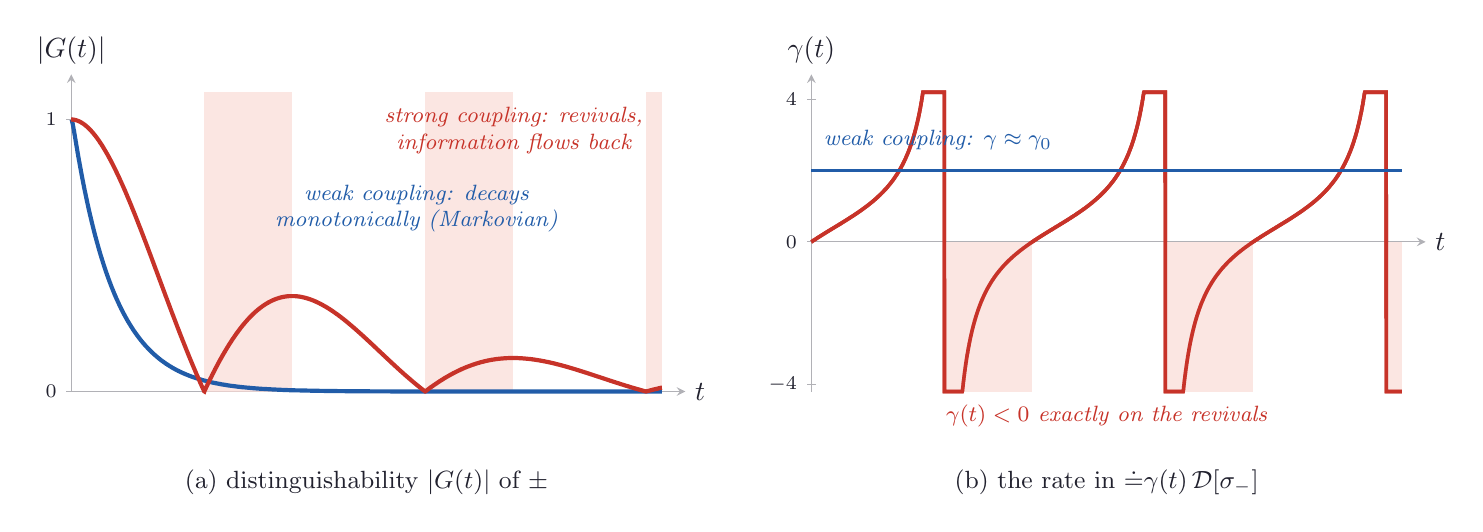
\begin{tikzpicture}[ink/.style={line width=0.9pt, ndInk}, faint/.style={line width=0.4pt, ndInk!35}, dashedink/.style={line width=0.5pt, ndInk!55, dash pattern=on 2.5pt off 2pt}, vec/.style={->, >=stealth, line width=1.2pt}, note/.style={font=\footnotesize\itshape, text=ndInk!85, align=center}, pointer/.style={->, >=stealth, line width=0.4pt, ndInk!60, shorten >=2pt, shorten <=1pt}, dot/.style={circle, fill=ndInk, inner sep=0pt, minimum size=3.4pt}, wash/.style={fill=ndSky, fill opacity=0.55}, every node/.style={text=ndInk}]
\definecolor{ndInk}{rgb}{0.13,0.13,0.18}
\definecolor{ndPaper}{rgb}{0.99,0.96,0.88}
\definecolor{ndSky}{rgb}{0.84,0.91,0.98}
\definecolor{ndRose}{rgb}{0.98,0.86,0.84}
\definecolor{ndBlue}{rgb}{0.13,0.36,0.66}
\definecolor{ndRed}{rgb}{0.78,0.20,0.16}
\definecolor{ndGold}{rgb}{0.88,0.62,0.10}
\definecolor{ndGreen}{rgb}{0.18,0.52,0.30}
\draw[faint, ->, >=stealth] (0.000,0.000) -- (7.800,0.000) node[right, text=ndInk] {$t$};
\draw[faint, ->, >=stealth] (0.000,0.000) -- (0.000,4.028) node[above, text=ndInk] {$|G(t)|$};
\draw[faint] (0.060,0.000) -- (-0.060,0.000) node[left, font=\scriptsize, text=ndInk] {$0$};
\draw[faint] (0.060,3.455) -- (-0.060,3.455) node[left, font=\scriptsize, text=ndInk] {$1$};
\fill[ndRose, fill opacity=0.7] (1.691,0.000) rectangle (2.803,3.800);
\fill[ndRose, fill opacity=0.7] (4.494,0.000) rectangle (5.608,3.800);
\fill[ndRose, fill opacity=0.7] (7.299,0.000) rectangle (7.497,3.800);
\draw[line width=1.5pt, ndBlue] (0.000,3.455) -- (0.003,3.453) -- (0.005,3.448) -- (0.008,3.442) -- (0.011,3.433) -- (0.013,3.423) -- (0.016,3.411) -- (0.019,3.399) -- (0.021,3.386) -- (0.024,3.372) -- (0.027,3.357) -- (0.029,3.342) -- (0.032,3.327) -- (0.035,3.312) -- (0.038,3.296) -- (0.040,3.280) -- (0.043,3.264) -- (0.046,3.248) -- (0.048,3.232) -- (0.051,3.216) -- (0.054,3.200) -- (0.056,3.184) -- (0.059,3.168) -- (0.062,3.152) -- (0.064,3.136) -- (0.067,3.120) -- (0.070,3.104) -- (0.072,3.088) -- (0.075,3.073) -- (0.078,3.057) -- (0.080,3.041) -- (0.083,3.026) -- (0.086,3.010) -- (0.088,2.995) -- (0.091,2.980) -- (0.094,2.964) -- (0.096,2.949) -- (0.099,2.934) -- (0.102,2.919) -- (0.105,2.904) -- (0.107,2.889) -- (0.110,2.875) -- (0.113,2.860) -- (0.115,2.845) -- (0.118,2.831) -- (0.121,2.816) -- (0.123,2.802) -- (0.126,2.787) -- (0.129,2.773) -- (0.131,2.759) -- (0.134,2.745) -- (0.137,2.731) -- (0.139,2.717) -- (0.142,2.703) -- (0.145,2.689) -- (0.147,2.675) -- (0.150,2.662) -- (0.153,2.648) -- (0.155,2.634) -- (0.158,2.621) -- (0.161,2.607) -- (0.163,2.594) -- (0.166,2.581) -- (0.169,2.568) -- (0.171,2.554) -- (0.174,2.541) -- (0.177,2.528) -- (0.180,2.515) -- (0.182,2.503) -- (0.185,2.490) -- (0.188,2.477) -- (0.190,2.464) -- (0.193,2.452) -- (0.196,2.439) -- (0.198,2.427) -- (0.201,2.414) -- (0.204,2.402) -- (0.206,2.390) -- (0.209,2.377) -- (0.212,2.365) -- (0.214,2.353) -- (0.217,2.341) -- (0.220,2.329) -- (0.222,2.317) -- (0.225,2.305) -- (0.228,2.293) -- (0.230,2.282) -- (0.233,2.270) -- (0.236,2.258) -- (0.238,2.247) -- (0.241,2.235) -- (0.244,2.224) -- (0.247,2.212) -- (0.249,2.201) -- (0.252,2.190) -- (0.255,2.179) -- (0.257,2.167) -- (0.260,2.156) -- (0.263,2.145) -- (0.265,2.134) -- (0.268,2.123) -- (0.271,2.113) -- (0.273,2.102) -- (0.276,2.091) -- (0.279,2.080) -- (0.281,2.070) -- (0.284,2.059) -- (0.287,2.048) -- (0.289,2.038) -- (0.292,2.028) -- (0.295,2.017) -- (0.297,2.007) -- (0.300,1.997) -- (0.303,1.986) -- (0.305,1.976) -- (0.308,1.966) -- (0.311,1.956) -- (0.314,1.946) -- (0.316,1.936) -- (0.319,1.926) -- (0.322,1.916) -- (0.324,1.906) -- (0.327,1.897) -- (0.330,1.887) -- (0.332,1.877) -- (0.335,1.868) -- (0.338,1.858) -- (0.340,1.849) -- (0.343,1.839) -- (0.346,1.830) -- (0.348,1.820) -- (0.351,1.811) -- (0.354,1.802) -- (0.356,1.793) -- (0.359,1.783) -- (0.362,1.774) -- (0.364,1.765) -- (0.367,1.756) -- (0.370,1.747) -- (0.372,1.738) -- (0.375,1.729) -- (0.378,1.720) -- (0.380,1.712) -- (0.383,1.703) -- (0.386,1.694) -- (0.389,1.685) -- (0.391,1.677) -- (0.394,1.668) -- (0.397,1.660) -- (0.399,1.651) -- (0.402,1.643) -- (0.405,1.634) -- (0.407,1.626) -- (0.410,1.618) -- (0.413,1.609) -- (0.415,1.601) -- (0.418,1.593) -- (0.421,1.585) -- (0.423,1.577) -- (0.426,1.569) -- (0.429,1.561) -- (0.431,1.553) -- (0.434,1.545) -- (0.437,1.537) -- (0.439,1.529) -- (0.442,1.521) -- (0.445,1.513) -- (0.447,1.505) -- (0.450,1.498) -- (0.453,1.490) -- (0.456,1.482) -- (0.458,1.475) -- (0.461,1.467) -- (0.464,1.460) -- (0.466,1.452) -- (0.469,1.445) -- (0.472,1.437) -- (0.474,1.430) -- (0.477,1.423) -- (0.480,1.415) -- (0.482,1.408) -- (0.485,1.401) -- (0.488,1.394) -- (0.490,1.387) -- (0.493,1.380) -- (0.496,1.373) -- (0.498,1.366) -- (0.501,1.359) -- (0.504,1.352) -- (0.506,1.345) -- (0.509,1.338) -- (0.512,1.331) -- (0.514,1.324) -- (0.517,1.317) -- (0.520,1.311) -- (0.523,1.304) -- (0.525,1.297) -- (0.528,1.291) -- (0.531,1.284) -- (0.533,1.277) -- (0.536,1.271) -- (0.539,1.264) -- (0.541,1.258) -- (0.544,1.251) -- (0.547,1.245) -- (0.549,1.239) -- (0.552,1.232) -- (0.555,1.226) -- (0.557,1.220) -- (0.560,1.213) -- (0.563,1.207) -- (0.565,1.201) -- (0.568,1.195) -- (0.571,1.189) -- (0.573,1.183) -- (0.576,1.177) -- (0.579,1.171) -- (0.581,1.165) -- (0.584,1.159) -- (0.587,1.153) -- (0.589,1.147) -- (0.592,1.141) -- (0.595,1.135) -- (0.598,1.129) -- (0.600,1.124) -- (0.603,1.118) -- (0.606,1.112) -- (0.608,1.106) -- (0.611,1.101) -- (0.614,1.095) -- (0.616,1.089) -- (0.619,1.084) -- (0.622,1.078) -- (0.624,1.073) -- (0.627,1.067) -- (0.630,1.062) -- (0.632,1.056) -- (0.635,1.051) -- (0.638,1.046) -- (0.640,1.040) -- (0.643,1.035) -- (0.646,1.030) -- (0.648,1.024) -- (0.651,1.019) -- (0.654,1.014) -- (0.656,1.009) -- (0.659,1.004) -- (0.662,0.998) -- (0.665,0.993) -- (0.667,0.988) -- (0.670,0.983) -- (0.673,0.978) -- (0.675,0.973) -- (0.678,0.968) -- (0.681,0.963) -- (0.683,0.958) -- (0.686,0.953) -- (0.689,0.948) -- (0.691,0.944) -- (0.694,0.939) -- (0.697,0.934) -- (0.699,0.929) -- (0.702,0.924) -- (0.705,0.920) -- (0.707,0.915) -- (0.710,0.910) -- (0.713,0.906) -- (0.715,0.901) -- (0.718,0.896) -- (0.721,0.892) -- (0.723,0.887) -- (0.726,0.883) -- (0.729,0.878) -- (0.732,0.874) -- (0.734,0.869) -- (0.737,0.865) -- (0.740,0.860) -- (0.742,0.856) -- (0.745,0.852) -- (0.748,0.847) -- (0.750,0.843) -- (0.753,0.839) -- (0.756,0.834) -- (0.758,0.830) -- (0.761,0.826) -- (0.764,0.821) -- (0.766,0.817) -- (0.769,0.813) -- (0.772,0.809) -- (0.774,0.805) -- (0.777,0.801) -- (0.780,0.797) -- (0.782,0.792) -- (0.785,0.788) -- (0.788,0.784) -- (0.790,0.780) -- (0.793,0.776) -- (0.796,0.772) -- (0.798,0.768) -- (0.801,0.764) -- (0.804,0.761) -- (0.807,0.757) -- (0.809,0.753) -- (0.812,0.749) -- (0.815,0.745) -- (0.817,0.741) -- (0.820,0.738) -- (0.823,0.734) -- (0.825,0.730) -- (0.828,0.726) -- (0.831,0.723) -- (0.833,0.719) -- (0.836,0.715) -- (0.839,0.711) -- (0.841,0.708) -- (0.844,0.704) -- (0.847,0.701) -- (0.849,0.697) -- (0.852,0.693) -- (0.855,0.690) -- (0.857,0.686) -- (0.860,0.683) -- (0.863,0.679) -- (0.865,0.676) -- (0.868,0.672) -- (0.871,0.669) -- (0.874,0.666) -- (0.876,0.662) -- (0.879,0.659) -- (0.882,0.655) -- (0.884,0.652) -- (0.887,0.649) -- (0.890,0.645) -- (0.892,0.642) -- (0.895,0.639) -- (0.898,0.635) -- (0.900,0.632) -- (0.903,0.629) -- (0.906,0.626) -- (0.908,0.623) -- (0.911,0.619) -- (0.914,0.616) -- (0.916,0.613) -- (0.919,0.610) -- (0.922,0.607) -- (0.924,0.604) -- (0.927,0.601) -- (0.930,0.598) -- (0.932,0.594) -- (0.935,0.591) -- (0.938,0.588) -- (0.941,0.585) -- (0.943,0.582) -- (0.946,0.579) -- (0.949,0.576) -- (0.951,0.573) -- (0.954,0.571) -- (0.957,0.568) -- (0.959,0.565) -- (0.962,0.562) -- (0.965,0.559) -- (0.967,0.556) -- (0.970,0.553) -- (0.973,0.550) -- (0.975,0.548) -- (0.978,0.545) -- (0.981,0.542) -- (0.983,0.539) -- (0.986,0.536) -- (0.989,0.534) -- (0.991,0.531) -- (0.994,0.528) -- (0.997,0.526) -- (0.999,0.523) -- (1.002,0.520) -- (1.005,0.518) -- (1.008,0.515) -- (1.010,0.512) -- (1.013,0.510) -- (1.016,0.507) -- (1.018,0.504) -- (1.021,0.502) -- (1.024,0.499) -- (1.026,0.497) -- (1.029,0.494) -- (1.032,0.492) -- (1.034,0.489) -- (1.037,0.487) -- (1.040,0.484) -- (1.042,0.482) -- (1.045,0.479) -- (1.048,0.477) -- (1.050,0.474) -- (1.053,0.472) -- (1.056,0.469) -- (1.058,0.467) -- (1.061,0.465) -- (1.064,0.462) -- (1.066,0.460) -- (1.069,0.458) -- (1.072,0.455) -- (1.074,0.453) -- (1.077,0.451) -- (1.080,0.448) -- (1.083,0.446) -- (1.085,0.444) -- (1.088,0.441) -- (1.091,0.439) -- (1.093,0.437) -- (1.096,0.435) -- (1.099,0.432) -- (1.101,0.430) -- (1.104,0.428) -- (1.107,0.426) -- (1.109,0.424) -- (1.112,0.421) -- (1.115,0.419) -- (1.117,0.417) -- (1.120,0.415) -- (1.123,0.413) -- (1.125,0.411) -- (1.128,0.409) -- (1.131,0.407) -- (1.133,0.405) -- (1.136,0.402) -- (1.139,0.400) -- (1.141,0.398) -- (1.144,0.396) -- (1.147,0.394) -- (1.150,0.392) -- (1.152,0.390) -- (1.155,0.388) -- (1.158,0.386) -- (1.160,0.384) -- (1.163,0.382) -- (1.166,0.380) -- (1.168,0.378) -- (1.171,0.376) -- (1.174,0.375) -- (1.176,0.373) -- (1.179,0.371) -- (1.182,0.369) -- (1.184,0.367) -- (1.187,0.365) -- (1.190,0.363) -- (1.192,0.361) -- (1.195,0.359) -- (1.198,0.358) -- (1.200,0.356) -- (1.203,0.354) -- (1.206,0.352) -- (1.208,0.350) -- (1.211,0.349) -- (1.214,0.347) -- (1.217,0.345) -- (1.219,0.343) -- (1.222,0.341) -- (1.225,0.340) -- (1.227,0.338) -- (1.230,0.336) -- (1.233,0.335) -- (1.235,0.333) -- (1.238,0.331) -- (1.241,0.329) -- (1.243,0.328) -- (1.246,0.326) -- (1.249,0.324) -- (1.251,0.323) -- (1.254,0.321) -- (1.257,0.319) -- (1.259,0.318) -- (1.262,0.316) -- (1.265,0.315) -- (1.267,0.313) -- (1.270,0.311) -- (1.273,0.310) -- (1.275,0.308) -- (1.278,0.307) -- (1.281,0.305) -- (1.283,0.303) -- (1.286,0.302) -- (1.289,0.300) -- (1.292,0.299) -- (1.294,0.297) -- (1.297,0.296) -- (1.300,0.294) -- (1.302,0.293) -- (1.305,0.291) -- (1.308,0.290) -- (1.310,0.288) -- (1.313,0.287) -- (1.316,0.285) -- (1.318,0.284) -- (1.321,0.282) -- (1.324,0.281) -- (1.326,0.280) -- (1.329,0.278) -- (1.332,0.277) -- (1.334,0.275) -- (1.337,0.274) -- (1.340,0.272) -- (1.342,0.271) -- (1.345,0.270) -- (1.348,0.268) -- (1.350,0.267) -- (1.353,0.266) -- (1.356,0.264) -- (1.359,0.263) -- (1.361,0.261) -- (1.364,0.260) -- (1.367,0.259) -- (1.369,0.257) -- (1.372,0.256) -- (1.375,0.255) -- (1.377,0.254) -- (1.380,0.252) -- (1.383,0.251) -- (1.385,0.250) -- (1.388,0.248) -- (1.391,0.247) -- (1.393,0.246) -- (1.396,0.245) -- (1.399,0.243) -- (1.401,0.242) -- (1.404,0.241) -- (1.407,0.240) -- (1.409,0.238) -- (1.412,0.237) -- (1.415,0.236) -- (1.417,0.235) -- (1.420,0.234) -- (1.423,0.232) -- (1.426,0.231) -- (1.428,0.230) -- (1.431,0.229) -- (1.434,0.228) -- (1.436,0.226) -- (1.439,0.225) -- (1.442,0.224) -- (1.444,0.223) -- (1.447,0.222) -- (1.450,0.221) -- (1.452,0.220) -- (1.455,0.218) -- (1.458,0.217) -- (1.460,0.216) -- (1.463,0.215) -- (1.466,0.214) -- (1.468,0.213) -- (1.471,0.212) -- (1.474,0.211) -- (1.476,0.210) -- (1.479,0.209) -- (1.482,0.208) -- (1.484,0.206) -- (1.487,0.205) -- (1.490,0.204) -- (1.492,0.203) -- (1.495,0.202) -- (1.498,0.201) -- (1.501,0.200) -- (1.503,0.199) -- (1.506,0.198) -- (1.509,0.197) -- (1.511,0.196) -- (1.514,0.195) -- (1.517,0.194) -- (1.519,0.193) -- (1.522,0.192) -- (1.525,0.191) -- (1.527,0.190) -- (1.530,0.189) -- (1.533,0.188) -- (1.535,0.187) -- (1.538,0.186) -- (1.541,0.185) -- (1.543,0.184) -- (1.546,0.183) -- (1.549,0.183) -- (1.551,0.182) -- (1.554,0.181) -- (1.557,0.180) -- (1.559,0.179) -- (1.562,0.178) -- (1.565,0.177) -- (1.568,0.176) -- (1.570,0.175) -- (1.573,0.174) -- (1.576,0.173) -- (1.578,0.173) -- (1.581,0.172) -- (1.584,0.171) -- (1.586,0.170) -- (1.589,0.169) -- (1.592,0.168) -- (1.594,0.167) -- (1.597,0.166) -- (1.600,0.166) -- (1.602,0.165) -- (1.605,0.164) -- (1.608,0.163) -- (1.610,0.162) -- (1.613,0.161) -- (1.616,0.161) -- (1.618,0.160) -- (1.621,0.159) -- (1.624,0.158) -- (1.626,0.157) -- (1.629,0.156) -- (1.632,0.156) -- (1.635,0.155) -- (1.637,0.154) -- (1.640,0.153) -- (1.643,0.153) -- (1.645,0.152) -- (1.648,0.151) -- (1.651,0.150) -- (1.653,0.149) -- (1.656,0.149) -- (1.659,0.148) -- (1.661,0.147) -- (1.664,0.146) -- (1.667,0.146) -- (1.669,0.145) -- (1.672,0.144) -- (1.675,0.143) -- (1.677,0.143) -- (1.680,0.142) -- (1.683,0.141) -- (1.685,0.140) -- (1.688,0.140) -- (1.691,0.139) -- (1.693,0.138) -- (1.696,0.138) -- (1.699,0.137) -- (1.702,0.136) -- (1.704,0.136) -- (1.707,0.135) -- (1.710,0.134) -- (1.712,0.133) -- (1.715,0.133) -- (1.718,0.132) -- (1.720,0.131) -- (1.723,0.131) -- (1.726,0.130) -- (1.728,0.129) -- (1.731,0.129) -- (1.734,0.128) -- (1.736,0.127) -- (1.739,0.127) -- (1.742,0.126) -- (1.744,0.125) -- (1.747,0.125) -- (1.750,0.124) -- (1.752,0.124) -- (1.755,0.123) -- (1.758,0.122) -- (1.760,0.122) -- (1.763,0.121) -- (1.766,0.120) -- (1.768,0.120) -- (1.771,0.119) -- (1.774,0.119) -- (1.777,0.118) -- (1.779,0.117) -- (1.782,0.117) -- (1.785,0.116) -- (1.787,0.116) -- (1.790,0.115) -- (1.793,0.114) -- (1.795,0.114) -- (1.798,0.113) -- (1.801,0.113) -- (1.803,0.112) -- (1.806,0.112) -- (1.809,0.111) -- (1.811,0.110) -- (1.814,0.110) -- (1.817,0.109) -- (1.819,0.109) -- (1.822,0.108) -- (1.825,0.108) -- (1.827,0.107) -- (1.830,0.106) -- (1.833,0.106) -- (1.835,0.105) -- (1.838,0.105) -- (1.841,0.104) -- (1.844,0.104) -- (1.846,0.103) -- (1.849,0.103) -- (1.852,0.102) -- (1.854,0.102) -- (1.857,0.101) -- (1.860,0.101) -- (1.862,0.100) -- (1.865,0.100) -- (1.868,0.099) -- (1.870,0.099) -- (1.873,0.098) -- (1.876,0.098) -- (1.878,0.097) -- (1.881,0.097) -- (1.884,0.096) -- (1.886,0.096) -- (1.889,0.095) -- (1.892,0.095) -- (1.894,0.094) -- (1.897,0.094) -- (1.900,0.093) -- (1.902,0.093) -- (1.905,0.092) -- (1.908,0.092) -- (1.911,0.091) -- (1.913,0.091) -- (1.916,0.090) -- (1.919,0.090) -- (1.921,0.089) -- (1.924,0.089) -- (1.927,0.089) -- (1.929,0.088) -- (1.932,0.088) -- (1.935,0.087) -- (1.937,0.087) -- (1.940,0.086) -- (1.943,0.086) -- (1.945,0.085) -- (1.948,0.085) -- (1.951,0.085) -- (1.953,0.084) -- (1.956,0.084) -- (1.959,0.083) -- (1.961,0.083) -- (1.964,0.082) -- (1.967,0.082) -- (1.969,0.082) -- (1.972,0.081) -- (1.975,0.081) -- (1.977,0.080) -- (1.980,0.080) -- (1.983,0.079) -- (1.986,0.079) -- (1.988,0.079) -- (1.991,0.078) -- (1.994,0.078) -- (1.996,0.077) -- (1.999,0.077) -- (2.002,0.077) -- (2.004,0.076) -- (2.007,0.076) -- (2.010,0.075) -- (2.012,0.075) -- (2.015,0.075) -- (2.018,0.074) -- (2.020,0.074) -- (2.023,0.074) -- (2.026,0.073) -- (2.028,0.073) -- (2.031,0.072) -- (2.034,0.072) -- (2.036,0.072) -- (2.039,0.071) -- (2.042,0.071) -- (2.044,0.071) -- (2.047,0.070) -- (2.050,0.070) -- (2.053,0.070) -- (2.055,0.069) -- (2.058,0.069) -- (2.061,0.068) -- (2.063,0.068) -- (2.066,0.068) -- (2.069,0.067) -- (2.071,0.067) -- (2.074,0.067) -- (2.077,0.066) -- (2.079,0.066) -- (2.082,0.066) -- (2.085,0.065) -- (2.087,0.065) -- (2.090,0.065) -- (2.093,0.064) -- (2.095,0.064) -- (2.098,0.064) -- (2.101,0.063) -- (2.103,0.063) -- (2.106,0.063) -- (2.109,0.062) -- (2.111,0.062) -- (2.114,0.062) -- (2.117,0.061) -- (2.120,0.061) -- (2.122,0.061) -- (2.125,0.061) -- (2.128,0.060) -- (2.130,0.060) -- (2.133,0.060) -- (2.136,0.059) -- (2.138,0.059) -- (2.141,0.059) -- (2.144,0.058) -- (2.146,0.058) -- (2.149,0.058) -- (2.152,0.058) -- (2.154,0.057) -- (2.157,0.057) -- (2.160,0.057) -- (2.162,0.056) -- (2.165,0.056) -- (2.168,0.056) -- (2.170,0.055) -- (2.173,0.055) -- (2.176,0.055) -- (2.178,0.055) -- (2.181,0.054) -- (2.184,0.054) -- (2.186,0.054) -- (2.189,0.054) -- (2.192,0.053) -- (2.195,0.053) -- (2.197,0.053) -- (2.200,0.052) -- (2.203,0.052) -- (2.205,0.052) -- (2.208,0.052) -- (2.211,0.051) -- (2.213,0.051) -- (2.216,0.051) -- (2.219,0.051) -- (2.221,0.050) -- (2.224,0.050) -- (2.227,0.050) -- (2.229,0.050) -- (2.232,0.049) -- (2.235,0.049) -- (2.237,0.049) -- (2.240,0.049) -- (2.243,0.048) -- (2.245,0.048) -- (2.248,0.048) -- (2.251,0.048) -- (2.253,0.047) -- (2.256,0.047) -- (2.259,0.047) -- (2.262,0.047) -- (2.264,0.046) -- (2.267,0.046) -- (2.270,0.046) -- (2.272,0.046) -- (2.275,0.045) -- (2.278,0.045) -- (2.280,0.045) -- (2.283,0.045) -- (2.286,0.044) -- (2.288,0.044) -- (2.291,0.044) -- (2.294,0.044) -- (2.296,0.044) -- (2.299,0.043) -- (2.302,0.043) -- (2.304,0.043) -- (2.307,0.043) -- (2.310,0.042) -- (2.312,0.042) -- (2.315,0.042) -- (2.318,0.042) -- (2.320,0.042) -- (2.323,0.041) -- (2.326,0.041) -- (2.329,0.041) -- (2.331,0.041) -- (2.334,0.041) -- (2.337,0.040) -- (2.339,0.040) -- (2.342,0.040) -- (2.345,0.040) -- (2.347,0.040) -- (2.350,0.039) -- (2.353,0.039) -- (2.355,0.039) -- (2.358,0.039) -- (2.361,0.039) -- (2.363,0.038) -- (2.366,0.038) -- (2.369,0.038) -- (2.371,0.038) -- (2.374,0.038) -- (2.377,0.037) -- (2.379,0.037) -- (2.382,0.037) -- (2.385,0.037) -- (2.387,0.037) -- (2.390,0.036) -- (2.393,0.036) -- (2.395,0.036) -- (2.398,0.036) -- (2.401,0.036) -- (2.404,0.035) -- (2.406,0.035) -- (2.409,0.035) -- (2.412,0.035) -- (2.414,0.035) -- (2.417,0.035) -- (2.420,0.034) -- (2.422,0.034) -- (2.425,0.034) -- (2.428,0.034) -- (2.430,0.034) -- (2.433,0.034) -- (2.436,0.033) -- (2.438,0.033) -- (2.441,0.033) -- (2.444,0.033) -- (2.446,0.033) -- (2.449,0.033) -- (2.452,0.032) -- (2.454,0.032) -- (2.457,0.032) -- (2.460,0.032) -- (2.462,0.032) -- (2.465,0.032) -- (2.468,0.031) -- (2.471,0.031) -- (2.473,0.031) -- (2.476,0.031) -- (2.479,0.031) -- (2.481,0.031) -- (2.484,0.030) -- (2.487,0.030) -- (2.489,0.030) -- (2.492,0.030) -- (2.495,0.030) -- (2.497,0.030) -- (2.500,0.030) -- (2.503,0.029) -- (2.505,0.029) -- (2.508,0.029) -- (2.511,0.029) -- (2.513,0.029) -- (2.516,0.029) -- (2.519,0.028) -- (2.521,0.028) -- (2.524,0.028) -- (2.527,0.028) -- (2.529,0.028) -- (2.532,0.028) -- (2.535,0.028) -- (2.538,0.027) -- (2.540,0.027) -- (2.543,0.027) -- (2.546,0.027) -- (2.548,0.027) -- (2.551,0.027) -- (2.554,0.027) -- (2.556,0.026) -- (2.559,0.026) -- (2.562,0.026) -- (2.564,0.026) -- (2.567,0.026) -- (2.570,0.026) -- (2.572,0.026) -- (2.575,0.026) -- (2.578,0.025) -- (2.580,0.025) -- (2.583,0.025) -- (2.586,0.025) -- (2.588,0.025) -- (2.591,0.025) -- (2.594,0.025) -- (2.596,0.025) -- (2.599,0.024) -- (2.602,0.024) -- (2.605,0.024) -- (2.607,0.024) -- (2.610,0.024) -- (2.613,0.024) -- (2.615,0.024) -- (2.618,0.024) -- (2.621,0.023) -- (2.623,0.023) -- (2.626,0.023) -- (2.629,0.023) -- (2.631,0.023) -- (2.634,0.023) -- (2.637,0.023) -- (2.639,0.023) -- (2.642,0.022) -- (2.645,0.022) -- (2.647,0.022) -- (2.650,0.022) -- (2.653,0.022) -- (2.655,0.022) -- (2.658,0.022) -- (2.661,0.022) -- (2.663,0.022) -- (2.666,0.021) -- (2.669,0.021) -- (2.671,0.021) -- (2.674,0.021) -- (2.677,0.021) -- (2.680,0.021) -- (2.682,0.021) -- (2.685,0.021) -- (2.688,0.021) -- (2.690,0.020) -- (2.693,0.020) -- (2.696,0.020) -- (2.698,0.020) -- (2.701,0.020) -- (2.704,0.020) -- (2.706,0.020) -- (2.709,0.020) -- (2.712,0.020) -- (2.714,0.020) -- (2.717,0.019) -- (2.720,0.019) -- (2.722,0.019) -- (2.725,0.019) -- (2.728,0.019) -- (2.730,0.019) -- (2.733,0.019) -- (2.736,0.019) -- (2.738,0.019) -- (2.741,0.019) -- (2.744,0.018) -- (2.747,0.018) -- (2.749,0.018) -- (2.752,0.018) -- (2.755,0.018) -- (2.757,0.018) -- (2.760,0.018) -- (2.763,0.018) -- (2.765,0.018) -- (2.768,0.018) -- (2.771,0.018) -- (2.773,0.017) -- (2.776,0.017) -- (2.779,0.017) -- (2.781,0.017) -- (2.784,0.017) -- (2.787,0.017) -- (2.789,0.017) -- (2.792,0.017) -- (2.795,0.017) -- (2.797,0.017) -- (2.800,0.017) -- (2.803,0.017) -- (2.805,0.016) -- (2.808,0.016) -- (2.811,0.016) -- (2.814,0.016) -- (2.816,0.016) -- (2.819,0.016) -- (2.822,0.016) -- (2.824,0.016) -- (2.827,0.016) -- (2.830,0.016) -- (2.832,0.016) -- (2.835,0.016) -- (2.838,0.015) -- (2.840,0.015) -- (2.843,0.015) -- (2.846,0.015) -- (2.848,0.015) -- (2.851,0.015) -- (2.854,0.015) -- (2.856,0.015) -- (2.859,0.015) -- (2.862,0.015) -- (2.864,0.015) -- (2.867,0.015) -- (2.870,0.015) -- (2.872,0.014) -- (2.875,0.014) -- (2.878,0.014) -- (2.880,0.014) -- (2.883,0.014) -- (2.886,0.014) -- (2.889,0.014) -- (2.891,0.014) -- (2.894,0.014) -- (2.897,0.014) -- (2.899,0.014) -- (2.902,0.014) -- (2.905,0.014) -- (2.907,0.014) -- (2.910,0.013) -- (2.913,0.013) -- (2.915,0.013) -- (2.918,0.013) -- (2.921,0.013) -- (2.923,0.013) -- (2.926,0.013) -- (2.929,0.013) -- (2.931,0.013) -- (2.934,0.013) -- (2.937,0.013) -- (2.939,0.013) -- (2.942,0.013) -- (2.945,0.013) -- (2.947,0.013) -- (2.950,0.012) -- (2.953,0.012) -- (2.956,0.012) -- (2.958,0.012) -- (2.961,0.012) -- (2.964,0.012) -- (2.966,0.012) -- (2.969,0.012) -- (2.972,0.012) -- (2.974,0.012) -- (2.977,0.012) -- (2.980,0.012) -- (2.982,0.012) -- (2.985,0.012) -- (2.988,0.012) -- (2.990,0.012) -- (2.993,0.011) -- (2.996,0.011) -- (2.998,0.011) -- (3.001,0.011) -- (3.004,0.011) -- (3.006,0.011) -- (3.009,0.011) -- (3.012,0.011) -- (3.014,0.011) -- (3.017,0.011) -- (3.020,0.011) -- (3.023,0.011) -- (3.025,0.011) -- (3.028,0.011) -- (3.031,0.011) -- (3.033,0.011) -- (3.036,0.011) -- (3.039,0.011) -- (3.041,0.010) -- (3.044,0.010) -- (3.047,0.010) -- (3.049,0.010) -- (3.052,0.010) -- (3.055,0.010) -- (3.057,0.010) -- (3.060,0.010) -- (3.063,0.010) -- (3.065,0.010) -- (3.068,0.010) -- (3.071,0.010) -- (3.073,0.010) -- (3.076,0.010) -- (3.079,0.010) -- (3.081,0.010) -- (3.084,0.010) -- (3.087,0.010) -- (3.089,0.010) -- (3.092,0.009) -- (3.095,0.009) -- (3.098,0.009) -- (3.100,0.009) -- (3.103,0.009) -- (3.106,0.009) -- (3.108,0.009) -- (3.111,0.009) -- (3.114,0.009) -- (3.116,0.009) -- (3.119,0.009) -- (3.122,0.009) -- (3.124,0.009) -- (3.127,0.009) -- (3.130,0.009) -- (3.132,0.009) -- (3.135,0.009) -- (3.138,0.009) -- (3.140,0.009) -- (3.143,0.009) -- (3.146,0.009) -- (3.148,0.009) -- (3.151,0.008) -- (3.154,0.008) -- (3.156,0.008) -- (3.159,0.008) -- (3.162,0.008) -- (3.165,0.008) -- (3.167,0.008) -- (3.170,0.008) -- (3.173,0.008) -- (3.175,0.008) -- (3.178,0.008) -- (3.181,0.008) -- (3.183,0.008) -- (3.186,0.008) -- (3.189,0.008) -- (3.191,0.008) -- (3.194,0.008) -- (3.197,0.008) -- (3.199,0.008) -- (3.202,0.008) -- (3.205,0.008) -- (3.207,0.008) -- (3.210,0.008) -- (3.213,0.008) -- (3.215,0.007) -- (3.218,0.007) -- (3.221,0.007) -- (3.223,0.007) -- (3.226,0.007) -- (3.229,0.007) -- (3.232,0.007) -- (3.234,0.007) -- (3.237,0.007) -- (3.240,0.007) -- (3.242,0.007) -- (3.245,0.007) -- (3.248,0.007) -- (3.250,0.007) -- (3.253,0.007) -- (3.256,0.007) -- (3.258,0.007) -- (3.261,0.007) -- (3.264,0.007) -- (3.266,0.007) -- (3.269,0.007) -- (3.272,0.007) -- (3.274,0.007) -- (3.277,0.007) -- (3.280,0.007) -- (3.282,0.007) -- (3.285,0.007) -- (3.288,0.007) -- (3.290,0.006) -- (3.293,0.006) -- (3.296,0.006) -- (3.298,0.006) -- (3.301,0.006) -- (3.304,0.006) -- (3.307,0.006) -- (3.309,0.006) -- (3.312,0.006) -- (3.315,0.006) -- (3.317,0.006) -- (3.320,0.006) -- (3.323,0.006) -- (3.325,0.006) -- (3.328,0.006) -- (3.331,0.006) -- (3.333,0.006) -- (3.336,0.006) -- (3.339,0.006) -- (3.341,0.006) -- (3.344,0.006) -- (3.347,0.006) -- (3.349,0.006) -- (3.352,0.006) -- (3.355,0.006) -- (3.357,0.006) -- (3.360,0.006) -- (3.363,0.006) -- (3.365,0.006) -- (3.368,0.006) -- (3.371,0.006) -- (3.374,0.006) -- (3.376,0.006) -- (3.379,0.005) -- (3.382,0.005) -- (3.384,0.005) -- (3.387,0.005) -- (3.390,0.005) -- (3.392,0.005) -- (3.395,0.005) -- (3.398,0.005) -- (3.400,0.005) -- (3.403,0.005) -- (3.406,0.005) -- (3.408,0.005) -- (3.411,0.005) -- (3.414,0.005) -- (3.416,0.005) -- (3.419,0.005) -- (3.422,0.005) -- (3.424,0.005) -- (3.427,0.005) -- (3.430,0.005) -- (3.432,0.005) -- (3.435,0.005) -- (3.438,0.005) -- (3.441,0.005) -- (3.443,0.005) -- (3.446,0.005) -- (3.449,0.005) -- (3.451,0.005) -- (3.454,0.005) -- (3.457,0.005) -- (3.459,0.005) -- (3.462,0.005) -- (3.465,0.005) -- (3.467,0.005) -- (3.470,0.005) -- (3.473,0.005) -- (3.475,0.005) -- (3.478,0.005) -- (3.481,0.005) -- (3.483,0.004) -- (3.486,0.004) -- (3.489,0.004) -- (3.491,0.004) -- (3.494,0.004) -- (3.497,0.004) -- (3.499,0.004) -- (3.502,0.004) -- (3.505,0.004) -- (3.508,0.004) -- (3.510,0.004) -- (3.513,0.004) -- (3.516,0.004) -- (3.518,0.004) -- (3.521,0.004) -- (3.524,0.004) -- (3.526,0.004) -- (3.529,0.004) -- (3.532,0.004) -- (3.534,0.004) -- (3.537,0.004) -- (3.540,0.004) -- (3.542,0.004) -- (3.545,0.004) -- (3.548,0.004) -- (3.550,0.004) -- (3.553,0.004) -- (3.556,0.004) -- (3.558,0.004) -- (3.561,0.004) -- (3.564,0.004) -- (3.566,0.004) -- (3.569,0.004) -- (3.572,0.004) -- (3.574,0.004) -- (3.577,0.004) -- (3.580,0.004) -- (3.583,0.004) -- (3.585,0.004) -- (3.588,0.004) -- (3.591,0.004) -- (3.593,0.004) -- (3.596,0.004) -- (3.599,0.004) -- (3.601,0.004) -- (3.604,0.004) -- (3.607,0.004) -- (3.609,0.004) -- (3.612,0.004) -- (3.615,0.003) -- (3.617,0.003) -- (3.620,0.003) -- (3.623,0.003) -- (3.625,0.003) -- (3.628,0.003) -- (3.631,0.003) -- (3.633,0.003) -- (3.636,0.003) -- (3.639,0.003) -- (3.641,0.003) -- (3.644,0.003) -- (3.647,0.003) -- (3.650,0.003) -- (3.652,0.003) -- (3.655,0.003) -- (3.658,0.003) -- (3.660,0.003) -- (3.663,0.003) -- (3.666,0.003) -- (3.668,0.003) -- (3.671,0.003) -- (3.674,0.003) -- (3.676,0.003) -- (3.679,0.003) -- (3.682,0.003) -- (3.684,0.003) -- (3.687,0.003) -- (3.690,0.003) -- (3.692,0.003) -- (3.695,0.003) -- (3.698,0.003) -- (3.700,0.003) -- (3.703,0.003) -- (3.706,0.003) -- (3.708,0.003) -- (3.711,0.003) -- (3.714,0.003) -- (3.717,0.003) -- (3.719,0.003) -- (3.722,0.003) -- (3.725,0.003) -- (3.727,0.003) -- (3.730,0.003) -- (3.733,0.003) -- (3.735,0.003) -- (3.738,0.003) -- (3.741,0.003) -- (3.743,0.003) -- (3.746,0.003) -- (3.749,0.003) -- (3.751,0.003) -- (3.754,0.003) -- (3.757,0.003) -- (3.759,0.003) -- (3.762,0.003) -- (3.765,0.003) -- (3.767,0.003) -- (3.770,0.003) -- (3.773,0.003) -- (3.775,0.003) -- (3.778,0.003) -- (3.781,0.003) -- (3.783,0.003) -- (3.786,0.003) -- (3.789,0.002) -- (3.792,0.002) -- (3.794,0.002) -- (3.797,0.002) -- (3.800,0.002) -- (3.802,0.002) -- (3.805,0.002) -- (3.808,0.002) -- (3.810,0.002) -- (3.813,0.002) -- (3.816,0.002) -- (3.818,0.002) -- (3.821,0.002) -- (3.824,0.002) -- (3.826,0.002) -- (3.829,0.002) -- (3.832,0.002) -- (3.834,0.002) -- (3.837,0.002) -- (3.840,0.002) -- (3.842,0.002) -- (3.845,0.002) -- (3.848,0.002) -- (3.850,0.002) -- (3.853,0.002) -- (3.856,0.002) -- (3.859,0.002) -- (3.861,0.002) -- (3.864,0.002) -- (3.867,0.002) -- (3.869,0.002) -- (3.872,0.002) -- (3.875,0.002) -- (3.877,0.002) -- (3.880,0.002) -- (3.883,0.002) -- (3.885,0.002) -- (3.888,0.002) -- (3.891,0.002) -- (3.893,0.002) -- (3.896,0.002) -- (3.899,0.002) -- (3.901,0.002) -- (3.904,0.002) -- (3.907,0.002) -- (3.909,0.002) -- (3.912,0.002) -- (3.915,0.002) -- (3.917,0.002) -- (3.920,0.002) -- (3.923,0.002) -- (3.926,0.002) -- (3.928,0.002) -- (3.931,0.002) -- (3.934,0.002) -- (3.936,0.002) -- (3.939,0.002) -- (3.942,0.002) -- (3.944,0.002) -- (3.947,0.002) -- (3.950,0.002) -- (3.952,0.002) -- (3.955,0.002) -- (3.958,0.002) -- (3.960,0.002) -- (3.963,0.002) -- (3.966,0.002) -- (3.968,0.002) -- (3.971,0.002) -- (3.974,0.002) -- (3.976,0.002) -- (3.979,0.002) -- (3.982,0.002) -- (3.984,0.002) -- (3.987,0.002) -- (3.990,0.002) -- (3.992,0.002) -- (3.995,0.002) -- (3.998,0.002) -- (4.001,0.002) -- (4.003,0.002) -- (4.006,0.002) -- (4.009,0.002) -- (4.011,0.002) -- (4.014,0.002) -- (4.017,0.002) -- (4.019,0.002) -- (4.022,0.002) -- (4.025,0.002) -- (4.027,0.002) -- (4.030,0.002) -- (4.033,0.002) -- (4.035,0.002) -- (4.038,0.002) -- (4.041,0.002) -- (4.043,0.002) -- (4.046,0.002) -- (4.049,0.002) -- (4.051,0.002) -- (4.054,0.002) -- (4.057,0.001) -- (4.059,0.001) -- (4.062,0.001) -- (4.065,0.001) -- (4.068,0.001) -- (4.070,0.001) -- (4.073,0.001) -- (4.076,0.001) -- (4.078,0.001) -- (4.081,0.001) -- (4.084,0.001) -- (4.086,0.001) -- (4.089,0.001) -- (4.092,0.001) -- (4.094,0.001) -- (4.097,0.001) -- (4.100,0.001) -- (4.102,0.001) -- (4.105,0.001) -- (4.108,0.001) -- (4.110,0.001) -- (4.113,0.001) -- (4.116,0.001) -- (4.118,0.001) -- (4.121,0.001) -- (4.124,0.001) -- (4.126,0.001) -- (4.129,0.001) -- (4.132,0.001) -- (4.135,0.001) -- (4.137,0.001) -- (4.140,0.001) -- (4.143,0.001) -- (4.145,0.001) -- (4.148,0.001) -- (4.151,0.001) -- (4.153,0.001) -- (4.156,0.001) -- (4.159,0.001) -- (4.161,0.001) -- (4.164,0.001) -- (4.167,0.001) -- (4.169,0.001) -- (4.172,0.001) -- (4.175,0.001) -- (4.177,0.001) -- (4.180,0.001) -- (4.183,0.001) -- (4.185,0.001) -- (4.188,0.001) -- (4.191,0.001) -- (4.193,0.001) -- (4.196,0.001) -- (4.199,0.001) -- (4.202,0.001) -- (4.204,0.001) -- (4.207,0.001) -- (4.210,0.001) -- (4.212,0.001) -- (4.215,0.001) -- (4.218,0.001) -- (4.220,0.001) -- (4.223,0.001) -- (4.226,0.001) -- (4.228,0.001) -- (4.231,0.001) -- (4.234,0.001) -- (4.236,0.001) -- (4.239,0.001) -- (4.242,0.001) -- (4.244,0.001) -- (4.247,0.001) -- (4.250,0.001) -- (4.252,0.001) -- (4.255,0.001) -- (4.258,0.001) -- (4.260,0.001) -- (4.263,0.001) -- (4.266,0.001) -- (4.268,0.001) -- (4.271,0.001) -- (4.274,0.001) -- (4.277,0.001) -- (4.279,0.001) -- (4.282,0.001) -- (4.285,0.001) -- (4.287,0.001) -- (4.290,0.001) -- (4.293,0.001) -- (4.295,0.001) -- (4.298,0.001) -- (4.301,0.001) -- (4.303,0.001) -- (4.306,0.001) -- (4.309,0.001) -- (4.311,0.001) -- (4.314,0.001) -- (4.317,0.001) -- (4.319,0.001) -- (4.322,0.001) -- (4.325,0.001) -- (4.327,0.001) -- (4.330,0.001) -- (4.333,0.001) -- (4.335,0.001) -- (4.338,0.001) -- (4.341,0.001) -- (4.344,0.001) -- (4.346,0.001) -- (4.349,0.001) -- (4.352,0.001) -- (4.354,0.001) -- (4.357,0.001) -- (4.360,0.001) -- (4.362,0.001) -- (4.365,0.001) -- (4.368,0.001) -- (4.370,0.001) -- (4.373,0.001) -- (4.376,0.001) -- (4.378,0.001) -- (4.381,0.001) -- (4.384,0.001) -- (4.386,0.001) -- (4.389,0.001) -- (4.392,0.001) -- (4.394,0.001) -- (4.397,0.001) -- (4.400,0.001) -- (4.402,0.001) -- (4.405,0.001) -- (4.408,0.001) -- (4.411,0.001) -- (4.413,0.001) -- (4.416,0.001) -- (4.419,0.001) -- (4.421,0.001) -- (4.424,0.001) -- (4.427,0.001) -- (4.429,0.001) -- (4.432,0.001) -- (4.435,0.001) -- (4.437,0.001) -- (4.440,0.001) -- (4.443,0.001) -- (4.445,0.001) -- (4.448,0.001) -- (4.451,0.001) -- (4.453,0.001) -- (4.456,0.001) -- (4.459,0.001) -- (4.461,0.001) -- (4.464,0.001) -- (4.467,0.001) -- (4.469,0.001) -- (4.472,0.001) -- (4.475,0.001) -- (4.477,0.001) -- (4.480,0.001) -- (4.483,0.001) -- (4.486,0.001) -- (4.488,0.001) -- (4.491,0.001) -- (4.494,0.001) -- (4.496,0.001) -- (4.499,0.001) -- (4.502,0.001) -- (4.504,0.001) -- (4.507,0.001) -- (4.510,0.001) -- (4.512,0.001) -- (4.515,0.001) -- (4.518,0.001) -- (4.520,0.001) -- (4.523,0.001) -- (4.526,0.001) -- (4.528,0.001) -- (4.531,0.001) -- (4.534,0.001) -- (4.536,0.001) -- (4.539,0.001) -- (4.542,0.001) -- (4.544,0.001) -- (4.547,0.001) -- (4.550,0.001) -- (4.553,0.001) -- (4.555,0.001) -- (4.558,0.001) -- (4.561,0.001) -- (4.563,0.001) -- (4.566,0.001) -- (4.569,0.001) -- (4.571,0.001) -- (4.574,0.001) -- (4.577,0.001) -- (4.579,0.001) -- (4.582,0.001) -- (4.585,0.001) -- (4.587,0.001) -- (4.590,0.001) -- (4.593,0.001) -- (4.595,0.001) -- (4.598,0.001) -- (4.601,0.001) -- (4.603,0.001) -- (4.606,0.001) -- (4.609,0.001) -- (4.611,0.001) -- (4.614,0.001) -- (4.617,0.001) -- (4.620,0.001) -- (4.622,0.001) -- (4.625,0.001) -- (4.628,0.001) -- (4.630,0.000) -- (4.633,0.000) -- (4.636,0.000) -- (4.638,0.000) -- (4.641,0.000) -- (4.644,0.000) -- (4.646,0.000) -- (4.649,0.000) -- (4.652,0.000) -- (4.654,0.000) -- (4.657,0.000) -- (4.660,0.000) -- (4.662,0.000) -- (4.665,0.000) -- (4.668,0.000) -- (4.670,0.000) -- (4.673,0.000) -- (4.676,0.000) -- (4.678,0.000) -- (4.681,0.000) -- (4.684,0.000) -- (4.686,0.000) -- (4.689,0.000) -- (4.692,0.000) -- (4.695,0.000) -- (4.697,0.000) -- (4.700,0.000) -- (4.703,0.000) -- (4.705,0.000) -- (4.708,0.000) -- (4.711,0.000) -- (4.713,0.000) -- (4.716,0.000) -- (4.719,0.000) -- (4.721,0.000) -- (4.724,0.000) -- (4.727,0.000) -- (4.729,0.000) -- (4.732,0.000) -- (4.735,0.000) -- (4.737,0.000) -- (4.740,0.000) -- (4.743,0.000) -- (4.745,0.000) -- (4.748,0.000) -- (4.751,0.000) -- (4.753,0.000) -- (4.756,0.000) -- (4.759,0.000) -- (4.762,0.000) -- (4.764,0.000) -- (4.767,0.000) -- (4.770,0.000) -- (4.772,0.000) -- (4.775,0.000) -- (4.778,0.000) -- (4.780,0.000) -- (4.783,0.000) -- (4.786,0.000) -- (4.788,0.000) -- (4.791,0.000) -- (4.794,0.000) -- (4.796,0.000) -- (4.799,0.000) -- (4.802,0.000) -- (4.804,0.000) -- (4.807,0.000) -- (4.810,0.000) -- (4.812,0.000) -- (4.815,0.000) -- (4.818,0.000) -- (4.820,0.000) -- (4.823,0.000) -- (4.826,0.000) -- (4.829,0.000) -- (4.831,0.000) -- (4.834,0.000) -- (4.837,0.000) -- (4.839,0.000) -- (4.842,0.000) -- (4.845,0.000) -- (4.847,0.000) -- (4.850,0.000) -- (4.853,0.000) -- (4.855,0.000) -- (4.858,0.000) -- (4.861,0.000) -- (4.863,0.000) -- (4.866,0.000) -- (4.869,0.000) -- (4.871,0.000) -- (4.874,0.000) -- (4.877,0.000) -- (4.879,0.000) -- (4.882,0.000) -- (4.885,0.000) -- (4.887,0.000) -- (4.890,0.000) -- (4.893,0.000) -- (4.895,0.000) -- (4.898,0.000) -- (4.901,0.000) -- (4.904,0.000) -- (4.906,0.000) -- (4.909,0.000) -- (4.912,0.000) -- (4.914,0.000) -- (4.917,0.000) -- (4.920,0.000) -- (4.922,0.000) -- (4.925,0.000) -- (4.928,0.000) -- (4.930,0.000) -- (4.933,0.000) -- (4.936,0.000) -- (4.938,0.000) -- (4.941,0.000) -- (4.944,0.000) -- (4.946,0.000) -- (4.949,0.000) -- (4.952,0.000) -- (4.954,0.000) -- (4.957,0.000) -- (4.960,0.000) -- (4.962,0.000) -- (4.965,0.000) -- (4.968,0.000) -- (4.971,0.000) -- (4.973,0.000) -- (4.976,0.000) -- (4.979,0.000) -- (4.981,0.000) -- (4.984,0.000) -- (4.987,0.000) -- (4.989,0.000) -- (4.992,0.000) -- (4.995,0.000) -- (4.997,0.000) -- (5.000,0.000) -- (5.003,0.000) -- (5.005,0.000) -- (5.008,0.000) -- (5.011,0.000) -- (5.013,0.000) -- (5.016,0.000) -- (5.019,0.000) -- (5.021,0.000) -- (5.024,0.000) -- (5.027,0.000) -- (5.029,0.000) -- (5.032,0.000) -- (5.035,0.000) -- (5.038,0.000) -- (5.040,0.000) -- (5.043,0.000) -- (5.046,0.000) -- (5.048,0.000) -- (5.051,0.000) -- (5.054,0.000) -- (5.056,0.000) -- (5.059,0.000) -- (5.062,0.000) -- (5.064,0.000) -- (5.067,0.000) -- (5.070,0.000) -- (5.072,0.000) -- (5.075,0.000) -- (5.078,0.000) -- (5.080,0.000) -- (5.083,0.000) -- (5.086,0.000) -- (5.088,0.000) -- (5.091,0.000) -- (5.094,0.000) -- (5.096,0.000) -- (5.099,0.000) -- (5.102,0.000) -- (5.105,0.000) -- (5.107,0.000) -- (5.110,0.000) -- (5.113,0.000) -- (5.115,0.000) -- (5.118,0.000) -- (5.121,0.000) -- (5.123,0.000) -- (5.126,0.000) -- (5.129,0.000) -- (5.131,0.000) -- (5.134,0.000) -- (5.137,0.000) -- (5.139,0.000) -- (5.142,0.000) -- (5.145,0.000) -- (5.147,0.000) -- (5.150,0.000) -- (5.153,0.000) -- (5.155,0.000) -- (5.158,0.000) -- (5.161,0.000) -- (5.163,0.000) -- (5.166,0.000) -- (5.169,0.000) -- (5.171,0.000) -- (5.174,0.000) -- (5.177,0.000) -- (5.180,0.000) -- (5.182,0.000) -- (5.185,0.000) -- (5.188,0.000) -- (5.190,0.000) -- (5.193,0.000) -- (5.196,0.000) -- (5.198,0.000) -- (5.201,0.000) -- (5.204,0.000) -- (5.206,0.000) -- (5.209,0.000) -- (5.212,0.000) -- (5.214,0.000) -- (5.217,0.000) -- (5.220,0.000) -- (5.222,0.000) -- (5.225,0.000) -- (5.228,0.000) -- (5.230,0.000) -- (5.233,0.000) -- (5.236,0.000) -- (5.238,0.000) -- (5.241,0.000) -- (5.244,0.000) -- (5.247,0.000) -- (5.249,0.000) -- (5.252,0.000) -- (5.255,0.000) -- (5.257,0.000) -- (5.260,0.000) -- (5.263,0.000) -- (5.265,0.000) -- (5.268,0.000) -- (5.271,0.000) -- (5.273,0.000) -- (5.276,0.000) -- (5.279,0.000) -- (5.281,0.000) -- (5.284,0.000) -- (5.287,0.000) -- (5.289,0.000) -- (5.292,0.000) -- (5.295,0.000) -- (5.297,0.000) -- (5.300,0.000) -- (5.303,0.000) -- (5.305,0.000) -- (5.308,0.000) -- (5.311,0.000) -- (5.314,0.000) -- (5.316,0.000) -- (5.319,0.000) -- (5.322,0.000) -- (5.324,0.000) -- (5.327,0.000) -- (5.330,0.000) -- (5.332,0.000) -- (5.335,0.000) -- (5.338,0.000) -- (5.340,0.000) -- (5.343,0.000) -- (5.346,0.000) -- (5.348,0.000) -- (5.351,0.000) -- (5.354,0.000) -- (5.356,0.000) -- (5.359,0.000) -- (5.362,0.000) -- (5.364,0.000) -- (5.367,0.000) -- (5.370,0.000) -- (5.372,0.000) -- (5.375,0.000) -- (5.378,0.000) -- (5.380,0.000) -- (5.383,0.000) -- (5.386,0.000) -- (5.389,0.000) -- (5.391,0.000) -- (5.394,0.000) -- (5.397,0.000) -- (5.399,0.000) -- (5.402,0.000) -- (5.405,0.000) -- (5.407,0.000) -- (5.410,0.000) -- (5.413,0.000) -- (5.415,0.000) -- (5.418,0.000) -- (5.421,0.000) -- (5.423,0.000) -- (5.426,0.000) -- (5.429,0.000) -- (5.431,0.000) -- (5.434,0.000) -- (5.437,0.000) -- (5.439,0.000) -- (5.442,0.000) -- (5.445,0.000) -- (5.447,0.000) -- (5.450,0.000) -- (5.453,0.000) -- (5.456,0.000) -- (5.458,0.000) -- (5.461,0.000) -- (5.464,0.000) -- (5.466,0.000) -- (5.469,0.000) -- (5.472,0.000) -- (5.474,0.000) -- (5.477,0.000) -- (5.480,0.000) -- (5.482,0.000) -- (5.485,0.000) -- (5.488,0.000) -- (5.490,0.000) -- (5.493,0.000) -- (5.496,0.000) -- (5.498,0.000) -- (5.501,0.000) -- (5.504,0.000) -- (5.506,0.000) -- (5.509,0.000) -- (5.512,0.000) -- (5.514,0.000) -- (5.517,0.000) -- (5.520,0.000) -- (5.523,0.000) -- (5.525,0.000) -- (5.528,0.000) -- (5.531,0.000) -- (5.533,0.000) -- (5.536,0.000) -- (5.539,0.000) -- (5.541,0.000) -- (5.544,0.000) -- (5.547,0.000) -- (5.549,0.000) -- (5.552,0.000) -- (5.555,0.000) -- (5.557,0.000) -- (5.560,0.000) -- (5.563,0.000) -- (5.565,0.000) -- (5.568,0.000) -- (5.571,0.000) -- (5.573,0.000) -- (5.576,0.000) -- (5.579,0.000) -- (5.581,0.000) -- (5.584,0.000) -- (5.587,0.000) -- (5.589,0.000) -- (5.592,0.000) -- (5.595,0.000) -- (5.598,0.000) -- (5.600,0.000) -- (5.603,0.000) -- (5.606,0.000) -- (5.608,0.000) -- (5.611,0.000) -- (5.614,0.000) -- (5.616,0.000) -- (5.619,0.000) -- (5.622,0.000) -- (5.624,0.000) -- (5.627,0.000) -- (5.630,0.000) -- (5.632,0.000) -- (5.635,0.000) -- (5.638,0.000) -- (5.640,0.000) -- (5.643,0.000) -- (5.646,0.000) -- (5.648,0.000) -- (5.651,0.000) -- (5.654,0.000) -- (5.656,0.000) -- (5.659,0.000) -- (5.662,0.000) -- (5.665,0.000) -- (5.667,0.000) -- (5.670,0.000) -- (5.673,0.000) -- (5.675,0.000) -- (5.678,0.000) -- (5.681,0.000) -- (5.683,0.000) -- (5.686,0.000) -- (5.689,0.000) -- (5.691,0.000) -- (5.694,0.000) -- (5.697,0.000) -- (5.699,0.000) -- (5.702,0.000) -- (5.705,0.000) -- (5.707,0.000) -- (5.710,0.000) -- (5.713,0.000) -- (5.715,0.000) -- (5.718,0.000) -- (5.721,0.000) -- (5.723,0.000) -- (5.726,0.000) -- (5.729,0.000) -- (5.732,0.000) -- (5.734,0.000) -- (5.737,0.000) -- (5.740,0.000) -- (5.742,0.000) -- (5.745,0.000) -- (5.748,0.000) -- (5.750,0.000) -- (5.753,0.000) -- (5.756,0.000) -- (5.758,0.000) -- (5.761,0.000) -- (5.764,0.000) -- (5.766,0.000) -- (5.769,0.000) -- (5.772,0.000) -- (5.774,0.000) -- (5.777,0.000) -- (5.780,0.000) -- (5.782,0.000) -- (5.785,0.000) -- (5.788,0.000) -- (5.790,0.000) -- (5.793,0.000) -- (5.796,0.000) -- (5.798,0.000) -- (5.801,0.000) -- (5.804,0.000) -- (5.807,0.000) -- (5.809,0.000) -- (5.812,0.000) -- (5.815,0.000) -- (5.817,0.000) -- (5.820,0.000) -- (5.823,0.000) -- (5.825,0.000) -- (5.828,0.000) -- (5.831,0.000) -- (5.833,0.000) -- (5.836,0.000) -- (5.839,0.000) -- (5.841,0.000) -- (5.844,0.000) -- (5.847,0.000) -- (5.849,0.000) -- (5.852,0.000) -- (5.855,0.000) -- (5.857,0.000) -- (5.860,0.000) -- (5.863,0.000) -- (5.865,0.000) -- (5.868,0.000) -- (5.871,0.000) -- (5.874,0.000) -- (5.876,0.000) -- (5.879,0.000) -- (5.882,0.000) -- (5.884,0.000) -- (5.887,0.000) -- (5.890,0.000) -- (5.892,0.000) -- (5.895,0.000) -- (5.898,0.000) -- (5.900,0.000) -- (5.903,0.000) -- (5.906,0.000) -- (5.908,0.000) -- (5.911,0.000) -- (5.914,0.000) -- (5.916,0.000) -- (5.919,0.000) -- (5.922,0.000) -- (5.924,0.000) -- (5.927,0.000) -- (5.930,0.000) -- (5.932,0.000) -- (5.935,0.000) -- (5.938,0.000) -- (5.941,0.000) -- (5.943,0.000) -- (5.946,0.000) -- (5.949,0.000) -- (5.951,0.000) -- (5.954,0.000) -- (5.957,0.000) -- (5.959,0.000) -- (5.962,0.000) -- (5.965,0.000) -- (5.967,0.000) -- (5.970,0.000) -- (5.973,0.000) -- (5.975,0.000) -- (5.978,0.000) -- (5.981,0.000) -- (5.983,0.000) -- (5.986,0.000) -- (5.989,0.000) -- (5.991,0.000) -- (5.994,0.000) -- (5.997,0.000) -- (5.999,0.000) -- (6.002,0.000) -- (6.005,0.000) -- (6.008,0.000) -- (6.010,0.000) -- (6.013,0.000) -- (6.016,0.000) -- (6.018,0.000) -- (6.021,0.000) -- (6.024,0.000) -- (6.026,0.000) -- (6.029,0.000) -- (6.032,0.000) -- (6.034,0.000) -- (6.037,0.000) -- (6.040,0.000) -- (6.042,0.000) -- (6.045,0.000) -- (6.048,0.000) -- (6.050,0.000) -- (6.053,0.000) -- (6.056,0.000) -- (6.058,0.000) -- (6.061,0.000) -- (6.064,0.000) -- (6.066,0.000) -- (6.069,0.000) -- (6.072,0.000) -- (6.074,0.000) -- (6.077,0.000) -- (6.080,0.000) -- (6.083,0.000) -- (6.085,0.000) -- (6.088,0.000) -- (6.091,0.000) -- (6.093,0.000) -- (6.096,0.000) -- (6.099,0.000) -- (6.101,0.000) -- (6.104,0.000) -- (6.107,0.000) -- (6.109,0.000) -- (6.112,0.000) -- (6.115,0.000) -- (6.117,0.000) -- (6.120,0.000) -- (6.123,0.000) -- (6.125,0.000) -- (6.128,0.000) -- (6.131,0.000) -- (6.133,0.000) -- (6.136,0.000) -- (6.139,0.000) -- (6.141,0.000) -- (6.144,0.000) -- (6.147,0.000) -- (6.150,0.000) -- (6.152,0.000) -- (6.155,0.000) -- (6.158,0.000) -- (6.160,0.000) -- (6.163,0.000) -- (6.166,0.000) -- (6.168,0.000) -- (6.171,0.000) -- (6.174,0.000) -- (6.176,0.000) -- (6.179,0.000) -- (6.182,0.000) -- (6.184,0.000) -- (6.187,0.000) -- (6.190,0.000) -- (6.192,0.000) -- (6.195,0.000) -- (6.198,0.000) -- (6.200,0.000) -- (6.203,0.000) -- (6.206,0.000) -- (6.208,0.000) -- (6.211,0.000) -- (6.214,0.000) -- (6.217,0.000) -- (6.219,0.000) -- (6.222,0.000) -- (6.225,0.000) -- (6.227,0.000) -- (6.230,0.000) -- (6.233,0.000) -- (6.235,0.000) -- (6.238,0.000) -- (6.241,0.000) -- (6.243,0.000) -- (6.246,0.000) -- (6.249,0.000) -- (6.251,0.000) -- (6.254,0.000) -- (6.257,0.000) -- (6.259,0.000) -- (6.262,0.000) -- (6.265,0.000) -- (6.267,0.000) -- (6.270,0.000) -- (6.273,0.000) -- (6.275,0.000) -- (6.278,0.000) -- (6.281,0.000) -- (6.283,0.000) -- (6.286,0.000) -- (6.289,0.000) -- (6.292,0.000) -- (6.294,0.000) -- (6.297,0.000) -- (6.300,0.000) -- (6.302,0.000) -- (6.305,0.000) -- (6.308,0.000) -- (6.310,0.000) -- (6.313,0.000) -- (6.316,0.000) -- (6.318,0.000) -- (6.321,0.000) -- (6.324,0.000) -- (6.326,0.000) -- (6.329,0.000) -- (6.332,0.000) -- (6.334,0.000) -- (6.337,0.000) -- (6.340,0.000) -- (6.342,0.000) -- (6.345,0.000) -- (6.348,0.000) -- (6.350,0.000) -- (6.353,0.000) -- (6.356,0.000) -- (6.359,0.000) -- (6.361,0.000) -- (6.364,0.000) -- (6.367,0.000) -- (6.369,0.000) -- (6.372,0.000) -- (6.375,0.000) -- (6.377,0.000) -- (6.380,0.000) -- (6.383,0.000) -- (6.385,0.000) -- (6.388,0.000) -- (6.391,0.000) -- (6.393,0.000) -- (6.396,0.000) -- (6.399,0.000) -- (6.401,0.000) -- (6.404,0.000) -- (6.407,0.000) -- (6.409,0.000) -- (6.412,0.000) -- (6.415,0.000) -- (6.417,0.000) -- (6.420,0.000) -- (6.423,0.000) -- (6.426,0.000) -- (6.428,0.000) -- (6.431,0.000) -- (6.434,0.000) -- (6.436,0.000) -- (6.439,0.000) -- (6.442,0.000) -- (6.444,0.000) -- (6.447,0.000) -- (6.450,0.000) -- (6.452,0.000) -- (6.455,0.000) -- (6.458,0.000) -- (6.460,0.000) -- (6.463,0.000) -- (6.466,0.000) -- (6.468,0.000) -- (6.471,0.000) -- (6.474,0.000) -- (6.476,0.000) -- (6.479,0.000) -- (6.482,0.000) -- (6.484,0.000) -- (6.487,0.000) -- (6.490,0.000) -- (6.492,0.000) -- (6.495,0.000) -- (6.498,0.000) -- (6.501,0.000) -- (6.503,0.000) -- (6.506,0.000) -- (6.509,0.000) -- (6.511,0.000) -- (6.514,0.000) -- (6.517,0.000) -- (6.519,0.000) -- (6.522,0.000) -- (6.525,0.000) -- (6.527,0.000) -- (6.530,0.000) -- (6.533,0.000) -- (6.535,0.000) -- (6.538,0.000) -- (6.541,0.000) -- (6.543,0.000) -- (6.546,0.000) -- (6.549,0.000) -- (6.551,0.000) -- (6.554,0.000) -- (6.557,0.000) -- (6.559,0.000) -- (6.562,0.000) -- (6.565,0.000) -- (6.568,0.000) -- (6.570,0.000) -- (6.573,0.000) -- (6.576,0.000) -- (6.578,0.000) -- (6.581,0.000) -- (6.584,0.000) -- (6.586,0.000) -- (6.589,0.000) -- (6.592,0.000) -- (6.594,0.000) -- (6.597,0.000) -- (6.600,0.000) -- (6.602,0.000) -- (6.605,0.000) -- (6.608,0.000) -- (6.610,0.000) -- (6.613,0.000) -- (6.616,0.000) -- (6.618,0.000) -- (6.621,0.000) -- (6.624,0.000) -- (6.626,0.000) -- (6.629,0.000) -- (6.632,0.000) -- (6.635,0.000) -- (6.637,0.000) -- (6.640,0.000) -- (6.643,0.000) -- (6.645,0.000) -- (6.648,0.000) -- (6.651,0.000) -- (6.653,0.000) -- (6.656,0.000) -- (6.659,0.000) -- (6.661,0.000) -- (6.664,0.000) -- (6.667,0.000) -- (6.669,0.000) -- (6.672,0.000) -- (6.675,0.000) -- (6.677,0.000) -- (6.680,0.000) -- (6.683,0.000) -- (6.685,0.000) -- (6.688,0.000) -- (6.691,0.000) -- (6.693,0.000) -- (6.696,0.000) -- (6.699,0.000) -- (6.702,0.000) -- (6.704,0.000) -- (6.707,0.000) -- (6.710,0.000) -- (6.712,0.000) -- (6.715,0.000) -- (6.718,0.000) -- (6.720,0.000) -- (6.723,0.000) -- (6.726,0.000) -- (6.728,0.000) -- (6.731,0.000) -- (6.734,0.000) -- (6.736,0.000) -- (6.739,0.000) -- (6.742,0.000) -- (6.744,0.000) -- (6.747,0.000) -- (6.750,0.000) -- (6.752,0.000) -- (6.755,0.000) -- (6.758,0.000) -- (6.760,0.000) -- (6.763,0.000) -- (6.766,0.000) -- (6.768,0.000) -- (6.771,0.000) -- (6.774,0.000) -- (6.777,0.000) -- (6.779,0.000) -- (6.782,0.000) -- (6.785,0.000) -- (6.787,0.000) -- (6.790,0.000) -- (6.793,0.000) -- (6.795,0.000) -- (6.798,0.000) -- (6.801,0.000) -- (6.803,0.000) -- (6.806,0.000) -- (6.809,0.000) -- (6.811,0.000) -- (6.814,0.000) -- (6.817,0.000) -- (6.819,0.000) -- (6.822,0.000) -- (6.825,0.000) -- (6.827,0.000) -- (6.830,0.000) -- (6.833,0.000) -- (6.835,0.000) -- (6.838,0.000) -- (6.841,0.000) -- (6.844,0.000) -- (6.846,0.000) -- (6.849,0.000) -- (6.852,0.000) -- (6.854,0.000) -- (6.857,0.000) -- (6.860,0.000) -- (6.862,0.000) -- (6.865,0.000) -- (6.868,0.000) -- (6.870,0.000) -- (6.873,0.000) -- (6.876,0.000) -- (6.878,0.000) -- (6.881,0.000) -- (6.884,0.000) -- (6.886,0.000) -- (6.889,0.000) -- (6.892,0.000) -- (6.894,0.000) -- (6.897,0.000) -- (6.900,0.000) -- (6.902,0.000) -- (6.905,0.000) -- (6.908,0.000) -- (6.911,0.000) -- (6.913,0.000) -- (6.916,0.000) -- (6.919,0.000) -- (6.921,0.000) -- (6.924,0.000) -- (6.927,0.000) -- (6.929,0.000) -- (6.932,0.000) -- (6.935,0.000) -- (6.937,0.000) -- (6.940,0.000) -- (6.943,0.000) -- (6.945,0.000) -- (6.948,0.000) -- (6.951,0.000) -- (6.953,0.000) -- (6.956,0.000) -- (6.959,0.000) -- (6.961,0.000) -- (6.964,0.000) -- (6.967,0.000) -- (6.969,0.000) -- (6.972,0.000) -- (6.975,0.000) -- (6.977,0.000) -- (6.980,0.000) -- (6.983,0.000) -- (6.986,0.000) -- (6.988,0.000) -- (6.991,0.000) -- (6.994,0.000) -- (6.996,0.000) -- (6.999,0.000) -- (7.002,0.000) -- (7.004,0.000) -- (7.007,0.000) -- (7.010,0.000) -- (7.012,0.000) -- (7.015,0.000) -- (7.018,0.000) -- (7.020,0.000) -- (7.023,0.000) -- (7.026,0.000) -- (7.028,0.000) -- (7.031,0.000) -- (7.034,0.000) -- (7.036,0.000) -- (7.039,0.000) -- (7.042,0.000) -- (7.044,0.000) -- (7.047,0.000) -- (7.050,0.000) -- (7.053,0.000) -- (7.055,0.000) -- (7.058,0.000) -- (7.061,0.000) -- (7.063,0.000) -- (7.066,0.000) -- (7.069,0.000) -- (7.071,0.000) -- (7.074,0.000) -- (7.077,0.000) -- (7.079,0.000) -- (7.082,0.000) -- (7.085,0.000) -- (7.087,0.000) -- (7.090,0.000) -- (7.093,0.000) -- (7.095,0.000) -- (7.098,0.000) -- (7.101,0.000) -- (7.103,0.000) -- (7.106,0.000) -- (7.109,0.000) -- (7.111,0.000) -- (7.114,0.000) -- (7.117,0.000) -- (7.120,0.000) -- (7.122,0.000) -- (7.125,0.000) -- (7.128,0.000) -- (7.130,0.000) -- (7.133,0.000) -- (7.136,0.000) -- (7.138,0.000) -- (7.141,0.000) -- (7.144,0.000) -- (7.146,0.000) -- (7.149,0.000) -- (7.152,0.000) -- (7.154,0.000) -- (7.157,0.000) -- (7.160,0.000) -- (7.162,0.000) -- (7.165,0.000) -- (7.168,0.000) -- (7.170,0.000) -- (7.173,0.000) -- (7.176,0.000) -- (7.178,0.000) -- (7.181,0.000) -- (7.184,0.000) -- (7.186,0.000) -- (7.189,0.000) -- (7.192,0.000) -- (7.195,0.000) -- (7.197,0.000) -- (7.200,0.000) -- (7.203,0.000) -- (7.205,0.000) -- (7.208,0.000) -- (7.211,0.000) -- (7.213,0.000) -- (7.216,0.000) -- (7.219,0.000) -- (7.221,0.000) -- (7.224,0.000) -- (7.227,0.000) -- (7.229,0.000) -- (7.232,0.000) -- (7.235,0.000) -- (7.237,0.000) -- (7.240,0.000) -- (7.243,0.000) -- (7.245,0.000) -- (7.248,0.000) -- (7.251,0.000) -- (7.253,0.000) -- (7.256,0.000) -- (7.259,0.000) -- (7.262,0.000) -- (7.264,0.000) -- (7.267,0.000) -- (7.270,0.000) -- (7.272,0.000) -- (7.275,0.000) -- (7.278,0.000) -- (7.280,0.000) -- (7.283,0.000) -- (7.286,0.000) -- (7.288,0.000) -- (7.291,0.000) -- (7.294,0.000) -- (7.296,0.000) -- (7.299,0.000) -- (7.302,0.000) -- (7.304,0.000) -- (7.307,0.000) -- (7.310,0.000) -- (7.312,0.000) -- (7.315,0.000) -- (7.318,0.000) -- (7.320,0.000) -- (7.323,0.000) -- (7.326,0.000) -- (7.329,0.000) -- (7.331,0.000) -- (7.334,0.000) -- (7.337,0.000) -- (7.339,0.000) -- (7.342,0.000) -- (7.345,0.000) -- (7.347,0.000) -- (7.350,0.000) -- (7.353,0.000) -- (7.355,0.000) -- (7.358,0.000) -- (7.361,0.000) -- (7.363,0.000) -- (7.366,0.000) -- (7.369,0.000) -- (7.371,0.000) -- (7.374,0.000) -- (7.377,0.000) -- (7.379,0.000) -- (7.382,0.000) -- (7.385,0.000) -- (7.387,0.000) -- (7.390,0.000) -- (7.393,0.000) -- (7.395,0.000) -- (7.398,0.000) -- (7.401,0.000) -- (7.404,0.000) -- (7.406,0.000) -- (7.409,0.000) -- (7.412,0.000) -- (7.414,0.000) -- (7.417,0.000) -- (7.420,0.000) -- (7.422,0.000) -- (7.425,0.000) -- (7.428,0.000) -- (7.430,0.000) -- (7.433,0.000) -- (7.436,0.000) -- (7.438,0.000) -- (7.441,0.000) -- (7.444,0.000) -- (7.446,0.000) -- (7.449,0.000) -- (7.452,0.000) -- (7.454,0.000) -- (7.457,0.000) -- (7.460,0.000) -- (7.462,0.000) -- (7.465,0.000) -- (7.468,0.000) -- (7.471,0.000) -- (7.473,0.000) -- (7.476,0.000) -- (7.479,0.000) -- (7.481,0.000) -- (7.484,0.000) -- (7.487,0.000) -- (7.489,0.000) -- (7.492,0.000) -- (7.495,0.000) -- (7.497,0.000) -- (7.500,0.000);
\draw[line width=1.5pt, ndRed] (0.000,3.455) -- (0.003,3.455) -- (0.005,3.454) -- (0.008,3.454) -- (0.011,3.454) -- (0.013,3.454) -- (0.016,3.454) -- (0.019,3.454) -- (0.021,3.453) -- (0.024,3.453) -- (0.027,3.453) -- (0.029,3.452) -- (0.032,3.452) -- (0.035,3.452) -- (0.038,3.451) -- (0.040,3.451) -- (0.043,3.450) -- (0.046,3.450) -- (0.048,3.449) -- (0.051,3.448) -- (0.054,3.448) -- (0.056,3.447) -- (0.059,3.446) -- (0.062,3.446) -- (0.064,3.445) -- (0.067,3.444) -- (0.070,3.443) -- (0.072,3.442) -- (0.075,3.441) -- (0.078,3.440) -- (0.080,3.439) -- (0.083,3.438) -- (0.086,3.437) -- (0.088,3.436) -- (0.091,3.435) -- (0.094,3.434) -- (0.096,3.433) -- (0.099,3.431) -- (0.102,3.430) -- (0.105,3.429) -- (0.107,3.428) -- (0.110,3.426) -- (0.113,3.425) -- (0.115,3.424) -- (0.118,3.422) -- (0.121,3.421) -- (0.123,3.419) -- (0.126,3.418) -- (0.129,3.416) -- (0.131,3.414) -- (0.134,3.413) -- (0.137,3.411) -- (0.139,3.409) -- (0.142,3.408) -- (0.145,3.406) -- (0.147,3.404) -- (0.150,3.402) -- (0.153,3.401) -- (0.155,3.399) -- (0.158,3.397) -- (0.161,3.395) -- (0.163,3.393) -- (0.166,3.391) -- (0.169,3.389) -- (0.171,3.387) -- (0.174,3.385) -- (0.177,3.383) -- (0.180,3.381) -- (0.182,3.378) -- (0.185,3.376) -- (0.188,3.374) -- (0.190,3.372) -- (0.193,3.369) -- (0.196,3.367) -- (0.198,3.365) -- (0.201,3.362) -- (0.204,3.360) -- (0.206,3.358) -- (0.209,3.355) -- (0.212,3.353) -- (0.214,3.350) -- (0.217,3.348) -- (0.220,3.345) -- (0.222,3.342) -- (0.225,3.340) -- (0.228,3.337) -- (0.230,3.334) -- (0.233,3.332) -- (0.236,3.329) -- (0.238,3.326) -- (0.241,3.323) -- (0.244,3.321) -- (0.247,3.318) -- (0.249,3.315) -- (0.252,3.312) -- (0.255,3.309) -- (0.257,3.306) -- (0.260,3.303) -- (0.263,3.300) -- (0.265,3.297) -- (0.268,3.294) -- (0.271,3.291) -- (0.273,3.288) -- (0.276,3.285) -- (0.279,3.281) -- (0.281,3.278) -- (0.284,3.275) -- (0.287,3.272) -- (0.289,3.268) -- (0.292,3.265) -- (0.295,3.262) -- (0.297,3.258) -- (0.300,3.255) -- (0.303,3.252) -- (0.305,3.248) -- (0.308,3.245) -- (0.311,3.241) -- (0.314,3.238) -- (0.316,3.234) -- (0.319,3.231) -- (0.322,3.227) -- (0.324,3.224) -- (0.327,3.220) -- (0.330,3.216) -- (0.332,3.213) -- (0.335,3.209) -- (0.338,3.205) -- (0.340,3.201) -- (0.343,3.198) -- (0.346,3.194) -- (0.348,3.190) -- (0.351,3.186) -- (0.354,3.182) -- (0.356,3.178) -- (0.359,3.174) -- (0.362,3.170) -- (0.364,3.166) -- (0.367,3.162) -- (0.370,3.158) -- (0.372,3.154) -- (0.375,3.150) -- (0.378,3.146) -- (0.380,3.142) -- (0.383,3.138) -- (0.386,3.134) -- (0.389,3.130) -- (0.391,3.125) -- (0.394,3.121) -- (0.397,3.117) -- (0.399,3.113) -- (0.402,3.108) -- (0.405,3.104) -- (0.407,3.100) -- (0.410,3.095) -- (0.413,3.091) -- (0.415,3.086) -- (0.418,3.082) -- (0.421,3.077) -- (0.423,3.073) -- (0.426,3.068) -- (0.429,3.064) -- (0.431,3.059) -- (0.434,3.055) -- (0.437,3.050) -- (0.439,3.046) -- (0.442,3.041) -- (0.445,3.036) -- (0.447,3.032) -- (0.450,3.027) -- (0.453,3.022) -- (0.456,3.018) -- (0.458,3.013) -- (0.461,3.008) -- (0.464,3.003) -- (0.466,2.998) -- (0.469,2.994) -- (0.472,2.989) -- (0.474,2.984) -- (0.477,2.979) -- (0.480,2.974) -- (0.482,2.969) -- (0.485,2.964) -- (0.488,2.959) -- (0.490,2.954) -- (0.493,2.949) -- (0.496,2.944) -- (0.498,2.939) -- (0.501,2.934) -- (0.504,2.929) -- (0.506,2.924) -- (0.509,2.919) -- (0.512,2.913) -- (0.514,2.908) -- (0.517,2.903) -- (0.520,2.898) -- (0.523,2.893) -- (0.525,2.887) -- (0.528,2.882) -- (0.531,2.877) -- (0.533,2.872) -- (0.536,2.866) -- (0.539,2.861) -- (0.541,2.856) -- (0.544,2.850) -- (0.547,2.845) -- (0.549,2.839) -- (0.552,2.834) -- (0.555,2.829) -- (0.557,2.823) -- (0.560,2.818) -- (0.563,2.812) -- (0.565,2.807) -- (0.568,2.801) -- (0.571,2.796) -- (0.573,2.790) -- (0.576,2.784) -- (0.579,2.779) -- (0.581,2.773) -- (0.584,2.768) -- (0.587,2.762) -- (0.589,2.756) -- (0.592,2.751) -- (0.595,2.745) -- (0.598,2.739) -- (0.600,2.733) -- (0.603,2.728) -- (0.606,2.722) -- (0.608,2.716) -- (0.611,2.710) -- (0.614,2.705) -- (0.616,2.699) -- (0.619,2.693) -- (0.622,2.687) -- (0.624,2.681) -- (0.627,2.675) -- (0.630,2.669) -- (0.632,2.664) -- (0.635,2.658) -- (0.638,2.652) -- (0.640,2.646) -- (0.643,2.640) -- (0.646,2.634) -- (0.648,2.628) -- (0.651,2.622) -- (0.654,2.616) -- (0.656,2.610) -- (0.659,2.604) -- (0.662,2.598) -- (0.665,2.591) -- (0.667,2.585) -- (0.670,2.579) -- (0.673,2.573) -- (0.675,2.567) -- (0.678,2.561) -- (0.681,2.555) -- (0.683,2.549) -- (0.686,2.542) -- (0.689,2.536) -- (0.691,2.530) -- (0.694,2.524) -- (0.697,2.517) -- (0.699,2.511) -- (0.702,2.505) -- (0.705,2.499) -- (0.707,2.492) -- (0.710,2.486) -- (0.713,2.480) -- (0.715,2.473) -- (0.718,2.467) -- (0.721,2.461) -- (0.723,2.454) -- (0.726,2.448) -- (0.729,2.442) -- (0.732,2.435) -- (0.734,2.429) -- (0.737,2.422) -- (0.740,2.416) -- (0.742,2.409) -- (0.745,2.403) -- (0.748,2.397) -- (0.750,2.390) -- (0.753,2.384) -- (0.756,2.377) -- (0.758,2.371) -- (0.761,2.364) -- (0.764,2.358) -- (0.766,2.351) -- (0.769,2.344) -- (0.772,2.338) -- (0.774,2.331) -- (0.777,2.325) -- (0.780,2.318) -- (0.782,2.312) -- (0.785,2.305) -- (0.788,2.298) -- (0.790,2.292) -- (0.793,2.285) -- (0.796,2.278) -- (0.798,2.272) -- (0.801,2.265) -- (0.804,2.258) -- (0.807,2.252) -- (0.809,2.245) -- (0.812,2.238) -- (0.815,2.232) -- (0.817,2.225) -- (0.820,2.218) -- (0.823,2.211) -- (0.825,2.205) -- (0.828,2.198) -- (0.831,2.191) -- (0.833,2.184) -- (0.836,2.177) -- (0.839,2.171) -- (0.841,2.164) -- (0.844,2.157) -- (0.847,2.150) -- (0.849,2.143) -- (0.852,2.137) -- (0.855,2.130) -- (0.857,2.123) -- (0.860,2.116) -- (0.863,2.109) -- (0.865,2.102) -- (0.868,2.095) -- (0.871,2.089) -- (0.874,2.082) -- (0.876,2.075) -- (0.879,2.068) -- (0.882,2.061) -- (0.884,2.054) -- (0.887,2.047) -- (0.890,2.040) -- (0.892,2.033) -- (0.895,2.026) -- (0.898,2.019) -- (0.900,2.012) -- (0.903,2.005) -- (0.906,1.998) -- (0.908,1.991) -- (0.911,1.984) -- (0.914,1.977) -- (0.916,1.970) -- (0.919,1.963) -- (0.922,1.956) -- (0.924,1.949) -- (0.927,1.942) -- (0.930,1.935) -- (0.932,1.928) -- (0.935,1.921) -- (0.938,1.914) -- (0.941,1.907) -- (0.943,1.900) -- (0.946,1.893) -- (0.949,1.886) -- (0.951,1.879) -- (0.954,1.872) -- (0.957,1.865) -- (0.959,1.858) -- (0.962,1.851) -- (0.965,1.844) -- (0.967,1.837) -- (0.970,1.829) -- (0.973,1.822) -- (0.975,1.815) -- (0.978,1.808) -- (0.981,1.801) -- (0.983,1.794) -- (0.986,1.787) -- (0.989,1.780) -- (0.991,1.773) -- (0.994,1.765) -- (0.997,1.758) -- (0.999,1.751) -- (1.002,1.744) -- (1.005,1.737) -- (1.008,1.730) -- (1.010,1.723) -- (1.013,1.715) -- (1.016,1.708) -- (1.018,1.701) -- (1.021,1.694) -- (1.024,1.687) -- (1.026,1.680) -- (1.029,1.672) -- (1.032,1.665) -- (1.034,1.658) -- (1.037,1.651) -- (1.040,1.644) -- (1.042,1.637) -- (1.045,1.629) -- (1.048,1.622) -- (1.050,1.615) -- (1.053,1.608) -- (1.056,1.601) -- (1.058,1.593) -- (1.061,1.586) -- (1.064,1.579) -- (1.066,1.572) -- (1.069,1.565) -- (1.072,1.557) -- (1.074,1.550) -- (1.077,1.543) -- (1.080,1.536) -- (1.083,1.529) -- (1.085,1.521) -- (1.088,1.514) -- (1.091,1.507) -- (1.093,1.500) -- (1.096,1.493) -- (1.099,1.485) -- (1.101,1.478) -- (1.104,1.471) -- (1.107,1.464) -- (1.109,1.457) -- (1.112,1.449) -- (1.115,1.442) -- (1.117,1.435) -- (1.120,1.428) -- (1.123,1.421) -- (1.125,1.413) -- (1.128,1.406) -- (1.131,1.399) -- (1.133,1.392) -- (1.136,1.385) -- (1.139,1.377) -- (1.141,1.370) -- (1.144,1.363) -- (1.147,1.356) -- (1.150,1.349) -- (1.152,1.341) -- (1.155,1.334) -- (1.158,1.327) -- (1.160,1.320) -- (1.163,1.313) -- (1.166,1.305) -- (1.168,1.298) -- (1.171,1.291) -- (1.174,1.284) -- (1.176,1.277) -- (1.179,1.269) -- (1.182,1.262) -- (1.184,1.255) -- (1.187,1.248) -- (1.190,1.241) -- (1.192,1.234) -- (1.195,1.226) -- (1.198,1.219) -- (1.200,1.212) -- (1.203,1.205) -- (1.206,1.198) -- (1.208,1.191) -- (1.211,1.183) -- (1.214,1.176) -- (1.217,1.169) -- (1.219,1.162) -- (1.222,1.155) -- (1.225,1.148) -- (1.227,1.140) -- (1.230,1.133) -- (1.233,1.126) -- (1.235,1.119) -- (1.238,1.112) -- (1.241,1.105) -- (1.243,1.098) -- (1.246,1.090) -- (1.249,1.083) -- (1.251,1.076) -- (1.254,1.069) -- (1.257,1.062) -- (1.259,1.055) -- (1.262,1.048) -- (1.265,1.041) -- (1.267,1.034) -- (1.270,1.027) -- (1.273,1.019) -- (1.275,1.012) -- (1.278,1.005) -- (1.281,0.998) -- (1.283,0.991) -- (1.286,0.984) -- (1.289,0.977) -- (1.292,0.970) -- (1.294,0.963) -- (1.297,0.956) -- (1.300,0.949) -- (1.302,0.942) -- (1.305,0.935) -- (1.308,0.928) -- (1.310,0.921) -- (1.313,0.914) -- (1.316,0.907) -- (1.318,0.900) -- (1.321,0.893) -- (1.324,0.886) -- (1.326,0.879) -- (1.329,0.872) -- (1.332,0.865) -- (1.334,0.858) -- (1.337,0.851) -- (1.340,0.844) -- (1.342,0.837) -- (1.345,0.830) -- (1.348,0.823) -- (1.350,0.816) -- (1.353,0.809) -- (1.356,0.802) -- (1.359,0.795) -- (1.361,0.788) -- (1.364,0.781) -- (1.367,0.774) -- (1.369,0.767) -- (1.372,0.760) -- (1.375,0.754) -- (1.377,0.747) -- (1.380,0.740) -- (1.383,0.733) -- (1.385,0.726) -- (1.388,0.719) -- (1.391,0.712) -- (1.393,0.705) -- (1.396,0.699) -- (1.399,0.692) -- (1.401,0.685) -- (1.404,0.678) -- (1.407,0.671) -- (1.409,0.665) -- (1.412,0.658) -- (1.415,0.651) -- (1.417,0.644) -- (1.420,0.637) -- (1.423,0.631) -- (1.426,0.624) -- (1.428,0.617) -- (1.431,0.610) -- (1.434,0.604) -- (1.436,0.597) -- (1.439,0.590) -- (1.442,0.583) -- (1.444,0.577) -- (1.447,0.570) -- (1.450,0.563) -- (1.452,0.557) -- (1.455,0.550) -- (1.458,0.543) -- (1.460,0.537) -- (1.463,0.530) -- (1.466,0.523) -- (1.468,0.517) -- (1.471,0.510) -- (1.474,0.503) -- (1.476,0.497) -- (1.479,0.490) -- (1.482,0.483) -- (1.484,0.477) -- (1.487,0.470) -- (1.490,0.464) -- (1.492,0.457) -- (1.495,0.451) -- (1.498,0.444) -- (1.501,0.437) -- (1.503,0.431) -- (1.506,0.424) -- (1.509,0.418) -- (1.511,0.411) -- (1.514,0.405) -- (1.517,0.398) -- (1.519,0.392) -- (1.522,0.385) -- (1.525,0.379) -- (1.527,0.373) -- (1.530,0.366) -- (1.533,0.360) -- (1.535,0.353) -- (1.538,0.347) -- (1.541,0.340) -- (1.543,0.334) -- (1.546,0.328) -- (1.549,0.321) -- (1.551,0.315) -- (1.554,0.308) -- (1.557,0.302) -- (1.559,0.296) -- (1.562,0.289) -- (1.565,0.283) -- (1.568,0.277) -- (1.570,0.271) -- (1.573,0.264) -- (1.576,0.258) -- (1.578,0.252) -- (1.581,0.245) -- (1.584,0.239) -- (1.586,0.233) -- (1.589,0.227) -- (1.592,0.220) -- (1.594,0.214) -- (1.597,0.208) -- (1.600,0.202) -- (1.602,0.196) -- (1.605,0.190) -- (1.608,0.183) -- (1.610,0.177) -- (1.613,0.171) -- (1.616,0.165) -- (1.618,0.159) -- (1.621,0.153) -- (1.624,0.147) -- (1.626,0.141) -- (1.629,0.134) -- (1.632,0.128) -- (1.635,0.122) -- (1.637,0.116) -- (1.640,0.110) -- (1.643,0.104) -- (1.645,0.098) -- (1.648,0.092) -- (1.651,0.086) -- (1.653,0.080) -- (1.656,0.074) -- (1.659,0.068) -- (1.661,0.062) -- (1.664,0.056) -- (1.667,0.051) -- (1.669,0.045) -- (1.672,0.039) -- (1.675,0.033) -- (1.677,0.027) -- (1.680,0.021) -- (1.683,0.015) -- (1.685,0.009) -- (1.688,0.004) -- (1.691,0.002) -- (1.693,0.008) -- (1.696,0.014) -- (1.699,0.020) -- (1.702,0.025) -- (1.704,0.031) -- (1.707,0.037) -- (1.710,0.043) -- (1.712,0.048) -- (1.715,0.054) -- (1.718,0.060) -- (1.720,0.065) -- (1.723,0.071) -- (1.726,0.077) -- (1.728,0.082) -- (1.731,0.088) -- (1.734,0.094) -- (1.736,0.099) -- (1.739,0.105) -- (1.742,0.110) -- (1.744,0.116) -- (1.747,0.122) -- (1.750,0.127) -- (1.752,0.133) -- (1.755,0.138) -- (1.758,0.144) -- (1.760,0.149) -- (1.763,0.155) -- (1.766,0.160) -- (1.768,0.166) -- (1.771,0.171) -- (1.774,0.177) -- (1.777,0.182) -- (1.779,0.187) -- (1.782,0.193) -- (1.785,0.198) -- (1.787,0.204) -- (1.790,0.209) -- (1.793,0.214) -- (1.795,0.220) -- (1.798,0.225) -- (1.801,0.230) -- (1.803,0.236) -- (1.806,0.241) -- (1.809,0.246) -- (1.811,0.251) -- (1.814,0.257) -- (1.817,0.262) -- (1.819,0.267) -- (1.822,0.272) -- (1.825,0.277) -- (1.827,0.283) -- (1.830,0.288) -- (1.833,0.293) -- (1.835,0.298) -- (1.838,0.303) -- (1.841,0.308) -- (1.844,0.313) -- (1.846,0.319) -- (1.849,0.324) -- (1.852,0.329) -- (1.854,0.334) -- (1.857,0.339) -- (1.860,0.344) -- (1.862,0.349) -- (1.865,0.354) -- (1.868,0.359) -- (1.870,0.364) -- (1.873,0.369) -- (1.876,0.374) -- (1.878,0.379) -- (1.881,0.384) -- (1.884,0.388) -- (1.886,0.393) -- (1.889,0.398) -- (1.892,0.403) -- (1.894,0.408) -- (1.897,0.413) -- (1.900,0.418) -- (1.902,0.422) -- (1.905,0.427) -- (1.908,0.432) -- (1.911,0.437) -- (1.913,0.441) -- (1.916,0.446) -- (1.919,0.451) -- (1.921,0.456) -- (1.924,0.460) -- (1.927,0.465) -- (1.929,0.470) -- (1.932,0.474) -- (1.935,0.479) -- (1.937,0.484) -- (1.940,0.488) -- (1.943,0.493) -- (1.945,0.497) -- (1.948,0.502) -- (1.951,0.506) -- (1.953,0.511) -- (1.956,0.515) -- (1.959,0.520) -- (1.961,0.524) -- (1.964,0.529) -- (1.967,0.533) -- (1.969,0.538) -- (1.972,0.542) -- (1.975,0.547) -- (1.977,0.551) -- (1.980,0.556) -- (1.983,0.560) -- (1.986,0.564) -- (1.988,0.569) -- (1.991,0.573) -- (1.994,0.577) -- (1.996,0.582) -- (1.999,0.586) -- (2.002,0.590) -- (2.004,0.594) -- (2.007,0.599) -- (2.010,0.603) -- (2.012,0.607) -- (2.015,0.611) -- (2.018,0.616) -- (2.020,0.620) -- (2.023,0.624) -- (2.026,0.628) -- (2.028,0.632) -- (2.031,0.636) -- (2.034,0.640) -- (2.036,0.645) -- (2.039,0.649) -- (2.042,0.653) -- (2.044,0.657) -- (2.047,0.661) -- (2.050,0.665) -- (2.053,0.669) -- (2.055,0.673) -- (2.058,0.677) -- (2.061,0.681) -- (2.063,0.685) -- (2.066,0.689) -- (2.069,0.692) -- (2.071,0.696) -- (2.074,0.700) -- (2.077,0.704) -- (2.079,0.708) -- (2.082,0.712) -- (2.085,0.716) -- (2.087,0.719) -- (2.090,0.723) -- (2.093,0.727) -- (2.095,0.731) -- (2.098,0.735) -- (2.101,0.738) -- (2.103,0.742) -- (2.106,0.746) -- (2.109,0.749) -- (2.111,0.753) -- (2.114,0.757) -- (2.117,0.760) -- (2.120,0.764) -- (2.122,0.768) -- (2.125,0.771) -- (2.128,0.775) -- (2.130,0.778) -- (2.133,0.782) -- (2.136,0.786) -- (2.138,0.789) -- (2.141,0.793) -- (2.144,0.796) -- (2.146,0.800) -- (2.149,0.803) -- (2.152,0.807) -- (2.154,0.810) -- (2.157,0.813) -- (2.160,0.817) -- (2.162,0.820) -- (2.165,0.824) -- (2.168,0.827) -- (2.170,0.830) -- (2.173,0.834) -- (2.176,0.837) -- (2.178,0.840) -- (2.181,0.844) -- (2.184,0.847) -- (2.186,0.850) -- (2.189,0.853) -- (2.192,0.857) -- (2.195,0.860) -- (2.197,0.863) -- (2.200,0.866) -- (2.203,0.869) -- (2.205,0.872) -- (2.208,0.876) -- (2.211,0.879) -- (2.213,0.882) -- (2.216,0.885) -- (2.219,0.888) -- (2.221,0.891) -- (2.224,0.894) -- (2.227,0.897) -- (2.229,0.900) -- (2.232,0.903) -- (2.235,0.906) -- (2.237,0.909) -- (2.240,0.912) -- (2.243,0.915) -- (2.245,0.918) -- (2.248,0.921) -- (2.251,0.924) -- (2.253,0.927) -- (2.256,0.930) -- (2.259,0.932) -- (2.262,0.935) -- (2.264,0.938) -- (2.267,0.941) -- (2.270,0.944) -- (2.272,0.946) -- (2.275,0.949) -- (2.278,0.952) -- (2.280,0.955) -- (2.283,0.957) -- (2.286,0.960) -- (2.288,0.963) -- (2.291,0.965) -- (2.294,0.968) -- (2.296,0.971) -- (2.299,0.973) -- (2.302,0.976) -- (2.304,0.979) -- (2.307,0.981) -- (2.310,0.984) -- (2.312,0.986) -- (2.315,0.989) -- (2.318,0.991) -- (2.320,0.994) -- (2.323,0.996) -- (2.326,0.999) -- (2.329,1.001) -- (2.331,1.004) -- (2.334,1.006) -- (2.337,1.009) -- (2.339,1.011) -- (2.342,1.013) -- (2.345,1.016) -- (2.347,1.018) -- (2.350,1.021) -- (2.353,1.023) -- (2.355,1.025) -- (2.358,1.027) -- (2.361,1.030) -- (2.363,1.032) -- (2.366,1.034) -- (2.369,1.036) -- (2.371,1.039) -- (2.374,1.041) -- (2.377,1.043) -- (2.379,1.045) -- (2.382,1.047) -- (2.385,1.050) -- (2.387,1.052) -- (2.390,1.054) -- (2.393,1.056) -- (2.395,1.058) -- (2.398,1.060) -- (2.401,1.062) -- (2.404,1.064) -- (2.406,1.066) -- (2.409,1.068) -- (2.412,1.070) -- (2.414,1.072) -- (2.417,1.074) -- (2.420,1.076) -- (2.422,1.078) -- (2.425,1.080) -- (2.428,1.082) -- (2.430,1.084) -- (2.433,1.086) -- (2.436,1.088) -- (2.438,1.090) -- (2.441,1.091) -- (2.444,1.093) -- (2.446,1.095) -- (2.449,1.097) -- (2.452,1.099) -- (2.454,1.100) -- (2.457,1.102) -- (2.460,1.104) -- (2.462,1.106) -- (2.465,1.107) -- (2.468,1.109) -- (2.471,1.111) -- (2.473,1.112) -- (2.476,1.114) -- (2.479,1.116) -- (2.481,1.117) -- (2.484,1.119) -- (2.487,1.121) -- (2.489,1.122) -- (2.492,1.124) -- (2.495,1.125) -- (2.497,1.127) -- (2.500,1.128) -- (2.503,1.130) -- (2.505,1.131) -- (2.508,1.133) -- (2.511,1.134) -- (2.513,1.136) -- (2.516,1.137) -- (2.519,1.139) -- (2.521,1.140) -- (2.524,1.141) -- (2.527,1.143) -- (2.529,1.144) -- (2.532,1.145) -- (2.535,1.147) -- (2.538,1.148) -- (2.540,1.149) -- (2.543,1.151) -- (2.546,1.152) -- (2.548,1.153) -- (2.551,1.155) -- (2.554,1.156) -- (2.556,1.157) -- (2.559,1.158) -- (2.562,1.159) -- (2.564,1.161) -- (2.567,1.162) -- (2.570,1.163) -- (2.572,1.164) -- (2.575,1.165) -- (2.578,1.166) -- (2.580,1.167) -- (2.583,1.169) -- (2.586,1.170) -- (2.588,1.171) -- (2.591,1.172) -- (2.594,1.173) -- (2.596,1.174) -- (2.599,1.175) -- (2.602,1.176) -- (2.605,1.177) -- (2.607,1.178) -- (2.610,1.179) -- (2.613,1.180) -- (2.615,1.180) -- (2.618,1.181) -- (2.621,1.182) -- (2.623,1.183) -- (2.626,1.184) -- (2.629,1.185) -- (2.631,1.186) -- (2.634,1.187) -- (2.637,1.187) -- (2.639,1.188) -- (2.642,1.189) -- (2.645,1.190) -- (2.647,1.190) -- (2.650,1.191) -- (2.653,1.192) -- (2.655,1.193) -- (2.658,1.193) -- (2.661,1.194) -- (2.663,1.195) -- (2.666,1.195) -- (2.669,1.196) -- (2.671,1.197) -- (2.674,1.197) -- (2.677,1.198) -- (2.680,1.199) -- (2.682,1.199) -- (2.685,1.200) -- (2.688,1.200) -- (2.690,1.201) -- (2.693,1.201) -- (2.696,1.202) -- (2.698,1.202) -- (2.701,1.203) -- (2.704,1.203) -- (2.706,1.204) -- (2.709,1.204) -- (2.712,1.205) -- (2.714,1.205) -- (2.717,1.206) -- (2.720,1.206) -- (2.722,1.206) -- (2.725,1.207) -- (2.728,1.207) -- (2.730,1.207) -- (2.733,1.208) -- (2.736,1.208) -- (2.738,1.208) -- (2.741,1.209) -- (2.744,1.209) -- (2.747,1.209) -- (2.749,1.210) -- (2.752,1.210) -- (2.755,1.210) -- (2.757,1.210) -- (2.760,1.211) -- (2.763,1.211) -- (2.765,1.211) -- (2.768,1.211) -- (2.771,1.211) -- (2.773,1.211) -- (2.776,1.212) -- (2.779,1.212) -- (2.781,1.212) -- (2.784,1.212) -- (2.787,1.212) -- (2.789,1.212) -- (2.792,1.212) -- (2.795,1.212) -- (2.797,1.212) -- (2.800,1.212) -- (2.803,1.212) -- (2.805,1.212) -- (2.808,1.212) -- (2.811,1.212) -- (2.814,1.212) -- (2.816,1.212) -- (2.819,1.212) -- (2.822,1.212) -- (2.824,1.212) -- (2.827,1.212) -- (2.830,1.212) -- (2.832,1.212) -- (2.835,1.212) -- (2.838,1.211) -- (2.840,1.211) -- (2.843,1.211) -- (2.846,1.211) -- (2.848,1.211) -- (2.851,1.210) -- (2.854,1.210) -- (2.856,1.210) -- (2.859,1.210) -- (2.862,1.210) -- (2.864,1.209) -- (2.867,1.209) -- (2.870,1.209) -- (2.872,1.208) -- (2.875,1.208) -- (2.878,1.208) -- (2.880,1.208) -- (2.883,1.207) -- (2.886,1.207) -- (2.889,1.206) -- (2.891,1.206) -- (2.894,1.206) -- (2.897,1.205) -- (2.899,1.205) -- (2.902,1.205) -- (2.905,1.204) -- (2.907,1.204) -- (2.910,1.203) -- (2.913,1.203) -- (2.915,1.202) -- (2.918,1.202) -- (2.921,1.201) -- (2.923,1.201) -- (2.926,1.200) -- (2.929,1.200) -- (2.931,1.199) -- (2.934,1.199) -- (2.937,1.198) -- (2.939,1.198) -- (2.942,1.197) -- (2.945,1.196) -- (2.947,1.196) -- (2.950,1.195) -- (2.953,1.195) -- (2.956,1.194) -- (2.958,1.193) -- (2.961,1.193) -- (2.964,1.192) -- (2.966,1.191) -- (2.969,1.191) -- (2.972,1.190) -- (2.974,1.189) -- (2.977,1.188) -- (2.980,1.188) -- (2.982,1.187) -- (2.985,1.186) -- (2.988,1.185) -- (2.990,1.185) -- (2.993,1.184) -- (2.996,1.183) -- (2.998,1.182) -- (3.001,1.181) -- (3.004,1.181) -- (3.006,1.180) -- (3.009,1.179) -- (3.012,1.178) -- (3.014,1.177) -- (3.017,1.176) -- (3.020,1.175) -- (3.023,1.175) -- (3.025,1.174) -- (3.028,1.173) -- (3.031,1.172) -- (3.033,1.171) -- (3.036,1.170) -- (3.039,1.169) -- (3.041,1.168) -- (3.044,1.167) -- (3.047,1.166) -- (3.049,1.165) -- (3.052,1.164) -- (3.055,1.163) -- (3.057,1.162) -- (3.060,1.161) -- (3.063,1.160) -- (3.065,1.159) -- (3.068,1.158) -- (3.071,1.157) -- (3.073,1.156) -- (3.076,1.155) -- (3.079,1.154) -- (3.081,1.152) -- (3.084,1.151) -- (3.087,1.150) -- (3.089,1.149) -- (3.092,1.148) -- (3.095,1.147) -- (3.098,1.146) -- (3.100,1.144) -- (3.103,1.143) -- (3.106,1.142) -- (3.108,1.141) -- (3.111,1.140) -- (3.114,1.138) -- (3.116,1.137) -- (3.119,1.136) -- (3.122,1.135) -- (3.124,1.133) -- (3.127,1.132) -- (3.130,1.131) -- (3.132,1.130) -- (3.135,1.128) -- (3.138,1.127) -- (3.140,1.126) -- (3.143,1.124) -- (3.146,1.123) -- (3.148,1.122) -- (3.151,1.121) -- (3.154,1.119) -- (3.156,1.118) -- (3.159,1.116) -- (3.162,1.115) -- (3.165,1.114) -- (3.167,1.112) -- (3.170,1.111) -- (3.173,1.109) -- (3.175,1.108) -- (3.178,1.107) -- (3.181,1.105) -- (3.183,1.104) -- (3.186,1.102) -- (3.189,1.101) -- (3.191,1.099) -- (3.194,1.098) -- (3.197,1.096) -- (3.199,1.095) -- (3.202,1.093) -- (3.205,1.092) -- (3.207,1.090) -- (3.210,1.089) -- (3.213,1.087) -- (3.215,1.086) -- (3.218,1.084) -- (3.221,1.083) -- (3.223,1.081) -- (3.226,1.080) -- (3.229,1.078) -- (3.232,1.077) -- (3.234,1.075) -- (3.237,1.073) -- (3.240,1.072) -- (3.242,1.070) -- (3.245,1.068) -- (3.248,1.067) -- (3.250,1.065) -- (3.253,1.064) -- (3.256,1.062) -- (3.258,1.060) -- (3.261,1.059) -- (3.264,1.057) -- (3.266,1.055) -- (3.269,1.054) -- (3.272,1.052) -- (3.274,1.050) -- (3.277,1.049) -- (3.280,1.047) -- (3.282,1.045) -- (3.285,1.043) -- (3.288,1.042) -- (3.290,1.040) -- (3.293,1.038) -- (3.296,1.036) -- (3.298,1.035) -- (3.301,1.033) -- (3.304,1.031) -- (3.307,1.029) -- (3.309,1.027) -- (3.312,1.026) -- (3.315,1.024) -- (3.317,1.022) -- (3.320,1.020) -- (3.323,1.018) -- (3.325,1.017) -- (3.328,1.015) -- (3.331,1.013) -- (3.333,1.011) -- (3.336,1.009) -- (3.339,1.007) -- (3.341,1.006) -- (3.344,1.004) -- (3.347,1.002) -- (3.349,1.000) -- (3.352,0.998) -- (3.355,0.996) -- (3.357,0.994) -- (3.360,0.992) -- (3.363,0.990) -- (3.365,0.988) -- (3.368,0.986) -- (3.371,0.985) -- (3.374,0.983) -- (3.376,0.981) -- (3.379,0.979) -- (3.382,0.977) -- (3.384,0.975) -- (3.387,0.973) -- (3.390,0.971) -- (3.392,0.969) -- (3.395,0.967) -- (3.398,0.965) -- (3.400,0.963) -- (3.403,0.961) -- (3.406,0.959) -- (3.408,0.957) -- (3.411,0.955) -- (3.414,0.953) -- (3.416,0.951) -- (3.419,0.949) -- (3.422,0.947) -- (3.424,0.945) -- (3.427,0.943) -- (3.430,0.941) -- (3.432,0.938) -- (3.435,0.936) -- (3.438,0.934) -- (3.441,0.932) -- (3.443,0.930) -- (3.446,0.928) -- (3.449,0.926) -- (3.451,0.924) -- (3.454,0.922) -- (3.457,0.920) -- (3.459,0.918) -- (3.462,0.915) -- (3.465,0.913) -- (3.467,0.911) -- (3.470,0.909) -- (3.473,0.907) -- (3.475,0.905) -- (3.478,0.903) -- (3.481,0.900) -- (3.483,0.898) -- (3.486,0.896) -- (3.489,0.894) -- (3.491,0.892) -- (3.494,0.890) -- (3.497,0.887) -- (3.499,0.885) -- (3.502,0.883) -- (3.505,0.881) -- (3.508,0.879) -- (3.510,0.876) -- (3.513,0.874) -- (3.516,0.872) -- (3.518,0.870) -- (3.521,0.868) -- (3.524,0.865) -- (3.526,0.863) -- (3.529,0.861) -- (3.532,0.859) -- (3.534,0.856) -- (3.537,0.854) -- (3.540,0.852) -- (3.542,0.850) -- (3.545,0.847) -- (3.548,0.845) -- (3.550,0.843) -- (3.553,0.841) -- (3.556,0.838) -- (3.558,0.836) -- (3.561,0.834) -- (3.564,0.831) -- (3.566,0.829) -- (3.569,0.827) -- (3.572,0.825) -- (3.574,0.822) -- (3.577,0.820) -- (3.580,0.818) -- (3.583,0.815) -- (3.585,0.813) -- (3.588,0.811) -- (3.591,0.808) -- (3.593,0.806) -- (3.596,0.804) -- (3.599,0.801) -- (3.601,0.799) -- (3.604,0.797) -- (3.607,0.794) -- (3.609,0.792) -- (3.612,0.790) -- (3.615,0.787) -- (3.617,0.785) -- (3.620,0.783) -- (3.623,0.780) -- (3.625,0.778) -- (3.628,0.776) -- (3.631,0.773) -- (3.633,0.771) -- (3.636,0.768) -- (3.639,0.766) -- (3.641,0.764) -- (3.644,0.761) -- (3.647,0.759) -- (3.650,0.757) -- (3.652,0.754) -- (3.655,0.752) -- (3.658,0.749) -- (3.660,0.747) -- (3.663,0.745) -- (3.666,0.742) -- (3.668,0.740) -- (3.671,0.737) -- (3.674,0.735) -- (3.676,0.732) -- (3.679,0.730) -- (3.682,0.728) -- (3.684,0.725) -- (3.687,0.723) -- (3.690,0.720) -- (3.692,0.718) -- (3.695,0.715) -- (3.698,0.713) -- (3.700,0.711) -- (3.703,0.708) -- (3.706,0.706) -- (3.708,0.703) -- (3.711,0.701) -- (3.714,0.698) -- (3.717,0.696) -- (3.719,0.693) -- (3.722,0.691) -- (3.725,0.689) -- (3.727,0.686) -- (3.730,0.684) -- (3.733,0.681) -- (3.735,0.679) -- (3.738,0.676) -- (3.741,0.674) -- (3.743,0.671) -- (3.746,0.669) -- (3.749,0.666) -- (3.751,0.664) -- (3.754,0.661) -- (3.757,0.659) -- (3.759,0.656) -- (3.762,0.654) -- (3.765,0.651) -- (3.767,0.649) -- (3.770,0.647) -- (3.773,0.644) -- (3.775,0.642) -- (3.778,0.639) -- (3.781,0.637) -- (3.783,0.634) -- (3.786,0.632) -- (3.789,0.629) -- (3.792,0.627) -- (3.794,0.624) -- (3.797,0.622) -- (3.800,0.619) -- (3.802,0.617) -- (3.805,0.614) -- (3.808,0.612) -- (3.810,0.609) -- (3.813,0.607) -- (3.816,0.604) -- (3.818,0.602) -- (3.821,0.599) -- (3.824,0.597) -- (3.826,0.594) -- (3.829,0.591) -- (3.832,0.589) -- (3.834,0.586) -- (3.837,0.584) -- (3.840,0.581) -- (3.842,0.579) -- (3.845,0.576) -- (3.848,0.574) -- (3.850,0.571) -- (3.853,0.569) -- (3.856,0.566) -- (3.859,0.564) -- (3.861,0.561) -- (3.864,0.559) -- (3.867,0.556) -- (3.869,0.554) -- (3.872,0.551) -- (3.875,0.549) -- (3.877,0.546) -- (3.880,0.544) -- (3.883,0.541) -- (3.885,0.539) -- (3.888,0.536) -- (3.891,0.533) -- (3.893,0.531) -- (3.896,0.528) -- (3.899,0.526) -- (3.901,0.523) -- (3.904,0.521) -- (3.907,0.518) -- (3.909,0.516) -- (3.912,0.513) -- (3.915,0.511) -- (3.917,0.508) -- (3.920,0.506) -- (3.923,0.503) -- (3.926,0.501) -- (3.928,0.498) -- (3.931,0.496) -- (3.934,0.493) -- (3.936,0.490) -- (3.939,0.488) -- (3.942,0.485) -- (3.944,0.483) -- (3.947,0.480) -- (3.950,0.478) -- (3.952,0.475) -- (3.955,0.473) -- (3.958,0.470) -- (3.960,0.468) -- (3.963,0.465) -- (3.966,0.463) -- (3.968,0.460) -- (3.971,0.458) -- (3.974,0.455) -- (3.976,0.453) -- (3.979,0.450) -- (3.982,0.448) -- (3.984,0.445) -- (3.987,0.443) -- (3.990,0.440) -- (3.992,0.437) -- (3.995,0.435) -- (3.998,0.432) -- (4.001,0.430) -- (4.003,0.427) -- (4.006,0.425) -- (4.009,0.422) -- (4.011,0.420) -- (4.014,0.417) -- (4.017,0.415) -- (4.019,0.412) -- (4.022,0.410) -- (4.025,0.407) -- (4.027,0.405) -- (4.030,0.402) -- (4.033,0.400) -- (4.035,0.397) -- (4.038,0.395) -- (4.041,0.392) -- (4.043,0.390) -- (4.046,0.387) -- (4.049,0.385) -- (4.051,0.382) -- (4.054,0.380) -- (4.057,0.377) -- (4.059,0.375) -- (4.062,0.372) -- (4.065,0.370) -- (4.068,0.367) -- (4.070,0.365) -- (4.073,0.362) -- (4.076,0.360) -- (4.078,0.357) -- (4.081,0.355) -- (4.084,0.352) -- (4.086,0.350) -- (4.089,0.347) -- (4.092,0.345) -- (4.094,0.342) -- (4.097,0.340) -- (4.100,0.337) -- (4.102,0.335) -- (4.105,0.333) -- (4.108,0.330) -- (4.110,0.328) -- (4.113,0.325) -- (4.116,0.323) -- (4.118,0.320) -- (4.121,0.318) -- (4.124,0.315) -- (4.126,0.313) -- (4.129,0.310) -- (4.132,0.308) -- (4.135,0.305) -- (4.137,0.303) -- (4.140,0.301) -- (4.143,0.298) -- (4.145,0.296) -- (4.148,0.293) -- (4.151,0.291) -- (4.153,0.288) -- (4.156,0.286) -- (4.159,0.283) -- (4.161,0.281) -- (4.164,0.279) -- (4.167,0.276) -- (4.169,0.274) -- (4.172,0.271) -- (4.175,0.269) -- (4.177,0.266) -- (4.180,0.264) -- (4.183,0.262) -- (4.185,0.259) -- (4.188,0.257) -- (4.191,0.254) -- (4.193,0.252) -- (4.196,0.250) -- (4.199,0.247) -- (4.202,0.245) -- (4.204,0.242) -- (4.207,0.240) -- (4.210,0.238) -- (4.212,0.235) -- (4.215,0.233) -- (4.218,0.230) -- (4.220,0.228) -- (4.223,0.226) -- (4.226,0.223) -- (4.228,0.221) -- (4.231,0.218) -- (4.234,0.216) -- (4.236,0.214) -- (4.239,0.211) -- (4.242,0.209) -- (4.244,0.207) -- (4.247,0.204) -- (4.250,0.202) -- (4.252,0.200) -- (4.255,0.197) -- (4.258,0.195) -- (4.260,0.193) -- (4.263,0.190) -- (4.266,0.188) -- (4.268,0.186) -- (4.271,0.183) -- (4.274,0.181) -- (4.277,0.179) -- (4.279,0.176) -- (4.282,0.174) -- (4.285,0.172) -- (4.287,0.169) -- (4.290,0.167) -- (4.293,0.165) -- (4.295,0.162) -- (4.298,0.160) -- (4.301,0.158) -- (4.303,0.155) -- (4.306,0.153) -- (4.309,0.151) -- (4.311,0.149) -- (4.314,0.146) -- (4.317,0.144) -- (4.319,0.142) -- (4.322,0.139) -- (4.325,0.137) -- (4.327,0.135) -- (4.330,0.133) -- (4.333,0.130) -- (4.335,0.128) -- (4.338,0.126) -- (4.341,0.124) -- (4.344,0.121) -- (4.346,0.119) -- (4.349,0.117) -- (4.352,0.115) -- (4.354,0.112) -- (4.357,0.110) -- (4.360,0.108) -- (4.362,0.106) -- (4.365,0.103) -- (4.368,0.101) -- (4.370,0.099) -- (4.373,0.097) -- (4.376,0.095) -- (4.378,0.092) -- (4.381,0.090) -- (4.384,0.088) -- (4.386,0.086) -- (4.389,0.084) -- (4.392,0.081) -- (4.394,0.079) -- (4.397,0.077) -- (4.400,0.075) -- (4.402,0.073) -- (4.405,0.070) -- (4.408,0.068) -- (4.411,0.066) -- (4.413,0.064) -- (4.416,0.062) -- (4.419,0.060) -- (4.421,0.058) -- (4.424,0.055) -- (4.427,0.053) -- (4.429,0.051) -- (4.432,0.049) -- (4.435,0.047) -- (4.437,0.045) -- (4.440,0.043) -- (4.443,0.040) -- (4.445,0.038) -- (4.448,0.036) -- (4.451,0.034) -- (4.453,0.032) -- (4.456,0.030) -- (4.459,0.028) -- (4.461,0.026) -- (4.464,0.024) -- (4.467,0.022) -- (4.469,0.019) -- (4.472,0.017) -- (4.475,0.015) -- (4.477,0.013) -- (4.480,0.011) -- (4.483,0.009) -- (4.486,0.007) -- (4.488,0.005) -- (4.491,0.003) -- (4.494,0.001) -- (4.496,0.001) -- (4.499,0.003) -- (4.502,0.005) -- (4.504,0.007) -- (4.507,0.009) -- (4.510,0.011) -- (4.512,0.013) -- (4.515,0.015) -- (4.518,0.017) -- (4.520,0.019) -- (4.523,0.021) -- (4.526,0.023) -- (4.528,0.025) -- (4.531,0.027) -- (4.534,0.029) -- (4.536,0.031) -- (4.539,0.033) -- (4.542,0.035) -- (4.544,0.037) -- (4.547,0.039) -- (4.550,0.041) -- (4.553,0.043) -- (4.555,0.045) -- (4.558,0.047) -- (4.561,0.049) -- (4.563,0.051) -- (4.566,0.053) -- (4.569,0.055) -- (4.571,0.057) -- (4.574,0.058) -- (4.577,0.060) -- (4.579,0.062) -- (4.582,0.064) -- (4.585,0.066) -- (4.587,0.068) -- (4.590,0.070) -- (4.593,0.072) -- (4.595,0.074) -- (4.598,0.076) -- (4.601,0.077) -- (4.603,0.079) -- (4.606,0.081) -- (4.609,0.083) -- (4.611,0.085) -- (4.614,0.087) -- (4.617,0.089) -- (4.620,0.090) -- (4.622,0.092) -- (4.625,0.094) -- (4.628,0.096) -- (4.630,0.098) -- (4.633,0.100) -- (4.636,0.101) -- (4.638,0.103) -- (4.641,0.105) -- (4.644,0.107) -- (4.646,0.109) -- (4.649,0.110) -- (4.652,0.112) -- (4.654,0.114) -- (4.657,0.116) -- (4.660,0.117) -- (4.662,0.119) -- (4.665,0.121) -- (4.668,0.123) -- (4.670,0.124) -- (4.673,0.126) -- (4.676,0.128) -- (4.678,0.130) -- (4.681,0.131) -- (4.684,0.133) -- (4.686,0.135) -- (4.689,0.137) -- (4.692,0.138) -- (4.695,0.140) -- (4.697,0.142) -- (4.700,0.143) -- (4.703,0.145) -- (4.705,0.147) -- (4.708,0.149) -- (4.711,0.150) -- (4.713,0.152) -- (4.716,0.154) -- (4.719,0.155) -- (4.721,0.157) -- (4.724,0.159) -- (4.727,0.160) -- (4.729,0.162) -- (4.732,0.163) -- (4.735,0.165) -- (4.737,0.167) -- (4.740,0.168) -- (4.743,0.170) -- (4.745,0.172) -- (4.748,0.173) -- (4.751,0.175) -- (4.753,0.176) -- (4.756,0.178) -- (4.759,0.180) -- (4.762,0.181) -- (4.764,0.183) -- (4.767,0.184) -- (4.770,0.186) -- (4.772,0.187) -- (4.775,0.189) -- (4.778,0.191) -- (4.780,0.192) -- (4.783,0.194) -- (4.786,0.195) -- (4.788,0.197) -- (4.791,0.198) -- (4.794,0.200) -- (4.796,0.201) -- (4.799,0.203) -- (4.802,0.204) -- (4.804,0.206) -- (4.807,0.207) -- (4.810,0.209) -- (4.812,0.210) -- (4.815,0.212) -- (4.818,0.213) -- (4.820,0.215) -- (4.823,0.216) -- (4.826,0.218) -- (4.829,0.219) -- (4.831,0.221) -- (4.834,0.222) -- (4.837,0.224) -- (4.839,0.225) -- (4.842,0.226) -- (4.845,0.228) -- (4.847,0.229) -- (4.850,0.231) -- (4.853,0.232) -- (4.855,0.234) -- (4.858,0.235) -- (4.861,0.236) -- (4.863,0.238) -- (4.866,0.239) -- (4.869,0.241) -- (4.871,0.242) -- (4.874,0.243) -- (4.877,0.245) -- (4.879,0.246) -- (4.882,0.247) -- (4.885,0.249) -- (4.887,0.250) -- (4.890,0.251) -- (4.893,0.253) -- (4.895,0.254) -- (4.898,0.255) -- (4.901,0.257) -- (4.904,0.258) -- (4.906,0.259) -- (4.909,0.261) -- (4.912,0.262) -- (4.914,0.263) -- (4.917,0.265) -- (4.920,0.266) -- (4.922,0.267) -- (4.925,0.268) -- (4.928,0.270) -- (4.930,0.271) -- (4.933,0.272) -- (4.936,0.273) -- (4.938,0.275) -- (4.941,0.276) -- (4.944,0.277) -- (4.946,0.278) -- (4.949,0.280) -- (4.952,0.281) -- (4.954,0.282) -- (4.957,0.283) -- (4.960,0.284) -- (4.962,0.286) -- (4.965,0.287) -- (4.968,0.288) -- (4.971,0.289) -- (4.973,0.290) -- (4.976,0.292) -- (4.979,0.293) -- (4.981,0.294) -- (4.984,0.295) -- (4.987,0.296) -- (4.989,0.297) -- (4.992,0.299) -- (4.995,0.300) -- (4.997,0.301) -- (5.000,0.302) -- (5.003,0.303) -- (5.005,0.304) -- (5.008,0.305) -- (5.011,0.306) -- (5.013,0.307) -- (5.016,0.309) -- (5.019,0.310) -- (5.021,0.311) -- (5.024,0.312) -- (5.027,0.313) -- (5.029,0.314) -- (5.032,0.315) -- (5.035,0.316) -- (5.038,0.317) -- (5.040,0.318) -- (5.043,0.319) -- (5.046,0.320) -- (5.048,0.321) -- (5.051,0.322) -- (5.054,0.323) -- (5.056,0.324) -- (5.059,0.325) -- (5.062,0.326) -- (5.064,0.327) -- (5.067,0.328) -- (5.070,0.329) -- (5.072,0.330) -- (5.075,0.331) -- (5.078,0.332) -- (5.080,0.333) -- (5.083,0.334) -- (5.086,0.335) -- (5.088,0.336) -- (5.091,0.337) -- (5.094,0.338) -- (5.096,0.339) -- (5.099,0.340) -- (5.102,0.341) -- (5.105,0.342) -- (5.107,0.343) -- (5.110,0.344) -- (5.113,0.344) -- (5.115,0.345) -- (5.118,0.346) -- (5.121,0.347) -- (5.123,0.348) -- (5.126,0.349) -- (5.129,0.350) -- (5.131,0.351) -- (5.134,0.352) -- (5.137,0.352) -- (5.139,0.353) -- (5.142,0.354) -- (5.145,0.355) -- (5.147,0.356) -- (5.150,0.357) -- (5.153,0.357) -- (5.155,0.358) -- (5.158,0.359) -- (5.161,0.360) -- (5.163,0.361) -- (5.166,0.361) -- (5.169,0.362) -- (5.171,0.363) -- (5.174,0.364) -- (5.177,0.365) -- (5.180,0.365) -- (5.182,0.366) -- (5.185,0.367) -- (5.188,0.368) -- (5.190,0.368) -- (5.193,0.369) -- (5.196,0.370) -- (5.198,0.371) -- (5.201,0.371) -- (5.204,0.372) -- (5.206,0.373) -- (5.209,0.374) -- (5.212,0.374) -- (5.214,0.375) -- (5.217,0.376) -- (5.220,0.376) -- (5.222,0.377) -- (5.225,0.378) -- (5.228,0.378) -- (5.230,0.379) -- (5.233,0.380) -- (5.236,0.380) -- (5.238,0.381) -- (5.241,0.382) -- (5.244,0.382) -- (5.247,0.383) -- (5.249,0.384) -- (5.252,0.384) -- (5.255,0.385) -- (5.257,0.386) -- (5.260,0.386) -- (5.263,0.387) -- (5.265,0.387) -- (5.268,0.388) -- (5.271,0.389) -- (5.273,0.389) -- (5.276,0.390) -- (5.279,0.390) -- (5.281,0.391) -- (5.284,0.392) -- (5.287,0.392) -- (5.289,0.393) -- (5.292,0.393) -- (5.295,0.394) -- (5.297,0.394) -- (5.300,0.395) -- (5.303,0.395) -- (5.305,0.396) -- (5.308,0.397) -- (5.311,0.397) -- (5.314,0.398) -- (5.316,0.398) -- (5.319,0.399) -- (5.322,0.399) -- (5.324,0.400) -- (5.327,0.400) -- (5.330,0.401) -- (5.332,0.401) -- (5.335,0.402) -- (5.338,0.402) -- (5.340,0.403) -- (5.343,0.403) -- (5.346,0.403) -- (5.348,0.404) -- (5.351,0.404) -- (5.354,0.405) -- (5.356,0.405) -- (5.359,0.406) -- (5.362,0.406) -- (5.364,0.407) -- (5.367,0.407) -- (5.370,0.407) -- (5.372,0.408) -- (5.375,0.408) -- (5.378,0.409) -- (5.380,0.409) -- (5.383,0.409) -- (5.386,0.410) -- (5.389,0.410) -- (5.391,0.410) -- (5.394,0.411) -- (5.397,0.411) -- (5.399,0.412) -- (5.402,0.412) -- (5.405,0.412) -- (5.407,0.413) -- (5.410,0.413) -- (5.413,0.413) -- (5.415,0.414) -- (5.418,0.414) -- (5.421,0.414) -- (5.423,0.415) -- (5.426,0.415) -- (5.429,0.415) -- (5.431,0.416) -- (5.434,0.416) -- (5.437,0.416) -- (5.439,0.416) -- (5.442,0.417) -- (5.445,0.417) -- (5.447,0.417) -- (5.450,0.418) -- (5.453,0.418) -- (5.456,0.418) -- (5.458,0.418) -- (5.461,0.419) -- (5.464,0.419) -- (5.466,0.419) -- (5.469,0.419) -- (5.472,0.420) -- (5.474,0.420) -- (5.477,0.420) -- (5.480,0.420) -- (5.482,0.420) -- (5.485,0.421) -- (5.488,0.421) -- (5.490,0.421) -- (5.493,0.421) -- (5.496,0.421) -- (5.498,0.422) -- (5.501,0.422) -- (5.504,0.422) -- (5.506,0.422) -- (5.509,0.422) -- (5.512,0.422) -- (5.514,0.423) -- (5.517,0.423) -- (5.520,0.423) -- (5.523,0.423) -- (5.525,0.423) -- (5.528,0.423) -- (5.531,0.424) -- (5.533,0.424) -- (5.536,0.424) -- (5.539,0.424) -- (5.541,0.424) -- (5.544,0.424) -- (5.547,0.424) -- (5.549,0.424) -- (5.552,0.424) -- (5.555,0.424) -- (5.557,0.425) -- (5.560,0.425) -- (5.563,0.425) -- (5.565,0.425) -- (5.568,0.425) -- (5.571,0.425) -- (5.573,0.425) -- (5.576,0.425) -- (5.579,0.425) -- (5.581,0.425) -- (5.584,0.425) -- (5.587,0.425) -- (5.589,0.425) -- (5.592,0.425) -- (5.595,0.425) -- (5.598,0.425) -- (5.600,0.425) -- (5.603,0.425) -- (5.606,0.425) -- (5.608,0.425) -- (5.611,0.425) -- (5.614,0.425) -- (5.616,0.425) -- (5.619,0.425) -- (5.622,0.425) -- (5.624,0.425) -- (5.627,0.425) -- (5.630,0.425) -- (5.632,0.425) -- (5.635,0.425) -- (5.638,0.425) -- (5.640,0.425) -- (5.643,0.425) -- (5.646,0.425) -- (5.648,0.425) -- (5.651,0.425) -- (5.654,0.425) -- (5.656,0.425) -- (5.659,0.425) -- (5.662,0.425) -- (5.665,0.425) -- (5.667,0.424) -- (5.670,0.424) -- (5.673,0.424) -- (5.675,0.424) -- (5.678,0.424) -- (5.681,0.424) -- (5.683,0.424) -- (5.686,0.424) -- (5.689,0.424) -- (5.691,0.423) -- (5.694,0.423) -- (5.697,0.423) -- (5.699,0.423) -- (5.702,0.423) -- (5.705,0.423) -- (5.707,0.423) -- (5.710,0.423) -- (5.713,0.422) -- (5.715,0.422) -- (5.718,0.422) -- (5.721,0.422) -- (5.723,0.422) -- (5.726,0.422) -- (5.729,0.421) -- (5.732,0.421) -- (5.734,0.421) -- (5.737,0.421) -- (5.740,0.421) -- (5.742,0.420) -- (5.745,0.420) -- (5.748,0.420) -- (5.750,0.420) -- (5.753,0.420) -- (5.756,0.419) -- (5.758,0.419) -- (5.761,0.419) -- (5.764,0.419) -- (5.766,0.418) -- (5.769,0.418) -- (5.772,0.418) -- (5.774,0.418) -- (5.777,0.417) -- (5.780,0.417) -- (5.782,0.417) -- (5.785,0.417) -- (5.788,0.416) -- (5.790,0.416) -- (5.793,0.416) -- (5.796,0.416) -- (5.798,0.415) -- (5.801,0.415) -- (5.804,0.415) -- (5.807,0.415) -- (5.809,0.414) -- (5.812,0.414) -- (5.815,0.414) -- (5.817,0.413) -- (5.820,0.413) -- (5.823,0.413) -- (5.825,0.412) -- (5.828,0.412) -- (5.831,0.412) -- (5.833,0.411) -- (5.836,0.411) -- (5.839,0.411) -- (5.841,0.411) -- (5.844,0.410) -- (5.847,0.410) -- (5.849,0.409) -- (5.852,0.409) -- (5.855,0.409) -- (5.857,0.408) -- (5.860,0.408) -- (5.863,0.408) -- (5.865,0.407) -- (5.868,0.407) -- (5.871,0.407) -- (5.874,0.406) -- (5.876,0.406) -- (5.879,0.406) -- (5.882,0.405) -- (5.884,0.405) -- (5.887,0.404) -- (5.890,0.404) -- (5.892,0.404) -- (5.895,0.403) -- (5.898,0.403) -- (5.900,0.402) -- (5.903,0.402) -- (5.906,0.402) -- (5.908,0.401) -- (5.911,0.401) -- (5.914,0.400) -- (5.916,0.400) -- (5.919,0.399) -- (5.922,0.399) -- (5.924,0.399) -- (5.927,0.398) -- (5.930,0.398) -- (5.932,0.397) -- (5.935,0.397) -- (5.938,0.396) -- (5.941,0.396) -- (5.943,0.395) -- (5.946,0.395) -- (5.949,0.395) -- (5.951,0.394) -- (5.954,0.394) -- (5.957,0.393) -- (5.959,0.393) -- (5.962,0.392) -- (5.965,0.392) -- (5.967,0.391) -- (5.970,0.391) -- (5.973,0.390) -- (5.975,0.390) -- (5.978,0.389) -- (5.981,0.389) -- (5.983,0.388) -- (5.986,0.388) -- (5.989,0.387) -- (5.991,0.387) -- (5.994,0.386) -- (5.997,0.386) -- (5.999,0.385) -- (6.002,0.385) -- (6.005,0.384) -- (6.008,0.384) -- (6.010,0.383) -- (6.013,0.383) -- (6.016,0.382) -- (6.018,0.382) -- (6.021,0.381) -- (6.024,0.380) -- (6.026,0.380) -- (6.029,0.379) -- (6.032,0.379) -- (6.034,0.378) -- (6.037,0.378) -- (6.040,0.377) -- (6.042,0.377) -- (6.045,0.376) -- (6.048,0.375) -- (6.050,0.375) -- (6.053,0.374) -- (6.056,0.374) -- (6.058,0.373) -- (6.061,0.373) -- (6.064,0.372) -- (6.066,0.371) -- (6.069,0.371) -- (6.072,0.370) -- (6.074,0.370) -- (6.077,0.369) -- (6.080,0.368) -- (6.083,0.368) -- (6.085,0.367) -- (6.088,0.367) -- (6.091,0.366) -- (6.093,0.365) -- (6.096,0.365) -- (6.099,0.364) -- (6.101,0.364) -- (6.104,0.363) -- (6.107,0.362) -- (6.109,0.362) -- (6.112,0.361) -- (6.115,0.360) -- (6.117,0.360) -- (6.120,0.359) -- (6.123,0.359) -- (6.125,0.358) -- (6.128,0.357) -- (6.131,0.357) -- (6.133,0.356) -- (6.136,0.355) -- (6.139,0.355) -- (6.141,0.354) -- (6.144,0.353) -- (6.147,0.353) -- (6.150,0.352) -- (6.152,0.351) -- (6.155,0.351) -- (6.158,0.350) -- (6.160,0.349) -- (6.163,0.349) -- (6.166,0.348) -- (6.168,0.347) -- (6.171,0.347) -- (6.174,0.346) -- (6.176,0.345) -- (6.179,0.345) -- (6.182,0.344) -- (6.184,0.343) -- (6.187,0.343) -- (6.190,0.342) -- (6.192,0.341) -- (6.195,0.341) -- (6.198,0.340) -- (6.200,0.339) -- (6.203,0.338) -- (6.206,0.338) -- (6.208,0.337) -- (6.211,0.336) -- (6.214,0.336) -- (6.217,0.335) -- (6.219,0.334) -- (6.222,0.334) -- (6.225,0.333) -- (6.227,0.332) -- (6.230,0.331) -- (6.233,0.331) -- (6.235,0.330) -- (6.238,0.329) -- (6.241,0.328) -- (6.243,0.328) -- (6.246,0.327) -- (6.249,0.326) -- (6.251,0.326) -- (6.254,0.325) -- (6.257,0.324) -- (6.259,0.323) -- (6.262,0.323) -- (6.265,0.322) -- (6.267,0.321) -- (6.270,0.320) -- (6.273,0.320) -- (6.275,0.319) -- (6.278,0.318) -- (6.281,0.317) -- (6.283,0.317) -- (6.286,0.316) -- (6.289,0.315) -- (6.292,0.314) -- (6.294,0.314) -- (6.297,0.313) -- (6.300,0.312) -- (6.302,0.311) -- (6.305,0.311) -- (6.308,0.310) -- (6.310,0.309) -- (6.313,0.308) -- (6.316,0.307) -- (6.318,0.307) -- (6.321,0.306) -- (6.324,0.305) -- (6.326,0.304) -- (6.329,0.304) -- (6.332,0.303) -- (6.334,0.302) -- (6.337,0.301) -- (6.340,0.300) -- (6.342,0.300) -- (6.345,0.299) -- (6.348,0.298) -- (6.350,0.297) -- (6.353,0.296) -- (6.356,0.296) -- (6.359,0.295) -- (6.361,0.294) -- (6.364,0.293) -- (6.367,0.292) -- (6.369,0.292) -- (6.372,0.291) -- (6.375,0.290) -- (6.377,0.289) -- (6.380,0.288) -- (6.383,0.288) -- (6.385,0.287) -- (6.388,0.286) -- (6.391,0.285) -- (6.393,0.284) -- (6.396,0.284) -- (6.399,0.283) -- (6.401,0.282) -- (6.404,0.281) -- (6.407,0.280) -- (6.409,0.279) -- (6.412,0.279) -- (6.415,0.278) -- (6.417,0.277) -- (6.420,0.276) -- (6.423,0.275) -- (6.426,0.275) -- (6.428,0.274) -- (6.431,0.273) -- (6.434,0.272) -- (6.436,0.271) -- (6.439,0.270) -- (6.442,0.270) -- (6.444,0.269) -- (6.447,0.268) -- (6.450,0.267) -- (6.452,0.266) -- (6.455,0.265) -- (6.458,0.264) -- (6.460,0.264) -- (6.463,0.263) -- (6.466,0.262) -- (6.468,0.261) -- (6.471,0.260) -- (6.474,0.259) -- (6.476,0.259) -- (6.479,0.258) -- (6.482,0.257) -- (6.484,0.256) -- (6.487,0.255) -- (6.490,0.254) -- (6.492,0.253) -- (6.495,0.253) -- (6.498,0.252) -- (6.501,0.251) -- (6.503,0.250) -- (6.506,0.249) -- (6.509,0.248) -- (6.511,0.248) -- (6.514,0.247) -- (6.517,0.246) -- (6.519,0.245) -- (6.522,0.244) -- (6.525,0.243) -- (6.527,0.242) -- (6.530,0.241) -- (6.533,0.241) -- (6.535,0.240) -- (6.538,0.239) -- (6.541,0.238) -- (6.543,0.237) -- (6.546,0.236) -- (6.549,0.235) -- (6.551,0.235) -- (6.554,0.234) -- (6.557,0.233) -- (6.559,0.232) -- (6.562,0.231) -- (6.565,0.230) -- (6.568,0.229) -- (6.570,0.228) -- (6.573,0.228) -- (6.576,0.227) -- (6.578,0.226) -- (6.581,0.225) -- (6.584,0.224) -- (6.586,0.223) -- (6.589,0.222) -- (6.592,0.221) -- (6.594,0.221) -- (6.597,0.220) -- (6.600,0.219) -- (6.602,0.218) -- (6.605,0.217) -- (6.608,0.216) -- (6.610,0.215) -- (6.613,0.214) -- (6.616,0.214) -- (6.618,0.213) -- (6.621,0.212) -- (6.624,0.211) -- (6.626,0.210) -- (6.629,0.209) -- (6.632,0.208) -- (6.635,0.207) -- (6.637,0.207) -- (6.640,0.206) -- (6.643,0.205) -- (6.645,0.204) -- (6.648,0.203) -- (6.651,0.202) -- (6.653,0.201) -- (6.656,0.200) -- (6.659,0.199) -- (6.661,0.199) -- (6.664,0.198) -- (6.667,0.197) -- (6.669,0.196) -- (6.672,0.195) -- (6.675,0.194) -- (6.677,0.193) -- (6.680,0.192) -- (6.683,0.191) -- (6.685,0.191) -- (6.688,0.190) -- (6.691,0.189) -- (6.693,0.188) -- (6.696,0.187) -- (6.699,0.186) -- (6.702,0.185) -- (6.704,0.184) -- (6.707,0.184) -- (6.710,0.183) -- (6.712,0.182) -- (6.715,0.181) -- (6.718,0.180) -- (6.720,0.179) -- (6.723,0.178) -- (6.726,0.177) -- (6.728,0.176) -- (6.731,0.176) -- (6.734,0.175) -- (6.736,0.174) -- (6.739,0.173) -- (6.742,0.172) -- (6.744,0.171) -- (6.747,0.170) -- (6.750,0.169) -- (6.752,0.168) -- (6.755,0.168) -- (6.758,0.167) -- (6.760,0.166) -- (6.763,0.165) -- (6.766,0.164) -- (6.768,0.163) -- (6.771,0.162) -- (6.774,0.161) -- (6.777,0.160) -- (6.779,0.160) -- (6.782,0.159) -- (6.785,0.158) -- (6.787,0.157) -- (6.790,0.156) -- (6.793,0.155) -- (6.795,0.154) -- (6.798,0.153) -- (6.801,0.152) -- (6.803,0.152) -- (6.806,0.151) -- (6.809,0.150) -- (6.811,0.149) -- (6.814,0.148) -- (6.817,0.147) -- (6.819,0.146) -- (6.822,0.145) -- (6.825,0.145) -- (6.827,0.144) -- (6.830,0.143) -- (6.833,0.142) -- (6.835,0.141) -- (6.838,0.140) -- (6.841,0.139) -- (6.844,0.138) -- (6.846,0.137) -- (6.849,0.137) -- (6.852,0.136) -- (6.854,0.135) -- (6.857,0.134) -- (6.860,0.133) -- (6.862,0.132) -- (6.865,0.131) -- (6.868,0.130) -- (6.870,0.130) -- (6.873,0.129) -- (6.876,0.128) -- (6.878,0.127) -- (6.881,0.126) -- (6.884,0.125) -- (6.886,0.124) -- (6.889,0.123) -- (6.892,0.123) -- (6.894,0.122) -- (6.897,0.121) -- (6.900,0.120) -- (6.902,0.119) -- (6.905,0.118) -- (6.908,0.117) -- (6.911,0.117) -- (6.913,0.116) -- (6.916,0.115) -- (6.919,0.114) -- (6.921,0.113) -- (6.924,0.112) -- (6.927,0.111) -- (6.929,0.110) -- (6.932,0.110) -- (6.935,0.109) -- (6.937,0.108) -- (6.940,0.107) -- (6.943,0.106) -- (6.945,0.105) -- (6.948,0.104) -- (6.951,0.104) -- (6.953,0.103) -- (6.956,0.102) -- (6.959,0.101) -- (6.961,0.100) -- (6.964,0.099) -- (6.967,0.098) -- (6.969,0.098) -- (6.972,0.097) -- (6.975,0.096) -- (6.977,0.095) -- (6.980,0.094) -- (6.983,0.093) -- (6.986,0.092) -- (6.988,0.092) -- (6.991,0.091) -- (6.994,0.090) -- (6.996,0.089) -- (6.999,0.088) -- (7.002,0.087) -- (7.004,0.087) -- (7.007,0.086) -- (7.010,0.085) -- (7.012,0.084) -- (7.015,0.083) -- (7.018,0.082) -- (7.020,0.082) -- (7.023,0.081) -- (7.026,0.080) -- (7.028,0.079) -- (7.031,0.078) -- (7.034,0.077) -- (7.036,0.077) -- (7.039,0.076) -- (7.042,0.075) -- (7.044,0.074) -- (7.047,0.073) -- (7.050,0.072) -- (7.053,0.072) -- (7.055,0.071) -- (7.058,0.070) -- (7.061,0.069) -- (7.063,0.068) -- (7.066,0.067) -- (7.069,0.067) -- (7.071,0.066) -- (7.074,0.065) -- (7.077,0.064) -- (7.079,0.063) -- (7.082,0.063) -- (7.085,0.062) -- (7.087,0.061) -- (7.090,0.060) -- (7.093,0.059) -- (7.095,0.058) -- (7.098,0.058) -- (7.101,0.057) -- (7.103,0.056) -- (7.106,0.055) -- (7.109,0.054) -- (7.111,0.054) -- (7.114,0.053) -- (7.117,0.052) -- (7.120,0.051) -- (7.122,0.050) -- (7.125,0.050) -- (7.128,0.049) -- (7.130,0.048) -- (7.133,0.047) -- (7.136,0.046) -- (7.138,0.046) -- (7.141,0.045) -- (7.144,0.044) -- (7.146,0.043) -- (7.149,0.042) -- (7.152,0.042) -- (7.154,0.041) -- (7.157,0.040) -- (7.160,0.039) -- (7.162,0.038) -- (7.165,0.038) -- (7.168,0.037) -- (7.170,0.036) -- (7.173,0.035) -- (7.176,0.035) -- (7.178,0.034) -- (7.181,0.033) -- (7.184,0.032) -- (7.186,0.031) -- (7.189,0.031) -- (7.192,0.030) -- (7.195,0.029) -- (7.197,0.028) -- (7.200,0.028) -- (7.203,0.027) -- (7.205,0.026) -- (7.208,0.025) -- (7.211,0.025) -- (7.213,0.024) -- (7.216,0.023) -- (7.219,0.022) -- (7.221,0.022) -- (7.224,0.021) -- (7.227,0.020) -- (7.229,0.019) -- (7.232,0.019) -- (7.235,0.018) -- (7.237,0.017) -- (7.240,0.016) -- (7.243,0.016) -- (7.245,0.015) -- (7.248,0.014) -- (7.251,0.013) -- (7.253,0.013) -- (7.256,0.012) -- (7.259,0.011) -- (7.262,0.010) -- (7.264,0.010) -- (7.267,0.009) -- (7.270,0.008) -- (7.272,0.007) -- (7.275,0.007) -- (7.278,0.006) -- (7.280,0.005) -- (7.283,0.005) -- (7.286,0.004) -- (7.288,0.003) -- (7.291,0.002) -- (7.294,0.002) -- (7.296,0.001) -- (7.299,0.000) -- (7.302,0.001) -- (7.304,0.001) -- (7.307,0.002) -- (7.310,0.003) -- (7.312,0.003) -- (7.315,0.004) -- (7.318,0.005) -- (7.320,0.005) -- (7.323,0.006) -- (7.326,0.007) -- (7.329,0.008) -- (7.331,0.008) -- (7.334,0.009) -- (7.337,0.010) -- (7.339,0.010) -- (7.342,0.011) -- (7.345,0.012) -- (7.347,0.012) -- (7.350,0.013) -- (7.353,0.014) -- (7.355,0.015) -- (7.358,0.015) -- (7.361,0.016) -- (7.363,0.017) -- (7.366,0.017) -- (7.369,0.018) -- (7.371,0.019) -- (7.374,0.019) -- (7.377,0.020) -- (7.379,0.021) -- (7.382,0.021) -- (7.385,0.022) -- (7.387,0.023) -- (7.390,0.023) -- (7.393,0.024) -- (7.395,0.025) -- (7.398,0.025) -- (7.401,0.026) -- (7.404,0.027) -- (7.406,0.027) -- (7.409,0.028) -- (7.412,0.029) -- (7.414,0.029) -- (7.417,0.030) -- (7.420,0.031) -- (7.422,0.031) -- (7.425,0.032) -- (7.428,0.032) -- (7.430,0.033) -- (7.433,0.034) -- (7.436,0.034) -- (7.438,0.035) -- (7.441,0.036) -- (7.444,0.036) -- (7.446,0.037) -- (7.449,0.038) -- (7.452,0.038) -- (7.454,0.039) -- (7.457,0.039) -- (7.460,0.040) -- (7.462,0.041) -- (7.465,0.041) -- (7.468,0.042) -- (7.471,0.043) -- (7.473,0.043) -- (7.476,0.044) -- (7.479,0.044) -- (7.481,0.045) -- (7.484,0.046) -- (7.487,0.046) -- (7.489,0.047) -- (7.492,0.047) -- (7.495,0.048) -- (7.497,0.049) -- (7.500,0.049);
\node[note, anchor=south west, text=ndBlue] at (2.464,1.900) {weak coupling: decays\\ monotonically (Markovian)};
\node[note, anchor=north west, text=ndRed] (r) at (3.857,3.731) {strong coupling: revivals,\\ information flows back};
\node[font=\small] at (3.750,-1.150) {(a) distinguishability $|G(t)|$ of $\ket\pm$};
\draw[faint, ->, >=stealth] (9.400,1.900) -- (17.200,1.900) node[right, text=ndInk] {$t$};
\draw[faint, ->, >=stealth] (9.400,0.000) -- (9.400,4.028) node[above, text=ndInk] {$\gamma(t)$};
\draw[faint] (9.460,0.090) -- (9.340,0.090) node[left, font=\scriptsize, text=ndInk] {$-4$};
\draw[faint] (9.460,1.900) -- (9.340,1.900) node[left, font=\scriptsize, text=ndInk] {$0$};
\draw[faint] (9.460,3.710) -- (9.340,3.710) node[left, font=\scriptsize, text=ndInk] {$4$};
\draw[line width=1.3pt, ndRed] (9.400,1.901) -- (9.403,1.902) -- (9.405,1.904) -- (9.408,1.905) -- (9.411,1.907) -- (9.413,1.909) -- (9.416,1.911) -- (9.419,1.913) -- (9.421,1.914) -- (9.424,1.916) -- (9.427,1.918) -- (9.429,1.920) -- (9.432,1.921) -- (9.435,1.923) -- (9.438,1.925) -- (9.440,1.927) -- (9.443,1.929) -- (9.446,1.930) -- (9.448,1.932) -- (9.451,1.934) -- (9.454,1.936) -- (9.456,1.937) -- (9.459,1.939) -- (9.462,1.941) -- (9.464,1.942) -- (9.467,1.944) -- (9.470,1.946) -- (9.472,1.948) -- (9.475,1.949) -- (9.478,1.951) -- (9.480,1.953) -- (9.483,1.955) -- (9.486,1.956) -- (9.488,1.958) -- (9.491,1.960) -- (9.494,1.961) -- (9.496,1.963) -- (9.499,1.965) -- (9.502,1.967) -- (9.505,1.968) -- (9.507,1.970) -- (9.510,1.972) -- (9.513,1.973) -- (9.515,1.975) -- (9.518,1.977) -- (9.521,1.978) -- (9.523,1.980) -- (9.526,1.982) -- (9.529,1.983) -- (9.531,1.985) -- (9.534,1.987) -- (9.537,1.988) -- (9.539,1.990) -- (9.542,1.992) -- (9.545,1.994) -- (9.547,1.995) -- (9.550,1.997) -- (9.553,1.999) -- (9.555,2.000) -- (9.558,2.002) -- (9.561,2.004) -- (9.563,2.005) -- (9.566,2.007) -- (9.569,2.008) -- (9.571,2.010) -- (9.574,2.012) -- (9.577,2.013) -- (9.580,2.015) -- (9.582,2.017) -- (9.585,2.018) -- (9.588,2.020) -- (9.590,2.022) -- (9.593,2.023) -- (9.596,2.025) -- (9.598,2.027) -- (9.601,2.028) -- (9.604,2.030) -- (9.606,2.032) -- (9.609,2.033) -- (9.612,2.035) -- (9.614,2.037) -- (9.617,2.038) -- (9.620,2.040) -- (9.622,2.041) -- (9.625,2.043) -- (9.628,2.045) -- (9.630,2.046) -- (9.633,2.048) -- (9.636,2.050) -- (9.638,2.051) -- (9.641,2.053) -- (9.644,2.055) -- (9.647,2.056) -- (9.649,2.058) -- (9.652,2.059) -- (9.655,2.061) -- (9.657,2.063) -- (9.660,2.064) -- (9.663,2.066) -- (9.665,2.068) -- (9.668,2.069) -- (9.671,2.071) -- (9.673,2.072) -- (9.676,2.074) -- (9.679,2.076) -- (9.681,2.077) -- (9.684,2.079) -- (9.687,2.081) -- (9.689,2.082) -- (9.692,2.084) -- (9.695,2.085) -- (9.697,2.087) -- (9.700,2.089) -- (9.703,2.090) -- (9.705,2.092) -- (9.708,2.094) -- (9.711,2.095) -- (9.714,2.097) -- (9.716,2.099) -- (9.719,2.100) -- (9.722,2.102) -- (9.724,2.103) -- (9.727,2.105) -- (9.730,2.107) -- (9.732,2.108) -- (9.735,2.110) -- (9.738,2.112) -- (9.740,2.113) -- (9.743,2.115) -- (9.746,2.116) -- (9.748,2.118) -- (9.751,2.120) -- (9.754,2.121) -- (9.756,2.123) -- (9.759,2.125) -- (9.762,2.126) -- (9.764,2.128) -- (9.767,2.130) -- (9.770,2.131) -- (9.772,2.133) -- (9.775,2.135) -- (9.778,2.136) -- (9.780,2.138) -- (9.783,2.139) -- (9.786,2.141) -- (9.789,2.143) -- (9.791,2.144) -- (9.794,2.146) -- (9.797,2.148) -- (9.799,2.149) -- (9.802,2.151) -- (9.805,2.153) -- (9.807,2.154) -- (9.810,2.156) -- (9.813,2.158) -- (9.815,2.159) -- (9.818,2.161) -- (9.821,2.163) -- (9.823,2.164) -- (9.826,2.166) -- (9.829,2.168) -- (9.831,2.169) -- (9.834,2.171) -- (9.837,2.173) -- (9.839,2.174) -- (9.842,2.176) -- (9.845,2.178) -- (9.847,2.179) -- (9.850,2.181) -- (9.853,2.183) -- (9.856,2.184) -- (9.858,2.186) -- (9.861,2.188) -- (9.864,2.190) -- (9.866,2.191) -- (9.869,2.193) -- (9.872,2.195) -- (9.874,2.196) -- (9.877,2.198) -- (9.880,2.200) -- (9.882,2.201) -- (9.885,2.203) -- (9.888,2.205) -- (9.890,2.207) -- (9.893,2.208) -- (9.896,2.210) -- (9.898,2.212) -- (9.901,2.213) -- (9.904,2.215) -- (9.906,2.217) -- (9.909,2.219) -- (9.912,2.220) -- (9.914,2.222) -- (9.917,2.224) -- (9.920,2.226) -- (9.923,2.227) -- (9.925,2.229) -- (9.928,2.231) -- (9.931,2.233) -- (9.933,2.234) -- (9.936,2.236) -- (9.939,2.238) -- (9.941,2.240) -- (9.944,2.241) -- (9.947,2.243) -- (9.949,2.245) -- (9.952,2.247) -- (9.955,2.249) -- (9.957,2.250) -- (9.960,2.252) -- (9.963,2.254) -- (9.965,2.256) -- (9.968,2.258) -- (9.971,2.259) -- (9.973,2.261) -- (9.976,2.263) -- (9.979,2.265) -- (9.981,2.267) -- (9.984,2.268) -- (9.987,2.270) -- (9.989,2.272) -- (9.992,2.274) -- (9.995,2.276) -- (9.998,2.278) -- (10.000,2.279) -- (10.003,2.281) -- (10.006,2.283) -- (10.008,2.285) -- (10.011,2.287) -- (10.014,2.289) -- (10.016,2.291) -- (10.019,2.292) -- (10.022,2.294) -- (10.024,2.296) -- (10.027,2.298) -- (10.030,2.300) -- (10.032,2.302) -- (10.035,2.304) -- (10.038,2.306) -- (10.040,2.308) -- (10.043,2.310) -- (10.046,2.311) -- (10.048,2.313) -- (10.051,2.315) -- (10.054,2.317) -- (10.056,2.319) -- (10.059,2.321) -- (10.062,2.323) -- (10.065,2.325) -- (10.067,2.327) -- (10.070,2.329) -- (10.073,2.331) -- (10.075,2.333) -- (10.078,2.335) -- (10.081,2.337) -- (10.083,2.339) -- (10.086,2.341) -- (10.089,2.343) -- (10.091,2.345) -- (10.094,2.347) -- (10.097,2.349) -- (10.099,2.351) -- (10.102,2.353) -- (10.105,2.355) -- (10.107,2.357) -- (10.110,2.359) -- (10.113,2.361) -- (10.115,2.363) -- (10.118,2.365) -- (10.121,2.367) -- (10.123,2.369) -- (10.126,2.372) -- (10.129,2.374) -- (10.132,2.376) -- (10.134,2.378) -- (10.137,2.380) -- (10.140,2.382) -- (10.142,2.384) -- (10.145,2.386) -- (10.148,2.389) -- (10.150,2.391) -- (10.153,2.393) -- (10.156,2.395) -- (10.158,2.397) -- (10.161,2.399) -- (10.164,2.402) -- (10.166,2.404) -- (10.169,2.406) -- (10.172,2.408) -- (10.174,2.410) -- (10.177,2.413) -- (10.180,2.415) -- (10.182,2.417) -- (10.185,2.419) -- (10.188,2.422) -- (10.190,2.424) -- (10.193,2.426) -- (10.196,2.429) -- (10.198,2.431) -- (10.201,2.433) -- (10.204,2.436) -- (10.207,2.438) -- (10.209,2.440) -- (10.212,2.443) -- (10.215,2.445) -- (10.217,2.447) -- (10.220,2.450) -- (10.223,2.452) -- (10.225,2.454) -- (10.228,2.457) -- (10.231,2.459) -- (10.233,2.462) -- (10.236,2.464) -- (10.239,2.467) -- (10.241,2.469) -- (10.244,2.471) -- (10.247,2.474) -- (10.249,2.476) -- (10.252,2.479) -- (10.255,2.481) -- (10.257,2.484) -- (10.260,2.486) -- (10.263,2.489) -- (10.265,2.492) -- (10.268,2.494) -- (10.271,2.497) -- (10.274,2.499) -- (10.276,2.502) -- (10.279,2.505) -- (10.282,2.507) -- (10.284,2.510) -- (10.287,2.512) -- (10.290,2.515) -- (10.292,2.518) -- (10.295,2.520) -- (10.298,2.523) -- (10.300,2.526) -- (10.303,2.529) -- (10.306,2.531) -- (10.308,2.534) -- (10.311,2.537) -- (10.314,2.540) -- (10.316,2.542) -- (10.319,2.545) -- (10.322,2.548) -- (10.324,2.551) -- (10.327,2.554) -- (10.330,2.557) -- (10.332,2.560) -- (10.335,2.563) -- (10.338,2.565) -- (10.341,2.568) -- (10.343,2.571) -- (10.346,2.574) -- (10.349,2.577) -- (10.351,2.580) -- (10.354,2.583) -- (10.357,2.586) -- (10.359,2.589) -- (10.362,2.592) -- (10.365,2.596) -- (10.367,2.599) -- (10.370,2.602) -- (10.373,2.605) -- (10.375,2.608) -- (10.378,2.611) -- (10.381,2.614) -- (10.383,2.618) -- (10.386,2.621) -- (10.389,2.624) -- (10.391,2.627) -- (10.394,2.631) -- (10.397,2.634) -- (10.399,2.637) -- (10.402,2.641) -- (10.405,2.644) -- (10.408,2.647) -- (10.410,2.651) -- (10.413,2.654) -- (10.416,2.658) -- (10.418,2.661) -- (10.421,2.665) -- (10.424,2.668) -- (10.426,2.672) -- (10.429,2.675) -- (10.432,2.679) -- (10.434,2.683) -- (10.437,2.686) -- (10.440,2.690) -- (10.442,2.694) -- (10.445,2.697) -- (10.448,2.701) -- (10.450,2.705) -- (10.453,2.709) -- (10.456,2.712) -- (10.458,2.716) -- (10.461,2.720) -- (10.464,2.724) -- (10.466,2.728) -- (10.469,2.732) -- (10.472,2.736) -- (10.474,2.740) -- (10.477,2.744) -- (10.480,2.748) -- (10.483,2.752) -- (10.485,2.756) -- (10.488,2.760) -- (10.491,2.765) -- (10.493,2.769) -- (10.496,2.773) -- (10.499,2.777) -- (10.501,2.782) -- (10.504,2.786) -- (10.507,2.790) -- (10.509,2.795) -- (10.512,2.799) -- (10.515,2.804) -- (10.517,2.808) -- (10.520,2.813) -- (10.523,2.818) -- (10.525,2.822) -- (10.528,2.827) -- (10.531,2.832) -- (10.533,2.836) -- (10.536,2.841) -- (10.539,2.846) -- (10.541,2.851) -- (10.544,2.856) -- (10.547,2.861) -- (10.550,2.866) -- (10.552,2.871) -- (10.555,2.876) -- (10.558,2.881) -- (10.560,2.886) -- (10.563,2.892) -- (10.566,2.897) -- (10.568,2.902) -- (10.571,2.908) -- (10.574,2.913) -- (10.576,2.919) -- (10.579,2.924) -- (10.582,2.930) -- (10.584,2.935) -- (10.587,2.941) -- (10.590,2.947) -- (10.592,2.952) -- (10.595,2.958) -- (10.598,2.964) -- (10.600,2.970) -- (10.603,2.976) -- (10.606,2.982) -- (10.608,2.989) -- (10.611,2.995) -- (10.614,3.001) -- (10.617,3.007) -- (10.619,3.014) -- (10.622,3.020) -- (10.625,3.027) -- (10.627,3.033) -- (10.630,3.040) -- (10.633,3.047) -- (10.635,3.054) -- (10.638,3.061) -- (10.641,3.067) -- (10.643,3.075) -- (10.646,3.082) -- (10.649,3.089) -- (10.651,3.096) -- (10.654,3.104) -- (10.657,3.111) -- (10.659,3.119) -- (10.662,3.126) -- (10.665,3.134) -- (10.667,3.142) -- (10.670,3.150) -- (10.673,3.158) -- (10.675,3.166) -- (10.678,3.174) -- (10.681,3.182) -- (10.683,3.190) -- (10.686,3.199) -- (10.689,3.208) -- (10.692,3.216) -- (10.694,3.225) -- (10.697,3.234) -- (10.700,3.243) -- (10.702,3.252) -- (10.705,3.261) -- (10.708,3.271) -- (10.710,3.280) -- (10.713,3.290) -- (10.716,3.300) -- (10.718,3.310) -- (10.721,3.320) -- (10.724,3.330) -- (10.726,3.340) -- (10.729,3.351) -- (10.732,3.361) -- (10.734,3.372) -- (10.737,3.383) -- (10.740,3.394) -- (10.742,3.405) -- (10.745,3.417) -- (10.748,3.428) -- (10.750,3.440) -- (10.753,3.452) -- (10.756,3.464) -- (10.759,3.476) -- (10.761,3.489) -- (10.764,3.502) -- (10.767,3.515) -- (10.769,3.528) -- (10.772,3.541) -- (10.775,3.554) -- (10.777,3.568) -- (10.780,3.582) -- (10.783,3.596) -- (10.785,3.611) -- (10.788,3.625) -- (10.791,3.640) -- (10.793,3.656) -- (10.796,3.671) -- (10.799,3.687) -- (10.801,3.703) -- (10.804,3.719) -- (10.807,3.736) -- (10.809,3.753) -- (10.812,3.770) -- (10.815,3.788) -- (10.817,3.800) -- (10.820,3.800) -- (10.823,3.800) -- (10.826,3.800) -- (10.828,3.800) -- (10.831,3.800) -- (10.834,3.800) -- (10.836,3.800) -- (10.839,3.800) -- (10.842,3.800) -- (10.844,3.800) -- (10.847,3.800) -- (10.850,3.800) -- (10.852,3.800) -- (10.855,3.800) -- (10.858,3.800) -- (10.860,3.800) -- (10.863,3.800) -- (10.866,3.800) -- (10.868,3.800) -- (10.871,3.800) -- (10.874,3.800) -- (10.876,3.800) -- (10.879,3.800) -- (10.882,3.800) -- (10.884,3.800) -- (10.887,3.800) -- (10.890,3.800) -- (10.892,3.800) -- (10.895,3.800) -- (10.898,3.800) -- (10.901,3.800) -- (10.903,3.800) -- (10.906,3.800) -- (10.909,3.800) -- (10.911,3.800) -- (10.914,3.800) -- (10.917,3.800) -- (10.919,3.800) -- (10.922,3.800) -- (10.925,3.800) -- (10.927,3.800) -- (10.930,3.800) -- (10.933,3.800) -- (10.935,3.800) -- (10.938,3.800) -- (10.941,3.800) -- (10.943,3.800) -- (10.946,3.800) -- (10.949,3.800) -- (10.951,3.800) -- (10.954,3.800) -- (10.957,3.800) -- (10.959,3.800) -- (10.962,3.800) -- (10.965,3.800) -- (10.968,3.800) -- (10.970,3.800) -- (10.973,3.800) -- (10.976,3.800) -- (10.978,3.800) -- (10.981,3.800) -- (10.984,3.800) -- (10.986,3.800) -- (10.989,3.800) -- (10.992,3.800) -- (10.994,3.800) -- (10.997,3.800) -- (11.000,3.800) -- (11.002,3.800) -- (11.005,3.800) -- (11.008,3.800) -- (11.010,3.800) -- (11.013,3.800) -- (11.016,3.800) -- (11.018,3.800) -- (11.021,3.800) -- (11.024,3.800) -- (11.026,3.800) -- (11.029,3.800) -- (11.032,3.800) -- (11.035,3.800) -- (11.037,3.800) -- (11.040,3.800) -- (11.043,3.800) -- (11.045,3.800) -- (11.048,3.800) -- (11.051,3.800) -- (11.053,3.800) -- (11.056,3.800) -- (11.059,3.800) -- (11.061,3.800) -- (11.064,3.800) -- (11.067,3.800) -- (11.069,3.800) -- (11.072,3.800) -- (11.075,3.800) -- (11.077,3.800) -- (11.080,3.800) -- (11.083,3.800) -- (11.085,3.800) -- (11.088,3.800) -- (11.091,0.000) -- (11.093,0.000) -- (11.096,0.000) -- (11.099,0.000) -- (11.102,0.000) -- (11.104,0.000) -- (11.107,0.000) -- (11.110,0.000) -- (11.112,0.000) -- (11.115,0.000) -- (11.118,0.000) -- (11.120,0.000) -- (11.123,0.000) -- (11.126,0.000) -- (11.128,0.000) -- (11.131,0.000) -- (11.134,0.000) -- (11.136,0.000) -- (11.139,0.000) -- (11.142,0.000) -- (11.144,0.000) -- (11.147,0.000) -- (11.150,0.000) -- (11.152,0.000) -- (11.155,0.000) -- (11.158,0.000) -- (11.160,0.000) -- (11.163,0.000) -- (11.166,0.000) -- (11.168,0.000) -- (11.171,0.000) -- (11.174,0.000) -- (11.177,0.000) -- (11.179,0.000) -- (11.182,0.000) -- (11.185,0.000) -- (11.187,0.000) -- (11.190,0.000) -- (11.193,0.000) -- (11.195,0.000) -- (11.198,0.000) -- (11.201,0.000) -- (11.203,0.000) -- (11.206,0.000) -- (11.209,0.000) -- (11.211,0.000) -- (11.214,0.000) -- (11.217,0.000) -- (11.219,0.000) -- (11.222,0.000) -- (11.225,0.000) -- (11.227,0.000) -- (11.230,0.000) -- (11.233,0.000) -- (11.235,0.000) -- (11.238,0.000) -- (11.241,0.000) -- (11.244,0.000) -- (11.246,0.000) -- (11.249,0.000) -- (11.252,0.000) -- (11.254,0.000) -- (11.257,0.000) -- (11.260,0.000) -- (11.262,0.000) -- (11.265,0.000) -- (11.268,0.000) -- (11.270,0.000) -- (11.273,0.000) -- (11.276,0.000) -- (11.278,0.000) -- (11.281,0.000) -- (11.284,0.000) -- (11.286,0.000) -- (11.289,0.000) -- (11.292,0.000) -- (11.294,0.000) -- (11.297,0.000) -- (11.300,0.000) -- (11.302,0.000) -- (11.305,0.000) -- (11.308,0.000) -- (11.311,0.000) -- (11.313,0.000) -- (11.316,0.000) -- (11.319,0.009) -- (11.321,0.034) -- (11.324,0.058) -- (11.327,0.082) -- (11.329,0.106) -- (11.332,0.129) -- (11.335,0.151) -- (11.337,0.173) -- (11.340,0.195) -- (11.343,0.216) -- (11.345,0.236) -- (11.348,0.257) -- (11.351,0.276) -- (11.353,0.296) -- (11.356,0.315) -- (11.359,0.334) -- (11.361,0.352) -- (11.364,0.370) -- (11.367,0.388) -- (11.369,0.405) -- (11.372,0.422) -- (11.375,0.439) -- (11.377,0.455) -- (11.380,0.471) -- (11.383,0.487) -- (11.386,0.502) -- (11.388,0.518) -- (11.391,0.533) -- (11.394,0.547) -- (11.396,0.562) -- (11.399,0.576) -- (11.402,0.590) -- (11.404,0.604) -- (11.407,0.618) -- (11.410,0.631) -- (11.412,0.644) -- (11.415,0.657) -- (11.418,0.670) -- (11.420,0.682) -- (11.423,0.695) -- (11.426,0.707) -- (11.428,0.719) -- (11.431,0.731) -- (11.434,0.742) -- (11.436,0.754) -- (11.439,0.765) -- (11.442,0.776) -- (11.444,0.787) -- (11.447,0.798) -- (11.450,0.809) -- (11.453,0.819) -- (11.455,0.829) -- (11.458,0.840) -- (11.461,0.850) -- (11.463,0.860) -- (11.466,0.869) -- (11.469,0.879) -- (11.471,0.889) -- (11.474,0.898) -- (11.477,0.907) -- (11.479,0.917) -- (11.482,0.926) -- (11.485,0.935) -- (11.487,0.943) -- (11.490,0.952) -- (11.493,0.961) -- (11.495,0.969) -- (11.498,0.978) -- (11.501,0.986) -- (11.503,0.994) -- (11.506,1.002) -- (11.509,1.010) -- (11.511,1.018) -- (11.514,1.026) -- (11.517,1.034) -- (11.520,1.042) -- (11.522,1.049) -- (11.525,1.057) -- (11.528,1.064) -- (11.530,1.071) -- (11.533,1.078) -- (11.536,1.086) -- (11.538,1.093) -- (11.541,1.100) -- (11.544,1.107) -- (11.546,1.113) -- (11.549,1.120) -- (11.552,1.127) -- (11.554,1.134) -- (11.557,1.140) -- (11.560,1.147) -- (11.562,1.153) -- (11.565,1.159) -- (11.568,1.166) -- (11.570,1.172) -- (11.573,1.178) -- (11.576,1.184) -- (11.578,1.190) -- (11.581,1.196) -- (11.584,1.202) -- (11.586,1.208) -- (11.589,1.214) -- (11.592,1.220) -- (11.595,1.225) -- (11.597,1.231) -- (11.600,1.236) -- (11.603,1.242) -- (11.605,1.248) -- (11.608,1.253) -- (11.611,1.258) -- (11.613,1.264) -- (11.616,1.269) -- (11.619,1.274) -- (11.621,1.279) -- (11.624,1.285) -- (11.627,1.290) -- (11.629,1.295) -- (11.632,1.300) -- (11.635,1.305) -- (11.637,1.310) -- (11.640,1.315) -- (11.643,1.319) -- (11.645,1.324) -- (11.648,1.329) -- (11.651,1.334) -- (11.653,1.339) -- (11.656,1.343) -- (11.659,1.348) -- (11.662,1.352) -- (11.664,1.357) -- (11.667,1.361) -- (11.670,1.366) -- (11.672,1.370) -- (11.675,1.375) -- (11.678,1.379) -- (11.680,1.383) -- (11.683,1.388) -- (11.686,1.392) -- (11.688,1.396) -- (11.691,1.400) -- (11.694,1.405) -- (11.696,1.409) -- (11.699,1.413) -- (11.702,1.417) -- (11.704,1.421) -- (11.707,1.425) -- (11.710,1.429) -- (11.712,1.433) -- (11.715,1.437) -- (11.718,1.441) -- (11.720,1.445) -- (11.723,1.449) -- (11.726,1.452) -- (11.729,1.456) -- (11.731,1.460) -- (11.734,1.464) -- (11.737,1.467) -- (11.739,1.471) -- (11.742,1.475) -- (11.745,1.478) -- (11.747,1.482) -- (11.750,1.486) -- (11.753,1.489) -- (11.755,1.493) -- (11.758,1.496) -- (11.761,1.500) -- (11.763,1.503) -- (11.766,1.507) -- (11.769,1.510) -- (11.771,1.514) -- (11.774,1.517) -- (11.777,1.520) -- (11.779,1.524) -- (11.782,1.527) -- (11.785,1.530) -- (11.787,1.534) -- (11.790,1.537) -- (11.793,1.540) -- (11.795,1.544) -- (11.798,1.547) -- (11.801,1.550) -- (11.804,1.553) -- (11.806,1.556) -- (11.809,1.559) -- (11.812,1.563) -- (11.814,1.566) -- (11.817,1.569) -- (11.820,1.572) -- (11.822,1.575) -- (11.825,1.578) -- (11.828,1.581) -- (11.830,1.584) -- (11.833,1.587) -- (11.836,1.590) -- (11.838,1.593) -- (11.841,1.596) -- (11.844,1.599) -- (11.846,1.602) -- (11.849,1.604) -- (11.852,1.607) -- (11.854,1.610) -- (11.857,1.613) -- (11.860,1.616) -- (11.862,1.619) -- (11.865,1.622) -- (11.868,1.624) -- (11.871,1.627) -- (11.873,1.630) -- (11.876,1.633) -- (11.879,1.635) -- (11.881,1.638) -- (11.884,1.641) -- (11.887,1.643) -- (11.889,1.646) -- (11.892,1.649) -- (11.895,1.651) -- (11.897,1.654) -- (11.900,1.657) -- (11.903,1.659) -- (11.905,1.662) -- (11.908,1.665) -- (11.911,1.667) -- (11.913,1.670) -- (11.916,1.672) -- (11.919,1.675) -- (11.921,1.677) -- (11.924,1.680) -- (11.927,1.682) -- (11.929,1.685) -- (11.932,1.687) -- (11.935,1.690) -- (11.938,1.692) -- (11.940,1.695) -- (11.943,1.697) -- (11.946,1.700) -- (11.948,1.702) -- (11.951,1.705) -- (11.954,1.707) -- (11.956,1.709) -- (11.959,1.712) -- (11.962,1.714) -- (11.964,1.716) -- (11.967,1.719) -- (11.970,1.721) -- (11.972,1.723) -- (11.975,1.726) -- (11.978,1.728) -- (11.980,1.730) -- (11.983,1.733) -- (11.986,1.735) -- (11.988,1.737) -- (11.991,1.740) -- (11.994,1.742) -- (11.996,1.744) -- (11.999,1.746) -- (12.002,1.749) -- (12.005,1.751) -- (12.007,1.753) -- (12.010,1.755) -- (12.013,1.758) -- (12.015,1.760) -- (12.018,1.762) -- (12.021,1.764) -- (12.023,1.766) -- (12.026,1.768) -- (12.029,1.771) -- (12.031,1.773) -- (12.034,1.775) -- (12.037,1.777) -- (12.039,1.779) -- (12.042,1.781) -- (12.045,1.783) -- (12.047,1.786) -- (12.050,1.788) -- (12.053,1.790) -- (12.055,1.792) -- (12.058,1.794) -- (12.061,1.796) -- (12.063,1.798) -- (12.066,1.800) -- (12.069,1.802) -- (12.071,1.804) -- (12.074,1.806) -- (12.077,1.808) -- (12.080,1.810) -- (12.082,1.812) -- (12.085,1.815) -- (12.088,1.817) -- (12.090,1.819) -- (12.093,1.821) -- (12.096,1.823) -- (12.098,1.825) -- (12.101,1.827) -- (12.104,1.829) -- (12.106,1.830) -- (12.109,1.832) -- (12.112,1.834) -- (12.114,1.836) -- (12.117,1.838) -- (12.120,1.840) -- (12.122,1.842) -- (12.125,1.844) -- (12.128,1.846) -- (12.130,1.848) -- (12.133,1.850) -- (12.136,1.852) -- (12.138,1.854) -- (12.141,1.856) -- (12.144,1.858) -- (12.147,1.860) -- (12.149,1.861) -- (12.152,1.863) -- (12.155,1.865) -- (12.157,1.867) -- (12.160,1.869) -- (12.163,1.871) -- (12.165,1.873) -- (12.168,1.875) -- (12.171,1.876) -- (12.173,1.878) -- (12.176,1.880) -- (12.179,1.882) -- (12.181,1.884) -- (12.184,1.886) -- (12.187,1.888) -- (12.189,1.889) -- (12.192,1.891) -- (12.195,1.893) -- (12.197,1.895) -- (12.200,1.897) -- (12.203,1.899) -- (12.205,1.900) -- (12.208,1.902) -- (12.211,1.904) -- (12.214,1.906) -- (12.216,1.908) -- (12.219,1.909) -- (12.222,1.911) -- (12.224,1.913) -- (12.227,1.915) -- (12.230,1.916) -- (12.232,1.918) -- (12.235,1.920) -- (12.238,1.922) -- (12.240,1.924) -- (12.243,1.925) -- (12.246,1.927) -- (12.248,1.929) -- (12.251,1.931) -- (12.254,1.932) -- (12.256,1.934) -- (12.259,1.936) -- (12.262,1.938) -- (12.264,1.939) -- (12.267,1.941) -- (12.270,1.943) -- (12.272,1.945) -- (12.275,1.946) -- (12.278,1.948) -- (12.280,1.950) -- (12.283,1.951) -- (12.286,1.953) -- (12.289,1.955) -- (12.291,1.957) -- (12.294,1.958) -- (12.297,1.960) -- (12.299,1.962) -- (12.302,1.963) -- (12.305,1.965) -- (12.307,1.967) -- (12.310,1.969) -- (12.313,1.970) -- (12.315,1.972) -- (12.318,1.974) -- (12.321,1.975) -- (12.323,1.977) -- (12.326,1.979) -- (12.329,1.980) -- (12.331,1.982) -- (12.334,1.984) -- (12.337,1.985) -- (12.339,1.987) -- (12.342,1.989) -- (12.345,1.990) -- (12.347,1.992) -- (12.350,1.994) -- (12.353,1.995) -- (12.356,1.997) -- (12.358,1.999) -- (12.361,2.000) -- (12.364,2.002) -- (12.366,2.004) -- (12.369,2.005) -- (12.372,2.007) -- (12.374,2.009) -- (12.377,2.010) -- (12.380,2.012) -- (12.382,2.014) -- (12.385,2.015) -- (12.388,2.017) -- (12.390,2.019) -- (12.393,2.020) -- (12.396,2.022) -- (12.398,2.024) -- (12.401,2.025) -- (12.404,2.027) -- (12.406,2.029) -- (12.409,2.030) -- (12.412,2.032) -- (12.414,2.034) -- (12.417,2.035) -- (12.420,2.037) -- (12.423,2.038) -- (12.425,2.040) -- (12.428,2.042) -- (12.431,2.043) -- (12.433,2.045) -- (12.436,2.047) -- (12.439,2.048) -- (12.441,2.050) -- (12.444,2.052) -- (12.447,2.053) -- (12.449,2.055) -- (12.452,2.056) -- (12.455,2.058) -- (12.457,2.060) -- (12.460,2.061) -- (12.463,2.063) -- (12.465,2.065) -- (12.468,2.066) -- (12.471,2.068) -- (12.473,2.069) -- (12.476,2.071) -- (12.479,2.073) -- (12.481,2.074) -- (12.484,2.076) -- (12.487,2.078) -- (12.489,2.079) -- (12.492,2.081) -- (12.495,2.083) -- (12.498,2.084) -- (12.500,2.086) -- (12.503,2.087) -- (12.506,2.089) -- (12.508,2.091) -- (12.511,2.092) -- (12.514,2.094) -- (12.516,2.096) -- (12.519,2.097) -- (12.522,2.099) -- (12.524,2.100) -- (12.527,2.102) -- (12.530,2.104) -- (12.532,2.105) -- (12.535,2.107) -- (12.538,2.109) -- (12.540,2.110) -- (12.543,2.112) -- (12.546,2.114) -- (12.548,2.115) -- (12.551,2.117) -- (12.554,2.118) -- (12.556,2.120) -- (12.559,2.122) -- (12.562,2.123) -- (12.565,2.125) -- (12.567,2.127) -- (12.570,2.128) -- (12.573,2.130) -- (12.575,2.132) -- (12.578,2.133) -- (12.581,2.135) -- (12.583,2.136) -- (12.586,2.138) -- (12.589,2.140) -- (12.591,2.141) -- (12.594,2.143) -- (12.597,2.145) -- (12.599,2.146) -- (12.602,2.148) -- (12.605,2.150) -- (12.607,2.151) -- (12.610,2.153) -- (12.613,2.155) -- (12.615,2.156) -- (12.618,2.158) -- (12.621,2.160) -- (12.623,2.161) -- (12.626,2.163) -- (12.629,2.165) -- (12.632,2.166) -- (12.634,2.168) -- (12.637,2.170) -- (12.640,2.171) -- (12.642,2.173) -- (12.645,2.175) -- (12.648,2.176) -- (12.650,2.178) -- (12.653,2.180) -- (12.656,2.181) -- (12.658,2.183) -- (12.661,2.185) -- (12.664,2.186) -- (12.666,2.188) -- (12.669,2.190) -- (12.672,2.192) -- (12.674,2.193) -- (12.677,2.195) -- (12.680,2.197) -- (12.682,2.198) -- (12.685,2.200) -- (12.688,2.202) -- (12.690,2.203) -- (12.693,2.205) -- (12.696,2.207) -- (12.698,2.209) -- (12.701,2.210) -- (12.704,2.212) -- (12.707,2.214) -- (12.709,2.216) -- (12.712,2.217) -- (12.715,2.219) -- (12.717,2.221) -- (12.720,2.222) -- (12.723,2.224) -- (12.725,2.226) -- (12.728,2.228) -- (12.731,2.229) -- (12.733,2.231) -- (12.736,2.233) -- (12.739,2.235) -- (12.741,2.236) -- (12.744,2.238) -- (12.747,2.240) -- (12.749,2.242) -- (12.752,2.244) -- (12.755,2.245) -- (12.757,2.247) -- (12.760,2.249) -- (12.763,2.251) -- (12.765,2.252) -- (12.768,2.254) -- (12.771,2.256) -- (12.774,2.258) -- (12.776,2.260) -- (12.779,2.261) -- (12.782,2.263) -- (12.784,2.265) -- (12.787,2.267) -- (12.790,2.269) -- (12.792,2.271) -- (12.795,2.272) -- (12.798,2.274) -- (12.800,2.276) -- (12.803,2.278) -- (12.806,2.280) -- (12.808,2.282) -- (12.811,2.283) -- (12.814,2.285) -- (12.816,2.287) -- (12.819,2.289) -- (12.822,2.291) -- (12.824,2.293) -- (12.827,2.295) -- (12.830,2.297) -- (12.832,2.298) -- (12.835,2.300) -- (12.838,2.302) -- (12.841,2.304) -- (12.843,2.306) -- (12.846,2.308) -- (12.849,2.310) -- (12.851,2.312) -- (12.854,2.314) -- (12.857,2.316) -- (12.859,2.318) -- (12.862,2.320) -- (12.865,2.321) -- (12.867,2.323) -- (12.870,2.325) -- (12.873,2.327) -- (12.875,2.329) -- (12.878,2.331) -- (12.881,2.333) -- (12.883,2.335) -- (12.886,2.337) -- (12.889,2.339) -- (12.891,2.341) -- (12.894,2.343) -- (12.897,2.345) -- (12.899,2.347) -- (12.902,2.349) -- (12.905,2.351) -- (12.908,2.353) -- (12.910,2.355) -- (12.913,2.357) -- (12.916,2.359) -- (12.918,2.362) -- (12.921,2.364) -- (12.924,2.366) -- (12.926,2.368) -- (12.929,2.370) -- (12.932,2.372) -- (12.934,2.374) -- (12.937,2.376) -- (12.940,2.378) -- (12.942,2.380) -- (12.945,2.383) -- (12.948,2.385) -- (12.950,2.387) -- (12.953,2.389) -- (12.956,2.391) -- (12.958,2.393) -- (12.961,2.395) -- (12.964,2.398) -- (12.966,2.400) -- (12.969,2.402) -- (12.972,2.404) -- (12.974,2.406) -- (12.977,2.409) -- (12.980,2.411) -- (12.983,2.413) -- (12.985,2.415) -- (12.988,2.418) -- (12.991,2.420) -- (12.993,2.422) -- (12.996,2.424) -- (12.999,2.427) -- (13.001,2.429) -- (13.004,2.431) -- (13.007,2.434) -- (13.009,2.436) -- (13.012,2.438) -- (13.015,2.441) -- (13.017,2.443) -- (13.020,2.445) -- (13.023,2.448) -- (13.025,2.450) -- (13.028,2.452) -- (13.031,2.455) -- (13.033,2.457) -- (13.036,2.460) -- (13.039,2.462) -- (13.041,2.465) -- (13.044,2.467) -- (13.047,2.469) -- (13.050,2.472) -- (13.052,2.474) -- (13.055,2.477) -- (13.058,2.479) -- (13.060,2.482) -- (13.063,2.484) -- (13.066,2.487) -- (13.068,2.489) -- (13.071,2.492) -- (13.074,2.495) -- (13.076,2.497) -- (13.079,2.500) -- (13.082,2.502) -- (13.084,2.505) -- (13.087,2.508) -- (13.090,2.510) -- (13.092,2.513) -- (13.095,2.516) -- (13.098,2.518) -- (13.100,2.521) -- (13.103,2.524) -- (13.106,2.526) -- (13.108,2.529) -- (13.111,2.532) -- (13.114,2.535) -- (13.117,2.537) -- (13.119,2.540) -- (13.122,2.543) -- (13.125,2.546) -- (13.127,2.549) -- (13.130,2.551) -- (13.133,2.554) -- (13.135,2.557) -- (13.138,2.560) -- (13.141,2.563) -- (13.143,2.566) -- (13.146,2.569) -- (13.149,2.572) -- (13.151,2.575) -- (13.154,2.578) -- (13.157,2.581) -- (13.159,2.584) -- (13.162,2.587) -- (13.165,2.590) -- (13.167,2.593) -- (13.170,2.596) -- (13.173,2.599) -- (13.175,2.602) -- (13.178,2.605) -- (13.181,2.609) -- (13.183,2.612) -- (13.186,2.615) -- (13.189,2.618) -- (13.192,2.621) -- (13.194,2.625) -- (13.197,2.628) -- (13.200,2.631) -- (13.202,2.635) -- (13.205,2.638) -- (13.208,2.641) -- (13.210,2.645) -- (13.213,2.648) -- (13.216,2.651) -- (13.218,2.655) -- (13.221,2.658) -- (13.224,2.662) -- (13.226,2.665) -- (13.229,2.669) -- (13.232,2.672) -- (13.234,2.676) -- (13.237,2.680) -- (13.240,2.683) -- (13.242,2.687) -- (13.245,2.690) -- (13.248,2.694) -- (13.250,2.698) -- (13.253,2.702) -- (13.256,2.705) -- (13.259,2.709) -- (13.261,2.713) -- (13.264,2.717) -- (13.267,2.721) -- (13.269,2.725) -- (13.272,2.729) -- (13.275,2.733) -- (13.277,2.737) -- (13.280,2.741) -- (13.283,2.745) -- (13.285,2.749) -- (13.288,2.753) -- (13.291,2.757) -- (13.293,2.761) -- (13.296,2.765) -- (13.299,2.770) -- (13.301,2.774) -- (13.304,2.778) -- (13.307,2.782) -- (13.309,2.787) -- (13.312,2.791) -- (13.315,2.796) -- (13.317,2.800) -- (13.320,2.805) -- (13.323,2.809) -- (13.326,2.814) -- (13.328,2.818) -- (13.331,2.823) -- (13.334,2.828) -- (13.336,2.832) -- (13.339,2.837) -- (13.342,2.842) -- (13.344,2.847) -- (13.347,2.852) -- (13.350,2.857) -- (13.352,2.862) -- (13.355,2.867) -- (13.358,2.872) -- (13.360,2.877) -- (13.363,2.882) -- (13.366,2.887) -- (13.368,2.893) -- (13.371,2.898) -- (13.374,2.903) -- (13.376,2.909) -- (13.379,2.914) -- (13.382,2.919) -- (13.384,2.925) -- (13.387,2.931) -- (13.390,2.936) -- (13.392,2.942) -- (13.395,2.948) -- (13.398,2.954) -- (13.401,2.959) -- (13.403,2.965) -- (13.406,2.971) -- (13.409,2.977) -- (13.411,2.983) -- (13.414,2.990) -- (13.417,2.996) -- (13.419,3.002) -- (13.422,3.008) -- (13.425,3.015) -- (13.427,3.021) -- (13.430,3.028) -- (13.433,3.035) -- (13.435,3.041) -- (13.438,3.048) -- (13.441,3.055) -- (13.443,3.062) -- (13.446,3.069) -- (13.449,3.076) -- (13.451,3.083) -- (13.454,3.090) -- (13.457,3.097) -- (13.459,3.105) -- (13.462,3.112) -- (13.465,3.120) -- (13.468,3.127) -- (13.470,3.135) -- (13.473,3.143) -- (13.476,3.151) -- (13.478,3.159) -- (13.481,3.167) -- (13.484,3.175) -- (13.486,3.184) -- (13.489,3.192) -- (13.492,3.200) -- (13.494,3.209) -- (13.497,3.218) -- (13.500,3.227) -- (13.502,3.236) -- (13.505,3.245) -- (13.508,3.254) -- (13.510,3.263) -- (13.513,3.273) -- (13.516,3.282) -- (13.518,3.292) -- (13.521,3.302) -- (13.524,3.311) -- (13.526,3.322) -- (13.529,3.332) -- (13.532,3.342) -- (13.535,3.353) -- (13.537,3.363) -- (13.540,3.374) -- (13.543,3.385) -- (13.545,3.396) -- (13.548,3.407) -- (13.551,3.419) -- (13.553,3.430) -- (13.556,3.442) -- (13.559,3.454) -- (13.561,3.466) -- (13.564,3.479) -- (13.567,3.491) -- (13.569,3.504) -- (13.572,3.517) -- (13.575,3.530) -- (13.577,3.543) -- (13.580,3.557) -- (13.583,3.571) -- (13.585,3.585) -- (13.588,3.599) -- (13.591,3.613) -- (13.593,3.628) -- (13.596,3.643) -- (13.599,3.658) -- (13.602,3.674) -- (13.604,3.690) -- (13.607,3.706) -- (13.610,3.722) -- (13.612,3.739) -- (13.615,3.756) -- (13.618,3.773) -- (13.620,3.791) -- (13.623,3.800) -- (13.626,3.800) -- (13.628,3.800) -- (13.631,3.800) -- (13.634,3.800) -- (13.636,3.800) -- (13.639,3.800) -- (13.642,3.800) -- (13.644,3.800) -- (13.647,3.800) -- (13.650,3.800) -- (13.652,3.800) -- (13.655,3.800) -- (13.658,3.800) -- (13.660,3.800) -- (13.663,3.800) -- (13.666,3.800) -- (13.668,3.800) -- (13.671,3.800) -- (13.674,3.800) -- (13.677,3.800) -- (13.679,3.800) -- (13.682,3.800) -- (13.685,3.800) -- (13.687,3.800) -- (13.690,3.800) -- (13.693,3.800) -- (13.695,3.800) -- (13.698,3.800) -- (13.701,3.800) -- (13.703,3.800) -- (13.706,3.800) -- (13.709,3.800) -- (13.711,3.800) -- (13.714,3.800) -- (13.717,3.800) -- (13.719,3.800) -- (13.722,3.800) -- (13.725,3.800) -- (13.727,3.800) -- (13.730,3.800) -- (13.733,3.800) -- (13.735,3.800) -- (13.738,3.800) -- (13.741,3.800) -- (13.744,3.800) -- (13.746,3.800) -- (13.749,3.800) -- (13.752,3.800) -- (13.754,3.800) -- (13.757,3.800) -- (13.760,3.800) -- (13.762,3.800) -- (13.765,3.800) -- (13.768,3.800) -- (13.770,3.800) -- (13.773,3.800) -- (13.776,3.800) -- (13.778,3.800) -- (13.781,3.800) -- (13.784,3.800) -- (13.786,3.800) -- (13.789,3.800) -- (13.792,3.800) -- (13.794,3.800) -- (13.797,3.800) -- (13.800,3.800) -- (13.802,3.800) -- (13.805,3.800) -- (13.808,3.800) -- (13.811,3.800) -- (13.813,3.800) -- (13.816,3.800) -- (13.819,3.800) -- (13.821,3.800) -- (13.824,3.800) -- (13.827,3.800) -- (13.829,3.800) -- (13.832,3.800) -- (13.835,3.800) -- (13.837,3.800) -- (13.840,3.800) -- (13.843,3.800) -- (13.845,3.800) -- (13.848,3.800) -- (13.851,3.800) -- (13.853,3.800) -- (13.856,3.800) -- (13.859,3.800) -- (13.861,3.800) -- (13.864,3.800) -- (13.867,3.800) -- (13.869,3.800) -- (13.872,3.800) -- (13.875,3.800) -- (13.877,3.800) -- (13.880,3.800) -- (13.883,3.800) -- (13.886,3.800) -- (13.888,3.800) -- (13.891,3.800) -- (13.894,3.800) -- (13.896,0.000) -- (13.899,0.000) -- (13.902,0.000) -- (13.904,0.000) -- (13.907,0.000) -- (13.910,0.000) -- (13.912,0.000) -- (13.915,0.000) -- (13.918,0.000) -- (13.920,0.000) -- (13.923,0.000) -- (13.926,0.000) -- (13.928,0.000) -- (13.931,0.000) -- (13.934,0.000) -- (13.936,0.000) -- (13.939,0.000) -- (13.942,0.000) -- (13.944,0.000) -- (13.947,0.000) -- (13.950,0.000) -- (13.953,0.000) -- (13.955,0.000) -- (13.958,0.000) -- (13.961,0.000) -- (13.963,0.000) -- (13.966,0.000) -- (13.969,0.000) -- (13.971,0.000) -- (13.974,0.000) -- (13.977,0.000) -- (13.979,0.000) -- (13.982,0.000) -- (13.985,0.000) -- (13.987,0.000) -- (13.990,0.000) -- (13.993,0.000) -- (13.995,0.000) -- (13.998,0.000) -- (14.001,0.000) -- (14.003,0.000) -- (14.006,0.000) -- (14.009,0.000) -- (14.011,0.000) -- (14.014,0.000) -- (14.017,0.000) -- (14.020,0.000) -- (14.022,0.000) -- (14.025,0.000) -- (14.028,0.000) -- (14.030,0.000) -- (14.033,0.000) -- (14.036,0.000) -- (14.038,0.000) -- (14.041,0.000) -- (14.044,0.000) -- (14.046,0.000) -- (14.049,0.000) -- (14.052,0.000) -- (14.054,0.000) -- (14.057,0.000) -- (14.060,0.000) -- (14.062,0.000) -- (14.065,0.000) -- (14.068,0.000) -- (14.070,0.000) -- (14.073,0.000) -- (14.076,0.000) -- (14.078,0.000) -- (14.081,0.000) -- (14.084,0.000) -- (14.086,0.000) -- (14.089,0.000) -- (14.092,0.000) -- (14.095,0.000) -- (14.097,0.000) -- (14.100,0.000) -- (14.103,0.000) -- (14.105,0.000) -- (14.108,0.000) -- (14.111,0.000) -- (14.113,0.000) -- (14.116,0.000) -- (14.119,0.000) -- (14.121,0.000) -- (14.124,0.013) -- (14.127,0.038) -- (14.129,0.063) -- (14.132,0.086) -- (14.135,0.110) -- (14.137,0.133) -- (14.140,0.155) -- (14.143,0.177) -- (14.145,0.198) -- (14.148,0.219) -- (14.151,0.240) -- (14.153,0.260) -- (14.156,0.280) -- (14.159,0.299) -- (14.162,0.318) -- (14.164,0.337) -- (14.167,0.355) -- (14.170,0.373) -- (14.172,0.391) -- (14.175,0.408) -- (14.178,0.425) -- (14.180,0.442) -- (14.183,0.458) -- (14.186,0.474) -- (14.188,0.490) -- (14.191,0.505) -- (14.194,0.520) -- (14.196,0.535) -- (14.199,0.550) -- (14.202,0.565) -- (14.204,0.579) -- (14.207,0.593) -- (14.210,0.607) -- (14.212,0.620) -- (14.215,0.633) -- (14.218,0.646) -- (14.220,0.659) -- (14.223,0.672) -- (14.226,0.685) -- (14.229,0.697) -- (14.231,0.709) -- (14.234,0.721) -- (14.237,0.733) -- (14.239,0.744) -- (14.242,0.756) -- (14.245,0.767) -- (14.247,0.778) -- (14.250,0.789) -- (14.253,0.800) -- (14.255,0.810) -- (14.258,0.821) -- (14.261,0.831) -- (14.263,0.841) -- (14.266,0.852) -- (14.269,0.861) -- (14.271,0.871) -- (14.274,0.881) -- (14.277,0.890) -- (14.279,0.900) -- (14.282,0.909) -- (14.285,0.918) -- (14.287,0.927) -- (14.290,0.936) -- (14.293,0.945) -- (14.295,0.954) -- (14.298,0.962) -- (14.301,0.971) -- (14.304,0.979) -- (14.306,0.988) -- (14.309,0.996) -- (14.312,1.004) -- (14.314,1.012) -- (14.317,1.020) -- (14.320,1.028) -- (14.322,1.035) -- (14.325,1.043) -- (14.328,1.050) -- (14.330,1.058) -- (14.333,1.065) -- (14.336,1.073) -- (14.338,1.080) -- (14.341,1.087) -- (14.344,1.094) -- (14.346,1.101) -- (14.349,1.108) -- (14.352,1.115) -- (14.354,1.121) -- (14.357,1.128) -- (14.360,1.135) -- (14.362,1.141) -- (14.365,1.148) -- (14.368,1.154) -- (14.371,1.160) -- (14.373,1.167) -- (14.376,1.173) -- (14.379,1.179) -- (14.381,1.185) -- (14.384,1.191) -- (14.387,1.197) -- (14.389,1.203) -- (14.392,1.209) -- (14.395,1.215) -- (14.397,1.221) -- (14.400,1.226) -- (14.403,1.232) -- (14.405,1.237) -- (14.408,1.243) -- (14.411,1.248) -- (14.413,1.254) -- (14.416,1.259) -- (14.419,1.265) -- (14.421,1.270) -- (14.424,1.275) -- (14.427,1.280) -- (14.429,1.286) -- (14.432,1.291) -- (14.435,1.296) -- (14.438,1.301) -- (14.440,1.306) -- (14.443,1.311) -- (14.446,1.316) -- (14.448,1.320) -- (14.451,1.325) -- (14.454,1.330) -- (14.456,1.335) -- (14.459,1.339) -- (14.462,1.344) -- (14.464,1.349) -- (14.467,1.353) -- (14.470,1.358) -- (14.472,1.362) -- (14.475,1.367) -- (14.478,1.371) -- (14.480,1.376) -- (14.483,1.380) -- (14.486,1.384) -- (14.488,1.389) -- (14.491,1.393) -- (14.494,1.397) -- (14.496,1.401) -- (14.499,1.405) -- (14.502,1.410) -- (14.505,1.414) -- (14.507,1.418) -- (14.510,1.422) -- (14.513,1.426) -- (14.515,1.430) -- (14.518,1.434) -- (14.521,1.438) -- (14.523,1.442) -- (14.526,1.445) -- (14.529,1.449) -- (14.531,1.453) -- (14.534,1.457) -- (14.537,1.461) -- (14.539,1.464) -- (14.542,1.468) -- (14.545,1.472) -- (14.547,1.475) -- (14.550,1.479) -- (14.553,1.483) -- (14.555,1.486) -- (14.558,1.490) -- (14.561,1.493) -- (14.563,1.497) -- (14.566,1.500) -- (14.569,1.504) -- (14.571,1.507) -- (14.574,1.511) -- (14.577,1.514) -- (14.580,1.518) -- (14.582,1.521) -- (14.585,1.524) -- (14.588,1.528) -- (14.590,1.531) -- (14.593,1.534) -- (14.596,1.538) -- (14.598,1.541) -- (14.601,1.544) -- (14.604,1.547) -- (14.606,1.550) -- (14.609,1.554) -- (14.612,1.557) -- (14.614,1.560) -- (14.617,1.563) -- (14.620,1.566) -- (14.622,1.569) -- (14.625,1.572) -- (14.628,1.575) -- (14.630,1.578) -- (14.633,1.581) -- (14.636,1.584) -- (14.638,1.587) -- (14.641,1.590) -- (14.644,1.593) -- (14.647,1.596) -- (14.649,1.599) -- (14.652,1.602) -- (14.655,1.605) -- (14.657,1.608) -- (14.660,1.611) -- (14.663,1.614) -- (14.665,1.616) -- (14.668,1.619) -- (14.671,1.622) -- (14.673,1.625) -- (14.676,1.628) -- (14.679,1.630) -- (14.681,1.633) -- (14.684,1.636) -- (14.687,1.639) -- (14.689,1.641) -- (14.692,1.644) -- (14.695,1.647) -- (14.697,1.649) -- (14.700,1.652) -- (14.703,1.655) -- (14.705,1.657) -- (14.708,1.660) -- (14.711,1.662) -- (14.714,1.665) -- (14.716,1.668) -- (14.719,1.670) -- (14.722,1.673) -- (14.724,1.675) -- (14.727,1.678) -- (14.730,1.680) -- (14.732,1.683) -- (14.735,1.685) -- (14.738,1.688) -- (14.740,1.690) -- (14.743,1.693) -- (14.746,1.695) -- (14.748,1.698) -- (14.751,1.700) -- (14.754,1.703) -- (14.756,1.705) -- (14.759,1.707) -- (14.762,1.710) -- (14.764,1.712) -- (14.767,1.714) -- (14.770,1.717) -- (14.772,1.719) -- (14.775,1.722) -- (14.778,1.724) -- (14.780,1.726) -- (14.783,1.729) -- (14.786,1.731) -- (14.789,1.733) -- (14.791,1.735) -- (14.794,1.738) -- (14.797,1.740) -- (14.799,1.742) -- (14.802,1.745) -- (14.805,1.747) -- (14.807,1.749) -- (14.810,1.751) -- (14.813,1.753) -- (14.815,1.756) -- (14.818,1.758) -- (14.821,1.760) -- (14.823,1.762) -- (14.826,1.765) -- (14.829,1.767) -- (14.831,1.769) -- (14.834,1.771) -- (14.837,1.773) -- (14.839,1.775) -- (14.842,1.777) -- (14.845,1.780) -- (14.847,1.782) -- (14.850,1.784) -- (14.853,1.786) -- (14.856,1.788) -- (14.858,1.790) -- (14.861,1.792) -- (14.864,1.794) -- (14.866,1.796) -- (14.869,1.799) -- (14.872,1.801) -- (14.874,1.803) -- (14.877,1.805) -- (14.880,1.807) -- (14.882,1.809) -- (14.885,1.811) -- (14.888,1.813) -- (14.890,1.815) -- (14.893,1.817) -- (14.896,1.819) -- (14.898,1.821) -- (14.901,1.823) -- (14.904,1.825) -- (14.906,1.827) -- (14.909,1.829) -- (14.912,1.831) -- (14.914,1.833) -- (14.917,1.835) -- (14.920,1.837) -- (14.923,1.839) -- (14.925,1.841) -- (14.928,1.843) -- (14.931,1.845) -- (14.933,1.846) -- (14.936,1.848) -- (14.939,1.850) -- (14.941,1.852) -- (14.944,1.854) -- (14.947,1.856) -- (14.949,1.858) -- (14.952,1.860) -- (14.955,1.862) -- (14.957,1.864) -- (14.960,1.866) -- (14.963,1.867) -- (14.965,1.869) -- (14.968,1.871) -- (14.971,1.873) -- (14.973,1.875) -- (14.976,1.877) -- (14.979,1.879) -- (14.981,1.881) -- (14.984,1.882) -- (14.987,1.884) -- (14.989,1.886) -- (14.992,1.888) -- (14.995,1.890) -- (14.998,1.892) -- (15.000,1.893) -- (15.003,1.895) -- (15.006,1.897) -- (15.008,1.899) -- (15.011,1.901) -- (15.014,1.902) -- (15.016,1.904) -- (15.019,1.906) -- (15.022,1.908) -- (15.024,1.910) -- (15.027,1.911) -- (15.030,1.913) -- (15.032,1.915) -- (15.035,1.917) -- (15.038,1.919) -- (15.040,1.920) -- (15.043,1.922) -- (15.046,1.924) -- (15.048,1.926) -- (15.051,1.927) -- (15.054,1.929) -- (15.056,1.931) -- (15.059,1.933) -- (15.062,1.934) -- (15.065,1.936) -- (15.067,1.938) -- (15.070,1.940) -- (15.073,1.941) -- (15.075,1.943) -- (15.078,1.945) -- (15.081,1.947) -- (15.083,1.948) -- (15.086,1.950) -- (15.089,1.952) -- (15.091,1.953) -- (15.094,1.955) -- (15.097,1.957) -- (15.099,1.959) -- (15.102,1.960) -- (15.105,1.962) -- (15.107,1.964) -- (15.110,1.965) -- (15.113,1.967) -- (15.115,1.969) -- (15.118,1.971) -- (15.121,1.972) -- (15.123,1.974) -- (15.126,1.976) -- (15.129,1.977) -- (15.132,1.979) -- (15.134,1.981) -- (15.137,1.982) -- (15.140,1.984) -- (15.142,1.986) -- (15.145,1.987) -- (15.148,1.989) -- (15.150,1.991) -- (15.153,1.992) -- (15.156,1.994) -- (15.158,1.996) -- (15.161,1.997) -- (15.164,1.999) -- (15.166,2.001) -- (15.169,2.002) -- (15.172,2.004) -- (15.174,2.006) -- (15.177,2.007) -- (15.180,2.009) -- (15.182,2.011) -- (15.185,2.012) -- (15.188,2.014) -- (15.190,2.016) -- (15.193,2.017) -- (15.196,2.019) -- (15.198,2.021) -- (15.201,2.022) -- (15.204,2.024) -- (15.207,2.026) -- (15.209,2.027) -- (15.212,2.029) -- (15.215,2.031) -- (15.217,2.032) -- (15.220,2.034) -- (15.223,2.035) -- (15.225,2.037) -- (15.228,2.039) -- (15.231,2.040) -- (15.233,2.042) -- (15.236,2.044) -- (15.239,2.045) -- (15.241,2.047) -- (15.244,2.049) -- (15.247,2.050) -- (15.249,2.052) -- (15.252,2.053) -- (15.255,2.055) -- (15.257,2.057) -- (15.260,2.058) -- (15.263,2.060) -- (15.265,2.062) -- (15.268,2.063) -- (15.271,2.065) -- (15.274,2.067) -- (15.276,2.068) -- (15.279,2.070) -- (15.282,2.071) -- (15.284,2.073) -- (15.287,2.075) -- (15.290,2.076) -- (15.292,2.078) -- (15.295,2.080) -- (15.298,2.081) -- (15.300,2.083) -- (15.303,2.084) -- (15.306,2.086) -- (15.308,2.088) -- (15.311,2.089) -- (15.314,2.091) -- (15.316,2.093) -- (15.319,2.094) -- (15.322,2.096) -- (15.324,2.097) -- (15.327,2.099) -- (15.330,2.101) -- (15.332,2.102) -- (15.335,2.104) -- (15.338,2.106) -- (15.341,2.107) -- (15.343,2.109) -- (15.346,2.111) -- (15.349,2.112) -- (15.351,2.114) -- (15.354,2.115) -- (15.357,2.117) -- (15.359,2.119) -- (15.362,2.120) -- (15.365,2.122) -- (15.367,2.124) -- (15.370,2.125) -- (15.373,2.127) -- (15.375,2.129) -- (15.378,2.130) -- (15.381,2.132) -- (15.383,2.133) -- (15.386,2.135) -- (15.389,2.137) -- (15.391,2.138) -- (15.394,2.140) -- (15.397,2.142) -- (15.399,2.143) -- (15.402,2.145) -- (15.405,2.147) -- (15.408,2.148) -- (15.410,2.150) -- (15.413,2.152) -- (15.416,2.153) -- (15.418,2.155) -- (15.421,2.157) -- (15.424,2.158) -- (15.426,2.160) -- (15.429,2.162) -- (15.432,2.163) -- (15.434,2.165) -- (15.437,2.167) -- (15.440,2.168) -- (15.442,2.170) -- (15.445,2.172) -- (15.448,2.173) -- (15.450,2.175) -- (15.453,2.177) -- (15.456,2.178) -- (15.458,2.180) -- (15.461,2.182) -- (15.464,2.183) -- (15.466,2.185) -- (15.469,2.187) -- (15.472,2.188) -- (15.474,2.190) -- (15.477,2.192) -- (15.480,2.194) -- (15.483,2.195) -- (15.485,2.197) -- (15.488,2.199) -- (15.491,2.200) -- (15.493,2.202) -- (15.496,2.204) -- (15.499,2.205) -- (15.501,2.207) -- (15.504,2.209) -- (15.507,2.211) -- (15.509,2.212) -- (15.512,2.214) -- (15.515,2.216) -- (15.517,2.218) -- (15.520,2.219) -- (15.523,2.221) -- (15.525,2.223) -- (15.528,2.225) -- (15.531,2.226) -- (15.533,2.228) -- (15.536,2.230) -- (15.539,2.231) -- (15.541,2.233) -- (15.544,2.235) -- (15.547,2.237) -- (15.550,2.239) -- (15.552,2.240) -- (15.555,2.242) -- (15.558,2.244) -- (15.560,2.246) -- (15.563,2.247) -- (15.566,2.249) -- (15.568,2.251) -- (15.571,2.253) -- (15.574,2.255) -- (15.576,2.256) -- (15.579,2.258) -- (15.582,2.260) -- (15.584,2.262) -- (15.587,2.264) -- (15.590,2.265) -- (15.592,2.267) -- (15.595,2.269) -- (15.598,2.271) -- (15.600,2.273) -- (15.603,2.275) -- (15.606,2.276) -- (15.608,2.278) -- (15.611,2.280) -- (15.614,2.282) -- (15.617,2.284) -- (15.619,2.286) -- (15.622,2.287) -- (15.625,2.289) -- (15.627,2.291) -- (15.630,2.293) -- (15.633,2.295) -- (15.635,2.297) -- (15.638,2.299) -- (15.641,2.301) -- (15.643,2.303) -- (15.646,2.304) -- (15.649,2.306) -- (15.651,2.308) -- (15.654,2.310) -- (15.657,2.312) -- (15.659,2.314) -- (15.662,2.316) -- (15.665,2.318) -- (15.667,2.320) -- (15.670,2.322) -- (15.673,2.324) -- (15.675,2.326) -- (15.678,2.328) -- (15.681,2.330) -- (15.683,2.332) -- (15.686,2.334) -- (15.689,2.336) -- (15.692,2.338) -- (15.694,2.340) -- (15.697,2.342) -- (15.700,2.344) -- (15.702,2.346) -- (15.705,2.348) -- (15.708,2.350) -- (15.710,2.352) -- (15.713,2.354) -- (15.716,2.356) -- (15.718,2.358) -- (15.721,2.360) -- (15.724,2.362) -- (15.726,2.364) -- (15.729,2.366) -- (15.732,2.368) -- (15.734,2.370) -- (15.737,2.372) -- (15.740,2.374) -- (15.742,2.377) -- (15.745,2.379) -- (15.748,2.381) -- (15.750,2.383) -- (15.753,2.385) -- (15.756,2.387) -- (15.759,2.389) -- (15.761,2.391) -- (15.764,2.394) -- (15.767,2.396) -- (15.769,2.398) -- (15.772,2.400) -- (15.775,2.402) -- (15.777,2.405) -- (15.780,2.407) -- (15.783,2.409) -- (15.785,2.411) -- (15.788,2.413) -- (15.791,2.416) -- (15.793,2.418) -- (15.796,2.420) -- (15.799,2.423) -- (15.801,2.425) -- (15.804,2.427) -- (15.807,2.429) -- (15.809,2.432) -- (15.812,2.434) -- (15.815,2.436) -- (15.817,2.439) -- (15.820,2.441) -- (15.823,2.443) -- (15.826,2.446) -- (15.828,2.448) -- (15.831,2.450) -- (15.834,2.453) -- (15.836,2.455) -- (15.839,2.458) -- (15.842,2.460) -- (15.844,2.463) -- (15.847,2.465) -- (15.850,2.467) -- (15.852,2.470) -- (15.855,2.472) -- (15.858,2.475) -- (15.860,2.477) -- (15.863,2.480) -- (15.866,2.482) -- (15.868,2.485) -- (15.871,2.487) -- (15.874,2.490) -- (15.876,2.492) -- (15.879,2.495) -- (15.882,2.498) -- (15.884,2.500) -- (15.887,2.503) -- (15.890,2.505) -- (15.892,2.508) -- (15.895,2.511) -- (15.898,2.513) -- (15.901,2.516) -- (15.903,2.519) -- (15.906,2.521) -- (15.909,2.524) -- (15.911,2.527) -- (15.914,2.530) -- (15.917,2.532) -- (15.919,2.535) -- (15.922,2.538) -- (15.925,2.541) -- (15.927,2.543) -- (15.930,2.546) -- (15.933,2.549) -- (15.935,2.552) -- (15.938,2.555) -- (15.941,2.558) -- (15.943,2.561) -- (15.946,2.564) -- (15.949,2.566) -- (15.951,2.569) -- (15.954,2.572) -- (15.957,2.575) -- (15.959,2.578) -- (15.962,2.581) -- (15.965,2.584) -- (15.968,2.587) -- (15.970,2.590) -- (15.973,2.594) -- (15.976,2.597) -- (15.978,2.600) -- (15.981,2.603) -- (15.984,2.606) -- (15.986,2.609) -- (15.989,2.612) -- (15.992,2.616) -- (15.994,2.619) -- (15.997,2.622) -- (16.000,2.625) -- (16.002,2.629) -- (16.005,2.632) -- (16.008,2.635) -- (16.010,2.638) -- (16.013,2.642) -- (16.016,2.645) -- (16.018,2.649) -- (16.021,2.652) -- (16.024,2.655) -- (16.026,2.659) -- (16.029,2.662) -- (16.032,2.666) -- (16.035,2.669) -- (16.037,2.673) -- (16.040,2.677) -- (16.043,2.680) -- (16.045,2.684) -- (16.048,2.687) -- (16.051,2.691) -- (16.053,2.695) -- (16.056,2.699) -- (16.059,2.702) -- (16.061,2.706) -- (16.064,2.710) -- (16.067,2.714) -- (16.069,2.718) -- (16.072,2.721) -- (16.075,2.725) -- (16.077,2.729) -- (16.080,2.733) -- (16.083,2.737) -- (16.085,2.741) -- (16.088,2.745) -- (16.091,2.749) -- (16.093,2.754) -- (16.096,2.758) -- (16.099,2.762) -- (16.102,2.766) -- (16.104,2.770) -- (16.107,2.775) -- (16.110,2.779) -- (16.112,2.783) -- (16.115,2.788) -- (16.118,2.792) -- (16.120,2.796) -- (16.123,2.801) -- (16.126,2.805) -- (16.128,2.810) -- (16.131,2.815) -- (16.134,2.819) -- (16.136,2.824) -- (16.139,2.829) -- (16.142,2.833) -- (16.144,2.838) -- (16.147,2.843) -- (16.150,2.848) -- (16.152,2.853) -- (16.155,2.858) -- (16.158,2.863) -- (16.160,2.868) -- (16.163,2.873) -- (16.166,2.878) -- (16.168,2.883) -- (16.171,2.888) -- (16.174,2.893) -- (16.177,2.899) -- (16.179,2.904) -- (16.182,2.910) -- (16.185,2.915) -- (16.187,2.920) -- (16.190,2.926) -- (16.193,2.932) -- (16.195,2.937) -- (16.198,2.943) -- (16.201,2.949) -- (16.203,2.955) -- (16.206,2.960) -- (16.209,2.966) -- (16.211,2.972) -- (16.214,2.978) -- (16.217,2.985) -- (16.219,2.991) -- (16.222,2.997) -- (16.225,3.003) -- (16.227,3.010) -- (16.230,3.016) -- (16.233,3.023) -- (16.235,3.029) -- (16.238,3.036) -- (16.241,3.042) -- (16.244,3.049) -- (16.246,3.056) -- (16.249,3.063) -- (16.252,3.070) -- (16.254,3.077) -- (16.257,3.084) -- (16.260,3.091) -- (16.262,3.099) -- (16.265,3.106) -- (16.268,3.114) -- (16.270,3.121) -- (16.273,3.129) -- (16.276,3.137) -- (16.278,3.144) -- (16.281,3.152) -- (16.284,3.160) -- (16.286,3.169) -- (16.289,3.177) -- (16.292,3.185) -- (16.294,3.193) -- (16.297,3.202) -- (16.300,3.211) -- (16.302,3.219) -- (16.305,3.228) -- (16.308,3.237) -- (16.311,3.246) -- (16.313,3.255) -- (16.316,3.265) -- (16.319,3.274) -- (16.321,3.284) -- (16.324,3.293) -- (16.327,3.303) -- (16.329,3.313) -- (16.332,3.323) -- (16.335,3.334) -- (16.337,3.344) -- (16.340,3.354) -- (16.343,3.365) -- (16.345,3.376) -- (16.348,3.387) -- (16.351,3.398) -- (16.353,3.409) -- (16.356,3.421) -- (16.359,3.432) -- (16.361,3.444) -- (16.364,3.456) -- (16.367,3.468) -- (16.369,3.481) -- (16.372,3.493) -- (16.375,3.506) -- (16.377,3.519) -- (16.380,3.532) -- (16.383,3.546) -- (16.386,3.559) -- (16.388,3.573) -- (16.391,3.587) -- (16.394,3.601) -- (16.396,3.616) -- (16.399,3.631) -- (16.402,3.646) -- (16.404,3.661) -- (16.407,3.677) -- (16.410,3.692) -- (16.412,3.709) -- (16.415,3.725) -- (16.418,3.742) -- (16.420,3.759) -- (16.423,3.776) -- (16.426,3.794) -- (16.428,3.800) -- (16.431,3.800) -- (16.434,3.800) -- (16.436,3.800) -- (16.439,3.800) -- (16.442,3.800) -- (16.444,3.800) -- (16.447,3.800) -- (16.450,3.800) -- (16.453,3.800) -- (16.455,3.800) -- (16.458,3.800) -- (16.461,3.800) -- (16.463,3.800) -- (16.466,3.800) -- (16.469,3.800) -- (16.471,3.800) -- (16.474,3.800) -- (16.477,3.800) -- (16.479,3.800) -- (16.482,3.800) -- (16.485,3.800) -- (16.487,3.800) -- (16.490,3.800) -- (16.493,3.800) -- (16.495,3.800) -- (16.498,3.800) -- (16.501,3.800) -- (16.503,3.800) -- (16.506,3.800) -- (16.509,3.800) -- (16.511,3.800) -- (16.514,3.800) -- (16.517,3.800) -- (16.520,3.800) -- (16.522,3.800) -- (16.525,3.800) -- (16.528,3.800) -- (16.530,3.800) -- (16.533,3.800) -- (16.536,3.800) -- (16.538,3.800) -- (16.541,3.800) -- (16.544,3.800) -- (16.546,3.800) -- (16.549,3.800) -- (16.552,3.800) -- (16.554,3.800) -- (16.557,3.800) -- (16.560,3.800) -- (16.562,3.800) -- (16.565,3.800) -- (16.568,3.800) -- (16.570,3.800) -- (16.573,3.800) -- (16.576,3.800) -- (16.578,3.800) -- (16.581,3.800) -- (16.584,3.800) -- (16.586,3.800) -- (16.589,3.800) -- (16.592,3.800) -- (16.595,3.800) -- (16.597,3.800) -- (16.600,3.800) -- (16.603,3.800) -- (16.605,3.800) -- (16.608,3.800) -- (16.611,3.800) -- (16.613,3.800) -- (16.616,3.800) -- (16.619,3.800) -- (16.621,3.800) -- (16.624,3.800) -- (16.627,3.800) -- (16.629,3.800) -- (16.632,3.800) -- (16.635,3.800) -- (16.637,3.800) -- (16.640,3.800) -- (16.643,3.800) -- (16.645,3.800) -- (16.648,3.800) -- (16.651,3.800) -- (16.653,3.800) -- (16.656,3.800) -- (16.659,3.800) -- (16.662,3.800) -- (16.664,3.800) -- (16.667,3.800) -- (16.670,3.800) -- (16.672,3.800) -- (16.675,3.800) -- (16.678,3.800) -- (16.680,3.800) -- (16.683,3.800) -- (16.686,3.800) -- (16.688,3.800) -- (16.691,3.800) -- (16.694,3.800) -- (16.696,3.800) -- (16.699,3.800) -- (16.702,0.000) -- (16.704,0.000) -- (16.707,0.000) -- (16.710,0.000) -- (16.712,0.000) -- (16.715,0.000) -- (16.718,0.000) -- (16.720,0.000) -- (16.723,0.000) -- (16.726,0.000) -- (16.729,0.000) -- (16.731,0.000) -- (16.734,0.000) -- (16.737,0.000) -- (16.739,0.000) -- (16.742,0.000) -- (16.745,0.000) -- (16.747,0.000) -- (16.750,0.000) -- (16.753,0.000) -- (16.755,0.000) -- (16.758,0.000) -- (16.761,0.000) -- (16.763,0.000) -- (16.766,0.000) -- (16.769,0.000) -- (16.771,0.000) -- (16.774,0.000) -- (16.777,0.000) -- (16.779,0.000) -- (16.782,0.000) -- (16.785,0.000) -- (16.787,0.000) -- (16.790,0.000) -- (16.793,0.000) -- (16.795,0.000) -- (16.798,0.000) -- (16.801,0.000) -- (16.804,0.000) -- (16.806,0.000) -- (16.809,0.000) -- (16.812,0.000) -- (16.814,0.000) -- (16.817,0.000) -- (16.820,0.000) -- (16.822,0.000) -- (16.825,0.000) -- (16.828,0.000) -- (16.830,0.000) -- (16.833,0.000) -- (16.836,0.000) -- (16.838,0.000) -- (16.841,0.000) -- (16.844,0.000) -- (16.846,0.000) -- (16.849,0.000) -- (16.852,0.000) -- (16.854,0.000) -- (16.857,0.000) -- (16.860,0.000) -- (16.862,0.000) -- (16.865,0.000) -- (16.868,0.000) -- (16.871,0.000) -- (16.873,0.000) -- (16.876,0.000) -- (16.879,0.000) -- (16.881,0.000) -- (16.884,0.000) -- (16.887,0.000) -- (16.889,0.000) -- (16.892,0.000) -- (16.895,0.000) -- (16.897,0.000) -- (16.900,0.000);
\fill[ndRose, fill opacity=0.7] (11.091,0.000) rectangle (12.203,1.900);
\fill[ndRose, fill opacity=0.7] (13.896,0.000) rectangle (15.008,1.900);
\fill[ndRose, fill opacity=0.7] (16.702,0.000) rectangle (16.900,1.900);
\draw[line width=1.3pt, ndRed] (9.400,1.901) -- (9.403,1.902) -- (9.405,1.904) -- (9.408,1.905) -- (9.411,1.907) -- (9.413,1.909) -- (9.416,1.911) -- (9.419,1.913) -- (9.421,1.914) -- (9.424,1.916) -- (9.427,1.918) -- (9.429,1.920) -- (9.432,1.921) -- (9.435,1.923) -- (9.438,1.925) -- (9.440,1.927) -- (9.443,1.929) -- (9.446,1.930) -- (9.448,1.932) -- (9.451,1.934) -- (9.454,1.936) -- (9.456,1.937) -- (9.459,1.939) -- (9.462,1.941) -- (9.464,1.942) -- (9.467,1.944) -- (9.470,1.946) -- (9.472,1.948) -- (9.475,1.949) -- (9.478,1.951) -- (9.480,1.953) -- (9.483,1.955) -- (9.486,1.956) -- (9.488,1.958) -- (9.491,1.960) -- (9.494,1.961) -- (9.496,1.963) -- (9.499,1.965) -- (9.502,1.967) -- (9.505,1.968) -- (9.507,1.970) -- (9.510,1.972) -- (9.513,1.973) -- (9.515,1.975) -- (9.518,1.977) -- (9.521,1.978) -- (9.523,1.980) -- (9.526,1.982) -- (9.529,1.983) -- (9.531,1.985) -- (9.534,1.987) -- (9.537,1.988) -- (9.539,1.990) -- (9.542,1.992) -- (9.545,1.994) -- (9.547,1.995) -- (9.550,1.997) -- (9.553,1.999) -- (9.555,2.000) -- (9.558,2.002) -- (9.561,2.004) -- (9.563,2.005) -- (9.566,2.007) -- (9.569,2.008) -- (9.571,2.010) -- (9.574,2.012) -- (9.577,2.013) -- (9.580,2.015) -- (9.582,2.017) -- (9.585,2.018) -- (9.588,2.020) -- (9.590,2.022) -- (9.593,2.023) -- (9.596,2.025) -- (9.598,2.027) -- (9.601,2.028) -- (9.604,2.030) -- (9.606,2.032) -- (9.609,2.033) -- (9.612,2.035) -- (9.614,2.037) -- (9.617,2.038) -- (9.620,2.040) -- (9.622,2.041) -- (9.625,2.043) -- (9.628,2.045) -- (9.630,2.046) -- (9.633,2.048) -- (9.636,2.050) -- (9.638,2.051) -- (9.641,2.053) -- (9.644,2.055) -- (9.647,2.056) -- (9.649,2.058) -- (9.652,2.059) -- (9.655,2.061) -- (9.657,2.063) -- (9.660,2.064) -- (9.663,2.066) -- (9.665,2.068) -- (9.668,2.069) -- (9.671,2.071) -- (9.673,2.072) -- (9.676,2.074) -- (9.679,2.076) -- (9.681,2.077) -- (9.684,2.079) -- (9.687,2.081) -- (9.689,2.082) -- (9.692,2.084) -- (9.695,2.085) -- (9.697,2.087) -- (9.700,2.089) -- (9.703,2.090) -- (9.705,2.092) -- (9.708,2.094) -- (9.711,2.095) -- (9.714,2.097) -- (9.716,2.099) -- (9.719,2.100) -- (9.722,2.102) -- (9.724,2.103) -- (9.727,2.105) -- (9.730,2.107) -- (9.732,2.108) -- (9.735,2.110) -- (9.738,2.112) -- (9.740,2.113) -- (9.743,2.115) -- (9.746,2.116) -- (9.748,2.118) -- (9.751,2.120) -- (9.754,2.121) -- (9.756,2.123) -- (9.759,2.125) -- (9.762,2.126) -- (9.764,2.128) -- (9.767,2.130) -- (9.770,2.131) -- (9.772,2.133) -- (9.775,2.135) -- (9.778,2.136) -- (9.780,2.138) -- (9.783,2.139) -- (9.786,2.141) -- (9.789,2.143) -- (9.791,2.144) -- (9.794,2.146) -- (9.797,2.148) -- (9.799,2.149) -- (9.802,2.151) -- (9.805,2.153) -- (9.807,2.154) -- (9.810,2.156) -- (9.813,2.158) -- (9.815,2.159) -- (9.818,2.161) -- (9.821,2.163) -- (9.823,2.164) -- (9.826,2.166) -- (9.829,2.168) -- (9.831,2.169) -- (9.834,2.171) -- (9.837,2.173) -- (9.839,2.174) -- (9.842,2.176) -- (9.845,2.178) -- (9.847,2.179) -- (9.850,2.181) -- (9.853,2.183) -- (9.856,2.184) -- (9.858,2.186) -- (9.861,2.188) -- (9.864,2.190) -- (9.866,2.191) -- (9.869,2.193) -- (9.872,2.195) -- (9.874,2.196) -- (9.877,2.198) -- (9.880,2.200) -- (9.882,2.201) -- (9.885,2.203) -- (9.888,2.205) -- (9.890,2.207) -- (9.893,2.208) -- (9.896,2.210) -- (9.898,2.212) -- (9.901,2.213) -- (9.904,2.215) -- (9.906,2.217) -- (9.909,2.219) -- (9.912,2.220) -- (9.914,2.222) -- (9.917,2.224) -- (9.920,2.226) -- (9.923,2.227) -- (9.925,2.229) -- (9.928,2.231) -- (9.931,2.233) -- (9.933,2.234) -- (9.936,2.236) -- (9.939,2.238) -- (9.941,2.240) -- (9.944,2.241) -- (9.947,2.243) -- (9.949,2.245) -- (9.952,2.247) -- (9.955,2.249) -- (9.957,2.250) -- (9.960,2.252) -- (9.963,2.254) -- (9.965,2.256) -- (9.968,2.258) -- (9.971,2.259) -- (9.973,2.261) -- (9.976,2.263) -- (9.979,2.265) -- (9.981,2.267) -- (9.984,2.268) -- (9.987,2.270) -- (9.989,2.272) -- (9.992,2.274) -- (9.995,2.276) -- (9.998,2.278) -- (10.000,2.279) -- (10.003,2.281) -- (10.006,2.283) -- (10.008,2.285) -- (10.011,2.287) -- (10.014,2.289) -- (10.016,2.291) -- (10.019,2.292) -- (10.022,2.294) -- (10.024,2.296) -- (10.027,2.298) -- (10.030,2.300) -- (10.032,2.302) -- (10.035,2.304) -- (10.038,2.306) -- (10.040,2.308) -- (10.043,2.310) -- (10.046,2.311) -- (10.048,2.313) -- (10.051,2.315) -- (10.054,2.317) -- (10.056,2.319) -- (10.059,2.321) -- (10.062,2.323) -- (10.065,2.325) -- (10.067,2.327) -- (10.070,2.329) -- (10.073,2.331) -- (10.075,2.333) -- (10.078,2.335) -- (10.081,2.337) -- (10.083,2.339) -- (10.086,2.341) -- (10.089,2.343) -- (10.091,2.345) -- (10.094,2.347) -- (10.097,2.349) -- (10.099,2.351) -- (10.102,2.353) -- (10.105,2.355) -- (10.107,2.357) -- (10.110,2.359) -- (10.113,2.361) -- (10.115,2.363) -- (10.118,2.365) -- (10.121,2.367) -- (10.123,2.369) -- (10.126,2.372) -- (10.129,2.374) -- (10.132,2.376) -- (10.134,2.378) -- (10.137,2.380) -- (10.140,2.382) -- (10.142,2.384) -- (10.145,2.386) -- (10.148,2.389) -- (10.150,2.391) -- (10.153,2.393) -- (10.156,2.395) -- (10.158,2.397) -- (10.161,2.399) -- (10.164,2.402) -- (10.166,2.404) -- (10.169,2.406) -- (10.172,2.408) -- (10.174,2.410) -- (10.177,2.413) -- (10.180,2.415) -- (10.182,2.417) -- (10.185,2.419) -- (10.188,2.422) -- (10.190,2.424) -- (10.193,2.426) -- (10.196,2.429) -- (10.198,2.431) -- (10.201,2.433) -- (10.204,2.436) -- (10.207,2.438) -- (10.209,2.440) -- (10.212,2.443) -- (10.215,2.445) -- (10.217,2.447) -- (10.220,2.450) -- (10.223,2.452) -- (10.225,2.454) -- (10.228,2.457) -- (10.231,2.459) -- (10.233,2.462) -- (10.236,2.464) -- (10.239,2.467) -- (10.241,2.469) -- (10.244,2.471) -- (10.247,2.474) -- (10.249,2.476) -- (10.252,2.479) -- (10.255,2.481) -- (10.257,2.484) -- (10.260,2.486) -- (10.263,2.489) -- (10.265,2.492) -- (10.268,2.494) -- (10.271,2.497) -- (10.274,2.499) -- (10.276,2.502) -- (10.279,2.505) -- (10.282,2.507) -- (10.284,2.510) -- (10.287,2.512) -- (10.290,2.515) -- (10.292,2.518) -- (10.295,2.520) -- (10.298,2.523) -- (10.300,2.526) -- (10.303,2.529) -- (10.306,2.531) -- (10.308,2.534) -- (10.311,2.537) -- (10.314,2.540) -- (10.316,2.542) -- (10.319,2.545) -- (10.322,2.548) -- (10.324,2.551) -- (10.327,2.554) -- (10.330,2.557) -- (10.332,2.560) -- (10.335,2.563) -- (10.338,2.565) -- (10.341,2.568) -- (10.343,2.571) -- (10.346,2.574) -- (10.349,2.577) -- (10.351,2.580) -- (10.354,2.583) -- (10.357,2.586) -- (10.359,2.589) -- (10.362,2.592) -- (10.365,2.596) -- (10.367,2.599) -- (10.370,2.602) -- (10.373,2.605) -- (10.375,2.608) -- (10.378,2.611) -- (10.381,2.614) -- (10.383,2.618) -- (10.386,2.621) -- (10.389,2.624) -- (10.391,2.627) -- (10.394,2.631) -- (10.397,2.634) -- (10.399,2.637) -- (10.402,2.641) -- (10.405,2.644) -- (10.408,2.647) -- (10.410,2.651) -- (10.413,2.654) -- (10.416,2.658) -- (10.418,2.661) -- (10.421,2.665) -- (10.424,2.668) -- (10.426,2.672) -- (10.429,2.675) -- (10.432,2.679) -- (10.434,2.683) -- (10.437,2.686) -- (10.440,2.690) -- (10.442,2.694) -- (10.445,2.697) -- (10.448,2.701) -- (10.450,2.705) -- (10.453,2.709) -- (10.456,2.712) -- (10.458,2.716) -- (10.461,2.720) -- (10.464,2.724) -- (10.466,2.728) -- (10.469,2.732) -- (10.472,2.736) -- (10.474,2.740) -- (10.477,2.744) -- (10.480,2.748) -- (10.483,2.752) -- (10.485,2.756) -- (10.488,2.760) -- (10.491,2.765) -- (10.493,2.769) -- (10.496,2.773) -- (10.499,2.777) -- (10.501,2.782) -- (10.504,2.786) -- (10.507,2.790) -- (10.509,2.795) -- (10.512,2.799) -- (10.515,2.804) -- (10.517,2.808) -- (10.520,2.813) -- (10.523,2.818) -- (10.525,2.822) -- (10.528,2.827) -- (10.531,2.832) -- (10.533,2.836) -- (10.536,2.841) -- (10.539,2.846) -- (10.541,2.851) -- (10.544,2.856) -- (10.547,2.861) -- (10.550,2.866) -- (10.552,2.871) -- (10.555,2.876) -- (10.558,2.881) -- (10.560,2.886) -- (10.563,2.892) -- (10.566,2.897) -- (10.568,2.902) -- (10.571,2.908) -- (10.574,2.913) -- (10.576,2.919) -- (10.579,2.924) -- (10.582,2.930) -- (10.584,2.935) -- (10.587,2.941) -- (10.590,2.947) -- (10.592,2.952) -- (10.595,2.958) -- (10.598,2.964) -- (10.600,2.970) -- (10.603,2.976) -- (10.606,2.982) -- (10.608,2.989) -- (10.611,2.995) -- (10.614,3.001) -- (10.617,3.007) -- (10.619,3.014) -- (10.622,3.020) -- (10.625,3.027) -- (10.627,3.033) -- (10.630,3.040) -- (10.633,3.047) -- (10.635,3.054) -- (10.638,3.061) -- (10.641,3.067) -- (10.643,3.075) -- (10.646,3.082) -- (10.649,3.089) -- (10.651,3.096) -- (10.654,3.104) -- (10.657,3.111) -- (10.659,3.119) -- (10.662,3.126) -- (10.665,3.134) -- (10.667,3.142) -- (10.670,3.150) -- (10.673,3.158) -- (10.675,3.166) -- (10.678,3.174) -- (10.681,3.182) -- (10.683,3.190) -- (10.686,3.199) -- (10.689,3.208) -- (10.692,3.216) -- (10.694,3.225) -- (10.697,3.234) -- (10.700,3.243) -- (10.702,3.252) -- (10.705,3.261) -- (10.708,3.271) -- (10.710,3.280) -- (10.713,3.290) -- (10.716,3.300) -- (10.718,3.310) -- (10.721,3.320) -- (10.724,3.330) -- (10.726,3.340) -- (10.729,3.351) -- (10.732,3.361) -- (10.734,3.372) -- (10.737,3.383) -- (10.740,3.394) -- (10.742,3.405) -- (10.745,3.417) -- (10.748,3.428) -- (10.750,3.440) -- (10.753,3.452) -- (10.756,3.464) -- (10.759,3.476) -- (10.761,3.489) -- (10.764,3.502) -- (10.767,3.515) -- (10.769,3.528) -- (10.772,3.541) -- (10.775,3.554) -- (10.777,3.568) -- (10.780,3.582) -- (10.783,3.596) -- (10.785,3.611) -- (10.788,3.625) -- (10.791,3.640) -- (10.793,3.656) -- (10.796,3.671) -- (10.799,3.687) -- (10.801,3.703) -- (10.804,3.719) -- (10.807,3.736) -- (10.809,3.753) -- (10.812,3.770) -- (10.815,3.788) -- (10.817,3.800) -- (10.820,3.800) -- (10.823,3.800) -- (10.826,3.800) -- (10.828,3.800) -- (10.831,3.800) -- (10.834,3.800) -- (10.836,3.800) -- (10.839,3.800) -- (10.842,3.800) -- (10.844,3.800) -- (10.847,3.800) -- (10.850,3.800) -- (10.852,3.800) -- (10.855,3.800) -- (10.858,3.800) -- (10.860,3.800) -- (10.863,3.800) -- (10.866,3.800) -- (10.868,3.800) -- (10.871,3.800) -- (10.874,3.800) -- (10.876,3.800) -- (10.879,3.800) -- (10.882,3.800) -- (10.884,3.800) -- (10.887,3.800) -- (10.890,3.800) -- (10.892,3.800) -- (10.895,3.800) -- (10.898,3.800) -- (10.901,3.800) -- (10.903,3.800) -- (10.906,3.800) -- (10.909,3.800) -- (10.911,3.800) -- (10.914,3.800) -- (10.917,3.800) -- (10.919,3.800) -- (10.922,3.800) -- (10.925,3.800) -- (10.927,3.800) -- (10.930,3.800) -- (10.933,3.800) -- (10.935,3.800) -- (10.938,3.800) -- (10.941,3.800) -- (10.943,3.800) -- (10.946,3.800) -- (10.949,3.800) -- (10.951,3.800) -- (10.954,3.800) -- (10.957,3.800) -- (10.959,3.800) -- (10.962,3.800) -- (10.965,3.800) -- (10.968,3.800) -- (10.970,3.800) -- (10.973,3.800) -- (10.976,3.800) -- (10.978,3.800) -- (10.981,3.800) -- (10.984,3.800) -- (10.986,3.800) -- (10.989,3.800) -- (10.992,3.800) -- (10.994,3.800) -- (10.997,3.800) -- (11.000,3.800) -- (11.002,3.800) -- (11.005,3.800) -- (11.008,3.800) -- (11.010,3.800) -- (11.013,3.800) -- (11.016,3.800) -- (11.018,3.800) -- (11.021,3.800) -- (11.024,3.800) -- (11.026,3.800) -- (11.029,3.800) -- (11.032,3.800) -- (11.035,3.800) -- (11.037,3.800) -- (11.040,3.800) -- (11.043,3.800) -- (11.045,3.800) -- (11.048,3.800) -- (11.051,3.800) -- (11.053,3.800) -- (11.056,3.800) -- (11.059,3.800) -- (11.061,3.800) -- (11.064,3.800) -- (11.067,3.800) -- (11.069,3.800) -- (11.072,3.800) -- (11.075,3.800) -- (11.077,3.800) -- (11.080,3.800) -- (11.083,3.800) -- (11.085,3.800) -- (11.088,3.800) -- (11.091,0.000) -- (11.093,0.000) -- (11.096,0.000) -- (11.099,0.000) -- (11.102,0.000) -- (11.104,0.000) -- (11.107,0.000) -- (11.110,0.000) -- (11.112,0.000) -- (11.115,0.000) -- (11.118,0.000) -- (11.120,0.000) -- (11.123,0.000) -- (11.126,0.000) -- (11.128,0.000) -- (11.131,0.000) -- (11.134,0.000) -- (11.136,0.000) -- (11.139,0.000) -- (11.142,0.000) -- (11.144,0.000) -- (11.147,0.000) -- (11.150,0.000) -- (11.152,0.000) -- (11.155,0.000) -- (11.158,0.000) -- (11.160,0.000) -- (11.163,0.000) -- (11.166,0.000) -- (11.168,0.000) -- (11.171,0.000) -- (11.174,0.000) -- (11.177,0.000) -- (11.179,0.000) -- (11.182,0.000) -- (11.185,0.000) -- (11.187,0.000) -- (11.190,0.000) -- (11.193,0.000) -- (11.195,0.000) -- (11.198,0.000) -- (11.201,0.000) -- (11.203,0.000) -- (11.206,0.000) -- (11.209,0.000) -- (11.211,0.000) -- (11.214,0.000) -- (11.217,0.000) -- (11.219,0.000) -- (11.222,0.000) -- (11.225,0.000) -- (11.227,0.000) -- (11.230,0.000) -- (11.233,0.000) -- (11.235,0.000) -- (11.238,0.000) -- (11.241,0.000) -- (11.244,0.000) -- (11.246,0.000) -- (11.249,0.000) -- (11.252,0.000) -- (11.254,0.000) -- (11.257,0.000) -- (11.260,0.000) -- (11.262,0.000) -- (11.265,0.000) -- (11.268,0.000) -- (11.270,0.000) -- (11.273,0.000) -- (11.276,0.000) -- (11.278,0.000) -- (11.281,0.000) -- (11.284,0.000) -- (11.286,0.000) -- (11.289,0.000) -- (11.292,0.000) -- (11.294,0.000) -- (11.297,0.000) -- (11.300,0.000) -- (11.302,0.000) -- (11.305,0.000) -- (11.308,0.000) -- (11.311,0.000) -- (11.313,0.000) -- (11.316,0.000) -- (11.319,0.009) -- (11.321,0.034) -- (11.324,0.058) -- (11.327,0.082) -- (11.329,0.106) -- (11.332,0.129) -- (11.335,0.151) -- (11.337,0.173) -- (11.340,0.195) -- (11.343,0.216) -- (11.345,0.236) -- (11.348,0.257) -- (11.351,0.276) -- (11.353,0.296) -- (11.356,0.315) -- (11.359,0.334) -- (11.361,0.352) -- (11.364,0.370) -- (11.367,0.388) -- (11.369,0.405) -- (11.372,0.422) -- (11.375,0.439) -- (11.377,0.455) -- (11.380,0.471) -- (11.383,0.487) -- (11.386,0.502) -- (11.388,0.518) -- (11.391,0.533) -- (11.394,0.547) -- (11.396,0.562) -- (11.399,0.576) -- (11.402,0.590) -- (11.404,0.604) -- (11.407,0.618) -- (11.410,0.631) -- (11.412,0.644) -- (11.415,0.657) -- (11.418,0.670) -- (11.420,0.682) -- (11.423,0.695) -- (11.426,0.707) -- (11.428,0.719) -- (11.431,0.731) -- (11.434,0.742) -- (11.436,0.754) -- (11.439,0.765) -- (11.442,0.776) -- (11.444,0.787) -- (11.447,0.798) -- (11.450,0.809) -- (11.453,0.819) -- (11.455,0.829) -- (11.458,0.840) -- (11.461,0.850) -- (11.463,0.860) -- (11.466,0.869) -- (11.469,0.879) -- (11.471,0.889) -- (11.474,0.898) -- (11.477,0.907) -- (11.479,0.917) -- (11.482,0.926) -- (11.485,0.935) -- (11.487,0.943) -- (11.490,0.952) -- (11.493,0.961) -- (11.495,0.969) -- (11.498,0.978) -- (11.501,0.986) -- (11.503,0.994) -- (11.506,1.002) -- (11.509,1.010) -- (11.511,1.018) -- (11.514,1.026) -- (11.517,1.034) -- (11.520,1.042) -- (11.522,1.049) -- (11.525,1.057) -- (11.528,1.064) -- (11.530,1.071) -- (11.533,1.078) -- (11.536,1.086) -- (11.538,1.093) -- (11.541,1.100) -- (11.544,1.107) -- (11.546,1.113) -- (11.549,1.120) -- (11.552,1.127) -- (11.554,1.134) -- (11.557,1.140) -- (11.560,1.147) -- (11.562,1.153) -- (11.565,1.159) -- (11.568,1.166) -- (11.570,1.172) -- (11.573,1.178) -- (11.576,1.184) -- (11.578,1.190) -- (11.581,1.196) -- (11.584,1.202) -- (11.586,1.208) -- (11.589,1.214) -- (11.592,1.220) -- (11.595,1.225) -- (11.597,1.231) -- (11.600,1.236) -- (11.603,1.242) -- (11.605,1.248) -- (11.608,1.253) -- (11.611,1.258) -- (11.613,1.264) -- (11.616,1.269) -- (11.619,1.274) -- (11.621,1.279) -- (11.624,1.285) -- (11.627,1.290) -- (11.629,1.295) -- (11.632,1.300) -- (11.635,1.305) -- (11.637,1.310) -- (11.640,1.315) -- (11.643,1.319) -- (11.645,1.324) -- (11.648,1.329) -- (11.651,1.334) -- (11.653,1.339) -- (11.656,1.343) -- (11.659,1.348) -- (11.662,1.352) -- (11.664,1.357) -- (11.667,1.361) -- (11.670,1.366) -- (11.672,1.370) -- (11.675,1.375) -- (11.678,1.379) -- (11.680,1.383) -- (11.683,1.388) -- (11.686,1.392) -- (11.688,1.396) -- (11.691,1.400) -- (11.694,1.405) -- (11.696,1.409) -- (11.699,1.413) -- (11.702,1.417) -- (11.704,1.421) -- (11.707,1.425) -- (11.710,1.429) -- (11.712,1.433) -- (11.715,1.437) -- (11.718,1.441) -- (11.720,1.445) -- (11.723,1.449) -- (11.726,1.452) -- (11.729,1.456) -- (11.731,1.460) -- (11.734,1.464) -- (11.737,1.467) -- (11.739,1.471) -- (11.742,1.475) -- (11.745,1.478) -- (11.747,1.482) -- (11.750,1.486) -- (11.753,1.489) -- (11.755,1.493) -- (11.758,1.496) -- (11.761,1.500) -- (11.763,1.503) -- (11.766,1.507) -- (11.769,1.510) -- (11.771,1.514) -- (11.774,1.517) -- (11.777,1.520) -- (11.779,1.524) -- (11.782,1.527) -- (11.785,1.530) -- (11.787,1.534) -- (11.790,1.537) -- (11.793,1.540) -- (11.795,1.544) -- (11.798,1.547) -- (11.801,1.550) -- (11.804,1.553) -- (11.806,1.556) -- (11.809,1.559) -- (11.812,1.563) -- (11.814,1.566) -- (11.817,1.569) -- (11.820,1.572) -- (11.822,1.575) -- (11.825,1.578) -- (11.828,1.581) -- (11.830,1.584) -- (11.833,1.587) -- (11.836,1.590) -- (11.838,1.593) -- (11.841,1.596) -- (11.844,1.599) -- (11.846,1.602) -- (11.849,1.604) -- (11.852,1.607) -- (11.854,1.610) -- (11.857,1.613) -- (11.860,1.616) -- (11.862,1.619) -- (11.865,1.622) -- (11.868,1.624) -- (11.871,1.627) -- (11.873,1.630) -- (11.876,1.633) -- (11.879,1.635) -- (11.881,1.638) -- (11.884,1.641) -- (11.887,1.643) -- (11.889,1.646) -- (11.892,1.649) -- (11.895,1.651) -- (11.897,1.654) -- (11.900,1.657) -- (11.903,1.659) -- (11.905,1.662) -- (11.908,1.665) -- (11.911,1.667) -- (11.913,1.670) -- (11.916,1.672) -- (11.919,1.675) -- (11.921,1.677) -- (11.924,1.680) -- (11.927,1.682) -- (11.929,1.685) -- (11.932,1.687) -- (11.935,1.690) -- (11.938,1.692) -- (11.940,1.695) -- (11.943,1.697) -- (11.946,1.700) -- (11.948,1.702) -- (11.951,1.705) -- (11.954,1.707) -- (11.956,1.709) -- (11.959,1.712) -- (11.962,1.714) -- (11.964,1.716) -- (11.967,1.719) -- (11.970,1.721) -- (11.972,1.723) -- (11.975,1.726) -- (11.978,1.728) -- (11.980,1.730) -- (11.983,1.733) -- (11.986,1.735) -- (11.988,1.737) -- (11.991,1.740) -- (11.994,1.742) -- (11.996,1.744) -- (11.999,1.746) -- (12.002,1.749) -- (12.005,1.751) -- (12.007,1.753) -- (12.010,1.755) -- (12.013,1.758) -- (12.015,1.760) -- (12.018,1.762) -- (12.021,1.764) -- (12.023,1.766) -- (12.026,1.768) -- (12.029,1.771) -- (12.031,1.773) -- (12.034,1.775) -- (12.037,1.777) -- (12.039,1.779) -- (12.042,1.781) -- (12.045,1.783) -- (12.047,1.786) -- (12.050,1.788) -- (12.053,1.790) -- (12.055,1.792) -- (12.058,1.794) -- (12.061,1.796) -- (12.063,1.798) -- (12.066,1.800) -- (12.069,1.802) -- (12.071,1.804) -- (12.074,1.806) -- (12.077,1.808) -- (12.080,1.810) -- (12.082,1.812) -- (12.085,1.815) -- (12.088,1.817) -- (12.090,1.819) -- (12.093,1.821) -- (12.096,1.823) -- (12.098,1.825) -- (12.101,1.827) -- (12.104,1.829) -- (12.106,1.830) -- (12.109,1.832) -- (12.112,1.834) -- (12.114,1.836) -- (12.117,1.838) -- (12.120,1.840) -- (12.122,1.842) -- (12.125,1.844) -- (12.128,1.846) -- (12.130,1.848) -- (12.133,1.850) -- (12.136,1.852) -- (12.138,1.854) -- (12.141,1.856) -- (12.144,1.858) -- (12.147,1.860) -- (12.149,1.861) -- (12.152,1.863) -- (12.155,1.865) -- (12.157,1.867) -- (12.160,1.869) -- (12.163,1.871) -- (12.165,1.873) -- (12.168,1.875) -- (12.171,1.876) -- (12.173,1.878) -- (12.176,1.880) -- (12.179,1.882) -- (12.181,1.884) -- (12.184,1.886) -- (12.187,1.888) -- (12.189,1.889) -- (12.192,1.891) -- (12.195,1.893) -- (12.197,1.895) -- (12.200,1.897) -- (12.203,1.899) -- (12.205,1.900) -- (12.208,1.902) -- (12.211,1.904) -- (12.214,1.906) -- (12.216,1.908) -- (12.219,1.909) -- (12.222,1.911) -- (12.224,1.913) -- (12.227,1.915) -- (12.230,1.916) -- (12.232,1.918) -- (12.235,1.920) -- (12.238,1.922) -- (12.240,1.924) -- (12.243,1.925) -- (12.246,1.927) -- (12.248,1.929) -- (12.251,1.931) -- (12.254,1.932) -- (12.256,1.934) -- (12.259,1.936) -- (12.262,1.938) -- (12.264,1.939) -- (12.267,1.941) -- (12.270,1.943) -- (12.272,1.945) -- (12.275,1.946) -- (12.278,1.948) -- (12.280,1.950) -- (12.283,1.951) -- (12.286,1.953) -- (12.289,1.955) -- (12.291,1.957) -- (12.294,1.958) -- (12.297,1.960) -- (12.299,1.962) -- (12.302,1.963) -- (12.305,1.965) -- (12.307,1.967) -- (12.310,1.969) -- (12.313,1.970) -- (12.315,1.972) -- (12.318,1.974) -- (12.321,1.975) -- (12.323,1.977) -- (12.326,1.979) -- (12.329,1.980) -- (12.331,1.982) -- (12.334,1.984) -- (12.337,1.985) -- (12.339,1.987) -- (12.342,1.989) -- (12.345,1.990) -- (12.347,1.992) -- (12.350,1.994) -- (12.353,1.995) -- (12.356,1.997) -- (12.358,1.999) -- (12.361,2.000) -- (12.364,2.002) -- (12.366,2.004) -- (12.369,2.005) -- (12.372,2.007) -- (12.374,2.009) -- (12.377,2.010) -- (12.380,2.012) -- (12.382,2.014) -- (12.385,2.015) -- (12.388,2.017) -- (12.390,2.019) -- (12.393,2.020) -- (12.396,2.022) -- (12.398,2.024) -- (12.401,2.025) -- (12.404,2.027) -- (12.406,2.029) -- (12.409,2.030) -- (12.412,2.032) -- (12.414,2.034) -- (12.417,2.035) -- (12.420,2.037) -- (12.423,2.038) -- (12.425,2.040) -- (12.428,2.042) -- (12.431,2.043) -- (12.433,2.045) -- (12.436,2.047) -- (12.439,2.048) -- (12.441,2.050) -- (12.444,2.052) -- (12.447,2.053) -- (12.449,2.055) -- (12.452,2.056) -- (12.455,2.058) -- (12.457,2.060) -- (12.460,2.061) -- (12.463,2.063) -- (12.465,2.065) -- (12.468,2.066) -- (12.471,2.068) -- (12.473,2.069) -- (12.476,2.071) -- (12.479,2.073) -- (12.481,2.074) -- (12.484,2.076) -- (12.487,2.078) -- (12.489,2.079) -- (12.492,2.081) -- (12.495,2.083) -- (12.498,2.084) -- (12.500,2.086) -- (12.503,2.087) -- (12.506,2.089) -- (12.508,2.091) -- (12.511,2.092) -- (12.514,2.094) -- (12.516,2.096) -- (12.519,2.097) -- (12.522,2.099) -- (12.524,2.100) -- (12.527,2.102) -- (12.530,2.104) -- (12.532,2.105) -- (12.535,2.107) -- (12.538,2.109) -- (12.540,2.110) -- (12.543,2.112) -- (12.546,2.114) -- (12.548,2.115) -- (12.551,2.117) -- (12.554,2.118) -- (12.556,2.120) -- (12.559,2.122) -- (12.562,2.123) -- (12.565,2.125) -- (12.567,2.127) -- (12.570,2.128) -- (12.573,2.130) -- (12.575,2.132) -- (12.578,2.133) -- (12.581,2.135) -- (12.583,2.136) -- (12.586,2.138) -- (12.589,2.140) -- (12.591,2.141) -- (12.594,2.143) -- (12.597,2.145) -- (12.599,2.146) -- (12.602,2.148) -- (12.605,2.150) -- (12.607,2.151) -- (12.610,2.153) -- (12.613,2.155) -- (12.615,2.156) -- (12.618,2.158) -- (12.621,2.160) -- (12.623,2.161) -- (12.626,2.163) -- (12.629,2.165) -- (12.632,2.166) -- (12.634,2.168) -- (12.637,2.170) -- (12.640,2.171) -- (12.642,2.173) -- (12.645,2.175) -- (12.648,2.176) -- (12.650,2.178) -- (12.653,2.180) -- (12.656,2.181) -- (12.658,2.183) -- (12.661,2.185) -- (12.664,2.186) -- (12.666,2.188) -- (12.669,2.190) -- (12.672,2.192) -- (12.674,2.193) -- (12.677,2.195) -- (12.680,2.197) -- (12.682,2.198) -- (12.685,2.200) -- (12.688,2.202) -- (12.690,2.203) -- (12.693,2.205) -- (12.696,2.207) -- (12.698,2.209) -- (12.701,2.210) -- (12.704,2.212) -- (12.707,2.214) -- (12.709,2.216) -- (12.712,2.217) -- (12.715,2.219) -- (12.717,2.221) -- (12.720,2.222) -- (12.723,2.224) -- (12.725,2.226) -- (12.728,2.228) -- (12.731,2.229) -- (12.733,2.231) -- (12.736,2.233) -- (12.739,2.235) -- (12.741,2.236) -- (12.744,2.238) -- (12.747,2.240) -- (12.749,2.242) -- (12.752,2.244) -- (12.755,2.245) -- (12.757,2.247) -- (12.760,2.249) -- (12.763,2.251) -- (12.765,2.252) -- (12.768,2.254) -- (12.771,2.256) -- (12.774,2.258) -- (12.776,2.260) -- (12.779,2.261) -- (12.782,2.263) -- (12.784,2.265) -- (12.787,2.267) -- (12.790,2.269) -- (12.792,2.271) -- (12.795,2.272) -- (12.798,2.274) -- (12.800,2.276) -- (12.803,2.278) -- (12.806,2.280) -- (12.808,2.282) -- (12.811,2.283) -- (12.814,2.285) -- (12.816,2.287) -- (12.819,2.289) -- (12.822,2.291) -- (12.824,2.293) -- (12.827,2.295) -- (12.830,2.297) -- (12.832,2.298) -- (12.835,2.300) -- (12.838,2.302) -- (12.841,2.304) -- (12.843,2.306) -- (12.846,2.308) -- (12.849,2.310) -- (12.851,2.312) -- (12.854,2.314) -- (12.857,2.316) -- (12.859,2.318) -- (12.862,2.320) -- (12.865,2.321) -- (12.867,2.323) -- (12.870,2.325) -- (12.873,2.327) -- (12.875,2.329) -- (12.878,2.331) -- (12.881,2.333) -- (12.883,2.335) -- (12.886,2.337) -- (12.889,2.339) -- (12.891,2.341) -- (12.894,2.343) -- (12.897,2.345) -- (12.899,2.347) -- (12.902,2.349) -- (12.905,2.351) -- (12.908,2.353) -- (12.910,2.355) -- (12.913,2.357) -- (12.916,2.359) -- (12.918,2.362) -- (12.921,2.364) -- (12.924,2.366) -- (12.926,2.368) -- (12.929,2.370) -- (12.932,2.372) -- (12.934,2.374) -- (12.937,2.376) -- (12.940,2.378) -- (12.942,2.380) -- (12.945,2.383) -- (12.948,2.385) -- (12.950,2.387) -- (12.953,2.389) -- (12.956,2.391) -- (12.958,2.393) -- (12.961,2.395) -- (12.964,2.398) -- (12.966,2.400) -- (12.969,2.402) -- (12.972,2.404) -- (12.974,2.406) -- (12.977,2.409) -- (12.980,2.411) -- (12.983,2.413) -- (12.985,2.415) -- (12.988,2.418) -- (12.991,2.420) -- (12.993,2.422) -- (12.996,2.424) -- (12.999,2.427) -- (13.001,2.429) -- (13.004,2.431) -- (13.007,2.434) -- (13.009,2.436) -- (13.012,2.438) -- (13.015,2.441) -- (13.017,2.443) -- (13.020,2.445) -- (13.023,2.448) -- (13.025,2.450) -- (13.028,2.452) -- (13.031,2.455) -- (13.033,2.457) -- (13.036,2.460) -- (13.039,2.462) -- (13.041,2.465) -- (13.044,2.467) -- (13.047,2.469) -- (13.050,2.472) -- (13.052,2.474) -- (13.055,2.477) -- (13.058,2.479) -- (13.060,2.482) -- (13.063,2.484) -- (13.066,2.487) -- (13.068,2.489) -- (13.071,2.492) -- (13.074,2.495) -- (13.076,2.497) -- (13.079,2.500) -- (13.082,2.502) -- (13.084,2.505) -- (13.087,2.508) -- (13.090,2.510) -- (13.092,2.513) -- (13.095,2.516) -- (13.098,2.518) -- (13.100,2.521) -- (13.103,2.524) -- (13.106,2.526) -- (13.108,2.529) -- (13.111,2.532) -- (13.114,2.535) -- (13.117,2.537) -- (13.119,2.540) -- (13.122,2.543) -- (13.125,2.546) -- (13.127,2.549) -- (13.130,2.551) -- (13.133,2.554) -- (13.135,2.557) -- (13.138,2.560) -- (13.141,2.563) -- (13.143,2.566) -- (13.146,2.569) -- (13.149,2.572) -- (13.151,2.575) -- (13.154,2.578) -- (13.157,2.581) -- (13.159,2.584) -- (13.162,2.587) -- (13.165,2.590) -- (13.167,2.593) -- (13.170,2.596) -- (13.173,2.599) -- (13.175,2.602) -- (13.178,2.605) -- (13.181,2.609) -- (13.183,2.612) -- (13.186,2.615) -- (13.189,2.618) -- (13.192,2.621) -- (13.194,2.625) -- (13.197,2.628) -- (13.200,2.631) -- (13.202,2.635) -- (13.205,2.638) -- (13.208,2.641) -- (13.210,2.645) -- (13.213,2.648) -- (13.216,2.651) -- (13.218,2.655) -- (13.221,2.658) -- (13.224,2.662) -- (13.226,2.665) -- (13.229,2.669) -- (13.232,2.672) -- (13.234,2.676) -- (13.237,2.680) -- (13.240,2.683) -- (13.242,2.687) -- (13.245,2.690) -- (13.248,2.694) -- (13.250,2.698) -- (13.253,2.702) -- (13.256,2.705) -- (13.259,2.709) -- (13.261,2.713) -- (13.264,2.717) -- (13.267,2.721) -- (13.269,2.725) -- (13.272,2.729) -- (13.275,2.733) -- (13.277,2.737) -- (13.280,2.741) -- (13.283,2.745) -- (13.285,2.749) -- (13.288,2.753) -- (13.291,2.757) -- (13.293,2.761) -- (13.296,2.765) -- (13.299,2.770) -- (13.301,2.774) -- (13.304,2.778) -- (13.307,2.782) -- (13.309,2.787) -- (13.312,2.791) -- (13.315,2.796) -- (13.317,2.800) -- (13.320,2.805) -- (13.323,2.809) -- (13.326,2.814) -- (13.328,2.818) -- (13.331,2.823) -- (13.334,2.828) -- (13.336,2.832) -- (13.339,2.837) -- (13.342,2.842) -- (13.344,2.847) -- (13.347,2.852) -- (13.350,2.857) -- (13.352,2.862) -- (13.355,2.867) -- (13.358,2.872) -- (13.360,2.877) -- (13.363,2.882) -- (13.366,2.887) -- (13.368,2.893) -- (13.371,2.898) -- (13.374,2.903) -- (13.376,2.909) -- (13.379,2.914) -- (13.382,2.919) -- (13.384,2.925) -- (13.387,2.931) -- (13.390,2.936) -- (13.392,2.942) -- (13.395,2.948) -- (13.398,2.954) -- (13.401,2.959) -- (13.403,2.965) -- (13.406,2.971) -- (13.409,2.977) -- (13.411,2.983) -- (13.414,2.990) -- (13.417,2.996) -- (13.419,3.002) -- (13.422,3.008) -- (13.425,3.015) -- (13.427,3.021) -- (13.430,3.028) -- (13.433,3.035) -- (13.435,3.041) -- (13.438,3.048) -- (13.441,3.055) -- (13.443,3.062) -- (13.446,3.069) -- (13.449,3.076) -- (13.451,3.083) -- (13.454,3.090) -- (13.457,3.097) -- (13.459,3.105) -- (13.462,3.112) -- (13.465,3.120) -- (13.468,3.127) -- (13.470,3.135) -- (13.473,3.143) -- (13.476,3.151) -- (13.478,3.159) -- (13.481,3.167) -- (13.484,3.175) -- (13.486,3.184) -- (13.489,3.192) -- (13.492,3.200) -- (13.494,3.209) -- (13.497,3.218) -- (13.500,3.227) -- (13.502,3.236) -- (13.505,3.245) -- (13.508,3.254) -- (13.510,3.263) -- (13.513,3.273) -- (13.516,3.282) -- (13.518,3.292) -- (13.521,3.302) -- (13.524,3.311) -- (13.526,3.322) -- (13.529,3.332) -- (13.532,3.342) -- (13.535,3.353) -- (13.537,3.363) -- (13.540,3.374) -- (13.543,3.385) -- (13.545,3.396) -- (13.548,3.407) -- (13.551,3.419) -- (13.553,3.430) -- (13.556,3.442) -- (13.559,3.454) -- (13.561,3.466) -- (13.564,3.479) -- (13.567,3.491) -- (13.569,3.504) -- (13.572,3.517) -- (13.575,3.530) -- (13.577,3.543) -- (13.580,3.557) -- (13.583,3.571) -- (13.585,3.585) -- (13.588,3.599) -- (13.591,3.613) -- (13.593,3.628) -- (13.596,3.643) -- (13.599,3.658) -- (13.602,3.674) -- (13.604,3.690) -- (13.607,3.706) -- (13.610,3.722) -- (13.612,3.739) -- (13.615,3.756) -- (13.618,3.773) -- (13.620,3.791) -- (13.623,3.800) -- (13.626,3.800) -- (13.628,3.800) -- (13.631,3.800) -- (13.634,3.800) -- (13.636,3.800) -- (13.639,3.800) -- (13.642,3.800) -- (13.644,3.800) -- (13.647,3.800) -- (13.650,3.800) -- (13.652,3.800) -- (13.655,3.800) -- (13.658,3.800) -- (13.660,3.800) -- (13.663,3.800) -- (13.666,3.800) -- (13.668,3.800) -- (13.671,3.800) -- (13.674,3.800) -- (13.677,3.800) -- (13.679,3.800) -- (13.682,3.800) -- (13.685,3.800) -- (13.687,3.800) -- (13.690,3.800) -- (13.693,3.800) -- (13.695,3.800) -- (13.698,3.800) -- (13.701,3.800) -- (13.703,3.800) -- (13.706,3.800) -- (13.709,3.800) -- (13.711,3.800) -- (13.714,3.800) -- (13.717,3.800) -- (13.719,3.800) -- (13.722,3.800) -- (13.725,3.800) -- (13.727,3.800) -- (13.730,3.800) -- (13.733,3.800) -- (13.735,3.800) -- (13.738,3.800) -- (13.741,3.800) -- (13.744,3.800) -- (13.746,3.800) -- (13.749,3.800) -- (13.752,3.800) -- (13.754,3.800) -- (13.757,3.800) -- (13.760,3.800) -- (13.762,3.800) -- (13.765,3.800) -- (13.768,3.800) -- (13.770,3.800) -- (13.773,3.800) -- (13.776,3.800) -- (13.778,3.800) -- (13.781,3.800) -- (13.784,3.800) -- (13.786,3.800) -- (13.789,3.800) -- (13.792,3.800) -- (13.794,3.800) -- (13.797,3.800) -- (13.800,3.800) -- (13.802,3.800) -- (13.805,3.800) -- (13.808,3.800) -- (13.811,3.800) -- (13.813,3.800) -- (13.816,3.800) -- (13.819,3.800) -- (13.821,3.800) -- (13.824,3.800) -- (13.827,3.800) -- (13.829,3.800) -- (13.832,3.800) -- (13.835,3.800) -- (13.837,3.800) -- (13.840,3.800) -- (13.843,3.800) -- (13.845,3.800) -- (13.848,3.800) -- (13.851,3.800) -- (13.853,3.800) -- (13.856,3.800) -- (13.859,3.800) -- (13.861,3.800) -- (13.864,3.800) -- (13.867,3.800) -- (13.869,3.800) -- (13.872,3.800) -- (13.875,3.800) -- (13.877,3.800) -- (13.880,3.800) -- (13.883,3.800) -- (13.886,3.800) -- (13.888,3.800) -- (13.891,3.800) -- (13.894,3.800) -- (13.896,0.000) -- (13.899,0.000) -- (13.902,0.000) -- (13.904,0.000) -- (13.907,0.000) -- (13.910,0.000) -- (13.912,0.000) -- (13.915,0.000) -- (13.918,0.000) -- (13.920,0.000) -- (13.923,0.000) -- (13.926,0.000) -- (13.928,0.000) -- (13.931,0.000) -- (13.934,0.000) -- (13.936,0.000) -- (13.939,0.000) -- (13.942,0.000) -- (13.944,0.000) -- (13.947,0.000) -- (13.950,0.000) -- (13.953,0.000) -- (13.955,0.000) -- (13.958,0.000) -- (13.961,0.000) -- (13.963,0.000) -- (13.966,0.000) -- (13.969,0.000) -- (13.971,0.000) -- (13.974,0.000) -- (13.977,0.000) -- (13.979,0.000) -- (13.982,0.000) -- (13.985,0.000) -- (13.987,0.000) -- (13.990,0.000) -- (13.993,0.000) -- (13.995,0.000) -- (13.998,0.000) -- (14.001,0.000) -- (14.003,0.000) -- (14.006,0.000) -- (14.009,0.000) -- (14.011,0.000) -- (14.014,0.000) -- (14.017,0.000) -- (14.020,0.000) -- (14.022,0.000) -- (14.025,0.000) -- (14.028,0.000) -- (14.030,0.000) -- (14.033,0.000) -- (14.036,0.000) -- (14.038,0.000) -- (14.041,0.000) -- (14.044,0.000) -- (14.046,0.000) -- (14.049,0.000) -- (14.052,0.000) -- (14.054,0.000) -- (14.057,0.000) -- (14.060,0.000) -- (14.062,0.000) -- (14.065,0.000) -- (14.068,0.000) -- (14.070,0.000) -- (14.073,0.000) -- (14.076,0.000) -- (14.078,0.000) -- (14.081,0.000) -- (14.084,0.000) -- (14.086,0.000) -- (14.089,0.000) -- (14.092,0.000) -- (14.095,0.000) -- (14.097,0.000) -- (14.100,0.000) -- (14.103,0.000) -- (14.105,0.000) -- (14.108,0.000) -- (14.111,0.000) -- (14.113,0.000) -- (14.116,0.000) -- (14.119,0.000) -- (14.121,0.000) -- (14.124,0.013) -- (14.127,0.038) -- (14.129,0.063) -- (14.132,0.086) -- (14.135,0.110) -- (14.137,0.133) -- (14.140,0.155) -- (14.143,0.177) -- (14.145,0.198) -- (14.148,0.219) -- (14.151,0.240) -- (14.153,0.260) -- (14.156,0.280) -- (14.159,0.299) -- (14.162,0.318) -- (14.164,0.337) -- (14.167,0.355) -- (14.170,0.373) -- (14.172,0.391) -- (14.175,0.408) -- (14.178,0.425) -- (14.180,0.442) -- (14.183,0.458) -- (14.186,0.474) -- (14.188,0.490) -- (14.191,0.505) -- (14.194,0.520) -- (14.196,0.535) -- (14.199,0.550) -- (14.202,0.565) -- (14.204,0.579) -- (14.207,0.593) -- (14.210,0.607) -- (14.212,0.620) -- (14.215,0.633) -- (14.218,0.646) -- (14.220,0.659) -- (14.223,0.672) -- (14.226,0.685) -- (14.229,0.697) -- (14.231,0.709) -- (14.234,0.721) -- (14.237,0.733) -- (14.239,0.744) -- (14.242,0.756) -- (14.245,0.767) -- (14.247,0.778) -- (14.250,0.789) -- (14.253,0.800) -- (14.255,0.810) -- (14.258,0.821) -- (14.261,0.831) -- (14.263,0.841) -- (14.266,0.852) -- (14.269,0.861) -- (14.271,0.871) -- (14.274,0.881) -- (14.277,0.890) -- (14.279,0.900) -- (14.282,0.909) -- (14.285,0.918) -- (14.287,0.927) -- (14.290,0.936) -- (14.293,0.945) -- (14.295,0.954) -- (14.298,0.962) -- (14.301,0.971) -- (14.304,0.979) -- (14.306,0.988) -- (14.309,0.996) -- (14.312,1.004) -- (14.314,1.012) -- (14.317,1.020) -- (14.320,1.028) -- (14.322,1.035) -- (14.325,1.043) -- (14.328,1.050) -- (14.330,1.058) -- (14.333,1.065) -- (14.336,1.073) -- (14.338,1.080) -- (14.341,1.087) -- (14.344,1.094) -- (14.346,1.101) -- (14.349,1.108) -- (14.352,1.115) -- (14.354,1.121) -- (14.357,1.128) -- (14.360,1.135) -- (14.362,1.141) -- (14.365,1.148) -- (14.368,1.154) -- (14.371,1.160) -- (14.373,1.167) -- (14.376,1.173) -- (14.379,1.179) -- (14.381,1.185) -- (14.384,1.191) -- (14.387,1.197) -- (14.389,1.203) -- (14.392,1.209) -- (14.395,1.215) -- (14.397,1.221) -- (14.400,1.226) -- (14.403,1.232) -- (14.405,1.237) -- (14.408,1.243) -- (14.411,1.248) -- (14.413,1.254) -- (14.416,1.259) -- (14.419,1.265) -- (14.421,1.270) -- (14.424,1.275) -- (14.427,1.280) -- (14.429,1.286) -- (14.432,1.291) -- (14.435,1.296) -- (14.438,1.301) -- (14.440,1.306) -- (14.443,1.311) -- (14.446,1.316) -- (14.448,1.320) -- (14.451,1.325) -- (14.454,1.330) -- (14.456,1.335) -- (14.459,1.339) -- (14.462,1.344) -- (14.464,1.349) -- (14.467,1.353) -- (14.470,1.358) -- (14.472,1.362) -- (14.475,1.367) -- (14.478,1.371) -- (14.480,1.376) -- (14.483,1.380) -- (14.486,1.384) -- (14.488,1.389) -- (14.491,1.393) -- (14.494,1.397) -- (14.496,1.401) -- (14.499,1.405) -- (14.502,1.410) -- (14.505,1.414) -- (14.507,1.418) -- (14.510,1.422) -- (14.513,1.426) -- (14.515,1.430) -- (14.518,1.434) -- (14.521,1.438) -- (14.523,1.442) -- (14.526,1.445) -- (14.529,1.449) -- (14.531,1.453) -- (14.534,1.457) -- (14.537,1.461) -- (14.539,1.464) -- (14.542,1.468) -- (14.545,1.472) -- (14.547,1.475) -- (14.550,1.479) -- (14.553,1.483) -- (14.555,1.486) -- (14.558,1.490) -- (14.561,1.493) -- (14.563,1.497) -- (14.566,1.500) -- (14.569,1.504) -- (14.571,1.507) -- (14.574,1.511) -- (14.577,1.514) -- (14.580,1.518) -- (14.582,1.521) -- (14.585,1.524) -- (14.588,1.528) -- (14.590,1.531) -- (14.593,1.534) -- (14.596,1.538) -- (14.598,1.541) -- (14.601,1.544) -- (14.604,1.547) -- (14.606,1.550) -- (14.609,1.554) -- (14.612,1.557) -- (14.614,1.560) -- (14.617,1.563) -- (14.620,1.566) -- (14.622,1.569) -- (14.625,1.572) -- (14.628,1.575) -- (14.630,1.578) -- (14.633,1.581) -- (14.636,1.584) -- (14.638,1.587) -- (14.641,1.590) -- (14.644,1.593) -- (14.647,1.596) -- (14.649,1.599) -- (14.652,1.602) -- (14.655,1.605) -- (14.657,1.608) -- (14.660,1.611) -- (14.663,1.614) -- (14.665,1.616) -- (14.668,1.619) -- (14.671,1.622) -- (14.673,1.625) -- (14.676,1.628) -- (14.679,1.630) -- (14.681,1.633) -- (14.684,1.636) -- (14.687,1.639) -- (14.689,1.641) -- (14.692,1.644) -- (14.695,1.647) -- (14.697,1.649) -- (14.700,1.652) -- (14.703,1.655) -- (14.705,1.657) -- (14.708,1.660) -- (14.711,1.662) -- (14.714,1.665) -- (14.716,1.668) -- (14.719,1.670) -- (14.722,1.673) -- (14.724,1.675) -- (14.727,1.678) -- (14.730,1.680) -- (14.732,1.683) -- (14.735,1.685) -- (14.738,1.688) -- (14.740,1.690) -- (14.743,1.693) -- (14.746,1.695) -- (14.748,1.698) -- (14.751,1.700) -- (14.754,1.703) -- (14.756,1.705) -- (14.759,1.707) -- (14.762,1.710) -- (14.764,1.712) -- (14.767,1.714) -- (14.770,1.717) -- (14.772,1.719) -- (14.775,1.722) -- (14.778,1.724) -- (14.780,1.726) -- (14.783,1.729) -- (14.786,1.731) -- (14.789,1.733) -- (14.791,1.735) -- (14.794,1.738) -- (14.797,1.740) -- (14.799,1.742) -- (14.802,1.745) -- (14.805,1.747) -- (14.807,1.749) -- (14.810,1.751) -- (14.813,1.753) -- (14.815,1.756) -- (14.818,1.758) -- (14.821,1.760) -- (14.823,1.762) -- (14.826,1.765) -- (14.829,1.767) -- (14.831,1.769) -- (14.834,1.771) -- (14.837,1.773) -- (14.839,1.775) -- (14.842,1.777) -- (14.845,1.780) -- (14.847,1.782) -- (14.850,1.784) -- (14.853,1.786) -- (14.856,1.788) -- (14.858,1.790) -- (14.861,1.792) -- (14.864,1.794) -- (14.866,1.796) -- (14.869,1.799) -- (14.872,1.801) -- (14.874,1.803) -- (14.877,1.805) -- (14.880,1.807) -- (14.882,1.809) -- (14.885,1.811) -- (14.888,1.813) -- (14.890,1.815) -- (14.893,1.817) -- (14.896,1.819) -- (14.898,1.821) -- (14.901,1.823) -- (14.904,1.825) -- (14.906,1.827) -- (14.909,1.829) -- (14.912,1.831) -- (14.914,1.833) -- (14.917,1.835) -- (14.920,1.837) -- (14.923,1.839) -- (14.925,1.841) -- (14.928,1.843) -- (14.931,1.845) -- (14.933,1.846) -- (14.936,1.848) -- (14.939,1.850) -- (14.941,1.852) -- (14.944,1.854) -- (14.947,1.856) -- (14.949,1.858) -- (14.952,1.860) -- (14.955,1.862) -- (14.957,1.864) -- (14.960,1.866) -- (14.963,1.867) -- (14.965,1.869) -- (14.968,1.871) -- (14.971,1.873) -- (14.973,1.875) -- (14.976,1.877) -- (14.979,1.879) -- (14.981,1.881) -- (14.984,1.882) -- (14.987,1.884) -- (14.989,1.886) -- (14.992,1.888) -- (14.995,1.890) -- (14.998,1.892) -- (15.000,1.893) -- (15.003,1.895) -- (15.006,1.897) -- (15.008,1.899) -- (15.011,1.901) -- (15.014,1.902) -- (15.016,1.904) -- (15.019,1.906) -- (15.022,1.908) -- (15.024,1.910) -- (15.027,1.911) -- (15.030,1.913) -- (15.032,1.915) -- (15.035,1.917) -- (15.038,1.919) -- (15.040,1.920) -- (15.043,1.922) -- (15.046,1.924) -- (15.048,1.926) -- (15.051,1.927) -- (15.054,1.929) -- (15.056,1.931) -- (15.059,1.933) -- (15.062,1.934) -- (15.065,1.936) -- (15.067,1.938) -- (15.070,1.940) -- (15.073,1.941) -- (15.075,1.943) -- (15.078,1.945) -- (15.081,1.947) -- (15.083,1.948) -- (15.086,1.950) -- (15.089,1.952) -- (15.091,1.953) -- (15.094,1.955) -- (15.097,1.957) -- (15.099,1.959) -- (15.102,1.960) -- (15.105,1.962) -- (15.107,1.964) -- (15.110,1.965) -- (15.113,1.967) -- (15.115,1.969) -- (15.118,1.971) -- (15.121,1.972) -- (15.123,1.974) -- (15.126,1.976) -- (15.129,1.977) -- (15.132,1.979) -- (15.134,1.981) -- (15.137,1.982) -- (15.140,1.984) -- (15.142,1.986) -- (15.145,1.987) -- (15.148,1.989) -- (15.150,1.991) -- (15.153,1.992) -- (15.156,1.994) -- (15.158,1.996) -- (15.161,1.997) -- (15.164,1.999) -- (15.166,2.001) -- (15.169,2.002) -- (15.172,2.004) -- (15.174,2.006) -- (15.177,2.007) -- (15.180,2.009) -- (15.182,2.011) -- (15.185,2.012) -- (15.188,2.014) -- (15.190,2.016) -- (15.193,2.017) -- (15.196,2.019) -- (15.198,2.021) -- (15.201,2.022) -- (15.204,2.024) -- (15.207,2.026) -- (15.209,2.027) -- (15.212,2.029) -- (15.215,2.031) -- (15.217,2.032) -- (15.220,2.034) -- (15.223,2.035) -- (15.225,2.037) -- (15.228,2.039) -- (15.231,2.040) -- (15.233,2.042) -- (15.236,2.044) -- (15.239,2.045) -- (15.241,2.047) -- (15.244,2.049) -- (15.247,2.050) -- (15.249,2.052) -- (15.252,2.053) -- (15.255,2.055) -- (15.257,2.057) -- (15.260,2.058) -- (15.263,2.060) -- (15.265,2.062) -- (15.268,2.063) -- (15.271,2.065) -- (15.274,2.067) -- (15.276,2.068) -- (15.279,2.070) -- (15.282,2.071) -- (15.284,2.073) -- (15.287,2.075) -- (15.290,2.076) -- (15.292,2.078) -- (15.295,2.080) -- (15.298,2.081) -- (15.300,2.083) -- (15.303,2.084) -- (15.306,2.086) -- (15.308,2.088) -- (15.311,2.089) -- (15.314,2.091) -- (15.316,2.093) -- (15.319,2.094) -- (15.322,2.096) -- (15.324,2.097) -- (15.327,2.099) -- (15.330,2.101) -- (15.332,2.102) -- (15.335,2.104) -- (15.338,2.106) -- (15.341,2.107) -- (15.343,2.109) -- (15.346,2.111) -- (15.349,2.112) -- (15.351,2.114) -- (15.354,2.115) -- (15.357,2.117) -- (15.359,2.119) -- (15.362,2.120) -- (15.365,2.122) -- (15.367,2.124) -- (15.370,2.125) -- (15.373,2.127) -- (15.375,2.129) -- (15.378,2.130) -- (15.381,2.132) -- (15.383,2.133) -- (15.386,2.135) -- (15.389,2.137) -- (15.391,2.138) -- (15.394,2.140) -- (15.397,2.142) -- (15.399,2.143) -- (15.402,2.145) -- (15.405,2.147) -- (15.408,2.148) -- (15.410,2.150) -- (15.413,2.152) -- (15.416,2.153) -- (15.418,2.155) -- (15.421,2.157) -- (15.424,2.158) -- (15.426,2.160) -- (15.429,2.162) -- (15.432,2.163) -- (15.434,2.165) -- (15.437,2.167) -- (15.440,2.168) -- (15.442,2.170) -- (15.445,2.172) -- (15.448,2.173) -- (15.450,2.175) -- (15.453,2.177) -- (15.456,2.178) -- (15.458,2.180) -- (15.461,2.182) -- (15.464,2.183) -- (15.466,2.185) -- (15.469,2.187) -- (15.472,2.188) -- (15.474,2.190) -- (15.477,2.192) -- (15.480,2.194) -- (15.483,2.195) -- (15.485,2.197) -- (15.488,2.199) -- (15.491,2.200) -- (15.493,2.202) -- (15.496,2.204) -- (15.499,2.205) -- (15.501,2.207) -- (15.504,2.209) -- (15.507,2.211) -- (15.509,2.212) -- (15.512,2.214) -- (15.515,2.216) -- (15.517,2.218) -- (15.520,2.219) -- (15.523,2.221) -- (15.525,2.223) -- (15.528,2.225) -- (15.531,2.226) -- (15.533,2.228) -- (15.536,2.230) -- (15.539,2.231) -- (15.541,2.233) -- (15.544,2.235) -- (15.547,2.237) -- (15.550,2.239) -- (15.552,2.240) -- (15.555,2.242) -- (15.558,2.244) -- (15.560,2.246) -- (15.563,2.247) -- (15.566,2.249) -- (15.568,2.251) -- (15.571,2.253) -- (15.574,2.255) -- (15.576,2.256) -- (15.579,2.258) -- (15.582,2.260) -- (15.584,2.262) -- (15.587,2.264) -- (15.590,2.265) -- (15.592,2.267) -- (15.595,2.269) -- (15.598,2.271) -- (15.600,2.273) -- (15.603,2.275) -- (15.606,2.276) -- (15.608,2.278) -- (15.611,2.280) -- (15.614,2.282) -- (15.617,2.284) -- (15.619,2.286) -- (15.622,2.287) -- (15.625,2.289) -- (15.627,2.291) -- (15.630,2.293) -- (15.633,2.295) -- (15.635,2.297) -- (15.638,2.299) -- (15.641,2.301) -- (15.643,2.303) -- (15.646,2.304) -- (15.649,2.306) -- (15.651,2.308) -- (15.654,2.310) -- (15.657,2.312) -- (15.659,2.314) -- (15.662,2.316) -- (15.665,2.318) -- (15.667,2.320) -- (15.670,2.322) -- (15.673,2.324) -- (15.675,2.326) -- (15.678,2.328) -- (15.681,2.330) -- (15.683,2.332) -- (15.686,2.334) -- (15.689,2.336) -- (15.692,2.338) -- (15.694,2.340) -- (15.697,2.342) -- (15.700,2.344) -- (15.702,2.346) -- (15.705,2.348) -- (15.708,2.350) -- (15.710,2.352) -- (15.713,2.354) -- (15.716,2.356) -- (15.718,2.358) -- (15.721,2.360) -- (15.724,2.362) -- (15.726,2.364) -- (15.729,2.366) -- (15.732,2.368) -- (15.734,2.370) -- (15.737,2.372) -- (15.740,2.374) -- (15.742,2.377) -- (15.745,2.379) -- (15.748,2.381) -- (15.750,2.383) -- (15.753,2.385) -- (15.756,2.387) -- (15.759,2.389) -- (15.761,2.391) -- (15.764,2.394) -- (15.767,2.396) -- (15.769,2.398) -- (15.772,2.400) -- (15.775,2.402) -- (15.777,2.405) -- (15.780,2.407) -- (15.783,2.409) -- (15.785,2.411) -- (15.788,2.413) -- (15.791,2.416) -- (15.793,2.418) -- (15.796,2.420) -- (15.799,2.423) -- (15.801,2.425) -- (15.804,2.427) -- (15.807,2.429) -- (15.809,2.432) -- (15.812,2.434) -- (15.815,2.436) -- (15.817,2.439) -- (15.820,2.441) -- (15.823,2.443) -- (15.826,2.446) -- (15.828,2.448) -- (15.831,2.450) -- (15.834,2.453) -- (15.836,2.455) -- (15.839,2.458) -- (15.842,2.460) -- (15.844,2.463) -- (15.847,2.465) -- (15.850,2.467) -- (15.852,2.470) -- (15.855,2.472) -- (15.858,2.475) -- (15.860,2.477) -- (15.863,2.480) -- (15.866,2.482) -- (15.868,2.485) -- (15.871,2.487) -- (15.874,2.490) -- (15.876,2.492) -- (15.879,2.495) -- (15.882,2.498) -- (15.884,2.500) -- (15.887,2.503) -- (15.890,2.505) -- (15.892,2.508) -- (15.895,2.511) -- (15.898,2.513) -- (15.901,2.516) -- (15.903,2.519) -- (15.906,2.521) -- (15.909,2.524) -- (15.911,2.527) -- (15.914,2.530) -- (15.917,2.532) -- (15.919,2.535) -- (15.922,2.538) -- (15.925,2.541) -- (15.927,2.543) -- (15.930,2.546) -- (15.933,2.549) -- (15.935,2.552) -- (15.938,2.555) -- (15.941,2.558) -- (15.943,2.561) -- (15.946,2.564) -- (15.949,2.566) -- (15.951,2.569) -- (15.954,2.572) -- (15.957,2.575) -- (15.959,2.578) -- (15.962,2.581) -- (15.965,2.584) -- (15.968,2.587) -- (15.970,2.590) -- (15.973,2.594) -- (15.976,2.597) -- (15.978,2.600) -- (15.981,2.603) -- (15.984,2.606) -- (15.986,2.609) -- (15.989,2.612) -- (15.992,2.616) -- (15.994,2.619) -- (15.997,2.622) -- (16.000,2.625) -- (16.002,2.629) -- (16.005,2.632) -- (16.008,2.635) -- (16.010,2.638) -- (16.013,2.642) -- (16.016,2.645) -- (16.018,2.649) -- (16.021,2.652) -- (16.024,2.655) -- (16.026,2.659) -- (16.029,2.662) -- (16.032,2.666) -- (16.035,2.669) -- (16.037,2.673) -- (16.040,2.677) -- (16.043,2.680) -- (16.045,2.684) -- (16.048,2.687) -- (16.051,2.691) -- (16.053,2.695) -- (16.056,2.699) -- (16.059,2.702) -- (16.061,2.706) -- (16.064,2.710) -- (16.067,2.714) -- (16.069,2.718) -- (16.072,2.721) -- (16.075,2.725) -- (16.077,2.729) -- (16.080,2.733) -- (16.083,2.737) -- (16.085,2.741) -- (16.088,2.745) -- (16.091,2.749) -- (16.093,2.754) -- (16.096,2.758) -- (16.099,2.762) -- (16.102,2.766) -- (16.104,2.770) -- (16.107,2.775) -- (16.110,2.779) -- (16.112,2.783) -- (16.115,2.788) -- (16.118,2.792) -- (16.120,2.796) -- (16.123,2.801) -- (16.126,2.805) -- (16.128,2.810) -- (16.131,2.815) -- (16.134,2.819) -- (16.136,2.824) -- (16.139,2.829) -- (16.142,2.833) -- (16.144,2.838) -- (16.147,2.843) -- (16.150,2.848) -- (16.152,2.853) -- (16.155,2.858) -- (16.158,2.863) -- (16.160,2.868) -- (16.163,2.873) -- (16.166,2.878) -- (16.168,2.883) -- (16.171,2.888) -- (16.174,2.893) -- (16.177,2.899) -- (16.179,2.904) -- (16.182,2.910) -- (16.185,2.915) -- (16.187,2.920) -- (16.190,2.926) -- (16.193,2.932) -- (16.195,2.937) -- (16.198,2.943) -- (16.201,2.949) -- (16.203,2.955) -- (16.206,2.960) -- (16.209,2.966) -- (16.211,2.972) -- (16.214,2.978) -- (16.217,2.985) -- (16.219,2.991) -- (16.222,2.997) -- (16.225,3.003) -- (16.227,3.010) -- (16.230,3.016) -- (16.233,3.023) -- (16.235,3.029) -- (16.238,3.036) -- (16.241,3.042) -- (16.244,3.049) -- (16.246,3.056) -- (16.249,3.063) -- (16.252,3.070) -- (16.254,3.077) -- (16.257,3.084) -- (16.260,3.091) -- (16.262,3.099) -- (16.265,3.106) -- (16.268,3.114) -- (16.270,3.121) -- (16.273,3.129) -- (16.276,3.137) -- (16.278,3.144) -- (16.281,3.152) -- (16.284,3.160) -- (16.286,3.169) -- (16.289,3.177) -- (16.292,3.185) -- (16.294,3.193) -- (16.297,3.202) -- (16.300,3.211) -- (16.302,3.219) -- (16.305,3.228) -- (16.308,3.237) -- (16.311,3.246) -- (16.313,3.255) -- (16.316,3.265) -- (16.319,3.274) -- (16.321,3.284) -- (16.324,3.293) -- (16.327,3.303) -- (16.329,3.313) -- (16.332,3.323) -- (16.335,3.334) -- (16.337,3.344) -- (16.340,3.354) -- (16.343,3.365) -- (16.345,3.376) -- (16.348,3.387) -- (16.351,3.398) -- (16.353,3.409) -- (16.356,3.421) -- (16.359,3.432) -- (16.361,3.444) -- (16.364,3.456) -- (16.367,3.468) -- (16.369,3.481) -- (16.372,3.493) -- (16.375,3.506) -- (16.377,3.519) -- (16.380,3.532) -- (16.383,3.546) -- (16.386,3.559) -- (16.388,3.573) -- (16.391,3.587) -- (16.394,3.601) -- (16.396,3.616) -- (16.399,3.631) -- (16.402,3.646) -- (16.404,3.661) -- (16.407,3.677) -- (16.410,3.692) -- (16.412,3.709) -- (16.415,3.725) -- (16.418,3.742) -- (16.420,3.759) -- (16.423,3.776) -- (16.426,3.794) -- (16.428,3.800) -- (16.431,3.800) -- (16.434,3.800) -- (16.436,3.800) -- (16.439,3.800) -- (16.442,3.800) -- (16.444,3.800) -- (16.447,3.800) -- (16.450,3.800) -- (16.453,3.800) -- (16.455,3.800) -- (16.458,3.800) -- (16.461,3.800) -- (16.463,3.800) -- (16.466,3.800) -- (16.469,3.800) -- (16.471,3.800) -- (16.474,3.800) -- (16.477,3.800) -- (16.479,3.800) -- (16.482,3.800) -- (16.485,3.800) -- (16.487,3.800) -- (16.490,3.800) -- (16.493,3.800) -- (16.495,3.800) -- (16.498,3.800) -- (16.501,3.800) -- (16.503,3.800) -- (16.506,3.800) -- (16.509,3.800) -- (16.511,3.800) -- (16.514,3.800) -- (16.517,3.800) -- (16.520,3.800) -- (16.522,3.800) -- (16.525,3.800) -- (16.528,3.800) -- (16.530,3.800) -- (16.533,3.800) -- (16.536,3.800) -- (16.538,3.800) -- (16.541,3.800) -- (16.544,3.800) -- (16.546,3.800) -- (16.549,3.800) -- (16.552,3.800) -- (16.554,3.800) -- (16.557,3.800) -- (16.560,3.800) -- (16.562,3.800) -- (16.565,3.800) -- (16.568,3.800) -- (16.570,3.800) -- (16.573,3.800) -- (16.576,3.800) -- (16.578,3.800) -- (16.581,3.800) -- (16.584,3.800) -- (16.586,3.800) -- (16.589,3.800) -- (16.592,3.800) -- (16.595,3.800) -- (16.597,3.800) -- (16.600,3.800) -- (16.603,3.800) -- (16.605,3.800) -- (16.608,3.800) -- (16.611,3.800) -- (16.613,3.800) -- (16.616,3.800) -- (16.619,3.800) -- (16.621,3.800) -- (16.624,3.800) -- (16.627,3.800) -- (16.629,3.800) -- (16.632,3.800) -- (16.635,3.800) -- (16.637,3.800) -- (16.640,3.800) -- (16.643,3.800) -- (16.645,3.800) -- (16.648,3.800) -- (16.651,3.800) -- (16.653,3.800) -- (16.656,3.800) -- (16.659,3.800) -- (16.662,3.800) -- (16.664,3.800) -- (16.667,3.800) -- (16.670,3.800) -- (16.672,3.800) -- (16.675,3.800) -- (16.678,3.800) -- (16.680,3.800) -- (16.683,3.800) -- (16.686,3.800) -- (16.688,3.800) -- (16.691,3.800) -- (16.694,3.800) -- (16.696,3.800) -- (16.699,3.800) -- (16.702,0.000) -- (16.704,0.000) -- (16.707,0.000) -- (16.710,0.000) -- (16.712,0.000) -- (16.715,0.000) -- (16.718,0.000) -- (16.720,0.000) -- (16.723,0.000) -- (16.726,0.000) -- (16.729,0.000) -- (16.731,0.000) -- (16.734,0.000) -- (16.737,0.000) -- (16.739,0.000) -- (16.742,0.000) -- (16.745,0.000) -- (16.747,0.000) -- (16.750,0.000) -- (16.753,0.000) -- (16.755,0.000) -- (16.758,0.000) -- (16.761,0.000) -- (16.763,0.000) -- (16.766,0.000) -- (16.769,0.000) -- (16.771,0.000) -- (16.774,0.000) -- (16.777,0.000) -- (16.779,0.000) -- (16.782,0.000) -- (16.785,0.000) -- (16.787,0.000) -- (16.790,0.000) -- (16.793,0.000) -- (16.795,0.000) -- (16.798,0.000) -- (16.801,0.000) -- (16.804,0.000) -- (16.806,0.000) -- (16.809,0.000) -- (16.812,0.000) -- (16.814,0.000) -- (16.817,0.000) -- (16.820,0.000) -- (16.822,0.000) -- (16.825,0.000) -- (16.828,0.000) -- (16.830,0.000) -- (16.833,0.000) -- (16.836,0.000) -- (16.838,0.000) -- (16.841,0.000) -- (16.844,0.000) -- (16.846,0.000) -- (16.849,0.000) -- (16.852,0.000) -- (16.854,0.000) -- (16.857,0.000) -- (16.860,0.000) -- (16.862,0.000) -- (16.865,0.000) -- (16.868,0.000) -- (16.871,0.000) -- (16.873,0.000) -- (16.876,0.000) -- (16.879,0.000) -- (16.881,0.000) -- (16.884,0.000) -- (16.887,0.000) -- (16.889,0.000) -- (16.892,0.000) -- (16.895,0.000) -- (16.897,0.000) -- (16.900,0.000);
\draw[line width=1.3pt, ndBlue] (9.400,2.805) -- (16.900,2.805);
\node[note, anchor=south, text=ndBlue] at (11.007,2.940) {weak coupling: $\gamma\approx\gamma_0$};
\node[note, anchor=north, text=ndRed] at (13.150,-0.045) {$\gamma(t)<0$ exactly on the revivals};
\node[font=\small] at (13.150,-1.150) {(b) the rate in $\dot\rhoS=\gamma(t)\,\mathcal D[\sigma_-]\rhoS$};
\end{tikzpicture}
}\end{center}}
\end{frame}

\begin{frame}\ft{Example: a qubit with relaxation and dephasing}
\ona{For a qubit with $H=\tfrac\omega2\sigma_z$, jump operators $L_1=\sqrt{\gamma_1}\,\sigma_-=\sqrt{\gamma_1}\ket0\bra1$ (amplitude damping, energy relaxation on the timescale $T_1=1/\gamma_1$) and $L_2=\sqrt{\gamma_\phi/2}\,\sigma_z$ (pure dephasing), the Lindblad equation \eqref{eq:ch03:lindblad} becomes, in Bloch coordinates,}
\onp{$H=\tfrac\omega2\sigma_z$, $L_1=\sqrt{\gamma_1}\ket0\bra1$, $L_2=\sqrt{\gamma_\phi/2}\sigma_z$. In Bloch coordinates:}
\begin{equation}\label{eq:ch03:bloch-open}
\dot x=-\omega y-x/T_2,\qquad \dot y=\omega x-y/T_2,\qquad \dot z=-(z-1)/T_1,
\end{equation}
with $1/T_1=\gamma_1$ and $1/T_2=\gamma_1/2+\gamma_\phi$.
\ona{These are the Bloch equations with relaxation. Two features will recur: the system matrix is no longer antisymmetric (the Bloch vector shrinks, purity decreases), and there is an \emph{affine} term $\tfrac{1}{T_1}$ driving $z$ towards the ground state $z=1$. Figure~\ref{fig:ch03:decoherence} shows the solution from $\ket+$ and Figure~\ref{fig:ch03:shrink} several trajectories on the Bloch sphere, computed by exponentiating the vectorised generator.}
\ona{\begin{figure}[H]\centering
\resizebox{0.9\linewidth}{!}{% Generated by code/needham.py -- do not edit by hand.
\definecolor{qocA}{rgb}{0.00,0.45,0.70}
\definecolor{qocB}{rgb}{0.90,0.60,0.00}
\definecolor{qocC}{rgb}{0.00,0.62,0.45}
\definecolor{qocD}{rgb}{0.80,0.40,0.00}
\definecolor{qocE}{rgb}{0.80,0.60,0.70}
\definecolor{qocF}{rgb}{0.35,0.70,0.90}
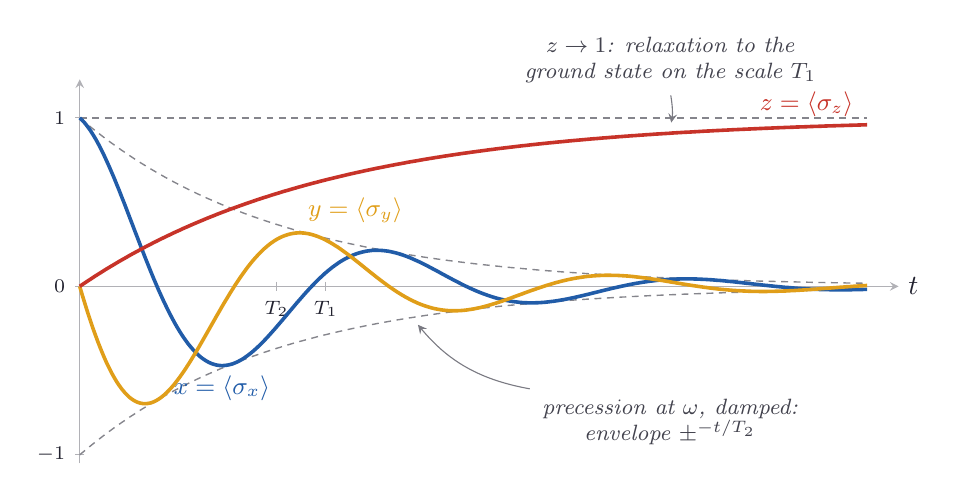
\begin{tikzpicture}[ink/.style={line width=0.9pt, ndInk}, faint/.style={line width=0.4pt, ndInk!35}, dashedink/.style={line width=0.5pt, ndInk!55, dash pattern=on 2.5pt off 2pt}, vec/.style={->, >=stealth, line width=1.2pt}, note/.style={font=\footnotesize\itshape, text=ndInk!85, align=center}, pointer/.style={->, >=stealth, line width=0.4pt, ndInk!60, shorten >=2pt, shorten <=1pt}, dot/.style={circle, fill=ndInk, inner sep=0pt, minimum size=3.4pt}, wash/.style={fill=ndSky, fill opacity=0.55}, every node/.style={text=ndInk}]
\definecolor{ndInk}{rgb}{0.13,0.13,0.18}
\definecolor{ndPaper}{rgb}{0.99,0.96,0.88}
\definecolor{ndSky}{rgb}{0.84,0.91,0.98}
\definecolor{ndRose}{rgb}{0.98,0.86,0.84}
\definecolor{ndBlue}{rgb}{0.13,0.36,0.66}
\definecolor{ndRed}{rgb}{0.78,0.20,0.16}
\definecolor{ndGold}{rgb}{0.88,0.62,0.10}
\definecolor{ndGreen}{rgb}{0.18,0.52,0.30}
\draw[faint, ->, >=stealth] (0.000,2.247) -- (10.400,2.247) node[right, text=ndInk] {$t$};
\draw[faint, ->, >=stealth] (0.000,0.000) -- (0.000,4.876) node[above, text=ndInk] {};
\draw[faint] (2.500,2.307) -- (2.500,2.187) node[below, font=\scriptsize, text=ndInk] {$T_2$};
\draw[faint] (3.125,2.307) -- (3.125,2.187) node[below, font=\scriptsize, text=ndInk] {$T_1$};
\draw[faint] (0.060,0.107) -- (-0.060,0.107) node[left, font=\scriptsize, text=ndInk] {$-1$};
\draw[faint] (0.060,2.247) -- (-0.060,2.247) node[left, font=\scriptsize, text=ndInk] {$0$};
\draw[faint] (0.060,4.386) -- (-0.060,4.386) node[left, font=\scriptsize, text=ndInk] {$1$};
\draw[dashedink] (0.000,4.386) -- (0.033,4.358) -- (0.067,4.330) -- (0.100,4.302) -- (0.134,4.275) -- (0.167,4.248) -- (0.201,4.221) -- (0.234,4.195) -- (0.268,4.169) -- (0.301,4.143) -- (0.334,4.118) -- (0.368,4.093) -- (0.401,4.069) -- (0.435,4.045) -- (0.468,4.021) -- (0.502,3.997) -- (0.535,3.974) -- (0.569,3.951) -- (0.602,3.928) -- (0.635,3.906) -- (0.669,3.884) -- (0.702,3.862) -- (0.736,3.841) -- (0.769,3.819) -- (0.803,3.798) -- (0.836,3.778) -- (0.870,3.757) -- (0.903,3.737) -- (0.936,3.718) -- (0.970,3.698) -- (1.003,3.679) -- (1.037,3.660) -- (1.070,3.641) -- (1.104,3.622) -- (1.137,3.604) -- (1.171,3.586) -- (1.204,3.568) -- (1.237,3.551) -- (1.271,3.533) -- (1.304,3.516) -- (1.338,3.499) -- (1.371,3.483) -- (1.405,3.466) -- (1.438,3.450) -- (1.472,3.434) -- (1.505,3.418) -- (1.538,3.403) -- (1.572,3.387) -- (1.605,3.372) -- (1.639,3.357) -- (1.672,3.343) -- (1.706,3.328) -- (1.739,3.314) -- (1.773,3.299) -- (1.806,3.285) -- (1.839,3.272) -- (1.873,3.258) -- (1.906,3.245) -- (1.940,3.231) -- (1.973,3.218) -- (2.007,3.205) -- (2.040,3.193) -- (2.074,3.180) -- (2.107,3.168) -- (2.140,3.155) -- (2.174,3.143) -- (2.207,3.131) -- (2.241,3.120) -- (2.274,3.108) -- (2.308,3.097) -- (2.341,3.085) -- (2.375,3.074) -- (2.408,3.063) -- (2.441,3.052) -- (2.475,3.042) -- (2.508,3.031) -- (2.542,3.021) -- (2.575,3.010) -- (2.609,3.000) -- (2.642,2.990) -- (2.676,2.980) -- (2.709,2.970) -- (2.742,2.961) -- (2.776,2.951) -- (2.809,2.942) -- (2.843,2.933) -- (2.876,2.924) -- (2.910,2.915) -- (2.943,2.906) -- (2.977,2.897) -- (3.010,2.888) -- (3.043,2.880) -- (3.077,2.871) -- (3.110,2.863) -- (3.144,2.855) -- (3.177,2.847) -- (3.211,2.839) -- (3.244,2.831) -- (3.278,2.823) -- (3.311,2.816) -- (3.344,2.808) -- (3.378,2.801) -- (3.411,2.793) -- (3.445,2.786) -- (3.478,2.779) -- (3.512,2.772) -- (3.545,2.765) -- (3.579,2.758) -- (3.612,2.751) -- (3.645,2.744) -- (3.679,2.738) -- (3.712,2.731) -- (3.746,2.725) -- (3.779,2.718) -- (3.813,2.712) -- (3.846,2.706) -- (3.880,2.700) -- (3.913,2.694) -- (3.946,2.688) -- (3.980,2.682) -- (4.013,2.676) -- (4.047,2.670) -- (4.080,2.665) -- (4.114,2.659) -- (4.147,2.654) -- (4.181,2.648) -- (4.214,2.643) -- (4.247,2.638) -- (4.281,2.633) -- (4.314,2.627) -- (4.348,2.622) -- (4.381,2.617) -- (4.415,2.612) -- (4.448,2.608) -- (4.482,2.603) -- (4.515,2.598) -- (4.548,2.593) -- (4.582,2.589) -- (4.615,2.584) -- (4.649,2.580) -- (4.682,2.575) -- (4.716,2.571) -- (4.749,2.567) -- (4.783,2.562) -- (4.816,2.558) -- (4.849,2.554) -- (4.883,2.550) -- (4.916,2.546) -- (4.950,2.542) -- (4.983,2.538) -- (5.017,2.534) -- (5.050,2.530) -- (5.084,2.527) -- (5.117,2.523) -- (5.151,2.519) -- (5.184,2.516) -- (5.217,2.512) -- (5.251,2.508) -- (5.284,2.505) -- (5.318,2.502) -- (5.351,2.498) -- (5.385,2.495) -- (5.418,2.491) -- (5.452,2.488) -- (5.485,2.485) -- (5.518,2.482) -- (5.552,2.479) -- (5.585,2.476) -- (5.619,2.473) -- (5.652,2.470) -- (5.686,2.467) -- (5.719,2.464) -- (5.753,2.461) -- (5.786,2.458) -- (5.819,2.455) -- (5.853,2.452) -- (5.886,2.450) -- (5.920,2.447) -- (5.953,2.444) -- (5.987,2.442) -- (6.020,2.439) -- (6.054,2.436) -- (6.087,2.434) -- (6.120,2.431) -- (6.154,2.429) -- (6.187,2.427) -- (6.221,2.424) -- (6.254,2.422) -- (6.288,2.420) -- (6.321,2.417) -- (6.355,2.415) -- (6.388,2.413) -- (6.421,2.410) -- (6.455,2.408) -- (6.488,2.406) -- (6.522,2.404) -- (6.555,2.402) -- (6.589,2.400) -- (6.622,2.398) -- (6.656,2.396) -- (6.689,2.394) -- (6.722,2.392) -- (6.756,2.390) -- (6.789,2.388) -- (6.823,2.386) -- (6.856,2.384) -- (6.890,2.382) -- (6.923,2.381) -- (6.957,2.379) -- (6.990,2.377) -- (7.023,2.375) -- (7.057,2.374) -- (7.090,2.372) -- (7.124,2.370) -- (7.157,2.369) -- (7.191,2.367) -- (7.224,2.365) -- (7.258,2.364) -- (7.291,2.362) -- (7.324,2.361) -- (7.358,2.359) -- (7.391,2.358) -- (7.425,2.356) -- (7.458,2.355) -- (7.492,2.353) -- (7.525,2.352) -- (7.559,2.351) -- (7.592,2.349) -- (7.625,2.348) -- (7.659,2.346) -- (7.692,2.345) -- (7.726,2.344) -- (7.759,2.343) -- (7.793,2.341) -- (7.826,2.340) -- (7.860,2.339) -- (7.893,2.338) -- (7.926,2.336) -- (7.960,2.335) -- (7.993,2.334) -- (8.027,2.333) -- (8.060,2.332) -- (8.094,2.331) -- (8.127,2.329) -- (8.161,2.328) -- (8.194,2.327) -- (8.227,2.326) -- (8.261,2.325) -- (8.294,2.324) -- (8.328,2.323) -- (8.361,2.322) -- (8.395,2.321) -- (8.428,2.320) -- (8.462,2.319) -- (8.495,2.318) -- (8.528,2.317) -- (8.562,2.316) -- (8.595,2.315) -- (8.629,2.314) -- (8.662,2.313) -- (8.696,2.313) -- (8.729,2.312) -- (8.763,2.311) -- (8.796,2.310) -- (8.829,2.309) -- (8.863,2.308) -- (8.896,2.307) -- (8.930,2.307) -- (8.963,2.306) -- (8.997,2.305) -- (9.030,2.304) -- (9.064,2.304) -- (9.097,2.303) -- (9.130,2.302) -- (9.164,2.301) -- (9.197,2.301) -- (9.231,2.300) -- (9.264,2.299) -- (9.298,2.298) -- (9.331,2.298) -- (9.365,2.297) -- (9.398,2.296) -- (9.431,2.296) -- (9.465,2.295) -- (9.498,2.294) -- (9.532,2.294) -- (9.565,2.293) -- (9.599,2.293) -- (9.632,2.292) -- (9.666,2.291) -- (9.699,2.291) -- (9.732,2.290) -- (9.766,2.290) -- (9.799,2.289) -- (9.833,2.288) -- (9.866,2.288) -- (9.900,2.287) -- (9.933,2.287) -- (9.967,2.286) -- (10.000,2.286);
\draw[dashedink] (0.000,0.107) -- (0.033,0.135) -- (0.067,0.163) -- (0.100,0.191) -- (0.134,0.218) -- (0.167,0.245) -- (0.201,0.272) -- (0.234,0.298) -- (0.268,0.324) -- (0.301,0.350) -- (0.334,0.375) -- (0.368,0.400) -- (0.401,0.424) -- (0.435,0.449) -- (0.468,0.472) -- (0.502,0.496) -- (0.535,0.519) -- (0.569,0.542) -- (0.602,0.565) -- (0.635,0.587) -- (0.669,0.609) -- (0.702,0.631) -- (0.736,0.652) -- (0.769,0.674) -- (0.803,0.695) -- (0.836,0.715) -- (0.870,0.736) -- (0.903,0.756) -- (0.936,0.775) -- (0.970,0.795) -- (1.003,0.814) -- (1.037,0.833) -- (1.070,0.852) -- (1.104,0.871) -- (1.137,0.889) -- (1.171,0.907) -- (1.204,0.925) -- (1.237,0.942) -- (1.271,0.960) -- (1.304,0.977) -- (1.338,0.994) -- (1.371,1.010) -- (1.405,1.027) -- (1.438,1.043) -- (1.472,1.059) -- (1.505,1.075) -- (1.538,1.090) -- (1.572,1.106) -- (1.605,1.121) -- (1.639,1.136) -- (1.672,1.150) -- (1.706,1.165) -- (1.739,1.179) -- (1.773,1.194) -- (1.806,1.208) -- (1.839,1.221) -- (1.873,1.235) -- (1.906,1.248) -- (1.940,1.262) -- (1.973,1.275) -- (2.007,1.288) -- (2.040,1.300) -- (2.074,1.313) -- (2.107,1.325) -- (2.140,1.338) -- (2.174,1.350) -- (2.207,1.362) -- (2.241,1.373) -- (2.274,1.385) -- (2.308,1.396) -- (2.341,1.408) -- (2.375,1.419) -- (2.408,1.430) -- (2.441,1.441) -- (2.475,1.451) -- (2.508,1.462) -- (2.542,1.472) -- (2.575,1.483) -- (2.609,1.493) -- (2.642,1.503) -- (2.676,1.513) -- (2.709,1.523) -- (2.742,1.532) -- (2.776,1.542) -- (2.809,1.551) -- (2.843,1.560) -- (2.876,1.569) -- (2.910,1.578) -- (2.943,1.587) -- (2.977,1.596) -- (3.010,1.605) -- (3.043,1.613) -- (3.077,1.622) -- (3.110,1.630) -- (3.144,1.638) -- (3.177,1.646) -- (3.211,1.654) -- (3.244,1.662) -- (3.278,1.670) -- (3.311,1.677) -- (3.344,1.685) -- (3.378,1.693) -- (3.411,1.700) -- (3.445,1.707) -- (3.478,1.714) -- (3.512,1.721) -- (3.545,1.728) -- (3.579,1.735) -- (3.612,1.742) -- (3.645,1.749) -- (3.679,1.755) -- (3.712,1.762) -- (3.746,1.768) -- (3.779,1.775) -- (3.813,1.781) -- (3.846,1.787) -- (3.880,1.793) -- (3.913,1.799) -- (3.946,1.805) -- (3.980,1.811) -- (4.013,1.817) -- (4.047,1.823) -- (4.080,1.828) -- (4.114,1.834) -- (4.147,1.839) -- (4.181,1.845) -- (4.214,1.850) -- (4.247,1.855) -- (4.281,1.860) -- (4.314,1.866) -- (4.348,1.871) -- (4.381,1.876) -- (4.415,1.881) -- (4.448,1.885) -- (4.482,1.890) -- (4.515,1.895) -- (4.548,1.900) -- (4.582,1.904) -- (4.615,1.909) -- (4.649,1.913) -- (4.682,1.918) -- (4.716,1.922) -- (4.749,1.926) -- (4.783,1.931) -- (4.816,1.935) -- (4.849,1.939) -- (4.883,1.943) -- (4.916,1.947) -- (4.950,1.951) -- (4.983,1.955) -- (5.017,1.959) -- (5.050,1.963) -- (5.084,1.966) -- (5.117,1.970) -- (5.151,1.974) -- (5.184,1.977) -- (5.217,1.981) -- (5.251,1.985) -- (5.284,1.988) -- (5.318,1.992) -- (5.351,1.995) -- (5.385,1.998) -- (5.418,2.002) -- (5.452,2.005) -- (5.485,2.008) -- (5.518,2.011) -- (5.552,2.014) -- (5.585,2.017) -- (5.619,2.020) -- (5.652,2.023) -- (5.686,2.026) -- (5.719,2.029) -- (5.753,2.032) -- (5.786,2.035) -- (5.819,2.038) -- (5.853,2.041) -- (5.886,2.043) -- (5.920,2.046) -- (5.953,2.049) -- (5.987,2.051) -- (6.020,2.054) -- (6.054,2.057) -- (6.087,2.059) -- (6.120,2.062) -- (6.154,2.064) -- (6.187,2.066) -- (6.221,2.069) -- (6.254,2.071) -- (6.288,2.074) -- (6.321,2.076) -- (6.355,2.078) -- (6.388,2.080) -- (6.421,2.083) -- (6.455,2.085) -- (6.488,2.087) -- (6.522,2.089) -- (6.555,2.091) -- (6.589,2.093) -- (6.622,2.095) -- (6.656,2.097) -- (6.689,2.099) -- (6.722,2.101) -- (6.756,2.103) -- (6.789,2.105) -- (6.823,2.107) -- (6.856,2.109) -- (6.890,2.111) -- (6.923,2.112) -- (6.957,2.114) -- (6.990,2.116) -- (7.023,2.118) -- (7.057,2.119) -- (7.090,2.121) -- (7.124,2.123) -- (7.157,2.124) -- (7.191,2.126) -- (7.224,2.128) -- (7.258,2.129) -- (7.291,2.131) -- (7.324,2.132) -- (7.358,2.134) -- (7.391,2.135) -- (7.425,2.137) -- (7.458,2.138) -- (7.492,2.140) -- (7.525,2.141) -- (7.559,2.142) -- (7.592,2.144) -- (7.625,2.145) -- (7.659,2.147) -- (7.692,2.148) -- (7.726,2.149) -- (7.759,2.150) -- (7.793,2.152) -- (7.826,2.153) -- (7.860,2.154) -- (7.893,2.155) -- (7.926,2.157) -- (7.960,2.158) -- (7.993,2.159) -- (8.027,2.160) -- (8.060,2.161) -- (8.094,2.163) -- (8.127,2.164) -- (8.161,2.165) -- (8.194,2.166) -- (8.227,2.167) -- (8.261,2.168) -- (8.294,2.169) -- (8.328,2.170) -- (8.361,2.171) -- (8.395,2.172) -- (8.428,2.173) -- (8.462,2.174) -- (8.495,2.175) -- (8.528,2.176) -- (8.562,2.177) -- (8.595,2.178) -- (8.629,2.179) -- (8.662,2.180) -- (8.696,2.180) -- (8.729,2.181) -- (8.763,2.182) -- (8.796,2.183) -- (8.829,2.184) -- (8.863,2.185) -- (8.896,2.186) -- (8.930,2.186) -- (8.963,2.187) -- (8.997,2.188) -- (9.030,2.189) -- (9.064,2.190) -- (9.097,2.190) -- (9.130,2.191) -- (9.164,2.192) -- (9.197,2.192) -- (9.231,2.193) -- (9.264,2.194) -- (9.298,2.195) -- (9.331,2.195) -- (9.365,2.196) -- (9.398,2.197) -- (9.431,2.197) -- (9.465,2.198) -- (9.498,2.199) -- (9.532,2.199) -- (9.565,2.200) -- (9.599,2.201) -- (9.632,2.201) -- (9.666,2.202) -- (9.699,2.202) -- (9.732,2.203) -- (9.766,2.203) -- (9.799,2.204) -- (9.833,2.205) -- (9.866,2.205) -- (9.900,2.206) -- (9.933,2.206) -- (9.967,2.207) -- (10.000,2.207);
\draw[dashedink] (0.000,4.386) -- (10.000,4.386);
\draw[line width=1.3pt, ndBlue] (0.000,4.386) -- (0.033,4.355) -- (0.067,4.318) -- (0.100,4.275) -- (0.134,4.228) -- (0.167,4.176) -- (0.201,4.120) -- (0.234,4.060) -- (0.268,3.995) -- (0.301,3.928) -- (0.334,3.857) -- (0.368,3.782) -- (0.401,3.706) -- (0.435,3.627) -- (0.468,3.546) -- (0.502,3.463) -- (0.535,3.378) -- (0.569,3.293) -- (0.602,3.207) -- (0.635,3.120) -- (0.669,3.032) -- (0.702,2.945) -- (0.736,2.858) -- (0.769,2.771) -- (0.803,2.685) -- (0.836,2.600) -- (0.870,2.516) -- (0.903,2.434) -- (0.936,2.353) -- (0.970,2.274) -- (1.003,2.197) -- (1.037,2.122) -- (1.070,2.050) -- (1.104,1.980) -- (1.137,1.912) -- (1.171,1.848) -- (1.204,1.786) -- (1.237,1.728) -- (1.271,1.672) -- (1.304,1.620) -- (1.338,1.571) -- (1.371,1.525) -- (1.405,1.483) -- (1.438,1.444) -- (1.472,1.408) -- (1.505,1.376) -- (1.538,1.347) -- (1.572,1.322) -- (1.605,1.301) -- (1.639,1.282) -- (1.672,1.267) -- (1.706,1.256) -- (1.739,1.247) -- (1.773,1.242) -- (1.806,1.240) -- (1.839,1.242) -- (1.873,1.246) -- (1.906,1.253) -- (1.940,1.262) -- (1.973,1.275) -- (2.007,1.290) -- (2.040,1.308) -- (2.074,1.327) -- (2.107,1.350) -- (2.140,1.374) -- (2.174,1.400) -- (2.207,1.428) -- (2.241,1.458) -- (2.274,1.489) -- (2.308,1.522) -- (2.341,1.556) -- (2.375,1.592) -- (2.408,1.628) -- (2.441,1.665) -- (2.475,1.703) -- (2.508,1.742) -- (2.542,1.781) -- (2.575,1.820) -- (2.609,1.860) -- (2.642,1.900) -- (2.676,1.940) -- (2.709,1.979) -- (2.742,2.019) -- (2.776,2.058) -- (2.809,2.096) -- (2.843,2.135) -- (2.876,2.172) -- (2.910,2.209) -- (2.943,2.244) -- (2.977,2.279) -- (3.010,2.313) -- (3.043,2.346) -- (3.077,2.377) -- (3.110,2.408) -- (3.144,2.437) -- (3.177,2.464) -- (3.211,2.491) -- (3.244,2.515) -- (3.278,2.539) -- (3.311,2.561) -- (3.344,2.581) -- (3.378,2.600) -- (3.411,2.617) -- (3.445,2.633) -- (3.478,2.647) -- (3.512,2.660) -- (3.545,2.671) -- (3.579,2.680) -- (3.612,2.688) -- (3.645,2.695) -- (3.679,2.699) -- (3.712,2.703) -- (3.746,2.705) -- (3.779,2.705) -- (3.813,2.704) -- (3.846,2.702) -- (3.880,2.698) -- (3.913,2.694) -- (3.946,2.688) -- (3.980,2.680) -- (4.013,2.672) -- (4.047,2.663) -- (4.080,2.652) -- (4.114,2.641) -- (4.147,2.629) -- (4.181,2.616) -- (4.214,2.602) -- (4.247,2.587) -- (4.281,2.572) -- (4.314,2.557) -- (4.348,2.540) -- (4.381,2.524) -- (4.415,2.507) -- (4.448,2.489) -- (4.482,2.471) -- (4.515,2.454) -- (4.548,2.436) -- (4.582,2.417) -- (4.615,2.399) -- (4.649,2.381) -- (4.682,2.363) -- (4.716,2.345) -- (4.749,2.327) -- (4.783,2.310) -- (4.816,2.293) -- (4.849,2.276) -- (4.883,2.259) -- (4.916,2.243) -- (4.950,2.227) -- (4.983,2.212) -- (5.017,2.197) -- (5.050,2.183) -- (5.084,2.169) -- (5.117,2.156) -- (5.151,2.144) -- (5.184,2.132) -- (5.217,2.121) -- (5.251,2.110) -- (5.284,2.100) -- (5.318,2.091) -- (5.351,2.083) -- (5.385,2.075) -- (5.418,2.068) -- (5.452,2.062) -- (5.485,2.056) -- (5.518,2.052) -- (5.552,2.048) -- (5.585,2.044) -- (5.619,2.041) -- (5.652,2.039) -- (5.686,2.038) -- (5.719,2.037) -- (5.753,2.037) -- (5.786,2.038) -- (5.819,2.039) -- (5.853,2.041) -- (5.886,2.043) -- (5.920,2.046) -- (5.953,2.050) -- (5.987,2.054) -- (6.020,2.058) -- (6.054,2.063) -- (6.087,2.068) -- (6.120,2.074) -- (6.154,2.080) -- (6.187,2.086) -- (6.221,2.093) -- (6.254,2.100) -- (6.288,2.107) -- (6.321,2.115) -- (6.355,2.122) -- (6.388,2.130) -- (6.421,2.138) -- (6.455,2.146) -- (6.488,2.154) -- (6.522,2.163) -- (6.555,2.171) -- (6.589,2.179) -- (6.622,2.188) -- (6.656,2.196) -- (6.689,2.204) -- (6.722,2.212) -- (6.756,2.220) -- (6.789,2.228) -- (6.823,2.235) -- (6.856,2.243) -- (6.890,2.250) -- (6.923,2.257) -- (6.957,2.264) -- (6.990,2.271) -- (7.023,2.277) -- (7.057,2.284) -- (7.090,2.289) -- (7.124,2.295) -- (7.157,2.300) -- (7.191,2.305) -- (7.224,2.310) -- (7.258,2.314) -- (7.291,2.318) -- (7.324,2.322) -- (7.358,2.326) -- (7.391,2.329) -- (7.425,2.331) -- (7.458,2.334) -- (7.492,2.336) -- (7.525,2.338) -- (7.559,2.339) -- (7.592,2.340) -- (7.625,2.341) -- (7.659,2.342) -- (7.692,2.342) -- (7.726,2.342) -- (7.759,2.341) -- (7.793,2.341) -- (7.826,2.340) -- (7.860,2.339) -- (7.893,2.337) -- (7.926,2.336) -- (7.960,2.334) -- (7.993,2.332) -- (8.027,2.330) -- (8.060,2.327) -- (8.094,2.324) -- (8.127,2.322) -- (8.161,2.319) -- (8.194,2.316) -- (8.227,2.312) -- (8.261,2.309) -- (8.294,2.306) -- (8.328,2.302) -- (8.361,2.298) -- (8.395,2.295) -- (8.428,2.291) -- (8.462,2.287) -- (8.495,2.284) -- (8.528,2.280) -- (8.562,2.276) -- (8.595,2.272) -- (8.629,2.269) -- (8.662,2.265) -- (8.696,2.261) -- (8.729,2.258) -- (8.763,2.254) -- (8.796,2.251) -- (8.829,2.247) -- (8.863,2.244) -- (8.896,2.241) -- (8.930,2.237) -- (8.963,2.234) -- (8.997,2.232) -- (9.030,2.229) -- (9.064,2.226) -- (9.097,2.224) -- (9.130,2.221) -- (9.164,2.219) -- (9.197,2.217) -- (9.231,2.215) -- (9.264,2.213) -- (9.298,2.212) -- (9.331,2.210) -- (9.365,2.209) -- (9.398,2.207) -- (9.431,2.206) -- (9.465,2.205) -- (9.498,2.205) -- (9.532,2.204) -- (9.565,2.204) -- (9.599,2.203) -- (9.632,2.203) -- (9.666,2.203) -- (9.699,2.203) -- (9.732,2.203) -- (9.766,2.204) -- (9.799,2.204) -- (9.833,2.205) -- (9.866,2.205) -- (9.900,2.206) -- (9.933,2.207) -- (9.967,2.208) -- (10.000,2.209);
\node[font=\small, text=ndBlue, below] at (1.806,1.240) {$x=\langle\sigma_x\rangle$};
\draw[line width=1.3pt, ndGold] (0.000,2.247) -- (0.033,2.134) -- (0.067,2.024) -- (0.100,1.918) -- (0.134,1.816) -- (0.167,1.717) -- (0.201,1.623) -- (0.234,1.534) -- (0.268,1.448) -- (0.301,1.368) -- (0.334,1.292) -- (0.368,1.221) -- (0.401,1.155) -- (0.435,1.094) -- (0.468,1.038) -- (0.502,0.987) -- (0.535,0.942) -- (0.569,0.901) -- (0.602,0.866) -- (0.635,0.835) -- (0.669,0.810) -- (0.702,0.790) -- (0.736,0.774) -- (0.769,0.764) -- (0.803,0.758) -- (0.836,0.757) -- (0.870,0.760) -- (0.903,0.767) -- (0.936,0.779) -- (0.970,0.795) -- (1.003,0.815) -- (1.037,0.839) -- (1.070,0.866) -- (1.104,0.897) -- (1.137,0.931) -- (1.171,0.968) -- (1.204,1.007) -- (1.237,1.050) -- (1.271,1.095) -- (1.304,1.142) -- (1.338,1.191) -- (1.371,1.243) -- (1.405,1.295) -- (1.438,1.350) -- (1.472,1.405) -- (1.505,1.462) -- (1.538,1.519) -- (1.572,1.578) -- (1.605,1.636) -- (1.639,1.695) -- (1.672,1.754) -- (1.706,1.813) -- (1.739,1.872) -- (1.773,1.930) -- (1.806,1.988) -- (1.839,2.044) -- (1.873,2.100) -- (1.906,2.155) -- (1.940,2.209) -- (1.973,2.262) -- (2.007,2.313) -- (2.040,2.362) -- (2.074,2.410) -- (2.107,2.456) -- (2.140,2.500) -- (2.174,2.543) -- (2.207,2.583) -- (2.241,2.621) -- (2.274,2.657) -- (2.308,2.691) -- (2.341,2.723) -- (2.375,2.752) -- (2.408,2.780) -- (2.441,2.804) -- (2.475,2.827) -- (2.508,2.847) -- (2.542,2.865) -- (2.575,2.880) -- (2.609,2.893) -- (2.642,2.904) -- (2.676,2.913) -- (2.709,2.919) -- (2.742,2.924) -- (2.776,2.926) -- (2.809,2.926) -- (2.843,2.924) -- (2.876,2.920) -- (2.910,2.914) -- (2.943,2.906) -- (2.977,2.896) -- (3.010,2.885) -- (3.043,2.872) -- (3.077,2.858) -- (3.110,2.842) -- (3.144,2.824) -- (3.177,2.806) -- (3.211,2.786) -- (3.244,2.765) -- (3.278,2.744) -- (3.311,2.721) -- (3.344,2.697) -- (3.378,2.673) -- (3.411,2.648) -- (3.445,2.623) -- (3.478,2.597) -- (3.512,2.570) -- (3.545,2.544) -- (3.579,2.517) -- (3.612,2.490) -- (3.645,2.463) -- (3.679,2.436) -- (3.712,2.410) -- (3.746,2.383) -- (3.779,2.357) -- (3.813,2.331) -- (3.846,2.306) -- (3.880,2.281) -- (3.913,2.256) -- (3.946,2.233) -- (3.980,2.210) -- (4.013,2.187) -- (4.047,2.166) -- (4.080,2.145) -- (4.114,2.125) -- (4.147,2.106) -- (4.181,2.088) -- (4.214,2.071) -- (4.247,2.055) -- (4.281,2.039) -- (4.314,2.025) -- (4.348,2.012) -- (4.381,2.000) -- (4.415,1.989) -- (4.448,1.979) -- (4.482,1.970) -- (4.515,1.962) -- (4.548,1.956) -- (4.582,1.950) -- (4.615,1.945) -- (4.649,1.942) -- (4.682,1.939) -- (4.716,1.937) -- (4.749,1.937) -- (4.783,1.937) -- (4.816,1.938) -- (4.849,1.940) -- (4.883,1.943) -- (4.916,1.947) -- (4.950,1.952) -- (4.983,1.957) -- (5.017,1.963) -- (5.050,1.970) -- (5.084,1.977) -- (5.117,1.985) -- (5.151,1.994) -- (5.184,2.003) -- (5.217,2.013) -- (5.251,2.023) -- (5.284,2.033) -- (5.318,2.044) -- (5.351,2.055) -- (5.385,2.067) -- (5.418,2.078) -- (5.452,2.090) -- (5.485,2.102) -- (5.518,2.115) -- (5.552,2.127) -- (5.585,2.139) -- (5.619,2.151) -- (5.652,2.164) -- (5.686,2.176) -- (5.719,2.188) -- (5.753,2.200) -- (5.786,2.211) -- (5.819,2.223) -- (5.853,2.234) -- (5.886,2.245) -- (5.920,2.256) -- (5.953,2.266) -- (5.987,2.276) -- (6.020,2.286) -- (6.054,2.296) -- (6.087,2.304) -- (6.120,2.313) -- (6.154,2.321) -- (6.187,2.329) -- (6.221,2.336) -- (6.254,2.343) -- (6.288,2.349) -- (6.321,2.355) -- (6.355,2.360) -- (6.388,2.365) -- (6.421,2.370) -- (6.455,2.374) -- (6.488,2.377) -- (6.522,2.380) -- (6.555,2.382) -- (6.589,2.384) -- (6.622,2.386) -- (6.656,2.387) -- (6.689,2.388) -- (6.722,2.388) -- (6.756,2.387) -- (6.789,2.387) -- (6.823,2.386) -- (6.856,2.384) -- (6.890,2.382) -- (6.923,2.380) -- (6.957,2.378) -- (6.990,2.375) -- (7.023,2.372) -- (7.057,2.368) -- (7.090,2.364) -- (7.124,2.360) -- (7.157,2.356) -- (7.191,2.352) -- (7.224,2.347) -- (7.258,2.342) -- (7.291,2.337) -- (7.324,2.332) -- (7.358,2.327) -- (7.391,2.322) -- (7.425,2.316) -- (7.458,2.311) -- (7.492,2.305) -- (7.525,2.299) -- (7.559,2.294) -- (7.592,2.288) -- (7.625,2.283) -- (7.659,2.277) -- (7.692,2.272) -- (7.726,2.266) -- (7.759,2.261) -- (7.793,2.256) -- (7.826,2.251) -- (7.860,2.246) -- (7.893,2.241) -- (7.926,2.236) -- (7.960,2.232) -- (7.993,2.227) -- (8.027,2.223) -- (8.060,2.219) -- (8.094,2.215) -- (8.127,2.211) -- (8.161,2.208) -- (8.194,2.205) -- (8.227,2.202) -- (8.261,2.199) -- (8.294,2.196) -- (8.328,2.194) -- (8.361,2.192) -- (8.395,2.190) -- (8.428,2.188) -- (8.462,2.187) -- (8.495,2.185) -- (8.528,2.184) -- (8.562,2.183) -- (8.595,2.183) -- (8.629,2.182) -- (8.662,2.182) -- (8.696,2.182) -- (8.729,2.182) -- (8.763,2.183) -- (8.796,2.183) -- (8.829,2.184) -- (8.863,2.185) -- (8.896,2.186) -- (8.930,2.187) -- (8.963,2.188) -- (8.997,2.190) -- (9.030,2.192) -- (9.064,2.193) -- (9.097,2.195) -- (9.130,2.197) -- (9.164,2.199) -- (9.197,2.201) -- (9.231,2.204) -- (9.264,2.206) -- (9.298,2.208) -- (9.331,2.211) -- (9.365,2.213) -- (9.398,2.216) -- (9.431,2.218) -- (9.465,2.221) -- (9.498,2.223) -- (9.532,2.226) -- (9.565,2.228) -- (9.599,2.231) -- (9.632,2.233) -- (9.666,2.236) -- (9.699,2.238) -- (9.732,2.241) -- (9.766,2.243) -- (9.799,2.245) -- (9.833,2.248) -- (9.866,2.250) -- (9.900,2.252) -- (9.933,2.254) -- (9.967,2.256) -- (10.000,2.258);
\node[font=\small, text=ndGold, above right] at (2.776,2.926) {$y=\langle\sigma_y\rangle$};
\draw[line width=1.3pt, ndRed] (0.000,2.247) -- (0.033,2.269) -- (0.067,2.292) -- (0.100,2.314) -- (0.134,2.336) -- (0.167,2.358) -- (0.201,2.380) -- (0.234,2.401) -- (0.268,2.422) -- (0.301,2.443) -- (0.334,2.464) -- (0.368,2.484) -- (0.401,2.504) -- (0.435,2.524) -- (0.468,2.544) -- (0.502,2.564) -- (0.535,2.583) -- (0.569,2.602) -- (0.602,2.621) -- (0.635,2.640) -- (0.669,2.659) -- (0.702,2.677) -- (0.736,2.695) -- (0.769,2.713) -- (0.803,2.731) -- (0.836,2.749) -- (0.870,2.766) -- (0.903,2.783) -- (0.936,2.801) -- (0.970,2.817) -- (1.003,2.834) -- (1.037,2.851) -- (1.070,2.867) -- (1.104,2.883) -- (1.137,2.899) -- (1.171,2.915) -- (1.204,2.931) -- (1.237,2.946) -- (1.271,2.961) -- (1.304,2.977) -- (1.338,2.992) -- (1.371,3.006) -- (1.405,3.021) -- (1.438,3.036) -- (1.472,3.050) -- (1.505,3.064) -- (1.538,3.078) -- (1.572,3.092) -- (1.605,3.106) -- (1.639,3.120) -- (1.672,3.133) -- (1.706,3.146) -- (1.739,3.160) -- (1.773,3.173) -- (1.806,3.186) -- (1.839,3.198) -- (1.873,3.211) -- (1.906,3.224) -- (1.940,3.236) -- (1.973,3.248) -- (2.007,3.260) -- (2.040,3.272) -- (2.074,3.284) -- (2.107,3.296) -- (2.140,3.307) -- (2.174,3.319) -- (2.207,3.330) -- (2.241,3.342) -- (2.274,3.353) -- (2.308,3.364) -- (2.341,3.375) -- (2.375,3.385) -- (2.408,3.396) -- (2.441,3.407) -- (2.475,3.417) -- (2.508,3.427) -- (2.542,3.437) -- (2.575,3.448) -- (2.609,3.458) -- (2.642,3.467) -- (2.676,3.477) -- (2.709,3.487) -- (2.742,3.496) -- (2.776,3.506) -- (2.809,3.515) -- (2.843,3.525) -- (2.876,3.534) -- (2.910,3.543) -- (2.943,3.552) -- (2.977,3.561) -- (3.010,3.569) -- (3.043,3.578) -- (3.077,3.587) -- (3.110,3.595) -- (3.144,3.604) -- (3.177,3.612) -- (3.211,3.620) -- (3.244,3.628) -- (3.278,3.636) -- (3.311,3.644) -- (3.344,3.652) -- (3.378,3.660) -- (3.411,3.668) -- (3.445,3.676) -- (3.478,3.683) -- (3.512,3.691) -- (3.545,3.698) -- (3.579,3.705) -- (3.612,3.713) -- (3.645,3.720) -- (3.679,3.727) -- (3.712,3.734) -- (3.746,3.741) -- (3.779,3.748) -- (3.813,3.754) -- (3.846,3.761) -- (3.880,3.768) -- (3.913,3.774) -- (3.946,3.781) -- (3.980,3.787) -- (4.013,3.794) -- (4.047,3.800) -- (4.080,3.806) -- (4.114,3.812) -- (4.147,3.819) -- (4.181,3.825) -- (4.214,3.831) -- (4.247,3.836) -- (4.281,3.842) -- (4.314,3.848) -- (4.348,3.854) -- (4.381,3.860) -- (4.415,3.865) -- (4.448,3.871) -- (4.482,3.876) -- (4.515,3.882) -- (4.548,3.887) -- (4.582,3.892) -- (4.615,3.898) -- (4.649,3.903) -- (4.682,3.908) -- (4.716,3.913) -- (4.749,3.918) -- (4.783,3.923) -- (4.816,3.928) -- (4.849,3.933) -- (4.883,3.938) -- (4.916,3.942) -- (4.950,3.947) -- (4.983,3.952) -- (5.017,3.956) -- (5.050,3.961) -- (5.084,3.965) -- (5.117,3.970) -- (5.151,3.974) -- (5.184,3.979) -- (5.217,3.983) -- (5.251,3.987) -- (5.284,3.992) -- (5.318,3.996) -- (5.351,4.000) -- (5.385,4.004) -- (5.418,4.008) -- (5.452,4.012) -- (5.485,4.016) -- (5.518,4.020) -- (5.552,4.024) -- (5.585,4.028) -- (5.619,4.032) -- (5.652,4.035) -- (5.686,4.039) -- (5.719,4.043) -- (5.753,4.047) -- (5.786,4.050) -- (5.819,4.054) -- (5.853,4.057) -- (5.886,4.061) -- (5.920,4.064) -- (5.953,4.068) -- (5.987,4.071) -- (6.020,4.074) -- (6.054,4.078) -- (6.087,4.081) -- (6.120,4.084) -- (6.154,4.087) -- (6.187,4.091) -- (6.221,4.094) -- (6.254,4.097) -- (6.288,4.100) -- (6.321,4.103) -- (6.355,4.106) -- (6.388,4.109) -- (6.421,4.112) -- (6.455,4.115) -- (6.488,4.118) -- (6.522,4.121) -- (6.555,4.123) -- (6.589,4.126) -- (6.622,4.129) -- (6.656,4.132) -- (6.689,4.134) -- (6.722,4.137) -- (6.756,4.140) -- (6.789,4.142) -- (6.823,4.145) -- (6.856,4.148) -- (6.890,4.150) -- (6.923,4.153) -- (6.957,4.155) -- (6.990,4.158) -- (7.023,4.160) -- (7.057,4.162) -- (7.090,4.165) -- (7.124,4.167) -- (7.157,4.169) -- (7.191,4.172) -- (7.224,4.174) -- (7.258,4.176) -- (7.291,4.179) -- (7.324,4.181) -- (7.358,4.183) -- (7.391,4.185) -- (7.425,4.187) -- (7.458,4.189) -- (7.492,4.191) -- (7.525,4.194) -- (7.559,4.196) -- (7.592,4.198) -- (7.625,4.200) -- (7.659,4.202) -- (7.692,4.204) -- (7.726,4.205) -- (7.759,4.207) -- (7.793,4.209) -- (7.826,4.211) -- (7.860,4.213) -- (7.893,4.215) -- (7.926,4.217) -- (7.960,4.219) -- (7.993,4.220) -- (8.027,4.222) -- (8.060,4.224) -- (8.094,4.226) -- (8.127,4.227) -- (8.161,4.229) -- (8.194,4.231) -- (8.227,4.232) -- (8.261,4.234) -- (8.294,4.236) -- (8.328,4.237) -- (8.361,4.239) -- (8.395,4.240) -- (8.428,4.242) -- (8.462,4.243) -- (8.495,4.245) -- (8.528,4.246) -- (8.562,4.248) -- (8.595,4.249) -- (8.629,4.251) -- (8.662,4.252) -- (8.696,4.254) -- (8.729,4.255) -- (8.763,4.256) -- (8.796,4.258) -- (8.829,4.259) -- (8.863,4.261) -- (8.896,4.262) -- (8.930,4.263) -- (8.963,4.265) -- (8.997,4.266) -- (9.030,4.267) -- (9.064,4.268) -- (9.097,4.270) -- (9.130,4.271) -- (9.164,4.272) -- (9.197,4.273) -- (9.231,4.274) -- (9.264,4.276) -- (9.298,4.277) -- (9.331,4.278) -- (9.365,4.279) -- (9.398,4.280) -- (9.431,4.281) -- (9.465,4.283) -- (9.498,4.284) -- (9.532,4.285) -- (9.565,4.286) -- (9.599,4.287) -- (9.632,4.288) -- (9.666,4.289) -- (9.699,4.290) -- (9.732,4.291) -- (9.766,4.292) -- (9.799,4.293) -- (9.833,4.294) -- (9.866,4.295) -- (9.900,4.296) -- (9.933,4.297) -- (9.967,4.298) -- (10.000,4.299);
\node[font=\small, text=ndRed, above] at (9.231,4.274) {$z=\langle\sigma_z\rangle$};
\node[note, anchor=south west] (e) at (5.750,0.107) {precession at $\omega$, damped:\\ envelope $\pm\ee^{-t/T_2}$};
\draw[pointer] (e.north west) to[bend left=20] (4.250,1.813);
\node[note, anchor=south] (z) at (7.500,4.707) {$z\to1$: relaxation to the\\ ground state on the scale $T_1$};
\draw[pointer] (z.south) to[bend left=10] (7.500,4.258);
\end{tikzpicture}
}
\caption{Bloch components of a qubit with $\omega=2$, $\gamma_1=0.4$, $\gamma_\phi=0.3$ (so $T_1=2.5$, $T_2=2$), starting in $\ket+$: the precession of $x,y$ is damped inside the envelopes $\pm\ee^{-t/T_2}$ (dashed), and $z$ relaxes to the ground state $z=1$ as $1-\ee^{-t/T_1}$. Generated by \texttt{code/ch03\_decoherence.py}.}\label{fig:ch03:decoherence}
\end{figure}}
\ona{\endgraf\medskip\noindent\textit{Reading the figure.} The three curves are the averages $\langle\sigx\rangle$, $\langle\sigy\rangle$, $\langle\sigz\rangle$ that one would measure at time $t$, starting from $\ket+$, which points along the $x$-axis of the Bloch sphere. The curves $x$ and $y$ oscillate because the qubit precesses about the $z$-axis at frequency $\omega$, like the hand of a clock, and the oscillation shrinks inside the dashed envelope $\pm\ee^{-t/T_2}$: the qubit forgets its phase. The curve $z$ climbs to $1$: the qubit loses its energy and settles in the ground state on the timescale $T_1$.\endgraf\smallskip\noindent\textit{Why it matters.} $T_1$ and $T_2$ are the two numbers quoted on every datasheet of quantum hardware (\Chap~\ref{C.Motivation}). $T_2$ bounds how long a superposition, the resource that distinguishes a qubit from a bit, survives; $T_1$ bounds how long an excited state survives; and always $T_2\le2T_1$, because $1/T_2=1/(2T_1)+\gamma_\phi$. A computer scientist may think of them as the retention time of a memory cell that leaks: every computation must finish, or be protected by error correction, well within these times.}
\onp{\begin{itemize}\item system matrix not antisymmetric: purity decreases; \item affine term: fixed point $z=1$ (ground state) rather than the origin.\end{itemize}}
\end{frame}

\begin{frame}<presentation>\ft{Relaxation and dephasing, pictured}
\begin{center}\resizebox{\linewidth}{!}{% Generated by code/needham.py -- do not edit by hand.
\definecolor{qocA}{rgb}{0.00,0.45,0.70}
\definecolor{qocB}{rgb}{0.90,0.60,0.00}
\definecolor{qocC}{rgb}{0.00,0.62,0.45}
\definecolor{qocD}{rgb}{0.80,0.40,0.00}
\definecolor{qocE}{rgb}{0.80,0.60,0.70}
\definecolor{qocF}{rgb}{0.35,0.70,0.90}
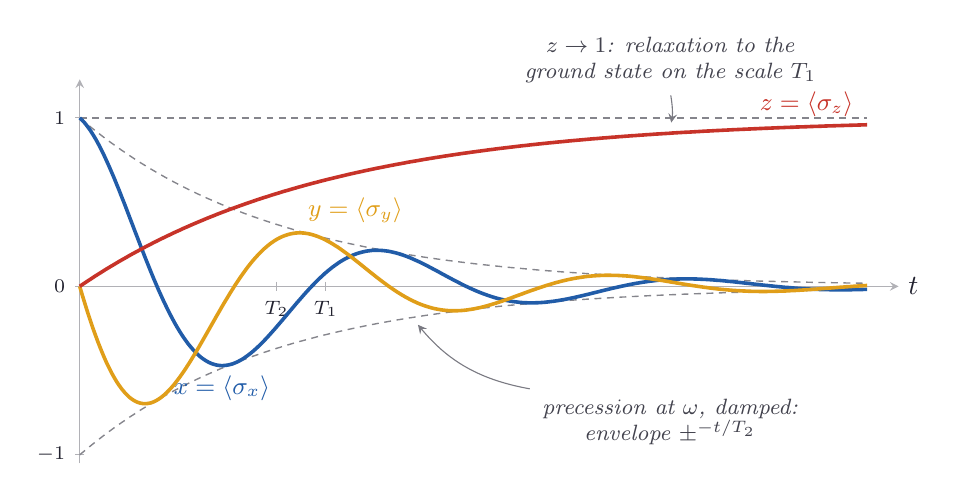
\begin{tikzpicture}[ink/.style={line width=0.9pt, ndInk}, faint/.style={line width=0.4pt, ndInk!35}, dashedink/.style={line width=0.5pt, ndInk!55, dash pattern=on 2.5pt off 2pt}, vec/.style={->, >=stealth, line width=1.2pt}, note/.style={font=\footnotesize\itshape, text=ndInk!85, align=center}, pointer/.style={->, >=stealth, line width=0.4pt, ndInk!60, shorten >=2pt, shorten <=1pt}, dot/.style={circle, fill=ndInk, inner sep=0pt, minimum size=3.4pt}, wash/.style={fill=ndSky, fill opacity=0.55}, every node/.style={text=ndInk}]
\definecolor{ndInk}{rgb}{0.13,0.13,0.18}
\definecolor{ndPaper}{rgb}{0.99,0.96,0.88}
\definecolor{ndSky}{rgb}{0.84,0.91,0.98}
\definecolor{ndRose}{rgb}{0.98,0.86,0.84}
\definecolor{ndBlue}{rgb}{0.13,0.36,0.66}
\definecolor{ndRed}{rgb}{0.78,0.20,0.16}
\definecolor{ndGold}{rgb}{0.88,0.62,0.10}
\definecolor{ndGreen}{rgb}{0.18,0.52,0.30}
\draw[faint, ->, >=stealth] (0.000,2.247) -- (10.400,2.247) node[right, text=ndInk] {$t$};
\draw[faint, ->, >=stealth] (0.000,0.000) -- (0.000,4.876) node[above, text=ndInk] {};
\draw[faint] (2.500,2.307) -- (2.500,2.187) node[below, font=\scriptsize, text=ndInk] {$T_2$};
\draw[faint] (3.125,2.307) -- (3.125,2.187) node[below, font=\scriptsize, text=ndInk] {$T_1$};
\draw[faint] (0.060,0.107) -- (-0.060,0.107) node[left, font=\scriptsize, text=ndInk] {$-1$};
\draw[faint] (0.060,2.247) -- (-0.060,2.247) node[left, font=\scriptsize, text=ndInk] {$0$};
\draw[faint] (0.060,4.386) -- (-0.060,4.386) node[left, font=\scriptsize, text=ndInk] {$1$};
\draw[dashedink] (0.000,4.386) -- (0.033,4.358) -- (0.067,4.330) -- (0.100,4.302) -- (0.134,4.275) -- (0.167,4.248) -- (0.201,4.221) -- (0.234,4.195) -- (0.268,4.169) -- (0.301,4.143) -- (0.334,4.118) -- (0.368,4.093) -- (0.401,4.069) -- (0.435,4.045) -- (0.468,4.021) -- (0.502,3.997) -- (0.535,3.974) -- (0.569,3.951) -- (0.602,3.928) -- (0.635,3.906) -- (0.669,3.884) -- (0.702,3.862) -- (0.736,3.841) -- (0.769,3.819) -- (0.803,3.798) -- (0.836,3.778) -- (0.870,3.757) -- (0.903,3.737) -- (0.936,3.718) -- (0.970,3.698) -- (1.003,3.679) -- (1.037,3.660) -- (1.070,3.641) -- (1.104,3.622) -- (1.137,3.604) -- (1.171,3.586) -- (1.204,3.568) -- (1.237,3.551) -- (1.271,3.533) -- (1.304,3.516) -- (1.338,3.499) -- (1.371,3.483) -- (1.405,3.466) -- (1.438,3.450) -- (1.472,3.434) -- (1.505,3.418) -- (1.538,3.403) -- (1.572,3.387) -- (1.605,3.372) -- (1.639,3.357) -- (1.672,3.343) -- (1.706,3.328) -- (1.739,3.314) -- (1.773,3.299) -- (1.806,3.285) -- (1.839,3.272) -- (1.873,3.258) -- (1.906,3.245) -- (1.940,3.231) -- (1.973,3.218) -- (2.007,3.205) -- (2.040,3.193) -- (2.074,3.180) -- (2.107,3.168) -- (2.140,3.155) -- (2.174,3.143) -- (2.207,3.131) -- (2.241,3.120) -- (2.274,3.108) -- (2.308,3.097) -- (2.341,3.085) -- (2.375,3.074) -- (2.408,3.063) -- (2.441,3.052) -- (2.475,3.042) -- (2.508,3.031) -- (2.542,3.021) -- (2.575,3.010) -- (2.609,3.000) -- (2.642,2.990) -- (2.676,2.980) -- (2.709,2.970) -- (2.742,2.961) -- (2.776,2.951) -- (2.809,2.942) -- (2.843,2.933) -- (2.876,2.924) -- (2.910,2.915) -- (2.943,2.906) -- (2.977,2.897) -- (3.010,2.888) -- (3.043,2.880) -- (3.077,2.871) -- (3.110,2.863) -- (3.144,2.855) -- (3.177,2.847) -- (3.211,2.839) -- (3.244,2.831) -- (3.278,2.823) -- (3.311,2.816) -- (3.344,2.808) -- (3.378,2.801) -- (3.411,2.793) -- (3.445,2.786) -- (3.478,2.779) -- (3.512,2.772) -- (3.545,2.765) -- (3.579,2.758) -- (3.612,2.751) -- (3.645,2.744) -- (3.679,2.738) -- (3.712,2.731) -- (3.746,2.725) -- (3.779,2.718) -- (3.813,2.712) -- (3.846,2.706) -- (3.880,2.700) -- (3.913,2.694) -- (3.946,2.688) -- (3.980,2.682) -- (4.013,2.676) -- (4.047,2.670) -- (4.080,2.665) -- (4.114,2.659) -- (4.147,2.654) -- (4.181,2.648) -- (4.214,2.643) -- (4.247,2.638) -- (4.281,2.633) -- (4.314,2.627) -- (4.348,2.622) -- (4.381,2.617) -- (4.415,2.612) -- (4.448,2.608) -- (4.482,2.603) -- (4.515,2.598) -- (4.548,2.593) -- (4.582,2.589) -- (4.615,2.584) -- (4.649,2.580) -- (4.682,2.575) -- (4.716,2.571) -- (4.749,2.567) -- (4.783,2.562) -- (4.816,2.558) -- (4.849,2.554) -- (4.883,2.550) -- (4.916,2.546) -- (4.950,2.542) -- (4.983,2.538) -- (5.017,2.534) -- (5.050,2.530) -- (5.084,2.527) -- (5.117,2.523) -- (5.151,2.519) -- (5.184,2.516) -- (5.217,2.512) -- (5.251,2.508) -- (5.284,2.505) -- (5.318,2.502) -- (5.351,2.498) -- (5.385,2.495) -- (5.418,2.491) -- (5.452,2.488) -- (5.485,2.485) -- (5.518,2.482) -- (5.552,2.479) -- (5.585,2.476) -- (5.619,2.473) -- (5.652,2.470) -- (5.686,2.467) -- (5.719,2.464) -- (5.753,2.461) -- (5.786,2.458) -- (5.819,2.455) -- (5.853,2.452) -- (5.886,2.450) -- (5.920,2.447) -- (5.953,2.444) -- (5.987,2.442) -- (6.020,2.439) -- (6.054,2.436) -- (6.087,2.434) -- (6.120,2.431) -- (6.154,2.429) -- (6.187,2.427) -- (6.221,2.424) -- (6.254,2.422) -- (6.288,2.420) -- (6.321,2.417) -- (6.355,2.415) -- (6.388,2.413) -- (6.421,2.410) -- (6.455,2.408) -- (6.488,2.406) -- (6.522,2.404) -- (6.555,2.402) -- (6.589,2.400) -- (6.622,2.398) -- (6.656,2.396) -- (6.689,2.394) -- (6.722,2.392) -- (6.756,2.390) -- (6.789,2.388) -- (6.823,2.386) -- (6.856,2.384) -- (6.890,2.382) -- (6.923,2.381) -- (6.957,2.379) -- (6.990,2.377) -- (7.023,2.375) -- (7.057,2.374) -- (7.090,2.372) -- (7.124,2.370) -- (7.157,2.369) -- (7.191,2.367) -- (7.224,2.365) -- (7.258,2.364) -- (7.291,2.362) -- (7.324,2.361) -- (7.358,2.359) -- (7.391,2.358) -- (7.425,2.356) -- (7.458,2.355) -- (7.492,2.353) -- (7.525,2.352) -- (7.559,2.351) -- (7.592,2.349) -- (7.625,2.348) -- (7.659,2.346) -- (7.692,2.345) -- (7.726,2.344) -- (7.759,2.343) -- (7.793,2.341) -- (7.826,2.340) -- (7.860,2.339) -- (7.893,2.338) -- (7.926,2.336) -- (7.960,2.335) -- (7.993,2.334) -- (8.027,2.333) -- (8.060,2.332) -- (8.094,2.331) -- (8.127,2.329) -- (8.161,2.328) -- (8.194,2.327) -- (8.227,2.326) -- (8.261,2.325) -- (8.294,2.324) -- (8.328,2.323) -- (8.361,2.322) -- (8.395,2.321) -- (8.428,2.320) -- (8.462,2.319) -- (8.495,2.318) -- (8.528,2.317) -- (8.562,2.316) -- (8.595,2.315) -- (8.629,2.314) -- (8.662,2.313) -- (8.696,2.313) -- (8.729,2.312) -- (8.763,2.311) -- (8.796,2.310) -- (8.829,2.309) -- (8.863,2.308) -- (8.896,2.307) -- (8.930,2.307) -- (8.963,2.306) -- (8.997,2.305) -- (9.030,2.304) -- (9.064,2.304) -- (9.097,2.303) -- (9.130,2.302) -- (9.164,2.301) -- (9.197,2.301) -- (9.231,2.300) -- (9.264,2.299) -- (9.298,2.298) -- (9.331,2.298) -- (9.365,2.297) -- (9.398,2.296) -- (9.431,2.296) -- (9.465,2.295) -- (9.498,2.294) -- (9.532,2.294) -- (9.565,2.293) -- (9.599,2.293) -- (9.632,2.292) -- (9.666,2.291) -- (9.699,2.291) -- (9.732,2.290) -- (9.766,2.290) -- (9.799,2.289) -- (9.833,2.288) -- (9.866,2.288) -- (9.900,2.287) -- (9.933,2.287) -- (9.967,2.286) -- (10.000,2.286);
\draw[dashedink] (0.000,0.107) -- (0.033,0.135) -- (0.067,0.163) -- (0.100,0.191) -- (0.134,0.218) -- (0.167,0.245) -- (0.201,0.272) -- (0.234,0.298) -- (0.268,0.324) -- (0.301,0.350) -- (0.334,0.375) -- (0.368,0.400) -- (0.401,0.424) -- (0.435,0.449) -- (0.468,0.472) -- (0.502,0.496) -- (0.535,0.519) -- (0.569,0.542) -- (0.602,0.565) -- (0.635,0.587) -- (0.669,0.609) -- (0.702,0.631) -- (0.736,0.652) -- (0.769,0.674) -- (0.803,0.695) -- (0.836,0.715) -- (0.870,0.736) -- (0.903,0.756) -- (0.936,0.775) -- (0.970,0.795) -- (1.003,0.814) -- (1.037,0.833) -- (1.070,0.852) -- (1.104,0.871) -- (1.137,0.889) -- (1.171,0.907) -- (1.204,0.925) -- (1.237,0.942) -- (1.271,0.960) -- (1.304,0.977) -- (1.338,0.994) -- (1.371,1.010) -- (1.405,1.027) -- (1.438,1.043) -- (1.472,1.059) -- (1.505,1.075) -- (1.538,1.090) -- (1.572,1.106) -- (1.605,1.121) -- (1.639,1.136) -- (1.672,1.150) -- (1.706,1.165) -- (1.739,1.179) -- (1.773,1.194) -- (1.806,1.208) -- (1.839,1.221) -- (1.873,1.235) -- (1.906,1.248) -- (1.940,1.262) -- (1.973,1.275) -- (2.007,1.288) -- (2.040,1.300) -- (2.074,1.313) -- (2.107,1.325) -- (2.140,1.338) -- (2.174,1.350) -- (2.207,1.362) -- (2.241,1.373) -- (2.274,1.385) -- (2.308,1.396) -- (2.341,1.408) -- (2.375,1.419) -- (2.408,1.430) -- (2.441,1.441) -- (2.475,1.451) -- (2.508,1.462) -- (2.542,1.472) -- (2.575,1.483) -- (2.609,1.493) -- (2.642,1.503) -- (2.676,1.513) -- (2.709,1.523) -- (2.742,1.532) -- (2.776,1.542) -- (2.809,1.551) -- (2.843,1.560) -- (2.876,1.569) -- (2.910,1.578) -- (2.943,1.587) -- (2.977,1.596) -- (3.010,1.605) -- (3.043,1.613) -- (3.077,1.622) -- (3.110,1.630) -- (3.144,1.638) -- (3.177,1.646) -- (3.211,1.654) -- (3.244,1.662) -- (3.278,1.670) -- (3.311,1.677) -- (3.344,1.685) -- (3.378,1.693) -- (3.411,1.700) -- (3.445,1.707) -- (3.478,1.714) -- (3.512,1.721) -- (3.545,1.728) -- (3.579,1.735) -- (3.612,1.742) -- (3.645,1.749) -- (3.679,1.755) -- (3.712,1.762) -- (3.746,1.768) -- (3.779,1.775) -- (3.813,1.781) -- (3.846,1.787) -- (3.880,1.793) -- (3.913,1.799) -- (3.946,1.805) -- (3.980,1.811) -- (4.013,1.817) -- (4.047,1.823) -- (4.080,1.828) -- (4.114,1.834) -- (4.147,1.839) -- (4.181,1.845) -- (4.214,1.850) -- (4.247,1.855) -- (4.281,1.860) -- (4.314,1.866) -- (4.348,1.871) -- (4.381,1.876) -- (4.415,1.881) -- (4.448,1.885) -- (4.482,1.890) -- (4.515,1.895) -- (4.548,1.900) -- (4.582,1.904) -- (4.615,1.909) -- (4.649,1.913) -- (4.682,1.918) -- (4.716,1.922) -- (4.749,1.926) -- (4.783,1.931) -- (4.816,1.935) -- (4.849,1.939) -- (4.883,1.943) -- (4.916,1.947) -- (4.950,1.951) -- (4.983,1.955) -- (5.017,1.959) -- (5.050,1.963) -- (5.084,1.966) -- (5.117,1.970) -- (5.151,1.974) -- (5.184,1.977) -- (5.217,1.981) -- (5.251,1.985) -- (5.284,1.988) -- (5.318,1.992) -- (5.351,1.995) -- (5.385,1.998) -- (5.418,2.002) -- (5.452,2.005) -- (5.485,2.008) -- (5.518,2.011) -- (5.552,2.014) -- (5.585,2.017) -- (5.619,2.020) -- (5.652,2.023) -- (5.686,2.026) -- (5.719,2.029) -- (5.753,2.032) -- (5.786,2.035) -- (5.819,2.038) -- (5.853,2.041) -- (5.886,2.043) -- (5.920,2.046) -- (5.953,2.049) -- (5.987,2.051) -- (6.020,2.054) -- (6.054,2.057) -- (6.087,2.059) -- (6.120,2.062) -- (6.154,2.064) -- (6.187,2.066) -- (6.221,2.069) -- (6.254,2.071) -- (6.288,2.074) -- (6.321,2.076) -- (6.355,2.078) -- (6.388,2.080) -- (6.421,2.083) -- (6.455,2.085) -- (6.488,2.087) -- (6.522,2.089) -- (6.555,2.091) -- (6.589,2.093) -- (6.622,2.095) -- (6.656,2.097) -- (6.689,2.099) -- (6.722,2.101) -- (6.756,2.103) -- (6.789,2.105) -- (6.823,2.107) -- (6.856,2.109) -- (6.890,2.111) -- (6.923,2.112) -- (6.957,2.114) -- (6.990,2.116) -- (7.023,2.118) -- (7.057,2.119) -- (7.090,2.121) -- (7.124,2.123) -- (7.157,2.124) -- (7.191,2.126) -- (7.224,2.128) -- (7.258,2.129) -- (7.291,2.131) -- (7.324,2.132) -- (7.358,2.134) -- (7.391,2.135) -- (7.425,2.137) -- (7.458,2.138) -- (7.492,2.140) -- (7.525,2.141) -- (7.559,2.142) -- (7.592,2.144) -- (7.625,2.145) -- (7.659,2.147) -- (7.692,2.148) -- (7.726,2.149) -- (7.759,2.150) -- (7.793,2.152) -- (7.826,2.153) -- (7.860,2.154) -- (7.893,2.155) -- (7.926,2.157) -- (7.960,2.158) -- (7.993,2.159) -- (8.027,2.160) -- (8.060,2.161) -- (8.094,2.163) -- (8.127,2.164) -- (8.161,2.165) -- (8.194,2.166) -- (8.227,2.167) -- (8.261,2.168) -- (8.294,2.169) -- (8.328,2.170) -- (8.361,2.171) -- (8.395,2.172) -- (8.428,2.173) -- (8.462,2.174) -- (8.495,2.175) -- (8.528,2.176) -- (8.562,2.177) -- (8.595,2.178) -- (8.629,2.179) -- (8.662,2.180) -- (8.696,2.180) -- (8.729,2.181) -- (8.763,2.182) -- (8.796,2.183) -- (8.829,2.184) -- (8.863,2.185) -- (8.896,2.186) -- (8.930,2.186) -- (8.963,2.187) -- (8.997,2.188) -- (9.030,2.189) -- (9.064,2.190) -- (9.097,2.190) -- (9.130,2.191) -- (9.164,2.192) -- (9.197,2.192) -- (9.231,2.193) -- (9.264,2.194) -- (9.298,2.195) -- (9.331,2.195) -- (9.365,2.196) -- (9.398,2.197) -- (9.431,2.197) -- (9.465,2.198) -- (9.498,2.199) -- (9.532,2.199) -- (9.565,2.200) -- (9.599,2.201) -- (9.632,2.201) -- (9.666,2.202) -- (9.699,2.202) -- (9.732,2.203) -- (9.766,2.203) -- (9.799,2.204) -- (9.833,2.205) -- (9.866,2.205) -- (9.900,2.206) -- (9.933,2.206) -- (9.967,2.207) -- (10.000,2.207);
\draw[dashedink] (0.000,4.386) -- (10.000,4.386);
\draw[line width=1.3pt, ndBlue] (0.000,4.386) -- (0.033,4.355) -- (0.067,4.318) -- (0.100,4.275) -- (0.134,4.228) -- (0.167,4.176) -- (0.201,4.120) -- (0.234,4.060) -- (0.268,3.995) -- (0.301,3.928) -- (0.334,3.857) -- (0.368,3.782) -- (0.401,3.706) -- (0.435,3.627) -- (0.468,3.546) -- (0.502,3.463) -- (0.535,3.378) -- (0.569,3.293) -- (0.602,3.207) -- (0.635,3.120) -- (0.669,3.032) -- (0.702,2.945) -- (0.736,2.858) -- (0.769,2.771) -- (0.803,2.685) -- (0.836,2.600) -- (0.870,2.516) -- (0.903,2.434) -- (0.936,2.353) -- (0.970,2.274) -- (1.003,2.197) -- (1.037,2.122) -- (1.070,2.050) -- (1.104,1.980) -- (1.137,1.912) -- (1.171,1.848) -- (1.204,1.786) -- (1.237,1.728) -- (1.271,1.672) -- (1.304,1.620) -- (1.338,1.571) -- (1.371,1.525) -- (1.405,1.483) -- (1.438,1.444) -- (1.472,1.408) -- (1.505,1.376) -- (1.538,1.347) -- (1.572,1.322) -- (1.605,1.301) -- (1.639,1.282) -- (1.672,1.267) -- (1.706,1.256) -- (1.739,1.247) -- (1.773,1.242) -- (1.806,1.240) -- (1.839,1.242) -- (1.873,1.246) -- (1.906,1.253) -- (1.940,1.262) -- (1.973,1.275) -- (2.007,1.290) -- (2.040,1.308) -- (2.074,1.327) -- (2.107,1.350) -- (2.140,1.374) -- (2.174,1.400) -- (2.207,1.428) -- (2.241,1.458) -- (2.274,1.489) -- (2.308,1.522) -- (2.341,1.556) -- (2.375,1.592) -- (2.408,1.628) -- (2.441,1.665) -- (2.475,1.703) -- (2.508,1.742) -- (2.542,1.781) -- (2.575,1.820) -- (2.609,1.860) -- (2.642,1.900) -- (2.676,1.940) -- (2.709,1.979) -- (2.742,2.019) -- (2.776,2.058) -- (2.809,2.096) -- (2.843,2.135) -- (2.876,2.172) -- (2.910,2.209) -- (2.943,2.244) -- (2.977,2.279) -- (3.010,2.313) -- (3.043,2.346) -- (3.077,2.377) -- (3.110,2.408) -- (3.144,2.437) -- (3.177,2.464) -- (3.211,2.491) -- (3.244,2.515) -- (3.278,2.539) -- (3.311,2.561) -- (3.344,2.581) -- (3.378,2.600) -- (3.411,2.617) -- (3.445,2.633) -- (3.478,2.647) -- (3.512,2.660) -- (3.545,2.671) -- (3.579,2.680) -- (3.612,2.688) -- (3.645,2.695) -- (3.679,2.699) -- (3.712,2.703) -- (3.746,2.705) -- (3.779,2.705) -- (3.813,2.704) -- (3.846,2.702) -- (3.880,2.698) -- (3.913,2.694) -- (3.946,2.688) -- (3.980,2.680) -- (4.013,2.672) -- (4.047,2.663) -- (4.080,2.652) -- (4.114,2.641) -- (4.147,2.629) -- (4.181,2.616) -- (4.214,2.602) -- (4.247,2.587) -- (4.281,2.572) -- (4.314,2.557) -- (4.348,2.540) -- (4.381,2.524) -- (4.415,2.507) -- (4.448,2.489) -- (4.482,2.471) -- (4.515,2.454) -- (4.548,2.436) -- (4.582,2.417) -- (4.615,2.399) -- (4.649,2.381) -- (4.682,2.363) -- (4.716,2.345) -- (4.749,2.327) -- (4.783,2.310) -- (4.816,2.293) -- (4.849,2.276) -- (4.883,2.259) -- (4.916,2.243) -- (4.950,2.227) -- (4.983,2.212) -- (5.017,2.197) -- (5.050,2.183) -- (5.084,2.169) -- (5.117,2.156) -- (5.151,2.144) -- (5.184,2.132) -- (5.217,2.121) -- (5.251,2.110) -- (5.284,2.100) -- (5.318,2.091) -- (5.351,2.083) -- (5.385,2.075) -- (5.418,2.068) -- (5.452,2.062) -- (5.485,2.056) -- (5.518,2.052) -- (5.552,2.048) -- (5.585,2.044) -- (5.619,2.041) -- (5.652,2.039) -- (5.686,2.038) -- (5.719,2.037) -- (5.753,2.037) -- (5.786,2.038) -- (5.819,2.039) -- (5.853,2.041) -- (5.886,2.043) -- (5.920,2.046) -- (5.953,2.050) -- (5.987,2.054) -- (6.020,2.058) -- (6.054,2.063) -- (6.087,2.068) -- (6.120,2.074) -- (6.154,2.080) -- (6.187,2.086) -- (6.221,2.093) -- (6.254,2.100) -- (6.288,2.107) -- (6.321,2.115) -- (6.355,2.122) -- (6.388,2.130) -- (6.421,2.138) -- (6.455,2.146) -- (6.488,2.154) -- (6.522,2.163) -- (6.555,2.171) -- (6.589,2.179) -- (6.622,2.188) -- (6.656,2.196) -- (6.689,2.204) -- (6.722,2.212) -- (6.756,2.220) -- (6.789,2.228) -- (6.823,2.235) -- (6.856,2.243) -- (6.890,2.250) -- (6.923,2.257) -- (6.957,2.264) -- (6.990,2.271) -- (7.023,2.277) -- (7.057,2.284) -- (7.090,2.289) -- (7.124,2.295) -- (7.157,2.300) -- (7.191,2.305) -- (7.224,2.310) -- (7.258,2.314) -- (7.291,2.318) -- (7.324,2.322) -- (7.358,2.326) -- (7.391,2.329) -- (7.425,2.331) -- (7.458,2.334) -- (7.492,2.336) -- (7.525,2.338) -- (7.559,2.339) -- (7.592,2.340) -- (7.625,2.341) -- (7.659,2.342) -- (7.692,2.342) -- (7.726,2.342) -- (7.759,2.341) -- (7.793,2.341) -- (7.826,2.340) -- (7.860,2.339) -- (7.893,2.337) -- (7.926,2.336) -- (7.960,2.334) -- (7.993,2.332) -- (8.027,2.330) -- (8.060,2.327) -- (8.094,2.324) -- (8.127,2.322) -- (8.161,2.319) -- (8.194,2.316) -- (8.227,2.312) -- (8.261,2.309) -- (8.294,2.306) -- (8.328,2.302) -- (8.361,2.298) -- (8.395,2.295) -- (8.428,2.291) -- (8.462,2.287) -- (8.495,2.284) -- (8.528,2.280) -- (8.562,2.276) -- (8.595,2.272) -- (8.629,2.269) -- (8.662,2.265) -- (8.696,2.261) -- (8.729,2.258) -- (8.763,2.254) -- (8.796,2.251) -- (8.829,2.247) -- (8.863,2.244) -- (8.896,2.241) -- (8.930,2.237) -- (8.963,2.234) -- (8.997,2.232) -- (9.030,2.229) -- (9.064,2.226) -- (9.097,2.224) -- (9.130,2.221) -- (9.164,2.219) -- (9.197,2.217) -- (9.231,2.215) -- (9.264,2.213) -- (9.298,2.212) -- (9.331,2.210) -- (9.365,2.209) -- (9.398,2.207) -- (9.431,2.206) -- (9.465,2.205) -- (9.498,2.205) -- (9.532,2.204) -- (9.565,2.204) -- (9.599,2.203) -- (9.632,2.203) -- (9.666,2.203) -- (9.699,2.203) -- (9.732,2.203) -- (9.766,2.204) -- (9.799,2.204) -- (9.833,2.205) -- (9.866,2.205) -- (9.900,2.206) -- (9.933,2.207) -- (9.967,2.208) -- (10.000,2.209);
\node[font=\small, text=ndBlue, below] at (1.806,1.240) {$x=\langle\sigma_x\rangle$};
\draw[line width=1.3pt, ndGold] (0.000,2.247) -- (0.033,2.134) -- (0.067,2.024) -- (0.100,1.918) -- (0.134,1.816) -- (0.167,1.717) -- (0.201,1.623) -- (0.234,1.534) -- (0.268,1.448) -- (0.301,1.368) -- (0.334,1.292) -- (0.368,1.221) -- (0.401,1.155) -- (0.435,1.094) -- (0.468,1.038) -- (0.502,0.987) -- (0.535,0.942) -- (0.569,0.901) -- (0.602,0.866) -- (0.635,0.835) -- (0.669,0.810) -- (0.702,0.790) -- (0.736,0.774) -- (0.769,0.764) -- (0.803,0.758) -- (0.836,0.757) -- (0.870,0.760) -- (0.903,0.767) -- (0.936,0.779) -- (0.970,0.795) -- (1.003,0.815) -- (1.037,0.839) -- (1.070,0.866) -- (1.104,0.897) -- (1.137,0.931) -- (1.171,0.968) -- (1.204,1.007) -- (1.237,1.050) -- (1.271,1.095) -- (1.304,1.142) -- (1.338,1.191) -- (1.371,1.243) -- (1.405,1.295) -- (1.438,1.350) -- (1.472,1.405) -- (1.505,1.462) -- (1.538,1.519) -- (1.572,1.578) -- (1.605,1.636) -- (1.639,1.695) -- (1.672,1.754) -- (1.706,1.813) -- (1.739,1.872) -- (1.773,1.930) -- (1.806,1.988) -- (1.839,2.044) -- (1.873,2.100) -- (1.906,2.155) -- (1.940,2.209) -- (1.973,2.262) -- (2.007,2.313) -- (2.040,2.362) -- (2.074,2.410) -- (2.107,2.456) -- (2.140,2.500) -- (2.174,2.543) -- (2.207,2.583) -- (2.241,2.621) -- (2.274,2.657) -- (2.308,2.691) -- (2.341,2.723) -- (2.375,2.752) -- (2.408,2.780) -- (2.441,2.804) -- (2.475,2.827) -- (2.508,2.847) -- (2.542,2.865) -- (2.575,2.880) -- (2.609,2.893) -- (2.642,2.904) -- (2.676,2.913) -- (2.709,2.919) -- (2.742,2.924) -- (2.776,2.926) -- (2.809,2.926) -- (2.843,2.924) -- (2.876,2.920) -- (2.910,2.914) -- (2.943,2.906) -- (2.977,2.896) -- (3.010,2.885) -- (3.043,2.872) -- (3.077,2.858) -- (3.110,2.842) -- (3.144,2.824) -- (3.177,2.806) -- (3.211,2.786) -- (3.244,2.765) -- (3.278,2.744) -- (3.311,2.721) -- (3.344,2.697) -- (3.378,2.673) -- (3.411,2.648) -- (3.445,2.623) -- (3.478,2.597) -- (3.512,2.570) -- (3.545,2.544) -- (3.579,2.517) -- (3.612,2.490) -- (3.645,2.463) -- (3.679,2.436) -- (3.712,2.410) -- (3.746,2.383) -- (3.779,2.357) -- (3.813,2.331) -- (3.846,2.306) -- (3.880,2.281) -- (3.913,2.256) -- (3.946,2.233) -- (3.980,2.210) -- (4.013,2.187) -- (4.047,2.166) -- (4.080,2.145) -- (4.114,2.125) -- (4.147,2.106) -- (4.181,2.088) -- (4.214,2.071) -- (4.247,2.055) -- (4.281,2.039) -- (4.314,2.025) -- (4.348,2.012) -- (4.381,2.000) -- (4.415,1.989) -- (4.448,1.979) -- (4.482,1.970) -- (4.515,1.962) -- (4.548,1.956) -- (4.582,1.950) -- (4.615,1.945) -- (4.649,1.942) -- (4.682,1.939) -- (4.716,1.937) -- (4.749,1.937) -- (4.783,1.937) -- (4.816,1.938) -- (4.849,1.940) -- (4.883,1.943) -- (4.916,1.947) -- (4.950,1.952) -- (4.983,1.957) -- (5.017,1.963) -- (5.050,1.970) -- (5.084,1.977) -- (5.117,1.985) -- (5.151,1.994) -- (5.184,2.003) -- (5.217,2.013) -- (5.251,2.023) -- (5.284,2.033) -- (5.318,2.044) -- (5.351,2.055) -- (5.385,2.067) -- (5.418,2.078) -- (5.452,2.090) -- (5.485,2.102) -- (5.518,2.115) -- (5.552,2.127) -- (5.585,2.139) -- (5.619,2.151) -- (5.652,2.164) -- (5.686,2.176) -- (5.719,2.188) -- (5.753,2.200) -- (5.786,2.211) -- (5.819,2.223) -- (5.853,2.234) -- (5.886,2.245) -- (5.920,2.256) -- (5.953,2.266) -- (5.987,2.276) -- (6.020,2.286) -- (6.054,2.296) -- (6.087,2.304) -- (6.120,2.313) -- (6.154,2.321) -- (6.187,2.329) -- (6.221,2.336) -- (6.254,2.343) -- (6.288,2.349) -- (6.321,2.355) -- (6.355,2.360) -- (6.388,2.365) -- (6.421,2.370) -- (6.455,2.374) -- (6.488,2.377) -- (6.522,2.380) -- (6.555,2.382) -- (6.589,2.384) -- (6.622,2.386) -- (6.656,2.387) -- (6.689,2.388) -- (6.722,2.388) -- (6.756,2.387) -- (6.789,2.387) -- (6.823,2.386) -- (6.856,2.384) -- (6.890,2.382) -- (6.923,2.380) -- (6.957,2.378) -- (6.990,2.375) -- (7.023,2.372) -- (7.057,2.368) -- (7.090,2.364) -- (7.124,2.360) -- (7.157,2.356) -- (7.191,2.352) -- (7.224,2.347) -- (7.258,2.342) -- (7.291,2.337) -- (7.324,2.332) -- (7.358,2.327) -- (7.391,2.322) -- (7.425,2.316) -- (7.458,2.311) -- (7.492,2.305) -- (7.525,2.299) -- (7.559,2.294) -- (7.592,2.288) -- (7.625,2.283) -- (7.659,2.277) -- (7.692,2.272) -- (7.726,2.266) -- (7.759,2.261) -- (7.793,2.256) -- (7.826,2.251) -- (7.860,2.246) -- (7.893,2.241) -- (7.926,2.236) -- (7.960,2.232) -- (7.993,2.227) -- (8.027,2.223) -- (8.060,2.219) -- (8.094,2.215) -- (8.127,2.211) -- (8.161,2.208) -- (8.194,2.205) -- (8.227,2.202) -- (8.261,2.199) -- (8.294,2.196) -- (8.328,2.194) -- (8.361,2.192) -- (8.395,2.190) -- (8.428,2.188) -- (8.462,2.187) -- (8.495,2.185) -- (8.528,2.184) -- (8.562,2.183) -- (8.595,2.183) -- (8.629,2.182) -- (8.662,2.182) -- (8.696,2.182) -- (8.729,2.182) -- (8.763,2.183) -- (8.796,2.183) -- (8.829,2.184) -- (8.863,2.185) -- (8.896,2.186) -- (8.930,2.187) -- (8.963,2.188) -- (8.997,2.190) -- (9.030,2.192) -- (9.064,2.193) -- (9.097,2.195) -- (9.130,2.197) -- (9.164,2.199) -- (9.197,2.201) -- (9.231,2.204) -- (9.264,2.206) -- (9.298,2.208) -- (9.331,2.211) -- (9.365,2.213) -- (9.398,2.216) -- (9.431,2.218) -- (9.465,2.221) -- (9.498,2.223) -- (9.532,2.226) -- (9.565,2.228) -- (9.599,2.231) -- (9.632,2.233) -- (9.666,2.236) -- (9.699,2.238) -- (9.732,2.241) -- (9.766,2.243) -- (9.799,2.245) -- (9.833,2.248) -- (9.866,2.250) -- (9.900,2.252) -- (9.933,2.254) -- (9.967,2.256) -- (10.000,2.258);
\node[font=\small, text=ndGold, above right] at (2.776,2.926) {$y=\langle\sigma_y\rangle$};
\draw[line width=1.3pt, ndRed] (0.000,2.247) -- (0.033,2.269) -- (0.067,2.292) -- (0.100,2.314) -- (0.134,2.336) -- (0.167,2.358) -- (0.201,2.380) -- (0.234,2.401) -- (0.268,2.422) -- (0.301,2.443) -- (0.334,2.464) -- (0.368,2.484) -- (0.401,2.504) -- (0.435,2.524) -- (0.468,2.544) -- (0.502,2.564) -- (0.535,2.583) -- (0.569,2.602) -- (0.602,2.621) -- (0.635,2.640) -- (0.669,2.659) -- (0.702,2.677) -- (0.736,2.695) -- (0.769,2.713) -- (0.803,2.731) -- (0.836,2.749) -- (0.870,2.766) -- (0.903,2.783) -- (0.936,2.801) -- (0.970,2.817) -- (1.003,2.834) -- (1.037,2.851) -- (1.070,2.867) -- (1.104,2.883) -- (1.137,2.899) -- (1.171,2.915) -- (1.204,2.931) -- (1.237,2.946) -- (1.271,2.961) -- (1.304,2.977) -- (1.338,2.992) -- (1.371,3.006) -- (1.405,3.021) -- (1.438,3.036) -- (1.472,3.050) -- (1.505,3.064) -- (1.538,3.078) -- (1.572,3.092) -- (1.605,3.106) -- (1.639,3.120) -- (1.672,3.133) -- (1.706,3.146) -- (1.739,3.160) -- (1.773,3.173) -- (1.806,3.186) -- (1.839,3.198) -- (1.873,3.211) -- (1.906,3.224) -- (1.940,3.236) -- (1.973,3.248) -- (2.007,3.260) -- (2.040,3.272) -- (2.074,3.284) -- (2.107,3.296) -- (2.140,3.307) -- (2.174,3.319) -- (2.207,3.330) -- (2.241,3.342) -- (2.274,3.353) -- (2.308,3.364) -- (2.341,3.375) -- (2.375,3.385) -- (2.408,3.396) -- (2.441,3.407) -- (2.475,3.417) -- (2.508,3.427) -- (2.542,3.437) -- (2.575,3.448) -- (2.609,3.458) -- (2.642,3.467) -- (2.676,3.477) -- (2.709,3.487) -- (2.742,3.496) -- (2.776,3.506) -- (2.809,3.515) -- (2.843,3.525) -- (2.876,3.534) -- (2.910,3.543) -- (2.943,3.552) -- (2.977,3.561) -- (3.010,3.569) -- (3.043,3.578) -- (3.077,3.587) -- (3.110,3.595) -- (3.144,3.604) -- (3.177,3.612) -- (3.211,3.620) -- (3.244,3.628) -- (3.278,3.636) -- (3.311,3.644) -- (3.344,3.652) -- (3.378,3.660) -- (3.411,3.668) -- (3.445,3.676) -- (3.478,3.683) -- (3.512,3.691) -- (3.545,3.698) -- (3.579,3.705) -- (3.612,3.713) -- (3.645,3.720) -- (3.679,3.727) -- (3.712,3.734) -- (3.746,3.741) -- (3.779,3.748) -- (3.813,3.754) -- (3.846,3.761) -- (3.880,3.768) -- (3.913,3.774) -- (3.946,3.781) -- (3.980,3.787) -- (4.013,3.794) -- (4.047,3.800) -- (4.080,3.806) -- (4.114,3.812) -- (4.147,3.819) -- (4.181,3.825) -- (4.214,3.831) -- (4.247,3.836) -- (4.281,3.842) -- (4.314,3.848) -- (4.348,3.854) -- (4.381,3.860) -- (4.415,3.865) -- (4.448,3.871) -- (4.482,3.876) -- (4.515,3.882) -- (4.548,3.887) -- (4.582,3.892) -- (4.615,3.898) -- (4.649,3.903) -- (4.682,3.908) -- (4.716,3.913) -- (4.749,3.918) -- (4.783,3.923) -- (4.816,3.928) -- (4.849,3.933) -- (4.883,3.938) -- (4.916,3.942) -- (4.950,3.947) -- (4.983,3.952) -- (5.017,3.956) -- (5.050,3.961) -- (5.084,3.965) -- (5.117,3.970) -- (5.151,3.974) -- (5.184,3.979) -- (5.217,3.983) -- (5.251,3.987) -- (5.284,3.992) -- (5.318,3.996) -- (5.351,4.000) -- (5.385,4.004) -- (5.418,4.008) -- (5.452,4.012) -- (5.485,4.016) -- (5.518,4.020) -- (5.552,4.024) -- (5.585,4.028) -- (5.619,4.032) -- (5.652,4.035) -- (5.686,4.039) -- (5.719,4.043) -- (5.753,4.047) -- (5.786,4.050) -- (5.819,4.054) -- (5.853,4.057) -- (5.886,4.061) -- (5.920,4.064) -- (5.953,4.068) -- (5.987,4.071) -- (6.020,4.074) -- (6.054,4.078) -- (6.087,4.081) -- (6.120,4.084) -- (6.154,4.087) -- (6.187,4.091) -- (6.221,4.094) -- (6.254,4.097) -- (6.288,4.100) -- (6.321,4.103) -- (6.355,4.106) -- (6.388,4.109) -- (6.421,4.112) -- (6.455,4.115) -- (6.488,4.118) -- (6.522,4.121) -- (6.555,4.123) -- (6.589,4.126) -- (6.622,4.129) -- (6.656,4.132) -- (6.689,4.134) -- (6.722,4.137) -- (6.756,4.140) -- (6.789,4.142) -- (6.823,4.145) -- (6.856,4.148) -- (6.890,4.150) -- (6.923,4.153) -- (6.957,4.155) -- (6.990,4.158) -- (7.023,4.160) -- (7.057,4.162) -- (7.090,4.165) -- (7.124,4.167) -- (7.157,4.169) -- (7.191,4.172) -- (7.224,4.174) -- (7.258,4.176) -- (7.291,4.179) -- (7.324,4.181) -- (7.358,4.183) -- (7.391,4.185) -- (7.425,4.187) -- (7.458,4.189) -- (7.492,4.191) -- (7.525,4.194) -- (7.559,4.196) -- (7.592,4.198) -- (7.625,4.200) -- (7.659,4.202) -- (7.692,4.204) -- (7.726,4.205) -- (7.759,4.207) -- (7.793,4.209) -- (7.826,4.211) -- (7.860,4.213) -- (7.893,4.215) -- (7.926,4.217) -- (7.960,4.219) -- (7.993,4.220) -- (8.027,4.222) -- (8.060,4.224) -- (8.094,4.226) -- (8.127,4.227) -- (8.161,4.229) -- (8.194,4.231) -- (8.227,4.232) -- (8.261,4.234) -- (8.294,4.236) -- (8.328,4.237) -- (8.361,4.239) -- (8.395,4.240) -- (8.428,4.242) -- (8.462,4.243) -- (8.495,4.245) -- (8.528,4.246) -- (8.562,4.248) -- (8.595,4.249) -- (8.629,4.251) -- (8.662,4.252) -- (8.696,4.254) -- (8.729,4.255) -- (8.763,4.256) -- (8.796,4.258) -- (8.829,4.259) -- (8.863,4.261) -- (8.896,4.262) -- (8.930,4.263) -- (8.963,4.265) -- (8.997,4.266) -- (9.030,4.267) -- (9.064,4.268) -- (9.097,4.270) -- (9.130,4.271) -- (9.164,4.272) -- (9.197,4.273) -- (9.231,4.274) -- (9.264,4.276) -- (9.298,4.277) -- (9.331,4.278) -- (9.365,4.279) -- (9.398,4.280) -- (9.431,4.281) -- (9.465,4.283) -- (9.498,4.284) -- (9.532,4.285) -- (9.565,4.286) -- (9.599,4.287) -- (9.632,4.288) -- (9.666,4.289) -- (9.699,4.290) -- (9.732,4.291) -- (9.766,4.292) -- (9.799,4.293) -- (9.833,4.294) -- (9.866,4.295) -- (9.900,4.296) -- (9.933,4.297) -- (9.967,4.298) -- (10.000,4.299);
\node[font=\small, text=ndRed, above] at (9.231,4.274) {$z=\langle\sigma_z\rangle$};
\node[note, anchor=south west] (e) at (5.750,0.107) {precession at $\omega$, damped:\\ envelope $\pm\ee^{-t/T_2}$};
\draw[pointer] (e.north west) to[bend left=20] (4.250,1.813);
\node[note, anchor=south] (z) at (7.500,4.707) {$z\to1$: relaxation to the\\ ground state on the scale $T_1$};
\draw[pointer] (z.south) to[bend left=10] (7.500,4.258);
\end{tikzpicture}
}\end{center}
From $\ket+$: $x,y$ precess inside the envelopes $\pm\ee^{-t/T_2}$; $z$ relaxes to $1$ as $1-\ee^{-t/T_1}$.
\end{frame}

\begin{frame}\ft{Trajectories on the Bloch sphere}
\ona{\begin{figure}[H]\centering
\resizebox{0.8\linewidth}{!}{% Generated by code/needham.py -- do not edit by hand.
\definecolor{qocA}{rgb}{0.00,0.45,0.70}
\definecolor{qocB}{rgb}{0.90,0.60,0.00}
\definecolor{qocC}{rgb}{0.00,0.62,0.45}
\definecolor{qocD}{rgb}{0.80,0.40,0.00}
\definecolor{qocE}{rgb}{0.80,0.60,0.70}
\definecolor{qocF}{rgb}{0.35,0.70,0.90}
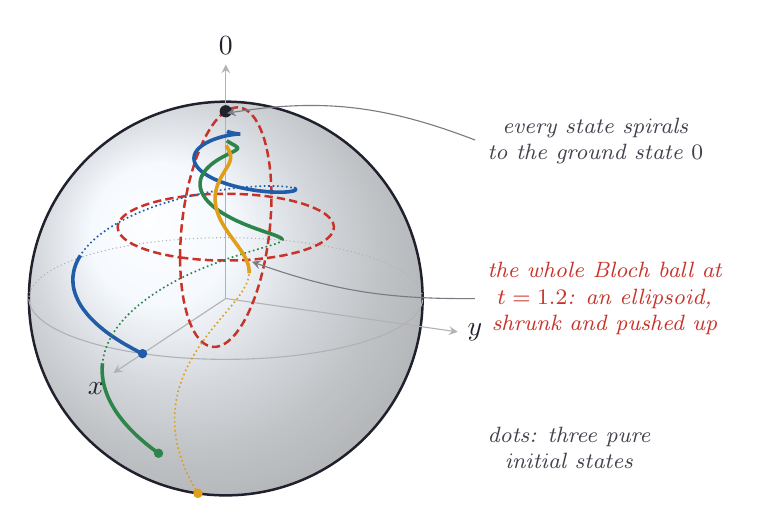
\begin{tikzpicture}[ink/.style={line width=0.9pt, ndInk}, faint/.style={line width=0.4pt, ndInk!35}, dashedink/.style={line width=0.5pt, ndInk!55, dash pattern=on 2.5pt off 2pt}, vec/.style={->, >=stealth, line width=1.2pt}, note/.style={font=\footnotesize\itshape, text=ndInk!85, align=center}, pointer/.style={->, >=stealth, line width=0.4pt, ndInk!60, shorten >=2pt, shorten <=1pt}, dot/.style={circle, fill=ndInk, inner sep=0pt, minimum size=3.4pt}, wash/.style={fill=ndSky, fill opacity=0.55}, every node/.style={text=ndInk}]
\definecolor{ndInk}{rgb}{0.13,0.13,0.18}
\definecolor{ndPaper}{rgb}{0.99,0.96,0.88}
\definecolor{ndSky}{rgb}{0.84,0.91,0.98}
\definecolor{ndRose}{rgb}{0.98,0.86,0.84}
\definecolor{ndBlue}{rgb}{0.13,0.36,0.66}
\definecolor{ndRed}{rgb}{0.78,0.20,0.16}
\definecolor{ndGold}{rgb}{0.88,0.62,0.10}
\definecolor{ndGreen}{rgb}{0.18,0.52,0.30}
\shade[ball color=ndSky!70!white, opacity=0.45] (0.000,0.000) circle (2.500);
\draw[ink] (0.000,0.000) circle (2.500);
\draw[faint] (2.266,-0.326) -- (2.293,-0.308) -- (2.318,-0.289) -- (2.342,-0.271) -- (2.364,-0.252) -- (2.384,-0.232) -- (2.403,-0.213) -- (2.420,-0.193) -- (2.436,-0.174) -- (2.450,-0.154) -- (2.462,-0.134) -- (2.473,-0.114) -- (2.481,-0.094) -- (2.488,-0.074) -- (2.494,-0.054) -- (2.498,-0.034) -- (2.500,-0.013);
\draw[faint] (-2.500,-0.007) -- (-2.498,-0.027) -- (-2.495,-0.047) -- (-2.490,-0.067) -- (-2.484,-0.087) -- (-2.476,-0.108) -- (-2.466,-0.128) -- (-2.454,-0.147) -- (-2.441,-0.167) -- (-2.426,-0.187) -- (-2.409,-0.206) -- (-2.391,-0.226) -- (-2.371,-0.245) -- (-2.349,-0.264) -- (-2.326,-0.283) -- (-2.301,-0.302) -- (-2.275,-0.320) -- (-2.247,-0.339) -- (-2.218,-0.357) -- (-2.187,-0.375) -- (-2.154,-0.392) -- (-2.120,-0.409) -- (-2.085,-0.426) -- (-2.048,-0.443) -- (-2.010,-0.460) -- (-1.970,-0.476) -- (-1.929,-0.491) -- (-1.887,-0.507) -- (-1.843,-0.522) -- (-1.798,-0.537) -- (-1.752,-0.551) -- (-1.705,-0.565) -- (-1.657,-0.579) -- (-1.607,-0.592) -- (-1.556,-0.605) -- (-1.505,-0.617) -- (-1.452,-0.629) -- (-1.398,-0.640) -- (-1.343,-0.652) -- (-1.288,-0.662) -- (-1.231,-0.672) -- (-1.174,-0.682) -- (-1.115,-0.691) -- (-1.057,-0.700) -- (-0.997,-0.708) -- (-0.937,-0.716) -- (-0.876,-0.724) -- (-0.814,-0.730) -- (-0.752,-0.737) -- (-0.689,-0.743) -- (-0.626,-0.748) -- (-0.562,-0.753) -- (-0.498,-0.757) -- (-0.434,-0.761) -- (-0.370,-0.764) -- (-0.305,-0.767) -- (-0.240,-0.769) -- (-0.174,-0.771) -- (-0.109,-0.772) -- (-0.044,-0.772) -- (0.022,-0.773) -- (0.087,-0.772) -- (0.153,-0.771) -- (0.218,-0.770) -- (0.283,-0.768) -- (0.348,-0.765) -- (0.413,-0.762) -- (0.477,-0.758) -- (0.541,-0.754) -- (0.605,-0.750) -- (0.668,-0.744) -- (0.731,-0.739) -- (0.793,-0.733) -- (0.855,-0.726) -- (0.916,-0.719) -- (0.977,-0.711) -- (1.037,-0.703) -- (1.096,-0.694) -- (1.154,-0.685) -- (1.212,-0.676) -- (1.269,-0.666) -- (1.325,-0.655) -- (1.380,-0.644) -- (1.434,-0.633) -- (1.487,-0.621) -- (1.539,-0.609) -- (1.590,-0.596) -- (1.640,-0.583) -- (1.689,-0.570) -- (1.737,-0.556) -- (1.783,-0.541) -- (1.828,-0.527) -- (1.872,-0.512) -- (1.915,-0.497) -- (1.957,-0.481) -- (1.997,-0.465) -- (2.035,-0.449) -- (2.073,-0.432) -- (2.108,-0.415) -- (2.143,-0.398) -- (2.176,-0.380) -- (2.207,-0.363) -- (2.237,-0.345) -- (2.266,-0.326);
\draw[faint, densely dotted] (2.500,0.007) -- (2.498,0.027) -- (2.495,0.047) -- (2.490,0.067) -- (2.484,0.087) -- (2.476,0.108) -- (2.466,0.128) -- (2.454,0.147) -- (2.441,0.167) -- (2.426,0.187) -- (2.409,0.206) -- (2.391,0.226) -- (2.371,0.245) -- (2.349,0.264) -- (2.326,0.283) -- (2.301,0.302) -- (2.275,0.320) -- (2.247,0.339) -- (2.218,0.357) -- (2.187,0.375) -- (2.154,0.392) -- (2.120,0.409) -- (2.085,0.426) -- (2.048,0.443) -- (2.010,0.460) -- (1.970,0.476) -- (1.929,0.491) -- (1.887,0.507) -- (1.843,0.522) -- (1.798,0.537) -- (1.752,0.551) -- (1.705,0.565) -- (1.657,0.579) -- (1.607,0.592) -- (1.556,0.605) -- (1.505,0.617) -- (1.452,0.629) -- (1.398,0.640) -- (1.343,0.652) -- (1.288,0.662) -- (1.231,0.672) -- (1.174,0.682) -- (1.115,0.691) -- (1.057,0.700) -- (0.997,0.708) -- (0.937,0.716) -- (0.876,0.724) -- (0.814,0.730) -- (0.752,0.737) -- (0.689,0.743) -- (0.626,0.748) -- (0.562,0.753) -- (0.498,0.757) -- (0.434,0.761) -- (0.370,0.764) -- (0.305,0.767) -- (0.240,0.769) -- (0.174,0.771) -- (0.109,0.772) -- (0.044,0.772) -- (-0.022,0.773) -- (-0.087,0.772) -- (-0.153,0.771) -- (-0.218,0.770) -- (-0.283,0.768) -- (-0.348,0.765) -- (-0.413,0.762) -- (-0.477,0.758) -- (-0.541,0.754) -- (-0.605,0.750) -- (-0.668,0.744) -- (-0.731,0.739) -- (-0.793,0.733) -- (-0.855,0.726) -- (-0.916,0.719) -- (-0.977,0.711) -- (-1.037,0.703) -- (-1.096,0.694) -- (-1.154,0.685) -- (-1.212,0.676) -- (-1.269,0.666) -- (-1.325,0.655) -- (-1.380,0.644) -- (-1.434,0.633) -- (-1.487,0.621) -- (-1.539,0.609) -- (-1.590,0.596) -- (-1.640,0.583) -- (-1.689,0.570) -- (-1.737,0.556) -- (-1.783,0.541) -- (-1.828,0.527) -- (-1.872,0.512) -- (-1.915,0.497) -- (-1.957,0.481) -- (-1.997,0.465) -- (-2.035,0.449) -- (-2.073,0.432) -- (-2.108,0.415) -- (-2.143,0.398) -- (-2.176,0.380) -- (-2.207,0.363) -- (-2.237,0.345) -- (-2.266,0.326) -- (-2.293,0.308) -- (-2.318,0.289) -- (-2.342,0.271) -- (-2.364,0.252) -- (-2.384,0.232) -- (-2.403,0.213) -- (-2.420,0.193) -- (-2.436,0.174) -- (-2.450,0.154) -- (-2.462,0.134) -- (-2.473,0.114) -- (-2.481,0.094) -- (-2.488,0.074) -- (-2.494,0.054) -- (-2.498,0.034) -- (-2.500,0.013);
\draw[faint, ->, >=stealth] (0.000,0.000) -- (0.000,2.972) node[above, text=ndInk] {$\ket0$};
\draw[faint, ->, >=stealth] (0.000,0.000) -- (-1.426,-0.945) node[below left, text=ndInk] {$x$};
\draw[faint, ->, >=stealth] (0.000,0.000) -- (2.946,-0.424) node[right, text=ndInk] {$y$};
\draw[line width=0.9pt, ndRed, dash pattern=on 3pt off 1.5pt] (-0.580,0.522) -- (-0.540,0.517) -- (-0.500,0.512) -- (-0.460,0.507) -- (-0.419,0.503) -- (-0.377,0.499) -- (-0.335,0.495) -- (-0.293,0.492) -- (-0.251,0.490) -- (-0.208,0.487) -- (-0.165,0.485) -- (-0.122,0.484) -- (-0.079,0.483) -- (-0.035,0.483) -- (0.008,0.482) -- (0.051,0.483) -- (0.094,0.483) -- (0.138,0.485) -- (0.181,0.486) -- (0.223,0.488) -- (0.266,0.490) -- (0.308,0.493) -- (0.350,0.496) -- (0.392,0.500) -- (0.433,0.504) -- (0.474,0.509) -- (0.515,0.513) -- (0.555,0.519) -- (0.594,0.524) -- (0.633,0.530) -- (0.671,0.537) -- (0.708,0.543) -- (0.745,0.550) -- (0.781,0.558) -- (0.816,0.566) -- (0.851,0.574) -- (0.884,0.582) -- (0.917,0.591) -- (0.949,0.600) -- (0.979,0.610) -- (1.009,0.619) -- (1.038,0.629) -- (1.066,0.639) -- (1.093,0.650) -- (1.118,0.661) -- (1.143,0.672) -- (1.166,0.683) -- (1.189,0.695) -- (1.210,0.706) -- (1.229,0.718) -- (1.248,0.730) -- (1.265,0.743) -- (1.282,0.755) -- (1.296,0.768) -- (1.310,0.780) -- (1.322,0.793) -- (1.333,0.806) -- (1.343,0.819) -- (1.351,0.832) -- (1.358,0.845) -- (1.363,0.859) -- (1.368,0.872) -- (1.370,0.885) -- (1.372,0.899) -- (1.372,0.912) -- (1.371,0.926) -- (1.368,0.939) -- (1.364,0.952) -- (1.359,0.966) -- (1.352,0.979) -- (1.344,0.992) -- (1.334,1.005) -- (1.324,1.018) -- (1.312,1.031) -- (1.298,1.044) -- (1.284,1.056) -- (1.268,1.069) -- (1.251,1.081) -- (1.232,1.093) -- (1.212,1.105) -- (1.192,1.117) -- (1.169,1.128) -- (1.146,1.139) -- (1.122,1.150) -- (1.096,1.161) -- (1.070,1.172) -- (1.042,1.182) -- (1.013,1.192) -- (0.984,1.202) -- (0.953,1.211) -- (0.921,1.221) -- (0.889,1.229) -- (0.855,1.238) -- (0.821,1.246) -- (0.786,1.254) -- (0.750,1.261) -- (0.713,1.269) -- (0.676,1.275) -- (0.638,1.282) -- (0.599,1.288) -- (0.560,1.293) -- (0.520,1.299) -- (0.480,1.304) -- (0.439,1.308) -- (0.398,1.312) -- (0.356,1.316) -- (0.314,1.319) -- (0.272,1.322) -- (0.229,1.324) -- (0.187,1.326) -- (0.144,1.328) -- (0.100,1.329) -- (0.057,1.330) -- (0.014,1.330) -- (-0.029,1.330) -- (-0.073,1.330) -- (-0.116,1.329) -- (-0.159,1.328) -- (-0.202,1.326) -- (-0.245,1.324) -- (-0.287,1.321) -- (-0.329,1.318) -- (-0.371,1.315) -- (-0.413,1.311) -- (-0.454,1.306) -- (-0.495,1.302) -- (-0.535,1.297) -- (-0.574,1.291) -- (-0.613,1.286) -- (-0.652,1.279) -- (-0.690,1.273) -- (-0.727,1.266) -- (-0.763,1.259) -- (-0.799,1.251) -- (-0.834,1.243) -- (-0.868,1.235) -- (-0.901,1.226) -- (-0.933,1.217) -- (-0.964,1.208) -- (-0.995,1.198) -- (-1.024,1.189) -- (-1.052,1.178) -- (-1.079,1.168) -- (-1.106,1.157) -- (-1.131,1.147) -- (-1.155,1.135) -- (-1.178,1.124) -- (-1.199,1.112) -- (-1.220,1.101) -- (-1.239,1.089) -- (-1.257,1.076) -- (-1.274,1.064) -- (-1.289,1.052) -- (-1.303,1.039) -- (-1.316,1.026) -- (-1.328,1.013) -- (-1.338,1.000) -- (-1.347,0.987) -- (-1.354,0.974) -- (-1.361,0.961) -- (-1.366,0.947) -- (-1.369,0.934) -- (-1.371,0.921) -- (-1.372,0.907) -- (-1.371,0.894) -- (-1.369,0.881) -- (-1.366,0.867) -- (-1.361,0.854) -- (-1.355,0.841) -- (-1.348,0.827) -- (-1.339,0.814) -- (-1.329,0.801) -- (-1.318,0.788) -- (-1.305,0.776) -- (-1.291,0.763) -- (-1.276,0.750) -- (-1.259,0.738) -- (-1.241,0.726) -- (-1.222,0.714) -- (-1.202,0.702) -- (-1.181,0.690) -- (-1.158,0.679) -- (-1.134,0.668) -- (-1.109,0.657) -- (-1.083,0.646) -- (-1.056,0.636) -- (-1.028,0.626) -- (-0.999,0.616) -- (-0.968,0.606) -- (-0.937,0.597) -- (-0.905,0.588) -- (-0.872,0.579) -- (-0.838,0.571) -- (-0.804,0.563) -- (-0.768,0.555) -- (-0.732,0.548) -- (-0.695,0.541) -- (-0.657,0.534) -- (-0.619,0.528) -- (-0.580,0.522);
\draw[line width=0.9pt, ndRed, dash pattern=on 3pt off 1.5pt] (-0.580,0.522) -- (-0.580,0.569) -- (-0.579,0.616) -- (-0.577,0.663) -- (-0.575,0.711) -- (-0.573,0.758) -- (-0.569,0.806) -- (-0.566,0.854) -- (-0.561,0.902) -- (-0.557,0.950) -- (-0.551,0.998) -- (-0.545,1.046) -- (-0.539,1.094) -- (-0.532,1.141) -- (-0.524,1.188) -- (-0.516,1.235) -- (-0.507,1.282) -- (-0.498,1.328) -- (-0.489,1.374) -- (-0.479,1.420) -- (-0.468,1.465) -- (-0.457,1.509) -- (-0.445,1.553) -- (-0.434,1.596) -- (-0.421,1.638) -- (-0.408,1.680) -- (-0.395,1.721) -- (-0.382,1.761) -- (-0.368,1.801) -- (-0.353,1.839) -- (-0.339,1.876) -- (-0.324,1.913) -- (-0.308,1.948) -- (-0.293,1.983) -- (-0.277,2.016) -- (-0.260,2.048) -- (-0.244,2.080) -- (-0.227,2.109) -- (-0.210,2.138) -- (-0.193,2.166) -- (-0.176,2.192) -- (-0.158,2.217) -- (-0.140,2.241) -- (-0.123,2.263) -- (-0.105,2.284) -- (-0.087,2.304) -- (-0.068,2.322) -- (-0.050,2.339) -- (-0.032,2.354) -- (-0.014,2.368) -- (0.005,2.381) -- (0.023,2.392) -- (0.041,2.401) -- (0.059,2.409) -- (0.078,2.416) -- (0.096,2.421) -- (0.114,2.424) -- (0.132,2.426) -- (0.149,2.427) -- (0.167,2.426) -- (0.184,2.423) -- (0.202,2.419) -- (0.219,2.414) -- (0.236,2.407) -- (0.252,2.398) -- (0.269,2.388) -- (0.285,2.377) -- (0.300,2.364) -- (0.316,2.349) -- (0.331,2.334) -- (0.346,2.316) -- (0.361,2.298) -- (0.375,2.278) -- (0.388,2.256) -- (0.402,2.233) -- (0.415,2.209) -- (0.427,2.184) -- (0.440,2.157) -- (0.451,2.129) -- (0.463,2.100) -- (0.473,2.070) -- (0.484,2.038) -- (0.494,2.006) -- (0.503,1.972) -- (0.512,1.937) -- (0.520,1.901) -- (0.528,1.865) -- (0.535,1.827) -- (0.542,1.788) -- (0.548,1.749) -- (0.554,1.708) -- (0.559,1.667) -- (0.564,1.625) -- (0.568,1.582) -- (0.571,1.539) -- (0.574,1.495) -- (0.576,1.451) -- (0.578,1.405) -- (0.579,1.360) -- (0.580,1.314) -- (0.580,1.267) -- (0.579,1.221) -- (0.578,1.173) -- (0.576,1.126) -- (0.574,1.078) -- (0.571,1.031) -- (0.568,0.983) -- (0.564,0.935) -- (0.559,0.887) -- (0.554,0.839) -- (0.548,0.791) -- (0.542,0.743) -- (0.535,0.695) -- (0.528,0.648) -- (0.520,0.601) -- (0.512,0.554) -- (0.503,0.507) -- (0.494,0.461) -- (0.484,0.416) -- (0.473,0.370) -- (0.463,0.326) -- (0.451,0.282) -- (0.440,0.238) -- (0.427,0.195) -- (0.415,0.153) -- (0.402,0.112) -- (0.388,0.072) -- (0.375,0.032) -- (0.361,-0.007) -- (0.346,-0.045) -- (0.331,-0.082) -- (0.316,-0.118) -- (0.300,-0.153) -- (0.285,-0.187) -- (0.269,-0.220) -- (0.252,-0.251) -- (0.236,-0.282) -- (0.219,-0.311) -- (0.202,-0.339) -- (0.184,-0.366) -- (0.167,-0.392) -- (0.149,-0.416) -- (0.132,-0.439) -- (0.114,-0.461) -- (0.096,-0.481) -- (0.078,-0.500) -- (0.059,-0.518) -- (0.041,-0.534) -- (0.023,-0.549) -- (0.005,-0.562) -- (-0.014,-0.574) -- (-0.032,-0.584) -- (-0.050,-0.593) -- (-0.068,-0.600) -- (-0.087,-0.606) -- (-0.105,-0.610) -- (-0.123,-0.613) -- (-0.140,-0.614) -- (-0.158,-0.614) -- (-0.176,-0.612) -- (-0.193,-0.609) -- (-0.210,-0.604) -- (-0.227,-0.598) -- (-0.244,-0.590) -- (-0.260,-0.581) -- (-0.277,-0.570) -- (-0.293,-0.558) -- (-0.308,-0.544) -- (-0.324,-0.529) -- (-0.339,-0.512) -- (-0.353,-0.494) -- (-0.368,-0.475) -- (-0.382,-0.454) -- (-0.395,-0.432) -- (-0.408,-0.409) -- (-0.421,-0.384) -- (-0.434,-0.358) -- (-0.445,-0.331) -- (-0.457,-0.302) -- (-0.468,-0.272) -- (-0.479,-0.241) -- (-0.489,-0.209) -- (-0.498,-0.176) -- (-0.507,-0.142) -- (-0.516,-0.107) -- (-0.524,-0.070) -- (-0.532,-0.033) -- (-0.539,0.005) -- (-0.545,0.044) -- (-0.551,0.084) -- (-0.557,0.125) -- (-0.561,0.167) -- (-0.566,0.209) -- (-0.569,0.252) -- (-0.573,0.296) -- (-0.575,0.340) -- (-0.577,0.385) -- (-0.579,0.430) -- (-0.580,0.476) -- (-0.580,0.522);
\draw[line width=1.3pt, ndBlue] (-1.057,-0.700) -- (-1.116,-0.671) -- (-1.173,-0.641) -- (-1.228,-0.610) -- (-1.282,-0.580) -- (-1.333,-0.549) -- (-1.382,-0.518) -- (-1.429,-0.487) -- (-1.475,-0.455) -- (-1.518,-0.424) -- (-1.559,-0.392) -- (-1.597,-0.360) -- (-1.634,-0.328) -- (-1.669,-0.295) -- (-1.701,-0.263) -- (-1.732,-0.231) -- (-1.760,-0.198) -- (-1.786,-0.166) -- (-1.811,-0.133) -- (-1.833,-0.101) -- (-1.853,-0.068) -- (-1.871,-0.036) -- (-1.886,-0.003) -- (-1.900,0.029) -- (-1.912,0.061) -- (-1.922,0.093) -- (-1.930,0.125) -- (-1.936,0.157) -- (-1.939,0.188) -- (-1.941,0.220) -- (-1.942,0.251) -- (-1.940,0.282) -- (-1.936,0.312) -- (-1.931,0.343) -- (-1.924,0.373) -- (-1.915,0.403) -- (-1.905,0.432) -- (-1.892,0.462) -- (-1.879,0.491) -- (-1.863,0.519) -- (-1.846,0.548);
\draw[line width=1.3pt, ndBlue] (0.864,1.401) -- (0.869,1.399) -- (0.874,1.396) -- (0.878,1.394) -- (0.881,1.392) -- (0.884,1.389) -- (0.885,1.387) -- (0.885,1.384) -- (0.885,1.382) -- (0.884,1.380) -- (0.882,1.377) -- (0.879,1.375) -- (0.875,1.373) -- (0.871,1.371) -- (0.865,1.369) -- (0.860,1.367) -- (0.853,1.365) -- (0.845,1.363) -- (0.837,1.362) -- (0.829,1.360) -- (0.819,1.359) -- (0.809,1.357) -- (0.798,1.356) -- (0.787,1.355) -- (0.775,1.354) -- (0.763,1.353) -- (0.750,1.352) -- (0.736,1.352) -- (0.722,1.351) -- (0.708,1.351) -- (0.693,1.351) -- (0.677,1.351) -- (0.662,1.351) -- (0.645,1.351) -- (0.629,1.351) -- (0.612,1.352) -- (0.595,1.353) -- (0.577,1.354) -- (0.559,1.355) -- (0.541,1.356) -- (0.523,1.357) -- (0.504,1.359) -- (0.485,1.361) -- (0.466,1.363) -- (0.447,1.365) -- (0.428,1.367) -- (0.409,1.369) -- (0.389,1.372) -- (0.370,1.375) -- (0.350,1.378) -- (0.330,1.381) -- (0.311,1.384) -- (0.291,1.388) -- (0.271,1.391) -- (0.252,1.395) -- (0.232,1.399) -- (0.212,1.403) -- (0.193,1.407) -- (0.174,1.412) -- (0.154,1.416) -- (0.135,1.421) -- (0.116,1.426) -- (0.098,1.431) -- (0.079,1.436) -- (0.061,1.441) -- (0.043,1.447) -- (0.025,1.452) -- (0.007,1.458) -- (-0.010,1.464) -- (-0.027,1.470) -- (-0.044,1.476) -- (-0.061,1.482) -- (-0.077,1.488) -- (-0.093,1.494) -- (-0.109,1.501) -- (-0.124,1.507) -- (-0.139,1.514) -- (-0.153,1.521) -- (-0.168,1.528) -- (-0.181,1.535) -- (-0.195,1.542) -- (-0.208,1.549) -- (-0.221,1.556) -- (-0.233,1.563) -- (-0.245,1.571) -- (-0.256,1.578) -- (-0.267,1.585) -- (-0.278,1.593) -- (-0.288,1.600) -- (-0.298,1.608) -- (-0.307,1.615) -- (-0.316,1.623) -- (-0.325,1.631) -- (-0.333,1.638) -- (-0.340,1.646) -- (-0.348,1.654) -- (-0.354,1.662) -- (-0.361,1.669) -- (-0.366,1.677) -- (-0.372,1.685) -- (-0.377,1.693) -- (-0.381,1.700) -- (-0.385,1.708) -- (-0.389,1.716) -- (-0.392,1.723) -- (-0.395,1.731) -- (-0.398,1.739) -- (-0.400,1.746) -- (-0.401,1.754) -- (-0.402,1.761) -- (-0.403,1.769) -- (-0.404,1.776) -- (-0.404,1.784) -- (-0.403,1.791) -- (-0.402,1.798) -- (-0.401,1.806) -- (-0.400,1.813) -- (-0.398,1.820) -- (-0.396,1.827) -- (-0.393,1.834) -- (-0.390,1.841) -- (-0.387,1.848) -- (-0.383,1.854) -- (-0.380,1.861) -- (-0.375,1.868) -- (-0.371,1.874) -- (-0.366,1.880) -- (-0.361,1.887) -- (-0.356,1.893) -- (-0.350,1.899) -- (-0.345,1.905) -- (-0.339,1.911) -- (-0.332,1.917) -- (-0.326,1.923) -- (-0.319,1.928) -- (-0.312,1.934) -- (-0.305,1.939) -- (-0.298,1.945) -- (-0.290,1.950) -- (-0.283,1.955) -- (-0.275,1.960) -- (-0.267,1.965) -- (-0.259,1.970) -- (-0.251,1.975) -- (-0.242,1.979) -- (-0.234,1.984) -- (-0.225,1.988) -- (-0.217,1.992) -- (-0.208,1.997) -- (-0.199,2.001) -- (-0.190,2.005) -- (-0.182,2.008) -- (-0.173,2.012) -- (-0.164,2.016) -- (-0.155,2.019) -- (-0.146,2.023) -- (-0.137,2.026) -- (-0.128,2.029) -- (-0.119,2.032) -- (-0.110,2.035) -- (-0.101,2.038) -- (-0.092,2.041) -- (-0.083,2.044) -- (-0.074,2.046) -- (-0.066,2.049) -- (-0.057,2.051) -- (-0.048,2.054) -- (-0.040,2.056) -- (-0.032,2.058) -- (-0.023,2.060) -- (-0.015,2.062) -- (-0.007,2.064) -- (0.001,2.066) -- (0.009,2.067) -- (0.017,2.069) -- (0.024,2.070) -- (0.032,2.072) -- (0.039,2.073) -- (0.046,2.075) -- (0.053,2.076) -- (0.060,2.077) -- (0.067,2.078) -- (0.073,2.079) -- (0.080,2.080) -- (0.086,2.081) -- (0.092,2.082) -- (0.098,2.083) -- (0.104,2.083) -- (0.109,2.084) -- (0.114,2.085) -- (0.120,2.085) -- (0.125,2.086) -- (0.129,2.086) -- (0.134,2.087) -- (0.138,2.087) -- (0.142,2.088) -- (0.146,2.088) -- (0.150,2.088) -- (0.154,2.088) -- (0.157,2.089) -- (0.160,2.089) -- (0.163,2.089) -- (0.166,2.089) -- (0.168,2.089) -- (0.171,2.089) -- (0.173,2.089) -- (0.175,2.090) -- (0.177,2.090) -- (0.178,2.090) -- (0.180,2.090) -- (0.181,2.090) -- (0.182,2.090) -- (0.183,2.090) -- (0.183,2.090) -- (0.184,2.090) -- (0.184,2.090) -- (0.184,2.090) -- (0.184,2.090) -- (0.184,2.090) -- (0.183,2.090) -- (0.183,2.090) -- (0.182,2.090) -- (0.181,2.090) -- (0.180,2.090) -- (0.179,2.090) -- (0.177,2.090) -- (0.176,2.090) -- (0.174,2.090) -- (0.172,2.090) -- (0.170,2.090) -- (0.168,2.091) -- (0.166,2.091) -- (0.163,2.091) -- (0.161,2.091) -- (0.158,2.092) -- (0.156,2.092) -- (0.153,2.092) -- (0.150,2.092) -- (0.147,2.093) -- (0.144,2.093) -- (0.141,2.094) -- (0.137,2.094) -- (0.134,2.095) -- (0.130,2.095) -- (0.127,2.096) -- (0.123,2.096) -- (0.120,2.097) -- (0.116,2.097) -- (0.112,2.098) -- (0.108,2.099) -- (0.104,2.100) -- (0.101,2.100) -- (0.097,2.101) -- (0.093,2.102) -- (0.089,2.103) -- (0.085,2.104) -- (0.081,2.105) -- (0.076,2.106) -- (0.072,2.107) -- (0.068,2.108) -- (0.064,2.109) -- (0.060,2.110) -- (0.056,2.111) -- (0.052,2.112) -- (0.048,2.113) -- (0.044,2.114) -- (0.040,2.116) -- (0.036,2.117) -- (0.032,2.118) -- (0.028,2.120) -- (0.024,2.121) -- (0.020,2.122) -- (0.016,2.124);
\draw[line width=0.6pt, ndBlue, densely dotted] (-1.828,0.576) -- (-1.808,0.603) -- (-1.787,0.630) -- (-1.764,0.657) -- (-1.740,0.683) -- (-1.714,0.709) -- (-1.688,0.735) -- (-1.660,0.760) -- (-1.631,0.785) -- (-1.601,0.809) -- (-1.570,0.833) -- (-1.537,0.856) -- (-1.504,0.879) -- (-1.470,0.901) -- (-1.435,0.923) -- (-1.399,0.945) -- (-1.362,0.966) -- (-1.325,0.986) -- (-1.287,1.006) -- (-1.248,1.026) -- (-1.209,1.045) -- (-1.169,1.063) -- (-1.128,1.081) -- (-1.087,1.099) -- (-1.046,1.116) -- (-1.004,1.133) -- (-0.962,1.149) -- (-0.919,1.164) -- (-0.877,1.179) -- (-0.834,1.194) -- (-0.791,1.208) -- (-0.748,1.221) -- (-0.705,1.234) -- (-0.661,1.247) -- (-0.618,1.259) -- (-0.575,1.271) -- (-0.532,1.282) -- (-0.489,1.293) -- (-0.446,1.303) -- (-0.404,1.313) -- (-0.362,1.322) -- (-0.320,1.331) -- (-0.278,1.339) -- (-0.237,1.347) -- (-0.196,1.355) -- (-0.155,1.362) -- (-0.115,1.369) -- (-0.076,1.375) -- (-0.037,1.381) -- (0.002,1.387) -- (0.040,1.392) -- (0.077,1.397) -- (0.114,1.401) -- (0.150,1.405) -- (0.185,1.409) -- (0.220,1.412) -- (0.254,1.415) -- (0.287,1.418) -- (0.319,1.420) -- (0.351,1.422) -- (0.382,1.424) -- (0.412,1.426) -- (0.441,1.427) -- (0.469,1.428) -- (0.496,1.429) -- (0.523,1.429) -- (0.549,1.430) -- (0.573,1.430) -- (0.597,1.429) -- (0.620,1.429) -- (0.642,1.428) -- (0.663,1.428) -- (0.683,1.427) -- (0.702,1.426) -- (0.720,1.424) -- (0.738,1.423) -- (0.754,1.422) -- (0.769,1.420) -- (0.783,1.418) -- (0.797,1.416) -- (0.809,1.414) -- (0.821,1.412) -- (0.831,1.410) -- (0.841,1.408) -- (0.849,1.406) -- (0.857,1.403);
\node[dot, fill=ndBlue] at (-1.057,-0.700) {};
\draw[line width=1.3pt, ndGreen] (-0.854,-1.965) -- (-0.902,-1.930) -- (-0.948,-1.895) -- (-0.993,-1.860) -- (-1.036,-1.824) -- (-1.078,-1.788) -- (-1.118,-1.752) -- (-1.156,-1.716) -- (-1.192,-1.680) -- (-1.227,-1.644) -- (-1.260,-1.608) -- (-1.292,-1.571) -- (-1.321,-1.535) -- (-1.349,-1.499) -- (-1.376,-1.462) -- (-1.400,-1.426) -- (-1.423,-1.389) -- (-1.444,-1.353) -- (-1.464,-1.317) -- (-1.482,-1.280) -- (-1.498,-1.244) -- (-1.512,-1.208) -- (-1.525,-1.172) -- (-1.536,-1.136) -- (-1.546,-1.101) -- (-1.554,-1.065) -- (-1.560,-1.030) -- (-1.565,-0.995) -- (-1.568,-0.960) -- (-1.570,-0.925) -- (-1.570,-0.890) -- (-1.568,-0.856) -- (-1.566,-0.822);
\draw[line width=1.3pt, ndGreen] (0.714,0.740) -- (0.715,0.743) -- (0.716,0.746) -- (0.715,0.749) -- (0.714,0.752) -- (0.713,0.756) -- (0.710,0.759) -- (0.708,0.762) -- (0.704,0.765) -- (0.700,0.768) -- (0.695,0.771) -- (0.690,0.774) -- (0.684,0.778) -- (0.677,0.781) -- (0.670,0.784) -- (0.662,0.788) -- (0.654,0.791) -- (0.645,0.795) -- (0.636,0.798) -- (0.627,0.802) -- (0.617,0.806) -- (0.606,0.810) -- (0.595,0.814) -- (0.584,0.818) -- (0.572,0.822) -- (0.560,0.826) -- (0.548,0.830) -- (0.535,0.835) -- (0.522,0.839) -- (0.508,0.844) -- (0.495,0.848) -- (0.481,0.853) -- (0.467,0.858) -- (0.452,0.863) -- (0.438,0.868) -- (0.423,0.874) -- (0.408,0.879) -- (0.392,0.884) -- (0.377,0.890) -- (0.362,0.896) -- (0.346,0.902) -- (0.330,0.907) -- (0.315,0.913) -- (0.299,0.920) -- (0.283,0.926) -- (0.267,0.932) -- (0.251,0.939) -- (0.235,0.945) -- (0.219,0.952) -- (0.203,0.959) -- (0.188,0.966) -- (0.172,0.973) -- (0.156,0.980) -- (0.140,0.987) -- (0.125,0.994) -- (0.109,1.002) -- (0.094,1.009) -- (0.079,1.017) -- (0.064,1.025) -- (0.049,1.033) -- (0.035,1.041) -- (0.020,1.048) -- (0.006,1.057) -- (-0.008,1.065) -- (-0.022,1.073) -- (-0.036,1.081) -- (-0.049,1.090) -- (-0.062,1.098) -- (-0.075,1.107) -- (-0.088,1.115) -- (-0.100,1.124) -- (-0.112,1.133) -- (-0.124,1.141) -- (-0.136,1.150) -- (-0.147,1.159) -- (-0.158,1.168) -- (-0.168,1.177) -- (-0.178,1.186) -- (-0.188,1.195) -- (-0.198,1.204) -- (-0.207,1.213) -- (-0.216,1.222) -- (-0.225,1.231) -- (-0.233,1.240) -- (-0.241,1.249) -- (-0.248,1.259) -- (-0.256,1.268) -- (-0.263,1.277) -- (-0.269,1.286) -- (-0.275,1.295) -- (-0.281,1.305) -- (-0.286,1.314) -- (-0.291,1.323) -- (-0.296,1.332) -- (-0.301,1.341) -- (-0.305,1.350) -- (-0.308,1.359) -- (-0.312,1.369) -- (-0.315,1.378) -- (-0.317,1.387) -- (-0.320,1.396) -- (-0.322,1.404) -- (-0.323,1.413) -- (-0.324,1.422) -- (-0.325,1.431) -- (-0.326,1.440) -- (-0.326,1.448) -- (-0.326,1.457) -- (-0.326,1.466) -- (-0.325,1.474) -- (-0.324,1.483) -- (-0.323,1.491) -- (-0.322,1.499) -- (-0.320,1.508) -- (-0.318,1.516) -- (-0.316,1.524) -- (-0.313,1.532) -- (-0.310,1.540) -- (-0.307,1.548) -- (-0.304,1.555) -- (-0.300,1.563) -- (-0.296,1.571) -- (-0.292,1.578) -- (-0.288,1.586) -- (-0.283,1.593) -- (-0.279,1.600) -- (-0.274,1.608) -- (-0.269,1.615) -- (-0.263,1.622) -- (-0.258,1.629) -- (-0.252,1.635) -- (-0.247,1.642) -- (-0.241,1.649) -- (-0.235,1.655) -- (-0.228,1.662) -- (-0.222,1.668) -- (-0.216,1.674) -- (-0.209,1.680) -- (-0.203,1.686) -- (-0.196,1.692) -- (-0.189,1.698) -- (-0.182,1.704) -- (-0.175,1.709) -- (-0.168,1.715) -- (-0.161,1.720) -- (-0.154,1.726) -- (-0.147,1.731) -- (-0.140,1.736) -- (-0.132,1.741) -- (-0.125,1.746) -- (-0.118,1.751) -- (-0.111,1.755) -- (-0.103,1.760) -- (-0.096,1.764) -- (-0.089,1.769) -- (-0.082,1.773) -- (-0.074,1.777) -- (-0.067,1.782) -- (-0.060,1.786) -- (-0.053,1.790) -- (-0.046,1.794) -- (-0.039,1.797) -- (-0.032,1.801) -- (-0.026,1.805) -- (-0.019,1.808) -- (-0.012,1.812) -- (-0.006,1.815) -- (0.001,1.818) -- (0.007,1.822) -- (0.013,1.825) -- (0.020,1.828) -- (0.026,1.831) -- (0.032,1.834) -- (0.037,1.837) -- (0.043,1.839) -- (0.049,1.842) -- (0.054,1.845) -- (0.059,1.847) -- (0.065,1.850) -- (0.070,1.852) -- (0.074,1.855) -- (0.079,1.857) -- (0.084,1.859) -- (0.088,1.861) -- (0.093,1.864) -- (0.097,1.866) -- (0.101,1.868) -- (0.105,1.870) -- (0.108,1.872) -- (0.112,1.874) -- (0.115,1.876) -- (0.118,1.878) -- (0.121,1.879) -- (0.124,1.881) -- (0.127,1.883) -- (0.129,1.885) -- (0.132,1.886) -- (0.134,1.888) -- (0.136,1.890) -- (0.138,1.891) -- (0.140,1.893) -- (0.141,1.894) -- (0.143,1.896) -- (0.144,1.898) -- (0.145,1.899) -- (0.146,1.901) -- (0.147,1.902) -- (0.148,1.903) -- (0.148,1.905) -- (0.149,1.906) -- (0.149,1.908) -- (0.149,1.909) -- (0.149,1.911) -- (0.149,1.912) -- (0.148,1.913) -- (0.148,1.915) -- (0.147,1.916) -- (0.146,1.918) -- (0.145,1.919) -- (0.144,1.920) -- (0.143,1.922) -- (0.142,1.923) -- (0.141,1.925) -- (0.139,1.926) -- (0.138,1.928) -- (0.136,1.929) -- (0.134,1.930) -- (0.132,1.932) -- (0.130,1.933) -- (0.128,1.935) -- (0.126,1.936) -- (0.124,1.938) -- (0.121,1.939) -- (0.119,1.941) -- (0.116,1.943) -- (0.114,1.944) -- (0.111,1.946) -- (0.108,1.947) -- (0.105,1.949) -- (0.103,1.951) -- (0.100,1.952) -- (0.097,1.954) -- (0.094,1.956) -- (0.091,1.957) -- (0.088,1.959) -- (0.084,1.961) -- (0.081,1.963) -- (0.078,1.964) -- (0.075,1.966) -- (0.072,1.968) -- (0.068,1.970) -- (0.065,1.972) -- (0.062,1.974) -- (0.059,1.975) -- (0.055,1.977) -- (0.052,1.979) -- (0.049,1.981) -- (0.045,1.983) -- (0.042,1.985) -- (0.039,1.987) -- (0.035,1.989) -- (0.032,1.991) -- (0.029,1.994) -- (0.026,1.996) -- (0.022,1.998) -- (0.019,2.000) -- (0.016,2.002) -- (0.013,2.004);
\draw[line width=0.6pt, ndGreen, densely dotted] (-1.561,-0.788) -- (-1.556,-0.755) -- (-1.548,-0.721) -- (-1.540,-0.689) -- (-1.530,-0.656) -- (-1.519,-0.624) -- (-1.506,-0.592) -- (-1.493,-0.560) -- (-1.478,-0.529) -- (-1.462,-0.498) -- (-1.444,-0.467) -- (-1.426,-0.437) -- (-1.407,-0.407) -- (-1.386,-0.377) -- (-1.365,-0.348) -- (-1.342,-0.320) -- (-1.319,-0.291) -- (-1.294,-0.263) -- (-1.269,-0.236) -- (-1.243,-0.209) -- (-1.216,-0.182) -- (-1.189,-0.156) -- (-1.160,-0.130) -- (-1.131,-0.105) -- (-1.102,-0.080) -- (-1.071,-0.056) -- (-1.040,-0.032) -- (-1.009,-0.008) -- (-0.977,0.015) -- (-0.945,0.038) -- (-0.912,0.060) -- (-0.879,0.082) -- (-0.845,0.103) -- (-0.812,0.124) -- (-0.778,0.145) -- (-0.743,0.165) -- (-0.709,0.184) -- (-0.674,0.203) -- (-0.639,0.222) -- (-0.605,0.240) -- (-0.570,0.258) -- (-0.535,0.275) -- (-0.500,0.292) -- (-0.465,0.309) -- (-0.430,0.325) -- (-0.395,0.340) -- (-0.361,0.356) -- (-0.327,0.370) -- (-0.292,0.385) -- (-0.258,0.399) -- (-0.225,0.412) -- (-0.191,0.426) -- (-0.158,0.439) -- (-0.125,0.451) -- (-0.093,0.463) -- (-0.061,0.475) -- (-0.030,0.486) -- (0.002,0.497) -- (0.032,0.508) -- (0.062,0.518) -- (0.092,0.528) -- (0.121,0.538) -- (0.150,0.547) -- (0.178,0.556) -- (0.205,0.565) -- (0.232,0.573) -- (0.258,0.581) -- (0.284,0.589) -- (0.309,0.597) -- (0.333,0.604) -- (0.356,0.611) -- (0.379,0.618) -- (0.401,0.624) -- (0.423,0.631) -- (0.444,0.637) -- (0.464,0.643) -- (0.483,0.648) -- (0.501,0.654) -- (0.519,0.659) -- (0.536,0.664) -- (0.552,0.669) -- (0.568,0.674) -- (0.582,0.678) -- (0.596,0.683) -- (0.609,0.687) -- (0.622,0.691) -- (0.633,0.695) -- (0.644,0.699) -- (0.654,0.703) -- (0.663,0.707) -- (0.672,0.710) -- (0.680,0.714) -- (0.687,0.717) -- (0.693,0.721) -- (0.698,0.724) -- (0.703,0.727) -- (0.707,0.731) -- (0.710,0.734) -- (0.713,0.737);
\node[dot, fill=ndGreen] at (-0.854,-1.965) {};
\draw[line width=1.3pt, ndGold] (0.296,0.319) -- (0.296,0.329) -- (0.297,0.338) -- (0.296,0.348) -- (0.296,0.357) -- (0.295,0.366) -- (0.294,0.376) -- (0.293,0.385) -- (0.292,0.394) -- (0.290,0.403) -- (0.288,0.413) -- (0.286,0.422) -- (0.283,0.431) -- (0.280,0.440) -- (0.278,0.449) -- (0.274,0.458) -- (0.271,0.467) -- (0.267,0.476) -- (0.264,0.485) -- (0.260,0.494) -- (0.256,0.503) -- (0.251,0.512) -- (0.247,0.521) -- (0.242,0.530) -- (0.237,0.538) -- (0.232,0.547) -- (0.227,0.556) -- (0.222,0.565) -- (0.216,0.574) -- (0.211,0.583) -- (0.205,0.592) -- (0.199,0.601) -- (0.193,0.610) -- (0.187,0.619) -- (0.181,0.627) -- (0.175,0.636) -- (0.169,0.645) -- (0.163,0.654) -- (0.156,0.663) -- (0.150,0.672) -- (0.143,0.681) -- (0.137,0.690) -- (0.130,0.699) -- (0.124,0.708) -- (0.117,0.717) -- (0.111,0.726) -- (0.104,0.735) -- (0.097,0.744) -- (0.091,0.753) -- (0.084,0.762) -- (0.078,0.771) -- (0.071,0.780) -- (0.065,0.789) -- (0.058,0.798) -- (0.052,0.807) -- (0.045,0.816) -- (0.039,0.825) -- (0.033,0.834) -- (0.027,0.843) -- (0.020,0.853) -- (0.014,0.862) -- (0.008,0.871) -- (0.002,0.880) -- (-0.003,0.889) -- (-0.009,0.898) -- (-0.015,0.907) -- (-0.020,0.916) -- (-0.026,0.925) -- (-0.031,0.934) -- (-0.036,0.943) -- (-0.042,0.952) -- (-0.047,0.961) -- (-0.051,0.970) -- (-0.056,0.979) -- (-0.061,0.988) -- (-0.065,0.997) -- (-0.070,1.006) -- (-0.074,1.015) -- (-0.078,1.024) -- (-0.082,1.033) -- (-0.086,1.042) -- (-0.090,1.051) -- (-0.093,1.060) -- (-0.097,1.069) -- (-0.100,1.078) -- (-0.103,1.086) -- (-0.106,1.095) -- (-0.109,1.104) -- (-0.111,1.113) -- (-0.114,1.121) -- (-0.116,1.130) -- (-0.119,1.139) -- (-0.121,1.147) -- (-0.123,1.156) -- (-0.125,1.164) -- (-0.126,1.173) -- (-0.128,1.181) -- (-0.129,1.189) -- (-0.130,1.198) -- (-0.131,1.206) -- (-0.132,1.214) -- (-0.133,1.223) -- (-0.134,1.231) -- (-0.134,1.239) -- (-0.135,1.247) -- (-0.135,1.255) -- (-0.135,1.263) -- (-0.135,1.271) -- (-0.135,1.279) -- (-0.135,1.287) -- (-0.134,1.295) -- (-0.134,1.302) -- (-0.133,1.310) -- (-0.133,1.318) -- (-0.132,1.325) -- (-0.131,1.333) -- (-0.130,1.340) -- (-0.128,1.348) -- (-0.127,1.355) -- (-0.126,1.362) -- (-0.124,1.370) -- (-0.123,1.377) -- (-0.121,1.384) -- (-0.119,1.391) -- (-0.117,1.398) -- (-0.115,1.405) -- (-0.113,1.412) -- (-0.111,1.419) -- (-0.109,1.425) -- (-0.107,1.432) -- (-0.105,1.439) -- (-0.102,1.445) -- (-0.100,1.452) -- (-0.097,1.458) -- (-0.095,1.465) -- (-0.092,1.471) -- (-0.089,1.477) -- (-0.087,1.483) -- (-0.084,1.489) -- (-0.081,1.495) -- (-0.078,1.501) -- (-0.075,1.507) -- (-0.073,1.513) -- (-0.070,1.519) -- (-0.067,1.525) -- (-0.064,1.531) -- (-0.061,1.536) -- (-0.058,1.542) -- (-0.055,1.547) -- (-0.052,1.553) -- (-0.049,1.558) -- (-0.046,1.563) -- (-0.043,1.569) -- (-0.040,1.574) -- (-0.037,1.579) -- (-0.034,1.584) -- (-0.031,1.589) -- (-0.028,1.594) -- (-0.025,1.599) -- (-0.022,1.604) -- (-0.019,1.608) -- (-0.016,1.613) -- (-0.013,1.618) -- (-0.011,1.623) -- (-0.008,1.627) -- (-0.005,1.632) -- (-0.002,1.636) -- (0.000,1.640) -- (0.003,1.645) -- (0.006,1.649) -- (0.008,1.653) -- (0.011,1.658) -- (0.013,1.662) -- (0.016,1.666) -- (0.018,1.670) -- (0.020,1.674) -- (0.022,1.678) -- (0.025,1.682) -- (0.027,1.686) -- (0.029,1.690) -- (0.031,1.694) -- (0.033,1.697) -- (0.035,1.701) -- (0.037,1.705) -- (0.038,1.708) -- (0.040,1.712) -- (0.042,1.716) -- (0.043,1.719) -- (0.045,1.723) -- (0.046,1.726) -- (0.048,1.730) -- (0.049,1.733) -- (0.050,1.736) -- (0.051,1.740) -- (0.053,1.743) -- (0.054,1.746) -- (0.055,1.750) -- (0.056,1.753) -- (0.056,1.756) -- (0.057,1.759) -- (0.058,1.762) -- (0.059,1.766) -- (0.059,1.769) -- (0.060,1.772) -- (0.060,1.775) -- (0.061,1.778) -- (0.061,1.781) -- (0.061,1.784) -- (0.061,1.787) -- (0.062,1.790) -- (0.062,1.793) -- (0.062,1.796) -- (0.062,1.799) -- (0.062,1.801) -- (0.061,1.804) -- (0.061,1.807) -- (0.061,1.810) -- (0.061,1.813) -- (0.060,1.816) -- (0.060,1.819) -- (0.059,1.821) -- (0.059,1.824) -- (0.058,1.827) -- (0.058,1.830) -- (0.057,1.832) -- (0.056,1.835) -- (0.056,1.838) -- (0.055,1.841) -- (0.054,1.843) -- (0.053,1.846) -- (0.052,1.849) -- (0.051,1.852) -- (0.050,1.854) -- (0.049,1.857) -- (0.048,1.860) -- (0.047,1.862) -- (0.046,1.865) -- (0.045,1.868) -- (0.044,1.870) -- (0.043,1.873) -- (0.041,1.876) -- (0.040,1.878) -- (0.039,1.881) -- (0.038,1.883) -- (0.036,1.886) -- (0.035,1.889) -- (0.034,1.891) -- (0.032,1.894) -- (0.031,1.897) -- (0.030,1.899) -- (0.028,1.902) -- (0.027,1.904) -- (0.026,1.907) -- (0.024,1.910) -- (0.023,1.912) -- (0.022,1.915) -- (0.020,1.918) -- (0.019,1.920) -- (0.017,1.923) -- (0.016,1.925) -- (0.015,1.928) -- (0.013,1.930) -- (0.012,1.933) -- (0.011,1.936) -- (0.009,1.938) -- (0.008,1.941) -- (0.007,1.943) -- (0.005,1.946);
\draw[line width=0.6pt, ndGold, densely dotted] (-0.354,-2.475) -- (-0.374,-2.442) -- (-0.393,-2.409) -- (-0.411,-2.376) -- (-0.429,-2.344) -- (-0.447,-2.311) -- (-0.463,-2.278) -- (-0.479,-2.246) -- (-0.494,-2.213) -- (-0.508,-2.181) -- (-0.522,-2.148) -- (-0.535,-2.116) -- (-0.547,-2.084) -- (-0.559,-2.052) -- (-0.570,-2.020) -- (-0.580,-1.988) -- (-0.590,-1.956) -- (-0.598,-1.924) -- (-0.607,-1.893) -- (-0.614,-1.861) -- (-0.621,-1.830) -- (-0.627,-1.799) -- (-0.632,-1.768) -- (-0.637,-1.737) -- (-0.641,-1.706) -- (-0.644,-1.676) -- (-0.646,-1.645) -- (-0.648,-1.615) -- (-0.650,-1.585) -- (-0.650,-1.555) -- (-0.650,-1.525) -- (-0.650,-1.496) -- (-0.649,-1.467) -- (-0.647,-1.437) -- (-0.644,-1.409) -- (-0.642,-1.380) -- (-0.638,-1.351) -- (-0.634,-1.323) -- (-0.629,-1.295) -- (-0.624,-1.267) -- (-0.618,-1.240) -- (-0.612,-1.212) -- (-0.606,-1.185) -- (-0.598,-1.158) -- (-0.591,-1.132) -- (-0.583,-1.105) -- (-0.574,-1.079) -- (-0.565,-1.053) -- (-0.556,-1.027) -- (-0.546,-1.002) -- (-0.536,-0.977) -- (-0.526,-0.952) -- (-0.515,-0.927) -- (-0.504,-0.903) -- (-0.492,-0.878) -- (-0.481,-0.855) -- (-0.469,-0.831) -- (-0.456,-0.808) -- (-0.444,-0.784) -- (-0.431,-0.762) -- (-0.418,-0.739) -- (-0.405,-0.717) -- (-0.391,-0.694) -- (-0.378,-0.673) -- (-0.364,-0.651) -- (-0.350,-0.630) -- (-0.336,-0.609) -- (-0.322,-0.588) -- (-0.308,-0.567) -- (-0.294,-0.547) -- (-0.279,-0.527) -- (-0.265,-0.507) -- (-0.251,-0.488) -- (-0.236,-0.469) -- (-0.222,-0.450) -- (-0.207,-0.431) -- (-0.193,-0.412) -- (-0.178,-0.394) -- (-0.164,-0.376) -- (-0.150,-0.358) -- (-0.135,-0.341) -- (-0.121,-0.324) -- (-0.107,-0.307) -- (-0.093,-0.290) -- (-0.079,-0.273) -- (-0.066,-0.257) -- (-0.052,-0.241) -- (-0.039,-0.225) -- (-0.025,-0.209) -- (-0.012,-0.194) -- (0.001,-0.178) -- (0.013,-0.163) -- (0.026,-0.148) -- (0.038,-0.134) -- (0.050,-0.119) -- (0.062,-0.105) -- (0.074,-0.091) -- (0.085,-0.077) -- (0.096,-0.063) -- (0.107,-0.050) -- (0.118,-0.036) -- (0.128,-0.023) -- (0.138,-0.010) -- (0.148,0.003) -- (0.157,0.015) -- (0.166,0.028) -- (0.175,0.040) -- (0.184,0.052) -- (0.192,0.064) -- (0.200,0.076) -- (0.208,0.088) -- (0.215,0.100) -- (0.222,0.111) -- (0.229,0.123) -- (0.235,0.134) -- (0.241,0.145) -- (0.247,0.156) -- (0.253,0.167) -- (0.258,0.178) -- (0.262,0.188) -- (0.267,0.199) -- (0.271,0.209) -- (0.275,0.220) -- (0.278,0.230) -- (0.282,0.240) -- (0.284,0.250) -- (0.287,0.260) -- (0.289,0.270) -- (0.291,0.280) -- (0.293,0.290) -- (0.294,0.300) -- (0.295,0.309);
\node[dot, fill=ndGold] at (-0.354,-2.475) {};
\node[dot, fill=ndInk, minimum size=4.4pt] at (0.000,2.378) {};
\node[note, anchor=west] (a) at (3.20,2.0) {every state spirals\\ to the ground state $\ket0$};
\draw[pointer] (a.west) to[bend right=15] (-0.053,2.343);
\node[note, anchor=west, text=ndRed] (e) at (3.20,0.0) {the whole Bloch ball at\\ $t=1.2$: an ellipsoid,\\ shrunk and pushed up};
\draw[pointer] (e.west) to[bend left=10] (0.266,0.490);
\node[note, anchor=west] at (3.20,-1.9) {dots: three pure\\ initial states};
\end{tikzpicture}
}
\caption{Three initial pure states (dots) under the same dissipative dynamics as in Figure~\ref{fig:ch03:decoherence}: every trajectory leaves the sphere, spirals inwards and converges to the ground state at the north pole. Red: the image of the whole Bloch ball at $t=1.2$, the ellipsoid with semi-axes $\ee^{-t/T_2}$, $\ee^{-t/T_2}$, $\ee^{-t/T_1}$ centred at $z=1-\ee^{-t/T_1}$: the channel contracts the ball and pushes it towards the ground state. Generated by \texttt{code/ch03\_decoherence.py}.}\label{fig:ch03:shrink}
\end{figure}}
\ona{\endgraf\medskip\noindent\textit{Reading the figure.} The sphere is the set of pure states. Each coloured curve is the Bloch vector of one initial state (the dot) as time goes on: it leaves the surface, so the state becomes mixed, spirals because of the precession, and ends at the north pole, the ground state $\ket0$. The red dashed ellipsoid shows where \emph{all} points of the Bloch ball are at time $t=1.2$: the whole ball has been squeezed and moved up.\endgraf\smallskip\noindent\textit{Why it matters.} Unitary dynamics (\Chap~\ref{C.Closed}) only rotate the ball. Open dynamics \emph{contract} it, so that different initial states become harder to tell apart: information leaks into the environment. A computer scientist will recognise the behaviour of a Markov chain converging to its stationary distribution irrespective of where it started; here the ground state plays the role of the stationary distribution. The ellipsoid is not centred at the origin: the map is \emph{affine}, a linear map followed by a shift, and the shift is the origin of the affine term $\bvec$ in Theorem~\ref{thm:ch03:blds}.}
\onp{\begin{center}\resizebox{!}{0.6\textheight}{% Generated by code/needham.py -- do not edit by hand.
\definecolor{qocA}{rgb}{0.00,0.45,0.70}
\definecolor{qocB}{rgb}{0.90,0.60,0.00}
\definecolor{qocC}{rgb}{0.00,0.62,0.45}
\definecolor{qocD}{rgb}{0.80,0.40,0.00}
\definecolor{qocE}{rgb}{0.80,0.60,0.70}
\definecolor{qocF}{rgb}{0.35,0.70,0.90}
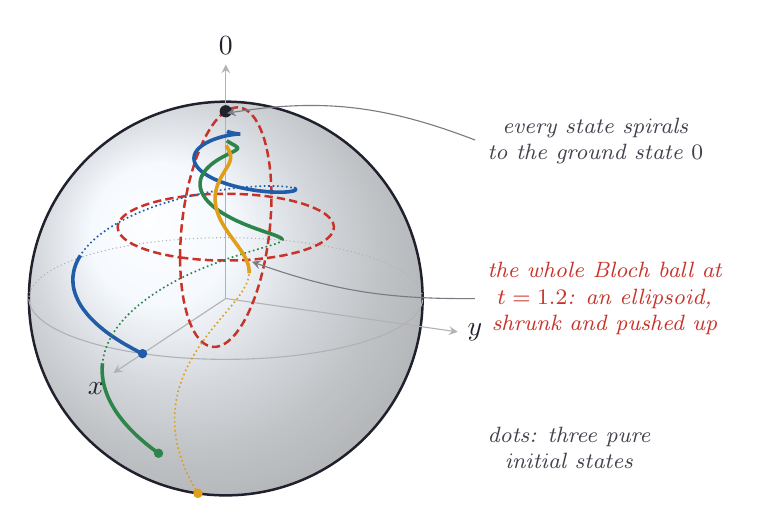
\begin{tikzpicture}[ink/.style={line width=0.9pt, ndInk}, faint/.style={line width=0.4pt, ndInk!35}, dashedink/.style={line width=0.5pt, ndInk!55, dash pattern=on 2.5pt off 2pt}, vec/.style={->, >=stealth, line width=1.2pt}, note/.style={font=\footnotesize\itshape, text=ndInk!85, align=center}, pointer/.style={->, >=stealth, line width=0.4pt, ndInk!60, shorten >=2pt, shorten <=1pt}, dot/.style={circle, fill=ndInk, inner sep=0pt, minimum size=3.4pt}, wash/.style={fill=ndSky, fill opacity=0.55}, every node/.style={text=ndInk}]
\definecolor{ndInk}{rgb}{0.13,0.13,0.18}
\definecolor{ndPaper}{rgb}{0.99,0.96,0.88}
\definecolor{ndSky}{rgb}{0.84,0.91,0.98}
\definecolor{ndRose}{rgb}{0.98,0.86,0.84}
\definecolor{ndBlue}{rgb}{0.13,0.36,0.66}
\definecolor{ndRed}{rgb}{0.78,0.20,0.16}
\definecolor{ndGold}{rgb}{0.88,0.62,0.10}
\definecolor{ndGreen}{rgb}{0.18,0.52,0.30}
\shade[ball color=ndSky!70!white, opacity=0.45] (0.000,0.000) circle (2.500);
\draw[ink] (0.000,0.000) circle (2.500);
\draw[faint] (2.266,-0.326) -- (2.293,-0.308) -- (2.318,-0.289) -- (2.342,-0.271) -- (2.364,-0.252) -- (2.384,-0.232) -- (2.403,-0.213) -- (2.420,-0.193) -- (2.436,-0.174) -- (2.450,-0.154) -- (2.462,-0.134) -- (2.473,-0.114) -- (2.481,-0.094) -- (2.488,-0.074) -- (2.494,-0.054) -- (2.498,-0.034) -- (2.500,-0.013);
\draw[faint] (-2.500,-0.007) -- (-2.498,-0.027) -- (-2.495,-0.047) -- (-2.490,-0.067) -- (-2.484,-0.087) -- (-2.476,-0.108) -- (-2.466,-0.128) -- (-2.454,-0.147) -- (-2.441,-0.167) -- (-2.426,-0.187) -- (-2.409,-0.206) -- (-2.391,-0.226) -- (-2.371,-0.245) -- (-2.349,-0.264) -- (-2.326,-0.283) -- (-2.301,-0.302) -- (-2.275,-0.320) -- (-2.247,-0.339) -- (-2.218,-0.357) -- (-2.187,-0.375) -- (-2.154,-0.392) -- (-2.120,-0.409) -- (-2.085,-0.426) -- (-2.048,-0.443) -- (-2.010,-0.460) -- (-1.970,-0.476) -- (-1.929,-0.491) -- (-1.887,-0.507) -- (-1.843,-0.522) -- (-1.798,-0.537) -- (-1.752,-0.551) -- (-1.705,-0.565) -- (-1.657,-0.579) -- (-1.607,-0.592) -- (-1.556,-0.605) -- (-1.505,-0.617) -- (-1.452,-0.629) -- (-1.398,-0.640) -- (-1.343,-0.652) -- (-1.288,-0.662) -- (-1.231,-0.672) -- (-1.174,-0.682) -- (-1.115,-0.691) -- (-1.057,-0.700) -- (-0.997,-0.708) -- (-0.937,-0.716) -- (-0.876,-0.724) -- (-0.814,-0.730) -- (-0.752,-0.737) -- (-0.689,-0.743) -- (-0.626,-0.748) -- (-0.562,-0.753) -- (-0.498,-0.757) -- (-0.434,-0.761) -- (-0.370,-0.764) -- (-0.305,-0.767) -- (-0.240,-0.769) -- (-0.174,-0.771) -- (-0.109,-0.772) -- (-0.044,-0.772) -- (0.022,-0.773) -- (0.087,-0.772) -- (0.153,-0.771) -- (0.218,-0.770) -- (0.283,-0.768) -- (0.348,-0.765) -- (0.413,-0.762) -- (0.477,-0.758) -- (0.541,-0.754) -- (0.605,-0.750) -- (0.668,-0.744) -- (0.731,-0.739) -- (0.793,-0.733) -- (0.855,-0.726) -- (0.916,-0.719) -- (0.977,-0.711) -- (1.037,-0.703) -- (1.096,-0.694) -- (1.154,-0.685) -- (1.212,-0.676) -- (1.269,-0.666) -- (1.325,-0.655) -- (1.380,-0.644) -- (1.434,-0.633) -- (1.487,-0.621) -- (1.539,-0.609) -- (1.590,-0.596) -- (1.640,-0.583) -- (1.689,-0.570) -- (1.737,-0.556) -- (1.783,-0.541) -- (1.828,-0.527) -- (1.872,-0.512) -- (1.915,-0.497) -- (1.957,-0.481) -- (1.997,-0.465) -- (2.035,-0.449) -- (2.073,-0.432) -- (2.108,-0.415) -- (2.143,-0.398) -- (2.176,-0.380) -- (2.207,-0.363) -- (2.237,-0.345) -- (2.266,-0.326);
\draw[faint, densely dotted] (2.500,0.007) -- (2.498,0.027) -- (2.495,0.047) -- (2.490,0.067) -- (2.484,0.087) -- (2.476,0.108) -- (2.466,0.128) -- (2.454,0.147) -- (2.441,0.167) -- (2.426,0.187) -- (2.409,0.206) -- (2.391,0.226) -- (2.371,0.245) -- (2.349,0.264) -- (2.326,0.283) -- (2.301,0.302) -- (2.275,0.320) -- (2.247,0.339) -- (2.218,0.357) -- (2.187,0.375) -- (2.154,0.392) -- (2.120,0.409) -- (2.085,0.426) -- (2.048,0.443) -- (2.010,0.460) -- (1.970,0.476) -- (1.929,0.491) -- (1.887,0.507) -- (1.843,0.522) -- (1.798,0.537) -- (1.752,0.551) -- (1.705,0.565) -- (1.657,0.579) -- (1.607,0.592) -- (1.556,0.605) -- (1.505,0.617) -- (1.452,0.629) -- (1.398,0.640) -- (1.343,0.652) -- (1.288,0.662) -- (1.231,0.672) -- (1.174,0.682) -- (1.115,0.691) -- (1.057,0.700) -- (0.997,0.708) -- (0.937,0.716) -- (0.876,0.724) -- (0.814,0.730) -- (0.752,0.737) -- (0.689,0.743) -- (0.626,0.748) -- (0.562,0.753) -- (0.498,0.757) -- (0.434,0.761) -- (0.370,0.764) -- (0.305,0.767) -- (0.240,0.769) -- (0.174,0.771) -- (0.109,0.772) -- (0.044,0.772) -- (-0.022,0.773) -- (-0.087,0.772) -- (-0.153,0.771) -- (-0.218,0.770) -- (-0.283,0.768) -- (-0.348,0.765) -- (-0.413,0.762) -- (-0.477,0.758) -- (-0.541,0.754) -- (-0.605,0.750) -- (-0.668,0.744) -- (-0.731,0.739) -- (-0.793,0.733) -- (-0.855,0.726) -- (-0.916,0.719) -- (-0.977,0.711) -- (-1.037,0.703) -- (-1.096,0.694) -- (-1.154,0.685) -- (-1.212,0.676) -- (-1.269,0.666) -- (-1.325,0.655) -- (-1.380,0.644) -- (-1.434,0.633) -- (-1.487,0.621) -- (-1.539,0.609) -- (-1.590,0.596) -- (-1.640,0.583) -- (-1.689,0.570) -- (-1.737,0.556) -- (-1.783,0.541) -- (-1.828,0.527) -- (-1.872,0.512) -- (-1.915,0.497) -- (-1.957,0.481) -- (-1.997,0.465) -- (-2.035,0.449) -- (-2.073,0.432) -- (-2.108,0.415) -- (-2.143,0.398) -- (-2.176,0.380) -- (-2.207,0.363) -- (-2.237,0.345) -- (-2.266,0.326) -- (-2.293,0.308) -- (-2.318,0.289) -- (-2.342,0.271) -- (-2.364,0.252) -- (-2.384,0.232) -- (-2.403,0.213) -- (-2.420,0.193) -- (-2.436,0.174) -- (-2.450,0.154) -- (-2.462,0.134) -- (-2.473,0.114) -- (-2.481,0.094) -- (-2.488,0.074) -- (-2.494,0.054) -- (-2.498,0.034) -- (-2.500,0.013);
\draw[faint, ->, >=stealth] (0.000,0.000) -- (0.000,2.972) node[above, text=ndInk] {$\ket0$};
\draw[faint, ->, >=stealth] (0.000,0.000) -- (-1.426,-0.945) node[below left, text=ndInk] {$x$};
\draw[faint, ->, >=stealth] (0.000,0.000) -- (2.946,-0.424) node[right, text=ndInk] {$y$};
\draw[line width=0.9pt, ndRed, dash pattern=on 3pt off 1.5pt] (-0.580,0.522) -- (-0.540,0.517) -- (-0.500,0.512) -- (-0.460,0.507) -- (-0.419,0.503) -- (-0.377,0.499) -- (-0.335,0.495) -- (-0.293,0.492) -- (-0.251,0.490) -- (-0.208,0.487) -- (-0.165,0.485) -- (-0.122,0.484) -- (-0.079,0.483) -- (-0.035,0.483) -- (0.008,0.482) -- (0.051,0.483) -- (0.094,0.483) -- (0.138,0.485) -- (0.181,0.486) -- (0.223,0.488) -- (0.266,0.490) -- (0.308,0.493) -- (0.350,0.496) -- (0.392,0.500) -- (0.433,0.504) -- (0.474,0.509) -- (0.515,0.513) -- (0.555,0.519) -- (0.594,0.524) -- (0.633,0.530) -- (0.671,0.537) -- (0.708,0.543) -- (0.745,0.550) -- (0.781,0.558) -- (0.816,0.566) -- (0.851,0.574) -- (0.884,0.582) -- (0.917,0.591) -- (0.949,0.600) -- (0.979,0.610) -- (1.009,0.619) -- (1.038,0.629) -- (1.066,0.639) -- (1.093,0.650) -- (1.118,0.661) -- (1.143,0.672) -- (1.166,0.683) -- (1.189,0.695) -- (1.210,0.706) -- (1.229,0.718) -- (1.248,0.730) -- (1.265,0.743) -- (1.282,0.755) -- (1.296,0.768) -- (1.310,0.780) -- (1.322,0.793) -- (1.333,0.806) -- (1.343,0.819) -- (1.351,0.832) -- (1.358,0.845) -- (1.363,0.859) -- (1.368,0.872) -- (1.370,0.885) -- (1.372,0.899) -- (1.372,0.912) -- (1.371,0.926) -- (1.368,0.939) -- (1.364,0.952) -- (1.359,0.966) -- (1.352,0.979) -- (1.344,0.992) -- (1.334,1.005) -- (1.324,1.018) -- (1.312,1.031) -- (1.298,1.044) -- (1.284,1.056) -- (1.268,1.069) -- (1.251,1.081) -- (1.232,1.093) -- (1.212,1.105) -- (1.192,1.117) -- (1.169,1.128) -- (1.146,1.139) -- (1.122,1.150) -- (1.096,1.161) -- (1.070,1.172) -- (1.042,1.182) -- (1.013,1.192) -- (0.984,1.202) -- (0.953,1.211) -- (0.921,1.221) -- (0.889,1.229) -- (0.855,1.238) -- (0.821,1.246) -- (0.786,1.254) -- (0.750,1.261) -- (0.713,1.269) -- (0.676,1.275) -- (0.638,1.282) -- (0.599,1.288) -- (0.560,1.293) -- (0.520,1.299) -- (0.480,1.304) -- (0.439,1.308) -- (0.398,1.312) -- (0.356,1.316) -- (0.314,1.319) -- (0.272,1.322) -- (0.229,1.324) -- (0.187,1.326) -- (0.144,1.328) -- (0.100,1.329) -- (0.057,1.330) -- (0.014,1.330) -- (-0.029,1.330) -- (-0.073,1.330) -- (-0.116,1.329) -- (-0.159,1.328) -- (-0.202,1.326) -- (-0.245,1.324) -- (-0.287,1.321) -- (-0.329,1.318) -- (-0.371,1.315) -- (-0.413,1.311) -- (-0.454,1.306) -- (-0.495,1.302) -- (-0.535,1.297) -- (-0.574,1.291) -- (-0.613,1.286) -- (-0.652,1.279) -- (-0.690,1.273) -- (-0.727,1.266) -- (-0.763,1.259) -- (-0.799,1.251) -- (-0.834,1.243) -- (-0.868,1.235) -- (-0.901,1.226) -- (-0.933,1.217) -- (-0.964,1.208) -- (-0.995,1.198) -- (-1.024,1.189) -- (-1.052,1.178) -- (-1.079,1.168) -- (-1.106,1.157) -- (-1.131,1.147) -- (-1.155,1.135) -- (-1.178,1.124) -- (-1.199,1.112) -- (-1.220,1.101) -- (-1.239,1.089) -- (-1.257,1.076) -- (-1.274,1.064) -- (-1.289,1.052) -- (-1.303,1.039) -- (-1.316,1.026) -- (-1.328,1.013) -- (-1.338,1.000) -- (-1.347,0.987) -- (-1.354,0.974) -- (-1.361,0.961) -- (-1.366,0.947) -- (-1.369,0.934) -- (-1.371,0.921) -- (-1.372,0.907) -- (-1.371,0.894) -- (-1.369,0.881) -- (-1.366,0.867) -- (-1.361,0.854) -- (-1.355,0.841) -- (-1.348,0.827) -- (-1.339,0.814) -- (-1.329,0.801) -- (-1.318,0.788) -- (-1.305,0.776) -- (-1.291,0.763) -- (-1.276,0.750) -- (-1.259,0.738) -- (-1.241,0.726) -- (-1.222,0.714) -- (-1.202,0.702) -- (-1.181,0.690) -- (-1.158,0.679) -- (-1.134,0.668) -- (-1.109,0.657) -- (-1.083,0.646) -- (-1.056,0.636) -- (-1.028,0.626) -- (-0.999,0.616) -- (-0.968,0.606) -- (-0.937,0.597) -- (-0.905,0.588) -- (-0.872,0.579) -- (-0.838,0.571) -- (-0.804,0.563) -- (-0.768,0.555) -- (-0.732,0.548) -- (-0.695,0.541) -- (-0.657,0.534) -- (-0.619,0.528) -- (-0.580,0.522);
\draw[line width=0.9pt, ndRed, dash pattern=on 3pt off 1.5pt] (-0.580,0.522) -- (-0.580,0.569) -- (-0.579,0.616) -- (-0.577,0.663) -- (-0.575,0.711) -- (-0.573,0.758) -- (-0.569,0.806) -- (-0.566,0.854) -- (-0.561,0.902) -- (-0.557,0.950) -- (-0.551,0.998) -- (-0.545,1.046) -- (-0.539,1.094) -- (-0.532,1.141) -- (-0.524,1.188) -- (-0.516,1.235) -- (-0.507,1.282) -- (-0.498,1.328) -- (-0.489,1.374) -- (-0.479,1.420) -- (-0.468,1.465) -- (-0.457,1.509) -- (-0.445,1.553) -- (-0.434,1.596) -- (-0.421,1.638) -- (-0.408,1.680) -- (-0.395,1.721) -- (-0.382,1.761) -- (-0.368,1.801) -- (-0.353,1.839) -- (-0.339,1.876) -- (-0.324,1.913) -- (-0.308,1.948) -- (-0.293,1.983) -- (-0.277,2.016) -- (-0.260,2.048) -- (-0.244,2.080) -- (-0.227,2.109) -- (-0.210,2.138) -- (-0.193,2.166) -- (-0.176,2.192) -- (-0.158,2.217) -- (-0.140,2.241) -- (-0.123,2.263) -- (-0.105,2.284) -- (-0.087,2.304) -- (-0.068,2.322) -- (-0.050,2.339) -- (-0.032,2.354) -- (-0.014,2.368) -- (0.005,2.381) -- (0.023,2.392) -- (0.041,2.401) -- (0.059,2.409) -- (0.078,2.416) -- (0.096,2.421) -- (0.114,2.424) -- (0.132,2.426) -- (0.149,2.427) -- (0.167,2.426) -- (0.184,2.423) -- (0.202,2.419) -- (0.219,2.414) -- (0.236,2.407) -- (0.252,2.398) -- (0.269,2.388) -- (0.285,2.377) -- (0.300,2.364) -- (0.316,2.349) -- (0.331,2.334) -- (0.346,2.316) -- (0.361,2.298) -- (0.375,2.278) -- (0.388,2.256) -- (0.402,2.233) -- (0.415,2.209) -- (0.427,2.184) -- (0.440,2.157) -- (0.451,2.129) -- (0.463,2.100) -- (0.473,2.070) -- (0.484,2.038) -- (0.494,2.006) -- (0.503,1.972) -- (0.512,1.937) -- (0.520,1.901) -- (0.528,1.865) -- (0.535,1.827) -- (0.542,1.788) -- (0.548,1.749) -- (0.554,1.708) -- (0.559,1.667) -- (0.564,1.625) -- (0.568,1.582) -- (0.571,1.539) -- (0.574,1.495) -- (0.576,1.451) -- (0.578,1.405) -- (0.579,1.360) -- (0.580,1.314) -- (0.580,1.267) -- (0.579,1.221) -- (0.578,1.173) -- (0.576,1.126) -- (0.574,1.078) -- (0.571,1.031) -- (0.568,0.983) -- (0.564,0.935) -- (0.559,0.887) -- (0.554,0.839) -- (0.548,0.791) -- (0.542,0.743) -- (0.535,0.695) -- (0.528,0.648) -- (0.520,0.601) -- (0.512,0.554) -- (0.503,0.507) -- (0.494,0.461) -- (0.484,0.416) -- (0.473,0.370) -- (0.463,0.326) -- (0.451,0.282) -- (0.440,0.238) -- (0.427,0.195) -- (0.415,0.153) -- (0.402,0.112) -- (0.388,0.072) -- (0.375,0.032) -- (0.361,-0.007) -- (0.346,-0.045) -- (0.331,-0.082) -- (0.316,-0.118) -- (0.300,-0.153) -- (0.285,-0.187) -- (0.269,-0.220) -- (0.252,-0.251) -- (0.236,-0.282) -- (0.219,-0.311) -- (0.202,-0.339) -- (0.184,-0.366) -- (0.167,-0.392) -- (0.149,-0.416) -- (0.132,-0.439) -- (0.114,-0.461) -- (0.096,-0.481) -- (0.078,-0.500) -- (0.059,-0.518) -- (0.041,-0.534) -- (0.023,-0.549) -- (0.005,-0.562) -- (-0.014,-0.574) -- (-0.032,-0.584) -- (-0.050,-0.593) -- (-0.068,-0.600) -- (-0.087,-0.606) -- (-0.105,-0.610) -- (-0.123,-0.613) -- (-0.140,-0.614) -- (-0.158,-0.614) -- (-0.176,-0.612) -- (-0.193,-0.609) -- (-0.210,-0.604) -- (-0.227,-0.598) -- (-0.244,-0.590) -- (-0.260,-0.581) -- (-0.277,-0.570) -- (-0.293,-0.558) -- (-0.308,-0.544) -- (-0.324,-0.529) -- (-0.339,-0.512) -- (-0.353,-0.494) -- (-0.368,-0.475) -- (-0.382,-0.454) -- (-0.395,-0.432) -- (-0.408,-0.409) -- (-0.421,-0.384) -- (-0.434,-0.358) -- (-0.445,-0.331) -- (-0.457,-0.302) -- (-0.468,-0.272) -- (-0.479,-0.241) -- (-0.489,-0.209) -- (-0.498,-0.176) -- (-0.507,-0.142) -- (-0.516,-0.107) -- (-0.524,-0.070) -- (-0.532,-0.033) -- (-0.539,0.005) -- (-0.545,0.044) -- (-0.551,0.084) -- (-0.557,0.125) -- (-0.561,0.167) -- (-0.566,0.209) -- (-0.569,0.252) -- (-0.573,0.296) -- (-0.575,0.340) -- (-0.577,0.385) -- (-0.579,0.430) -- (-0.580,0.476) -- (-0.580,0.522);
\draw[line width=1.3pt, ndBlue] (-1.057,-0.700) -- (-1.116,-0.671) -- (-1.173,-0.641) -- (-1.228,-0.610) -- (-1.282,-0.580) -- (-1.333,-0.549) -- (-1.382,-0.518) -- (-1.429,-0.487) -- (-1.475,-0.455) -- (-1.518,-0.424) -- (-1.559,-0.392) -- (-1.597,-0.360) -- (-1.634,-0.328) -- (-1.669,-0.295) -- (-1.701,-0.263) -- (-1.732,-0.231) -- (-1.760,-0.198) -- (-1.786,-0.166) -- (-1.811,-0.133) -- (-1.833,-0.101) -- (-1.853,-0.068) -- (-1.871,-0.036) -- (-1.886,-0.003) -- (-1.900,0.029) -- (-1.912,0.061) -- (-1.922,0.093) -- (-1.930,0.125) -- (-1.936,0.157) -- (-1.939,0.188) -- (-1.941,0.220) -- (-1.942,0.251) -- (-1.940,0.282) -- (-1.936,0.312) -- (-1.931,0.343) -- (-1.924,0.373) -- (-1.915,0.403) -- (-1.905,0.432) -- (-1.892,0.462) -- (-1.879,0.491) -- (-1.863,0.519) -- (-1.846,0.548);
\draw[line width=1.3pt, ndBlue] (0.864,1.401) -- (0.869,1.399) -- (0.874,1.396) -- (0.878,1.394) -- (0.881,1.392) -- (0.884,1.389) -- (0.885,1.387) -- (0.885,1.384) -- (0.885,1.382) -- (0.884,1.380) -- (0.882,1.377) -- (0.879,1.375) -- (0.875,1.373) -- (0.871,1.371) -- (0.865,1.369) -- (0.860,1.367) -- (0.853,1.365) -- (0.845,1.363) -- (0.837,1.362) -- (0.829,1.360) -- (0.819,1.359) -- (0.809,1.357) -- (0.798,1.356) -- (0.787,1.355) -- (0.775,1.354) -- (0.763,1.353) -- (0.750,1.352) -- (0.736,1.352) -- (0.722,1.351) -- (0.708,1.351) -- (0.693,1.351) -- (0.677,1.351) -- (0.662,1.351) -- (0.645,1.351) -- (0.629,1.351) -- (0.612,1.352) -- (0.595,1.353) -- (0.577,1.354) -- (0.559,1.355) -- (0.541,1.356) -- (0.523,1.357) -- (0.504,1.359) -- (0.485,1.361) -- (0.466,1.363) -- (0.447,1.365) -- (0.428,1.367) -- (0.409,1.369) -- (0.389,1.372) -- (0.370,1.375) -- (0.350,1.378) -- (0.330,1.381) -- (0.311,1.384) -- (0.291,1.388) -- (0.271,1.391) -- (0.252,1.395) -- (0.232,1.399) -- (0.212,1.403) -- (0.193,1.407) -- (0.174,1.412) -- (0.154,1.416) -- (0.135,1.421) -- (0.116,1.426) -- (0.098,1.431) -- (0.079,1.436) -- (0.061,1.441) -- (0.043,1.447) -- (0.025,1.452) -- (0.007,1.458) -- (-0.010,1.464) -- (-0.027,1.470) -- (-0.044,1.476) -- (-0.061,1.482) -- (-0.077,1.488) -- (-0.093,1.494) -- (-0.109,1.501) -- (-0.124,1.507) -- (-0.139,1.514) -- (-0.153,1.521) -- (-0.168,1.528) -- (-0.181,1.535) -- (-0.195,1.542) -- (-0.208,1.549) -- (-0.221,1.556) -- (-0.233,1.563) -- (-0.245,1.571) -- (-0.256,1.578) -- (-0.267,1.585) -- (-0.278,1.593) -- (-0.288,1.600) -- (-0.298,1.608) -- (-0.307,1.615) -- (-0.316,1.623) -- (-0.325,1.631) -- (-0.333,1.638) -- (-0.340,1.646) -- (-0.348,1.654) -- (-0.354,1.662) -- (-0.361,1.669) -- (-0.366,1.677) -- (-0.372,1.685) -- (-0.377,1.693) -- (-0.381,1.700) -- (-0.385,1.708) -- (-0.389,1.716) -- (-0.392,1.723) -- (-0.395,1.731) -- (-0.398,1.739) -- (-0.400,1.746) -- (-0.401,1.754) -- (-0.402,1.761) -- (-0.403,1.769) -- (-0.404,1.776) -- (-0.404,1.784) -- (-0.403,1.791) -- (-0.402,1.798) -- (-0.401,1.806) -- (-0.400,1.813) -- (-0.398,1.820) -- (-0.396,1.827) -- (-0.393,1.834) -- (-0.390,1.841) -- (-0.387,1.848) -- (-0.383,1.854) -- (-0.380,1.861) -- (-0.375,1.868) -- (-0.371,1.874) -- (-0.366,1.880) -- (-0.361,1.887) -- (-0.356,1.893) -- (-0.350,1.899) -- (-0.345,1.905) -- (-0.339,1.911) -- (-0.332,1.917) -- (-0.326,1.923) -- (-0.319,1.928) -- (-0.312,1.934) -- (-0.305,1.939) -- (-0.298,1.945) -- (-0.290,1.950) -- (-0.283,1.955) -- (-0.275,1.960) -- (-0.267,1.965) -- (-0.259,1.970) -- (-0.251,1.975) -- (-0.242,1.979) -- (-0.234,1.984) -- (-0.225,1.988) -- (-0.217,1.992) -- (-0.208,1.997) -- (-0.199,2.001) -- (-0.190,2.005) -- (-0.182,2.008) -- (-0.173,2.012) -- (-0.164,2.016) -- (-0.155,2.019) -- (-0.146,2.023) -- (-0.137,2.026) -- (-0.128,2.029) -- (-0.119,2.032) -- (-0.110,2.035) -- (-0.101,2.038) -- (-0.092,2.041) -- (-0.083,2.044) -- (-0.074,2.046) -- (-0.066,2.049) -- (-0.057,2.051) -- (-0.048,2.054) -- (-0.040,2.056) -- (-0.032,2.058) -- (-0.023,2.060) -- (-0.015,2.062) -- (-0.007,2.064) -- (0.001,2.066) -- (0.009,2.067) -- (0.017,2.069) -- (0.024,2.070) -- (0.032,2.072) -- (0.039,2.073) -- (0.046,2.075) -- (0.053,2.076) -- (0.060,2.077) -- (0.067,2.078) -- (0.073,2.079) -- (0.080,2.080) -- (0.086,2.081) -- (0.092,2.082) -- (0.098,2.083) -- (0.104,2.083) -- (0.109,2.084) -- (0.114,2.085) -- (0.120,2.085) -- (0.125,2.086) -- (0.129,2.086) -- (0.134,2.087) -- (0.138,2.087) -- (0.142,2.088) -- (0.146,2.088) -- (0.150,2.088) -- (0.154,2.088) -- (0.157,2.089) -- (0.160,2.089) -- (0.163,2.089) -- (0.166,2.089) -- (0.168,2.089) -- (0.171,2.089) -- (0.173,2.089) -- (0.175,2.090) -- (0.177,2.090) -- (0.178,2.090) -- (0.180,2.090) -- (0.181,2.090) -- (0.182,2.090) -- (0.183,2.090) -- (0.183,2.090) -- (0.184,2.090) -- (0.184,2.090) -- (0.184,2.090) -- (0.184,2.090) -- (0.184,2.090) -- (0.183,2.090) -- (0.183,2.090) -- (0.182,2.090) -- (0.181,2.090) -- (0.180,2.090) -- (0.179,2.090) -- (0.177,2.090) -- (0.176,2.090) -- (0.174,2.090) -- (0.172,2.090) -- (0.170,2.090) -- (0.168,2.091) -- (0.166,2.091) -- (0.163,2.091) -- (0.161,2.091) -- (0.158,2.092) -- (0.156,2.092) -- (0.153,2.092) -- (0.150,2.092) -- (0.147,2.093) -- (0.144,2.093) -- (0.141,2.094) -- (0.137,2.094) -- (0.134,2.095) -- (0.130,2.095) -- (0.127,2.096) -- (0.123,2.096) -- (0.120,2.097) -- (0.116,2.097) -- (0.112,2.098) -- (0.108,2.099) -- (0.104,2.100) -- (0.101,2.100) -- (0.097,2.101) -- (0.093,2.102) -- (0.089,2.103) -- (0.085,2.104) -- (0.081,2.105) -- (0.076,2.106) -- (0.072,2.107) -- (0.068,2.108) -- (0.064,2.109) -- (0.060,2.110) -- (0.056,2.111) -- (0.052,2.112) -- (0.048,2.113) -- (0.044,2.114) -- (0.040,2.116) -- (0.036,2.117) -- (0.032,2.118) -- (0.028,2.120) -- (0.024,2.121) -- (0.020,2.122) -- (0.016,2.124);
\draw[line width=0.6pt, ndBlue, densely dotted] (-1.828,0.576) -- (-1.808,0.603) -- (-1.787,0.630) -- (-1.764,0.657) -- (-1.740,0.683) -- (-1.714,0.709) -- (-1.688,0.735) -- (-1.660,0.760) -- (-1.631,0.785) -- (-1.601,0.809) -- (-1.570,0.833) -- (-1.537,0.856) -- (-1.504,0.879) -- (-1.470,0.901) -- (-1.435,0.923) -- (-1.399,0.945) -- (-1.362,0.966) -- (-1.325,0.986) -- (-1.287,1.006) -- (-1.248,1.026) -- (-1.209,1.045) -- (-1.169,1.063) -- (-1.128,1.081) -- (-1.087,1.099) -- (-1.046,1.116) -- (-1.004,1.133) -- (-0.962,1.149) -- (-0.919,1.164) -- (-0.877,1.179) -- (-0.834,1.194) -- (-0.791,1.208) -- (-0.748,1.221) -- (-0.705,1.234) -- (-0.661,1.247) -- (-0.618,1.259) -- (-0.575,1.271) -- (-0.532,1.282) -- (-0.489,1.293) -- (-0.446,1.303) -- (-0.404,1.313) -- (-0.362,1.322) -- (-0.320,1.331) -- (-0.278,1.339) -- (-0.237,1.347) -- (-0.196,1.355) -- (-0.155,1.362) -- (-0.115,1.369) -- (-0.076,1.375) -- (-0.037,1.381) -- (0.002,1.387) -- (0.040,1.392) -- (0.077,1.397) -- (0.114,1.401) -- (0.150,1.405) -- (0.185,1.409) -- (0.220,1.412) -- (0.254,1.415) -- (0.287,1.418) -- (0.319,1.420) -- (0.351,1.422) -- (0.382,1.424) -- (0.412,1.426) -- (0.441,1.427) -- (0.469,1.428) -- (0.496,1.429) -- (0.523,1.429) -- (0.549,1.430) -- (0.573,1.430) -- (0.597,1.429) -- (0.620,1.429) -- (0.642,1.428) -- (0.663,1.428) -- (0.683,1.427) -- (0.702,1.426) -- (0.720,1.424) -- (0.738,1.423) -- (0.754,1.422) -- (0.769,1.420) -- (0.783,1.418) -- (0.797,1.416) -- (0.809,1.414) -- (0.821,1.412) -- (0.831,1.410) -- (0.841,1.408) -- (0.849,1.406) -- (0.857,1.403);
\node[dot, fill=ndBlue] at (-1.057,-0.700) {};
\draw[line width=1.3pt, ndGreen] (-0.854,-1.965) -- (-0.902,-1.930) -- (-0.948,-1.895) -- (-0.993,-1.860) -- (-1.036,-1.824) -- (-1.078,-1.788) -- (-1.118,-1.752) -- (-1.156,-1.716) -- (-1.192,-1.680) -- (-1.227,-1.644) -- (-1.260,-1.608) -- (-1.292,-1.571) -- (-1.321,-1.535) -- (-1.349,-1.499) -- (-1.376,-1.462) -- (-1.400,-1.426) -- (-1.423,-1.389) -- (-1.444,-1.353) -- (-1.464,-1.317) -- (-1.482,-1.280) -- (-1.498,-1.244) -- (-1.512,-1.208) -- (-1.525,-1.172) -- (-1.536,-1.136) -- (-1.546,-1.101) -- (-1.554,-1.065) -- (-1.560,-1.030) -- (-1.565,-0.995) -- (-1.568,-0.960) -- (-1.570,-0.925) -- (-1.570,-0.890) -- (-1.568,-0.856) -- (-1.566,-0.822);
\draw[line width=1.3pt, ndGreen] (0.714,0.740) -- (0.715,0.743) -- (0.716,0.746) -- (0.715,0.749) -- (0.714,0.752) -- (0.713,0.756) -- (0.710,0.759) -- (0.708,0.762) -- (0.704,0.765) -- (0.700,0.768) -- (0.695,0.771) -- (0.690,0.774) -- (0.684,0.778) -- (0.677,0.781) -- (0.670,0.784) -- (0.662,0.788) -- (0.654,0.791) -- (0.645,0.795) -- (0.636,0.798) -- (0.627,0.802) -- (0.617,0.806) -- (0.606,0.810) -- (0.595,0.814) -- (0.584,0.818) -- (0.572,0.822) -- (0.560,0.826) -- (0.548,0.830) -- (0.535,0.835) -- (0.522,0.839) -- (0.508,0.844) -- (0.495,0.848) -- (0.481,0.853) -- (0.467,0.858) -- (0.452,0.863) -- (0.438,0.868) -- (0.423,0.874) -- (0.408,0.879) -- (0.392,0.884) -- (0.377,0.890) -- (0.362,0.896) -- (0.346,0.902) -- (0.330,0.907) -- (0.315,0.913) -- (0.299,0.920) -- (0.283,0.926) -- (0.267,0.932) -- (0.251,0.939) -- (0.235,0.945) -- (0.219,0.952) -- (0.203,0.959) -- (0.188,0.966) -- (0.172,0.973) -- (0.156,0.980) -- (0.140,0.987) -- (0.125,0.994) -- (0.109,1.002) -- (0.094,1.009) -- (0.079,1.017) -- (0.064,1.025) -- (0.049,1.033) -- (0.035,1.041) -- (0.020,1.048) -- (0.006,1.057) -- (-0.008,1.065) -- (-0.022,1.073) -- (-0.036,1.081) -- (-0.049,1.090) -- (-0.062,1.098) -- (-0.075,1.107) -- (-0.088,1.115) -- (-0.100,1.124) -- (-0.112,1.133) -- (-0.124,1.141) -- (-0.136,1.150) -- (-0.147,1.159) -- (-0.158,1.168) -- (-0.168,1.177) -- (-0.178,1.186) -- (-0.188,1.195) -- (-0.198,1.204) -- (-0.207,1.213) -- (-0.216,1.222) -- (-0.225,1.231) -- (-0.233,1.240) -- (-0.241,1.249) -- (-0.248,1.259) -- (-0.256,1.268) -- (-0.263,1.277) -- (-0.269,1.286) -- (-0.275,1.295) -- (-0.281,1.305) -- (-0.286,1.314) -- (-0.291,1.323) -- (-0.296,1.332) -- (-0.301,1.341) -- (-0.305,1.350) -- (-0.308,1.359) -- (-0.312,1.369) -- (-0.315,1.378) -- (-0.317,1.387) -- (-0.320,1.396) -- (-0.322,1.404) -- (-0.323,1.413) -- (-0.324,1.422) -- (-0.325,1.431) -- (-0.326,1.440) -- (-0.326,1.448) -- (-0.326,1.457) -- (-0.326,1.466) -- (-0.325,1.474) -- (-0.324,1.483) -- (-0.323,1.491) -- (-0.322,1.499) -- (-0.320,1.508) -- (-0.318,1.516) -- (-0.316,1.524) -- (-0.313,1.532) -- (-0.310,1.540) -- (-0.307,1.548) -- (-0.304,1.555) -- (-0.300,1.563) -- (-0.296,1.571) -- (-0.292,1.578) -- (-0.288,1.586) -- (-0.283,1.593) -- (-0.279,1.600) -- (-0.274,1.608) -- (-0.269,1.615) -- (-0.263,1.622) -- (-0.258,1.629) -- (-0.252,1.635) -- (-0.247,1.642) -- (-0.241,1.649) -- (-0.235,1.655) -- (-0.228,1.662) -- (-0.222,1.668) -- (-0.216,1.674) -- (-0.209,1.680) -- (-0.203,1.686) -- (-0.196,1.692) -- (-0.189,1.698) -- (-0.182,1.704) -- (-0.175,1.709) -- (-0.168,1.715) -- (-0.161,1.720) -- (-0.154,1.726) -- (-0.147,1.731) -- (-0.140,1.736) -- (-0.132,1.741) -- (-0.125,1.746) -- (-0.118,1.751) -- (-0.111,1.755) -- (-0.103,1.760) -- (-0.096,1.764) -- (-0.089,1.769) -- (-0.082,1.773) -- (-0.074,1.777) -- (-0.067,1.782) -- (-0.060,1.786) -- (-0.053,1.790) -- (-0.046,1.794) -- (-0.039,1.797) -- (-0.032,1.801) -- (-0.026,1.805) -- (-0.019,1.808) -- (-0.012,1.812) -- (-0.006,1.815) -- (0.001,1.818) -- (0.007,1.822) -- (0.013,1.825) -- (0.020,1.828) -- (0.026,1.831) -- (0.032,1.834) -- (0.037,1.837) -- (0.043,1.839) -- (0.049,1.842) -- (0.054,1.845) -- (0.059,1.847) -- (0.065,1.850) -- (0.070,1.852) -- (0.074,1.855) -- (0.079,1.857) -- (0.084,1.859) -- (0.088,1.861) -- (0.093,1.864) -- (0.097,1.866) -- (0.101,1.868) -- (0.105,1.870) -- (0.108,1.872) -- (0.112,1.874) -- (0.115,1.876) -- (0.118,1.878) -- (0.121,1.879) -- (0.124,1.881) -- (0.127,1.883) -- (0.129,1.885) -- (0.132,1.886) -- (0.134,1.888) -- (0.136,1.890) -- (0.138,1.891) -- (0.140,1.893) -- (0.141,1.894) -- (0.143,1.896) -- (0.144,1.898) -- (0.145,1.899) -- (0.146,1.901) -- (0.147,1.902) -- (0.148,1.903) -- (0.148,1.905) -- (0.149,1.906) -- (0.149,1.908) -- (0.149,1.909) -- (0.149,1.911) -- (0.149,1.912) -- (0.148,1.913) -- (0.148,1.915) -- (0.147,1.916) -- (0.146,1.918) -- (0.145,1.919) -- (0.144,1.920) -- (0.143,1.922) -- (0.142,1.923) -- (0.141,1.925) -- (0.139,1.926) -- (0.138,1.928) -- (0.136,1.929) -- (0.134,1.930) -- (0.132,1.932) -- (0.130,1.933) -- (0.128,1.935) -- (0.126,1.936) -- (0.124,1.938) -- (0.121,1.939) -- (0.119,1.941) -- (0.116,1.943) -- (0.114,1.944) -- (0.111,1.946) -- (0.108,1.947) -- (0.105,1.949) -- (0.103,1.951) -- (0.100,1.952) -- (0.097,1.954) -- (0.094,1.956) -- (0.091,1.957) -- (0.088,1.959) -- (0.084,1.961) -- (0.081,1.963) -- (0.078,1.964) -- (0.075,1.966) -- (0.072,1.968) -- (0.068,1.970) -- (0.065,1.972) -- (0.062,1.974) -- (0.059,1.975) -- (0.055,1.977) -- (0.052,1.979) -- (0.049,1.981) -- (0.045,1.983) -- (0.042,1.985) -- (0.039,1.987) -- (0.035,1.989) -- (0.032,1.991) -- (0.029,1.994) -- (0.026,1.996) -- (0.022,1.998) -- (0.019,2.000) -- (0.016,2.002) -- (0.013,2.004);
\draw[line width=0.6pt, ndGreen, densely dotted] (-1.561,-0.788) -- (-1.556,-0.755) -- (-1.548,-0.721) -- (-1.540,-0.689) -- (-1.530,-0.656) -- (-1.519,-0.624) -- (-1.506,-0.592) -- (-1.493,-0.560) -- (-1.478,-0.529) -- (-1.462,-0.498) -- (-1.444,-0.467) -- (-1.426,-0.437) -- (-1.407,-0.407) -- (-1.386,-0.377) -- (-1.365,-0.348) -- (-1.342,-0.320) -- (-1.319,-0.291) -- (-1.294,-0.263) -- (-1.269,-0.236) -- (-1.243,-0.209) -- (-1.216,-0.182) -- (-1.189,-0.156) -- (-1.160,-0.130) -- (-1.131,-0.105) -- (-1.102,-0.080) -- (-1.071,-0.056) -- (-1.040,-0.032) -- (-1.009,-0.008) -- (-0.977,0.015) -- (-0.945,0.038) -- (-0.912,0.060) -- (-0.879,0.082) -- (-0.845,0.103) -- (-0.812,0.124) -- (-0.778,0.145) -- (-0.743,0.165) -- (-0.709,0.184) -- (-0.674,0.203) -- (-0.639,0.222) -- (-0.605,0.240) -- (-0.570,0.258) -- (-0.535,0.275) -- (-0.500,0.292) -- (-0.465,0.309) -- (-0.430,0.325) -- (-0.395,0.340) -- (-0.361,0.356) -- (-0.327,0.370) -- (-0.292,0.385) -- (-0.258,0.399) -- (-0.225,0.412) -- (-0.191,0.426) -- (-0.158,0.439) -- (-0.125,0.451) -- (-0.093,0.463) -- (-0.061,0.475) -- (-0.030,0.486) -- (0.002,0.497) -- (0.032,0.508) -- (0.062,0.518) -- (0.092,0.528) -- (0.121,0.538) -- (0.150,0.547) -- (0.178,0.556) -- (0.205,0.565) -- (0.232,0.573) -- (0.258,0.581) -- (0.284,0.589) -- (0.309,0.597) -- (0.333,0.604) -- (0.356,0.611) -- (0.379,0.618) -- (0.401,0.624) -- (0.423,0.631) -- (0.444,0.637) -- (0.464,0.643) -- (0.483,0.648) -- (0.501,0.654) -- (0.519,0.659) -- (0.536,0.664) -- (0.552,0.669) -- (0.568,0.674) -- (0.582,0.678) -- (0.596,0.683) -- (0.609,0.687) -- (0.622,0.691) -- (0.633,0.695) -- (0.644,0.699) -- (0.654,0.703) -- (0.663,0.707) -- (0.672,0.710) -- (0.680,0.714) -- (0.687,0.717) -- (0.693,0.721) -- (0.698,0.724) -- (0.703,0.727) -- (0.707,0.731) -- (0.710,0.734) -- (0.713,0.737);
\node[dot, fill=ndGreen] at (-0.854,-1.965) {};
\draw[line width=1.3pt, ndGold] (0.296,0.319) -- (0.296,0.329) -- (0.297,0.338) -- (0.296,0.348) -- (0.296,0.357) -- (0.295,0.366) -- (0.294,0.376) -- (0.293,0.385) -- (0.292,0.394) -- (0.290,0.403) -- (0.288,0.413) -- (0.286,0.422) -- (0.283,0.431) -- (0.280,0.440) -- (0.278,0.449) -- (0.274,0.458) -- (0.271,0.467) -- (0.267,0.476) -- (0.264,0.485) -- (0.260,0.494) -- (0.256,0.503) -- (0.251,0.512) -- (0.247,0.521) -- (0.242,0.530) -- (0.237,0.538) -- (0.232,0.547) -- (0.227,0.556) -- (0.222,0.565) -- (0.216,0.574) -- (0.211,0.583) -- (0.205,0.592) -- (0.199,0.601) -- (0.193,0.610) -- (0.187,0.619) -- (0.181,0.627) -- (0.175,0.636) -- (0.169,0.645) -- (0.163,0.654) -- (0.156,0.663) -- (0.150,0.672) -- (0.143,0.681) -- (0.137,0.690) -- (0.130,0.699) -- (0.124,0.708) -- (0.117,0.717) -- (0.111,0.726) -- (0.104,0.735) -- (0.097,0.744) -- (0.091,0.753) -- (0.084,0.762) -- (0.078,0.771) -- (0.071,0.780) -- (0.065,0.789) -- (0.058,0.798) -- (0.052,0.807) -- (0.045,0.816) -- (0.039,0.825) -- (0.033,0.834) -- (0.027,0.843) -- (0.020,0.853) -- (0.014,0.862) -- (0.008,0.871) -- (0.002,0.880) -- (-0.003,0.889) -- (-0.009,0.898) -- (-0.015,0.907) -- (-0.020,0.916) -- (-0.026,0.925) -- (-0.031,0.934) -- (-0.036,0.943) -- (-0.042,0.952) -- (-0.047,0.961) -- (-0.051,0.970) -- (-0.056,0.979) -- (-0.061,0.988) -- (-0.065,0.997) -- (-0.070,1.006) -- (-0.074,1.015) -- (-0.078,1.024) -- (-0.082,1.033) -- (-0.086,1.042) -- (-0.090,1.051) -- (-0.093,1.060) -- (-0.097,1.069) -- (-0.100,1.078) -- (-0.103,1.086) -- (-0.106,1.095) -- (-0.109,1.104) -- (-0.111,1.113) -- (-0.114,1.121) -- (-0.116,1.130) -- (-0.119,1.139) -- (-0.121,1.147) -- (-0.123,1.156) -- (-0.125,1.164) -- (-0.126,1.173) -- (-0.128,1.181) -- (-0.129,1.189) -- (-0.130,1.198) -- (-0.131,1.206) -- (-0.132,1.214) -- (-0.133,1.223) -- (-0.134,1.231) -- (-0.134,1.239) -- (-0.135,1.247) -- (-0.135,1.255) -- (-0.135,1.263) -- (-0.135,1.271) -- (-0.135,1.279) -- (-0.135,1.287) -- (-0.134,1.295) -- (-0.134,1.302) -- (-0.133,1.310) -- (-0.133,1.318) -- (-0.132,1.325) -- (-0.131,1.333) -- (-0.130,1.340) -- (-0.128,1.348) -- (-0.127,1.355) -- (-0.126,1.362) -- (-0.124,1.370) -- (-0.123,1.377) -- (-0.121,1.384) -- (-0.119,1.391) -- (-0.117,1.398) -- (-0.115,1.405) -- (-0.113,1.412) -- (-0.111,1.419) -- (-0.109,1.425) -- (-0.107,1.432) -- (-0.105,1.439) -- (-0.102,1.445) -- (-0.100,1.452) -- (-0.097,1.458) -- (-0.095,1.465) -- (-0.092,1.471) -- (-0.089,1.477) -- (-0.087,1.483) -- (-0.084,1.489) -- (-0.081,1.495) -- (-0.078,1.501) -- (-0.075,1.507) -- (-0.073,1.513) -- (-0.070,1.519) -- (-0.067,1.525) -- (-0.064,1.531) -- (-0.061,1.536) -- (-0.058,1.542) -- (-0.055,1.547) -- (-0.052,1.553) -- (-0.049,1.558) -- (-0.046,1.563) -- (-0.043,1.569) -- (-0.040,1.574) -- (-0.037,1.579) -- (-0.034,1.584) -- (-0.031,1.589) -- (-0.028,1.594) -- (-0.025,1.599) -- (-0.022,1.604) -- (-0.019,1.608) -- (-0.016,1.613) -- (-0.013,1.618) -- (-0.011,1.623) -- (-0.008,1.627) -- (-0.005,1.632) -- (-0.002,1.636) -- (0.000,1.640) -- (0.003,1.645) -- (0.006,1.649) -- (0.008,1.653) -- (0.011,1.658) -- (0.013,1.662) -- (0.016,1.666) -- (0.018,1.670) -- (0.020,1.674) -- (0.022,1.678) -- (0.025,1.682) -- (0.027,1.686) -- (0.029,1.690) -- (0.031,1.694) -- (0.033,1.697) -- (0.035,1.701) -- (0.037,1.705) -- (0.038,1.708) -- (0.040,1.712) -- (0.042,1.716) -- (0.043,1.719) -- (0.045,1.723) -- (0.046,1.726) -- (0.048,1.730) -- (0.049,1.733) -- (0.050,1.736) -- (0.051,1.740) -- (0.053,1.743) -- (0.054,1.746) -- (0.055,1.750) -- (0.056,1.753) -- (0.056,1.756) -- (0.057,1.759) -- (0.058,1.762) -- (0.059,1.766) -- (0.059,1.769) -- (0.060,1.772) -- (0.060,1.775) -- (0.061,1.778) -- (0.061,1.781) -- (0.061,1.784) -- (0.061,1.787) -- (0.062,1.790) -- (0.062,1.793) -- (0.062,1.796) -- (0.062,1.799) -- (0.062,1.801) -- (0.061,1.804) -- (0.061,1.807) -- (0.061,1.810) -- (0.061,1.813) -- (0.060,1.816) -- (0.060,1.819) -- (0.059,1.821) -- (0.059,1.824) -- (0.058,1.827) -- (0.058,1.830) -- (0.057,1.832) -- (0.056,1.835) -- (0.056,1.838) -- (0.055,1.841) -- (0.054,1.843) -- (0.053,1.846) -- (0.052,1.849) -- (0.051,1.852) -- (0.050,1.854) -- (0.049,1.857) -- (0.048,1.860) -- (0.047,1.862) -- (0.046,1.865) -- (0.045,1.868) -- (0.044,1.870) -- (0.043,1.873) -- (0.041,1.876) -- (0.040,1.878) -- (0.039,1.881) -- (0.038,1.883) -- (0.036,1.886) -- (0.035,1.889) -- (0.034,1.891) -- (0.032,1.894) -- (0.031,1.897) -- (0.030,1.899) -- (0.028,1.902) -- (0.027,1.904) -- (0.026,1.907) -- (0.024,1.910) -- (0.023,1.912) -- (0.022,1.915) -- (0.020,1.918) -- (0.019,1.920) -- (0.017,1.923) -- (0.016,1.925) -- (0.015,1.928) -- (0.013,1.930) -- (0.012,1.933) -- (0.011,1.936) -- (0.009,1.938) -- (0.008,1.941) -- (0.007,1.943) -- (0.005,1.946);
\draw[line width=0.6pt, ndGold, densely dotted] (-0.354,-2.475) -- (-0.374,-2.442) -- (-0.393,-2.409) -- (-0.411,-2.376) -- (-0.429,-2.344) -- (-0.447,-2.311) -- (-0.463,-2.278) -- (-0.479,-2.246) -- (-0.494,-2.213) -- (-0.508,-2.181) -- (-0.522,-2.148) -- (-0.535,-2.116) -- (-0.547,-2.084) -- (-0.559,-2.052) -- (-0.570,-2.020) -- (-0.580,-1.988) -- (-0.590,-1.956) -- (-0.598,-1.924) -- (-0.607,-1.893) -- (-0.614,-1.861) -- (-0.621,-1.830) -- (-0.627,-1.799) -- (-0.632,-1.768) -- (-0.637,-1.737) -- (-0.641,-1.706) -- (-0.644,-1.676) -- (-0.646,-1.645) -- (-0.648,-1.615) -- (-0.650,-1.585) -- (-0.650,-1.555) -- (-0.650,-1.525) -- (-0.650,-1.496) -- (-0.649,-1.467) -- (-0.647,-1.437) -- (-0.644,-1.409) -- (-0.642,-1.380) -- (-0.638,-1.351) -- (-0.634,-1.323) -- (-0.629,-1.295) -- (-0.624,-1.267) -- (-0.618,-1.240) -- (-0.612,-1.212) -- (-0.606,-1.185) -- (-0.598,-1.158) -- (-0.591,-1.132) -- (-0.583,-1.105) -- (-0.574,-1.079) -- (-0.565,-1.053) -- (-0.556,-1.027) -- (-0.546,-1.002) -- (-0.536,-0.977) -- (-0.526,-0.952) -- (-0.515,-0.927) -- (-0.504,-0.903) -- (-0.492,-0.878) -- (-0.481,-0.855) -- (-0.469,-0.831) -- (-0.456,-0.808) -- (-0.444,-0.784) -- (-0.431,-0.762) -- (-0.418,-0.739) -- (-0.405,-0.717) -- (-0.391,-0.694) -- (-0.378,-0.673) -- (-0.364,-0.651) -- (-0.350,-0.630) -- (-0.336,-0.609) -- (-0.322,-0.588) -- (-0.308,-0.567) -- (-0.294,-0.547) -- (-0.279,-0.527) -- (-0.265,-0.507) -- (-0.251,-0.488) -- (-0.236,-0.469) -- (-0.222,-0.450) -- (-0.207,-0.431) -- (-0.193,-0.412) -- (-0.178,-0.394) -- (-0.164,-0.376) -- (-0.150,-0.358) -- (-0.135,-0.341) -- (-0.121,-0.324) -- (-0.107,-0.307) -- (-0.093,-0.290) -- (-0.079,-0.273) -- (-0.066,-0.257) -- (-0.052,-0.241) -- (-0.039,-0.225) -- (-0.025,-0.209) -- (-0.012,-0.194) -- (0.001,-0.178) -- (0.013,-0.163) -- (0.026,-0.148) -- (0.038,-0.134) -- (0.050,-0.119) -- (0.062,-0.105) -- (0.074,-0.091) -- (0.085,-0.077) -- (0.096,-0.063) -- (0.107,-0.050) -- (0.118,-0.036) -- (0.128,-0.023) -- (0.138,-0.010) -- (0.148,0.003) -- (0.157,0.015) -- (0.166,0.028) -- (0.175,0.040) -- (0.184,0.052) -- (0.192,0.064) -- (0.200,0.076) -- (0.208,0.088) -- (0.215,0.100) -- (0.222,0.111) -- (0.229,0.123) -- (0.235,0.134) -- (0.241,0.145) -- (0.247,0.156) -- (0.253,0.167) -- (0.258,0.178) -- (0.262,0.188) -- (0.267,0.199) -- (0.271,0.209) -- (0.275,0.220) -- (0.278,0.230) -- (0.282,0.240) -- (0.284,0.250) -- (0.287,0.260) -- (0.289,0.270) -- (0.291,0.280) -- (0.293,0.290) -- (0.294,0.300) -- (0.295,0.309);
\node[dot, fill=ndGold] at (-0.354,-2.475) {};
\node[dot, fill=ndInk, minimum size=4.4pt] at (0.000,2.378) {};
\node[note, anchor=west] (a) at (3.20,2.0) {every state spirals\\ to the ground state $\ket0$};
\draw[pointer] (a.west) to[bend right=15] (-0.053,2.343);
\node[note, anchor=west, text=ndRed] (e) at (3.20,0.0) {the whole Bloch ball at\\ $t=1.2$: an ellipsoid,\\ shrunk and pushed up};
\draw[pointer] (e.west) to[bend left=10] (0.266,0.490);
\node[note, anchor=west] at (3.20,-1.9) {dots: three pure\\ initial states};
\end{tikzpicture}
}\end{center}
Every initial state spirals to the ground state: the map $\rho(0)\mapsto\rho(t)$ is a contraction of the Bloch ball.}
\end{frame}

\begin{frame}\ft{Three channels on the Bloch ball}
\ona{A Lindblad evolution run for a fixed time maps the Bloch ball into itself, and for the three standard noise processes of a qubit the image is an ellipsoid (Figure~\ref{fig:ch03:channels}). \emph{Amplitude damping}, with jump operator $\sqrt{\gamma}\ket0\bra1$, shrinks the ball and pushes it towards the ground state; this is energy loss. \emph{Dephasing}, with jump operator $\sqrt{\gamma/2}\,\sigz$, destroys the coherences $x,y$ but keeps the populations, squashing the ball onto the $z$-axis. \emph{Depolarising} noise, with jump operators $\tfrac{\sqrt\gamma}{2}\sigma_k$ for $k=x,y,z$, shrinks every direction alike, towards the maximally mixed state. A real device combines all three, and identifying their rates is the task of the following \chaps.}
\ona{\begin{figure}[H]\centering
\resizebox{\linewidth}{!}{% Generated by code/needham.py -- do not edit by hand.
\definecolor{qocA}{rgb}{0.00,0.45,0.70}
\definecolor{qocB}{rgb}{0.90,0.60,0.00}
\definecolor{qocC}{rgb}{0.00,0.62,0.45}
\definecolor{qocD}{rgb}{0.80,0.40,0.00}
\definecolor{qocE}{rgb}{0.80,0.60,0.70}
\definecolor{qocF}{rgb}{0.35,0.70,0.90}
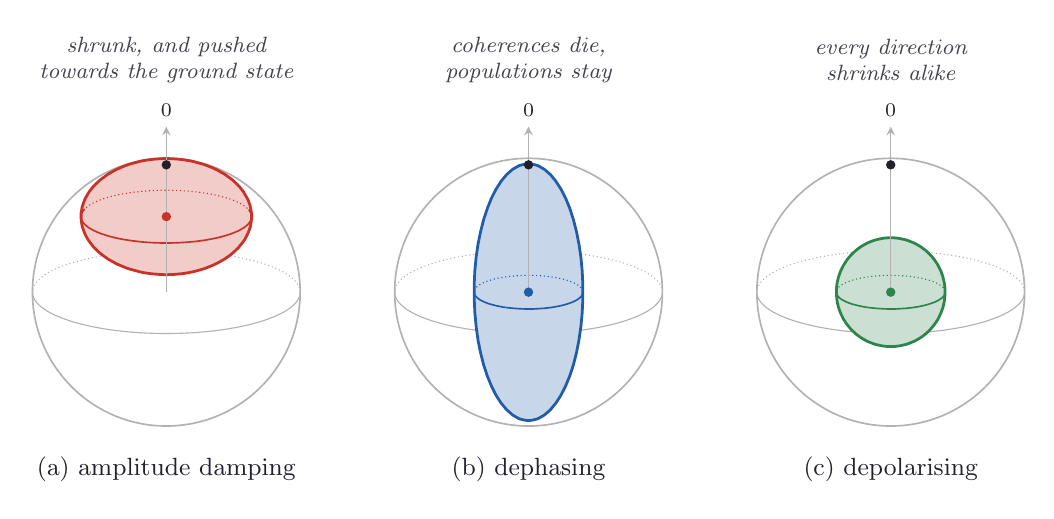
\begin{tikzpicture}[ink/.style={line width=0.9pt, ndInk}, faint/.style={line width=0.4pt, ndInk!35}, dashedink/.style={line width=0.5pt, ndInk!55, dash pattern=on 2.5pt off 2pt}, vec/.style={->, >=stealth, line width=1.2pt}, note/.style={font=\footnotesize\itshape, text=ndInk!85, align=center}, pointer/.style={->, >=stealth, line width=0.4pt, ndInk!60, shorten >=2pt, shorten <=1pt}, dot/.style={circle, fill=ndInk, inner sep=0pt, minimum size=3.4pt}, wash/.style={fill=ndSky, fill opacity=0.55}, every node/.style={text=ndInk}]
\definecolor{ndInk}{rgb}{0.13,0.13,0.18}
\definecolor{ndPaper}{rgb}{0.99,0.96,0.88}
\definecolor{ndSky}{rgb}{0.84,0.91,0.98}
\definecolor{ndRose}{rgb}{0.98,0.86,0.84}
\definecolor{ndBlue}{rgb}{0.13,0.36,0.66}
\definecolor{ndRed}{rgb}{0.78,0.20,0.16}
\definecolor{ndGold}{rgb}{0.88,0.62,0.10}
\definecolor{ndGreen}{rgb}{0.18,0.52,0.30}
\draw[faint, line width=0.6pt] (0.000,0.000) circle (1.700);
\draw[faint] (1.541,-0.222) -- (1.559,-0.209) -- (1.576,-0.197) -- (1.592,-0.184) -- (1.607,-0.171) -- (1.621,-0.158) -- (1.634,-0.145) -- (1.646,-0.132) -- (1.656,-0.118) -- (1.666,-0.105) -- (1.674,-0.091) -- (1.681,-0.078) -- (1.687,-0.064) -- (1.692,-0.050) -- (1.696,-0.037) -- (1.698,-0.023) -- (1.700,-0.009);
\draw[faint] (-1.700,-0.005) -- (-1.699,-0.018) -- (-1.697,-0.032) -- (-1.694,-0.046) -- (-1.689,-0.059) -- (-1.683,-0.073) -- (-1.677,-0.087) -- (-1.669,-0.100) -- (-1.660,-0.114) -- (-1.650,-0.127) -- (-1.638,-0.140) -- (-1.626,-0.154) -- (-1.612,-0.167) -- (-1.597,-0.180) -- (-1.582,-0.193) -- (-1.565,-0.205) -- (-1.547,-0.218) -- (-1.528,-0.230) -- (-1.508,-0.243) -- (-1.487,-0.255) -- (-1.465,-0.267) -- (-1.442,-0.278) -- (-1.418,-0.290) -- (-1.393,-0.301) -- (-1.367,-0.312) -- (-1.340,-0.323) -- (-1.312,-0.334) -- (-1.283,-0.345) -- (-1.253,-0.355) -- (-1.223,-0.365) -- (-1.192,-0.375) -- (-1.159,-0.384) -- (-1.126,-0.393) -- (-1.093,-0.402) -- (-1.058,-0.411) -- (-1.023,-0.420) -- (-0.987,-0.428) -- (-0.951,-0.436) -- (-0.913,-0.443) -- (-0.876,-0.450) -- (-0.837,-0.457) -- (-0.798,-0.464) -- (-0.759,-0.470) -- (-0.718,-0.476) -- (-0.678,-0.482) -- (-0.637,-0.487) -- (-0.595,-0.492) -- (-0.553,-0.497) -- (-0.511,-0.501) -- (-0.469,-0.505) -- (-0.426,-0.509) -- (-0.382,-0.512) -- (-0.339,-0.515) -- (-0.295,-0.517) -- (-0.251,-0.520) -- (-0.207,-0.521) -- (-0.163,-0.523) -- (-0.119,-0.524) -- (-0.074,-0.525) -- (-0.030,-0.525) -- (0.015,-0.525) -- (0.059,-0.525) -- (0.104,-0.524) -- (0.148,-0.523) -- (0.192,-0.522) -- (0.237,-0.520) -- (0.281,-0.518) -- (0.324,-0.516) -- (0.368,-0.513) -- (0.411,-0.510) -- (0.454,-0.506) -- (0.497,-0.502) -- (0.539,-0.498) -- (0.581,-0.494) -- (0.623,-0.489) -- (0.664,-0.484) -- (0.705,-0.478) -- (0.745,-0.472) -- (0.785,-0.466) -- (0.824,-0.459) -- (0.863,-0.453) -- (0.901,-0.446) -- (0.938,-0.438) -- (0.975,-0.430) -- (1.011,-0.422) -- (1.047,-0.414) -- (1.081,-0.405) -- (1.115,-0.396) -- (1.149,-0.387) -- (1.181,-0.378) -- (1.213,-0.368) -- (1.243,-0.358) -- (1.273,-0.348) -- (1.302,-0.338) -- (1.330,-0.327) -- (1.358,-0.316) -- (1.384,-0.305) -- (1.409,-0.294) -- (1.434,-0.282) -- (1.457,-0.271) -- (1.480,-0.259) -- (1.501,-0.247) -- (1.521,-0.234) -- (1.541,-0.222);
\draw[faint, densely dotted] (1.700,0.005) -- (1.699,0.018) -- (1.697,0.032) -- (1.694,0.046) -- (1.689,0.059) -- (1.683,0.073) -- (1.677,0.087) -- (1.669,0.100) -- (1.660,0.114) -- (1.650,0.127) -- (1.638,0.140) -- (1.626,0.154) -- (1.612,0.167) -- (1.597,0.180) -- (1.582,0.193) -- (1.565,0.205) -- (1.547,0.218) -- (1.528,0.230) -- (1.508,0.243) -- (1.487,0.255) -- (1.465,0.267) -- (1.442,0.278) -- (1.418,0.290) -- (1.393,0.301) -- (1.367,0.312) -- (1.340,0.323) -- (1.312,0.334) -- (1.283,0.345) -- (1.253,0.355) -- (1.223,0.365) -- (1.192,0.375) -- (1.159,0.384) -- (1.126,0.393) -- (1.093,0.402) -- (1.058,0.411) -- (1.023,0.420) -- (0.987,0.428) -- (0.951,0.436) -- (0.913,0.443) -- (0.876,0.450) -- (0.837,0.457) -- (0.798,0.464) -- (0.759,0.470) -- (0.718,0.476) -- (0.678,0.482) -- (0.637,0.487) -- (0.595,0.492) -- (0.553,0.497) -- (0.511,0.501) -- (0.469,0.505) -- (0.426,0.509) -- (0.382,0.512) -- (0.339,0.515) -- (0.295,0.517) -- (0.251,0.520) -- (0.207,0.521) -- (0.163,0.523) -- (0.119,0.524) -- (0.074,0.525) -- (0.030,0.525) -- (-0.015,0.525) -- (-0.059,0.525) -- (-0.104,0.524) -- (-0.148,0.523) -- (-0.192,0.522) -- (-0.237,0.520) -- (-0.281,0.518) -- (-0.324,0.516) -- (-0.368,0.513) -- (-0.411,0.510) -- (-0.454,0.506) -- (-0.497,0.502) -- (-0.539,0.498) -- (-0.581,0.494) -- (-0.623,0.489) -- (-0.664,0.484) -- (-0.705,0.478) -- (-0.745,0.472) -- (-0.785,0.466) -- (-0.824,0.459) -- (-0.863,0.453) -- (-0.901,0.446) -- (-0.938,0.438) -- (-0.975,0.430) -- (-1.011,0.422) -- (-1.047,0.414) -- (-1.081,0.405) -- (-1.115,0.396) -- (-1.149,0.387) -- (-1.181,0.378) -- (-1.213,0.368) -- (-1.243,0.358) -- (-1.273,0.348) -- (-1.302,0.338) -- (-1.330,0.327) -- (-1.358,0.316) -- (-1.384,0.305) -- (-1.409,0.294) -- (-1.434,0.282) -- (-1.457,0.271) -- (-1.480,0.259) -- (-1.501,0.247) -- (-1.521,0.234) -- (-1.541,0.222) -- (-1.559,0.209) -- (-1.576,0.197) -- (-1.592,0.184) -- (-1.607,0.171) -- (-1.621,0.158) -- (-1.634,0.145) -- (-1.646,0.132) -- (-1.656,0.118) -- (-1.666,0.105) -- (-1.674,0.091) -- (-1.681,0.078) -- (-1.687,0.064) -- (-1.692,0.050) -- (-1.696,0.037) -- (-1.698,0.023) -- (-1.700,0.009);
\filldraw[fill=ndRed!25, draw=ndRed, line width=1.0pt] (-1.080,0.901) -- (-1.067,0.830) -- (-1.042,0.761) -- (-1.028,0.727) -- (-0.991,0.662) -- (-0.967,0.629) -- (-0.920,0.569) -- (-0.862,0.513) -- (-0.830,0.485) -- (-0.764,0.437) -- (-0.727,0.413) -- (-0.656,0.373) -- (-0.614,0.352) -- (-0.541,0.321) -- (-0.498,0.304) -- (-0.450,0.289) -- (-0.383,0.271) -- (-0.338,0.259) -- (-0.289,0.248) -- (-0.236,0.240) -- (-0.181,0.233) -- (-0.147,0.230) -- (-0.101,0.226) -- (-0.053,0.223) -- (-0.005,0.222) -- (0.044,0.223) -- (0.092,0.225) -- (0.138,0.229) -- (0.170,0.232) -- (0.226,0.238) -- (0.279,0.247) -- (0.329,0.257) -- (0.375,0.268) -- (0.440,0.286) -- (0.489,0.301) -- (0.533,0.318) -- (0.606,0.348) -- (0.648,0.369) -- (0.719,0.408) -- (0.758,0.432) -- (0.823,0.480) -- (0.856,0.508) -- (0.914,0.563) -- (0.939,0.594) -- (0.988,0.655) -- (1.024,0.721) -- (1.040,0.755) -- (1.065,0.823) -- (1.078,0.894) -- (1.082,0.929) -- (1.082,1.000) -- (1.070,1.071) -- (1.062,1.106) -- (1.037,1.175) -- (0.999,1.241) -- (0.981,1.273) -- (0.933,1.335) -- (0.904,1.365) -- (0.847,1.420) -- (0.811,1.447) -- (0.747,1.494) -- (0.705,1.518) -- (0.636,1.557) -- (0.591,1.577) -- (0.520,1.606) -- (0.475,1.623) -- (0.424,1.637) -- (0.361,1.654) -- (0.314,1.666) -- (0.263,1.675) -- (0.209,1.683) -- (0.153,1.689) -- (0.124,1.691) -- (0.077,1.695) -- (0.029,1.696) -- (-0.020,1.697) -- (-0.068,1.695) -- (-0.115,1.692) -- (-0.141,1.690) -- (-0.198,1.684) -- (-0.253,1.677) -- (-0.304,1.668) -- (-0.352,1.657) -- (-0.413,1.640) -- (-0.465,1.626) -- (-0.512,1.610) -- (-0.582,1.581) -- (-0.628,1.561) -- (-0.667,1.540) -- (-0.739,1.499) -- (-0.774,1.474) -- (-0.841,1.425) -- (-0.897,1.371) -- (-0.928,1.341) -- (-0.976,1.280) -- (-0.997,1.247) -- (-1.034,1.181) -- (-1.059,1.113) -- (-1.069,1.078) -- (-1.082,1.007) -- (-1.082,0.936) -- cycle;
\draw[line width=0.6pt, ndRed] (-0.458,0.656) -- (-0.406,0.649) -- (-0.352,0.643) -- (-0.297,0.637) -- (-0.242,0.633) -- (-0.186,0.629) -- (-0.129,0.627) -- (-0.072,0.625) -- (-0.015,0.625) -- (0.042,0.625) -- (0.099,0.626) -- (0.156,0.628) -- (0.212,0.631) -- (0.268,0.635) -- (0.323,0.640) -- (0.377,0.645) -- (0.431,0.652) -- (0.482,0.659) -- (0.533,0.668) -- (0.582,0.677) -- (0.630,0.687) -- (0.675,0.697) -- (0.719,0.709) -- (0.761,0.721) -- (0.801,0.734) -- (0.838,0.747) -- (0.873,0.761) -- (0.906,0.775) -- (0.936,0.790) -- (0.964,0.806) -- (0.988,0.822) -- (1.010,0.838) -- (1.030,0.855) -- (1.046,0.872) -- (1.060,0.889) -- (1.070,0.906) -- (1.078,0.924) -- (1.082,0.942) -- (1.084,0.959) -- (1.082,0.977) -- (1.078,0.995) -- (1.071,1.012) -- (1.060,1.029) -- (1.047,1.047);
\draw[line width=0.6pt, ndRed] (-1.038,1.056) -- (-1.053,1.039) -- (-1.065,1.021) -- (-1.074,1.004) -- (-1.081,0.986) -- (-1.084,0.969) -- (-1.084,0.951) -- (-1.081,0.933) -- (-1.075,0.916) -- (-1.066,0.898) -- (-1.054,0.881) -- (-1.039,0.864) -- (-1.021,0.847) -- (-1.000,0.830) -- (-0.977,0.814) -- (-0.951,0.799) -- (-0.922,0.783) -- (-0.891,0.769) -- (-0.857,0.754) -- (-0.821,0.741) -- (-0.782,0.728) -- (-0.741,0.715) -- (-0.699,0.703) -- (-0.654,0.692) -- (-0.607,0.682) -- (-0.559,0.672) -- (-0.509,0.664) -- (-0.458,0.656);
\draw[line width=0.4pt, ndRed, densely dotted] (1.030,1.064) -- (1.011,1.080) -- (0.989,1.097) -- (0.964,1.112) -- (0.937,1.128) -- (0.907,1.143) -- (0.874,1.158) -- (0.839,1.172) -- (0.802,1.185) -- (0.762,1.198) -- (0.720,1.210) -- (0.676,1.221) -- (0.631,1.232) -- (0.583,1.242) -- (0.534,1.251) -- (0.484,1.259) -- (0.432,1.267) -- (0.379,1.273) -- (0.325,1.279) -- (0.270,1.284) -- (0.214,1.288) -- (0.158,1.291) -- (0.101,1.293) -- (0.044,1.294) -- (-0.014,1.294) -- (-0.071,1.294) -- (-0.128,1.292) -- (-0.184,1.290) -- (-0.240,1.286) -- (-0.296,1.282) -- (-0.350,1.276) -- (-0.404,1.270) -- (-0.457,1.263) -- (-0.508,1.255) -- (-0.558,1.247) -- (-0.606,1.237) -- (-0.653,1.227) -- (-0.697,1.216) -- (-0.740,1.204) -- (-0.781,1.192) -- (-0.820,1.179) -- (-0.856,1.165) -- (-0.890,1.151) -- (-0.921,1.136) -- (-0.950,1.121) -- (-0.976,1.105) -- (-1.000,1.089) -- (-1.020,1.072);
\draw[faint, ->, >=stealth] (0.000,0.000) -- (0.000,2.102) node[above, text=ndInk, font=\scriptsize] {$\ket0$};
\node[dot] at (0.000,1.617) {};
\node[dot, fill=ndRed] at (0.000,0.959) {};
\node[font=\small] at (0.000,-2.250) {(a) amplitude damping};
\draw[faint, line width=0.6pt] (4.600,0.000) circle (1.700);
\draw[faint] (6.141,-0.222) -- (6.159,-0.209) -- (6.176,-0.197) -- (6.192,-0.184) -- (6.207,-0.171) -- (6.221,-0.158) -- (6.234,-0.145) -- (6.246,-0.132) -- (6.256,-0.118) -- (6.266,-0.105) -- (6.274,-0.091) -- (6.281,-0.078) -- (6.287,-0.064) -- (6.292,-0.050) -- (6.296,-0.037) -- (6.298,-0.023) -- (6.300,-0.009);
\draw[faint] (2.900,-0.005) -- (2.901,-0.018) -- (2.903,-0.032) -- (2.906,-0.046) -- (2.911,-0.059) -- (2.917,-0.073) -- (2.923,-0.087) -- (2.931,-0.100) -- (2.940,-0.114) -- (2.950,-0.127) -- (2.962,-0.140) -- (2.974,-0.154) -- (2.988,-0.167) -- (3.003,-0.180) -- (3.018,-0.193) -- (3.035,-0.205) -- (3.053,-0.218) -- (3.072,-0.230) -- (3.092,-0.243) -- (3.113,-0.255) -- (3.135,-0.267) -- (3.158,-0.278) -- (3.182,-0.290) -- (3.207,-0.301) -- (3.233,-0.312) -- (3.260,-0.323) -- (3.288,-0.334) -- (3.317,-0.345) -- (3.347,-0.355) -- (3.377,-0.365) -- (3.408,-0.375) -- (3.441,-0.384) -- (3.474,-0.393) -- (3.507,-0.402) -- (3.542,-0.411) -- (3.577,-0.420) -- (3.613,-0.428) -- (3.649,-0.436) -- (3.687,-0.443) -- (3.724,-0.450) -- (3.763,-0.457) -- (3.802,-0.464) -- (3.841,-0.470) -- (3.882,-0.476) -- (3.922,-0.482) -- (3.963,-0.487) -- (4.005,-0.492) -- (4.047,-0.497) -- (4.089,-0.501) -- (4.131,-0.505) -- (4.174,-0.509) -- (4.218,-0.512) -- (4.261,-0.515) -- (4.305,-0.517) -- (4.349,-0.520) -- (4.393,-0.521) -- (4.437,-0.523) -- (4.481,-0.524) -- (4.526,-0.525) -- (4.570,-0.525) -- (4.615,-0.525) -- (4.659,-0.525) -- (4.704,-0.524) -- (4.748,-0.523) -- (4.792,-0.522) -- (4.837,-0.520) -- (4.881,-0.518) -- (4.924,-0.516) -- (4.968,-0.513) -- (5.011,-0.510) -- (5.054,-0.506) -- (5.097,-0.502) -- (5.139,-0.498) -- (5.181,-0.494) -- (5.223,-0.489) -- (5.264,-0.484) -- (5.305,-0.478) -- (5.345,-0.472) -- (5.385,-0.466) -- (5.424,-0.459) -- (5.463,-0.453) -- (5.501,-0.446) -- (5.538,-0.438) -- (5.575,-0.430) -- (5.611,-0.422) -- (5.647,-0.414) -- (5.681,-0.405) -- (5.715,-0.396) -- (5.749,-0.387) -- (5.781,-0.378) -- (5.813,-0.368) -- (5.843,-0.358) -- (5.873,-0.348) -- (5.902,-0.338) -- (5.930,-0.327) -- (5.958,-0.316) -- (5.984,-0.305) -- (6.009,-0.294) -- (6.034,-0.282) -- (6.057,-0.271) -- (6.080,-0.259) -- (6.101,-0.247) -- (6.121,-0.234) -- (6.141,-0.222);
\draw[faint, densely dotted] (6.300,0.005) -- (6.299,0.018) -- (6.297,0.032) -- (6.294,0.046) -- (6.289,0.059) -- (6.283,0.073) -- (6.277,0.087) -- (6.269,0.100) -- (6.260,0.114) -- (6.250,0.127) -- (6.238,0.140) -- (6.226,0.154) -- (6.212,0.167) -- (6.197,0.180) -- (6.182,0.193) -- (6.165,0.205) -- (6.147,0.218) -- (6.128,0.230) -- (6.108,0.243) -- (6.087,0.255) -- (6.065,0.267) -- (6.042,0.278) -- (6.018,0.290) -- (5.993,0.301) -- (5.967,0.312) -- (5.940,0.323) -- (5.912,0.334) -- (5.883,0.345) -- (5.853,0.355) -- (5.823,0.365) -- (5.792,0.375) -- (5.759,0.384) -- (5.726,0.393) -- (5.693,0.402) -- (5.658,0.411) -- (5.623,0.420) -- (5.587,0.428) -- (5.551,0.436) -- (5.513,0.443) -- (5.476,0.450) -- (5.437,0.457) -- (5.398,0.464) -- (5.359,0.470) -- (5.318,0.476) -- (5.278,0.482) -- (5.237,0.487) -- (5.195,0.492) -- (5.153,0.497) -- (5.111,0.501) -- (5.069,0.505) -- (5.026,0.509) -- (4.982,0.512) -- (4.939,0.515) -- (4.895,0.517) -- (4.851,0.520) -- (4.807,0.521) -- (4.763,0.523) -- (4.719,0.524) -- (4.674,0.525) -- (4.630,0.525) -- (4.585,0.525) -- (4.541,0.525) -- (4.496,0.524) -- (4.452,0.523) -- (4.408,0.522) -- (4.363,0.520) -- (4.319,0.518) -- (4.276,0.516) -- (4.232,0.513) -- (4.189,0.510) -- (4.146,0.506) -- (4.103,0.502) -- (4.061,0.498) -- (4.019,0.494) -- (3.977,0.489) -- (3.936,0.484) -- (3.895,0.478) -- (3.855,0.472) -- (3.815,0.466) -- (3.776,0.459) -- (3.737,0.453) -- (3.699,0.446) -- (3.662,0.438) -- (3.625,0.430) -- (3.589,0.422) -- (3.553,0.414) -- (3.519,0.405) -- (3.485,0.396) -- (3.451,0.387) -- (3.419,0.378) -- (3.387,0.368) -- (3.357,0.358) -- (3.327,0.348) -- (3.298,0.338) -- (3.270,0.327) -- (3.242,0.316) -- (3.216,0.305) -- (3.191,0.294) -- (3.166,0.282) -- (3.143,0.271) -- (3.120,0.259) -- (3.099,0.247) -- (3.079,0.234) -- (3.059,0.222) -- (3.041,0.209) -- (3.024,0.197) -- (3.008,0.184) -- (2.993,0.171) -- (2.979,0.158) -- (2.966,0.145) -- (2.954,0.132) -- (2.944,0.118) -- (2.934,0.105) -- (2.926,0.091) -- (2.919,0.078) -- (2.913,0.064) -- (2.908,0.050) -- (2.904,0.037) -- (2.902,0.023) -- (2.900,0.009);
\filldraw[fill=ndBlue!25, draw=ndBlue, line width=1.0pt] (3.910,0.095) -- (3.910,-0.080) -- (3.918,-0.254) -- (3.920,-0.276) -- (3.936,-0.447) -- (3.959,-0.612) -- (3.991,-0.770) -- (4.029,-0.920) -- (4.074,-1.058) -- (4.081,-1.075) -- (4.132,-1.200) -- (4.188,-1.310) -- (4.249,-1.405) -- (4.258,-1.416) -- (4.321,-1.492) -- (4.331,-1.501) -- (4.396,-1.558) -- (4.406,-1.565) -- (4.469,-1.601) -- (4.478,-1.605) -- (4.487,-1.609) -- (4.498,-1.612) -- (4.510,-1.616) -- (4.555,-1.626) -- (4.561,-1.627) -- (4.568,-1.628) -- (4.576,-1.629) -- (4.583,-1.630) -- (4.591,-1.630) -- (4.599,-1.630) -- (4.607,-1.630) -- (4.615,-1.630) -- (4.623,-1.629) -- (4.630,-1.628) -- (4.637,-1.627) -- (4.644,-1.626) -- (4.687,-1.616) -- (4.700,-1.613) -- (4.711,-1.610) -- (4.721,-1.606) -- (4.729,-1.602) -- (4.792,-1.566) -- (4.802,-1.559) -- (4.811,-1.553) -- (4.877,-1.494) -- (4.940,-1.418) -- (4.949,-1.407) -- (5.010,-1.312) -- (5.066,-1.202) -- (5.073,-1.187) -- (5.125,-1.061) -- (5.170,-0.923) -- (5.208,-0.774) -- (5.239,-0.616) -- (5.263,-0.451) -- (5.266,-0.429) -- (5.282,-0.258) -- (5.290,-0.084) -- (5.290,0.091) -- (5.282,0.265) -- (5.266,0.436) -- (5.242,0.602) -- (5.211,0.760) -- (5.206,0.780) -- (5.168,0.929) -- (5.123,1.067) -- (5.072,1.192) -- (5.015,1.303) -- (5.007,1.316) -- (4.947,1.410) -- (4.883,1.488) -- (4.874,1.497) -- (4.808,1.555) -- (4.799,1.561) -- (4.734,1.599) -- (4.727,1.603) -- (4.718,1.607) -- (4.708,1.611) -- (4.696,1.614) -- (4.683,1.617) -- (4.642,1.626) -- (4.635,1.628) -- (4.628,1.629) -- (4.620,1.630) -- (4.613,1.630) -- (4.605,1.630) -- (4.597,1.630) -- (4.589,1.630) -- (4.581,1.630) -- (4.574,1.629) -- (4.566,1.628) -- (4.559,1.627) -- (4.553,1.625) -- (4.506,1.615) -- (4.495,1.611) -- (4.484,1.608) -- (4.475,1.604) -- (4.467,1.600) -- (4.403,1.563) -- (4.393,1.556) -- (4.328,1.499) -- (4.319,1.490) -- (4.255,1.413) -- (4.247,1.401) -- (4.186,1.306) -- (4.130,1.195) -- (4.079,1.070) -- (4.034,0.933) -- (4.028,0.914) -- (3.990,0.764) -- (3.958,0.606) -- (3.934,0.440) -- (3.918,0.269) -- cycle;
\draw[line width=0.6pt, ndBlue] (4.308,-0.194) -- (4.341,-0.198) -- (4.376,-0.202) -- (4.410,-0.205) -- (4.446,-0.208) -- (4.481,-0.210) -- (4.518,-0.212) -- (4.554,-0.213) -- (4.590,-0.214) -- (4.627,-0.213) -- (4.663,-0.213) -- (4.700,-0.211) -- (4.735,-0.209) -- (4.771,-0.207) -- (4.806,-0.204) -- (4.841,-0.200) -- (4.875,-0.196) -- (4.908,-0.191) -- (4.940,-0.186) -- (4.971,-0.180) -- (5.001,-0.174) -- (5.031,-0.167) -- (5.058,-0.160) -- (5.085,-0.152) -- (5.110,-0.144) -- (5.134,-0.135) -- (5.157,-0.127) -- (5.178,-0.117) -- (5.197,-0.108) -- (5.214,-0.098) -- (5.230,-0.088) -- (5.244,-0.077) -- (5.257,-0.067) -- (5.267,-0.056) -- (5.276,-0.045) -- (5.282,-0.034) -- (5.287,-0.023) -- (5.290,-0.011) -- (5.291,-0.000);
\draw[line width=0.6pt, ndBlue] (3.909,-0.005) -- (3.911,-0.017) -- (3.915,-0.028) -- (3.921,-0.039) -- (3.928,-0.050) -- (3.938,-0.061) -- (3.949,-0.072) -- (3.962,-0.082) -- (3.977,-0.093) -- (3.994,-0.103) -- (4.012,-0.112) -- (4.032,-0.122) -- (4.054,-0.131) -- (4.077,-0.140) -- (4.101,-0.148) -- (4.127,-0.156) -- (4.155,-0.163) -- (4.183,-0.170) -- (4.213,-0.177) -- (4.244,-0.183) -- (4.275,-0.189) -- (4.308,-0.194);
\draw[line width=0.4pt, ndBlue, densely dotted] (5.290,0.011) -- (5.287,0.022) -- (5.283,0.034) -- (5.276,0.045) -- (5.267,0.056) -- (5.257,0.066) -- (5.245,0.077) -- (5.231,0.087) -- (5.215,0.098) -- (5.197,0.107) -- (5.178,0.117) -- (5.157,0.126) -- (5.135,0.135) -- (5.111,0.144) -- (5.086,0.152) -- (5.059,0.160) -- (5.031,0.167) -- (5.002,0.174) -- (4.972,0.180) -- (4.941,0.186) -- (4.909,0.191) -- (4.875,0.196) -- (4.842,0.200) -- (4.807,0.204) -- (4.772,0.207) -- (4.736,0.209) -- (4.701,0.211) -- (4.664,0.213) -- (4.628,0.213) -- (4.591,0.214) -- (4.555,0.213) -- (4.519,0.212) -- (4.482,0.210) -- (4.447,0.208) -- (4.411,0.205) -- (4.377,0.202) -- (4.342,0.198) -- (4.309,0.194) -- (4.276,0.189) -- (4.244,0.183) -- (4.214,0.177) -- (4.184,0.171) -- (4.155,0.164) -- (4.128,0.156) -- (4.102,0.148) -- (4.077,0.140) -- (4.054,0.131) -- (4.033,0.122) -- (4.013,0.113) -- (3.994,0.103) -- (3.977,0.093) -- (3.963,0.083) -- (3.949,0.072) -- (3.938,0.061) -- (3.928,0.050) -- (3.921,0.039) -- (3.915,0.028) -- (3.911,0.017) -- (3.909,0.006);
\draw[faint, ->, >=stealth] (4.600,0.000) -- (4.600,2.102) node[above, text=ndInk, font=\scriptsize] {$\ket0$};
\node[dot] at (4.600,1.617) {};
\node[dot, fill=ndBlue] at (4.600,0.000) {};
\node[font=\small] at (4.600,-2.250) {(b) dephasing};
\draw[faint, line width=0.6pt] (9.200,0.000) circle (1.700);
\draw[faint] (10.741,-0.222) -- (10.759,-0.209) -- (10.776,-0.197) -- (10.792,-0.184) -- (10.807,-0.171) -- (10.821,-0.158) -- (10.834,-0.145) -- (10.846,-0.132) -- (10.856,-0.118) -- (10.866,-0.105) -- (10.874,-0.091) -- (10.881,-0.078) -- (10.887,-0.064) -- (10.892,-0.050) -- (10.896,-0.037) -- (10.898,-0.023) -- (10.900,-0.009);
\draw[faint] (7.500,-0.005) -- (7.501,-0.018) -- (7.503,-0.032) -- (7.506,-0.046) -- (7.511,-0.059) -- (7.517,-0.073) -- (7.523,-0.087) -- (7.531,-0.100) -- (7.540,-0.114) -- (7.550,-0.127) -- (7.562,-0.140) -- (7.574,-0.154) -- (7.588,-0.167) -- (7.603,-0.180) -- (7.618,-0.193) -- (7.635,-0.205) -- (7.653,-0.218) -- (7.672,-0.230) -- (7.692,-0.243) -- (7.713,-0.255) -- (7.735,-0.267) -- (7.758,-0.278) -- (7.782,-0.290) -- (7.807,-0.301) -- (7.833,-0.312) -- (7.860,-0.323) -- (7.888,-0.334) -- (7.917,-0.345) -- (7.947,-0.355) -- (7.977,-0.365) -- (8.008,-0.375) -- (8.041,-0.384) -- (8.074,-0.393) -- (8.107,-0.402) -- (8.142,-0.411) -- (8.177,-0.420) -- (8.213,-0.428) -- (8.249,-0.436) -- (8.287,-0.443) -- (8.324,-0.450) -- (8.363,-0.457) -- (8.402,-0.464) -- (8.441,-0.470) -- (8.482,-0.476) -- (8.522,-0.482) -- (8.563,-0.487) -- (8.605,-0.492) -- (8.647,-0.497) -- (8.689,-0.501) -- (8.731,-0.505) -- (8.774,-0.509) -- (8.818,-0.512) -- (8.861,-0.515) -- (8.905,-0.517) -- (8.949,-0.520) -- (8.993,-0.521) -- (9.037,-0.523) -- (9.081,-0.524) -- (9.126,-0.525) -- (9.170,-0.525) -- (9.215,-0.525) -- (9.259,-0.525) -- (9.304,-0.524) -- (9.348,-0.523) -- (9.392,-0.522) -- (9.437,-0.520) -- (9.481,-0.518) -- (9.524,-0.516) -- (9.568,-0.513) -- (9.611,-0.510) -- (9.654,-0.506) -- (9.697,-0.502) -- (9.739,-0.498) -- (9.781,-0.494) -- (9.823,-0.489) -- (9.864,-0.484) -- (9.905,-0.478) -- (9.945,-0.472) -- (9.985,-0.466) -- (10.024,-0.459) -- (10.063,-0.453) -- (10.101,-0.446) -- (10.138,-0.438) -- (10.175,-0.430) -- (10.211,-0.422) -- (10.247,-0.414) -- (10.281,-0.405) -- (10.315,-0.396) -- (10.349,-0.387) -- (10.381,-0.378) -- (10.413,-0.368) -- (10.443,-0.358) -- (10.473,-0.348) -- (10.502,-0.338) -- (10.530,-0.327) -- (10.558,-0.316) -- (10.584,-0.305) -- (10.609,-0.294) -- (10.634,-0.282) -- (10.657,-0.271) -- (10.680,-0.259) -- (10.701,-0.247) -- (10.721,-0.234) -- (10.741,-0.222);
\draw[faint, densely dotted] (10.900,0.005) -- (10.899,0.018) -- (10.897,0.032) -- (10.894,0.046) -- (10.889,0.059) -- (10.883,0.073) -- (10.877,0.087) -- (10.869,0.100) -- (10.860,0.114) -- (10.850,0.127) -- (10.838,0.140) -- (10.826,0.154) -- (10.812,0.167) -- (10.797,0.180) -- (10.782,0.193) -- (10.765,0.205) -- (10.747,0.218) -- (10.728,0.230) -- (10.708,0.243) -- (10.687,0.255) -- (10.665,0.267) -- (10.642,0.278) -- (10.618,0.290) -- (10.593,0.301) -- (10.567,0.312) -- (10.540,0.323) -- (10.512,0.334) -- (10.483,0.345) -- (10.453,0.355) -- (10.423,0.365) -- (10.392,0.375) -- (10.359,0.384) -- (10.326,0.393) -- (10.293,0.402) -- (10.258,0.411) -- (10.223,0.420) -- (10.187,0.428) -- (10.151,0.436) -- (10.113,0.443) -- (10.076,0.450) -- (10.037,0.457) -- (9.998,0.464) -- (9.959,0.470) -- (9.918,0.476) -- (9.878,0.482) -- (9.837,0.487) -- (9.795,0.492) -- (9.753,0.497) -- (9.711,0.501) -- (9.669,0.505) -- (9.626,0.509) -- (9.582,0.512) -- (9.539,0.515) -- (9.495,0.517) -- (9.451,0.520) -- (9.407,0.521) -- (9.363,0.523) -- (9.319,0.524) -- (9.274,0.525) -- (9.230,0.525) -- (9.185,0.525) -- (9.141,0.525) -- (9.096,0.524) -- (9.052,0.523) -- (9.008,0.522) -- (8.963,0.520) -- (8.919,0.518) -- (8.876,0.516) -- (8.832,0.513) -- (8.789,0.510) -- (8.746,0.506) -- (8.703,0.502) -- (8.661,0.498) -- (8.619,0.494) -- (8.577,0.489) -- (8.536,0.484) -- (8.495,0.478) -- (8.455,0.472) -- (8.415,0.466) -- (8.376,0.459) -- (8.337,0.453) -- (8.299,0.446) -- (8.262,0.438) -- (8.225,0.430) -- (8.189,0.422) -- (8.153,0.414) -- (8.119,0.405) -- (8.085,0.396) -- (8.051,0.387) -- (8.019,0.378) -- (7.987,0.368) -- (7.957,0.358) -- (7.927,0.348) -- (7.898,0.338) -- (7.870,0.327) -- (7.842,0.316) -- (7.816,0.305) -- (7.791,0.294) -- (7.766,0.282) -- (7.743,0.271) -- (7.720,0.259) -- (7.699,0.247) -- (7.679,0.234) -- (7.659,0.222) -- (7.641,0.209) -- (7.624,0.197) -- (7.608,0.184) -- (7.593,0.171) -- (7.579,0.158) -- (7.566,0.145) -- (7.554,0.132) -- (7.544,0.118) -- (7.534,0.105) -- (7.526,0.091) -- (7.519,0.078) -- (7.513,0.064) -- (7.508,0.050) -- (7.504,0.037) -- (7.502,0.023) -- (7.500,0.009);
\filldraw[fill=ndGreen!25, draw=ndGreen, line width=1.0pt] (8.512,-0.050) -- (8.520,-0.121) -- (8.536,-0.190) -- (8.559,-0.257) -- (8.568,-0.278) -- (8.599,-0.341) -- (8.637,-0.400) -- (8.651,-0.418) -- (8.694,-0.471) -- (8.744,-0.518) -- (8.760,-0.533) -- (8.813,-0.572) -- (8.832,-0.585) -- (8.887,-0.616) -- (8.906,-0.626) -- (8.929,-0.635) -- (8.980,-0.655) -- (9.001,-0.662) -- (9.025,-0.668) -- (9.067,-0.677) -- (9.086,-0.681) -- (9.107,-0.685) -- (9.129,-0.687) -- (9.151,-0.689) -- (9.174,-0.691) -- (9.198,-0.691) -- (9.221,-0.691) -- (9.244,-0.690) -- (9.267,-0.688) -- (9.289,-0.685) -- (9.310,-0.682) -- (9.330,-0.678) -- (9.371,-0.669) -- (9.395,-0.663) -- (9.416,-0.656) -- (9.436,-0.649) -- (9.489,-0.627) -- (9.510,-0.618) -- (9.564,-0.587) -- (9.584,-0.575) -- (9.636,-0.536) -- (9.654,-0.521) -- (9.703,-0.474) -- (9.717,-0.457) -- (9.761,-0.403) -- (9.799,-0.345) -- (9.830,-0.282) -- (9.839,-0.261) -- (9.863,-0.194) -- (9.879,-0.125) -- (9.882,-0.103) -- (9.890,-0.032) -- (9.890,0.039) -- (9.882,0.110) -- (9.877,0.132) -- (9.861,0.201) -- (9.837,0.268) -- (9.806,0.331) -- (9.795,0.351) -- (9.757,0.409) -- (9.713,0.463) -- (9.697,0.479) -- (9.649,0.526) -- (9.630,0.540) -- (9.578,0.579) -- (9.557,0.591) -- (9.504,0.621) -- (9.483,0.630) -- (9.430,0.651) -- (9.410,0.658) -- (9.388,0.665) -- (9.363,0.671) -- (9.324,0.679) -- (9.304,0.683) -- (9.282,0.686) -- (9.260,0.689) -- (9.237,0.690) -- (9.214,0.691) -- (9.191,0.691) -- (9.167,0.690) -- (9.144,0.689) -- (9.122,0.687) -- (9.100,0.684) -- (9.080,0.680) -- (9.042,0.672) -- (9.017,0.666) -- (8.994,0.660) -- (8.974,0.653) -- (8.922,0.632) -- (8.900,0.623) -- (8.881,0.612) -- (8.826,0.581) -- (8.808,0.568) -- (8.755,0.528) -- (8.706,0.482) -- (8.690,0.466) -- (8.646,0.413) -- (8.634,0.394) -- (8.596,0.335) -- (8.565,0.272) -- (8.541,0.205) -- (8.534,0.183) -- (8.518,0.114) -- (8.510,0.043) -- (8.510,-0.028) -- cycle;
\draw[line width=0.6pt, ndGreen] (8.908,-0.194) -- (8.941,-0.198) -- (8.976,-0.202) -- (9.010,-0.205) -- (9.046,-0.208) -- (9.081,-0.210) -- (9.118,-0.212) -- (9.154,-0.213) -- (9.190,-0.214) -- (9.227,-0.213) -- (9.263,-0.213) -- (9.300,-0.211) -- (9.335,-0.209) -- (9.371,-0.207) -- (9.406,-0.204) -- (9.441,-0.200) -- (9.475,-0.196) -- (9.508,-0.191) -- (9.540,-0.186) -- (9.571,-0.180) -- (9.601,-0.174) -- (9.631,-0.167) -- (9.658,-0.160) -- (9.685,-0.152) -- (9.710,-0.144) -- (9.734,-0.135) -- (9.757,-0.127) -- (9.778,-0.117) -- (9.797,-0.108) -- (9.814,-0.098) -- (9.830,-0.088) -- (9.844,-0.077) -- (9.857,-0.067) -- (9.867,-0.056) -- (9.876,-0.045) -- (9.882,-0.034) -- (9.887,-0.023) -- (9.890,-0.011) -- (9.891,-0.000);
\draw[line width=0.6pt, ndGreen] (8.509,-0.005) -- (8.511,-0.017) -- (8.515,-0.028) -- (8.521,-0.039) -- (8.528,-0.050) -- (8.538,-0.061) -- (8.549,-0.072) -- (8.562,-0.082) -- (8.577,-0.093) -- (8.594,-0.103) -- (8.612,-0.112) -- (8.632,-0.122) -- (8.654,-0.131) -- (8.677,-0.140) -- (8.701,-0.148) -- (8.727,-0.156) -- (8.755,-0.163) -- (8.783,-0.170) -- (8.813,-0.177) -- (8.844,-0.183) -- (8.875,-0.189) -- (8.908,-0.194);
\draw[line width=0.4pt, ndGreen, densely dotted] (9.890,0.011) -- (9.887,0.022) -- (9.883,0.034) -- (9.876,0.045) -- (9.867,0.056) -- (9.857,0.066) -- (9.845,0.077) -- (9.831,0.087) -- (9.815,0.098) -- (9.797,0.107) -- (9.778,0.117) -- (9.757,0.126) -- (9.735,0.135) -- (9.711,0.144) -- (9.686,0.152) -- (9.659,0.160) -- (9.631,0.167) -- (9.602,0.174) -- (9.572,0.180) -- (9.541,0.186) -- (9.509,0.191) -- (9.475,0.196) -- (9.442,0.200) -- (9.407,0.204) -- (9.372,0.207) -- (9.336,0.209) -- (9.301,0.211) -- (9.264,0.213) -- (9.228,0.213) -- (9.191,0.214) -- (9.155,0.213) -- (9.119,0.212) -- (9.082,0.210) -- (9.047,0.208) -- (9.011,0.205) -- (8.977,0.202) -- (8.942,0.198) -- (8.909,0.194) -- (8.876,0.189) -- (8.844,0.183) -- (8.814,0.177) -- (8.784,0.171) -- (8.755,0.164) -- (8.728,0.156) -- (8.702,0.148) -- (8.677,0.140) -- (8.654,0.131) -- (8.633,0.122) -- (8.613,0.113) -- (8.594,0.103) -- (8.577,0.093) -- (8.563,0.083) -- (8.549,0.072) -- (8.538,0.061) -- (8.528,0.050) -- (8.521,0.039) -- (8.515,0.028) -- (8.511,0.017) -- (8.509,0.006);
\draw[faint, ->, >=stealth] (9.200,0.000) -- (9.200,2.102) node[above, text=ndInk, font=\scriptsize] {$\ket0$};
\node[dot] at (9.200,1.617) {};
\node[dot, fill=ndGreen] at (9.200,0.000) {};
\node[font=\small] at (9.200,-2.250) {(c) depolarising};
\node[note] at (0,2.95) {shrunk, and pushed\\ towards the ground state};
\node[note] at (4.6,2.95) {coherences die,\\ populations stay};
\node[note] at (9.2,2.95) {every direction\\ shrinks alike};
\end{tikzpicture}
}
\caption{The image of the Bloch ball (shaded) after time $t$ with $\gamma t=0.9$ under (a) amplitude damping, (b) dephasing and (c) depolarising noise. The semi-axes are $(\ee^{-\gamma t/2},\ee^{-\gamma t/2},\ee^{-\gamma t})$ with centre $(0,0,1-\ee^{-\gamma t})$, $(\ee^{-\gamma t},\ee^{-\gamma t},1)$, and $\ee^{-\gamma t}$ in all directions, respectively. Generated by \texttt{code/ch03\_channels.py}.}\label{fig:ch03:channels}
\end{figure}}
\ona{\endgraf\medskip\noindent\textit{Reading the figure.} In each panel the grey sphere stands for all states before the noise acts, and the shaded body for the same states after the noise has acted for a fixed time. The dark dot on top is the ground state $\ket0$, and the coloured dot the centre of the image.\endgraf\smallskip\noindent\textit{Why it matters.} These are the three standard noise models of quantum computing. Amplitude damping is energy loss, for instance spontaneous emission of a photon; dephasing comes from fluctuating energy levels, for instance a noisy magnetic field; depolarising noise is the isotropic, ``worst-case'' model used by default in simulations of quantum error-correcting codes. The three leave different fingerprints on the shape of the image, and that is precisely what makes them distinguishable in experiments: preparing several initial states, letting them evolve, and measuring $\sigx,\sigy,\sigz$ reveals the shape, and hence the noise. Doing this systematically is the identification problem of \Chaps~\ref{C.StateSpace}--\ref{C.SampleComplexity} and~\ref{C.AlgTomography}.}
\onp{\begin{center}\resizebox{\linewidth}{!}{% Generated by code/needham.py -- do not edit by hand.
\definecolor{qocA}{rgb}{0.00,0.45,0.70}
\definecolor{qocB}{rgb}{0.90,0.60,0.00}
\definecolor{qocC}{rgb}{0.00,0.62,0.45}
\definecolor{qocD}{rgb}{0.80,0.40,0.00}
\definecolor{qocE}{rgb}{0.80,0.60,0.70}
\definecolor{qocF}{rgb}{0.35,0.70,0.90}
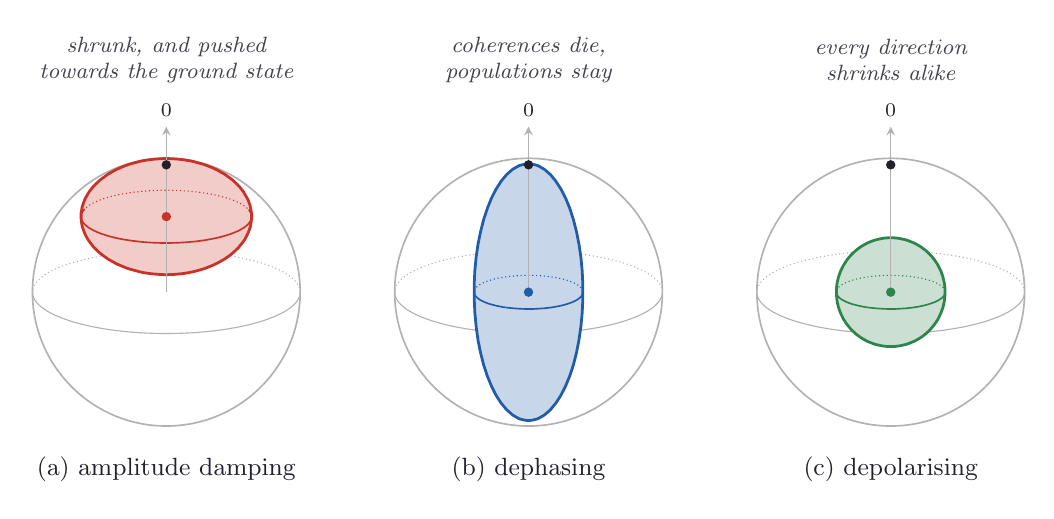
\begin{tikzpicture}[ink/.style={line width=0.9pt, ndInk}, faint/.style={line width=0.4pt, ndInk!35}, dashedink/.style={line width=0.5pt, ndInk!55, dash pattern=on 2.5pt off 2pt}, vec/.style={->, >=stealth, line width=1.2pt}, note/.style={font=\footnotesize\itshape, text=ndInk!85, align=center}, pointer/.style={->, >=stealth, line width=0.4pt, ndInk!60, shorten >=2pt, shorten <=1pt}, dot/.style={circle, fill=ndInk, inner sep=0pt, minimum size=3.4pt}, wash/.style={fill=ndSky, fill opacity=0.55}, every node/.style={text=ndInk}]
\definecolor{ndInk}{rgb}{0.13,0.13,0.18}
\definecolor{ndPaper}{rgb}{0.99,0.96,0.88}
\definecolor{ndSky}{rgb}{0.84,0.91,0.98}
\definecolor{ndRose}{rgb}{0.98,0.86,0.84}
\definecolor{ndBlue}{rgb}{0.13,0.36,0.66}
\definecolor{ndRed}{rgb}{0.78,0.20,0.16}
\definecolor{ndGold}{rgb}{0.88,0.62,0.10}
\definecolor{ndGreen}{rgb}{0.18,0.52,0.30}
\draw[faint, line width=0.6pt] (0.000,0.000) circle (1.700);
\draw[faint] (1.541,-0.222) -- (1.559,-0.209) -- (1.576,-0.197) -- (1.592,-0.184) -- (1.607,-0.171) -- (1.621,-0.158) -- (1.634,-0.145) -- (1.646,-0.132) -- (1.656,-0.118) -- (1.666,-0.105) -- (1.674,-0.091) -- (1.681,-0.078) -- (1.687,-0.064) -- (1.692,-0.050) -- (1.696,-0.037) -- (1.698,-0.023) -- (1.700,-0.009);
\draw[faint] (-1.700,-0.005) -- (-1.699,-0.018) -- (-1.697,-0.032) -- (-1.694,-0.046) -- (-1.689,-0.059) -- (-1.683,-0.073) -- (-1.677,-0.087) -- (-1.669,-0.100) -- (-1.660,-0.114) -- (-1.650,-0.127) -- (-1.638,-0.140) -- (-1.626,-0.154) -- (-1.612,-0.167) -- (-1.597,-0.180) -- (-1.582,-0.193) -- (-1.565,-0.205) -- (-1.547,-0.218) -- (-1.528,-0.230) -- (-1.508,-0.243) -- (-1.487,-0.255) -- (-1.465,-0.267) -- (-1.442,-0.278) -- (-1.418,-0.290) -- (-1.393,-0.301) -- (-1.367,-0.312) -- (-1.340,-0.323) -- (-1.312,-0.334) -- (-1.283,-0.345) -- (-1.253,-0.355) -- (-1.223,-0.365) -- (-1.192,-0.375) -- (-1.159,-0.384) -- (-1.126,-0.393) -- (-1.093,-0.402) -- (-1.058,-0.411) -- (-1.023,-0.420) -- (-0.987,-0.428) -- (-0.951,-0.436) -- (-0.913,-0.443) -- (-0.876,-0.450) -- (-0.837,-0.457) -- (-0.798,-0.464) -- (-0.759,-0.470) -- (-0.718,-0.476) -- (-0.678,-0.482) -- (-0.637,-0.487) -- (-0.595,-0.492) -- (-0.553,-0.497) -- (-0.511,-0.501) -- (-0.469,-0.505) -- (-0.426,-0.509) -- (-0.382,-0.512) -- (-0.339,-0.515) -- (-0.295,-0.517) -- (-0.251,-0.520) -- (-0.207,-0.521) -- (-0.163,-0.523) -- (-0.119,-0.524) -- (-0.074,-0.525) -- (-0.030,-0.525) -- (0.015,-0.525) -- (0.059,-0.525) -- (0.104,-0.524) -- (0.148,-0.523) -- (0.192,-0.522) -- (0.237,-0.520) -- (0.281,-0.518) -- (0.324,-0.516) -- (0.368,-0.513) -- (0.411,-0.510) -- (0.454,-0.506) -- (0.497,-0.502) -- (0.539,-0.498) -- (0.581,-0.494) -- (0.623,-0.489) -- (0.664,-0.484) -- (0.705,-0.478) -- (0.745,-0.472) -- (0.785,-0.466) -- (0.824,-0.459) -- (0.863,-0.453) -- (0.901,-0.446) -- (0.938,-0.438) -- (0.975,-0.430) -- (1.011,-0.422) -- (1.047,-0.414) -- (1.081,-0.405) -- (1.115,-0.396) -- (1.149,-0.387) -- (1.181,-0.378) -- (1.213,-0.368) -- (1.243,-0.358) -- (1.273,-0.348) -- (1.302,-0.338) -- (1.330,-0.327) -- (1.358,-0.316) -- (1.384,-0.305) -- (1.409,-0.294) -- (1.434,-0.282) -- (1.457,-0.271) -- (1.480,-0.259) -- (1.501,-0.247) -- (1.521,-0.234) -- (1.541,-0.222);
\draw[faint, densely dotted] (1.700,0.005) -- (1.699,0.018) -- (1.697,0.032) -- (1.694,0.046) -- (1.689,0.059) -- (1.683,0.073) -- (1.677,0.087) -- (1.669,0.100) -- (1.660,0.114) -- (1.650,0.127) -- (1.638,0.140) -- (1.626,0.154) -- (1.612,0.167) -- (1.597,0.180) -- (1.582,0.193) -- (1.565,0.205) -- (1.547,0.218) -- (1.528,0.230) -- (1.508,0.243) -- (1.487,0.255) -- (1.465,0.267) -- (1.442,0.278) -- (1.418,0.290) -- (1.393,0.301) -- (1.367,0.312) -- (1.340,0.323) -- (1.312,0.334) -- (1.283,0.345) -- (1.253,0.355) -- (1.223,0.365) -- (1.192,0.375) -- (1.159,0.384) -- (1.126,0.393) -- (1.093,0.402) -- (1.058,0.411) -- (1.023,0.420) -- (0.987,0.428) -- (0.951,0.436) -- (0.913,0.443) -- (0.876,0.450) -- (0.837,0.457) -- (0.798,0.464) -- (0.759,0.470) -- (0.718,0.476) -- (0.678,0.482) -- (0.637,0.487) -- (0.595,0.492) -- (0.553,0.497) -- (0.511,0.501) -- (0.469,0.505) -- (0.426,0.509) -- (0.382,0.512) -- (0.339,0.515) -- (0.295,0.517) -- (0.251,0.520) -- (0.207,0.521) -- (0.163,0.523) -- (0.119,0.524) -- (0.074,0.525) -- (0.030,0.525) -- (-0.015,0.525) -- (-0.059,0.525) -- (-0.104,0.524) -- (-0.148,0.523) -- (-0.192,0.522) -- (-0.237,0.520) -- (-0.281,0.518) -- (-0.324,0.516) -- (-0.368,0.513) -- (-0.411,0.510) -- (-0.454,0.506) -- (-0.497,0.502) -- (-0.539,0.498) -- (-0.581,0.494) -- (-0.623,0.489) -- (-0.664,0.484) -- (-0.705,0.478) -- (-0.745,0.472) -- (-0.785,0.466) -- (-0.824,0.459) -- (-0.863,0.453) -- (-0.901,0.446) -- (-0.938,0.438) -- (-0.975,0.430) -- (-1.011,0.422) -- (-1.047,0.414) -- (-1.081,0.405) -- (-1.115,0.396) -- (-1.149,0.387) -- (-1.181,0.378) -- (-1.213,0.368) -- (-1.243,0.358) -- (-1.273,0.348) -- (-1.302,0.338) -- (-1.330,0.327) -- (-1.358,0.316) -- (-1.384,0.305) -- (-1.409,0.294) -- (-1.434,0.282) -- (-1.457,0.271) -- (-1.480,0.259) -- (-1.501,0.247) -- (-1.521,0.234) -- (-1.541,0.222) -- (-1.559,0.209) -- (-1.576,0.197) -- (-1.592,0.184) -- (-1.607,0.171) -- (-1.621,0.158) -- (-1.634,0.145) -- (-1.646,0.132) -- (-1.656,0.118) -- (-1.666,0.105) -- (-1.674,0.091) -- (-1.681,0.078) -- (-1.687,0.064) -- (-1.692,0.050) -- (-1.696,0.037) -- (-1.698,0.023) -- (-1.700,0.009);
\filldraw[fill=ndRed!25, draw=ndRed, line width=1.0pt] (-1.080,0.901) -- (-1.067,0.830) -- (-1.042,0.761) -- (-1.028,0.727) -- (-0.991,0.662) -- (-0.967,0.629) -- (-0.920,0.569) -- (-0.862,0.513) -- (-0.830,0.485) -- (-0.764,0.437) -- (-0.727,0.413) -- (-0.656,0.373) -- (-0.614,0.352) -- (-0.541,0.321) -- (-0.498,0.304) -- (-0.450,0.289) -- (-0.383,0.271) -- (-0.338,0.259) -- (-0.289,0.248) -- (-0.236,0.240) -- (-0.181,0.233) -- (-0.147,0.230) -- (-0.101,0.226) -- (-0.053,0.223) -- (-0.005,0.222) -- (0.044,0.223) -- (0.092,0.225) -- (0.138,0.229) -- (0.170,0.232) -- (0.226,0.238) -- (0.279,0.247) -- (0.329,0.257) -- (0.375,0.268) -- (0.440,0.286) -- (0.489,0.301) -- (0.533,0.318) -- (0.606,0.348) -- (0.648,0.369) -- (0.719,0.408) -- (0.758,0.432) -- (0.823,0.480) -- (0.856,0.508) -- (0.914,0.563) -- (0.939,0.594) -- (0.988,0.655) -- (1.024,0.721) -- (1.040,0.755) -- (1.065,0.823) -- (1.078,0.894) -- (1.082,0.929) -- (1.082,1.000) -- (1.070,1.071) -- (1.062,1.106) -- (1.037,1.175) -- (0.999,1.241) -- (0.981,1.273) -- (0.933,1.335) -- (0.904,1.365) -- (0.847,1.420) -- (0.811,1.447) -- (0.747,1.494) -- (0.705,1.518) -- (0.636,1.557) -- (0.591,1.577) -- (0.520,1.606) -- (0.475,1.623) -- (0.424,1.637) -- (0.361,1.654) -- (0.314,1.666) -- (0.263,1.675) -- (0.209,1.683) -- (0.153,1.689) -- (0.124,1.691) -- (0.077,1.695) -- (0.029,1.696) -- (-0.020,1.697) -- (-0.068,1.695) -- (-0.115,1.692) -- (-0.141,1.690) -- (-0.198,1.684) -- (-0.253,1.677) -- (-0.304,1.668) -- (-0.352,1.657) -- (-0.413,1.640) -- (-0.465,1.626) -- (-0.512,1.610) -- (-0.582,1.581) -- (-0.628,1.561) -- (-0.667,1.540) -- (-0.739,1.499) -- (-0.774,1.474) -- (-0.841,1.425) -- (-0.897,1.371) -- (-0.928,1.341) -- (-0.976,1.280) -- (-0.997,1.247) -- (-1.034,1.181) -- (-1.059,1.113) -- (-1.069,1.078) -- (-1.082,1.007) -- (-1.082,0.936) -- cycle;
\draw[line width=0.6pt, ndRed] (-0.458,0.656) -- (-0.406,0.649) -- (-0.352,0.643) -- (-0.297,0.637) -- (-0.242,0.633) -- (-0.186,0.629) -- (-0.129,0.627) -- (-0.072,0.625) -- (-0.015,0.625) -- (0.042,0.625) -- (0.099,0.626) -- (0.156,0.628) -- (0.212,0.631) -- (0.268,0.635) -- (0.323,0.640) -- (0.377,0.645) -- (0.431,0.652) -- (0.482,0.659) -- (0.533,0.668) -- (0.582,0.677) -- (0.630,0.687) -- (0.675,0.697) -- (0.719,0.709) -- (0.761,0.721) -- (0.801,0.734) -- (0.838,0.747) -- (0.873,0.761) -- (0.906,0.775) -- (0.936,0.790) -- (0.964,0.806) -- (0.988,0.822) -- (1.010,0.838) -- (1.030,0.855) -- (1.046,0.872) -- (1.060,0.889) -- (1.070,0.906) -- (1.078,0.924) -- (1.082,0.942) -- (1.084,0.959) -- (1.082,0.977) -- (1.078,0.995) -- (1.071,1.012) -- (1.060,1.029) -- (1.047,1.047);
\draw[line width=0.6pt, ndRed] (-1.038,1.056) -- (-1.053,1.039) -- (-1.065,1.021) -- (-1.074,1.004) -- (-1.081,0.986) -- (-1.084,0.969) -- (-1.084,0.951) -- (-1.081,0.933) -- (-1.075,0.916) -- (-1.066,0.898) -- (-1.054,0.881) -- (-1.039,0.864) -- (-1.021,0.847) -- (-1.000,0.830) -- (-0.977,0.814) -- (-0.951,0.799) -- (-0.922,0.783) -- (-0.891,0.769) -- (-0.857,0.754) -- (-0.821,0.741) -- (-0.782,0.728) -- (-0.741,0.715) -- (-0.699,0.703) -- (-0.654,0.692) -- (-0.607,0.682) -- (-0.559,0.672) -- (-0.509,0.664) -- (-0.458,0.656);
\draw[line width=0.4pt, ndRed, densely dotted] (1.030,1.064) -- (1.011,1.080) -- (0.989,1.097) -- (0.964,1.112) -- (0.937,1.128) -- (0.907,1.143) -- (0.874,1.158) -- (0.839,1.172) -- (0.802,1.185) -- (0.762,1.198) -- (0.720,1.210) -- (0.676,1.221) -- (0.631,1.232) -- (0.583,1.242) -- (0.534,1.251) -- (0.484,1.259) -- (0.432,1.267) -- (0.379,1.273) -- (0.325,1.279) -- (0.270,1.284) -- (0.214,1.288) -- (0.158,1.291) -- (0.101,1.293) -- (0.044,1.294) -- (-0.014,1.294) -- (-0.071,1.294) -- (-0.128,1.292) -- (-0.184,1.290) -- (-0.240,1.286) -- (-0.296,1.282) -- (-0.350,1.276) -- (-0.404,1.270) -- (-0.457,1.263) -- (-0.508,1.255) -- (-0.558,1.247) -- (-0.606,1.237) -- (-0.653,1.227) -- (-0.697,1.216) -- (-0.740,1.204) -- (-0.781,1.192) -- (-0.820,1.179) -- (-0.856,1.165) -- (-0.890,1.151) -- (-0.921,1.136) -- (-0.950,1.121) -- (-0.976,1.105) -- (-1.000,1.089) -- (-1.020,1.072);
\draw[faint, ->, >=stealth] (0.000,0.000) -- (0.000,2.102) node[above, text=ndInk, font=\scriptsize] {$\ket0$};
\node[dot] at (0.000,1.617) {};
\node[dot, fill=ndRed] at (0.000,0.959) {};
\node[font=\small] at (0.000,-2.250) {(a) amplitude damping};
\draw[faint, line width=0.6pt] (4.600,0.000) circle (1.700);
\draw[faint] (6.141,-0.222) -- (6.159,-0.209) -- (6.176,-0.197) -- (6.192,-0.184) -- (6.207,-0.171) -- (6.221,-0.158) -- (6.234,-0.145) -- (6.246,-0.132) -- (6.256,-0.118) -- (6.266,-0.105) -- (6.274,-0.091) -- (6.281,-0.078) -- (6.287,-0.064) -- (6.292,-0.050) -- (6.296,-0.037) -- (6.298,-0.023) -- (6.300,-0.009);
\draw[faint] (2.900,-0.005) -- (2.901,-0.018) -- (2.903,-0.032) -- (2.906,-0.046) -- (2.911,-0.059) -- (2.917,-0.073) -- (2.923,-0.087) -- (2.931,-0.100) -- (2.940,-0.114) -- (2.950,-0.127) -- (2.962,-0.140) -- (2.974,-0.154) -- (2.988,-0.167) -- (3.003,-0.180) -- (3.018,-0.193) -- (3.035,-0.205) -- (3.053,-0.218) -- (3.072,-0.230) -- (3.092,-0.243) -- (3.113,-0.255) -- (3.135,-0.267) -- (3.158,-0.278) -- (3.182,-0.290) -- (3.207,-0.301) -- (3.233,-0.312) -- (3.260,-0.323) -- (3.288,-0.334) -- (3.317,-0.345) -- (3.347,-0.355) -- (3.377,-0.365) -- (3.408,-0.375) -- (3.441,-0.384) -- (3.474,-0.393) -- (3.507,-0.402) -- (3.542,-0.411) -- (3.577,-0.420) -- (3.613,-0.428) -- (3.649,-0.436) -- (3.687,-0.443) -- (3.724,-0.450) -- (3.763,-0.457) -- (3.802,-0.464) -- (3.841,-0.470) -- (3.882,-0.476) -- (3.922,-0.482) -- (3.963,-0.487) -- (4.005,-0.492) -- (4.047,-0.497) -- (4.089,-0.501) -- (4.131,-0.505) -- (4.174,-0.509) -- (4.218,-0.512) -- (4.261,-0.515) -- (4.305,-0.517) -- (4.349,-0.520) -- (4.393,-0.521) -- (4.437,-0.523) -- (4.481,-0.524) -- (4.526,-0.525) -- (4.570,-0.525) -- (4.615,-0.525) -- (4.659,-0.525) -- (4.704,-0.524) -- (4.748,-0.523) -- (4.792,-0.522) -- (4.837,-0.520) -- (4.881,-0.518) -- (4.924,-0.516) -- (4.968,-0.513) -- (5.011,-0.510) -- (5.054,-0.506) -- (5.097,-0.502) -- (5.139,-0.498) -- (5.181,-0.494) -- (5.223,-0.489) -- (5.264,-0.484) -- (5.305,-0.478) -- (5.345,-0.472) -- (5.385,-0.466) -- (5.424,-0.459) -- (5.463,-0.453) -- (5.501,-0.446) -- (5.538,-0.438) -- (5.575,-0.430) -- (5.611,-0.422) -- (5.647,-0.414) -- (5.681,-0.405) -- (5.715,-0.396) -- (5.749,-0.387) -- (5.781,-0.378) -- (5.813,-0.368) -- (5.843,-0.358) -- (5.873,-0.348) -- (5.902,-0.338) -- (5.930,-0.327) -- (5.958,-0.316) -- (5.984,-0.305) -- (6.009,-0.294) -- (6.034,-0.282) -- (6.057,-0.271) -- (6.080,-0.259) -- (6.101,-0.247) -- (6.121,-0.234) -- (6.141,-0.222);
\draw[faint, densely dotted] (6.300,0.005) -- (6.299,0.018) -- (6.297,0.032) -- (6.294,0.046) -- (6.289,0.059) -- (6.283,0.073) -- (6.277,0.087) -- (6.269,0.100) -- (6.260,0.114) -- (6.250,0.127) -- (6.238,0.140) -- (6.226,0.154) -- (6.212,0.167) -- (6.197,0.180) -- (6.182,0.193) -- (6.165,0.205) -- (6.147,0.218) -- (6.128,0.230) -- (6.108,0.243) -- (6.087,0.255) -- (6.065,0.267) -- (6.042,0.278) -- (6.018,0.290) -- (5.993,0.301) -- (5.967,0.312) -- (5.940,0.323) -- (5.912,0.334) -- (5.883,0.345) -- (5.853,0.355) -- (5.823,0.365) -- (5.792,0.375) -- (5.759,0.384) -- (5.726,0.393) -- (5.693,0.402) -- (5.658,0.411) -- (5.623,0.420) -- (5.587,0.428) -- (5.551,0.436) -- (5.513,0.443) -- (5.476,0.450) -- (5.437,0.457) -- (5.398,0.464) -- (5.359,0.470) -- (5.318,0.476) -- (5.278,0.482) -- (5.237,0.487) -- (5.195,0.492) -- (5.153,0.497) -- (5.111,0.501) -- (5.069,0.505) -- (5.026,0.509) -- (4.982,0.512) -- (4.939,0.515) -- (4.895,0.517) -- (4.851,0.520) -- (4.807,0.521) -- (4.763,0.523) -- (4.719,0.524) -- (4.674,0.525) -- (4.630,0.525) -- (4.585,0.525) -- (4.541,0.525) -- (4.496,0.524) -- (4.452,0.523) -- (4.408,0.522) -- (4.363,0.520) -- (4.319,0.518) -- (4.276,0.516) -- (4.232,0.513) -- (4.189,0.510) -- (4.146,0.506) -- (4.103,0.502) -- (4.061,0.498) -- (4.019,0.494) -- (3.977,0.489) -- (3.936,0.484) -- (3.895,0.478) -- (3.855,0.472) -- (3.815,0.466) -- (3.776,0.459) -- (3.737,0.453) -- (3.699,0.446) -- (3.662,0.438) -- (3.625,0.430) -- (3.589,0.422) -- (3.553,0.414) -- (3.519,0.405) -- (3.485,0.396) -- (3.451,0.387) -- (3.419,0.378) -- (3.387,0.368) -- (3.357,0.358) -- (3.327,0.348) -- (3.298,0.338) -- (3.270,0.327) -- (3.242,0.316) -- (3.216,0.305) -- (3.191,0.294) -- (3.166,0.282) -- (3.143,0.271) -- (3.120,0.259) -- (3.099,0.247) -- (3.079,0.234) -- (3.059,0.222) -- (3.041,0.209) -- (3.024,0.197) -- (3.008,0.184) -- (2.993,0.171) -- (2.979,0.158) -- (2.966,0.145) -- (2.954,0.132) -- (2.944,0.118) -- (2.934,0.105) -- (2.926,0.091) -- (2.919,0.078) -- (2.913,0.064) -- (2.908,0.050) -- (2.904,0.037) -- (2.902,0.023) -- (2.900,0.009);
\filldraw[fill=ndBlue!25, draw=ndBlue, line width=1.0pt] (3.910,0.095) -- (3.910,-0.080) -- (3.918,-0.254) -- (3.920,-0.276) -- (3.936,-0.447) -- (3.959,-0.612) -- (3.991,-0.770) -- (4.029,-0.920) -- (4.074,-1.058) -- (4.081,-1.075) -- (4.132,-1.200) -- (4.188,-1.310) -- (4.249,-1.405) -- (4.258,-1.416) -- (4.321,-1.492) -- (4.331,-1.501) -- (4.396,-1.558) -- (4.406,-1.565) -- (4.469,-1.601) -- (4.478,-1.605) -- (4.487,-1.609) -- (4.498,-1.612) -- (4.510,-1.616) -- (4.555,-1.626) -- (4.561,-1.627) -- (4.568,-1.628) -- (4.576,-1.629) -- (4.583,-1.630) -- (4.591,-1.630) -- (4.599,-1.630) -- (4.607,-1.630) -- (4.615,-1.630) -- (4.623,-1.629) -- (4.630,-1.628) -- (4.637,-1.627) -- (4.644,-1.626) -- (4.687,-1.616) -- (4.700,-1.613) -- (4.711,-1.610) -- (4.721,-1.606) -- (4.729,-1.602) -- (4.792,-1.566) -- (4.802,-1.559) -- (4.811,-1.553) -- (4.877,-1.494) -- (4.940,-1.418) -- (4.949,-1.407) -- (5.010,-1.312) -- (5.066,-1.202) -- (5.073,-1.187) -- (5.125,-1.061) -- (5.170,-0.923) -- (5.208,-0.774) -- (5.239,-0.616) -- (5.263,-0.451) -- (5.266,-0.429) -- (5.282,-0.258) -- (5.290,-0.084) -- (5.290,0.091) -- (5.282,0.265) -- (5.266,0.436) -- (5.242,0.602) -- (5.211,0.760) -- (5.206,0.780) -- (5.168,0.929) -- (5.123,1.067) -- (5.072,1.192) -- (5.015,1.303) -- (5.007,1.316) -- (4.947,1.410) -- (4.883,1.488) -- (4.874,1.497) -- (4.808,1.555) -- (4.799,1.561) -- (4.734,1.599) -- (4.727,1.603) -- (4.718,1.607) -- (4.708,1.611) -- (4.696,1.614) -- (4.683,1.617) -- (4.642,1.626) -- (4.635,1.628) -- (4.628,1.629) -- (4.620,1.630) -- (4.613,1.630) -- (4.605,1.630) -- (4.597,1.630) -- (4.589,1.630) -- (4.581,1.630) -- (4.574,1.629) -- (4.566,1.628) -- (4.559,1.627) -- (4.553,1.625) -- (4.506,1.615) -- (4.495,1.611) -- (4.484,1.608) -- (4.475,1.604) -- (4.467,1.600) -- (4.403,1.563) -- (4.393,1.556) -- (4.328,1.499) -- (4.319,1.490) -- (4.255,1.413) -- (4.247,1.401) -- (4.186,1.306) -- (4.130,1.195) -- (4.079,1.070) -- (4.034,0.933) -- (4.028,0.914) -- (3.990,0.764) -- (3.958,0.606) -- (3.934,0.440) -- (3.918,0.269) -- cycle;
\draw[line width=0.6pt, ndBlue] (4.308,-0.194) -- (4.341,-0.198) -- (4.376,-0.202) -- (4.410,-0.205) -- (4.446,-0.208) -- (4.481,-0.210) -- (4.518,-0.212) -- (4.554,-0.213) -- (4.590,-0.214) -- (4.627,-0.213) -- (4.663,-0.213) -- (4.700,-0.211) -- (4.735,-0.209) -- (4.771,-0.207) -- (4.806,-0.204) -- (4.841,-0.200) -- (4.875,-0.196) -- (4.908,-0.191) -- (4.940,-0.186) -- (4.971,-0.180) -- (5.001,-0.174) -- (5.031,-0.167) -- (5.058,-0.160) -- (5.085,-0.152) -- (5.110,-0.144) -- (5.134,-0.135) -- (5.157,-0.127) -- (5.178,-0.117) -- (5.197,-0.108) -- (5.214,-0.098) -- (5.230,-0.088) -- (5.244,-0.077) -- (5.257,-0.067) -- (5.267,-0.056) -- (5.276,-0.045) -- (5.282,-0.034) -- (5.287,-0.023) -- (5.290,-0.011) -- (5.291,-0.000);
\draw[line width=0.6pt, ndBlue] (3.909,-0.005) -- (3.911,-0.017) -- (3.915,-0.028) -- (3.921,-0.039) -- (3.928,-0.050) -- (3.938,-0.061) -- (3.949,-0.072) -- (3.962,-0.082) -- (3.977,-0.093) -- (3.994,-0.103) -- (4.012,-0.112) -- (4.032,-0.122) -- (4.054,-0.131) -- (4.077,-0.140) -- (4.101,-0.148) -- (4.127,-0.156) -- (4.155,-0.163) -- (4.183,-0.170) -- (4.213,-0.177) -- (4.244,-0.183) -- (4.275,-0.189) -- (4.308,-0.194);
\draw[line width=0.4pt, ndBlue, densely dotted] (5.290,0.011) -- (5.287,0.022) -- (5.283,0.034) -- (5.276,0.045) -- (5.267,0.056) -- (5.257,0.066) -- (5.245,0.077) -- (5.231,0.087) -- (5.215,0.098) -- (5.197,0.107) -- (5.178,0.117) -- (5.157,0.126) -- (5.135,0.135) -- (5.111,0.144) -- (5.086,0.152) -- (5.059,0.160) -- (5.031,0.167) -- (5.002,0.174) -- (4.972,0.180) -- (4.941,0.186) -- (4.909,0.191) -- (4.875,0.196) -- (4.842,0.200) -- (4.807,0.204) -- (4.772,0.207) -- (4.736,0.209) -- (4.701,0.211) -- (4.664,0.213) -- (4.628,0.213) -- (4.591,0.214) -- (4.555,0.213) -- (4.519,0.212) -- (4.482,0.210) -- (4.447,0.208) -- (4.411,0.205) -- (4.377,0.202) -- (4.342,0.198) -- (4.309,0.194) -- (4.276,0.189) -- (4.244,0.183) -- (4.214,0.177) -- (4.184,0.171) -- (4.155,0.164) -- (4.128,0.156) -- (4.102,0.148) -- (4.077,0.140) -- (4.054,0.131) -- (4.033,0.122) -- (4.013,0.113) -- (3.994,0.103) -- (3.977,0.093) -- (3.963,0.083) -- (3.949,0.072) -- (3.938,0.061) -- (3.928,0.050) -- (3.921,0.039) -- (3.915,0.028) -- (3.911,0.017) -- (3.909,0.006);
\draw[faint, ->, >=stealth] (4.600,0.000) -- (4.600,2.102) node[above, text=ndInk, font=\scriptsize] {$\ket0$};
\node[dot] at (4.600,1.617) {};
\node[dot, fill=ndBlue] at (4.600,0.000) {};
\node[font=\small] at (4.600,-2.250) {(b) dephasing};
\draw[faint, line width=0.6pt] (9.200,0.000) circle (1.700);
\draw[faint] (10.741,-0.222) -- (10.759,-0.209) -- (10.776,-0.197) -- (10.792,-0.184) -- (10.807,-0.171) -- (10.821,-0.158) -- (10.834,-0.145) -- (10.846,-0.132) -- (10.856,-0.118) -- (10.866,-0.105) -- (10.874,-0.091) -- (10.881,-0.078) -- (10.887,-0.064) -- (10.892,-0.050) -- (10.896,-0.037) -- (10.898,-0.023) -- (10.900,-0.009);
\draw[faint] (7.500,-0.005) -- (7.501,-0.018) -- (7.503,-0.032) -- (7.506,-0.046) -- (7.511,-0.059) -- (7.517,-0.073) -- (7.523,-0.087) -- (7.531,-0.100) -- (7.540,-0.114) -- (7.550,-0.127) -- (7.562,-0.140) -- (7.574,-0.154) -- (7.588,-0.167) -- (7.603,-0.180) -- (7.618,-0.193) -- (7.635,-0.205) -- (7.653,-0.218) -- (7.672,-0.230) -- (7.692,-0.243) -- (7.713,-0.255) -- (7.735,-0.267) -- (7.758,-0.278) -- (7.782,-0.290) -- (7.807,-0.301) -- (7.833,-0.312) -- (7.860,-0.323) -- (7.888,-0.334) -- (7.917,-0.345) -- (7.947,-0.355) -- (7.977,-0.365) -- (8.008,-0.375) -- (8.041,-0.384) -- (8.074,-0.393) -- (8.107,-0.402) -- (8.142,-0.411) -- (8.177,-0.420) -- (8.213,-0.428) -- (8.249,-0.436) -- (8.287,-0.443) -- (8.324,-0.450) -- (8.363,-0.457) -- (8.402,-0.464) -- (8.441,-0.470) -- (8.482,-0.476) -- (8.522,-0.482) -- (8.563,-0.487) -- (8.605,-0.492) -- (8.647,-0.497) -- (8.689,-0.501) -- (8.731,-0.505) -- (8.774,-0.509) -- (8.818,-0.512) -- (8.861,-0.515) -- (8.905,-0.517) -- (8.949,-0.520) -- (8.993,-0.521) -- (9.037,-0.523) -- (9.081,-0.524) -- (9.126,-0.525) -- (9.170,-0.525) -- (9.215,-0.525) -- (9.259,-0.525) -- (9.304,-0.524) -- (9.348,-0.523) -- (9.392,-0.522) -- (9.437,-0.520) -- (9.481,-0.518) -- (9.524,-0.516) -- (9.568,-0.513) -- (9.611,-0.510) -- (9.654,-0.506) -- (9.697,-0.502) -- (9.739,-0.498) -- (9.781,-0.494) -- (9.823,-0.489) -- (9.864,-0.484) -- (9.905,-0.478) -- (9.945,-0.472) -- (9.985,-0.466) -- (10.024,-0.459) -- (10.063,-0.453) -- (10.101,-0.446) -- (10.138,-0.438) -- (10.175,-0.430) -- (10.211,-0.422) -- (10.247,-0.414) -- (10.281,-0.405) -- (10.315,-0.396) -- (10.349,-0.387) -- (10.381,-0.378) -- (10.413,-0.368) -- (10.443,-0.358) -- (10.473,-0.348) -- (10.502,-0.338) -- (10.530,-0.327) -- (10.558,-0.316) -- (10.584,-0.305) -- (10.609,-0.294) -- (10.634,-0.282) -- (10.657,-0.271) -- (10.680,-0.259) -- (10.701,-0.247) -- (10.721,-0.234) -- (10.741,-0.222);
\draw[faint, densely dotted] (10.900,0.005) -- (10.899,0.018) -- (10.897,0.032) -- (10.894,0.046) -- (10.889,0.059) -- (10.883,0.073) -- (10.877,0.087) -- (10.869,0.100) -- (10.860,0.114) -- (10.850,0.127) -- (10.838,0.140) -- (10.826,0.154) -- (10.812,0.167) -- (10.797,0.180) -- (10.782,0.193) -- (10.765,0.205) -- (10.747,0.218) -- (10.728,0.230) -- (10.708,0.243) -- (10.687,0.255) -- (10.665,0.267) -- (10.642,0.278) -- (10.618,0.290) -- (10.593,0.301) -- (10.567,0.312) -- (10.540,0.323) -- (10.512,0.334) -- (10.483,0.345) -- (10.453,0.355) -- (10.423,0.365) -- (10.392,0.375) -- (10.359,0.384) -- (10.326,0.393) -- (10.293,0.402) -- (10.258,0.411) -- (10.223,0.420) -- (10.187,0.428) -- (10.151,0.436) -- (10.113,0.443) -- (10.076,0.450) -- (10.037,0.457) -- (9.998,0.464) -- (9.959,0.470) -- (9.918,0.476) -- (9.878,0.482) -- (9.837,0.487) -- (9.795,0.492) -- (9.753,0.497) -- (9.711,0.501) -- (9.669,0.505) -- (9.626,0.509) -- (9.582,0.512) -- (9.539,0.515) -- (9.495,0.517) -- (9.451,0.520) -- (9.407,0.521) -- (9.363,0.523) -- (9.319,0.524) -- (9.274,0.525) -- (9.230,0.525) -- (9.185,0.525) -- (9.141,0.525) -- (9.096,0.524) -- (9.052,0.523) -- (9.008,0.522) -- (8.963,0.520) -- (8.919,0.518) -- (8.876,0.516) -- (8.832,0.513) -- (8.789,0.510) -- (8.746,0.506) -- (8.703,0.502) -- (8.661,0.498) -- (8.619,0.494) -- (8.577,0.489) -- (8.536,0.484) -- (8.495,0.478) -- (8.455,0.472) -- (8.415,0.466) -- (8.376,0.459) -- (8.337,0.453) -- (8.299,0.446) -- (8.262,0.438) -- (8.225,0.430) -- (8.189,0.422) -- (8.153,0.414) -- (8.119,0.405) -- (8.085,0.396) -- (8.051,0.387) -- (8.019,0.378) -- (7.987,0.368) -- (7.957,0.358) -- (7.927,0.348) -- (7.898,0.338) -- (7.870,0.327) -- (7.842,0.316) -- (7.816,0.305) -- (7.791,0.294) -- (7.766,0.282) -- (7.743,0.271) -- (7.720,0.259) -- (7.699,0.247) -- (7.679,0.234) -- (7.659,0.222) -- (7.641,0.209) -- (7.624,0.197) -- (7.608,0.184) -- (7.593,0.171) -- (7.579,0.158) -- (7.566,0.145) -- (7.554,0.132) -- (7.544,0.118) -- (7.534,0.105) -- (7.526,0.091) -- (7.519,0.078) -- (7.513,0.064) -- (7.508,0.050) -- (7.504,0.037) -- (7.502,0.023) -- (7.500,0.009);
\filldraw[fill=ndGreen!25, draw=ndGreen, line width=1.0pt] (8.512,-0.050) -- (8.520,-0.121) -- (8.536,-0.190) -- (8.559,-0.257) -- (8.568,-0.278) -- (8.599,-0.341) -- (8.637,-0.400) -- (8.651,-0.418) -- (8.694,-0.471) -- (8.744,-0.518) -- (8.760,-0.533) -- (8.813,-0.572) -- (8.832,-0.585) -- (8.887,-0.616) -- (8.906,-0.626) -- (8.929,-0.635) -- (8.980,-0.655) -- (9.001,-0.662) -- (9.025,-0.668) -- (9.067,-0.677) -- (9.086,-0.681) -- (9.107,-0.685) -- (9.129,-0.687) -- (9.151,-0.689) -- (9.174,-0.691) -- (9.198,-0.691) -- (9.221,-0.691) -- (9.244,-0.690) -- (9.267,-0.688) -- (9.289,-0.685) -- (9.310,-0.682) -- (9.330,-0.678) -- (9.371,-0.669) -- (9.395,-0.663) -- (9.416,-0.656) -- (9.436,-0.649) -- (9.489,-0.627) -- (9.510,-0.618) -- (9.564,-0.587) -- (9.584,-0.575) -- (9.636,-0.536) -- (9.654,-0.521) -- (9.703,-0.474) -- (9.717,-0.457) -- (9.761,-0.403) -- (9.799,-0.345) -- (9.830,-0.282) -- (9.839,-0.261) -- (9.863,-0.194) -- (9.879,-0.125) -- (9.882,-0.103) -- (9.890,-0.032) -- (9.890,0.039) -- (9.882,0.110) -- (9.877,0.132) -- (9.861,0.201) -- (9.837,0.268) -- (9.806,0.331) -- (9.795,0.351) -- (9.757,0.409) -- (9.713,0.463) -- (9.697,0.479) -- (9.649,0.526) -- (9.630,0.540) -- (9.578,0.579) -- (9.557,0.591) -- (9.504,0.621) -- (9.483,0.630) -- (9.430,0.651) -- (9.410,0.658) -- (9.388,0.665) -- (9.363,0.671) -- (9.324,0.679) -- (9.304,0.683) -- (9.282,0.686) -- (9.260,0.689) -- (9.237,0.690) -- (9.214,0.691) -- (9.191,0.691) -- (9.167,0.690) -- (9.144,0.689) -- (9.122,0.687) -- (9.100,0.684) -- (9.080,0.680) -- (9.042,0.672) -- (9.017,0.666) -- (8.994,0.660) -- (8.974,0.653) -- (8.922,0.632) -- (8.900,0.623) -- (8.881,0.612) -- (8.826,0.581) -- (8.808,0.568) -- (8.755,0.528) -- (8.706,0.482) -- (8.690,0.466) -- (8.646,0.413) -- (8.634,0.394) -- (8.596,0.335) -- (8.565,0.272) -- (8.541,0.205) -- (8.534,0.183) -- (8.518,0.114) -- (8.510,0.043) -- (8.510,-0.028) -- cycle;
\draw[line width=0.6pt, ndGreen] (8.908,-0.194) -- (8.941,-0.198) -- (8.976,-0.202) -- (9.010,-0.205) -- (9.046,-0.208) -- (9.081,-0.210) -- (9.118,-0.212) -- (9.154,-0.213) -- (9.190,-0.214) -- (9.227,-0.213) -- (9.263,-0.213) -- (9.300,-0.211) -- (9.335,-0.209) -- (9.371,-0.207) -- (9.406,-0.204) -- (9.441,-0.200) -- (9.475,-0.196) -- (9.508,-0.191) -- (9.540,-0.186) -- (9.571,-0.180) -- (9.601,-0.174) -- (9.631,-0.167) -- (9.658,-0.160) -- (9.685,-0.152) -- (9.710,-0.144) -- (9.734,-0.135) -- (9.757,-0.127) -- (9.778,-0.117) -- (9.797,-0.108) -- (9.814,-0.098) -- (9.830,-0.088) -- (9.844,-0.077) -- (9.857,-0.067) -- (9.867,-0.056) -- (9.876,-0.045) -- (9.882,-0.034) -- (9.887,-0.023) -- (9.890,-0.011) -- (9.891,-0.000);
\draw[line width=0.6pt, ndGreen] (8.509,-0.005) -- (8.511,-0.017) -- (8.515,-0.028) -- (8.521,-0.039) -- (8.528,-0.050) -- (8.538,-0.061) -- (8.549,-0.072) -- (8.562,-0.082) -- (8.577,-0.093) -- (8.594,-0.103) -- (8.612,-0.112) -- (8.632,-0.122) -- (8.654,-0.131) -- (8.677,-0.140) -- (8.701,-0.148) -- (8.727,-0.156) -- (8.755,-0.163) -- (8.783,-0.170) -- (8.813,-0.177) -- (8.844,-0.183) -- (8.875,-0.189) -- (8.908,-0.194);
\draw[line width=0.4pt, ndGreen, densely dotted] (9.890,0.011) -- (9.887,0.022) -- (9.883,0.034) -- (9.876,0.045) -- (9.867,0.056) -- (9.857,0.066) -- (9.845,0.077) -- (9.831,0.087) -- (9.815,0.098) -- (9.797,0.107) -- (9.778,0.117) -- (9.757,0.126) -- (9.735,0.135) -- (9.711,0.144) -- (9.686,0.152) -- (9.659,0.160) -- (9.631,0.167) -- (9.602,0.174) -- (9.572,0.180) -- (9.541,0.186) -- (9.509,0.191) -- (9.475,0.196) -- (9.442,0.200) -- (9.407,0.204) -- (9.372,0.207) -- (9.336,0.209) -- (9.301,0.211) -- (9.264,0.213) -- (9.228,0.213) -- (9.191,0.214) -- (9.155,0.213) -- (9.119,0.212) -- (9.082,0.210) -- (9.047,0.208) -- (9.011,0.205) -- (8.977,0.202) -- (8.942,0.198) -- (8.909,0.194) -- (8.876,0.189) -- (8.844,0.183) -- (8.814,0.177) -- (8.784,0.171) -- (8.755,0.164) -- (8.728,0.156) -- (8.702,0.148) -- (8.677,0.140) -- (8.654,0.131) -- (8.633,0.122) -- (8.613,0.113) -- (8.594,0.103) -- (8.577,0.093) -- (8.563,0.083) -- (8.549,0.072) -- (8.538,0.061) -- (8.528,0.050) -- (8.521,0.039) -- (8.515,0.028) -- (8.511,0.017) -- (8.509,0.006);
\draw[faint, ->, >=stealth] (9.200,0.000) -- (9.200,2.102) node[above, text=ndInk, font=\scriptsize] {$\ket0$};
\node[dot] at (9.200,1.617) {};
\node[dot, fill=ndGreen] at (9.200,0.000) {};
\node[font=\small] at (9.200,-2.250) {(c) depolarising};
\node[note] at (0,2.95) {shrunk, and pushed\\ towards the ground state};
\node[note] at (4.6,2.95) {coherences die,\\ populations stay};
\node[note] at (9.2,2.95) {every direction\\ shrinks alike};
\end{tikzpicture}
}\end{center}}
\end{frame}

\begin{frame}[fragile]\ft{Computing with the vectorised generator}\mop{\small}
\ona{Numerically it is convenient to work with $\vecop{\rho}\in\C^{N^2}$, as in \eqref{eq:lvn-vec}. Using $\vecop{AXB}=(B^\top\otimes A)\vecop{X}$ for column-stacking vectorisation, the Lindblad generator becomes the $N^2\times N^2$ matrix}
\begin{equation}\label{eq:ch03:vec-lind}
\hat{\Lind}=-\imath(\Id\otimes H-H^\top\otimes\Id)+\sum_k\Big(\bar L_k\otimes L_k-\tfrac12\Id\otimes L_k^\dagger L_k-\tfrac12(L_k^\dagger L_k)^\top\otimes\Id\Big),
\end{equation}
\ona{and $\vecop{\rho(t)}=\ee^{\hat{\Lind}t}\vecop{\rho(0)}$. This is what the figures of this \chap{} use:}
\onp{$\vecop{\rho(t)}=\ee^{\hat\Lind t}\vecop{\rho(0)}$, with $\hat\Lind$ assembled from Kronecker products:}
\mop{\lstset{basicstyle=\ttfamily\scriptsize}}
\lstinputlisting[style=python,firstline=26,lastline=34]{code/ch03_decoherence.py}
\ona{The complex, redundant vector $\vecop\rho$ is fine for simulation; for identification we use the real coherence vector of Section~\ref{sec:ch03:dynrep}.}
\end{frame}

\begin{frame}\ft{The spectrum of the generator}
\ona{Since $\vecop{\rho(t)}=\ee^{\hat\Lind t}\vecop{\rho(0)}$, the dynamics are governed by the eigenvalues of the $N^2\times N^2$ matrix $\hat\Lind$, just as for a classical linear system. For the qubit of the example they are $0$, $-1/T_1$ and $-1/T_2\pm\imath\omega$ (Figure~\ref{fig:ch03:spectrum}). The eigenvalue $0$ belongs to the steady state, here the ground state; the real parts of the others are decay rates, and their imaginary parts are oscillation frequencies. For every Lindbladian the eigenvalues lie in the closed left half-plane and come in complex-conjugate pairs, because the evolution is trace preserving, contractive and Hermiticity preserving. These eigenvalues are the poles of the transfer function in the frequency-domain analysis of \Chap~\ref{C.Frequency}.}
\ona{\begin{figure}[H]\centering
\resizebox{0.75\linewidth}{!}{% Generated by code/needham.py -- do not edit by hand.
\definecolor{qocA}{rgb}{0.00,0.45,0.70}
\definecolor{qocB}{rgb}{0.90,0.60,0.00}
\definecolor{qocC}{rgb}{0.00,0.62,0.45}
\definecolor{qocD}{rgb}{0.80,0.40,0.00}
\definecolor{qocE}{rgb}{0.80,0.60,0.70}
\definecolor{qocF}{rgb}{0.35,0.70,0.90}
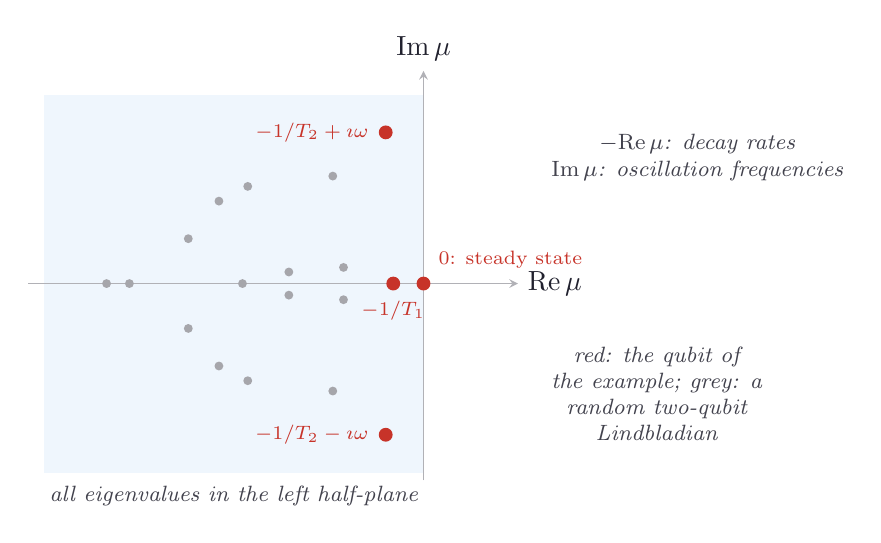
\begin{tikzpicture}[ink/.style={line width=0.9pt, ndInk}, faint/.style={line width=0.4pt, ndInk!35}, dashedink/.style={line width=0.5pt, ndInk!55, dash pattern=on 2.5pt off 2pt}, vec/.style={->, >=stealth, line width=1.2pt}, note/.style={font=\footnotesize\itshape, text=ndInk!85, align=center}, pointer/.style={->, >=stealth, line width=0.4pt, ndInk!60, shorten >=2pt, shorten <=1pt}, dot/.style={circle, fill=ndInk, inner sep=0pt, minimum size=3.4pt}, wash/.style={fill=ndSky, fill opacity=0.55}, every node/.style={text=ndInk}]
\definecolor{ndInk}{rgb}{0.13,0.13,0.18}
\definecolor{ndPaper}{rgb}{0.99,0.96,0.88}
\definecolor{ndSky}{rgb}{0.84,0.91,0.98}
\definecolor{ndRose}{rgb}{0.98,0.86,0.84}
\definecolor{ndBlue}{rgb}{0.13,0.36,0.66}
\definecolor{ndRed}{rgb}{0.78,0.20,0.16}
\definecolor{ndGold}{rgb}{0.88,0.62,0.10}
\definecolor{ndGreen}{rgb}{0.18,0.52,0.30}
\fill[ndSky, fill opacity=0.4] (-4.82,-2.40) rectangle (0,2.40);
\draw[faint, ->, >=stealth] (-5.02,0) -- (1.20,0) node[right, text=ndInk] {$\mathrm{Re}\,\mu$};
\draw[faint, ->, >=stealth] (0,-2.50) -- (0,2.70) node[above, text=ndInk] {$\mathrm{Im}\,\mu$};
\fill[ndInk!40] (0.000,0.000) circle (1.6pt);
\fill[ndInk!40] (-1.152,1.365) circle (1.6pt);
\fill[ndInk!40] (-1.152,-1.365) circle (1.6pt);
\fill[ndInk!40] (-4.025,0.000) circle (1.6pt);
\fill[ndInk!40] (-3.735,-0.000) circle (1.6pt);
\fill[ndInk!40] (-2.232,1.234) circle (1.6pt);
\fill[ndInk!40] (-2.598,1.047) circle (1.6pt);
\fill[ndInk!40] (-2.987,0.570) circle (1.6pt);
\fill[ndInk!40] (-2.232,-1.234) circle (1.6pt);
\fill[ndInk!40] (-2.598,-1.047) circle (1.6pt);
\fill[ndInk!40] (-2.987,-0.570) circle (1.6pt);
\fill[ndInk!40] (-1.016,0.205) circle (1.6pt);
\fill[ndInk!40] (-1.016,-0.205) circle (1.6pt);
\fill[ndInk!40] (-2.299,0.000) circle (1.6pt);
\fill[ndInk!40] (-1.710,0.147) circle (1.6pt);
\fill[ndInk!40] (-1.710,-0.147) circle (1.6pt);
\node[dot, fill=ndRed, minimum size=5pt, label={[font=\scriptsize, text=ndRed]above right:$0$: steady state}] at (0.000,0.000) {};
\node[dot, fill=ndRed, minimum size=5pt, label={[font=\scriptsize, text=ndRed]below:$-1/T_1$}] at (-0.384,0.000) {};
\node[dot, fill=ndRed, minimum size=5pt, label={[font=\scriptsize, text=ndRed]left:$-1/T_2+\imath\omega$}] at (-0.480,1.920) {};
\node[dot, fill=ndRed, minimum size=5pt, label={[font=\scriptsize, text=ndRed]left:$-1/T_2-\imath\omega$}] at (-0.480,-1.920) {};
\node[note, anchor=west] at (1.50,1.60) {$-\mathrm{Re}\,\mu$: decay rates\\ $\mathrm{Im}\,\mu$: oscillation frequencies};
\node[note, anchor=west] at (1.50,-1.40) {red: the qubit of\\ the example; grey: a\\ random two-qubit\\ Lindbladian};
\node[note, anchor=north] at (-2.41,-2.45) {all eigenvalues in the left half-plane};
\end{tikzpicture}
}
\caption{The eigenvalues of the vectorised Lindbladian $\hat\Lind$: the qubit of the example (red) and a random two-qubit Lindbladian (grey). All lie in the closed left half-plane, in conjugate pairs. Generated by \texttt{code/ch03\_spectrum.py}.}\label{fig:ch03:spectrum}
\end{figure}}
\ona{\endgraf\medskip\noindent\textit{Reading the figure.} Each dot is an eigenvalue of the matrix $\hat\Lind$ that generates the evolution. Its horizontal position says how fast a pattern in the state decays (further left means faster), and its vertical position how fast it oscillates. The dot at $0$ belongs to the state that does not change at all, the steady state.\endgraf\smallskip\noindent\textit{Why it matters.} These eigenvalues play the same role as the poles of a linear system in control engineering, or as the eigenvalues of the rate matrix of a continuous-time Markov chain in computer science and probability. The distance between the axis and the nearest non-zero eigenvalue, the \emph{spectral gap}, here $\min(1/T_1,1/T_2)=0.4$, sets how fast the system forgets its initial state, just as the spectral gap of a Markov chain sets its mixing time. Estimating these numbers from measured data is a large part of identification, especially in the frequency domain (\Chap~\ref{C.Frequency}).}
\onp{\begin{center}\resizebox{!}{0.68\textheight}{% Generated by code/needham.py -- do not edit by hand.
\definecolor{qocA}{rgb}{0.00,0.45,0.70}
\definecolor{qocB}{rgb}{0.90,0.60,0.00}
\definecolor{qocC}{rgb}{0.00,0.62,0.45}
\definecolor{qocD}{rgb}{0.80,0.40,0.00}
\definecolor{qocE}{rgb}{0.80,0.60,0.70}
\definecolor{qocF}{rgb}{0.35,0.70,0.90}
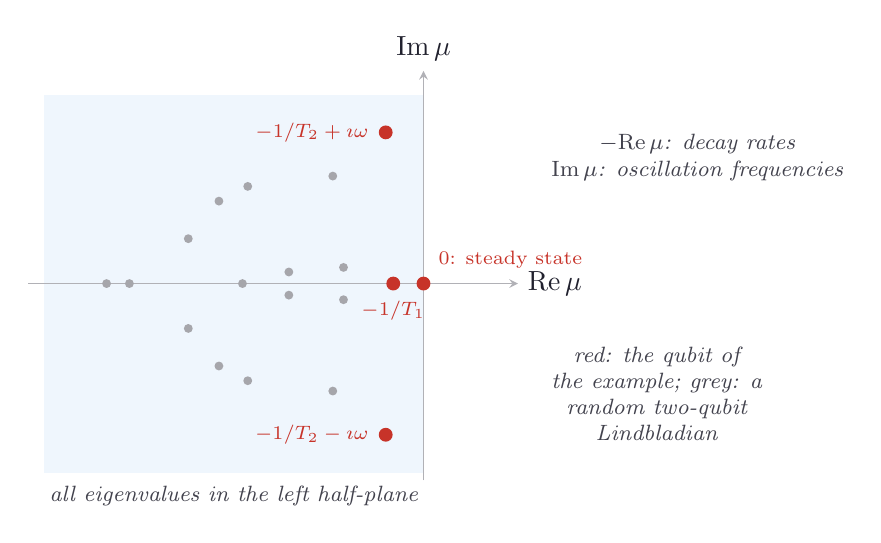
\begin{tikzpicture}[ink/.style={line width=0.9pt, ndInk}, faint/.style={line width=0.4pt, ndInk!35}, dashedink/.style={line width=0.5pt, ndInk!55, dash pattern=on 2.5pt off 2pt}, vec/.style={->, >=stealth, line width=1.2pt}, note/.style={font=\footnotesize\itshape, text=ndInk!85, align=center}, pointer/.style={->, >=stealth, line width=0.4pt, ndInk!60, shorten >=2pt, shorten <=1pt}, dot/.style={circle, fill=ndInk, inner sep=0pt, minimum size=3.4pt}, wash/.style={fill=ndSky, fill opacity=0.55}, every node/.style={text=ndInk}]
\definecolor{ndInk}{rgb}{0.13,0.13,0.18}
\definecolor{ndPaper}{rgb}{0.99,0.96,0.88}
\definecolor{ndSky}{rgb}{0.84,0.91,0.98}
\definecolor{ndRose}{rgb}{0.98,0.86,0.84}
\definecolor{ndBlue}{rgb}{0.13,0.36,0.66}
\definecolor{ndRed}{rgb}{0.78,0.20,0.16}
\definecolor{ndGold}{rgb}{0.88,0.62,0.10}
\definecolor{ndGreen}{rgb}{0.18,0.52,0.30}
\fill[ndSky, fill opacity=0.4] (-4.82,-2.40) rectangle (0,2.40);
\draw[faint, ->, >=stealth] (-5.02,0) -- (1.20,0) node[right, text=ndInk] {$\mathrm{Re}\,\mu$};
\draw[faint, ->, >=stealth] (0,-2.50) -- (0,2.70) node[above, text=ndInk] {$\mathrm{Im}\,\mu$};
\fill[ndInk!40] (0.000,0.000) circle (1.6pt);
\fill[ndInk!40] (-1.152,1.365) circle (1.6pt);
\fill[ndInk!40] (-1.152,-1.365) circle (1.6pt);
\fill[ndInk!40] (-4.025,0.000) circle (1.6pt);
\fill[ndInk!40] (-3.735,-0.000) circle (1.6pt);
\fill[ndInk!40] (-2.232,1.234) circle (1.6pt);
\fill[ndInk!40] (-2.598,1.047) circle (1.6pt);
\fill[ndInk!40] (-2.987,0.570) circle (1.6pt);
\fill[ndInk!40] (-2.232,-1.234) circle (1.6pt);
\fill[ndInk!40] (-2.598,-1.047) circle (1.6pt);
\fill[ndInk!40] (-2.987,-0.570) circle (1.6pt);
\fill[ndInk!40] (-1.016,0.205) circle (1.6pt);
\fill[ndInk!40] (-1.016,-0.205) circle (1.6pt);
\fill[ndInk!40] (-2.299,0.000) circle (1.6pt);
\fill[ndInk!40] (-1.710,0.147) circle (1.6pt);
\fill[ndInk!40] (-1.710,-0.147) circle (1.6pt);
\node[dot, fill=ndRed, minimum size=5pt, label={[font=\scriptsize, text=ndRed]above right:$0$: steady state}] at (0.000,0.000) {};
\node[dot, fill=ndRed, minimum size=5pt, label={[font=\scriptsize, text=ndRed]below:$-1/T_1$}] at (-0.384,0.000) {};
\node[dot, fill=ndRed, minimum size=5pt, label={[font=\scriptsize, text=ndRed]left:$-1/T_2+\imath\omega$}] at (-0.480,1.920) {};
\node[dot, fill=ndRed, minimum size=5pt, label={[font=\scriptsize, text=ndRed]left:$-1/T_2-\imath\omega$}] at (-0.480,-1.920) {};
\node[note, anchor=west] at (1.50,1.60) {$-\mathrm{Re}\,\mu$: decay rates\\ $\mathrm{Im}\,\mu$: oscillation frequencies};
\node[note, anchor=west] at (1.50,-1.40) {red: the qubit of\\ the example; grey: a\\ random two-qubit\\ Lindbladian};
\node[note, anchor=north] at (-2.41,-2.45) {all eigenvalues in the left half-plane};
\end{tikzpicture}
}\end{center}}
\end{frame}

\section{Perturbative master equations}

\begin{frame}\ft{Nakajima--Zwanzig}
\ona{Let us now discuss the second category of master equations, namely the perturbative ones. Famous examples include the Nakajima--Zwanzig \cite{Nakajima1958,Zwanzig1960} and the Schoeller--Sch\"on equations; typically these reduce to the Bloch--Redfield equation, which we derive following \cite{de2017dynamics,Breuer_Petruccione_2010a,Lindar2020lecture}. The usual starting point is the Liouville--von Neumann equation for the complete system in the interaction picture, $\dot \rhofull(t) = -\imath \comm{V_{t}H_{I}}{\rhofull(t)}\eqqcolon g\Lind(t)[\rhofull]$, where $V_{t}X = \ee^{\imath H_{0}t}X\ee^{-\imath H_{0}t}$. One introduces a pair of projection superoperators, $\Pproj\rhofull = \TrB[\rhofull] \otimes \rhoB = \rhoS \otimes \rhoB$ and $\Qproj=\Id-\Pproj$, for some fixed environment state $\rhoB$, splits the equation into its $\Pproj$ and $\Qproj$ parts, formally solves the $\Qproj$ part with a propagator $\mathcal G(t,t_0)$ and substitutes back. This gives the integro-differential \emph{Nakajima--Zwanzig master equation}}
\onp{Interaction picture, $\dot\rhofull=g\Lind(t)[\rhofull]$; projectors $\Pproj\rhofull=\rhoS\otimes\rhoB$, $\Qproj=\Id-\Pproj$. Solve the $\Qproj$-part formally and substitute:}
\begin{equation}\label{eq:ch03:nzme}
    \Pproj\dot\rhofull(t) =
    g\Pproj\Lind(t)\Pproj\rhofull(t)+
     g\Pproj\Lind(t)\mathcal{G}(t,t_0)\Qproj\rhofull(t_0)
    +\int^{t}_{t_0}\Kker_{\textrm{NZ}}(t,\tau)\rhofull(\tau)\,\mathrm{d}\tau,
\end{equation}
\ona{with $\mathcal{G}(t,t_{0}) = T_+\exp[g\int^{t}_{t_0} \Qproj\Lind(\tau)\, \mathrm{d}\tau]$ and the \emph{memory kernel} $\Kker_{\textrm{NZ}}(t,\tau) = g^{2}\Pproj\Lind(t)\mathcal{G}(t,\tau)\Qproj\Lind(\tau)\Pproj$. Setting $\Kker_{\textrm{NZ}}(t,\tau) = \Lind\delta(t-\tau)$ is equivalent to the Markovian approximation. In realistic settings the first term can typically be removed, and if initial separability \eqref{eq:ch03:assump_sep} is assumed, the second term vanishes as well; the remaining equation is the \emph{homogeneous} NZME}
\begin{equation}\label{eq:ch03:nzme-hom}
\Pproj\dot\rhofull(t)=\int_{t_0}^t\Kker_{\rm NZ}(t,\tau)\Pproj\rhofull(\tau)\,\mathrm d\tau .
\end{equation}
\ona{Under the given assumptions the NZME is still \emph{exact}.}
\onp{\begin{itemize}\item memory kernel $\Kker_{\rm NZ}$: exact, non-Markovian, hard to compute; \item $\Kker_{\rm NZ}=\Lind\delta(t-\tau)$ is the Markov approximation; separability kills the inhomogeneous term.\end{itemize}}
\end{frame}

\begin{frame}\ft{Time-convolutionless and Redfield equations}
\ona{The memory kernel in the NZME is often too difficult to compute numerically. An alternative is the \emph{time-convolutionless} (TCL) form, in which the convolution is removed entirely and the equation becomes time-local, $\Pproj\dot\rhofull(t) = \Kker_{\textrm{TCL}}(t)\Pproj\rhofull(t)$, with the memory carried by the time dependence of the generator rather than by an integral over the history \cite{Breuer_Petruccione_2010a,Banchi2018}. Both forms describe the same dynamics, although their perturbative expansions agree only order by order in the coupling.}
\ona{More commonly, the Redfield equation is derived directly in the weak-coupling limit. Formally integrating the interaction-picture equation, substituting, and taking the partial trace gives}
\onp{TCL: time-local, $\Pproj\dot\rhofull=\Kker_{\rm TCL}(t)\Pproj\rhofull$. Redfield: integrate once, trace out $B$, assume $\TrB\comm{V_tH_I}{\rhofull(0)}=0$:}
\begin{equation}\label{eq:ch03:born}
    \dot \rhoS(t) = - \int_{0}^{t} \mathrm{d}\tau\, \TrB\big\{\comm{V_{t}H_{I}}{\comm{V_{\tau}H_{I}}{\rhofull(\tau)}}\big\}.
\end{equation}
\ona{Here we assumed $\TrB\comm{V_{t}H_{I}}{\rhofull(0)} = 0$, which is possible by shifting the environmental operators and assuming initial separability. The system dynamics still depends on $\rhofull(t)$; the \emph{Born approximation} replaces $\rhofull(\tau)\to\rhoS(\tau)\otimes\rhoB$, and the \emph{first Markovian approximation} replaces $\rhoS(\tau) \to \rhoS(t)$. These two approximations give the Redfield equation \cite{REDFIELD19651}}
\onp{Born: $\rhofull(\tau)\to\rhoS(\tau)\otimes\rhoB$; first Markov: $\rhoS(\tau)\to\rhoS(t)$. \alert{Redfield equation}}
\begin{equation}\label{eq:ch03:redfield}
    \dot \rhoS(t) = - \int^{t}_{0} \mathrm{d}\tau\, \TrB\big\{\comm{V_{t}H_{I}}{\comm{V_{\tau}H_{I}}{\rhoS(t) \otimes \rhoB}}\big\}.
\end{equation}
\ona{This equation is infamous for not being able to guarantee a completely positive evolution. The \emph{second Markovian approximation}, replacing $\tau \to t - \tau$ and extending the upper limit to $\infty$, makes it Markovian (with an $O(g^{4}\tau_{B})$ error),}
\onp{Second Markov: $\tau\to t-\tau$, upper limit $\to\infty$:}
\begin{equation}\label{eq:ch03:redfield-markov}
    \dot \rhoS(t) = - \int^{\infty}_{0} \mathrm{d}\tau\, \TrB\big\{\comm{V_{t}H_{I}}{\comm{V_{t-\tau}H_{I}}{\rhoS(t) \otimes \rhoB}}\big\},
\end{equation}
\ona{but even then it is not guaranteed to be a generator of a dynamical semigroup, i.e.\ of GKSL form.}
\onp{Still not guaranteed to be of GKSL form, nor completely positive.}
\end{frame}

\begin{frame}\ft{Secular approximation: from Redfield to Lindblad}\mop{\footnotesize}
\ona{One arrives at a Lindbladian form by a further approximation known as the \emph{secular approximation} or rotating-wave approximation. Substituting $H_I=g\sum_\alpha S_\alpha\otimes B_\alpha$ and the spectral decomposition of the system operators in the frequency domain, $S_{\alpha}(t) = \sum_{\omega}S_{\alpha}(\omega)\ee^{-\imath\omega t}$ over the Bohr frequencies $\omega$, the Markovian Redfield equation reads}
\ona{\begin{equation}
    \dot\rhoS(t) = -g^{2}\sum_{\alpha,\beta}\sum_{\omega,\omega'}\Gamma_{\alpha\beta}(\omega)\ee^{\imath(\omega' - \omega)t}\comm{S^{\dagger}_{\alpha}(\omega')}{S_{\beta}(\omega)\rhoS(t)} + \mathrm{h.c.},
\end{equation}}
\ona{where $\Gamma_{\alpha\beta}(\omega) = \int^{\infty}_{0}\mathrm{d}\tau\, \ee^{\imath\omega\tau}\mathcal{B}_{\alpha\beta}(\tau)$ is the one-sided Fourier transform of the environment correlation function $\mathcal{B}_{\alpha\beta}(\tau) = \Tr[\ee^{\imath H_{B}\tau}B_{\alpha}\ee^{-\imath H_{B}\tau}B_{\beta}\rhoB]$. The secular approximation neglects the rapidly oscillating terms $\omega\ne\omega'$, valid when $|\omega-\omega'|^{-1} \ll \tau_{S}$. Moving back to the Schr\"odinger picture one arrives at}
\onp{Bohr-frequency decomposition $S_\alpha(t)=\sum_\omega S_\alpha(\omega)\ee^{-\imath\omega t}$; drop terms oscillating at $\omega\ne\omega'$ (valid if $|\omega-\omega'|^{-1}\ll\tau_S$). Result:}
\begin{equation}\label{eq:ch03:secular}
\begin{split}
\dot\rhoS(t) = -\imath\Big[ &H_{S} + g^{2}\sum_{\omega}\sum_{\alpha,\beta}\Delta_{\alpha\beta}(\omega)S^{\dagger}_{\alpha}(\omega)S_{\beta}(\omega), \rhoS(t)\Big] \\
&+ g^{2}\sum_{\omega}\sum_{\alpha\beta}\gamma_{\alpha\beta}(\omega)\Big(S_{\beta}(\omega)\rhoS(t)S_{\alpha}^{\dagger}(\omega) - \tfrac{1}{2}\acomm{S_{\alpha}^{\dagger}(\omega)S_{\beta}(\omega)}{\rhoS(t)}\Big),
\end{split}
\end{equation}
\ona{where $\Delta(\omega) = \frac{1}{2\imath}[\Gamma(\omega) - \Gamma^{\dagger}(\omega)]$ is the Lamb shift and $\gamma(\omega) = \Gamma(\omega) + \Gamma^{\dagger}(\omega)$ is the decoherence matrix, the full Fourier transform of the environment correlation function and therefore positive semidefinite. This is of the form \eqref{eq:ch03:gksl}. Neglecting the Lamb shift gives the Bloch--Redfield equation with its tensor $R_{abcd}$. The indiscriminate use of the secular approximation is controversial \cite{Jeske_Bloch_redfield_LHC_2015}; \cite{McCauley2020} showed, using system identification techniques, that Bloch--Redfield dynamics can be replaced by an accurate Lindbladian as long as the spectral density varies sufficiently slowly.}
\onp{Lamb shift $\Delta(\omega)$; decoherence matrix $\gamma(\omega)\succeq0$ (a Fourier transform of a correlation function). This \emph{is} the GKSL form \eqref{eq:ch03:gksl}.}
\end{frame}

\begin{frame}\ft{Why the secular approximation works}
\ona{The secular approximation discards the terms of the Markovian Redfield equation that oscillate at $\ee^{\imath(\omega'-\omega)t}$ with $\omega\ne\omega'$. Figure~\ref{fig:ch03:secular}(a) shows why this is reasonable: over the timescale $\tau_S$ on which the system evolves, such a term averages out, and its running average decays like $1/(\abs{\omega-\omega'}t)$. The terms with $\omega=\omega'$ keep their full weight. The approximation therefore depends on the spectrum of Bohr frequencies, the differences $E_j-E_k$ of the system's energies (panel b). It is accurate when the smallest gap between distinct Bohr frequencies is large compared to $1/\tau_S$. It fails for nearly degenerate gaps, which is the caveat on the Lindblad equation noted in the next frame.}
\ona{\begin{figure}[H]\centering
\resizebox{\linewidth}{!}{% Generated by code/needham.py -- do not edit by hand.
\definecolor{qocA}{rgb}{0.00,0.45,0.70}
\definecolor{qocB}{rgb}{0.90,0.60,0.00}
\definecolor{qocC}{rgb}{0.00,0.62,0.45}
\definecolor{qocD}{rgb}{0.80,0.40,0.00}
\definecolor{qocE}{rgb}{0.80,0.60,0.70}
\definecolor{qocF}{rgb}{0.35,0.70,0.90}
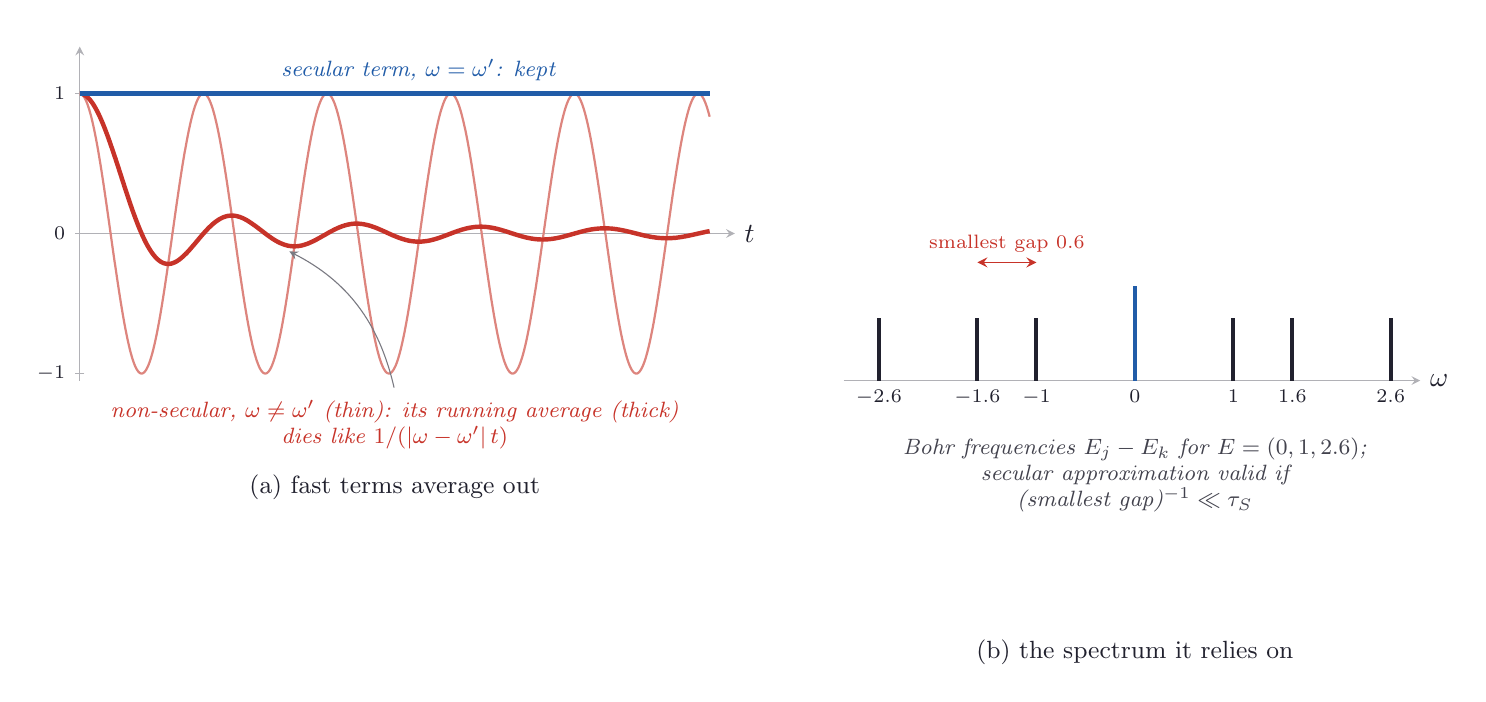
\begin{tikzpicture}[ink/.style={line width=0.9pt, ndInk}, faint/.style={line width=0.4pt, ndInk!35}, dashedink/.style={line width=0.5pt, ndInk!55, dash pattern=on 2.5pt off 2pt}, vec/.style={->, >=stealth, line width=1.2pt}, note/.style={font=\footnotesize\itshape, text=ndInk!85, align=center}, pointer/.style={->, >=stealth, line width=0.4pt, ndInk!60, shorten >=2pt, shorten <=1pt}, dot/.style={circle, fill=ndInk, inner sep=0pt, minimum size=3.4pt}, wash/.style={fill=ndSky, fill opacity=0.55}, every node/.style={text=ndInk}]
\definecolor{ndInk}{rgb}{0.13,0.13,0.18}
\definecolor{ndPaper}{rgb}{0.99,0.96,0.88}
\definecolor{ndSky}{rgb}{0.84,0.91,0.98}
\definecolor{ndRose}{rgb}{0.98,0.86,0.84}
\definecolor{ndBlue}{rgb}{0.13,0.36,0.66}
\definecolor{ndRed}{rgb}{0.78,0.20,0.16}
\definecolor{ndGold}{rgb}{0.88,0.62,0.10}
\definecolor{ndGreen}{rgb}{0.18,0.52,0.30}
\draw[faint, ->, >=stealth] (0.000,1.867) -- (8.320,1.867) node[right, text=ndInk] {$t$};
\draw[faint, ->, >=stealth] (0.000,0.000) -- (0.000,4.240) node[above, text=ndInk] {};
\draw[faint] (0.060,0.089) -- (-0.060,0.089) node[left, font=\scriptsize, text=ndInk] {$-1$};
\draw[faint] (0.060,1.867) -- (-0.060,1.867) node[left, font=\scriptsize, text=ndInk] {$0$};
\draw[faint] (0.060,3.644) -- (-0.060,3.644) node[left, font=\scriptsize, text=ndInk] {$1$};
\draw[line width=0.8pt, ndRed!60] (0.001,3.644) -- (0.011,3.643) -- (0.021,3.638) -- (0.031,3.631) -- (0.041,3.621) -- (0.051,3.607) -- (0.061,3.592) -- (0.071,3.573) -- (0.081,3.552) -- (0.091,3.528) -- (0.101,3.501) -- (0.111,3.472) -- (0.121,3.440) -- (0.131,3.405) -- (0.141,3.369) -- (0.151,3.329) -- (0.161,3.288) -- (0.171,3.244) -- (0.181,3.198) -- (0.191,3.149) -- (0.201,3.099) -- (0.211,3.047) -- (0.221,2.993) -- (0.231,2.937) -- (0.241,2.879) -- (0.251,2.820) -- (0.261,2.759) -- (0.271,2.696) -- (0.281,2.633) -- (0.291,2.568) -- (0.301,2.502) -- (0.311,2.435) -- (0.321,2.367) -- (0.331,2.298) -- (0.341,2.229) -- (0.351,2.159) -- (0.361,2.089) -- (0.371,2.018) -- (0.381,1.947) -- (0.391,1.876) -- (0.401,1.804) -- (0.411,1.733) -- (0.421,1.663) -- (0.431,1.592) -- (0.441,1.522) -- (0.452,1.452) -- (0.462,1.383) -- (0.472,1.315) -- (0.482,1.248) -- (0.492,1.182) -- (0.502,1.117) -- (0.512,1.053) -- (0.522,0.990) -- (0.532,0.929) -- (0.542,0.869) -- (0.552,0.811) -- (0.562,0.755) -- (0.572,0.700) -- (0.582,0.647) -- (0.592,0.597) -- (0.602,0.548) -- (0.612,0.501) -- (0.622,0.457) -- (0.632,0.414) -- (0.642,0.374) -- (0.652,0.337) -- (0.662,0.302) -- (0.672,0.269) -- (0.682,0.239) -- (0.692,0.212) -- (0.702,0.187) -- (0.712,0.165) -- (0.722,0.146) -- (0.732,0.130) -- (0.742,0.116) -- (0.752,0.105) -- (0.762,0.097) -- (0.772,0.091) -- (0.782,0.089) -- (0.792,0.089) -- (0.802,0.093) -- (0.812,0.099) -- (0.822,0.108) -- (0.832,0.120) -- (0.842,0.134) -- (0.852,0.152) -- (0.862,0.172) -- (0.872,0.194) -- (0.882,0.220) -- (0.892,0.248) -- (0.902,0.279) -- (0.912,0.312) -- (0.922,0.348) -- (0.932,0.386) -- (0.942,0.427) -- (0.952,0.470) -- (0.962,0.515) -- (0.972,0.562) -- (0.982,0.611) -- (0.992,0.663) -- (1.002,0.716) -- (1.012,0.771) -- (1.022,0.828) -- (1.032,0.887) -- (1.042,0.947) -- (1.052,1.009) -- (1.062,1.072) -- (1.072,1.136) -- (1.082,1.201) -- (1.092,1.268) -- (1.102,1.335) -- (1.112,1.404) -- (1.122,1.473) -- (1.132,1.543) -- (1.142,1.613) -- (1.152,1.684) -- (1.162,1.754) -- (1.172,1.826) -- (1.182,1.897) -- (1.192,1.968) -- (1.202,2.039) -- (1.212,2.110) -- (1.222,2.180) -- (1.232,2.250) -- (1.242,2.319) -- (1.252,2.387) -- (1.262,2.455) -- (1.272,2.522) -- (1.282,2.587) -- (1.292,2.652) -- (1.302,2.715) -- (1.312,2.777) -- (1.322,2.837) -- (1.332,2.896) -- (1.343,2.953) -- (1.353,3.009) -- (1.363,3.062) -- (1.373,3.114) -- (1.383,3.164) -- (1.393,3.211) -- (1.403,3.257) -- (1.413,3.300) -- (1.423,3.341) -- (1.433,3.380) -- (1.443,3.416) -- (1.453,3.450) -- (1.463,3.481) -- (1.473,3.509) -- (1.483,3.535) -- (1.493,3.558) -- (1.503,3.579) -- (1.513,3.597) -- (1.523,3.612) -- (1.533,3.624) -- (1.543,3.633) -- (1.553,3.640) -- (1.563,3.644) -- (1.573,3.644) -- (1.583,3.642) -- (1.593,3.638) -- (1.603,3.630) -- (1.613,3.619) -- (1.623,3.606) -- (1.633,3.590) -- (1.643,3.571) -- (1.653,3.550) -- (1.663,3.525) -- (1.673,3.498) -- (1.683,3.469) -- (1.693,3.437) -- (1.703,3.402) -- (1.713,3.365) -- (1.723,3.325) -- (1.733,3.283) -- (1.743,3.239) -- (1.753,3.193) -- (1.763,3.145) -- (1.773,3.094) -- (1.783,3.042) -- (1.793,2.987) -- (1.803,2.931) -- (1.813,2.873) -- (1.823,2.814) -- (1.833,2.753) -- (1.843,2.690) -- (1.853,2.627) -- (1.863,2.562) -- (1.873,2.496) -- (1.883,2.428) -- (1.893,2.360) -- (1.903,2.292) -- (1.913,2.222) -- (1.923,2.152) -- (1.933,2.082) -- (1.943,2.011) -- (1.953,1.940) -- (1.963,1.869) -- (1.973,1.798) -- (1.983,1.726) -- (1.993,1.656) -- (2.003,1.585) -- (2.013,1.515) -- (2.023,1.446) -- (2.033,1.377) -- (2.043,1.309) -- (2.053,1.242) -- (2.063,1.176) -- (2.073,1.110) -- (2.083,1.047) -- (2.093,0.984) -- (2.103,0.923) -- (2.113,0.864) -- (2.123,0.806) -- (2.133,0.749) -- (2.143,0.695) -- (2.153,0.642) -- (2.163,0.592) -- (2.173,0.543) -- (2.183,0.497) -- (2.193,0.452) -- (2.203,0.410) -- (2.213,0.371) -- (2.224,0.333) -- (2.234,0.299) -- (2.244,0.266) -- (2.254,0.237) -- (2.264,0.210) -- (2.274,0.185) -- (2.284,0.163) -- (2.294,0.144) -- (2.304,0.128) -- (2.314,0.115) -- (2.324,0.104) -- (2.334,0.096) -- (2.344,0.091) -- (2.354,0.089) -- (2.364,0.090) -- (2.374,0.093) -- (2.384,0.100) -- (2.394,0.109) -- (2.404,0.121) -- (2.414,0.136) -- (2.424,0.153) -- (2.434,0.174) -- (2.444,0.197) -- (2.454,0.223) -- (2.464,0.251) -- (2.474,0.282) -- (2.484,0.315) -- (2.494,0.351) -- (2.504,0.390) -- (2.514,0.431) -- (2.524,0.474) -- (2.534,0.519) -- (2.544,0.567) -- (2.554,0.616) -- (2.564,0.668) -- (2.574,0.721) -- (2.584,0.777) -- (2.594,0.834) -- (2.604,0.893) -- (2.614,0.953) -- (2.624,1.015) -- (2.634,1.078) -- (2.644,1.142) -- (2.654,1.208) -- (2.664,1.274) -- (2.674,1.342) -- (2.684,1.410) -- (2.694,1.480) -- (2.704,1.549) -- (2.714,1.620) -- (2.724,1.690) -- (2.734,1.761) -- (2.744,1.832) -- (2.754,1.904) -- (2.764,1.975) -- (2.774,2.046) -- (2.784,2.116) -- (2.794,2.187) -- (2.804,2.256) -- (2.814,2.326) -- (2.824,2.394) -- (2.834,2.462) -- (2.844,2.528) -- (2.854,2.594) -- (2.864,2.658) -- (2.874,2.721) -- (2.884,2.783) -- (2.894,2.843) -- (2.904,2.902) -- (2.914,2.959) -- (2.924,3.014) -- (2.934,3.068) -- (2.944,3.119) -- (2.954,3.169) -- (2.964,3.216) -- (2.974,3.261) -- (2.984,3.304) -- (2.994,3.345) -- (3.004,3.383) -- (3.014,3.419) -- (3.024,3.453) -- (3.034,3.484) -- (3.044,3.512) -- (3.054,3.537) -- (3.064,3.560) -- (3.074,3.581) -- (3.084,3.598) -- (3.094,3.613) -- (3.104,3.625) -- (3.115,3.634) -- (3.125,3.640) -- (3.135,3.644) -- (3.145,3.644) -- (3.155,3.642) -- (3.165,3.637) -- (3.175,3.629) -- (3.185,3.618) -- (3.195,3.605) -- (3.205,3.588) -- (3.215,3.569) -- (3.225,3.547) -- (3.235,3.523) -- (3.245,3.496) -- (3.255,3.466) -- (3.265,3.433) -- (3.275,3.398) -- (3.285,3.361) -- (3.295,3.321) -- (3.305,3.279) -- (3.315,3.235) -- (3.325,3.188) -- (3.335,3.140) -- (3.345,3.089) -- (3.355,3.036) -- (3.365,2.982) -- (3.375,2.925) -- (3.385,2.867) -- (3.395,2.808) -- (3.405,2.747) -- (3.415,2.684) -- (3.425,2.620) -- (3.435,2.555) -- (3.445,2.489) -- (3.455,2.422) -- (3.465,2.354) -- (3.475,2.285) -- (3.485,2.215) -- (3.495,2.145) -- (3.505,2.075) -- (3.515,2.004) -- (3.525,1.933) -- (3.535,1.862) -- (3.545,1.791) -- (3.555,1.720) -- (3.565,1.649) -- (3.575,1.578) -- (3.585,1.508) -- (3.595,1.439) -- (3.605,1.370) -- (3.615,1.302) -- (3.625,1.235) -- (3.635,1.169) -- (3.645,1.104) -- (3.655,1.041) -- (3.665,0.978) -- (3.675,0.917) -- (3.685,0.858) -- (3.695,0.800) -- (3.705,0.744) -- (3.715,0.690) -- (3.725,0.637) -- (3.735,0.587) -- (3.745,0.538) -- (3.755,0.492) -- (3.765,0.448) -- (3.775,0.406) -- (3.785,0.367) -- (3.795,0.330) -- (3.805,0.295) -- (3.815,0.263) -- (3.825,0.234) -- (3.835,0.207) -- (3.845,0.183) -- (3.855,0.161) -- (3.865,0.143) -- (3.875,0.127) -- (3.885,0.113) -- (3.895,0.103) -- (3.905,0.096) -- (3.915,0.091) -- (3.925,0.089) -- (3.935,0.090) -- (3.945,0.094) -- (3.955,0.100) -- (3.965,0.110) -- (3.975,0.122) -- (3.985,0.137) -- (3.995,0.155) -- (4.006,0.176) -- (4.016,0.199) -- (4.026,0.225) -- (4.036,0.254) -- (4.046,0.285) -- (4.056,0.319) -- (4.066,0.355) -- (4.076,0.394) -- (4.086,0.435) -- (4.096,0.478) -- (4.106,0.524) -- (4.116,0.571) -- (4.126,0.621) -- (4.136,0.673) -- (4.146,0.727) -- (4.156,0.782) -- (4.166,0.839) -- (4.176,0.898) -- (4.186,0.959) -- (4.196,1.021) -- (4.206,1.084) -- (4.216,1.149) -- (4.226,1.214) -- (4.236,1.281) -- (4.246,1.349) -- (4.256,1.417) -- (4.266,1.486) -- (4.276,1.556) -- (4.286,1.627) -- (4.296,1.697) -- (4.306,1.768) -- (4.316,1.839) -- (4.326,1.911) -- (4.336,1.982) -- (4.346,2.053) -- (4.356,2.123) -- (4.366,2.193) -- (4.376,2.263) -- (4.386,2.332) -- (4.396,2.401) -- (4.406,2.468) -- (4.416,2.535) -- (4.426,2.600) -- (4.436,2.664) -- (4.446,2.727) -- (4.456,2.789) -- (4.466,2.849) -- (4.476,2.907) -- (4.486,2.964) -- (4.496,3.019) -- (4.506,3.073) -- (4.516,3.124) -- (4.526,3.173) -- (4.536,3.220) -- (4.546,3.266) -- (4.556,3.308) -- (4.566,3.349) -- (4.576,3.387) -- (4.586,3.423) -- (4.596,3.456) -- (4.606,3.486) -- (4.616,3.514) -- (4.626,3.540) -- (4.636,3.563) -- (4.646,3.583) -- (4.656,3.600) -- (4.666,3.614) -- (4.676,3.626) -- (4.686,3.635) -- (4.696,3.641) -- (4.706,3.644) -- (4.716,3.644) -- (4.726,3.642) -- (4.736,3.636) -- (4.746,3.628) -- (4.756,3.617) -- (4.766,3.603) -- (4.776,3.587) -- (4.786,3.567) -- (4.796,3.545) -- (4.806,3.520) -- (4.816,3.493) -- (4.826,3.463) -- (4.836,3.430) -- (4.846,3.395) -- (4.856,3.357) -- (4.866,3.317) -- (4.876,3.275) -- (4.886,3.230) -- (4.897,3.184) -- (4.907,3.135) -- (4.917,3.084) -- (4.927,3.031) -- (4.937,2.976) -- (4.947,2.920) -- (4.957,2.862) -- (4.967,2.802) -- (4.977,2.741) -- (4.987,2.678) -- (4.997,2.614) -- (5.007,2.549) -- (5.017,2.483) -- (5.027,2.415) -- (5.037,2.347) -- (5.047,2.278) -- (5.057,2.209) -- (5.067,2.139) -- (5.077,2.068) -- (5.087,1.997) -- (5.097,1.926) -- (5.107,1.855) -- (5.117,1.784) -- (5.127,1.713) -- (5.137,1.642) -- (5.147,1.571) -- (5.157,1.502) -- (5.167,1.432) -- (5.177,1.364) -- (5.187,1.296) -- (5.197,1.229) -- (5.207,1.163) -- (5.217,1.098) -- (5.227,1.034) -- (5.237,0.972) -- (5.247,0.911) -- (5.257,0.852) -- (5.267,0.795) -- (5.277,0.739) -- (5.287,0.685) -- (5.297,0.632) -- (5.307,0.582) -- (5.317,0.534) -- (5.327,0.488) -- (5.337,0.444) -- (5.347,0.403) -- (5.357,0.363) -- (5.367,0.327) -- (5.377,0.292) -- (5.387,0.260) -- (5.397,0.231) -- (5.407,0.205) -- (5.417,0.181) -- (5.427,0.159) -- (5.437,0.141) -- (5.447,0.125) -- (5.457,0.112) -- (5.467,0.102) -- (5.477,0.095) -- (5.487,0.090) -- (5.497,0.089) -- (5.507,0.090) -- (5.517,0.094) -- (5.527,0.101) -- (5.537,0.111) -- (5.547,0.124) -- (5.557,0.139) -- (5.567,0.157) -- (5.577,0.178) -- (5.587,0.202) -- (5.597,0.228) -- (5.607,0.257) -- (5.617,0.288) -- (5.627,0.322) -- (5.637,0.359) -- (5.647,0.398) -- (5.657,0.439) -- (5.667,0.482) -- (5.677,0.528) -- (5.687,0.576) -- (5.697,0.626) -- (5.707,0.678) -- (5.717,0.732) -- (5.727,0.788) -- (5.737,0.845) -- (5.747,0.904) -- (5.757,0.965) -- (5.767,1.027) -- (5.777,1.090) -- (5.788,1.155) -- (5.798,1.221) -- (5.808,1.288) -- (5.818,1.355) -- (5.828,1.424) -- (5.838,1.493) -- (5.848,1.563) -- (5.858,1.633) -- (5.868,1.704) -- (5.878,1.775) -- (5.888,1.846) -- (5.898,1.917) -- (5.908,1.989) -- (5.918,2.060) -- (5.928,2.130) -- (5.938,2.200) -- (5.948,2.270) -- (5.958,2.339) -- (5.968,2.407) -- (5.978,2.475) -- (5.988,2.541) -- (5.998,2.606) -- (6.008,2.670) -- (6.018,2.733) -- (6.028,2.795) -- (6.038,2.855) -- (6.048,2.913) -- (6.058,2.970) -- (6.068,3.025) -- (6.078,3.078) -- (6.088,3.129) -- (6.098,3.178) -- (6.108,3.225) -- (6.118,3.270) -- (6.128,3.312) -- (6.138,3.353) -- (6.148,3.390) -- (6.158,3.426) -- (6.168,3.459) -- (6.178,3.489) -- (6.188,3.517) -- (6.198,3.542) -- (6.208,3.565) -- (6.218,3.584) -- (6.228,3.601) -- (6.238,3.616) -- (6.248,3.627) -- (6.258,3.635) -- (6.268,3.641) -- (6.278,3.644) -- (6.288,3.644) -- (6.298,3.641) -- (6.308,3.636) -- (6.318,3.627) -- (6.328,3.616) -- (6.338,3.602) -- (6.348,3.585) -- (6.358,3.565) -- (6.368,3.543) -- (6.378,3.518) -- (6.388,3.490) -- (6.398,3.460) -- (6.408,3.427) -- (6.418,3.391) -- (6.428,3.354) -- (6.438,3.313) -- (6.448,3.271) -- (6.458,3.226) -- (6.468,3.179) -- (6.478,3.130) -- (6.488,3.079) -- (6.498,3.026) -- (6.508,2.971) -- (6.518,2.914) -- (6.528,2.856) -- (6.538,2.796) -- (6.548,2.735) -- (6.558,2.672) -- (6.568,2.608) -- (6.578,2.542) -- (6.588,2.476) -- (6.598,2.409) -- (6.608,2.341) -- (6.618,2.272) -- (6.628,2.202) -- (6.638,2.132) -- (6.648,2.061) -- (6.658,1.990) -- (6.669,1.919) -- (6.679,1.848) -- (6.689,1.777) -- (6.699,1.706) -- (6.709,1.635) -- (6.719,1.565) -- (6.729,1.495) -- (6.739,1.425) -- (6.749,1.357) -- (6.759,1.289) -- (6.769,1.222) -- (6.779,1.156) -- (6.789,1.092) -- (6.799,1.028) -- (6.809,0.966) -- (6.819,0.906) -- (6.829,0.847) -- (6.839,0.789) -- (6.849,0.733) -- (6.859,0.679) -- (6.869,0.627) -- (6.879,0.577) -- (6.889,0.529) -- (6.899,0.484) -- (6.909,0.440) -- (6.919,0.399) -- (6.929,0.360) -- (6.939,0.323) -- (6.949,0.289) -- (6.959,0.257) -- (6.969,0.229) -- (6.979,0.202) -- (6.989,0.179) -- (6.999,0.158) -- (7.009,0.139) -- (7.019,0.124) -- (7.029,0.111) -- (7.039,0.101) -- (7.049,0.094) -- (7.059,0.090) -- (7.069,0.089) -- (7.079,0.090) -- (7.089,0.095) -- (7.099,0.102) -- (7.109,0.112) -- (7.119,0.125) -- (7.129,0.141) -- (7.139,0.159) -- (7.149,0.180) -- (7.159,0.204) -- (7.169,0.231) -- (7.179,0.260) -- (7.189,0.291) -- (7.199,0.326) -- (7.209,0.362) -- (7.219,0.402) -- (7.229,0.443) -- (7.239,0.487) -- (7.249,0.533) -- (7.259,0.581) -- (7.269,0.631) -- (7.279,0.683) -- (7.289,0.737) -- (7.299,0.793) -- (7.309,0.851) -- (7.319,0.910) -- (7.329,0.971) -- (7.339,1.033) -- (7.349,1.097) -- (7.359,1.161) -- (7.369,1.227) -- (7.379,1.294) -- (7.389,1.362) -- (7.399,1.431) -- (7.409,1.500) -- (7.419,1.570) -- (7.429,1.640) -- (7.439,1.711) -- (7.449,1.782) -- (7.459,1.853) -- (7.469,1.924) -- (7.479,1.995) -- (7.489,2.066) -- (7.499,2.137) -- (7.509,2.207) -- (7.519,2.277) -- (7.529,2.346) -- (7.539,2.414) -- (7.549,2.481) -- (7.560,2.547) -- (7.570,2.613) -- (7.580,2.677) -- (7.590,2.739) -- (7.600,2.801) -- (7.610,2.860) -- (7.620,2.919) -- (7.630,2.975) -- (7.640,3.030) -- (7.650,3.083) -- (7.660,3.134) -- (7.670,3.183) -- (7.680,3.229) -- (7.690,3.274) -- (7.700,3.316) -- (7.710,3.356) -- (7.720,3.394) -- (7.730,3.429) -- (7.740,3.462) -- (7.750,3.492) -- (7.760,3.520) -- (7.770,3.544) -- (7.780,3.567) -- (7.790,3.586) -- (7.800,3.603) -- (7.810,3.617) -- (7.820,3.628) -- (7.830,3.636) -- (7.840,3.642) -- (7.850,3.644) -- (7.860,3.644) -- (7.870,3.641) -- (7.880,3.635) -- (7.890,3.626) -- (7.900,3.615) -- (7.910,3.600) -- (7.920,3.583) -- (7.930,3.563) -- (7.940,3.540) -- (7.950,3.515) -- (7.960,3.487) -- (7.970,3.457) -- (7.980,3.423) -- (7.990,3.388) -- (8.000,3.350);
\draw[line width=1.6pt, ndRed] (0.001,3.644) -- (0.011,3.644) -- (0.021,3.642) -- (0.031,3.640) -- (0.041,3.636) -- (0.051,3.632) -- (0.061,3.627) -- (0.071,3.621) -- (0.081,3.613) -- (0.091,3.605) -- (0.101,3.596) -- (0.111,3.586) -- (0.121,3.576) -- (0.131,3.564) -- (0.141,3.551) -- (0.151,3.538) -- (0.161,3.524) -- (0.171,3.509) -- (0.181,3.493) -- (0.191,3.476) -- (0.201,3.459) -- (0.211,3.440) -- (0.221,3.421) -- (0.231,3.402) -- (0.241,3.381) -- (0.251,3.360) -- (0.261,3.338) -- (0.271,3.315) -- (0.281,3.292) -- (0.291,3.269) -- (0.301,3.244) -- (0.311,3.219) -- (0.321,3.194) -- (0.331,3.168) -- (0.341,3.141) -- (0.351,3.114) -- (0.361,3.087) -- (0.371,3.059) -- (0.381,3.031) -- (0.391,3.002) -- (0.401,2.973) -- (0.411,2.944) -- (0.421,2.914) -- (0.431,2.884) -- (0.441,2.854) -- (0.452,2.824) -- (0.462,2.793) -- (0.472,2.763) -- (0.482,2.732) -- (0.492,2.701) -- (0.502,2.670) -- (0.512,2.639) -- (0.522,2.608) -- (0.532,2.577) -- (0.542,2.546) -- (0.552,2.515) -- (0.562,2.484) -- (0.572,2.453) -- (0.582,2.423) -- (0.592,2.392) -- (0.602,2.362) -- (0.612,2.332) -- (0.622,2.302) -- (0.632,2.272) -- (0.642,2.243) -- (0.652,2.214) -- (0.662,2.185) -- (0.672,2.157) -- (0.682,2.129) -- (0.692,2.102) -- (0.702,2.075) -- (0.712,2.048) -- (0.722,2.022) -- (0.732,1.996) -- (0.742,1.971) -- (0.752,1.946) -- (0.762,1.922) -- (0.772,1.898) -- (0.782,1.875) -- (0.792,1.852) -- (0.802,1.830) -- (0.812,1.809) -- (0.822,1.788) -- (0.832,1.768) -- (0.842,1.748) -- (0.852,1.729) -- (0.862,1.711) -- (0.872,1.694) -- (0.882,1.677) -- (0.892,1.661) -- (0.902,1.645) -- (0.912,1.630) -- (0.922,1.616) -- (0.932,1.603) -- (0.942,1.590) -- (0.952,1.578) -- (0.962,1.567) -- (0.972,1.556) -- (0.982,1.546) -- (0.992,1.537) -- (1.002,1.529) -- (1.012,1.521) -- (1.022,1.514) -- (1.032,1.507) -- (1.042,1.502) -- (1.052,1.497) -- (1.062,1.492) -- (1.072,1.489) -- (1.082,1.486) -- (1.092,1.484) -- (1.102,1.482) -- (1.112,1.481) -- (1.122,1.480) -- (1.132,1.481) -- (1.142,1.482) -- (1.152,1.483) -- (1.162,1.485) -- (1.172,1.488) -- (1.182,1.491) -- (1.192,1.495) -- (1.202,1.499) -- (1.212,1.504) -- (1.222,1.509) -- (1.232,1.514) -- (1.242,1.521) -- (1.252,1.527) -- (1.262,1.534) -- (1.272,1.542) -- (1.282,1.550) -- (1.292,1.558) -- (1.302,1.567) -- (1.312,1.576) -- (1.322,1.585) -- (1.332,1.595) -- (1.343,1.605) -- (1.353,1.615) -- (1.363,1.625) -- (1.373,1.636) -- (1.383,1.647) -- (1.393,1.658) -- (1.403,1.669) -- (1.413,1.681) -- (1.423,1.692) -- (1.433,1.704) -- (1.443,1.716) -- (1.453,1.727) -- (1.463,1.739) -- (1.473,1.751) -- (1.483,1.763) -- (1.493,1.775) -- (1.503,1.787) -- (1.513,1.799) -- (1.523,1.811) -- (1.533,1.823) -- (1.543,1.834) -- (1.553,1.846) -- (1.563,1.858) -- (1.573,1.869) -- (1.583,1.880) -- (1.593,1.891) -- (1.603,1.902) -- (1.613,1.913) -- (1.623,1.923) -- (1.633,1.934) -- (1.643,1.944) -- (1.653,1.953) -- (1.663,1.963) -- (1.673,1.972) -- (1.683,1.981) -- (1.693,1.990) -- (1.703,1.998) -- (1.713,2.006) -- (1.723,2.014) -- (1.733,2.022) -- (1.743,2.029) -- (1.753,2.035) -- (1.763,2.042) -- (1.773,2.048) -- (1.783,2.054) -- (1.793,2.059) -- (1.803,2.064) -- (1.813,2.069) -- (1.823,2.073) -- (1.833,2.077) -- (1.843,2.080) -- (1.853,2.083) -- (1.863,2.086) -- (1.873,2.089) -- (1.883,2.091) -- (1.893,2.092) -- (1.903,2.093) -- (1.913,2.094) -- (1.923,2.095) -- (1.933,2.095) -- (1.943,2.095) -- (1.953,2.094) -- (1.963,2.093) -- (1.973,2.092) -- (1.983,2.090) -- (1.993,2.088) -- (2.003,2.086) -- (2.013,2.083) -- (2.023,2.080) -- (2.033,2.077) -- (2.043,2.073) -- (2.053,2.069) -- (2.063,2.065) -- (2.073,2.061) -- (2.083,2.056) -- (2.093,2.051) -- (2.103,2.046) -- (2.113,2.040) -- (2.123,2.035) -- (2.133,2.029) -- (2.143,2.023) -- (2.153,2.016) -- (2.163,2.010) -- (2.173,2.003) -- (2.183,1.996) -- (2.193,1.989) -- (2.203,1.982) -- (2.213,1.975) -- (2.224,1.968) -- (2.234,1.960) -- (2.244,1.953) -- (2.254,1.945) -- (2.264,1.938) -- (2.274,1.930) -- (2.284,1.922) -- (2.294,1.915) -- (2.304,1.907) -- (2.314,1.899) -- (2.324,1.892) -- (2.334,1.884) -- (2.344,1.876) -- (2.354,1.869) -- (2.364,1.861) -- (2.374,1.854) -- (2.384,1.846) -- (2.394,1.839) -- (2.404,1.832) -- (2.414,1.825) -- (2.424,1.818) -- (2.434,1.811) -- (2.444,1.804) -- (2.454,1.798) -- (2.464,1.791) -- (2.474,1.785) -- (2.484,1.779) -- (2.494,1.773) -- (2.504,1.768) -- (2.514,1.762) -- (2.524,1.757) -- (2.534,1.752) -- (2.544,1.747) -- (2.554,1.743) -- (2.564,1.739) -- (2.574,1.735) -- (2.584,1.731) -- (2.594,1.727) -- (2.604,1.724) -- (2.614,1.721) -- (2.624,1.718) -- (2.634,1.715) -- (2.644,1.713) -- (2.654,1.711) -- (2.664,1.709) -- (2.674,1.708) -- (2.684,1.707) -- (2.694,1.706) -- (2.704,1.705) -- (2.714,1.704) -- (2.724,1.704) -- (2.734,1.704) -- (2.744,1.705) -- (2.754,1.705) -- (2.764,1.706) -- (2.774,1.707) -- (2.784,1.709) -- (2.794,1.710) -- (2.804,1.712) -- (2.814,1.714) -- (2.824,1.716) -- (2.834,1.719) -- (2.844,1.722) -- (2.854,1.725) -- (2.864,1.728) -- (2.874,1.731) -- (2.884,1.735) -- (2.894,1.738) -- (2.904,1.742) -- (2.914,1.746) -- (2.924,1.751) -- (2.934,1.755) -- (2.944,1.760) -- (2.954,1.764) -- (2.964,1.769) -- (2.974,1.774) -- (2.984,1.779) -- (2.994,1.784) -- (3.004,1.789) -- (3.014,1.795) -- (3.024,1.800) -- (3.034,1.806) -- (3.044,1.811) -- (3.054,1.817) -- (3.064,1.823) -- (3.074,1.828) -- (3.084,1.834) -- (3.094,1.840) -- (3.104,1.845) -- (3.115,1.851) -- (3.125,1.857) -- (3.135,1.863) -- (3.145,1.868) -- (3.155,1.874) -- (3.165,1.880) -- (3.175,1.885) -- (3.185,1.891) -- (3.195,1.896) -- (3.205,1.901) -- (3.215,1.906) -- (3.225,1.912) -- (3.235,1.917) -- (3.245,1.922) -- (3.255,1.926) -- (3.265,1.931) -- (3.275,1.936) -- (3.285,1.940) -- (3.295,1.944) -- (3.305,1.948) -- (3.315,1.952) -- (3.325,1.956) -- (3.335,1.960) -- (3.345,1.963) -- (3.355,1.966) -- (3.365,1.970) -- (3.375,1.972) -- (3.385,1.975) -- (3.395,1.978) -- (3.405,1.980) -- (3.415,1.982) -- (3.425,1.984) -- (3.435,1.986) -- (3.445,1.988) -- (3.455,1.989) -- (3.465,1.990) -- (3.475,1.991) -- (3.485,1.992) -- (3.495,1.992) -- (3.505,1.993) -- (3.515,1.993) -- (3.525,1.993) -- (3.535,1.992) -- (3.545,1.992) -- (3.555,1.991) -- (3.565,1.990) -- (3.575,1.989) -- (3.585,1.988) -- (3.595,1.987) -- (3.605,1.985) -- (3.615,1.983) -- (3.625,1.981) -- (3.635,1.979) -- (3.645,1.977) -- (3.655,1.974) -- (3.665,1.972) -- (3.675,1.969) -- (3.685,1.966) -- (3.695,1.963) -- (3.705,1.960) -- (3.715,1.956) -- (3.725,1.953) -- (3.735,1.949) -- (3.745,1.946) -- (3.755,1.942) -- (3.765,1.938) -- (3.775,1.934) -- (3.785,1.930) -- (3.795,1.926) -- (3.805,1.921) -- (3.815,1.917) -- (3.825,1.913) -- (3.835,1.908) -- (3.845,1.904) -- (3.855,1.899) -- (3.865,1.895) -- (3.875,1.890) -- (3.885,1.886) -- (3.895,1.881) -- (3.905,1.876) -- (3.915,1.872) -- (3.925,1.867) -- (3.935,1.863) -- (3.945,1.858) -- (3.955,1.854) -- (3.965,1.849) -- (3.975,1.845) -- (3.985,1.841) -- (3.995,1.837) -- (4.006,1.832) -- (4.016,1.828) -- (4.026,1.824) -- (4.036,1.820) -- (4.046,1.816) -- (4.056,1.813) -- (4.066,1.809) -- (4.076,1.806) -- (4.086,1.802) -- (4.096,1.799) -- (4.106,1.796) -- (4.116,1.793) -- (4.126,1.790) -- (4.136,1.787) -- (4.146,1.784) -- (4.156,1.782) -- (4.166,1.780) -- (4.176,1.777) -- (4.186,1.775) -- (4.196,1.773) -- (4.206,1.772) -- (4.216,1.770) -- (4.226,1.769) -- (4.236,1.768) -- (4.246,1.767) -- (4.256,1.766) -- (4.266,1.765) -- (4.276,1.764) -- (4.286,1.764) -- (4.296,1.764) -- (4.306,1.764) -- (4.316,1.764) -- (4.326,1.764) -- (4.336,1.764) -- (4.346,1.765) -- (4.356,1.766) -- (4.366,1.767) -- (4.376,1.768) -- (4.386,1.769) -- (4.396,1.770) -- (4.406,1.772) -- (4.416,1.773) -- (4.426,1.775) -- (4.436,1.777) -- (4.446,1.779) -- (4.456,1.781) -- (4.466,1.784) -- (4.476,1.786) -- (4.486,1.789) -- (4.496,1.791) -- (4.506,1.794) -- (4.516,1.797) -- (4.526,1.800) -- (4.536,1.803) -- (4.546,1.806) -- (4.556,1.810) -- (4.566,1.813) -- (4.576,1.816) -- (4.586,1.820) -- (4.596,1.823) -- (4.606,1.827) -- (4.616,1.831) -- (4.626,1.834) -- (4.636,1.838) -- (4.646,1.842) -- (4.656,1.845) -- (4.666,1.849) -- (4.676,1.853) -- (4.686,1.857) -- (4.696,1.861) -- (4.706,1.864) -- (4.716,1.868) -- (4.726,1.872) -- (4.736,1.876) -- (4.746,1.879) -- (4.756,1.883) -- (4.766,1.887) -- (4.776,1.890) -- (4.786,1.894) -- (4.796,1.897) -- (4.806,1.901) -- (4.816,1.904) -- (4.826,1.907) -- (4.836,1.910) -- (4.846,1.914) -- (4.856,1.917) -- (4.866,1.919) -- (4.876,1.922) -- (4.886,1.925) -- (4.897,1.928) -- (4.907,1.930) -- (4.917,1.933) -- (4.927,1.935) -- (4.937,1.937) -- (4.947,1.939) -- (4.957,1.941) -- (4.967,1.943) -- (4.977,1.944) -- (4.987,1.946) -- (4.997,1.947) -- (5.007,1.949) -- (5.017,1.950) -- (5.027,1.951) -- (5.037,1.952) -- (5.047,1.952) -- (5.057,1.953) -- (5.067,1.953) -- (5.077,1.954) -- (5.087,1.954) -- (5.097,1.954) -- (5.107,1.954) -- (5.117,1.953) -- (5.127,1.953) -- (5.137,1.952) -- (5.147,1.952) -- (5.157,1.951) -- (5.167,1.950) -- (5.177,1.949) -- (5.187,1.948) -- (5.197,1.946) -- (5.207,1.945) -- (5.217,1.943) -- (5.227,1.942) -- (5.237,1.940) -- (5.247,1.938) -- (5.257,1.936) -- (5.267,1.934) -- (5.277,1.932) -- (5.287,1.929) -- (5.297,1.927) -- (5.307,1.925) -- (5.317,1.922) -- (5.327,1.919) -- (5.337,1.917) -- (5.347,1.914) -- (5.357,1.911) -- (5.367,1.908) -- (5.377,1.905) -- (5.387,1.902) -- (5.397,1.899) -- (5.407,1.896) -- (5.417,1.893) -- (5.427,1.890) -- (5.437,1.886) -- (5.447,1.883) -- (5.457,1.880) -- (5.467,1.877) -- (5.477,1.873) -- (5.487,1.870) -- (5.497,1.867) -- (5.507,1.864) -- (5.517,1.860) -- (5.527,1.857) -- (5.537,1.854) -- (5.547,1.851) -- (5.557,1.848) -- (5.567,1.845) -- (5.577,1.842) -- (5.587,1.839) -- (5.597,1.836) -- (5.607,1.833) -- (5.617,1.830) -- (5.627,1.828) -- (5.637,1.825) -- (5.647,1.822) -- (5.657,1.820) -- (5.667,1.817) -- (5.677,1.815) -- (5.687,1.813) -- (5.697,1.811) -- (5.707,1.809) -- (5.717,1.807) -- (5.727,1.805) -- (5.737,1.803) -- (5.747,1.802) -- (5.757,1.800) -- (5.767,1.799) -- (5.777,1.797) -- (5.788,1.796) -- (5.798,1.795) -- (5.808,1.794) -- (5.818,1.793) -- (5.828,1.793) -- (5.838,1.792) -- (5.848,1.792) -- (5.858,1.791) -- (5.868,1.791) -- (5.878,1.791) -- (5.888,1.791) -- (5.898,1.791) -- (5.908,1.792) -- (5.918,1.792) -- (5.928,1.793) -- (5.938,1.793) -- (5.948,1.794) -- (5.958,1.795) -- (5.968,1.796) -- (5.978,1.797) -- (5.988,1.798) -- (5.998,1.799) -- (6.008,1.801) -- (6.018,1.802) -- (6.028,1.804) -- (6.038,1.805) -- (6.048,1.807) -- (6.058,1.809) -- (6.068,1.811) -- (6.078,1.813) -- (6.088,1.815) -- (6.098,1.817) -- (6.108,1.820) -- (6.118,1.822) -- (6.128,1.824) -- (6.138,1.827) -- (6.148,1.829) -- (6.158,1.832) -- (6.168,1.835) -- (6.178,1.837) -- (6.188,1.840) -- (6.198,1.843) -- (6.208,1.845) -- (6.218,1.848) -- (6.228,1.851) -- (6.238,1.854) -- (6.248,1.857) -- (6.258,1.860) -- (6.268,1.862) -- (6.278,1.865) -- (6.288,1.868) -- (6.298,1.871) -- (6.308,1.874) -- (6.318,1.876) -- (6.328,1.879) -- (6.338,1.882) -- (6.348,1.885) -- (6.358,1.887) -- (6.368,1.890) -- (6.378,1.893) -- (6.388,1.895) -- (6.398,1.898) -- (6.408,1.900) -- (6.418,1.902) -- (6.428,1.905) -- (6.438,1.907) -- (6.448,1.909) -- (6.458,1.911) -- (6.468,1.913) -- (6.478,1.915) -- (6.488,1.917) -- (6.498,1.919) -- (6.508,1.920) -- (6.518,1.922) -- (6.528,1.923) -- (6.538,1.925) -- (6.548,1.926) -- (6.558,1.927) -- (6.568,1.928) -- (6.578,1.929) -- (6.588,1.930) -- (6.598,1.931) -- (6.608,1.931) -- (6.618,1.932) -- (6.628,1.933) -- (6.638,1.933) -- (6.648,1.933) -- (6.658,1.933) -- (6.669,1.933) -- (6.679,1.933) -- (6.689,1.933) -- (6.699,1.933) -- (6.709,1.932) -- (6.719,1.932) -- (6.729,1.931) -- (6.739,1.931) -- (6.749,1.930) -- (6.759,1.929) -- (6.769,1.928) -- (6.779,1.927) -- (6.789,1.926) -- (6.799,1.924) -- (6.809,1.923) -- (6.819,1.922) -- (6.829,1.920) -- (6.839,1.918) -- (6.849,1.917) -- (6.859,1.915) -- (6.869,1.913) -- (6.879,1.911) -- (6.889,1.909) -- (6.899,1.907) -- (6.909,1.905) -- (6.919,1.903) -- (6.929,1.901) -- (6.939,1.898) -- (6.949,1.896) -- (6.959,1.894) -- (6.969,1.891) -- (6.979,1.889) -- (6.989,1.887) -- (6.999,1.884) -- (7.009,1.882) -- (7.019,1.879) -- (7.029,1.877) -- (7.039,1.874) -- (7.049,1.872) -- (7.059,1.869) -- (7.069,1.867) -- (7.079,1.864) -- (7.089,1.862) -- (7.099,1.859) -- (7.109,1.857) -- (7.119,1.854) -- (7.129,1.852) -- (7.139,1.849) -- (7.149,1.847) -- (7.159,1.845) -- (7.169,1.842) -- (7.179,1.840) -- (7.189,1.838) -- (7.199,1.836) -- (7.209,1.834) -- (7.219,1.832) -- (7.229,1.830) -- (7.239,1.828) -- (7.249,1.826) -- (7.259,1.824) -- (7.269,1.823) -- (7.279,1.821) -- (7.289,1.820) -- (7.299,1.818) -- (7.309,1.817) -- (7.319,1.815) -- (7.329,1.814) -- (7.339,1.813) -- (7.349,1.812) -- (7.359,1.811) -- (7.369,1.810) -- (7.379,1.810) -- (7.389,1.809) -- (7.399,1.808) -- (7.409,1.808) -- (7.419,1.808) -- (7.429,1.807) -- (7.439,1.807) -- (7.449,1.807) -- (7.459,1.807) -- (7.469,1.807) -- (7.479,1.807) -- (7.489,1.808) -- (7.499,1.808) -- (7.509,1.809) -- (7.519,1.809) -- (7.529,1.810) -- (7.539,1.811) -- (7.549,1.811) -- (7.560,1.812) -- (7.570,1.813) -- (7.580,1.814) -- (7.590,1.816) -- (7.600,1.817) -- (7.610,1.818) -- (7.620,1.820) -- (7.630,1.821) -- (7.640,1.823) -- (7.650,1.824) -- (7.660,1.826) -- (7.670,1.828) -- (7.680,1.830) -- (7.690,1.831) -- (7.700,1.833) -- (7.710,1.835) -- (7.720,1.837) -- (7.730,1.839) -- (7.740,1.841) -- (7.750,1.843) -- (7.760,1.846) -- (7.770,1.848) -- (7.780,1.850) -- (7.790,1.852) -- (7.800,1.854) -- (7.810,1.857) -- (7.820,1.859) -- (7.830,1.861) -- (7.840,1.863) -- (7.850,1.866) -- (7.860,1.868) -- (7.870,1.870) -- (7.880,1.872) -- (7.890,1.875) -- (7.900,1.877) -- (7.910,1.879) -- (7.920,1.881) -- (7.930,1.883) -- (7.940,1.886) -- (7.950,1.888) -- (7.960,1.890) -- (7.970,1.892) -- (7.980,1.894) -- (7.990,1.895) -- (8.000,1.897);
\draw[line width=1.6pt, ndBlue] (0.000,3.644) -- (8.000,3.644);
\node[note, anchor=south, text=ndBlue] at (4.300,3.680) {secular term, $\omega=\omega'$: kept};
\node[note, anchor=north, text=ndRed] (n) at (4.000,-0.124) {non-secular, $\omega\ne\omega'$ (thin): its running average (thick)\\ dies like $1/(|\omega-\omega'|\,t)$};
\draw[pointer] (n.north) to[bend right=25] (2.600,1.671);
\node[font=\small] at (4.000,-1.350) {(a) fast terms average out};
\draw[faint, ->, >=stealth] (9.700,0.000) -- (17.025,0.000) node[right, text=ndInk] {$\omega$};
\draw[line width=1.4pt, ndInk] (10.150,0.000) -- (10.150,0.800);
\node[font=\scriptsize, below] at (10.150,0.000) {$-2.6$};
\draw[line width=1.4pt, ndInk] (11.400,0.000) -- (11.400,0.800);
\node[font=\scriptsize, below] at (11.400,0.000) {$-1.6$};
\draw[line width=1.4pt, ndInk] (12.150,0.000) -- (12.150,0.800);
\node[font=\scriptsize, below] at (12.150,0.000) {$-1$};
\draw[line width=1.4pt, ndBlue] (13.400,0.000) -- (13.400,1.200);
\node[font=\scriptsize, below] at (13.400,0.000) {$0$};
\draw[line width=1.4pt, ndInk] (14.650,0.000) -- (14.650,0.800);
\node[font=\scriptsize, below] at (14.650,0.000) {$1$};
\draw[line width=1.4pt, ndInk] (15.400,0.000) -- (15.400,0.800);
\node[font=\scriptsize, below] at (15.400,0.000) {$1.6$};
\draw[line width=1.4pt, ndInk] (16.650,0.000) -- (16.650,0.800);
\node[font=\scriptsize, below] at (16.650,0.000) {$2.6$};
\draw[<->, >=stealth, line width=0.6pt, ndRed] (11.400,1.500) -- (12.150,1.500) node[midway, above, font=\scriptsize, text=ndRed] {smallest gap $0.6$};
\node[note, anchor=north] at (13.400,-0.600) {Bohr frequencies $E_j-E_k$ for $E=(0,1,2.6)$;\\ secular approximation valid if\\ (smallest gap)$^{-1}\ll\tau_S$};
\node[font=\small] at (13.400,-3.450) {(b) the spectrum it relies on};
\end{tikzpicture}
}
\caption{(a) A non-secular term $\cos((\omega'-\omega)t)$ (thin) and its running average (thick), which vanishes, against a secular term that is kept. (b) The Bohr frequencies of a three-level system with energies $(0,1,2.6)$ and their smallest gap. Generated by \texttt{code/ch03\_secular.py}.}\label{fig:ch03:secular}
\end{figure}}
\ona{\endgraf\medskip\noindent\textit{Reading the figure.} In panel (a), the thin red curve is a term of the Redfield equation that oscillates quickly; the thick red curve is its average from time $0$ up to $t$, which tends to zero; the blue line is a term that does not oscillate and is kept. In panel (b), each stem is one possible energy difference (Bohr frequency) of a three-level system, and the arrow marks the smallest separation between two distinct ones.\endgraf\smallskip\noindent\textit{Why it matters.} The secular approximation is what turns the Redfield equation into a Lindblad equation, and only the latter is guaranteed to produce valid density matrices. Computer scientists may think of it as a low-pass filter that removes high-frequency components. Whether it is justified is a statement about the spectrum in panel (b): it works when distinct frequencies are well separated compared with the decay rates, and fails for nearly degenerate ones. In many-qubit chips, whose qubits are deliberately given similar frequencies, this ``frequency crowding'' is a practical concern.}
\onp{\begin{center}\resizebox{\linewidth}{!}{% Generated by code/needham.py -- do not edit by hand.
\definecolor{qocA}{rgb}{0.00,0.45,0.70}
\definecolor{qocB}{rgb}{0.90,0.60,0.00}
\definecolor{qocC}{rgb}{0.00,0.62,0.45}
\definecolor{qocD}{rgb}{0.80,0.40,0.00}
\definecolor{qocE}{rgb}{0.80,0.60,0.70}
\definecolor{qocF}{rgb}{0.35,0.70,0.90}
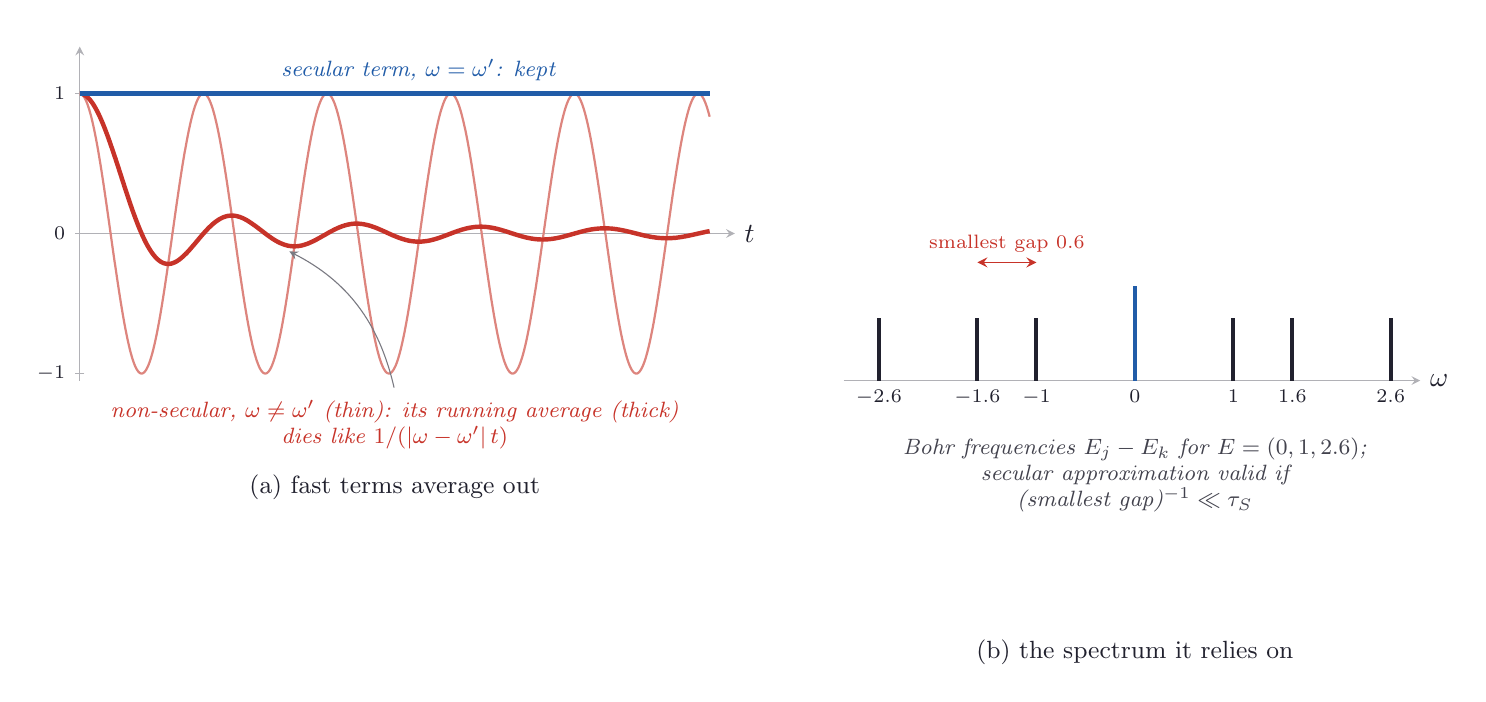
\begin{tikzpicture}[ink/.style={line width=0.9pt, ndInk}, faint/.style={line width=0.4pt, ndInk!35}, dashedink/.style={line width=0.5pt, ndInk!55, dash pattern=on 2.5pt off 2pt}, vec/.style={->, >=stealth, line width=1.2pt}, note/.style={font=\footnotesize\itshape, text=ndInk!85, align=center}, pointer/.style={->, >=stealth, line width=0.4pt, ndInk!60, shorten >=2pt, shorten <=1pt}, dot/.style={circle, fill=ndInk, inner sep=0pt, minimum size=3.4pt}, wash/.style={fill=ndSky, fill opacity=0.55}, every node/.style={text=ndInk}]
\definecolor{ndInk}{rgb}{0.13,0.13,0.18}
\definecolor{ndPaper}{rgb}{0.99,0.96,0.88}
\definecolor{ndSky}{rgb}{0.84,0.91,0.98}
\definecolor{ndRose}{rgb}{0.98,0.86,0.84}
\definecolor{ndBlue}{rgb}{0.13,0.36,0.66}
\definecolor{ndRed}{rgb}{0.78,0.20,0.16}
\definecolor{ndGold}{rgb}{0.88,0.62,0.10}
\definecolor{ndGreen}{rgb}{0.18,0.52,0.30}
\draw[faint, ->, >=stealth] (0.000,1.867) -- (8.320,1.867) node[right, text=ndInk] {$t$};
\draw[faint, ->, >=stealth] (0.000,0.000) -- (0.000,4.240) node[above, text=ndInk] {};
\draw[faint] (0.060,0.089) -- (-0.060,0.089) node[left, font=\scriptsize, text=ndInk] {$-1$};
\draw[faint] (0.060,1.867) -- (-0.060,1.867) node[left, font=\scriptsize, text=ndInk] {$0$};
\draw[faint] (0.060,3.644) -- (-0.060,3.644) node[left, font=\scriptsize, text=ndInk] {$1$};
\draw[line width=0.8pt, ndRed!60] (0.001,3.644) -- (0.011,3.643) -- (0.021,3.638) -- (0.031,3.631) -- (0.041,3.621) -- (0.051,3.607) -- (0.061,3.592) -- (0.071,3.573) -- (0.081,3.552) -- (0.091,3.528) -- (0.101,3.501) -- (0.111,3.472) -- (0.121,3.440) -- (0.131,3.405) -- (0.141,3.369) -- (0.151,3.329) -- (0.161,3.288) -- (0.171,3.244) -- (0.181,3.198) -- (0.191,3.149) -- (0.201,3.099) -- (0.211,3.047) -- (0.221,2.993) -- (0.231,2.937) -- (0.241,2.879) -- (0.251,2.820) -- (0.261,2.759) -- (0.271,2.696) -- (0.281,2.633) -- (0.291,2.568) -- (0.301,2.502) -- (0.311,2.435) -- (0.321,2.367) -- (0.331,2.298) -- (0.341,2.229) -- (0.351,2.159) -- (0.361,2.089) -- (0.371,2.018) -- (0.381,1.947) -- (0.391,1.876) -- (0.401,1.804) -- (0.411,1.733) -- (0.421,1.663) -- (0.431,1.592) -- (0.441,1.522) -- (0.452,1.452) -- (0.462,1.383) -- (0.472,1.315) -- (0.482,1.248) -- (0.492,1.182) -- (0.502,1.117) -- (0.512,1.053) -- (0.522,0.990) -- (0.532,0.929) -- (0.542,0.869) -- (0.552,0.811) -- (0.562,0.755) -- (0.572,0.700) -- (0.582,0.647) -- (0.592,0.597) -- (0.602,0.548) -- (0.612,0.501) -- (0.622,0.457) -- (0.632,0.414) -- (0.642,0.374) -- (0.652,0.337) -- (0.662,0.302) -- (0.672,0.269) -- (0.682,0.239) -- (0.692,0.212) -- (0.702,0.187) -- (0.712,0.165) -- (0.722,0.146) -- (0.732,0.130) -- (0.742,0.116) -- (0.752,0.105) -- (0.762,0.097) -- (0.772,0.091) -- (0.782,0.089) -- (0.792,0.089) -- (0.802,0.093) -- (0.812,0.099) -- (0.822,0.108) -- (0.832,0.120) -- (0.842,0.134) -- (0.852,0.152) -- (0.862,0.172) -- (0.872,0.194) -- (0.882,0.220) -- (0.892,0.248) -- (0.902,0.279) -- (0.912,0.312) -- (0.922,0.348) -- (0.932,0.386) -- (0.942,0.427) -- (0.952,0.470) -- (0.962,0.515) -- (0.972,0.562) -- (0.982,0.611) -- (0.992,0.663) -- (1.002,0.716) -- (1.012,0.771) -- (1.022,0.828) -- (1.032,0.887) -- (1.042,0.947) -- (1.052,1.009) -- (1.062,1.072) -- (1.072,1.136) -- (1.082,1.201) -- (1.092,1.268) -- (1.102,1.335) -- (1.112,1.404) -- (1.122,1.473) -- (1.132,1.543) -- (1.142,1.613) -- (1.152,1.684) -- (1.162,1.754) -- (1.172,1.826) -- (1.182,1.897) -- (1.192,1.968) -- (1.202,2.039) -- (1.212,2.110) -- (1.222,2.180) -- (1.232,2.250) -- (1.242,2.319) -- (1.252,2.387) -- (1.262,2.455) -- (1.272,2.522) -- (1.282,2.587) -- (1.292,2.652) -- (1.302,2.715) -- (1.312,2.777) -- (1.322,2.837) -- (1.332,2.896) -- (1.343,2.953) -- (1.353,3.009) -- (1.363,3.062) -- (1.373,3.114) -- (1.383,3.164) -- (1.393,3.211) -- (1.403,3.257) -- (1.413,3.300) -- (1.423,3.341) -- (1.433,3.380) -- (1.443,3.416) -- (1.453,3.450) -- (1.463,3.481) -- (1.473,3.509) -- (1.483,3.535) -- (1.493,3.558) -- (1.503,3.579) -- (1.513,3.597) -- (1.523,3.612) -- (1.533,3.624) -- (1.543,3.633) -- (1.553,3.640) -- (1.563,3.644) -- (1.573,3.644) -- (1.583,3.642) -- (1.593,3.638) -- (1.603,3.630) -- (1.613,3.619) -- (1.623,3.606) -- (1.633,3.590) -- (1.643,3.571) -- (1.653,3.550) -- (1.663,3.525) -- (1.673,3.498) -- (1.683,3.469) -- (1.693,3.437) -- (1.703,3.402) -- (1.713,3.365) -- (1.723,3.325) -- (1.733,3.283) -- (1.743,3.239) -- (1.753,3.193) -- (1.763,3.145) -- (1.773,3.094) -- (1.783,3.042) -- (1.793,2.987) -- (1.803,2.931) -- (1.813,2.873) -- (1.823,2.814) -- (1.833,2.753) -- (1.843,2.690) -- (1.853,2.627) -- (1.863,2.562) -- (1.873,2.496) -- (1.883,2.428) -- (1.893,2.360) -- (1.903,2.292) -- (1.913,2.222) -- (1.923,2.152) -- (1.933,2.082) -- (1.943,2.011) -- (1.953,1.940) -- (1.963,1.869) -- (1.973,1.798) -- (1.983,1.726) -- (1.993,1.656) -- (2.003,1.585) -- (2.013,1.515) -- (2.023,1.446) -- (2.033,1.377) -- (2.043,1.309) -- (2.053,1.242) -- (2.063,1.176) -- (2.073,1.110) -- (2.083,1.047) -- (2.093,0.984) -- (2.103,0.923) -- (2.113,0.864) -- (2.123,0.806) -- (2.133,0.749) -- (2.143,0.695) -- (2.153,0.642) -- (2.163,0.592) -- (2.173,0.543) -- (2.183,0.497) -- (2.193,0.452) -- (2.203,0.410) -- (2.213,0.371) -- (2.224,0.333) -- (2.234,0.299) -- (2.244,0.266) -- (2.254,0.237) -- (2.264,0.210) -- (2.274,0.185) -- (2.284,0.163) -- (2.294,0.144) -- (2.304,0.128) -- (2.314,0.115) -- (2.324,0.104) -- (2.334,0.096) -- (2.344,0.091) -- (2.354,0.089) -- (2.364,0.090) -- (2.374,0.093) -- (2.384,0.100) -- (2.394,0.109) -- (2.404,0.121) -- (2.414,0.136) -- (2.424,0.153) -- (2.434,0.174) -- (2.444,0.197) -- (2.454,0.223) -- (2.464,0.251) -- (2.474,0.282) -- (2.484,0.315) -- (2.494,0.351) -- (2.504,0.390) -- (2.514,0.431) -- (2.524,0.474) -- (2.534,0.519) -- (2.544,0.567) -- (2.554,0.616) -- (2.564,0.668) -- (2.574,0.721) -- (2.584,0.777) -- (2.594,0.834) -- (2.604,0.893) -- (2.614,0.953) -- (2.624,1.015) -- (2.634,1.078) -- (2.644,1.142) -- (2.654,1.208) -- (2.664,1.274) -- (2.674,1.342) -- (2.684,1.410) -- (2.694,1.480) -- (2.704,1.549) -- (2.714,1.620) -- (2.724,1.690) -- (2.734,1.761) -- (2.744,1.832) -- (2.754,1.904) -- (2.764,1.975) -- (2.774,2.046) -- (2.784,2.116) -- (2.794,2.187) -- (2.804,2.256) -- (2.814,2.326) -- (2.824,2.394) -- (2.834,2.462) -- (2.844,2.528) -- (2.854,2.594) -- (2.864,2.658) -- (2.874,2.721) -- (2.884,2.783) -- (2.894,2.843) -- (2.904,2.902) -- (2.914,2.959) -- (2.924,3.014) -- (2.934,3.068) -- (2.944,3.119) -- (2.954,3.169) -- (2.964,3.216) -- (2.974,3.261) -- (2.984,3.304) -- (2.994,3.345) -- (3.004,3.383) -- (3.014,3.419) -- (3.024,3.453) -- (3.034,3.484) -- (3.044,3.512) -- (3.054,3.537) -- (3.064,3.560) -- (3.074,3.581) -- (3.084,3.598) -- (3.094,3.613) -- (3.104,3.625) -- (3.115,3.634) -- (3.125,3.640) -- (3.135,3.644) -- (3.145,3.644) -- (3.155,3.642) -- (3.165,3.637) -- (3.175,3.629) -- (3.185,3.618) -- (3.195,3.605) -- (3.205,3.588) -- (3.215,3.569) -- (3.225,3.547) -- (3.235,3.523) -- (3.245,3.496) -- (3.255,3.466) -- (3.265,3.433) -- (3.275,3.398) -- (3.285,3.361) -- (3.295,3.321) -- (3.305,3.279) -- (3.315,3.235) -- (3.325,3.188) -- (3.335,3.140) -- (3.345,3.089) -- (3.355,3.036) -- (3.365,2.982) -- (3.375,2.925) -- (3.385,2.867) -- (3.395,2.808) -- (3.405,2.747) -- (3.415,2.684) -- (3.425,2.620) -- (3.435,2.555) -- (3.445,2.489) -- (3.455,2.422) -- (3.465,2.354) -- (3.475,2.285) -- (3.485,2.215) -- (3.495,2.145) -- (3.505,2.075) -- (3.515,2.004) -- (3.525,1.933) -- (3.535,1.862) -- (3.545,1.791) -- (3.555,1.720) -- (3.565,1.649) -- (3.575,1.578) -- (3.585,1.508) -- (3.595,1.439) -- (3.605,1.370) -- (3.615,1.302) -- (3.625,1.235) -- (3.635,1.169) -- (3.645,1.104) -- (3.655,1.041) -- (3.665,0.978) -- (3.675,0.917) -- (3.685,0.858) -- (3.695,0.800) -- (3.705,0.744) -- (3.715,0.690) -- (3.725,0.637) -- (3.735,0.587) -- (3.745,0.538) -- (3.755,0.492) -- (3.765,0.448) -- (3.775,0.406) -- (3.785,0.367) -- (3.795,0.330) -- (3.805,0.295) -- (3.815,0.263) -- (3.825,0.234) -- (3.835,0.207) -- (3.845,0.183) -- (3.855,0.161) -- (3.865,0.143) -- (3.875,0.127) -- (3.885,0.113) -- (3.895,0.103) -- (3.905,0.096) -- (3.915,0.091) -- (3.925,0.089) -- (3.935,0.090) -- (3.945,0.094) -- (3.955,0.100) -- (3.965,0.110) -- (3.975,0.122) -- (3.985,0.137) -- (3.995,0.155) -- (4.006,0.176) -- (4.016,0.199) -- (4.026,0.225) -- (4.036,0.254) -- (4.046,0.285) -- (4.056,0.319) -- (4.066,0.355) -- (4.076,0.394) -- (4.086,0.435) -- (4.096,0.478) -- (4.106,0.524) -- (4.116,0.571) -- (4.126,0.621) -- (4.136,0.673) -- (4.146,0.727) -- (4.156,0.782) -- (4.166,0.839) -- (4.176,0.898) -- (4.186,0.959) -- (4.196,1.021) -- (4.206,1.084) -- (4.216,1.149) -- (4.226,1.214) -- (4.236,1.281) -- (4.246,1.349) -- (4.256,1.417) -- (4.266,1.486) -- (4.276,1.556) -- (4.286,1.627) -- (4.296,1.697) -- (4.306,1.768) -- (4.316,1.839) -- (4.326,1.911) -- (4.336,1.982) -- (4.346,2.053) -- (4.356,2.123) -- (4.366,2.193) -- (4.376,2.263) -- (4.386,2.332) -- (4.396,2.401) -- (4.406,2.468) -- (4.416,2.535) -- (4.426,2.600) -- (4.436,2.664) -- (4.446,2.727) -- (4.456,2.789) -- (4.466,2.849) -- (4.476,2.907) -- (4.486,2.964) -- (4.496,3.019) -- (4.506,3.073) -- (4.516,3.124) -- (4.526,3.173) -- (4.536,3.220) -- (4.546,3.266) -- (4.556,3.308) -- (4.566,3.349) -- (4.576,3.387) -- (4.586,3.423) -- (4.596,3.456) -- (4.606,3.486) -- (4.616,3.514) -- (4.626,3.540) -- (4.636,3.563) -- (4.646,3.583) -- (4.656,3.600) -- (4.666,3.614) -- (4.676,3.626) -- (4.686,3.635) -- (4.696,3.641) -- (4.706,3.644) -- (4.716,3.644) -- (4.726,3.642) -- (4.736,3.636) -- (4.746,3.628) -- (4.756,3.617) -- (4.766,3.603) -- (4.776,3.587) -- (4.786,3.567) -- (4.796,3.545) -- (4.806,3.520) -- (4.816,3.493) -- (4.826,3.463) -- (4.836,3.430) -- (4.846,3.395) -- (4.856,3.357) -- (4.866,3.317) -- (4.876,3.275) -- (4.886,3.230) -- (4.897,3.184) -- (4.907,3.135) -- (4.917,3.084) -- (4.927,3.031) -- (4.937,2.976) -- (4.947,2.920) -- (4.957,2.862) -- (4.967,2.802) -- (4.977,2.741) -- (4.987,2.678) -- (4.997,2.614) -- (5.007,2.549) -- (5.017,2.483) -- (5.027,2.415) -- (5.037,2.347) -- (5.047,2.278) -- (5.057,2.209) -- (5.067,2.139) -- (5.077,2.068) -- (5.087,1.997) -- (5.097,1.926) -- (5.107,1.855) -- (5.117,1.784) -- (5.127,1.713) -- (5.137,1.642) -- (5.147,1.571) -- (5.157,1.502) -- (5.167,1.432) -- (5.177,1.364) -- (5.187,1.296) -- (5.197,1.229) -- (5.207,1.163) -- (5.217,1.098) -- (5.227,1.034) -- (5.237,0.972) -- (5.247,0.911) -- (5.257,0.852) -- (5.267,0.795) -- (5.277,0.739) -- (5.287,0.685) -- (5.297,0.632) -- (5.307,0.582) -- (5.317,0.534) -- (5.327,0.488) -- (5.337,0.444) -- (5.347,0.403) -- (5.357,0.363) -- (5.367,0.327) -- (5.377,0.292) -- (5.387,0.260) -- (5.397,0.231) -- (5.407,0.205) -- (5.417,0.181) -- (5.427,0.159) -- (5.437,0.141) -- (5.447,0.125) -- (5.457,0.112) -- (5.467,0.102) -- (5.477,0.095) -- (5.487,0.090) -- (5.497,0.089) -- (5.507,0.090) -- (5.517,0.094) -- (5.527,0.101) -- (5.537,0.111) -- (5.547,0.124) -- (5.557,0.139) -- (5.567,0.157) -- (5.577,0.178) -- (5.587,0.202) -- (5.597,0.228) -- (5.607,0.257) -- (5.617,0.288) -- (5.627,0.322) -- (5.637,0.359) -- (5.647,0.398) -- (5.657,0.439) -- (5.667,0.482) -- (5.677,0.528) -- (5.687,0.576) -- (5.697,0.626) -- (5.707,0.678) -- (5.717,0.732) -- (5.727,0.788) -- (5.737,0.845) -- (5.747,0.904) -- (5.757,0.965) -- (5.767,1.027) -- (5.777,1.090) -- (5.788,1.155) -- (5.798,1.221) -- (5.808,1.288) -- (5.818,1.355) -- (5.828,1.424) -- (5.838,1.493) -- (5.848,1.563) -- (5.858,1.633) -- (5.868,1.704) -- (5.878,1.775) -- (5.888,1.846) -- (5.898,1.917) -- (5.908,1.989) -- (5.918,2.060) -- (5.928,2.130) -- (5.938,2.200) -- (5.948,2.270) -- (5.958,2.339) -- (5.968,2.407) -- (5.978,2.475) -- (5.988,2.541) -- (5.998,2.606) -- (6.008,2.670) -- (6.018,2.733) -- (6.028,2.795) -- (6.038,2.855) -- (6.048,2.913) -- (6.058,2.970) -- (6.068,3.025) -- (6.078,3.078) -- (6.088,3.129) -- (6.098,3.178) -- (6.108,3.225) -- (6.118,3.270) -- (6.128,3.312) -- (6.138,3.353) -- (6.148,3.390) -- (6.158,3.426) -- (6.168,3.459) -- (6.178,3.489) -- (6.188,3.517) -- (6.198,3.542) -- (6.208,3.565) -- (6.218,3.584) -- (6.228,3.601) -- (6.238,3.616) -- (6.248,3.627) -- (6.258,3.635) -- (6.268,3.641) -- (6.278,3.644) -- (6.288,3.644) -- (6.298,3.641) -- (6.308,3.636) -- (6.318,3.627) -- (6.328,3.616) -- (6.338,3.602) -- (6.348,3.585) -- (6.358,3.565) -- (6.368,3.543) -- (6.378,3.518) -- (6.388,3.490) -- (6.398,3.460) -- (6.408,3.427) -- (6.418,3.391) -- (6.428,3.354) -- (6.438,3.313) -- (6.448,3.271) -- (6.458,3.226) -- (6.468,3.179) -- (6.478,3.130) -- (6.488,3.079) -- (6.498,3.026) -- (6.508,2.971) -- (6.518,2.914) -- (6.528,2.856) -- (6.538,2.796) -- (6.548,2.735) -- (6.558,2.672) -- (6.568,2.608) -- (6.578,2.542) -- (6.588,2.476) -- (6.598,2.409) -- (6.608,2.341) -- (6.618,2.272) -- (6.628,2.202) -- (6.638,2.132) -- (6.648,2.061) -- (6.658,1.990) -- (6.669,1.919) -- (6.679,1.848) -- (6.689,1.777) -- (6.699,1.706) -- (6.709,1.635) -- (6.719,1.565) -- (6.729,1.495) -- (6.739,1.425) -- (6.749,1.357) -- (6.759,1.289) -- (6.769,1.222) -- (6.779,1.156) -- (6.789,1.092) -- (6.799,1.028) -- (6.809,0.966) -- (6.819,0.906) -- (6.829,0.847) -- (6.839,0.789) -- (6.849,0.733) -- (6.859,0.679) -- (6.869,0.627) -- (6.879,0.577) -- (6.889,0.529) -- (6.899,0.484) -- (6.909,0.440) -- (6.919,0.399) -- (6.929,0.360) -- (6.939,0.323) -- (6.949,0.289) -- (6.959,0.257) -- (6.969,0.229) -- (6.979,0.202) -- (6.989,0.179) -- (6.999,0.158) -- (7.009,0.139) -- (7.019,0.124) -- (7.029,0.111) -- (7.039,0.101) -- (7.049,0.094) -- (7.059,0.090) -- (7.069,0.089) -- (7.079,0.090) -- (7.089,0.095) -- (7.099,0.102) -- (7.109,0.112) -- (7.119,0.125) -- (7.129,0.141) -- (7.139,0.159) -- (7.149,0.180) -- (7.159,0.204) -- (7.169,0.231) -- (7.179,0.260) -- (7.189,0.291) -- (7.199,0.326) -- (7.209,0.362) -- (7.219,0.402) -- (7.229,0.443) -- (7.239,0.487) -- (7.249,0.533) -- (7.259,0.581) -- (7.269,0.631) -- (7.279,0.683) -- (7.289,0.737) -- (7.299,0.793) -- (7.309,0.851) -- (7.319,0.910) -- (7.329,0.971) -- (7.339,1.033) -- (7.349,1.097) -- (7.359,1.161) -- (7.369,1.227) -- (7.379,1.294) -- (7.389,1.362) -- (7.399,1.431) -- (7.409,1.500) -- (7.419,1.570) -- (7.429,1.640) -- (7.439,1.711) -- (7.449,1.782) -- (7.459,1.853) -- (7.469,1.924) -- (7.479,1.995) -- (7.489,2.066) -- (7.499,2.137) -- (7.509,2.207) -- (7.519,2.277) -- (7.529,2.346) -- (7.539,2.414) -- (7.549,2.481) -- (7.560,2.547) -- (7.570,2.613) -- (7.580,2.677) -- (7.590,2.739) -- (7.600,2.801) -- (7.610,2.860) -- (7.620,2.919) -- (7.630,2.975) -- (7.640,3.030) -- (7.650,3.083) -- (7.660,3.134) -- (7.670,3.183) -- (7.680,3.229) -- (7.690,3.274) -- (7.700,3.316) -- (7.710,3.356) -- (7.720,3.394) -- (7.730,3.429) -- (7.740,3.462) -- (7.750,3.492) -- (7.760,3.520) -- (7.770,3.544) -- (7.780,3.567) -- (7.790,3.586) -- (7.800,3.603) -- (7.810,3.617) -- (7.820,3.628) -- (7.830,3.636) -- (7.840,3.642) -- (7.850,3.644) -- (7.860,3.644) -- (7.870,3.641) -- (7.880,3.635) -- (7.890,3.626) -- (7.900,3.615) -- (7.910,3.600) -- (7.920,3.583) -- (7.930,3.563) -- (7.940,3.540) -- (7.950,3.515) -- (7.960,3.487) -- (7.970,3.457) -- (7.980,3.423) -- (7.990,3.388) -- (8.000,3.350);
\draw[line width=1.6pt, ndRed] (0.001,3.644) -- (0.011,3.644) -- (0.021,3.642) -- (0.031,3.640) -- (0.041,3.636) -- (0.051,3.632) -- (0.061,3.627) -- (0.071,3.621) -- (0.081,3.613) -- (0.091,3.605) -- (0.101,3.596) -- (0.111,3.586) -- (0.121,3.576) -- (0.131,3.564) -- (0.141,3.551) -- (0.151,3.538) -- (0.161,3.524) -- (0.171,3.509) -- (0.181,3.493) -- (0.191,3.476) -- (0.201,3.459) -- (0.211,3.440) -- (0.221,3.421) -- (0.231,3.402) -- (0.241,3.381) -- (0.251,3.360) -- (0.261,3.338) -- (0.271,3.315) -- (0.281,3.292) -- (0.291,3.269) -- (0.301,3.244) -- (0.311,3.219) -- (0.321,3.194) -- (0.331,3.168) -- (0.341,3.141) -- (0.351,3.114) -- (0.361,3.087) -- (0.371,3.059) -- (0.381,3.031) -- (0.391,3.002) -- (0.401,2.973) -- (0.411,2.944) -- (0.421,2.914) -- (0.431,2.884) -- (0.441,2.854) -- (0.452,2.824) -- (0.462,2.793) -- (0.472,2.763) -- (0.482,2.732) -- (0.492,2.701) -- (0.502,2.670) -- (0.512,2.639) -- (0.522,2.608) -- (0.532,2.577) -- (0.542,2.546) -- (0.552,2.515) -- (0.562,2.484) -- (0.572,2.453) -- (0.582,2.423) -- (0.592,2.392) -- (0.602,2.362) -- (0.612,2.332) -- (0.622,2.302) -- (0.632,2.272) -- (0.642,2.243) -- (0.652,2.214) -- (0.662,2.185) -- (0.672,2.157) -- (0.682,2.129) -- (0.692,2.102) -- (0.702,2.075) -- (0.712,2.048) -- (0.722,2.022) -- (0.732,1.996) -- (0.742,1.971) -- (0.752,1.946) -- (0.762,1.922) -- (0.772,1.898) -- (0.782,1.875) -- (0.792,1.852) -- (0.802,1.830) -- (0.812,1.809) -- (0.822,1.788) -- (0.832,1.768) -- (0.842,1.748) -- (0.852,1.729) -- (0.862,1.711) -- (0.872,1.694) -- (0.882,1.677) -- (0.892,1.661) -- (0.902,1.645) -- (0.912,1.630) -- (0.922,1.616) -- (0.932,1.603) -- (0.942,1.590) -- (0.952,1.578) -- (0.962,1.567) -- (0.972,1.556) -- (0.982,1.546) -- (0.992,1.537) -- (1.002,1.529) -- (1.012,1.521) -- (1.022,1.514) -- (1.032,1.507) -- (1.042,1.502) -- (1.052,1.497) -- (1.062,1.492) -- (1.072,1.489) -- (1.082,1.486) -- (1.092,1.484) -- (1.102,1.482) -- (1.112,1.481) -- (1.122,1.480) -- (1.132,1.481) -- (1.142,1.482) -- (1.152,1.483) -- (1.162,1.485) -- (1.172,1.488) -- (1.182,1.491) -- (1.192,1.495) -- (1.202,1.499) -- (1.212,1.504) -- (1.222,1.509) -- (1.232,1.514) -- (1.242,1.521) -- (1.252,1.527) -- (1.262,1.534) -- (1.272,1.542) -- (1.282,1.550) -- (1.292,1.558) -- (1.302,1.567) -- (1.312,1.576) -- (1.322,1.585) -- (1.332,1.595) -- (1.343,1.605) -- (1.353,1.615) -- (1.363,1.625) -- (1.373,1.636) -- (1.383,1.647) -- (1.393,1.658) -- (1.403,1.669) -- (1.413,1.681) -- (1.423,1.692) -- (1.433,1.704) -- (1.443,1.716) -- (1.453,1.727) -- (1.463,1.739) -- (1.473,1.751) -- (1.483,1.763) -- (1.493,1.775) -- (1.503,1.787) -- (1.513,1.799) -- (1.523,1.811) -- (1.533,1.823) -- (1.543,1.834) -- (1.553,1.846) -- (1.563,1.858) -- (1.573,1.869) -- (1.583,1.880) -- (1.593,1.891) -- (1.603,1.902) -- (1.613,1.913) -- (1.623,1.923) -- (1.633,1.934) -- (1.643,1.944) -- (1.653,1.953) -- (1.663,1.963) -- (1.673,1.972) -- (1.683,1.981) -- (1.693,1.990) -- (1.703,1.998) -- (1.713,2.006) -- (1.723,2.014) -- (1.733,2.022) -- (1.743,2.029) -- (1.753,2.035) -- (1.763,2.042) -- (1.773,2.048) -- (1.783,2.054) -- (1.793,2.059) -- (1.803,2.064) -- (1.813,2.069) -- (1.823,2.073) -- (1.833,2.077) -- (1.843,2.080) -- (1.853,2.083) -- (1.863,2.086) -- (1.873,2.089) -- (1.883,2.091) -- (1.893,2.092) -- (1.903,2.093) -- (1.913,2.094) -- (1.923,2.095) -- (1.933,2.095) -- (1.943,2.095) -- (1.953,2.094) -- (1.963,2.093) -- (1.973,2.092) -- (1.983,2.090) -- (1.993,2.088) -- (2.003,2.086) -- (2.013,2.083) -- (2.023,2.080) -- (2.033,2.077) -- (2.043,2.073) -- (2.053,2.069) -- (2.063,2.065) -- (2.073,2.061) -- (2.083,2.056) -- (2.093,2.051) -- (2.103,2.046) -- (2.113,2.040) -- (2.123,2.035) -- (2.133,2.029) -- (2.143,2.023) -- (2.153,2.016) -- (2.163,2.010) -- (2.173,2.003) -- (2.183,1.996) -- (2.193,1.989) -- (2.203,1.982) -- (2.213,1.975) -- (2.224,1.968) -- (2.234,1.960) -- (2.244,1.953) -- (2.254,1.945) -- (2.264,1.938) -- (2.274,1.930) -- (2.284,1.922) -- (2.294,1.915) -- (2.304,1.907) -- (2.314,1.899) -- (2.324,1.892) -- (2.334,1.884) -- (2.344,1.876) -- (2.354,1.869) -- (2.364,1.861) -- (2.374,1.854) -- (2.384,1.846) -- (2.394,1.839) -- (2.404,1.832) -- (2.414,1.825) -- (2.424,1.818) -- (2.434,1.811) -- (2.444,1.804) -- (2.454,1.798) -- (2.464,1.791) -- (2.474,1.785) -- (2.484,1.779) -- (2.494,1.773) -- (2.504,1.768) -- (2.514,1.762) -- (2.524,1.757) -- (2.534,1.752) -- (2.544,1.747) -- (2.554,1.743) -- (2.564,1.739) -- (2.574,1.735) -- (2.584,1.731) -- (2.594,1.727) -- (2.604,1.724) -- (2.614,1.721) -- (2.624,1.718) -- (2.634,1.715) -- (2.644,1.713) -- (2.654,1.711) -- (2.664,1.709) -- (2.674,1.708) -- (2.684,1.707) -- (2.694,1.706) -- (2.704,1.705) -- (2.714,1.704) -- (2.724,1.704) -- (2.734,1.704) -- (2.744,1.705) -- (2.754,1.705) -- (2.764,1.706) -- (2.774,1.707) -- (2.784,1.709) -- (2.794,1.710) -- (2.804,1.712) -- (2.814,1.714) -- (2.824,1.716) -- (2.834,1.719) -- (2.844,1.722) -- (2.854,1.725) -- (2.864,1.728) -- (2.874,1.731) -- (2.884,1.735) -- (2.894,1.738) -- (2.904,1.742) -- (2.914,1.746) -- (2.924,1.751) -- (2.934,1.755) -- (2.944,1.760) -- (2.954,1.764) -- (2.964,1.769) -- (2.974,1.774) -- (2.984,1.779) -- (2.994,1.784) -- (3.004,1.789) -- (3.014,1.795) -- (3.024,1.800) -- (3.034,1.806) -- (3.044,1.811) -- (3.054,1.817) -- (3.064,1.823) -- (3.074,1.828) -- (3.084,1.834) -- (3.094,1.840) -- (3.104,1.845) -- (3.115,1.851) -- (3.125,1.857) -- (3.135,1.863) -- (3.145,1.868) -- (3.155,1.874) -- (3.165,1.880) -- (3.175,1.885) -- (3.185,1.891) -- (3.195,1.896) -- (3.205,1.901) -- (3.215,1.906) -- (3.225,1.912) -- (3.235,1.917) -- (3.245,1.922) -- (3.255,1.926) -- (3.265,1.931) -- (3.275,1.936) -- (3.285,1.940) -- (3.295,1.944) -- (3.305,1.948) -- (3.315,1.952) -- (3.325,1.956) -- (3.335,1.960) -- (3.345,1.963) -- (3.355,1.966) -- (3.365,1.970) -- (3.375,1.972) -- (3.385,1.975) -- (3.395,1.978) -- (3.405,1.980) -- (3.415,1.982) -- (3.425,1.984) -- (3.435,1.986) -- (3.445,1.988) -- (3.455,1.989) -- (3.465,1.990) -- (3.475,1.991) -- (3.485,1.992) -- (3.495,1.992) -- (3.505,1.993) -- (3.515,1.993) -- (3.525,1.993) -- (3.535,1.992) -- (3.545,1.992) -- (3.555,1.991) -- (3.565,1.990) -- (3.575,1.989) -- (3.585,1.988) -- (3.595,1.987) -- (3.605,1.985) -- (3.615,1.983) -- (3.625,1.981) -- (3.635,1.979) -- (3.645,1.977) -- (3.655,1.974) -- (3.665,1.972) -- (3.675,1.969) -- (3.685,1.966) -- (3.695,1.963) -- (3.705,1.960) -- (3.715,1.956) -- (3.725,1.953) -- (3.735,1.949) -- (3.745,1.946) -- (3.755,1.942) -- (3.765,1.938) -- (3.775,1.934) -- (3.785,1.930) -- (3.795,1.926) -- (3.805,1.921) -- (3.815,1.917) -- (3.825,1.913) -- (3.835,1.908) -- (3.845,1.904) -- (3.855,1.899) -- (3.865,1.895) -- (3.875,1.890) -- (3.885,1.886) -- (3.895,1.881) -- (3.905,1.876) -- (3.915,1.872) -- (3.925,1.867) -- (3.935,1.863) -- (3.945,1.858) -- (3.955,1.854) -- (3.965,1.849) -- (3.975,1.845) -- (3.985,1.841) -- (3.995,1.837) -- (4.006,1.832) -- (4.016,1.828) -- (4.026,1.824) -- (4.036,1.820) -- (4.046,1.816) -- (4.056,1.813) -- (4.066,1.809) -- (4.076,1.806) -- (4.086,1.802) -- (4.096,1.799) -- (4.106,1.796) -- (4.116,1.793) -- (4.126,1.790) -- (4.136,1.787) -- (4.146,1.784) -- (4.156,1.782) -- (4.166,1.780) -- (4.176,1.777) -- (4.186,1.775) -- (4.196,1.773) -- (4.206,1.772) -- (4.216,1.770) -- (4.226,1.769) -- (4.236,1.768) -- (4.246,1.767) -- (4.256,1.766) -- (4.266,1.765) -- (4.276,1.764) -- (4.286,1.764) -- (4.296,1.764) -- (4.306,1.764) -- (4.316,1.764) -- (4.326,1.764) -- (4.336,1.764) -- (4.346,1.765) -- (4.356,1.766) -- (4.366,1.767) -- (4.376,1.768) -- (4.386,1.769) -- (4.396,1.770) -- (4.406,1.772) -- (4.416,1.773) -- (4.426,1.775) -- (4.436,1.777) -- (4.446,1.779) -- (4.456,1.781) -- (4.466,1.784) -- (4.476,1.786) -- (4.486,1.789) -- (4.496,1.791) -- (4.506,1.794) -- (4.516,1.797) -- (4.526,1.800) -- (4.536,1.803) -- (4.546,1.806) -- (4.556,1.810) -- (4.566,1.813) -- (4.576,1.816) -- (4.586,1.820) -- (4.596,1.823) -- (4.606,1.827) -- (4.616,1.831) -- (4.626,1.834) -- (4.636,1.838) -- (4.646,1.842) -- (4.656,1.845) -- (4.666,1.849) -- (4.676,1.853) -- (4.686,1.857) -- (4.696,1.861) -- (4.706,1.864) -- (4.716,1.868) -- (4.726,1.872) -- (4.736,1.876) -- (4.746,1.879) -- (4.756,1.883) -- (4.766,1.887) -- (4.776,1.890) -- (4.786,1.894) -- (4.796,1.897) -- (4.806,1.901) -- (4.816,1.904) -- (4.826,1.907) -- (4.836,1.910) -- (4.846,1.914) -- (4.856,1.917) -- (4.866,1.919) -- (4.876,1.922) -- (4.886,1.925) -- (4.897,1.928) -- (4.907,1.930) -- (4.917,1.933) -- (4.927,1.935) -- (4.937,1.937) -- (4.947,1.939) -- (4.957,1.941) -- (4.967,1.943) -- (4.977,1.944) -- (4.987,1.946) -- (4.997,1.947) -- (5.007,1.949) -- (5.017,1.950) -- (5.027,1.951) -- (5.037,1.952) -- (5.047,1.952) -- (5.057,1.953) -- (5.067,1.953) -- (5.077,1.954) -- (5.087,1.954) -- (5.097,1.954) -- (5.107,1.954) -- (5.117,1.953) -- (5.127,1.953) -- (5.137,1.952) -- (5.147,1.952) -- (5.157,1.951) -- (5.167,1.950) -- (5.177,1.949) -- (5.187,1.948) -- (5.197,1.946) -- (5.207,1.945) -- (5.217,1.943) -- (5.227,1.942) -- (5.237,1.940) -- (5.247,1.938) -- (5.257,1.936) -- (5.267,1.934) -- (5.277,1.932) -- (5.287,1.929) -- (5.297,1.927) -- (5.307,1.925) -- (5.317,1.922) -- (5.327,1.919) -- (5.337,1.917) -- (5.347,1.914) -- (5.357,1.911) -- (5.367,1.908) -- (5.377,1.905) -- (5.387,1.902) -- (5.397,1.899) -- (5.407,1.896) -- (5.417,1.893) -- (5.427,1.890) -- (5.437,1.886) -- (5.447,1.883) -- (5.457,1.880) -- (5.467,1.877) -- (5.477,1.873) -- (5.487,1.870) -- (5.497,1.867) -- (5.507,1.864) -- (5.517,1.860) -- (5.527,1.857) -- (5.537,1.854) -- (5.547,1.851) -- (5.557,1.848) -- (5.567,1.845) -- (5.577,1.842) -- (5.587,1.839) -- (5.597,1.836) -- (5.607,1.833) -- (5.617,1.830) -- (5.627,1.828) -- (5.637,1.825) -- (5.647,1.822) -- (5.657,1.820) -- (5.667,1.817) -- (5.677,1.815) -- (5.687,1.813) -- (5.697,1.811) -- (5.707,1.809) -- (5.717,1.807) -- (5.727,1.805) -- (5.737,1.803) -- (5.747,1.802) -- (5.757,1.800) -- (5.767,1.799) -- (5.777,1.797) -- (5.788,1.796) -- (5.798,1.795) -- (5.808,1.794) -- (5.818,1.793) -- (5.828,1.793) -- (5.838,1.792) -- (5.848,1.792) -- (5.858,1.791) -- (5.868,1.791) -- (5.878,1.791) -- (5.888,1.791) -- (5.898,1.791) -- (5.908,1.792) -- (5.918,1.792) -- (5.928,1.793) -- (5.938,1.793) -- (5.948,1.794) -- (5.958,1.795) -- (5.968,1.796) -- (5.978,1.797) -- (5.988,1.798) -- (5.998,1.799) -- (6.008,1.801) -- (6.018,1.802) -- (6.028,1.804) -- (6.038,1.805) -- (6.048,1.807) -- (6.058,1.809) -- (6.068,1.811) -- (6.078,1.813) -- (6.088,1.815) -- (6.098,1.817) -- (6.108,1.820) -- (6.118,1.822) -- (6.128,1.824) -- (6.138,1.827) -- (6.148,1.829) -- (6.158,1.832) -- (6.168,1.835) -- (6.178,1.837) -- (6.188,1.840) -- (6.198,1.843) -- (6.208,1.845) -- (6.218,1.848) -- (6.228,1.851) -- (6.238,1.854) -- (6.248,1.857) -- (6.258,1.860) -- (6.268,1.862) -- (6.278,1.865) -- (6.288,1.868) -- (6.298,1.871) -- (6.308,1.874) -- (6.318,1.876) -- (6.328,1.879) -- (6.338,1.882) -- (6.348,1.885) -- (6.358,1.887) -- (6.368,1.890) -- (6.378,1.893) -- (6.388,1.895) -- (6.398,1.898) -- (6.408,1.900) -- (6.418,1.902) -- (6.428,1.905) -- (6.438,1.907) -- (6.448,1.909) -- (6.458,1.911) -- (6.468,1.913) -- (6.478,1.915) -- (6.488,1.917) -- (6.498,1.919) -- (6.508,1.920) -- (6.518,1.922) -- (6.528,1.923) -- (6.538,1.925) -- (6.548,1.926) -- (6.558,1.927) -- (6.568,1.928) -- (6.578,1.929) -- (6.588,1.930) -- (6.598,1.931) -- (6.608,1.931) -- (6.618,1.932) -- (6.628,1.933) -- (6.638,1.933) -- (6.648,1.933) -- (6.658,1.933) -- (6.669,1.933) -- (6.679,1.933) -- (6.689,1.933) -- (6.699,1.933) -- (6.709,1.932) -- (6.719,1.932) -- (6.729,1.931) -- (6.739,1.931) -- (6.749,1.930) -- (6.759,1.929) -- (6.769,1.928) -- (6.779,1.927) -- (6.789,1.926) -- (6.799,1.924) -- (6.809,1.923) -- (6.819,1.922) -- (6.829,1.920) -- (6.839,1.918) -- (6.849,1.917) -- (6.859,1.915) -- (6.869,1.913) -- (6.879,1.911) -- (6.889,1.909) -- (6.899,1.907) -- (6.909,1.905) -- (6.919,1.903) -- (6.929,1.901) -- (6.939,1.898) -- (6.949,1.896) -- (6.959,1.894) -- (6.969,1.891) -- (6.979,1.889) -- (6.989,1.887) -- (6.999,1.884) -- (7.009,1.882) -- (7.019,1.879) -- (7.029,1.877) -- (7.039,1.874) -- (7.049,1.872) -- (7.059,1.869) -- (7.069,1.867) -- (7.079,1.864) -- (7.089,1.862) -- (7.099,1.859) -- (7.109,1.857) -- (7.119,1.854) -- (7.129,1.852) -- (7.139,1.849) -- (7.149,1.847) -- (7.159,1.845) -- (7.169,1.842) -- (7.179,1.840) -- (7.189,1.838) -- (7.199,1.836) -- (7.209,1.834) -- (7.219,1.832) -- (7.229,1.830) -- (7.239,1.828) -- (7.249,1.826) -- (7.259,1.824) -- (7.269,1.823) -- (7.279,1.821) -- (7.289,1.820) -- (7.299,1.818) -- (7.309,1.817) -- (7.319,1.815) -- (7.329,1.814) -- (7.339,1.813) -- (7.349,1.812) -- (7.359,1.811) -- (7.369,1.810) -- (7.379,1.810) -- (7.389,1.809) -- (7.399,1.808) -- (7.409,1.808) -- (7.419,1.808) -- (7.429,1.807) -- (7.439,1.807) -- (7.449,1.807) -- (7.459,1.807) -- (7.469,1.807) -- (7.479,1.807) -- (7.489,1.808) -- (7.499,1.808) -- (7.509,1.809) -- (7.519,1.809) -- (7.529,1.810) -- (7.539,1.811) -- (7.549,1.811) -- (7.560,1.812) -- (7.570,1.813) -- (7.580,1.814) -- (7.590,1.816) -- (7.600,1.817) -- (7.610,1.818) -- (7.620,1.820) -- (7.630,1.821) -- (7.640,1.823) -- (7.650,1.824) -- (7.660,1.826) -- (7.670,1.828) -- (7.680,1.830) -- (7.690,1.831) -- (7.700,1.833) -- (7.710,1.835) -- (7.720,1.837) -- (7.730,1.839) -- (7.740,1.841) -- (7.750,1.843) -- (7.760,1.846) -- (7.770,1.848) -- (7.780,1.850) -- (7.790,1.852) -- (7.800,1.854) -- (7.810,1.857) -- (7.820,1.859) -- (7.830,1.861) -- (7.840,1.863) -- (7.850,1.866) -- (7.860,1.868) -- (7.870,1.870) -- (7.880,1.872) -- (7.890,1.875) -- (7.900,1.877) -- (7.910,1.879) -- (7.920,1.881) -- (7.930,1.883) -- (7.940,1.886) -- (7.950,1.888) -- (7.960,1.890) -- (7.970,1.892) -- (7.980,1.894) -- (7.990,1.895) -- (8.000,1.897);
\draw[line width=1.6pt, ndBlue] (0.000,3.644) -- (8.000,3.644);
\node[note, anchor=south, text=ndBlue] at (4.300,3.680) {secular term, $\omega=\omega'$: kept};
\node[note, anchor=north, text=ndRed] (n) at (4.000,-0.124) {non-secular, $\omega\ne\omega'$ (thin): its running average (thick)\\ dies like $1/(|\omega-\omega'|\,t)$};
\draw[pointer] (n.north) to[bend right=25] (2.600,1.671);
\node[font=\small] at (4.000,-1.350) {(a) fast terms average out};
\draw[faint, ->, >=stealth] (9.700,0.000) -- (17.025,0.000) node[right, text=ndInk] {$\omega$};
\draw[line width=1.4pt, ndInk] (10.150,0.000) -- (10.150,0.800);
\node[font=\scriptsize, below] at (10.150,0.000) {$-2.6$};
\draw[line width=1.4pt, ndInk] (11.400,0.000) -- (11.400,0.800);
\node[font=\scriptsize, below] at (11.400,0.000) {$-1.6$};
\draw[line width=1.4pt, ndInk] (12.150,0.000) -- (12.150,0.800);
\node[font=\scriptsize, below] at (12.150,0.000) {$-1$};
\draw[line width=1.4pt, ndBlue] (13.400,0.000) -- (13.400,1.200);
\node[font=\scriptsize, below] at (13.400,0.000) {$0$};
\draw[line width=1.4pt, ndInk] (14.650,0.000) -- (14.650,0.800);
\node[font=\scriptsize, below] at (14.650,0.000) {$1$};
\draw[line width=1.4pt, ndInk] (15.400,0.000) -- (15.400,0.800);
\node[font=\scriptsize, below] at (15.400,0.000) {$1.6$};
\draw[line width=1.4pt, ndInk] (16.650,0.000) -- (16.650,0.800);
\node[font=\scriptsize, below] at (16.650,0.000) {$2.6$};
\draw[<->, >=stealth, line width=0.6pt, ndRed] (11.400,1.500) -- (12.150,1.500) node[midway, above, font=\scriptsize, text=ndRed] {smallest gap $0.6$};
\node[note, anchor=north] at (13.400,-0.600) {Bohr frequencies $E_j-E_k$ for $E=(0,1,2.6)$;\\ secular approximation valid if\\ (smallest gap)$^{-1}\ll\tau_S$};
\node[font=\small] at (13.400,-3.450) {(b) the spectrum it relies on};
\end{tikzpicture}
}\end{center}}
\end{frame}

\begin{frame}\ft{The assumptions, collected}
\ona{The reductions above rest on three assumptions, which we now make explicit.}
\begin{enumerate}\setlength\itemsep{0.3em}
    \item\label{ass:ch03:sep} \textbf{Separability.} The system is initially in an uncorrelated state $\rhofull(0) = \rhoS(0) \otimes \rhoB(0)$. Standard \cite{Breuer_Petruccione_2010a,Lindar2020lecture}; justified if the system and the environment begin to interact at $t=0$. \ona{Separability alone guarantees that the reduced evolution is completely positive and trace preserving \cite{wood2009non}.}
    \item\label{ass:ch03:born} \textbf{Born approximation.} Weak coupling, $g\tau_{B} \ll 1$: system--environment correlations are neglected and $\rhoB$ stays constant. \ona{In reality one performs a perturbative expansion $\rhofull = \rhoS^{(0)}(t) \otimes \rhoB + g^{2}\chi_{\rm full}$ and neglects the last term.}
    \item\label{ass:ch03:markov} \textbf{Markov approximation.} The environment is memoryless: the timescale of the system dynamics is much longer than the decay time of environment correlations, $\tau_{S} \gg \tau_{B}$.
\end{enumerate}
\ona{With these assumptions, the non-unitary evolution \eqref{eq:ch03:lindblad} preserves Hermiticity, trace, and positivity of $\rhoS$. When dissipation is present and interactions are weak, the Lindblad equation is an accurate model, with the caveat that the transition frequencies of the system should not be degenerate or greatly separated \cite{McCauley2020}. Physical examples include optical cavities with photon loss, trapped ions, and superconducting qubits. A well-known example in which both the Born and Markov approximations break down is the Kondo model \cite{hewson1997kondo}; a thorough review of the two approximations is \cite{stefanini2025lindblad}.}
\onp{Works well: cavities with photon loss, trapped ions, superconducting qubits. Fails: strongly coupled or structured baths (Kondo model \cite{hewson1997kondo}). Review: \cite{stefanini2025lindblad}.}
\end{frame}

\begin{frame}\ft{Two timescales}
\ona{The Markov approximation compares two timescales (Figure~\ref{fig:ch03:timescales}). The environment's correlation function $C(\tau)=\langle B(\tau)B(0)\rangle$ decays within the bath memory time $\tau_B$: after a few $\tau_B$ the bath has forgotten its past. The system changes on its own timescale $\tau_S$, set by its frequencies and decay rates. When $\tau_S\gg\tau_B$, the system state is essentially frozen during the bath's memory window, so $\rhoS(\tau)$ under the integral in \eqref{eq:ch03:born} may be replaced by $\rhoS(t)$, and the upper limit by $\infty$. The Born approximation needs a separate condition, weak coupling $g\tau_B\ll1$.}
\ona{\begin{figure}[H]\centering
\resizebox{0.9\linewidth}{!}{% Generated by code/needham.py -- do not edit by hand.
\definecolor{qocA}{rgb}{0.00,0.45,0.70}
\definecolor{qocB}{rgb}{0.90,0.60,0.00}
\definecolor{qocC}{rgb}{0.00,0.62,0.45}
\definecolor{qocD}{rgb}{0.80,0.40,0.00}
\definecolor{qocE}{rgb}{0.80,0.60,0.70}
\definecolor{qocF}{rgb}{0.35,0.70,0.90}
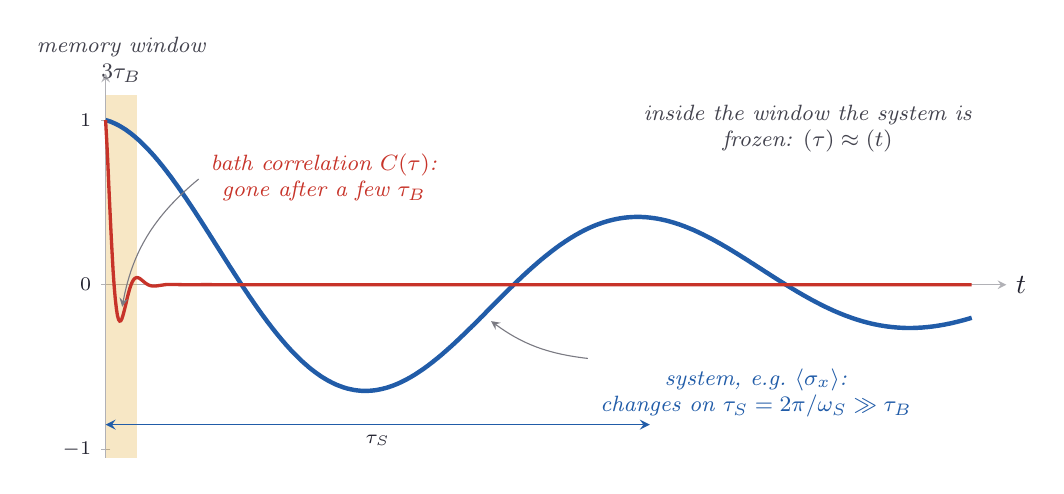
\begin{tikzpicture}[ink/.style={line width=0.9pt, ndInk}, faint/.style={line width=0.4pt, ndInk!35}, dashedink/.style={line width=0.5pt, ndInk!55, dash pattern=on 2.5pt off 2pt}, vec/.style={->, >=stealth, line width=1.2pt}, note/.style={font=\footnotesize\itshape, text=ndInk!85, align=center}, pointer/.style={->, >=stealth, line width=0.4pt, ndInk!60, shorten >=2pt, shorten <=1pt}, dot/.style={circle, fill=ndInk, inner sep=0pt, minimum size=3.4pt}, wash/.style={fill=ndSky, fill opacity=0.55}, every node/.style={text=ndInk}]
\definecolor{ndInk}{rgb}{0.13,0.13,0.18}
\definecolor{ndPaper}{rgb}{0.99,0.96,0.88}
\definecolor{ndSky}{rgb}{0.84,0.91,0.98}
\definecolor{ndRose}{rgb}{0.98,0.86,0.84}
\definecolor{ndBlue}{rgb}{0.13,0.36,0.66}
\definecolor{ndRed}{rgb}{0.78,0.20,0.16}
\definecolor{ndGold}{rgb}{0.88,0.62,0.10}
\definecolor{ndGreen}{rgb}{0.18,0.52,0.30}
\draw[faint, ->, >=stealth] (0.000,2.195) -- (11.440,2.195) node[right, text=ndInk] {$t$};
\draw[faint, ->, >=stealth] (0.000,0.000) -- (0.000,4.876) node[above, text=ndInk] {};
\draw[faint] (0.060,0.105) -- (-0.060,0.105) node[left, font=\scriptsize, text=ndInk] {$-1$};
\draw[faint] (0.060,2.195) -- (-0.060,2.195) node[left, font=\scriptsize, text=ndInk] {$0$};
\draw[faint] (0.060,4.286) -- (-0.060,4.286) node[left, font=\scriptsize, text=ndInk] {$1$};
\fill[ndGold, fill opacity=0.25] (0.000,0.000) rectangle (0.396,4.600);
\draw[line width=1.6pt, ndBlue] (0.000,4.286) -- (0.014,4.282) -- (0.028,4.278) -- (0.041,4.274) -- (0.055,4.269) -- (0.069,4.264) -- (0.083,4.258) -- (0.096,4.252) -- (0.110,4.246) -- (0.124,4.240) -- (0.138,4.233) -- (0.151,4.226) -- (0.165,4.219) -- (0.179,4.211) -- (0.193,4.203) -- (0.207,4.195) -- (0.220,4.187) -- (0.234,4.178) -- (0.248,4.169) -- (0.262,4.160) -- (0.275,4.150) -- (0.289,4.140) -- (0.303,4.130) -- (0.317,4.120) -- (0.330,4.109) -- (0.344,4.098) -- (0.358,4.087) -- (0.372,4.075) -- (0.385,4.063) -- (0.399,4.051) -- (0.413,4.039) -- (0.427,4.027) -- (0.441,4.014) -- (0.454,4.001) -- (0.468,3.988) -- (0.482,3.974) -- (0.496,3.960) -- (0.509,3.946) -- (0.523,3.932) -- (0.537,3.918) -- (0.551,3.903) -- (0.564,3.888) -- (0.578,3.873) -- (0.592,3.858) -- (0.606,3.842) -- (0.620,3.827) -- (0.633,3.811) -- (0.647,3.795) -- (0.661,3.778) -- (0.675,3.762) -- (0.688,3.745) -- (0.702,3.728) -- (0.716,3.711) -- (0.730,3.694) -- (0.743,3.677) -- (0.757,3.659) -- (0.771,3.641) -- (0.785,3.623) -- (0.798,3.605) -- (0.812,3.587) -- (0.826,3.569) -- (0.840,3.550) -- (0.854,3.531) -- (0.867,3.512) -- (0.881,3.493) -- (0.895,3.474) -- (0.909,3.455) -- (0.922,3.436) -- (0.936,3.416) -- (0.950,3.396) -- (0.964,3.376) -- (0.977,3.357) -- (0.991,3.337) -- (1.005,3.316) -- (1.019,3.296) -- (1.033,3.276) -- (1.046,3.255) -- (1.060,3.235) -- (1.074,3.214) -- (1.088,3.194) -- (1.101,3.173) -- (1.115,3.152) -- (1.129,3.131) -- (1.143,3.110) -- (1.156,3.089) -- (1.170,3.068) -- (1.184,3.046) -- (1.198,3.025) -- (1.212,3.004) -- (1.225,2.982) -- (1.239,2.961) -- (1.253,2.939) -- (1.267,2.918) -- (1.280,2.896) -- (1.294,2.874) -- (1.308,2.853) -- (1.322,2.831) -- (1.335,2.809) -- (1.349,2.788) -- (1.363,2.766) -- (1.377,2.744) -- (1.390,2.722) -- (1.404,2.701) -- (1.418,2.679) -- (1.432,2.657) -- (1.446,2.635) -- (1.459,2.614) -- (1.473,2.592) -- (1.487,2.570) -- (1.501,2.548) -- (1.514,2.527) -- (1.528,2.505) -- (1.542,2.483) -- (1.556,2.462) -- (1.569,2.440) -- (1.583,2.419) -- (1.597,2.397) -- (1.611,2.376) -- (1.625,2.354) -- (1.638,2.333) -- (1.652,2.312) -- (1.666,2.290) -- (1.680,2.269) -- (1.693,2.248) -- (1.707,2.227) -- (1.721,2.206) -- (1.735,2.185) -- (1.748,2.164) -- (1.762,2.144) -- (1.776,2.123) -- (1.790,2.102) -- (1.804,2.082) -- (1.817,2.061) -- (1.831,2.041) -- (1.845,2.021) -- (1.859,2.001) -- (1.872,1.981) -- (1.886,1.961) -- (1.900,1.941) -- (1.914,1.921) -- (1.927,1.902) -- (1.941,1.882) -- (1.955,1.863) -- (1.969,1.844) -- (1.982,1.825) -- (1.996,1.806) -- (2.010,1.787) -- (2.024,1.768) -- (2.038,1.750) -- (2.051,1.731) -- (2.065,1.713) -- (2.079,1.695) -- (2.093,1.677) -- (2.106,1.659) -- (2.120,1.641) -- (2.134,1.624) -- (2.148,1.606) -- (2.161,1.589) -- (2.175,1.572) -- (2.189,1.555) -- (2.203,1.538) -- (2.217,1.522) -- (2.230,1.505) -- (2.244,1.489) -- (2.258,1.473) -- (2.272,1.457) -- (2.285,1.441) -- (2.299,1.426) -- (2.313,1.410) -- (2.327,1.395) -- (2.340,1.380) -- (2.354,1.365) -- (2.368,1.351) -- (2.382,1.336) -- (2.395,1.322) -- (2.409,1.308) -- (2.423,1.294) -- (2.437,1.280) -- (2.451,1.267) -- (2.464,1.253) -- (2.478,1.240) -- (2.492,1.227) -- (2.506,1.214) -- (2.519,1.202) -- (2.533,1.190) -- (2.547,1.178) -- (2.561,1.166) -- (2.574,1.154) -- (2.588,1.142) -- (2.602,1.131) -- (2.616,1.120) -- (2.630,1.109) -- (2.643,1.099) -- (2.657,1.088) -- (2.671,1.078) -- (2.685,1.068) -- (2.698,1.058) -- (2.712,1.049) -- (2.726,1.039) -- (2.740,1.030) -- (2.753,1.021) -- (2.767,1.013) -- (2.781,1.004) -- (2.795,0.996) -- (2.809,0.988) -- (2.822,0.980) -- (2.836,0.972) -- (2.850,0.965) -- (2.864,0.958) -- (2.877,0.951) -- (2.891,0.944) -- (2.905,0.938) -- (2.919,0.931) -- (2.932,0.925) -- (2.946,0.920) -- (2.960,0.914) -- (2.974,0.909) -- (2.987,0.904) -- (3.001,0.899) -- (3.015,0.894) -- (3.029,0.889) -- (3.043,0.885) -- (3.056,0.881) -- (3.070,0.877) -- (3.084,0.874) -- (3.098,0.871) -- (3.111,0.867) -- (3.125,0.865) -- (3.139,0.862) -- (3.153,0.859) -- (3.166,0.857) -- (3.180,0.855) -- (3.194,0.853) -- (3.208,0.852) -- (3.222,0.850) -- (3.235,0.849) -- (3.249,0.848) -- (3.263,0.848) -- (3.277,0.847) -- (3.290,0.847) -- (3.304,0.847) -- (3.318,0.847) -- (3.332,0.848) -- (3.345,0.848) -- (3.359,0.849) -- (3.373,0.850) -- (3.387,0.851) -- (3.401,0.853) -- (3.414,0.854) -- (3.428,0.856) -- (3.442,0.858) -- (3.456,0.861) -- (3.469,0.863) -- (3.483,0.866) -- (3.497,0.869) -- (3.511,0.872) -- (3.524,0.875) -- (3.538,0.879) -- (3.552,0.882) -- (3.566,0.886) -- (3.579,0.890) -- (3.593,0.894) -- (3.607,0.899) -- (3.621,0.904) -- (3.635,0.908) -- (3.648,0.913) -- (3.662,0.919) -- (3.676,0.924) -- (3.690,0.930) -- (3.703,0.935) -- (3.717,0.941) -- (3.731,0.948) -- (3.745,0.954) -- (3.758,0.960) -- (3.772,0.967) -- (3.786,0.974) -- (3.800,0.981) -- (3.814,0.988) -- (3.827,0.995) -- (3.841,1.003) -- (3.855,1.011) -- (3.869,1.018) -- (3.882,1.026) -- (3.896,1.035) -- (3.910,1.043) -- (3.924,1.051) -- (3.937,1.060) -- (3.951,1.069) -- (3.965,1.078) -- (3.979,1.087) -- (3.992,1.096) -- (4.006,1.105) -- (4.020,1.115) -- (4.034,1.124) -- (4.048,1.134) -- (4.061,1.144) -- (4.075,1.154) -- (4.089,1.164) -- (4.103,1.174) -- (4.116,1.185) -- (4.130,1.195) -- (4.144,1.206) -- (4.158,1.217) -- (4.171,1.228) -- (4.185,1.239) -- (4.199,1.250) -- (4.213,1.261) -- (4.227,1.272) -- (4.240,1.284) -- (4.254,1.295) -- (4.268,1.307) -- (4.282,1.319) -- (4.295,1.331) -- (4.309,1.343) -- (4.323,1.355) -- (4.337,1.367) -- (4.350,1.379) -- (4.364,1.391) -- (4.378,1.404) -- (4.392,1.416) -- (4.406,1.429) -- (4.419,1.441) -- (4.433,1.454) -- (4.447,1.467) -- (4.461,1.480) -- (4.474,1.493) -- (4.488,1.506) -- (4.502,1.519) -- (4.516,1.532) -- (4.529,1.545) -- (4.543,1.558) -- (4.557,1.571) -- (4.571,1.585) -- (4.584,1.598) -- (4.598,1.612) -- (4.612,1.625) -- (4.626,1.639) -- (4.640,1.652) -- (4.653,1.666) -- (4.667,1.679) -- (4.681,1.693) -- (4.695,1.707) -- (4.708,1.720) -- (4.722,1.734) -- (4.736,1.748) -- (4.750,1.762) -- (4.763,1.776) -- (4.777,1.789) -- (4.791,1.803) -- (4.805,1.817) -- (4.819,1.831) -- (4.832,1.845) -- (4.846,1.859) -- (4.860,1.873) -- (4.874,1.887) -- (4.887,1.901) -- (4.901,1.914) -- (4.915,1.928) -- (4.929,1.942) -- (4.942,1.956) -- (4.956,1.970) -- (4.970,1.984) -- (4.984,1.998) -- (4.997,2.011) -- (5.011,2.025) -- (5.025,2.039) -- (5.039,2.053) -- (5.053,2.067) -- (5.066,2.080) -- (5.080,2.094) -- (5.094,2.108) -- (5.108,2.121) -- (5.121,2.135) -- (5.135,2.148) -- (5.149,2.162) -- (5.163,2.175) -- (5.176,2.189) -- (5.190,2.202) -- (5.204,2.215) -- (5.218,2.228) -- (5.232,2.242) -- (5.245,2.255) -- (5.259,2.268) -- (5.273,2.281) -- (5.287,2.294) -- (5.300,2.307) -- (5.314,2.320) -- (5.328,2.332) -- (5.342,2.345) -- (5.355,2.358) -- (5.369,2.370) -- (5.383,2.383) -- (5.397,2.395) -- (5.411,2.408) -- (5.424,2.420) -- (5.438,2.432) -- (5.452,2.444) -- (5.466,2.456) -- (5.479,2.468) -- (5.493,2.480) -- (5.507,2.492) -- (5.521,2.503) -- (5.534,2.515) -- (5.548,2.526) -- (5.562,2.538) -- (5.576,2.549) -- (5.589,2.560) -- (5.603,2.571) -- (5.617,2.582) -- (5.631,2.593) -- (5.645,2.604) -- (5.658,2.615) -- (5.672,2.625) -- (5.686,2.636) -- (5.700,2.646) -- (5.713,2.657) -- (5.727,2.667) -- (5.741,2.677) -- (5.755,2.687) -- (5.768,2.697) -- (5.782,2.706) -- (5.796,2.716) -- (5.810,2.725) -- (5.824,2.735) -- (5.837,2.744) -- (5.851,2.753) -- (5.865,2.762) -- (5.879,2.771) -- (5.892,2.780) -- (5.906,2.788) -- (5.920,2.797) -- (5.934,2.805) -- (5.947,2.813) -- (5.961,2.822) -- (5.975,2.830) -- (5.989,2.837) -- (6.003,2.845) -- (6.016,2.853) -- (6.030,2.860) -- (6.044,2.868) -- (6.058,2.875) -- (6.071,2.882) -- (6.085,2.889) -- (6.099,2.896) -- (6.113,2.902) -- (6.126,2.909) -- (6.140,2.915) -- (6.154,2.921) -- (6.168,2.928) -- (6.181,2.933) -- (6.195,2.939) -- (6.209,2.945) -- (6.223,2.951) -- (6.237,2.956) -- (6.250,2.961) -- (6.264,2.966) -- (6.278,2.971) -- (6.292,2.976) -- (6.305,2.981) -- (6.319,2.985) -- (6.333,2.990) -- (6.347,2.994) -- (6.360,2.998) -- (6.374,3.002) -- (6.388,3.006) -- (6.402,3.010) -- (6.416,3.013) -- (6.429,3.017) -- (6.443,3.020) -- (6.457,3.023) -- (6.471,3.026) -- (6.484,3.029) -- (6.498,3.032) -- (6.512,3.034) -- (6.526,3.037) -- (6.539,3.039) -- (6.553,3.041) -- (6.567,3.043) -- (6.581,3.045) -- (6.594,3.047) -- (6.608,3.048) -- (6.622,3.050) -- (6.636,3.051) -- (6.650,3.052) -- (6.663,3.053) -- (6.677,3.054) -- (6.691,3.055) -- (6.705,3.055) -- (6.718,3.056) -- (6.732,3.056) -- (6.746,3.056) -- (6.760,3.056) -- (6.773,3.056) -- (6.787,3.056) -- (6.801,3.056) -- (6.815,3.055) -- (6.829,3.054) -- (6.842,3.054) -- (6.856,3.053) -- (6.870,3.052) -- (6.884,3.050) -- (6.897,3.049) -- (6.911,3.048) -- (6.925,3.046) -- (6.939,3.044) -- (6.952,3.042) -- (6.966,3.041) -- (6.980,3.038) -- (6.994,3.036) -- (7.008,3.034) -- (7.021,3.031) -- (7.035,3.029) -- (7.049,3.026) -- (7.063,3.023) -- (7.076,3.020) -- (7.090,3.017) -- (7.104,3.014) -- (7.118,3.011) -- (7.131,3.007) -- (7.145,3.004) -- (7.159,3.000) -- (7.173,2.996) -- (7.186,2.992) -- (7.200,2.988) -- (7.214,2.984) -- (7.228,2.980) -- (7.242,2.975) -- (7.255,2.971) -- (7.269,2.966) -- (7.283,2.962) -- (7.297,2.957) -- (7.310,2.952) -- (7.324,2.947) -- (7.338,2.942) -- (7.352,2.937) -- (7.365,2.931) -- (7.379,2.926) -- (7.393,2.920) -- (7.407,2.915) -- (7.421,2.909) -- (7.434,2.903) -- (7.448,2.898) -- (7.462,2.892) -- (7.476,2.886) -- (7.489,2.879) -- (7.503,2.873) -- (7.517,2.867) -- (7.531,2.860) -- (7.544,2.854) -- (7.558,2.847) -- (7.572,2.841) -- (7.586,2.834) -- (7.599,2.827) -- (7.613,2.820) -- (7.627,2.813) -- (7.641,2.806) -- (7.655,2.799) -- (7.668,2.792) -- (7.682,2.785) -- (7.696,2.778) -- (7.710,2.770) -- (7.723,2.763) -- (7.737,2.755) -- (7.751,2.748) -- (7.765,2.740) -- (7.778,2.732) -- (7.792,2.725) -- (7.806,2.717) -- (7.820,2.709) -- (7.834,2.701) -- (7.847,2.693) -- (7.861,2.685) -- (7.875,2.677) -- (7.889,2.669) -- (7.902,2.661) -- (7.916,2.653) -- (7.930,2.644) -- (7.944,2.636) -- (7.957,2.628) -- (7.971,2.619) -- (7.985,2.611) -- (7.999,2.602) -- (8.013,2.594) -- (8.026,2.585) -- (8.040,2.577) -- (8.054,2.568) -- (8.068,2.560) -- (8.081,2.551) -- (8.095,2.542) -- (8.109,2.534) -- (8.123,2.525) -- (8.136,2.516) -- (8.150,2.508) -- (8.164,2.499) -- (8.178,2.490) -- (8.191,2.481) -- (8.205,2.472) -- (8.219,2.464) -- (8.233,2.455) -- (8.247,2.446) -- (8.260,2.437) -- (8.274,2.428) -- (8.288,2.419) -- (8.302,2.410) -- (8.315,2.402) -- (8.329,2.393) -- (8.343,2.384) -- (8.357,2.375) -- (8.370,2.366) -- (8.384,2.357) -- (8.398,2.348) -- (8.412,2.340) -- (8.426,2.331) -- (8.439,2.322) -- (8.453,2.313) -- (8.467,2.304) -- (8.481,2.295) -- (8.494,2.287) -- (8.508,2.278) -- (8.522,2.269) -- (8.536,2.260) -- (8.549,2.252) -- (8.563,2.243) -- (8.577,2.234) -- (8.591,2.226) -- (8.605,2.217) -- (8.618,2.209) -- (8.632,2.200) -- (8.646,2.191) -- (8.660,2.183) -- (8.673,2.175) -- (8.687,2.166) -- (8.701,2.158) -- (8.715,2.149) -- (8.728,2.141) -- (8.742,2.133) -- (8.756,2.125) -- (8.770,2.116) -- (8.783,2.108) -- (8.797,2.100) -- (8.811,2.092) -- (8.825,2.084) -- (8.839,2.076) -- (8.852,2.068) -- (8.866,2.060) -- (8.880,2.052) -- (8.894,2.045) -- (8.907,2.037) -- (8.921,2.029) -- (8.935,2.022) -- (8.949,2.014) -- (8.962,2.006) -- (8.976,1.999) -- (8.990,1.992) -- (9.004,1.984) -- (9.018,1.977) -- (9.031,1.970) -- (9.045,1.963) -- (9.059,1.956) -- (9.073,1.948) -- (9.086,1.942) -- (9.100,1.935) -- (9.114,1.928) -- (9.128,1.921) -- (9.141,1.914) -- (9.155,1.908) -- (9.169,1.901) -- (9.183,1.895) -- (9.196,1.888) -- (9.210,1.882) -- (9.224,1.876) -- (9.238,1.869) -- (9.252,1.863) -- (9.265,1.857) -- (9.279,1.851) -- (9.293,1.845) -- (9.307,1.840) -- (9.320,1.834) -- (9.334,1.828) -- (9.348,1.823) -- (9.362,1.817) -- (9.375,1.812) -- (9.389,1.806) -- (9.403,1.801) -- (9.417,1.796) -- (9.431,1.791) -- (9.444,1.786) -- (9.458,1.781) -- (9.472,1.776) -- (9.486,1.771) -- (9.499,1.766) -- (9.513,1.762) -- (9.527,1.757) -- (9.541,1.753) -- (9.554,1.749) -- (9.568,1.744) -- (9.582,1.740) -- (9.596,1.736) -- (9.610,1.732) -- (9.623,1.728) -- (9.637,1.724) -- (9.651,1.721) -- (9.665,1.717) -- (9.678,1.713) -- (9.692,1.710) -- (9.706,1.707) -- (9.720,1.703) -- (9.733,1.700) -- (9.747,1.697) -- (9.761,1.694) -- (9.775,1.691) -- (9.788,1.688) -- (9.802,1.686) -- (9.816,1.683) -- (9.830,1.680) -- (9.844,1.678) -- (9.857,1.676) -- (9.871,1.673) -- (9.885,1.671) -- (9.899,1.669) -- (9.912,1.667) -- (9.926,1.665) -- (9.940,1.663) -- (9.954,1.662) -- (9.967,1.660) -- (9.981,1.658) -- (9.995,1.657) -- (10.009,1.656) -- (10.023,1.654) -- (10.036,1.653) -- (10.050,1.652) -- (10.064,1.651) -- (10.078,1.650) -- (10.091,1.649) -- (10.105,1.649) -- (10.119,1.648) -- (10.133,1.647) -- (10.146,1.647) -- (10.160,1.646) -- (10.174,1.646) -- (10.188,1.646) -- (10.202,1.646) -- (10.215,1.646) -- (10.229,1.646) -- (10.243,1.646) -- (10.257,1.646) -- (10.270,1.647) -- (10.284,1.647) -- (10.298,1.648) -- (10.312,1.648) -- (10.325,1.649) -- (10.339,1.650) -- (10.353,1.650) -- (10.367,1.651) -- (10.380,1.652) -- (10.394,1.654) -- (10.408,1.655) -- (10.422,1.656) -- (10.436,1.657) -- (10.449,1.659) -- (10.463,1.660) -- (10.477,1.662) -- (10.491,1.663) -- (10.504,1.665) -- (10.518,1.667) -- (10.532,1.669) -- (10.546,1.671) -- (10.559,1.673) -- (10.573,1.675) -- (10.587,1.677) -- (10.601,1.680) -- (10.615,1.682) -- (10.628,1.684) -- (10.642,1.687) -- (10.656,1.689) -- (10.670,1.692) -- (10.683,1.695) -- (10.697,1.698) -- (10.711,1.700) -- (10.725,1.703) -- (10.738,1.706) -- (10.752,1.709) -- (10.766,1.712) -- (10.780,1.716) -- (10.793,1.719) -- (10.807,1.722) -- (10.821,1.726) -- (10.835,1.729) -- (10.849,1.733) -- (10.862,1.736) -- (10.876,1.740) -- (10.890,1.743) -- (10.904,1.747) -- (10.917,1.751) -- (10.931,1.755) -- (10.945,1.759) -- (10.959,1.763) -- (10.972,1.767) -- (10.986,1.771) -- (11.000,1.775);
\draw[line width=1.2pt, ndRed] (0.000,4.286) -- (0.014,4.042) -- (0.028,3.758) -- (0.041,3.457) -- (0.055,3.154) -- (0.069,2.865) -- (0.083,2.599) -- (0.096,2.365) -- (0.110,2.167) -- (0.124,2.008) -- (0.138,1.887) -- (0.151,1.803) -- (0.165,1.753) -- (0.179,1.733) -- (0.193,1.737) -- (0.207,1.762) -- (0.220,1.802) -- (0.234,1.853) -- (0.248,1.909) -- (0.262,1.968) -- (0.275,2.027) -- (0.289,2.082) -- (0.303,2.132) -- (0.317,2.175) -- (0.330,2.211) -- (0.344,2.240) -- (0.358,2.261) -- (0.372,2.276) -- (0.385,2.283) -- (0.399,2.286) -- (0.413,2.284) -- (0.427,2.278) -- (0.441,2.269) -- (0.454,2.259) -- (0.468,2.248) -- (0.482,2.236) -- (0.496,2.225) -- (0.509,2.214) -- (0.523,2.205) -- (0.537,2.197) -- (0.551,2.190) -- (0.564,2.185) -- (0.578,2.182) -- (0.592,2.179) -- (0.606,2.178) -- (0.620,2.178) -- (0.633,2.179) -- (0.647,2.180) -- (0.661,2.182) -- (0.675,2.184) -- (0.688,2.186) -- (0.702,2.188) -- (0.716,2.190) -- (0.730,2.192) -- (0.743,2.194) -- (0.757,2.196) -- (0.771,2.197) -- (0.785,2.198) -- (0.798,2.198) -- (0.812,2.199) -- (0.826,2.199) -- (0.840,2.199) -- (0.854,2.199) -- (0.867,2.198) -- (0.881,2.198) -- (0.895,2.198) -- (0.909,2.197) -- (0.922,2.197) -- (0.936,2.196) -- (0.950,2.196) -- (0.964,2.196) -- (0.977,2.195) -- (0.991,2.195) -- (1.005,2.195) -- (1.019,2.195) -- (1.033,2.195) -- (1.046,2.195) -- (1.060,2.195) -- (1.074,2.195) -- (1.088,2.195) -- (1.101,2.195) -- (1.115,2.195) -- (1.129,2.195) -- (1.143,2.195) -- (1.156,2.195) -- (1.170,2.195) -- (1.184,2.195) -- (1.198,2.195) -- (1.212,2.196) -- (1.225,2.196) -- (1.239,2.196) -- (1.253,2.196) -- (1.267,2.196) -- (1.280,2.196) -- (1.294,2.196) -- (1.308,2.196) -- (1.322,2.196) -- (1.335,2.196) -- (1.349,2.196) -- (1.363,2.195) -- (1.377,2.195) -- (1.390,2.195) -- (1.404,2.195) -- (1.418,2.195) -- (1.432,2.195) -- (1.446,2.195) -- (1.459,2.195) -- (1.473,2.195) -- (1.487,2.195) -- (1.501,2.195) -- (1.514,2.195) -- (1.528,2.195) -- (1.542,2.195) -- (1.556,2.195) -- (1.569,2.195) -- (1.583,2.195) -- (1.597,2.195) -- (1.611,2.195) -- (1.625,2.195) -- (1.638,2.195) -- (1.652,2.195) -- (1.666,2.195) -- (1.680,2.195) -- (1.693,2.195) -- (1.707,2.195) -- (1.721,2.195) -- (1.735,2.195) -- (1.748,2.195) -- (1.762,2.195) -- (1.776,2.195) -- (1.790,2.195) -- (1.804,2.195) -- (1.817,2.195) -- (1.831,2.195) -- (1.845,2.195) -- (1.859,2.195) -- (1.872,2.195) -- (1.886,2.195) -- (1.900,2.195) -- (1.914,2.195) -- (1.927,2.195) -- (1.941,2.195) -- (1.955,2.195) -- (1.969,2.195) -- (1.982,2.195) -- (1.996,2.195) -- (2.010,2.195) -- (2.024,2.195) -- (2.038,2.195) -- (2.051,2.195) -- (2.065,2.195) -- (2.079,2.195) -- (2.093,2.195) -- (2.106,2.195) -- (2.120,2.195) -- (2.134,2.195) -- (2.148,2.195) -- (2.161,2.195) -- (2.175,2.195) -- (2.189,2.195) -- (2.203,2.195) -- (2.217,2.195) -- (2.230,2.195) -- (2.244,2.195) -- (2.258,2.195) -- (2.272,2.195) -- (2.285,2.195) -- (2.299,2.195) -- (2.313,2.195) -- (2.327,2.195) -- (2.340,2.195) -- (2.354,2.195) -- (2.368,2.195) -- (2.382,2.195) -- (2.395,2.195) -- (2.409,2.195) -- (2.423,2.195) -- (2.437,2.195) -- (2.451,2.195) -- (2.464,2.195) -- (2.478,2.195) -- (2.492,2.195) -- (2.506,2.195) -- (2.519,2.195) -- (2.533,2.195) -- (2.547,2.195) -- (2.561,2.195) -- (2.574,2.195) -- (2.588,2.195) -- (2.602,2.195) -- (2.616,2.195) -- (2.630,2.195) -- (2.643,2.195) -- (2.657,2.195) -- (2.671,2.195) -- (2.685,2.195) -- (2.698,2.195) -- (2.712,2.195) -- (2.726,2.195) -- (2.740,2.195) -- (2.753,2.195) -- (2.767,2.195) -- (2.781,2.195) -- (2.795,2.195) -- (2.809,2.195) -- (2.822,2.195) -- (2.836,2.195) -- (2.850,2.195) -- (2.864,2.195) -- (2.877,2.195) -- (2.891,2.195) -- (2.905,2.195) -- (2.919,2.195) -- (2.932,2.195) -- (2.946,2.195) -- (2.960,2.195) -- (2.974,2.195) -- (2.987,2.195) -- (3.001,2.195) -- (3.015,2.195) -- (3.029,2.195) -- (3.043,2.195) -- (3.056,2.195) -- (3.070,2.195) -- (3.084,2.195) -- (3.098,2.195) -- (3.111,2.195) -- (3.125,2.195) -- (3.139,2.195) -- (3.153,2.195) -- (3.166,2.195) -- (3.180,2.195) -- (3.194,2.195) -- (3.208,2.195) -- (3.222,2.195) -- (3.235,2.195) -- (3.249,2.195) -- (3.263,2.195) -- (3.277,2.195) -- (3.290,2.195) -- (3.304,2.195) -- (3.318,2.195) -- (3.332,2.195) -- (3.345,2.195) -- (3.359,2.195) -- (3.373,2.195) -- (3.387,2.195) -- (3.401,2.195) -- (3.414,2.195) -- (3.428,2.195) -- (3.442,2.195) -- (3.456,2.195) -- (3.469,2.195) -- (3.483,2.195) -- (3.497,2.195) -- (3.511,2.195) -- (3.524,2.195) -- (3.538,2.195) -- (3.552,2.195) -- (3.566,2.195) -- (3.579,2.195) -- (3.593,2.195) -- (3.607,2.195) -- (3.621,2.195) -- (3.635,2.195) -- (3.648,2.195) -- (3.662,2.195) -- (3.676,2.195) -- (3.690,2.195) -- (3.703,2.195) -- (3.717,2.195) -- (3.731,2.195) -- (3.745,2.195) -- (3.758,2.195) -- (3.772,2.195) -- (3.786,2.195) -- (3.800,2.195) -- (3.814,2.195) -- (3.827,2.195) -- (3.841,2.195) -- (3.855,2.195) -- (3.869,2.195) -- (3.882,2.195) -- (3.896,2.195) -- (3.910,2.195) -- (3.924,2.195) -- (3.937,2.195) -- (3.951,2.195) -- (3.965,2.195) -- (3.979,2.195) -- (3.992,2.195) -- (4.006,2.195) -- (4.020,2.195) -- (4.034,2.195) -- (4.048,2.195) -- (4.061,2.195) -- (4.075,2.195) -- (4.089,2.195) -- (4.103,2.195) -- (4.116,2.195) -- (4.130,2.195) -- (4.144,2.195) -- (4.158,2.195) -- (4.171,2.195) -- (4.185,2.195) -- (4.199,2.195) -- (4.213,2.195) -- (4.227,2.195) -- (4.240,2.195) -- (4.254,2.195) -- (4.268,2.195) -- (4.282,2.195) -- (4.295,2.195) -- (4.309,2.195) -- (4.323,2.195) -- (4.337,2.195) -- (4.350,2.195) -- (4.364,2.195) -- (4.378,2.195) -- (4.392,2.195) -- (4.406,2.195) -- (4.419,2.195) -- (4.433,2.195) -- (4.447,2.195) -- (4.461,2.195) -- (4.474,2.195) -- (4.488,2.195) -- (4.502,2.195) -- (4.516,2.195) -- (4.529,2.195) -- (4.543,2.195) -- (4.557,2.195) -- (4.571,2.195) -- (4.584,2.195) -- (4.598,2.195) -- (4.612,2.195) -- (4.626,2.195) -- (4.640,2.195) -- (4.653,2.195) -- (4.667,2.195) -- (4.681,2.195) -- (4.695,2.195) -- (4.708,2.195) -- (4.722,2.195) -- (4.736,2.195) -- (4.750,2.195) -- (4.763,2.195) -- (4.777,2.195) -- (4.791,2.195) -- (4.805,2.195) -- (4.819,2.195) -- (4.832,2.195) -- (4.846,2.195) -- (4.860,2.195) -- (4.874,2.195) -- (4.887,2.195) -- (4.901,2.195) -- (4.915,2.195) -- (4.929,2.195) -- (4.942,2.195) -- (4.956,2.195) -- (4.970,2.195) -- (4.984,2.195) -- (4.997,2.195) -- (5.011,2.195) -- (5.025,2.195) -- (5.039,2.195) -- (5.053,2.195) -- (5.066,2.195) -- (5.080,2.195) -- (5.094,2.195) -- (5.108,2.195) -- (5.121,2.195) -- (5.135,2.195) -- (5.149,2.195) -- (5.163,2.195) -- (5.176,2.195) -- (5.190,2.195) -- (5.204,2.195) -- (5.218,2.195) -- (5.232,2.195) -- (5.245,2.195) -- (5.259,2.195) -- (5.273,2.195) -- (5.287,2.195) -- (5.300,2.195) -- (5.314,2.195) -- (5.328,2.195) -- (5.342,2.195) -- (5.355,2.195) -- (5.369,2.195) -- (5.383,2.195) -- (5.397,2.195) -- (5.411,2.195) -- (5.424,2.195) -- (5.438,2.195) -- (5.452,2.195) -- (5.466,2.195) -- (5.479,2.195) -- (5.493,2.195) -- (5.507,2.195) -- (5.521,2.195) -- (5.534,2.195) -- (5.548,2.195) -- (5.562,2.195) -- (5.576,2.195) -- (5.589,2.195) -- (5.603,2.195) -- (5.617,2.195) -- (5.631,2.195) -- (5.645,2.195) -- (5.658,2.195) -- (5.672,2.195) -- (5.686,2.195) -- (5.700,2.195) -- (5.713,2.195) -- (5.727,2.195) -- (5.741,2.195) -- (5.755,2.195) -- (5.768,2.195) -- (5.782,2.195) -- (5.796,2.195) -- (5.810,2.195) -- (5.824,2.195) -- (5.837,2.195) -- (5.851,2.195) -- (5.865,2.195) -- (5.879,2.195) -- (5.892,2.195) -- (5.906,2.195) -- (5.920,2.195) -- (5.934,2.195) -- (5.947,2.195) -- (5.961,2.195) -- (5.975,2.195) -- (5.989,2.195) -- (6.003,2.195) -- (6.016,2.195) -- (6.030,2.195) -- (6.044,2.195) -- (6.058,2.195) -- (6.071,2.195) -- (6.085,2.195) -- (6.099,2.195) -- (6.113,2.195) -- (6.126,2.195) -- (6.140,2.195) -- (6.154,2.195) -- (6.168,2.195) -- (6.181,2.195) -- (6.195,2.195) -- (6.209,2.195) -- (6.223,2.195) -- (6.237,2.195) -- (6.250,2.195) -- (6.264,2.195) -- (6.278,2.195) -- (6.292,2.195) -- (6.305,2.195) -- (6.319,2.195) -- (6.333,2.195) -- (6.347,2.195) -- (6.360,2.195) -- (6.374,2.195) -- (6.388,2.195) -- (6.402,2.195) -- (6.416,2.195) -- (6.429,2.195) -- (6.443,2.195) -- (6.457,2.195) -- (6.471,2.195) -- (6.484,2.195) -- (6.498,2.195) -- (6.512,2.195) -- (6.526,2.195) -- (6.539,2.195) -- (6.553,2.195) -- (6.567,2.195) -- (6.581,2.195) -- (6.594,2.195) -- (6.608,2.195) -- (6.622,2.195) -- (6.636,2.195) -- (6.650,2.195) -- (6.663,2.195) -- (6.677,2.195) -- (6.691,2.195) -- (6.705,2.195) -- (6.718,2.195) -- (6.732,2.195) -- (6.746,2.195) -- (6.760,2.195) -- (6.773,2.195) -- (6.787,2.195) -- (6.801,2.195) -- (6.815,2.195) -- (6.829,2.195) -- (6.842,2.195) -- (6.856,2.195) -- (6.870,2.195) -- (6.884,2.195) -- (6.897,2.195) -- (6.911,2.195) -- (6.925,2.195) -- (6.939,2.195) -- (6.952,2.195) -- (6.966,2.195) -- (6.980,2.195) -- (6.994,2.195) -- (7.008,2.195) -- (7.021,2.195) -- (7.035,2.195) -- (7.049,2.195) -- (7.063,2.195) -- (7.076,2.195) -- (7.090,2.195) -- (7.104,2.195) -- (7.118,2.195) -- (7.131,2.195) -- (7.145,2.195) -- (7.159,2.195) -- (7.173,2.195) -- (7.186,2.195) -- (7.200,2.195) -- (7.214,2.195) -- (7.228,2.195) -- (7.242,2.195) -- (7.255,2.195) -- (7.269,2.195) -- (7.283,2.195) -- (7.297,2.195) -- (7.310,2.195) -- (7.324,2.195) -- (7.338,2.195) -- (7.352,2.195) -- (7.365,2.195) -- (7.379,2.195) -- (7.393,2.195) -- (7.407,2.195) -- (7.421,2.195) -- (7.434,2.195) -- (7.448,2.195) -- (7.462,2.195) -- (7.476,2.195) -- (7.489,2.195) -- (7.503,2.195) -- (7.517,2.195) -- (7.531,2.195) -- (7.544,2.195) -- (7.558,2.195) -- (7.572,2.195) -- (7.586,2.195) -- (7.599,2.195) -- (7.613,2.195) -- (7.627,2.195) -- (7.641,2.195) -- (7.655,2.195) -- (7.668,2.195) -- (7.682,2.195) -- (7.696,2.195) -- (7.710,2.195) -- (7.723,2.195) -- (7.737,2.195) -- (7.751,2.195) -- (7.765,2.195) -- (7.778,2.195) -- (7.792,2.195) -- (7.806,2.195) -- (7.820,2.195) -- (7.834,2.195) -- (7.847,2.195) -- (7.861,2.195) -- (7.875,2.195) -- (7.889,2.195) -- (7.902,2.195) -- (7.916,2.195) -- (7.930,2.195) -- (7.944,2.195) -- (7.957,2.195) -- (7.971,2.195) -- (7.985,2.195) -- (7.999,2.195) -- (8.013,2.195) -- (8.026,2.195) -- (8.040,2.195) -- (8.054,2.195) -- (8.068,2.195) -- (8.081,2.195) -- (8.095,2.195) -- (8.109,2.195) -- (8.123,2.195) -- (8.136,2.195) -- (8.150,2.195) -- (8.164,2.195) -- (8.178,2.195) -- (8.191,2.195) -- (8.205,2.195) -- (8.219,2.195) -- (8.233,2.195) -- (8.247,2.195) -- (8.260,2.195) -- (8.274,2.195) -- (8.288,2.195) -- (8.302,2.195) -- (8.315,2.195) -- (8.329,2.195) -- (8.343,2.195) -- (8.357,2.195) -- (8.370,2.195) -- (8.384,2.195) -- (8.398,2.195) -- (8.412,2.195) -- (8.426,2.195) -- (8.439,2.195) -- (8.453,2.195) -- (8.467,2.195) -- (8.481,2.195) -- (8.494,2.195) -- (8.508,2.195) -- (8.522,2.195) -- (8.536,2.195) -- (8.549,2.195) -- (8.563,2.195) -- (8.577,2.195) -- (8.591,2.195) -- (8.605,2.195) -- (8.618,2.195) -- (8.632,2.195) -- (8.646,2.195) -- (8.660,2.195) -- (8.673,2.195) -- (8.687,2.195) -- (8.701,2.195) -- (8.715,2.195) -- (8.728,2.195) -- (8.742,2.195) -- (8.756,2.195) -- (8.770,2.195) -- (8.783,2.195) -- (8.797,2.195) -- (8.811,2.195) -- (8.825,2.195) -- (8.839,2.195) -- (8.852,2.195) -- (8.866,2.195) -- (8.880,2.195) -- (8.894,2.195) -- (8.907,2.195) -- (8.921,2.195) -- (8.935,2.195) -- (8.949,2.195) -- (8.962,2.195) -- (8.976,2.195) -- (8.990,2.195) -- (9.004,2.195) -- (9.018,2.195) -- (9.031,2.195) -- (9.045,2.195) -- (9.059,2.195) -- (9.073,2.195) -- (9.086,2.195) -- (9.100,2.195) -- (9.114,2.195) -- (9.128,2.195) -- (9.141,2.195) -- (9.155,2.195) -- (9.169,2.195) -- (9.183,2.195) -- (9.196,2.195) -- (9.210,2.195) -- (9.224,2.195) -- (9.238,2.195) -- (9.252,2.195) -- (9.265,2.195) -- (9.279,2.195) -- (9.293,2.195) -- (9.307,2.195) -- (9.320,2.195) -- (9.334,2.195) -- (9.348,2.195) -- (9.362,2.195) -- (9.375,2.195) -- (9.389,2.195) -- (9.403,2.195) -- (9.417,2.195) -- (9.431,2.195) -- (9.444,2.195) -- (9.458,2.195) -- (9.472,2.195) -- (9.486,2.195) -- (9.499,2.195) -- (9.513,2.195) -- (9.527,2.195) -- (9.541,2.195) -- (9.554,2.195) -- (9.568,2.195) -- (9.582,2.195) -- (9.596,2.195) -- (9.610,2.195) -- (9.623,2.195) -- (9.637,2.195) -- (9.651,2.195) -- (9.665,2.195) -- (9.678,2.195) -- (9.692,2.195) -- (9.706,2.195) -- (9.720,2.195) -- (9.733,2.195) -- (9.747,2.195) -- (9.761,2.195) -- (9.775,2.195) -- (9.788,2.195) -- (9.802,2.195) -- (9.816,2.195) -- (9.830,2.195) -- (9.844,2.195) -- (9.857,2.195) -- (9.871,2.195) -- (9.885,2.195) -- (9.899,2.195) -- (9.912,2.195) -- (9.926,2.195) -- (9.940,2.195) -- (9.954,2.195) -- (9.967,2.195) -- (9.981,2.195) -- (9.995,2.195) -- (10.009,2.195) -- (10.023,2.195) -- (10.036,2.195) -- (10.050,2.195) -- (10.064,2.195) -- (10.078,2.195) -- (10.091,2.195) -- (10.105,2.195) -- (10.119,2.195) -- (10.133,2.195) -- (10.146,2.195) -- (10.160,2.195) -- (10.174,2.195) -- (10.188,2.195) -- (10.202,2.195) -- (10.215,2.195) -- (10.229,2.195) -- (10.243,2.195) -- (10.257,2.195) -- (10.270,2.195) -- (10.284,2.195) -- (10.298,2.195) -- (10.312,2.195) -- (10.325,2.195) -- (10.339,2.195) -- (10.353,2.195) -- (10.367,2.195) -- (10.380,2.195) -- (10.394,2.195) -- (10.408,2.195) -- (10.422,2.195) -- (10.436,2.195) -- (10.449,2.195) -- (10.463,2.195) -- (10.477,2.195) -- (10.491,2.195) -- (10.504,2.195) -- (10.518,2.195) -- (10.532,2.195) -- (10.546,2.195) -- (10.559,2.195) -- (10.573,2.195) -- (10.587,2.195) -- (10.601,2.195) -- (10.615,2.195) -- (10.628,2.195) -- (10.642,2.195) -- (10.656,2.195) -- (10.670,2.195) -- (10.683,2.195) -- (10.697,2.195) -- (10.711,2.195) -- (10.725,2.195) -- (10.738,2.195) -- (10.752,2.195) -- (10.766,2.195) -- (10.780,2.195) -- (10.793,2.195) -- (10.807,2.195) -- (10.821,2.195) -- (10.835,2.195) -- (10.849,2.195) -- (10.862,2.195) -- (10.876,2.195) -- (10.890,2.195) -- (10.904,2.195) -- (10.917,2.195) -- (10.931,2.195) -- (10.945,2.195) -- (10.959,2.195) -- (10.972,2.195) -- (10.986,2.195) -- (11.000,2.195);
\node[note, anchor=south west, text=ndRed] (c) at (1.210,3.136) {bath correlation $C(\tau)$:\\ gone after a few $\tau_B$};
\draw[pointer] (c.west) to[bend right=20] (0.198,1.846);
\node[note, anchor=north west, text=ndBlue] (s) at (6.160,1.255) {system, e.g.\ $\langle\sigma_x\rangle$:\\ changes on $\tau_S=2\pi/\omega_S\gg\tau_B$};
\draw[pointer] (s.north west) to[bend left=15] (4.840,1.775);
\node[note, anchor=south] at (0.198,4.642) {memory window\\ $\lesssim3\tau_B$};
\draw[<->, >=stealth, line width=0.6pt, ndBlue] (0.000,0.418) -- (6.912,0.418) node[midway, below, font=\scriptsize] {$\tau_S$};
\node[note, anchor=west] at (6.710,4.182) {inside the window the system is\\ frozen: $\rhoS(\tau)\approx\rhoS(t)$};
\end{tikzpicture}
}
\caption{A bath correlation function $C(\tau)$ (red) that decays within $\tau_B$, and a system observable (blue) that changes on $\tau_S=2\pi/\omega_S\gg\tau_B$. Within the memory window (shaded) the system is essentially frozen. Generated by \texttt{code/ch03\_timescales.py}.}\label{fig:ch03:timescales}
\end{figure}}
\ona{\endgraf\medskip\noindent\textit{Reading the figure.} The red curve shows how much the environment still ``remembers'' about its own state a time $\tau$ ago; it dies out quickly. The blue curve shows what the system does; it changes slowly. The shaded strip is the stretch of time over which the environment still remembers anything.\endgraf\smallskip\noindent\textit{Why it matters.} This picture is the justification of every memoryless model in this \chap{}. An analogy: the weather can be predicted without tracking individual air molecules, because each molecule forgets its velocity within nanoseconds while the weather changes over hours. In computer-science terms, it is the assumption that a noise process looks like independent (``white'') noise at the timescale of interest. When the two timescales are \emph{not} separated, when the red curve lives as long as the blue one, Markovian models fail, as in Figure~\ref{fig:ch03:nonmarkov} at strong coupling.}
\onp{\begin{center}\resizebox{\linewidth}{!}{% Generated by code/needham.py -- do not edit by hand.
\definecolor{qocA}{rgb}{0.00,0.45,0.70}
\definecolor{qocB}{rgb}{0.90,0.60,0.00}
\definecolor{qocC}{rgb}{0.00,0.62,0.45}
\definecolor{qocD}{rgb}{0.80,0.40,0.00}
\definecolor{qocE}{rgb}{0.80,0.60,0.70}
\definecolor{qocF}{rgb}{0.35,0.70,0.90}
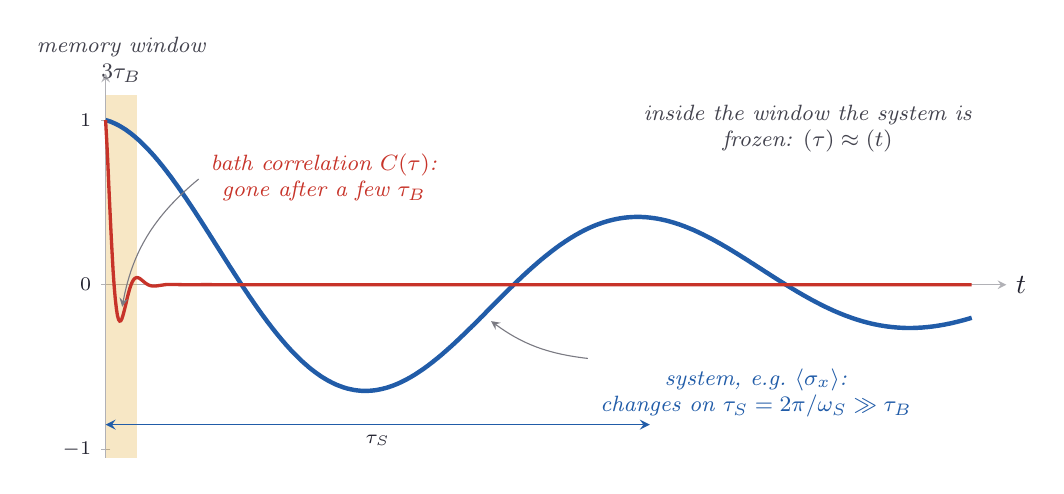
\begin{tikzpicture}[ink/.style={line width=0.9pt, ndInk}, faint/.style={line width=0.4pt, ndInk!35}, dashedink/.style={line width=0.5pt, ndInk!55, dash pattern=on 2.5pt off 2pt}, vec/.style={->, >=stealth, line width=1.2pt}, note/.style={font=\footnotesize\itshape, text=ndInk!85, align=center}, pointer/.style={->, >=stealth, line width=0.4pt, ndInk!60, shorten >=2pt, shorten <=1pt}, dot/.style={circle, fill=ndInk, inner sep=0pt, minimum size=3.4pt}, wash/.style={fill=ndSky, fill opacity=0.55}, every node/.style={text=ndInk}]
\definecolor{ndInk}{rgb}{0.13,0.13,0.18}
\definecolor{ndPaper}{rgb}{0.99,0.96,0.88}
\definecolor{ndSky}{rgb}{0.84,0.91,0.98}
\definecolor{ndRose}{rgb}{0.98,0.86,0.84}
\definecolor{ndBlue}{rgb}{0.13,0.36,0.66}
\definecolor{ndRed}{rgb}{0.78,0.20,0.16}
\definecolor{ndGold}{rgb}{0.88,0.62,0.10}
\definecolor{ndGreen}{rgb}{0.18,0.52,0.30}
\draw[faint, ->, >=stealth] (0.000,2.195) -- (11.440,2.195) node[right, text=ndInk] {$t$};
\draw[faint, ->, >=stealth] (0.000,0.000) -- (0.000,4.876) node[above, text=ndInk] {};
\draw[faint] (0.060,0.105) -- (-0.060,0.105) node[left, font=\scriptsize, text=ndInk] {$-1$};
\draw[faint] (0.060,2.195) -- (-0.060,2.195) node[left, font=\scriptsize, text=ndInk] {$0$};
\draw[faint] (0.060,4.286) -- (-0.060,4.286) node[left, font=\scriptsize, text=ndInk] {$1$};
\fill[ndGold, fill opacity=0.25] (0.000,0.000) rectangle (0.396,4.600);
\draw[line width=1.6pt, ndBlue] (0.000,4.286) -- (0.014,4.282) -- (0.028,4.278) -- (0.041,4.274) -- (0.055,4.269) -- (0.069,4.264) -- (0.083,4.258) -- (0.096,4.252) -- (0.110,4.246) -- (0.124,4.240) -- (0.138,4.233) -- (0.151,4.226) -- (0.165,4.219) -- (0.179,4.211) -- (0.193,4.203) -- (0.207,4.195) -- (0.220,4.187) -- (0.234,4.178) -- (0.248,4.169) -- (0.262,4.160) -- (0.275,4.150) -- (0.289,4.140) -- (0.303,4.130) -- (0.317,4.120) -- (0.330,4.109) -- (0.344,4.098) -- (0.358,4.087) -- (0.372,4.075) -- (0.385,4.063) -- (0.399,4.051) -- (0.413,4.039) -- (0.427,4.027) -- (0.441,4.014) -- (0.454,4.001) -- (0.468,3.988) -- (0.482,3.974) -- (0.496,3.960) -- (0.509,3.946) -- (0.523,3.932) -- (0.537,3.918) -- (0.551,3.903) -- (0.564,3.888) -- (0.578,3.873) -- (0.592,3.858) -- (0.606,3.842) -- (0.620,3.827) -- (0.633,3.811) -- (0.647,3.795) -- (0.661,3.778) -- (0.675,3.762) -- (0.688,3.745) -- (0.702,3.728) -- (0.716,3.711) -- (0.730,3.694) -- (0.743,3.677) -- (0.757,3.659) -- (0.771,3.641) -- (0.785,3.623) -- (0.798,3.605) -- (0.812,3.587) -- (0.826,3.569) -- (0.840,3.550) -- (0.854,3.531) -- (0.867,3.512) -- (0.881,3.493) -- (0.895,3.474) -- (0.909,3.455) -- (0.922,3.436) -- (0.936,3.416) -- (0.950,3.396) -- (0.964,3.376) -- (0.977,3.357) -- (0.991,3.337) -- (1.005,3.316) -- (1.019,3.296) -- (1.033,3.276) -- (1.046,3.255) -- (1.060,3.235) -- (1.074,3.214) -- (1.088,3.194) -- (1.101,3.173) -- (1.115,3.152) -- (1.129,3.131) -- (1.143,3.110) -- (1.156,3.089) -- (1.170,3.068) -- (1.184,3.046) -- (1.198,3.025) -- (1.212,3.004) -- (1.225,2.982) -- (1.239,2.961) -- (1.253,2.939) -- (1.267,2.918) -- (1.280,2.896) -- (1.294,2.874) -- (1.308,2.853) -- (1.322,2.831) -- (1.335,2.809) -- (1.349,2.788) -- (1.363,2.766) -- (1.377,2.744) -- (1.390,2.722) -- (1.404,2.701) -- (1.418,2.679) -- (1.432,2.657) -- (1.446,2.635) -- (1.459,2.614) -- (1.473,2.592) -- (1.487,2.570) -- (1.501,2.548) -- (1.514,2.527) -- (1.528,2.505) -- (1.542,2.483) -- (1.556,2.462) -- (1.569,2.440) -- (1.583,2.419) -- (1.597,2.397) -- (1.611,2.376) -- (1.625,2.354) -- (1.638,2.333) -- (1.652,2.312) -- (1.666,2.290) -- (1.680,2.269) -- (1.693,2.248) -- (1.707,2.227) -- (1.721,2.206) -- (1.735,2.185) -- (1.748,2.164) -- (1.762,2.144) -- (1.776,2.123) -- (1.790,2.102) -- (1.804,2.082) -- (1.817,2.061) -- (1.831,2.041) -- (1.845,2.021) -- (1.859,2.001) -- (1.872,1.981) -- (1.886,1.961) -- (1.900,1.941) -- (1.914,1.921) -- (1.927,1.902) -- (1.941,1.882) -- (1.955,1.863) -- (1.969,1.844) -- (1.982,1.825) -- (1.996,1.806) -- (2.010,1.787) -- (2.024,1.768) -- (2.038,1.750) -- (2.051,1.731) -- (2.065,1.713) -- (2.079,1.695) -- (2.093,1.677) -- (2.106,1.659) -- (2.120,1.641) -- (2.134,1.624) -- (2.148,1.606) -- (2.161,1.589) -- (2.175,1.572) -- (2.189,1.555) -- (2.203,1.538) -- (2.217,1.522) -- (2.230,1.505) -- (2.244,1.489) -- (2.258,1.473) -- (2.272,1.457) -- (2.285,1.441) -- (2.299,1.426) -- (2.313,1.410) -- (2.327,1.395) -- (2.340,1.380) -- (2.354,1.365) -- (2.368,1.351) -- (2.382,1.336) -- (2.395,1.322) -- (2.409,1.308) -- (2.423,1.294) -- (2.437,1.280) -- (2.451,1.267) -- (2.464,1.253) -- (2.478,1.240) -- (2.492,1.227) -- (2.506,1.214) -- (2.519,1.202) -- (2.533,1.190) -- (2.547,1.178) -- (2.561,1.166) -- (2.574,1.154) -- (2.588,1.142) -- (2.602,1.131) -- (2.616,1.120) -- (2.630,1.109) -- (2.643,1.099) -- (2.657,1.088) -- (2.671,1.078) -- (2.685,1.068) -- (2.698,1.058) -- (2.712,1.049) -- (2.726,1.039) -- (2.740,1.030) -- (2.753,1.021) -- (2.767,1.013) -- (2.781,1.004) -- (2.795,0.996) -- (2.809,0.988) -- (2.822,0.980) -- (2.836,0.972) -- (2.850,0.965) -- (2.864,0.958) -- (2.877,0.951) -- (2.891,0.944) -- (2.905,0.938) -- (2.919,0.931) -- (2.932,0.925) -- (2.946,0.920) -- (2.960,0.914) -- (2.974,0.909) -- (2.987,0.904) -- (3.001,0.899) -- (3.015,0.894) -- (3.029,0.889) -- (3.043,0.885) -- (3.056,0.881) -- (3.070,0.877) -- (3.084,0.874) -- (3.098,0.871) -- (3.111,0.867) -- (3.125,0.865) -- (3.139,0.862) -- (3.153,0.859) -- (3.166,0.857) -- (3.180,0.855) -- (3.194,0.853) -- (3.208,0.852) -- (3.222,0.850) -- (3.235,0.849) -- (3.249,0.848) -- (3.263,0.848) -- (3.277,0.847) -- (3.290,0.847) -- (3.304,0.847) -- (3.318,0.847) -- (3.332,0.848) -- (3.345,0.848) -- (3.359,0.849) -- (3.373,0.850) -- (3.387,0.851) -- (3.401,0.853) -- (3.414,0.854) -- (3.428,0.856) -- (3.442,0.858) -- (3.456,0.861) -- (3.469,0.863) -- (3.483,0.866) -- (3.497,0.869) -- (3.511,0.872) -- (3.524,0.875) -- (3.538,0.879) -- (3.552,0.882) -- (3.566,0.886) -- (3.579,0.890) -- (3.593,0.894) -- (3.607,0.899) -- (3.621,0.904) -- (3.635,0.908) -- (3.648,0.913) -- (3.662,0.919) -- (3.676,0.924) -- (3.690,0.930) -- (3.703,0.935) -- (3.717,0.941) -- (3.731,0.948) -- (3.745,0.954) -- (3.758,0.960) -- (3.772,0.967) -- (3.786,0.974) -- (3.800,0.981) -- (3.814,0.988) -- (3.827,0.995) -- (3.841,1.003) -- (3.855,1.011) -- (3.869,1.018) -- (3.882,1.026) -- (3.896,1.035) -- (3.910,1.043) -- (3.924,1.051) -- (3.937,1.060) -- (3.951,1.069) -- (3.965,1.078) -- (3.979,1.087) -- (3.992,1.096) -- (4.006,1.105) -- (4.020,1.115) -- (4.034,1.124) -- (4.048,1.134) -- (4.061,1.144) -- (4.075,1.154) -- (4.089,1.164) -- (4.103,1.174) -- (4.116,1.185) -- (4.130,1.195) -- (4.144,1.206) -- (4.158,1.217) -- (4.171,1.228) -- (4.185,1.239) -- (4.199,1.250) -- (4.213,1.261) -- (4.227,1.272) -- (4.240,1.284) -- (4.254,1.295) -- (4.268,1.307) -- (4.282,1.319) -- (4.295,1.331) -- (4.309,1.343) -- (4.323,1.355) -- (4.337,1.367) -- (4.350,1.379) -- (4.364,1.391) -- (4.378,1.404) -- (4.392,1.416) -- (4.406,1.429) -- (4.419,1.441) -- (4.433,1.454) -- (4.447,1.467) -- (4.461,1.480) -- (4.474,1.493) -- (4.488,1.506) -- (4.502,1.519) -- (4.516,1.532) -- (4.529,1.545) -- (4.543,1.558) -- (4.557,1.571) -- (4.571,1.585) -- (4.584,1.598) -- (4.598,1.612) -- (4.612,1.625) -- (4.626,1.639) -- (4.640,1.652) -- (4.653,1.666) -- (4.667,1.679) -- (4.681,1.693) -- (4.695,1.707) -- (4.708,1.720) -- (4.722,1.734) -- (4.736,1.748) -- (4.750,1.762) -- (4.763,1.776) -- (4.777,1.789) -- (4.791,1.803) -- (4.805,1.817) -- (4.819,1.831) -- (4.832,1.845) -- (4.846,1.859) -- (4.860,1.873) -- (4.874,1.887) -- (4.887,1.901) -- (4.901,1.914) -- (4.915,1.928) -- (4.929,1.942) -- (4.942,1.956) -- (4.956,1.970) -- (4.970,1.984) -- (4.984,1.998) -- (4.997,2.011) -- (5.011,2.025) -- (5.025,2.039) -- (5.039,2.053) -- (5.053,2.067) -- (5.066,2.080) -- (5.080,2.094) -- (5.094,2.108) -- (5.108,2.121) -- (5.121,2.135) -- (5.135,2.148) -- (5.149,2.162) -- (5.163,2.175) -- (5.176,2.189) -- (5.190,2.202) -- (5.204,2.215) -- (5.218,2.228) -- (5.232,2.242) -- (5.245,2.255) -- (5.259,2.268) -- (5.273,2.281) -- (5.287,2.294) -- (5.300,2.307) -- (5.314,2.320) -- (5.328,2.332) -- (5.342,2.345) -- (5.355,2.358) -- (5.369,2.370) -- (5.383,2.383) -- (5.397,2.395) -- (5.411,2.408) -- (5.424,2.420) -- (5.438,2.432) -- (5.452,2.444) -- (5.466,2.456) -- (5.479,2.468) -- (5.493,2.480) -- (5.507,2.492) -- (5.521,2.503) -- (5.534,2.515) -- (5.548,2.526) -- (5.562,2.538) -- (5.576,2.549) -- (5.589,2.560) -- (5.603,2.571) -- (5.617,2.582) -- (5.631,2.593) -- (5.645,2.604) -- (5.658,2.615) -- (5.672,2.625) -- (5.686,2.636) -- (5.700,2.646) -- (5.713,2.657) -- (5.727,2.667) -- (5.741,2.677) -- (5.755,2.687) -- (5.768,2.697) -- (5.782,2.706) -- (5.796,2.716) -- (5.810,2.725) -- (5.824,2.735) -- (5.837,2.744) -- (5.851,2.753) -- (5.865,2.762) -- (5.879,2.771) -- (5.892,2.780) -- (5.906,2.788) -- (5.920,2.797) -- (5.934,2.805) -- (5.947,2.813) -- (5.961,2.822) -- (5.975,2.830) -- (5.989,2.837) -- (6.003,2.845) -- (6.016,2.853) -- (6.030,2.860) -- (6.044,2.868) -- (6.058,2.875) -- (6.071,2.882) -- (6.085,2.889) -- (6.099,2.896) -- (6.113,2.902) -- (6.126,2.909) -- (6.140,2.915) -- (6.154,2.921) -- (6.168,2.928) -- (6.181,2.933) -- (6.195,2.939) -- (6.209,2.945) -- (6.223,2.951) -- (6.237,2.956) -- (6.250,2.961) -- (6.264,2.966) -- (6.278,2.971) -- (6.292,2.976) -- (6.305,2.981) -- (6.319,2.985) -- (6.333,2.990) -- (6.347,2.994) -- (6.360,2.998) -- (6.374,3.002) -- (6.388,3.006) -- (6.402,3.010) -- (6.416,3.013) -- (6.429,3.017) -- (6.443,3.020) -- (6.457,3.023) -- (6.471,3.026) -- (6.484,3.029) -- (6.498,3.032) -- (6.512,3.034) -- (6.526,3.037) -- (6.539,3.039) -- (6.553,3.041) -- (6.567,3.043) -- (6.581,3.045) -- (6.594,3.047) -- (6.608,3.048) -- (6.622,3.050) -- (6.636,3.051) -- (6.650,3.052) -- (6.663,3.053) -- (6.677,3.054) -- (6.691,3.055) -- (6.705,3.055) -- (6.718,3.056) -- (6.732,3.056) -- (6.746,3.056) -- (6.760,3.056) -- (6.773,3.056) -- (6.787,3.056) -- (6.801,3.056) -- (6.815,3.055) -- (6.829,3.054) -- (6.842,3.054) -- (6.856,3.053) -- (6.870,3.052) -- (6.884,3.050) -- (6.897,3.049) -- (6.911,3.048) -- (6.925,3.046) -- (6.939,3.044) -- (6.952,3.042) -- (6.966,3.041) -- (6.980,3.038) -- (6.994,3.036) -- (7.008,3.034) -- (7.021,3.031) -- (7.035,3.029) -- (7.049,3.026) -- (7.063,3.023) -- (7.076,3.020) -- (7.090,3.017) -- (7.104,3.014) -- (7.118,3.011) -- (7.131,3.007) -- (7.145,3.004) -- (7.159,3.000) -- (7.173,2.996) -- (7.186,2.992) -- (7.200,2.988) -- (7.214,2.984) -- (7.228,2.980) -- (7.242,2.975) -- (7.255,2.971) -- (7.269,2.966) -- (7.283,2.962) -- (7.297,2.957) -- (7.310,2.952) -- (7.324,2.947) -- (7.338,2.942) -- (7.352,2.937) -- (7.365,2.931) -- (7.379,2.926) -- (7.393,2.920) -- (7.407,2.915) -- (7.421,2.909) -- (7.434,2.903) -- (7.448,2.898) -- (7.462,2.892) -- (7.476,2.886) -- (7.489,2.879) -- (7.503,2.873) -- (7.517,2.867) -- (7.531,2.860) -- (7.544,2.854) -- (7.558,2.847) -- (7.572,2.841) -- (7.586,2.834) -- (7.599,2.827) -- (7.613,2.820) -- (7.627,2.813) -- (7.641,2.806) -- (7.655,2.799) -- (7.668,2.792) -- (7.682,2.785) -- (7.696,2.778) -- (7.710,2.770) -- (7.723,2.763) -- (7.737,2.755) -- (7.751,2.748) -- (7.765,2.740) -- (7.778,2.732) -- (7.792,2.725) -- (7.806,2.717) -- (7.820,2.709) -- (7.834,2.701) -- (7.847,2.693) -- (7.861,2.685) -- (7.875,2.677) -- (7.889,2.669) -- (7.902,2.661) -- (7.916,2.653) -- (7.930,2.644) -- (7.944,2.636) -- (7.957,2.628) -- (7.971,2.619) -- (7.985,2.611) -- (7.999,2.602) -- (8.013,2.594) -- (8.026,2.585) -- (8.040,2.577) -- (8.054,2.568) -- (8.068,2.560) -- (8.081,2.551) -- (8.095,2.542) -- (8.109,2.534) -- (8.123,2.525) -- (8.136,2.516) -- (8.150,2.508) -- (8.164,2.499) -- (8.178,2.490) -- (8.191,2.481) -- (8.205,2.472) -- (8.219,2.464) -- (8.233,2.455) -- (8.247,2.446) -- (8.260,2.437) -- (8.274,2.428) -- (8.288,2.419) -- (8.302,2.410) -- (8.315,2.402) -- (8.329,2.393) -- (8.343,2.384) -- (8.357,2.375) -- (8.370,2.366) -- (8.384,2.357) -- (8.398,2.348) -- (8.412,2.340) -- (8.426,2.331) -- (8.439,2.322) -- (8.453,2.313) -- (8.467,2.304) -- (8.481,2.295) -- (8.494,2.287) -- (8.508,2.278) -- (8.522,2.269) -- (8.536,2.260) -- (8.549,2.252) -- (8.563,2.243) -- (8.577,2.234) -- (8.591,2.226) -- (8.605,2.217) -- (8.618,2.209) -- (8.632,2.200) -- (8.646,2.191) -- (8.660,2.183) -- (8.673,2.175) -- (8.687,2.166) -- (8.701,2.158) -- (8.715,2.149) -- (8.728,2.141) -- (8.742,2.133) -- (8.756,2.125) -- (8.770,2.116) -- (8.783,2.108) -- (8.797,2.100) -- (8.811,2.092) -- (8.825,2.084) -- (8.839,2.076) -- (8.852,2.068) -- (8.866,2.060) -- (8.880,2.052) -- (8.894,2.045) -- (8.907,2.037) -- (8.921,2.029) -- (8.935,2.022) -- (8.949,2.014) -- (8.962,2.006) -- (8.976,1.999) -- (8.990,1.992) -- (9.004,1.984) -- (9.018,1.977) -- (9.031,1.970) -- (9.045,1.963) -- (9.059,1.956) -- (9.073,1.948) -- (9.086,1.942) -- (9.100,1.935) -- (9.114,1.928) -- (9.128,1.921) -- (9.141,1.914) -- (9.155,1.908) -- (9.169,1.901) -- (9.183,1.895) -- (9.196,1.888) -- (9.210,1.882) -- (9.224,1.876) -- (9.238,1.869) -- (9.252,1.863) -- (9.265,1.857) -- (9.279,1.851) -- (9.293,1.845) -- (9.307,1.840) -- (9.320,1.834) -- (9.334,1.828) -- (9.348,1.823) -- (9.362,1.817) -- (9.375,1.812) -- (9.389,1.806) -- (9.403,1.801) -- (9.417,1.796) -- (9.431,1.791) -- (9.444,1.786) -- (9.458,1.781) -- (9.472,1.776) -- (9.486,1.771) -- (9.499,1.766) -- (9.513,1.762) -- (9.527,1.757) -- (9.541,1.753) -- (9.554,1.749) -- (9.568,1.744) -- (9.582,1.740) -- (9.596,1.736) -- (9.610,1.732) -- (9.623,1.728) -- (9.637,1.724) -- (9.651,1.721) -- (9.665,1.717) -- (9.678,1.713) -- (9.692,1.710) -- (9.706,1.707) -- (9.720,1.703) -- (9.733,1.700) -- (9.747,1.697) -- (9.761,1.694) -- (9.775,1.691) -- (9.788,1.688) -- (9.802,1.686) -- (9.816,1.683) -- (9.830,1.680) -- (9.844,1.678) -- (9.857,1.676) -- (9.871,1.673) -- (9.885,1.671) -- (9.899,1.669) -- (9.912,1.667) -- (9.926,1.665) -- (9.940,1.663) -- (9.954,1.662) -- (9.967,1.660) -- (9.981,1.658) -- (9.995,1.657) -- (10.009,1.656) -- (10.023,1.654) -- (10.036,1.653) -- (10.050,1.652) -- (10.064,1.651) -- (10.078,1.650) -- (10.091,1.649) -- (10.105,1.649) -- (10.119,1.648) -- (10.133,1.647) -- (10.146,1.647) -- (10.160,1.646) -- (10.174,1.646) -- (10.188,1.646) -- (10.202,1.646) -- (10.215,1.646) -- (10.229,1.646) -- (10.243,1.646) -- (10.257,1.646) -- (10.270,1.647) -- (10.284,1.647) -- (10.298,1.648) -- (10.312,1.648) -- (10.325,1.649) -- (10.339,1.650) -- (10.353,1.650) -- (10.367,1.651) -- (10.380,1.652) -- (10.394,1.654) -- (10.408,1.655) -- (10.422,1.656) -- (10.436,1.657) -- (10.449,1.659) -- (10.463,1.660) -- (10.477,1.662) -- (10.491,1.663) -- (10.504,1.665) -- (10.518,1.667) -- (10.532,1.669) -- (10.546,1.671) -- (10.559,1.673) -- (10.573,1.675) -- (10.587,1.677) -- (10.601,1.680) -- (10.615,1.682) -- (10.628,1.684) -- (10.642,1.687) -- (10.656,1.689) -- (10.670,1.692) -- (10.683,1.695) -- (10.697,1.698) -- (10.711,1.700) -- (10.725,1.703) -- (10.738,1.706) -- (10.752,1.709) -- (10.766,1.712) -- (10.780,1.716) -- (10.793,1.719) -- (10.807,1.722) -- (10.821,1.726) -- (10.835,1.729) -- (10.849,1.733) -- (10.862,1.736) -- (10.876,1.740) -- (10.890,1.743) -- (10.904,1.747) -- (10.917,1.751) -- (10.931,1.755) -- (10.945,1.759) -- (10.959,1.763) -- (10.972,1.767) -- (10.986,1.771) -- (11.000,1.775);
\draw[line width=1.2pt, ndRed] (0.000,4.286) -- (0.014,4.042) -- (0.028,3.758) -- (0.041,3.457) -- (0.055,3.154) -- (0.069,2.865) -- (0.083,2.599) -- (0.096,2.365) -- (0.110,2.167) -- (0.124,2.008) -- (0.138,1.887) -- (0.151,1.803) -- (0.165,1.753) -- (0.179,1.733) -- (0.193,1.737) -- (0.207,1.762) -- (0.220,1.802) -- (0.234,1.853) -- (0.248,1.909) -- (0.262,1.968) -- (0.275,2.027) -- (0.289,2.082) -- (0.303,2.132) -- (0.317,2.175) -- (0.330,2.211) -- (0.344,2.240) -- (0.358,2.261) -- (0.372,2.276) -- (0.385,2.283) -- (0.399,2.286) -- (0.413,2.284) -- (0.427,2.278) -- (0.441,2.269) -- (0.454,2.259) -- (0.468,2.248) -- (0.482,2.236) -- (0.496,2.225) -- (0.509,2.214) -- (0.523,2.205) -- (0.537,2.197) -- (0.551,2.190) -- (0.564,2.185) -- (0.578,2.182) -- (0.592,2.179) -- (0.606,2.178) -- (0.620,2.178) -- (0.633,2.179) -- (0.647,2.180) -- (0.661,2.182) -- (0.675,2.184) -- (0.688,2.186) -- (0.702,2.188) -- (0.716,2.190) -- (0.730,2.192) -- (0.743,2.194) -- (0.757,2.196) -- (0.771,2.197) -- (0.785,2.198) -- (0.798,2.198) -- (0.812,2.199) -- (0.826,2.199) -- (0.840,2.199) -- (0.854,2.199) -- (0.867,2.198) -- (0.881,2.198) -- (0.895,2.198) -- (0.909,2.197) -- (0.922,2.197) -- (0.936,2.196) -- (0.950,2.196) -- (0.964,2.196) -- (0.977,2.195) -- (0.991,2.195) -- (1.005,2.195) -- (1.019,2.195) -- (1.033,2.195) -- (1.046,2.195) -- (1.060,2.195) -- (1.074,2.195) -- (1.088,2.195) -- (1.101,2.195) -- (1.115,2.195) -- (1.129,2.195) -- (1.143,2.195) -- (1.156,2.195) -- (1.170,2.195) -- (1.184,2.195) -- (1.198,2.195) -- (1.212,2.196) -- (1.225,2.196) -- (1.239,2.196) -- (1.253,2.196) -- (1.267,2.196) -- (1.280,2.196) -- (1.294,2.196) -- (1.308,2.196) -- (1.322,2.196) -- (1.335,2.196) -- (1.349,2.196) -- (1.363,2.195) -- (1.377,2.195) -- (1.390,2.195) -- (1.404,2.195) -- (1.418,2.195) -- (1.432,2.195) -- (1.446,2.195) -- (1.459,2.195) -- (1.473,2.195) -- (1.487,2.195) -- (1.501,2.195) -- (1.514,2.195) -- (1.528,2.195) -- (1.542,2.195) -- (1.556,2.195) -- (1.569,2.195) -- (1.583,2.195) -- (1.597,2.195) -- (1.611,2.195) -- (1.625,2.195) -- (1.638,2.195) -- (1.652,2.195) -- (1.666,2.195) -- (1.680,2.195) -- (1.693,2.195) -- (1.707,2.195) -- (1.721,2.195) -- (1.735,2.195) -- (1.748,2.195) -- (1.762,2.195) -- (1.776,2.195) -- (1.790,2.195) -- (1.804,2.195) -- (1.817,2.195) -- (1.831,2.195) -- (1.845,2.195) -- (1.859,2.195) -- (1.872,2.195) -- (1.886,2.195) -- (1.900,2.195) -- (1.914,2.195) -- (1.927,2.195) -- (1.941,2.195) -- (1.955,2.195) -- (1.969,2.195) -- (1.982,2.195) -- (1.996,2.195) -- (2.010,2.195) -- (2.024,2.195) -- (2.038,2.195) -- (2.051,2.195) -- (2.065,2.195) -- (2.079,2.195) -- (2.093,2.195) -- (2.106,2.195) -- (2.120,2.195) -- (2.134,2.195) -- (2.148,2.195) -- (2.161,2.195) -- (2.175,2.195) -- (2.189,2.195) -- (2.203,2.195) -- (2.217,2.195) -- (2.230,2.195) -- (2.244,2.195) -- (2.258,2.195) -- (2.272,2.195) -- (2.285,2.195) -- (2.299,2.195) -- (2.313,2.195) -- (2.327,2.195) -- (2.340,2.195) -- (2.354,2.195) -- (2.368,2.195) -- (2.382,2.195) -- (2.395,2.195) -- (2.409,2.195) -- (2.423,2.195) -- (2.437,2.195) -- (2.451,2.195) -- (2.464,2.195) -- (2.478,2.195) -- (2.492,2.195) -- (2.506,2.195) -- (2.519,2.195) -- (2.533,2.195) -- (2.547,2.195) -- (2.561,2.195) -- (2.574,2.195) -- (2.588,2.195) -- (2.602,2.195) -- (2.616,2.195) -- (2.630,2.195) -- (2.643,2.195) -- (2.657,2.195) -- (2.671,2.195) -- (2.685,2.195) -- (2.698,2.195) -- (2.712,2.195) -- (2.726,2.195) -- (2.740,2.195) -- (2.753,2.195) -- (2.767,2.195) -- (2.781,2.195) -- (2.795,2.195) -- (2.809,2.195) -- (2.822,2.195) -- (2.836,2.195) -- (2.850,2.195) -- (2.864,2.195) -- (2.877,2.195) -- (2.891,2.195) -- (2.905,2.195) -- (2.919,2.195) -- (2.932,2.195) -- (2.946,2.195) -- (2.960,2.195) -- (2.974,2.195) -- (2.987,2.195) -- (3.001,2.195) -- (3.015,2.195) -- (3.029,2.195) -- (3.043,2.195) -- (3.056,2.195) -- (3.070,2.195) -- (3.084,2.195) -- (3.098,2.195) -- (3.111,2.195) -- (3.125,2.195) -- (3.139,2.195) -- (3.153,2.195) -- (3.166,2.195) -- (3.180,2.195) -- (3.194,2.195) -- (3.208,2.195) -- (3.222,2.195) -- (3.235,2.195) -- (3.249,2.195) -- (3.263,2.195) -- (3.277,2.195) -- (3.290,2.195) -- (3.304,2.195) -- (3.318,2.195) -- (3.332,2.195) -- (3.345,2.195) -- (3.359,2.195) -- (3.373,2.195) -- (3.387,2.195) -- (3.401,2.195) -- (3.414,2.195) -- (3.428,2.195) -- (3.442,2.195) -- (3.456,2.195) -- (3.469,2.195) -- (3.483,2.195) -- (3.497,2.195) -- (3.511,2.195) -- (3.524,2.195) -- (3.538,2.195) -- (3.552,2.195) -- (3.566,2.195) -- (3.579,2.195) -- (3.593,2.195) -- (3.607,2.195) -- (3.621,2.195) -- (3.635,2.195) -- (3.648,2.195) -- (3.662,2.195) -- (3.676,2.195) -- (3.690,2.195) -- (3.703,2.195) -- (3.717,2.195) -- (3.731,2.195) -- (3.745,2.195) -- (3.758,2.195) -- (3.772,2.195) -- (3.786,2.195) -- (3.800,2.195) -- (3.814,2.195) -- (3.827,2.195) -- (3.841,2.195) -- (3.855,2.195) -- (3.869,2.195) -- (3.882,2.195) -- (3.896,2.195) -- (3.910,2.195) -- (3.924,2.195) -- (3.937,2.195) -- (3.951,2.195) -- (3.965,2.195) -- (3.979,2.195) -- (3.992,2.195) -- (4.006,2.195) -- (4.020,2.195) -- (4.034,2.195) -- (4.048,2.195) -- (4.061,2.195) -- (4.075,2.195) -- (4.089,2.195) -- (4.103,2.195) -- (4.116,2.195) -- (4.130,2.195) -- (4.144,2.195) -- (4.158,2.195) -- (4.171,2.195) -- (4.185,2.195) -- (4.199,2.195) -- (4.213,2.195) -- (4.227,2.195) -- (4.240,2.195) -- (4.254,2.195) -- (4.268,2.195) -- (4.282,2.195) -- (4.295,2.195) -- (4.309,2.195) -- (4.323,2.195) -- (4.337,2.195) -- (4.350,2.195) -- (4.364,2.195) -- (4.378,2.195) -- (4.392,2.195) -- (4.406,2.195) -- (4.419,2.195) -- (4.433,2.195) -- (4.447,2.195) -- (4.461,2.195) -- (4.474,2.195) -- (4.488,2.195) -- (4.502,2.195) -- (4.516,2.195) -- (4.529,2.195) -- (4.543,2.195) -- (4.557,2.195) -- (4.571,2.195) -- (4.584,2.195) -- (4.598,2.195) -- (4.612,2.195) -- (4.626,2.195) -- (4.640,2.195) -- (4.653,2.195) -- (4.667,2.195) -- (4.681,2.195) -- (4.695,2.195) -- (4.708,2.195) -- (4.722,2.195) -- (4.736,2.195) -- (4.750,2.195) -- (4.763,2.195) -- (4.777,2.195) -- (4.791,2.195) -- (4.805,2.195) -- (4.819,2.195) -- (4.832,2.195) -- (4.846,2.195) -- (4.860,2.195) -- (4.874,2.195) -- (4.887,2.195) -- (4.901,2.195) -- (4.915,2.195) -- (4.929,2.195) -- (4.942,2.195) -- (4.956,2.195) -- (4.970,2.195) -- (4.984,2.195) -- (4.997,2.195) -- (5.011,2.195) -- (5.025,2.195) -- (5.039,2.195) -- (5.053,2.195) -- (5.066,2.195) -- (5.080,2.195) -- (5.094,2.195) -- (5.108,2.195) -- (5.121,2.195) -- (5.135,2.195) -- (5.149,2.195) -- (5.163,2.195) -- (5.176,2.195) -- (5.190,2.195) -- (5.204,2.195) -- (5.218,2.195) -- (5.232,2.195) -- (5.245,2.195) -- (5.259,2.195) -- (5.273,2.195) -- (5.287,2.195) -- (5.300,2.195) -- (5.314,2.195) -- (5.328,2.195) -- (5.342,2.195) -- (5.355,2.195) -- (5.369,2.195) -- (5.383,2.195) -- (5.397,2.195) -- (5.411,2.195) -- (5.424,2.195) -- (5.438,2.195) -- (5.452,2.195) -- (5.466,2.195) -- (5.479,2.195) -- (5.493,2.195) -- (5.507,2.195) -- (5.521,2.195) -- (5.534,2.195) -- (5.548,2.195) -- (5.562,2.195) -- (5.576,2.195) -- (5.589,2.195) -- (5.603,2.195) -- (5.617,2.195) -- (5.631,2.195) -- (5.645,2.195) -- (5.658,2.195) -- (5.672,2.195) -- (5.686,2.195) -- (5.700,2.195) -- (5.713,2.195) -- (5.727,2.195) -- (5.741,2.195) -- (5.755,2.195) -- (5.768,2.195) -- (5.782,2.195) -- (5.796,2.195) -- (5.810,2.195) -- (5.824,2.195) -- (5.837,2.195) -- (5.851,2.195) -- (5.865,2.195) -- (5.879,2.195) -- (5.892,2.195) -- (5.906,2.195) -- (5.920,2.195) -- (5.934,2.195) -- (5.947,2.195) -- (5.961,2.195) -- (5.975,2.195) -- (5.989,2.195) -- (6.003,2.195) -- (6.016,2.195) -- (6.030,2.195) -- (6.044,2.195) -- (6.058,2.195) -- (6.071,2.195) -- (6.085,2.195) -- (6.099,2.195) -- (6.113,2.195) -- (6.126,2.195) -- (6.140,2.195) -- (6.154,2.195) -- (6.168,2.195) -- (6.181,2.195) -- (6.195,2.195) -- (6.209,2.195) -- (6.223,2.195) -- (6.237,2.195) -- (6.250,2.195) -- (6.264,2.195) -- (6.278,2.195) -- (6.292,2.195) -- (6.305,2.195) -- (6.319,2.195) -- (6.333,2.195) -- (6.347,2.195) -- (6.360,2.195) -- (6.374,2.195) -- (6.388,2.195) -- (6.402,2.195) -- (6.416,2.195) -- (6.429,2.195) -- (6.443,2.195) -- (6.457,2.195) -- (6.471,2.195) -- (6.484,2.195) -- (6.498,2.195) -- (6.512,2.195) -- (6.526,2.195) -- (6.539,2.195) -- (6.553,2.195) -- (6.567,2.195) -- (6.581,2.195) -- (6.594,2.195) -- (6.608,2.195) -- (6.622,2.195) -- (6.636,2.195) -- (6.650,2.195) -- (6.663,2.195) -- (6.677,2.195) -- (6.691,2.195) -- (6.705,2.195) -- (6.718,2.195) -- (6.732,2.195) -- (6.746,2.195) -- (6.760,2.195) -- (6.773,2.195) -- (6.787,2.195) -- (6.801,2.195) -- (6.815,2.195) -- (6.829,2.195) -- (6.842,2.195) -- (6.856,2.195) -- (6.870,2.195) -- (6.884,2.195) -- (6.897,2.195) -- (6.911,2.195) -- (6.925,2.195) -- (6.939,2.195) -- (6.952,2.195) -- (6.966,2.195) -- (6.980,2.195) -- (6.994,2.195) -- (7.008,2.195) -- (7.021,2.195) -- (7.035,2.195) -- (7.049,2.195) -- (7.063,2.195) -- (7.076,2.195) -- (7.090,2.195) -- (7.104,2.195) -- (7.118,2.195) -- (7.131,2.195) -- (7.145,2.195) -- (7.159,2.195) -- (7.173,2.195) -- (7.186,2.195) -- (7.200,2.195) -- (7.214,2.195) -- (7.228,2.195) -- (7.242,2.195) -- (7.255,2.195) -- (7.269,2.195) -- (7.283,2.195) -- (7.297,2.195) -- (7.310,2.195) -- (7.324,2.195) -- (7.338,2.195) -- (7.352,2.195) -- (7.365,2.195) -- (7.379,2.195) -- (7.393,2.195) -- (7.407,2.195) -- (7.421,2.195) -- (7.434,2.195) -- (7.448,2.195) -- (7.462,2.195) -- (7.476,2.195) -- (7.489,2.195) -- (7.503,2.195) -- (7.517,2.195) -- (7.531,2.195) -- (7.544,2.195) -- (7.558,2.195) -- (7.572,2.195) -- (7.586,2.195) -- (7.599,2.195) -- (7.613,2.195) -- (7.627,2.195) -- (7.641,2.195) -- (7.655,2.195) -- (7.668,2.195) -- (7.682,2.195) -- (7.696,2.195) -- (7.710,2.195) -- (7.723,2.195) -- (7.737,2.195) -- (7.751,2.195) -- (7.765,2.195) -- (7.778,2.195) -- (7.792,2.195) -- (7.806,2.195) -- (7.820,2.195) -- (7.834,2.195) -- (7.847,2.195) -- (7.861,2.195) -- (7.875,2.195) -- (7.889,2.195) -- (7.902,2.195) -- (7.916,2.195) -- (7.930,2.195) -- (7.944,2.195) -- (7.957,2.195) -- (7.971,2.195) -- (7.985,2.195) -- (7.999,2.195) -- (8.013,2.195) -- (8.026,2.195) -- (8.040,2.195) -- (8.054,2.195) -- (8.068,2.195) -- (8.081,2.195) -- (8.095,2.195) -- (8.109,2.195) -- (8.123,2.195) -- (8.136,2.195) -- (8.150,2.195) -- (8.164,2.195) -- (8.178,2.195) -- (8.191,2.195) -- (8.205,2.195) -- (8.219,2.195) -- (8.233,2.195) -- (8.247,2.195) -- (8.260,2.195) -- (8.274,2.195) -- (8.288,2.195) -- (8.302,2.195) -- (8.315,2.195) -- (8.329,2.195) -- (8.343,2.195) -- (8.357,2.195) -- (8.370,2.195) -- (8.384,2.195) -- (8.398,2.195) -- (8.412,2.195) -- (8.426,2.195) -- (8.439,2.195) -- (8.453,2.195) -- (8.467,2.195) -- (8.481,2.195) -- (8.494,2.195) -- (8.508,2.195) -- (8.522,2.195) -- (8.536,2.195) -- (8.549,2.195) -- (8.563,2.195) -- (8.577,2.195) -- (8.591,2.195) -- (8.605,2.195) -- (8.618,2.195) -- (8.632,2.195) -- (8.646,2.195) -- (8.660,2.195) -- (8.673,2.195) -- (8.687,2.195) -- (8.701,2.195) -- (8.715,2.195) -- (8.728,2.195) -- (8.742,2.195) -- (8.756,2.195) -- (8.770,2.195) -- (8.783,2.195) -- (8.797,2.195) -- (8.811,2.195) -- (8.825,2.195) -- (8.839,2.195) -- (8.852,2.195) -- (8.866,2.195) -- (8.880,2.195) -- (8.894,2.195) -- (8.907,2.195) -- (8.921,2.195) -- (8.935,2.195) -- (8.949,2.195) -- (8.962,2.195) -- (8.976,2.195) -- (8.990,2.195) -- (9.004,2.195) -- (9.018,2.195) -- (9.031,2.195) -- (9.045,2.195) -- (9.059,2.195) -- (9.073,2.195) -- (9.086,2.195) -- (9.100,2.195) -- (9.114,2.195) -- (9.128,2.195) -- (9.141,2.195) -- (9.155,2.195) -- (9.169,2.195) -- (9.183,2.195) -- (9.196,2.195) -- (9.210,2.195) -- (9.224,2.195) -- (9.238,2.195) -- (9.252,2.195) -- (9.265,2.195) -- (9.279,2.195) -- (9.293,2.195) -- (9.307,2.195) -- (9.320,2.195) -- (9.334,2.195) -- (9.348,2.195) -- (9.362,2.195) -- (9.375,2.195) -- (9.389,2.195) -- (9.403,2.195) -- (9.417,2.195) -- (9.431,2.195) -- (9.444,2.195) -- (9.458,2.195) -- (9.472,2.195) -- (9.486,2.195) -- (9.499,2.195) -- (9.513,2.195) -- (9.527,2.195) -- (9.541,2.195) -- (9.554,2.195) -- (9.568,2.195) -- (9.582,2.195) -- (9.596,2.195) -- (9.610,2.195) -- (9.623,2.195) -- (9.637,2.195) -- (9.651,2.195) -- (9.665,2.195) -- (9.678,2.195) -- (9.692,2.195) -- (9.706,2.195) -- (9.720,2.195) -- (9.733,2.195) -- (9.747,2.195) -- (9.761,2.195) -- (9.775,2.195) -- (9.788,2.195) -- (9.802,2.195) -- (9.816,2.195) -- (9.830,2.195) -- (9.844,2.195) -- (9.857,2.195) -- (9.871,2.195) -- (9.885,2.195) -- (9.899,2.195) -- (9.912,2.195) -- (9.926,2.195) -- (9.940,2.195) -- (9.954,2.195) -- (9.967,2.195) -- (9.981,2.195) -- (9.995,2.195) -- (10.009,2.195) -- (10.023,2.195) -- (10.036,2.195) -- (10.050,2.195) -- (10.064,2.195) -- (10.078,2.195) -- (10.091,2.195) -- (10.105,2.195) -- (10.119,2.195) -- (10.133,2.195) -- (10.146,2.195) -- (10.160,2.195) -- (10.174,2.195) -- (10.188,2.195) -- (10.202,2.195) -- (10.215,2.195) -- (10.229,2.195) -- (10.243,2.195) -- (10.257,2.195) -- (10.270,2.195) -- (10.284,2.195) -- (10.298,2.195) -- (10.312,2.195) -- (10.325,2.195) -- (10.339,2.195) -- (10.353,2.195) -- (10.367,2.195) -- (10.380,2.195) -- (10.394,2.195) -- (10.408,2.195) -- (10.422,2.195) -- (10.436,2.195) -- (10.449,2.195) -- (10.463,2.195) -- (10.477,2.195) -- (10.491,2.195) -- (10.504,2.195) -- (10.518,2.195) -- (10.532,2.195) -- (10.546,2.195) -- (10.559,2.195) -- (10.573,2.195) -- (10.587,2.195) -- (10.601,2.195) -- (10.615,2.195) -- (10.628,2.195) -- (10.642,2.195) -- (10.656,2.195) -- (10.670,2.195) -- (10.683,2.195) -- (10.697,2.195) -- (10.711,2.195) -- (10.725,2.195) -- (10.738,2.195) -- (10.752,2.195) -- (10.766,2.195) -- (10.780,2.195) -- (10.793,2.195) -- (10.807,2.195) -- (10.821,2.195) -- (10.835,2.195) -- (10.849,2.195) -- (10.862,2.195) -- (10.876,2.195) -- (10.890,2.195) -- (10.904,2.195) -- (10.917,2.195) -- (10.931,2.195) -- (10.945,2.195) -- (10.959,2.195) -- (10.972,2.195) -- (10.986,2.195) -- (11.000,2.195);
\node[note, anchor=south west, text=ndRed] (c) at (1.210,3.136) {bath correlation $C(\tau)$:\\ gone after a few $\tau_B$};
\draw[pointer] (c.west) to[bend right=20] (0.198,1.846);
\node[note, anchor=north west, text=ndBlue] (s) at (6.160,1.255) {system, e.g.\ $\langle\sigma_x\rangle$:\\ changes on $\tau_S=2\pi/\omega_S\gg\tau_B$};
\draw[pointer] (s.north west) to[bend left=15] (4.840,1.775);
\node[note, anchor=south] at (0.198,4.642) {memory window\\ $\lesssim3\tau_B$};
\draw[<->, >=stealth, line width=0.6pt, ndBlue] (0.000,0.418) -- (6.912,0.418) node[midway, below, font=\scriptsize] {$\tau_S$};
\node[note, anchor=west] at (6.710,4.182) {inside the window the system is\\ frozen: $\rhoS(\tau)\approx\rhoS(t)$};
\end{tikzpicture}
}\end{center}}
\end{frame}

\begin{frame}\ft{A map of the master equations}
\ona{Figure~\ref{fig:ch03:dendrogram} collects the descriptions of this \chap{} into a single \emph{dendrogram}. It records how each master equation or map is turned into the next one, and under which assumption. Various descriptions of open quantum system dynamics exist, each resting on certain approximations under which it accurately describes the dynamics. How these descriptions relate to one another is rarely made explicit, and the figure provides an overview \cite{parvaiz2026survey}. It goes beyond the conventional descriptions of open dynamics and includes the representation of the evolution as a linear dynamical system (autonomous case) or bilinear dynamical system (controlled case). Every equation in the figure is a link to the place in the text where it is discussed, and every assumption a link to its entry in the list above.}
\ona{\begin{figure}[H]\centering
\resizebox{\linewidth}{!}{% Generated by code/needham.py -- do not edit by hand.
\definecolor{qocA}{rgb}{0.00,0.45,0.70}
\definecolor{qocB}{rgb}{0.90,0.60,0.00}
\definecolor{qocC}{rgb}{0.00,0.62,0.45}
\definecolor{qocD}{rgb}{0.80,0.40,0.00}
\definecolor{qocE}{rgb}{0.80,0.60,0.70}
\definecolor{qocF}{rgb}{0.35,0.70,0.90}
\begin{tikzpicture}[invisible/.style={opacity=0, text opacity=0}, alt/.code args={<#1>#2#3}{\alt<#1>{\pgfkeysalso{#2}}{\pgfkeysalso{#3}}}, step/.style={alt={<#1->{}{invisible}}}, eqbox/.style={draw, line width=1.1pt, rounded corners=2pt, fill=white, inner sep=3pt, font=\footnotesize}, nonmarkov/.style={eqbox, draw=ndRed}, markov/.style={eqbox, draw=ndBlue}, tag/.style={font=\small\bfseries, text=ndInk}, assume/.style={font=\scriptsize\itshape, text=ndInk!85, fill=white, fill opacity=0.85, text opacity=1, inner sep=1.5pt}, link/.style={line width=0.8pt, ndInk!80}, ink/.style={line width=0.9pt, ndInk}, faint/.style={line width=0.4pt, ndInk!35}, dashedink/.style={line width=0.5pt, ndInk!55, dash pattern=on 2.5pt off 2pt}, vec/.style={->, >=stealth, line width=1.2pt}, note/.style={font=\footnotesize\itshape, text=ndInk!85, align=center}, pointer/.style={->, >=stealth, line width=0.4pt, ndInk!60, shorten >=2pt, shorten <=1pt}, dot/.style={circle, fill=ndInk, inner sep=0pt, minimum size=3.4pt}, wash/.style={fill=ndSky, fill opacity=0.55}, every node/.style={text=ndInk}]
\definecolor{ndInk}{rgb}{0.13,0.13,0.18}
\definecolor{ndPaper}{rgb}{0.99,0.96,0.88}
\definecolor{ndSky}{rgb}{0.84,0.91,0.98}
\definecolor{ndRose}{rgb}{0.98,0.86,0.84}
\definecolor{ndBlue}{rgb}{0.13,0.36,0.66}
\definecolor{ndRed}{rgb}{0.78,0.20,0.16}
\definecolor{ndGold}{rgb}{0.88,0.62,0.10}
\definecolor{ndGreen}{rgb}{0.18,0.52,0.30}
\node[nonmarkov, step=1] (a1) at (8.60,10.56) {\hyperref[eq:ch03:nzme]{\textcolor{ndInk}{$\displaystyle \Pproj\dot\rhofull=g\Pproj\Lind(t)\Pproj\rhofull(t)+g\Pproj\Lind(t)\mathcal G(t,t_0)\Qproj\rhofull(t_0)+\int_{t_0}^{t}\Kker(t,\tau)\Pproj\rhofull(\tau)\,\mathrm d\tau$}}};
\node[tag, anchor=east, step=1] at (a1.west) {(a)};
\node[nonmarkov, step=1] (a2) at (7.60,8.84) {\hyperref[eq:ch03:nzme-hom]{\textcolor{ndInk}{$\displaystyle \Pproj\dot\rhofull=\int_{t_0}^{t}\Kker(t,\tau)\Pproj\rhofull(\tau)\,\mathrm d\tau$}}};
\node[nonmarkov, step=2] (c1) at (14.40,8.18) {\hyperref[eq:ch03:born]{\textcolor{ndInk}{$\displaystyle \dot\rhoS(t)=-\int_0^t\mathrm d\tau\,\TrB\big\{\comm{V_tH_I}{\comm{V_\tau H_I}{\rhofull(\tau)}}\big\}$}}};
\node[tag, anchor=east, step=2] at (c1.west) {(c)};
\node[nonmarkov, step=2] (c2) at (14.40,5.41) {\hyperref[eq:ch03:redfield]{\textcolor{ndInk}{$\displaystyle \dot\rhoS(t)=-\int_0^t\mathrm d\tau\,\TrB\big\{\comm{V_tH_I}{\comm{V_\tau H_I}{\rhoS(t)\otimes\rhoB}}\big\}$}}};
\node[markov, step=2] (c3) at (14.40,3.30) {\hyperref[eq:ch03:redfield-markov]{\textcolor{ndInk}{$\displaystyle \dot\rhoS(t)=-\int_0^\infty\mathrm d\tau\,\TrB\big\{\comm{V_tH_I}{\comm{V_{t-\tau}H_I}{\rhoS(t)\otimes\rhoB}}\big\}$}}};
\node[nonmarkov, step=3] (b1) at (2.80,7.52) {\hyperref[eq:ch03:reduced]{\textcolor{ndInk}{$\displaystyle \rhoS(t)=\TrB\big[U(t)\rhofull(0)U^\dagger(t)\big]$}}};
\node[tag, anchor=east, step=3] at (b1.west) {(b)};
\node[nonmarkov, step=3] (b2) at (2.80,5.87) {\hyperref[eq:ch03:kraus]{\textcolor{ndInk}{$\displaystyle \rhoS(t)=\sum_{k}E_k(t)\rhoS(0)E_k^\dagger(t)$}}};
\node[nonmarkov, step=3] (b3) at (4.40,4.36) {\hyperref[eq:ch03:lindblad]{\textcolor{ndInk}{$\displaystyle \dot\rhoS=-\imath\comm{H(t)}{\rhoS}+\sum_k\gamma_k(t)\Big(L_k(t)\rhoS L_k^\dagger(t)-\tfrac12\acomm{L_k^\dagger(t)L_k(t)}{\rhoS}\Big)$}}};
\node[markov, step=4] (d) at (6.80,1.32) {\hyperref[eq:ch03:lindblad-markov]{\textcolor{ndInk}{$\displaystyle \dot\rhoS=-\imath\comm{H}{\rhoS}+\sum_k\gamma_k\Big(L_k\rhoS L_k^\dagger-\tfrac12\acomm{L_k^\dagger L_k}{\rhoS}\Big)$}}};
\node[tag, anchor=east, step=4] at (d.west) {(d)};
\node[markov, step=5] (e1) at (3.20,-1.32) {\hyperref[eq:ch03:BLDS_lindbladian]{\textcolor{ndInk}{$\displaystyle \dot\xvec=\Amat\xvec+\bvec$}}};
\node[tag, anchor=east, step=5] at (e1.west) {(e)};
\node[markov, step=5] (e2) at (10.60,-1.32) {\hyperref[eq:ch03:BLDS_lindbladian]{\textcolor{ndInk}{$\displaystyle \dot\xvec=\Amat\xvec+\bvec+\sum_j u_j\Nmat_j\xvec$}}};
\draw[link, step=1] (a1.south) -- (a1.south |- a2.north) node[assume, step=1, pos=0.50, right] {\hyperref[ass:ch03:sep]{\textcolor{ndInk!85}{$\rhofull(0)=\rhoS(0)\otimes\rhoB(0)$}}};
\draw[link, step=2] (a2.south) -- (7.60,6.86) node[assume, step=2, pos=0.35, right] {$\mathcal G(t,t_0)=\Id+O(g)$};
\draw[link, step=2] (7.60,6.86) -- (14.40,6.86);
\draw[link, step=2] (c1.south) -- (14.40,6.86);
\draw[link, step=2] (14.40,6.86) -- (c2.north) node[assume, step=2, pos=0.50, right] {\hyperref[ass:ch03:born]{\textcolor{ndInk!85}{Born: $\rhofull(\tau)\to\rhoS(\tau)\otimes\rhoB$}};\ \hyperref[ass:ch03:markov]{\textcolor{ndInk!85}{Markov I: $\rhoS(\tau)\to\rhoS(t)$}}};
\draw[link, step=2] (c2.south) -- (c3.north) node[assume, step=2, pos=0.50, right] {\hyperref[ass:ch03:markov]{\textcolor{ndInk!85}{Markov II: $\tau\to t-\tau$, $\int_0^t\to\int_0^\infty$}}};
\draw[link, step=3] (b1.south) -- (b2.north) node[assume, step=3, pos=0.50, right] {\hyperref[ass:ch03:sep]{\textcolor{ndInk!85}{$\rhofull(0)=\rhoS(0)\otimes\rhoB(0)$}}};
\draw[link, step=3] (b2.south) -- (b2.south |- b3.north) node[assume, step=3, pos=0.50, right] {differentiate; map invertible};
\draw[link, step=4] (b3.south) -- (4.40,3.30) node[assume, step=4, pos=0.50, left] {$L_k(t)\to L_k$, $\gamma_k(t)\to\gamma_k$};
\draw[link, step=4] (c3.west) -- (4.40,3.30) node[assume, step=4, pos=0.25, above] {secular: $\omega=\omega'$};
\draw[link, step=4] (4.40,3.30) -- (b3.south |- d.north) node[assume, step=4, pos=0.55, left] {$\gamma_k\ge0$};
\draw[link, step=5] (d.south) -- (6.80,0.00) node[assume, step=5, pos=0.45, right] {coherence vector $x_j=\Tr[F_j\rhoS]$};
\draw[link, step=5] (6.80,0.00) -- (3.20,0.00) node[assume, step=5, pos=0.50, above] {no control};
\draw[link, step=5] (3.20,0.00) -- (e1.north);
\draw[link, step=5] (6.80,0.00) -- (10.60,0.00) node[assume, step=5, pos=0.42, below] {control: $H=\Hdrift+\sum_ju_jF_j$};
\draw[link, step=5] (10.60,0.00) -- (e2.north);
\node[nonmarkov, font=\scriptsize, anchor=west] at (15.6,10.56) {non-Markovian};
\node[markov, font=\scriptsize, anchor=west] at (15.6,9.96) {Markovian};
\node[assume, anchor=west] at (15.6,9.36) {edges: assumptions};
\end{tikzpicture}
}
\caption{Dendrogram of open quantum system descriptions, after \cite{parvaiz2026survey}. Equations in red boxes are non-Markovian, those in blue boxes Markovian; the italic text on the edges states the assumption under which one equation leads to the next. (a) Nakajima--Zwanzig, (b) dynamical maps, (c) microscopic description, (d) the Lindblad equation, (e) linear and bilinear dynamical systems. Generated by \texttt{code/ch03\_dendrogram.py}.}\label{fig:ch03:dendrogram}
\end{figure}}
\ona{\endgraf\medskip\noindent\textit{Reading the figure.} Every box is one way of writing the dynamics of an open system; red boxes may remember the past, blue ones do not. Every edge is an assumption, written in italics. Following a path from the top to the bottom accumulates assumptions, and each box can be clicked to jump to its equation in the text.\endgraf\smallskip\noindent\textit{Why it matters.} The boxes near the top are more accurate but harder to use; the boxes at the bottom are simple linear and bilinear systems, for which the whole toolbox of system identification and control is available. Choosing a model therefore means choosing a set of assumptions, and the map makes the choice explicit. Each assumption on the way down is a claim about the device that can, and should, be checked against data before the simple model is trusted.}
\onp{\vspace{-0.6em}\begin{center}\resizebox{!}{0.86\textheight}{% Generated by code/needham.py -- do not edit by hand.
\definecolor{qocA}{rgb}{0.00,0.45,0.70}
\definecolor{qocB}{rgb}{0.90,0.60,0.00}
\definecolor{qocC}{rgb}{0.00,0.62,0.45}
\definecolor{qocD}{rgb}{0.80,0.40,0.00}
\definecolor{qocE}{rgb}{0.80,0.60,0.70}
\definecolor{qocF}{rgb}{0.35,0.70,0.90}
\begin{tikzpicture}[invisible/.style={opacity=0, text opacity=0}, alt/.code args={<#1>#2#3}{\alt<#1>{\pgfkeysalso{#2}}{\pgfkeysalso{#3}}}, step/.style={alt={<#1->{}{invisible}}}, eqbox/.style={draw, line width=1.1pt, rounded corners=2pt, fill=white, inner sep=3pt, font=\footnotesize}, nonmarkov/.style={eqbox, draw=ndRed}, markov/.style={eqbox, draw=ndBlue}, tag/.style={font=\small\bfseries, text=ndInk}, assume/.style={font=\scriptsize\itshape, text=ndInk!85, fill=white, fill opacity=0.85, text opacity=1, inner sep=1.5pt}, link/.style={line width=0.8pt, ndInk!80}, ink/.style={line width=0.9pt, ndInk}, faint/.style={line width=0.4pt, ndInk!35}, dashedink/.style={line width=0.5pt, ndInk!55, dash pattern=on 2.5pt off 2pt}, vec/.style={->, >=stealth, line width=1.2pt}, note/.style={font=\footnotesize\itshape, text=ndInk!85, align=center}, pointer/.style={->, >=stealth, line width=0.4pt, ndInk!60, shorten >=2pt, shorten <=1pt}, dot/.style={circle, fill=ndInk, inner sep=0pt, minimum size=3.4pt}, wash/.style={fill=ndSky, fill opacity=0.55}, every node/.style={text=ndInk}]
\definecolor{ndInk}{rgb}{0.13,0.13,0.18}
\definecolor{ndPaper}{rgb}{0.99,0.96,0.88}
\definecolor{ndSky}{rgb}{0.84,0.91,0.98}
\definecolor{ndRose}{rgb}{0.98,0.86,0.84}
\definecolor{ndBlue}{rgb}{0.13,0.36,0.66}
\definecolor{ndRed}{rgb}{0.78,0.20,0.16}
\definecolor{ndGold}{rgb}{0.88,0.62,0.10}
\definecolor{ndGreen}{rgb}{0.18,0.52,0.30}
\node[nonmarkov, step=1] (a1) at (8.60,10.56) {\hyperref[eq:ch03:nzme]{\textcolor{ndInk}{$\displaystyle \Pproj\dot\rhofull=g\Pproj\Lind(t)\Pproj\rhofull(t)+g\Pproj\Lind(t)\mathcal G(t,t_0)\Qproj\rhofull(t_0)+\int_{t_0}^{t}\Kker(t,\tau)\Pproj\rhofull(\tau)\,\mathrm d\tau$}}};
\node[tag, anchor=east, step=1] at (a1.west) {(a)};
\node[nonmarkov, step=1] (a2) at (7.60,8.84) {\hyperref[eq:ch03:nzme-hom]{\textcolor{ndInk}{$\displaystyle \Pproj\dot\rhofull=\int_{t_0}^{t}\Kker(t,\tau)\Pproj\rhofull(\tau)\,\mathrm d\tau$}}};
\node[nonmarkov, step=2] (c1) at (14.40,8.18) {\hyperref[eq:ch03:born]{\textcolor{ndInk}{$\displaystyle \dot\rhoS(t)=-\int_0^t\mathrm d\tau\,\TrB\big\{\comm{V_tH_I}{\comm{V_\tau H_I}{\rhofull(\tau)}}\big\}$}}};
\node[tag, anchor=east, step=2] at (c1.west) {(c)};
\node[nonmarkov, step=2] (c2) at (14.40,5.41) {\hyperref[eq:ch03:redfield]{\textcolor{ndInk}{$\displaystyle \dot\rhoS(t)=-\int_0^t\mathrm d\tau\,\TrB\big\{\comm{V_tH_I}{\comm{V_\tau H_I}{\rhoS(t)\otimes\rhoB}}\big\}$}}};
\node[markov, step=2] (c3) at (14.40,3.30) {\hyperref[eq:ch03:redfield-markov]{\textcolor{ndInk}{$\displaystyle \dot\rhoS(t)=-\int_0^\infty\mathrm d\tau\,\TrB\big\{\comm{V_tH_I}{\comm{V_{t-\tau}H_I}{\rhoS(t)\otimes\rhoB}}\big\}$}}};
\node[nonmarkov, step=3] (b1) at (2.80,7.52) {\hyperref[eq:ch03:reduced]{\textcolor{ndInk}{$\displaystyle \rhoS(t)=\TrB\big[U(t)\rhofull(0)U^\dagger(t)\big]$}}};
\node[tag, anchor=east, step=3] at (b1.west) {(b)};
\node[nonmarkov, step=3] (b2) at (2.80,5.87) {\hyperref[eq:ch03:kraus]{\textcolor{ndInk}{$\displaystyle \rhoS(t)=\sum_{k}E_k(t)\rhoS(0)E_k^\dagger(t)$}}};
\node[nonmarkov, step=3] (b3) at (4.40,4.36) {\hyperref[eq:ch03:lindblad]{\textcolor{ndInk}{$\displaystyle \dot\rhoS=-\imath\comm{H(t)}{\rhoS}+\sum_k\gamma_k(t)\Big(L_k(t)\rhoS L_k^\dagger(t)-\tfrac12\acomm{L_k^\dagger(t)L_k(t)}{\rhoS}\Big)$}}};
\node[markov, step=4] (d) at (6.80,1.32) {\hyperref[eq:ch03:lindblad-markov]{\textcolor{ndInk}{$\displaystyle \dot\rhoS=-\imath\comm{H}{\rhoS}+\sum_k\gamma_k\Big(L_k\rhoS L_k^\dagger-\tfrac12\acomm{L_k^\dagger L_k}{\rhoS}\Big)$}}};
\node[tag, anchor=east, step=4] at (d.west) {(d)};
\node[markov, step=5] (e1) at (3.20,-1.32) {\hyperref[eq:ch03:BLDS_lindbladian]{\textcolor{ndInk}{$\displaystyle \dot\xvec=\Amat\xvec+\bvec$}}};
\node[tag, anchor=east, step=5] at (e1.west) {(e)};
\node[markov, step=5] (e2) at (10.60,-1.32) {\hyperref[eq:ch03:BLDS_lindbladian]{\textcolor{ndInk}{$\displaystyle \dot\xvec=\Amat\xvec+\bvec+\sum_j u_j\Nmat_j\xvec$}}};
\draw[link, step=1] (a1.south) -- (a1.south |- a2.north) node[assume, step=1, pos=0.50, right] {\hyperref[ass:ch03:sep]{\textcolor{ndInk!85}{$\rhofull(0)=\rhoS(0)\otimes\rhoB(0)$}}};
\draw[link, step=2] (a2.south) -- (7.60,6.86) node[assume, step=2, pos=0.35, right] {$\mathcal G(t,t_0)=\Id+O(g)$};
\draw[link, step=2] (7.60,6.86) -- (14.40,6.86);
\draw[link, step=2] (c1.south) -- (14.40,6.86);
\draw[link, step=2] (14.40,6.86) -- (c2.north) node[assume, step=2, pos=0.50, right] {\hyperref[ass:ch03:born]{\textcolor{ndInk!85}{Born: $\rhofull(\tau)\to\rhoS(\tau)\otimes\rhoB$}};\ \hyperref[ass:ch03:markov]{\textcolor{ndInk!85}{Markov I: $\rhoS(\tau)\to\rhoS(t)$}}};
\draw[link, step=2] (c2.south) -- (c3.north) node[assume, step=2, pos=0.50, right] {\hyperref[ass:ch03:markov]{\textcolor{ndInk!85}{Markov II: $\tau\to t-\tau$, $\int_0^t\to\int_0^\infty$}}};
\draw[link, step=3] (b1.south) -- (b2.north) node[assume, step=3, pos=0.50, right] {\hyperref[ass:ch03:sep]{\textcolor{ndInk!85}{$\rhofull(0)=\rhoS(0)\otimes\rhoB(0)$}}};
\draw[link, step=3] (b2.south) -- (b2.south |- b3.north) node[assume, step=3, pos=0.50, right] {differentiate; map invertible};
\draw[link, step=4] (b3.south) -- (4.40,3.30) node[assume, step=4, pos=0.50, left] {$L_k(t)\to L_k$, $\gamma_k(t)\to\gamma_k$};
\draw[link, step=4] (c3.west) -- (4.40,3.30) node[assume, step=4, pos=0.25, above] {secular: $\omega=\omega'$};
\draw[link, step=4] (4.40,3.30) -- (b3.south |- d.north) node[assume, step=4, pos=0.55, left] {$\gamma_k\ge0$};
\draw[link, step=5] (d.south) -- (6.80,0.00) node[assume, step=5, pos=0.45, right] {coherence vector $x_j=\Tr[F_j\rhoS]$};
\draw[link, step=5] (6.80,0.00) -- (3.20,0.00) node[assume, step=5, pos=0.50, above] {no control};
\draw[link, step=5] (3.20,0.00) -- (e1.north);
\draw[link, step=5] (6.80,0.00) -- (10.60,0.00) node[assume, step=5, pos=0.42, below] {control: $H=\Hdrift+\sum_ju_jF_j$};
\draw[link, step=5] (10.60,0.00) -- (e2.north);
\node[nonmarkov, font=\scriptsize, anchor=west] at (15.6,10.56) {non-Markovian};
\node[markov, font=\scriptsize, anchor=west] at (15.6,9.96) {Markovian};
\node[assume, anchor=west] at (15.6,9.36) {edges: assumptions};
\end{tikzpicture}
}\end{center}}
\end{frame}

\begin{frame}\ft{Reading the map}\mop{\footnotesize}
\ona{The dendrogram is read from the top down. There are three entry points, and all three routes end in the Lindblad equation (d).}
\begin{itemize}\setlength\itemsep{0.4em}
    \item \textbf{(a) Projection operators.} The Nakajima--Zwanzig equation \eqref{eq:ch03:nzme} is exact. \hyperref[ass:ch03:sep]{Separability} removes the inhomogeneous term and leaves \eqref{eq:ch03:nzme-hom}. Expanding the propagator $\mathcal G(t,t_0)=\Id+O(g)$ to lowest order in the coupling joins the microscopic route.
    \item \textbf{(c) Microscopic.} From the interaction-picture equation \eqref{eq:ch03:born}, the \hyperref[ass:ch03:born]{Born} and the first \hyperref[ass:ch03:markov]{Markov} approximations give the Redfield equation \eqref{eq:ch03:redfield}, and the second Markov approximation its Markovian version \eqref{eq:ch03:redfield-markov}. The \emph{secular} approximation $\omega=\omega'$ then yields the Lindblad form \eqref{eq:ch03:secular}.
    \item \textbf{(b) Dynamical maps.} The exact reduced state \eqref{eq:ch03:reduced} becomes a Kraus decomposition \eqref{eq:ch03:kraus} under \hyperref[ass:ch03:sep]{separability}. Differentiating, for an invertible map, gives the time-dependent Lindblad form \eqref{eq:ch03:lindblad}, which is in general non-Markovian.
    \item \textbf{(d) Lindblad.} Time-independent jump operators and non-negative rates $\gamma_k\ge0$ give the Markovian Lindblad equation \eqref{eq:ch03:lindblad-markov}.
    \item \textbf{(e) Dynamical systems.} In coherence-vector coordinates $x_j=\Tr[F_j\rhoS]$, the Lindblad equation is a linear system without control and a bilinear one with control (Theorem~\ref{thm:ch03:blds}).
\end{itemize}
\ona{The colours mark where memory is lost: the red boxes may depend on the whole history of the state, the blue ones only on the present state. The first blue box appears with the second Markov approximation on the microscopic route, and with the constant non-negative rates on the dynamical-map route. Not contained in the dendrogram is the approach of the next frame, which embeds a non-Markovian system into a larger Markovian one without the Born--Markov approximations.}
\end{frame}

\begin{frame}\ft{Markovian embedding of non-Markovian systems}
\ona{Numerical simulation and effective control of systems governed by non-Markovian dynamics are computationally demanding, since the environment cannot be eliminated without the approximations seen above. Numerous studies \cite{xue2019modeling,Pleasance2020} have instead embedded the principal non-Markovian system into an augmented system whose overall dynamics is Markovian. This is done by introducing an ancillary system, coupled to a Markovian environment, which acts as an input to the principal system with the aim of replicating the effects of the original environment. The effects of an environment are characterised by its power spectral density}
\onp{Alternative to approximation: \alert{embed} the system into a larger Markovian one. Ancilla replicates the bath's power spectral density}
\begin{equation}
    S(\omega) = \int^{\infty}_{-\infty} \langle c^{\dagger}(t +\tau)c(t)\rangle \ee^{-\imath \omega \tau}\,\mathrm{d}\tau .
\end{equation}
\ona{\citet{xue2019modeling} show that power spectral densities that are rational functions of $\omega$, with $S(\omega)=S(-\omega)$, $S\to0$ at infinity and $S\ge0$, can always be realised by quantum linear systems; \citet{Pleasance2020} show an equivalence between systems coupled to an environment of infinitely many harmonic oscillators and systems coupled to a small number of discrete pseudomodes, leading to Lindbladian dynamics for the augmented system. For our purposes the message is the same as for the approximations: after embedding, we may again work with a GKSL equation, at the price of a larger $N$.}
\onp{\begin{itemize}\item rational $S(\omega)$ $\Rightarrow$ realisable by a quantum linear system \cite{xue2019modeling}; \item Lorentzian $S(\omega)$ $\Rightarrow$ finitely many pseudomodes, Lindbladian augmented system \cite{Pleasance2020}; \item message: GKSL again, with larger $N$.\end{itemize}}
\end{frame}

\begin{frame}\ft{A pseudomode, worked out}
\ona{The model of Figure~\ref{fig:ch03:nonmarkov} gives the simplest example of a Markovian embedding \cite{Pleasance2020}. Its Lorentzian spectral density of width $\lambda$ is reproduced exactly by a single auxiliary oscillator, the \emph{pseudomode}: the qubit couples with strength $\Omega=\sqrt{\gamma_0\lambda/2}$ to a cavity mode, which in turn leaks into a flat (Markovian) bath at rate $\kappa=2\lambda$. Qubit and mode together obey an ordinary GKSL equation, with Hamiltonian $\Omega(\sigma_+a+\sigma_-a^\dagger)$ and jump operator $\sqrt{2\lambda}\,a$. Its solution reproduces the non-Markovian population $\abs{G(t)}^2$ of the qubit, revivals included, to machine precision (Figure~\ref{fig:ch03:pseudomode}). The Markovian approximation $\ee^{-\gamma_0t}$ misses them. The memory of the bath, of duration $\sim1/\lambda$, has become the state of one extra degree of freedom.}
\ona{\begin{figure}[H]\centering
\resizebox{\linewidth}{!}{% Generated by code/needham.py -- do not edit by hand.
\definecolor{qocA}{rgb}{0.00,0.45,0.70}
\definecolor{qocB}{rgb}{0.90,0.60,0.00}
\definecolor{qocC}{rgb}{0.00,0.62,0.45}
\definecolor{qocD}{rgb}{0.80,0.40,0.00}
\definecolor{qocE}{rgb}{0.80,0.60,0.70}
\definecolor{qocF}{rgb}{0.35,0.70,0.90}
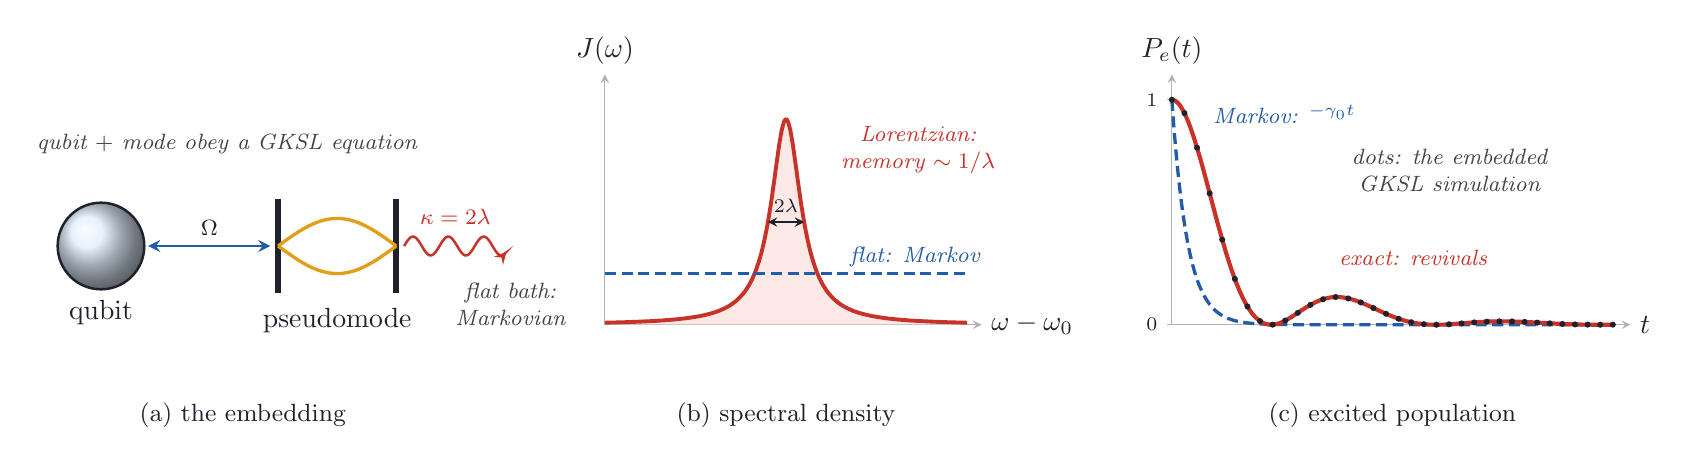
\begin{tikzpicture}[ink/.style={line width=0.9pt, ndInk}, faint/.style={line width=0.4pt, ndInk!35}, dashedink/.style={line width=0.5pt, ndInk!55, dash pattern=on 2.5pt off 2pt}, vec/.style={->, >=stealth, line width=1.2pt}, note/.style={font=\footnotesize\itshape, text=ndInk!85, align=center}, pointer/.style={->, >=stealth, line width=0.4pt, ndInk!60, shorten >=2pt, shorten <=1pt}, dot/.style={circle, fill=ndInk, inner sep=0pt, minimum size=3.4pt}, wash/.style={fill=ndSky, fill opacity=0.55}, every node/.style={text=ndInk}]
\definecolor{ndInk}{rgb}{0.13,0.13,0.18}
\definecolor{ndPaper}{rgb}{0.99,0.96,0.88}
\definecolor{ndSky}{rgb}{0.84,0.91,0.98}
\definecolor{ndRose}{rgb}{0.98,0.86,0.84}
\definecolor{ndBlue}{rgb}{0.13,0.36,0.66}
\definecolor{ndRed}{rgb}{0.78,0.20,0.16}
\definecolor{ndGold}{rgb}{0.88,0.62,0.10}
\definecolor{ndGreen}{rgb}{0.18,0.52,0.30}
\shade[ball color=ndSky!80!white] (0.000,0.000) circle (0.55);
\draw[ink] (0.000,0.000) circle (0.55);
\node at (0.000,-0.850) {qubit};
\draw[line width=2.2pt, ndInk] (2.250,-0.600) -- (2.250,0.600);
\draw[line width=2.2pt, ndInk] (3.750,-0.600) -- (3.750,0.600);
\draw[line width=1.2pt, ndGold] (2.250,0.000) -- (2.275,0.019) -- (2.301,0.037) -- (2.326,0.056) -- (2.352,0.074) -- (2.377,0.092) -- (2.403,0.110) -- (2.428,0.127) -- (2.453,0.145) -- (2.479,0.161) -- (2.504,0.178) -- (2.530,0.193) -- (2.555,0.209) -- (2.581,0.223) -- (2.606,0.237) -- (2.631,0.251) -- (2.657,0.263) -- (2.682,0.275) -- (2.708,0.286) -- (2.733,0.297) -- (2.758,0.306) -- (2.784,0.315) -- (2.809,0.322) -- (2.835,0.329) -- (2.860,0.335) -- (2.886,0.340) -- (2.911,0.344) -- (2.936,0.347) -- (2.962,0.349) -- (2.987,0.350) -- (3.013,0.350) -- (3.038,0.349) -- (3.064,0.347) -- (3.089,0.344) -- (3.114,0.340) -- (3.140,0.335) -- (3.165,0.329) -- (3.191,0.322) -- (3.216,0.315) -- (3.242,0.306) -- (3.267,0.297) -- (3.292,0.286) -- (3.318,0.275) -- (3.343,0.263) -- (3.369,0.251) -- (3.394,0.237) -- (3.419,0.223) -- (3.445,0.209) -- (3.470,0.193) -- (3.496,0.178) -- (3.521,0.161) -- (3.547,0.145) -- (3.572,0.127) -- (3.597,0.110) -- (3.623,0.092) -- (3.648,0.074) -- (3.674,0.056) -- (3.699,0.037) -- (3.725,0.019) -- (3.750,0.000);
\draw[line width=1.2pt, ndGold] (2.250,-0.000) -- (2.275,-0.019) -- (2.301,-0.037) -- (2.326,-0.056) -- (2.352,-0.074) -- (2.377,-0.092) -- (2.403,-0.110) -- (2.428,-0.127) -- (2.453,-0.145) -- (2.479,-0.161) -- (2.504,-0.178) -- (2.530,-0.193) -- (2.555,-0.209) -- (2.581,-0.223) -- (2.606,-0.237) -- (2.631,-0.251) -- (2.657,-0.263) -- (2.682,-0.275) -- (2.708,-0.286) -- (2.733,-0.297) -- (2.758,-0.306) -- (2.784,-0.315) -- (2.809,-0.322) -- (2.835,-0.329) -- (2.860,-0.335) -- (2.886,-0.340) -- (2.911,-0.344) -- (2.936,-0.347) -- (2.962,-0.349) -- (2.987,-0.350) -- (3.013,-0.350) -- (3.038,-0.349) -- (3.064,-0.347) -- (3.089,-0.344) -- (3.114,-0.340) -- (3.140,-0.335) -- (3.165,-0.329) -- (3.191,-0.322) -- (3.216,-0.315) -- (3.242,-0.306) -- (3.267,-0.297) -- (3.292,-0.286) -- (3.318,-0.275) -- (3.343,-0.263) -- (3.369,-0.251) -- (3.394,-0.237) -- (3.419,-0.223) -- (3.445,-0.209) -- (3.470,-0.193) -- (3.496,-0.178) -- (3.521,-0.161) -- (3.547,-0.145) -- (3.572,-0.127) -- (3.597,-0.110) -- (3.623,-0.092) -- (3.648,-0.074) -- (3.674,-0.056) -- (3.699,-0.037) -- (3.725,-0.019) -- (3.750,-0.000);
\node at (3.000,-0.950) {pseudomode};
\draw[<->, >=stealth, line width=0.9pt, ndBlue] (0.600,0.000) -- (2.150,0.000) node[midway, above, font=\footnotesize] {$\Omega$};
\draw[->, >=stealth, line width=0.9pt, ndRed] (3.850,0.000) -- (3.872,0.036) -- (3.894,0.069) -- (3.916,0.096) -- (3.938,0.113) -- (3.960,0.120) -- (3.982,0.115) -- (4.004,0.100) -- (4.026,0.075) -- (4.048,0.043) -- (4.070,0.007) -- (4.092,-0.030) -- (4.114,-0.064) -- (4.136,-0.092) -- (4.158,-0.111) -- (4.181,-0.120) -- (4.203,-0.117) -- (4.225,-0.103) -- (4.247,-0.080) -- (4.269,-0.049) -- (4.291,-0.014) -- (4.313,0.023) -- (4.335,0.058) -- (4.357,0.087) -- (4.379,0.108) -- (4.401,0.119) -- (4.423,0.118) -- (4.445,0.107) -- (4.467,0.085) -- (4.489,0.055) -- (4.511,0.020) -- (4.533,-0.016) -- (4.555,-0.052) -- (4.577,-0.082) -- (4.599,-0.105) -- (4.621,-0.118) -- (4.643,-0.119) -- (4.665,-0.110) -- (4.687,-0.090) -- (4.709,-0.061) -- (4.731,-0.027) -- (4.753,0.010) -- (4.775,0.046) -- (4.797,0.077) -- (4.819,0.101) -- (4.842,0.116) -- (4.864,0.120) -- (4.886,0.112) -- (4.908,0.094) -- (4.930,0.067) -- (4.952,0.034) -- (4.974,-0.003) -- (4.996,-0.039) -- (5.018,-0.072) -- (5.040,-0.098) -- (5.062,-0.114) -- (5.084,-0.120) -- (5.106,-0.114) -- (5.128,-0.098) -- (5.150,-0.073);
\node[font=\footnotesize, text=ndRed, above] at (4.500,0.150) {$\kappa=2\lambda$};
\node[note, anchor=north] at (5.200,-0.350) {flat bath:\\ Markovian};
\node[note, anchor=south] at (1.600,1.050) {qubit $+$ mode obey a GKSL equation};
\node[font=\small] at (1.8,-2.15) {(a) the embedding};
\draw[faint, ->, >=stealth] (6.400,-1.000) -- (11.184,-1.000) node[right, text=ndInk] {$\omega-\omega_0$};
\draw[faint, ->, >=stealth] (6.400,-1.000) -- (6.400,2.180) node[above, text=ndInk] {$J(\omega)$};
\fill[ndRose, fill opacity=0.6] (6.400,-1.000) -- (6.400,-0.974) -- (6.415,-0.974) -- (6.431,-0.973) -- (6.446,-0.973) -- (6.462,-0.973) -- (6.477,-0.972) -- (6.492,-0.972) -- (6.508,-0.972) -- (6.523,-0.971) -- (6.538,-0.971) -- (6.554,-0.970) -- (6.569,-0.970) -- (6.585,-0.970) -- (6.600,-0.969) -- (6.615,-0.969) -- (6.631,-0.968) -- (6.646,-0.968) -- (6.662,-0.967) -- (6.677,-0.967) -- (6.692,-0.966) -- (6.708,-0.966) -- (6.723,-0.965) -- (6.738,-0.965) -- (6.754,-0.964) -- (6.769,-0.963) -- (6.785,-0.963) -- (6.800,-0.962) -- (6.815,-0.962) -- (6.831,-0.961) -- (6.846,-0.960) -- (6.862,-0.960) -- (6.877,-0.959) -- (6.892,-0.958) -- (6.908,-0.958) -- (6.923,-0.957) -- (6.938,-0.956) -- (6.954,-0.956) -- (6.969,-0.955) -- (6.985,-0.954) -- (7.000,-0.953) -- (7.015,-0.952) -- (7.031,-0.951) -- (7.046,-0.951) -- (7.062,-0.950) -- (7.077,-0.949) -- (7.092,-0.948) -- (7.108,-0.947) -- (7.123,-0.946) -- (7.138,-0.945) -- (7.154,-0.944) -- (7.169,-0.942) -- (7.185,-0.941) -- (7.200,-0.940) -- (7.215,-0.939) -- (7.231,-0.938) -- (7.246,-0.936) -- (7.262,-0.935) -- (7.277,-0.934) -- (7.292,-0.932) -- (7.308,-0.931) -- (7.323,-0.929) -- (7.338,-0.928) -- (7.354,-0.926) -- (7.369,-0.924) -- (7.385,-0.923) -- (7.400,-0.921) -- (7.415,-0.919) -- (7.431,-0.917) -- (7.446,-0.915) -- (7.462,-0.913) -- (7.477,-0.911) -- (7.492,-0.909) -- (7.508,-0.906) -- (7.523,-0.904) -- (7.538,-0.902) -- (7.554,-0.899) -- (7.569,-0.896) -- (7.585,-0.894) -- (7.600,-0.891) -- (7.615,-0.888) -- (7.631,-0.885) -- (7.646,-0.881) -- (7.662,-0.878) -- (7.677,-0.874) -- (7.692,-0.871) -- (7.708,-0.867) -- (7.723,-0.863) -- (7.738,-0.859) -- (7.754,-0.854) -- (7.769,-0.850) -- (7.785,-0.845) -- (7.800,-0.840) -- (7.815,-0.835) -- (7.831,-0.829) -- (7.846,-0.824) -- (7.862,-0.817) -- (7.877,-0.811) -- (7.892,-0.804) -- (7.908,-0.797) -- (7.923,-0.790) -- (7.938,-0.782) -- (7.954,-0.774) -- (7.969,-0.765) -- (7.985,-0.756) -- (8.000,-0.746) -- (8.015,-0.735) -- (8.031,-0.724) -- (8.046,-0.713) -- (8.062,-0.700) -- (8.077,-0.687) -- (8.092,-0.673) -- (8.108,-0.658) -- (8.123,-0.642) -- (8.138,-0.625) -- (8.154,-0.607) -- (8.169,-0.588) -- (8.185,-0.567) -- (8.200,-0.544) -- (8.215,-0.520) -- (8.231,-0.495) -- (8.246,-0.467) -- (8.262,-0.437) -- (8.277,-0.405) -- (8.292,-0.370) -- (8.308,-0.333) -- (8.323,-0.292) -- (8.338,-0.248) -- (8.354,-0.201) -- (8.369,-0.150) -- (8.385,-0.094) -- (8.400,-0.034) -- (8.415,0.031) -- (8.431,0.101) -- (8.446,0.176) -- (8.462,0.257) -- (8.477,0.344) -- (8.492,0.437) -- (8.508,0.535) -- (8.523,0.639) -- (8.538,0.747) -- (8.554,0.858) -- (8.569,0.971) -- (8.585,1.084) -- (8.600,1.194) -- (8.615,1.298) -- (8.631,1.392) -- (8.646,1.473) -- (8.662,1.538) -- (8.677,1.583) -- (8.692,1.606) -- (8.708,1.606) -- (8.723,1.583) -- (8.738,1.538) -- (8.754,1.473) -- (8.769,1.392) -- (8.785,1.298) -- (8.800,1.194) -- (8.815,1.084) -- (8.831,0.971) -- (8.846,0.858) -- (8.862,0.747) -- (8.877,0.639) -- (8.892,0.535) -- (8.908,0.437) -- (8.923,0.344) -- (8.938,0.257) -- (8.954,0.176) -- (8.969,0.101) -- (8.985,0.031) -- (9.000,-0.034) -- (9.015,-0.094) -- (9.031,-0.150) -- (9.046,-0.201) -- (9.062,-0.248) -- (9.077,-0.292) -- (9.092,-0.333) -- (9.108,-0.370) -- (9.123,-0.405) -- (9.138,-0.437) -- (9.154,-0.467) -- (9.169,-0.495) -- (9.185,-0.520) -- (9.200,-0.544) -- (9.215,-0.567) -- (9.231,-0.588) -- (9.246,-0.607) -- (9.262,-0.625) -- (9.277,-0.642) -- (9.292,-0.658) -- (9.308,-0.673) -- (9.323,-0.687) -- (9.338,-0.700) -- (9.354,-0.713) -- (9.369,-0.724) -- (9.385,-0.735) -- (9.400,-0.746) -- (9.415,-0.756) -- (9.431,-0.765) -- (9.446,-0.774) -- (9.462,-0.782) -- (9.477,-0.790) -- (9.492,-0.797) -- (9.508,-0.804) -- (9.523,-0.811) -- (9.538,-0.817) -- (9.554,-0.824) -- (9.569,-0.829) -- (9.585,-0.835) -- (9.600,-0.840) -- (9.615,-0.845) -- (9.631,-0.850) -- (9.646,-0.854) -- (9.662,-0.859) -- (9.677,-0.863) -- (9.692,-0.867) -- (9.708,-0.871) -- (9.723,-0.874) -- (9.738,-0.878) -- (9.754,-0.881) -- (9.769,-0.885) -- (9.785,-0.888) -- (9.800,-0.891) -- (9.815,-0.894) -- (9.831,-0.896) -- (9.846,-0.899) -- (9.862,-0.902) -- (9.877,-0.904) -- (9.892,-0.906) -- (9.908,-0.909) -- (9.923,-0.911) -- (9.938,-0.913) -- (9.954,-0.915) -- (9.969,-0.917) -- (9.985,-0.919) -- (10.000,-0.921) -- (10.015,-0.923) -- (10.031,-0.924) -- (10.046,-0.926) -- (10.062,-0.928) -- (10.077,-0.929) -- (10.092,-0.931) -- (10.108,-0.932) -- (10.123,-0.934) -- (10.138,-0.935) -- (10.154,-0.936) -- (10.169,-0.938) -- (10.185,-0.939) -- (10.200,-0.940) -- (10.215,-0.941) -- (10.231,-0.942) -- (10.246,-0.944) -- (10.262,-0.945) -- (10.277,-0.946) -- (10.292,-0.947) -- (10.308,-0.948) -- (10.323,-0.949) -- (10.338,-0.950) -- (10.354,-0.951) -- (10.369,-0.951) -- (10.385,-0.952) -- (10.400,-0.953) -- (10.415,-0.954) -- (10.431,-0.955) -- (10.446,-0.956) -- (10.462,-0.956) -- (10.477,-0.957) -- (10.492,-0.958) -- (10.508,-0.958) -- (10.523,-0.959) -- (10.538,-0.960) -- (10.554,-0.960) -- (10.569,-0.961) -- (10.585,-0.962) -- (10.600,-0.962) -- (10.615,-0.963) -- (10.631,-0.963) -- (10.646,-0.964) -- (10.662,-0.965) -- (10.677,-0.965) -- (10.692,-0.966) -- (10.708,-0.966) -- (10.723,-0.967) -- (10.738,-0.967) -- (10.754,-0.968) -- (10.769,-0.968) -- (10.785,-0.969) -- (10.800,-0.969) -- (10.815,-0.970) -- (10.831,-0.970) -- (10.846,-0.970) -- (10.862,-0.971) -- (10.877,-0.971) -- (10.892,-0.972) -- (10.908,-0.972) -- (10.923,-0.972) -- (10.938,-0.973) -- (10.954,-0.973) -- (10.969,-0.973) -- (10.985,-0.974) -- (11.000,-0.974) -- (11.000,-1.000) -- cycle;
\draw[line width=1.4pt, ndRed] (6.400,-0.974) -- (6.415,-0.974) -- (6.431,-0.973) -- (6.446,-0.973) -- (6.462,-0.973) -- (6.477,-0.972) -- (6.492,-0.972) -- (6.508,-0.972) -- (6.523,-0.971) -- (6.538,-0.971) -- (6.554,-0.970) -- (6.569,-0.970) -- (6.585,-0.970) -- (6.600,-0.969) -- (6.615,-0.969) -- (6.631,-0.968) -- (6.646,-0.968) -- (6.662,-0.967) -- (6.677,-0.967) -- (6.692,-0.966) -- (6.708,-0.966) -- (6.723,-0.965) -- (6.738,-0.965) -- (6.754,-0.964) -- (6.769,-0.963) -- (6.785,-0.963) -- (6.800,-0.962) -- (6.815,-0.962) -- (6.831,-0.961) -- (6.846,-0.960) -- (6.862,-0.960) -- (6.877,-0.959) -- (6.892,-0.958) -- (6.908,-0.958) -- (6.923,-0.957) -- (6.938,-0.956) -- (6.954,-0.956) -- (6.969,-0.955) -- (6.985,-0.954) -- (7.000,-0.953) -- (7.015,-0.952) -- (7.031,-0.951) -- (7.046,-0.951) -- (7.062,-0.950) -- (7.077,-0.949) -- (7.092,-0.948) -- (7.108,-0.947) -- (7.123,-0.946) -- (7.138,-0.945) -- (7.154,-0.944) -- (7.169,-0.942) -- (7.185,-0.941) -- (7.200,-0.940) -- (7.215,-0.939) -- (7.231,-0.938) -- (7.246,-0.936) -- (7.262,-0.935) -- (7.277,-0.934) -- (7.292,-0.932) -- (7.308,-0.931) -- (7.323,-0.929) -- (7.338,-0.928) -- (7.354,-0.926) -- (7.369,-0.924) -- (7.385,-0.923) -- (7.400,-0.921) -- (7.415,-0.919) -- (7.431,-0.917) -- (7.446,-0.915) -- (7.462,-0.913) -- (7.477,-0.911) -- (7.492,-0.909) -- (7.508,-0.906) -- (7.523,-0.904) -- (7.538,-0.902) -- (7.554,-0.899) -- (7.569,-0.896) -- (7.585,-0.894) -- (7.600,-0.891) -- (7.615,-0.888) -- (7.631,-0.885) -- (7.646,-0.881) -- (7.662,-0.878) -- (7.677,-0.874) -- (7.692,-0.871) -- (7.708,-0.867) -- (7.723,-0.863) -- (7.738,-0.859) -- (7.754,-0.854) -- (7.769,-0.850) -- (7.785,-0.845) -- (7.800,-0.840) -- (7.815,-0.835) -- (7.831,-0.829) -- (7.846,-0.824) -- (7.862,-0.817) -- (7.877,-0.811) -- (7.892,-0.804) -- (7.908,-0.797) -- (7.923,-0.790) -- (7.938,-0.782) -- (7.954,-0.774) -- (7.969,-0.765) -- (7.985,-0.756) -- (8.000,-0.746) -- (8.015,-0.735) -- (8.031,-0.724) -- (8.046,-0.713) -- (8.062,-0.700) -- (8.077,-0.687) -- (8.092,-0.673) -- (8.108,-0.658) -- (8.123,-0.642) -- (8.138,-0.625) -- (8.154,-0.607) -- (8.169,-0.588) -- (8.185,-0.567) -- (8.200,-0.544) -- (8.215,-0.520) -- (8.231,-0.495) -- (8.246,-0.467) -- (8.262,-0.437) -- (8.277,-0.405) -- (8.292,-0.370) -- (8.308,-0.333) -- (8.323,-0.292) -- (8.338,-0.248) -- (8.354,-0.201) -- (8.369,-0.150) -- (8.385,-0.094) -- (8.400,-0.034) -- (8.415,0.031) -- (8.431,0.101) -- (8.446,0.176) -- (8.462,0.257) -- (8.477,0.344) -- (8.492,0.437) -- (8.508,0.535) -- (8.523,0.639) -- (8.538,0.747) -- (8.554,0.858) -- (8.569,0.971) -- (8.585,1.084) -- (8.600,1.194) -- (8.615,1.298) -- (8.631,1.392) -- (8.646,1.473) -- (8.662,1.538) -- (8.677,1.583) -- (8.692,1.606) -- (8.708,1.606) -- (8.723,1.583) -- (8.738,1.538) -- (8.754,1.473) -- (8.769,1.392) -- (8.785,1.298) -- (8.800,1.194) -- (8.815,1.084) -- (8.831,0.971) -- (8.846,0.858) -- (8.862,0.747) -- (8.877,0.639) -- (8.892,0.535) -- (8.908,0.437) -- (8.923,0.344) -- (8.938,0.257) -- (8.954,0.176) -- (8.969,0.101) -- (8.985,0.031) -- (9.000,-0.034) -- (9.015,-0.094) -- (9.031,-0.150) -- (9.046,-0.201) -- (9.062,-0.248) -- (9.077,-0.292) -- (9.092,-0.333) -- (9.108,-0.370) -- (9.123,-0.405) -- (9.138,-0.437) -- (9.154,-0.467) -- (9.169,-0.495) -- (9.185,-0.520) -- (9.200,-0.544) -- (9.215,-0.567) -- (9.231,-0.588) -- (9.246,-0.607) -- (9.262,-0.625) -- (9.277,-0.642) -- (9.292,-0.658) -- (9.308,-0.673) -- (9.323,-0.687) -- (9.338,-0.700) -- (9.354,-0.713) -- (9.369,-0.724) -- (9.385,-0.735) -- (9.400,-0.746) -- (9.415,-0.756) -- (9.431,-0.765) -- (9.446,-0.774) -- (9.462,-0.782) -- (9.477,-0.790) -- (9.492,-0.797) -- (9.508,-0.804) -- (9.523,-0.811) -- (9.538,-0.817) -- (9.554,-0.824) -- (9.569,-0.829) -- (9.585,-0.835) -- (9.600,-0.840) -- (9.615,-0.845) -- (9.631,-0.850) -- (9.646,-0.854) -- (9.662,-0.859) -- (9.677,-0.863) -- (9.692,-0.867) -- (9.708,-0.871) -- (9.723,-0.874) -- (9.738,-0.878) -- (9.754,-0.881) -- (9.769,-0.885) -- (9.785,-0.888) -- (9.800,-0.891) -- (9.815,-0.894) -- (9.831,-0.896) -- (9.846,-0.899) -- (9.862,-0.902) -- (9.877,-0.904) -- (9.892,-0.906) -- (9.908,-0.909) -- (9.923,-0.911) -- (9.938,-0.913) -- (9.954,-0.915) -- (9.969,-0.917) -- (9.985,-0.919) -- (10.000,-0.921) -- (10.015,-0.923) -- (10.031,-0.924) -- (10.046,-0.926) -- (10.062,-0.928) -- (10.077,-0.929) -- (10.092,-0.931) -- (10.108,-0.932) -- (10.123,-0.934) -- (10.138,-0.935) -- (10.154,-0.936) -- (10.169,-0.938) -- (10.185,-0.939) -- (10.200,-0.940) -- (10.215,-0.941) -- (10.231,-0.942) -- (10.246,-0.944) -- (10.262,-0.945) -- (10.277,-0.946) -- (10.292,-0.947) -- (10.308,-0.948) -- (10.323,-0.949) -- (10.338,-0.950) -- (10.354,-0.951) -- (10.369,-0.951) -- (10.385,-0.952) -- (10.400,-0.953) -- (10.415,-0.954) -- (10.431,-0.955) -- (10.446,-0.956) -- (10.462,-0.956) -- (10.477,-0.957) -- (10.492,-0.958) -- (10.508,-0.958) -- (10.523,-0.959) -- (10.538,-0.960) -- (10.554,-0.960) -- (10.569,-0.961) -- (10.585,-0.962) -- (10.600,-0.962) -- (10.615,-0.963) -- (10.631,-0.963) -- (10.646,-0.964) -- (10.662,-0.965) -- (10.677,-0.965) -- (10.692,-0.966) -- (10.708,-0.966) -- (10.723,-0.967) -- (10.738,-0.967) -- (10.754,-0.968) -- (10.769,-0.968) -- (10.785,-0.969) -- (10.800,-0.969) -- (10.815,-0.970) -- (10.831,-0.970) -- (10.846,-0.970) -- (10.862,-0.971) -- (10.877,-0.971) -- (10.892,-0.972) -- (10.908,-0.972) -- (10.923,-0.972) -- (10.938,-0.973) -- (10.954,-0.973) -- (10.969,-0.973) -- (10.985,-0.974) -- (11.000,-0.974);
\draw[line width=1.2pt, ndBlue, dash pattern=on 4pt off 2pt] (6.400,-0.348) -- (11.000,-0.348);
\draw[<->, >=stealth, ndInk, line width=0.5pt] (8.470,0.304) -- (8.930,0.304) node[midway, above, font=\scriptsize] {$2\lambda$};
\node[note, anchor=west, text=ndBlue] at (9.390,-0.139) {flat: Markov};
\node[note, anchor=west, text=ndRed] at (9.275,1.217) {Lorentzian:\\ memory $\sim1/\lambda$};
\node[font=\small] at (8.700,-2.150) {(b) spectral density};
\draw[faint, ->, >=stealth] (13.600,-1.000) -- (19.424,-1.000) node[right, text=ndInk] {$t$};
\draw[faint, ->, >=stealth] (13.600,-1.000) -- (13.600,2.180) node[above, text=ndInk] {$P_e(t)$};
\draw[faint] (13.660,-1.000) -- (13.540,-1.000) node[left, font=\scriptsize, text=ndInk] {$0$};
\draw[faint] (13.660,1.857) -- (13.540,1.857) node[left, font=\scriptsize, text=ndInk] {$1$};
\draw[line width=1.2pt, ndBlue, dash pattern=on 4pt off 2pt] (13.600,1.857) -- (13.608,1.745) -- (13.616,1.637) -- (13.624,1.534) -- (13.632,1.434) -- (13.640,1.339) -- (13.648,1.247) -- (13.656,1.159) -- (13.664,1.074) -- (13.672,0.992) -- (13.680,0.914) -- (13.688,0.839) -- (13.696,0.767) -- (13.704,0.697) -- (13.712,0.631) -- (13.720,0.567) -- (13.728,0.505) -- (13.736,0.446) -- (13.744,0.389) -- (13.752,0.335) -- (13.760,0.282) -- (13.768,0.232) -- (13.776,0.184) -- (13.784,0.137) -- (13.792,0.092) -- (13.800,0.050) -- (13.808,0.008) -- (13.816,-0.031) -- (13.824,-0.069) -- (13.832,-0.106) -- (13.840,-0.141) -- (13.848,-0.175) -- (13.856,-0.207) -- (13.864,-0.238) -- (13.872,-0.268) -- (13.880,-0.297) -- (13.888,-0.324) -- (13.896,-0.351) -- (13.904,-0.376) -- (13.912,-0.401) -- (13.920,-0.424) -- (13.928,-0.447) -- (13.936,-0.469) -- (13.944,-0.490) -- (13.953,-0.510) -- (13.961,-0.529) -- (13.969,-0.547) -- (13.977,-0.565) -- (13.985,-0.582) -- (13.993,-0.599) -- (14.001,-0.614) -- (14.009,-0.630) -- (14.017,-0.644) -- (14.025,-0.658) -- (14.033,-0.672) -- (14.041,-0.684) -- (14.049,-0.697) -- (14.057,-0.709) -- (14.065,-0.720) -- (14.073,-0.731) -- (14.081,-0.742) -- (14.089,-0.752) -- (14.097,-0.762) -- (14.105,-0.771) -- (14.113,-0.780) -- (14.121,-0.789) -- (14.129,-0.797) -- (14.137,-0.805) -- (14.145,-0.813) -- (14.153,-0.820) -- (14.161,-0.827) -- (14.169,-0.834) -- (14.177,-0.840) -- (14.185,-0.847) -- (14.193,-0.853) -- (14.201,-0.858) -- (14.209,-0.864) -- (14.217,-0.869) -- (14.225,-0.874) -- (14.233,-0.879) -- (14.241,-0.884) -- (14.249,-0.889) -- (14.257,-0.893) -- (14.265,-0.897) -- (14.273,-0.901) -- (14.281,-0.905) -- (14.289,-0.909) -- (14.297,-0.912) -- (14.305,-0.916) -- (14.313,-0.919) -- (14.321,-0.922) -- (14.329,-0.925) -- (14.337,-0.928) -- (14.345,-0.931) -- (14.353,-0.934) -- (14.361,-0.936) -- (14.369,-0.939) -- (14.377,-0.941) -- (14.385,-0.944) -- (14.393,-0.946) -- (14.401,-0.948) -- (14.409,-0.950) -- (14.417,-0.952) -- (14.425,-0.954) -- (14.433,-0.956) -- (14.441,-0.957) -- (14.449,-0.959) -- (14.457,-0.961) -- (14.465,-0.962) -- (14.473,-0.964) -- (14.481,-0.965) -- (14.489,-0.967) -- (14.497,-0.968) -- (14.505,-0.969) -- (14.513,-0.970) -- (14.521,-0.971) -- (14.529,-0.973) -- (14.537,-0.974) -- (14.545,-0.975) -- (14.553,-0.976) -- (14.561,-0.977) -- (14.569,-0.978) -- (14.577,-0.978) -- (14.585,-0.979) -- (14.593,-0.980) -- (14.601,-0.981) -- (14.609,-0.982) -- (14.617,-0.982) -- (14.625,-0.983) -- (14.633,-0.984) -- (14.641,-0.984) -- (14.649,-0.985) -- (14.658,-0.986) -- (14.666,-0.986) -- (14.674,-0.987) -- (14.682,-0.987) -- (14.690,-0.988) -- (14.698,-0.988) -- (14.706,-0.989) -- (14.714,-0.989) -- (14.722,-0.990) -- (14.730,-0.990) -- (14.738,-0.990) -- (14.746,-0.991) -- (14.754,-0.991) -- (14.762,-0.991) -- (14.770,-0.992) -- (14.778,-0.992) -- (14.786,-0.992) -- (14.794,-0.993) -- (14.802,-0.993) -- (14.810,-0.993) -- (14.818,-0.994) -- (14.826,-0.994) -- (14.834,-0.994) -- (14.842,-0.994) -- (14.850,-0.994) -- (14.858,-0.995) -- (14.866,-0.995) -- (14.874,-0.995) -- (14.882,-0.995) -- (14.890,-0.995) -- (14.898,-0.996) -- (14.906,-0.996) -- (14.914,-0.996) -- (14.922,-0.996) -- (14.930,-0.996) -- (14.938,-0.996) -- (14.946,-0.997) -- (14.954,-0.997) -- (14.962,-0.997) -- (14.970,-0.997) -- (14.978,-0.997) -- (14.986,-0.997) -- (14.994,-0.997) -- (15.002,-0.997) -- (15.010,-0.998) -- (15.018,-0.998) -- (15.026,-0.998) -- (15.034,-0.998) -- (15.042,-0.998) -- (15.050,-0.998) -- (15.058,-0.998) -- (15.066,-0.998) -- (15.074,-0.998) -- (15.082,-0.998) -- (15.090,-0.998) -- (15.098,-0.998) -- (15.106,-0.998) -- (15.114,-0.999) -- (15.122,-0.999) -- (15.130,-0.999) -- (15.138,-0.999) -- (15.146,-0.999) -- (15.154,-0.999) -- (15.162,-0.999) -- (15.170,-0.999) -- (15.178,-0.999) -- (15.186,-0.999) -- (15.194,-0.999) -- (15.202,-0.999) -- (15.210,-0.999) -- (15.218,-0.999) -- (15.226,-0.999) -- (15.234,-0.999) -- (15.242,-0.999) -- (15.250,-0.999) -- (15.258,-0.999) -- (15.266,-0.999) -- (15.274,-0.999) -- (15.282,-0.999) -- (15.290,-0.999) -- (15.298,-0.999) -- (15.306,-0.999) -- (15.314,-0.999) -- (15.322,-0.999) -- (15.330,-1.000) -- (15.338,-1.000) -- (15.346,-1.000) -- (15.355,-1.000) -- (15.363,-1.000) -- (15.371,-1.000) -- (15.379,-1.000) -- (15.387,-1.000) -- (15.395,-1.000) -- (15.403,-1.000) -- (15.411,-1.000) -- (15.419,-1.000) -- (15.427,-1.000) -- (15.435,-1.000) -- (15.443,-1.000) -- (15.451,-1.000) -- (15.459,-1.000) -- (15.467,-1.000) -- (15.475,-1.000) -- (15.483,-1.000) -- (15.491,-1.000) -- (15.499,-1.000) -- (15.507,-1.000) -- (15.515,-1.000) -- (15.523,-1.000) -- (15.531,-1.000) -- (15.539,-1.000) -- (15.547,-1.000) -- (15.555,-1.000) -- (15.563,-1.000) -- (15.571,-1.000) -- (15.579,-1.000) -- (15.587,-1.000) -- (15.595,-1.000) -- (15.603,-1.000) -- (15.611,-1.000) -- (15.619,-1.000) -- (15.627,-1.000) -- (15.635,-1.000) -- (15.643,-1.000) -- (15.651,-1.000) -- (15.659,-1.000) -- (15.667,-1.000) -- (15.675,-1.000) -- (15.683,-1.000) -- (15.691,-1.000) -- (15.699,-1.000) -- (15.707,-1.000) -- (15.715,-1.000) -- (15.723,-1.000) -- (15.731,-1.000) -- (15.739,-1.000) -- (15.747,-1.000) -- (15.755,-1.000) -- (15.763,-1.000) -- (15.771,-1.000) -- (15.779,-1.000) -- (15.787,-1.000) -- (15.795,-1.000) -- (15.803,-1.000) -- (15.811,-1.000) -- (15.819,-1.000) -- (15.827,-1.000) -- (15.835,-1.000) -- (15.843,-1.000) -- (15.851,-1.000) -- (15.859,-1.000) -- (15.867,-1.000) -- (15.875,-1.000) -- (15.883,-1.000) -- (15.891,-1.000) -- (15.899,-1.000) -- (15.907,-1.000) -- (15.915,-1.000) -- (15.923,-1.000) -- (15.931,-1.000) -- (15.939,-1.000) -- (15.947,-1.000) -- (15.955,-1.000) -- (15.963,-1.000) -- (15.971,-1.000) -- (15.979,-1.000) -- (15.987,-1.000) -- (15.995,-1.000) -- (16.003,-1.000) -- (16.011,-1.000) -- (16.019,-1.000) -- (16.027,-1.000) -- (16.035,-1.000) -- (16.043,-1.000) -- (16.052,-1.000) -- (16.060,-1.000) -- (16.068,-1.000) -- (16.076,-1.000) -- (16.084,-1.000) -- (16.092,-1.000) -- (16.100,-1.000) -- (16.108,-1.000) -- (16.116,-1.000) -- (16.124,-1.000) -- (16.132,-1.000) -- (16.140,-1.000) -- (16.148,-1.000) -- (16.156,-1.000) -- (16.164,-1.000) -- (16.172,-1.000) -- (16.180,-1.000) -- (16.188,-1.000) -- (16.196,-1.000) -- (16.204,-1.000) -- (16.212,-1.000) -- (16.220,-1.000) -- (16.228,-1.000) -- (16.236,-1.000) -- (16.244,-1.000) -- (16.252,-1.000) -- (16.260,-1.000) -- (16.268,-1.000) -- (16.276,-1.000) -- (16.284,-1.000) -- (16.292,-1.000) -- (16.300,-1.000) -- (16.308,-1.000) -- (16.316,-1.000) -- (16.324,-1.000) -- (16.332,-1.000) -- (16.340,-1.000) -- (16.348,-1.000) -- (16.356,-1.000) -- (16.364,-1.000) -- (16.372,-1.000) -- (16.380,-1.000) -- (16.388,-1.000) -- (16.396,-1.000) -- (16.404,-1.000) -- (16.412,-1.000) -- (16.420,-1.000) -- (16.428,-1.000) -- (16.436,-1.000) -- (16.444,-1.000) -- (16.452,-1.000) -- (16.460,-1.000) -- (16.468,-1.000) -- (16.476,-1.000) -- (16.484,-1.000) -- (16.492,-1.000) -- (16.500,-1.000) -- (16.508,-1.000) -- (16.516,-1.000) -- (16.524,-1.000) -- (16.532,-1.000) -- (16.540,-1.000) -- (16.548,-1.000) -- (16.556,-1.000) -- (16.564,-1.000) -- (16.572,-1.000) -- (16.580,-1.000) -- (16.588,-1.000) -- (16.596,-1.000) -- (16.604,-1.000) -- (16.612,-1.000) -- (16.620,-1.000) -- (16.628,-1.000) -- (16.636,-1.000) -- (16.644,-1.000) -- (16.652,-1.000) -- (16.660,-1.000) -- (16.668,-1.000) -- (16.676,-1.000) -- (16.684,-1.000) -- (16.692,-1.000) -- (16.700,-1.000) -- (16.708,-1.000) -- (16.716,-1.000) -- (16.724,-1.000) -- (16.732,-1.000) -- (16.740,-1.000) -- (16.748,-1.000) -- (16.757,-1.000) -- (16.765,-1.000) -- (16.773,-1.000) -- (16.781,-1.000) -- (16.789,-1.000) -- (16.797,-1.000) -- (16.805,-1.000) -- (16.813,-1.000) -- (16.821,-1.000) -- (16.829,-1.000) -- (16.837,-1.000) -- (16.845,-1.000) -- (16.853,-1.000) -- (16.861,-1.000) -- (16.869,-1.000) -- (16.877,-1.000) -- (16.885,-1.000) -- (16.893,-1.000) -- (16.901,-1.000) -- (16.909,-1.000) -- (16.917,-1.000) -- (16.925,-1.000) -- (16.933,-1.000) -- (16.941,-1.000) -- (16.949,-1.000) -- (16.957,-1.000) -- (16.965,-1.000) -- (16.973,-1.000) -- (16.981,-1.000) -- (16.989,-1.000) -- (16.997,-1.000) -- (17.005,-1.000) -- (17.013,-1.000) -- (17.021,-1.000) -- (17.029,-1.000) -- (17.037,-1.000) -- (17.045,-1.000) -- (17.053,-1.000) -- (17.061,-1.000) -- (17.069,-1.000) -- (17.077,-1.000) -- (17.085,-1.000) -- (17.093,-1.000) -- (17.101,-1.000) -- (17.109,-1.000) -- (17.117,-1.000) -- (17.125,-1.000) -- (17.133,-1.000) -- (17.141,-1.000) -- (17.149,-1.000) -- (17.157,-1.000) -- (17.165,-1.000) -- (17.173,-1.000) -- (17.181,-1.000) -- (17.189,-1.000) -- (17.197,-1.000) -- (17.205,-1.000) -- (17.213,-1.000) -- (17.221,-1.000) -- (17.229,-1.000) -- (17.237,-1.000) -- (17.245,-1.000) -- (17.253,-1.000) -- (17.261,-1.000) -- (17.269,-1.000) -- (17.277,-1.000) -- (17.285,-1.000) -- (17.293,-1.000) -- (17.301,-1.000) -- (17.309,-1.000) -- (17.317,-1.000) -- (17.325,-1.000) -- (17.333,-1.000) -- (17.341,-1.000) -- (17.349,-1.000) -- (17.357,-1.000) -- (17.365,-1.000) -- (17.373,-1.000) -- (17.381,-1.000) -- (17.389,-1.000) -- (17.397,-1.000) -- (17.405,-1.000) -- (17.413,-1.000) -- (17.421,-1.000) -- (17.429,-1.000) -- (17.437,-1.000) -- (17.445,-1.000) -- (17.454,-1.000) -- (17.462,-1.000) -- (17.470,-1.000) -- (17.478,-1.000) -- (17.486,-1.000) -- (17.494,-1.000) -- (17.502,-1.000) -- (17.510,-1.000) -- (17.518,-1.000) -- (17.526,-1.000) -- (17.534,-1.000) -- (17.542,-1.000) -- (17.550,-1.000) -- (17.558,-1.000) -- (17.566,-1.000) -- (17.574,-1.000) -- (17.582,-1.000) -- (17.590,-1.000) -- (17.598,-1.000) -- (17.606,-1.000) -- (17.614,-1.000) -- (17.622,-1.000) -- (17.630,-1.000) -- (17.638,-1.000) -- (17.646,-1.000) -- (17.654,-1.000) -- (17.662,-1.000) -- (17.670,-1.000) -- (17.678,-1.000) -- (17.686,-1.000) -- (17.694,-1.000) -- (17.702,-1.000) -- (17.710,-1.000) -- (17.718,-1.000) -- (17.726,-1.000) -- (17.734,-1.000) -- (17.742,-1.000) -- (17.750,-1.000) -- (17.758,-1.000) -- (17.766,-1.000) -- (17.774,-1.000) -- (17.782,-1.000) -- (17.790,-1.000) -- (17.798,-1.000) -- (17.806,-1.000) -- (17.814,-1.000) -- (17.822,-1.000) -- (17.830,-1.000) -- (17.838,-1.000) -- (17.846,-1.000) -- (17.854,-1.000) -- (17.862,-1.000) -- (17.870,-1.000) -- (17.878,-1.000) -- (17.886,-1.000) -- (17.894,-1.000) -- (17.902,-1.000) -- (17.910,-1.000) -- (17.918,-1.000) -- (17.926,-1.000) -- (17.934,-1.000) -- (17.942,-1.000) -- (17.950,-1.000) -- (17.958,-1.000) -- (17.966,-1.000) -- (17.974,-1.000) -- (17.982,-1.000) -- (17.990,-1.000) -- (17.998,-1.000) -- (18.006,-1.000) -- (18.014,-1.000) -- (18.022,-1.000) -- (18.030,-1.000) -- (18.038,-1.000) -- (18.046,-1.000) -- (18.054,-1.000) -- (18.062,-1.000) -- (18.070,-1.000) -- (18.078,-1.000) -- (18.086,-1.000) -- (18.094,-1.000) -- (18.102,-1.000) -- (18.110,-1.000) -- (18.118,-1.000) -- (18.126,-1.000) -- (18.134,-1.000) -- (18.142,-1.000) -- (18.151,-1.000) -- (18.159,-1.000) -- (18.167,-1.000) -- (18.175,-1.000) -- (18.183,-1.000) -- (18.191,-1.000) -- (18.199,-1.000) -- (18.207,-1.000) -- (18.215,-1.000) -- (18.223,-1.000) -- (18.231,-1.000) -- (18.239,-1.000) -- (18.247,-1.000) -- (18.255,-1.000) -- (18.263,-1.000) -- (18.271,-1.000) -- (18.279,-1.000) -- (18.287,-1.000) -- (18.295,-1.000) -- (18.303,-1.000) -- (18.311,-1.000) -- (18.319,-1.000) -- (18.327,-1.000) -- (18.335,-1.000) -- (18.343,-1.000) -- (18.351,-1.000) -- (18.359,-1.000) -- (18.367,-1.000) -- (18.375,-1.000) -- (18.383,-1.000) -- (18.391,-1.000) -- (18.399,-1.000) -- (18.407,-1.000) -- (18.415,-1.000) -- (18.423,-1.000) -- (18.431,-1.000) -- (18.439,-1.000) -- (18.447,-1.000) -- (18.455,-1.000) -- (18.463,-1.000) -- (18.471,-1.000) -- (18.479,-1.000) -- (18.487,-1.000) -- (18.495,-1.000) -- (18.503,-1.000) -- (18.511,-1.000) -- (18.519,-1.000) -- (18.527,-1.000) -- (18.535,-1.000) -- (18.543,-1.000) -- (18.551,-1.000) -- (18.559,-1.000) -- (18.567,-1.000) -- (18.575,-1.000) -- (18.583,-1.000) -- (18.591,-1.000) -- (18.599,-1.000) -- (18.607,-1.000) -- (18.615,-1.000) -- (18.623,-1.000) -- (18.631,-1.000) -- (18.639,-1.000) -- (18.647,-1.000) -- (18.655,-1.000) -- (18.663,-1.000) -- (18.671,-1.000) -- (18.679,-1.000) -- (18.687,-1.000) -- (18.695,-1.000) -- (18.703,-1.000) -- (18.711,-1.000) -- (18.719,-1.000) -- (18.727,-1.000) -- (18.735,-1.000) -- (18.743,-1.000) -- (18.751,-1.000) -- (18.759,-1.000) -- (18.767,-1.000) -- (18.775,-1.000) -- (18.783,-1.000) -- (18.791,-1.000) -- (18.799,-1.000) -- (18.807,-1.000) -- (18.815,-1.000) -- (18.823,-1.000) -- (18.831,-1.000) -- (18.839,-1.000) -- (18.847,-1.000) -- (18.856,-1.000) -- (18.864,-1.000) -- (18.872,-1.000) -- (18.880,-1.000) -- (18.888,-1.000) -- (18.896,-1.000) -- (18.904,-1.000) -- (18.912,-1.000) -- (18.920,-1.000) -- (18.928,-1.000) -- (18.936,-1.000) -- (18.944,-1.000) -- (18.952,-1.000) -- (18.960,-1.000) -- (18.968,-1.000) -- (18.976,-1.000) -- (18.984,-1.000) -- (18.992,-1.000) -- (19.000,-1.000) -- (19.008,-1.000) -- (19.016,-1.000) -- (19.024,-1.000) -- (19.032,-1.000) -- (19.040,-1.000) -- (19.048,-1.000) -- (19.056,-1.000) -- (19.064,-1.000) -- (19.072,-1.000) -- (19.080,-1.000) -- (19.088,-1.000) -- (19.096,-1.000) -- (19.104,-1.000) -- (19.112,-1.000) -- (19.120,-1.000) -- (19.128,-1.000) -- (19.136,-1.000) -- (19.144,-1.000) -- (19.152,-1.000) -- (19.160,-1.000) -- (19.168,-1.000) -- (19.176,-1.000) -- (19.184,-1.000) -- (19.192,-1.000) -- (19.200,-1.000);
\draw[line width=1.5pt, ndRed] (13.600,1.857) -- (13.608,1.857) -- (13.616,1.855) -- (13.624,1.853) -- (13.632,1.850) -- (13.640,1.846) -- (13.648,1.841) -- (13.656,1.835) -- (13.664,1.829) -- (13.672,1.821) -- (13.680,1.813) -- (13.688,1.804) -- (13.696,1.794) -- (13.704,1.783) -- (13.712,1.771) -- (13.720,1.759) -- (13.728,1.746) -- (13.736,1.732) -- (13.744,1.718) -- (13.752,1.703) -- (13.760,1.687) -- (13.768,1.670) -- (13.776,1.653) -- (13.784,1.635) -- (13.792,1.616) -- (13.800,1.597) -- (13.808,1.577) -- (13.816,1.557) -- (13.824,1.536) -- (13.832,1.515) -- (13.840,1.493) -- (13.848,1.470) -- (13.856,1.447) -- (13.864,1.423) -- (13.872,1.399) -- (13.880,1.375) -- (13.888,1.350) -- (13.896,1.325) -- (13.904,1.299) -- (13.912,1.273) -- (13.920,1.246) -- (13.928,1.220) -- (13.936,1.192) -- (13.944,1.165) -- (13.953,1.137) -- (13.961,1.109) -- (13.969,1.081) -- (13.977,1.052) -- (13.985,1.024) -- (13.993,0.995) -- (14.001,0.965) -- (14.009,0.936) -- (14.017,0.906) -- (14.025,0.877) -- (14.033,0.847) -- (14.041,0.817) -- (14.049,0.787) -- (14.057,0.757) -- (14.065,0.727) -- (14.073,0.697) -- (14.081,0.666) -- (14.089,0.636) -- (14.097,0.606) -- (14.105,0.576) -- (14.113,0.545) -- (14.121,0.515) -- (14.129,0.485) -- (14.137,0.455) -- (14.145,0.425) -- (14.153,0.395) -- (14.161,0.365) -- (14.169,0.336) -- (14.177,0.306) -- (14.185,0.277) -- (14.193,0.248) -- (14.201,0.219) -- (14.209,0.190) -- (14.217,0.161) -- (14.225,0.133) -- (14.233,0.105) -- (14.241,0.077) -- (14.249,0.049) -- (14.257,0.021) -- (14.265,-0.006) -- (14.273,-0.033) -- (14.281,-0.060) -- (14.289,-0.086) -- (14.297,-0.112) -- (14.305,-0.138) -- (14.313,-0.163) -- (14.321,-0.189) -- (14.329,-0.214) -- (14.337,-0.238) -- (14.345,-0.262) -- (14.353,-0.286) -- (14.361,-0.310) -- (14.369,-0.333) -- (14.377,-0.355) -- (14.385,-0.378) -- (14.393,-0.400) -- (14.401,-0.422) -- (14.409,-0.443) -- (14.417,-0.464) -- (14.425,-0.484) -- (14.433,-0.504) -- (14.441,-0.524) -- (14.449,-0.543) -- (14.457,-0.562) -- (14.465,-0.581) -- (14.473,-0.599) -- (14.481,-0.616) -- (14.489,-0.633) -- (14.497,-0.650) -- (14.505,-0.667) -- (14.513,-0.683) -- (14.521,-0.698) -- (14.529,-0.713) -- (14.537,-0.728) -- (14.545,-0.742) -- (14.553,-0.756) -- (14.561,-0.770) -- (14.569,-0.783) -- (14.577,-0.796) -- (14.585,-0.808) -- (14.593,-0.820) -- (14.601,-0.831) -- (14.609,-0.842) -- (14.617,-0.853) -- (14.625,-0.863) -- (14.633,-0.873) -- (14.641,-0.882) -- (14.649,-0.891) -- (14.658,-0.900) -- (14.666,-0.908) -- (14.674,-0.916) -- (14.682,-0.923) -- (14.690,-0.930) -- (14.698,-0.937) -- (14.706,-0.943) -- (14.714,-0.949) -- (14.722,-0.955) -- (14.730,-0.960) -- (14.738,-0.965) -- (14.746,-0.970) -- (14.754,-0.974) -- (14.762,-0.978) -- (14.770,-0.981) -- (14.778,-0.985) -- (14.786,-0.987) -- (14.794,-0.990) -- (14.802,-0.992) -- (14.810,-0.994) -- (14.818,-0.996) -- (14.826,-0.997) -- (14.834,-0.998) -- (14.842,-0.999) -- (14.850,-1.000) -- (14.858,-1.000) -- (14.866,-1.000) -- (14.874,-1.000) -- (14.882,-0.999) -- (14.890,-0.998) -- (14.898,-0.997) -- (14.906,-0.996) -- (14.914,-0.995) -- (14.922,-0.993) -- (14.930,-0.991) -- (14.938,-0.989) -- (14.946,-0.987) -- (14.954,-0.984) -- (14.962,-0.982) -- (14.970,-0.979) -- (14.978,-0.976) -- (14.986,-0.973) -- (14.994,-0.969) -- (15.002,-0.966) -- (15.010,-0.962) -- (15.018,-0.958) -- (15.026,-0.955) -- (15.034,-0.951) -- (15.042,-0.946) -- (15.050,-0.942) -- (15.058,-0.938) -- (15.066,-0.933) -- (15.074,-0.929) -- (15.082,-0.924) -- (15.090,-0.919) -- (15.098,-0.914) -- (15.106,-0.910) -- (15.114,-0.905) -- (15.122,-0.900) -- (15.130,-0.894) -- (15.138,-0.889) -- (15.146,-0.884) -- (15.154,-0.879) -- (15.162,-0.874) -- (15.170,-0.868) -- (15.178,-0.863) -- (15.186,-0.858) -- (15.194,-0.852) -- (15.202,-0.847) -- (15.210,-0.842) -- (15.218,-0.836) -- (15.226,-0.831) -- (15.234,-0.826) -- (15.242,-0.821) -- (15.250,-0.815) -- (15.258,-0.810) -- (15.266,-0.805) -- (15.274,-0.800) -- (15.282,-0.795) -- (15.290,-0.789) -- (15.298,-0.784) -- (15.306,-0.779) -- (15.314,-0.774) -- (15.322,-0.770) -- (15.330,-0.765) -- (15.338,-0.760) -- (15.346,-0.755) -- (15.355,-0.751) -- (15.363,-0.746) -- (15.371,-0.742) -- (15.379,-0.737) -- (15.387,-0.733) -- (15.395,-0.729) -- (15.403,-0.725) -- (15.411,-0.721) -- (15.419,-0.717) -- (15.427,-0.713) -- (15.435,-0.709) -- (15.443,-0.706) -- (15.451,-0.702) -- (15.459,-0.699) -- (15.467,-0.695) -- (15.475,-0.692) -- (15.483,-0.689) -- (15.491,-0.686) -- (15.499,-0.683) -- (15.507,-0.680) -- (15.515,-0.677) -- (15.523,-0.675) -- (15.531,-0.672) -- (15.539,-0.670) -- (15.547,-0.668) -- (15.555,-0.666) -- (15.563,-0.664) -- (15.571,-0.662) -- (15.579,-0.660) -- (15.587,-0.659) -- (15.595,-0.657) -- (15.603,-0.656) -- (15.611,-0.654) -- (15.619,-0.653) -- (15.627,-0.652) -- (15.635,-0.651) -- (15.643,-0.651) -- (15.651,-0.650) -- (15.659,-0.649) -- (15.667,-0.649) -- (15.675,-0.648) -- (15.683,-0.648) -- (15.691,-0.648) -- (15.699,-0.648) -- (15.707,-0.648) -- (15.715,-0.649) -- (15.723,-0.649) -- (15.731,-0.649) -- (15.739,-0.650) -- (15.747,-0.651) -- (15.755,-0.651) -- (15.763,-0.652) -- (15.771,-0.653) -- (15.779,-0.654) -- (15.787,-0.655) -- (15.795,-0.657) -- (15.803,-0.658) -- (15.811,-0.660) -- (15.819,-0.661) -- (15.827,-0.663) -- (15.835,-0.665) -- (15.843,-0.666) -- (15.851,-0.668) -- (15.859,-0.670) -- (15.867,-0.672) -- (15.875,-0.675) -- (15.883,-0.677) -- (15.891,-0.679) -- (15.899,-0.682) -- (15.907,-0.684) -- (15.915,-0.687) -- (15.923,-0.689) -- (15.931,-0.692) -- (15.939,-0.695) -- (15.947,-0.697) -- (15.955,-0.700) -- (15.963,-0.703) -- (15.971,-0.706) -- (15.979,-0.709) -- (15.987,-0.712) -- (15.995,-0.716) -- (16.003,-0.719) -- (16.011,-0.722) -- (16.019,-0.725) -- (16.027,-0.729) -- (16.035,-0.732) -- (16.043,-0.735) -- (16.052,-0.739) -- (16.060,-0.742) -- (16.068,-0.746) -- (16.076,-0.749) -- (16.084,-0.753) -- (16.092,-0.756) -- (16.100,-0.760) -- (16.108,-0.764) -- (16.116,-0.767) -- (16.124,-0.771) -- (16.132,-0.775) -- (16.140,-0.778) -- (16.148,-0.782) -- (16.156,-0.786) -- (16.164,-0.789) -- (16.172,-0.793) -- (16.180,-0.797) -- (16.188,-0.801) -- (16.196,-0.804) -- (16.204,-0.808) -- (16.212,-0.812) -- (16.220,-0.816) -- (16.228,-0.819) -- (16.236,-0.823) -- (16.244,-0.827) -- (16.252,-0.830) -- (16.260,-0.834) -- (16.268,-0.838) -- (16.276,-0.841) -- (16.284,-0.845) -- (16.292,-0.848) -- (16.300,-0.852) -- (16.308,-0.856) -- (16.316,-0.859) -- (16.324,-0.863) -- (16.332,-0.866) -- (16.340,-0.869) -- (16.348,-0.873) -- (16.356,-0.876) -- (16.364,-0.879) -- (16.372,-0.883) -- (16.380,-0.886) -- (16.388,-0.889) -- (16.396,-0.892) -- (16.404,-0.896) -- (16.412,-0.899) -- (16.420,-0.902) -- (16.428,-0.905) -- (16.436,-0.908) -- (16.444,-0.911) -- (16.452,-0.914) -- (16.460,-0.917) -- (16.468,-0.919) -- (16.476,-0.922) -- (16.484,-0.925) -- (16.492,-0.928) -- (16.500,-0.930) -- (16.508,-0.933) -- (16.516,-0.935) -- (16.524,-0.938) -- (16.532,-0.940) -- (16.540,-0.943) -- (16.548,-0.945) -- (16.556,-0.947) -- (16.564,-0.950) -- (16.572,-0.952) -- (16.580,-0.954) -- (16.588,-0.956) -- (16.596,-0.958) -- (16.604,-0.960) -- (16.612,-0.962) -- (16.620,-0.964) -- (16.628,-0.966) -- (16.636,-0.968) -- (16.644,-0.969) -- (16.652,-0.971) -- (16.660,-0.973) -- (16.668,-0.974) -- (16.676,-0.976) -- (16.684,-0.977) -- (16.692,-0.979) -- (16.700,-0.980) -- (16.708,-0.981) -- (16.716,-0.983) -- (16.724,-0.984) -- (16.732,-0.985) -- (16.740,-0.986) -- (16.748,-0.987) -- (16.757,-0.988) -- (16.765,-0.989) -- (16.773,-0.990) -- (16.781,-0.991) -- (16.789,-0.992) -- (16.797,-0.993) -- (16.805,-0.993) -- (16.813,-0.994) -- (16.821,-0.995) -- (16.829,-0.995) -- (16.837,-0.996) -- (16.845,-0.997) -- (16.853,-0.997) -- (16.861,-0.998) -- (16.869,-0.998) -- (16.877,-0.998) -- (16.885,-0.999) -- (16.893,-0.999) -- (16.901,-0.999) -- (16.909,-0.999) -- (16.917,-1.000) -- (16.925,-1.000) -- (16.933,-1.000) -- (16.941,-1.000) -- (16.949,-1.000) -- (16.957,-1.000) -- (16.965,-1.000) -- (16.973,-1.000) -- (16.981,-1.000) -- (16.989,-1.000) -- (16.997,-1.000) -- (17.005,-0.999) -- (17.013,-0.999) -- (17.021,-0.999) -- (17.029,-0.999) -- (17.037,-0.999) -- (17.045,-0.998) -- (17.053,-0.998) -- (17.061,-0.998) -- (17.069,-0.997) -- (17.077,-0.997) -- (17.085,-0.996) -- (17.093,-0.996) -- (17.101,-0.996) -- (17.109,-0.995) -- (17.117,-0.995) -- (17.125,-0.994) -- (17.133,-0.994) -- (17.141,-0.993) -- (17.149,-0.993) -- (17.157,-0.992) -- (17.165,-0.991) -- (17.173,-0.991) -- (17.181,-0.990) -- (17.189,-0.990) -- (17.197,-0.989) -- (17.205,-0.989) -- (17.213,-0.988) -- (17.221,-0.987) -- (17.229,-0.987) -- (17.237,-0.986) -- (17.245,-0.985) -- (17.253,-0.985) -- (17.261,-0.984) -- (17.269,-0.983) -- (17.277,-0.983) -- (17.285,-0.982) -- (17.293,-0.981) -- (17.301,-0.981) -- (17.309,-0.980) -- (17.317,-0.979) -- (17.325,-0.979) -- (17.333,-0.978) -- (17.341,-0.978) -- (17.349,-0.977) -- (17.357,-0.976) -- (17.365,-0.976) -- (17.373,-0.975) -- (17.381,-0.974) -- (17.389,-0.974) -- (17.397,-0.973) -- (17.405,-0.972) -- (17.413,-0.972) -- (17.421,-0.971) -- (17.429,-0.971) -- (17.437,-0.970) -- (17.445,-0.970) -- (17.454,-0.969) -- (17.462,-0.968) -- (17.470,-0.968) -- (17.478,-0.967) -- (17.486,-0.967) -- (17.494,-0.966) -- (17.502,-0.966) -- (17.510,-0.965) -- (17.518,-0.965) -- (17.526,-0.964) -- (17.534,-0.964) -- (17.542,-0.963) -- (17.550,-0.963) -- (17.558,-0.963) -- (17.566,-0.962) -- (17.574,-0.962) -- (17.582,-0.961) -- (17.590,-0.961) -- (17.598,-0.961) -- (17.606,-0.960) -- (17.614,-0.960) -- (17.622,-0.960) -- (17.630,-0.960) -- (17.638,-0.959) -- (17.646,-0.959) -- (17.654,-0.959) -- (17.662,-0.958) -- (17.670,-0.958) -- (17.678,-0.958) -- (17.686,-0.958) -- (17.694,-0.958) -- (17.702,-0.958) -- (17.710,-0.957) -- (17.718,-0.957) -- (17.726,-0.957) -- (17.734,-0.957) -- (17.742,-0.957) -- (17.750,-0.957) -- (17.758,-0.957) -- (17.766,-0.957) -- (17.774,-0.957) -- (17.782,-0.957) -- (17.790,-0.957) -- (17.798,-0.957) -- (17.806,-0.957) -- (17.814,-0.957) -- (17.822,-0.957) -- (17.830,-0.957) -- (17.838,-0.957) -- (17.846,-0.957) -- (17.854,-0.957) -- (17.862,-0.957) -- (17.870,-0.957) -- (17.878,-0.958) -- (17.886,-0.958) -- (17.894,-0.958) -- (17.902,-0.958) -- (17.910,-0.958) -- (17.918,-0.958) -- (17.926,-0.959) -- (17.934,-0.959) -- (17.942,-0.959) -- (17.950,-0.959) -- (17.958,-0.960) -- (17.966,-0.960) -- (17.974,-0.960) -- (17.982,-0.960) -- (17.990,-0.961) -- (17.998,-0.961) -- (18.006,-0.961) -- (18.014,-0.962) -- (18.022,-0.962) -- (18.030,-0.962) -- (18.038,-0.963) -- (18.046,-0.963) -- (18.054,-0.963) -- (18.062,-0.964) -- (18.070,-0.964) -- (18.078,-0.964) -- (18.086,-0.965) -- (18.094,-0.965) -- (18.102,-0.966) -- (18.110,-0.966) -- (18.118,-0.966) -- (18.126,-0.967) -- (18.134,-0.967) -- (18.142,-0.968) -- (18.151,-0.968) -- (18.159,-0.969) -- (18.167,-0.969) -- (18.175,-0.969) -- (18.183,-0.970) -- (18.191,-0.970) -- (18.199,-0.971) -- (18.207,-0.971) -- (18.215,-0.972) -- (18.223,-0.972) -- (18.231,-0.973) -- (18.239,-0.973) -- (18.247,-0.973) -- (18.255,-0.974) -- (18.263,-0.974) -- (18.271,-0.975) -- (18.279,-0.975) -- (18.287,-0.976) -- (18.295,-0.976) -- (18.303,-0.977) -- (18.311,-0.977) -- (18.319,-0.978) -- (18.327,-0.978) -- (18.335,-0.978) -- (18.343,-0.979) -- (18.351,-0.979) -- (18.359,-0.980) -- (18.367,-0.980) -- (18.375,-0.981) -- (18.383,-0.981) -- (18.391,-0.982) -- (18.399,-0.982) -- (18.407,-0.982) -- (18.415,-0.983) -- (18.423,-0.983) -- (18.431,-0.984) -- (18.439,-0.984) -- (18.447,-0.985) -- (18.455,-0.985) -- (18.463,-0.985) -- (18.471,-0.986) -- (18.479,-0.986) -- (18.487,-0.987) -- (18.495,-0.987) -- (18.503,-0.987) -- (18.511,-0.988) -- (18.519,-0.988) -- (18.527,-0.989) -- (18.535,-0.989) -- (18.543,-0.989) -- (18.551,-0.990) -- (18.559,-0.990) -- (18.567,-0.990) -- (18.575,-0.991) -- (18.583,-0.991) -- (18.591,-0.991) -- (18.599,-0.992) -- (18.607,-0.992) -- (18.615,-0.992) -- (18.623,-0.993) -- (18.631,-0.993) -- (18.639,-0.993) -- (18.647,-0.993) -- (18.655,-0.994) -- (18.663,-0.994) -- (18.671,-0.994) -- (18.679,-0.994) -- (18.687,-0.995) -- (18.695,-0.995) -- (18.703,-0.995) -- (18.711,-0.995) -- (18.719,-0.996) -- (18.727,-0.996) -- (18.735,-0.996) -- (18.743,-0.996) -- (18.751,-0.997) -- (18.759,-0.997) -- (18.767,-0.997) -- (18.775,-0.997) -- (18.783,-0.997) -- (18.791,-0.997) -- (18.799,-0.998) -- (18.807,-0.998) -- (18.815,-0.998) -- (18.823,-0.998) -- (18.831,-0.998) -- (18.839,-0.998) -- (18.847,-0.998) -- (18.856,-0.999) -- (18.864,-0.999) -- (18.872,-0.999) -- (18.880,-0.999) -- (18.888,-0.999) -- (18.896,-0.999) -- (18.904,-0.999) -- (18.912,-0.999) -- (18.920,-0.999) -- (18.928,-0.999) -- (18.936,-1.000) -- (18.944,-1.000) -- (18.952,-1.000) -- (18.960,-1.000) -- (18.968,-1.000) -- (18.976,-1.000) -- (18.984,-1.000) -- (18.992,-1.000) -- (19.000,-1.000) -- (19.008,-1.000) -- (19.016,-1.000) -- (19.024,-1.000) -- (19.032,-1.000) -- (19.040,-1.000) -- (19.048,-1.000) -- (19.056,-1.000) -- (19.064,-1.000) -- (19.072,-1.000) -- (19.080,-1.000) -- (19.088,-1.000) -- (19.096,-1.000) -- (19.104,-1.000) -- (19.112,-1.000) -- (19.120,-1.000) -- (19.128,-1.000) -- (19.136,-1.000) -- (19.144,-1.000) -- (19.152,-1.000) -- (19.160,-1.000) -- (19.168,-1.000) -- (19.176,-1.000) -- (19.184,-1.000) -- (19.192,-0.999) -- (19.200,-0.999);
\fill[ndInk] (13.600,1.857) circle (1.1pt);
\fill[ndInk] (13.760,1.687) circle (1.1pt);
\fill[ndInk] (13.920,1.248) circle (1.1pt);
\fill[ndInk] (14.080,0.669) circle (1.1pt);
\fill[ndInk] (14.240,0.080) circle (1.1pt);
\fill[ndInk] (14.400,-0.418) circle (1.1pt);
\fill[ndInk] (14.560,-0.768) circle (1.1pt);
\fill[ndInk] (14.720,-0.954) circle (1.1pt);
\fill[ndInk] (14.880,-0.999) circle (1.1pt);
\fill[ndInk] (15.040,-0.947) circle (1.1pt);
\fill[ndInk] (15.200,-0.849) circle (1.1pt);
\fill[ndInk] (15.360,-0.748) circle (1.1pt);
\fill[ndInk] (15.520,-0.676) circle (1.1pt);
\fill[ndInk] (15.680,-0.648) circle (1.1pt);
\fill[ndInk] (15.840,-0.666) circle (1.1pt);
\fill[ndInk] (16.000,-0.717) circle (1.1pt);
\fill[ndInk] (16.160,-0.788) circle (1.1pt);
\fill[ndInk] (16.320,-0.861) circle (1.1pt);
\fill[ndInk] (16.480,-0.924) circle (1.1pt);
\fill[ndInk] (16.640,-0.968) circle (1.1pt);
\fill[ndInk] (16.800,-0.993) circle (1.1pt);
\fill[ndInk] (16.960,-1.000) circle (1.1pt);
\fill[ndInk] (17.120,-0.994) circle (1.1pt);
\fill[ndInk] (17.280,-0.983) circle (1.1pt);
\fill[ndInk] (17.440,-0.970) circle (1.1pt);
\fill[ndInk] (17.600,-0.961) circle (1.1pt);
\fill[ndInk] (17.760,-0.957) circle (1.1pt);
\fill[ndInk] (17.920,-0.958) circle (1.1pt);
\fill[ndInk] (18.080,-0.964) circle (1.1pt);
\fill[ndInk] (18.240,-0.973) circle (1.1pt);
\fill[ndInk] (18.400,-0.982) circle (1.1pt);
\fill[ndInk] (18.560,-0.990) circle (1.1pt);
\fill[ndInk] (18.720,-0.996) circle (1.1pt);
\fill[ndInk] (18.880,-0.999) circle (1.1pt);
\fill[ndInk] (19.040,-1.000) circle (1.1pt);
\fill[ndInk] (19.200,-0.999) circle (1.1pt);
\node[note, anchor=south west, text=ndRed] at (15.600,-0.371) {exact: revivals};
\node[note, anchor=south west] at (15.760,0.571) {dots: the embedded\\ GKSL simulation};
\node[note, anchor=south west, text=ndBlue] at (14.000,1.429) {Markov: $\ee^{-\gamma_0t}$};
\node[font=\small] at (16.400,-2.150) {(c) excited population};
\end{tikzpicture}
}
\caption{(a) The qubit coupled to a damped pseudomode, which leaks into a flat bath. (b) The Lorentzian spectral density it reproduces, against a flat (Markovian) one. (c) The excited population: exact $\abs{G(t)}^2$ (red), the GKSL simulation of qubit and pseudomode (dots), and the Markovian approximation (dashed); $\gamma_0=2$, $\lambda=0.4$. Generated by \texttt{code/ch03\_pseudomode.py}.}\label{fig:ch03:pseudomode}
\end{figure}}
\ona{\endgraf\medskip\noindent\textit{Reading the figure.} Panel (a) is a cartoon of the embedding: the qubit talks to one extra oscillator, the pseudomode, which leaks into a memoryless environment. Panel (b) compares the spectral density reproduced in this way (red, a peak of width $2\lambda$) with the flat one assumed by Markovian models (blue). In panel (c), the red curve is the exact probability of finding the qubit excited, the black dots are computed from the enlarged Markovian model of qubit plus pseudomode, and the dashed blue curve is the Markovian approximation.\endgraf\smallskip\noindent\textit{Why it matters.} A system with memory can be simulated, and identified, with the same Lindblad tools as a memoryless one, provided we add hidden degrees of freedom. Computer scientists know the idea from hidden Markov models, and from turning a second-order process into a Markov chain by including the previous state in the current one; control engineers know it as a \emph{shaping filter} for coloured noise. The price is a larger state space, and new unknown parameters, those of the extra mode, to identify.}
\onp{\begin{center}\resizebox{\linewidth}{!}{% Generated by code/needham.py -- do not edit by hand.
\definecolor{qocA}{rgb}{0.00,0.45,0.70}
\definecolor{qocB}{rgb}{0.90,0.60,0.00}
\definecolor{qocC}{rgb}{0.00,0.62,0.45}
\definecolor{qocD}{rgb}{0.80,0.40,0.00}
\definecolor{qocE}{rgb}{0.80,0.60,0.70}
\definecolor{qocF}{rgb}{0.35,0.70,0.90}
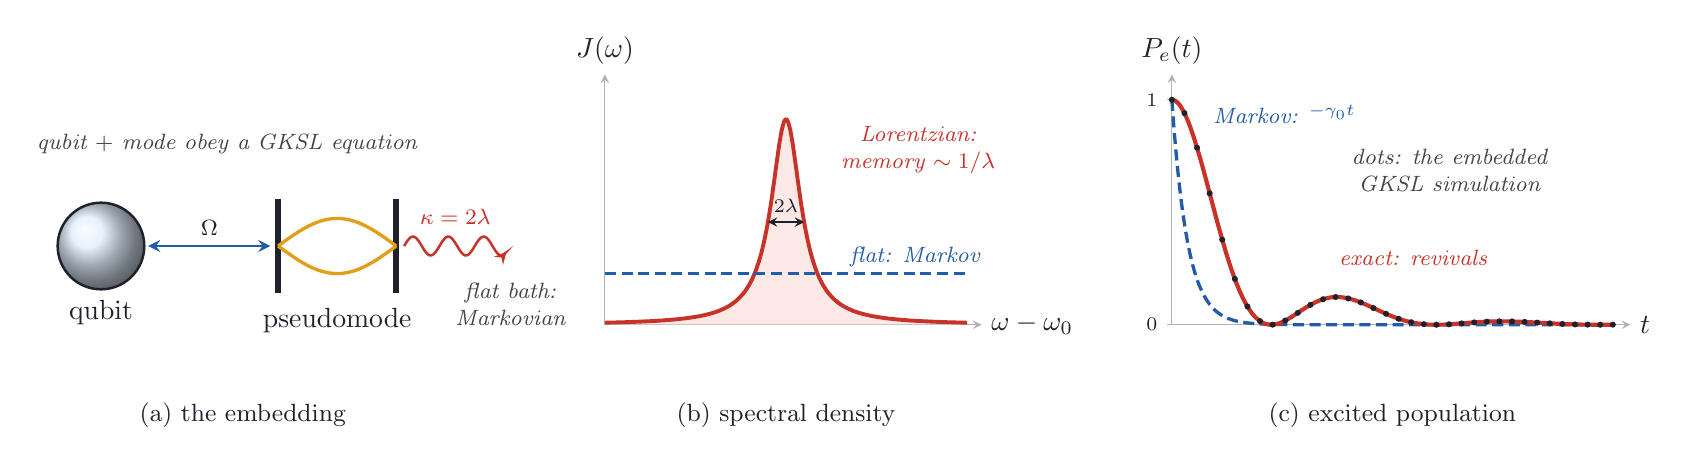
\begin{tikzpicture}[ink/.style={line width=0.9pt, ndInk}, faint/.style={line width=0.4pt, ndInk!35}, dashedink/.style={line width=0.5pt, ndInk!55, dash pattern=on 2.5pt off 2pt}, vec/.style={->, >=stealth, line width=1.2pt}, note/.style={font=\footnotesize\itshape, text=ndInk!85, align=center}, pointer/.style={->, >=stealth, line width=0.4pt, ndInk!60, shorten >=2pt, shorten <=1pt}, dot/.style={circle, fill=ndInk, inner sep=0pt, minimum size=3.4pt}, wash/.style={fill=ndSky, fill opacity=0.55}, every node/.style={text=ndInk}]
\definecolor{ndInk}{rgb}{0.13,0.13,0.18}
\definecolor{ndPaper}{rgb}{0.99,0.96,0.88}
\definecolor{ndSky}{rgb}{0.84,0.91,0.98}
\definecolor{ndRose}{rgb}{0.98,0.86,0.84}
\definecolor{ndBlue}{rgb}{0.13,0.36,0.66}
\definecolor{ndRed}{rgb}{0.78,0.20,0.16}
\definecolor{ndGold}{rgb}{0.88,0.62,0.10}
\definecolor{ndGreen}{rgb}{0.18,0.52,0.30}
\shade[ball color=ndSky!80!white] (0.000,0.000) circle (0.55);
\draw[ink] (0.000,0.000) circle (0.55);
\node at (0.000,-0.850) {qubit};
\draw[line width=2.2pt, ndInk] (2.250,-0.600) -- (2.250,0.600);
\draw[line width=2.2pt, ndInk] (3.750,-0.600) -- (3.750,0.600);
\draw[line width=1.2pt, ndGold] (2.250,0.000) -- (2.275,0.019) -- (2.301,0.037) -- (2.326,0.056) -- (2.352,0.074) -- (2.377,0.092) -- (2.403,0.110) -- (2.428,0.127) -- (2.453,0.145) -- (2.479,0.161) -- (2.504,0.178) -- (2.530,0.193) -- (2.555,0.209) -- (2.581,0.223) -- (2.606,0.237) -- (2.631,0.251) -- (2.657,0.263) -- (2.682,0.275) -- (2.708,0.286) -- (2.733,0.297) -- (2.758,0.306) -- (2.784,0.315) -- (2.809,0.322) -- (2.835,0.329) -- (2.860,0.335) -- (2.886,0.340) -- (2.911,0.344) -- (2.936,0.347) -- (2.962,0.349) -- (2.987,0.350) -- (3.013,0.350) -- (3.038,0.349) -- (3.064,0.347) -- (3.089,0.344) -- (3.114,0.340) -- (3.140,0.335) -- (3.165,0.329) -- (3.191,0.322) -- (3.216,0.315) -- (3.242,0.306) -- (3.267,0.297) -- (3.292,0.286) -- (3.318,0.275) -- (3.343,0.263) -- (3.369,0.251) -- (3.394,0.237) -- (3.419,0.223) -- (3.445,0.209) -- (3.470,0.193) -- (3.496,0.178) -- (3.521,0.161) -- (3.547,0.145) -- (3.572,0.127) -- (3.597,0.110) -- (3.623,0.092) -- (3.648,0.074) -- (3.674,0.056) -- (3.699,0.037) -- (3.725,0.019) -- (3.750,0.000);
\draw[line width=1.2pt, ndGold] (2.250,-0.000) -- (2.275,-0.019) -- (2.301,-0.037) -- (2.326,-0.056) -- (2.352,-0.074) -- (2.377,-0.092) -- (2.403,-0.110) -- (2.428,-0.127) -- (2.453,-0.145) -- (2.479,-0.161) -- (2.504,-0.178) -- (2.530,-0.193) -- (2.555,-0.209) -- (2.581,-0.223) -- (2.606,-0.237) -- (2.631,-0.251) -- (2.657,-0.263) -- (2.682,-0.275) -- (2.708,-0.286) -- (2.733,-0.297) -- (2.758,-0.306) -- (2.784,-0.315) -- (2.809,-0.322) -- (2.835,-0.329) -- (2.860,-0.335) -- (2.886,-0.340) -- (2.911,-0.344) -- (2.936,-0.347) -- (2.962,-0.349) -- (2.987,-0.350) -- (3.013,-0.350) -- (3.038,-0.349) -- (3.064,-0.347) -- (3.089,-0.344) -- (3.114,-0.340) -- (3.140,-0.335) -- (3.165,-0.329) -- (3.191,-0.322) -- (3.216,-0.315) -- (3.242,-0.306) -- (3.267,-0.297) -- (3.292,-0.286) -- (3.318,-0.275) -- (3.343,-0.263) -- (3.369,-0.251) -- (3.394,-0.237) -- (3.419,-0.223) -- (3.445,-0.209) -- (3.470,-0.193) -- (3.496,-0.178) -- (3.521,-0.161) -- (3.547,-0.145) -- (3.572,-0.127) -- (3.597,-0.110) -- (3.623,-0.092) -- (3.648,-0.074) -- (3.674,-0.056) -- (3.699,-0.037) -- (3.725,-0.019) -- (3.750,-0.000);
\node at (3.000,-0.950) {pseudomode};
\draw[<->, >=stealth, line width=0.9pt, ndBlue] (0.600,0.000) -- (2.150,0.000) node[midway, above, font=\footnotesize] {$\Omega$};
\draw[->, >=stealth, line width=0.9pt, ndRed] (3.850,0.000) -- (3.872,0.036) -- (3.894,0.069) -- (3.916,0.096) -- (3.938,0.113) -- (3.960,0.120) -- (3.982,0.115) -- (4.004,0.100) -- (4.026,0.075) -- (4.048,0.043) -- (4.070,0.007) -- (4.092,-0.030) -- (4.114,-0.064) -- (4.136,-0.092) -- (4.158,-0.111) -- (4.181,-0.120) -- (4.203,-0.117) -- (4.225,-0.103) -- (4.247,-0.080) -- (4.269,-0.049) -- (4.291,-0.014) -- (4.313,0.023) -- (4.335,0.058) -- (4.357,0.087) -- (4.379,0.108) -- (4.401,0.119) -- (4.423,0.118) -- (4.445,0.107) -- (4.467,0.085) -- (4.489,0.055) -- (4.511,0.020) -- (4.533,-0.016) -- (4.555,-0.052) -- (4.577,-0.082) -- (4.599,-0.105) -- (4.621,-0.118) -- (4.643,-0.119) -- (4.665,-0.110) -- (4.687,-0.090) -- (4.709,-0.061) -- (4.731,-0.027) -- (4.753,0.010) -- (4.775,0.046) -- (4.797,0.077) -- (4.819,0.101) -- (4.842,0.116) -- (4.864,0.120) -- (4.886,0.112) -- (4.908,0.094) -- (4.930,0.067) -- (4.952,0.034) -- (4.974,-0.003) -- (4.996,-0.039) -- (5.018,-0.072) -- (5.040,-0.098) -- (5.062,-0.114) -- (5.084,-0.120) -- (5.106,-0.114) -- (5.128,-0.098) -- (5.150,-0.073);
\node[font=\footnotesize, text=ndRed, above] at (4.500,0.150) {$\kappa=2\lambda$};
\node[note, anchor=north] at (5.200,-0.350) {flat bath:\\ Markovian};
\node[note, anchor=south] at (1.600,1.050) {qubit $+$ mode obey a GKSL equation};
\node[font=\small] at (1.8,-2.15) {(a) the embedding};
\draw[faint, ->, >=stealth] (6.400,-1.000) -- (11.184,-1.000) node[right, text=ndInk] {$\omega-\omega_0$};
\draw[faint, ->, >=stealth] (6.400,-1.000) -- (6.400,2.180) node[above, text=ndInk] {$J(\omega)$};
\fill[ndRose, fill opacity=0.6] (6.400,-1.000) -- (6.400,-0.974) -- (6.415,-0.974) -- (6.431,-0.973) -- (6.446,-0.973) -- (6.462,-0.973) -- (6.477,-0.972) -- (6.492,-0.972) -- (6.508,-0.972) -- (6.523,-0.971) -- (6.538,-0.971) -- (6.554,-0.970) -- (6.569,-0.970) -- (6.585,-0.970) -- (6.600,-0.969) -- (6.615,-0.969) -- (6.631,-0.968) -- (6.646,-0.968) -- (6.662,-0.967) -- (6.677,-0.967) -- (6.692,-0.966) -- (6.708,-0.966) -- (6.723,-0.965) -- (6.738,-0.965) -- (6.754,-0.964) -- (6.769,-0.963) -- (6.785,-0.963) -- (6.800,-0.962) -- (6.815,-0.962) -- (6.831,-0.961) -- (6.846,-0.960) -- (6.862,-0.960) -- (6.877,-0.959) -- (6.892,-0.958) -- (6.908,-0.958) -- (6.923,-0.957) -- (6.938,-0.956) -- (6.954,-0.956) -- (6.969,-0.955) -- (6.985,-0.954) -- (7.000,-0.953) -- (7.015,-0.952) -- (7.031,-0.951) -- (7.046,-0.951) -- (7.062,-0.950) -- (7.077,-0.949) -- (7.092,-0.948) -- (7.108,-0.947) -- (7.123,-0.946) -- (7.138,-0.945) -- (7.154,-0.944) -- (7.169,-0.942) -- (7.185,-0.941) -- (7.200,-0.940) -- (7.215,-0.939) -- (7.231,-0.938) -- (7.246,-0.936) -- (7.262,-0.935) -- (7.277,-0.934) -- (7.292,-0.932) -- (7.308,-0.931) -- (7.323,-0.929) -- (7.338,-0.928) -- (7.354,-0.926) -- (7.369,-0.924) -- (7.385,-0.923) -- (7.400,-0.921) -- (7.415,-0.919) -- (7.431,-0.917) -- (7.446,-0.915) -- (7.462,-0.913) -- (7.477,-0.911) -- (7.492,-0.909) -- (7.508,-0.906) -- (7.523,-0.904) -- (7.538,-0.902) -- (7.554,-0.899) -- (7.569,-0.896) -- (7.585,-0.894) -- (7.600,-0.891) -- (7.615,-0.888) -- (7.631,-0.885) -- (7.646,-0.881) -- (7.662,-0.878) -- (7.677,-0.874) -- (7.692,-0.871) -- (7.708,-0.867) -- (7.723,-0.863) -- (7.738,-0.859) -- (7.754,-0.854) -- (7.769,-0.850) -- (7.785,-0.845) -- (7.800,-0.840) -- (7.815,-0.835) -- (7.831,-0.829) -- (7.846,-0.824) -- (7.862,-0.817) -- (7.877,-0.811) -- (7.892,-0.804) -- (7.908,-0.797) -- (7.923,-0.790) -- (7.938,-0.782) -- (7.954,-0.774) -- (7.969,-0.765) -- (7.985,-0.756) -- (8.000,-0.746) -- (8.015,-0.735) -- (8.031,-0.724) -- (8.046,-0.713) -- (8.062,-0.700) -- (8.077,-0.687) -- (8.092,-0.673) -- (8.108,-0.658) -- (8.123,-0.642) -- (8.138,-0.625) -- (8.154,-0.607) -- (8.169,-0.588) -- (8.185,-0.567) -- (8.200,-0.544) -- (8.215,-0.520) -- (8.231,-0.495) -- (8.246,-0.467) -- (8.262,-0.437) -- (8.277,-0.405) -- (8.292,-0.370) -- (8.308,-0.333) -- (8.323,-0.292) -- (8.338,-0.248) -- (8.354,-0.201) -- (8.369,-0.150) -- (8.385,-0.094) -- (8.400,-0.034) -- (8.415,0.031) -- (8.431,0.101) -- (8.446,0.176) -- (8.462,0.257) -- (8.477,0.344) -- (8.492,0.437) -- (8.508,0.535) -- (8.523,0.639) -- (8.538,0.747) -- (8.554,0.858) -- (8.569,0.971) -- (8.585,1.084) -- (8.600,1.194) -- (8.615,1.298) -- (8.631,1.392) -- (8.646,1.473) -- (8.662,1.538) -- (8.677,1.583) -- (8.692,1.606) -- (8.708,1.606) -- (8.723,1.583) -- (8.738,1.538) -- (8.754,1.473) -- (8.769,1.392) -- (8.785,1.298) -- (8.800,1.194) -- (8.815,1.084) -- (8.831,0.971) -- (8.846,0.858) -- (8.862,0.747) -- (8.877,0.639) -- (8.892,0.535) -- (8.908,0.437) -- (8.923,0.344) -- (8.938,0.257) -- (8.954,0.176) -- (8.969,0.101) -- (8.985,0.031) -- (9.000,-0.034) -- (9.015,-0.094) -- (9.031,-0.150) -- (9.046,-0.201) -- (9.062,-0.248) -- (9.077,-0.292) -- (9.092,-0.333) -- (9.108,-0.370) -- (9.123,-0.405) -- (9.138,-0.437) -- (9.154,-0.467) -- (9.169,-0.495) -- (9.185,-0.520) -- (9.200,-0.544) -- (9.215,-0.567) -- (9.231,-0.588) -- (9.246,-0.607) -- (9.262,-0.625) -- (9.277,-0.642) -- (9.292,-0.658) -- (9.308,-0.673) -- (9.323,-0.687) -- (9.338,-0.700) -- (9.354,-0.713) -- (9.369,-0.724) -- (9.385,-0.735) -- (9.400,-0.746) -- (9.415,-0.756) -- (9.431,-0.765) -- (9.446,-0.774) -- (9.462,-0.782) -- (9.477,-0.790) -- (9.492,-0.797) -- (9.508,-0.804) -- (9.523,-0.811) -- (9.538,-0.817) -- (9.554,-0.824) -- (9.569,-0.829) -- (9.585,-0.835) -- (9.600,-0.840) -- (9.615,-0.845) -- (9.631,-0.850) -- (9.646,-0.854) -- (9.662,-0.859) -- (9.677,-0.863) -- (9.692,-0.867) -- (9.708,-0.871) -- (9.723,-0.874) -- (9.738,-0.878) -- (9.754,-0.881) -- (9.769,-0.885) -- (9.785,-0.888) -- (9.800,-0.891) -- (9.815,-0.894) -- (9.831,-0.896) -- (9.846,-0.899) -- (9.862,-0.902) -- (9.877,-0.904) -- (9.892,-0.906) -- (9.908,-0.909) -- (9.923,-0.911) -- (9.938,-0.913) -- (9.954,-0.915) -- (9.969,-0.917) -- (9.985,-0.919) -- (10.000,-0.921) -- (10.015,-0.923) -- (10.031,-0.924) -- (10.046,-0.926) -- (10.062,-0.928) -- (10.077,-0.929) -- (10.092,-0.931) -- (10.108,-0.932) -- (10.123,-0.934) -- (10.138,-0.935) -- (10.154,-0.936) -- (10.169,-0.938) -- (10.185,-0.939) -- (10.200,-0.940) -- (10.215,-0.941) -- (10.231,-0.942) -- (10.246,-0.944) -- (10.262,-0.945) -- (10.277,-0.946) -- (10.292,-0.947) -- (10.308,-0.948) -- (10.323,-0.949) -- (10.338,-0.950) -- (10.354,-0.951) -- (10.369,-0.951) -- (10.385,-0.952) -- (10.400,-0.953) -- (10.415,-0.954) -- (10.431,-0.955) -- (10.446,-0.956) -- (10.462,-0.956) -- (10.477,-0.957) -- (10.492,-0.958) -- (10.508,-0.958) -- (10.523,-0.959) -- (10.538,-0.960) -- (10.554,-0.960) -- (10.569,-0.961) -- (10.585,-0.962) -- (10.600,-0.962) -- (10.615,-0.963) -- (10.631,-0.963) -- (10.646,-0.964) -- (10.662,-0.965) -- (10.677,-0.965) -- (10.692,-0.966) -- (10.708,-0.966) -- (10.723,-0.967) -- (10.738,-0.967) -- (10.754,-0.968) -- (10.769,-0.968) -- (10.785,-0.969) -- (10.800,-0.969) -- (10.815,-0.970) -- (10.831,-0.970) -- (10.846,-0.970) -- (10.862,-0.971) -- (10.877,-0.971) -- (10.892,-0.972) -- (10.908,-0.972) -- (10.923,-0.972) -- (10.938,-0.973) -- (10.954,-0.973) -- (10.969,-0.973) -- (10.985,-0.974) -- (11.000,-0.974) -- (11.000,-1.000) -- cycle;
\draw[line width=1.4pt, ndRed] (6.400,-0.974) -- (6.415,-0.974) -- (6.431,-0.973) -- (6.446,-0.973) -- (6.462,-0.973) -- (6.477,-0.972) -- (6.492,-0.972) -- (6.508,-0.972) -- (6.523,-0.971) -- (6.538,-0.971) -- (6.554,-0.970) -- (6.569,-0.970) -- (6.585,-0.970) -- (6.600,-0.969) -- (6.615,-0.969) -- (6.631,-0.968) -- (6.646,-0.968) -- (6.662,-0.967) -- (6.677,-0.967) -- (6.692,-0.966) -- (6.708,-0.966) -- (6.723,-0.965) -- (6.738,-0.965) -- (6.754,-0.964) -- (6.769,-0.963) -- (6.785,-0.963) -- (6.800,-0.962) -- (6.815,-0.962) -- (6.831,-0.961) -- (6.846,-0.960) -- (6.862,-0.960) -- (6.877,-0.959) -- (6.892,-0.958) -- (6.908,-0.958) -- (6.923,-0.957) -- (6.938,-0.956) -- (6.954,-0.956) -- (6.969,-0.955) -- (6.985,-0.954) -- (7.000,-0.953) -- (7.015,-0.952) -- (7.031,-0.951) -- (7.046,-0.951) -- (7.062,-0.950) -- (7.077,-0.949) -- (7.092,-0.948) -- (7.108,-0.947) -- (7.123,-0.946) -- (7.138,-0.945) -- (7.154,-0.944) -- (7.169,-0.942) -- (7.185,-0.941) -- (7.200,-0.940) -- (7.215,-0.939) -- (7.231,-0.938) -- (7.246,-0.936) -- (7.262,-0.935) -- (7.277,-0.934) -- (7.292,-0.932) -- (7.308,-0.931) -- (7.323,-0.929) -- (7.338,-0.928) -- (7.354,-0.926) -- (7.369,-0.924) -- (7.385,-0.923) -- (7.400,-0.921) -- (7.415,-0.919) -- (7.431,-0.917) -- (7.446,-0.915) -- (7.462,-0.913) -- (7.477,-0.911) -- (7.492,-0.909) -- (7.508,-0.906) -- (7.523,-0.904) -- (7.538,-0.902) -- (7.554,-0.899) -- (7.569,-0.896) -- (7.585,-0.894) -- (7.600,-0.891) -- (7.615,-0.888) -- (7.631,-0.885) -- (7.646,-0.881) -- (7.662,-0.878) -- (7.677,-0.874) -- (7.692,-0.871) -- (7.708,-0.867) -- (7.723,-0.863) -- (7.738,-0.859) -- (7.754,-0.854) -- (7.769,-0.850) -- (7.785,-0.845) -- (7.800,-0.840) -- (7.815,-0.835) -- (7.831,-0.829) -- (7.846,-0.824) -- (7.862,-0.817) -- (7.877,-0.811) -- (7.892,-0.804) -- (7.908,-0.797) -- (7.923,-0.790) -- (7.938,-0.782) -- (7.954,-0.774) -- (7.969,-0.765) -- (7.985,-0.756) -- (8.000,-0.746) -- (8.015,-0.735) -- (8.031,-0.724) -- (8.046,-0.713) -- (8.062,-0.700) -- (8.077,-0.687) -- (8.092,-0.673) -- (8.108,-0.658) -- (8.123,-0.642) -- (8.138,-0.625) -- (8.154,-0.607) -- (8.169,-0.588) -- (8.185,-0.567) -- (8.200,-0.544) -- (8.215,-0.520) -- (8.231,-0.495) -- (8.246,-0.467) -- (8.262,-0.437) -- (8.277,-0.405) -- (8.292,-0.370) -- (8.308,-0.333) -- (8.323,-0.292) -- (8.338,-0.248) -- (8.354,-0.201) -- (8.369,-0.150) -- (8.385,-0.094) -- (8.400,-0.034) -- (8.415,0.031) -- (8.431,0.101) -- (8.446,0.176) -- (8.462,0.257) -- (8.477,0.344) -- (8.492,0.437) -- (8.508,0.535) -- (8.523,0.639) -- (8.538,0.747) -- (8.554,0.858) -- (8.569,0.971) -- (8.585,1.084) -- (8.600,1.194) -- (8.615,1.298) -- (8.631,1.392) -- (8.646,1.473) -- (8.662,1.538) -- (8.677,1.583) -- (8.692,1.606) -- (8.708,1.606) -- (8.723,1.583) -- (8.738,1.538) -- (8.754,1.473) -- (8.769,1.392) -- (8.785,1.298) -- (8.800,1.194) -- (8.815,1.084) -- (8.831,0.971) -- (8.846,0.858) -- (8.862,0.747) -- (8.877,0.639) -- (8.892,0.535) -- (8.908,0.437) -- (8.923,0.344) -- (8.938,0.257) -- (8.954,0.176) -- (8.969,0.101) -- (8.985,0.031) -- (9.000,-0.034) -- (9.015,-0.094) -- (9.031,-0.150) -- (9.046,-0.201) -- (9.062,-0.248) -- (9.077,-0.292) -- (9.092,-0.333) -- (9.108,-0.370) -- (9.123,-0.405) -- (9.138,-0.437) -- (9.154,-0.467) -- (9.169,-0.495) -- (9.185,-0.520) -- (9.200,-0.544) -- (9.215,-0.567) -- (9.231,-0.588) -- (9.246,-0.607) -- (9.262,-0.625) -- (9.277,-0.642) -- (9.292,-0.658) -- (9.308,-0.673) -- (9.323,-0.687) -- (9.338,-0.700) -- (9.354,-0.713) -- (9.369,-0.724) -- (9.385,-0.735) -- (9.400,-0.746) -- (9.415,-0.756) -- (9.431,-0.765) -- (9.446,-0.774) -- (9.462,-0.782) -- (9.477,-0.790) -- (9.492,-0.797) -- (9.508,-0.804) -- (9.523,-0.811) -- (9.538,-0.817) -- (9.554,-0.824) -- (9.569,-0.829) -- (9.585,-0.835) -- (9.600,-0.840) -- (9.615,-0.845) -- (9.631,-0.850) -- (9.646,-0.854) -- (9.662,-0.859) -- (9.677,-0.863) -- (9.692,-0.867) -- (9.708,-0.871) -- (9.723,-0.874) -- (9.738,-0.878) -- (9.754,-0.881) -- (9.769,-0.885) -- (9.785,-0.888) -- (9.800,-0.891) -- (9.815,-0.894) -- (9.831,-0.896) -- (9.846,-0.899) -- (9.862,-0.902) -- (9.877,-0.904) -- (9.892,-0.906) -- (9.908,-0.909) -- (9.923,-0.911) -- (9.938,-0.913) -- (9.954,-0.915) -- (9.969,-0.917) -- (9.985,-0.919) -- (10.000,-0.921) -- (10.015,-0.923) -- (10.031,-0.924) -- (10.046,-0.926) -- (10.062,-0.928) -- (10.077,-0.929) -- (10.092,-0.931) -- (10.108,-0.932) -- (10.123,-0.934) -- (10.138,-0.935) -- (10.154,-0.936) -- (10.169,-0.938) -- (10.185,-0.939) -- (10.200,-0.940) -- (10.215,-0.941) -- (10.231,-0.942) -- (10.246,-0.944) -- (10.262,-0.945) -- (10.277,-0.946) -- (10.292,-0.947) -- (10.308,-0.948) -- (10.323,-0.949) -- (10.338,-0.950) -- (10.354,-0.951) -- (10.369,-0.951) -- (10.385,-0.952) -- (10.400,-0.953) -- (10.415,-0.954) -- (10.431,-0.955) -- (10.446,-0.956) -- (10.462,-0.956) -- (10.477,-0.957) -- (10.492,-0.958) -- (10.508,-0.958) -- (10.523,-0.959) -- (10.538,-0.960) -- (10.554,-0.960) -- (10.569,-0.961) -- (10.585,-0.962) -- (10.600,-0.962) -- (10.615,-0.963) -- (10.631,-0.963) -- (10.646,-0.964) -- (10.662,-0.965) -- (10.677,-0.965) -- (10.692,-0.966) -- (10.708,-0.966) -- (10.723,-0.967) -- (10.738,-0.967) -- (10.754,-0.968) -- (10.769,-0.968) -- (10.785,-0.969) -- (10.800,-0.969) -- (10.815,-0.970) -- (10.831,-0.970) -- (10.846,-0.970) -- (10.862,-0.971) -- (10.877,-0.971) -- (10.892,-0.972) -- (10.908,-0.972) -- (10.923,-0.972) -- (10.938,-0.973) -- (10.954,-0.973) -- (10.969,-0.973) -- (10.985,-0.974) -- (11.000,-0.974);
\draw[line width=1.2pt, ndBlue, dash pattern=on 4pt off 2pt] (6.400,-0.348) -- (11.000,-0.348);
\draw[<->, >=stealth, ndInk, line width=0.5pt] (8.470,0.304) -- (8.930,0.304) node[midway, above, font=\scriptsize] {$2\lambda$};
\node[note, anchor=west, text=ndBlue] at (9.390,-0.139) {flat: Markov};
\node[note, anchor=west, text=ndRed] at (9.275,1.217) {Lorentzian:\\ memory $\sim1/\lambda$};
\node[font=\small] at (8.700,-2.150) {(b) spectral density};
\draw[faint, ->, >=stealth] (13.600,-1.000) -- (19.424,-1.000) node[right, text=ndInk] {$t$};
\draw[faint, ->, >=stealth] (13.600,-1.000) -- (13.600,2.180) node[above, text=ndInk] {$P_e(t)$};
\draw[faint] (13.660,-1.000) -- (13.540,-1.000) node[left, font=\scriptsize, text=ndInk] {$0$};
\draw[faint] (13.660,1.857) -- (13.540,1.857) node[left, font=\scriptsize, text=ndInk] {$1$};
\draw[line width=1.2pt, ndBlue, dash pattern=on 4pt off 2pt] (13.600,1.857) -- (13.608,1.745) -- (13.616,1.637) -- (13.624,1.534) -- (13.632,1.434) -- (13.640,1.339) -- (13.648,1.247) -- (13.656,1.159) -- (13.664,1.074) -- (13.672,0.992) -- (13.680,0.914) -- (13.688,0.839) -- (13.696,0.767) -- (13.704,0.697) -- (13.712,0.631) -- (13.720,0.567) -- (13.728,0.505) -- (13.736,0.446) -- (13.744,0.389) -- (13.752,0.335) -- (13.760,0.282) -- (13.768,0.232) -- (13.776,0.184) -- (13.784,0.137) -- (13.792,0.092) -- (13.800,0.050) -- (13.808,0.008) -- (13.816,-0.031) -- (13.824,-0.069) -- (13.832,-0.106) -- (13.840,-0.141) -- (13.848,-0.175) -- (13.856,-0.207) -- (13.864,-0.238) -- (13.872,-0.268) -- (13.880,-0.297) -- (13.888,-0.324) -- (13.896,-0.351) -- (13.904,-0.376) -- (13.912,-0.401) -- (13.920,-0.424) -- (13.928,-0.447) -- (13.936,-0.469) -- (13.944,-0.490) -- (13.953,-0.510) -- (13.961,-0.529) -- (13.969,-0.547) -- (13.977,-0.565) -- (13.985,-0.582) -- (13.993,-0.599) -- (14.001,-0.614) -- (14.009,-0.630) -- (14.017,-0.644) -- (14.025,-0.658) -- (14.033,-0.672) -- (14.041,-0.684) -- (14.049,-0.697) -- (14.057,-0.709) -- (14.065,-0.720) -- (14.073,-0.731) -- (14.081,-0.742) -- (14.089,-0.752) -- (14.097,-0.762) -- (14.105,-0.771) -- (14.113,-0.780) -- (14.121,-0.789) -- (14.129,-0.797) -- (14.137,-0.805) -- (14.145,-0.813) -- (14.153,-0.820) -- (14.161,-0.827) -- (14.169,-0.834) -- (14.177,-0.840) -- (14.185,-0.847) -- (14.193,-0.853) -- (14.201,-0.858) -- (14.209,-0.864) -- (14.217,-0.869) -- (14.225,-0.874) -- (14.233,-0.879) -- (14.241,-0.884) -- (14.249,-0.889) -- (14.257,-0.893) -- (14.265,-0.897) -- (14.273,-0.901) -- (14.281,-0.905) -- (14.289,-0.909) -- (14.297,-0.912) -- (14.305,-0.916) -- (14.313,-0.919) -- (14.321,-0.922) -- (14.329,-0.925) -- (14.337,-0.928) -- (14.345,-0.931) -- (14.353,-0.934) -- (14.361,-0.936) -- (14.369,-0.939) -- (14.377,-0.941) -- (14.385,-0.944) -- (14.393,-0.946) -- (14.401,-0.948) -- (14.409,-0.950) -- (14.417,-0.952) -- (14.425,-0.954) -- (14.433,-0.956) -- (14.441,-0.957) -- (14.449,-0.959) -- (14.457,-0.961) -- (14.465,-0.962) -- (14.473,-0.964) -- (14.481,-0.965) -- (14.489,-0.967) -- (14.497,-0.968) -- (14.505,-0.969) -- (14.513,-0.970) -- (14.521,-0.971) -- (14.529,-0.973) -- (14.537,-0.974) -- (14.545,-0.975) -- (14.553,-0.976) -- (14.561,-0.977) -- (14.569,-0.978) -- (14.577,-0.978) -- (14.585,-0.979) -- (14.593,-0.980) -- (14.601,-0.981) -- (14.609,-0.982) -- (14.617,-0.982) -- (14.625,-0.983) -- (14.633,-0.984) -- (14.641,-0.984) -- (14.649,-0.985) -- (14.658,-0.986) -- (14.666,-0.986) -- (14.674,-0.987) -- (14.682,-0.987) -- (14.690,-0.988) -- (14.698,-0.988) -- (14.706,-0.989) -- (14.714,-0.989) -- (14.722,-0.990) -- (14.730,-0.990) -- (14.738,-0.990) -- (14.746,-0.991) -- (14.754,-0.991) -- (14.762,-0.991) -- (14.770,-0.992) -- (14.778,-0.992) -- (14.786,-0.992) -- (14.794,-0.993) -- (14.802,-0.993) -- (14.810,-0.993) -- (14.818,-0.994) -- (14.826,-0.994) -- (14.834,-0.994) -- (14.842,-0.994) -- (14.850,-0.994) -- (14.858,-0.995) -- (14.866,-0.995) -- (14.874,-0.995) -- (14.882,-0.995) -- (14.890,-0.995) -- (14.898,-0.996) -- (14.906,-0.996) -- (14.914,-0.996) -- (14.922,-0.996) -- (14.930,-0.996) -- (14.938,-0.996) -- (14.946,-0.997) -- (14.954,-0.997) -- (14.962,-0.997) -- (14.970,-0.997) -- (14.978,-0.997) -- (14.986,-0.997) -- (14.994,-0.997) -- (15.002,-0.997) -- (15.010,-0.998) -- (15.018,-0.998) -- (15.026,-0.998) -- (15.034,-0.998) -- (15.042,-0.998) -- (15.050,-0.998) -- (15.058,-0.998) -- (15.066,-0.998) -- (15.074,-0.998) -- (15.082,-0.998) -- (15.090,-0.998) -- (15.098,-0.998) -- (15.106,-0.998) -- (15.114,-0.999) -- (15.122,-0.999) -- (15.130,-0.999) -- (15.138,-0.999) -- (15.146,-0.999) -- (15.154,-0.999) -- (15.162,-0.999) -- (15.170,-0.999) -- (15.178,-0.999) -- (15.186,-0.999) -- (15.194,-0.999) -- (15.202,-0.999) -- (15.210,-0.999) -- (15.218,-0.999) -- (15.226,-0.999) -- (15.234,-0.999) -- (15.242,-0.999) -- (15.250,-0.999) -- (15.258,-0.999) -- (15.266,-0.999) -- (15.274,-0.999) -- (15.282,-0.999) -- (15.290,-0.999) -- (15.298,-0.999) -- (15.306,-0.999) -- (15.314,-0.999) -- (15.322,-0.999) -- (15.330,-1.000) -- (15.338,-1.000) -- (15.346,-1.000) -- (15.355,-1.000) -- (15.363,-1.000) -- (15.371,-1.000) -- (15.379,-1.000) -- (15.387,-1.000) -- (15.395,-1.000) -- (15.403,-1.000) -- (15.411,-1.000) -- (15.419,-1.000) -- (15.427,-1.000) -- (15.435,-1.000) -- (15.443,-1.000) -- (15.451,-1.000) -- (15.459,-1.000) -- (15.467,-1.000) -- (15.475,-1.000) -- (15.483,-1.000) -- (15.491,-1.000) -- (15.499,-1.000) -- (15.507,-1.000) -- (15.515,-1.000) -- (15.523,-1.000) -- (15.531,-1.000) -- (15.539,-1.000) -- (15.547,-1.000) -- (15.555,-1.000) -- (15.563,-1.000) -- (15.571,-1.000) -- (15.579,-1.000) -- (15.587,-1.000) -- (15.595,-1.000) -- (15.603,-1.000) -- (15.611,-1.000) -- (15.619,-1.000) -- (15.627,-1.000) -- (15.635,-1.000) -- (15.643,-1.000) -- (15.651,-1.000) -- (15.659,-1.000) -- (15.667,-1.000) -- (15.675,-1.000) -- (15.683,-1.000) -- (15.691,-1.000) -- (15.699,-1.000) -- (15.707,-1.000) -- (15.715,-1.000) -- (15.723,-1.000) -- (15.731,-1.000) -- (15.739,-1.000) -- (15.747,-1.000) -- (15.755,-1.000) -- (15.763,-1.000) -- (15.771,-1.000) -- (15.779,-1.000) -- (15.787,-1.000) -- (15.795,-1.000) -- (15.803,-1.000) -- (15.811,-1.000) -- (15.819,-1.000) -- (15.827,-1.000) -- (15.835,-1.000) -- (15.843,-1.000) -- (15.851,-1.000) -- (15.859,-1.000) -- (15.867,-1.000) -- (15.875,-1.000) -- (15.883,-1.000) -- (15.891,-1.000) -- (15.899,-1.000) -- (15.907,-1.000) -- (15.915,-1.000) -- (15.923,-1.000) -- (15.931,-1.000) -- (15.939,-1.000) -- (15.947,-1.000) -- (15.955,-1.000) -- (15.963,-1.000) -- (15.971,-1.000) -- (15.979,-1.000) -- (15.987,-1.000) -- (15.995,-1.000) -- (16.003,-1.000) -- (16.011,-1.000) -- (16.019,-1.000) -- (16.027,-1.000) -- (16.035,-1.000) -- (16.043,-1.000) -- (16.052,-1.000) -- (16.060,-1.000) -- (16.068,-1.000) -- (16.076,-1.000) -- (16.084,-1.000) -- (16.092,-1.000) -- (16.100,-1.000) -- (16.108,-1.000) -- (16.116,-1.000) -- (16.124,-1.000) -- (16.132,-1.000) -- (16.140,-1.000) -- (16.148,-1.000) -- (16.156,-1.000) -- (16.164,-1.000) -- (16.172,-1.000) -- (16.180,-1.000) -- (16.188,-1.000) -- (16.196,-1.000) -- (16.204,-1.000) -- (16.212,-1.000) -- (16.220,-1.000) -- (16.228,-1.000) -- (16.236,-1.000) -- (16.244,-1.000) -- (16.252,-1.000) -- (16.260,-1.000) -- (16.268,-1.000) -- (16.276,-1.000) -- (16.284,-1.000) -- (16.292,-1.000) -- (16.300,-1.000) -- (16.308,-1.000) -- (16.316,-1.000) -- (16.324,-1.000) -- (16.332,-1.000) -- (16.340,-1.000) -- (16.348,-1.000) -- (16.356,-1.000) -- (16.364,-1.000) -- (16.372,-1.000) -- (16.380,-1.000) -- (16.388,-1.000) -- (16.396,-1.000) -- (16.404,-1.000) -- (16.412,-1.000) -- (16.420,-1.000) -- (16.428,-1.000) -- (16.436,-1.000) -- (16.444,-1.000) -- (16.452,-1.000) -- (16.460,-1.000) -- (16.468,-1.000) -- (16.476,-1.000) -- (16.484,-1.000) -- (16.492,-1.000) -- (16.500,-1.000) -- (16.508,-1.000) -- (16.516,-1.000) -- (16.524,-1.000) -- (16.532,-1.000) -- (16.540,-1.000) -- (16.548,-1.000) -- (16.556,-1.000) -- (16.564,-1.000) -- (16.572,-1.000) -- (16.580,-1.000) -- (16.588,-1.000) -- (16.596,-1.000) -- (16.604,-1.000) -- (16.612,-1.000) -- (16.620,-1.000) -- (16.628,-1.000) -- (16.636,-1.000) -- (16.644,-1.000) -- (16.652,-1.000) -- (16.660,-1.000) -- (16.668,-1.000) -- (16.676,-1.000) -- (16.684,-1.000) -- (16.692,-1.000) -- (16.700,-1.000) -- (16.708,-1.000) -- (16.716,-1.000) -- (16.724,-1.000) -- (16.732,-1.000) -- (16.740,-1.000) -- (16.748,-1.000) -- (16.757,-1.000) -- (16.765,-1.000) -- (16.773,-1.000) -- (16.781,-1.000) -- (16.789,-1.000) -- (16.797,-1.000) -- (16.805,-1.000) -- (16.813,-1.000) -- (16.821,-1.000) -- (16.829,-1.000) -- (16.837,-1.000) -- (16.845,-1.000) -- (16.853,-1.000) -- (16.861,-1.000) -- (16.869,-1.000) -- (16.877,-1.000) -- (16.885,-1.000) -- (16.893,-1.000) -- (16.901,-1.000) -- (16.909,-1.000) -- (16.917,-1.000) -- (16.925,-1.000) -- (16.933,-1.000) -- (16.941,-1.000) -- (16.949,-1.000) -- (16.957,-1.000) -- (16.965,-1.000) -- (16.973,-1.000) -- (16.981,-1.000) -- (16.989,-1.000) -- (16.997,-1.000) -- (17.005,-1.000) -- (17.013,-1.000) -- (17.021,-1.000) -- (17.029,-1.000) -- (17.037,-1.000) -- (17.045,-1.000) -- (17.053,-1.000) -- (17.061,-1.000) -- (17.069,-1.000) -- (17.077,-1.000) -- (17.085,-1.000) -- (17.093,-1.000) -- (17.101,-1.000) -- (17.109,-1.000) -- (17.117,-1.000) -- (17.125,-1.000) -- (17.133,-1.000) -- (17.141,-1.000) -- (17.149,-1.000) -- (17.157,-1.000) -- (17.165,-1.000) -- (17.173,-1.000) -- (17.181,-1.000) -- (17.189,-1.000) -- (17.197,-1.000) -- (17.205,-1.000) -- (17.213,-1.000) -- (17.221,-1.000) -- (17.229,-1.000) -- (17.237,-1.000) -- (17.245,-1.000) -- (17.253,-1.000) -- (17.261,-1.000) -- (17.269,-1.000) -- (17.277,-1.000) -- (17.285,-1.000) -- (17.293,-1.000) -- (17.301,-1.000) -- (17.309,-1.000) -- (17.317,-1.000) -- (17.325,-1.000) -- (17.333,-1.000) -- (17.341,-1.000) -- (17.349,-1.000) -- (17.357,-1.000) -- (17.365,-1.000) -- (17.373,-1.000) -- (17.381,-1.000) -- (17.389,-1.000) -- (17.397,-1.000) -- (17.405,-1.000) -- (17.413,-1.000) -- (17.421,-1.000) -- (17.429,-1.000) -- (17.437,-1.000) -- (17.445,-1.000) -- (17.454,-1.000) -- (17.462,-1.000) -- (17.470,-1.000) -- (17.478,-1.000) -- (17.486,-1.000) -- (17.494,-1.000) -- (17.502,-1.000) -- (17.510,-1.000) -- (17.518,-1.000) -- (17.526,-1.000) -- (17.534,-1.000) -- (17.542,-1.000) -- (17.550,-1.000) -- (17.558,-1.000) -- (17.566,-1.000) -- (17.574,-1.000) -- (17.582,-1.000) -- (17.590,-1.000) -- (17.598,-1.000) -- (17.606,-1.000) -- (17.614,-1.000) -- (17.622,-1.000) -- (17.630,-1.000) -- (17.638,-1.000) -- (17.646,-1.000) -- (17.654,-1.000) -- (17.662,-1.000) -- (17.670,-1.000) -- (17.678,-1.000) -- (17.686,-1.000) -- (17.694,-1.000) -- (17.702,-1.000) -- (17.710,-1.000) -- (17.718,-1.000) -- (17.726,-1.000) -- (17.734,-1.000) -- (17.742,-1.000) -- (17.750,-1.000) -- (17.758,-1.000) -- (17.766,-1.000) -- (17.774,-1.000) -- (17.782,-1.000) -- (17.790,-1.000) -- (17.798,-1.000) -- (17.806,-1.000) -- (17.814,-1.000) -- (17.822,-1.000) -- (17.830,-1.000) -- (17.838,-1.000) -- (17.846,-1.000) -- (17.854,-1.000) -- (17.862,-1.000) -- (17.870,-1.000) -- (17.878,-1.000) -- (17.886,-1.000) -- (17.894,-1.000) -- (17.902,-1.000) -- (17.910,-1.000) -- (17.918,-1.000) -- (17.926,-1.000) -- (17.934,-1.000) -- (17.942,-1.000) -- (17.950,-1.000) -- (17.958,-1.000) -- (17.966,-1.000) -- (17.974,-1.000) -- (17.982,-1.000) -- (17.990,-1.000) -- (17.998,-1.000) -- (18.006,-1.000) -- (18.014,-1.000) -- (18.022,-1.000) -- (18.030,-1.000) -- (18.038,-1.000) -- (18.046,-1.000) -- (18.054,-1.000) -- (18.062,-1.000) -- (18.070,-1.000) -- (18.078,-1.000) -- (18.086,-1.000) -- (18.094,-1.000) -- (18.102,-1.000) -- (18.110,-1.000) -- (18.118,-1.000) -- (18.126,-1.000) -- (18.134,-1.000) -- (18.142,-1.000) -- (18.151,-1.000) -- (18.159,-1.000) -- (18.167,-1.000) -- (18.175,-1.000) -- (18.183,-1.000) -- (18.191,-1.000) -- (18.199,-1.000) -- (18.207,-1.000) -- (18.215,-1.000) -- (18.223,-1.000) -- (18.231,-1.000) -- (18.239,-1.000) -- (18.247,-1.000) -- (18.255,-1.000) -- (18.263,-1.000) -- (18.271,-1.000) -- (18.279,-1.000) -- (18.287,-1.000) -- (18.295,-1.000) -- (18.303,-1.000) -- (18.311,-1.000) -- (18.319,-1.000) -- (18.327,-1.000) -- (18.335,-1.000) -- (18.343,-1.000) -- (18.351,-1.000) -- (18.359,-1.000) -- (18.367,-1.000) -- (18.375,-1.000) -- (18.383,-1.000) -- (18.391,-1.000) -- (18.399,-1.000) -- (18.407,-1.000) -- (18.415,-1.000) -- (18.423,-1.000) -- (18.431,-1.000) -- (18.439,-1.000) -- (18.447,-1.000) -- (18.455,-1.000) -- (18.463,-1.000) -- (18.471,-1.000) -- (18.479,-1.000) -- (18.487,-1.000) -- (18.495,-1.000) -- (18.503,-1.000) -- (18.511,-1.000) -- (18.519,-1.000) -- (18.527,-1.000) -- (18.535,-1.000) -- (18.543,-1.000) -- (18.551,-1.000) -- (18.559,-1.000) -- (18.567,-1.000) -- (18.575,-1.000) -- (18.583,-1.000) -- (18.591,-1.000) -- (18.599,-1.000) -- (18.607,-1.000) -- (18.615,-1.000) -- (18.623,-1.000) -- (18.631,-1.000) -- (18.639,-1.000) -- (18.647,-1.000) -- (18.655,-1.000) -- (18.663,-1.000) -- (18.671,-1.000) -- (18.679,-1.000) -- (18.687,-1.000) -- (18.695,-1.000) -- (18.703,-1.000) -- (18.711,-1.000) -- (18.719,-1.000) -- (18.727,-1.000) -- (18.735,-1.000) -- (18.743,-1.000) -- (18.751,-1.000) -- (18.759,-1.000) -- (18.767,-1.000) -- (18.775,-1.000) -- (18.783,-1.000) -- (18.791,-1.000) -- (18.799,-1.000) -- (18.807,-1.000) -- (18.815,-1.000) -- (18.823,-1.000) -- (18.831,-1.000) -- (18.839,-1.000) -- (18.847,-1.000) -- (18.856,-1.000) -- (18.864,-1.000) -- (18.872,-1.000) -- (18.880,-1.000) -- (18.888,-1.000) -- (18.896,-1.000) -- (18.904,-1.000) -- (18.912,-1.000) -- (18.920,-1.000) -- (18.928,-1.000) -- (18.936,-1.000) -- (18.944,-1.000) -- (18.952,-1.000) -- (18.960,-1.000) -- (18.968,-1.000) -- (18.976,-1.000) -- (18.984,-1.000) -- (18.992,-1.000) -- (19.000,-1.000) -- (19.008,-1.000) -- (19.016,-1.000) -- (19.024,-1.000) -- (19.032,-1.000) -- (19.040,-1.000) -- (19.048,-1.000) -- (19.056,-1.000) -- (19.064,-1.000) -- (19.072,-1.000) -- (19.080,-1.000) -- (19.088,-1.000) -- (19.096,-1.000) -- (19.104,-1.000) -- (19.112,-1.000) -- (19.120,-1.000) -- (19.128,-1.000) -- (19.136,-1.000) -- (19.144,-1.000) -- (19.152,-1.000) -- (19.160,-1.000) -- (19.168,-1.000) -- (19.176,-1.000) -- (19.184,-1.000) -- (19.192,-1.000) -- (19.200,-1.000);
\draw[line width=1.5pt, ndRed] (13.600,1.857) -- (13.608,1.857) -- (13.616,1.855) -- (13.624,1.853) -- (13.632,1.850) -- (13.640,1.846) -- (13.648,1.841) -- (13.656,1.835) -- (13.664,1.829) -- (13.672,1.821) -- (13.680,1.813) -- (13.688,1.804) -- (13.696,1.794) -- (13.704,1.783) -- (13.712,1.771) -- (13.720,1.759) -- (13.728,1.746) -- (13.736,1.732) -- (13.744,1.718) -- (13.752,1.703) -- (13.760,1.687) -- (13.768,1.670) -- (13.776,1.653) -- (13.784,1.635) -- (13.792,1.616) -- (13.800,1.597) -- (13.808,1.577) -- (13.816,1.557) -- (13.824,1.536) -- (13.832,1.515) -- (13.840,1.493) -- (13.848,1.470) -- (13.856,1.447) -- (13.864,1.423) -- (13.872,1.399) -- (13.880,1.375) -- (13.888,1.350) -- (13.896,1.325) -- (13.904,1.299) -- (13.912,1.273) -- (13.920,1.246) -- (13.928,1.220) -- (13.936,1.192) -- (13.944,1.165) -- (13.953,1.137) -- (13.961,1.109) -- (13.969,1.081) -- (13.977,1.052) -- (13.985,1.024) -- (13.993,0.995) -- (14.001,0.965) -- (14.009,0.936) -- (14.017,0.906) -- (14.025,0.877) -- (14.033,0.847) -- (14.041,0.817) -- (14.049,0.787) -- (14.057,0.757) -- (14.065,0.727) -- (14.073,0.697) -- (14.081,0.666) -- (14.089,0.636) -- (14.097,0.606) -- (14.105,0.576) -- (14.113,0.545) -- (14.121,0.515) -- (14.129,0.485) -- (14.137,0.455) -- (14.145,0.425) -- (14.153,0.395) -- (14.161,0.365) -- (14.169,0.336) -- (14.177,0.306) -- (14.185,0.277) -- (14.193,0.248) -- (14.201,0.219) -- (14.209,0.190) -- (14.217,0.161) -- (14.225,0.133) -- (14.233,0.105) -- (14.241,0.077) -- (14.249,0.049) -- (14.257,0.021) -- (14.265,-0.006) -- (14.273,-0.033) -- (14.281,-0.060) -- (14.289,-0.086) -- (14.297,-0.112) -- (14.305,-0.138) -- (14.313,-0.163) -- (14.321,-0.189) -- (14.329,-0.214) -- (14.337,-0.238) -- (14.345,-0.262) -- (14.353,-0.286) -- (14.361,-0.310) -- (14.369,-0.333) -- (14.377,-0.355) -- (14.385,-0.378) -- (14.393,-0.400) -- (14.401,-0.422) -- (14.409,-0.443) -- (14.417,-0.464) -- (14.425,-0.484) -- (14.433,-0.504) -- (14.441,-0.524) -- (14.449,-0.543) -- (14.457,-0.562) -- (14.465,-0.581) -- (14.473,-0.599) -- (14.481,-0.616) -- (14.489,-0.633) -- (14.497,-0.650) -- (14.505,-0.667) -- (14.513,-0.683) -- (14.521,-0.698) -- (14.529,-0.713) -- (14.537,-0.728) -- (14.545,-0.742) -- (14.553,-0.756) -- (14.561,-0.770) -- (14.569,-0.783) -- (14.577,-0.796) -- (14.585,-0.808) -- (14.593,-0.820) -- (14.601,-0.831) -- (14.609,-0.842) -- (14.617,-0.853) -- (14.625,-0.863) -- (14.633,-0.873) -- (14.641,-0.882) -- (14.649,-0.891) -- (14.658,-0.900) -- (14.666,-0.908) -- (14.674,-0.916) -- (14.682,-0.923) -- (14.690,-0.930) -- (14.698,-0.937) -- (14.706,-0.943) -- (14.714,-0.949) -- (14.722,-0.955) -- (14.730,-0.960) -- (14.738,-0.965) -- (14.746,-0.970) -- (14.754,-0.974) -- (14.762,-0.978) -- (14.770,-0.981) -- (14.778,-0.985) -- (14.786,-0.987) -- (14.794,-0.990) -- (14.802,-0.992) -- (14.810,-0.994) -- (14.818,-0.996) -- (14.826,-0.997) -- (14.834,-0.998) -- (14.842,-0.999) -- (14.850,-1.000) -- (14.858,-1.000) -- (14.866,-1.000) -- (14.874,-1.000) -- (14.882,-0.999) -- (14.890,-0.998) -- (14.898,-0.997) -- (14.906,-0.996) -- (14.914,-0.995) -- (14.922,-0.993) -- (14.930,-0.991) -- (14.938,-0.989) -- (14.946,-0.987) -- (14.954,-0.984) -- (14.962,-0.982) -- (14.970,-0.979) -- (14.978,-0.976) -- (14.986,-0.973) -- (14.994,-0.969) -- (15.002,-0.966) -- (15.010,-0.962) -- (15.018,-0.958) -- (15.026,-0.955) -- (15.034,-0.951) -- (15.042,-0.946) -- (15.050,-0.942) -- (15.058,-0.938) -- (15.066,-0.933) -- (15.074,-0.929) -- (15.082,-0.924) -- (15.090,-0.919) -- (15.098,-0.914) -- (15.106,-0.910) -- (15.114,-0.905) -- (15.122,-0.900) -- (15.130,-0.894) -- (15.138,-0.889) -- (15.146,-0.884) -- (15.154,-0.879) -- (15.162,-0.874) -- (15.170,-0.868) -- (15.178,-0.863) -- (15.186,-0.858) -- (15.194,-0.852) -- (15.202,-0.847) -- (15.210,-0.842) -- (15.218,-0.836) -- (15.226,-0.831) -- (15.234,-0.826) -- (15.242,-0.821) -- (15.250,-0.815) -- (15.258,-0.810) -- (15.266,-0.805) -- (15.274,-0.800) -- (15.282,-0.795) -- (15.290,-0.789) -- (15.298,-0.784) -- (15.306,-0.779) -- (15.314,-0.774) -- (15.322,-0.770) -- (15.330,-0.765) -- (15.338,-0.760) -- (15.346,-0.755) -- (15.355,-0.751) -- (15.363,-0.746) -- (15.371,-0.742) -- (15.379,-0.737) -- (15.387,-0.733) -- (15.395,-0.729) -- (15.403,-0.725) -- (15.411,-0.721) -- (15.419,-0.717) -- (15.427,-0.713) -- (15.435,-0.709) -- (15.443,-0.706) -- (15.451,-0.702) -- (15.459,-0.699) -- (15.467,-0.695) -- (15.475,-0.692) -- (15.483,-0.689) -- (15.491,-0.686) -- (15.499,-0.683) -- (15.507,-0.680) -- (15.515,-0.677) -- (15.523,-0.675) -- (15.531,-0.672) -- (15.539,-0.670) -- (15.547,-0.668) -- (15.555,-0.666) -- (15.563,-0.664) -- (15.571,-0.662) -- (15.579,-0.660) -- (15.587,-0.659) -- (15.595,-0.657) -- (15.603,-0.656) -- (15.611,-0.654) -- (15.619,-0.653) -- (15.627,-0.652) -- (15.635,-0.651) -- (15.643,-0.651) -- (15.651,-0.650) -- (15.659,-0.649) -- (15.667,-0.649) -- (15.675,-0.648) -- (15.683,-0.648) -- (15.691,-0.648) -- (15.699,-0.648) -- (15.707,-0.648) -- (15.715,-0.649) -- (15.723,-0.649) -- (15.731,-0.649) -- (15.739,-0.650) -- (15.747,-0.651) -- (15.755,-0.651) -- (15.763,-0.652) -- (15.771,-0.653) -- (15.779,-0.654) -- (15.787,-0.655) -- (15.795,-0.657) -- (15.803,-0.658) -- (15.811,-0.660) -- (15.819,-0.661) -- (15.827,-0.663) -- (15.835,-0.665) -- (15.843,-0.666) -- (15.851,-0.668) -- (15.859,-0.670) -- (15.867,-0.672) -- (15.875,-0.675) -- (15.883,-0.677) -- (15.891,-0.679) -- (15.899,-0.682) -- (15.907,-0.684) -- (15.915,-0.687) -- (15.923,-0.689) -- (15.931,-0.692) -- (15.939,-0.695) -- (15.947,-0.697) -- (15.955,-0.700) -- (15.963,-0.703) -- (15.971,-0.706) -- (15.979,-0.709) -- (15.987,-0.712) -- (15.995,-0.716) -- (16.003,-0.719) -- (16.011,-0.722) -- (16.019,-0.725) -- (16.027,-0.729) -- (16.035,-0.732) -- (16.043,-0.735) -- (16.052,-0.739) -- (16.060,-0.742) -- (16.068,-0.746) -- (16.076,-0.749) -- (16.084,-0.753) -- (16.092,-0.756) -- (16.100,-0.760) -- (16.108,-0.764) -- (16.116,-0.767) -- (16.124,-0.771) -- (16.132,-0.775) -- (16.140,-0.778) -- (16.148,-0.782) -- (16.156,-0.786) -- (16.164,-0.789) -- (16.172,-0.793) -- (16.180,-0.797) -- (16.188,-0.801) -- (16.196,-0.804) -- (16.204,-0.808) -- (16.212,-0.812) -- (16.220,-0.816) -- (16.228,-0.819) -- (16.236,-0.823) -- (16.244,-0.827) -- (16.252,-0.830) -- (16.260,-0.834) -- (16.268,-0.838) -- (16.276,-0.841) -- (16.284,-0.845) -- (16.292,-0.848) -- (16.300,-0.852) -- (16.308,-0.856) -- (16.316,-0.859) -- (16.324,-0.863) -- (16.332,-0.866) -- (16.340,-0.869) -- (16.348,-0.873) -- (16.356,-0.876) -- (16.364,-0.879) -- (16.372,-0.883) -- (16.380,-0.886) -- (16.388,-0.889) -- (16.396,-0.892) -- (16.404,-0.896) -- (16.412,-0.899) -- (16.420,-0.902) -- (16.428,-0.905) -- (16.436,-0.908) -- (16.444,-0.911) -- (16.452,-0.914) -- (16.460,-0.917) -- (16.468,-0.919) -- (16.476,-0.922) -- (16.484,-0.925) -- (16.492,-0.928) -- (16.500,-0.930) -- (16.508,-0.933) -- (16.516,-0.935) -- (16.524,-0.938) -- (16.532,-0.940) -- (16.540,-0.943) -- (16.548,-0.945) -- (16.556,-0.947) -- (16.564,-0.950) -- (16.572,-0.952) -- (16.580,-0.954) -- (16.588,-0.956) -- (16.596,-0.958) -- (16.604,-0.960) -- (16.612,-0.962) -- (16.620,-0.964) -- (16.628,-0.966) -- (16.636,-0.968) -- (16.644,-0.969) -- (16.652,-0.971) -- (16.660,-0.973) -- (16.668,-0.974) -- (16.676,-0.976) -- (16.684,-0.977) -- (16.692,-0.979) -- (16.700,-0.980) -- (16.708,-0.981) -- (16.716,-0.983) -- (16.724,-0.984) -- (16.732,-0.985) -- (16.740,-0.986) -- (16.748,-0.987) -- (16.757,-0.988) -- (16.765,-0.989) -- (16.773,-0.990) -- (16.781,-0.991) -- (16.789,-0.992) -- (16.797,-0.993) -- (16.805,-0.993) -- (16.813,-0.994) -- (16.821,-0.995) -- (16.829,-0.995) -- (16.837,-0.996) -- (16.845,-0.997) -- (16.853,-0.997) -- (16.861,-0.998) -- (16.869,-0.998) -- (16.877,-0.998) -- (16.885,-0.999) -- (16.893,-0.999) -- (16.901,-0.999) -- (16.909,-0.999) -- (16.917,-1.000) -- (16.925,-1.000) -- (16.933,-1.000) -- (16.941,-1.000) -- (16.949,-1.000) -- (16.957,-1.000) -- (16.965,-1.000) -- (16.973,-1.000) -- (16.981,-1.000) -- (16.989,-1.000) -- (16.997,-1.000) -- (17.005,-0.999) -- (17.013,-0.999) -- (17.021,-0.999) -- (17.029,-0.999) -- (17.037,-0.999) -- (17.045,-0.998) -- (17.053,-0.998) -- (17.061,-0.998) -- (17.069,-0.997) -- (17.077,-0.997) -- (17.085,-0.996) -- (17.093,-0.996) -- (17.101,-0.996) -- (17.109,-0.995) -- (17.117,-0.995) -- (17.125,-0.994) -- (17.133,-0.994) -- (17.141,-0.993) -- (17.149,-0.993) -- (17.157,-0.992) -- (17.165,-0.991) -- (17.173,-0.991) -- (17.181,-0.990) -- (17.189,-0.990) -- (17.197,-0.989) -- (17.205,-0.989) -- (17.213,-0.988) -- (17.221,-0.987) -- (17.229,-0.987) -- (17.237,-0.986) -- (17.245,-0.985) -- (17.253,-0.985) -- (17.261,-0.984) -- (17.269,-0.983) -- (17.277,-0.983) -- (17.285,-0.982) -- (17.293,-0.981) -- (17.301,-0.981) -- (17.309,-0.980) -- (17.317,-0.979) -- (17.325,-0.979) -- (17.333,-0.978) -- (17.341,-0.978) -- (17.349,-0.977) -- (17.357,-0.976) -- (17.365,-0.976) -- (17.373,-0.975) -- (17.381,-0.974) -- (17.389,-0.974) -- (17.397,-0.973) -- (17.405,-0.972) -- (17.413,-0.972) -- (17.421,-0.971) -- (17.429,-0.971) -- (17.437,-0.970) -- (17.445,-0.970) -- (17.454,-0.969) -- (17.462,-0.968) -- (17.470,-0.968) -- (17.478,-0.967) -- (17.486,-0.967) -- (17.494,-0.966) -- (17.502,-0.966) -- (17.510,-0.965) -- (17.518,-0.965) -- (17.526,-0.964) -- (17.534,-0.964) -- (17.542,-0.963) -- (17.550,-0.963) -- (17.558,-0.963) -- (17.566,-0.962) -- (17.574,-0.962) -- (17.582,-0.961) -- (17.590,-0.961) -- (17.598,-0.961) -- (17.606,-0.960) -- (17.614,-0.960) -- (17.622,-0.960) -- (17.630,-0.960) -- (17.638,-0.959) -- (17.646,-0.959) -- (17.654,-0.959) -- (17.662,-0.958) -- (17.670,-0.958) -- (17.678,-0.958) -- (17.686,-0.958) -- (17.694,-0.958) -- (17.702,-0.958) -- (17.710,-0.957) -- (17.718,-0.957) -- (17.726,-0.957) -- (17.734,-0.957) -- (17.742,-0.957) -- (17.750,-0.957) -- (17.758,-0.957) -- (17.766,-0.957) -- (17.774,-0.957) -- (17.782,-0.957) -- (17.790,-0.957) -- (17.798,-0.957) -- (17.806,-0.957) -- (17.814,-0.957) -- (17.822,-0.957) -- (17.830,-0.957) -- (17.838,-0.957) -- (17.846,-0.957) -- (17.854,-0.957) -- (17.862,-0.957) -- (17.870,-0.957) -- (17.878,-0.958) -- (17.886,-0.958) -- (17.894,-0.958) -- (17.902,-0.958) -- (17.910,-0.958) -- (17.918,-0.958) -- (17.926,-0.959) -- (17.934,-0.959) -- (17.942,-0.959) -- (17.950,-0.959) -- (17.958,-0.960) -- (17.966,-0.960) -- (17.974,-0.960) -- (17.982,-0.960) -- (17.990,-0.961) -- (17.998,-0.961) -- (18.006,-0.961) -- (18.014,-0.962) -- (18.022,-0.962) -- (18.030,-0.962) -- (18.038,-0.963) -- (18.046,-0.963) -- (18.054,-0.963) -- (18.062,-0.964) -- (18.070,-0.964) -- (18.078,-0.964) -- (18.086,-0.965) -- (18.094,-0.965) -- (18.102,-0.966) -- (18.110,-0.966) -- (18.118,-0.966) -- (18.126,-0.967) -- (18.134,-0.967) -- (18.142,-0.968) -- (18.151,-0.968) -- (18.159,-0.969) -- (18.167,-0.969) -- (18.175,-0.969) -- (18.183,-0.970) -- (18.191,-0.970) -- (18.199,-0.971) -- (18.207,-0.971) -- (18.215,-0.972) -- (18.223,-0.972) -- (18.231,-0.973) -- (18.239,-0.973) -- (18.247,-0.973) -- (18.255,-0.974) -- (18.263,-0.974) -- (18.271,-0.975) -- (18.279,-0.975) -- (18.287,-0.976) -- (18.295,-0.976) -- (18.303,-0.977) -- (18.311,-0.977) -- (18.319,-0.978) -- (18.327,-0.978) -- (18.335,-0.978) -- (18.343,-0.979) -- (18.351,-0.979) -- (18.359,-0.980) -- (18.367,-0.980) -- (18.375,-0.981) -- (18.383,-0.981) -- (18.391,-0.982) -- (18.399,-0.982) -- (18.407,-0.982) -- (18.415,-0.983) -- (18.423,-0.983) -- (18.431,-0.984) -- (18.439,-0.984) -- (18.447,-0.985) -- (18.455,-0.985) -- (18.463,-0.985) -- (18.471,-0.986) -- (18.479,-0.986) -- (18.487,-0.987) -- (18.495,-0.987) -- (18.503,-0.987) -- (18.511,-0.988) -- (18.519,-0.988) -- (18.527,-0.989) -- (18.535,-0.989) -- (18.543,-0.989) -- (18.551,-0.990) -- (18.559,-0.990) -- (18.567,-0.990) -- (18.575,-0.991) -- (18.583,-0.991) -- (18.591,-0.991) -- (18.599,-0.992) -- (18.607,-0.992) -- (18.615,-0.992) -- (18.623,-0.993) -- (18.631,-0.993) -- (18.639,-0.993) -- (18.647,-0.993) -- (18.655,-0.994) -- (18.663,-0.994) -- (18.671,-0.994) -- (18.679,-0.994) -- (18.687,-0.995) -- (18.695,-0.995) -- (18.703,-0.995) -- (18.711,-0.995) -- (18.719,-0.996) -- (18.727,-0.996) -- (18.735,-0.996) -- (18.743,-0.996) -- (18.751,-0.997) -- (18.759,-0.997) -- (18.767,-0.997) -- (18.775,-0.997) -- (18.783,-0.997) -- (18.791,-0.997) -- (18.799,-0.998) -- (18.807,-0.998) -- (18.815,-0.998) -- (18.823,-0.998) -- (18.831,-0.998) -- (18.839,-0.998) -- (18.847,-0.998) -- (18.856,-0.999) -- (18.864,-0.999) -- (18.872,-0.999) -- (18.880,-0.999) -- (18.888,-0.999) -- (18.896,-0.999) -- (18.904,-0.999) -- (18.912,-0.999) -- (18.920,-0.999) -- (18.928,-0.999) -- (18.936,-1.000) -- (18.944,-1.000) -- (18.952,-1.000) -- (18.960,-1.000) -- (18.968,-1.000) -- (18.976,-1.000) -- (18.984,-1.000) -- (18.992,-1.000) -- (19.000,-1.000) -- (19.008,-1.000) -- (19.016,-1.000) -- (19.024,-1.000) -- (19.032,-1.000) -- (19.040,-1.000) -- (19.048,-1.000) -- (19.056,-1.000) -- (19.064,-1.000) -- (19.072,-1.000) -- (19.080,-1.000) -- (19.088,-1.000) -- (19.096,-1.000) -- (19.104,-1.000) -- (19.112,-1.000) -- (19.120,-1.000) -- (19.128,-1.000) -- (19.136,-1.000) -- (19.144,-1.000) -- (19.152,-1.000) -- (19.160,-1.000) -- (19.168,-1.000) -- (19.176,-1.000) -- (19.184,-1.000) -- (19.192,-0.999) -- (19.200,-0.999);
\fill[ndInk] (13.600,1.857) circle (1.1pt);
\fill[ndInk] (13.760,1.687) circle (1.1pt);
\fill[ndInk] (13.920,1.248) circle (1.1pt);
\fill[ndInk] (14.080,0.669) circle (1.1pt);
\fill[ndInk] (14.240,0.080) circle (1.1pt);
\fill[ndInk] (14.400,-0.418) circle (1.1pt);
\fill[ndInk] (14.560,-0.768) circle (1.1pt);
\fill[ndInk] (14.720,-0.954) circle (1.1pt);
\fill[ndInk] (14.880,-0.999) circle (1.1pt);
\fill[ndInk] (15.040,-0.947) circle (1.1pt);
\fill[ndInk] (15.200,-0.849) circle (1.1pt);
\fill[ndInk] (15.360,-0.748) circle (1.1pt);
\fill[ndInk] (15.520,-0.676) circle (1.1pt);
\fill[ndInk] (15.680,-0.648) circle (1.1pt);
\fill[ndInk] (15.840,-0.666) circle (1.1pt);
\fill[ndInk] (16.000,-0.717) circle (1.1pt);
\fill[ndInk] (16.160,-0.788) circle (1.1pt);
\fill[ndInk] (16.320,-0.861) circle (1.1pt);
\fill[ndInk] (16.480,-0.924) circle (1.1pt);
\fill[ndInk] (16.640,-0.968) circle (1.1pt);
\fill[ndInk] (16.800,-0.993) circle (1.1pt);
\fill[ndInk] (16.960,-1.000) circle (1.1pt);
\fill[ndInk] (17.120,-0.994) circle (1.1pt);
\fill[ndInk] (17.280,-0.983) circle (1.1pt);
\fill[ndInk] (17.440,-0.970) circle (1.1pt);
\fill[ndInk] (17.600,-0.961) circle (1.1pt);
\fill[ndInk] (17.760,-0.957) circle (1.1pt);
\fill[ndInk] (17.920,-0.958) circle (1.1pt);
\fill[ndInk] (18.080,-0.964) circle (1.1pt);
\fill[ndInk] (18.240,-0.973) circle (1.1pt);
\fill[ndInk] (18.400,-0.982) circle (1.1pt);
\fill[ndInk] (18.560,-0.990) circle (1.1pt);
\fill[ndInk] (18.720,-0.996) circle (1.1pt);
\fill[ndInk] (18.880,-0.999) circle (1.1pt);
\fill[ndInk] (19.040,-1.000) circle (1.1pt);
\fill[ndInk] (19.200,-0.999) circle (1.1pt);
\node[note, anchor=south west, text=ndRed] at (15.600,-0.371) {exact: revivals};
\node[note, anchor=south west] at (15.760,0.571) {dots: the embedded\\ GKSL simulation};
\node[note, anchor=south west, text=ndBlue] at (14.000,1.429) {Markov: $\ee^{-\gamma_0t}$};
\node[font=\small] at (16.400,-2.150) {(c) excited population};
\end{tikzpicture}
}\end{center}}
\end{frame}

\section{The GKSL equation as a bilinear system}\label{sec:ch03:dynrep}

\begin{frame}\ft{Controlled open quantum systems}
\ona{In the above, we have shown that, through either approximation or embedding, many master equations can be formulated in GKSL form. In \cite{Alicki1995,Kurniawan2010} it has been shown that one can express the GKSL equation as a linear dynamical equation using the coherence vector of \Chap~\ref{C.Closed}. In practice, the dynamics of quantum systems are obtained by observing their response after probing with an input control pulse \cite{DAlessandro2021}, so we include controls via the Hamiltonian $H(t) = \Hdrift + \sum_{k}^{M} u_{k}(t)\Hctrl$. As in \eqref{eq:ch02:decomposition_hamiltonian}, we expand the traceless drift as $\Hdrift=\sum_{j=1}^n\theta_jF_j$, and we assume that the expansion coefficients of the control Hamiltonians in the basis are known, absorbing them into the control amplitudes,}
\onp{Coherence vector $x_j=\Tr[F_j\rhoS]$ (\Chap~\ref{C.Closed}); $\Hdrift=\sum_j\theta_jF_j$; controls re-expanded in the basis:}
\begin{equation}\label{eq:ch03:reformulated_control_hamiltonian}
    \sum_{k=1}^{M} u_{k}(t)\Hctrl \rightarrow \sum_{k=1}^{N^{2} - 1} u_{k}(t)F_{k}.
\end{equation}
\ona{The generators also satisfy the conditions \eqref{eq:ch02:basis_conditions} of the jump operators, so without loss of generality we equate the operators in \eqref{eq:ch03:gksl} with this basis. Since the whole dynamics can be captured by $\xvec$, it represents the state and hence in the context of system identification it is called the state vector. For ease of presentation we take time-independent $\thvec$ and $\gamma$; the time-dependent case results in the same form.}
\onp{The jump operators in \eqref{eq:ch03:gksl} are already the $F_j$. Unknowns: $\thvec\in\R^n$ and the Kossakowski matrix $\gamma$.}
\end{frame}

\begin{frame}\ft{The bilinear form}\mop{\footnotesize}
\begin{thm}[Bilinear form of the controlled GKSL equation \cite{Parvaiz2025}]\label{thm:ch03:blds}
A controlled open quantum system described by \eqref{eq:ch03:gksl} with $H(t)=\sum_j\theta_jF_j+\sum_ku_k(t)F_k$ can be recast as
\begin{equation}\label{eq:ch03:BLDS_lindbladian}
        \dot{\xvec}(t) = \underbrace{(\Amat^{(l)} + \Amat^{(d)})}_{\Amat}\xvec(t) + \bvec + \sum_{j=1}^{N^{2} - 1}\Nmat_{j}u_{j}(t)\xvec(t),
\end{equation}
where, with the structure constants of \eqref{eq:ch02:antisymmetric_structure_const}--\eqref{eq:ch02:symmetric_structure_const} and $z_{jkl} = f_{jkl} + \imath g_{jkl}$,
\begin{align}\label{eq:ch03:LDS_matrices_and_vectors}
        \Amat^{(l)}_{jk} &= -\sum^{n}_{l=1} \theta_{l}f_{jkl}, &
        \Amat^{(d)}_{jk} &= -\sum^{n}_{l,m=1} \gamma_{lm}D^{(j,k)}_{lm}, &
        (\Nmat_j)_{kl}&=-f_{jkl},\\ \nonumber
        \beta_{j} &= \frac{\imath}{N}\sum^{n}_{k,l = 1} \gamma_{kl}f_{jkl}, &
        D^{(j,k)}_{lm} &= \frac{1}{4}\sum_{{r}=1}^{n} \big(z_{l{r}k}f_{jm{r}} + \bar{z}_{m{r}k}f_{jl{r}}\big).
\end{align}
\end{thm}
\ona{Here $\Amat^{(l)}\in \R^{n \times n}$ is the system matrix coming from the Liouville--von Neumann dynamics, while $\Amat^{(d)} \in \R^{n \times n}$ and $\bvec \in \R^{n}$ are the system matrix and vector coming from the dissipative dynamics, and each $\Nmat_{j}\in\R^{n\times n}$. Although $z_{jkl}$ and $D^{(j,k)}_{lm}$ are complex, the objects entering \eqref{eq:ch03:BLDS_lindbladian} are real: $\overline{D^{(j,k)}_{lm}}=D^{(j,k)}_{ml}$ and Hermiticity of $\gamma$ give $\overline{\Amat^{(d)}_{jk}}=\Amat^{(d)}_{jk}$, while antisymmetry of $f_{jkl}$ in $(k,l)$ gives $\beta_{j}=-\tfrac{1}{N}\sum_{k,l}\operatorname{Im}(\gamma_{kl})f_{jkl}\in\R$. In particular, $\bvec$ depends only on the imaginary part of $\gamma$ and vanishes whenever $\gamma$ is symmetric.}
\onp{$\Amat^{(l)}$: unitary part (antisymmetric); $\Amat^{(d)},\bvec$: dissipative part; $\Nmat_j$: known a priori (structure constants). $\bvec=0$ if $\gamma$ is real symmetric.}
\end{frame}

\begin{frame}\ft{Derivation}
\ona{\begin{pf}
The steps follow Alicki and Lendi \cite{Alicki_Lendi_2014,Chruscinski2017}, who treat the uncontrolled case; the control only adds the bilinear term. Write $\dot x_i=\Tr[F_i\dot\rhoS]$ and split it according to \eqref{eq:ch03:gksl} into a Liouville--von Neumann part $\dot x_i^{(l)}$, a dissipative part $\dot x_i^{(d)}$ and a control part $\dot x_i^{(c)}$. The trace identity $\Tr[A\comm{B}{C}]=\Tr[\comm{A}{B}C]$ is used throughout.
\emph{Liouville--von Neumann term:} $\dot{x}^{(l)}_{i} = -\imath\sum_{k}\theta_{k}\Tr[ F_{i}\comm{F_{k}}{\rhoS}] = -\imath\sum_{k}\theta_{k}\Tr[ \comm{F_{i}}{F_{k}}\rhoS]= \sum_{j,k}\theta_{k}f_{kji}x_{j}$, using \eqref{eq:ch02:antisymmetric_structure_const}, i.e.\ $\dot{\xvec}^{(l)} = \Amat^{(l)}\xvec$.
\emph{Dissipation term:} adding \eqref{eq:ch02:antisymmetric_structure_const} and \eqref{eq:ch02:symmetric_structure_const} gives $F_{i}F_{j} = \frac{1}{N}\Id\delta_{ij} +\frac{\imath}{2}\sum_{k}\bar{z}_{ijk}F_{k}$, hence
$\tfrac{1}{2}F_{l}\comm{F_i}{F_{k}} = \frac{\imath}{2N}f_{ikl}\Id - \frac{1}{4}\sum_{mj}f_{ikm}\bar{z}_{lmj}F_{j}$ and $\tfrac{1}{2}\comm{F_l}{F_{i}}F_{k}= \frac{\imath}{2N}f_{ikl}\Id  - \frac{1}{4}\sum_{mj}f_{lmi}z_{kmj}F_{j}$. Writing the dissipator as $\tfrac12\sum_{kl}\gamma_{kl}(\comm{F_k}{\rhoS F_l}+\comm{F_k\rhoS}{F_l})$ and taking the trace against $F_i$,
$\dot{x}_{i}^{(d)} = - \frac{1}{4}\sum_{klmj}\gamma_{kl}(f_{ikm}\bar{z}_{lmj} + f_{lmi}z_{kmj})x_{j} +\frac{\imath}{N}\sum_{k,l}\gamma_{kl}f_{ikl} = \sum_j\Amat^{(d)}_{ij}x_j+\beta_i$, where $\Tr\rhoS=1$ produced the affine term.
\emph{Control term:} identical to the first, $\dot x^{(c)}_{i} = -\imath\sum_{j}u_{j}\Tr[ \comm{ F_{i}}{ F_{j}}\rhoS ]= \sum_{jk}f_{ijk}u_{j}x_{k}$, so $(\Nmat_j)_{ik}=-f_{jik}=-f_{ijk}$ up to the sign convention of the antisymmetric constants.
\end{pf}}
\onp{\begin{itemize}\setlength\itemsep{0.5em}
\item $\dot x_i=\Tr[F_i\dot\rhoS]$; split into unitary, dissipative and control parts.
\item Trace identity $\Tr[A\comm BC]=\Tr[\comm AB C]$ plus $\comm{F_j}{F_k}=\imath\sum_lf_{jkl}F_l$ give $\Amat^{(l)}$ and $\Nmat_j$ immediately.
\item $F_iF_j=\tfrac1N\delta_{ij}\Id+\tfrac\imath2\sum_k\bar z_{ijk}F_k$ turns the dissipator into $\Amat^{(d)}$; the identity component with $\Tr\rhoS=1$ produces $\bvec$.
\item Full derivation in the notes / Appendix of \cite{Parvaiz2025}.
\end{itemize}}
\end{frame}

\begin{frame}\ft{Standard form, outputs, and what is to be identified}
\ona{From the above, the task of identifying the system amounts to finding the values of the parameters $\thvec$ of the Hamiltonian and the elements $\gamma_{jk}$ of the Kossakowski matrix. The matrix $\Amat^{(l)}$ is always antisymmetric, regardless of whether the system is open or closed. On the other hand, $\Amat^{(d)}$ in general does not have any symmetry properties; when $N=2$ or when the Kossakowski matrix is symmetric, $\Amat^{(d)}$ is symmetric and $\bvec$ vanishes. The bilinear coupling matrices $\Nmat_{j}$ do not need to be identified as they are composed only of the antisymmetric structure constants, which are known a priori. Equation \eqref{eq:ch03:BLDS_lindbladian} is not in the standard bilinear form because of $\bvec$; it is straightforward to reformulate it by appending $\bvec$ as an additional column to $\Amat$ and a constant $1$ to the state vector:}
\onp{Unknowns: $\thvec$ and $\gamma$; $\Nmat_j$ known. Absorb the affine term by augmenting the state:}
\begin{equation}\label{eq:ch03:standard_form}
        \Amat \rightarrow \begin{bmatrix}
           \Amat & \bvec \\ \mathbf{0} & 0 \end{bmatrix},\qquad
           \Nmat_{j} \rightarrow \begin{bmatrix}
               \Nmat_{j} & \mathbf{0} \\
               \mathbf{0} & 0 \end{bmatrix}, \qquad
           \xvec \rightarrow \begin{bmatrix}
               \xvec \\ 1
           \end{bmatrix},
\end{equation}
\ona{so that all matrices have dimension $N^2\times N^2$. In practice, for large quantum systems one might only have access to a set of local observables $\{O_{j}\}$, and the output vector is $\vec{y}(t) = [\langle O_{1}\rangle, \dots ]^{\top}$. Since observables are Hermitian, we decompose them in the same basis, $O_{j} = \sum_{k} o^{(j)}_{k}F_{k}$, so that the $j$'th row of the output matrix $\Cmat$ consists of the elements $o^{(j)}_{k}$:}
\onp{Outputs are expectation values of observables $O_j=\sum_ko^{(j)}_kF_k$:}
\begin{equation}\label{eq:ch03:output}
\vec y(t)=\Cmat\,\xvec(t),\qquad \Cmat_{jk}=o^{(j)}_k .
\end{equation}
\ona{Equations \eqref{eq:ch03:BLDS_lindbladian}--\eqref{eq:ch03:output} are a classical bilinear (for $u\equiv0$: linear time-invariant) state-space model with inputs $u$, state $\xvec$ and outputs $\vec y$. This is the object to which the controllability, observability and identifiability theory of \Chaps~\ref{C.StateSpace}--\ref{C.Frequency} applies.}
\onp{A classical bilinear state-space model $(\Amat,\{\Nmat_j\},\Cmat)$: \Chaps~\ref{C.StateSpace}--\ref{C.Frequency} apply.}
\end{frame}

\begin{frame}\ft{The system matrix, pictured}
\ona{Figure~\ref{fig:ch03:amatrix} shows the matrices of Theorem~\ref{thm:ch03:blds} for two qubits, with Hamiltonian $H=0.5\,Z_1+0.4\,Z_2+0.3\,X_1X_2$ and jump operators $\sqrt{0.3}\,\sigma_-^{(1)}$ (amplitude damping of the first qubit) and $\sqrt{0.2}\,Z_2$ (dephasing of the second), computed directly as $\Amat_{ij}=\Tr[F_i\Lind(F_j)]$ and $\beta_i=\Tr[F_i\Lind(\Id/N)]$. The unitary part $\Amat^{(l)}$ is antisymmetric and rotates the coherence vector. The dissipative part $\Amat^{(d)}$ has no particular symmetry. Together with the affine term $\bvec$, which here has a single non-zero entry along $Z_1$, it drives every state to the unique steady state: all eigenvalues of $\Amat$ have negative real parts. Note that the dissipator need not shrink the coherence vector: amplitude damping turns mixed states into the pure ground state. All three matrices are sparse, which is what the identifiability results of \Chap~\ref{C.StateSpace} exploit.}
\ona{\begin{figure}[H]\centering
\resizebox{\linewidth}{!}{% Generated by code/needham.py -- do not edit by hand.
\definecolor{qocA}{rgb}{0.00,0.45,0.70}
\definecolor{qocB}{rgb}{0.90,0.60,0.00}
\definecolor{qocC}{rgb}{0.00,0.62,0.45}
\definecolor{qocD}{rgb}{0.80,0.40,0.00}
\definecolor{qocE}{rgb}{0.80,0.60,0.70}
\definecolor{qocF}{rgb}{0.35,0.70,0.90}
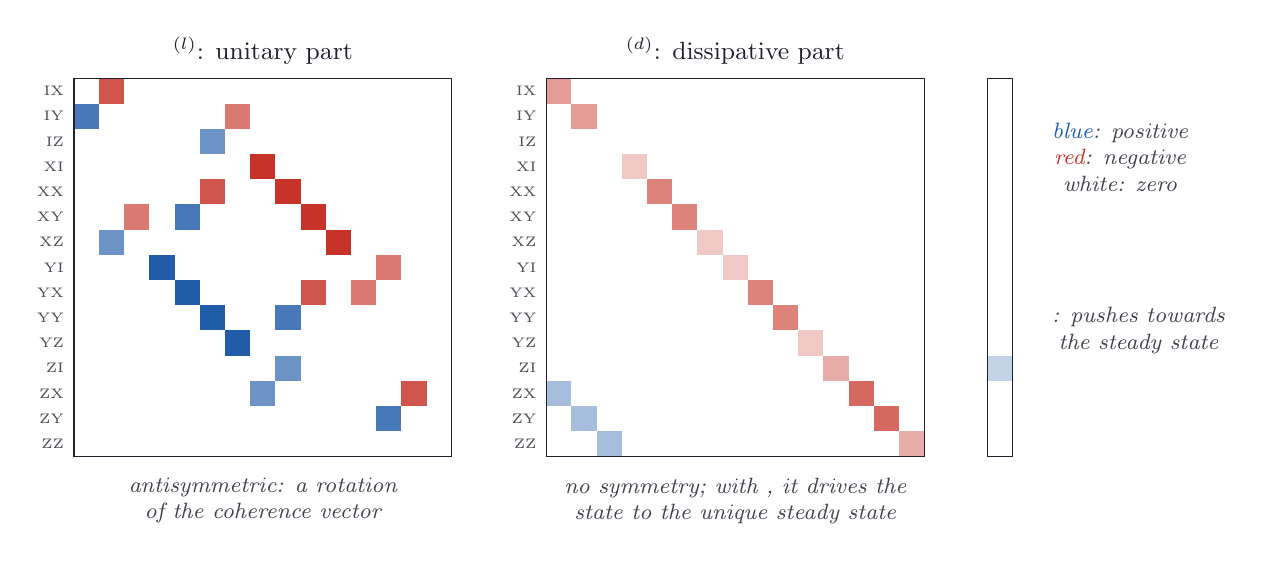
\begin{tikzpicture}[ink/.style={line width=0.9pt, ndInk}, faint/.style={line width=0.4pt, ndInk!35}, dashedink/.style={line width=0.5pt, ndInk!55, dash pattern=on 2.5pt off 2pt}, vec/.style={->, >=stealth, line width=1.2pt}, note/.style={font=\footnotesize\itshape, text=ndInk!85, align=center}, pointer/.style={->, >=stealth, line width=0.4pt, ndInk!60, shorten >=2pt, shorten <=1pt}, dot/.style={circle, fill=ndInk, inner sep=0pt, minimum size=3.4pt}, wash/.style={fill=ndSky, fill opacity=0.55}, every node/.style={text=ndInk}]
\definecolor{ndInk}{rgb}{0.13,0.13,0.18}
\definecolor{ndPaper}{rgb}{0.99,0.96,0.88}
\definecolor{ndSky}{rgb}{0.84,0.91,0.98}
\definecolor{ndRose}{rgb}{0.98,0.86,0.84}
\definecolor{ndBlue}{rgb}{0.13,0.36,0.66}
\definecolor{ndRed}{rgb}{0.78,0.20,0.16}
\definecolor{ndGold}{rgb}{0.88,0.62,0.10}
\definecolor{ndGreen}{rgb}{0.18,0.52,0.30}
\fill[white] (0.000,0.000) rectangle (0.320,-0.320);
\fill[ndRed!83!white] (0.320,0.000) rectangle (0.640,-0.320);
\fill[white] (0.640,0.000) rectangle (0.960,-0.320);
\fill[white] (0.960,0.000) rectangle (1.280,-0.320);
\fill[white] (1.280,0.000) rectangle (1.600,-0.320);
\fill[white] (1.600,0.000) rectangle (1.920,-0.320);
\fill[white] (1.920,0.000) rectangle (2.240,-0.320);
\fill[white] (2.240,0.000) rectangle (2.560,-0.320);
\fill[white] (2.560,0.000) rectangle (2.880,-0.320);
\fill[white] (2.880,0.000) rectangle (3.200,-0.320);
\fill[white] (3.200,0.000) rectangle (3.520,-0.320);
\fill[white] (3.520,0.000) rectangle (3.840,-0.320);
\fill[white] (3.840,0.000) rectangle (4.160,-0.320);
\fill[white] (4.160,0.000) rectangle (4.480,-0.320);
\fill[white] (4.480,0.000) rectangle (4.800,-0.320);
\fill[ndBlue!83!white] (0.000,-0.320) rectangle (0.320,-0.640);
\fill[white] (0.320,-0.320) rectangle (0.640,-0.640);
\fill[white] (0.640,-0.320) rectangle (0.960,-0.640);
\fill[white] (0.960,-0.320) rectangle (1.280,-0.640);
\fill[white] (1.280,-0.320) rectangle (1.600,-0.640);
\fill[white] (1.600,-0.320) rectangle (1.920,-0.640);
\fill[ndRed!66!white] (1.920,-0.320) rectangle (2.240,-0.640);
\fill[white] (2.240,-0.320) rectangle (2.560,-0.640);
\fill[white] (2.560,-0.320) rectangle (2.880,-0.640);
\fill[white] (2.880,-0.320) rectangle (3.200,-0.640);
\fill[white] (3.200,-0.320) rectangle (3.520,-0.640);
\fill[white] (3.520,-0.320) rectangle (3.840,-0.640);
\fill[white] (3.840,-0.320) rectangle (4.160,-0.640);
\fill[white] (4.160,-0.320) rectangle (4.480,-0.640);
\fill[white] (4.480,-0.320) rectangle (4.800,-0.640);
\fill[white] (0.000,-0.640) rectangle (0.320,-0.960);
\fill[white] (0.320,-0.640) rectangle (0.640,-0.960);
\fill[white] (0.640,-0.640) rectangle (0.960,-0.960);
\fill[white] (0.960,-0.640) rectangle (1.280,-0.960);
\fill[white] (1.280,-0.640) rectangle (1.600,-0.960);
\fill[ndBlue!66!white] (1.600,-0.640) rectangle (1.920,-0.960);
\fill[white] (1.920,-0.640) rectangle (2.240,-0.960);
\fill[white] (2.240,-0.640) rectangle (2.560,-0.960);
\fill[white] (2.560,-0.640) rectangle (2.880,-0.960);
\fill[white] (2.880,-0.640) rectangle (3.200,-0.960);
\fill[white] (3.200,-0.640) rectangle (3.520,-0.960);
\fill[white] (3.520,-0.640) rectangle (3.840,-0.960);
\fill[white] (3.840,-0.640) rectangle (4.160,-0.960);
\fill[white] (4.160,-0.640) rectangle (4.480,-0.960);
\fill[white] (4.480,-0.640) rectangle (4.800,-0.960);
\fill[white] (0.000,-0.960) rectangle (0.320,-1.280);
\fill[white] (0.320,-0.960) rectangle (0.640,-1.280);
\fill[white] (0.640,-0.960) rectangle (0.960,-1.280);
\fill[white] (0.960,-0.960) rectangle (1.280,-1.280);
\fill[white] (1.280,-0.960) rectangle (1.600,-1.280);
\fill[white] (1.600,-0.960) rectangle (1.920,-1.280);
\fill[white] (1.920,-0.960) rectangle (2.240,-1.280);
\fill[ndRed!100!white] (2.240,-0.960) rectangle (2.560,-1.280);
\fill[white] (2.560,-0.960) rectangle (2.880,-1.280);
\fill[white] (2.880,-0.960) rectangle (3.200,-1.280);
\fill[white] (3.200,-0.960) rectangle (3.520,-1.280);
\fill[white] (3.520,-0.960) rectangle (3.840,-1.280);
\fill[white] (3.840,-0.960) rectangle (4.160,-1.280);
\fill[white] (4.160,-0.960) rectangle (4.480,-1.280);
\fill[white] (4.480,-0.960) rectangle (4.800,-1.280);
\fill[white] (0.000,-1.280) rectangle (0.320,-1.600);
\fill[white] (0.320,-1.280) rectangle (0.640,-1.600);
\fill[white] (0.640,-1.280) rectangle (0.960,-1.600);
\fill[white] (0.960,-1.280) rectangle (1.280,-1.600);
\fill[white] (1.280,-1.280) rectangle (1.600,-1.600);
\fill[ndRed!83!white] (1.600,-1.280) rectangle (1.920,-1.600);
\fill[white] (1.920,-1.280) rectangle (2.240,-1.600);
\fill[white] (2.240,-1.280) rectangle (2.560,-1.600);
\fill[ndRed!100!white] (2.560,-1.280) rectangle (2.880,-1.600);
\fill[white] (2.880,-1.280) rectangle (3.200,-1.600);
\fill[white] (3.200,-1.280) rectangle (3.520,-1.600);
\fill[white] (3.520,-1.280) rectangle (3.840,-1.600);
\fill[white] (3.840,-1.280) rectangle (4.160,-1.600);
\fill[white] (4.160,-1.280) rectangle (4.480,-1.600);
\fill[white] (4.480,-1.280) rectangle (4.800,-1.600);
\fill[white] (0.000,-1.600) rectangle (0.320,-1.920);
\fill[white] (0.320,-1.600) rectangle (0.640,-1.920);
\fill[ndRed!66!white] (0.640,-1.600) rectangle (0.960,-1.920);
\fill[white] (0.960,-1.600) rectangle (1.280,-1.920);
\fill[ndBlue!83!white] (1.280,-1.600) rectangle (1.600,-1.920);
\fill[white] (1.600,-1.600) rectangle (1.920,-1.920);
\fill[white] (1.920,-1.600) rectangle (2.240,-1.920);
\fill[white] (2.240,-1.600) rectangle (2.560,-1.920);
\fill[white] (2.560,-1.600) rectangle (2.880,-1.920);
\fill[ndRed!100!white] (2.880,-1.600) rectangle (3.200,-1.920);
\fill[white] (3.200,-1.600) rectangle (3.520,-1.920);
\fill[white] (3.520,-1.600) rectangle (3.840,-1.920);
\fill[white] (3.840,-1.600) rectangle (4.160,-1.920);
\fill[white] (4.160,-1.600) rectangle (4.480,-1.920);
\fill[white] (4.480,-1.600) rectangle (4.800,-1.920);
\fill[white] (0.000,-1.920) rectangle (0.320,-2.240);
\fill[ndBlue!66!white] (0.320,-1.920) rectangle (0.640,-2.240);
\fill[white] (0.640,-1.920) rectangle (0.960,-2.240);
\fill[white] (0.960,-1.920) rectangle (1.280,-2.240);
\fill[white] (1.280,-1.920) rectangle (1.600,-2.240);
\fill[white] (1.600,-1.920) rectangle (1.920,-2.240);
\fill[white] (1.920,-1.920) rectangle (2.240,-2.240);
\fill[white] (2.240,-1.920) rectangle (2.560,-2.240);
\fill[white] (2.560,-1.920) rectangle (2.880,-2.240);
\fill[white] (2.880,-1.920) rectangle (3.200,-2.240);
\fill[ndRed!100!white] (3.200,-1.920) rectangle (3.520,-2.240);
\fill[white] (3.520,-1.920) rectangle (3.840,-2.240);
\fill[white] (3.840,-1.920) rectangle (4.160,-2.240);
\fill[white] (4.160,-1.920) rectangle (4.480,-2.240);
\fill[white] (4.480,-1.920) rectangle (4.800,-2.240);
\fill[white] (0.000,-2.240) rectangle (0.320,-2.560);
\fill[white] (0.320,-2.240) rectangle (0.640,-2.560);
\fill[white] (0.640,-2.240) rectangle (0.960,-2.560);
\fill[ndBlue!100!white] (0.960,-2.240) rectangle (1.280,-2.560);
\fill[white] (1.280,-2.240) rectangle (1.600,-2.560);
\fill[white] (1.600,-2.240) rectangle (1.920,-2.560);
\fill[white] (1.920,-2.240) rectangle (2.240,-2.560);
\fill[white] (2.240,-2.240) rectangle (2.560,-2.560);
\fill[white] (2.560,-2.240) rectangle (2.880,-2.560);
\fill[white] (2.880,-2.240) rectangle (3.200,-2.560);
\fill[white] (3.200,-2.240) rectangle (3.520,-2.560);
\fill[white] (3.520,-2.240) rectangle (3.840,-2.560);
\fill[ndRed!66!white] (3.840,-2.240) rectangle (4.160,-2.560);
\fill[white] (4.160,-2.240) rectangle (4.480,-2.560);
\fill[white] (4.480,-2.240) rectangle (4.800,-2.560);
\fill[white] (0.000,-2.560) rectangle (0.320,-2.880);
\fill[white] (0.320,-2.560) rectangle (0.640,-2.880);
\fill[white] (0.640,-2.560) rectangle (0.960,-2.880);
\fill[white] (0.960,-2.560) rectangle (1.280,-2.880);
\fill[ndBlue!100!white] (1.280,-2.560) rectangle (1.600,-2.880);
\fill[white] (1.600,-2.560) rectangle (1.920,-2.880);
\fill[white] (1.920,-2.560) rectangle (2.240,-2.880);
\fill[white] (2.240,-2.560) rectangle (2.560,-2.880);
\fill[white] (2.560,-2.560) rectangle (2.880,-2.880);
\fill[ndRed!83!white] (2.880,-2.560) rectangle (3.200,-2.880);
\fill[white] (3.200,-2.560) rectangle (3.520,-2.880);
\fill[ndRed!66!white] (3.520,-2.560) rectangle (3.840,-2.880);
\fill[white] (3.840,-2.560) rectangle (4.160,-2.880);
\fill[white] (4.160,-2.560) rectangle (4.480,-2.880);
\fill[white] (4.480,-2.560) rectangle (4.800,-2.880);
\fill[white] (0.000,-2.880) rectangle (0.320,-3.200);
\fill[white] (0.320,-2.880) rectangle (0.640,-3.200);
\fill[white] (0.640,-2.880) rectangle (0.960,-3.200);
\fill[white] (0.960,-2.880) rectangle (1.280,-3.200);
\fill[white] (1.280,-2.880) rectangle (1.600,-3.200);
\fill[ndBlue!100!white] (1.600,-2.880) rectangle (1.920,-3.200);
\fill[white] (1.920,-2.880) rectangle (2.240,-3.200);
\fill[white] (2.240,-2.880) rectangle (2.560,-3.200);
\fill[ndBlue!83!white] (2.560,-2.880) rectangle (2.880,-3.200);
\fill[white] (2.880,-2.880) rectangle (3.200,-3.200);
\fill[white] (3.200,-2.880) rectangle (3.520,-3.200);
\fill[white] (3.520,-2.880) rectangle (3.840,-3.200);
\fill[white] (3.840,-2.880) rectangle (4.160,-3.200);
\fill[white] (4.160,-2.880) rectangle (4.480,-3.200);
\fill[white] (4.480,-2.880) rectangle (4.800,-3.200);
\fill[white] (0.000,-3.200) rectangle (0.320,-3.520);
\fill[white] (0.320,-3.200) rectangle (0.640,-3.520);
\fill[white] (0.640,-3.200) rectangle (0.960,-3.520);
\fill[white] (0.960,-3.200) rectangle (1.280,-3.520);
\fill[white] (1.280,-3.200) rectangle (1.600,-3.520);
\fill[white] (1.600,-3.200) rectangle (1.920,-3.520);
\fill[ndBlue!100!white] (1.920,-3.200) rectangle (2.240,-3.520);
\fill[white] (2.240,-3.200) rectangle (2.560,-3.520);
\fill[white] (2.560,-3.200) rectangle (2.880,-3.520);
\fill[white] (2.880,-3.200) rectangle (3.200,-3.520);
\fill[white] (3.200,-3.200) rectangle (3.520,-3.520);
\fill[white] (3.520,-3.200) rectangle (3.840,-3.520);
\fill[white] (3.840,-3.200) rectangle (4.160,-3.520);
\fill[white] (4.160,-3.200) rectangle (4.480,-3.520);
\fill[white] (4.480,-3.200) rectangle (4.800,-3.520);
\fill[white] (0.000,-3.520) rectangle (0.320,-3.840);
\fill[white] (0.320,-3.520) rectangle (0.640,-3.840);
\fill[white] (0.640,-3.520) rectangle (0.960,-3.840);
\fill[white] (0.960,-3.520) rectangle (1.280,-3.840);
\fill[white] (1.280,-3.520) rectangle (1.600,-3.840);
\fill[white] (1.600,-3.520) rectangle (1.920,-3.840);
\fill[white] (1.920,-3.520) rectangle (2.240,-3.840);
\fill[white] (2.240,-3.520) rectangle (2.560,-3.840);
\fill[ndBlue!66!white] (2.560,-3.520) rectangle (2.880,-3.840);
\fill[white] (2.880,-3.520) rectangle (3.200,-3.840);
\fill[white] (3.200,-3.520) rectangle (3.520,-3.840);
\fill[white] (3.520,-3.520) rectangle (3.840,-3.840);
\fill[white] (3.840,-3.520) rectangle (4.160,-3.840);
\fill[white] (4.160,-3.520) rectangle (4.480,-3.840);
\fill[white] (4.480,-3.520) rectangle (4.800,-3.840);
\fill[white] (0.000,-3.840) rectangle (0.320,-4.160);
\fill[white] (0.320,-3.840) rectangle (0.640,-4.160);
\fill[white] (0.640,-3.840) rectangle (0.960,-4.160);
\fill[white] (0.960,-3.840) rectangle (1.280,-4.160);
\fill[white] (1.280,-3.840) rectangle (1.600,-4.160);
\fill[white] (1.600,-3.840) rectangle (1.920,-4.160);
\fill[white] (1.920,-3.840) rectangle (2.240,-4.160);
\fill[ndBlue!66!white] (2.240,-3.840) rectangle (2.560,-4.160);
\fill[white] (2.560,-3.840) rectangle (2.880,-4.160);
\fill[white] (2.880,-3.840) rectangle (3.200,-4.160);
\fill[white] (3.200,-3.840) rectangle (3.520,-4.160);
\fill[white] (3.520,-3.840) rectangle (3.840,-4.160);
\fill[white] (3.840,-3.840) rectangle (4.160,-4.160);
\fill[ndRed!83!white] (4.160,-3.840) rectangle (4.480,-4.160);
\fill[white] (4.480,-3.840) rectangle (4.800,-4.160);
\fill[white] (0.000,-4.160) rectangle (0.320,-4.480);
\fill[white] (0.320,-4.160) rectangle (0.640,-4.480);
\fill[white] (0.640,-4.160) rectangle (0.960,-4.480);
\fill[white] (0.960,-4.160) rectangle (1.280,-4.480);
\fill[white] (1.280,-4.160) rectangle (1.600,-4.480);
\fill[white] (1.600,-4.160) rectangle (1.920,-4.480);
\fill[white] (1.920,-4.160) rectangle (2.240,-4.480);
\fill[white] (2.240,-4.160) rectangle (2.560,-4.480);
\fill[white] (2.560,-4.160) rectangle (2.880,-4.480);
\fill[white] (2.880,-4.160) rectangle (3.200,-4.480);
\fill[white] (3.200,-4.160) rectangle (3.520,-4.480);
\fill[white] (3.520,-4.160) rectangle (3.840,-4.480);
\fill[ndBlue!83!white] (3.840,-4.160) rectangle (4.160,-4.480);
\fill[white] (4.160,-4.160) rectangle (4.480,-4.480);
\fill[white] (4.480,-4.160) rectangle (4.800,-4.480);
\fill[white] (0.000,-4.480) rectangle (0.320,-4.800);
\fill[white] (0.320,-4.480) rectangle (0.640,-4.800);
\fill[white] (0.640,-4.480) rectangle (0.960,-4.800);
\fill[white] (0.960,-4.480) rectangle (1.280,-4.800);
\fill[white] (1.280,-4.480) rectangle (1.600,-4.800);
\fill[white] (1.600,-4.480) rectangle (1.920,-4.800);
\fill[white] (1.920,-4.480) rectangle (2.240,-4.800);
\fill[white] (2.240,-4.480) rectangle (2.560,-4.800);
\fill[white] (2.560,-4.480) rectangle (2.880,-4.800);
\fill[white] (2.880,-4.480) rectangle (3.200,-4.800);
\fill[white] (3.200,-4.480) rectangle (3.520,-4.800);
\fill[white] (3.520,-4.480) rectangle (3.840,-4.800);
\fill[white] (3.840,-4.480) rectangle (4.160,-4.800);
\fill[white] (4.160,-4.480) rectangle (4.480,-4.800);
\fill[white] (4.480,-4.480) rectangle (4.800,-4.800);
\draw[ink, line width=0.5pt] (0.000,0.000) rectangle (4.800,-4.800);
\node[font=\tiny, left, text=ndInk!80] at (0.000,-0.160) {IX};
\node[font=\tiny, left, text=ndInk!80] at (0.000,-0.480) {IY};
\node[font=\tiny, left, text=ndInk!80] at (0.000,-0.800) {IZ};
\node[font=\tiny, left, text=ndInk!80] at (0.000,-1.120) {XI};
\node[font=\tiny, left, text=ndInk!80] at (0.000,-1.440) {XX};
\node[font=\tiny, left, text=ndInk!80] at (0.000,-1.760) {XY};
\node[font=\tiny, left, text=ndInk!80] at (0.000,-2.080) {XZ};
\node[font=\tiny, left, text=ndInk!80] at (0.000,-2.400) {YI};
\node[font=\tiny, left, text=ndInk!80] at (0.000,-2.720) {YX};
\node[font=\tiny, left, text=ndInk!80] at (0.000,-3.040) {YY};
\node[font=\tiny, left, text=ndInk!80] at (0.000,-3.360) {YZ};
\node[font=\tiny, left, text=ndInk!80] at (0.000,-3.680) {ZI};
\node[font=\tiny, left, text=ndInk!80] at (0.000,-4.000) {ZX};
\node[font=\tiny, left, text=ndInk!80] at (0.000,-4.320) {ZY};
\node[font=\tiny, left, text=ndInk!80] at (0.000,-4.640) {ZZ};
\node[font=\small, above] at (2.400,0.050) {$\Amat^{(l)}$: unitary part};
\fill[ndRed!49!white] (6.000,0.000) rectangle (6.320,-0.320);
\fill[white] (6.320,0.000) rectangle (6.640,-0.320);
\fill[white] (6.640,0.000) rectangle (6.960,-0.320);
\fill[white] (6.960,0.000) rectangle (7.280,-0.320);
\fill[white] (7.280,0.000) rectangle (7.600,-0.320);
\fill[white] (7.600,0.000) rectangle (7.920,-0.320);
\fill[white] (7.920,0.000) rectangle (8.240,-0.320);
\fill[white] (8.240,0.000) rectangle (8.560,-0.320);
\fill[white] (8.560,0.000) rectangle (8.880,-0.320);
\fill[white] (8.880,0.000) rectangle (9.200,-0.320);
\fill[white] (9.200,0.000) rectangle (9.520,-0.320);
\fill[white] (9.520,0.000) rectangle (9.840,-0.320);
\fill[white] (9.840,0.000) rectangle (10.160,-0.320);
\fill[white] (10.160,0.000) rectangle (10.480,-0.320);
\fill[white] (10.480,0.000) rectangle (10.800,-0.320);
\fill[white] (6.000,-0.320) rectangle (6.320,-0.640);
\fill[ndRed!49!white] (6.320,-0.320) rectangle (6.640,-0.640);
\fill[white] (6.640,-0.320) rectangle (6.960,-0.640);
\fill[white] (6.960,-0.320) rectangle (7.280,-0.640);
\fill[white] (7.280,-0.320) rectangle (7.600,-0.640);
\fill[white] (7.600,-0.320) rectangle (7.920,-0.640);
\fill[white] (7.920,-0.320) rectangle (8.240,-0.640);
\fill[white] (8.240,-0.320) rectangle (8.560,-0.640);
\fill[white] (8.560,-0.320) rectangle (8.880,-0.640);
\fill[white] (8.880,-0.320) rectangle (9.200,-0.640);
\fill[white] (9.200,-0.320) rectangle (9.520,-0.640);
\fill[white] (9.520,-0.320) rectangle (9.840,-0.640);
\fill[white] (9.840,-0.320) rectangle (10.160,-0.640);
\fill[white] (10.160,-0.320) rectangle (10.480,-0.640);
\fill[white] (10.480,-0.320) rectangle (10.800,-0.640);
\fill[white] (6.000,-0.640) rectangle (6.320,-0.960);
\fill[white] (6.320,-0.640) rectangle (6.640,-0.960);
\fill[white] (6.640,-0.640) rectangle (6.960,-0.960);
\fill[white] (6.960,-0.640) rectangle (7.280,-0.960);
\fill[white] (7.280,-0.640) rectangle (7.600,-0.960);
\fill[white] (7.600,-0.640) rectangle (7.920,-0.960);
\fill[white] (7.920,-0.640) rectangle (8.240,-0.960);
\fill[white] (8.240,-0.640) rectangle (8.560,-0.960);
\fill[white] (8.560,-0.640) rectangle (8.880,-0.960);
\fill[white] (8.880,-0.640) rectangle (9.200,-0.960);
\fill[white] (9.200,-0.640) rectangle (9.520,-0.960);
\fill[white] (9.520,-0.640) rectangle (9.840,-0.960);
\fill[white] (9.840,-0.640) rectangle (10.160,-0.960);
\fill[white] (10.160,-0.640) rectangle (10.480,-0.960);
\fill[white] (10.480,-0.640) rectangle (10.800,-0.960);
\fill[white] (6.000,-0.960) rectangle (6.320,-1.280);
\fill[white] (6.320,-0.960) rectangle (6.640,-1.280);
\fill[white] (6.640,-0.960) rectangle (6.960,-1.280);
\fill[ndRed!27!white] (6.960,-0.960) rectangle (7.280,-1.280);
\fill[white] (7.280,-0.960) rectangle (7.600,-1.280);
\fill[white] (7.600,-0.960) rectangle (7.920,-1.280);
\fill[white] (7.920,-0.960) rectangle (8.240,-1.280);
\fill[white] (8.240,-0.960) rectangle (8.560,-1.280);
\fill[white] (8.560,-0.960) rectangle (8.880,-1.280);
\fill[white] (8.880,-0.960) rectangle (9.200,-1.280);
\fill[white] (9.200,-0.960) rectangle (9.520,-1.280);
\fill[white] (9.520,-0.960) rectangle (9.840,-1.280);
\fill[white] (9.840,-0.960) rectangle (10.160,-1.280);
\fill[white] (10.160,-0.960) rectangle (10.480,-1.280);
\fill[white] (10.480,-0.960) rectangle (10.800,-1.280);
\fill[white] (6.000,-1.280) rectangle (6.320,-1.600);
\fill[white] (6.320,-1.280) rectangle (6.640,-1.600);
\fill[white] (6.640,-1.280) rectangle (6.960,-1.600);
\fill[white] (6.960,-1.280) rectangle (7.280,-1.600);
\fill[ndRed!61!white] (7.280,-1.280) rectangle (7.600,-1.600);
\fill[white] (7.600,-1.280) rectangle (7.920,-1.600);
\fill[white] (7.920,-1.280) rectangle (8.240,-1.600);
\fill[white] (8.240,-1.280) rectangle (8.560,-1.600);
\fill[white] (8.560,-1.280) rectangle (8.880,-1.600);
\fill[white] (8.880,-1.280) rectangle (9.200,-1.600);
\fill[white] (9.200,-1.280) rectangle (9.520,-1.600);
\fill[white] (9.520,-1.280) rectangle (9.840,-1.600);
\fill[white] (9.840,-1.280) rectangle (10.160,-1.600);
\fill[white] (10.160,-1.280) rectangle (10.480,-1.600);
\fill[white] (10.480,-1.280) rectangle (10.800,-1.600);
\fill[white] (6.000,-1.600) rectangle (6.320,-1.920);
\fill[white] (6.320,-1.600) rectangle (6.640,-1.920);
\fill[white] (6.640,-1.600) rectangle (6.960,-1.920);
\fill[white] (6.960,-1.600) rectangle (7.280,-1.920);
\fill[white] (7.280,-1.600) rectangle (7.600,-1.920);
\fill[ndRed!61!white] (7.600,-1.600) rectangle (7.920,-1.920);
\fill[white] (7.920,-1.600) rectangle (8.240,-1.920);
\fill[white] (8.240,-1.600) rectangle (8.560,-1.920);
\fill[white] (8.560,-1.600) rectangle (8.880,-1.920);
\fill[white] (8.880,-1.600) rectangle (9.200,-1.920);
\fill[white] (9.200,-1.600) rectangle (9.520,-1.920);
\fill[white] (9.520,-1.600) rectangle (9.840,-1.920);
\fill[white] (9.840,-1.600) rectangle (10.160,-1.920);
\fill[white] (10.160,-1.600) rectangle (10.480,-1.920);
\fill[white] (10.480,-1.600) rectangle (10.800,-1.920);
\fill[white] (6.000,-1.920) rectangle (6.320,-2.240);
\fill[white] (6.320,-1.920) rectangle (6.640,-2.240);
\fill[white] (6.640,-1.920) rectangle (6.960,-2.240);
\fill[white] (6.960,-1.920) rectangle (7.280,-2.240);
\fill[white] (7.280,-1.920) rectangle (7.600,-2.240);
\fill[white] (7.600,-1.920) rectangle (7.920,-2.240);
\fill[ndRed!27!white] (7.920,-1.920) rectangle (8.240,-2.240);
\fill[white] (8.240,-1.920) rectangle (8.560,-2.240);
\fill[white] (8.560,-1.920) rectangle (8.880,-2.240);
\fill[white] (8.880,-1.920) rectangle (9.200,-2.240);
\fill[white] (9.200,-1.920) rectangle (9.520,-2.240);
\fill[white] (9.520,-1.920) rectangle (9.840,-2.240);
\fill[white] (9.840,-1.920) rectangle (10.160,-2.240);
\fill[white] (10.160,-1.920) rectangle (10.480,-2.240);
\fill[white] (10.480,-1.920) rectangle (10.800,-2.240);
\fill[white] (6.000,-2.240) rectangle (6.320,-2.560);
\fill[white] (6.320,-2.240) rectangle (6.640,-2.560);
\fill[white] (6.640,-2.240) rectangle (6.960,-2.560);
\fill[white] (6.960,-2.240) rectangle (7.280,-2.560);
\fill[white] (7.280,-2.240) rectangle (7.600,-2.560);
\fill[white] (7.600,-2.240) rectangle (7.920,-2.560);
\fill[white] (7.920,-2.240) rectangle (8.240,-2.560);
\fill[ndRed!27!white] (8.240,-2.240) rectangle (8.560,-2.560);
\fill[white] (8.560,-2.240) rectangle (8.880,-2.560);
\fill[white] (8.880,-2.240) rectangle (9.200,-2.560);
\fill[white] (9.200,-2.240) rectangle (9.520,-2.560);
\fill[white] (9.520,-2.240) rectangle (9.840,-2.560);
\fill[white] (9.840,-2.240) rectangle (10.160,-2.560);
\fill[white] (10.160,-2.240) rectangle (10.480,-2.560);
\fill[white] (10.480,-2.240) rectangle (10.800,-2.560);
\fill[white] (6.000,-2.560) rectangle (6.320,-2.880);
\fill[white] (6.320,-2.560) rectangle (6.640,-2.880);
\fill[white] (6.640,-2.560) rectangle (6.960,-2.880);
\fill[white] (6.960,-2.560) rectangle (7.280,-2.880);
\fill[white] (7.280,-2.560) rectangle (7.600,-2.880);
\fill[white] (7.600,-2.560) rectangle (7.920,-2.880);
\fill[white] (7.920,-2.560) rectangle (8.240,-2.880);
\fill[white] (8.240,-2.560) rectangle (8.560,-2.880);
\fill[ndRed!61!white] (8.560,-2.560) rectangle (8.880,-2.880);
\fill[white] (8.880,-2.560) rectangle (9.200,-2.880);
\fill[white] (9.200,-2.560) rectangle (9.520,-2.880);
\fill[white] (9.520,-2.560) rectangle (9.840,-2.880);
\fill[white] (9.840,-2.560) rectangle (10.160,-2.880);
\fill[white] (10.160,-2.560) rectangle (10.480,-2.880);
\fill[white] (10.480,-2.560) rectangle (10.800,-2.880);
\fill[white] (6.000,-2.880) rectangle (6.320,-3.200);
\fill[white] (6.320,-2.880) rectangle (6.640,-3.200);
\fill[white] (6.640,-2.880) rectangle (6.960,-3.200);
\fill[white] (6.960,-2.880) rectangle (7.280,-3.200);
\fill[white] (7.280,-2.880) rectangle (7.600,-3.200);
\fill[white] (7.600,-2.880) rectangle (7.920,-3.200);
\fill[white] (7.920,-2.880) rectangle (8.240,-3.200);
\fill[white] (8.240,-2.880) rectangle (8.560,-3.200);
\fill[white] (8.560,-2.880) rectangle (8.880,-3.200);
\fill[ndRed!61!white] (8.880,-2.880) rectangle (9.200,-3.200);
\fill[white] (9.200,-2.880) rectangle (9.520,-3.200);
\fill[white] (9.520,-2.880) rectangle (9.840,-3.200);
\fill[white] (9.840,-2.880) rectangle (10.160,-3.200);
\fill[white] (10.160,-2.880) rectangle (10.480,-3.200);
\fill[white] (10.480,-2.880) rectangle (10.800,-3.200);
\fill[white] (6.000,-3.200) rectangle (6.320,-3.520);
\fill[white] (6.320,-3.200) rectangle (6.640,-3.520);
\fill[white] (6.640,-3.200) rectangle (6.960,-3.520);
\fill[white] (6.960,-3.200) rectangle (7.280,-3.520);
\fill[white] (7.280,-3.200) rectangle (7.600,-3.520);
\fill[white] (7.600,-3.200) rectangle (7.920,-3.520);
\fill[white] (7.920,-3.200) rectangle (8.240,-3.520);
\fill[white] (8.240,-3.200) rectangle (8.560,-3.520);
\fill[white] (8.560,-3.200) rectangle (8.880,-3.520);
\fill[white] (8.880,-3.200) rectangle (9.200,-3.520);
\fill[ndRed!27!white] (9.200,-3.200) rectangle (9.520,-3.520);
\fill[white] (9.520,-3.200) rectangle (9.840,-3.520);
\fill[white] (9.840,-3.200) rectangle (10.160,-3.520);
\fill[white] (10.160,-3.200) rectangle (10.480,-3.520);
\fill[white] (10.480,-3.200) rectangle (10.800,-3.520);
\fill[white] (6.000,-3.520) rectangle (6.320,-3.840);
\fill[white] (6.320,-3.520) rectangle (6.640,-3.840);
\fill[white] (6.640,-3.520) rectangle (6.960,-3.840);
\fill[white] (6.960,-3.520) rectangle (7.280,-3.840);
\fill[white] (7.280,-3.520) rectangle (7.600,-3.840);
\fill[white] (7.600,-3.520) rectangle (7.920,-3.840);
\fill[white] (7.920,-3.520) rectangle (8.240,-3.840);
\fill[white] (8.240,-3.520) rectangle (8.560,-3.840);
\fill[white] (8.560,-3.520) rectangle (8.880,-3.840);
\fill[white] (8.880,-3.520) rectangle (9.200,-3.840);
\fill[white] (9.200,-3.520) rectangle (9.520,-3.840);
\fill[ndRed!40!white] (9.520,-3.520) rectangle (9.840,-3.840);
\fill[white] (9.840,-3.520) rectangle (10.160,-3.840);
\fill[white] (10.160,-3.520) rectangle (10.480,-3.840);
\fill[white] (10.480,-3.520) rectangle (10.800,-3.840);
\fill[ndBlue!40!white] (6.000,-3.840) rectangle (6.320,-4.160);
\fill[white] (6.320,-3.840) rectangle (6.640,-4.160);
\fill[white] (6.640,-3.840) rectangle (6.960,-4.160);
\fill[white] (6.960,-3.840) rectangle (7.280,-4.160);
\fill[white] (7.280,-3.840) rectangle (7.600,-4.160);
\fill[white] (7.600,-3.840) rectangle (7.920,-4.160);
\fill[white] (7.920,-3.840) rectangle (8.240,-4.160);
\fill[white] (8.240,-3.840) rectangle (8.560,-4.160);
\fill[white] (8.560,-3.840) rectangle (8.880,-4.160);
\fill[white] (8.880,-3.840) rectangle (9.200,-4.160);
\fill[white] (9.200,-3.840) rectangle (9.520,-4.160);
\fill[white] (9.520,-3.840) rectangle (9.840,-4.160);
\fill[ndRed!74!white] (9.840,-3.840) rectangle (10.160,-4.160);
\fill[white] (10.160,-3.840) rectangle (10.480,-4.160);
\fill[white] (10.480,-3.840) rectangle (10.800,-4.160);
\fill[white] (6.000,-4.160) rectangle (6.320,-4.480);
\fill[ndBlue!40!white] (6.320,-4.160) rectangle (6.640,-4.480);
\fill[white] (6.640,-4.160) rectangle (6.960,-4.480);
\fill[white] (6.960,-4.160) rectangle (7.280,-4.480);
\fill[white] (7.280,-4.160) rectangle (7.600,-4.480);
\fill[white] (7.600,-4.160) rectangle (7.920,-4.480);
\fill[white] (7.920,-4.160) rectangle (8.240,-4.480);
\fill[white] (8.240,-4.160) rectangle (8.560,-4.480);
\fill[white] (8.560,-4.160) rectangle (8.880,-4.480);
\fill[white] (8.880,-4.160) rectangle (9.200,-4.480);
\fill[white] (9.200,-4.160) rectangle (9.520,-4.480);
\fill[white] (9.520,-4.160) rectangle (9.840,-4.480);
\fill[white] (9.840,-4.160) rectangle (10.160,-4.480);
\fill[ndRed!74!white] (10.160,-4.160) rectangle (10.480,-4.480);
\fill[white] (10.480,-4.160) rectangle (10.800,-4.480);
\fill[white] (6.000,-4.480) rectangle (6.320,-4.800);
\fill[white] (6.320,-4.480) rectangle (6.640,-4.800);
\fill[ndBlue!40!white] (6.640,-4.480) rectangle (6.960,-4.800);
\fill[white] (6.960,-4.480) rectangle (7.280,-4.800);
\fill[white] (7.280,-4.480) rectangle (7.600,-4.800);
\fill[white] (7.600,-4.480) rectangle (7.920,-4.800);
\fill[white] (7.920,-4.480) rectangle (8.240,-4.800);
\fill[white] (8.240,-4.480) rectangle (8.560,-4.800);
\fill[white] (8.560,-4.480) rectangle (8.880,-4.800);
\fill[white] (8.880,-4.480) rectangle (9.200,-4.800);
\fill[white] (9.200,-4.480) rectangle (9.520,-4.800);
\fill[white] (9.520,-4.480) rectangle (9.840,-4.800);
\fill[white] (9.840,-4.480) rectangle (10.160,-4.800);
\fill[white] (10.160,-4.480) rectangle (10.480,-4.800);
\fill[ndRed!40!white] (10.480,-4.480) rectangle (10.800,-4.800);
\draw[ink, line width=0.5pt] (6.000,0.000) rectangle (10.800,-4.800);
\node[font=\tiny, left, text=ndInk!80] at (6.000,-0.160) {IX};
\node[font=\tiny, left, text=ndInk!80] at (6.000,-0.480) {IY};
\node[font=\tiny, left, text=ndInk!80] at (6.000,-0.800) {IZ};
\node[font=\tiny, left, text=ndInk!80] at (6.000,-1.120) {XI};
\node[font=\tiny, left, text=ndInk!80] at (6.000,-1.440) {XX};
\node[font=\tiny, left, text=ndInk!80] at (6.000,-1.760) {XY};
\node[font=\tiny, left, text=ndInk!80] at (6.000,-2.080) {XZ};
\node[font=\tiny, left, text=ndInk!80] at (6.000,-2.400) {YI};
\node[font=\tiny, left, text=ndInk!80] at (6.000,-2.720) {YX};
\node[font=\tiny, left, text=ndInk!80] at (6.000,-3.040) {YY};
\node[font=\tiny, left, text=ndInk!80] at (6.000,-3.360) {YZ};
\node[font=\tiny, left, text=ndInk!80] at (6.000,-3.680) {ZI};
\node[font=\tiny, left, text=ndInk!80] at (6.000,-4.000) {ZX};
\node[font=\tiny, left, text=ndInk!80] at (6.000,-4.320) {ZY};
\node[font=\tiny, left, text=ndInk!80] at (6.000,-4.640) {ZZ};
\node[font=\small, above] at (8.400,0.050) {$\Amat^{(d)}$: dissipative part};
\fill[white] (11.600,0.000) rectangle (11.920,-0.320);
\fill[white] (11.600,-0.320) rectangle (11.920,-0.640);
\fill[white] (11.600,-0.640) rectangle (11.920,-0.960);
\fill[white] (11.600,-0.960) rectangle (11.920,-1.280);
\fill[white] (11.600,-1.280) rectangle (11.920,-1.600);
\fill[white] (11.600,-1.600) rectangle (11.920,-1.920);
\fill[white] (11.600,-1.920) rectangle (11.920,-2.240);
\fill[white] (11.600,-2.240) rectangle (11.920,-2.560);
\fill[white] (11.600,-2.560) rectangle (11.920,-2.880);
\fill[white] (11.600,-2.880) rectangle (11.920,-3.200);
\fill[white] (11.600,-3.200) rectangle (11.920,-3.520);
\fill[ndBlue!27!white] (11.600,-3.520) rectangle (11.920,-3.840);
\fill[white] (11.600,-3.840) rectangle (11.920,-4.160);
\fill[white] (11.600,-4.160) rectangle (11.920,-4.480);
\fill[white] (11.600,-4.480) rectangle (11.920,-4.800);
\draw[ink, line width=0.5pt] (11.600,0.000) rectangle (11.920,-4.800);
\node[font=\small, above] at (11.760,0.050) {$\bvec$};
\node[note, anchor=north] at (2.4,-4.95) {antisymmetric: a rotation\\ of the coherence vector};
\node[note, anchor=north] at (8.4,-4.95) {no symmetry; with $\bvec$, it drives the\\ state to the unique steady state};
\node[note, anchor=west] at (12.3,-3.2) {$\bvec$: pushes towards\\ the steady state};
\node[note, anchor=west] at (12.3,-1.0) {\textcolor{ndBlue}{blue}: positive\\ \textcolor{ndRed}{red}: negative\\ white: zero};
\end{tikzpicture}
}
\caption{The matrices $\Amat^{(l)}$, $\Amat^{(d)}$ and the vector $\bvec$ for a two-qubit model in the normalised Pauli basis (rows labelled by Pauli strings); blue entries are positive, red negative, white zero. Generated by \texttt{code/ch03\_amatrix.py}.}\label{fig:ch03:amatrix}
\end{figure}}
\ona{\endgraf\medskip\noindent\textit{Reading the figure.} Each small square is one entry of a $15\times15$ matrix, and each row and column is labelled by a two-qubit observable (a Pauli string). Blue entries are positive, red negative, white zero, and darker means larger in magnitude. The left matrix comes from the Hamiltonian, the middle one from the noise, and the single column on the right is the constant term $\bvec$.\endgraf\smallskip\noindent\textit{Why it matters.} This is the quantum system written as a classical state-space model $\dot{\vec x}=\Amat\vec x+\bvec$, to which every tool of linear systems applies, whether one learnt it in a control, signal-processing or numerical-analysis course. The left matrix is antisymmetric: it describes reversible motion, which preserves the length of $\vec x$ (the purity). The middle one describes irreversible effects. Most entries are zero, and the non-zero ones depend on only a handful of physical parameters, five here, against $225$ entries. This sparsity is why identification is feasible at all.}
\onp{\begin{center}\resizebox{\linewidth}{!}{% Generated by code/needham.py -- do not edit by hand.
\definecolor{qocA}{rgb}{0.00,0.45,0.70}
\definecolor{qocB}{rgb}{0.90,0.60,0.00}
\definecolor{qocC}{rgb}{0.00,0.62,0.45}
\definecolor{qocD}{rgb}{0.80,0.40,0.00}
\definecolor{qocE}{rgb}{0.80,0.60,0.70}
\definecolor{qocF}{rgb}{0.35,0.70,0.90}
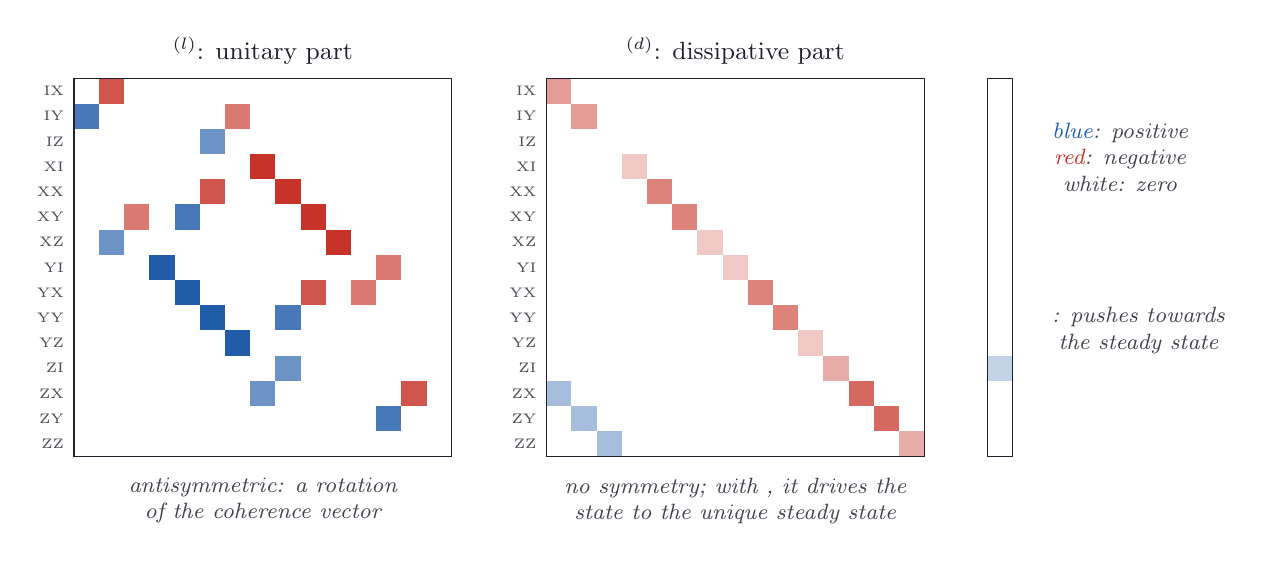
\begin{tikzpicture}[ink/.style={line width=0.9pt, ndInk}, faint/.style={line width=0.4pt, ndInk!35}, dashedink/.style={line width=0.5pt, ndInk!55, dash pattern=on 2.5pt off 2pt}, vec/.style={->, >=stealth, line width=1.2pt}, note/.style={font=\footnotesize\itshape, text=ndInk!85, align=center}, pointer/.style={->, >=stealth, line width=0.4pt, ndInk!60, shorten >=2pt, shorten <=1pt}, dot/.style={circle, fill=ndInk, inner sep=0pt, minimum size=3.4pt}, wash/.style={fill=ndSky, fill opacity=0.55}, every node/.style={text=ndInk}]
\definecolor{ndInk}{rgb}{0.13,0.13,0.18}
\definecolor{ndPaper}{rgb}{0.99,0.96,0.88}
\definecolor{ndSky}{rgb}{0.84,0.91,0.98}
\definecolor{ndRose}{rgb}{0.98,0.86,0.84}
\definecolor{ndBlue}{rgb}{0.13,0.36,0.66}
\definecolor{ndRed}{rgb}{0.78,0.20,0.16}
\definecolor{ndGold}{rgb}{0.88,0.62,0.10}
\definecolor{ndGreen}{rgb}{0.18,0.52,0.30}
\fill[white] (0.000,0.000) rectangle (0.320,-0.320);
\fill[ndRed!83!white] (0.320,0.000) rectangle (0.640,-0.320);
\fill[white] (0.640,0.000) rectangle (0.960,-0.320);
\fill[white] (0.960,0.000) rectangle (1.280,-0.320);
\fill[white] (1.280,0.000) rectangle (1.600,-0.320);
\fill[white] (1.600,0.000) rectangle (1.920,-0.320);
\fill[white] (1.920,0.000) rectangle (2.240,-0.320);
\fill[white] (2.240,0.000) rectangle (2.560,-0.320);
\fill[white] (2.560,0.000) rectangle (2.880,-0.320);
\fill[white] (2.880,0.000) rectangle (3.200,-0.320);
\fill[white] (3.200,0.000) rectangle (3.520,-0.320);
\fill[white] (3.520,0.000) rectangle (3.840,-0.320);
\fill[white] (3.840,0.000) rectangle (4.160,-0.320);
\fill[white] (4.160,0.000) rectangle (4.480,-0.320);
\fill[white] (4.480,0.000) rectangle (4.800,-0.320);
\fill[ndBlue!83!white] (0.000,-0.320) rectangle (0.320,-0.640);
\fill[white] (0.320,-0.320) rectangle (0.640,-0.640);
\fill[white] (0.640,-0.320) rectangle (0.960,-0.640);
\fill[white] (0.960,-0.320) rectangle (1.280,-0.640);
\fill[white] (1.280,-0.320) rectangle (1.600,-0.640);
\fill[white] (1.600,-0.320) rectangle (1.920,-0.640);
\fill[ndRed!66!white] (1.920,-0.320) rectangle (2.240,-0.640);
\fill[white] (2.240,-0.320) rectangle (2.560,-0.640);
\fill[white] (2.560,-0.320) rectangle (2.880,-0.640);
\fill[white] (2.880,-0.320) rectangle (3.200,-0.640);
\fill[white] (3.200,-0.320) rectangle (3.520,-0.640);
\fill[white] (3.520,-0.320) rectangle (3.840,-0.640);
\fill[white] (3.840,-0.320) rectangle (4.160,-0.640);
\fill[white] (4.160,-0.320) rectangle (4.480,-0.640);
\fill[white] (4.480,-0.320) rectangle (4.800,-0.640);
\fill[white] (0.000,-0.640) rectangle (0.320,-0.960);
\fill[white] (0.320,-0.640) rectangle (0.640,-0.960);
\fill[white] (0.640,-0.640) rectangle (0.960,-0.960);
\fill[white] (0.960,-0.640) rectangle (1.280,-0.960);
\fill[white] (1.280,-0.640) rectangle (1.600,-0.960);
\fill[ndBlue!66!white] (1.600,-0.640) rectangle (1.920,-0.960);
\fill[white] (1.920,-0.640) rectangle (2.240,-0.960);
\fill[white] (2.240,-0.640) rectangle (2.560,-0.960);
\fill[white] (2.560,-0.640) rectangle (2.880,-0.960);
\fill[white] (2.880,-0.640) rectangle (3.200,-0.960);
\fill[white] (3.200,-0.640) rectangle (3.520,-0.960);
\fill[white] (3.520,-0.640) rectangle (3.840,-0.960);
\fill[white] (3.840,-0.640) rectangle (4.160,-0.960);
\fill[white] (4.160,-0.640) rectangle (4.480,-0.960);
\fill[white] (4.480,-0.640) rectangle (4.800,-0.960);
\fill[white] (0.000,-0.960) rectangle (0.320,-1.280);
\fill[white] (0.320,-0.960) rectangle (0.640,-1.280);
\fill[white] (0.640,-0.960) rectangle (0.960,-1.280);
\fill[white] (0.960,-0.960) rectangle (1.280,-1.280);
\fill[white] (1.280,-0.960) rectangle (1.600,-1.280);
\fill[white] (1.600,-0.960) rectangle (1.920,-1.280);
\fill[white] (1.920,-0.960) rectangle (2.240,-1.280);
\fill[ndRed!100!white] (2.240,-0.960) rectangle (2.560,-1.280);
\fill[white] (2.560,-0.960) rectangle (2.880,-1.280);
\fill[white] (2.880,-0.960) rectangle (3.200,-1.280);
\fill[white] (3.200,-0.960) rectangle (3.520,-1.280);
\fill[white] (3.520,-0.960) rectangle (3.840,-1.280);
\fill[white] (3.840,-0.960) rectangle (4.160,-1.280);
\fill[white] (4.160,-0.960) rectangle (4.480,-1.280);
\fill[white] (4.480,-0.960) rectangle (4.800,-1.280);
\fill[white] (0.000,-1.280) rectangle (0.320,-1.600);
\fill[white] (0.320,-1.280) rectangle (0.640,-1.600);
\fill[white] (0.640,-1.280) rectangle (0.960,-1.600);
\fill[white] (0.960,-1.280) rectangle (1.280,-1.600);
\fill[white] (1.280,-1.280) rectangle (1.600,-1.600);
\fill[ndRed!83!white] (1.600,-1.280) rectangle (1.920,-1.600);
\fill[white] (1.920,-1.280) rectangle (2.240,-1.600);
\fill[white] (2.240,-1.280) rectangle (2.560,-1.600);
\fill[ndRed!100!white] (2.560,-1.280) rectangle (2.880,-1.600);
\fill[white] (2.880,-1.280) rectangle (3.200,-1.600);
\fill[white] (3.200,-1.280) rectangle (3.520,-1.600);
\fill[white] (3.520,-1.280) rectangle (3.840,-1.600);
\fill[white] (3.840,-1.280) rectangle (4.160,-1.600);
\fill[white] (4.160,-1.280) rectangle (4.480,-1.600);
\fill[white] (4.480,-1.280) rectangle (4.800,-1.600);
\fill[white] (0.000,-1.600) rectangle (0.320,-1.920);
\fill[white] (0.320,-1.600) rectangle (0.640,-1.920);
\fill[ndRed!66!white] (0.640,-1.600) rectangle (0.960,-1.920);
\fill[white] (0.960,-1.600) rectangle (1.280,-1.920);
\fill[ndBlue!83!white] (1.280,-1.600) rectangle (1.600,-1.920);
\fill[white] (1.600,-1.600) rectangle (1.920,-1.920);
\fill[white] (1.920,-1.600) rectangle (2.240,-1.920);
\fill[white] (2.240,-1.600) rectangle (2.560,-1.920);
\fill[white] (2.560,-1.600) rectangle (2.880,-1.920);
\fill[ndRed!100!white] (2.880,-1.600) rectangle (3.200,-1.920);
\fill[white] (3.200,-1.600) rectangle (3.520,-1.920);
\fill[white] (3.520,-1.600) rectangle (3.840,-1.920);
\fill[white] (3.840,-1.600) rectangle (4.160,-1.920);
\fill[white] (4.160,-1.600) rectangle (4.480,-1.920);
\fill[white] (4.480,-1.600) rectangle (4.800,-1.920);
\fill[white] (0.000,-1.920) rectangle (0.320,-2.240);
\fill[ndBlue!66!white] (0.320,-1.920) rectangle (0.640,-2.240);
\fill[white] (0.640,-1.920) rectangle (0.960,-2.240);
\fill[white] (0.960,-1.920) rectangle (1.280,-2.240);
\fill[white] (1.280,-1.920) rectangle (1.600,-2.240);
\fill[white] (1.600,-1.920) rectangle (1.920,-2.240);
\fill[white] (1.920,-1.920) rectangle (2.240,-2.240);
\fill[white] (2.240,-1.920) rectangle (2.560,-2.240);
\fill[white] (2.560,-1.920) rectangle (2.880,-2.240);
\fill[white] (2.880,-1.920) rectangle (3.200,-2.240);
\fill[ndRed!100!white] (3.200,-1.920) rectangle (3.520,-2.240);
\fill[white] (3.520,-1.920) rectangle (3.840,-2.240);
\fill[white] (3.840,-1.920) rectangle (4.160,-2.240);
\fill[white] (4.160,-1.920) rectangle (4.480,-2.240);
\fill[white] (4.480,-1.920) rectangle (4.800,-2.240);
\fill[white] (0.000,-2.240) rectangle (0.320,-2.560);
\fill[white] (0.320,-2.240) rectangle (0.640,-2.560);
\fill[white] (0.640,-2.240) rectangle (0.960,-2.560);
\fill[ndBlue!100!white] (0.960,-2.240) rectangle (1.280,-2.560);
\fill[white] (1.280,-2.240) rectangle (1.600,-2.560);
\fill[white] (1.600,-2.240) rectangle (1.920,-2.560);
\fill[white] (1.920,-2.240) rectangle (2.240,-2.560);
\fill[white] (2.240,-2.240) rectangle (2.560,-2.560);
\fill[white] (2.560,-2.240) rectangle (2.880,-2.560);
\fill[white] (2.880,-2.240) rectangle (3.200,-2.560);
\fill[white] (3.200,-2.240) rectangle (3.520,-2.560);
\fill[white] (3.520,-2.240) rectangle (3.840,-2.560);
\fill[ndRed!66!white] (3.840,-2.240) rectangle (4.160,-2.560);
\fill[white] (4.160,-2.240) rectangle (4.480,-2.560);
\fill[white] (4.480,-2.240) rectangle (4.800,-2.560);
\fill[white] (0.000,-2.560) rectangle (0.320,-2.880);
\fill[white] (0.320,-2.560) rectangle (0.640,-2.880);
\fill[white] (0.640,-2.560) rectangle (0.960,-2.880);
\fill[white] (0.960,-2.560) rectangle (1.280,-2.880);
\fill[ndBlue!100!white] (1.280,-2.560) rectangle (1.600,-2.880);
\fill[white] (1.600,-2.560) rectangle (1.920,-2.880);
\fill[white] (1.920,-2.560) rectangle (2.240,-2.880);
\fill[white] (2.240,-2.560) rectangle (2.560,-2.880);
\fill[white] (2.560,-2.560) rectangle (2.880,-2.880);
\fill[ndRed!83!white] (2.880,-2.560) rectangle (3.200,-2.880);
\fill[white] (3.200,-2.560) rectangle (3.520,-2.880);
\fill[ndRed!66!white] (3.520,-2.560) rectangle (3.840,-2.880);
\fill[white] (3.840,-2.560) rectangle (4.160,-2.880);
\fill[white] (4.160,-2.560) rectangle (4.480,-2.880);
\fill[white] (4.480,-2.560) rectangle (4.800,-2.880);
\fill[white] (0.000,-2.880) rectangle (0.320,-3.200);
\fill[white] (0.320,-2.880) rectangle (0.640,-3.200);
\fill[white] (0.640,-2.880) rectangle (0.960,-3.200);
\fill[white] (0.960,-2.880) rectangle (1.280,-3.200);
\fill[white] (1.280,-2.880) rectangle (1.600,-3.200);
\fill[ndBlue!100!white] (1.600,-2.880) rectangle (1.920,-3.200);
\fill[white] (1.920,-2.880) rectangle (2.240,-3.200);
\fill[white] (2.240,-2.880) rectangle (2.560,-3.200);
\fill[ndBlue!83!white] (2.560,-2.880) rectangle (2.880,-3.200);
\fill[white] (2.880,-2.880) rectangle (3.200,-3.200);
\fill[white] (3.200,-2.880) rectangle (3.520,-3.200);
\fill[white] (3.520,-2.880) rectangle (3.840,-3.200);
\fill[white] (3.840,-2.880) rectangle (4.160,-3.200);
\fill[white] (4.160,-2.880) rectangle (4.480,-3.200);
\fill[white] (4.480,-2.880) rectangle (4.800,-3.200);
\fill[white] (0.000,-3.200) rectangle (0.320,-3.520);
\fill[white] (0.320,-3.200) rectangle (0.640,-3.520);
\fill[white] (0.640,-3.200) rectangle (0.960,-3.520);
\fill[white] (0.960,-3.200) rectangle (1.280,-3.520);
\fill[white] (1.280,-3.200) rectangle (1.600,-3.520);
\fill[white] (1.600,-3.200) rectangle (1.920,-3.520);
\fill[ndBlue!100!white] (1.920,-3.200) rectangle (2.240,-3.520);
\fill[white] (2.240,-3.200) rectangle (2.560,-3.520);
\fill[white] (2.560,-3.200) rectangle (2.880,-3.520);
\fill[white] (2.880,-3.200) rectangle (3.200,-3.520);
\fill[white] (3.200,-3.200) rectangle (3.520,-3.520);
\fill[white] (3.520,-3.200) rectangle (3.840,-3.520);
\fill[white] (3.840,-3.200) rectangle (4.160,-3.520);
\fill[white] (4.160,-3.200) rectangle (4.480,-3.520);
\fill[white] (4.480,-3.200) rectangle (4.800,-3.520);
\fill[white] (0.000,-3.520) rectangle (0.320,-3.840);
\fill[white] (0.320,-3.520) rectangle (0.640,-3.840);
\fill[white] (0.640,-3.520) rectangle (0.960,-3.840);
\fill[white] (0.960,-3.520) rectangle (1.280,-3.840);
\fill[white] (1.280,-3.520) rectangle (1.600,-3.840);
\fill[white] (1.600,-3.520) rectangle (1.920,-3.840);
\fill[white] (1.920,-3.520) rectangle (2.240,-3.840);
\fill[white] (2.240,-3.520) rectangle (2.560,-3.840);
\fill[ndBlue!66!white] (2.560,-3.520) rectangle (2.880,-3.840);
\fill[white] (2.880,-3.520) rectangle (3.200,-3.840);
\fill[white] (3.200,-3.520) rectangle (3.520,-3.840);
\fill[white] (3.520,-3.520) rectangle (3.840,-3.840);
\fill[white] (3.840,-3.520) rectangle (4.160,-3.840);
\fill[white] (4.160,-3.520) rectangle (4.480,-3.840);
\fill[white] (4.480,-3.520) rectangle (4.800,-3.840);
\fill[white] (0.000,-3.840) rectangle (0.320,-4.160);
\fill[white] (0.320,-3.840) rectangle (0.640,-4.160);
\fill[white] (0.640,-3.840) rectangle (0.960,-4.160);
\fill[white] (0.960,-3.840) rectangle (1.280,-4.160);
\fill[white] (1.280,-3.840) rectangle (1.600,-4.160);
\fill[white] (1.600,-3.840) rectangle (1.920,-4.160);
\fill[white] (1.920,-3.840) rectangle (2.240,-4.160);
\fill[ndBlue!66!white] (2.240,-3.840) rectangle (2.560,-4.160);
\fill[white] (2.560,-3.840) rectangle (2.880,-4.160);
\fill[white] (2.880,-3.840) rectangle (3.200,-4.160);
\fill[white] (3.200,-3.840) rectangle (3.520,-4.160);
\fill[white] (3.520,-3.840) rectangle (3.840,-4.160);
\fill[white] (3.840,-3.840) rectangle (4.160,-4.160);
\fill[ndRed!83!white] (4.160,-3.840) rectangle (4.480,-4.160);
\fill[white] (4.480,-3.840) rectangle (4.800,-4.160);
\fill[white] (0.000,-4.160) rectangle (0.320,-4.480);
\fill[white] (0.320,-4.160) rectangle (0.640,-4.480);
\fill[white] (0.640,-4.160) rectangle (0.960,-4.480);
\fill[white] (0.960,-4.160) rectangle (1.280,-4.480);
\fill[white] (1.280,-4.160) rectangle (1.600,-4.480);
\fill[white] (1.600,-4.160) rectangle (1.920,-4.480);
\fill[white] (1.920,-4.160) rectangle (2.240,-4.480);
\fill[white] (2.240,-4.160) rectangle (2.560,-4.480);
\fill[white] (2.560,-4.160) rectangle (2.880,-4.480);
\fill[white] (2.880,-4.160) rectangle (3.200,-4.480);
\fill[white] (3.200,-4.160) rectangle (3.520,-4.480);
\fill[white] (3.520,-4.160) rectangle (3.840,-4.480);
\fill[ndBlue!83!white] (3.840,-4.160) rectangle (4.160,-4.480);
\fill[white] (4.160,-4.160) rectangle (4.480,-4.480);
\fill[white] (4.480,-4.160) rectangle (4.800,-4.480);
\fill[white] (0.000,-4.480) rectangle (0.320,-4.800);
\fill[white] (0.320,-4.480) rectangle (0.640,-4.800);
\fill[white] (0.640,-4.480) rectangle (0.960,-4.800);
\fill[white] (0.960,-4.480) rectangle (1.280,-4.800);
\fill[white] (1.280,-4.480) rectangle (1.600,-4.800);
\fill[white] (1.600,-4.480) rectangle (1.920,-4.800);
\fill[white] (1.920,-4.480) rectangle (2.240,-4.800);
\fill[white] (2.240,-4.480) rectangle (2.560,-4.800);
\fill[white] (2.560,-4.480) rectangle (2.880,-4.800);
\fill[white] (2.880,-4.480) rectangle (3.200,-4.800);
\fill[white] (3.200,-4.480) rectangle (3.520,-4.800);
\fill[white] (3.520,-4.480) rectangle (3.840,-4.800);
\fill[white] (3.840,-4.480) rectangle (4.160,-4.800);
\fill[white] (4.160,-4.480) rectangle (4.480,-4.800);
\fill[white] (4.480,-4.480) rectangle (4.800,-4.800);
\draw[ink, line width=0.5pt] (0.000,0.000) rectangle (4.800,-4.800);
\node[font=\tiny, left, text=ndInk!80] at (0.000,-0.160) {IX};
\node[font=\tiny, left, text=ndInk!80] at (0.000,-0.480) {IY};
\node[font=\tiny, left, text=ndInk!80] at (0.000,-0.800) {IZ};
\node[font=\tiny, left, text=ndInk!80] at (0.000,-1.120) {XI};
\node[font=\tiny, left, text=ndInk!80] at (0.000,-1.440) {XX};
\node[font=\tiny, left, text=ndInk!80] at (0.000,-1.760) {XY};
\node[font=\tiny, left, text=ndInk!80] at (0.000,-2.080) {XZ};
\node[font=\tiny, left, text=ndInk!80] at (0.000,-2.400) {YI};
\node[font=\tiny, left, text=ndInk!80] at (0.000,-2.720) {YX};
\node[font=\tiny, left, text=ndInk!80] at (0.000,-3.040) {YY};
\node[font=\tiny, left, text=ndInk!80] at (0.000,-3.360) {YZ};
\node[font=\tiny, left, text=ndInk!80] at (0.000,-3.680) {ZI};
\node[font=\tiny, left, text=ndInk!80] at (0.000,-4.000) {ZX};
\node[font=\tiny, left, text=ndInk!80] at (0.000,-4.320) {ZY};
\node[font=\tiny, left, text=ndInk!80] at (0.000,-4.640) {ZZ};
\node[font=\small, above] at (2.400,0.050) {$\Amat^{(l)}$: unitary part};
\fill[ndRed!49!white] (6.000,0.000) rectangle (6.320,-0.320);
\fill[white] (6.320,0.000) rectangle (6.640,-0.320);
\fill[white] (6.640,0.000) rectangle (6.960,-0.320);
\fill[white] (6.960,0.000) rectangle (7.280,-0.320);
\fill[white] (7.280,0.000) rectangle (7.600,-0.320);
\fill[white] (7.600,0.000) rectangle (7.920,-0.320);
\fill[white] (7.920,0.000) rectangle (8.240,-0.320);
\fill[white] (8.240,0.000) rectangle (8.560,-0.320);
\fill[white] (8.560,0.000) rectangle (8.880,-0.320);
\fill[white] (8.880,0.000) rectangle (9.200,-0.320);
\fill[white] (9.200,0.000) rectangle (9.520,-0.320);
\fill[white] (9.520,0.000) rectangle (9.840,-0.320);
\fill[white] (9.840,0.000) rectangle (10.160,-0.320);
\fill[white] (10.160,0.000) rectangle (10.480,-0.320);
\fill[white] (10.480,0.000) rectangle (10.800,-0.320);
\fill[white] (6.000,-0.320) rectangle (6.320,-0.640);
\fill[ndRed!49!white] (6.320,-0.320) rectangle (6.640,-0.640);
\fill[white] (6.640,-0.320) rectangle (6.960,-0.640);
\fill[white] (6.960,-0.320) rectangle (7.280,-0.640);
\fill[white] (7.280,-0.320) rectangle (7.600,-0.640);
\fill[white] (7.600,-0.320) rectangle (7.920,-0.640);
\fill[white] (7.920,-0.320) rectangle (8.240,-0.640);
\fill[white] (8.240,-0.320) rectangle (8.560,-0.640);
\fill[white] (8.560,-0.320) rectangle (8.880,-0.640);
\fill[white] (8.880,-0.320) rectangle (9.200,-0.640);
\fill[white] (9.200,-0.320) rectangle (9.520,-0.640);
\fill[white] (9.520,-0.320) rectangle (9.840,-0.640);
\fill[white] (9.840,-0.320) rectangle (10.160,-0.640);
\fill[white] (10.160,-0.320) rectangle (10.480,-0.640);
\fill[white] (10.480,-0.320) rectangle (10.800,-0.640);
\fill[white] (6.000,-0.640) rectangle (6.320,-0.960);
\fill[white] (6.320,-0.640) rectangle (6.640,-0.960);
\fill[white] (6.640,-0.640) rectangle (6.960,-0.960);
\fill[white] (6.960,-0.640) rectangle (7.280,-0.960);
\fill[white] (7.280,-0.640) rectangle (7.600,-0.960);
\fill[white] (7.600,-0.640) rectangle (7.920,-0.960);
\fill[white] (7.920,-0.640) rectangle (8.240,-0.960);
\fill[white] (8.240,-0.640) rectangle (8.560,-0.960);
\fill[white] (8.560,-0.640) rectangle (8.880,-0.960);
\fill[white] (8.880,-0.640) rectangle (9.200,-0.960);
\fill[white] (9.200,-0.640) rectangle (9.520,-0.960);
\fill[white] (9.520,-0.640) rectangle (9.840,-0.960);
\fill[white] (9.840,-0.640) rectangle (10.160,-0.960);
\fill[white] (10.160,-0.640) rectangle (10.480,-0.960);
\fill[white] (10.480,-0.640) rectangle (10.800,-0.960);
\fill[white] (6.000,-0.960) rectangle (6.320,-1.280);
\fill[white] (6.320,-0.960) rectangle (6.640,-1.280);
\fill[white] (6.640,-0.960) rectangle (6.960,-1.280);
\fill[ndRed!27!white] (6.960,-0.960) rectangle (7.280,-1.280);
\fill[white] (7.280,-0.960) rectangle (7.600,-1.280);
\fill[white] (7.600,-0.960) rectangle (7.920,-1.280);
\fill[white] (7.920,-0.960) rectangle (8.240,-1.280);
\fill[white] (8.240,-0.960) rectangle (8.560,-1.280);
\fill[white] (8.560,-0.960) rectangle (8.880,-1.280);
\fill[white] (8.880,-0.960) rectangle (9.200,-1.280);
\fill[white] (9.200,-0.960) rectangle (9.520,-1.280);
\fill[white] (9.520,-0.960) rectangle (9.840,-1.280);
\fill[white] (9.840,-0.960) rectangle (10.160,-1.280);
\fill[white] (10.160,-0.960) rectangle (10.480,-1.280);
\fill[white] (10.480,-0.960) rectangle (10.800,-1.280);
\fill[white] (6.000,-1.280) rectangle (6.320,-1.600);
\fill[white] (6.320,-1.280) rectangle (6.640,-1.600);
\fill[white] (6.640,-1.280) rectangle (6.960,-1.600);
\fill[white] (6.960,-1.280) rectangle (7.280,-1.600);
\fill[ndRed!61!white] (7.280,-1.280) rectangle (7.600,-1.600);
\fill[white] (7.600,-1.280) rectangle (7.920,-1.600);
\fill[white] (7.920,-1.280) rectangle (8.240,-1.600);
\fill[white] (8.240,-1.280) rectangle (8.560,-1.600);
\fill[white] (8.560,-1.280) rectangle (8.880,-1.600);
\fill[white] (8.880,-1.280) rectangle (9.200,-1.600);
\fill[white] (9.200,-1.280) rectangle (9.520,-1.600);
\fill[white] (9.520,-1.280) rectangle (9.840,-1.600);
\fill[white] (9.840,-1.280) rectangle (10.160,-1.600);
\fill[white] (10.160,-1.280) rectangle (10.480,-1.600);
\fill[white] (10.480,-1.280) rectangle (10.800,-1.600);
\fill[white] (6.000,-1.600) rectangle (6.320,-1.920);
\fill[white] (6.320,-1.600) rectangle (6.640,-1.920);
\fill[white] (6.640,-1.600) rectangle (6.960,-1.920);
\fill[white] (6.960,-1.600) rectangle (7.280,-1.920);
\fill[white] (7.280,-1.600) rectangle (7.600,-1.920);
\fill[ndRed!61!white] (7.600,-1.600) rectangle (7.920,-1.920);
\fill[white] (7.920,-1.600) rectangle (8.240,-1.920);
\fill[white] (8.240,-1.600) rectangle (8.560,-1.920);
\fill[white] (8.560,-1.600) rectangle (8.880,-1.920);
\fill[white] (8.880,-1.600) rectangle (9.200,-1.920);
\fill[white] (9.200,-1.600) rectangle (9.520,-1.920);
\fill[white] (9.520,-1.600) rectangle (9.840,-1.920);
\fill[white] (9.840,-1.600) rectangle (10.160,-1.920);
\fill[white] (10.160,-1.600) rectangle (10.480,-1.920);
\fill[white] (10.480,-1.600) rectangle (10.800,-1.920);
\fill[white] (6.000,-1.920) rectangle (6.320,-2.240);
\fill[white] (6.320,-1.920) rectangle (6.640,-2.240);
\fill[white] (6.640,-1.920) rectangle (6.960,-2.240);
\fill[white] (6.960,-1.920) rectangle (7.280,-2.240);
\fill[white] (7.280,-1.920) rectangle (7.600,-2.240);
\fill[white] (7.600,-1.920) rectangle (7.920,-2.240);
\fill[ndRed!27!white] (7.920,-1.920) rectangle (8.240,-2.240);
\fill[white] (8.240,-1.920) rectangle (8.560,-2.240);
\fill[white] (8.560,-1.920) rectangle (8.880,-2.240);
\fill[white] (8.880,-1.920) rectangle (9.200,-2.240);
\fill[white] (9.200,-1.920) rectangle (9.520,-2.240);
\fill[white] (9.520,-1.920) rectangle (9.840,-2.240);
\fill[white] (9.840,-1.920) rectangle (10.160,-2.240);
\fill[white] (10.160,-1.920) rectangle (10.480,-2.240);
\fill[white] (10.480,-1.920) rectangle (10.800,-2.240);
\fill[white] (6.000,-2.240) rectangle (6.320,-2.560);
\fill[white] (6.320,-2.240) rectangle (6.640,-2.560);
\fill[white] (6.640,-2.240) rectangle (6.960,-2.560);
\fill[white] (6.960,-2.240) rectangle (7.280,-2.560);
\fill[white] (7.280,-2.240) rectangle (7.600,-2.560);
\fill[white] (7.600,-2.240) rectangle (7.920,-2.560);
\fill[white] (7.920,-2.240) rectangle (8.240,-2.560);
\fill[ndRed!27!white] (8.240,-2.240) rectangle (8.560,-2.560);
\fill[white] (8.560,-2.240) rectangle (8.880,-2.560);
\fill[white] (8.880,-2.240) rectangle (9.200,-2.560);
\fill[white] (9.200,-2.240) rectangle (9.520,-2.560);
\fill[white] (9.520,-2.240) rectangle (9.840,-2.560);
\fill[white] (9.840,-2.240) rectangle (10.160,-2.560);
\fill[white] (10.160,-2.240) rectangle (10.480,-2.560);
\fill[white] (10.480,-2.240) rectangle (10.800,-2.560);
\fill[white] (6.000,-2.560) rectangle (6.320,-2.880);
\fill[white] (6.320,-2.560) rectangle (6.640,-2.880);
\fill[white] (6.640,-2.560) rectangle (6.960,-2.880);
\fill[white] (6.960,-2.560) rectangle (7.280,-2.880);
\fill[white] (7.280,-2.560) rectangle (7.600,-2.880);
\fill[white] (7.600,-2.560) rectangle (7.920,-2.880);
\fill[white] (7.920,-2.560) rectangle (8.240,-2.880);
\fill[white] (8.240,-2.560) rectangle (8.560,-2.880);
\fill[ndRed!61!white] (8.560,-2.560) rectangle (8.880,-2.880);
\fill[white] (8.880,-2.560) rectangle (9.200,-2.880);
\fill[white] (9.200,-2.560) rectangle (9.520,-2.880);
\fill[white] (9.520,-2.560) rectangle (9.840,-2.880);
\fill[white] (9.840,-2.560) rectangle (10.160,-2.880);
\fill[white] (10.160,-2.560) rectangle (10.480,-2.880);
\fill[white] (10.480,-2.560) rectangle (10.800,-2.880);
\fill[white] (6.000,-2.880) rectangle (6.320,-3.200);
\fill[white] (6.320,-2.880) rectangle (6.640,-3.200);
\fill[white] (6.640,-2.880) rectangle (6.960,-3.200);
\fill[white] (6.960,-2.880) rectangle (7.280,-3.200);
\fill[white] (7.280,-2.880) rectangle (7.600,-3.200);
\fill[white] (7.600,-2.880) rectangle (7.920,-3.200);
\fill[white] (7.920,-2.880) rectangle (8.240,-3.200);
\fill[white] (8.240,-2.880) rectangle (8.560,-3.200);
\fill[white] (8.560,-2.880) rectangle (8.880,-3.200);
\fill[ndRed!61!white] (8.880,-2.880) rectangle (9.200,-3.200);
\fill[white] (9.200,-2.880) rectangle (9.520,-3.200);
\fill[white] (9.520,-2.880) rectangle (9.840,-3.200);
\fill[white] (9.840,-2.880) rectangle (10.160,-3.200);
\fill[white] (10.160,-2.880) rectangle (10.480,-3.200);
\fill[white] (10.480,-2.880) rectangle (10.800,-3.200);
\fill[white] (6.000,-3.200) rectangle (6.320,-3.520);
\fill[white] (6.320,-3.200) rectangle (6.640,-3.520);
\fill[white] (6.640,-3.200) rectangle (6.960,-3.520);
\fill[white] (6.960,-3.200) rectangle (7.280,-3.520);
\fill[white] (7.280,-3.200) rectangle (7.600,-3.520);
\fill[white] (7.600,-3.200) rectangle (7.920,-3.520);
\fill[white] (7.920,-3.200) rectangle (8.240,-3.520);
\fill[white] (8.240,-3.200) rectangle (8.560,-3.520);
\fill[white] (8.560,-3.200) rectangle (8.880,-3.520);
\fill[white] (8.880,-3.200) rectangle (9.200,-3.520);
\fill[ndRed!27!white] (9.200,-3.200) rectangle (9.520,-3.520);
\fill[white] (9.520,-3.200) rectangle (9.840,-3.520);
\fill[white] (9.840,-3.200) rectangle (10.160,-3.520);
\fill[white] (10.160,-3.200) rectangle (10.480,-3.520);
\fill[white] (10.480,-3.200) rectangle (10.800,-3.520);
\fill[white] (6.000,-3.520) rectangle (6.320,-3.840);
\fill[white] (6.320,-3.520) rectangle (6.640,-3.840);
\fill[white] (6.640,-3.520) rectangle (6.960,-3.840);
\fill[white] (6.960,-3.520) rectangle (7.280,-3.840);
\fill[white] (7.280,-3.520) rectangle (7.600,-3.840);
\fill[white] (7.600,-3.520) rectangle (7.920,-3.840);
\fill[white] (7.920,-3.520) rectangle (8.240,-3.840);
\fill[white] (8.240,-3.520) rectangle (8.560,-3.840);
\fill[white] (8.560,-3.520) rectangle (8.880,-3.840);
\fill[white] (8.880,-3.520) rectangle (9.200,-3.840);
\fill[white] (9.200,-3.520) rectangle (9.520,-3.840);
\fill[ndRed!40!white] (9.520,-3.520) rectangle (9.840,-3.840);
\fill[white] (9.840,-3.520) rectangle (10.160,-3.840);
\fill[white] (10.160,-3.520) rectangle (10.480,-3.840);
\fill[white] (10.480,-3.520) rectangle (10.800,-3.840);
\fill[ndBlue!40!white] (6.000,-3.840) rectangle (6.320,-4.160);
\fill[white] (6.320,-3.840) rectangle (6.640,-4.160);
\fill[white] (6.640,-3.840) rectangle (6.960,-4.160);
\fill[white] (6.960,-3.840) rectangle (7.280,-4.160);
\fill[white] (7.280,-3.840) rectangle (7.600,-4.160);
\fill[white] (7.600,-3.840) rectangle (7.920,-4.160);
\fill[white] (7.920,-3.840) rectangle (8.240,-4.160);
\fill[white] (8.240,-3.840) rectangle (8.560,-4.160);
\fill[white] (8.560,-3.840) rectangle (8.880,-4.160);
\fill[white] (8.880,-3.840) rectangle (9.200,-4.160);
\fill[white] (9.200,-3.840) rectangle (9.520,-4.160);
\fill[white] (9.520,-3.840) rectangle (9.840,-4.160);
\fill[ndRed!74!white] (9.840,-3.840) rectangle (10.160,-4.160);
\fill[white] (10.160,-3.840) rectangle (10.480,-4.160);
\fill[white] (10.480,-3.840) rectangle (10.800,-4.160);
\fill[white] (6.000,-4.160) rectangle (6.320,-4.480);
\fill[ndBlue!40!white] (6.320,-4.160) rectangle (6.640,-4.480);
\fill[white] (6.640,-4.160) rectangle (6.960,-4.480);
\fill[white] (6.960,-4.160) rectangle (7.280,-4.480);
\fill[white] (7.280,-4.160) rectangle (7.600,-4.480);
\fill[white] (7.600,-4.160) rectangle (7.920,-4.480);
\fill[white] (7.920,-4.160) rectangle (8.240,-4.480);
\fill[white] (8.240,-4.160) rectangle (8.560,-4.480);
\fill[white] (8.560,-4.160) rectangle (8.880,-4.480);
\fill[white] (8.880,-4.160) rectangle (9.200,-4.480);
\fill[white] (9.200,-4.160) rectangle (9.520,-4.480);
\fill[white] (9.520,-4.160) rectangle (9.840,-4.480);
\fill[white] (9.840,-4.160) rectangle (10.160,-4.480);
\fill[ndRed!74!white] (10.160,-4.160) rectangle (10.480,-4.480);
\fill[white] (10.480,-4.160) rectangle (10.800,-4.480);
\fill[white] (6.000,-4.480) rectangle (6.320,-4.800);
\fill[white] (6.320,-4.480) rectangle (6.640,-4.800);
\fill[ndBlue!40!white] (6.640,-4.480) rectangle (6.960,-4.800);
\fill[white] (6.960,-4.480) rectangle (7.280,-4.800);
\fill[white] (7.280,-4.480) rectangle (7.600,-4.800);
\fill[white] (7.600,-4.480) rectangle (7.920,-4.800);
\fill[white] (7.920,-4.480) rectangle (8.240,-4.800);
\fill[white] (8.240,-4.480) rectangle (8.560,-4.800);
\fill[white] (8.560,-4.480) rectangle (8.880,-4.800);
\fill[white] (8.880,-4.480) rectangle (9.200,-4.800);
\fill[white] (9.200,-4.480) rectangle (9.520,-4.800);
\fill[white] (9.520,-4.480) rectangle (9.840,-4.800);
\fill[white] (9.840,-4.480) rectangle (10.160,-4.800);
\fill[white] (10.160,-4.480) rectangle (10.480,-4.800);
\fill[ndRed!40!white] (10.480,-4.480) rectangle (10.800,-4.800);
\draw[ink, line width=0.5pt] (6.000,0.000) rectangle (10.800,-4.800);
\node[font=\tiny, left, text=ndInk!80] at (6.000,-0.160) {IX};
\node[font=\tiny, left, text=ndInk!80] at (6.000,-0.480) {IY};
\node[font=\tiny, left, text=ndInk!80] at (6.000,-0.800) {IZ};
\node[font=\tiny, left, text=ndInk!80] at (6.000,-1.120) {XI};
\node[font=\tiny, left, text=ndInk!80] at (6.000,-1.440) {XX};
\node[font=\tiny, left, text=ndInk!80] at (6.000,-1.760) {XY};
\node[font=\tiny, left, text=ndInk!80] at (6.000,-2.080) {XZ};
\node[font=\tiny, left, text=ndInk!80] at (6.000,-2.400) {YI};
\node[font=\tiny, left, text=ndInk!80] at (6.000,-2.720) {YX};
\node[font=\tiny, left, text=ndInk!80] at (6.000,-3.040) {YY};
\node[font=\tiny, left, text=ndInk!80] at (6.000,-3.360) {YZ};
\node[font=\tiny, left, text=ndInk!80] at (6.000,-3.680) {ZI};
\node[font=\tiny, left, text=ndInk!80] at (6.000,-4.000) {ZX};
\node[font=\tiny, left, text=ndInk!80] at (6.000,-4.320) {ZY};
\node[font=\tiny, left, text=ndInk!80] at (6.000,-4.640) {ZZ};
\node[font=\small, above] at (8.400,0.050) {$\Amat^{(d)}$: dissipative part};
\fill[white] (11.600,0.000) rectangle (11.920,-0.320);
\fill[white] (11.600,-0.320) rectangle (11.920,-0.640);
\fill[white] (11.600,-0.640) rectangle (11.920,-0.960);
\fill[white] (11.600,-0.960) rectangle (11.920,-1.280);
\fill[white] (11.600,-1.280) rectangle (11.920,-1.600);
\fill[white] (11.600,-1.600) rectangle (11.920,-1.920);
\fill[white] (11.600,-1.920) rectangle (11.920,-2.240);
\fill[white] (11.600,-2.240) rectangle (11.920,-2.560);
\fill[white] (11.600,-2.560) rectangle (11.920,-2.880);
\fill[white] (11.600,-2.880) rectangle (11.920,-3.200);
\fill[white] (11.600,-3.200) rectangle (11.920,-3.520);
\fill[ndBlue!27!white] (11.600,-3.520) rectangle (11.920,-3.840);
\fill[white] (11.600,-3.840) rectangle (11.920,-4.160);
\fill[white] (11.600,-4.160) rectangle (11.920,-4.480);
\fill[white] (11.600,-4.480) rectangle (11.920,-4.800);
\draw[ink, line width=0.5pt] (11.600,0.000) rectangle (11.920,-4.800);
\node[font=\small, above] at (11.760,0.050) {$\bvec$};
\node[note, anchor=north] at (2.4,-4.95) {antisymmetric: a rotation\\ of the coherence vector};
\node[note, anchor=north] at (8.4,-4.95) {no symmetry; with $\bvec$, it drives the\\ state to the unique steady state};
\node[note, anchor=west] at (12.3,-3.2) {$\bvec$: pushes towards\\ the steady state};
\node[note, anchor=west] at (12.3,-1.0) {\textcolor{ndBlue}{blue}: positive\\ \textcolor{ndRed}{red}: negative\\ white: zero};
\end{tikzpicture}
}\end{center}}
\end{frame}

\begin{frame}\ft{Reducing the dimension: the accessible set}
\ona{The size of the system matrices, $N^2-1=4^q-1$ for $q$ qubits, can be too large for efficient computation; however, we only need the dynamics governing the evolution of the observables that are being measured. Collect the unique basis elements appearing in the observables in $\mathcal{M} = \{ F_{v_{1}}, \dots, F_{v_m} \}$. Inspired by control theory for classical nonlinear systems, an iterative procedure finds the finite set of generators required to describe the dynamics of these observables:}
\onp{Only the basis elements that couple to the measured observables $\mathcal M=\{F_{v_1},\dots,F_{v_m}\}$ matter:}
\begin{equation} \label{eq:ch03:accessible_set}
\begin{aligned}
    G_{0} &= \mathcal{M},\qquad G_{j} = [G_{j-1}, \mathcal F] \cup G_{j-1},\\
    [G_{j-1}, \mathcal F] &= \{ F_{k} \mid \Tr[F^{\dagger}_k\comm{g}{h}] \neq 0,\ g \in G_{j-1},\ h \in \mathcal F  \}.
\end{aligned}
\end{equation}
\ona{This set is known as the \emph{accessible set} and is obtained when the procedure saturates, which will always occur since $\liesu[N]$ is finite dimensional. Writing reduced vectors $\tilde{x}$ of dimension $J \leq N^{2} - 1$ with reduced matrix ${\tilde{\Amat}} \in \R^{J \times J}$ allows us to rewrite \eqref{eq:ch03:BLDS_lindbladian} as $\dot{\tilde x} = \tilde{\Amat}\tilde{x}$ (for $u\equiv0$). Only those parameters appearing in the reduced system can be identified; parameters associated with inaccessible degrees of freedom remain undetermined and are irrelevant for the prediction of the measured outputs. Here $\mathcal F=\{F_j\}_{j=1}^n$ is the basis of \Chap~\ref{C.Closed}; in practice it may be replaced by the subset of generators actually present in $H$ and in the jump operators, which is typically much smaller.}
\onp{\begin{itemize}\item Iterate $G_j=[G_{j-1},\Delta]\cup G_{j-1}$ until saturation: the \alert{accessible set}. \item Reduced system $\dot{\tilde x}=\tilde\Amat\tilde x$ of dimension $J\le N^2-1$. \item Parameters outside the accessible set are invisible to the measurements (\Chap~\ref{C.StateSpace}).\end{itemize}}
\end{frame}

\begin{frame}\ft{The accessible set, step by step}
\ona{Figure~\ref{fig:ch03:accessible} runs the iteration \eqref{eq:ch03:accessible_set} for three qubits with the measured observable $Z_1$. In the Pauli basis each step is a simple combinatorial rule: two Pauli strings have a non-zero commutator exactly when they anticommute, and the commutator is then a multiple of their product. For a transverse-field Ising chain the accessible set saturates after five steps at $J=6$ of the $63$ components; for an XY chain, at $J=15$. Only these components of the coherence vector, and only the parameters that couple to them, influence the measured output, so the identification problem shrinks accordingly.}
\ona{\begin{figure}[H]\centering
\resizebox{0.95\linewidth}{!}{% Generated by code/needham.py -- do not edit by hand.
\definecolor{qocA}{rgb}{0.00,0.45,0.70}
\definecolor{qocB}{rgb}{0.90,0.60,0.00}
\definecolor{qocC}{rgb}{0.00,0.62,0.45}
\definecolor{qocD}{rgb}{0.80,0.40,0.00}
\definecolor{qocE}{rgb}{0.80,0.60,0.70}
\definecolor{qocF}{rgb}{0.35,0.70,0.90}
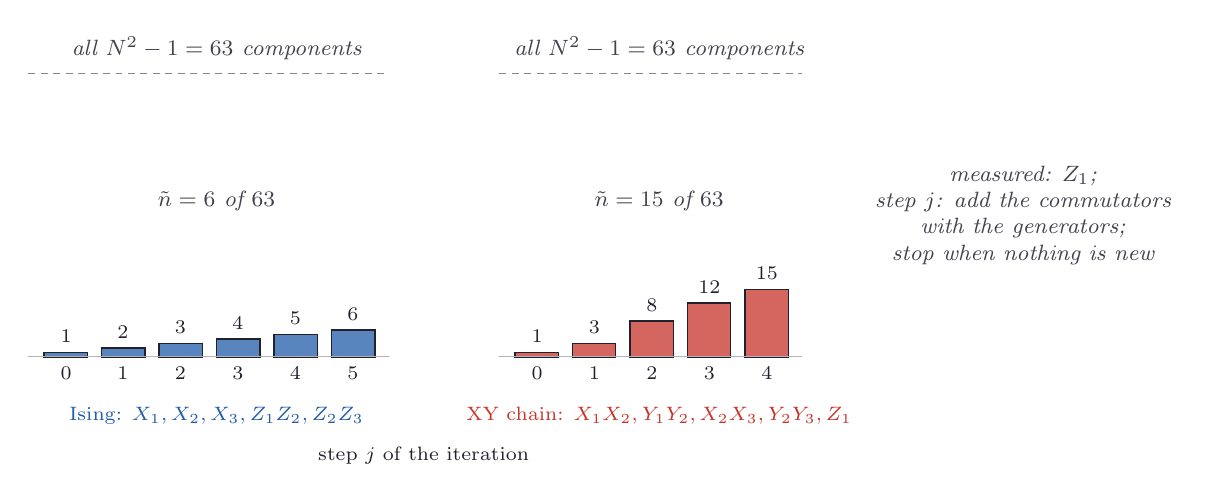
\begin{tikzpicture}[ink/.style={line width=0.9pt, ndInk}, faint/.style={line width=0.4pt, ndInk!35}, dashedink/.style={line width=0.5pt, ndInk!55, dash pattern=on 2.5pt off 2pt}, vec/.style={->, >=stealth, line width=1.2pt}, note/.style={font=\footnotesize\itshape, text=ndInk!85, align=center}, pointer/.style={->, >=stealth, line width=0.4pt, ndInk!60, shorten >=2pt, shorten <=1pt}, dot/.style={circle, fill=ndInk, inner sep=0pt, minimum size=3.4pt}, wash/.style={fill=ndSky, fill opacity=0.55}, every node/.style={text=ndInk}]
\definecolor{ndInk}{rgb}{0.13,0.13,0.18}
\definecolor{ndPaper}{rgb}{0.99,0.96,0.88}
\definecolor{ndSky}{rgb}{0.84,0.91,0.98}
\definecolor{ndRose}{rgb}{0.98,0.86,0.84}
\definecolor{ndBlue}{rgb}{0.13,0.36,0.66}
\definecolor{ndRed}{rgb}{0.78,0.20,0.16}
\definecolor{ndGold}{rgb}{0.88,0.62,0.10}
\definecolor{ndGreen}{rgb}{0.18,0.52,0.30}
\fill[ndBlue, fill opacity=0.75] (0.00,0) rectangle (0.55,0.057);
\draw[ink, line width=0.5pt] (0.00,0) rectangle (0.55,0.057);
\node[font=\scriptsize, above] at (0.28,0.057) {1};
\node[font=\scriptsize, below] at (0.28,0) {0};
\fill[ndBlue, fill opacity=0.75] (0.73,0) rectangle (1.28,0.114);
\draw[ink, line width=0.5pt] (0.73,0) rectangle (1.28,0.114);
\node[font=\scriptsize, above] at (1.00,0.114) {2};
\node[font=\scriptsize, below] at (1.00,0) {1};
\fill[ndBlue, fill opacity=0.75] (1.46,0) rectangle (2.01,0.171);
\draw[ink, line width=0.5pt] (1.46,0) rectangle (2.01,0.171);
\node[font=\scriptsize, above] at (1.73,0.171) {3};
\node[font=\scriptsize, below] at (1.73,0) {2};
\fill[ndBlue, fill opacity=0.75] (2.19,0) rectangle (2.74,0.229);
\draw[ink, line width=0.5pt] (2.19,0) rectangle (2.74,0.229);
\node[font=\scriptsize, above] at (2.46,0.229) {4};
\node[font=\scriptsize, below] at (2.46,0) {3};
\fill[ndBlue, fill opacity=0.75] (2.92,0) rectangle (3.47,0.286);
\draw[ink, line width=0.5pt] (2.92,0) rectangle (3.47,0.286);
\node[font=\scriptsize, above] at (3.19,0.286) {5};
\node[font=\scriptsize, below] at (3.19,0) {4};
\fill[ndBlue, fill opacity=0.75] (3.65,0) rectangle (4.20,0.343);
\draw[ink, line width=0.5pt] (3.65,0) rectangle (4.20,0.343);
\node[font=\scriptsize, above] at (3.92,0.343) {6};
\node[font=\scriptsize, below] at (3.92,0) {5};
\draw[faint] (-0.20,0) -- (4.38,0);
\draw[dashedink] (-0.20,3.600) -- (4.38,3.600);
\node[note, anchor=south] at (2.19,3.650) {all $N^2-1=63$ components};
\node[font=\scriptsize, text=ndBlue] at (2.19,-0.75) {Ising: $X_1,X_2,X_3,Z_1Z_2,Z_2Z_3$};
\node[note] at (2.19,1.980) {$\tilde n=6$ of $63$};
\fill[ndRed, fill opacity=0.75] (5.98,0) rectangle (6.53,0.057);
\draw[ink, line width=0.5pt] (5.98,0) rectangle (6.53,0.057);
\node[font=\scriptsize, above] at (6.26,0.057) {1};
\node[font=\scriptsize, below] at (6.26,0) {0};
\fill[ndRed, fill opacity=0.75] (6.71,0) rectangle (7.26,0.171);
\draw[ink, line width=0.5pt] (6.71,0) rectangle (7.26,0.171);
\node[font=\scriptsize, above] at (6.99,0.171) {3};
\node[font=\scriptsize, below] at (6.99,0) {1};
\fill[ndRed, fill opacity=0.75] (7.44,0) rectangle (7.99,0.457);
\draw[ink, line width=0.5pt] (7.44,0) rectangle (7.99,0.457);
\node[font=\scriptsize, above] at (7.72,0.457) {8};
\node[font=\scriptsize, below] at (7.72,0) {2};
\fill[ndRed, fill opacity=0.75] (8.17,0) rectangle (8.72,0.686);
\draw[ink, line width=0.5pt] (8.17,0) rectangle (8.72,0.686);
\node[font=\scriptsize, above] at (8.45,0.686) {12};
\node[font=\scriptsize, below] at (8.45,0) {3};
\fill[ndRed, fill opacity=0.75] (8.90,0) rectangle (9.45,0.857);
\draw[ink, line width=0.5pt] (8.90,0) rectangle (9.45,0.857);
\node[font=\scriptsize, above] at (9.18,0.857) {15};
\node[font=\scriptsize, below] at (9.18,0) {4};
\draw[faint] (5.78,0) -- (9.63,0);
\draw[dashedink] (5.78,3.600) -- (9.63,3.600);
\node[note, anchor=south] at (7.81,3.650) {all $N^2-1=63$ components};
\node[font=\scriptsize, text=ndRed] at (7.81,-0.75) {XY chain: $X_1X_2,Y_1Y_2,X_2X_3,Y_2Y_3,Z_1$};
\node[note] at (7.81,1.980) {$\tilde n=15$ of $63$};
\node[note, anchor=west] at (10.43,1.8) {measured: $Z_1$;\\ step $j$: add the commutators\\ with the generators;\\ stop when nothing is new};
\node[font=\scriptsize] at (4.82,-1.25) {step $j$ of the iteration};
\end{tikzpicture}
}
\caption{The size of the accessible set $G_j$ against the step $j$, for three qubits measured through $Z_1$: a transverse-field Ising chain (blue) and an XY chain (red), against all $N^2-1=63$ components (dashed). Generated by \texttt{code/ch03\_accessible.py}.}\label{fig:ch03:accessible}
\end{figure}}
\ona{\endgraf\medskip\noindent\textit{Reading the figure.} The height of a bar is the number of observables, Pauli strings, whose evolution has to be tracked after $j$ steps of the procedure; the dashed line marks all $63$ of them. The procedure stops when a step adds nothing new.\endgraf\smallskip\noindent\textit{Why it matters.} One only needs to model what can influence the measurement. In computer-science terms, the procedure is a breadth-first search on a graph whose vertices are Pauli strings, with an edge between two strings when they anticommute, started from the measured observable. It is the analogue of dependency analysis, or program slicing, which finds the variables that can affect a program's output. For the Ising chain, $63$ unknowns shrink to $6$, which makes simulation and identification much cheaper. Equally important, parameters outside the accessible set cannot be identified from these measurements, however much data is collected.}
\onp{\begin{center}\resizebox{\linewidth}{!}{% Generated by code/needham.py -- do not edit by hand.
\definecolor{qocA}{rgb}{0.00,0.45,0.70}
\definecolor{qocB}{rgb}{0.90,0.60,0.00}
\definecolor{qocC}{rgb}{0.00,0.62,0.45}
\definecolor{qocD}{rgb}{0.80,0.40,0.00}
\definecolor{qocE}{rgb}{0.80,0.60,0.70}
\definecolor{qocF}{rgb}{0.35,0.70,0.90}
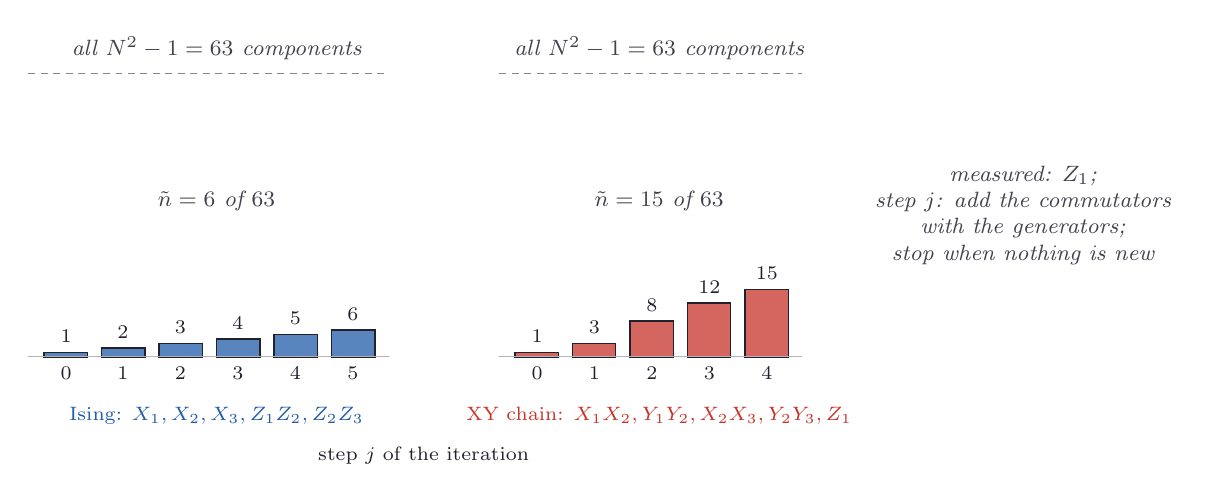
\begin{tikzpicture}[ink/.style={line width=0.9pt, ndInk}, faint/.style={line width=0.4pt, ndInk!35}, dashedink/.style={line width=0.5pt, ndInk!55, dash pattern=on 2.5pt off 2pt}, vec/.style={->, >=stealth, line width=1.2pt}, note/.style={font=\footnotesize\itshape, text=ndInk!85, align=center}, pointer/.style={->, >=stealth, line width=0.4pt, ndInk!60, shorten >=2pt, shorten <=1pt}, dot/.style={circle, fill=ndInk, inner sep=0pt, minimum size=3.4pt}, wash/.style={fill=ndSky, fill opacity=0.55}, every node/.style={text=ndInk}]
\definecolor{ndInk}{rgb}{0.13,0.13,0.18}
\definecolor{ndPaper}{rgb}{0.99,0.96,0.88}
\definecolor{ndSky}{rgb}{0.84,0.91,0.98}
\definecolor{ndRose}{rgb}{0.98,0.86,0.84}
\definecolor{ndBlue}{rgb}{0.13,0.36,0.66}
\definecolor{ndRed}{rgb}{0.78,0.20,0.16}
\definecolor{ndGold}{rgb}{0.88,0.62,0.10}
\definecolor{ndGreen}{rgb}{0.18,0.52,0.30}
\fill[ndBlue, fill opacity=0.75] (0.00,0) rectangle (0.55,0.057);
\draw[ink, line width=0.5pt] (0.00,0) rectangle (0.55,0.057);
\node[font=\scriptsize, above] at (0.28,0.057) {1};
\node[font=\scriptsize, below] at (0.28,0) {0};
\fill[ndBlue, fill opacity=0.75] (0.73,0) rectangle (1.28,0.114);
\draw[ink, line width=0.5pt] (0.73,0) rectangle (1.28,0.114);
\node[font=\scriptsize, above] at (1.00,0.114) {2};
\node[font=\scriptsize, below] at (1.00,0) {1};
\fill[ndBlue, fill opacity=0.75] (1.46,0) rectangle (2.01,0.171);
\draw[ink, line width=0.5pt] (1.46,0) rectangle (2.01,0.171);
\node[font=\scriptsize, above] at (1.73,0.171) {3};
\node[font=\scriptsize, below] at (1.73,0) {2};
\fill[ndBlue, fill opacity=0.75] (2.19,0) rectangle (2.74,0.229);
\draw[ink, line width=0.5pt] (2.19,0) rectangle (2.74,0.229);
\node[font=\scriptsize, above] at (2.46,0.229) {4};
\node[font=\scriptsize, below] at (2.46,0) {3};
\fill[ndBlue, fill opacity=0.75] (2.92,0) rectangle (3.47,0.286);
\draw[ink, line width=0.5pt] (2.92,0) rectangle (3.47,0.286);
\node[font=\scriptsize, above] at (3.19,0.286) {5};
\node[font=\scriptsize, below] at (3.19,0) {4};
\fill[ndBlue, fill opacity=0.75] (3.65,0) rectangle (4.20,0.343);
\draw[ink, line width=0.5pt] (3.65,0) rectangle (4.20,0.343);
\node[font=\scriptsize, above] at (3.92,0.343) {6};
\node[font=\scriptsize, below] at (3.92,0) {5};
\draw[faint] (-0.20,0) -- (4.38,0);
\draw[dashedink] (-0.20,3.600) -- (4.38,3.600);
\node[note, anchor=south] at (2.19,3.650) {all $N^2-1=63$ components};
\node[font=\scriptsize, text=ndBlue] at (2.19,-0.75) {Ising: $X_1,X_2,X_3,Z_1Z_2,Z_2Z_3$};
\node[note] at (2.19,1.980) {$\tilde n=6$ of $63$};
\fill[ndRed, fill opacity=0.75] (5.98,0) rectangle (6.53,0.057);
\draw[ink, line width=0.5pt] (5.98,0) rectangle (6.53,0.057);
\node[font=\scriptsize, above] at (6.26,0.057) {1};
\node[font=\scriptsize, below] at (6.26,0) {0};
\fill[ndRed, fill opacity=0.75] (6.71,0) rectangle (7.26,0.171);
\draw[ink, line width=0.5pt] (6.71,0) rectangle (7.26,0.171);
\node[font=\scriptsize, above] at (6.99,0.171) {3};
\node[font=\scriptsize, below] at (6.99,0) {1};
\fill[ndRed, fill opacity=0.75] (7.44,0) rectangle (7.99,0.457);
\draw[ink, line width=0.5pt] (7.44,0) rectangle (7.99,0.457);
\node[font=\scriptsize, above] at (7.72,0.457) {8};
\node[font=\scriptsize, below] at (7.72,0) {2};
\fill[ndRed, fill opacity=0.75] (8.17,0) rectangle (8.72,0.686);
\draw[ink, line width=0.5pt] (8.17,0) rectangle (8.72,0.686);
\node[font=\scriptsize, above] at (8.45,0.686) {12};
\node[font=\scriptsize, below] at (8.45,0) {3};
\fill[ndRed, fill opacity=0.75] (8.90,0) rectangle (9.45,0.857);
\draw[ink, line width=0.5pt] (8.90,0) rectangle (9.45,0.857);
\node[font=\scriptsize, above] at (9.18,0.857) {15};
\node[font=\scriptsize, below] at (9.18,0) {4};
\draw[faint] (5.78,0) -- (9.63,0);
\draw[dashedink] (5.78,3.600) -- (9.63,3.600);
\node[note, anchor=south] at (7.81,3.650) {all $N^2-1=63$ components};
\node[font=\scriptsize, text=ndRed] at (7.81,-0.75) {XY chain: $X_1X_2,Y_1Y_2,X_2X_3,Y_2Y_3,Z_1$};
\node[note] at (7.81,1.980) {$\tilde n=15$ of $63$};
\node[note, anchor=west] at (10.43,1.8) {measured: $Z_1$;\\ step $j$: add the commutators\\ with the generators;\\ stop when nothing is new};
\node[font=\scriptsize] at (4.82,-1.25) {step $j$ of the iteration};
\end{tikzpicture}
}\end{center}}
\end{frame}

\section{The random Schr\"odinger equation}

\begin{frame}\ft{Random ordinary differential equations}
\ona{The GKSL equation describes the \emph{average} effect of an environment. A complementary, intermediate model keeps every realisation unitary and puts the randomness into the Hamiltonian. The framework is that of random ordinary differential equations (RODEs), see the monograph of Han and Kloeden and the classical paper of Strand (1970).\citep{HanandKloeden,strand1970random}}
\begin{defn}[RODE]\label{def:ch03:rode}
Let $\eta:[0,T] \times \Omega \rightarrow \R^m$ be a random process on a probability space $(\Omega, \mathcal{F}, \Prob)$, and $f:[0,T] \times \R^n \times \R^m\rightarrow \R^n$ continuous. A random differential equation is an equation of the form
\begin{equation}\label{eq:ch03:RODEmain}
    \dd{t}x(t, \cdot) = f(t, x(t, \cdot),\eta(t, \cdot)), \qquad x(0, \cdot) = x_0 .
\end{equation}
It is linear if $f$ is linear in the state; any linear RODE can be written as $\dd{t}x(t, \cdot) = A(t, \cdot)x(t, \cdot)$ with a matrix-valued random process $A$.
\end{defn}
\ona{A random process $x(t,\omega)$ is a \emph{sample path solution} if, for almost all $\omega$, $x(\cdot,\omega)$ is absolutely continuous and satisfies \eqref{eq:ch03:RODEmain} for almost all $t$. Unlike stochastic differential equations, RODEs are solved pathwise by ordinary calculus; the noise enters as a parameter, not through an It\^o integral, and no white-noise idealisation is needed.}
\onp{\begin{itemize}\item Solved \emph{pathwise} by ordinary calculus, one $\omega$ at a time. \item No It\^o calculus, no white noise: $\eta(\cdot,\omega)$ is an ordinary (rough) function. \item Averages over $\omega$ recover mixed-state behaviour.\end{itemize}}
\end{frame}

\begin{frame}\ft{The random Schr\"odinger equation}
\ona{The RODE of interest is the \emph{random Schr\"odinger equation} for the time evolution operator,}
\begin{equation}\label{eq:ch03:rse}
    \dd{t}U(t, \cdot) = -\imath \big(H_{0}(t) + H_{1}(t, \cdot)\big) U(t, \cdot),\qquad U(0, \cdot) = \Id,
\end{equation}
\ona{where $H_{0}(t)$ is the deterministic part of the Hamiltonian, while $H_{1}(t,\cdot)$ is a Hermitian matrix-valued random process, assumed essentially bounded and centred (any drift can be absorbed into $H_0$). The corresponding equation for random states, $\dd{t}\ket{\varphi(t,\cdot)}=-\imath(H_0+H_1)\ket{\varphi(t,\cdot)}$, is related to it pathwise by $\ket{\varphi(t,\omega)}=U(t,\omega)\ket{\varphi_0(\omega)}$. Since $H_0+H_1(t,\omega)$ is Hermitian, the sample trajectories $U(t,\omega)$ are always unitary. However, by considering ensemble averages over $\Omega$, we obtain the mixed-state behaviour that we expect open quantum systems to exhibit.}
\onp{$H_0$ deterministic, $H_1(t,\omega)$ a bounded, centred Hermitian random process. Each sample path is unitary; the \alert{ensemble average is mixed}.}
\begin{propn}[Mixed-state behaviour]\label{prop:ch03:mixed}
Let $\psi\in L^2(\Omega,\Hil)$ be a normalised random state and $\rho(\omega)=\ket{\psi(\omega)}\bra{\psi(\omega)}$. Then $\hat\rho=\Expect_\omega\rho(\omega)$ is a density matrix, and it is mixed as soon as $\rho(\omega)$ is non-constant.
\end{propn}
\ona{\begin{pf}
$\Tr\hat\rho=1$ and $\hat\rho\succeq0$ by linearity. $\rho(\omega)$ is supported on the pure states $\Dens[\Hil]\cap\{\Tr\rho^2=1\}$, and the expectation lies in the convex hull of the support. Since the set of pure states contains no non-trivial convex subsets, $\Expect\rho$ is mixed unless $\rho$ is almost surely constant.
\end{pf}}
\onp{Proof: $\Expect\rho$ lies in the convex hull of the support; pure states contain no non-trivial segments.}
\end{frame}

\begin{frame}\ft{Sample paths versus the ensemble}
\ona{Figure~\ref{fig:ch03:rse} illustrates Proposition~\ref{prop:ch03:mixed} for a qubit with $H_0=\tfrac12\sigma_z+\tfrac12\sigma_x$ and a random dephasing term $H_1=\tfrac12 b(t,\omega)\sigma_z$, where $b$ is an Ornstein--Uhlenbeck process (correlation time $0.5$, unit variance). Each sample path keeps oscillating and stays pure, but different paths drift apart in phase; the ensemble mean of $\langle\sigma_x\rangle$ is therefore damped, and the purity of $\hat\rho$ decays towards its minimum $\tfrac12$, exactly as under the dephasing Lindbladian of Figure~\ref{fig:ch03:decoherence}. Trajectories of this kind, for Gaussian noise with Mat\'ern covariance, are studied in \cite{Parvaiz2025}.}
\ona{\begin{figure}[H]\centering
\resizebox{\linewidth}{!}{% Generated by code/needham.py -- do not edit by hand.
\definecolor{qocA}{rgb}{0.00,0.45,0.70}
\definecolor{qocB}{rgb}{0.90,0.60,0.00}
\definecolor{qocC}{rgb}{0.00,0.62,0.45}
\definecolor{qocD}{rgb}{0.80,0.40,0.00}
\definecolor{qocE}{rgb}{0.80,0.60,0.70}
\definecolor{qocF}{rgb}{0.35,0.70,0.90}
\begin{tikzpicture}[ink/.style={line width=0.9pt, ndInk}, faint/.style={line width=0.4pt, ndInk!35}, dashedink/.style={line width=0.5pt, ndInk!55, dash pattern=on 2.5pt off 2pt}, vec/.style={->, >=stealth, line width=1.2pt}, note/.style={font=\footnotesize\itshape, text=ndInk!85, align=center}, pointer/.style={->, >=stealth, line width=0.4pt, ndInk!60, shorten >=2pt, shorten <=1pt}, dot/.style={circle, fill=ndInk, inner sep=0pt, minimum size=3.4pt}, wash/.style={fill=ndSky, fill opacity=0.55}, every node/.style={text=ndInk}]
\definecolor{ndInk}{rgb}{0.13,0.13,0.18}
\definecolor{ndPaper}{rgb}{0.99,0.96,0.88}
\definecolor{ndSky}{rgb}{0.84,0.91,0.98}
\definecolor{ndRose}{rgb}{0.98,0.86,0.84}
\definecolor{ndBlue}{rgb}{0.13,0.36,0.66}
\definecolor{ndRed}{rgb}{0.78,0.20,0.16}
\definecolor{ndGold}{rgb}{0.88,0.62,0.10}
\definecolor{ndGreen}{rgb}{0.18,0.52,0.30}
\draw[faint, ->, >=stealth] (0.000,2.149) -- (8.320,2.149) node[right, text=ndInk] {$t$};
\draw[faint, ->, >=stealth] (0.000,0.000) -- (0.000,4.664) node[above, text=ndInk] {$\langle\sigma_x\rangle$};
\draw[faint] (0.060,0.102) -- (-0.060,0.102) node[left, font=\scriptsize, text=ndInk] {$-1$};
\draw[faint] (0.060,2.149) -- (-0.060,2.149) node[left, font=\scriptsize, text=ndInk] {$0$};
\draw[faint] (0.060,4.195) -- (-0.060,4.195) node[left, font=\scriptsize, text=ndInk] {$1$};
\draw[line width=0.7pt, ndGold] (0.000,2.149) -- (0.020,2.150) -- (0.040,2.152) -- (0.060,2.156) -- (0.080,2.159) -- (0.100,2.165) -- (0.120,2.168) -- (0.140,2.175) -- (0.160,2.182) -- (0.180,2.190) -- (0.201,2.199) -- (0.221,2.215) -- (0.241,2.223) -- (0.261,2.230) -- (0.281,2.236) -- (0.301,2.250) -- (0.321,2.258) -- (0.341,2.266) -- (0.361,2.270) -- (0.381,2.275) -- (0.401,2.285) -- (0.421,2.288) -- (0.441,2.302) -- (0.461,2.324) -- (0.481,2.351) -- (0.501,2.388) -- (0.521,2.419) -- (0.541,2.449) -- (0.561,2.471) -- (0.581,2.492) -- (0.602,2.519) -- (0.622,2.540) -- (0.642,2.558) -- (0.662,2.570) -- (0.682,2.573) -- (0.702,2.571) -- (0.722,2.570) -- (0.742,2.558) -- (0.762,2.551) -- (0.782,2.567) -- (0.802,2.594) -- (0.822,2.619) -- (0.842,2.634) -- (0.862,2.641) -- (0.882,2.672) -- (0.902,2.704) -- (0.922,2.729) -- (0.942,2.758) -- (0.962,2.816) -- (0.982,2.875) -- (1.003,2.941) -- (1.023,3.010) -- (1.043,3.073) -- (1.063,3.118) -- (1.083,3.159) -- (1.103,3.197) -- (1.123,3.242) -- (1.143,3.298) -- (1.163,3.363) -- (1.183,3.429) -- (1.203,3.503) -- (1.223,3.563) -- (1.243,3.634) -- (1.263,3.705) -- (1.283,3.768) -- (1.303,3.830) -- (1.323,3.885) -- (1.343,3.944) -- (1.363,4.006) -- (1.383,4.070) -- (1.404,4.114) -- (1.424,4.143) -- (1.444,4.163) -- (1.464,4.179) -- (1.484,4.190) -- (1.504,4.195) -- (1.524,4.194) -- (1.544,4.191) -- (1.564,4.184) -- (1.584,4.173) -- (1.604,4.156) -- (1.624,4.136) -- (1.644,4.113) -- (1.664,4.086) -- (1.684,4.054) -- (1.704,4.018) -- (1.724,3.978) -- (1.744,3.940) -- (1.764,3.897) -- (1.784,3.852) -- (1.805,3.793) -- (1.825,3.721) -- (1.845,3.644) -- (1.865,3.569) -- (1.885,3.499) -- (1.905,3.424) -- (1.925,3.347) -- (1.945,3.274) -- (1.965,3.200) -- (1.985,3.134) -- (2.005,3.060) -- (2.025,2.992) -- (2.045,2.907) -- (2.065,2.818) -- (2.085,2.722) -- (2.105,2.643) -- (2.125,2.564) -- (2.145,2.476) -- (2.165,2.403) -- (2.185,2.337) -- (2.206,2.271) -- (2.226,2.226) -- (2.246,2.177) -- (2.266,2.119) -- (2.286,2.073) -- (2.306,2.024) -- (2.326,1.992) -- (2.346,1.961) -- (2.366,1.950) -- (2.386,1.925) -- (2.406,1.895) -- (2.426,1.866) -- (2.446,1.846) -- (2.466,1.812) -- (2.486,1.760) -- (2.506,1.729) -- (2.526,1.688) -- (2.546,1.635) -- (2.566,1.584) -- (2.586,1.546) -- (2.607,1.506) -- (2.627,1.470) -- (2.647,1.441) -- (2.667,1.423) -- (2.687,1.403) -- (2.707,1.382) -- (2.727,1.366) -- (2.747,1.351) -- (2.767,1.341) -- (2.787,1.332) -- (2.807,1.324) -- (2.827,1.320) -- (2.847,1.317) -- (2.867,1.317) -- (2.887,1.319) -- (2.907,1.326) -- (2.927,1.336) -- (2.947,1.350) -- (2.967,1.368) -- (2.987,1.392) -- (3.008,1.421) -- (3.028,1.453) -- (3.048,1.473) -- (3.068,1.502) -- (3.088,1.547) -- (3.108,1.598) -- (3.128,1.651) -- (3.148,1.705) -- (3.168,1.760) -- (3.188,1.817) -- (3.208,1.863) -- (3.228,1.906) -- (3.248,1.939) -- (3.268,1.976) -- (3.288,2.011) -- (3.308,2.053) -- (3.328,2.093) -- (3.348,2.146) -- (3.368,2.201) -- (3.388,2.285) -- (3.409,2.343) -- (3.429,2.394) -- (3.449,2.456) -- (3.469,2.550) -- (3.489,2.640) -- (3.509,2.727) -- (3.529,2.809) -- (3.549,2.906) -- (3.569,2.996) -- (3.589,3.090) -- (3.609,3.176) -- (3.629,3.243) -- (3.649,3.311) -- (3.669,3.382) -- (3.689,3.464) -- (3.709,3.539) -- (3.729,3.603) -- (3.749,3.669) -- (3.769,3.732) -- (3.789,3.792) -- (3.810,3.847) -- (3.830,3.905) -- (3.850,3.960) -- (3.870,4.018) -- (3.890,4.071) -- (3.910,4.114) -- (3.930,4.140) -- (3.950,4.158) -- (3.970,4.168) -- (3.990,4.168) -- (4.010,4.157) -- (4.030,4.136) -- (4.050,4.102) -- (4.070,4.062) -- (4.090,4.003) -- (4.110,3.944) -- (4.130,3.893) -- (4.150,3.852) -- (4.170,3.817) -- (4.190,3.791) -- (4.211,3.747) -- (4.231,3.704) -- (4.251,3.674) -- (4.271,3.633) -- (4.291,3.596) -- (4.311,3.572) -- (4.331,3.538) -- (4.351,3.497) -- (4.371,3.461) -- (4.391,3.409) -- (4.411,3.356) -- (4.431,3.284) -- (4.451,3.207) -- (4.471,3.111) -- (4.491,3.015) -- (4.511,2.935) -- (4.531,2.826) -- (4.551,2.726) -- (4.571,2.630) -- (4.591,2.547) -- (4.612,2.468) -- (4.632,2.389) -- (4.652,2.311) -- (4.672,2.228) -- (4.692,2.127) -- (4.712,2.034) -- (4.732,1.959) -- (4.752,1.902) -- (4.772,1.854) -- (4.792,1.825) -- (4.812,1.790) -- (4.832,1.760) -- (4.852,1.735) -- (4.872,1.710) -- (4.892,1.698) -- (4.912,1.692) -- (4.932,1.681) -- (4.952,1.666) -- (4.972,1.654) -- (4.992,1.631) -- (5.013,1.617) -- (5.033,1.606) -- (5.053,1.597) -- (5.073,1.601) -- (5.093,1.596) -- (5.113,1.589) -- (5.133,1.587) -- (5.153,1.578) -- (5.173,1.570) -- (5.193,1.563) -- (5.213,1.559) -- (5.233,1.556) -- (5.253,1.556) -- (5.273,1.556) -- (5.293,1.558) -- (5.313,1.561) -- (5.333,1.567) -- (5.353,1.576) -- (5.373,1.587) -- (5.393,1.602) -- (5.414,1.615) -- (5.434,1.634) -- (5.454,1.663) -- (5.474,1.698) -- (5.494,1.741) -- (5.514,1.781) -- (5.534,1.816) -- (5.554,1.844) -- (5.574,1.881) -- (5.594,1.919) -- (5.614,1.969) -- (5.634,2.014) -- (5.654,2.056) -- (5.674,2.099) -- (5.694,2.153) -- (5.714,2.207) -- (5.734,2.265) -- (5.754,2.322) -- (5.774,2.382) -- (5.794,2.429) -- (5.815,2.478) -- (5.835,2.524) -- (5.855,2.570) -- (5.875,2.622) -- (5.895,2.666) -- (5.915,2.709) -- (5.935,2.749) -- (5.955,2.794) -- (5.975,2.848) -- (5.995,2.891) -- (6.015,2.940) -- (6.035,3.015) -- (6.055,3.070) -- (6.075,3.113) -- (6.095,3.145) -- (6.115,3.174) -- (6.135,3.224) -- (6.155,3.272) -- (6.175,3.312) -- (6.195,3.358) -- (6.216,3.397) -- (6.236,3.448) -- (6.256,3.500) -- (6.276,3.566) -- (6.296,3.621) -- (6.316,3.703) -- (6.336,3.785) -- (6.356,3.864) -- (6.376,3.932) -- (6.396,3.986) -- (6.416,4.028) -- (6.436,4.063) -- (6.456,4.090) -- (6.476,4.114) -- (6.496,4.132) -- (6.516,4.149) -- (6.536,4.165) -- (6.556,4.175) -- (6.576,4.183) -- (6.596,4.187) -- (6.617,4.186) -- (6.637,4.179) -- (6.657,4.164) -- (6.677,4.145) -- (6.697,4.122) -- (6.717,4.088) -- (6.737,4.052) -- (6.757,4.024) -- (6.777,4.007) -- (6.797,4.005) -- (6.817,4.015) -- (6.837,4.026) -- (6.857,4.027) -- (6.877,4.031) -- (6.897,4.031) -- (6.917,4.031) -- (6.937,4.030) -- (6.957,4.029) -- (6.977,4.029) -- (6.997,4.025) -- (7.018,4.027) -- (7.038,4.022) -- (7.058,4.013) -- (7.078,4.004) -- (7.098,3.990) -- (7.118,3.979) -- (7.138,3.971) -- (7.158,3.961) -- (7.178,3.952) -- (7.198,3.945) -- (7.218,3.941) -- (7.238,3.940) -- (7.258,3.932) -- (7.278,3.935) -- (7.298,3.935) -- (7.318,3.935) -- (7.338,3.931) -- (7.358,3.924) -- (7.378,3.930) -- (7.398,3.932) -- (7.419,3.931) -- (7.439,3.930) -- (7.459,3.931) -- (7.479,3.927) -- (7.499,3.924) -- (7.519,3.914) -- (7.539,3.901) -- (7.559,3.878) -- (7.579,3.858) -- (7.599,3.845) -- (7.619,3.828) -- (7.639,3.807) -- (7.659,3.784) -- (7.679,3.769) -- (7.699,3.757) -- (7.719,3.741) -- (7.739,3.726) -- (7.759,3.711) -- (7.779,3.697) -- (7.799,3.688) -- (7.820,3.682) -- (7.840,3.683) -- (7.860,3.674) -- (7.880,3.667) -- (7.900,3.657) -- (7.920,3.652) -- (7.940,3.643) -- (7.960,3.643) -- (7.980,3.638) -- (8.000,3.633);
\draw[line width=0.7pt, ndGreen] (0.000,2.149) -- (0.020,2.150) -- (0.040,2.152) -- (0.060,2.156) -- (0.080,2.162) -- (0.100,2.172) -- (0.120,2.183) -- (0.140,2.195) -- (0.160,2.203) -- (0.180,2.210) -- (0.201,2.219) -- (0.221,2.233) -- (0.241,2.248) -- (0.261,2.273) -- (0.281,2.309) -- (0.301,2.346) -- (0.321,2.369) -- (0.341,2.384) -- (0.361,2.394) -- (0.381,2.413) -- (0.401,2.435) -- (0.421,2.442) -- (0.441,2.449) -- (0.461,2.471) -- (0.481,2.490) -- (0.501,2.503) -- (0.521,2.536) -- (0.541,2.570) -- (0.561,2.601) -- (0.581,2.635) -- (0.602,2.670) -- (0.622,2.701) -- (0.642,2.745) -- (0.662,2.800) -- (0.682,2.863) -- (0.702,2.923) -- (0.722,2.994) -- (0.742,3.061) -- (0.762,3.131) -- (0.782,3.207) -- (0.802,3.287) -- (0.822,3.378) -- (0.842,3.465) -- (0.862,3.530) -- (0.882,3.581) -- (0.902,3.638) -- (0.922,3.688) -- (0.942,3.735) -- (0.962,3.773) -- (0.982,3.812) -- (1.003,3.845) -- (1.023,3.880) -- (1.043,3.907) -- (1.063,3.932) -- (1.083,3.953) -- (1.103,3.965) -- (1.123,3.974) -- (1.143,3.976) -- (1.163,3.975) -- (1.183,3.969) -- (1.203,3.961) -- (1.223,3.952) -- (1.243,3.942) -- (1.263,3.933) -- (1.283,3.920) -- (1.303,3.903) -- (1.323,3.886) -- (1.343,3.867) -- (1.363,3.845) -- (1.383,3.814) -- (1.404,3.775) -- (1.424,3.736) -- (1.444,3.690) -- (1.464,3.643) -- (1.484,3.596) -- (1.504,3.533) -- (1.524,3.471) -- (1.544,3.412) -- (1.564,3.370) -- (1.584,3.340) -- (1.604,3.306) -- (1.624,3.279) -- (1.644,3.247) -- (1.664,3.225) -- (1.684,3.209) -- (1.704,3.188) -- (1.724,3.154) -- (1.744,3.116) -- (1.764,3.069) -- (1.784,3.008) -- (1.805,2.940) -- (1.825,2.881) -- (1.845,2.824) -- (1.865,2.764) -- (1.885,2.709) -- (1.905,2.652) -- (1.925,2.611) -- (1.945,2.578) -- (1.965,2.542) -- (1.985,2.524) -- (2.005,2.515) -- (2.025,2.505) -- (2.045,2.507) -- (2.065,2.507) -- (2.085,2.511) -- (2.105,2.515) -- (2.125,2.519) -- (2.145,2.521) -- (2.165,2.524) -- (2.185,2.526) -- (2.206,2.529) -- (2.226,2.530) -- (2.246,2.526) -- (2.266,2.521) -- (2.286,2.517) -- (2.306,2.515) -- (2.326,2.513) -- (2.346,2.512) -- (2.366,2.512) -- (2.386,2.512) -- (2.406,2.512) -- (2.426,2.513) -- (2.446,2.517) -- (2.466,2.521) -- (2.486,2.527) -- (2.506,2.537) -- (2.526,2.550) -- (2.546,2.565) -- (2.566,2.585) -- (2.586,2.604) -- (2.607,2.625) -- (2.627,2.652) -- (2.647,2.683) -- (2.667,2.711) -- (2.687,2.738) -- (2.707,2.767) -- (2.727,2.794) -- (2.747,2.819) -- (2.767,2.847) -- (2.787,2.872) -- (2.807,2.892) -- (2.827,2.913) -- (2.847,2.932) -- (2.867,2.949) -- (2.887,2.960) -- (2.907,2.976) -- (2.927,2.982) -- (2.947,2.981) -- (2.967,2.979) -- (2.987,2.985) -- (3.008,3.000) -- (3.028,3.008) -- (3.048,3.016) -- (3.068,3.016) -- (3.088,3.023) -- (3.108,3.020) -- (3.128,3.018) -- (3.148,3.025) -- (3.168,3.032) -- (3.188,3.052) -- (3.208,3.065) -- (3.228,3.082) -- (3.248,3.108) -- (3.268,3.133) -- (3.288,3.171) -- (3.308,3.213) -- (3.328,3.240) -- (3.348,3.302) -- (3.368,3.366) -- (3.388,3.427) -- (3.409,3.473) -- (3.429,3.517) -- (3.449,3.556) -- (3.469,3.598) -- (3.489,3.640) -- (3.509,3.691) -- (3.529,3.738) -- (3.549,3.782) -- (3.569,3.823) -- (3.589,3.857) -- (3.609,3.885) -- (3.629,3.912) -- (3.649,3.934) -- (3.669,3.949) -- (3.689,3.957) -- (3.709,3.962) -- (3.729,3.964) -- (3.749,3.962) -- (3.769,3.953) -- (3.789,3.941) -- (3.810,3.923) -- (3.830,3.910) -- (3.850,3.898) -- (3.870,3.886) -- (3.890,3.871) -- (3.910,3.848) -- (3.930,3.824) -- (3.950,3.791) -- (3.970,3.752) -- (3.990,3.704) -- (4.010,3.656) -- (4.030,3.595) -- (4.050,3.541) -- (4.070,3.481) -- (4.090,3.428) -- (4.110,3.379) -- (4.130,3.343) -- (4.150,3.311) -- (4.170,3.276) -- (4.190,3.242) -- (4.211,3.221) -- (4.231,3.186) -- (4.251,3.149) -- (4.271,3.104) -- (4.291,3.053) -- (4.311,3.009) -- (4.331,2.982) -- (4.351,2.963) -- (4.371,2.935) -- (4.391,2.915) -- (4.411,2.889) -- (4.431,2.869) -- (4.451,2.846) -- (4.471,2.837) -- (4.491,2.819) -- (4.511,2.802) -- (4.531,2.779) -- (4.551,2.756) -- (4.571,2.730) -- (4.591,2.705) -- (4.612,2.677) -- (4.632,2.658) -- (4.652,2.646) -- (4.672,2.632) -- (4.692,2.618) -- (4.712,2.606) -- (4.732,2.595) -- (4.752,2.583) -- (4.772,2.574) -- (4.792,2.565) -- (4.812,2.559) -- (4.832,2.554) -- (4.852,2.548) -- (4.872,2.541) -- (4.892,2.536) -- (4.912,2.532) -- (4.932,2.529) -- (4.952,2.527) -- (4.972,2.527) -- (4.992,2.527) -- (5.013,2.527) -- (5.033,2.527) -- (5.053,2.529) -- (5.073,2.534) -- (5.093,2.542) -- (5.113,2.554) -- (5.133,2.566) -- (5.153,2.579) -- (5.173,2.596) -- (5.193,2.613) -- (5.213,2.632) -- (5.233,2.646) -- (5.253,2.660) -- (5.273,2.664) -- (5.293,2.667) -- (5.313,2.666) -- (5.333,2.669) -- (5.353,2.670) -- (5.373,2.671) -- (5.393,2.681) -- (5.414,2.685) -- (5.434,2.692) -- (5.454,2.686) -- (5.474,2.683) -- (5.494,2.684) -- (5.514,2.693) -- (5.534,2.696) -- (5.554,2.704) -- (5.574,2.715) -- (5.594,2.727) -- (5.614,2.743) -- (5.634,2.763) -- (5.654,2.789) -- (5.674,2.806) -- (5.694,2.811) -- (5.714,2.844) -- (5.734,2.898) -- (5.754,2.937) -- (5.774,2.981) -- (5.794,3.031) -- (5.815,3.088) -- (5.835,3.146) -- (5.855,3.192) -- (5.875,3.235) -- (5.895,3.273) -- (5.915,3.312) -- (5.935,3.347) -- (5.955,3.381) -- (5.975,3.425) -- (5.995,3.480) -- (6.015,3.522) -- (6.035,3.557) -- (6.055,3.585) -- (6.075,3.624) -- (6.095,3.661) -- (6.115,3.709) -- (6.135,3.751) -- (6.155,3.791) -- (6.175,3.818) -- (6.195,3.854) -- (6.216,3.885) -- (6.236,3.904) -- (6.256,3.919) -- (6.276,3.918) -- (6.296,3.918) -- (6.316,3.920) -- (6.336,3.925) -- (6.356,3.941) -- (6.376,3.956) -- (6.396,3.976) -- (6.416,3.997) -- (6.436,4.016) -- (6.456,4.022) -- (6.476,4.034) -- (6.496,4.043) -- (6.516,4.053) -- (6.536,4.056) -- (6.556,4.061) -- (6.576,4.067) -- (6.596,4.074) -- (6.617,4.080) -- (6.637,4.092) -- (6.657,4.108) -- (6.677,4.126) -- (6.697,4.152) -- (6.717,4.171) -- (6.737,4.183) -- (6.757,4.190) -- (6.777,4.194) -- (6.797,4.195) -- (6.817,4.195) -- (6.837,4.194) -- (6.857,4.194) -- (6.877,4.193) -- (6.897,4.193) -- (6.917,4.193) -- (6.937,4.193) -- (6.957,4.193) -- (6.977,4.193) -- (6.997,4.193) -- (7.018,4.193) -- (7.038,4.193) -- (7.058,4.191) -- (7.078,4.189) -- (7.098,4.185) -- (7.118,4.180) -- (7.138,4.174) -- (7.158,4.167) -- (7.178,4.162) -- (7.198,4.159) -- (7.218,4.156) -- (7.238,4.152) -- (7.258,4.143) -- (7.278,4.138) -- (7.298,4.136) -- (7.318,4.127) -- (7.338,4.114) -- (7.358,4.109) -- (7.378,4.101) -- (7.398,4.091) -- (7.419,4.091) -- (7.439,4.092) -- (7.459,4.092) -- (7.479,4.088) -- (7.499,4.080) -- (7.519,4.070) -- (7.539,4.054) -- (7.559,4.037) -- (7.579,4.025) -- (7.599,4.018) -- (7.619,4.007) -- (7.639,4.006) -- (7.659,4.001) -- (7.679,4.002) -- (7.699,4.004) -- (7.719,4.002) -- (7.739,3.992) -- (7.759,3.993) -- (7.779,3.997) -- (7.799,4.000) -- (7.820,4.005) -- (7.840,4.004) -- (7.860,4.012) -- (7.880,4.018) -- (7.900,4.020) -- (7.920,4.021) -- (7.940,4.018) -- (7.960,4.018) -- (7.980,4.014) -- (8.000,4.012);
\draw[line width=0.7pt, ndRose!60!ndRed] (0.000,2.149) -- (0.020,2.150) -- (0.040,2.152) -- (0.060,2.156) -- (0.080,2.163) -- (0.100,2.170) -- (0.120,2.177) -- (0.140,2.185) -- (0.160,2.194) -- (0.180,2.202) -- (0.201,2.218) -- (0.221,2.235) -- (0.241,2.261) -- (0.261,2.286) -- (0.281,2.306) -- (0.301,2.329) -- (0.321,2.349) -- (0.341,2.384) -- (0.361,2.422) -- (0.381,2.469) -- (0.401,2.514) -- (0.421,2.557) -- (0.441,2.600) -- (0.461,2.646) -- (0.481,2.697) -- (0.501,2.748) -- (0.521,2.792) -- (0.541,2.828) -- (0.561,2.863) -- (0.581,2.903) -- (0.602,2.947) -- (0.622,2.990) -- (0.642,3.027) -- (0.662,3.065) -- (0.682,3.108) -- (0.702,3.149) -- (0.722,3.191) -- (0.742,3.230) -- (0.762,3.277) -- (0.782,3.318) -- (0.802,3.359) -- (0.822,3.402) -- (0.842,3.449) -- (0.862,3.504) -- (0.882,3.560) -- (0.902,3.614) -- (0.922,3.655) -- (0.942,3.695) -- (0.962,3.744) -- (0.982,3.781) -- (1.003,3.809) -- (1.023,3.833) -- (1.043,3.856) -- (1.063,3.877) -- (1.083,3.892) -- (1.103,3.903) -- (1.123,3.911) -- (1.143,3.916) -- (1.163,3.913) -- (1.183,3.901) -- (1.203,3.878) -- (1.223,3.845) -- (1.243,3.804) -- (1.263,3.763) -- (1.283,3.715) -- (1.303,3.661) -- (1.323,3.613) -- (1.343,3.567) -- (1.363,3.523) -- (1.383,3.476) -- (1.404,3.430) -- (1.424,3.381) -- (1.444,3.331) -- (1.464,3.272) -- (1.484,3.228) -- (1.504,3.169) -- (1.524,3.099) -- (1.544,3.029) -- (1.564,2.953) -- (1.584,2.874) -- (1.604,2.803) -- (1.624,2.732) -- (1.644,2.657) -- (1.664,2.581) -- (1.684,2.498) -- (1.704,2.419) -- (1.724,2.342) -- (1.744,2.277) -- (1.764,2.219) -- (1.784,2.167) -- (1.805,2.106) -- (1.825,2.048) -- (1.845,2.002) -- (1.865,1.957) -- (1.885,1.917) -- (1.905,1.898) -- (1.925,1.878) -- (1.945,1.867) -- (1.965,1.855) -- (1.985,1.847) -- (2.005,1.845) -- (2.025,1.842) -- (2.045,1.842) -- (2.065,1.844) -- (2.085,1.844) -- (2.105,1.843) -- (2.125,1.841) -- (2.145,1.840) -- (2.165,1.840) -- (2.185,1.840) -- (2.206,1.841) -- (2.226,1.845) -- (2.246,1.850) -- (2.266,1.859) -- (2.286,1.873) -- (2.306,1.886) -- (2.326,1.902) -- (2.346,1.923) -- (2.366,1.948) -- (2.386,1.976) -- (2.406,2.006) -- (2.426,2.036) -- (2.446,2.061) -- (2.466,2.093) -- (2.486,2.123) -- (2.506,2.164) -- (2.526,2.210) -- (2.546,2.251) -- (2.566,2.291) -- (2.586,2.329) -- (2.607,2.360) -- (2.627,2.397) -- (2.647,2.430) -- (2.667,2.480) -- (2.687,2.537) -- (2.707,2.586) -- (2.727,2.634) -- (2.747,2.681) -- (2.767,2.711) -- (2.787,2.751) -- (2.807,2.802) -- (2.827,2.862) -- (2.847,2.916) -- (2.867,2.981) -- (2.887,3.041) -- (2.907,3.110) -- (2.927,3.194) -- (2.947,3.275) -- (2.967,3.338) -- (2.987,3.395) -- (3.008,3.455) -- (3.028,3.522) -- (3.048,3.575) -- (3.068,3.623) -- (3.088,3.671) -- (3.108,3.718) -- (3.128,3.768) -- (3.148,3.807) -- (3.168,3.840) -- (3.188,3.877) -- (3.208,3.911) -- (3.228,3.944) -- (3.248,3.976) -- (3.268,4.003) -- (3.288,4.025) -- (3.308,4.040) -- (3.328,4.048) -- (3.348,4.053) -- (3.368,4.056) -- (3.388,4.057) -- (3.409,4.057) -- (3.429,4.056) -- (3.449,4.055) -- (3.469,4.053) -- (3.489,4.050) -- (3.509,4.048) -- (3.529,4.048) -- (3.549,4.047) -- (3.569,4.045) -- (3.589,4.046) -- (3.609,4.046) -- (3.629,4.046) -- (3.649,4.047) -- (3.669,4.047) -- (3.689,4.046) -- (3.709,4.046) -- (3.729,4.046) -- (3.749,4.046) -- (3.769,4.046) -- (3.789,4.047) -- (3.810,4.048) -- (3.830,4.049) -- (3.850,4.049) -- (3.870,4.050) -- (3.890,4.051) -- (3.910,4.053) -- (3.930,4.055) -- (3.950,4.058) -- (3.970,4.059) -- (3.990,4.060) -- (4.010,4.060) -- (4.030,4.061) -- (4.050,4.062) -- (4.070,4.062) -- (4.090,4.062) -- (4.110,4.062) -- (4.130,4.061) -- (4.150,4.060) -- (4.170,4.056) -- (4.190,4.051) -- (4.211,4.046) -- (4.231,4.043) -- (4.251,4.045) -- (4.271,4.049) -- (4.291,4.049) -- (4.311,4.045) -- (4.331,4.046) -- (4.351,4.052) -- (4.371,4.057) -- (4.391,4.064) -- (4.411,4.067) -- (4.431,4.064) -- (4.451,4.058) -- (4.471,4.050) -- (4.491,4.041) -- (4.511,4.031) -- (4.531,4.019) -- (4.551,4.011) -- (4.571,4.012) -- (4.591,4.014) -- (4.612,4.027) -- (4.632,4.037) -- (4.652,4.044) -- (4.672,4.054) -- (4.692,4.062) -- (4.712,4.075) -- (4.732,4.085) -- (4.752,4.100) -- (4.772,4.114) -- (4.792,4.135) -- (4.812,4.149) -- (4.832,4.160) -- (4.852,4.167) -- (4.872,4.170) -- (4.892,4.172) -- (4.912,4.173) -- (4.932,4.171) -- (4.952,4.169) -- (4.972,4.168) -- (4.992,4.166) -- (5.013,4.162) -- (5.033,4.155) -- (5.053,4.147) -- (5.073,4.140) -- (5.093,4.134) -- (5.113,4.133) -- (5.133,4.133) -- (5.153,4.130) -- (5.173,4.122) -- (5.193,4.112) -- (5.213,4.095) -- (5.233,4.075) -- (5.253,4.051) -- (5.273,4.027) -- (5.293,3.999) -- (5.313,3.971) -- (5.333,3.943) -- (5.353,3.918) -- (5.373,3.890) -- (5.393,3.861) -- (5.414,3.843) -- (5.434,3.826) -- (5.454,3.815) -- (5.474,3.819) -- (5.494,3.818) -- (5.514,3.804) -- (5.534,3.771) -- (5.554,3.725) -- (5.574,3.685) -- (5.594,3.634) -- (5.614,3.572) -- (5.634,3.528) -- (5.654,3.474) -- (5.674,3.415) -- (5.694,3.353) -- (5.714,3.288) -- (5.734,3.223) -- (5.754,3.140) -- (5.774,3.062) -- (5.794,2.988) -- (5.815,2.914) -- (5.835,2.839) -- (5.855,2.786) -- (5.875,2.718) -- (5.895,2.649) -- (5.915,2.576) -- (5.935,2.503) -- (5.955,2.435) -- (5.975,2.373) -- (5.995,2.313) -- (6.015,2.254) -- (6.035,2.185) -- (6.055,2.117) -- (6.075,2.055) -- (6.095,1.978) -- (6.115,1.917) -- (6.135,1.873) -- (6.155,1.828) -- (6.175,1.789) -- (6.195,1.765) -- (6.216,1.744) -- (6.236,1.730) -- (6.256,1.709) -- (6.276,1.694) -- (6.296,1.674) -- (6.316,1.655) -- (6.336,1.639) -- (6.356,1.625) -- (6.376,1.613) -- (6.396,1.607) -- (6.416,1.603) -- (6.436,1.599) -- (6.456,1.596) -- (6.476,1.594) -- (6.496,1.594) -- (6.516,1.595) -- (6.536,1.598) -- (6.556,1.602) -- (6.576,1.608) -- (6.596,1.614) -- (6.617,1.622) -- (6.637,1.631) -- (6.657,1.642) -- (6.677,1.646) -- (6.697,1.651) -- (6.717,1.668) -- (6.737,1.686) -- (6.757,1.708) -- (6.777,1.728) -- (6.797,1.751) -- (6.817,1.777) -- (6.837,1.802) -- (6.857,1.835) -- (6.877,1.862) -- (6.897,1.889) -- (6.917,1.922) -- (6.937,1.953) -- (6.957,1.974) -- (6.977,2.001) -- (6.997,2.019) -- (7.018,2.033) -- (7.038,2.040) -- (7.058,2.047) -- (7.078,2.051) -- (7.098,2.050) -- (7.118,2.061) -- (7.138,2.094) -- (7.158,2.125) -- (7.178,2.163) -- (7.198,2.197) -- (7.218,2.234) -- (7.238,2.286) -- (7.258,2.340) -- (7.278,2.383) -- (7.298,2.415) -- (7.318,2.440) -- (7.338,2.466) -- (7.358,2.506) -- (7.378,2.527) -- (7.398,2.533) -- (7.419,2.528) -- (7.439,2.500) -- (7.459,2.495) -- (7.479,2.492) -- (7.499,2.521) -- (7.519,2.529) -- (7.539,2.559) -- (7.559,2.579) -- (7.579,2.594) -- (7.599,2.596) -- (7.619,2.585) -- (7.639,2.557) -- (7.659,2.536) -- (7.679,2.498) -- (7.699,2.461) -- (7.719,2.427) -- (7.739,2.408) -- (7.759,2.395) -- (7.779,2.389) -- (7.799,2.394) -- (7.820,2.401) -- (7.840,2.415) -- (7.860,2.417) -- (7.880,2.408) -- (7.900,2.432) -- (7.920,2.456) -- (7.940,2.470) -- (7.960,2.506) -- (7.980,2.540) -- (8.000,2.565);
\draw[line width=2.0pt, ndBlue] (0.000,2.149) -- (0.020,2.149) -- (0.040,2.151) -- (0.060,2.155) -- (0.080,2.159) -- (0.100,2.166) -- (0.120,2.173) -- (0.140,2.181) -- (0.160,2.191) -- (0.180,2.202) -- (0.201,2.214) -- (0.221,2.227) -- (0.241,2.242) -- (0.261,2.257) -- (0.281,2.274) -- (0.301,2.291) -- (0.321,2.309) -- (0.341,2.328) -- (0.361,2.348) -- (0.381,2.370) -- (0.401,2.392) -- (0.421,2.414) -- (0.441,2.437) -- (0.461,2.460) -- (0.481,2.484) -- (0.501,2.510) -- (0.521,2.536) -- (0.541,2.562) -- (0.561,2.587) -- (0.581,2.613) -- (0.602,2.640) -- (0.622,2.667) -- (0.642,2.693) -- (0.662,2.720) -- (0.682,2.747) -- (0.702,2.774) -- (0.722,2.801) -- (0.742,2.829) -- (0.762,2.856) -- (0.782,2.881) -- (0.802,2.907) -- (0.822,2.934) -- (0.842,2.961) -- (0.862,2.987) -- (0.882,3.013) -- (0.902,3.039) -- (0.922,3.064) -- (0.942,3.089) -- (0.962,3.113) -- (0.982,3.136) -- (1.003,3.158) -- (1.023,3.180) -- (1.043,3.201) -- (1.063,3.221) -- (1.083,3.239) -- (1.103,3.257) -- (1.123,3.273) -- (1.143,3.289) -- (1.163,3.305) -- (1.183,3.321) -- (1.203,3.337) -- (1.223,3.352) -- (1.243,3.367) -- (1.263,3.381) -- (1.283,3.394) -- (1.303,3.406) -- (1.323,3.417) -- (1.343,3.429) -- (1.363,3.441) -- (1.383,3.452) -- (1.404,3.463) -- (1.424,3.472) -- (1.444,3.481) -- (1.464,3.489) -- (1.484,3.496) -- (1.504,3.504) -- (1.524,3.510) -- (1.544,3.515) -- (1.564,3.520) -- (1.584,3.523) -- (1.604,3.525) -- (1.624,3.527) -- (1.644,3.527) -- (1.664,3.527) -- (1.684,3.526) -- (1.704,3.523) -- (1.724,3.520) -- (1.744,3.516) -- (1.764,3.510) -- (1.784,3.503) -- (1.805,3.495) -- (1.825,3.487) -- (1.845,3.477) -- (1.865,3.467) -- (1.885,3.455) -- (1.905,3.443) -- (1.925,3.430) -- (1.945,3.417) -- (1.965,3.402) -- (1.985,3.387) -- (2.005,3.371) -- (2.025,3.354) -- (2.045,3.336) -- (2.065,3.318) -- (2.085,3.300) -- (2.105,3.281) -- (2.125,3.261) -- (2.145,3.242) -- (2.165,3.223) -- (2.185,3.202) -- (2.206,3.182) -- (2.226,3.162) -- (2.246,3.142) -- (2.266,3.122) -- (2.286,3.102) -- (2.306,3.084) -- (2.326,3.065) -- (2.346,3.046) -- (2.366,3.027) -- (2.386,3.010) -- (2.406,2.992) -- (2.426,2.974) -- (2.446,2.956) -- (2.466,2.936) -- (2.486,2.917) -- (2.506,2.898) -- (2.526,2.879) -- (2.546,2.860) -- (2.566,2.844) -- (2.586,2.827) -- (2.607,2.810) -- (2.627,2.792) -- (2.647,2.773) -- (2.667,2.754) -- (2.687,2.736) -- (2.707,2.718) -- (2.727,2.700) -- (2.747,2.682) -- (2.767,2.666) -- (2.787,2.649) -- (2.807,2.635) -- (2.827,2.621) -- (2.847,2.608) -- (2.867,2.595) -- (2.887,2.582) -- (2.907,2.570) -- (2.927,2.558) -- (2.947,2.547) -- (2.967,2.536) -- (2.987,2.525) -- (3.008,2.516) -- (3.028,2.506) -- (3.048,2.496) -- (3.068,2.487) -- (3.088,2.477) -- (3.108,2.467) -- (3.128,2.458) -- (3.148,2.448) -- (3.168,2.441) -- (3.188,2.433) -- (3.208,2.426) -- (3.228,2.419) -- (3.248,2.412) -- (3.268,2.407) -- (3.288,2.402) -- (3.308,2.398) -- (3.328,2.394) -- (3.348,2.391) -- (3.368,2.388) -- (3.388,2.384) -- (3.409,2.380) -- (3.429,2.377) -- (3.449,2.374) -- (3.469,2.371) -- (3.489,2.370) -- (3.509,2.370) -- (3.529,2.371) -- (3.549,2.372) -- (3.569,2.373) -- (3.589,2.375) -- (3.609,2.378) -- (3.629,2.380) -- (3.649,2.382) -- (3.669,2.384) -- (3.689,2.387) -- (3.709,2.390) -- (3.729,2.394) -- (3.749,2.398) -- (3.769,2.402) -- (3.789,2.408) -- (3.810,2.413) -- (3.830,2.420) -- (3.850,2.428) -- (3.870,2.436) -- (3.890,2.443) -- (3.910,2.451) -- (3.930,2.459) -- (3.950,2.467) -- (3.970,2.476) -- (3.990,2.485) -- (4.010,2.494) -- (4.030,2.503) -- (4.050,2.512) -- (4.070,2.520) -- (4.090,2.527) -- (4.110,2.535) -- (4.130,2.544) -- (4.150,2.553) -- (4.170,2.562) -- (4.190,2.572) -- (4.211,2.580) -- (4.231,2.589) -- (4.251,2.598) -- (4.271,2.607) -- (4.291,2.616) -- (4.311,2.625) -- (4.331,2.633) -- (4.351,2.641) -- (4.371,2.648) -- (4.391,2.655) -- (4.411,2.661) -- (4.431,2.666) -- (4.451,2.670) -- (4.471,2.674) -- (4.491,2.678) -- (4.511,2.682) -- (4.531,2.684) -- (4.551,2.687) -- (4.571,2.689) -- (4.591,2.692) -- (4.612,2.694) -- (4.632,2.697) -- (4.652,2.701) -- (4.672,2.703) -- (4.692,2.705) -- (4.712,2.707) -- (4.732,2.709) -- (4.752,2.711) -- (4.772,2.711) -- (4.792,2.712) -- (4.812,2.711) -- (4.832,2.711) -- (4.852,2.710) -- (4.872,2.708) -- (4.892,2.706) -- (4.912,2.703) -- (4.932,2.700) -- (4.952,2.696) -- (4.972,2.693) -- (4.992,2.690) -- (5.013,2.686) -- (5.033,2.683) -- (5.053,2.679) -- (5.073,2.677) -- (5.093,2.674) -- (5.113,2.671) -- (5.133,2.668) -- (5.153,2.665) -- (5.173,2.661) -- (5.193,2.657) -- (5.213,2.654) -- (5.233,2.650) -- (5.253,2.646) -- (5.273,2.643) -- (5.293,2.640) -- (5.313,2.636) -- (5.333,2.632) -- (5.353,2.628) -- (5.373,2.623) -- (5.393,2.619) -- (5.414,2.614) -- (5.434,2.608) -- (5.454,2.602) -- (5.474,2.595) -- (5.494,2.589) -- (5.514,2.581) -- (5.534,2.574) -- (5.554,2.566) -- (5.574,2.559) -- (5.594,2.551) -- (5.614,2.544) -- (5.634,2.537) -- (5.654,2.529) -- (5.674,2.522) -- (5.694,2.515) -- (5.714,2.508) -- (5.734,2.500) -- (5.754,2.492) -- (5.774,2.483) -- (5.794,2.475) -- (5.815,2.466) -- (5.835,2.457) -- (5.855,2.448) -- (5.875,2.439) -- (5.895,2.431) -- (5.915,2.423) -- (5.935,2.415) -- (5.955,2.409) -- (5.975,2.403) -- (5.995,2.396) -- (6.015,2.389) -- (6.035,2.383) -- (6.055,2.377) -- (6.075,2.372) -- (6.095,2.367) -- (6.115,2.362) -- (6.135,2.358) -- (6.155,2.354) -- (6.175,2.349) -- (6.195,2.344) -- (6.216,2.340) -- (6.236,2.337) -- (6.256,2.332) -- (6.276,2.329) -- (6.296,2.324) -- (6.316,2.320) -- (6.336,2.317) -- (6.356,2.314) -- (6.376,2.311) -- (6.396,2.309) -- (6.416,2.306) -- (6.436,2.304) -- (6.456,2.302) -- (6.476,2.301) -- (6.496,2.299) -- (6.516,2.297) -- (6.536,2.295) -- (6.556,2.295) -- (6.576,2.295) -- (6.596,2.296) -- (6.617,2.298) -- (6.637,2.299) -- (6.657,2.299) -- (6.677,2.300) -- (6.697,2.300) -- (6.717,2.300) -- (6.737,2.301) -- (6.757,2.303) -- (6.777,2.304) -- (6.797,2.307) -- (6.817,2.310) -- (6.837,2.314) -- (6.857,2.318) -- (6.877,2.323) -- (6.897,2.327) -- (6.917,2.333) -- (6.937,2.339) -- (6.957,2.346) -- (6.977,2.353) -- (6.997,2.359) -- (7.018,2.365) -- (7.038,2.370) -- (7.058,2.375) -- (7.078,2.382) -- (7.098,2.388) -- (7.118,2.394) -- (7.138,2.400) -- (7.158,2.406) -- (7.178,2.412) -- (7.198,2.418) -- (7.218,2.423) -- (7.238,2.428) -- (7.258,2.433) -- (7.278,2.438) -- (7.298,2.442) -- (7.318,2.447) -- (7.338,2.452) -- (7.358,2.457) -- (7.378,2.461) -- (7.398,2.465) -- (7.419,2.468) -- (7.439,2.471) -- (7.459,2.474) -- (7.479,2.477) -- (7.499,2.480) -- (7.519,2.483) -- (7.539,2.486) -- (7.559,2.488) -- (7.579,2.491) -- (7.599,2.493) -- (7.619,2.495) -- (7.639,2.498) -- (7.659,2.499) -- (7.679,2.500) -- (7.699,2.499) -- (7.719,2.499) -- (7.739,2.498) -- (7.759,2.497) -- (7.779,2.496) -- (7.799,2.495) -- (7.820,2.494) -- (7.840,2.494) -- (7.860,2.495) -- (7.880,2.495) -- (7.900,2.496) -- (7.920,2.496) -- (7.940,2.496) -- (7.960,2.497) -- (7.980,2.498) -- (8.000,2.499);
\node[note, anchor=south west] (s) at (3.360,4.318) {sample paths: each stays pure,\\ but they disagree with each other};
\node[note, anchor=north west, text=ndBlue] (m) at (4.640,1.023) {ensemble mean over 300 paths:\\ damped};
\draw[pointer] (m.north west) to[bend left=15] (4.160,2.501);
\node[font=\small] at (4.000,-0.650) {(a) $\langle\sigma_x\rangle$ along sample paths};
\draw[faint, ->, >=stealth] (10.000,0.000) -- (15.408,0.000) node[right, text=ndInk] {$t$};
\draw[faint, ->, >=stealth] (10.000,0.000) -- (10.000,4.664) node[above, text=ndInk] {$\Tr\hat\rho^2$};
\draw[faint] (10.060,0.677) -- (9.940,0.677) node[left, font=\scriptsize, text=ndInk] {$\tfrac12$};
\draw[faint] (10.060,4.062) -- (9.940,4.062) node[left, font=\scriptsize, text=ndInk] {$1$};
\draw[dashedink] (10.000,0.677) -- (15.200,0.677);
\draw[dashedink] (10.000,4.062) -- (15.200,4.062);
\draw[line width=1.8pt, ndRed] (10.000,4.062) -- (10.013,4.062) -- (10.026,4.062) -- (10.039,4.062) -- (10.052,4.062) -- (10.065,4.061) -- (10.078,4.061) -- (10.091,4.061) -- (10.104,4.061) -- (10.117,4.061) -- (10.130,4.060) -- (10.143,4.059) -- (10.156,4.058) -- (10.169,4.057) -- (10.182,4.055) -- (10.195,4.053) -- (10.209,4.050) -- (10.222,4.046) -- (10.235,4.042) -- (10.248,4.037) -- (10.261,4.032) -- (10.274,4.025) -- (10.287,4.018) -- (10.300,4.010) -- (10.313,4.001) -- (10.326,3.991) -- (10.339,3.979) -- (10.352,3.967) -- (10.365,3.953) -- (10.378,3.938) -- (10.391,3.923) -- (10.404,3.907) -- (10.417,3.889) -- (10.430,3.869) -- (10.443,3.849) -- (10.456,3.828) -- (10.469,3.806) -- (10.482,3.782) -- (10.495,3.758) -- (10.508,3.732) -- (10.521,3.705) -- (10.534,3.679) -- (10.547,3.652) -- (10.560,3.625) -- (10.573,3.598) -- (10.586,3.570) -- (10.599,3.541) -- (10.613,3.513) -- (10.626,3.484) -- (10.639,3.454) -- (10.652,3.423) -- (10.665,3.391) -- (10.678,3.359) -- (10.691,3.325) -- (10.704,3.288) -- (10.717,3.253) -- (10.730,3.217) -- (10.743,3.181) -- (10.756,3.144) -- (10.769,3.109) -- (10.782,3.075) -- (10.795,3.039) -- (10.808,3.003) -- (10.821,2.969) -- (10.834,2.935) -- (10.847,2.900) -- (10.860,2.867) -- (10.873,2.835) -- (10.886,2.805) -- (10.899,2.773) -- (10.912,2.743) -- (10.925,2.714) -- (10.938,2.683) -- (10.951,2.653) -- (10.964,2.623) -- (10.977,2.595) -- (10.990,2.566) -- (11.004,2.536) -- (11.017,2.507) -- (11.030,2.478) -- (11.043,2.448) -- (11.056,2.419) -- (11.069,2.389) -- (11.082,2.361) -- (11.095,2.331) -- (11.108,2.303) -- (11.121,2.276) -- (11.134,2.249) -- (11.147,2.221) -- (11.160,2.192) -- (11.173,2.165) -- (11.186,2.140) -- (11.199,2.114) -- (11.212,2.089) -- (11.225,2.063) -- (11.238,2.039) -- (11.251,2.017) -- (11.264,1.994) -- (11.277,1.971) -- (11.290,1.947) -- (11.303,1.924) -- (11.316,1.901) -- (11.329,1.877) -- (11.342,1.854) -- (11.355,1.831) -- (11.368,1.808) -- (11.381,1.786) -- (11.394,1.764) -- (11.408,1.744) -- (11.421,1.723) -- (11.434,1.702) -- (11.447,1.681) -- (11.460,1.663) -- (11.473,1.645) -- (11.486,1.628) -- (11.499,1.613) -- (11.512,1.598) -- (11.525,1.583) -- (11.538,1.568) -- (11.551,1.555) -- (11.564,1.542) -- (11.577,1.530) -- (11.590,1.516) -- (11.603,1.504) -- (11.616,1.492) -- (11.629,1.479) -- (11.642,1.467) -- (11.655,1.454) -- (11.668,1.443) -- (11.681,1.433) -- (11.694,1.422) -- (11.707,1.411) -- (11.720,1.400) -- (11.733,1.388) -- (11.746,1.377) -- (11.759,1.367) -- (11.772,1.355) -- (11.785,1.345) -- (11.798,1.335) -- (11.812,1.325) -- (11.825,1.317) -- (11.838,1.310) -- (11.851,1.304) -- (11.864,1.298) -- (11.877,1.293) -- (11.890,1.287) -- (11.903,1.282) -- (11.916,1.277) -- (11.929,1.271) -- (11.942,1.266) -- (11.955,1.262) -- (11.968,1.258) -- (11.981,1.253) -- (11.994,1.248) -- (12.007,1.244) -- (12.020,1.241) -- (12.033,1.237) -- (12.046,1.233) -- (12.059,1.231) -- (12.072,1.228) -- (12.085,1.226) -- (12.098,1.224) -- (12.111,1.222) -- (12.124,1.220) -- (12.137,1.219) -- (12.150,1.218) -- (12.163,1.217) -- (12.176,1.217) -- (12.189,1.216) -- (12.203,1.214) -- (12.216,1.213) -- (12.229,1.212) -- (12.242,1.211) -- (12.255,1.210) -- (12.268,1.209) -- (12.281,1.209) -- (12.294,1.209) -- (12.307,1.209) -- (12.320,1.209) -- (12.333,1.209) -- (12.346,1.209) -- (12.359,1.209) -- (12.372,1.209) -- (12.385,1.208) -- (12.398,1.208) -- (12.411,1.208) -- (12.424,1.207) -- (12.437,1.207) -- (12.450,1.207) -- (12.463,1.207) -- (12.476,1.207) -- (12.489,1.207) -- (12.502,1.208) -- (12.515,1.209) -- (12.528,1.209) -- (12.541,1.209) -- (12.554,1.210) -- (12.567,1.209) -- (12.580,1.210) -- (12.593,1.210) -- (12.607,1.210) -- (12.620,1.210) -- (12.633,1.209) -- (12.646,1.209) -- (12.659,1.207) -- (12.672,1.206) -- (12.685,1.206) -- (12.698,1.206) -- (12.711,1.205) -- (12.724,1.205) -- (12.737,1.202) -- (12.750,1.200) -- (12.763,1.197) -- (12.776,1.194) -- (12.789,1.191) -- (12.802,1.188) -- (12.815,1.184) -- (12.828,1.180) -- (12.841,1.174) -- (12.854,1.169) -- (12.867,1.162) -- (12.880,1.156) -- (12.893,1.149) -- (12.906,1.142) -- (12.919,1.136) -- (12.932,1.129) -- (12.945,1.123) -- (12.958,1.117) -- (12.971,1.110) -- (12.984,1.103) -- (12.997,1.097) -- (13.011,1.091) -- (13.024,1.086) -- (13.037,1.080) -- (13.050,1.074) -- (13.063,1.069) -- (13.076,1.063) -- (13.089,1.058) -- (13.102,1.051) -- (13.115,1.045) -- (13.128,1.038) -- (13.141,1.032) -- (13.154,1.024) -- (13.167,1.018) -- (13.180,1.010) -- (13.193,1.003) -- (13.206,0.995) -- (13.219,0.988) -- (13.232,0.981) -- (13.245,0.975) -- (13.258,0.968) -- (13.271,0.962) -- (13.284,0.957) -- (13.297,0.952) -- (13.310,0.948) -- (13.323,0.944) -- (13.336,0.939) -- (13.349,0.935) -- (13.362,0.930) -- (13.375,0.926) -- (13.388,0.923) -- (13.402,0.920) -- (13.415,0.916) -- (13.428,0.914) -- (13.441,0.912) -- (13.454,0.910) -- (13.467,0.908) -- (13.480,0.906) -- (13.493,0.904) -- (13.506,0.902) -- (13.519,0.900) -- (13.532,0.898) -- (13.545,0.895) -- (13.558,0.893) -- (13.571,0.890) -- (13.584,0.888) -- (13.597,0.885) -- (13.610,0.882) -- (13.623,0.880) -- (13.636,0.878) -- (13.649,0.877) -- (13.662,0.876) -- (13.675,0.874) -- (13.688,0.872) -- (13.701,0.871) -- (13.714,0.870) -- (13.727,0.869) -- (13.740,0.868) -- (13.753,0.866) -- (13.766,0.865) -- (13.779,0.863) -- (13.792,0.862) -- (13.806,0.861) -- (13.819,0.860) -- (13.832,0.858) -- (13.845,0.858) -- (13.858,0.857) -- (13.871,0.857) -- (13.884,0.857) -- (13.897,0.856) -- (13.910,0.855) -- (13.923,0.855) -- (13.936,0.854) -- (13.949,0.854) -- (13.962,0.853) -- (13.975,0.852) -- (13.988,0.851) -- (14.001,0.851) -- (14.014,0.850) -- (14.027,0.849) -- (14.040,0.849) -- (14.053,0.848) -- (14.066,0.847) -- (14.079,0.847) -- (14.092,0.846) -- (14.105,0.845) -- (14.118,0.844) -- (14.131,0.844) -- (14.144,0.843) -- (14.157,0.843) -- (14.170,0.842) -- (14.183,0.842) -- (14.196,0.841) -- (14.210,0.841) -- (14.223,0.841) -- (14.236,0.840) -- (14.249,0.840) -- (14.262,0.840) -- (14.275,0.840) -- (14.288,0.840) -- (14.301,0.840) -- (14.314,0.840) -- (14.327,0.840) -- (14.340,0.840) -- (14.353,0.840) -- (14.366,0.840) -- (14.379,0.840) -- (14.392,0.840) -- (14.405,0.840) -- (14.418,0.841) -- (14.431,0.841) -- (14.444,0.842) -- (14.457,0.843) -- (14.470,0.844) -- (14.483,0.844) -- (14.496,0.845) -- (14.509,0.846) -- (14.522,0.848) -- (14.535,0.849) -- (14.548,0.849) -- (14.561,0.850) -- (14.574,0.850) -- (14.587,0.850) -- (14.601,0.851) -- (14.614,0.851) -- (14.627,0.851) -- (14.640,0.851) -- (14.653,0.851) -- (14.666,0.851) -- (14.679,0.851) -- (14.692,0.851) -- (14.705,0.851) -- (14.718,0.851) -- (14.731,0.851) -- (14.744,0.851) -- (14.757,0.851) -- (14.770,0.852) -- (14.783,0.852) -- (14.796,0.851) -- (14.809,0.851) -- (14.822,0.850) -- (14.835,0.849) -- (14.848,0.847) -- (14.861,0.846) -- (14.874,0.845) -- (14.887,0.844) -- (14.900,0.843) -- (14.913,0.842) -- (14.926,0.841) -- (14.939,0.840) -- (14.952,0.838) -- (14.965,0.837) -- (14.978,0.836) -- (14.991,0.834) -- (15.005,0.832) -- (15.018,0.829) -- (15.031,0.827) -- (15.044,0.824) -- (15.057,0.822) -- (15.070,0.820) -- (15.083,0.818) -- (15.096,0.817) -- (15.109,0.816) -- (15.122,0.815) -- (15.135,0.813) -- (15.148,0.812) -- (15.161,0.811) -- (15.174,0.810) -- (15.187,0.809) -- (15.200,0.809);
\node[note, anchor=south west] at (12.184,4.062) {each path: purity $1$};
\node[note, anchor=north west, text=ndRed] at (12.184,3.520) {the average decays\\ towards $\tfrac12$: mixed};
\node[font=\small] at (12.600,-0.650) {(b) purity of $\hat\rho=\Expect\rho$};
\end{tikzpicture}
}
\caption{(a) Three sample paths of $\langle\sigma_x\rangle$ under the random Schr\"odinger equation with Ornstein--Uhlenbeck dephasing noise, and the ensemble mean over $300$ paths (blue). (b) Purity of the averaged state $\hat\rho$, which decays towards $\tfrac12$ although every path stays pure. Generated by \texttt{code/ch03\_rse.py}.}\label{fig:ch03:rse}
\end{figure}}
\ona{\endgraf\medskip\noindent\textit{Reading the figure.} In panel (a), each thin coloured curve is one run of the experiment under a randomly fluctuating field, and each run is an ordinary, valid evolution of a pure state. The thick blue curve is the average over $300$ such runs. Panel (b) shows the purity of the averaged state: $1$ means pure, $\tfrac12$ means completely mixed for a qubit.\endgraf\smallskip\noindent\textit{Why it matters.} Decoherence can be understood as \emph{averaging over unknown fluctuations}. No single run loses information, but since we do not know which run occurred, our description, the average, is mixed. Computer scientists will recognise Monte Carlo simulation: averaging random trajectories approximates an expectation, and each trajectory needs only a state vector with $N$ entries rather than a density matrix with $N^2$. Physicists will recognise classical noise, such as fluctuating magnetic fields or $1/f$ charge noise, as a source of dephasing. The robust control of \Chap~\ref{C.GeometryControl} designs pulses that work well for every sample path, not just on average.}
\onp{\begin{center}\resizebox{\linewidth}{!}{% Generated by code/needham.py -- do not edit by hand.
\definecolor{qocA}{rgb}{0.00,0.45,0.70}
\definecolor{qocB}{rgb}{0.90,0.60,0.00}
\definecolor{qocC}{rgb}{0.00,0.62,0.45}
\definecolor{qocD}{rgb}{0.80,0.40,0.00}
\definecolor{qocE}{rgb}{0.80,0.60,0.70}
\definecolor{qocF}{rgb}{0.35,0.70,0.90}
\begin{tikzpicture}[ink/.style={line width=0.9pt, ndInk}, faint/.style={line width=0.4pt, ndInk!35}, dashedink/.style={line width=0.5pt, ndInk!55, dash pattern=on 2.5pt off 2pt}, vec/.style={->, >=stealth, line width=1.2pt}, note/.style={font=\footnotesize\itshape, text=ndInk!85, align=center}, pointer/.style={->, >=stealth, line width=0.4pt, ndInk!60, shorten >=2pt, shorten <=1pt}, dot/.style={circle, fill=ndInk, inner sep=0pt, minimum size=3.4pt}, wash/.style={fill=ndSky, fill opacity=0.55}, every node/.style={text=ndInk}]
\definecolor{ndInk}{rgb}{0.13,0.13,0.18}
\definecolor{ndPaper}{rgb}{0.99,0.96,0.88}
\definecolor{ndSky}{rgb}{0.84,0.91,0.98}
\definecolor{ndRose}{rgb}{0.98,0.86,0.84}
\definecolor{ndBlue}{rgb}{0.13,0.36,0.66}
\definecolor{ndRed}{rgb}{0.78,0.20,0.16}
\definecolor{ndGold}{rgb}{0.88,0.62,0.10}
\definecolor{ndGreen}{rgb}{0.18,0.52,0.30}
\draw[faint, ->, >=stealth] (0.000,2.149) -- (8.320,2.149) node[right, text=ndInk] {$t$};
\draw[faint, ->, >=stealth] (0.000,0.000) -- (0.000,4.664) node[above, text=ndInk] {$\langle\sigma_x\rangle$};
\draw[faint] (0.060,0.102) -- (-0.060,0.102) node[left, font=\scriptsize, text=ndInk] {$-1$};
\draw[faint] (0.060,2.149) -- (-0.060,2.149) node[left, font=\scriptsize, text=ndInk] {$0$};
\draw[faint] (0.060,4.195) -- (-0.060,4.195) node[left, font=\scriptsize, text=ndInk] {$1$};
\draw[line width=0.7pt, ndGold] (0.000,2.149) -- (0.020,2.150) -- (0.040,2.152) -- (0.060,2.156) -- (0.080,2.159) -- (0.100,2.165) -- (0.120,2.168) -- (0.140,2.175) -- (0.160,2.182) -- (0.180,2.190) -- (0.201,2.199) -- (0.221,2.215) -- (0.241,2.223) -- (0.261,2.230) -- (0.281,2.236) -- (0.301,2.250) -- (0.321,2.258) -- (0.341,2.266) -- (0.361,2.270) -- (0.381,2.275) -- (0.401,2.285) -- (0.421,2.288) -- (0.441,2.302) -- (0.461,2.324) -- (0.481,2.351) -- (0.501,2.388) -- (0.521,2.419) -- (0.541,2.449) -- (0.561,2.471) -- (0.581,2.492) -- (0.602,2.519) -- (0.622,2.540) -- (0.642,2.558) -- (0.662,2.570) -- (0.682,2.573) -- (0.702,2.571) -- (0.722,2.570) -- (0.742,2.558) -- (0.762,2.551) -- (0.782,2.567) -- (0.802,2.594) -- (0.822,2.619) -- (0.842,2.634) -- (0.862,2.641) -- (0.882,2.672) -- (0.902,2.704) -- (0.922,2.729) -- (0.942,2.758) -- (0.962,2.816) -- (0.982,2.875) -- (1.003,2.941) -- (1.023,3.010) -- (1.043,3.073) -- (1.063,3.118) -- (1.083,3.159) -- (1.103,3.197) -- (1.123,3.242) -- (1.143,3.298) -- (1.163,3.363) -- (1.183,3.429) -- (1.203,3.503) -- (1.223,3.563) -- (1.243,3.634) -- (1.263,3.705) -- (1.283,3.768) -- (1.303,3.830) -- (1.323,3.885) -- (1.343,3.944) -- (1.363,4.006) -- (1.383,4.070) -- (1.404,4.114) -- (1.424,4.143) -- (1.444,4.163) -- (1.464,4.179) -- (1.484,4.190) -- (1.504,4.195) -- (1.524,4.194) -- (1.544,4.191) -- (1.564,4.184) -- (1.584,4.173) -- (1.604,4.156) -- (1.624,4.136) -- (1.644,4.113) -- (1.664,4.086) -- (1.684,4.054) -- (1.704,4.018) -- (1.724,3.978) -- (1.744,3.940) -- (1.764,3.897) -- (1.784,3.852) -- (1.805,3.793) -- (1.825,3.721) -- (1.845,3.644) -- (1.865,3.569) -- (1.885,3.499) -- (1.905,3.424) -- (1.925,3.347) -- (1.945,3.274) -- (1.965,3.200) -- (1.985,3.134) -- (2.005,3.060) -- (2.025,2.992) -- (2.045,2.907) -- (2.065,2.818) -- (2.085,2.722) -- (2.105,2.643) -- (2.125,2.564) -- (2.145,2.476) -- (2.165,2.403) -- (2.185,2.337) -- (2.206,2.271) -- (2.226,2.226) -- (2.246,2.177) -- (2.266,2.119) -- (2.286,2.073) -- (2.306,2.024) -- (2.326,1.992) -- (2.346,1.961) -- (2.366,1.950) -- (2.386,1.925) -- (2.406,1.895) -- (2.426,1.866) -- (2.446,1.846) -- (2.466,1.812) -- (2.486,1.760) -- (2.506,1.729) -- (2.526,1.688) -- (2.546,1.635) -- (2.566,1.584) -- (2.586,1.546) -- (2.607,1.506) -- (2.627,1.470) -- (2.647,1.441) -- (2.667,1.423) -- (2.687,1.403) -- (2.707,1.382) -- (2.727,1.366) -- (2.747,1.351) -- (2.767,1.341) -- (2.787,1.332) -- (2.807,1.324) -- (2.827,1.320) -- (2.847,1.317) -- (2.867,1.317) -- (2.887,1.319) -- (2.907,1.326) -- (2.927,1.336) -- (2.947,1.350) -- (2.967,1.368) -- (2.987,1.392) -- (3.008,1.421) -- (3.028,1.453) -- (3.048,1.473) -- (3.068,1.502) -- (3.088,1.547) -- (3.108,1.598) -- (3.128,1.651) -- (3.148,1.705) -- (3.168,1.760) -- (3.188,1.817) -- (3.208,1.863) -- (3.228,1.906) -- (3.248,1.939) -- (3.268,1.976) -- (3.288,2.011) -- (3.308,2.053) -- (3.328,2.093) -- (3.348,2.146) -- (3.368,2.201) -- (3.388,2.285) -- (3.409,2.343) -- (3.429,2.394) -- (3.449,2.456) -- (3.469,2.550) -- (3.489,2.640) -- (3.509,2.727) -- (3.529,2.809) -- (3.549,2.906) -- (3.569,2.996) -- (3.589,3.090) -- (3.609,3.176) -- (3.629,3.243) -- (3.649,3.311) -- (3.669,3.382) -- (3.689,3.464) -- (3.709,3.539) -- (3.729,3.603) -- (3.749,3.669) -- (3.769,3.732) -- (3.789,3.792) -- (3.810,3.847) -- (3.830,3.905) -- (3.850,3.960) -- (3.870,4.018) -- (3.890,4.071) -- (3.910,4.114) -- (3.930,4.140) -- (3.950,4.158) -- (3.970,4.168) -- (3.990,4.168) -- (4.010,4.157) -- (4.030,4.136) -- (4.050,4.102) -- (4.070,4.062) -- (4.090,4.003) -- (4.110,3.944) -- (4.130,3.893) -- (4.150,3.852) -- (4.170,3.817) -- (4.190,3.791) -- (4.211,3.747) -- (4.231,3.704) -- (4.251,3.674) -- (4.271,3.633) -- (4.291,3.596) -- (4.311,3.572) -- (4.331,3.538) -- (4.351,3.497) -- (4.371,3.461) -- (4.391,3.409) -- (4.411,3.356) -- (4.431,3.284) -- (4.451,3.207) -- (4.471,3.111) -- (4.491,3.015) -- (4.511,2.935) -- (4.531,2.826) -- (4.551,2.726) -- (4.571,2.630) -- (4.591,2.547) -- (4.612,2.468) -- (4.632,2.389) -- (4.652,2.311) -- (4.672,2.228) -- (4.692,2.127) -- (4.712,2.034) -- (4.732,1.959) -- (4.752,1.902) -- (4.772,1.854) -- (4.792,1.825) -- (4.812,1.790) -- (4.832,1.760) -- (4.852,1.735) -- (4.872,1.710) -- (4.892,1.698) -- (4.912,1.692) -- (4.932,1.681) -- (4.952,1.666) -- (4.972,1.654) -- (4.992,1.631) -- (5.013,1.617) -- (5.033,1.606) -- (5.053,1.597) -- (5.073,1.601) -- (5.093,1.596) -- (5.113,1.589) -- (5.133,1.587) -- (5.153,1.578) -- (5.173,1.570) -- (5.193,1.563) -- (5.213,1.559) -- (5.233,1.556) -- (5.253,1.556) -- (5.273,1.556) -- (5.293,1.558) -- (5.313,1.561) -- (5.333,1.567) -- (5.353,1.576) -- (5.373,1.587) -- (5.393,1.602) -- (5.414,1.615) -- (5.434,1.634) -- (5.454,1.663) -- (5.474,1.698) -- (5.494,1.741) -- (5.514,1.781) -- (5.534,1.816) -- (5.554,1.844) -- (5.574,1.881) -- (5.594,1.919) -- (5.614,1.969) -- (5.634,2.014) -- (5.654,2.056) -- (5.674,2.099) -- (5.694,2.153) -- (5.714,2.207) -- (5.734,2.265) -- (5.754,2.322) -- (5.774,2.382) -- (5.794,2.429) -- (5.815,2.478) -- (5.835,2.524) -- (5.855,2.570) -- (5.875,2.622) -- (5.895,2.666) -- (5.915,2.709) -- (5.935,2.749) -- (5.955,2.794) -- (5.975,2.848) -- (5.995,2.891) -- (6.015,2.940) -- (6.035,3.015) -- (6.055,3.070) -- (6.075,3.113) -- (6.095,3.145) -- (6.115,3.174) -- (6.135,3.224) -- (6.155,3.272) -- (6.175,3.312) -- (6.195,3.358) -- (6.216,3.397) -- (6.236,3.448) -- (6.256,3.500) -- (6.276,3.566) -- (6.296,3.621) -- (6.316,3.703) -- (6.336,3.785) -- (6.356,3.864) -- (6.376,3.932) -- (6.396,3.986) -- (6.416,4.028) -- (6.436,4.063) -- (6.456,4.090) -- (6.476,4.114) -- (6.496,4.132) -- (6.516,4.149) -- (6.536,4.165) -- (6.556,4.175) -- (6.576,4.183) -- (6.596,4.187) -- (6.617,4.186) -- (6.637,4.179) -- (6.657,4.164) -- (6.677,4.145) -- (6.697,4.122) -- (6.717,4.088) -- (6.737,4.052) -- (6.757,4.024) -- (6.777,4.007) -- (6.797,4.005) -- (6.817,4.015) -- (6.837,4.026) -- (6.857,4.027) -- (6.877,4.031) -- (6.897,4.031) -- (6.917,4.031) -- (6.937,4.030) -- (6.957,4.029) -- (6.977,4.029) -- (6.997,4.025) -- (7.018,4.027) -- (7.038,4.022) -- (7.058,4.013) -- (7.078,4.004) -- (7.098,3.990) -- (7.118,3.979) -- (7.138,3.971) -- (7.158,3.961) -- (7.178,3.952) -- (7.198,3.945) -- (7.218,3.941) -- (7.238,3.940) -- (7.258,3.932) -- (7.278,3.935) -- (7.298,3.935) -- (7.318,3.935) -- (7.338,3.931) -- (7.358,3.924) -- (7.378,3.930) -- (7.398,3.932) -- (7.419,3.931) -- (7.439,3.930) -- (7.459,3.931) -- (7.479,3.927) -- (7.499,3.924) -- (7.519,3.914) -- (7.539,3.901) -- (7.559,3.878) -- (7.579,3.858) -- (7.599,3.845) -- (7.619,3.828) -- (7.639,3.807) -- (7.659,3.784) -- (7.679,3.769) -- (7.699,3.757) -- (7.719,3.741) -- (7.739,3.726) -- (7.759,3.711) -- (7.779,3.697) -- (7.799,3.688) -- (7.820,3.682) -- (7.840,3.683) -- (7.860,3.674) -- (7.880,3.667) -- (7.900,3.657) -- (7.920,3.652) -- (7.940,3.643) -- (7.960,3.643) -- (7.980,3.638) -- (8.000,3.633);
\draw[line width=0.7pt, ndGreen] (0.000,2.149) -- (0.020,2.150) -- (0.040,2.152) -- (0.060,2.156) -- (0.080,2.162) -- (0.100,2.172) -- (0.120,2.183) -- (0.140,2.195) -- (0.160,2.203) -- (0.180,2.210) -- (0.201,2.219) -- (0.221,2.233) -- (0.241,2.248) -- (0.261,2.273) -- (0.281,2.309) -- (0.301,2.346) -- (0.321,2.369) -- (0.341,2.384) -- (0.361,2.394) -- (0.381,2.413) -- (0.401,2.435) -- (0.421,2.442) -- (0.441,2.449) -- (0.461,2.471) -- (0.481,2.490) -- (0.501,2.503) -- (0.521,2.536) -- (0.541,2.570) -- (0.561,2.601) -- (0.581,2.635) -- (0.602,2.670) -- (0.622,2.701) -- (0.642,2.745) -- (0.662,2.800) -- (0.682,2.863) -- (0.702,2.923) -- (0.722,2.994) -- (0.742,3.061) -- (0.762,3.131) -- (0.782,3.207) -- (0.802,3.287) -- (0.822,3.378) -- (0.842,3.465) -- (0.862,3.530) -- (0.882,3.581) -- (0.902,3.638) -- (0.922,3.688) -- (0.942,3.735) -- (0.962,3.773) -- (0.982,3.812) -- (1.003,3.845) -- (1.023,3.880) -- (1.043,3.907) -- (1.063,3.932) -- (1.083,3.953) -- (1.103,3.965) -- (1.123,3.974) -- (1.143,3.976) -- (1.163,3.975) -- (1.183,3.969) -- (1.203,3.961) -- (1.223,3.952) -- (1.243,3.942) -- (1.263,3.933) -- (1.283,3.920) -- (1.303,3.903) -- (1.323,3.886) -- (1.343,3.867) -- (1.363,3.845) -- (1.383,3.814) -- (1.404,3.775) -- (1.424,3.736) -- (1.444,3.690) -- (1.464,3.643) -- (1.484,3.596) -- (1.504,3.533) -- (1.524,3.471) -- (1.544,3.412) -- (1.564,3.370) -- (1.584,3.340) -- (1.604,3.306) -- (1.624,3.279) -- (1.644,3.247) -- (1.664,3.225) -- (1.684,3.209) -- (1.704,3.188) -- (1.724,3.154) -- (1.744,3.116) -- (1.764,3.069) -- (1.784,3.008) -- (1.805,2.940) -- (1.825,2.881) -- (1.845,2.824) -- (1.865,2.764) -- (1.885,2.709) -- (1.905,2.652) -- (1.925,2.611) -- (1.945,2.578) -- (1.965,2.542) -- (1.985,2.524) -- (2.005,2.515) -- (2.025,2.505) -- (2.045,2.507) -- (2.065,2.507) -- (2.085,2.511) -- (2.105,2.515) -- (2.125,2.519) -- (2.145,2.521) -- (2.165,2.524) -- (2.185,2.526) -- (2.206,2.529) -- (2.226,2.530) -- (2.246,2.526) -- (2.266,2.521) -- (2.286,2.517) -- (2.306,2.515) -- (2.326,2.513) -- (2.346,2.512) -- (2.366,2.512) -- (2.386,2.512) -- (2.406,2.512) -- (2.426,2.513) -- (2.446,2.517) -- (2.466,2.521) -- (2.486,2.527) -- (2.506,2.537) -- (2.526,2.550) -- (2.546,2.565) -- (2.566,2.585) -- (2.586,2.604) -- (2.607,2.625) -- (2.627,2.652) -- (2.647,2.683) -- (2.667,2.711) -- (2.687,2.738) -- (2.707,2.767) -- (2.727,2.794) -- (2.747,2.819) -- (2.767,2.847) -- (2.787,2.872) -- (2.807,2.892) -- (2.827,2.913) -- (2.847,2.932) -- (2.867,2.949) -- (2.887,2.960) -- (2.907,2.976) -- (2.927,2.982) -- (2.947,2.981) -- (2.967,2.979) -- (2.987,2.985) -- (3.008,3.000) -- (3.028,3.008) -- (3.048,3.016) -- (3.068,3.016) -- (3.088,3.023) -- (3.108,3.020) -- (3.128,3.018) -- (3.148,3.025) -- (3.168,3.032) -- (3.188,3.052) -- (3.208,3.065) -- (3.228,3.082) -- (3.248,3.108) -- (3.268,3.133) -- (3.288,3.171) -- (3.308,3.213) -- (3.328,3.240) -- (3.348,3.302) -- (3.368,3.366) -- (3.388,3.427) -- (3.409,3.473) -- (3.429,3.517) -- (3.449,3.556) -- (3.469,3.598) -- (3.489,3.640) -- (3.509,3.691) -- (3.529,3.738) -- (3.549,3.782) -- (3.569,3.823) -- (3.589,3.857) -- (3.609,3.885) -- (3.629,3.912) -- (3.649,3.934) -- (3.669,3.949) -- (3.689,3.957) -- (3.709,3.962) -- (3.729,3.964) -- (3.749,3.962) -- (3.769,3.953) -- (3.789,3.941) -- (3.810,3.923) -- (3.830,3.910) -- (3.850,3.898) -- (3.870,3.886) -- (3.890,3.871) -- (3.910,3.848) -- (3.930,3.824) -- (3.950,3.791) -- (3.970,3.752) -- (3.990,3.704) -- (4.010,3.656) -- (4.030,3.595) -- (4.050,3.541) -- (4.070,3.481) -- (4.090,3.428) -- (4.110,3.379) -- (4.130,3.343) -- (4.150,3.311) -- (4.170,3.276) -- (4.190,3.242) -- (4.211,3.221) -- (4.231,3.186) -- (4.251,3.149) -- (4.271,3.104) -- (4.291,3.053) -- (4.311,3.009) -- (4.331,2.982) -- (4.351,2.963) -- (4.371,2.935) -- (4.391,2.915) -- (4.411,2.889) -- (4.431,2.869) -- (4.451,2.846) -- (4.471,2.837) -- (4.491,2.819) -- (4.511,2.802) -- (4.531,2.779) -- (4.551,2.756) -- (4.571,2.730) -- (4.591,2.705) -- (4.612,2.677) -- (4.632,2.658) -- (4.652,2.646) -- (4.672,2.632) -- (4.692,2.618) -- (4.712,2.606) -- (4.732,2.595) -- (4.752,2.583) -- (4.772,2.574) -- (4.792,2.565) -- (4.812,2.559) -- (4.832,2.554) -- (4.852,2.548) -- (4.872,2.541) -- (4.892,2.536) -- (4.912,2.532) -- (4.932,2.529) -- (4.952,2.527) -- (4.972,2.527) -- (4.992,2.527) -- (5.013,2.527) -- (5.033,2.527) -- (5.053,2.529) -- (5.073,2.534) -- (5.093,2.542) -- (5.113,2.554) -- (5.133,2.566) -- (5.153,2.579) -- (5.173,2.596) -- (5.193,2.613) -- (5.213,2.632) -- (5.233,2.646) -- (5.253,2.660) -- (5.273,2.664) -- (5.293,2.667) -- (5.313,2.666) -- (5.333,2.669) -- (5.353,2.670) -- (5.373,2.671) -- (5.393,2.681) -- (5.414,2.685) -- (5.434,2.692) -- (5.454,2.686) -- (5.474,2.683) -- (5.494,2.684) -- (5.514,2.693) -- (5.534,2.696) -- (5.554,2.704) -- (5.574,2.715) -- (5.594,2.727) -- (5.614,2.743) -- (5.634,2.763) -- (5.654,2.789) -- (5.674,2.806) -- (5.694,2.811) -- (5.714,2.844) -- (5.734,2.898) -- (5.754,2.937) -- (5.774,2.981) -- (5.794,3.031) -- (5.815,3.088) -- (5.835,3.146) -- (5.855,3.192) -- (5.875,3.235) -- (5.895,3.273) -- (5.915,3.312) -- (5.935,3.347) -- (5.955,3.381) -- (5.975,3.425) -- (5.995,3.480) -- (6.015,3.522) -- (6.035,3.557) -- (6.055,3.585) -- (6.075,3.624) -- (6.095,3.661) -- (6.115,3.709) -- (6.135,3.751) -- (6.155,3.791) -- (6.175,3.818) -- (6.195,3.854) -- (6.216,3.885) -- (6.236,3.904) -- (6.256,3.919) -- (6.276,3.918) -- (6.296,3.918) -- (6.316,3.920) -- (6.336,3.925) -- (6.356,3.941) -- (6.376,3.956) -- (6.396,3.976) -- (6.416,3.997) -- (6.436,4.016) -- (6.456,4.022) -- (6.476,4.034) -- (6.496,4.043) -- (6.516,4.053) -- (6.536,4.056) -- (6.556,4.061) -- (6.576,4.067) -- (6.596,4.074) -- (6.617,4.080) -- (6.637,4.092) -- (6.657,4.108) -- (6.677,4.126) -- (6.697,4.152) -- (6.717,4.171) -- (6.737,4.183) -- (6.757,4.190) -- (6.777,4.194) -- (6.797,4.195) -- (6.817,4.195) -- (6.837,4.194) -- (6.857,4.194) -- (6.877,4.193) -- (6.897,4.193) -- (6.917,4.193) -- (6.937,4.193) -- (6.957,4.193) -- (6.977,4.193) -- (6.997,4.193) -- (7.018,4.193) -- (7.038,4.193) -- (7.058,4.191) -- (7.078,4.189) -- (7.098,4.185) -- (7.118,4.180) -- (7.138,4.174) -- (7.158,4.167) -- (7.178,4.162) -- (7.198,4.159) -- (7.218,4.156) -- (7.238,4.152) -- (7.258,4.143) -- (7.278,4.138) -- (7.298,4.136) -- (7.318,4.127) -- (7.338,4.114) -- (7.358,4.109) -- (7.378,4.101) -- (7.398,4.091) -- (7.419,4.091) -- (7.439,4.092) -- (7.459,4.092) -- (7.479,4.088) -- (7.499,4.080) -- (7.519,4.070) -- (7.539,4.054) -- (7.559,4.037) -- (7.579,4.025) -- (7.599,4.018) -- (7.619,4.007) -- (7.639,4.006) -- (7.659,4.001) -- (7.679,4.002) -- (7.699,4.004) -- (7.719,4.002) -- (7.739,3.992) -- (7.759,3.993) -- (7.779,3.997) -- (7.799,4.000) -- (7.820,4.005) -- (7.840,4.004) -- (7.860,4.012) -- (7.880,4.018) -- (7.900,4.020) -- (7.920,4.021) -- (7.940,4.018) -- (7.960,4.018) -- (7.980,4.014) -- (8.000,4.012);
\draw[line width=0.7pt, ndRose!60!ndRed] (0.000,2.149) -- (0.020,2.150) -- (0.040,2.152) -- (0.060,2.156) -- (0.080,2.163) -- (0.100,2.170) -- (0.120,2.177) -- (0.140,2.185) -- (0.160,2.194) -- (0.180,2.202) -- (0.201,2.218) -- (0.221,2.235) -- (0.241,2.261) -- (0.261,2.286) -- (0.281,2.306) -- (0.301,2.329) -- (0.321,2.349) -- (0.341,2.384) -- (0.361,2.422) -- (0.381,2.469) -- (0.401,2.514) -- (0.421,2.557) -- (0.441,2.600) -- (0.461,2.646) -- (0.481,2.697) -- (0.501,2.748) -- (0.521,2.792) -- (0.541,2.828) -- (0.561,2.863) -- (0.581,2.903) -- (0.602,2.947) -- (0.622,2.990) -- (0.642,3.027) -- (0.662,3.065) -- (0.682,3.108) -- (0.702,3.149) -- (0.722,3.191) -- (0.742,3.230) -- (0.762,3.277) -- (0.782,3.318) -- (0.802,3.359) -- (0.822,3.402) -- (0.842,3.449) -- (0.862,3.504) -- (0.882,3.560) -- (0.902,3.614) -- (0.922,3.655) -- (0.942,3.695) -- (0.962,3.744) -- (0.982,3.781) -- (1.003,3.809) -- (1.023,3.833) -- (1.043,3.856) -- (1.063,3.877) -- (1.083,3.892) -- (1.103,3.903) -- (1.123,3.911) -- (1.143,3.916) -- (1.163,3.913) -- (1.183,3.901) -- (1.203,3.878) -- (1.223,3.845) -- (1.243,3.804) -- (1.263,3.763) -- (1.283,3.715) -- (1.303,3.661) -- (1.323,3.613) -- (1.343,3.567) -- (1.363,3.523) -- (1.383,3.476) -- (1.404,3.430) -- (1.424,3.381) -- (1.444,3.331) -- (1.464,3.272) -- (1.484,3.228) -- (1.504,3.169) -- (1.524,3.099) -- (1.544,3.029) -- (1.564,2.953) -- (1.584,2.874) -- (1.604,2.803) -- (1.624,2.732) -- (1.644,2.657) -- (1.664,2.581) -- (1.684,2.498) -- (1.704,2.419) -- (1.724,2.342) -- (1.744,2.277) -- (1.764,2.219) -- (1.784,2.167) -- (1.805,2.106) -- (1.825,2.048) -- (1.845,2.002) -- (1.865,1.957) -- (1.885,1.917) -- (1.905,1.898) -- (1.925,1.878) -- (1.945,1.867) -- (1.965,1.855) -- (1.985,1.847) -- (2.005,1.845) -- (2.025,1.842) -- (2.045,1.842) -- (2.065,1.844) -- (2.085,1.844) -- (2.105,1.843) -- (2.125,1.841) -- (2.145,1.840) -- (2.165,1.840) -- (2.185,1.840) -- (2.206,1.841) -- (2.226,1.845) -- (2.246,1.850) -- (2.266,1.859) -- (2.286,1.873) -- (2.306,1.886) -- (2.326,1.902) -- (2.346,1.923) -- (2.366,1.948) -- (2.386,1.976) -- (2.406,2.006) -- (2.426,2.036) -- (2.446,2.061) -- (2.466,2.093) -- (2.486,2.123) -- (2.506,2.164) -- (2.526,2.210) -- (2.546,2.251) -- (2.566,2.291) -- (2.586,2.329) -- (2.607,2.360) -- (2.627,2.397) -- (2.647,2.430) -- (2.667,2.480) -- (2.687,2.537) -- (2.707,2.586) -- (2.727,2.634) -- (2.747,2.681) -- (2.767,2.711) -- (2.787,2.751) -- (2.807,2.802) -- (2.827,2.862) -- (2.847,2.916) -- (2.867,2.981) -- (2.887,3.041) -- (2.907,3.110) -- (2.927,3.194) -- (2.947,3.275) -- (2.967,3.338) -- (2.987,3.395) -- (3.008,3.455) -- (3.028,3.522) -- (3.048,3.575) -- (3.068,3.623) -- (3.088,3.671) -- (3.108,3.718) -- (3.128,3.768) -- (3.148,3.807) -- (3.168,3.840) -- (3.188,3.877) -- (3.208,3.911) -- (3.228,3.944) -- (3.248,3.976) -- (3.268,4.003) -- (3.288,4.025) -- (3.308,4.040) -- (3.328,4.048) -- (3.348,4.053) -- (3.368,4.056) -- (3.388,4.057) -- (3.409,4.057) -- (3.429,4.056) -- (3.449,4.055) -- (3.469,4.053) -- (3.489,4.050) -- (3.509,4.048) -- (3.529,4.048) -- (3.549,4.047) -- (3.569,4.045) -- (3.589,4.046) -- (3.609,4.046) -- (3.629,4.046) -- (3.649,4.047) -- (3.669,4.047) -- (3.689,4.046) -- (3.709,4.046) -- (3.729,4.046) -- (3.749,4.046) -- (3.769,4.046) -- (3.789,4.047) -- (3.810,4.048) -- (3.830,4.049) -- (3.850,4.049) -- (3.870,4.050) -- (3.890,4.051) -- (3.910,4.053) -- (3.930,4.055) -- (3.950,4.058) -- (3.970,4.059) -- (3.990,4.060) -- (4.010,4.060) -- (4.030,4.061) -- (4.050,4.062) -- (4.070,4.062) -- (4.090,4.062) -- (4.110,4.062) -- (4.130,4.061) -- (4.150,4.060) -- (4.170,4.056) -- (4.190,4.051) -- (4.211,4.046) -- (4.231,4.043) -- (4.251,4.045) -- (4.271,4.049) -- (4.291,4.049) -- (4.311,4.045) -- (4.331,4.046) -- (4.351,4.052) -- (4.371,4.057) -- (4.391,4.064) -- (4.411,4.067) -- (4.431,4.064) -- (4.451,4.058) -- (4.471,4.050) -- (4.491,4.041) -- (4.511,4.031) -- (4.531,4.019) -- (4.551,4.011) -- (4.571,4.012) -- (4.591,4.014) -- (4.612,4.027) -- (4.632,4.037) -- (4.652,4.044) -- (4.672,4.054) -- (4.692,4.062) -- (4.712,4.075) -- (4.732,4.085) -- (4.752,4.100) -- (4.772,4.114) -- (4.792,4.135) -- (4.812,4.149) -- (4.832,4.160) -- (4.852,4.167) -- (4.872,4.170) -- (4.892,4.172) -- (4.912,4.173) -- (4.932,4.171) -- (4.952,4.169) -- (4.972,4.168) -- (4.992,4.166) -- (5.013,4.162) -- (5.033,4.155) -- (5.053,4.147) -- (5.073,4.140) -- (5.093,4.134) -- (5.113,4.133) -- (5.133,4.133) -- (5.153,4.130) -- (5.173,4.122) -- (5.193,4.112) -- (5.213,4.095) -- (5.233,4.075) -- (5.253,4.051) -- (5.273,4.027) -- (5.293,3.999) -- (5.313,3.971) -- (5.333,3.943) -- (5.353,3.918) -- (5.373,3.890) -- (5.393,3.861) -- (5.414,3.843) -- (5.434,3.826) -- (5.454,3.815) -- (5.474,3.819) -- (5.494,3.818) -- (5.514,3.804) -- (5.534,3.771) -- (5.554,3.725) -- (5.574,3.685) -- (5.594,3.634) -- (5.614,3.572) -- (5.634,3.528) -- (5.654,3.474) -- (5.674,3.415) -- (5.694,3.353) -- (5.714,3.288) -- (5.734,3.223) -- (5.754,3.140) -- (5.774,3.062) -- (5.794,2.988) -- (5.815,2.914) -- (5.835,2.839) -- (5.855,2.786) -- (5.875,2.718) -- (5.895,2.649) -- (5.915,2.576) -- (5.935,2.503) -- (5.955,2.435) -- (5.975,2.373) -- (5.995,2.313) -- (6.015,2.254) -- (6.035,2.185) -- (6.055,2.117) -- (6.075,2.055) -- (6.095,1.978) -- (6.115,1.917) -- (6.135,1.873) -- (6.155,1.828) -- (6.175,1.789) -- (6.195,1.765) -- (6.216,1.744) -- (6.236,1.730) -- (6.256,1.709) -- (6.276,1.694) -- (6.296,1.674) -- (6.316,1.655) -- (6.336,1.639) -- (6.356,1.625) -- (6.376,1.613) -- (6.396,1.607) -- (6.416,1.603) -- (6.436,1.599) -- (6.456,1.596) -- (6.476,1.594) -- (6.496,1.594) -- (6.516,1.595) -- (6.536,1.598) -- (6.556,1.602) -- (6.576,1.608) -- (6.596,1.614) -- (6.617,1.622) -- (6.637,1.631) -- (6.657,1.642) -- (6.677,1.646) -- (6.697,1.651) -- (6.717,1.668) -- (6.737,1.686) -- (6.757,1.708) -- (6.777,1.728) -- (6.797,1.751) -- (6.817,1.777) -- (6.837,1.802) -- (6.857,1.835) -- (6.877,1.862) -- (6.897,1.889) -- (6.917,1.922) -- (6.937,1.953) -- (6.957,1.974) -- (6.977,2.001) -- (6.997,2.019) -- (7.018,2.033) -- (7.038,2.040) -- (7.058,2.047) -- (7.078,2.051) -- (7.098,2.050) -- (7.118,2.061) -- (7.138,2.094) -- (7.158,2.125) -- (7.178,2.163) -- (7.198,2.197) -- (7.218,2.234) -- (7.238,2.286) -- (7.258,2.340) -- (7.278,2.383) -- (7.298,2.415) -- (7.318,2.440) -- (7.338,2.466) -- (7.358,2.506) -- (7.378,2.527) -- (7.398,2.533) -- (7.419,2.528) -- (7.439,2.500) -- (7.459,2.495) -- (7.479,2.492) -- (7.499,2.521) -- (7.519,2.529) -- (7.539,2.559) -- (7.559,2.579) -- (7.579,2.594) -- (7.599,2.596) -- (7.619,2.585) -- (7.639,2.557) -- (7.659,2.536) -- (7.679,2.498) -- (7.699,2.461) -- (7.719,2.427) -- (7.739,2.408) -- (7.759,2.395) -- (7.779,2.389) -- (7.799,2.394) -- (7.820,2.401) -- (7.840,2.415) -- (7.860,2.417) -- (7.880,2.408) -- (7.900,2.432) -- (7.920,2.456) -- (7.940,2.470) -- (7.960,2.506) -- (7.980,2.540) -- (8.000,2.565);
\draw[line width=2.0pt, ndBlue] (0.000,2.149) -- (0.020,2.149) -- (0.040,2.151) -- (0.060,2.155) -- (0.080,2.159) -- (0.100,2.166) -- (0.120,2.173) -- (0.140,2.181) -- (0.160,2.191) -- (0.180,2.202) -- (0.201,2.214) -- (0.221,2.227) -- (0.241,2.242) -- (0.261,2.257) -- (0.281,2.274) -- (0.301,2.291) -- (0.321,2.309) -- (0.341,2.328) -- (0.361,2.348) -- (0.381,2.370) -- (0.401,2.392) -- (0.421,2.414) -- (0.441,2.437) -- (0.461,2.460) -- (0.481,2.484) -- (0.501,2.510) -- (0.521,2.536) -- (0.541,2.562) -- (0.561,2.587) -- (0.581,2.613) -- (0.602,2.640) -- (0.622,2.667) -- (0.642,2.693) -- (0.662,2.720) -- (0.682,2.747) -- (0.702,2.774) -- (0.722,2.801) -- (0.742,2.829) -- (0.762,2.856) -- (0.782,2.881) -- (0.802,2.907) -- (0.822,2.934) -- (0.842,2.961) -- (0.862,2.987) -- (0.882,3.013) -- (0.902,3.039) -- (0.922,3.064) -- (0.942,3.089) -- (0.962,3.113) -- (0.982,3.136) -- (1.003,3.158) -- (1.023,3.180) -- (1.043,3.201) -- (1.063,3.221) -- (1.083,3.239) -- (1.103,3.257) -- (1.123,3.273) -- (1.143,3.289) -- (1.163,3.305) -- (1.183,3.321) -- (1.203,3.337) -- (1.223,3.352) -- (1.243,3.367) -- (1.263,3.381) -- (1.283,3.394) -- (1.303,3.406) -- (1.323,3.417) -- (1.343,3.429) -- (1.363,3.441) -- (1.383,3.452) -- (1.404,3.463) -- (1.424,3.472) -- (1.444,3.481) -- (1.464,3.489) -- (1.484,3.496) -- (1.504,3.504) -- (1.524,3.510) -- (1.544,3.515) -- (1.564,3.520) -- (1.584,3.523) -- (1.604,3.525) -- (1.624,3.527) -- (1.644,3.527) -- (1.664,3.527) -- (1.684,3.526) -- (1.704,3.523) -- (1.724,3.520) -- (1.744,3.516) -- (1.764,3.510) -- (1.784,3.503) -- (1.805,3.495) -- (1.825,3.487) -- (1.845,3.477) -- (1.865,3.467) -- (1.885,3.455) -- (1.905,3.443) -- (1.925,3.430) -- (1.945,3.417) -- (1.965,3.402) -- (1.985,3.387) -- (2.005,3.371) -- (2.025,3.354) -- (2.045,3.336) -- (2.065,3.318) -- (2.085,3.300) -- (2.105,3.281) -- (2.125,3.261) -- (2.145,3.242) -- (2.165,3.223) -- (2.185,3.202) -- (2.206,3.182) -- (2.226,3.162) -- (2.246,3.142) -- (2.266,3.122) -- (2.286,3.102) -- (2.306,3.084) -- (2.326,3.065) -- (2.346,3.046) -- (2.366,3.027) -- (2.386,3.010) -- (2.406,2.992) -- (2.426,2.974) -- (2.446,2.956) -- (2.466,2.936) -- (2.486,2.917) -- (2.506,2.898) -- (2.526,2.879) -- (2.546,2.860) -- (2.566,2.844) -- (2.586,2.827) -- (2.607,2.810) -- (2.627,2.792) -- (2.647,2.773) -- (2.667,2.754) -- (2.687,2.736) -- (2.707,2.718) -- (2.727,2.700) -- (2.747,2.682) -- (2.767,2.666) -- (2.787,2.649) -- (2.807,2.635) -- (2.827,2.621) -- (2.847,2.608) -- (2.867,2.595) -- (2.887,2.582) -- (2.907,2.570) -- (2.927,2.558) -- (2.947,2.547) -- (2.967,2.536) -- (2.987,2.525) -- (3.008,2.516) -- (3.028,2.506) -- (3.048,2.496) -- (3.068,2.487) -- (3.088,2.477) -- (3.108,2.467) -- (3.128,2.458) -- (3.148,2.448) -- (3.168,2.441) -- (3.188,2.433) -- (3.208,2.426) -- (3.228,2.419) -- (3.248,2.412) -- (3.268,2.407) -- (3.288,2.402) -- (3.308,2.398) -- (3.328,2.394) -- (3.348,2.391) -- (3.368,2.388) -- (3.388,2.384) -- (3.409,2.380) -- (3.429,2.377) -- (3.449,2.374) -- (3.469,2.371) -- (3.489,2.370) -- (3.509,2.370) -- (3.529,2.371) -- (3.549,2.372) -- (3.569,2.373) -- (3.589,2.375) -- (3.609,2.378) -- (3.629,2.380) -- (3.649,2.382) -- (3.669,2.384) -- (3.689,2.387) -- (3.709,2.390) -- (3.729,2.394) -- (3.749,2.398) -- (3.769,2.402) -- (3.789,2.408) -- (3.810,2.413) -- (3.830,2.420) -- (3.850,2.428) -- (3.870,2.436) -- (3.890,2.443) -- (3.910,2.451) -- (3.930,2.459) -- (3.950,2.467) -- (3.970,2.476) -- (3.990,2.485) -- (4.010,2.494) -- (4.030,2.503) -- (4.050,2.512) -- (4.070,2.520) -- (4.090,2.527) -- (4.110,2.535) -- (4.130,2.544) -- (4.150,2.553) -- (4.170,2.562) -- (4.190,2.572) -- (4.211,2.580) -- (4.231,2.589) -- (4.251,2.598) -- (4.271,2.607) -- (4.291,2.616) -- (4.311,2.625) -- (4.331,2.633) -- (4.351,2.641) -- (4.371,2.648) -- (4.391,2.655) -- (4.411,2.661) -- (4.431,2.666) -- (4.451,2.670) -- (4.471,2.674) -- (4.491,2.678) -- (4.511,2.682) -- (4.531,2.684) -- (4.551,2.687) -- (4.571,2.689) -- (4.591,2.692) -- (4.612,2.694) -- (4.632,2.697) -- (4.652,2.701) -- (4.672,2.703) -- (4.692,2.705) -- (4.712,2.707) -- (4.732,2.709) -- (4.752,2.711) -- (4.772,2.711) -- (4.792,2.712) -- (4.812,2.711) -- (4.832,2.711) -- (4.852,2.710) -- (4.872,2.708) -- (4.892,2.706) -- (4.912,2.703) -- (4.932,2.700) -- (4.952,2.696) -- (4.972,2.693) -- (4.992,2.690) -- (5.013,2.686) -- (5.033,2.683) -- (5.053,2.679) -- (5.073,2.677) -- (5.093,2.674) -- (5.113,2.671) -- (5.133,2.668) -- (5.153,2.665) -- (5.173,2.661) -- (5.193,2.657) -- (5.213,2.654) -- (5.233,2.650) -- (5.253,2.646) -- (5.273,2.643) -- (5.293,2.640) -- (5.313,2.636) -- (5.333,2.632) -- (5.353,2.628) -- (5.373,2.623) -- (5.393,2.619) -- (5.414,2.614) -- (5.434,2.608) -- (5.454,2.602) -- (5.474,2.595) -- (5.494,2.589) -- (5.514,2.581) -- (5.534,2.574) -- (5.554,2.566) -- (5.574,2.559) -- (5.594,2.551) -- (5.614,2.544) -- (5.634,2.537) -- (5.654,2.529) -- (5.674,2.522) -- (5.694,2.515) -- (5.714,2.508) -- (5.734,2.500) -- (5.754,2.492) -- (5.774,2.483) -- (5.794,2.475) -- (5.815,2.466) -- (5.835,2.457) -- (5.855,2.448) -- (5.875,2.439) -- (5.895,2.431) -- (5.915,2.423) -- (5.935,2.415) -- (5.955,2.409) -- (5.975,2.403) -- (5.995,2.396) -- (6.015,2.389) -- (6.035,2.383) -- (6.055,2.377) -- (6.075,2.372) -- (6.095,2.367) -- (6.115,2.362) -- (6.135,2.358) -- (6.155,2.354) -- (6.175,2.349) -- (6.195,2.344) -- (6.216,2.340) -- (6.236,2.337) -- (6.256,2.332) -- (6.276,2.329) -- (6.296,2.324) -- (6.316,2.320) -- (6.336,2.317) -- (6.356,2.314) -- (6.376,2.311) -- (6.396,2.309) -- (6.416,2.306) -- (6.436,2.304) -- (6.456,2.302) -- (6.476,2.301) -- (6.496,2.299) -- (6.516,2.297) -- (6.536,2.295) -- (6.556,2.295) -- (6.576,2.295) -- (6.596,2.296) -- (6.617,2.298) -- (6.637,2.299) -- (6.657,2.299) -- (6.677,2.300) -- (6.697,2.300) -- (6.717,2.300) -- (6.737,2.301) -- (6.757,2.303) -- (6.777,2.304) -- (6.797,2.307) -- (6.817,2.310) -- (6.837,2.314) -- (6.857,2.318) -- (6.877,2.323) -- (6.897,2.327) -- (6.917,2.333) -- (6.937,2.339) -- (6.957,2.346) -- (6.977,2.353) -- (6.997,2.359) -- (7.018,2.365) -- (7.038,2.370) -- (7.058,2.375) -- (7.078,2.382) -- (7.098,2.388) -- (7.118,2.394) -- (7.138,2.400) -- (7.158,2.406) -- (7.178,2.412) -- (7.198,2.418) -- (7.218,2.423) -- (7.238,2.428) -- (7.258,2.433) -- (7.278,2.438) -- (7.298,2.442) -- (7.318,2.447) -- (7.338,2.452) -- (7.358,2.457) -- (7.378,2.461) -- (7.398,2.465) -- (7.419,2.468) -- (7.439,2.471) -- (7.459,2.474) -- (7.479,2.477) -- (7.499,2.480) -- (7.519,2.483) -- (7.539,2.486) -- (7.559,2.488) -- (7.579,2.491) -- (7.599,2.493) -- (7.619,2.495) -- (7.639,2.498) -- (7.659,2.499) -- (7.679,2.500) -- (7.699,2.499) -- (7.719,2.499) -- (7.739,2.498) -- (7.759,2.497) -- (7.779,2.496) -- (7.799,2.495) -- (7.820,2.494) -- (7.840,2.494) -- (7.860,2.495) -- (7.880,2.495) -- (7.900,2.496) -- (7.920,2.496) -- (7.940,2.496) -- (7.960,2.497) -- (7.980,2.498) -- (8.000,2.499);
\node[note, anchor=south west] (s) at (3.360,4.318) {sample paths: each stays pure,\\ but they disagree with each other};
\node[note, anchor=north west, text=ndBlue] (m) at (4.640,1.023) {ensemble mean over 300 paths:\\ damped};
\draw[pointer] (m.north west) to[bend left=15] (4.160,2.501);
\node[font=\small] at (4.000,-0.650) {(a) $\langle\sigma_x\rangle$ along sample paths};
\draw[faint, ->, >=stealth] (10.000,0.000) -- (15.408,0.000) node[right, text=ndInk] {$t$};
\draw[faint, ->, >=stealth] (10.000,0.000) -- (10.000,4.664) node[above, text=ndInk] {$\Tr\hat\rho^2$};
\draw[faint] (10.060,0.677) -- (9.940,0.677) node[left, font=\scriptsize, text=ndInk] {$\tfrac12$};
\draw[faint] (10.060,4.062) -- (9.940,4.062) node[left, font=\scriptsize, text=ndInk] {$1$};
\draw[dashedink] (10.000,0.677) -- (15.200,0.677);
\draw[dashedink] (10.000,4.062) -- (15.200,4.062);
\draw[line width=1.8pt, ndRed] (10.000,4.062) -- (10.013,4.062) -- (10.026,4.062) -- (10.039,4.062) -- (10.052,4.062) -- (10.065,4.061) -- (10.078,4.061) -- (10.091,4.061) -- (10.104,4.061) -- (10.117,4.061) -- (10.130,4.060) -- (10.143,4.059) -- (10.156,4.058) -- (10.169,4.057) -- (10.182,4.055) -- (10.195,4.053) -- (10.209,4.050) -- (10.222,4.046) -- (10.235,4.042) -- (10.248,4.037) -- (10.261,4.032) -- (10.274,4.025) -- (10.287,4.018) -- (10.300,4.010) -- (10.313,4.001) -- (10.326,3.991) -- (10.339,3.979) -- (10.352,3.967) -- (10.365,3.953) -- (10.378,3.938) -- (10.391,3.923) -- (10.404,3.907) -- (10.417,3.889) -- (10.430,3.869) -- (10.443,3.849) -- (10.456,3.828) -- (10.469,3.806) -- (10.482,3.782) -- (10.495,3.758) -- (10.508,3.732) -- (10.521,3.705) -- (10.534,3.679) -- (10.547,3.652) -- (10.560,3.625) -- (10.573,3.598) -- (10.586,3.570) -- (10.599,3.541) -- (10.613,3.513) -- (10.626,3.484) -- (10.639,3.454) -- (10.652,3.423) -- (10.665,3.391) -- (10.678,3.359) -- (10.691,3.325) -- (10.704,3.288) -- (10.717,3.253) -- (10.730,3.217) -- (10.743,3.181) -- (10.756,3.144) -- (10.769,3.109) -- (10.782,3.075) -- (10.795,3.039) -- (10.808,3.003) -- (10.821,2.969) -- (10.834,2.935) -- (10.847,2.900) -- (10.860,2.867) -- (10.873,2.835) -- (10.886,2.805) -- (10.899,2.773) -- (10.912,2.743) -- (10.925,2.714) -- (10.938,2.683) -- (10.951,2.653) -- (10.964,2.623) -- (10.977,2.595) -- (10.990,2.566) -- (11.004,2.536) -- (11.017,2.507) -- (11.030,2.478) -- (11.043,2.448) -- (11.056,2.419) -- (11.069,2.389) -- (11.082,2.361) -- (11.095,2.331) -- (11.108,2.303) -- (11.121,2.276) -- (11.134,2.249) -- (11.147,2.221) -- (11.160,2.192) -- (11.173,2.165) -- (11.186,2.140) -- (11.199,2.114) -- (11.212,2.089) -- (11.225,2.063) -- (11.238,2.039) -- (11.251,2.017) -- (11.264,1.994) -- (11.277,1.971) -- (11.290,1.947) -- (11.303,1.924) -- (11.316,1.901) -- (11.329,1.877) -- (11.342,1.854) -- (11.355,1.831) -- (11.368,1.808) -- (11.381,1.786) -- (11.394,1.764) -- (11.408,1.744) -- (11.421,1.723) -- (11.434,1.702) -- (11.447,1.681) -- (11.460,1.663) -- (11.473,1.645) -- (11.486,1.628) -- (11.499,1.613) -- (11.512,1.598) -- (11.525,1.583) -- (11.538,1.568) -- (11.551,1.555) -- (11.564,1.542) -- (11.577,1.530) -- (11.590,1.516) -- (11.603,1.504) -- (11.616,1.492) -- (11.629,1.479) -- (11.642,1.467) -- (11.655,1.454) -- (11.668,1.443) -- (11.681,1.433) -- (11.694,1.422) -- (11.707,1.411) -- (11.720,1.400) -- (11.733,1.388) -- (11.746,1.377) -- (11.759,1.367) -- (11.772,1.355) -- (11.785,1.345) -- (11.798,1.335) -- (11.812,1.325) -- (11.825,1.317) -- (11.838,1.310) -- (11.851,1.304) -- (11.864,1.298) -- (11.877,1.293) -- (11.890,1.287) -- (11.903,1.282) -- (11.916,1.277) -- (11.929,1.271) -- (11.942,1.266) -- (11.955,1.262) -- (11.968,1.258) -- (11.981,1.253) -- (11.994,1.248) -- (12.007,1.244) -- (12.020,1.241) -- (12.033,1.237) -- (12.046,1.233) -- (12.059,1.231) -- (12.072,1.228) -- (12.085,1.226) -- (12.098,1.224) -- (12.111,1.222) -- (12.124,1.220) -- (12.137,1.219) -- (12.150,1.218) -- (12.163,1.217) -- (12.176,1.217) -- (12.189,1.216) -- (12.203,1.214) -- (12.216,1.213) -- (12.229,1.212) -- (12.242,1.211) -- (12.255,1.210) -- (12.268,1.209) -- (12.281,1.209) -- (12.294,1.209) -- (12.307,1.209) -- (12.320,1.209) -- (12.333,1.209) -- (12.346,1.209) -- (12.359,1.209) -- (12.372,1.209) -- (12.385,1.208) -- (12.398,1.208) -- (12.411,1.208) -- (12.424,1.207) -- (12.437,1.207) -- (12.450,1.207) -- (12.463,1.207) -- (12.476,1.207) -- (12.489,1.207) -- (12.502,1.208) -- (12.515,1.209) -- (12.528,1.209) -- (12.541,1.209) -- (12.554,1.210) -- (12.567,1.209) -- (12.580,1.210) -- (12.593,1.210) -- (12.607,1.210) -- (12.620,1.210) -- (12.633,1.209) -- (12.646,1.209) -- (12.659,1.207) -- (12.672,1.206) -- (12.685,1.206) -- (12.698,1.206) -- (12.711,1.205) -- (12.724,1.205) -- (12.737,1.202) -- (12.750,1.200) -- (12.763,1.197) -- (12.776,1.194) -- (12.789,1.191) -- (12.802,1.188) -- (12.815,1.184) -- (12.828,1.180) -- (12.841,1.174) -- (12.854,1.169) -- (12.867,1.162) -- (12.880,1.156) -- (12.893,1.149) -- (12.906,1.142) -- (12.919,1.136) -- (12.932,1.129) -- (12.945,1.123) -- (12.958,1.117) -- (12.971,1.110) -- (12.984,1.103) -- (12.997,1.097) -- (13.011,1.091) -- (13.024,1.086) -- (13.037,1.080) -- (13.050,1.074) -- (13.063,1.069) -- (13.076,1.063) -- (13.089,1.058) -- (13.102,1.051) -- (13.115,1.045) -- (13.128,1.038) -- (13.141,1.032) -- (13.154,1.024) -- (13.167,1.018) -- (13.180,1.010) -- (13.193,1.003) -- (13.206,0.995) -- (13.219,0.988) -- (13.232,0.981) -- (13.245,0.975) -- (13.258,0.968) -- (13.271,0.962) -- (13.284,0.957) -- (13.297,0.952) -- (13.310,0.948) -- (13.323,0.944) -- (13.336,0.939) -- (13.349,0.935) -- (13.362,0.930) -- (13.375,0.926) -- (13.388,0.923) -- (13.402,0.920) -- (13.415,0.916) -- (13.428,0.914) -- (13.441,0.912) -- (13.454,0.910) -- (13.467,0.908) -- (13.480,0.906) -- (13.493,0.904) -- (13.506,0.902) -- (13.519,0.900) -- (13.532,0.898) -- (13.545,0.895) -- (13.558,0.893) -- (13.571,0.890) -- (13.584,0.888) -- (13.597,0.885) -- (13.610,0.882) -- (13.623,0.880) -- (13.636,0.878) -- (13.649,0.877) -- (13.662,0.876) -- (13.675,0.874) -- (13.688,0.872) -- (13.701,0.871) -- (13.714,0.870) -- (13.727,0.869) -- (13.740,0.868) -- (13.753,0.866) -- (13.766,0.865) -- (13.779,0.863) -- (13.792,0.862) -- (13.806,0.861) -- (13.819,0.860) -- (13.832,0.858) -- (13.845,0.858) -- (13.858,0.857) -- (13.871,0.857) -- (13.884,0.857) -- (13.897,0.856) -- (13.910,0.855) -- (13.923,0.855) -- (13.936,0.854) -- (13.949,0.854) -- (13.962,0.853) -- (13.975,0.852) -- (13.988,0.851) -- (14.001,0.851) -- (14.014,0.850) -- (14.027,0.849) -- (14.040,0.849) -- (14.053,0.848) -- (14.066,0.847) -- (14.079,0.847) -- (14.092,0.846) -- (14.105,0.845) -- (14.118,0.844) -- (14.131,0.844) -- (14.144,0.843) -- (14.157,0.843) -- (14.170,0.842) -- (14.183,0.842) -- (14.196,0.841) -- (14.210,0.841) -- (14.223,0.841) -- (14.236,0.840) -- (14.249,0.840) -- (14.262,0.840) -- (14.275,0.840) -- (14.288,0.840) -- (14.301,0.840) -- (14.314,0.840) -- (14.327,0.840) -- (14.340,0.840) -- (14.353,0.840) -- (14.366,0.840) -- (14.379,0.840) -- (14.392,0.840) -- (14.405,0.840) -- (14.418,0.841) -- (14.431,0.841) -- (14.444,0.842) -- (14.457,0.843) -- (14.470,0.844) -- (14.483,0.844) -- (14.496,0.845) -- (14.509,0.846) -- (14.522,0.848) -- (14.535,0.849) -- (14.548,0.849) -- (14.561,0.850) -- (14.574,0.850) -- (14.587,0.850) -- (14.601,0.851) -- (14.614,0.851) -- (14.627,0.851) -- (14.640,0.851) -- (14.653,0.851) -- (14.666,0.851) -- (14.679,0.851) -- (14.692,0.851) -- (14.705,0.851) -- (14.718,0.851) -- (14.731,0.851) -- (14.744,0.851) -- (14.757,0.851) -- (14.770,0.852) -- (14.783,0.852) -- (14.796,0.851) -- (14.809,0.851) -- (14.822,0.850) -- (14.835,0.849) -- (14.848,0.847) -- (14.861,0.846) -- (14.874,0.845) -- (14.887,0.844) -- (14.900,0.843) -- (14.913,0.842) -- (14.926,0.841) -- (14.939,0.840) -- (14.952,0.838) -- (14.965,0.837) -- (14.978,0.836) -- (14.991,0.834) -- (15.005,0.832) -- (15.018,0.829) -- (15.031,0.827) -- (15.044,0.824) -- (15.057,0.822) -- (15.070,0.820) -- (15.083,0.818) -- (15.096,0.817) -- (15.109,0.816) -- (15.122,0.815) -- (15.135,0.813) -- (15.148,0.812) -- (15.161,0.811) -- (15.174,0.810) -- (15.187,0.809) -- (15.200,0.809);
\node[note, anchor=south west] at (12.184,4.062) {each path: purity $1$};
\node[note, anchor=north west, text=ndRed] at (12.184,3.520) {the average decays\\ towards $\tfrac12$: mixed};
\node[font=\small] at (12.600,-0.650) {(b) purity of $\hat\rho=\Expect\rho$};
\end{tikzpicture}
}\end{center}
$H_0=\tfrac12\sigma_z+\tfrac12\sigma_x$, $H_1=\tfrac12b(t,\omega)\sigma_z$, $b$ Ornstein--Uhlenbeck. Paths stay pure; the mean dephases.}
\end{frame}

\begin{frame}\ft{Generating standard error processes}
\ona{Despite its apparent simplicity, the random Schr\"odinger equation captures most ``standard'' quantum errors considered in quantum information theory. Consider a bit-flip channel on a single qubit, with Kraus operators $\Kraus_1=\sqrt p\,X$ and $\Kraus_2=\sqrt{1-p}\,\Id$. It is not difficult to write down a random Hamiltonian that generates this channel upon taking ensemble averages: if}
\onp{Bit flip: Kraus $\sqrt pX$, $\sqrt{1-p}\Id$. Random Hamiltonian:}
\begin{equation}
    H_{1}(t, \omega) =
    \begin{cases}\begin{pmatrix} 0 & \pi/2 \\ \pi/2 & 0 \end{pmatrix} & \text{with probability } p, \\[2ex]
    0 & \text{with probability } 1-p,\end{cases}
\end{equation}
\ona{then evolving for one unit of time generates the bit-flip channel. The same trick works for any mixed-unitary error with Kraus operators $\{\sqrt{p_j}U_j\}$, $\sum_jp_j=1$: choose Hamiltonians $H_j(t)$ generating $U_j$ and let $H_1(t,\omega)$ follow $H_j$ with probability $p_j$. This choice is (very) non-unique. Another common error is $1/f$ noise: the authors of the $1/f$-noise study cited in \cite{Parvaiz2025} consider the random Hamiltonian $\hat H_q=\tfrac12\mathbf B\cdot\vec\sigma$ with $\mathbf B=\mathbf B_0(t)+\mathbf b(t,\omega)$, which coincides with the random Schr\"odinger formalism as long as $\mathbf b$ is essentially bounded. Arbitrary channels would require non-Hermitian noise processes, which is beyond our scope. The error bounds and the geometric robust-control theory built on this model are the subject of \Chap~\ref{C.GeometryControl}.}
\onp{\begin{itemize}\item Any mixed-unitary channel $\{\sqrt{p_j}U_j\}$: pick $H_j$ generating $U_j$ with probability $p_j$. \item $1/f$ noise: $\hat H_q=\tfrac12(\mathbf B_0(t)+\mathbf b(t,\omega))\cdot\vec\sigma$. \item Error bounds and robust control on this model: \Chap~\ref{C.GeometryControl}.\end{itemize}}
\end{frame}

\begin{frame}\ft{The bit flip, pictured}
\ona{Figure~\ref{fig:ch03:bitflip} shows the random Hamiltonian that generates the bit-flip channel. On each sample path the state either stays where it is, with probability $1-p$, or is rotated by $\pi$ about the $x$-axis, with probability $p$. Both sample paths are unitary. The average lies on the chord between the two end points, at weight $p$, and has Bloch vector $(x,(1-2p)y,(1-2p)z)$. Applied to all states, the channel squeezes the Bloch ball into a cigar along the $x$-axis, which is the bit-flip channel with Kraus operators $\sqrt{1-p}\,\Id$ and $\sqrt p\,\sigx$.}
\ona{\begin{figure}[H]\centering
\resizebox{0.85\linewidth}{!}{% Generated by code/needham.py -- do not edit by hand.
\definecolor{qocA}{rgb}{0.00,0.45,0.70}
\definecolor{qocB}{rgb}{0.90,0.60,0.00}
\definecolor{qocC}{rgb}{0.00,0.62,0.45}
\definecolor{qocD}{rgb}{0.80,0.40,0.00}
\definecolor{qocE}{rgb}{0.80,0.60,0.70}
\definecolor{qocF}{rgb}{0.35,0.70,0.90}
\begin{tikzpicture}[ink/.style={line width=0.9pt, ndInk}, faint/.style={line width=0.4pt, ndInk!35}, dashedink/.style={line width=0.5pt, ndInk!55, dash pattern=on 2.5pt off 2pt}, vec/.style={->, >=stealth, line width=1.2pt}, note/.style={font=\footnotesize\itshape, text=ndInk!85, align=center}, pointer/.style={->, >=stealth, line width=0.4pt, ndInk!60, shorten >=2pt, shorten <=1pt}, dot/.style={circle, fill=ndInk, inner sep=0pt, minimum size=3.4pt}, wash/.style={fill=ndSky, fill opacity=0.55}, every node/.style={text=ndInk}]
\definecolor{ndInk}{rgb}{0.13,0.13,0.18}
\definecolor{ndPaper}{rgb}{0.99,0.96,0.88}
\definecolor{ndSky}{rgb}{0.84,0.91,0.98}
\definecolor{ndRose}{rgb}{0.98,0.86,0.84}
\definecolor{ndBlue}{rgb}{0.13,0.36,0.66}
\definecolor{ndRed}{rgb}{0.78,0.20,0.16}
\definecolor{ndGold}{rgb}{0.88,0.62,0.10}
\definecolor{ndGreen}{rgb}{0.18,0.52,0.30}
\shade[ball color=ndSky!70!white, opacity=0.45] (0.000,0.000) circle (2.500);
\draw[ink] (0.000,0.000) circle (2.500);
\draw[faint] (2.165,-0.428) -- (2.197,-0.408) -- (2.228,-0.388) -- (2.256,-0.368) -- (2.284,-0.348) -- (2.310,-0.327) -- (2.334,-0.306) -- (2.357,-0.285) -- (2.378,-0.264) -- (2.397,-0.243) -- (2.415,-0.221) -- (2.431,-0.200) -- (2.445,-0.178) -- (2.458,-0.156) -- (2.469,-0.134) -- (2.479,-0.112) -- (2.486,-0.089) -- (2.492,-0.067) -- (2.497,-0.045) -- (2.499,-0.022) -- (2.500,0.000);
\draw[faint] (-2.500,0.000) -- (-2.499,-0.022) -- (-2.497,-0.045) -- (-2.492,-0.067) -- (-2.486,-0.089) -- (-2.479,-0.112) -- (-2.469,-0.134) -- (-2.458,-0.156) -- (-2.445,-0.178) -- (-2.431,-0.200) -- (-2.415,-0.221) -- (-2.397,-0.243) -- (-2.378,-0.264) -- (-2.357,-0.285) -- (-2.334,-0.306) -- (-2.310,-0.327) -- (-2.284,-0.348) -- (-2.256,-0.368) -- (-2.228,-0.388) -- (-2.197,-0.408) -- (-2.165,-0.428) -- (-2.132,-0.447) -- (-2.097,-0.466) -- (-2.060,-0.484) -- (-2.023,-0.503) -- (-1.983,-0.521) -- (-1.943,-0.538) -- (-1.901,-0.555) -- (-1.858,-0.572) -- (-1.813,-0.589) -- (-1.768,-0.605) -- (-1.721,-0.620) -- (-1.673,-0.635) -- (-1.624,-0.650) -- (-1.573,-0.664) -- (-1.522,-0.678) -- (-1.469,-0.692) -- (-1.416,-0.705) -- (-1.362,-0.717) -- (-1.306,-0.729) -- (-1.250,-0.740) -- (-1.193,-0.751) -- (-1.135,-0.762) -- (-1.076,-0.772) -- (-1.017,-0.781) -- (-0.957,-0.790) -- (-0.896,-0.798) -- (-0.835,-0.806) -- (-0.773,-0.813) -- (-0.710,-0.820) -- (-0.647,-0.826) -- (-0.584,-0.831) -- (-0.520,-0.836) -- (-0.456,-0.841) -- (-0.391,-0.845) -- (-0.326,-0.848) -- (-0.261,-0.850) -- (-0.196,-0.852) -- (-0.131,-0.854) -- (-0.065,-0.855) -- (-0.000,-0.855) -- (0.065,-0.855) -- (0.131,-0.854) -- (0.196,-0.852) -- (0.261,-0.850) -- (0.326,-0.848) -- (0.391,-0.845) -- (0.456,-0.841) -- (0.520,-0.836) -- (0.584,-0.831) -- (0.647,-0.826) -- (0.710,-0.820) -- (0.773,-0.813) -- (0.835,-0.806) -- (0.896,-0.798) -- (0.957,-0.790) -- (1.017,-0.781) -- (1.076,-0.772) -- (1.135,-0.762) -- (1.193,-0.751) -- (1.250,-0.740) -- (1.306,-0.729) -- (1.362,-0.717) -- (1.416,-0.705) -- (1.469,-0.692) -- (1.522,-0.678) -- (1.573,-0.664) -- (1.624,-0.650) -- (1.673,-0.635) -- (1.721,-0.620) -- (1.768,-0.605) -- (1.813,-0.589) -- (1.858,-0.572) -- (1.901,-0.555) -- (1.943,-0.538) -- (1.983,-0.521) -- (2.023,-0.503) -- (2.060,-0.484) -- (2.097,-0.466) -- (2.132,-0.447) -- (2.165,-0.428);
\draw[faint, densely dotted] (2.499,0.022) -- (2.497,0.045) -- (2.492,0.067) -- (2.486,0.089) -- (2.479,0.112) -- (2.469,0.134) -- (2.458,0.156) -- (2.445,0.178) -- (2.431,0.200) -- (2.415,0.221) -- (2.397,0.243) -- (2.378,0.264) -- (2.357,0.285) -- (2.334,0.306) -- (2.310,0.327) -- (2.284,0.348) -- (2.256,0.368) -- (2.228,0.388) -- (2.197,0.408) -- (2.165,0.428) -- (2.132,0.447) -- (2.097,0.466) -- (2.060,0.484) -- (2.023,0.503) -- (1.983,0.521) -- (1.943,0.538) -- (1.901,0.555) -- (1.858,0.572) -- (1.813,0.589) -- (1.768,0.605) -- (1.721,0.620) -- (1.673,0.635) -- (1.624,0.650) -- (1.573,0.664) -- (1.522,0.678) -- (1.469,0.692) -- (1.416,0.705) -- (1.362,0.717) -- (1.306,0.729) -- (1.250,0.740) -- (1.193,0.751) -- (1.135,0.762) -- (1.076,0.772) -- (1.017,0.781) -- (0.957,0.790) -- (0.896,0.798) -- (0.835,0.806) -- (0.773,0.813) -- (0.710,0.820) -- (0.647,0.826) -- (0.584,0.831) -- (0.520,0.836) -- (0.456,0.841) -- (0.391,0.845) -- (0.326,0.848) -- (0.261,0.850) -- (0.196,0.852) -- (0.131,0.854) -- (0.065,0.855) -- (0.000,0.855) -- (-0.065,0.855) -- (-0.131,0.854) -- (-0.196,0.852) -- (-0.261,0.850) -- (-0.326,0.848) -- (-0.391,0.845) -- (-0.456,0.841) -- (-0.520,0.836) -- (-0.584,0.831) -- (-0.647,0.826) -- (-0.710,0.820) -- (-0.773,0.813) -- (-0.835,0.806) -- (-0.896,0.798) -- (-0.957,0.790) -- (-1.017,0.781) -- (-1.076,0.772) -- (-1.135,0.762) -- (-1.193,0.751) -- (-1.250,0.740) -- (-1.306,0.729) -- (-1.362,0.717) -- (-1.416,0.705) -- (-1.469,0.692) -- (-1.522,0.678) -- (-1.573,0.664) -- (-1.624,0.650) -- (-1.673,0.635) -- (-1.721,0.620) -- (-1.768,0.605) -- (-1.813,0.589) -- (-1.858,0.572) -- (-1.901,0.555) -- (-1.943,0.538) -- (-1.983,0.521) -- (-2.023,0.503) -- (-2.060,0.484) -- (-2.097,0.466) -- (-2.132,0.447) -- (-2.165,0.428) -- (-2.197,0.408) -- (-2.228,0.388) -- (-2.256,0.368) -- (-2.284,0.348) -- (-2.310,0.327) -- (-2.334,0.306) -- (-2.357,0.285) -- (-2.378,0.264) -- (-2.397,0.243) -- (-2.415,0.221) -- (-2.431,0.200) -- (-2.445,0.178) -- (-2.458,0.156) -- (-2.469,0.134) -- (-2.479,0.112) -- (-2.486,0.089) -- (-2.492,0.067) -- (-2.497,0.045) -- (-2.499,0.022);
\draw[faint, ->, >=stealth] (0.000,0.000) -- (-1.812,-1.074) node[below left, text=ndInk] {$x$};
\draw[faint, ->, >=stealth] (0.000,0.000) -- (2.815,-0.556) node[right, text=ndInk] {$y$};
\draw[faint, ->, >=stealth] (0.000,0.000) -- (0.000,2.937) node[above, text=ndInk] {$z$};
\filldraw[fill=ndGreen!20, draw=ndGreen, line width=1.0pt, fill opacity=0.8] (-1.518,-0.441) -- (-1.518,-0.543) -- (-1.514,-0.601) -- (-1.497,-0.696) -- (-1.476,-0.748) -- (-1.442,-0.833) -- (-1.390,-0.909) -- (-1.355,-0.951) -- (-1.289,-1.014) -- (-1.241,-1.048) -- (-1.163,-1.096) -- (-1.105,-1.122) -- (-1.017,-1.156) -- (-0.953,-1.173) -- (-0.860,-1.191) -- (-0.791,-1.201) -- (-0.714,-1.205) -- (-0.629,-1.208) -- (-0.554,-1.206) -- (-0.472,-1.199) -- (-0.402,-1.189) -- (-0.329,-1.179) -- (-0.251,-1.164) -- (-0.171,-1.145) -- (-0.088,-1.123) -- (-0.005,-1.097) -- (0.078,-1.067) -- (0.161,-1.035) -- (0.241,-1.000) -- (0.319,-0.963) -- (0.394,-0.924) -- (0.462,-0.887) -- (0.544,-0.840) -- (0.620,-0.791) -- (0.704,-0.731) -- (0.783,-0.676) -- (0.852,-0.620) -- (0.944,-0.539) -- (1.010,-0.479) -- (1.097,-0.387) -- (1.156,-0.322) -- (1.234,-0.221) -- (1.284,-0.155) -- (1.350,-0.048) -- (1.387,0.018) -- (1.438,0.128) -- (1.460,0.193) -- (1.495,0.303) -- (1.513,0.409) -- (1.518,0.471) -- (1.518,0.573) -- (1.500,0.668) -- (1.489,0.723) -- (1.454,0.809) -- (1.426,0.856) -- (1.374,0.931) -- (1.307,0.994) -- (1.267,1.032) -- (1.187,1.081) -- (1.135,1.110) -- (1.046,1.145) -- (0.986,1.165) -- (0.890,1.184) -- (0.827,1.197) -- (0.754,1.204) -- (0.663,1.207) -- (0.592,1.208) -- (0.514,1.203) -- (0.430,1.193) -- (0.366,1.185) -- (0.290,1.172) -- (0.211,1.155) -- (0.130,1.135) -- (0.047,1.110) -- (-0.037,1.082) -- (-0.120,1.051) -- (-0.201,1.018) -- (-0.281,0.981) -- (-0.357,0.943) -- (-0.419,0.910) -- (-0.504,0.863) -- (-0.583,0.815) -- (-0.655,0.767) -- (-0.745,0.703) -- (-0.818,0.648) -- (-0.883,0.593) -- (-0.979,0.509) -- (-1.039,0.449) -- (-1.128,0.354) -- (-1.181,0.291) -- (-1.261,0.188) -- (-1.303,0.123) -- (-1.370,0.014) -- (-1.421,-0.094) -- (-1.451,-0.161) -- (-1.486,-0.270) -- (-1.500,-0.334) -- cycle;
\draw[->, >=stealth, line width=1.4pt, ndRed] (0.906,1.122) -- (0.845,1.191) -- (0.781,1.257) -- (0.716,1.321) -- (0.649,1.383) -- (0.580,1.442) -- (0.509,1.498) -- (0.437,1.552) -- (0.364,1.603) -- (0.289,1.650) -- (0.213,1.695) -- (0.137,1.737) -- (0.059,1.775) -- (-0.020,1.811) -- (-0.099,1.843) -- (-0.179,1.871) -- (-0.259,1.897) -- (-0.339,1.918) -- (-0.420,1.937) -- (-0.500,1.952) -- (-0.581,1.963) -- (-0.661,1.971) -- (-0.741,1.976) -- (-0.821,1.977) -- (-0.900,1.974) -- (-0.978,1.968) -- (-1.055,1.958) -- (-1.131,1.945) -- (-1.206,1.928) -- (-1.280,1.908) -- (-1.353,1.885) -- (-1.424,1.858) -- (-1.494,1.827) -- (-1.562,1.794) -- (-1.628,1.757) -- (-1.693,1.717) -- (-1.755,1.674) -- (-1.815,1.627) -- (-1.873,1.578) -- (-1.929,1.526) -- (-1.983,1.471) -- (-2.034,1.413) -- (-2.082,1.353) -- (-2.128,1.290) -- (-2.171,1.225) -- (-2.212,1.157) -- (-2.249,1.087) -- (-2.284,1.015);
\draw[line width=0.7pt, ndRed, densely dotted] (-2.316,0.941) -- (-2.345,0.865) -- (-2.371,0.788) -- (-2.394,0.708) -- (-2.413,0.627) -- (-2.430,0.545) -- (-2.444,0.461) -- (-2.454,0.377) -- (-2.461,0.291) -- (-2.465,0.204) -- (-2.466,0.117) -- (-2.463,0.029) -- (-2.458,-0.059) -- (-2.449,-0.148) -- (-2.437,-0.237) -- (-2.421,-0.326) -- (-2.403,-0.415) -- (-2.382,-0.503) -- (-2.357,-0.591) -- (-2.330,-0.679) -- (-2.299,-0.766) -- (-2.266,-0.852) -- (-2.229,-0.938) -- (-2.190,-1.022) -- (-2.148,-1.105) -- (-2.103,-1.186) -- (-2.056,-1.267) -- (-2.006,-1.345) -- (-1.954,-1.422) -- (-1.899,-1.497) -- (-1.842,-1.570) -- (-1.783,-1.641);
\draw[dashedink] (0.906,1.122) -- (-1.783,-1.641);
\node[dot, label={[font=\footnotesize]above right:$\Bloch$}] at (0.906,1.122) {};
\node[dot, fill=ndRed, label={[font=\footnotesize, text=ndRed]below:flipped}] at (-1.783,-1.641) {};
\node[dot, fill=ndGreen, minimum size=4.4pt] at (0.100,0.293) {};
\node[note, anchor=west] (n) at (3.10,2.0) {probability $1-p$:\\ nothing happens};
\node[note, anchor=west, text=ndRed] (f) at (3.10,0.6) {probability $p$: $H_1=\tfrac\pi2\sigx$,\\ a rotation by $\pi$ about $x$};
\draw[pointer] (f.west) to[bend right=15] (-1.353,1.885);
\node[note, anchor=west, text=ndGreen!60!black] (a) at (3.10,-0.9) {the average: $(x,(1-2p)y,(1-2p)z)$,\\ on the chord, at weight $p$};
\draw[pointer] (a.west) to[bend left=15] (0.100,0.293);
\node[note, anchor=west, text=ndGreen!60!black] at (3.10,-2.3) {all states: the ball becomes\\ a cigar along $x$ ($p=0.3$)};
\end{tikzpicture}
}
\caption{The bit-flip channel from a random Hamiltonian, with $p=0.3$. A sample path either stays at $\Bloch$ or follows the rotation by $\pi$ about $x$ (red). The average (green dot) lies on the chord, and the image of the whole ball is the green cigar. Generated by \texttt{code/ch03\_bitflip.py}.}\label{fig:ch03:bitflip}
\end{figure}}
\ona{\endgraf\medskip\noindent\textit{Reading the figure.} The sphere represents the states. The red arc is the path of the state if the random ``kick'' happens; the dashed chord joins the two possible outcomes, not kicked and kicked; the green dot is their average, weighted by the probabilities; and the green cigar is the image of all states.\endgraf\smallskip\noindent\textit{Why it matters.} The bit-flip channel, a standard error model of quantum error correction and the quantum version of the binary symmetric channel, arises from the same mechanism as the previous figure: a random, but always unitary, evolution. The picture also shows what is quantum about it. A classical bit flip only scrambles $z$, but here the $y$-component shrinks too, while the $x$-component is untouched, since $\ket\pm$ are eigenstates of $\sigx$. Error-correcting codes are designed around such directional structure; the three-qubit repetition code corrects any single bit flip of this kind.}
\onp{\begin{center}\resizebox{!}{0.68\textheight}{% Generated by code/needham.py -- do not edit by hand.
\definecolor{qocA}{rgb}{0.00,0.45,0.70}
\definecolor{qocB}{rgb}{0.90,0.60,0.00}
\definecolor{qocC}{rgb}{0.00,0.62,0.45}
\definecolor{qocD}{rgb}{0.80,0.40,0.00}
\definecolor{qocE}{rgb}{0.80,0.60,0.70}
\definecolor{qocF}{rgb}{0.35,0.70,0.90}
\begin{tikzpicture}[ink/.style={line width=0.9pt, ndInk}, faint/.style={line width=0.4pt, ndInk!35}, dashedink/.style={line width=0.5pt, ndInk!55, dash pattern=on 2.5pt off 2pt}, vec/.style={->, >=stealth, line width=1.2pt}, note/.style={font=\footnotesize\itshape, text=ndInk!85, align=center}, pointer/.style={->, >=stealth, line width=0.4pt, ndInk!60, shorten >=2pt, shorten <=1pt}, dot/.style={circle, fill=ndInk, inner sep=0pt, minimum size=3.4pt}, wash/.style={fill=ndSky, fill opacity=0.55}, every node/.style={text=ndInk}]
\definecolor{ndInk}{rgb}{0.13,0.13,0.18}
\definecolor{ndPaper}{rgb}{0.99,0.96,0.88}
\definecolor{ndSky}{rgb}{0.84,0.91,0.98}
\definecolor{ndRose}{rgb}{0.98,0.86,0.84}
\definecolor{ndBlue}{rgb}{0.13,0.36,0.66}
\definecolor{ndRed}{rgb}{0.78,0.20,0.16}
\definecolor{ndGold}{rgb}{0.88,0.62,0.10}
\definecolor{ndGreen}{rgb}{0.18,0.52,0.30}
\shade[ball color=ndSky!70!white, opacity=0.45] (0.000,0.000) circle (2.500);
\draw[ink] (0.000,0.000) circle (2.500);
\draw[faint] (2.165,-0.428) -- (2.197,-0.408) -- (2.228,-0.388) -- (2.256,-0.368) -- (2.284,-0.348) -- (2.310,-0.327) -- (2.334,-0.306) -- (2.357,-0.285) -- (2.378,-0.264) -- (2.397,-0.243) -- (2.415,-0.221) -- (2.431,-0.200) -- (2.445,-0.178) -- (2.458,-0.156) -- (2.469,-0.134) -- (2.479,-0.112) -- (2.486,-0.089) -- (2.492,-0.067) -- (2.497,-0.045) -- (2.499,-0.022) -- (2.500,0.000);
\draw[faint] (-2.500,0.000) -- (-2.499,-0.022) -- (-2.497,-0.045) -- (-2.492,-0.067) -- (-2.486,-0.089) -- (-2.479,-0.112) -- (-2.469,-0.134) -- (-2.458,-0.156) -- (-2.445,-0.178) -- (-2.431,-0.200) -- (-2.415,-0.221) -- (-2.397,-0.243) -- (-2.378,-0.264) -- (-2.357,-0.285) -- (-2.334,-0.306) -- (-2.310,-0.327) -- (-2.284,-0.348) -- (-2.256,-0.368) -- (-2.228,-0.388) -- (-2.197,-0.408) -- (-2.165,-0.428) -- (-2.132,-0.447) -- (-2.097,-0.466) -- (-2.060,-0.484) -- (-2.023,-0.503) -- (-1.983,-0.521) -- (-1.943,-0.538) -- (-1.901,-0.555) -- (-1.858,-0.572) -- (-1.813,-0.589) -- (-1.768,-0.605) -- (-1.721,-0.620) -- (-1.673,-0.635) -- (-1.624,-0.650) -- (-1.573,-0.664) -- (-1.522,-0.678) -- (-1.469,-0.692) -- (-1.416,-0.705) -- (-1.362,-0.717) -- (-1.306,-0.729) -- (-1.250,-0.740) -- (-1.193,-0.751) -- (-1.135,-0.762) -- (-1.076,-0.772) -- (-1.017,-0.781) -- (-0.957,-0.790) -- (-0.896,-0.798) -- (-0.835,-0.806) -- (-0.773,-0.813) -- (-0.710,-0.820) -- (-0.647,-0.826) -- (-0.584,-0.831) -- (-0.520,-0.836) -- (-0.456,-0.841) -- (-0.391,-0.845) -- (-0.326,-0.848) -- (-0.261,-0.850) -- (-0.196,-0.852) -- (-0.131,-0.854) -- (-0.065,-0.855) -- (-0.000,-0.855) -- (0.065,-0.855) -- (0.131,-0.854) -- (0.196,-0.852) -- (0.261,-0.850) -- (0.326,-0.848) -- (0.391,-0.845) -- (0.456,-0.841) -- (0.520,-0.836) -- (0.584,-0.831) -- (0.647,-0.826) -- (0.710,-0.820) -- (0.773,-0.813) -- (0.835,-0.806) -- (0.896,-0.798) -- (0.957,-0.790) -- (1.017,-0.781) -- (1.076,-0.772) -- (1.135,-0.762) -- (1.193,-0.751) -- (1.250,-0.740) -- (1.306,-0.729) -- (1.362,-0.717) -- (1.416,-0.705) -- (1.469,-0.692) -- (1.522,-0.678) -- (1.573,-0.664) -- (1.624,-0.650) -- (1.673,-0.635) -- (1.721,-0.620) -- (1.768,-0.605) -- (1.813,-0.589) -- (1.858,-0.572) -- (1.901,-0.555) -- (1.943,-0.538) -- (1.983,-0.521) -- (2.023,-0.503) -- (2.060,-0.484) -- (2.097,-0.466) -- (2.132,-0.447) -- (2.165,-0.428);
\draw[faint, densely dotted] (2.499,0.022) -- (2.497,0.045) -- (2.492,0.067) -- (2.486,0.089) -- (2.479,0.112) -- (2.469,0.134) -- (2.458,0.156) -- (2.445,0.178) -- (2.431,0.200) -- (2.415,0.221) -- (2.397,0.243) -- (2.378,0.264) -- (2.357,0.285) -- (2.334,0.306) -- (2.310,0.327) -- (2.284,0.348) -- (2.256,0.368) -- (2.228,0.388) -- (2.197,0.408) -- (2.165,0.428) -- (2.132,0.447) -- (2.097,0.466) -- (2.060,0.484) -- (2.023,0.503) -- (1.983,0.521) -- (1.943,0.538) -- (1.901,0.555) -- (1.858,0.572) -- (1.813,0.589) -- (1.768,0.605) -- (1.721,0.620) -- (1.673,0.635) -- (1.624,0.650) -- (1.573,0.664) -- (1.522,0.678) -- (1.469,0.692) -- (1.416,0.705) -- (1.362,0.717) -- (1.306,0.729) -- (1.250,0.740) -- (1.193,0.751) -- (1.135,0.762) -- (1.076,0.772) -- (1.017,0.781) -- (0.957,0.790) -- (0.896,0.798) -- (0.835,0.806) -- (0.773,0.813) -- (0.710,0.820) -- (0.647,0.826) -- (0.584,0.831) -- (0.520,0.836) -- (0.456,0.841) -- (0.391,0.845) -- (0.326,0.848) -- (0.261,0.850) -- (0.196,0.852) -- (0.131,0.854) -- (0.065,0.855) -- (0.000,0.855) -- (-0.065,0.855) -- (-0.131,0.854) -- (-0.196,0.852) -- (-0.261,0.850) -- (-0.326,0.848) -- (-0.391,0.845) -- (-0.456,0.841) -- (-0.520,0.836) -- (-0.584,0.831) -- (-0.647,0.826) -- (-0.710,0.820) -- (-0.773,0.813) -- (-0.835,0.806) -- (-0.896,0.798) -- (-0.957,0.790) -- (-1.017,0.781) -- (-1.076,0.772) -- (-1.135,0.762) -- (-1.193,0.751) -- (-1.250,0.740) -- (-1.306,0.729) -- (-1.362,0.717) -- (-1.416,0.705) -- (-1.469,0.692) -- (-1.522,0.678) -- (-1.573,0.664) -- (-1.624,0.650) -- (-1.673,0.635) -- (-1.721,0.620) -- (-1.768,0.605) -- (-1.813,0.589) -- (-1.858,0.572) -- (-1.901,0.555) -- (-1.943,0.538) -- (-1.983,0.521) -- (-2.023,0.503) -- (-2.060,0.484) -- (-2.097,0.466) -- (-2.132,0.447) -- (-2.165,0.428) -- (-2.197,0.408) -- (-2.228,0.388) -- (-2.256,0.368) -- (-2.284,0.348) -- (-2.310,0.327) -- (-2.334,0.306) -- (-2.357,0.285) -- (-2.378,0.264) -- (-2.397,0.243) -- (-2.415,0.221) -- (-2.431,0.200) -- (-2.445,0.178) -- (-2.458,0.156) -- (-2.469,0.134) -- (-2.479,0.112) -- (-2.486,0.089) -- (-2.492,0.067) -- (-2.497,0.045) -- (-2.499,0.022);
\draw[faint, ->, >=stealth] (0.000,0.000) -- (-1.812,-1.074) node[below left, text=ndInk] {$x$};
\draw[faint, ->, >=stealth] (0.000,0.000) -- (2.815,-0.556) node[right, text=ndInk] {$y$};
\draw[faint, ->, >=stealth] (0.000,0.000) -- (0.000,2.937) node[above, text=ndInk] {$z$};
\filldraw[fill=ndGreen!20, draw=ndGreen, line width=1.0pt, fill opacity=0.8] (-1.518,-0.441) -- (-1.518,-0.543) -- (-1.514,-0.601) -- (-1.497,-0.696) -- (-1.476,-0.748) -- (-1.442,-0.833) -- (-1.390,-0.909) -- (-1.355,-0.951) -- (-1.289,-1.014) -- (-1.241,-1.048) -- (-1.163,-1.096) -- (-1.105,-1.122) -- (-1.017,-1.156) -- (-0.953,-1.173) -- (-0.860,-1.191) -- (-0.791,-1.201) -- (-0.714,-1.205) -- (-0.629,-1.208) -- (-0.554,-1.206) -- (-0.472,-1.199) -- (-0.402,-1.189) -- (-0.329,-1.179) -- (-0.251,-1.164) -- (-0.171,-1.145) -- (-0.088,-1.123) -- (-0.005,-1.097) -- (0.078,-1.067) -- (0.161,-1.035) -- (0.241,-1.000) -- (0.319,-0.963) -- (0.394,-0.924) -- (0.462,-0.887) -- (0.544,-0.840) -- (0.620,-0.791) -- (0.704,-0.731) -- (0.783,-0.676) -- (0.852,-0.620) -- (0.944,-0.539) -- (1.010,-0.479) -- (1.097,-0.387) -- (1.156,-0.322) -- (1.234,-0.221) -- (1.284,-0.155) -- (1.350,-0.048) -- (1.387,0.018) -- (1.438,0.128) -- (1.460,0.193) -- (1.495,0.303) -- (1.513,0.409) -- (1.518,0.471) -- (1.518,0.573) -- (1.500,0.668) -- (1.489,0.723) -- (1.454,0.809) -- (1.426,0.856) -- (1.374,0.931) -- (1.307,0.994) -- (1.267,1.032) -- (1.187,1.081) -- (1.135,1.110) -- (1.046,1.145) -- (0.986,1.165) -- (0.890,1.184) -- (0.827,1.197) -- (0.754,1.204) -- (0.663,1.207) -- (0.592,1.208) -- (0.514,1.203) -- (0.430,1.193) -- (0.366,1.185) -- (0.290,1.172) -- (0.211,1.155) -- (0.130,1.135) -- (0.047,1.110) -- (-0.037,1.082) -- (-0.120,1.051) -- (-0.201,1.018) -- (-0.281,0.981) -- (-0.357,0.943) -- (-0.419,0.910) -- (-0.504,0.863) -- (-0.583,0.815) -- (-0.655,0.767) -- (-0.745,0.703) -- (-0.818,0.648) -- (-0.883,0.593) -- (-0.979,0.509) -- (-1.039,0.449) -- (-1.128,0.354) -- (-1.181,0.291) -- (-1.261,0.188) -- (-1.303,0.123) -- (-1.370,0.014) -- (-1.421,-0.094) -- (-1.451,-0.161) -- (-1.486,-0.270) -- (-1.500,-0.334) -- cycle;
\draw[->, >=stealth, line width=1.4pt, ndRed] (0.906,1.122) -- (0.845,1.191) -- (0.781,1.257) -- (0.716,1.321) -- (0.649,1.383) -- (0.580,1.442) -- (0.509,1.498) -- (0.437,1.552) -- (0.364,1.603) -- (0.289,1.650) -- (0.213,1.695) -- (0.137,1.737) -- (0.059,1.775) -- (-0.020,1.811) -- (-0.099,1.843) -- (-0.179,1.871) -- (-0.259,1.897) -- (-0.339,1.918) -- (-0.420,1.937) -- (-0.500,1.952) -- (-0.581,1.963) -- (-0.661,1.971) -- (-0.741,1.976) -- (-0.821,1.977) -- (-0.900,1.974) -- (-0.978,1.968) -- (-1.055,1.958) -- (-1.131,1.945) -- (-1.206,1.928) -- (-1.280,1.908) -- (-1.353,1.885) -- (-1.424,1.858) -- (-1.494,1.827) -- (-1.562,1.794) -- (-1.628,1.757) -- (-1.693,1.717) -- (-1.755,1.674) -- (-1.815,1.627) -- (-1.873,1.578) -- (-1.929,1.526) -- (-1.983,1.471) -- (-2.034,1.413) -- (-2.082,1.353) -- (-2.128,1.290) -- (-2.171,1.225) -- (-2.212,1.157) -- (-2.249,1.087) -- (-2.284,1.015);
\draw[line width=0.7pt, ndRed, densely dotted] (-2.316,0.941) -- (-2.345,0.865) -- (-2.371,0.788) -- (-2.394,0.708) -- (-2.413,0.627) -- (-2.430,0.545) -- (-2.444,0.461) -- (-2.454,0.377) -- (-2.461,0.291) -- (-2.465,0.204) -- (-2.466,0.117) -- (-2.463,0.029) -- (-2.458,-0.059) -- (-2.449,-0.148) -- (-2.437,-0.237) -- (-2.421,-0.326) -- (-2.403,-0.415) -- (-2.382,-0.503) -- (-2.357,-0.591) -- (-2.330,-0.679) -- (-2.299,-0.766) -- (-2.266,-0.852) -- (-2.229,-0.938) -- (-2.190,-1.022) -- (-2.148,-1.105) -- (-2.103,-1.186) -- (-2.056,-1.267) -- (-2.006,-1.345) -- (-1.954,-1.422) -- (-1.899,-1.497) -- (-1.842,-1.570) -- (-1.783,-1.641);
\draw[dashedink] (0.906,1.122) -- (-1.783,-1.641);
\node[dot, label={[font=\footnotesize]above right:$\Bloch$}] at (0.906,1.122) {};
\node[dot, fill=ndRed, label={[font=\footnotesize, text=ndRed]below:flipped}] at (-1.783,-1.641) {};
\node[dot, fill=ndGreen, minimum size=4.4pt] at (0.100,0.293) {};
\node[note, anchor=west] (n) at (3.10,2.0) {probability $1-p$:\\ nothing happens};
\node[note, anchor=west, text=ndRed] (f) at (3.10,0.6) {probability $p$: $H_1=\tfrac\pi2\sigx$,\\ a rotation by $\pi$ about $x$};
\draw[pointer] (f.west) to[bend right=15] (-1.353,1.885);
\node[note, anchor=west, text=ndGreen!60!black] (a) at (3.10,-0.9) {the average: $(x,(1-2p)y,(1-2p)z)$,\\ on the chord, at weight $p$};
\draw[pointer] (a.west) to[bend left=15] (0.100,0.293);
\node[note, anchor=west, text=ndGreen!60!black] at (3.10,-2.3) {all states: the ball becomes\\ a cigar along $x$ ($p=0.3$)};
\end{tikzpicture}
}\end{center}}
\end{frame}

\begin{frame}\ft{Summary}
\begin{itemize}\setlength\itemsep{0.4em}
    \item Open systems: reduced state $\rhoS=\TrB\rhofull$; described by master equations (infinitesimal) or dynamical maps (finite time, \Chap~\ref{C.GeometryChannels}).
    \item Canonical GKSL equation \eqref{eq:ch03:gksl}: Hamiltonian $H$ plus Kossakowski matrix $\gamma$; Lindblad form with jump operators; Markovian iff $\gamma\succeq0$ constant.
    \item Perturbative route: Nakajima--Zwanzig (exact) $\to$ Born, Markov $\to$ Redfield $\to$ secular approximation $\to$ GKSL. Non-Markovian baths can be embedded into larger Markovian systems.
    \item Coherence-vector form: a real \emph{bilinear} state-space model $\dot{\xvec}=(\Amat+\sum_ju_j\Nmat_j)\xvec+\bvec$, $\vec y=\Cmat\xvec$, with unknowns $(\thvec,\gamma)$ and known $\Nmat_j$; accessible set reduces the dimension.
    \item Random Schr\"odinger equation: unitary sample paths, mixed averages; reproduces standard error channels.
    \item Next: when do the outputs $\vec y$ determine $(\Amat,\bvec)$, and hence $(\thvec,\gamma)$? Controllability, observability and identifiability (\Chap~\ref{C.StateSpace}).
\end{itemize}
\ona{Further reading: \citet{Breuer_Petruccione_2010a}; \citet{Alicki_Lendi_2014}; \citet{Lindar2020lecture}; the survey \cite{Parvaiz2025} on which this \chap{} is based.}
\end{frame}

\biblio
\end{document}
